Black-box systems are not always sequential decision making systems, and to validate non-sequential systems we have to reformulate the problem.
When validating a non-sequential black-box system, exhaustively evaluating over the entire validation dataset may be computationally intractable.
Then the challenge becomes how to intelligently select candidate inputs that are likely to lead to failures.
The motivation to find such candidate failure inputs is to reduce the need to exhaustively evaluate an entire validation dataset, especially for black-box systems that may be computationally expensive to call.
Each input sample in the dataset may also be high-dimensional, therefore we also want to learn a low-dimensional representation of the dataset and use that representation to learn features that caused failures.
We propose an adversarial failure classifier that inputs the low-dimensional representation and determines if a sampled input will likely result in a failure.
Our proposed framework combines the components of a dataset encoder, an adversarial failure classifier, and a candidate failure selector to propose dataset inputs that will likely result in failure, all to reduce the computational cost of evaluating the system under test and to focus only on evaluating predicted failures.
The framework is open sourced and available under the MIT license.\footnote{\url{https://github.com/sisl/FailureRepresentation.jl}}

\section{Related Work}
Current approaches to validate black-box systems focus their search over input disturbances to find failures \citep{corso2020survey}.
Adaptive stress testing---the black-box reinforcement learning approach described in the previous chapter---has been used to find the most likely failures in aircraft collision avoidance systems \citep{lee2015adaptive, lee2020adaptive}, aircraft flight management systems \citep{moss2020adaptive}, and autonomous vehicles \citep{koren2018adaptive, koren2019efficient}.
An underlying assumption of the AST problem formulation is that the system under test can be modeled as a sequential decision making process with explicitly defined states.
This assumption limits the application of AST for validation over a dataset and ultimately creates \textit{more} data to validate due to applying input disturbances.
Other approaches use model-based clustering to efficiently sample large datasets, but rely on tuned initialization parameters for good performance \citep{wehrens2004model}.
Bayesian methods have been used to efficiently sample data from large hierarchical datasets using techniques to fit clusters over randomly partitioned subsets of the data \citep{huang2005sampling}.
To be effective, these techniques assume hierarchical structure in the data. 
Compression-based approaches have also been applied to reduce data size without loss of useful information \citep{ferrari2013handling}, but are generally domain specific.
The most straightforward approach is to evaluate the system exhaustively over the entire validation dataset, which may be expensive and is the main motivation of our framework.



\section{Dataset and Features}
We use the MNIST handwritten digit dataset \citep{deng2012mnist} as our collection of inputs we want to selectively sample.
We chose MNIST because it is a well-known machine learning dataset with many benchmarks, and is small enough to quickly iterate our framework without worrying about computational concerns.
The MNIST training data contains $60{,}000$ gray-scale images of handwritten digits, each represented as $28\times28$ pixels. The test dataset contains $10{,}000$ gray-scale images with the same $28\times28$ pixel dimensions. For feature extraction, we left that up to the autoencoder described in \Cref{sec:autoencoder}.



\subsection{Black-Box System Under Test}
\begin{wrapfigure}{r}{0.25\textwidth}
  \vspace{-30pt}
  \centering
  \centerline{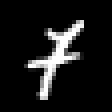
\includegraphics[width=0.2\textwidth]{figures/weakness_rec/MNIST-failure-7(1).png}}
  \caption{Example failure (i.e., misclassification) which classified this image as a $1$ instead of a $7$.}
  \label{fig:mnist_nn_failure}
\end{wrapfigure}
To test our framework, we trained an MNIST classifier to be our black-box system under test $\mathcal{S}$.
We are using the Julia machine learning package \texttt{Flux.jl} \citep{innes:2018} for building the neural network model and training.
The black-box classifier $\mathcal{S}$ consists of two dense layers and a $\ReLU$ activation, mapping the input size of $28\times28=784$ to $32$ activations, and then an output layer of size $10$ (for each digit class).
We use the logit cross-entropy loss, which is equivalent to the cross-entropy loss after applying the $\softmax$ function to the predicted output $\mathbf{\hat y}$:
\begin{equation*}
\mathcal{L}_\mathcal{S}(\softmax(\mathbf{\hat y}), \mathbf{y}) = -\frac{1}{m} \sum_{i=1}^m y_i \log(\hat y_i)
\end{equation*}
We trained the system over $20$ epochs, with a mini-batch size of $1024$, and using the Adam optimizer \citep{kingma2017adam} with a learning rate of $\alpha=3e^{-4}$. This classifier achieves around $93.2\%$ accuracy, so there is room to find weaknesses to exploit failures, where we define a failure as a misclassification.
\Cref{fig:mnist_nn_failure} shows an example failure where the system misclassified a particular digit.




\section{Method}
Our proposed framework, illustrated in \cref{fig:framework}, consists of two major components: a dataset autoencoder, and an adversarial failure selector. These components are iteratively called within a \textit{sampled validation loop}. The dataset autoencoder is used to sample $m$ low-dimensional representations of the encoded input samples $\tilde{\mathbf{x}}$. We encode inputs into a lower-dimensional space for two reasons: 1) to reduce the potential high-dimensionality of the inputs $\mathbf{x}$ and 2) to learn features in this low-dimensional space that likely caused failures.
We then split the $m$ low-dimensional samples into a training set $\tilde{\mathcal{D}}_\text{train}$ and test set $\tilde{\mathcal{D}}_\text{test}$.
The training set $\tilde{\mathcal{D}}_\text{train}$ is passed to an adversarial agent that learns characteristics of the low-dimensional feature representation that led to failures.
We use a failure classifier as our adversary, and then predict which inputs led to failures over the test data $\tilde{\mathcal{D}}_\text{test}$, then map the predicted failures from the low-dimensional space back to the original representation, and then run the candidate inputs expected to result in a failure through the system under test.


\begin{figure}[t]
\centering
\resizebox{0.9\textwidth}{!}{%
    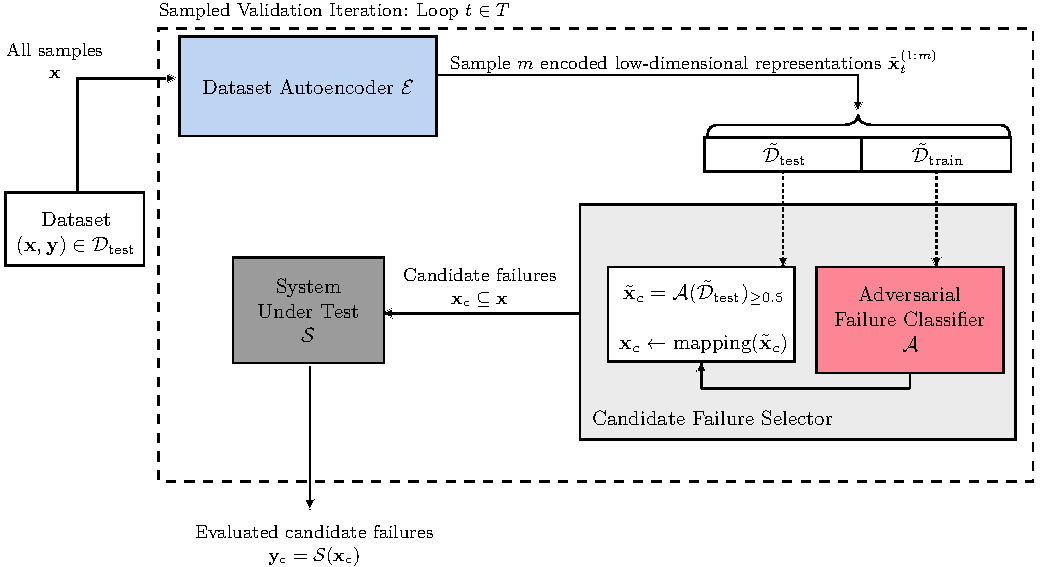
\includegraphics[page=1]{figures/weakness_rec/validation_diagram.pdf}
}
\caption{Validation framework: a dataset autoencoder $\mathcal{E}$ is trained on the entire validation dataset $\mathcal{D}_\text{test}$ consisting of input samples $\mathbf{x}$. Then $m$ samples of encoded low-dimensional representations of the inputs $\tilde{\mathbf{x}}$ are selected for this iteration $t$, denoted $\tilde{\mathbf{x}}_t^{(1:m)}$ for all $m$ samples. The low-dimensional representations are then split into a training and test dataset. The training dataset $\tilde{\mathcal{D}}_\text{train}$ is used to train an adversarial failure classifier $\mathcal{A}$ on the encoded representations. Then the test dataset $\tilde{\mathcal{D}}_\text{test}$ is used to select candidate failures $\tilde{\mathbf{x}}_c$ as predicted by the adversary. Finally, the candidate failures from the adversary $\tilde{\mathbf{x}}_c$ are mapped back to the original inputs $\mathbf{x}_c \subseteq \mathbf{x}$ and evaluated by the system under test $\mathcal{S}$.}
\label{fig:framework}
\end{figure}


\subsection{Dataset Autoencoder}\label{sec:autoencoder}
To get a low-dimensional representation of the inputs $\mathbf{x}$, we used an autoencoder network \citep{kramer1991nonlinear}.
We trained the autoencoder $\mathcal{E}$ on the MNIST test dataset $\mathcal{D}_\text{test}$ and sample from the low-dimensional representation $\tilde{\mathbf{x}}$ as inputs into our adversarial failure classifier.
We use the MNIST test set because this is our input validation set---thus, we want our autoencoder to only have information about the validation set, without the need to have access to the training set used by the system under test.
The autoencoder network maps the $28\times28$ input image $\mathbf x$ into a low-dimensional latent space of size $64$ using a $\LeakyReLU$ activation.
Then the decoder will take the $64$-dimensional representation $\tilde{\mathbf{x}}$, again using a $\LeakyReLU$ activation layer, and attempt to recover the original input $\mathbf x'$.
We pre-trained the autoencoder over $20$ epochs, with a mini-batch size of $1000$, and tuned the network parameters using the Adam optimizer with a learning rate of $\alpha=1e^{-3}$.
Training is unsupervised and we use the mean squared error loss function:
\begin{equation*}
\mathcal{L}_\mathcal{E}(\mathbf{x}', \mathbf{x}) = \frac{1}{m} \sum_{i=1}^m \left( x'_i - x_i \right)^2
\end{equation*}
\Cref{fig:autoencoder_nn} illustrates the autoencoder network architecture and \Cref{fig:mnist_autoencoder} shows samples of the true inputs and their output after encoding/decoding.


\begin{figure*}[!t]
  \centering
    \subfloat[Dataset autoencoder architecture, with inputs $\mathbf{x} \in \mathbb{R}^{28\times28}$, encoded through a dense $\LeakyReLU$ layer of size $\frac{28\times28}{2}$ to a low-dimensional representation $\tilde{\mathbf{x}} \in \mathbb{R}^{64}$, then decoded through a $\LeakyReLU$ layer of size $\frac{28\times28}{2}$, outputting $\mathbf{x}' \in \mathbb{R}^{28\times28}$.]{%
      \resizebox{0.47\textwidth}{!}{
        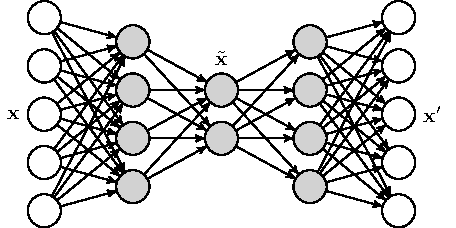
\includegraphics[page=1]{figures/weakness_rec/autoencoder-nn.pdf}
      }
      \label{fig:autoencoder_nn}
    }
    \hspace{2mm}
    \subfloat[Sampled output from the MNIST autoencoder: true input is on top and the recovered input on bottom.]{%
      \resizebox{0.47\textwidth}{!}{
        \centerline{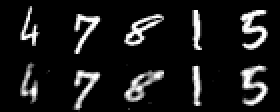
\includegraphics[width=0.6\textwidth]{figures/weakness_rec/sample-MNIST-autoencoder-5.png}}
      }
      \label{fig:mnist_autoencoder}
    }
  \caption{Dataset autoencoder architecture and sample decoded output.} 
\end{figure*}


\subsection{Adversarial Failure Classifier}
To learn the low-dimensional features that are likely to cause failures, we train an adversary $\mathcal{A}$ in the validation loop to classify failures.
The supervised adversary is trained on the partition $\tilde{\mathcal{D}}_\text{train}$ of the low-dimensional samples $\tilde{\mathbf{x}}$ and outputs a prediction that a given input would lead to a system failure.
We train the adversary on the low-dimensional representation for computational efficiency, rather than using the potentially high-dimensional input.
To get the target labels $\mathbf{y}$, we run the system $\mathcal{S}$ using the \textit{true} inputs associated to the \textit{encoded} inputs which are part of the training data $\tilde{\mathcal{D}}_\text{train}$. This gives us targets we can now train our adversary on using the binary cross-entropy loss:
\[
\mathcal L_\mathcal{A}(\mathbf{\hat y}, \mathbf{y}) = -\frac{1}{m}\sum_{i=1}^m y_i\log(\hat y_i) - (1 - y_i)\log(1 - \hat y_i)
\]
The adversarial network architecture consists of $3$ dense layers which map the low-dimensional representation of $\tilde{\mathbf{x}} \in \mathbb{R}^{64}$ through a $\ReLU$ layer of size $128$, another $\ReLU$ layer of size $64$, and finally an output sigmoid layer to map the predictions to a probability.
For each sampled validation iteration $t$ (shown in \Cref{fig:framework}), we retrain the adversary $\mathcal{A}$ for $20$ epochs using the Adam optimizer with learning rate $\alpha=3e^{-5}$. Notice that our learning rate is very small, this is so we do not overfit to early iterations in $t$ and can generalize across different samples of the low-dimensional space. The adversary will use the test data partition $\tilde{\mathcal{D}}_\text{test}$ to select the encoded input that it predicted would lead to a failure.
We use the threshold of $\mathcal{A}(\tilde{x}) \ge 0.5$ to indicate the input $\tilde{x} \in \tilde{\mathcal{D}}_\text{test} \subset (\tilde{\mathbf{x}}, \mathbf{y})$ led to a failure.
All encoded inputs in the test dataset that led to a failure are considered candidate failure scenarios, and we denote them as $\tilde{\mathbf{x}}_c$.
We use a mapping from the encoded inputs $\tilde{\mathbf{x}}_c$ to the original inputs $\mathbf{x}_c \subseteq \mathbf{x}$, and finally pass the failure candidates to the true system $\mathcal{S}$ for evaluation.


\section{Experiments and Results}\label{sec:weakness_experiments}
\begin{table}[b]
    \small
    \centering
    \caption{Evaluation Metrics}\label{tab:metrics}
    \begin{threeparttable}
    \begin{tabular}{@{}lrr|rr@{}}
         \toprule
         \textbf{Failure Selector} &  \textbf{Precision}\tnote{*} & \textbf{Recall}\tnote{*} & \textbf{Sampled Precision}\tnote{$\dagger$} & \textbf{Sampled Recall}\tnote{$\dagger$}\\
         \midrule
         Adversary $\mathcal{A}$ & $0.2441$ & $0.2260$ & $0.2374 \pm 0.11$ & $0.3244 \pm 0.17$ \\
         Random & $0.0647$ & $0.4712$ & $0.0618 \pm 0.04$ & $0.0910 \pm 0.07$ \\
         \bottomrule
    \end{tabular}
    \begin{tablenotes}
        \item[*] {Run over $\mathcal{D}_\text{test}$ only calculated for the ``failure'' class.}
        \item[$\dagger$] {Calculated from $T=10$ iterations of the \textit{sampled validation loop}.}
        \end{tablenotes}
    \end{threeparttable}
\end{table}
To evaluate our approach, we ran $T=10$ sampled validation iterations, sampling $m=500$ random encodings and partitioning these samples in half into $\tilde{\mathcal{D}}_\text{train}$ and $\tilde{\mathcal{D}}_\text{test}$ for the adversary.
Because the failure rate for our system under test is about $0.0677$, we augment the training dataset by duplicating known failures $10$ times after running each training set through the system to get the true outputs $\mathbf{y}_\text{train}$.
We use \textit{precision} and \textit{recall} to evaluate the performance of the adversary. During each iteration $t$, we save off the current adversary $\mathcal{A}_t$ and evaluate the \textit{area under the ROC curve} (AUC) as shown in \Cref{fig:roc}. The ROC curve highlights incremental improvement of the adversary after each iteration. Note that we retrain the new adversary $\mathcal{A}_{t}$ starting from the network weights learning by the previous adversary $\mathcal{A}_{t-1}$.
To balance these metrics, we swept over the prediction threshold to determine which threshold to use (see \Cref{fig:sweep}).
From the tuning sweep, we chose a threshold of $\hat y \ge 0.5$ to indicate a positive failure prediction by the adversary.

During each iteration $t$, the adversary selects $k$ candidate inputs predicted to be likely failures.
For comparison, we employ a random selection of $k$ candidates and evaluate the precision and recall metrics of the random scheme.
This allows us to compare our adversarial learning approach to a baseline and test that our approach is better than guessing randomly. \Cref{tab:metrics} quantifies the evaluation metrics for the adversary and random candidate selector.



\begin{figure*}[t]
    \centering
    \subfloat[ROC curve and AUC for each adversary $\mathcal{A}_t$.]{%
        \resizebox{0.54\textwidth}{!}{%% Creator: Matplotlib, PGF backend
%%
%% To include the figure in your LaTeX document, write
%%   \input{<filename>.pgf}
%%
%% Make sure the required packages are loaded in your preamble
%%   \usepackage{pgf}
%%
%% and, on pdftex
%%   \usepackage[utf8]{inputenc}\DeclareUnicodeCharacter{2212}{-}
%%
%% or, on luatex and xetex
%%   \usepackage{unicode-math}
%%
%% Figures using additional raster images can only be included by \input if
%% they are in the same directory as the main LaTeX file. For loading figures
%% from other directories you can use the `import` package
%%   \usepackage{import}
%%
%% and then include the figures with
%%   \import{<path to file>}{<filename>.pgf}
%%
%% Matplotlib used the following preamble
%%   \usepackage{fontspec}
%%
\begingroup%
\makeatletter%
\begin{pgfpicture}%
\pgfpathrectangle{\pgfpointorigin}{\pgfqpoint{5.729392in}{3.119305in}}%
\pgfusepath{use as bounding box, clip}%
\begin{pgfscope}%
\pgfsetbuttcap%
\pgfsetmiterjoin%
\definecolor{currentfill}{rgb}{1.000000,1.000000,1.000000}%
\pgfsetfillcolor{currentfill}%
\pgfsetlinewidth{0.000000pt}%
\definecolor{currentstroke}{rgb}{1.000000,1.000000,1.000000}%
\pgfsetstrokecolor{currentstroke}%
\pgfsetdash{}{0pt}%
\pgfpathmoveto{\pgfqpoint{0.000000in}{0.000000in}}%
\pgfpathlineto{\pgfqpoint{5.729392in}{0.000000in}}%
\pgfpathlineto{\pgfqpoint{5.729392in}{3.119305in}}%
\pgfpathlineto{\pgfqpoint{0.000000in}{3.119305in}}%
\pgfpathclose%
\pgfusepath{fill}%
\end{pgfscope}%
\begin{pgfscope}%
\pgfsetbuttcap%
\pgfsetmiterjoin%
\definecolor{currentfill}{rgb}{1.000000,1.000000,1.000000}%
\pgfsetfillcolor{currentfill}%
\pgfsetlinewidth{0.000000pt}%
\definecolor{currentstroke}{rgb}{0.000000,0.000000,0.000000}%
\pgfsetstrokecolor{currentstroke}%
\pgfsetstrokeopacity{0.000000}%
\pgfsetdash{}{0pt}%
\pgfpathmoveto{\pgfqpoint{0.896641in}{0.500972in}}%
\pgfpathlineto{\pgfqpoint{3.996641in}{0.500972in}}%
\pgfpathlineto{\pgfqpoint{3.996641in}{2.810972in}}%
\pgfpathlineto{\pgfqpoint{0.896641in}{2.810972in}}%
\pgfpathclose%
\pgfusepath{fill}%
\end{pgfscope}%
\begin{pgfscope}%
\pgfsetbuttcap%
\pgfsetroundjoin%
\definecolor{currentfill}{rgb}{0.000000,0.000000,0.000000}%
\pgfsetfillcolor{currentfill}%
\pgfsetlinewidth{0.803000pt}%
\definecolor{currentstroke}{rgb}{0.000000,0.000000,0.000000}%
\pgfsetstrokecolor{currentstroke}%
\pgfsetdash{}{0pt}%
\pgfsys@defobject{currentmarker}{\pgfqpoint{0.000000in}{-0.048611in}}{\pgfqpoint{0.000000in}{0.000000in}}{%
\pgfpathmoveto{\pgfqpoint{0.000000in}{0.000000in}}%
\pgfpathlineto{\pgfqpoint{0.000000in}{-0.048611in}}%
\pgfusepath{stroke,fill}%
}%
\begin{pgfscope}%
\pgfsys@transformshift{1.037550in}{0.500972in}%
\pgfsys@useobject{currentmarker}{}%
\end{pgfscope}%
\end{pgfscope}%
\begin{pgfscope}%
\definecolor{textcolor}{rgb}{0.000000,0.000000,0.000000}%
\pgfsetstrokecolor{textcolor}%
\pgfsetfillcolor{textcolor}%
\pgftext[x=1.037550in,y=0.403750in,,top]{\color{textcolor}\rmfamily\fontsize{10.000000}{12.000000}\selectfont \(\displaystyle {0.0}\)}%
\end{pgfscope}%
\begin{pgfscope}%
\pgfsetbuttcap%
\pgfsetroundjoin%
\definecolor{currentfill}{rgb}{0.000000,0.000000,0.000000}%
\pgfsetfillcolor{currentfill}%
\pgfsetlinewidth{0.803000pt}%
\definecolor{currentstroke}{rgb}{0.000000,0.000000,0.000000}%
\pgfsetstrokecolor{currentstroke}%
\pgfsetdash{}{0pt}%
\pgfsys@defobject{currentmarker}{\pgfqpoint{0.000000in}{-0.048611in}}{\pgfqpoint{0.000000in}{0.000000in}}{%
\pgfpathmoveto{\pgfqpoint{0.000000in}{0.000000in}}%
\pgfpathlineto{\pgfqpoint{0.000000in}{-0.048611in}}%
\pgfusepath{stroke,fill}%
}%
\begin{pgfscope}%
\pgfsys@transformshift{1.601186in}{0.500972in}%
\pgfsys@useobject{currentmarker}{}%
\end{pgfscope}%
\end{pgfscope}%
\begin{pgfscope}%
\definecolor{textcolor}{rgb}{0.000000,0.000000,0.000000}%
\pgfsetstrokecolor{textcolor}%
\pgfsetfillcolor{textcolor}%
\pgftext[x=1.601186in,y=0.403750in,,top]{\color{textcolor}\rmfamily\fontsize{10.000000}{12.000000}\selectfont \(\displaystyle {0.2}\)}%
\end{pgfscope}%
\begin{pgfscope}%
\pgfsetbuttcap%
\pgfsetroundjoin%
\definecolor{currentfill}{rgb}{0.000000,0.000000,0.000000}%
\pgfsetfillcolor{currentfill}%
\pgfsetlinewidth{0.803000pt}%
\definecolor{currentstroke}{rgb}{0.000000,0.000000,0.000000}%
\pgfsetstrokecolor{currentstroke}%
\pgfsetdash{}{0pt}%
\pgfsys@defobject{currentmarker}{\pgfqpoint{0.000000in}{-0.048611in}}{\pgfqpoint{0.000000in}{0.000000in}}{%
\pgfpathmoveto{\pgfqpoint{0.000000in}{0.000000in}}%
\pgfpathlineto{\pgfqpoint{0.000000in}{-0.048611in}}%
\pgfusepath{stroke,fill}%
}%
\begin{pgfscope}%
\pgfsys@transformshift{2.164823in}{0.500972in}%
\pgfsys@useobject{currentmarker}{}%
\end{pgfscope}%
\end{pgfscope}%
\begin{pgfscope}%
\definecolor{textcolor}{rgb}{0.000000,0.000000,0.000000}%
\pgfsetstrokecolor{textcolor}%
\pgfsetfillcolor{textcolor}%
\pgftext[x=2.164823in,y=0.403750in,,top]{\color{textcolor}\rmfamily\fontsize{10.000000}{12.000000}\selectfont \(\displaystyle {0.4}\)}%
\end{pgfscope}%
\begin{pgfscope}%
\pgfsetbuttcap%
\pgfsetroundjoin%
\definecolor{currentfill}{rgb}{0.000000,0.000000,0.000000}%
\pgfsetfillcolor{currentfill}%
\pgfsetlinewidth{0.803000pt}%
\definecolor{currentstroke}{rgb}{0.000000,0.000000,0.000000}%
\pgfsetstrokecolor{currentstroke}%
\pgfsetdash{}{0pt}%
\pgfsys@defobject{currentmarker}{\pgfqpoint{0.000000in}{-0.048611in}}{\pgfqpoint{0.000000in}{0.000000in}}{%
\pgfpathmoveto{\pgfqpoint{0.000000in}{0.000000in}}%
\pgfpathlineto{\pgfqpoint{0.000000in}{-0.048611in}}%
\pgfusepath{stroke,fill}%
}%
\begin{pgfscope}%
\pgfsys@transformshift{2.728459in}{0.500972in}%
\pgfsys@useobject{currentmarker}{}%
\end{pgfscope}%
\end{pgfscope}%
\begin{pgfscope}%
\definecolor{textcolor}{rgb}{0.000000,0.000000,0.000000}%
\pgfsetstrokecolor{textcolor}%
\pgfsetfillcolor{textcolor}%
\pgftext[x=2.728459in,y=0.403750in,,top]{\color{textcolor}\rmfamily\fontsize{10.000000}{12.000000}\selectfont \(\displaystyle {0.6}\)}%
\end{pgfscope}%
\begin{pgfscope}%
\pgfsetbuttcap%
\pgfsetroundjoin%
\definecolor{currentfill}{rgb}{0.000000,0.000000,0.000000}%
\pgfsetfillcolor{currentfill}%
\pgfsetlinewidth{0.803000pt}%
\definecolor{currentstroke}{rgb}{0.000000,0.000000,0.000000}%
\pgfsetstrokecolor{currentstroke}%
\pgfsetdash{}{0pt}%
\pgfsys@defobject{currentmarker}{\pgfqpoint{0.000000in}{-0.048611in}}{\pgfqpoint{0.000000in}{0.000000in}}{%
\pgfpathmoveto{\pgfqpoint{0.000000in}{0.000000in}}%
\pgfpathlineto{\pgfqpoint{0.000000in}{-0.048611in}}%
\pgfusepath{stroke,fill}%
}%
\begin{pgfscope}%
\pgfsys@transformshift{3.292095in}{0.500972in}%
\pgfsys@useobject{currentmarker}{}%
\end{pgfscope}%
\end{pgfscope}%
\begin{pgfscope}%
\definecolor{textcolor}{rgb}{0.000000,0.000000,0.000000}%
\pgfsetstrokecolor{textcolor}%
\pgfsetfillcolor{textcolor}%
\pgftext[x=3.292095in,y=0.403750in,,top]{\color{textcolor}\rmfamily\fontsize{10.000000}{12.000000}\selectfont \(\displaystyle {0.8}\)}%
\end{pgfscope}%
\begin{pgfscope}%
\pgfsetbuttcap%
\pgfsetroundjoin%
\definecolor{currentfill}{rgb}{0.000000,0.000000,0.000000}%
\pgfsetfillcolor{currentfill}%
\pgfsetlinewidth{0.803000pt}%
\definecolor{currentstroke}{rgb}{0.000000,0.000000,0.000000}%
\pgfsetstrokecolor{currentstroke}%
\pgfsetdash{}{0pt}%
\pgfsys@defobject{currentmarker}{\pgfqpoint{0.000000in}{-0.048611in}}{\pgfqpoint{0.000000in}{0.000000in}}{%
\pgfpathmoveto{\pgfqpoint{0.000000in}{0.000000in}}%
\pgfpathlineto{\pgfqpoint{0.000000in}{-0.048611in}}%
\pgfusepath{stroke,fill}%
}%
\begin{pgfscope}%
\pgfsys@transformshift{3.855732in}{0.500972in}%
\pgfsys@useobject{currentmarker}{}%
\end{pgfscope}%
\end{pgfscope}%
\begin{pgfscope}%
\definecolor{textcolor}{rgb}{0.000000,0.000000,0.000000}%
\pgfsetstrokecolor{textcolor}%
\pgfsetfillcolor{textcolor}%
\pgftext[x=3.855732in,y=0.403750in,,top]{\color{textcolor}\rmfamily\fontsize{10.000000}{12.000000}\selectfont \(\displaystyle {1.0}\)}%
\end{pgfscope}%
\begin{pgfscope}%
\definecolor{textcolor}{rgb}{0.000000,0.000000,0.000000}%
\pgfsetstrokecolor{textcolor}%
\pgfsetfillcolor{textcolor}%
\pgftext[x=2.446641in,y=0.224861in,,top]{\color{textcolor}\rmfamily\fontsize{10.000000}{12.000000}\selectfont false positive rate}%
\end{pgfscope}%
\begin{pgfscope}%
\pgfsetbuttcap%
\pgfsetroundjoin%
\definecolor{currentfill}{rgb}{0.000000,0.000000,0.000000}%
\pgfsetfillcolor{currentfill}%
\pgfsetlinewidth{0.803000pt}%
\definecolor{currentstroke}{rgb}{0.000000,0.000000,0.000000}%
\pgfsetstrokecolor{currentstroke}%
\pgfsetdash{}{0pt}%
\pgfsys@defobject{currentmarker}{\pgfqpoint{-0.048611in}{0.000000in}}{\pgfqpoint{0.000000in}{0.000000in}}{%
\pgfpathmoveto{\pgfqpoint{0.000000in}{0.000000in}}%
\pgfpathlineto{\pgfqpoint{-0.048611in}{0.000000in}}%
\pgfusepath{stroke,fill}%
}%
\begin{pgfscope}%
\pgfsys@transformshift{0.896641in}{0.605972in}%
\pgfsys@useobject{currentmarker}{}%
\end{pgfscope}%
\end{pgfscope}%
\begin{pgfscope}%
\definecolor{textcolor}{rgb}{0.000000,0.000000,0.000000}%
\pgfsetstrokecolor{textcolor}%
\pgfsetfillcolor{textcolor}%
\pgftext[x=0.621949in, y=0.557777in, left, base]{\color{textcolor}\rmfamily\fontsize{10.000000}{12.000000}\selectfont \(\displaystyle {0.0}\)}%
\end{pgfscope}%
\begin{pgfscope}%
\pgfsetbuttcap%
\pgfsetroundjoin%
\definecolor{currentfill}{rgb}{0.000000,0.000000,0.000000}%
\pgfsetfillcolor{currentfill}%
\pgfsetlinewidth{0.803000pt}%
\definecolor{currentstroke}{rgb}{0.000000,0.000000,0.000000}%
\pgfsetstrokecolor{currentstroke}%
\pgfsetdash{}{0pt}%
\pgfsys@defobject{currentmarker}{\pgfqpoint{-0.048611in}{0.000000in}}{\pgfqpoint{0.000000in}{0.000000in}}{%
\pgfpathmoveto{\pgfqpoint{0.000000in}{0.000000in}}%
\pgfpathlineto{\pgfqpoint{-0.048611in}{0.000000in}}%
\pgfusepath{stroke,fill}%
}%
\begin{pgfscope}%
\pgfsys@transformshift{0.896641in}{1.025972in}%
\pgfsys@useobject{currentmarker}{}%
\end{pgfscope}%
\end{pgfscope}%
\begin{pgfscope}%
\definecolor{textcolor}{rgb}{0.000000,0.000000,0.000000}%
\pgfsetstrokecolor{textcolor}%
\pgfsetfillcolor{textcolor}%
\pgftext[x=0.621949in, y=0.977777in, left, base]{\color{textcolor}\rmfamily\fontsize{10.000000}{12.000000}\selectfont \(\displaystyle {0.2}\)}%
\end{pgfscope}%
\begin{pgfscope}%
\pgfsetbuttcap%
\pgfsetroundjoin%
\definecolor{currentfill}{rgb}{0.000000,0.000000,0.000000}%
\pgfsetfillcolor{currentfill}%
\pgfsetlinewidth{0.803000pt}%
\definecolor{currentstroke}{rgb}{0.000000,0.000000,0.000000}%
\pgfsetstrokecolor{currentstroke}%
\pgfsetdash{}{0pt}%
\pgfsys@defobject{currentmarker}{\pgfqpoint{-0.048611in}{0.000000in}}{\pgfqpoint{0.000000in}{0.000000in}}{%
\pgfpathmoveto{\pgfqpoint{0.000000in}{0.000000in}}%
\pgfpathlineto{\pgfqpoint{-0.048611in}{0.000000in}}%
\pgfusepath{stroke,fill}%
}%
\begin{pgfscope}%
\pgfsys@transformshift{0.896641in}{1.445972in}%
\pgfsys@useobject{currentmarker}{}%
\end{pgfscope}%
\end{pgfscope}%
\begin{pgfscope}%
\definecolor{textcolor}{rgb}{0.000000,0.000000,0.000000}%
\pgfsetstrokecolor{textcolor}%
\pgfsetfillcolor{textcolor}%
\pgftext[x=0.621949in, y=1.397777in, left, base]{\color{textcolor}\rmfamily\fontsize{10.000000}{12.000000}\selectfont \(\displaystyle {0.4}\)}%
\end{pgfscope}%
\begin{pgfscope}%
\pgfsetbuttcap%
\pgfsetroundjoin%
\definecolor{currentfill}{rgb}{0.000000,0.000000,0.000000}%
\pgfsetfillcolor{currentfill}%
\pgfsetlinewidth{0.803000pt}%
\definecolor{currentstroke}{rgb}{0.000000,0.000000,0.000000}%
\pgfsetstrokecolor{currentstroke}%
\pgfsetdash{}{0pt}%
\pgfsys@defobject{currentmarker}{\pgfqpoint{-0.048611in}{0.000000in}}{\pgfqpoint{0.000000in}{0.000000in}}{%
\pgfpathmoveto{\pgfqpoint{0.000000in}{0.000000in}}%
\pgfpathlineto{\pgfqpoint{-0.048611in}{0.000000in}}%
\pgfusepath{stroke,fill}%
}%
\begin{pgfscope}%
\pgfsys@transformshift{0.896641in}{1.865972in}%
\pgfsys@useobject{currentmarker}{}%
\end{pgfscope}%
\end{pgfscope}%
\begin{pgfscope}%
\definecolor{textcolor}{rgb}{0.000000,0.000000,0.000000}%
\pgfsetstrokecolor{textcolor}%
\pgfsetfillcolor{textcolor}%
\pgftext[x=0.621949in, y=1.817778in, left, base]{\color{textcolor}\rmfamily\fontsize{10.000000}{12.000000}\selectfont \(\displaystyle {0.6}\)}%
\end{pgfscope}%
\begin{pgfscope}%
\pgfsetbuttcap%
\pgfsetroundjoin%
\definecolor{currentfill}{rgb}{0.000000,0.000000,0.000000}%
\pgfsetfillcolor{currentfill}%
\pgfsetlinewidth{0.803000pt}%
\definecolor{currentstroke}{rgb}{0.000000,0.000000,0.000000}%
\pgfsetstrokecolor{currentstroke}%
\pgfsetdash{}{0pt}%
\pgfsys@defobject{currentmarker}{\pgfqpoint{-0.048611in}{0.000000in}}{\pgfqpoint{0.000000in}{0.000000in}}{%
\pgfpathmoveto{\pgfqpoint{0.000000in}{0.000000in}}%
\pgfpathlineto{\pgfqpoint{-0.048611in}{0.000000in}}%
\pgfusepath{stroke,fill}%
}%
\begin{pgfscope}%
\pgfsys@transformshift{0.896641in}{2.285972in}%
\pgfsys@useobject{currentmarker}{}%
\end{pgfscope}%
\end{pgfscope}%
\begin{pgfscope}%
\definecolor{textcolor}{rgb}{0.000000,0.000000,0.000000}%
\pgfsetstrokecolor{textcolor}%
\pgfsetfillcolor{textcolor}%
\pgftext[x=0.621949in, y=2.237777in, left, base]{\color{textcolor}\rmfamily\fontsize{10.000000}{12.000000}\selectfont \(\displaystyle {0.8}\)}%
\end{pgfscope}%
\begin{pgfscope}%
\pgfsetbuttcap%
\pgfsetroundjoin%
\definecolor{currentfill}{rgb}{0.000000,0.000000,0.000000}%
\pgfsetfillcolor{currentfill}%
\pgfsetlinewidth{0.803000pt}%
\definecolor{currentstroke}{rgb}{0.000000,0.000000,0.000000}%
\pgfsetstrokecolor{currentstroke}%
\pgfsetdash{}{0pt}%
\pgfsys@defobject{currentmarker}{\pgfqpoint{-0.048611in}{0.000000in}}{\pgfqpoint{0.000000in}{0.000000in}}{%
\pgfpathmoveto{\pgfqpoint{0.000000in}{0.000000in}}%
\pgfpathlineto{\pgfqpoint{-0.048611in}{0.000000in}}%
\pgfusepath{stroke,fill}%
}%
\begin{pgfscope}%
\pgfsys@transformshift{0.896641in}{2.705972in}%
\pgfsys@useobject{currentmarker}{}%
\end{pgfscope}%
\end{pgfscope}%
\begin{pgfscope}%
\definecolor{textcolor}{rgb}{0.000000,0.000000,0.000000}%
\pgfsetstrokecolor{textcolor}%
\pgfsetfillcolor{textcolor}%
\pgftext[x=0.621949in, y=2.657778in, left, base]{\color{textcolor}\rmfamily\fontsize{10.000000}{12.000000}\selectfont \(\displaystyle {1.0}\)}%
\end{pgfscope}%
\begin{pgfscope}%
\definecolor{textcolor}{rgb}{0.000000,0.000000,0.000000}%
\pgfsetstrokecolor{textcolor}%
\pgfsetfillcolor{textcolor}%
\pgftext[x=0.566393in,y=1.655972in,,bottom,rotate=90.000000]{\color{textcolor}\rmfamily\fontsize{10.000000}{12.000000}\selectfont true positive rate}%
\end{pgfscope}%
\begin{pgfscope}%
\pgfpathrectangle{\pgfqpoint{0.896641in}{0.500972in}}{\pgfqpoint{3.100000in}{2.310000in}}%
\pgfusepath{clip}%
\pgfsetrectcap%
\pgfsetroundjoin%
\pgfsetlinewidth{1.505625pt}%
\definecolor{currentstroke}{rgb}{0.969000,0.984000,1.000000}%
\pgfsetstrokecolor{currentstroke}%
\pgfsetdash{}{0pt}%
\pgfpathmoveto{\pgfqpoint{1.037550in}{0.605972in}}%
\pgfpathlineto{\pgfqpoint{1.038457in}{0.624583in}}%
\pgfpathlineto{\pgfqpoint{1.040270in}{0.624583in}}%
\pgfpathlineto{\pgfqpoint{1.040270in}{0.627685in}}%
\pgfpathlineto{\pgfqpoint{1.043898in}{0.627685in}}%
\pgfpathlineto{\pgfqpoint{1.044200in}{0.633889in}}%
\pgfpathlineto{\pgfqpoint{1.045107in}{0.633889in}}%
\pgfpathlineto{\pgfqpoint{1.045107in}{0.640093in}}%
\pgfpathlineto{\pgfqpoint{1.046921in}{0.640093in}}%
\pgfpathlineto{\pgfqpoint{1.046921in}{0.643195in}}%
\pgfpathlineto{\pgfqpoint{1.049944in}{0.643195in}}%
\pgfpathlineto{\pgfqpoint{1.050548in}{0.649399in}}%
\pgfpathlineto{\pgfqpoint{1.051153in}{0.649399in}}%
\pgfpathlineto{\pgfqpoint{1.051757in}{0.658705in}}%
\pgfpathlineto{\pgfqpoint{1.053571in}{0.658705in}}%
\pgfpathlineto{\pgfqpoint{1.053873in}{0.668010in}}%
\pgfpathlineto{\pgfqpoint{1.055082in}{0.668010in}}%
\pgfpathlineto{\pgfqpoint{1.055989in}{0.674214in}}%
\pgfpathlineto{\pgfqpoint{1.056896in}{0.674214in}}%
\pgfpathlineto{\pgfqpoint{1.056896in}{0.680418in}}%
\pgfpathlineto{\pgfqpoint{1.059919in}{0.680418in}}%
\pgfpathlineto{\pgfqpoint{1.060826in}{0.686622in}}%
\pgfpathlineto{\pgfqpoint{1.062035in}{0.686622in}}%
\pgfpathlineto{\pgfqpoint{1.062035in}{0.689724in}}%
\pgfpathlineto{\pgfqpoint{1.063546in}{0.689724in}}%
\pgfpathlineto{\pgfqpoint{1.064453in}{0.695928in}}%
\pgfpathlineto{\pgfqpoint{1.066267in}{0.695928in}}%
\pgfpathlineto{\pgfqpoint{1.066267in}{0.702131in}}%
\pgfpathlineto{\pgfqpoint{1.068080in}{0.702131in}}%
\pgfpathlineto{\pgfqpoint{1.068685in}{0.708335in}}%
\pgfpathlineto{\pgfqpoint{1.069592in}{0.708335in}}%
\pgfpathlineto{\pgfqpoint{1.070499in}{0.720743in}}%
\pgfpathlineto{\pgfqpoint{1.071708in}{0.720743in}}%
\pgfpathlineto{\pgfqpoint{1.071708in}{0.723845in}}%
\pgfpathlineto{\pgfqpoint{1.074126in}{0.723845in}}%
\pgfpathlineto{\pgfqpoint{1.075033in}{0.730049in}}%
\pgfpathlineto{\pgfqpoint{1.077451in}{0.730049in}}%
\pgfpathlineto{\pgfqpoint{1.078358in}{0.739355in}}%
\pgfpathlineto{\pgfqpoint{1.080172in}{0.739355in}}%
\pgfpathlineto{\pgfqpoint{1.081079in}{0.754864in}}%
\pgfpathlineto{\pgfqpoint{1.082892in}{0.754864in}}%
\pgfpathlineto{\pgfqpoint{1.083195in}{0.761068in}}%
\pgfpathlineto{\pgfqpoint{1.084706in}{0.761068in}}%
\pgfpathlineto{\pgfqpoint{1.084706in}{0.764170in}}%
\pgfpathlineto{\pgfqpoint{1.089240in}{0.764170in}}%
\pgfpathlineto{\pgfqpoint{1.089240in}{0.767272in}}%
\pgfpathlineto{\pgfqpoint{1.091356in}{0.767272in}}%
\pgfpathlineto{\pgfqpoint{1.091356in}{0.776578in}}%
\pgfpathlineto{\pgfqpoint{1.095588in}{0.776578in}}%
\pgfpathlineto{\pgfqpoint{1.096193in}{0.782781in}}%
\pgfpathlineto{\pgfqpoint{1.099820in}{0.782781in}}%
\pgfpathlineto{\pgfqpoint{1.099820in}{0.788985in}}%
\pgfpathlineto{\pgfqpoint{1.101029in}{0.788985in}}%
\pgfpathlineto{\pgfqpoint{1.101634in}{0.798291in}}%
\pgfpathlineto{\pgfqpoint{1.102843in}{0.798291in}}%
\pgfpathlineto{\pgfqpoint{1.102843in}{0.801393in}}%
\pgfpathlineto{\pgfqpoint{1.105261in}{0.801393in}}%
\pgfpathlineto{\pgfqpoint{1.106168in}{0.813801in}}%
\pgfpathlineto{\pgfqpoint{1.110098in}{0.813801in}}%
\pgfpathlineto{\pgfqpoint{1.110098in}{0.816903in}}%
\pgfpathlineto{\pgfqpoint{1.118259in}{0.816903in}}%
\pgfpathlineto{\pgfqpoint{1.118864in}{0.823106in}}%
\pgfpathlineto{\pgfqpoint{1.122491in}{0.823106in}}%
\pgfpathlineto{\pgfqpoint{1.123398in}{0.832412in}}%
\pgfpathlineto{\pgfqpoint{1.124305in}{0.832412in}}%
\pgfpathlineto{\pgfqpoint{1.124305in}{0.835514in}}%
\pgfpathlineto{\pgfqpoint{1.129142in}{0.835514in}}%
\pgfpathlineto{\pgfqpoint{1.129746in}{0.841718in}}%
\pgfpathlineto{\pgfqpoint{1.132769in}{0.841718in}}%
\pgfpathlineto{\pgfqpoint{1.132769in}{0.844820in}}%
\pgfpathlineto{\pgfqpoint{1.134583in}{0.844820in}}%
\pgfpathlineto{\pgfqpoint{1.134583in}{0.847922in}}%
\pgfpathlineto{\pgfqpoint{1.137001in}{0.847922in}}%
\pgfpathlineto{\pgfqpoint{1.137001in}{0.851024in}}%
\pgfpathlineto{\pgfqpoint{1.139721in}{0.851024in}}%
\pgfpathlineto{\pgfqpoint{1.139721in}{0.854126in}}%
\pgfpathlineto{\pgfqpoint{1.142140in}{0.854126in}}%
\pgfpathlineto{\pgfqpoint{1.143047in}{0.860329in}}%
\pgfpathlineto{\pgfqpoint{1.150301in}{0.860329in}}%
\pgfpathlineto{\pgfqpoint{1.150301in}{0.863431in}}%
\pgfpathlineto{\pgfqpoint{1.153022in}{0.863431in}}%
\pgfpathlineto{\pgfqpoint{1.153022in}{0.869635in}}%
\pgfpathlineto{\pgfqpoint{1.157254in}{0.869635in}}%
\pgfpathlineto{\pgfqpoint{1.158161in}{0.878941in}}%
\pgfpathlineto{\pgfqpoint{1.162695in}{0.878941in}}%
\pgfpathlineto{\pgfqpoint{1.162695in}{0.882043in}}%
\pgfpathlineto{\pgfqpoint{1.166020in}{0.882043in}}%
\pgfpathlineto{\pgfqpoint{1.166927in}{0.888247in}}%
\pgfpathlineto{\pgfqpoint{1.179623in}{0.888247in}}%
\pgfpathlineto{\pgfqpoint{1.180530in}{0.900654in}}%
\pgfpathlineto{\pgfqpoint{1.183250in}{0.900654in}}%
\pgfpathlineto{\pgfqpoint{1.183250in}{0.903756in}}%
\pgfpathlineto{\pgfqpoint{1.184762in}{0.903756in}}%
\pgfpathlineto{\pgfqpoint{1.185064in}{0.909960in}}%
\pgfpathlineto{\pgfqpoint{1.188691in}{0.909960in}}%
\pgfpathlineto{\pgfqpoint{1.188691in}{0.919266in}}%
\pgfpathlineto{\pgfqpoint{1.191714in}{0.919266in}}%
\pgfpathlineto{\pgfqpoint{1.192016in}{0.928572in}}%
\pgfpathlineto{\pgfqpoint{1.192923in}{0.928572in}}%
\pgfpathlineto{\pgfqpoint{1.192923in}{0.931674in}}%
\pgfpathlineto{\pgfqpoint{1.198062in}{0.931674in}}%
\pgfpathlineto{\pgfqpoint{1.198969in}{0.940979in}}%
\pgfpathlineto{\pgfqpoint{1.199876in}{0.940979in}}%
\pgfpathlineto{\pgfqpoint{1.199876in}{0.944081in}}%
\pgfpathlineto{\pgfqpoint{1.201085in}{0.944081in}}%
\pgfpathlineto{\pgfqpoint{1.201387in}{0.950285in}}%
\pgfpathlineto{\pgfqpoint{1.202596in}{0.950285in}}%
\pgfpathlineto{\pgfqpoint{1.202596in}{0.953387in}}%
\pgfpathlineto{\pgfqpoint{1.206526in}{0.953387in}}%
\pgfpathlineto{\pgfqpoint{1.206526in}{0.956489in}}%
\pgfpathlineto{\pgfqpoint{1.211665in}{0.956489in}}%
\pgfpathlineto{\pgfqpoint{1.211665in}{0.959591in}}%
\pgfpathlineto{\pgfqpoint{1.216501in}{0.959591in}}%
\pgfpathlineto{\pgfqpoint{1.216501in}{0.962693in}}%
\pgfpathlineto{\pgfqpoint{1.225872in}{0.962693in}}%
\pgfpathlineto{\pgfqpoint{1.226174in}{0.968897in}}%
\pgfpathlineto{\pgfqpoint{1.228593in}{0.968897in}}%
\pgfpathlineto{\pgfqpoint{1.228593in}{0.971999in}}%
\pgfpathlineto{\pgfqpoint{1.230406in}{0.971999in}}%
\pgfpathlineto{\pgfqpoint{1.230406in}{0.975100in}}%
\pgfpathlineto{\pgfqpoint{1.232825in}{0.975100in}}%
\pgfpathlineto{\pgfqpoint{1.233127in}{0.981304in}}%
\pgfpathlineto{\pgfqpoint{1.234034in}{0.981304in}}%
\pgfpathlineto{\pgfqpoint{1.234336in}{0.987508in}}%
\pgfpathlineto{\pgfqpoint{1.235545in}{0.987508in}}%
\pgfpathlineto{\pgfqpoint{1.235847in}{0.993712in}}%
\pgfpathlineto{\pgfqpoint{1.241591in}{0.993712in}}%
\pgfpathlineto{\pgfqpoint{1.241591in}{0.996814in}}%
\pgfpathlineto{\pgfqpoint{1.243707in}{0.996814in}}%
\pgfpathlineto{\pgfqpoint{1.244009in}{1.003018in}}%
\pgfpathlineto{\pgfqpoint{1.245520in}{1.003018in}}%
\pgfpathlineto{\pgfqpoint{1.245823in}{1.009222in}}%
\pgfpathlineto{\pgfqpoint{1.247636in}{1.009222in}}%
\pgfpathlineto{\pgfqpoint{1.247636in}{1.015425in}}%
\pgfpathlineto{\pgfqpoint{1.252775in}{1.015425in}}%
\pgfpathlineto{\pgfqpoint{1.253078in}{1.021629in}}%
\pgfpathlineto{\pgfqpoint{1.256705in}{1.021629in}}%
\pgfpathlineto{\pgfqpoint{1.257007in}{1.027833in}}%
\pgfpathlineto{\pgfqpoint{1.258216in}{1.027833in}}%
\pgfpathlineto{\pgfqpoint{1.258216in}{1.030935in}}%
\pgfpathlineto{\pgfqpoint{1.262751in}{1.030935in}}%
\pgfpathlineto{\pgfqpoint{1.262751in}{1.034037in}}%
\pgfpathlineto{\pgfqpoint{1.267285in}{1.034037in}}%
\pgfpathlineto{\pgfqpoint{1.267285in}{1.037139in}}%
\pgfpathlineto{\pgfqpoint{1.270912in}{1.037139in}}%
\pgfpathlineto{\pgfqpoint{1.270912in}{1.040241in}}%
\pgfpathlineto{\pgfqpoint{1.273330in}{1.040241in}}%
\pgfpathlineto{\pgfqpoint{1.273330in}{1.043343in}}%
\pgfpathlineto{\pgfqpoint{1.284213in}{1.043343in}}%
\pgfpathlineto{\pgfqpoint{1.284213in}{1.046445in}}%
\pgfpathlineto{\pgfqpoint{1.286026in}{1.046445in}}%
\pgfpathlineto{\pgfqpoint{1.286026in}{1.049547in}}%
\pgfpathlineto{\pgfqpoint{1.288142in}{1.049547in}}%
\pgfpathlineto{\pgfqpoint{1.288142in}{1.052648in}}%
\pgfpathlineto{\pgfqpoint{1.289956in}{1.052648in}}%
\pgfpathlineto{\pgfqpoint{1.289956in}{1.055750in}}%
\pgfpathlineto{\pgfqpoint{1.292072in}{1.055750in}}%
\pgfpathlineto{\pgfqpoint{1.292072in}{1.061954in}}%
\pgfpathlineto{\pgfqpoint{1.299024in}{1.061954in}}%
\pgfpathlineto{\pgfqpoint{1.299024in}{1.065056in}}%
\pgfpathlineto{\pgfqpoint{1.305977in}{1.065056in}}%
\pgfpathlineto{\pgfqpoint{1.306279in}{1.071260in}}%
\pgfpathlineto{\pgfqpoint{1.309000in}{1.071260in}}%
\pgfpathlineto{\pgfqpoint{1.309000in}{1.074362in}}%
\pgfpathlineto{\pgfqpoint{1.313836in}{1.074362in}}%
\pgfpathlineto{\pgfqpoint{1.313836in}{1.077464in}}%
\pgfpathlineto{\pgfqpoint{1.315045in}{1.077464in}}%
\pgfpathlineto{\pgfqpoint{1.315045in}{1.080566in}}%
\pgfpathlineto{\pgfqpoint{1.317161in}{1.080566in}}%
\pgfpathlineto{\pgfqpoint{1.317464in}{1.086770in}}%
\pgfpathlineto{\pgfqpoint{1.322603in}{1.086770in}}%
\pgfpathlineto{\pgfqpoint{1.323509in}{1.092973in}}%
\pgfpathlineto{\pgfqpoint{1.340135in}{1.092973in}}%
\pgfpathlineto{\pgfqpoint{1.340135in}{1.096075in}}%
\pgfpathlineto{\pgfqpoint{1.347692in}{1.096075in}}%
\pgfpathlineto{\pgfqpoint{1.348297in}{1.102279in}}%
\pgfpathlineto{\pgfqpoint{1.348901in}{1.102279in}}%
\pgfpathlineto{\pgfqpoint{1.348901in}{1.105381in}}%
\pgfpathlineto{\pgfqpoint{1.351924in}{1.105381in}}%
\pgfpathlineto{\pgfqpoint{1.351924in}{1.108483in}}%
\pgfpathlineto{\pgfqpoint{1.355551in}{1.108483in}}%
\pgfpathlineto{\pgfqpoint{1.355551in}{1.111585in}}%
\pgfpathlineto{\pgfqpoint{1.360388in}{1.111585in}}%
\pgfpathlineto{\pgfqpoint{1.360388in}{1.114687in}}%
\pgfpathlineto{\pgfqpoint{1.365224in}{1.114687in}}%
\pgfpathlineto{\pgfqpoint{1.366131in}{1.120891in}}%
\pgfpathlineto{\pgfqpoint{1.367038in}{1.120891in}}%
\pgfpathlineto{\pgfqpoint{1.367340in}{1.127095in}}%
\pgfpathlineto{\pgfqpoint{1.371572in}{1.127095in}}%
\pgfpathlineto{\pgfqpoint{1.371572in}{1.130196in}}%
\pgfpathlineto{\pgfqpoint{1.374293in}{1.130196in}}%
\pgfpathlineto{\pgfqpoint{1.374293in}{1.136400in}}%
\pgfpathlineto{\pgfqpoint{1.376409in}{1.136400in}}%
\pgfpathlineto{\pgfqpoint{1.377013in}{1.142604in}}%
\pgfpathlineto{\pgfqpoint{1.378525in}{1.142604in}}%
\pgfpathlineto{\pgfqpoint{1.378525in}{1.145706in}}%
\pgfpathlineto{\pgfqpoint{1.380036in}{1.145706in}}%
\pgfpathlineto{\pgfqpoint{1.380036in}{1.148808in}}%
\pgfpathlineto{\pgfqpoint{1.386082in}{1.148808in}}%
\pgfpathlineto{\pgfqpoint{1.386082in}{1.151910in}}%
\pgfpathlineto{\pgfqpoint{1.388500in}{1.151910in}}%
\pgfpathlineto{\pgfqpoint{1.388500in}{1.155012in}}%
\pgfpathlineto{\pgfqpoint{1.400894in}{1.155012in}}%
\pgfpathlineto{\pgfqpoint{1.400894in}{1.158114in}}%
\pgfpathlineto{\pgfqpoint{1.408451in}{1.158114in}}%
\pgfpathlineto{\pgfqpoint{1.409358in}{1.164318in}}%
\pgfpathlineto{\pgfqpoint{1.410567in}{1.164318in}}%
\pgfpathlineto{\pgfqpoint{1.411171in}{1.170521in}}%
\pgfpathlineto{\pgfqpoint{1.416915in}{1.170521in}}%
\pgfpathlineto{\pgfqpoint{1.416915in}{1.176725in}}%
\pgfpathlineto{\pgfqpoint{1.419635in}{1.176725in}}%
\pgfpathlineto{\pgfqpoint{1.419635in}{1.179827in}}%
\pgfpathlineto{\pgfqpoint{1.426588in}{1.179827in}}%
\pgfpathlineto{\pgfqpoint{1.426890in}{1.189133in}}%
\pgfpathlineto{\pgfqpoint{1.430517in}{1.189133in}}%
\pgfpathlineto{\pgfqpoint{1.430517in}{1.192235in}}%
\pgfpathlineto{\pgfqpoint{1.433238in}{1.192235in}}%
\pgfpathlineto{\pgfqpoint{1.433540in}{1.198439in}}%
\pgfpathlineto{\pgfqpoint{1.440191in}{1.198439in}}%
\pgfpathlineto{\pgfqpoint{1.440191in}{1.201541in}}%
\pgfpathlineto{\pgfqpoint{1.444422in}{1.201541in}}%
\pgfpathlineto{\pgfqpoint{1.444422in}{1.204643in}}%
\pgfpathlineto{\pgfqpoint{1.448050in}{1.204643in}}%
\pgfpathlineto{\pgfqpoint{1.448050in}{1.210846in}}%
\pgfpathlineto{\pgfqpoint{1.454700in}{1.210846in}}%
\pgfpathlineto{\pgfqpoint{1.454700in}{1.213948in}}%
\pgfpathlineto{\pgfqpoint{1.459537in}{1.213948in}}%
\pgfpathlineto{\pgfqpoint{1.459537in}{1.217050in}}%
\pgfpathlineto{\pgfqpoint{1.465885in}{1.217050in}}%
\pgfpathlineto{\pgfqpoint{1.465885in}{1.220152in}}%
\pgfpathlineto{\pgfqpoint{1.467698in}{1.220152in}}%
\pgfpathlineto{\pgfqpoint{1.467698in}{1.223254in}}%
\pgfpathlineto{\pgfqpoint{1.469814in}{1.223254in}}%
\pgfpathlineto{\pgfqpoint{1.470116in}{1.229458in}}%
\pgfpathlineto{\pgfqpoint{1.471326in}{1.229458in}}%
\pgfpathlineto{\pgfqpoint{1.471930in}{1.235662in}}%
\pgfpathlineto{\pgfqpoint{1.488556in}{1.235662in}}%
\pgfpathlineto{\pgfqpoint{1.488556in}{1.238764in}}%
\pgfpathlineto{\pgfqpoint{1.490067in}{1.238764in}}%
\pgfpathlineto{\pgfqpoint{1.490067in}{1.241866in}}%
\pgfpathlineto{\pgfqpoint{1.493392in}{1.241866in}}%
\pgfpathlineto{\pgfqpoint{1.493695in}{1.248069in}}%
\pgfpathlineto{\pgfqpoint{1.495811in}{1.248069in}}%
\pgfpathlineto{\pgfqpoint{1.495811in}{1.251171in}}%
\pgfpathlineto{\pgfqpoint{1.500345in}{1.251171in}}%
\pgfpathlineto{\pgfqpoint{1.500345in}{1.254273in}}%
\pgfpathlineto{\pgfqpoint{1.501554in}{1.254273in}}%
\pgfpathlineto{\pgfqpoint{1.501554in}{1.257375in}}%
\pgfpathlineto{\pgfqpoint{1.503972in}{1.257375in}}%
\pgfpathlineto{\pgfqpoint{1.504879in}{1.263579in}}%
\pgfpathlineto{\pgfqpoint{1.514552in}{1.263579in}}%
\pgfpathlineto{\pgfqpoint{1.514552in}{1.266681in}}%
\pgfpathlineto{\pgfqpoint{1.535410in}{1.266681in}}%
\pgfpathlineto{\pgfqpoint{1.535410in}{1.269783in}}%
\pgfpathlineto{\pgfqpoint{1.539944in}{1.269783in}}%
\pgfpathlineto{\pgfqpoint{1.539944in}{1.272885in}}%
\pgfpathlineto{\pgfqpoint{1.542664in}{1.272885in}}%
\pgfpathlineto{\pgfqpoint{1.542664in}{1.275987in}}%
\pgfpathlineto{\pgfqpoint{1.544780in}{1.275987in}}%
\pgfpathlineto{\pgfqpoint{1.544780in}{1.279089in}}%
\pgfpathlineto{\pgfqpoint{1.546594in}{1.279089in}}%
\pgfpathlineto{\pgfqpoint{1.547199in}{1.285292in}}%
\pgfpathlineto{\pgfqpoint{1.555058in}{1.285292in}}%
\pgfpathlineto{\pgfqpoint{1.555058in}{1.288394in}}%
\pgfpathlineto{\pgfqpoint{1.558988in}{1.288394in}}%
\pgfpathlineto{\pgfqpoint{1.558988in}{1.291496in}}%
\pgfpathlineto{\pgfqpoint{1.568661in}{1.291496in}}%
\pgfpathlineto{\pgfqpoint{1.568661in}{1.294598in}}%
\pgfpathlineto{\pgfqpoint{1.572893in}{1.294598in}}%
\pgfpathlineto{\pgfqpoint{1.572893in}{1.297700in}}%
\pgfpathlineto{\pgfqpoint{1.574404in}{1.297700in}}%
\pgfpathlineto{\pgfqpoint{1.574404in}{1.300802in}}%
\pgfpathlineto{\pgfqpoint{1.582868in}{1.300802in}}%
\pgfpathlineto{\pgfqpoint{1.582868in}{1.303904in}}%
\pgfpathlineto{\pgfqpoint{1.585588in}{1.303904in}}%
\pgfpathlineto{\pgfqpoint{1.585588in}{1.310108in}}%
\pgfpathlineto{\pgfqpoint{1.590425in}{1.310108in}}%
\pgfpathlineto{\pgfqpoint{1.590425in}{1.313210in}}%
\pgfpathlineto{\pgfqpoint{1.594052in}{1.313210in}}%
\pgfpathlineto{\pgfqpoint{1.594052in}{1.316312in}}%
\pgfpathlineto{\pgfqpoint{1.601005in}{1.316312in}}%
\pgfpathlineto{\pgfqpoint{1.601005in}{1.319414in}}%
\pgfpathlineto{\pgfqpoint{1.603725in}{1.319414in}}%
\pgfpathlineto{\pgfqpoint{1.603725in}{1.322516in}}%
\pgfpathlineto{\pgfqpoint{1.607051in}{1.322516in}}%
\pgfpathlineto{\pgfqpoint{1.607051in}{1.325617in}}%
\pgfpathlineto{\pgfqpoint{1.617328in}{1.325617in}}%
\pgfpathlineto{\pgfqpoint{1.617933in}{1.331821in}}%
\pgfpathlineto{\pgfqpoint{1.619746in}{1.331821in}}%
\pgfpathlineto{\pgfqpoint{1.619746in}{1.338025in}}%
\pgfpathlineto{\pgfqpoint{1.620956in}{1.338025in}}%
\pgfpathlineto{\pgfqpoint{1.620956in}{1.341127in}}%
\pgfpathlineto{\pgfqpoint{1.627304in}{1.341127in}}%
\pgfpathlineto{\pgfqpoint{1.627304in}{1.344229in}}%
\pgfpathlineto{\pgfqpoint{1.639999in}{1.344229in}}%
\pgfpathlineto{\pgfqpoint{1.639999in}{1.347331in}}%
\pgfpathlineto{\pgfqpoint{1.641511in}{1.347331in}}%
\pgfpathlineto{\pgfqpoint{1.641511in}{1.353535in}}%
\pgfpathlineto{\pgfqpoint{1.644534in}{1.353535in}}%
\pgfpathlineto{\pgfqpoint{1.644534in}{1.359739in}}%
\pgfpathlineto{\pgfqpoint{1.651486in}{1.359739in}}%
\pgfpathlineto{\pgfqpoint{1.651486in}{1.362840in}}%
\pgfpathlineto{\pgfqpoint{1.652998in}{1.362840in}}%
\pgfpathlineto{\pgfqpoint{1.653904in}{1.372146in}}%
\pgfpathlineto{\pgfqpoint{1.655718in}{1.372146in}}%
\pgfpathlineto{\pgfqpoint{1.656323in}{1.378350in}}%
\pgfpathlineto{\pgfqpoint{1.658741in}{1.378350in}}%
\pgfpathlineto{\pgfqpoint{1.658741in}{1.381452in}}%
\pgfpathlineto{\pgfqpoint{1.661764in}{1.381452in}}%
\pgfpathlineto{\pgfqpoint{1.661764in}{1.384554in}}%
\pgfpathlineto{\pgfqpoint{1.663880in}{1.384554in}}%
\pgfpathlineto{\pgfqpoint{1.663880in}{1.387656in}}%
\pgfpathlineto{\pgfqpoint{1.667205in}{1.387656in}}%
\pgfpathlineto{\pgfqpoint{1.667205in}{1.390758in}}%
\pgfpathlineto{\pgfqpoint{1.679296in}{1.390758in}}%
\pgfpathlineto{\pgfqpoint{1.679296in}{1.393860in}}%
\pgfpathlineto{\pgfqpoint{1.688365in}{1.393860in}}%
\pgfpathlineto{\pgfqpoint{1.688365in}{1.400064in}}%
\pgfpathlineto{\pgfqpoint{1.694713in}{1.400064in}}%
\pgfpathlineto{\pgfqpoint{1.694713in}{1.403165in}}%
\pgfpathlineto{\pgfqpoint{1.697433in}{1.403165in}}%
\pgfpathlineto{\pgfqpoint{1.697433in}{1.406267in}}%
\pgfpathlineto{\pgfqpoint{1.700456in}{1.406267in}}%
\pgfpathlineto{\pgfqpoint{1.700456in}{1.409369in}}%
\pgfpathlineto{\pgfqpoint{1.701967in}{1.409369in}}%
\pgfpathlineto{\pgfqpoint{1.701967in}{1.412471in}}%
\pgfpathlineto{\pgfqpoint{1.703781in}{1.412471in}}%
\pgfpathlineto{\pgfqpoint{1.704688in}{1.418675in}}%
\pgfpathlineto{\pgfqpoint{1.705292in}{1.418675in}}%
\pgfpathlineto{\pgfqpoint{1.705292in}{1.421777in}}%
\pgfpathlineto{\pgfqpoint{1.708920in}{1.421777in}}%
\pgfpathlineto{\pgfqpoint{1.708920in}{1.424879in}}%
\pgfpathlineto{\pgfqpoint{1.711036in}{1.424879in}}%
\pgfpathlineto{\pgfqpoint{1.711036in}{1.431083in}}%
\pgfpathlineto{\pgfqpoint{1.716175in}{1.431083in}}%
\pgfpathlineto{\pgfqpoint{1.716175in}{1.434185in}}%
\pgfpathlineto{\pgfqpoint{1.725848in}{1.434185in}}%
\pgfpathlineto{\pgfqpoint{1.725848in}{1.437287in}}%
\pgfpathlineto{\pgfqpoint{1.733707in}{1.437287in}}%
\pgfpathlineto{\pgfqpoint{1.733707in}{1.440388in}}%
\pgfpathlineto{\pgfqpoint{1.737637in}{1.440388in}}%
\pgfpathlineto{\pgfqpoint{1.737637in}{1.443490in}}%
\pgfpathlineto{\pgfqpoint{1.739450in}{1.443490in}}%
\pgfpathlineto{\pgfqpoint{1.739450in}{1.446592in}}%
\pgfpathlineto{\pgfqpoint{1.743380in}{1.446592in}}%
\pgfpathlineto{\pgfqpoint{1.743380in}{1.449694in}}%
\pgfpathlineto{\pgfqpoint{1.748519in}{1.449694in}}%
\pgfpathlineto{\pgfqpoint{1.748519in}{1.452796in}}%
\pgfpathlineto{\pgfqpoint{1.750937in}{1.452796in}}%
\pgfpathlineto{\pgfqpoint{1.750937in}{1.455898in}}%
\pgfpathlineto{\pgfqpoint{1.752751in}{1.455898in}}%
\pgfpathlineto{\pgfqpoint{1.752751in}{1.459000in}}%
\pgfpathlineto{\pgfqpoint{1.754867in}{1.459000in}}%
\pgfpathlineto{\pgfqpoint{1.754867in}{1.462102in}}%
\pgfpathlineto{\pgfqpoint{1.761517in}{1.462102in}}%
\pgfpathlineto{\pgfqpoint{1.761517in}{1.468306in}}%
\pgfpathlineto{\pgfqpoint{1.762726in}{1.468306in}}%
\pgfpathlineto{\pgfqpoint{1.762726in}{1.471408in}}%
\pgfpathlineto{\pgfqpoint{1.764842in}{1.471408in}}%
\pgfpathlineto{\pgfqpoint{1.764842in}{1.474510in}}%
\pgfpathlineto{\pgfqpoint{1.766051in}{1.474510in}}%
\pgfpathlineto{\pgfqpoint{1.766051in}{1.477612in}}%
\pgfpathlineto{\pgfqpoint{1.769679in}{1.477612in}}%
\pgfpathlineto{\pgfqpoint{1.769679in}{1.480713in}}%
\pgfpathlineto{\pgfqpoint{1.776933in}{1.480713in}}%
\pgfpathlineto{\pgfqpoint{1.776933in}{1.483815in}}%
\pgfpathlineto{\pgfqpoint{1.784793in}{1.483815in}}%
\pgfpathlineto{\pgfqpoint{1.784793in}{1.486917in}}%
\pgfpathlineto{\pgfqpoint{1.789932in}{1.486917in}}%
\pgfpathlineto{\pgfqpoint{1.789932in}{1.490019in}}%
\pgfpathlineto{\pgfqpoint{1.792350in}{1.490019in}}%
\pgfpathlineto{\pgfqpoint{1.792350in}{1.493121in}}%
\pgfpathlineto{\pgfqpoint{1.794164in}{1.493121in}}%
\pgfpathlineto{\pgfqpoint{1.794466in}{1.499325in}}%
\pgfpathlineto{\pgfqpoint{1.805046in}{1.499325in}}%
\pgfpathlineto{\pgfqpoint{1.805046in}{1.502427in}}%
\pgfpathlineto{\pgfqpoint{1.807766in}{1.502427in}}%
\pgfpathlineto{\pgfqpoint{1.807766in}{1.505529in}}%
\pgfpathlineto{\pgfqpoint{1.813207in}{1.505529in}}%
\pgfpathlineto{\pgfqpoint{1.813207in}{1.508631in}}%
\pgfpathlineto{\pgfqpoint{1.819253in}{1.508631in}}%
\pgfpathlineto{\pgfqpoint{1.819253in}{1.511733in}}%
\pgfpathlineto{\pgfqpoint{1.821067in}{1.511733in}}%
\pgfpathlineto{\pgfqpoint{1.821067in}{1.514835in}}%
\pgfpathlineto{\pgfqpoint{1.828322in}{1.514835in}}%
\pgfpathlineto{\pgfqpoint{1.828322in}{1.517936in}}%
\pgfpathlineto{\pgfqpoint{1.831344in}{1.517936in}}%
\pgfpathlineto{\pgfqpoint{1.831344in}{1.521038in}}%
\pgfpathlineto{\pgfqpoint{1.834065in}{1.521038in}}%
\pgfpathlineto{\pgfqpoint{1.834065in}{1.524140in}}%
\pgfpathlineto{\pgfqpoint{1.836483in}{1.524140in}}%
\pgfpathlineto{\pgfqpoint{1.836483in}{1.527242in}}%
\pgfpathlineto{\pgfqpoint{1.847365in}{1.527242in}}%
\pgfpathlineto{\pgfqpoint{1.847365in}{1.530344in}}%
\pgfpathlineto{\pgfqpoint{1.853411in}{1.530344in}}%
\pgfpathlineto{\pgfqpoint{1.853411in}{1.533446in}}%
\pgfpathlineto{\pgfqpoint{1.860968in}{1.533446in}}%
\pgfpathlineto{\pgfqpoint{1.860968in}{1.542752in}}%
\pgfpathlineto{\pgfqpoint{1.863084in}{1.542752in}}%
\pgfpathlineto{\pgfqpoint{1.863084in}{1.545854in}}%
\pgfpathlineto{\pgfqpoint{1.864595in}{1.545854in}}%
\pgfpathlineto{\pgfqpoint{1.864595in}{1.548956in}}%
\pgfpathlineto{\pgfqpoint{1.867316in}{1.548956in}}%
\pgfpathlineto{\pgfqpoint{1.867316in}{1.552058in}}%
\pgfpathlineto{\pgfqpoint{1.881523in}{1.552058in}}%
\pgfpathlineto{\pgfqpoint{1.882128in}{1.558261in}}%
\pgfpathlineto{\pgfqpoint{1.885453in}{1.558261in}}%
\pgfpathlineto{\pgfqpoint{1.885453in}{1.561363in}}%
\pgfpathlineto{\pgfqpoint{1.894521in}{1.561363in}}%
\pgfpathlineto{\pgfqpoint{1.894521in}{1.567567in}}%
\pgfpathlineto{\pgfqpoint{1.899660in}{1.567567in}}%
\pgfpathlineto{\pgfqpoint{1.899660in}{1.570669in}}%
\pgfpathlineto{\pgfqpoint{1.908124in}{1.570669in}}%
\pgfpathlineto{\pgfqpoint{1.908729in}{1.576873in}}%
\pgfpathlineto{\pgfqpoint{1.916890in}{1.576873in}}%
\pgfpathlineto{\pgfqpoint{1.916890in}{1.579975in}}%
\pgfpathlineto{\pgfqpoint{1.923843in}{1.579975in}}%
\pgfpathlineto{\pgfqpoint{1.924447in}{1.586179in}}%
\pgfpathlineto{\pgfqpoint{1.934725in}{1.586179in}}%
\pgfpathlineto{\pgfqpoint{1.934725in}{1.589281in}}%
\pgfpathlineto{\pgfqpoint{1.954978in}{1.589281in}}%
\pgfpathlineto{\pgfqpoint{1.954978in}{1.592383in}}%
\pgfpathlineto{\pgfqpoint{1.960117in}{1.592383in}}%
\pgfpathlineto{\pgfqpoint{1.960117in}{1.595484in}}%
\pgfpathlineto{\pgfqpoint{1.976440in}{1.595484in}}%
\pgfpathlineto{\pgfqpoint{1.977347in}{1.607892in}}%
\pgfpathlineto{\pgfqpoint{1.978254in}{1.607892in}}%
\pgfpathlineto{\pgfqpoint{1.978254in}{1.610994in}}%
\pgfpathlineto{\pgfqpoint{1.986415in}{1.610994in}}%
\pgfpathlineto{\pgfqpoint{1.987020in}{1.620300in}}%
\pgfpathlineto{\pgfqpoint{1.994577in}{1.620300in}}%
\pgfpathlineto{\pgfqpoint{1.994577in}{1.623402in}}%
\pgfpathlineto{\pgfqpoint{1.996088in}{1.623402in}}%
\pgfpathlineto{\pgfqpoint{1.996088in}{1.626504in}}%
\pgfpathlineto{\pgfqpoint{2.000018in}{1.626504in}}%
\pgfpathlineto{\pgfqpoint{2.000623in}{1.632708in}}%
\pgfpathlineto{\pgfqpoint{2.002739in}{1.632708in}}%
\pgfpathlineto{\pgfqpoint{2.002739in}{1.635809in}}%
\pgfpathlineto{\pgfqpoint{2.010900in}{1.635809in}}%
\pgfpathlineto{\pgfqpoint{2.011203in}{1.642013in}}%
\pgfpathlineto{\pgfqpoint{2.012109in}{1.642013in}}%
\pgfpathlineto{\pgfqpoint{2.012109in}{1.645115in}}%
\pgfpathlineto{\pgfqpoint{2.019969in}{1.645115in}}%
\pgfpathlineto{\pgfqpoint{2.019969in}{1.651319in}}%
\pgfpathlineto{\pgfqpoint{2.022992in}{1.651319in}}%
\pgfpathlineto{\pgfqpoint{2.022992in}{1.654421in}}%
\pgfpathlineto{\pgfqpoint{2.026317in}{1.654421in}}%
\pgfpathlineto{\pgfqpoint{2.026317in}{1.657523in}}%
\pgfpathlineto{\pgfqpoint{2.029944in}{1.657523in}}%
\pgfpathlineto{\pgfqpoint{2.029944in}{1.660625in}}%
\pgfpathlineto{\pgfqpoint{2.035990in}{1.660625in}}%
\pgfpathlineto{\pgfqpoint{2.035990in}{1.663727in}}%
\pgfpathlineto{\pgfqpoint{2.041129in}{1.663727in}}%
\pgfpathlineto{\pgfqpoint{2.041733in}{1.673033in}}%
\pgfpathlineto{\pgfqpoint{2.042942in}{1.673033in}}%
\pgfpathlineto{\pgfqpoint{2.043547in}{1.679236in}}%
\pgfpathlineto{\pgfqpoint{2.046872in}{1.679236in}}%
\pgfpathlineto{\pgfqpoint{2.046872in}{1.682338in}}%
\pgfpathlineto{\pgfqpoint{2.048686in}{1.682338in}}%
\pgfpathlineto{\pgfqpoint{2.048686in}{1.685440in}}%
\pgfpathlineto{\pgfqpoint{2.051104in}{1.685440in}}%
\pgfpathlineto{\pgfqpoint{2.051104in}{1.688542in}}%
\pgfpathlineto{\pgfqpoint{2.063195in}{1.688542in}}%
\pgfpathlineto{\pgfqpoint{2.063195in}{1.691644in}}%
\pgfpathlineto{\pgfqpoint{2.069241in}{1.691644in}}%
\pgfpathlineto{\pgfqpoint{2.069241in}{1.694746in}}%
\pgfpathlineto{\pgfqpoint{2.070752in}{1.694746in}}%
\pgfpathlineto{\pgfqpoint{2.070752in}{1.697848in}}%
\pgfpathlineto{\pgfqpoint{2.074077in}{1.697848in}}%
\pgfpathlineto{\pgfqpoint{2.074077in}{1.700950in}}%
\pgfpathlineto{\pgfqpoint{2.078612in}{1.700950in}}%
\pgfpathlineto{\pgfqpoint{2.078612in}{1.704052in}}%
\pgfpathlineto{\pgfqpoint{2.082239in}{1.704052in}}%
\pgfpathlineto{\pgfqpoint{2.082239in}{1.707154in}}%
\pgfpathlineto{\pgfqpoint{2.084657in}{1.707154in}}%
\pgfpathlineto{\pgfqpoint{2.084657in}{1.710256in}}%
\pgfpathlineto{\pgfqpoint{2.087076in}{1.710256in}}%
\pgfpathlineto{\pgfqpoint{2.087076in}{1.716459in}}%
\pgfpathlineto{\pgfqpoint{2.089494in}{1.716459in}}%
\pgfpathlineto{\pgfqpoint{2.089494in}{1.719561in}}%
\pgfpathlineto{\pgfqpoint{2.090703in}{1.719561in}}%
\pgfpathlineto{\pgfqpoint{2.090703in}{1.722663in}}%
\pgfpathlineto{\pgfqpoint{2.093423in}{1.722663in}}%
\pgfpathlineto{\pgfqpoint{2.093726in}{1.728867in}}%
\pgfpathlineto{\pgfqpoint{2.099771in}{1.728867in}}%
\pgfpathlineto{\pgfqpoint{2.100376in}{1.738173in}}%
\pgfpathlineto{\pgfqpoint{2.101887in}{1.738173in}}%
\pgfpathlineto{\pgfqpoint{2.101887in}{1.741275in}}%
\pgfpathlineto{\pgfqpoint{2.107026in}{1.741275in}}%
\pgfpathlineto{\pgfqpoint{2.107026in}{1.744377in}}%
\pgfpathlineto{\pgfqpoint{2.116095in}{1.744377in}}%
\pgfpathlineto{\pgfqpoint{2.116095in}{1.747479in}}%
\pgfpathlineto{\pgfqpoint{2.119420in}{1.747479in}}%
\pgfpathlineto{\pgfqpoint{2.119420in}{1.753682in}}%
\pgfpathlineto{\pgfqpoint{2.122443in}{1.753682in}}%
\pgfpathlineto{\pgfqpoint{2.122443in}{1.756784in}}%
\pgfpathlineto{\pgfqpoint{2.126070in}{1.756784in}}%
\pgfpathlineto{\pgfqpoint{2.126977in}{1.762988in}}%
\pgfpathlineto{\pgfqpoint{2.130604in}{1.762988in}}%
\pgfpathlineto{\pgfqpoint{2.130604in}{1.766090in}}%
\pgfpathlineto{\pgfqpoint{2.134232in}{1.766090in}}%
\pgfpathlineto{\pgfqpoint{2.135138in}{1.772294in}}%
\pgfpathlineto{\pgfqpoint{2.136348in}{1.772294in}}%
\pgfpathlineto{\pgfqpoint{2.136348in}{1.775396in}}%
\pgfpathlineto{\pgfqpoint{2.147230in}{1.775396in}}%
\pgfpathlineto{\pgfqpoint{2.147230in}{1.778498in}}%
\pgfpathlineto{\pgfqpoint{2.151159in}{1.778498in}}%
\pgfpathlineto{\pgfqpoint{2.151159in}{1.781600in}}%
\pgfpathlineto{\pgfqpoint{2.156903in}{1.781600in}}%
\pgfpathlineto{\pgfqpoint{2.156903in}{1.784702in}}%
\pgfpathlineto{\pgfqpoint{2.159926in}{1.784702in}}%
\pgfpathlineto{\pgfqpoint{2.159926in}{1.787804in}}%
\pgfpathlineto{\pgfqpoint{2.161739in}{1.787804in}}%
\pgfpathlineto{\pgfqpoint{2.161739in}{1.790905in}}%
\pgfpathlineto{\pgfqpoint{2.165669in}{1.790905in}}%
\pgfpathlineto{\pgfqpoint{2.165669in}{1.794007in}}%
\pgfpathlineto{\pgfqpoint{2.166878in}{1.794007in}}%
\pgfpathlineto{\pgfqpoint{2.166878in}{1.797109in}}%
\pgfpathlineto{\pgfqpoint{2.168692in}{1.797109in}}%
\pgfpathlineto{\pgfqpoint{2.168692in}{1.800211in}}%
\pgfpathlineto{\pgfqpoint{2.172622in}{1.800211in}}%
\pgfpathlineto{\pgfqpoint{2.172622in}{1.803313in}}%
\pgfpathlineto{\pgfqpoint{2.174738in}{1.803313in}}%
\pgfpathlineto{\pgfqpoint{2.175644in}{1.812619in}}%
\pgfpathlineto{\pgfqpoint{2.178063in}{1.812619in}}%
\pgfpathlineto{\pgfqpoint{2.178063in}{1.815721in}}%
\pgfpathlineto{\pgfqpoint{2.184411in}{1.815721in}}%
\pgfpathlineto{\pgfqpoint{2.184411in}{1.818823in}}%
\pgfpathlineto{\pgfqpoint{2.185620in}{1.818823in}}%
\pgfpathlineto{\pgfqpoint{2.185620in}{1.821925in}}%
\pgfpathlineto{\pgfqpoint{2.198920in}{1.821925in}}%
\pgfpathlineto{\pgfqpoint{2.198920in}{1.825027in}}%
\pgfpathlineto{\pgfqpoint{2.200734in}{1.825027in}}%
\pgfpathlineto{\pgfqpoint{2.201641in}{1.831230in}}%
\pgfpathlineto{\pgfqpoint{2.208895in}{1.831230in}}%
\pgfpathlineto{\pgfqpoint{2.208895in}{1.834332in}}%
\pgfpathlineto{\pgfqpoint{2.211011in}{1.834332in}}%
\pgfpathlineto{\pgfqpoint{2.211011in}{1.837434in}}%
\pgfpathlineto{\pgfqpoint{2.212523in}{1.837434in}}%
\pgfpathlineto{\pgfqpoint{2.212523in}{1.840536in}}%
\pgfpathlineto{\pgfqpoint{2.213732in}{1.840536in}}%
\pgfpathlineto{\pgfqpoint{2.213732in}{1.843638in}}%
\pgfpathlineto{\pgfqpoint{2.220080in}{1.843638in}}%
\pgfpathlineto{\pgfqpoint{2.220080in}{1.846740in}}%
\pgfpathlineto{\pgfqpoint{2.224614in}{1.846740in}}%
\pgfpathlineto{\pgfqpoint{2.224614in}{1.849842in}}%
\pgfpathlineto{\pgfqpoint{2.226126in}{1.849842in}}%
\pgfpathlineto{\pgfqpoint{2.226126in}{1.852944in}}%
\pgfpathlineto{\pgfqpoint{2.234590in}{1.852944in}}%
\pgfpathlineto{\pgfqpoint{2.234590in}{1.856046in}}%
\pgfpathlineto{\pgfqpoint{2.244263in}{1.856046in}}%
\pgfpathlineto{\pgfqpoint{2.244263in}{1.859148in}}%
\pgfpathlineto{\pgfqpoint{2.250913in}{1.859148in}}%
\pgfpathlineto{\pgfqpoint{2.250913in}{1.862250in}}%
\pgfpathlineto{\pgfqpoint{2.264515in}{1.862250in}}%
\pgfpathlineto{\pgfqpoint{2.264515in}{1.865352in}}%
\pgfpathlineto{\pgfqpoint{2.284466in}{1.865352in}}%
\pgfpathlineto{\pgfqpoint{2.284466in}{1.868453in}}%
\pgfpathlineto{\pgfqpoint{2.288698in}{1.868453in}}%
\pgfpathlineto{\pgfqpoint{2.289000in}{1.874657in}}%
\pgfpathlineto{\pgfqpoint{2.295046in}{1.874657in}}%
\pgfpathlineto{\pgfqpoint{2.295046in}{1.877759in}}%
\pgfpathlineto{\pgfqpoint{2.297162in}{1.877759in}}%
\pgfpathlineto{\pgfqpoint{2.297464in}{1.883963in}}%
\pgfpathlineto{\pgfqpoint{2.306231in}{1.883963in}}%
\pgfpathlineto{\pgfqpoint{2.306231in}{1.887065in}}%
\pgfpathlineto{\pgfqpoint{2.311067in}{1.887065in}}%
\pgfpathlineto{\pgfqpoint{2.311067in}{1.890167in}}%
\pgfpathlineto{\pgfqpoint{2.328902in}{1.890167in}}%
\pgfpathlineto{\pgfqpoint{2.329204in}{1.896371in}}%
\pgfpathlineto{\pgfqpoint{2.330715in}{1.896371in}}%
\pgfpathlineto{\pgfqpoint{2.331018in}{1.902575in}}%
\pgfpathlineto{\pgfqpoint{2.334041in}{1.902575in}}%
\pgfpathlineto{\pgfqpoint{2.334041in}{1.905677in}}%
\pgfpathlineto{\pgfqpoint{2.353084in}{1.905677in}}%
\pgfpathlineto{\pgfqpoint{2.353084in}{1.908778in}}%
\pgfpathlineto{\pgfqpoint{2.355200in}{1.908778in}}%
\pgfpathlineto{\pgfqpoint{2.355200in}{1.911880in}}%
\pgfpathlineto{\pgfqpoint{2.367594in}{1.911880in}}%
\pgfpathlineto{\pgfqpoint{2.367594in}{1.914982in}}%
\pgfpathlineto{\pgfqpoint{2.370012in}{1.914982in}}%
\pgfpathlineto{\pgfqpoint{2.370012in}{1.918084in}}%
\pgfpathlineto{\pgfqpoint{2.371826in}{1.918084in}}%
\pgfpathlineto{\pgfqpoint{2.371826in}{1.921186in}}%
\pgfpathlineto{\pgfqpoint{2.375756in}{1.921186in}}%
\pgfpathlineto{\pgfqpoint{2.375756in}{1.927390in}}%
\pgfpathlineto{\pgfqpoint{2.395404in}{1.927390in}}%
\pgfpathlineto{\pgfqpoint{2.395404in}{1.930492in}}%
\pgfpathlineto{\pgfqpoint{2.397822in}{1.930492in}}%
\pgfpathlineto{\pgfqpoint{2.397822in}{1.933594in}}%
\pgfpathlineto{\pgfqpoint{2.399031in}{1.933594in}}%
\pgfpathlineto{\pgfqpoint{2.399031in}{1.936696in}}%
\pgfpathlineto{\pgfqpoint{2.402659in}{1.936696in}}%
\pgfpathlineto{\pgfqpoint{2.402659in}{1.939798in}}%
\pgfpathlineto{\pgfqpoint{2.404170in}{1.939798in}}%
\pgfpathlineto{\pgfqpoint{2.404170in}{1.942900in}}%
\pgfpathlineto{\pgfqpoint{2.408704in}{1.942900in}}%
\pgfpathlineto{\pgfqpoint{2.408704in}{1.946001in}}%
\pgfpathlineto{\pgfqpoint{2.410518in}{1.946001in}}%
\pgfpathlineto{\pgfqpoint{2.410518in}{1.949103in}}%
\pgfpathlineto{\pgfqpoint{2.412332in}{1.949103in}}%
\pgfpathlineto{\pgfqpoint{2.412936in}{1.955307in}}%
\pgfpathlineto{\pgfqpoint{2.416261in}{1.955307in}}%
\pgfpathlineto{\pgfqpoint{2.417168in}{1.961511in}}%
\pgfpathlineto{\pgfqpoint{2.424121in}{1.961511in}}%
\pgfpathlineto{\pgfqpoint{2.424121in}{1.964613in}}%
\pgfpathlineto{\pgfqpoint{2.439537in}{1.964613in}}%
\pgfpathlineto{\pgfqpoint{2.439537in}{1.967715in}}%
\pgfpathlineto{\pgfqpoint{2.450722in}{1.967715in}}%
\pgfpathlineto{\pgfqpoint{2.450722in}{1.970817in}}%
\pgfpathlineto{\pgfqpoint{2.452838in}{1.970817in}}%
\pgfpathlineto{\pgfqpoint{2.452838in}{1.973919in}}%
\pgfpathlineto{\pgfqpoint{2.454047in}{1.973919in}}%
\pgfpathlineto{\pgfqpoint{2.454047in}{1.977021in}}%
\pgfpathlineto{\pgfqpoint{2.460395in}{1.977021in}}%
\pgfpathlineto{\pgfqpoint{2.460395in}{1.980123in}}%
\pgfpathlineto{\pgfqpoint{2.464627in}{1.980123in}}%
\pgfpathlineto{\pgfqpoint{2.464627in}{1.983225in}}%
\pgfpathlineto{\pgfqpoint{2.470672in}{1.983225in}}%
\pgfpathlineto{\pgfqpoint{2.470672in}{1.986326in}}%
\pgfpathlineto{\pgfqpoint{2.471881in}{1.986326in}}%
\pgfpathlineto{\pgfqpoint{2.472486in}{1.992530in}}%
\pgfpathlineto{\pgfqpoint{2.477020in}{1.992530in}}%
\pgfpathlineto{\pgfqpoint{2.477020in}{1.995632in}}%
\pgfpathlineto{\pgfqpoint{2.478229in}{1.995632in}}%
\pgfpathlineto{\pgfqpoint{2.478229in}{1.998734in}}%
\pgfpathlineto{\pgfqpoint{2.481857in}{1.998734in}}%
\pgfpathlineto{\pgfqpoint{2.481857in}{2.001836in}}%
\pgfpathlineto{\pgfqpoint{2.486089in}{2.001836in}}%
\pgfpathlineto{\pgfqpoint{2.486089in}{2.004938in}}%
\pgfpathlineto{\pgfqpoint{2.514201in}{2.004938in}}%
\pgfpathlineto{\pgfqpoint{2.514201in}{2.008040in}}%
\pgfpathlineto{\pgfqpoint{2.518433in}{2.008040in}}%
\pgfpathlineto{\pgfqpoint{2.518433in}{2.011142in}}%
\pgfpathlineto{\pgfqpoint{2.530222in}{2.011142in}}%
\pgfpathlineto{\pgfqpoint{2.530222in}{2.014244in}}%
\pgfpathlineto{\pgfqpoint{2.531733in}{2.014244in}}%
\pgfpathlineto{\pgfqpoint{2.531733in}{2.017346in}}%
\pgfpathlineto{\pgfqpoint{2.534454in}{2.017346in}}%
\pgfpathlineto{\pgfqpoint{2.534454in}{2.020448in}}%
\pgfpathlineto{\pgfqpoint{2.536570in}{2.020448in}}%
\pgfpathlineto{\pgfqpoint{2.536570in}{2.023549in}}%
\pgfpathlineto{\pgfqpoint{2.545638in}{2.023549in}}%
\pgfpathlineto{\pgfqpoint{2.546243in}{2.032855in}}%
\pgfpathlineto{\pgfqpoint{2.549870in}{2.032855in}}%
\pgfpathlineto{\pgfqpoint{2.550475in}{2.042161in}}%
\pgfpathlineto{\pgfqpoint{2.551080in}{2.042161in}}%
\pgfpathlineto{\pgfqpoint{2.551080in}{2.045263in}}%
\pgfpathlineto{\pgfqpoint{2.555614in}{2.045263in}}%
\pgfpathlineto{\pgfqpoint{2.555614in}{2.048365in}}%
\pgfpathlineto{\pgfqpoint{2.561962in}{2.048365in}}%
\pgfpathlineto{\pgfqpoint{2.561962in}{2.051467in}}%
\pgfpathlineto{\pgfqpoint{2.565891in}{2.051467in}}%
\pgfpathlineto{\pgfqpoint{2.565891in}{2.054569in}}%
\pgfpathlineto{\pgfqpoint{2.575564in}{2.054569in}}%
\pgfpathlineto{\pgfqpoint{2.575564in}{2.057671in}}%
\pgfpathlineto{\pgfqpoint{2.591283in}{2.057671in}}%
\pgfpathlineto{\pgfqpoint{2.591283in}{2.060773in}}%
\pgfpathlineto{\pgfqpoint{2.609420in}{2.060773in}}%
\pgfpathlineto{\pgfqpoint{2.609420in}{2.063874in}}%
\pgfpathlineto{\pgfqpoint{2.611234in}{2.063874in}}%
\pgfpathlineto{\pgfqpoint{2.612141in}{2.070078in}}%
\pgfpathlineto{\pgfqpoint{2.614257in}{2.070078in}}%
\pgfpathlineto{\pgfqpoint{2.615163in}{2.076282in}}%
\pgfpathlineto{\pgfqpoint{2.616675in}{2.076282in}}%
\pgfpathlineto{\pgfqpoint{2.616675in}{2.079384in}}%
\pgfpathlineto{\pgfqpoint{2.627255in}{2.079384in}}%
\pgfpathlineto{\pgfqpoint{2.627255in}{2.085588in}}%
\pgfpathlineto{\pgfqpoint{2.633905in}{2.085588in}}%
\pgfpathlineto{\pgfqpoint{2.634510in}{2.091792in}}%
\pgfpathlineto{\pgfqpoint{2.645694in}{2.091792in}}%
\pgfpathlineto{\pgfqpoint{2.645694in}{2.094894in}}%
\pgfpathlineto{\pgfqpoint{2.648717in}{2.094894in}}%
\pgfpathlineto{\pgfqpoint{2.648717in}{2.097996in}}%
\pgfpathlineto{\pgfqpoint{2.658390in}{2.097996in}}%
\pgfpathlineto{\pgfqpoint{2.658390in}{2.101097in}}%
\pgfpathlineto{\pgfqpoint{2.663831in}{2.101097in}}%
\pgfpathlineto{\pgfqpoint{2.664738in}{2.107301in}}%
\pgfpathlineto{\pgfqpoint{2.684991in}{2.107301in}}%
\pgfpathlineto{\pgfqpoint{2.684991in}{2.110403in}}%
\pgfpathlineto{\pgfqpoint{2.687711in}{2.110403in}}%
\pgfpathlineto{\pgfqpoint{2.687711in}{2.113505in}}%
\pgfpathlineto{\pgfqpoint{2.690130in}{2.113505in}}%
\pgfpathlineto{\pgfqpoint{2.690130in}{2.116607in}}%
\pgfpathlineto{\pgfqpoint{2.694059in}{2.116607in}}%
\pgfpathlineto{\pgfqpoint{2.694664in}{2.122811in}}%
\pgfpathlineto{\pgfqpoint{2.714010in}{2.122811in}}%
\pgfpathlineto{\pgfqpoint{2.714010in}{2.125913in}}%
\pgfpathlineto{\pgfqpoint{2.716428in}{2.125913in}}%
\pgfpathlineto{\pgfqpoint{2.717335in}{2.132117in}}%
\pgfpathlineto{\pgfqpoint{2.725497in}{2.132117in}}%
\pgfpathlineto{\pgfqpoint{2.725497in}{2.135219in}}%
\pgfpathlineto{\pgfqpoint{2.731542in}{2.135219in}}%
\pgfpathlineto{\pgfqpoint{2.731542in}{2.138321in}}%
\pgfpathlineto{\pgfqpoint{2.733961in}{2.138321in}}%
\pgfpathlineto{\pgfqpoint{2.733961in}{2.141422in}}%
\pgfpathlineto{\pgfqpoint{2.742424in}{2.141422in}}%
\pgfpathlineto{\pgfqpoint{2.742424in}{2.144524in}}%
\pgfpathlineto{\pgfqpoint{2.746656in}{2.144524in}}%
\pgfpathlineto{\pgfqpoint{2.746656in}{2.147626in}}%
\pgfpathlineto{\pgfqpoint{2.747866in}{2.147626in}}%
\pgfpathlineto{\pgfqpoint{2.747866in}{2.150728in}}%
\pgfpathlineto{\pgfqpoint{2.751191in}{2.150728in}}%
\pgfpathlineto{\pgfqpoint{2.751795in}{2.156932in}}%
\pgfpathlineto{\pgfqpoint{2.755423in}{2.156932in}}%
\pgfpathlineto{\pgfqpoint{2.755423in}{2.160034in}}%
\pgfpathlineto{\pgfqpoint{2.776582in}{2.160034in}}%
\pgfpathlineto{\pgfqpoint{2.776582in}{2.163136in}}%
\pgfpathlineto{\pgfqpoint{2.785953in}{2.163136in}}%
\pgfpathlineto{\pgfqpoint{2.785953in}{2.166238in}}%
\pgfpathlineto{\pgfqpoint{2.787465in}{2.166238in}}%
\pgfpathlineto{\pgfqpoint{2.787465in}{2.169340in}}%
\pgfpathlineto{\pgfqpoint{2.791697in}{2.169340in}}%
\pgfpathlineto{\pgfqpoint{2.791697in}{2.172442in}}%
\pgfpathlineto{\pgfqpoint{2.811647in}{2.172442in}}%
\pgfpathlineto{\pgfqpoint{2.811647in}{2.175544in}}%
\pgfpathlineto{\pgfqpoint{2.821018in}{2.175544in}}%
\pgfpathlineto{\pgfqpoint{2.821018in}{2.178646in}}%
\pgfpathlineto{\pgfqpoint{2.823739in}{2.178646in}}%
\pgfpathlineto{\pgfqpoint{2.823739in}{2.181747in}}%
\pgfpathlineto{\pgfqpoint{2.830691in}{2.181747in}}%
\pgfpathlineto{\pgfqpoint{2.830691in}{2.184849in}}%
\pgfpathlineto{\pgfqpoint{2.835528in}{2.184849in}}%
\pgfpathlineto{\pgfqpoint{2.835528in}{2.187951in}}%
\pgfpathlineto{\pgfqpoint{2.837039in}{2.187951in}}%
\pgfpathlineto{\pgfqpoint{2.837946in}{2.194155in}}%
\pgfpathlineto{\pgfqpoint{2.860617in}{2.194155in}}%
\pgfpathlineto{\pgfqpoint{2.860617in}{2.197257in}}%
\pgfpathlineto{\pgfqpoint{2.865454in}{2.197257in}}%
\pgfpathlineto{\pgfqpoint{2.865454in}{2.200359in}}%
\pgfpathlineto{\pgfqpoint{2.868174in}{2.200359in}}%
\pgfpathlineto{\pgfqpoint{2.868174in}{2.203461in}}%
\pgfpathlineto{\pgfqpoint{2.877243in}{2.203461in}}%
\pgfpathlineto{\pgfqpoint{2.877243in}{2.206563in}}%
\pgfpathlineto{\pgfqpoint{2.882079in}{2.206563in}}%
\pgfpathlineto{\pgfqpoint{2.882079in}{2.209665in}}%
\pgfpathlineto{\pgfqpoint{2.885706in}{2.209665in}}%
\pgfpathlineto{\pgfqpoint{2.885706in}{2.212767in}}%
\pgfpathlineto{\pgfqpoint{2.886916in}{2.212767in}}%
\pgfpathlineto{\pgfqpoint{2.886916in}{2.215869in}}%
\pgfpathlineto{\pgfqpoint{2.896589in}{2.215869in}}%
\pgfpathlineto{\pgfqpoint{2.896589in}{2.218970in}}%
\pgfpathlineto{\pgfqpoint{2.899611in}{2.218970in}}%
\pgfpathlineto{\pgfqpoint{2.899611in}{2.222072in}}%
\pgfpathlineto{\pgfqpoint{2.902030in}{2.222072in}}%
\pgfpathlineto{\pgfqpoint{2.902030in}{2.225174in}}%
\pgfpathlineto{\pgfqpoint{2.921980in}{2.225174in}}%
\pgfpathlineto{\pgfqpoint{2.922585in}{2.231378in}}%
\pgfpathlineto{\pgfqpoint{2.923492in}{2.231378in}}%
\pgfpathlineto{\pgfqpoint{2.923492in}{2.234480in}}%
\pgfpathlineto{\pgfqpoint{2.925003in}{2.234480in}}%
\pgfpathlineto{\pgfqpoint{2.925003in}{2.237582in}}%
\pgfpathlineto{\pgfqpoint{2.928026in}{2.237582in}}%
\pgfpathlineto{\pgfqpoint{2.928026in}{2.240684in}}%
\pgfpathlineto{\pgfqpoint{2.932560in}{2.240684in}}%
\pgfpathlineto{\pgfqpoint{2.932560in}{2.246888in}}%
\pgfpathlineto{\pgfqpoint{2.934072in}{2.246888in}}%
\pgfpathlineto{\pgfqpoint{2.934072in}{2.249990in}}%
\pgfpathlineto{\pgfqpoint{2.937095in}{2.249990in}}%
\pgfpathlineto{\pgfqpoint{2.937095in}{2.253092in}}%
\pgfpathlineto{\pgfqpoint{2.947977in}{2.253092in}}%
\pgfpathlineto{\pgfqpoint{2.947977in}{2.256194in}}%
\pgfpathlineto{\pgfqpoint{2.954929in}{2.256194in}}%
\pgfpathlineto{\pgfqpoint{2.954929in}{2.259295in}}%
\pgfpathlineto{\pgfqpoint{2.976391in}{2.259295in}}%
\pgfpathlineto{\pgfqpoint{2.976391in}{2.262397in}}%
\pgfpathlineto{\pgfqpoint{2.983344in}{2.262397in}}%
\pgfpathlineto{\pgfqpoint{2.983344in}{2.265499in}}%
\pgfpathlineto{\pgfqpoint{2.996644in}{2.265499in}}%
\pgfpathlineto{\pgfqpoint{2.996644in}{2.268601in}}%
\pgfpathlineto{\pgfqpoint{3.006015in}{2.268601in}}%
\pgfpathlineto{\pgfqpoint{3.006922in}{2.274805in}}%
\pgfpathlineto{\pgfqpoint{3.013572in}{2.274805in}}%
\pgfpathlineto{\pgfqpoint{3.013572in}{2.277907in}}%
\pgfpathlineto{\pgfqpoint{3.036243in}{2.277907in}}%
\pgfpathlineto{\pgfqpoint{3.036243in}{2.281009in}}%
\pgfpathlineto{\pgfqpoint{3.039568in}{2.281009in}}%
\pgfpathlineto{\pgfqpoint{3.039568in}{2.284111in}}%
\pgfpathlineto{\pgfqpoint{3.041684in}{2.284111in}}%
\pgfpathlineto{\pgfqpoint{3.041684in}{2.287213in}}%
\pgfpathlineto{\pgfqpoint{3.057705in}{2.287213in}}%
\pgfpathlineto{\pgfqpoint{3.057705in}{2.290315in}}%
\pgfpathlineto{\pgfqpoint{3.061937in}{2.290315in}}%
\pgfpathlineto{\pgfqpoint{3.061937in}{2.293417in}}%
\pgfpathlineto{\pgfqpoint{3.063146in}{2.293417in}}%
\pgfpathlineto{\pgfqpoint{3.063146in}{2.296518in}}%
\pgfpathlineto{\pgfqpoint{3.087934in}{2.296518in}}%
\pgfpathlineto{\pgfqpoint{3.088236in}{2.302722in}}%
\pgfpathlineto{\pgfqpoint{3.098816in}{2.302722in}}%
\pgfpathlineto{\pgfqpoint{3.099723in}{2.308926in}}%
\pgfpathlineto{\pgfqpoint{3.100932in}{2.308926in}}%
\pgfpathlineto{\pgfqpoint{3.100932in}{2.312028in}}%
\pgfpathlineto{\pgfqpoint{3.106675in}{2.312028in}}%
\pgfpathlineto{\pgfqpoint{3.106675in}{2.315130in}}%
\pgfpathlineto{\pgfqpoint{3.108489in}{2.315130in}}%
\pgfpathlineto{\pgfqpoint{3.108489in}{2.318232in}}%
\pgfpathlineto{\pgfqpoint{3.121185in}{2.318232in}}%
\pgfpathlineto{\pgfqpoint{3.122092in}{2.324436in}}%
\pgfpathlineto{\pgfqpoint{3.126021in}{2.324436in}}%
\pgfpathlineto{\pgfqpoint{3.126021in}{2.327538in}}%
\pgfpathlineto{\pgfqpoint{3.129346in}{2.327538in}}%
\pgfpathlineto{\pgfqpoint{3.129951in}{2.333742in}}%
\pgfpathlineto{\pgfqpoint{3.130555in}{2.333742in}}%
\pgfpathlineto{\pgfqpoint{3.130555in}{2.336843in}}%
\pgfpathlineto{\pgfqpoint{3.140833in}{2.336843in}}%
\pgfpathlineto{\pgfqpoint{3.140833in}{2.339945in}}%
\pgfpathlineto{\pgfqpoint{3.142647in}{2.339945in}}%
\pgfpathlineto{\pgfqpoint{3.143251in}{2.346149in}}%
\pgfpathlineto{\pgfqpoint{3.145065in}{2.346149in}}%
\pgfpathlineto{\pgfqpoint{3.145065in}{2.349251in}}%
\pgfpathlineto{\pgfqpoint{3.156552in}{2.349251in}}%
\pgfpathlineto{\pgfqpoint{3.156552in}{2.352353in}}%
\pgfpathlineto{\pgfqpoint{3.169852in}{2.352353in}}%
\pgfpathlineto{\pgfqpoint{3.169852in}{2.355455in}}%
\pgfpathlineto{\pgfqpoint{3.181641in}{2.355455in}}%
\pgfpathlineto{\pgfqpoint{3.181641in}{2.358557in}}%
\pgfpathlineto{\pgfqpoint{3.188594in}{2.358557in}}%
\pgfpathlineto{\pgfqpoint{3.188594in}{2.361659in}}%
\pgfpathlineto{\pgfqpoint{3.191617in}{2.361659in}}%
\pgfpathlineto{\pgfqpoint{3.191617in}{2.364761in}}%
\pgfpathlineto{\pgfqpoint{3.195849in}{2.364761in}}%
\pgfpathlineto{\pgfqpoint{3.195849in}{2.367863in}}%
\pgfpathlineto{\pgfqpoint{3.204615in}{2.367863in}}%
\pgfpathlineto{\pgfqpoint{3.204615in}{2.370965in}}%
\pgfpathlineto{\pgfqpoint{3.213683in}{2.370965in}}%
\pgfpathlineto{\pgfqpoint{3.213683in}{2.374066in}}%
\pgfpathlineto{\pgfqpoint{3.221845in}{2.374066in}}%
\pgfpathlineto{\pgfqpoint{3.221845in}{2.377168in}}%
\pgfpathlineto{\pgfqpoint{3.224565in}{2.377168in}}%
\pgfpathlineto{\pgfqpoint{3.224565in}{2.380270in}}%
\pgfpathlineto{\pgfqpoint{3.232425in}{2.380270in}}%
\pgfpathlineto{\pgfqpoint{3.232425in}{2.383372in}}%
\pgfpathlineto{\pgfqpoint{3.248748in}{2.383372in}}%
\pgfpathlineto{\pgfqpoint{3.248748in}{2.386474in}}%
\pgfpathlineto{\pgfqpoint{3.254794in}{2.386474in}}%
\pgfpathlineto{\pgfqpoint{3.254794in}{2.389576in}}%
\pgfpathlineto{\pgfqpoint{3.258421in}{2.389576in}}%
\pgfpathlineto{\pgfqpoint{3.258421in}{2.392678in}}%
\pgfpathlineto{\pgfqpoint{3.261444in}{2.392678in}}%
\pgfpathlineto{\pgfqpoint{3.261444in}{2.395780in}}%
\pgfpathlineto{\pgfqpoint{3.265374in}{2.395780in}}%
\pgfpathlineto{\pgfqpoint{3.265374in}{2.398882in}}%
\pgfpathlineto{\pgfqpoint{3.266583in}{2.398882in}}%
\pgfpathlineto{\pgfqpoint{3.266583in}{2.401984in}}%
\pgfpathlineto{\pgfqpoint{3.271117in}{2.401984in}}%
\pgfpathlineto{\pgfqpoint{3.271117in}{2.405086in}}%
\pgfpathlineto{\pgfqpoint{3.275953in}{2.405086in}}%
\pgfpathlineto{\pgfqpoint{3.275953in}{2.408188in}}%
\pgfpathlineto{\pgfqpoint{3.279279in}{2.408188in}}%
\pgfpathlineto{\pgfqpoint{3.280185in}{2.414391in}}%
\pgfpathlineto{\pgfqpoint{3.295602in}{2.414391in}}%
\pgfpathlineto{\pgfqpoint{3.295602in}{2.417493in}}%
\pgfpathlineto{\pgfqpoint{3.297718in}{2.417493in}}%
\pgfpathlineto{\pgfqpoint{3.297718in}{2.420595in}}%
\pgfpathlineto{\pgfqpoint{3.302252in}{2.420595in}}%
\pgfpathlineto{\pgfqpoint{3.302252in}{2.423697in}}%
\pgfpathlineto{\pgfqpoint{3.311018in}{2.423697in}}%
\pgfpathlineto{\pgfqpoint{3.311018in}{2.426799in}}%
\pgfpathlineto{\pgfqpoint{3.318273in}{2.426799in}}%
\pgfpathlineto{\pgfqpoint{3.318273in}{2.429901in}}%
\pgfpathlineto{\pgfqpoint{3.323714in}{2.429901in}}%
\pgfpathlineto{\pgfqpoint{3.323714in}{2.433003in}}%
\pgfpathlineto{\pgfqpoint{3.330062in}{2.433003in}}%
\pgfpathlineto{\pgfqpoint{3.330364in}{2.442309in}}%
\pgfpathlineto{\pgfqpoint{3.333387in}{2.442309in}}%
\pgfpathlineto{\pgfqpoint{3.333689in}{2.448513in}}%
\pgfpathlineto{\pgfqpoint{3.340340in}{2.448513in}}%
\pgfpathlineto{\pgfqpoint{3.340340in}{2.451614in}}%
\pgfpathlineto{\pgfqpoint{3.355756in}{2.451614in}}%
\pgfpathlineto{\pgfqpoint{3.355756in}{2.454716in}}%
\pgfpathlineto{\pgfqpoint{3.360593in}{2.454716in}}%
\pgfpathlineto{\pgfqpoint{3.360593in}{2.457818in}}%
\pgfpathlineto{\pgfqpoint{3.369359in}{2.457818in}}%
\pgfpathlineto{\pgfqpoint{3.369359in}{2.460920in}}%
\pgfpathlineto{\pgfqpoint{3.371777in}{2.460920in}}%
\pgfpathlineto{\pgfqpoint{3.371777in}{2.464022in}}%
\pgfpathlineto{\pgfqpoint{3.375404in}{2.464022in}}%
\pgfpathlineto{\pgfqpoint{3.376009in}{2.470226in}}%
\pgfpathlineto{\pgfqpoint{3.383264in}{2.470226in}}%
\pgfpathlineto{\pgfqpoint{3.383264in}{2.473328in}}%
\pgfpathlineto{\pgfqpoint{3.385984in}{2.473328in}}%
\pgfpathlineto{\pgfqpoint{3.385984in}{2.476430in}}%
\pgfpathlineto{\pgfqpoint{3.394751in}{2.476430in}}%
\pgfpathlineto{\pgfqpoint{3.394751in}{2.479532in}}%
\pgfpathlineto{\pgfqpoint{3.398680in}{2.479532in}}%
\pgfpathlineto{\pgfqpoint{3.398680in}{2.482634in}}%
\pgfpathlineto{\pgfqpoint{3.401703in}{2.482634in}}%
\pgfpathlineto{\pgfqpoint{3.401703in}{2.485736in}}%
\pgfpathlineto{\pgfqpoint{3.402912in}{2.485736in}}%
\pgfpathlineto{\pgfqpoint{3.402912in}{2.488838in}}%
\pgfpathlineto{\pgfqpoint{3.407144in}{2.488838in}}%
\pgfpathlineto{\pgfqpoint{3.408051in}{2.495041in}}%
\pgfpathlineto{\pgfqpoint{3.408656in}{2.495041in}}%
\pgfpathlineto{\pgfqpoint{3.408656in}{2.498143in}}%
\pgfpathlineto{\pgfqpoint{3.419235in}{2.498143in}}%
\pgfpathlineto{\pgfqpoint{3.419235in}{2.501245in}}%
\pgfpathlineto{\pgfqpoint{3.429513in}{2.501245in}}%
\pgfpathlineto{\pgfqpoint{3.429513in}{2.504347in}}%
\pgfpathlineto{\pgfqpoint{3.432234in}{2.504347in}}%
\pgfpathlineto{\pgfqpoint{3.432234in}{2.507449in}}%
\pgfpathlineto{\pgfqpoint{3.433443in}{2.507449in}}%
\pgfpathlineto{\pgfqpoint{3.433443in}{2.510551in}}%
\pgfpathlineto{\pgfqpoint{3.445836in}{2.510551in}}%
\pgfpathlineto{\pgfqpoint{3.445836in}{2.513653in}}%
\pgfpathlineto{\pgfqpoint{3.450068in}{2.513653in}}%
\pgfpathlineto{\pgfqpoint{3.450068in}{2.516755in}}%
\pgfpathlineto{\pgfqpoint{3.465485in}{2.516755in}}%
\pgfpathlineto{\pgfqpoint{3.465485in}{2.519857in}}%
\pgfpathlineto{\pgfqpoint{3.485435in}{2.519857in}}%
\pgfpathlineto{\pgfqpoint{3.486342in}{2.526061in}}%
\pgfpathlineto{\pgfqpoint{3.489063in}{2.526061in}}%
\pgfpathlineto{\pgfqpoint{3.489063in}{2.529162in}}%
\pgfpathlineto{\pgfqpoint{3.492690in}{2.529162in}}%
\pgfpathlineto{\pgfqpoint{3.492690in}{2.532264in}}%
\pgfpathlineto{\pgfqpoint{3.493899in}{2.532264in}}%
\pgfpathlineto{\pgfqpoint{3.493899in}{2.535366in}}%
\pgfpathlineto{\pgfqpoint{3.503572in}{2.535366in}}%
\pgfpathlineto{\pgfqpoint{3.503572in}{2.538468in}}%
\pgfpathlineto{\pgfqpoint{3.505991in}{2.538468in}}%
\pgfpathlineto{\pgfqpoint{3.505991in}{2.541570in}}%
\pgfpathlineto{\pgfqpoint{3.507200in}{2.541570in}}%
\pgfpathlineto{\pgfqpoint{3.507804in}{2.550876in}}%
\pgfpathlineto{\pgfqpoint{3.531382in}{2.550876in}}%
\pgfpathlineto{\pgfqpoint{3.531382in}{2.553978in}}%
\pgfpathlineto{\pgfqpoint{3.532894in}{2.553978in}}%
\pgfpathlineto{\pgfqpoint{3.532894in}{2.557080in}}%
\pgfpathlineto{\pgfqpoint{3.538939in}{2.557080in}}%
\pgfpathlineto{\pgfqpoint{3.538939in}{2.560182in}}%
\pgfpathlineto{\pgfqpoint{3.541660in}{2.560182in}}%
\pgfpathlineto{\pgfqpoint{3.541660in}{2.563284in}}%
\pgfpathlineto{\pgfqpoint{3.544078in}{2.563284in}}%
\pgfpathlineto{\pgfqpoint{3.544078in}{2.566386in}}%
\pgfpathlineto{\pgfqpoint{3.550124in}{2.566386in}}%
\pgfpathlineto{\pgfqpoint{3.550728in}{2.572589in}}%
\pgfpathlineto{\pgfqpoint{3.557983in}{2.572589in}}%
\pgfpathlineto{\pgfqpoint{3.557983in}{2.575691in}}%
\pgfpathlineto{\pgfqpoint{3.568261in}{2.575691in}}%
\pgfpathlineto{\pgfqpoint{3.568261in}{2.578793in}}%
\pgfpathlineto{\pgfqpoint{3.578236in}{2.578793in}}%
\pgfpathlineto{\pgfqpoint{3.578236in}{2.581895in}}%
\pgfpathlineto{\pgfqpoint{3.580654in}{2.581895in}}%
\pgfpathlineto{\pgfqpoint{3.580654in}{2.584997in}}%
\pgfpathlineto{\pgfqpoint{3.582166in}{2.584997in}}%
\pgfpathlineto{\pgfqpoint{3.582166in}{2.588099in}}%
\pgfpathlineto{\pgfqpoint{3.591234in}{2.588099in}}%
\pgfpathlineto{\pgfqpoint{3.591234in}{2.591201in}}%
\pgfpathlineto{\pgfqpoint{3.594862in}{2.591201in}}%
\pgfpathlineto{\pgfqpoint{3.594862in}{2.594303in}}%
\pgfpathlineto{\pgfqpoint{3.609976in}{2.594303in}}%
\pgfpathlineto{\pgfqpoint{3.609976in}{2.597405in}}%
\pgfpathlineto{\pgfqpoint{3.613603in}{2.597405in}}%
\pgfpathlineto{\pgfqpoint{3.613603in}{2.600507in}}%
\pgfpathlineto{\pgfqpoint{3.619649in}{2.600507in}}%
\pgfpathlineto{\pgfqpoint{3.619649in}{2.603609in}}%
\pgfpathlineto{\pgfqpoint{3.634461in}{2.603609in}}%
\pgfpathlineto{\pgfqpoint{3.634461in}{2.606710in}}%
\pgfpathlineto{\pgfqpoint{3.642622in}{2.606710in}}%
\pgfpathlineto{\pgfqpoint{3.642622in}{2.609812in}}%
\pgfpathlineto{\pgfqpoint{3.647761in}{2.609812in}}%
\pgfpathlineto{\pgfqpoint{3.647761in}{2.612914in}}%
\pgfpathlineto{\pgfqpoint{3.656830in}{2.612914in}}%
\pgfpathlineto{\pgfqpoint{3.656830in}{2.616016in}}%
\pgfpathlineto{\pgfqpoint{3.681012in}{2.616016in}}%
\pgfpathlineto{\pgfqpoint{3.681012in}{2.619118in}}%
\pgfpathlineto{\pgfqpoint{3.689174in}{2.619118in}}%
\pgfpathlineto{\pgfqpoint{3.689174in}{2.622220in}}%
\pgfpathlineto{\pgfqpoint{3.694010in}{2.622220in}}%
\pgfpathlineto{\pgfqpoint{3.694010in}{2.625322in}}%
\pgfpathlineto{\pgfqpoint{3.703079in}{2.625322in}}%
\pgfpathlineto{\pgfqpoint{3.703079in}{2.628424in}}%
\pgfpathlineto{\pgfqpoint{3.706102in}{2.628424in}}%
\pgfpathlineto{\pgfqpoint{3.706102in}{2.631526in}}%
\pgfpathlineto{\pgfqpoint{3.717589in}{2.631526in}}%
\pgfpathlineto{\pgfqpoint{3.717589in}{2.634628in}}%
\pgfpathlineto{\pgfqpoint{3.719100in}{2.634628in}}%
\pgfpathlineto{\pgfqpoint{3.719100in}{2.637730in}}%
\pgfpathlineto{\pgfqpoint{3.724843in}{2.637730in}}%
\pgfpathlineto{\pgfqpoint{3.724843in}{2.640832in}}%
\pgfpathlineto{\pgfqpoint{3.728168in}{2.640832in}}%
\pgfpathlineto{\pgfqpoint{3.728168in}{2.643934in}}%
\pgfpathlineto{\pgfqpoint{3.735423in}{2.643934in}}%
\pgfpathlineto{\pgfqpoint{3.735423in}{2.647035in}}%
\pgfpathlineto{\pgfqpoint{3.739051in}{2.647035in}}%
\pgfpathlineto{\pgfqpoint{3.739051in}{2.650137in}}%
\pgfpathlineto{\pgfqpoint{3.764140in}{2.650137in}}%
\pgfpathlineto{\pgfqpoint{3.764140in}{2.653239in}}%
\pgfpathlineto{\pgfqpoint{3.770790in}{2.653239in}}%
\pgfpathlineto{\pgfqpoint{3.770790in}{2.656341in}}%
\pgfpathlineto{\pgfqpoint{3.777743in}{2.656341in}}%
\pgfpathlineto{\pgfqpoint{3.777743in}{2.659443in}}%
\pgfpathlineto{\pgfqpoint{3.779254in}{2.659443in}}%
\pgfpathlineto{\pgfqpoint{3.779254in}{2.662545in}}%
\pgfpathlineto{\pgfqpoint{3.782882in}{2.662545in}}%
\pgfpathlineto{\pgfqpoint{3.782882in}{2.665647in}}%
\pgfpathlineto{\pgfqpoint{3.785300in}{2.665647in}}%
\pgfpathlineto{\pgfqpoint{3.785300in}{2.671851in}}%
\pgfpathlineto{\pgfqpoint{3.787416in}{2.671851in}}%
\pgfpathlineto{\pgfqpoint{3.787416in}{2.674953in}}%
\pgfpathlineto{\pgfqpoint{3.804344in}{2.674953in}}%
\pgfpathlineto{\pgfqpoint{3.804344in}{2.678055in}}%
\pgfpathlineto{\pgfqpoint{3.807971in}{2.678055in}}%
\pgfpathlineto{\pgfqpoint{3.807971in}{2.681157in}}%
\pgfpathlineto{\pgfqpoint{3.810087in}{2.681157in}}%
\pgfpathlineto{\pgfqpoint{3.810087in}{2.684259in}}%
\pgfpathlineto{\pgfqpoint{3.811901in}{2.684259in}}%
\pgfpathlineto{\pgfqpoint{3.811901in}{2.687360in}}%
\pgfpathlineto{\pgfqpoint{3.834572in}{2.687360in}}%
\pgfpathlineto{\pgfqpoint{3.834572in}{2.690462in}}%
\pgfpathlineto{\pgfqpoint{3.843640in}{2.690462in}}%
\pgfpathlineto{\pgfqpoint{3.844245in}{2.699768in}}%
\pgfpathlineto{\pgfqpoint{3.845152in}{2.699768in}}%
\pgfpathlineto{\pgfqpoint{3.845152in}{2.702870in}}%
\pgfpathlineto{\pgfqpoint{3.848175in}{2.702870in}}%
\pgfpathlineto{\pgfqpoint{3.848175in}{2.705972in}}%
\pgfpathlineto{\pgfqpoint{3.855732in}{2.705972in}}%
\pgfpathlineto{\pgfqpoint{3.855732in}{2.705972in}}%
\pgfusepath{stroke}%
\end{pgfscope}%
\begin{pgfscope}%
\pgfpathrectangle{\pgfqpoint{0.896641in}{0.500972in}}{\pgfqpoint{3.100000in}{2.310000in}}%
\pgfusepath{clip}%
\pgfsetrectcap%
\pgfsetroundjoin%
\pgfsetlinewidth{1.505625pt}%
\definecolor{currentstroke}{rgb}{0.871000,0.922000,0.969000}%
\pgfsetstrokecolor{currentstroke}%
\pgfsetdash{}{0pt}%
\pgfpathmoveto{\pgfqpoint{1.037550in}{0.605972in}}%
\pgfpathlineto{\pgfqpoint{1.038457in}{0.618380in}}%
\pgfpathlineto{\pgfqpoint{1.039061in}{0.618380in}}%
\pgfpathlineto{\pgfqpoint{1.039968in}{0.627685in}}%
\pgfpathlineto{\pgfqpoint{1.041782in}{0.627685in}}%
\pgfpathlineto{\pgfqpoint{1.042689in}{0.652501in}}%
\pgfpathlineto{\pgfqpoint{1.043293in}{0.652501in}}%
\pgfpathlineto{\pgfqpoint{1.043898in}{0.658705in}}%
\pgfpathlineto{\pgfqpoint{1.044805in}{0.658705in}}%
\pgfpathlineto{\pgfqpoint{1.044805in}{0.668010in}}%
\pgfpathlineto{\pgfqpoint{1.046618in}{0.668010in}}%
\pgfpathlineto{\pgfqpoint{1.047223in}{0.674214in}}%
\pgfpathlineto{\pgfqpoint{1.047828in}{0.674214in}}%
\pgfpathlineto{\pgfqpoint{1.048432in}{0.683520in}}%
\pgfpathlineto{\pgfqpoint{1.049339in}{0.683520in}}%
\pgfpathlineto{\pgfqpoint{1.049944in}{0.692826in}}%
\pgfpathlineto{\pgfqpoint{1.051757in}{0.692826in}}%
\pgfpathlineto{\pgfqpoint{1.051757in}{0.695928in}}%
\pgfpathlineto{\pgfqpoint{1.054478in}{0.695928in}}%
\pgfpathlineto{\pgfqpoint{1.054478in}{0.699030in}}%
\pgfpathlineto{\pgfqpoint{1.055989in}{0.699030in}}%
\pgfpathlineto{\pgfqpoint{1.055989in}{0.702131in}}%
\pgfpathlineto{\pgfqpoint{1.057198in}{0.702131in}}%
\pgfpathlineto{\pgfqpoint{1.058105in}{0.714539in}}%
\pgfpathlineto{\pgfqpoint{1.058710in}{0.714539in}}%
\pgfpathlineto{\pgfqpoint{1.058710in}{0.717641in}}%
\pgfpathlineto{\pgfqpoint{1.062337in}{0.717641in}}%
\pgfpathlineto{\pgfqpoint{1.063244in}{0.726947in}}%
\pgfpathlineto{\pgfqpoint{1.066569in}{0.726947in}}%
\pgfpathlineto{\pgfqpoint{1.066871in}{0.739355in}}%
\pgfpathlineto{\pgfqpoint{1.068080in}{0.739355in}}%
\pgfpathlineto{\pgfqpoint{1.068080in}{0.745558in}}%
\pgfpathlineto{\pgfqpoint{1.069592in}{0.745558in}}%
\pgfpathlineto{\pgfqpoint{1.069592in}{0.748660in}}%
\pgfpathlineto{\pgfqpoint{1.071708in}{0.748660in}}%
\pgfpathlineto{\pgfqpoint{1.071708in}{0.751762in}}%
\pgfpathlineto{\pgfqpoint{1.073219in}{0.751762in}}%
\pgfpathlineto{\pgfqpoint{1.074126in}{0.761068in}}%
\pgfpathlineto{\pgfqpoint{1.075335in}{0.761068in}}%
\pgfpathlineto{\pgfqpoint{1.075335in}{0.767272in}}%
\pgfpathlineto{\pgfqpoint{1.078056in}{0.767272in}}%
\pgfpathlineto{\pgfqpoint{1.078056in}{0.770374in}}%
\pgfpathlineto{\pgfqpoint{1.079567in}{0.770374in}}%
\pgfpathlineto{\pgfqpoint{1.079567in}{0.779679in}}%
\pgfpathlineto{\pgfqpoint{1.080776in}{0.779679in}}%
\pgfpathlineto{\pgfqpoint{1.081079in}{0.785883in}}%
\pgfpathlineto{\pgfqpoint{1.088938in}{0.785883in}}%
\pgfpathlineto{\pgfqpoint{1.089543in}{0.798291in}}%
\pgfpathlineto{\pgfqpoint{1.090449in}{0.798291in}}%
\pgfpathlineto{\pgfqpoint{1.090449in}{0.801393in}}%
\pgfpathlineto{\pgfqpoint{1.094681in}{0.801393in}}%
\pgfpathlineto{\pgfqpoint{1.094681in}{0.804495in}}%
\pgfpathlineto{\pgfqpoint{1.097100in}{0.804495in}}%
\pgfpathlineto{\pgfqpoint{1.098006in}{0.813801in}}%
\pgfpathlineto{\pgfqpoint{1.102541in}{0.813801in}}%
\pgfpathlineto{\pgfqpoint{1.102541in}{0.816903in}}%
\pgfpathlineto{\pgfqpoint{1.104354in}{0.816903in}}%
\pgfpathlineto{\pgfqpoint{1.105261in}{0.826208in}}%
\pgfpathlineto{\pgfqpoint{1.108889in}{0.826208in}}%
\pgfpathlineto{\pgfqpoint{1.108889in}{0.829310in}}%
\pgfpathlineto{\pgfqpoint{1.111005in}{0.829310in}}%
\pgfpathlineto{\pgfqpoint{1.111005in}{0.832412in}}%
\pgfpathlineto{\pgfqpoint{1.112214in}{0.832412in}}%
\pgfpathlineto{\pgfqpoint{1.112516in}{0.838616in}}%
\pgfpathlineto{\pgfqpoint{1.115539in}{0.838616in}}%
\pgfpathlineto{\pgfqpoint{1.115539in}{0.844820in}}%
\pgfpathlineto{\pgfqpoint{1.117050in}{0.844820in}}%
\pgfpathlineto{\pgfqpoint{1.117957in}{0.851024in}}%
\pgfpathlineto{\pgfqpoint{1.119166in}{0.851024in}}%
\pgfpathlineto{\pgfqpoint{1.119469in}{0.857227in}}%
\pgfpathlineto{\pgfqpoint{1.124003in}{0.857227in}}%
\pgfpathlineto{\pgfqpoint{1.124003in}{0.863431in}}%
\pgfpathlineto{\pgfqpoint{1.125212in}{0.863431in}}%
\pgfpathlineto{\pgfqpoint{1.125212in}{0.872737in}}%
\pgfpathlineto{\pgfqpoint{1.128537in}{0.872737in}}%
\pgfpathlineto{\pgfqpoint{1.128537in}{0.875839in}}%
\pgfpathlineto{\pgfqpoint{1.133978in}{0.875839in}}%
\pgfpathlineto{\pgfqpoint{1.133978in}{0.878941in}}%
\pgfpathlineto{\pgfqpoint{1.136094in}{0.878941in}}%
\pgfpathlineto{\pgfqpoint{1.136094in}{0.885145in}}%
\pgfpathlineto{\pgfqpoint{1.141535in}{0.885145in}}%
\pgfpathlineto{\pgfqpoint{1.141535in}{0.888247in}}%
\pgfpathlineto{\pgfqpoint{1.143651in}{0.888247in}}%
\pgfpathlineto{\pgfqpoint{1.143651in}{0.894451in}}%
\pgfpathlineto{\pgfqpoint{1.146372in}{0.894451in}}%
\pgfpathlineto{\pgfqpoint{1.146976in}{0.900654in}}%
\pgfpathlineto{\pgfqpoint{1.149697in}{0.900654in}}%
\pgfpathlineto{\pgfqpoint{1.149697in}{0.903756in}}%
\pgfpathlineto{\pgfqpoint{1.150906in}{0.903756in}}%
\pgfpathlineto{\pgfqpoint{1.151511in}{0.913062in}}%
\pgfpathlineto{\pgfqpoint{1.155138in}{0.913062in}}%
\pgfpathlineto{\pgfqpoint{1.155138in}{0.919266in}}%
\pgfpathlineto{\pgfqpoint{1.158161in}{0.919266in}}%
\pgfpathlineto{\pgfqpoint{1.158161in}{0.922368in}}%
\pgfpathlineto{\pgfqpoint{1.159370in}{0.922368in}}%
\pgfpathlineto{\pgfqpoint{1.160277in}{0.928572in}}%
\pgfpathlineto{\pgfqpoint{1.160579in}{0.928572in}}%
\pgfpathlineto{\pgfqpoint{1.160579in}{0.934775in}}%
\pgfpathlineto{\pgfqpoint{1.161788in}{0.934775in}}%
\pgfpathlineto{\pgfqpoint{1.161788in}{0.940979in}}%
\pgfpathlineto{\pgfqpoint{1.163602in}{0.940979in}}%
\pgfpathlineto{\pgfqpoint{1.163904in}{0.947183in}}%
\pgfpathlineto{\pgfqpoint{1.165718in}{0.947183in}}%
\pgfpathlineto{\pgfqpoint{1.166322in}{0.956489in}}%
\pgfpathlineto{\pgfqpoint{1.167229in}{0.956489in}}%
\pgfpathlineto{\pgfqpoint{1.167229in}{0.959591in}}%
\pgfpathlineto{\pgfqpoint{1.168741in}{0.959591in}}%
\pgfpathlineto{\pgfqpoint{1.169043in}{0.965795in}}%
\pgfpathlineto{\pgfqpoint{1.170857in}{0.965795in}}%
\pgfpathlineto{\pgfqpoint{1.170857in}{0.971999in}}%
\pgfpathlineto{\pgfqpoint{1.172670in}{0.971999in}}%
\pgfpathlineto{\pgfqpoint{1.172670in}{0.975100in}}%
\pgfpathlineto{\pgfqpoint{1.174182in}{0.975100in}}%
\pgfpathlineto{\pgfqpoint{1.174786in}{0.984406in}}%
\pgfpathlineto{\pgfqpoint{1.176600in}{0.984406in}}%
\pgfpathlineto{\pgfqpoint{1.176600in}{0.987508in}}%
\pgfpathlineto{\pgfqpoint{1.178414in}{0.987508in}}%
\pgfpathlineto{\pgfqpoint{1.178716in}{0.993712in}}%
\pgfpathlineto{\pgfqpoint{1.183855in}{0.993712in}}%
\pgfpathlineto{\pgfqpoint{1.183855in}{0.996814in}}%
\pgfpathlineto{\pgfqpoint{1.185971in}{0.996814in}}%
\pgfpathlineto{\pgfqpoint{1.186575in}{1.003018in}}%
\pgfpathlineto{\pgfqpoint{1.187784in}{1.003018in}}%
\pgfpathlineto{\pgfqpoint{1.187784in}{1.006120in}}%
\pgfpathlineto{\pgfqpoint{1.189900in}{1.006120in}}%
\pgfpathlineto{\pgfqpoint{1.189900in}{1.009222in}}%
\pgfpathlineto{\pgfqpoint{1.199271in}{1.009222in}}%
\pgfpathlineto{\pgfqpoint{1.199271in}{1.015425in}}%
\pgfpathlineto{\pgfqpoint{1.202294in}{1.015425in}}%
\pgfpathlineto{\pgfqpoint{1.202294in}{1.018527in}}%
\pgfpathlineto{\pgfqpoint{1.203805in}{1.018527in}}%
\pgfpathlineto{\pgfqpoint{1.203805in}{1.021629in}}%
\pgfpathlineto{\pgfqpoint{1.205619in}{1.021629in}}%
\pgfpathlineto{\pgfqpoint{1.205619in}{1.024731in}}%
\pgfpathlineto{\pgfqpoint{1.206828in}{1.024731in}}%
\pgfpathlineto{\pgfqpoint{1.206828in}{1.027833in}}%
\pgfpathlineto{\pgfqpoint{1.208642in}{1.027833in}}%
\pgfpathlineto{\pgfqpoint{1.208642in}{1.034037in}}%
\pgfpathlineto{\pgfqpoint{1.212269in}{1.034037in}}%
\pgfpathlineto{\pgfqpoint{1.212874in}{1.046445in}}%
\pgfpathlineto{\pgfqpoint{1.213781in}{1.046445in}}%
\pgfpathlineto{\pgfqpoint{1.214688in}{1.052648in}}%
\pgfpathlineto{\pgfqpoint{1.216804in}{1.052648in}}%
\pgfpathlineto{\pgfqpoint{1.216804in}{1.055750in}}%
\pgfpathlineto{\pgfqpoint{1.218315in}{1.055750in}}%
\pgfpathlineto{\pgfqpoint{1.218315in}{1.058852in}}%
\pgfpathlineto{\pgfqpoint{1.225872in}{1.058852in}}%
\pgfpathlineto{\pgfqpoint{1.226779in}{1.068158in}}%
\pgfpathlineto{\pgfqpoint{1.228290in}{1.068158in}}%
\pgfpathlineto{\pgfqpoint{1.228895in}{1.077464in}}%
\pgfpathlineto{\pgfqpoint{1.230406in}{1.077464in}}%
\pgfpathlineto{\pgfqpoint{1.230406in}{1.080566in}}%
\pgfpathlineto{\pgfqpoint{1.240079in}{1.080566in}}%
\pgfpathlineto{\pgfqpoint{1.240079in}{1.083668in}}%
\pgfpathlineto{\pgfqpoint{1.253078in}{1.083668in}}%
\pgfpathlineto{\pgfqpoint{1.253380in}{1.089872in}}%
\pgfpathlineto{\pgfqpoint{1.264867in}{1.089872in}}%
\pgfpathlineto{\pgfqpoint{1.264867in}{1.092973in}}%
\pgfpathlineto{\pgfqpoint{1.266680in}{1.092973in}}%
\pgfpathlineto{\pgfqpoint{1.266680in}{1.096075in}}%
\pgfpathlineto{\pgfqpoint{1.269098in}{1.096075in}}%
\pgfpathlineto{\pgfqpoint{1.270005in}{1.102279in}}%
\pgfpathlineto{\pgfqpoint{1.273935in}{1.102279in}}%
\pgfpathlineto{\pgfqpoint{1.274842in}{1.111585in}}%
\pgfpathlineto{\pgfqpoint{1.275144in}{1.111585in}}%
\pgfpathlineto{\pgfqpoint{1.276051in}{1.120891in}}%
\pgfpathlineto{\pgfqpoint{1.276958in}{1.120891in}}%
\pgfpathlineto{\pgfqpoint{1.276958in}{1.123993in}}%
\pgfpathlineto{\pgfqpoint{1.278167in}{1.123993in}}%
\pgfpathlineto{\pgfqpoint{1.278167in}{1.127095in}}%
\pgfpathlineto{\pgfqpoint{1.280888in}{1.127095in}}%
\pgfpathlineto{\pgfqpoint{1.280888in}{1.130196in}}%
\pgfpathlineto{\pgfqpoint{1.285724in}{1.130196in}}%
\pgfpathlineto{\pgfqpoint{1.285724in}{1.133298in}}%
\pgfpathlineto{\pgfqpoint{1.287538in}{1.133298in}}%
\pgfpathlineto{\pgfqpoint{1.287538in}{1.139502in}}%
\pgfpathlineto{\pgfqpoint{1.290258in}{1.139502in}}%
\pgfpathlineto{\pgfqpoint{1.291165in}{1.145706in}}%
\pgfpathlineto{\pgfqpoint{1.291770in}{1.145706in}}%
\pgfpathlineto{\pgfqpoint{1.291770in}{1.151910in}}%
\pgfpathlineto{\pgfqpoint{1.298722in}{1.151910in}}%
\pgfpathlineto{\pgfqpoint{1.298722in}{1.155012in}}%
\pgfpathlineto{\pgfqpoint{1.304768in}{1.155012in}}%
\pgfpathlineto{\pgfqpoint{1.304768in}{1.158114in}}%
\pgfpathlineto{\pgfqpoint{1.306884in}{1.158114in}}%
\pgfpathlineto{\pgfqpoint{1.306884in}{1.161216in}}%
\pgfpathlineto{\pgfqpoint{1.312023in}{1.161216in}}%
\pgfpathlineto{\pgfqpoint{1.312023in}{1.164318in}}%
\pgfpathlineto{\pgfqpoint{1.313232in}{1.164318in}}%
\pgfpathlineto{\pgfqpoint{1.313534in}{1.173623in}}%
\pgfpathlineto{\pgfqpoint{1.316859in}{1.173623in}}%
\pgfpathlineto{\pgfqpoint{1.317161in}{1.179827in}}%
\pgfpathlineto{\pgfqpoint{1.318673in}{1.179827in}}%
\pgfpathlineto{\pgfqpoint{1.318673in}{1.186031in}}%
\pgfpathlineto{\pgfqpoint{1.320487in}{1.186031in}}%
\pgfpathlineto{\pgfqpoint{1.320487in}{1.189133in}}%
\pgfpathlineto{\pgfqpoint{1.323207in}{1.189133in}}%
\pgfpathlineto{\pgfqpoint{1.323207in}{1.192235in}}%
\pgfpathlineto{\pgfqpoint{1.329857in}{1.192235in}}%
\pgfpathlineto{\pgfqpoint{1.329857in}{1.198439in}}%
\pgfpathlineto{\pgfqpoint{1.334089in}{1.198439in}}%
\pgfpathlineto{\pgfqpoint{1.334694in}{1.204643in}}%
\pgfpathlineto{\pgfqpoint{1.335903in}{1.204643in}}%
\pgfpathlineto{\pgfqpoint{1.335903in}{1.207744in}}%
\pgfpathlineto{\pgfqpoint{1.337414in}{1.207744in}}%
\pgfpathlineto{\pgfqpoint{1.337414in}{1.210846in}}%
\pgfpathlineto{\pgfqpoint{1.339833in}{1.210846in}}%
\pgfpathlineto{\pgfqpoint{1.339833in}{1.213948in}}%
\pgfpathlineto{\pgfqpoint{1.344971in}{1.213948in}}%
\pgfpathlineto{\pgfqpoint{1.344971in}{1.217050in}}%
\pgfpathlineto{\pgfqpoint{1.350413in}{1.217050in}}%
\pgfpathlineto{\pgfqpoint{1.350715in}{1.229458in}}%
\pgfpathlineto{\pgfqpoint{1.356760in}{1.229458in}}%
\pgfpathlineto{\pgfqpoint{1.356760in}{1.232560in}}%
\pgfpathlineto{\pgfqpoint{1.359783in}{1.232560in}}%
\pgfpathlineto{\pgfqpoint{1.359783in}{1.238764in}}%
\pgfpathlineto{\pgfqpoint{1.363411in}{1.238764in}}%
\pgfpathlineto{\pgfqpoint{1.363411in}{1.241866in}}%
\pgfpathlineto{\pgfqpoint{1.365224in}{1.241866in}}%
\pgfpathlineto{\pgfqpoint{1.365224in}{1.248069in}}%
\pgfpathlineto{\pgfqpoint{1.370968in}{1.248069in}}%
\pgfpathlineto{\pgfqpoint{1.370968in}{1.251171in}}%
\pgfpathlineto{\pgfqpoint{1.378525in}{1.251171in}}%
\pgfpathlineto{\pgfqpoint{1.379432in}{1.257375in}}%
\pgfpathlineto{\pgfqpoint{1.380641in}{1.257375in}}%
\pgfpathlineto{\pgfqpoint{1.380641in}{1.260477in}}%
\pgfpathlineto{\pgfqpoint{1.383059in}{1.260477in}}%
\pgfpathlineto{\pgfqpoint{1.383059in}{1.263579in}}%
\pgfpathlineto{\pgfqpoint{1.387593in}{1.263579in}}%
\pgfpathlineto{\pgfqpoint{1.388500in}{1.269783in}}%
\pgfpathlineto{\pgfqpoint{1.390918in}{1.269783in}}%
\pgfpathlineto{\pgfqpoint{1.390918in}{1.275987in}}%
\pgfpathlineto{\pgfqpoint{1.396964in}{1.275987in}}%
\pgfpathlineto{\pgfqpoint{1.396964in}{1.279089in}}%
\pgfpathlineto{\pgfqpoint{1.398475in}{1.279089in}}%
\pgfpathlineto{\pgfqpoint{1.398475in}{1.282191in}}%
\pgfpathlineto{\pgfqpoint{1.401801in}{1.282191in}}%
\pgfpathlineto{\pgfqpoint{1.401801in}{1.285292in}}%
\pgfpathlineto{\pgfqpoint{1.406335in}{1.285292in}}%
\pgfpathlineto{\pgfqpoint{1.406939in}{1.294598in}}%
\pgfpathlineto{\pgfqpoint{1.409055in}{1.294598in}}%
\pgfpathlineto{\pgfqpoint{1.409962in}{1.303904in}}%
\pgfpathlineto{\pgfqpoint{1.411474in}{1.303904in}}%
\pgfpathlineto{\pgfqpoint{1.412380in}{1.310108in}}%
\pgfpathlineto{\pgfqpoint{1.414194in}{1.310108in}}%
\pgfpathlineto{\pgfqpoint{1.414194in}{1.313210in}}%
\pgfpathlineto{\pgfqpoint{1.415706in}{1.313210in}}%
\pgfpathlineto{\pgfqpoint{1.415706in}{1.316312in}}%
\pgfpathlineto{\pgfqpoint{1.416915in}{1.316312in}}%
\pgfpathlineto{\pgfqpoint{1.417217in}{1.322516in}}%
\pgfpathlineto{\pgfqpoint{1.418426in}{1.322516in}}%
\pgfpathlineto{\pgfqpoint{1.418728in}{1.331821in}}%
\pgfpathlineto{\pgfqpoint{1.420542in}{1.331821in}}%
\pgfpathlineto{\pgfqpoint{1.420542in}{1.334923in}}%
\pgfpathlineto{\pgfqpoint{1.421751in}{1.334923in}}%
\pgfpathlineto{\pgfqpoint{1.421751in}{1.338025in}}%
\pgfpathlineto{\pgfqpoint{1.427495in}{1.338025in}}%
\pgfpathlineto{\pgfqpoint{1.427495in}{1.344229in}}%
\pgfpathlineto{\pgfqpoint{1.434145in}{1.344229in}}%
\pgfpathlineto{\pgfqpoint{1.434145in}{1.350433in}}%
\pgfpathlineto{\pgfqpoint{1.440493in}{1.350433in}}%
\pgfpathlineto{\pgfqpoint{1.440493in}{1.353535in}}%
\pgfpathlineto{\pgfqpoint{1.445329in}{1.353535in}}%
\pgfpathlineto{\pgfqpoint{1.445329in}{1.356637in}}%
\pgfpathlineto{\pgfqpoint{1.447748in}{1.356637in}}%
\pgfpathlineto{\pgfqpoint{1.447748in}{1.359739in}}%
\pgfpathlineto{\pgfqpoint{1.449561in}{1.359739in}}%
\pgfpathlineto{\pgfqpoint{1.449864in}{1.365942in}}%
\pgfpathlineto{\pgfqpoint{1.457723in}{1.365942in}}%
\pgfpathlineto{\pgfqpoint{1.457723in}{1.369044in}}%
\pgfpathlineto{\pgfqpoint{1.462862in}{1.369044in}}%
\pgfpathlineto{\pgfqpoint{1.462862in}{1.372146in}}%
\pgfpathlineto{\pgfqpoint{1.477976in}{1.372146in}}%
\pgfpathlineto{\pgfqpoint{1.477976in}{1.378350in}}%
\pgfpathlineto{\pgfqpoint{1.483719in}{1.378350in}}%
\pgfpathlineto{\pgfqpoint{1.483719in}{1.381452in}}%
\pgfpathlineto{\pgfqpoint{1.488253in}{1.381452in}}%
\pgfpathlineto{\pgfqpoint{1.488253in}{1.384554in}}%
\pgfpathlineto{\pgfqpoint{1.490672in}{1.384554in}}%
\pgfpathlineto{\pgfqpoint{1.490672in}{1.387656in}}%
\pgfpathlineto{\pgfqpoint{1.494904in}{1.387656in}}%
\pgfpathlineto{\pgfqpoint{1.494904in}{1.390758in}}%
\pgfpathlineto{\pgfqpoint{1.502461in}{1.390758in}}%
\pgfpathlineto{\pgfqpoint{1.503065in}{1.403165in}}%
\pgfpathlineto{\pgfqpoint{1.508204in}{1.403165in}}%
\pgfpathlineto{\pgfqpoint{1.508204in}{1.406267in}}%
\pgfpathlineto{\pgfqpoint{1.509413in}{1.406267in}}%
\pgfpathlineto{\pgfqpoint{1.510320in}{1.412471in}}%
\pgfpathlineto{\pgfqpoint{1.510925in}{1.412471in}}%
\pgfpathlineto{\pgfqpoint{1.510925in}{1.415573in}}%
\pgfpathlineto{\pgfqpoint{1.513041in}{1.415573in}}%
\pgfpathlineto{\pgfqpoint{1.513041in}{1.418675in}}%
\pgfpathlineto{\pgfqpoint{1.515761in}{1.418675in}}%
\pgfpathlineto{\pgfqpoint{1.516668in}{1.427981in}}%
\pgfpathlineto{\pgfqpoint{1.522109in}{1.427981in}}%
\pgfpathlineto{\pgfqpoint{1.522411in}{1.434185in}}%
\pgfpathlineto{\pgfqpoint{1.537526in}{1.434185in}}%
\pgfpathlineto{\pgfqpoint{1.537526in}{1.437287in}}%
\pgfpathlineto{\pgfqpoint{1.542362in}{1.437287in}}%
\pgfpathlineto{\pgfqpoint{1.542362in}{1.440388in}}%
\pgfpathlineto{\pgfqpoint{1.543873in}{1.440388in}}%
\pgfpathlineto{\pgfqpoint{1.543873in}{1.443490in}}%
\pgfpathlineto{\pgfqpoint{1.556569in}{1.443490in}}%
\pgfpathlineto{\pgfqpoint{1.557174in}{1.449694in}}%
\pgfpathlineto{\pgfqpoint{1.557778in}{1.449694in}}%
\pgfpathlineto{\pgfqpoint{1.557778in}{1.452796in}}%
\pgfpathlineto{\pgfqpoint{1.560499in}{1.452796in}}%
\pgfpathlineto{\pgfqpoint{1.560499in}{1.455898in}}%
\pgfpathlineto{\pgfqpoint{1.562917in}{1.455898in}}%
\pgfpathlineto{\pgfqpoint{1.562917in}{1.459000in}}%
\pgfpathlineto{\pgfqpoint{1.565336in}{1.459000in}}%
\pgfpathlineto{\pgfqpoint{1.565940in}{1.465204in}}%
\pgfpathlineto{\pgfqpoint{1.567452in}{1.465204in}}%
\pgfpathlineto{\pgfqpoint{1.567452in}{1.468306in}}%
\pgfpathlineto{\pgfqpoint{1.578938in}{1.468306in}}%
\pgfpathlineto{\pgfqpoint{1.578938in}{1.471408in}}%
\pgfpathlineto{\pgfqpoint{1.591030in}{1.471408in}}%
\pgfpathlineto{\pgfqpoint{1.591030in}{1.474510in}}%
\pgfpathlineto{\pgfqpoint{1.595262in}{1.474510in}}%
\pgfpathlineto{\pgfqpoint{1.595262in}{1.477612in}}%
\pgfpathlineto{\pgfqpoint{1.605237in}{1.477612in}}%
\pgfpathlineto{\pgfqpoint{1.605841in}{1.483815in}}%
\pgfpathlineto{\pgfqpoint{1.609469in}{1.483815in}}%
\pgfpathlineto{\pgfqpoint{1.610376in}{1.490019in}}%
\pgfpathlineto{\pgfqpoint{1.615212in}{1.490019in}}%
\pgfpathlineto{\pgfqpoint{1.615514in}{1.496223in}}%
\pgfpathlineto{\pgfqpoint{1.616724in}{1.496223in}}%
\pgfpathlineto{\pgfqpoint{1.617026in}{1.499325in}}%
\pgfpathlineto{\pgfqpoint{1.619444in}{1.499325in}}%
\pgfpathlineto{\pgfqpoint{1.619444in}{1.502427in}}%
\pgfpathlineto{\pgfqpoint{1.632140in}{1.502427in}}%
\pgfpathlineto{\pgfqpoint{1.632140in}{1.505529in}}%
\pgfpathlineto{\pgfqpoint{1.633349in}{1.505529in}}%
\pgfpathlineto{\pgfqpoint{1.633349in}{1.508631in}}%
\pgfpathlineto{\pgfqpoint{1.635163in}{1.508631in}}%
\pgfpathlineto{\pgfqpoint{1.635465in}{1.517936in}}%
\pgfpathlineto{\pgfqpoint{1.639093in}{1.517936in}}%
\pgfpathlineto{\pgfqpoint{1.639093in}{1.521038in}}%
\pgfpathlineto{\pgfqpoint{1.640906in}{1.521038in}}%
\pgfpathlineto{\pgfqpoint{1.640906in}{1.524140in}}%
\pgfpathlineto{\pgfqpoint{1.657532in}{1.524140in}}%
\pgfpathlineto{\pgfqpoint{1.657532in}{1.527242in}}%
\pgfpathlineto{\pgfqpoint{1.659950in}{1.527242in}}%
\pgfpathlineto{\pgfqpoint{1.659950in}{1.530344in}}%
\pgfpathlineto{\pgfqpoint{1.667809in}{1.530344in}}%
\pgfpathlineto{\pgfqpoint{1.667809in}{1.536548in}}%
\pgfpathlineto{\pgfqpoint{1.681412in}{1.536548in}}%
\pgfpathlineto{\pgfqpoint{1.681412in}{1.539650in}}%
\pgfpathlineto{\pgfqpoint{1.687760in}{1.539650in}}%
\pgfpathlineto{\pgfqpoint{1.687760in}{1.542752in}}%
\pgfpathlineto{\pgfqpoint{1.692294in}{1.542752in}}%
\pgfpathlineto{\pgfqpoint{1.692294in}{1.545854in}}%
\pgfpathlineto{\pgfqpoint{1.694713in}{1.545854in}}%
\pgfpathlineto{\pgfqpoint{1.694713in}{1.548956in}}%
\pgfpathlineto{\pgfqpoint{1.696224in}{1.548956in}}%
\pgfpathlineto{\pgfqpoint{1.696224in}{1.552058in}}%
\pgfpathlineto{\pgfqpoint{1.710129in}{1.552058in}}%
\pgfpathlineto{\pgfqpoint{1.710129in}{1.555160in}}%
\pgfpathlineto{\pgfqpoint{1.715268in}{1.555160in}}%
\pgfpathlineto{\pgfqpoint{1.715268in}{1.558261in}}%
\pgfpathlineto{\pgfqpoint{1.717081in}{1.558261in}}%
\pgfpathlineto{\pgfqpoint{1.717384in}{1.564465in}}%
\pgfpathlineto{\pgfqpoint{1.722220in}{1.564465in}}%
\pgfpathlineto{\pgfqpoint{1.723127in}{1.570669in}}%
\pgfpathlineto{\pgfqpoint{1.727964in}{1.570669in}}%
\pgfpathlineto{\pgfqpoint{1.728871in}{1.576873in}}%
\pgfpathlineto{\pgfqpoint{1.730684in}{1.576873in}}%
\pgfpathlineto{\pgfqpoint{1.730684in}{1.583077in}}%
\pgfpathlineto{\pgfqpoint{1.737334in}{1.583077in}}%
\pgfpathlineto{\pgfqpoint{1.737334in}{1.586179in}}%
\pgfpathlineto{\pgfqpoint{1.753355in}{1.586179in}}%
\pgfpathlineto{\pgfqpoint{1.753355in}{1.589281in}}%
\pgfpathlineto{\pgfqpoint{1.761517in}{1.589281in}}%
\pgfpathlineto{\pgfqpoint{1.761517in}{1.592383in}}%
\pgfpathlineto{\pgfqpoint{1.769074in}{1.592383in}}%
\pgfpathlineto{\pgfqpoint{1.769074in}{1.595484in}}%
\pgfpathlineto{\pgfqpoint{1.771190in}{1.595484in}}%
\pgfpathlineto{\pgfqpoint{1.771190in}{1.598586in}}%
\pgfpathlineto{\pgfqpoint{1.772702in}{1.598586in}}%
\pgfpathlineto{\pgfqpoint{1.772702in}{1.601688in}}%
\pgfpathlineto{\pgfqpoint{1.774213in}{1.601688in}}%
\pgfpathlineto{\pgfqpoint{1.774213in}{1.604790in}}%
\pgfpathlineto{\pgfqpoint{1.783281in}{1.604790in}}%
\pgfpathlineto{\pgfqpoint{1.783281in}{1.607892in}}%
\pgfpathlineto{\pgfqpoint{1.790838in}{1.607892in}}%
\pgfpathlineto{\pgfqpoint{1.790838in}{1.610994in}}%
\pgfpathlineto{\pgfqpoint{1.795977in}{1.610994in}}%
\pgfpathlineto{\pgfqpoint{1.795977in}{1.617198in}}%
\pgfpathlineto{\pgfqpoint{1.801721in}{1.617198in}}%
\pgfpathlineto{\pgfqpoint{1.801721in}{1.620300in}}%
\pgfpathlineto{\pgfqpoint{1.803534in}{1.620300in}}%
\pgfpathlineto{\pgfqpoint{1.803534in}{1.623402in}}%
\pgfpathlineto{\pgfqpoint{1.806859in}{1.623402in}}%
\pgfpathlineto{\pgfqpoint{1.806859in}{1.626504in}}%
\pgfpathlineto{\pgfqpoint{1.811394in}{1.626504in}}%
\pgfpathlineto{\pgfqpoint{1.811394in}{1.629606in}}%
\pgfpathlineto{\pgfqpoint{1.818044in}{1.629606in}}%
\pgfpathlineto{\pgfqpoint{1.818044in}{1.632708in}}%
\pgfpathlineto{\pgfqpoint{1.824090in}{1.632708in}}%
\pgfpathlineto{\pgfqpoint{1.824090in}{1.635809in}}%
\pgfpathlineto{\pgfqpoint{1.830740in}{1.635809in}}%
\pgfpathlineto{\pgfqpoint{1.830740in}{1.638911in}}%
\pgfpathlineto{\pgfqpoint{1.831949in}{1.638911in}}%
\pgfpathlineto{\pgfqpoint{1.832251in}{1.645115in}}%
\pgfpathlineto{\pgfqpoint{1.848574in}{1.645115in}}%
\pgfpathlineto{\pgfqpoint{1.849481in}{1.651319in}}%
\pgfpathlineto{\pgfqpoint{1.851597in}{1.651319in}}%
\pgfpathlineto{\pgfqpoint{1.851597in}{1.654421in}}%
\pgfpathlineto{\pgfqpoint{1.859457in}{1.654421in}}%
\pgfpathlineto{\pgfqpoint{1.859457in}{1.657523in}}%
\pgfpathlineto{\pgfqpoint{1.865805in}{1.657523in}}%
\pgfpathlineto{\pgfqpoint{1.865805in}{1.660625in}}%
\pgfpathlineto{\pgfqpoint{1.872757in}{1.660625in}}%
\pgfpathlineto{\pgfqpoint{1.873664in}{1.666829in}}%
\pgfpathlineto{\pgfqpoint{1.876687in}{1.666829in}}%
\pgfpathlineto{\pgfqpoint{1.876687in}{1.669931in}}%
\pgfpathlineto{\pgfqpoint{1.881826in}{1.669931in}}%
\pgfpathlineto{\pgfqpoint{1.882732in}{1.676134in}}%
\pgfpathlineto{\pgfqpoint{1.885453in}{1.676134in}}%
\pgfpathlineto{\pgfqpoint{1.885453in}{1.679236in}}%
\pgfpathlineto{\pgfqpoint{1.889080in}{1.679236in}}%
\pgfpathlineto{\pgfqpoint{1.889080in}{1.682338in}}%
\pgfpathlineto{\pgfqpoint{1.891801in}{1.682338in}}%
\pgfpathlineto{\pgfqpoint{1.891801in}{1.685440in}}%
\pgfpathlineto{\pgfqpoint{1.898753in}{1.685440in}}%
\pgfpathlineto{\pgfqpoint{1.898753in}{1.688542in}}%
\pgfpathlineto{\pgfqpoint{1.902079in}{1.688542in}}%
\pgfpathlineto{\pgfqpoint{1.902079in}{1.691644in}}%
\pgfpathlineto{\pgfqpoint{1.903590in}{1.691644in}}%
\pgfpathlineto{\pgfqpoint{1.903590in}{1.694746in}}%
\pgfpathlineto{\pgfqpoint{1.908729in}{1.694746in}}%
\pgfpathlineto{\pgfqpoint{1.908729in}{1.697848in}}%
\pgfpathlineto{\pgfqpoint{1.912356in}{1.697848in}}%
\pgfpathlineto{\pgfqpoint{1.912356in}{1.700950in}}%
\pgfpathlineto{\pgfqpoint{1.915681in}{1.700950in}}%
\pgfpathlineto{\pgfqpoint{1.915681in}{1.704052in}}%
\pgfpathlineto{\pgfqpoint{1.918099in}{1.704052in}}%
\pgfpathlineto{\pgfqpoint{1.918099in}{1.707154in}}%
\pgfpathlineto{\pgfqpoint{1.924145in}{1.707154in}}%
\pgfpathlineto{\pgfqpoint{1.924750in}{1.716459in}}%
\pgfpathlineto{\pgfqpoint{1.939864in}{1.716459in}}%
\pgfpathlineto{\pgfqpoint{1.939864in}{1.719561in}}%
\pgfpathlineto{\pgfqpoint{1.944096in}{1.719561in}}%
\pgfpathlineto{\pgfqpoint{1.944096in}{1.722663in}}%
\pgfpathlineto{\pgfqpoint{1.946816in}{1.722663in}}%
\pgfpathlineto{\pgfqpoint{1.946816in}{1.725765in}}%
\pgfpathlineto{\pgfqpoint{1.966162in}{1.725765in}}%
\pgfpathlineto{\pgfqpoint{1.966162in}{1.728867in}}%
\pgfpathlineto{\pgfqpoint{1.974324in}{1.728867in}}%
\pgfpathlineto{\pgfqpoint{1.974324in}{1.731969in}}%
\pgfpathlineto{\pgfqpoint{1.980974in}{1.731969in}}%
\pgfpathlineto{\pgfqpoint{1.980974in}{1.735071in}}%
\pgfpathlineto{\pgfqpoint{1.988834in}{1.735071in}}%
\pgfpathlineto{\pgfqpoint{1.988834in}{1.741275in}}%
\pgfpathlineto{\pgfqpoint{1.994879in}{1.741275in}}%
\pgfpathlineto{\pgfqpoint{1.994879in}{1.744377in}}%
\pgfpathlineto{\pgfqpoint{1.996391in}{1.744377in}}%
\pgfpathlineto{\pgfqpoint{1.996391in}{1.750581in}}%
\pgfpathlineto{\pgfqpoint{2.001227in}{1.750581in}}%
\pgfpathlineto{\pgfqpoint{2.001227in}{1.753682in}}%
\pgfpathlineto{\pgfqpoint{2.012412in}{1.753682in}}%
\pgfpathlineto{\pgfqpoint{2.012412in}{1.756784in}}%
\pgfpathlineto{\pgfqpoint{2.013621in}{1.756784in}}%
\pgfpathlineto{\pgfqpoint{2.013923in}{1.762988in}}%
\pgfpathlineto{\pgfqpoint{2.017853in}{1.762988in}}%
\pgfpathlineto{\pgfqpoint{2.017853in}{1.766090in}}%
\pgfpathlineto{\pgfqpoint{2.024201in}{1.766090in}}%
\pgfpathlineto{\pgfqpoint{2.024201in}{1.769192in}}%
\pgfpathlineto{\pgfqpoint{2.033269in}{1.769192in}}%
\pgfpathlineto{\pgfqpoint{2.033874in}{1.775396in}}%
\pgfpathlineto{\pgfqpoint{2.039919in}{1.775396in}}%
\pgfpathlineto{\pgfqpoint{2.039919in}{1.778498in}}%
\pgfpathlineto{\pgfqpoint{2.057754in}{1.778498in}}%
\pgfpathlineto{\pgfqpoint{2.057754in}{1.781600in}}%
\pgfpathlineto{\pgfqpoint{2.058963in}{1.781600in}}%
\pgfpathlineto{\pgfqpoint{2.058963in}{1.784702in}}%
\pgfpathlineto{\pgfqpoint{2.062288in}{1.784702in}}%
\pgfpathlineto{\pgfqpoint{2.062591in}{1.790905in}}%
\pgfpathlineto{\pgfqpoint{2.070752in}{1.790905in}}%
\pgfpathlineto{\pgfqpoint{2.070752in}{1.794007in}}%
\pgfpathlineto{\pgfqpoint{2.076798in}{1.794007in}}%
\pgfpathlineto{\pgfqpoint{2.076798in}{1.797109in}}%
\pgfpathlineto{\pgfqpoint{2.079216in}{1.797109in}}%
\pgfpathlineto{\pgfqpoint{2.079821in}{1.803313in}}%
\pgfpathlineto{\pgfqpoint{2.081332in}{1.803313in}}%
\pgfpathlineto{\pgfqpoint{2.081332in}{1.806415in}}%
\pgfpathlineto{\pgfqpoint{2.087680in}{1.806415in}}%
\pgfpathlineto{\pgfqpoint{2.087680in}{1.809517in}}%
\pgfpathlineto{\pgfqpoint{2.096446in}{1.809517in}}%
\pgfpathlineto{\pgfqpoint{2.096446in}{1.812619in}}%
\pgfpathlineto{\pgfqpoint{2.108538in}{1.812619in}}%
\pgfpathlineto{\pgfqpoint{2.108538in}{1.815721in}}%
\pgfpathlineto{\pgfqpoint{2.110956in}{1.815721in}}%
\pgfpathlineto{\pgfqpoint{2.110956in}{1.818823in}}%
\pgfpathlineto{\pgfqpoint{2.114583in}{1.818823in}}%
\pgfpathlineto{\pgfqpoint{2.114583in}{1.821925in}}%
\pgfpathlineto{\pgfqpoint{2.115792in}{1.821925in}}%
\pgfpathlineto{\pgfqpoint{2.115792in}{1.825027in}}%
\pgfpathlineto{\pgfqpoint{2.120629in}{1.825027in}}%
\pgfpathlineto{\pgfqpoint{2.120629in}{1.828129in}}%
\pgfpathlineto{\pgfqpoint{2.132116in}{1.828129in}}%
\pgfpathlineto{\pgfqpoint{2.132116in}{1.831230in}}%
\pgfpathlineto{\pgfqpoint{2.134232in}{1.831230in}}%
\pgfpathlineto{\pgfqpoint{2.134232in}{1.834332in}}%
\pgfpathlineto{\pgfqpoint{2.139068in}{1.834332in}}%
\pgfpathlineto{\pgfqpoint{2.139068in}{1.837434in}}%
\pgfpathlineto{\pgfqpoint{2.165367in}{1.837434in}}%
\pgfpathlineto{\pgfqpoint{2.165367in}{1.840536in}}%
\pgfpathlineto{\pgfqpoint{2.174738in}{1.840536in}}%
\pgfpathlineto{\pgfqpoint{2.174738in}{1.843638in}}%
\pgfpathlineto{\pgfqpoint{2.175947in}{1.843638in}}%
\pgfpathlineto{\pgfqpoint{2.175947in}{1.846740in}}%
\pgfpathlineto{\pgfqpoint{2.179876in}{1.846740in}}%
\pgfpathlineto{\pgfqpoint{2.179876in}{1.849842in}}%
\pgfpathlineto{\pgfqpoint{2.184713in}{1.849842in}}%
\pgfpathlineto{\pgfqpoint{2.184713in}{1.852944in}}%
\pgfpathlineto{\pgfqpoint{2.191968in}{1.852944in}}%
\pgfpathlineto{\pgfqpoint{2.191968in}{1.856046in}}%
\pgfpathlineto{\pgfqpoint{2.193479in}{1.856046in}}%
\pgfpathlineto{\pgfqpoint{2.193479in}{1.859148in}}%
\pgfpathlineto{\pgfqpoint{2.203152in}{1.859148in}}%
\pgfpathlineto{\pgfqpoint{2.203152in}{1.862250in}}%
\pgfpathlineto{\pgfqpoint{2.204664in}{1.862250in}}%
\pgfpathlineto{\pgfqpoint{2.204966in}{1.868453in}}%
\pgfpathlineto{\pgfqpoint{2.205873in}{1.868453in}}%
\pgfpathlineto{\pgfqpoint{2.206779in}{1.874657in}}%
\pgfpathlineto{\pgfqpoint{2.213127in}{1.874657in}}%
\pgfpathlineto{\pgfqpoint{2.213732in}{1.880861in}}%
\pgfpathlineto{\pgfqpoint{2.214639in}{1.880861in}}%
\pgfpathlineto{\pgfqpoint{2.214639in}{1.883963in}}%
\pgfpathlineto{\pgfqpoint{2.219475in}{1.883963in}}%
\pgfpathlineto{\pgfqpoint{2.219475in}{1.887065in}}%
\pgfpathlineto{\pgfqpoint{2.228242in}{1.887065in}}%
\pgfpathlineto{\pgfqpoint{2.228242in}{1.890167in}}%
\pgfpathlineto{\pgfqpoint{2.233380in}{1.890167in}}%
\pgfpathlineto{\pgfqpoint{2.233380in}{1.893269in}}%
\pgfpathlineto{\pgfqpoint{2.240333in}{1.893269in}}%
\pgfpathlineto{\pgfqpoint{2.240333in}{1.896371in}}%
\pgfpathlineto{\pgfqpoint{2.244867in}{1.896371in}}%
\pgfpathlineto{\pgfqpoint{2.245169in}{1.905677in}}%
\pgfpathlineto{\pgfqpoint{2.246076in}{1.905677in}}%
\pgfpathlineto{\pgfqpoint{2.246076in}{1.908778in}}%
\pgfpathlineto{\pgfqpoint{2.258168in}{1.908778in}}%
\pgfpathlineto{\pgfqpoint{2.259074in}{1.914982in}}%
\pgfpathlineto{\pgfqpoint{2.288094in}{1.914982in}}%
\pgfpathlineto{\pgfqpoint{2.288698in}{1.921186in}}%
\pgfpathlineto{\pgfqpoint{2.291419in}{1.921186in}}%
\pgfpathlineto{\pgfqpoint{2.291419in}{1.924288in}}%
\pgfpathlineto{\pgfqpoint{2.292628in}{1.924288in}}%
\pgfpathlineto{\pgfqpoint{2.292628in}{1.927390in}}%
\pgfpathlineto{\pgfqpoint{2.307440in}{1.927390in}}%
\pgfpathlineto{\pgfqpoint{2.307440in}{1.933594in}}%
\pgfpathlineto{\pgfqpoint{2.311369in}{1.933594in}}%
\pgfpathlineto{\pgfqpoint{2.311369in}{1.936696in}}%
\pgfpathlineto{\pgfqpoint{2.314392in}{1.936696in}}%
\pgfpathlineto{\pgfqpoint{2.314392in}{1.939798in}}%
\pgfpathlineto{\pgfqpoint{2.322251in}{1.939798in}}%
\pgfpathlineto{\pgfqpoint{2.322251in}{1.942900in}}%
\pgfpathlineto{\pgfqpoint{2.326181in}{1.942900in}}%
\pgfpathlineto{\pgfqpoint{2.326181in}{1.946001in}}%
\pgfpathlineto{\pgfqpoint{2.333436in}{1.946001in}}%
\pgfpathlineto{\pgfqpoint{2.334041in}{1.952205in}}%
\pgfpathlineto{\pgfqpoint{2.345830in}{1.952205in}}%
\pgfpathlineto{\pgfqpoint{2.345830in}{1.958409in}}%
\pgfpathlineto{\pgfqpoint{2.347341in}{1.958409in}}%
\pgfpathlineto{\pgfqpoint{2.347341in}{1.961511in}}%
\pgfpathlineto{\pgfqpoint{2.353387in}{1.961511in}}%
\pgfpathlineto{\pgfqpoint{2.353387in}{1.964613in}}%
\pgfpathlineto{\pgfqpoint{2.354596in}{1.964613in}}%
\pgfpathlineto{\pgfqpoint{2.354596in}{1.967715in}}%
\pgfpathlineto{\pgfqpoint{2.357014in}{1.967715in}}%
\pgfpathlineto{\pgfqpoint{2.357014in}{1.970817in}}%
\pgfpathlineto{\pgfqpoint{2.361851in}{1.970817in}}%
\pgfpathlineto{\pgfqpoint{2.361851in}{1.977021in}}%
\pgfpathlineto{\pgfqpoint{2.369105in}{1.977021in}}%
\pgfpathlineto{\pgfqpoint{2.369105in}{1.980123in}}%
\pgfpathlineto{\pgfqpoint{2.374546in}{1.980123in}}%
\pgfpathlineto{\pgfqpoint{2.374546in}{1.983225in}}%
\pgfpathlineto{\pgfqpoint{2.389056in}{1.983225in}}%
\pgfpathlineto{\pgfqpoint{2.389358in}{1.989428in}}%
\pgfpathlineto{\pgfqpoint{2.400845in}{1.989428in}}%
\pgfpathlineto{\pgfqpoint{2.400845in}{1.992530in}}%
\pgfpathlineto{\pgfqpoint{2.407798in}{1.992530in}}%
\pgfpathlineto{\pgfqpoint{2.407798in}{1.995632in}}%
\pgfpathlineto{\pgfqpoint{2.409611in}{1.995632in}}%
\pgfpathlineto{\pgfqpoint{2.410216in}{2.008040in}}%
\pgfpathlineto{\pgfqpoint{2.420493in}{2.008040in}}%
\pgfpathlineto{\pgfqpoint{2.421400in}{2.014244in}}%
\pgfpathlineto{\pgfqpoint{2.422609in}{2.014244in}}%
\pgfpathlineto{\pgfqpoint{2.422609in}{2.017346in}}%
\pgfpathlineto{\pgfqpoint{2.423818in}{2.017346in}}%
\pgfpathlineto{\pgfqpoint{2.424121in}{2.023549in}}%
\pgfpathlineto{\pgfqpoint{2.433794in}{2.023549in}}%
\pgfpathlineto{\pgfqpoint{2.433794in}{2.026651in}}%
\pgfpathlineto{\pgfqpoint{2.443467in}{2.026651in}}%
\pgfpathlineto{\pgfqpoint{2.443467in}{2.029753in}}%
\pgfpathlineto{\pgfqpoint{2.444676in}{2.029753in}}%
\pgfpathlineto{\pgfqpoint{2.444676in}{2.032855in}}%
\pgfpathlineto{\pgfqpoint{2.454349in}{2.032855in}}%
\pgfpathlineto{\pgfqpoint{2.454349in}{2.035957in}}%
\pgfpathlineto{\pgfqpoint{2.461302in}{2.035957in}}%
\pgfpathlineto{\pgfqpoint{2.461302in}{2.039059in}}%
\pgfpathlineto{\pgfqpoint{2.466743in}{2.039059in}}%
\pgfpathlineto{\pgfqpoint{2.466743in}{2.042161in}}%
\pgfpathlineto{\pgfqpoint{2.469161in}{2.042161in}}%
\pgfpathlineto{\pgfqpoint{2.469161in}{2.045263in}}%
\pgfpathlineto{\pgfqpoint{2.479439in}{2.045263in}}%
\pgfpathlineto{\pgfqpoint{2.479439in}{2.048365in}}%
\pgfpathlineto{\pgfqpoint{2.480950in}{2.048365in}}%
\pgfpathlineto{\pgfqpoint{2.480950in}{2.051467in}}%
\pgfpathlineto{\pgfqpoint{2.483973in}{2.051467in}}%
\pgfpathlineto{\pgfqpoint{2.483973in}{2.054569in}}%
\pgfpathlineto{\pgfqpoint{2.485484in}{2.054569in}}%
\pgfpathlineto{\pgfqpoint{2.485484in}{2.057671in}}%
\pgfpathlineto{\pgfqpoint{2.491530in}{2.057671in}}%
\pgfpathlineto{\pgfqpoint{2.491530in}{2.060773in}}%
\pgfpathlineto{\pgfqpoint{2.497575in}{2.060773in}}%
\pgfpathlineto{\pgfqpoint{2.497575in}{2.063874in}}%
\pgfpathlineto{\pgfqpoint{2.499087in}{2.063874in}}%
\pgfpathlineto{\pgfqpoint{2.499087in}{2.066976in}}%
\pgfpathlineto{\pgfqpoint{2.502412in}{2.066976in}}%
\pgfpathlineto{\pgfqpoint{2.502412in}{2.070078in}}%
\pgfpathlineto{\pgfqpoint{2.506946in}{2.070078in}}%
\pgfpathlineto{\pgfqpoint{2.506946in}{2.073180in}}%
\pgfpathlineto{\pgfqpoint{2.516317in}{2.073180in}}%
\pgfpathlineto{\pgfqpoint{2.516317in}{2.076282in}}%
\pgfpathlineto{\pgfqpoint{2.521154in}{2.076282in}}%
\pgfpathlineto{\pgfqpoint{2.521758in}{2.082486in}}%
\pgfpathlineto{\pgfqpoint{2.532036in}{2.082486in}}%
\pgfpathlineto{\pgfqpoint{2.532036in}{2.085588in}}%
\pgfpathlineto{\pgfqpoint{2.534756in}{2.085588in}}%
\pgfpathlineto{\pgfqpoint{2.534756in}{2.088690in}}%
\pgfpathlineto{\pgfqpoint{2.536570in}{2.088690in}}%
\pgfpathlineto{\pgfqpoint{2.536570in}{2.091792in}}%
\pgfpathlineto{\pgfqpoint{2.543522in}{2.091792in}}%
\pgfpathlineto{\pgfqpoint{2.543522in}{2.094894in}}%
\pgfpathlineto{\pgfqpoint{2.545638in}{2.094894in}}%
\pgfpathlineto{\pgfqpoint{2.545638in}{2.097996in}}%
\pgfpathlineto{\pgfqpoint{2.549266in}{2.097996in}}%
\pgfpathlineto{\pgfqpoint{2.549266in}{2.101097in}}%
\pgfpathlineto{\pgfqpoint{2.555916in}{2.101097in}}%
\pgfpathlineto{\pgfqpoint{2.555916in}{2.104199in}}%
\pgfpathlineto{\pgfqpoint{2.558032in}{2.104199in}}%
\pgfpathlineto{\pgfqpoint{2.558032in}{2.107301in}}%
\pgfpathlineto{\pgfqpoint{2.561659in}{2.107301in}}%
\pgfpathlineto{\pgfqpoint{2.561659in}{2.113505in}}%
\pgfpathlineto{\pgfqpoint{2.564682in}{2.113505in}}%
\pgfpathlineto{\pgfqpoint{2.564682in}{2.116607in}}%
\pgfpathlineto{\pgfqpoint{2.574053in}{2.116607in}}%
\pgfpathlineto{\pgfqpoint{2.574053in}{2.119709in}}%
\pgfpathlineto{\pgfqpoint{2.585237in}{2.119709in}}%
\pgfpathlineto{\pgfqpoint{2.585237in}{2.122811in}}%
\pgfpathlineto{\pgfqpoint{2.592190in}{2.122811in}}%
\pgfpathlineto{\pgfqpoint{2.592190in}{2.125913in}}%
\pgfpathlineto{\pgfqpoint{2.595515in}{2.125913in}}%
\pgfpathlineto{\pgfqpoint{2.596120in}{2.132117in}}%
\pgfpathlineto{\pgfqpoint{2.612141in}{2.132117in}}%
\pgfpathlineto{\pgfqpoint{2.612141in}{2.135219in}}%
\pgfpathlineto{\pgfqpoint{2.622721in}{2.135219in}}%
\pgfpathlineto{\pgfqpoint{2.623627in}{2.141422in}}%
\pgfpathlineto{\pgfqpoint{2.627557in}{2.141422in}}%
\pgfpathlineto{\pgfqpoint{2.627557in}{2.144524in}}%
\pgfpathlineto{\pgfqpoint{2.638137in}{2.144524in}}%
\pgfpathlineto{\pgfqpoint{2.638137in}{2.147626in}}%
\pgfpathlineto{\pgfqpoint{2.659599in}{2.147626in}}%
\pgfpathlineto{\pgfqpoint{2.659599in}{2.150728in}}%
\pgfpathlineto{\pgfqpoint{2.672899in}{2.150728in}}%
\pgfpathlineto{\pgfqpoint{2.673504in}{2.156932in}}%
\pgfpathlineto{\pgfqpoint{2.694362in}{2.156932in}}%
\pgfpathlineto{\pgfqpoint{2.694362in}{2.160034in}}%
\pgfpathlineto{\pgfqpoint{2.720660in}{2.160034in}}%
\pgfpathlineto{\pgfqpoint{2.720660in}{2.163136in}}%
\pgfpathlineto{\pgfqpoint{2.722474in}{2.163136in}}%
\pgfpathlineto{\pgfqpoint{2.722474in}{2.166238in}}%
\pgfpathlineto{\pgfqpoint{2.735472in}{2.166238in}}%
\pgfpathlineto{\pgfqpoint{2.735472in}{2.169340in}}%
\pgfpathlineto{\pgfqpoint{2.742122in}{2.169340in}}%
\pgfpathlineto{\pgfqpoint{2.742122in}{2.172442in}}%
\pgfpathlineto{\pgfqpoint{2.747866in}{2.172442in}}%
\pgfpathlineto{\pgfqpoint{2.748772in}{2.178646in}}%
\pgfpathlineto{\pgfqpoint{2.757841in}{2.178646in}}%
\pgfpathlineto{\pgfqpoint{2.757841in}{2.181747in}}%
\pgfpathlineto{\pgfqpoint{2.761166in}{2.181747in}}%
\pgfpathlineto{\pgfqpoint{2.761166in}{2.184849in}}%
\pgfpathlineto{\pgfqpoint{2.782930in}{2.184849in}}%
\pgfpathlineto{\pgfqpoint{2.782930in}{2.187951in}}%
\pgfpathlineto{\pgfqpoint{2.794417in}{2.187951in}}%
\pgfpathlineto{\pgfqpoint{2.794417in}{2.191053in}}%
\pgfpathlineto{\pgfqpoint{2.802276in}{2.191053in}}%
\pgfpathlineto{\pgfqpoint{2.803183in}{2.197257in}}%
\pgfpathlineto{\pgfqpoint{2.807718in}{2.197257in}}%
\pgfpathlineto{\pgfqpoint{2.807718in}{2.200359in}}%
\pgfpathlineto{\pgfqpoint{2.813159in}{2.200359in}}%
\pgfpathlineto{\pgfqpoint{2.813159in}{2.203461in}}%
\pgfpathlineto{\pgfqpoint{2.834923in}{2.203461in}}%
\pgfpathlineto{\pgfqpoint{2.834923in}{2.206563in}}%
\pgfpathlineto{\pgfqpoint{2.838248in}{2.206563in}}%
\pgfpathlineto{\pgfqpoint{2.838248in}{2.209665in}}%
\pgfpathlineto{\pgfqpoint{2.843991in}{2.209665in}}%
\pgfpathlineto{\pgfqpoint{2.844596in}{2.218970in}}%
\pgfpathlineto{\pgfqpoint{2.851851in}{2.218970in}}%
\pgfpathlineto{\pgfqpoint{2.851851in}{2.222072in}}%
\pgfpathlineto{\pgfqpoint{2.857896in}{2.222072in}}%
\pgfpathlineto{\pgfqpoint{2.857896in}{2.225174in}}%
\pgfpathlineto{\pgfqpoint{2.861524in}{2.225174in}}%
\pgfpathlineto{\pgfqpoint{2.861524in}{2.228276in}}%
\pgfpathlineto{\pgfqpoint{2.869988in}{2.228276in}}%
\pgfpathlineto{\pgfqpoint{2.869988in}{2.231378in}}%
\pgfpathlineto{\pgfqpoint{2.880568in}{2.231378in}}%
\pgfpathlineto{\pgfqpoint{2.880568in}{2.234480in}}%
\pgfpathlineto{\pgfqpoint{2.882684in}{2.234480in}}%
\pgfpathlineto{\pgfqpoint{2.883591in}{2.243786in}}%
\pgfpathlineto{\pgfqpoint{2.886009in}{2.243786in}}%
\pgfpathlineto{\pgfqpoint{2.886009in}{2.246888in}}%
\pgfpathlineto{\pgfqpoint{2.892357in}{2.246888in}}%
\pgfpathlineto{\pgfqpoint{2.892357in}{2.249990in}}%
\pgfpathlineto{\pgfqpoint{2.898705in}{2.249990in}}%
\pgfpathlineto{\pgfqpoint{2.898705in}{2.253092in}}%
\pgfpathlineto{\pgfqpoint{2.904146in}{2.253092in}}%
\pgfpathlineto{\pgfqpoint{2.904146in}{2.256194in}}%
\pgfpathlineto{\pgfqpoint{2.908680in}{2.256194in}}%
\pgfpathlineto{\pgfqpoint{2.908680in}{2.259295in}}%
\pgfpathlineto{\pgfqpoint{2.915028in}{2.259295in}}%
\pgfpathlineto{\pgfqpoint{2.915028in}{2.262397in}}%
\pgfpathlineto{\pgfqpoint{2.918051in}{2.262397in}}%
\pgfpathlineto{\pgfqpoint{2.918051in}{2.265499in}}%
\pgfpathlineto{\pgfqpoint{2.926817in}{2.265499in}}%
\pgfpathlineto{\pgfqpoint{2.926817in}{2.268601in}}%
\pgfpathlineto{\pgfqpoint{2.930444in}{2.268601in}}%
\pgfpathlineto{\pgfqpoint{2.930444in}{2.271703in}}%
\pgfpathlineto{\pgfqpoint{2.938001in}{2.271703in}}%
\pgfpathlineto{\pgfqpoint{2.938001in}{2.277907in}}%
\pgfpathlineto{\pgfqpoint{2.943442in}{2.277907in}}%
\pgfpathlineto{\pgfqpoint{2.943442in}{2.281009in}}%
\pgfpathlineto{\pgfqpoint{2.953418in}{2.281009in}}%
\pgfpathlineto{\pgfqpoint{2.953418in}{2.284111in}}%
\pgfpathlineto{\pgfqpoint{2.954929in}{2.284111in}}%
\pgfpathlineto{\pgfqpoint{2.955534in}{2.293417in}}%
\pgfpathlineto{\pgfqpoint{2.963998in}{2.293417in}}%
\pgfpathlineto{\pgfqpoint{2.963998in}{2.296518in}}%
\pgfpathlineto{\pgfqpoint{2.968532in}{2.296518in}}%
\pgfpathlineto{\pgfqpoint{2.968532in}{2.299620in}}%
\pgfpathlineto{\pgfqpoint{2.973973in}{2.299620in}}%
\pgfpathlineto{\pgfqpoint{2.973973in}{2.302722in}}%
\pgfpathlineto{\pgfqpoint{2.980019in}{2.302722in}}%
\pgfpathlineto{\pgfqpoint{2.980019in}{2.305824in}}%
\pgfpathlineto{\pgfqpoint{2.996644in}{2.305824in}}%
\pgfpathlineto{\pgfqpoint{2.997249in}{2.315130in}}%
\pgfpathlineto{\pgfqpoint{3.007224in}{2.315130in}}%
\pgfpathlineto{\pgfqpoint{3.007224in}{2.318232in}}%
\pgfpathlineto{\pgfqpoint{3.015083in}{2.318232in}}%
\pgfpathlineto{\pgfqpoint{3.015083in}{2.321334in}}%
\pgfpathlineto{\pgfqpoint{3.026570in}{2.321334in}}%
\pgfpathlineto{\pgfqpoint{3.026570in}{2.324436in}}%
\pgfpathlineto{\pgfqpoint{3.029895in}{2.324436in}}%
\pgfpathlineto{\pgfqpoint{3.029895in}{2.330640in}}%
\pgfpathlineto{\pgfqpoint{3.038057in}{2.330640in}}%
\pgfpathlineto{\pgfqpoint{3.038057in}{2.333742in}}%
\pgfpathlineto{\pgfqpoint{3.039266in}{2.333742in}}%
\pgfpathlineto{\pgfqpoint{3.039266in}{2.336843in}}%
\pgfpathlineto{\pgfqpoint{3.041080in}{2.336843in}}%
\pgfpathlineto{\pgfqpoint{3.041080in}{2.339945in}}%
\pgfpathlineto{\pgfqpoint{3.046521in}{2.339945in}}%
\pgfpathlineto{\pgfqpoint{3.046521in}{2.343047in}}%
\pgfpathlineto{\pgfqpoint{3.048939in}{2.343047in}}%
\pgfpathlineto{\pgfqpoint{3.048939in}{2.346149in}}%
\pgfpathlineto{\pgfqpoint{3.058008in}{2.346149in}}%
\pgfpathlineto{\pgfqpoint{3.058008in}{2.349251in}}%
\pgfpathlineto{\pgfqpoint{3.061333in}{2.349251in}}%
\pgfpathlineto{\pgfqpoint{3.061333in}{2.352353in}}%
\pgfpathlineto{\pgfqpoint{3.064053in}{2.352353in}}%
\pgfpathlineto{\pgfqpoint{3.064053in}{2.355455in}}%
\pgfpathlineto{\pgfqpoint{3.070401in}{2.355455in}}%
\pgfpathlineto{\pgfqpoint{3.071006in}{2.361659in}}%
\pgfpathlineto{\pgfqpoint{3.075238in}{2.361659in}}%
\pgfpathlineto{\pgfqpoint{3.075238in}{2.364761in}}%
\pgfpathlineto{\pgfqpoint{3.079167in}{2.364761in}}%
\pgfpathlineto{\pgfqpoint{3.079772in}{2.370965in}}%
\pgfpathlineto{\pgfqpoint{3.093677in}{2.370965in}}%
\pgfpathlineto{\pgfqpoint{3.093677in}{2.374066in}}%
\pgfpathlineto{\pgfqpoint{3.106675in}{2.374066in}}%
\pgfpathlineto{\pgfqpoint{3.106675in}{2.377168in}}%
\pgfpathlineto{\pgfqpoint{3.116650in}{2.377168in}}%
\pgfpathlineto{\pgfqpoint{3.116650in}{2.380270in}}%
\pgfpathlineto{\pgfqpoint{3.133881in}{2.380270in}}%
\pgfpathlineto{\pgfqpoint{3.133881in}{2.383372in}}%
\pgfpathlineto{\pgfqpoint{3.135997in}{2.383372in}}%
\pgfpathlineto{\pgfqpoint{3.135997in}{2.386474in}}%
\pgfpathlineto{\pgfqpoint{3.137508in}{2.386474in}}%
\pgfpathlineto{\pgfqpoint{3.137508in}{2.389576in}}%
\pgfpathlineto{\pgfqpoint{3.147786in}{2.389576in}}%
\pgfpathlineto{\pgfqpoint{3.147786in}{2.392678in}}%
\pgfpathlineto{\pgfqpoint{3.151111in}{2.392678in}}%
\pgfpathlineto{\pgfqpoint{3.151111in}{2.395780in}}%
\pgfpathlineto{\pgfqpoint{3.152924in}{2.395780in}}%
\pgfpathlineto{\pgfqpoint{3.152924in}{2.398882in}}%
\pgfpathlineto{\pgfqpoint{3.157459in}{2.398882in}}%
\pgfpathlineto{\pgfqpoint{3.157459in}{2.401984in}}%
\pgfpathlineto{\pgfqpoint{3.160784in}{2.401984in}}%
\pgfpathlineto{\pgfqpoint{3.161086in}{2.408188in}}%
\pgfpathlineto{\pgfqpoint{3.165923in}{2.408188in}}%
\pgfpathlineto{\pgfqpoint{3.165923in}{2.411290in}}%
\pgfpathlineto{\pgfqpoint{3.167736in}{2.411290in}}%
\pgfpathlineto{\pgfqpoint{3.167736in}{2.414391in}}%
\pgfpathlineto{\pgfqpoint{3.179525in}{2.414391in}}%
\pgfpathlineto{\pgfqpoint{3.179525in}{2.417493in}}%
\pgfpathlineto{\pgfqpoint{3.181339in}{2.417493in}}%
\pgfpathlineto{\pgfqpoint{3.181339in}{2.420595in}}%
\pgfpathlineto{\pgfqpoint{3.186176in}{2.420595in}}%
\pgfpathlineto{\pgfqpoint{3.186176in}{2.423697in}}%
\pgfpathlineto{\pgfqpoint{3.194639in}{2.423697in}}%
\pgfpathlineto{\pgfqpoint{3.195244in}{2.429901in}}%
\pgfpathlineto{\pgfqpoint{3.206731in}{2.429901in}}%
\pgfpathlineto{\pgfqpoint{3.206731in}{2.433003in}}%
\pgfpathlineto{\pgfqpoint{3.207940in}{2.433003in}}%
\pgfpathlineto{\pgfqpoint{3.207940in}{2.436105in}}%
\pgfpathlineto{\pgfqpoint{3.209754in}{2.436105in}}%
\pgfpathlineto{\pgfqpoint{3.209754in}{2.439207in}}%
\pgfpathlineto{\pgfqpoint{3.211870in}{2.439207in}}%
\pgfpathlineto{\pgfqpoint{3.211870in}{2.445411in}}%
\pgfpathlineto{\pgfqpoint{3.216404in}{2.445411in}}%
\pgfpathlineto{\pgfqpoint{3.216404in}{2.448513in}}%
\pgfpathlineto{\pgfqpoint{3.223054in}{2.448513in}}%
\pgfpathlineto{\pgfqpoint{3.223054in}{2.451614in}}%
\pgfpathlineto{\pgfqpoint{3.228797in}{2.451614in}}%
\pgfpathlineto{\pgfqpoint{3.228797in}{2.454716in}}%
\pgfpathlineto{\pgfqpoint{3.230309in}{2.454716in}}%
\pgfpathlineto{\pgfqpoint{3.230309in}{2.457818in}}%
\pgfpathlineto{\pgfqpoint{3.239982in}{2.457818in}}%
\pgfpathlineto{\pgfqpoint{3.239982in}{2.460920in}}%
\pgfpathlineto{\pgfqpoint{3.244214in}{2.460920in}}%
\pgfpathlineto{\pgfqpoint{3.244214in}{2.464022in}}%
\pgfpathlineto{\pgfqpoint{3.246027in}{2.464022in}}%
\pgfpathlineto{\pgfqpoint{3.246027in}{2.467124in}}%
\pgfpathlineto{\pgfqpoint{3.258119in}{2.467124in}}%
\pgfpathlineto{\pgfqpoint{3.258119in}{2.470226in}}%
\pgfpathlineto{\pgfqpoint{3.265676in}{2.470226in}}%
\pgfpathlineto{\pgfqpoint{3.265676in}{2.473328in}}%
\pgfpathlineto{\pgfqpoint{3.269001in}{2.473328in}}%
\pgfpathlineto{\pgfqpoint{3.269001in}{2.476430in}}%
\pgfpathlineto{\pgfqpoint{3.277163in}{2.476430in}}%
\pgfpathlineto{\pgfqpoint{3.278069in}{2.485736in}}%
\pgfpathlineto{\pgfqpoint{3.298322in}{2.485736in}}%
\pgfpathlineto{\pgfqpoint{3.298322in}{2.488838in}}%
\pgfpathlineto{\pgfqpoint{3.318273in}{2.488838in}}%
\pgfpathlineto{\pgfqpoint{3.318878in}{2.495041in}}%
\pgfpathlineto{\pgfqpoint{3.334596in}{2.495041in}}%
\pgfpathlineto{\pgfqpoint{3.334596in}{2.498143in}}%
\pgfpathlineto{\pgfqpoint{3.349408in}{2.498143in}}%
\pgfpathlineto{\pgfqpoint{3.349408in}{2.504347in}}%
\pgfpathlineto{\pgfqpoint{3.355454in}{2.504347in}}%
\pgfpathlineto{\pgfqpoint{3.355756in}{2.513653in}}%
\pgfpathlineto{\pgfqpoint{3.359686in}{2.513653in}}%
\pgfpathlineto{\pgfqpoint{3.359686in}{2.516755in}}%
\pgfpathlineto{\pgfqpoint{3.361802in}{2.516755in}}%
\pgfpathlineto{\pgfqpoint{3.361802in}{2.519857in}}%
\pgfpathlineto{\pgfqpoint{3.366336in}{2.519857in}}%
\pgfpathlineto{\pgfqpoint{3.366336in}{2.522959in}}%
\pgfpathlineto{\pgfqpoint{3.369661in}{2.522959in}}%
\pgfpathlineto{\pgfqpoint{3.369661in}{2.526061in}}%
\pgfpathlineto{\pgfqpoint{3.372382in}{2.526061in}}%
\pgfpathlineto{\pgfqpoint{3.372382in}{2.529162in}}%
\pgfpathlineto{\pgfqpoint{3.378125in}{2.529162in}}%
\pgfpathlineto{\pgfqpoint{3.378125in}{2.532264in}}%
\pgfpathlineto{\pgfqpoint{3.433443in}{2.532264in}}%
\pgfpathlineto{\pgfqpoint{3.433443in}{2.535366in}}%
\pgfpathlineto{\pgfqpoint{3.441302in}{2.535366in}}%
\pgfpathlineto{\pgfqpoint{3.441604in}{2.541570in}}%
\pgfpathlineto{\pgfqpoint{3.443116in}{2.541570in}}%
\pgfpathlineto{\pgfqpoint{3.443116in}{2.544672in}}%
\pgfpathlineto{\pgfqpoint{3.446743in}{2.544672in}}%
\pgfpathlineto{\pgfqpoint{3.446743in}{2.547774in}}%
\pgfpathlineto{\pgfqpoint{3.448859in}{2.547774in}}%
\pgfpathlineto{\pgfqpoint{3.449766in}{2.553978in}}%
\pgfpathlineto{\pgfqpoint{3.459439in}{2.553978in}}%
\pgfpathlineto{\pgfqpoint{3.459439in}{2.557080in}}%
\pgfpathlineto{\pgfqpoint{3.462764in}{2.557080in}}%
\pgfpathlineto{\pgfqpoint{3.462764in}{2.560182in}}%
\pgfpathlineto{\pgfqpoint{3.470321in}{2.560182in}}%
\pgfpathlineto{\pgfqpoint{3.470321in}{2.563284in}}%
\pgfpathlineto{\pgfqpoint{3.492388in}{2.563284in}}%
\pgfpathlineto{\pgfqpoint{3.492388in}{2.569487in}}%
\pgfpathlineto{\pgfqpoint{3.501456in}{2.569487in}}%
\pgfpathlineto{\pgfqpoint{3.501456in}{2.572589in}}%
\pgfpathlineto{\pgfqpoint{3.508711in}{2.572589in}}%
\pgfpathlineto{\pgfqpoint{3.508711in}{2.575691in}}%
\pgfpathlineto{\pgfqpoint{3.515966in}{2.575691in}}%
\pgfpathlineto{\pgfqpoint{3.515966in}{2.578793in}}%
\pgfpathlineto{\pgfqpoint{3.526244in}{2.578793in}}%
\pgfpathlineto{\pgfqpoint{3.527150in}{2.584997in}}%
\pgfpathlineto{\pgfqpoint{3.536219in}{2.584997in}}%
\pgfpathlineto{\pgfqpoint{3.536219in}{2.588099in}}%
\pgfpathlineto{\pgfqpoint{3.550728in}{2.588099in}}%
\pgfpathlineto{\pgfqpoint{3.550728in}{2.591201in}}%
\pgfpathlineto{\pgfqpoint{3.558588in}{2.591201in}}%
\pgfpathlineto{\pgfqpoint{3.558588in}{2.594303in}}%
\pgfpathlineto{\pgfqpoint{3.564029in}{2.594303in}}%
\pgfpathlineto{\pgfqpoint{3.564029in}{2.597405in}}%
\pgfpathlineto{\pgfqpoint{3.568261in}{2.597405in}}%
\pgfpathlineto{\pgfqpoint{3.568261in}{2.600507in}}%
\pgfpathlineto{\pgfqpoint{3.570377in}{2.600507in}}%
\pgfpathlineto{\pgfqpoint{3.570377in}{2.603609in}}%
\pgfpathlineto{\pgfqpoint{3.574911in}{2.603609in}}%
\pgfpathlineto{\pgfqpoint{3.575818in}{2.609812in}}%
\pgfpathlineto{\pgfqpoint{3.579748in}{2.609812in}}%
\pgfpathlineto{\pgfqpoint{3.579748in}{2.612914in}}%
\pgfpathlineto{\pgfqpoint{3.590630in}{2.612914in}}%
\pgfpathlineto{\pgfqpoint{3.590630in}{2.616016in}}%
\pgfpathlineto{\pgfqpoint{3.606953in}{2.616016in}}%
\pgfpathlineto{\pgfqpoint{3.606953in}{2.619118in}}%
\pgfpathlineto{\pgfqpoint{3.646250in}{2.619118in}}%
\pgfpathlineto{\pgfqpoint{3.646250in}{2.622220in}}%
\pgfpathlineto{\pgfqpoint{3.649877in}{2.622220in}}%
\pgfpathlineto{\pgfqpoint{3.649877in}{2.625322in}}%
\pgfpathlineto{\pgfqpoint{3.658643in}{2.625322in}}%
\pgfpathlineto{\pgfqpoint{3.658643in}{2.628424in}}%
\pgfpathlineto{\pgfqpoint{3.675874in}{2.628424in}}%
\pgfpathlineto{\pgfqpoint{3.675874in}{2.631526in}}%
\pgfpathlineto{\pgfqpoint{3.677385in}{2.631526in}}%
\pgfpathlineto{\pgfqpoint{3.677385in}{2.634628in}}%
\pgfpathlineto{\pgfqpoint{3.680710in}{2.634628in}}%
\pgfpathlineto{\pgfqpoint{3.680710in}{2.637730in}}%
\pgfpathlineto{\pgfqpoint{3.694313in}{2.637730in}}%
\pgfpathlineto{\pgfqpoint{3.694313in}{2.640832in}}%
\pgfpathlineto{\pgfqpoint{3.710334in}{2.640832in}}%
\pgfpathlineto{\pgfqpoint{3.710334in}{2.643934in}}%
\pgfpathlineto{\pgfqpoint{3.713054in}{2.643934in}}%
\pgfpathlineto{\pgfqpoint{3.713659in}{2.650137in}}%
\pgfpathlineto{\pgfqpoint{3.736028in}{2.650137in}}%
\pgfpathlineto{\pgfqpoint{3.736028in}{2.653239in}}%
\pgfpathlineto{\pgfqpoint{3.740260in}{2.653239in}}%
\pgfpathlineto{\pgfqpoint{3.740260in}{2.656341in}}%
\pgfpathlineto{\pgfqpoint{3.745701in}{2.656341in}}%
\pgfpathlineto{\pgfqpoint{3.745701in}{2.659443in}}%
\pgfpathlineto{\pgfqpoint{3.768372in}{2.659443in}}%
\pgfpathlineto{\pgfqpoint{3.768372in}{2.662545in}}%
\pgfpathlineto{\pgfqpoint{3.771697in}{2.662545in}}%
\pgfpathlineto{\pgfqpoint{3.771697in}{2.665647in}}%
\pgfpathlineto{\pgfqpoint{3.774418in}{2.665647in}}%
\pgfpathlineto{\pgfqpoint{3.774418in}{2.668749in}}%
\pgfpathlineto{\pgfqpoint{3.781068in}{2.668749in}}%
\pgfpathlineto{\pgfqpoint{3.781068in}{2.671851in}}%
\pgfpathlineto{\pgfqpoint{3.791043in}{2.671851in}}%
\pgfpathlineto{\pgfqpoint{3.791043in}{2.674953in}}%
\pgfpathlineto{\pgfqpoint{3.794973in}{2.674953in}}%
\pgfpathlineto{\pgfqpoint{3.794973in}{2.678055in}}%
\pgfpathlineto{\pgfqpoint{3.801925in}{2.678055in}}%
\pgfpathlineto{\pgfqpoint{3.801925in}{2.681157in}}%
\pgfpathlineto{\pgfqpoint{3.811901in}{2.681157in}}%
\pgfpathlineto{\pgfqpoint{3.811901in}{2.684259in}}%
\pgfpathlineto{\pgfqpoint{3.816435in}{2.684259in}}%
\pgfpathlineto{\pgfqpoint{3.816435in}{2.687360in}}%
\pgfpathlineto{\pgfqpoint{3.819458in}{2.687360in}}%
\pgfpathlineto{\pgfqpoint{3.819458in}{2.690462in}}%
\pgfpathlineto{\pgfqpoint{3.823690in}{2.690462in}}%
\pgfpathlineto{\pgfqpoint{3.823690in}{2.693564in}}%
\pgfpathlineto{\pgfqpoint{3.824899in}{2.693564in}}%
\pgfpathlineto{\pgfqpoint{3.824899in}{2.696666in}}%
\pgfpathlineto{\pgfqpoint{3.831851in}{2.696666in}}%
\pgfpathlineto{\pgfqpoint{3.831851in}{2.699768in}}%
\pgfpathlineto{\pgfqpoint{3.837595in}{2.699768in}}%
\pgfpathlineto{\pgfqpoint{3.837595in}{2.702870in}}%
\pgfpathlineto{\pgfqpoint{3.846059in}{2.702870in}}%
\pgfpathlineto{\pgfqpoint{3.846059in}{2.705972in}}%
\pgfpathlineto{\pgfqpoint{3.855732in}{2.705972in}}%
\pgfpathlineto{\pgfqpoint{3.855732in}{2.705972in}}%
\pgfusepath{stroke}%
\end{pgfscope}%
\begin{pgfscope}%
\pgfpathrectangle{\pgfqpoint{0.896641in}{0.500972in}}{\pgfqpoint{3.100000in}{2.310000in}}%
\pgfusepath{clip}%
\pgfsetrectcap%
\pgfsetroundjoin%
\pgfsetlinewidth{1.505625pt}%
\definecolor{currentstroke}{rgb}{0.776000,0.859000,0.937000}%
\pgfsetstrokecolor{currentstroke}%
\pgfsetdash{}{0pt}%
\pgfpathmoveto{\pgfqpoint{1.037550in}{0.605972in}}%
\pgfpathlineto{\pgfqpoint{1.038457in}{0.618380in}}%
\pgfpathlineto{\pgfqpoint{1.039364in}{0.618380in}}%
\pgfpathlineto{\pgfqpoint{1.039364in}{0.621482in}}%
\pgfpathlineto{\pgfqpoint{1.041177in}{0.621482in}}%
\pgfpathlineto{\pgfqpoint{1.041782in}{0.636991in}}%
\pgfpathlineto{\pgfqpoint{1.043898in}{0.636991in}}%
\pgfpathlineto{\pgfqpoint{1.044502in}{0.646297in}}%
\pgfpathlineto{\pgfqpoint{1.046316in}{0.646297in}}%
\pgfpathlineto{\pgfqpoint{1.046316in}{0.649399in}}%
\pgfpathlineto{\pgfqpoint{1.047828in}{0.649399in}}%
\pgfpathlineto{\pgfqpoint{1.047828in}{0.652501in}}%
\pgfpathlineto{\pgfqpoint{1.050246in}{0.652501in}}%
\pgfpathlineto{\pgfqpoint{1.050850in}{0.661807in}}%
\pgfpathlineto{\pgfqpoint{1.051455in}{0.661807in}}%
\pgfpathlineto{\pgfqpoint{1.052362in}{0.668010in}}%
\pgfpathlineto{\pgfqpoint{1.052966in}{0.668010in}}%
\pgfpathlineto{\pgfqpoint{1.053873in}{0.680418in}}%
\pgfpathlineto{\pgfqpoint{1.054175in}{0.680418in}}%
\pgfpathlineto{\pgfqpoint{1.055082in}{0.689724in}}%
\pgfpathlineto{\pgfqpoint{1.058407in}{0.689724in}}%
\pgfpathlineto{\pgfqpoint{1.059314in}{0.699030in}}%
\pgfpathlineto{\pgfqpoint{1.060523in}{0.699030in}}%
\pgfpathlineto{\pgfqpoint{1.060523in}{0.702131in}}%
\pgfpathlineto{\pgfqpoint{1.061733in}{0.702131in}}%
\pgfpathlineto{\pgfqpoint{1.061733in}{0.708335in}}%
\pgfpathlineto{\pgfqpoint{1.063849in}{0.708335in}}%
\pgfpathlineto{\pgfqpoint{1.063849in}{0.711437in}}%
\pgfpathlineto{\pgfqpoint{1.068685in}{0.711437in}}%
\pgfpathlineto{\pgfqpoint{1.068987in}{0.723845in}}%
\pgfpathlineto{\pgfqpoint{1.070196in}{0.723845in}}%
\pgfpathlineto{\pgfqpoint{1.070196in}{0.726947in}}%
\pgfpathlineto{\pgfqpoint{1.075033in}{0.726947in}}%
\pgfpathlineto{\pgfqpoint{1.075638in}{0.742456in}}%
\pgfpathlineto{\pgfqpoint{1.081079in}{0.742456in}}%
\pgfpathlineto{\pgfqpoint{1.081381in}{0.751762in}}%
\pgfpathlineto{\pgfqpoint{1.082288in}{0.751762in}}%
\pgfpathlineto{\pgfqpoint{1.082288in}{0.754864in}}%
\pgfpathlineto{\pgfqpoint{1.085915in}{0.754864in}}%
\pgfpathlineto{\pgfqpoint{1.086520in}{0.761068in}}%
\pgfpathlineto{\pgfqpoint{1.087124in}{0.761068in}}%
\pgfpathlineto{\pgfqpoint{1.087124in}{0.764170in}}%
\pgfpathlineto{\pgfqpoint{1.089240in}{0.764170in}}%
\pgfpathlineto{\pgfqpoint{1.090147in}{0.770374in}}%
\pgfpathlineto{\pgfqpoint{1.091659in}{0.770374in}}%
\pgfpathlineto{\pgfqpoint{1.092263in}{0.776578in}}%
\pgfpathlineto{\pgfqpoint{1.094077in}{0.776578in}}%
\pgfpathlineto{\pgfqpoint{1.094077in}{0.782781in}}%
\pgfpathlineto{\pgfqpoint{1.100122in}{0.782781in}}%
\pgfpathlineto{\pgfqpoint{1.100122in}{0.785883in}}%
\pgfpathlineto{\pgfqpoint{1.103145in}{0.785883in}}%
\pgfpathlineto{\pgfqpoint{1.104052in}{0.792087in}}%
\pgfpathlineto{\pgfqpoint{1.104959in}{0.792087in}}%
\pgfpathlineto{\pgfqpoint{1.104959in}{0.795189in}}%
\pgfpathlineto{\pgfqpoint{1.107680in}{0.795189in}}%
\pgfpathlineto{\pgfqpoint{1.107680in}{0.804495in}}%
\pgfpathlineto{\pgfqpoint{1.110702in}{0.804495in}}%
\pgfpathlineto{\pgfqpoint{1.111307in}{0.810699in}}%
\pgfpathlineto{\pgfqpoint{1.112818in}{0.810699in}}%
\pgfpathlineto{\pgfqpoint{1.113423in}{0.816903in}}%
\pgfpathlineto{\pgfqpoint{1.114027in}{0.816903in}}%
\pgfpathlineto{\pgfqpoint{1.114027in}{0.823106in}}%
\pgfpathlineto{\pgfqpoint{1.115539in}{0.823106in}}%
\pgfpathlineto{\pgfqpoint{1.116143in}{0.829310in}}%
\pgfpathlineto{\pgfqpoint{1.117353in}{0.829310in}}%
\pgfpathlineto{\pgfqpoint{1.117353in}{0.832412in}}%
\pgfpathlineto{\pgfqpoint{1.118864in}{0.832412in}}%
\pgfpathlineto{\pgfqpoint{1.119771in}{0.838616in}}%
\pgfpathlineto{\pgfqpoint{1.120375in}{0.838616in}}%
\pgfpathlineto{\pgfqpoint{1.120375in}{0.841718in}}%
\pgfpathlineto{\pgfqpoint{1.124003in}{0.841718in}}%
\pgfpathlineto{\pgfqpoint{1.124003in}{0.844820in}}%
\pgfpathlineto{\pgfqpoint{1.126119in}{0.844820in}}%
\pgfpathlineto{\pgfqpoint{1.126119in}{0.847922in}}%
\pgfpathlineto{\pgfqpoint{1.127328in}{0.847922in}}%
\pgfpathlineto{\pgfqpoint{1.127328in}{0.851024in}}%
\pgfpathlineto{\pgfqpoint{1.129746in}{0.851024in}}%
\pgfpathlineto{\pgfqpoint{1.129746in}{0.854126in}}%
\pgfpathlineto{\pgfqpoint{1.130955in}{0.854126in}}%
\pgfpathlineto{\pgfqpoint{1.131862in}{0.860329in}}%
\pgfpathlineto{\pgfqpoint{1.132467in}{0.860329in}}%
\pgfpathlineto{\pgfqpoint{1.132467in}{0.866533in}}%
\pgfpathlineto{\pgfqpoint{1.135792in}{0.866533in}}%
\pgfpathlineto{\pgfqpoint{1.135792in}{0.869635in}}%
\pgfpathlineto{\pgfqpoint{1.139419in}{0.869635in}}%
\pgfpathlineto{\pgfqpoint{1.139419in}{0.872737in}}%
\pgfpathlineto{\pgfqpoint{1.141837in}{0.872737in}}%
\pgfpathlineto{\pgfqpoint{1.141837in}{0.875839in}}%
\pgfpathlineto{\pgfqpoint{1.149999in}{0.875839in}}%
\pgfpathlineto{\pgfqpoint{1.149999in}{0.878941in}}%
\pgfpathlineto{\pgfqpoint{1.152115in}{0.878941in}}%
\pgfpathlineto{\pgfqpoint{1.152115in}{0.882043in}}%
\pgfpathlineto{\pgfqpoint{1.153626in}{0.882043in}}%
\pgfpathlineto{\pgfqpoint{1.153929in}{0.888247in}}%
\pgfpathlineto{\pgfqpoint{1.154836in}{0.888247in}}%
\pgfpathlineto{\pgfqpoint{1.155138in}{0.894451in}}%
\pgfpathlineto{\pgfqpoint{1.157858in}{0.894451in}}%
\pgfpathlineto{\pgfqpoint{1.157858in}{0.897552in}}%
\pgfpathlineto{\pgfqpoint{1.160277in}{0.897552in}}%
\pgfpathlineto{\pgfqpoint{1.160277in}{0.900654in}}%
\pgfpathlineto{\pgfqpoint{1.164206in}{0.900654in}}%
\pgfpathlineto{\pgfqpoint{1.164206in}{0.903756in}}%
\pgfpathlineto{\pgfqpoint{1.167229in}{0.903756in}}%
\pgfpathlineto{\pgfqpoint{1.168136in}{0.913062in}}%
\pgfpathlineto{\pgfqpoint{1.168438in}{0.913062in}}%
\pgfpathlineto{\pgfqpoint{1.169345in}{0.922368in}}%
\pgfpathlineto{\pgfqpoint{1.170857in}{0.922368in}}%
\pgfpathlineto{\pgfqpoint{1.171763in}{0.928572in}}%
\pgfpathlineto{\pgfqpoint{1.175089in}{0.928572in}}%
\pgfpathlineto{\pgfqpoint{1.175089in}{0.931674in}}%
\pgfpathlineto{\pgfqpoint{1.180530in}{0.931674in}}%
\pgfpathlineto{\pgfqpoint{1.180530in}{0.934775in}}%
\pgfpathlineto{\pgfqpoint{1.185971in}{0.934775in}}%
\pgfpathlineto{\pgfqpoint{1.186878in}{0.940979in}}%
\pgfpathlineto{\pgfqpoint{1.188691in}{0.940979in}}%
\pgfpathlineto{\pgfqpoint{1.189598in}{0.947183in}}%
\pgfpathlineto{\pgfqpoint{1.190203in}{0.947183in}}%
\pgfpathlineto{\pgfqpoint{1.190203in}{0.950285in}}%
\pgfpathlineto{\pgfqpoint{1.208340in}{0.950285in}}%
\pgfpathlineto{\pgfqpoint{1.208340in}{0.953387in}}%
\pgfpathlineto{\pgfqpoint{1.210456in}{0.953387in}}%
\pgfpathlineto{\pgfqpoint{1.211362in}{0.959591in}}%
\pgfpathlineto{\pgfqpoint{1.211967in}{0.959591in}}%
\pgfpathlineto{\pgfqpoint{1.211967in}{0.962693in}}%
\pgfpathlineto{\pgfqpoint{1.213176in}{0.962693in}}%
\pgfpathlineto{\pgfqpoint{1.213176in}{0.965795in}}%
\pgfpathlineto{\pgfqpoint{1.216804in}{0.965795in}}%
\pgfpathlineto{\pgfqpoint{1.217408in}{0.971999in}}%
\pgfpathlineto{\pgfqpoint{1.224965in}{0.971999in}}%
\pgfpathlineto{\pgfqpoint{1.224965in}{0.975100in}}%
\pgfpathlineto{\pgfqpoint{1.228895in}{0.975100in}}%
\pgfpathlineto{\pgfqpoint{1.228895in}{0.978202in}}%
\pgfpathlineto{\pgfqpoint{1.231011in}{0.978202in}}%
\pgfpathlineto{\pgfqpoint{1.231011in}{0.987508in}}%
\pgfpathlineto{\pgfqpoint{1.237963in}{0.987508in}}%
\pgfpathlineto{\pgfqpoint{1.237963in}{0.990610in}}%
\pgfpathlineto{\pgfqpoint{1.242498in}{0.990610in}}%
\pgfpathlineto{\pgfqpoint{1.242498in}{0.993712in}}%
\pgfpathlineto{\pgfqpoint{1.247334in}{0.993712in}}%
\pgfpathlineto{\pgfqpoint{1.247636in}{0.999916in}}%
\pgfpathlineto{\pgfqpoint{1.248846in}{0.999916in}}%
\pgfpathlineto{\pgfqpoint{1.249450in}{1.006120in}}%
\pgfpathlineto{\pgfqpoint{1.252775in}{1.006120in}}%
\pgfpathlineto{\pgfqpoint{1.252775in}{1.009222in}}%
\pgfpathlineto{\pgfqpoint{1.253984in}{1.009222in}}%
\pgfpathlineto{\pgfqpoint{1.253984in}{1.012323in}}%
\pgfpathlineto{\pgfqpoint{1.255193in}{1.012323in}}%
\pgfpathlineto{\pgfqpoint{1.255798in}{1.021629in}}%
\pgfpathlineto{\pgfqpoint{1.260332in}{1.021629in}}%
\pgfpathlineto{\pgfqpoint{1.260332in}{1.024731in}}%
\pgfpathlineto{\pgfqpoint{1.262448in}{1.024731in}}%
\pgfpathlineto{\pgfqpoint{1.263053in}{1.030935in}}%
\pgfpathlineto{\pgfqpoint{1.273633in}{1.030935in}}%
\pgfpathlineto{\pgfqpoint{1.273633in}{1.034037in}}%
\pgfpathlineto{\pgfqpoint{1.276051in}{1.034037in}}%
\pgfpathlineto{\pgfqpoint{1.276051in}{1.037139in}}%
\pgfpathlineto{\pgfqpoint{1.278772in}{1.037139in}}%
\pgfpathlineto{\pgfqpoint{1.279678in}{1.043343in}}%
\pgfpathlineto{\pgfqpoint{1.280888in}{1.043343in}}%
\pgfpathlineto{\pgfqpoint{1.281794in}{1.049547in}}%
\pgfpathlineto{\pgfqpoint{1.282097in}{1.049547in}}%
\pgfpathlineto{\pgfqpoint{1.282701in}{1.055750in}}%
\pgfpathlineto{\pgfqpoint{1.283910in}{1.055750in}}%
\pgfpathlineto{\pgfqpoint{1.283910in}{1.058852in}}%
\pgfpathlineto{\pgfqpoint{1.286933in}{1.058852in}}%
\pgfpathlineto{\pgfqpoint{1.286933in}{1.061954in}}%
\pgfpathlineto{\pgfqpoint{1.290561in}{1.061954in}}%
\pgfpathlineto{\pgfqpoint{1.290561in}{1.065056in}}%
\pgfpathlineto{\pgfqpoint{1.293886in}{1.065056in}}%
\pgfpathlineto{\pgfqpoint{1.293886in}{1.068158in}}%
\pgfpathlineto{\pgfqpoint{1.295095in}{1.068158in}}%
\pgfpathlineto{\pgfqpoint{1.295095in}{1.077464in}}%
\pgfpathlineto{\pgfqpoint{1.302047in}{1.077464in}}%
\pgfpathlineto{\pgfqpoint{1.302047in}{1.080566in}}%
\pgfpathlineto{\pgfqpoint{1.304768in}{1.080566in}}%
\pgfpathlineto{\pgfqpoint{1.304768in}{1.083668in}}%
\pgfpathlineto{\pgfqpoint{1.305977in}{1.083668in}}%
\pgfpathlineto{\pgfqpoint{1.305977in}{1.086770in}}%
\pgfpathlineto{\pgfqpoint{1.310209in}{1.086770in}}%
\pgfpathlineto{\pgfqpoint{1.310209in}{1.089872in}}%
\pgfpathlineto{\pgfqpoint{1.314139in}{1.089872in}}%
\pgfpathlineto{\pgfqpoint{1.314139in}{1.092973in}}%
\pgfpathlineto{\pgfqpoint{1.317464in}{1.092973in}}%
\pgfpathlineto{\pgfqpoint{1.317464in}{1.096075in}}%
\pgfpathlineto{\pgfqpoint{1.321091in}{1.096075in}}%
\pgfpathlineto{\pgfqpoint{1.321091in}{1.099177in}}%
\pgfpathlineto{\pgfqpoint{1.325625in}{1.099177in}}%
\pgfpathlineto{\pgfqpoint{1.326230in}{1.105381in}}%
\pgfpathlineto{\pgfqpoint{1.328346in}{1.105381in}}%
\pgfpathlineto{\pgfqpoint{1.328346in}{1.111585in}}%
\pgfpathlineto{\pgfqpoint{1.335601in}{1.111585in}}%
\pgfpathlineto{\pgfqpoint{1.336508in}{1.117789in}}%
\pgfpathlineto{\pgfqpoint{1.346181in}{1.117789in}}%
\pgfpathlineto{\pgfqpoint{1.346181in}{1.120891in}}%
\pgfpathlineto{\pgfqpoint{1.350413in}{1.120891in}}%
\pgfpathlineto{\pgfqpoint{1.350413in}{1.123993in}}%
\pgfpathlineto{\pgfqpoint{1.354040in}{1.123993in}}%
\pgfpathlineto{\pgfqpoint{1.354040in}{1.127095in}}%
\pgfpathlineto{\pgfqpoint{1.363411in}{1.127095in}}%
\pgfpathlineto{\pgfqpoint{1.363411in}{1.130196in}}%
\pgfpathlineto{\pgfqpoint{1.380641in}{1.130196in}}%
\pgfpathlineto{\pgfqpoint{1.380641in}{1.133298in}}%
\pgfpathlineto{\pgfqpoint{1.382152in}{1.133298in}}%
\pgfpathlineto{\pgfqpoint{1.383059in}{1.139502in}}%
\pgfpathlineto{\pgfqpoint{1.383361in}{1.139502in}}%
\pgfpathlineto{\pgfqpoint{1.383664in}{1.145706in}}%
\pgfpathlineto{\pgfqpoint{1.387896in}{1.145706in}}%
\pgfpathlineto{\pgfqpoint{1.388500in}{1.151910in}}%
\pgfpathlineto{\pgfqpoint{1.392128in}{1.151910in}}%
\pgfpathlineto{\pgfqpoint{1.393034in}{1.167420in}}%
\pgfpathlineto{\pgfqpoint{1.393639in}{1.167420in}}%
\pgfpathlineto{\pgfqpoint{1.393941in}{1.173623in}}%
\pgfpathlineto{\pgfqpoint{1.396360in}{1.173623in}}%
\pgfpathlineto{\pgfqpoint{1.396662in}{1.182929in}}%
\pgfpathlineto{\pgfqpoint{1.398475in}{1.182929in}}%
\pgfpathlineto{\pgfqpoint{1.398475in}{1.186031in}}%
\pgfpathlineto{\pgfqpoint{1.401196in}{1.186031in}}%
\pgfpathlineto{\pgfqpoint{1.401801in}{1.195337in}}%
\pgfpathlineto{\pgfqpoint{1.405126in}{1.195337in}}%
\pgfpathlineto{\pgfqpoint{1.406033in}{1.201541in}}%
\pgfpathlineto{\pgfqpoint{1.409358in}{1.201541in}}%
\pgfpathlineto{\pgfqpoint{1.409962in}{1.210846in}}%
\pgfpathlineto{\pgfqpoint{1.413287in}{1.210846in}}%
\pgfpathlineto{\pgfqpoint{1.413892in}{1.217050in}}%
\pgfpathlineto{\pgfqpoint{1.415403in}{1.217050in}}%
\pgfpathlineto{\pgfqpoint{1.415706in}{1.223254in}}%
\pgfpathlineto{\pgfqpoint{1.416915in}{1.223254in}}%
\pgfpathlineto{\pgfqpoint{1.416915in}{1.226356in}}%
\pgfpathlineto{\pgfqpoint{1.420844in}{1.226356in}}%
\pgfpathlineto{\pgfqpoint{1.421449in}{1.235662in}}%
\pgfpathlineto{\pgfqpoint{1.424170in}{1.235662in}}%
\pgfpathlineto{\pgfqpoint{1.425076in}{1.241866in}}%
\pgfpathlineto{\pgfqpoint{1.430215in}{1.241866in}}%
\pgfpathlineto{\pgfqpoint{1.431122in}{1.248069in}}%
\pgfpathlineto{\pgfqpoint{1.432936in}{1.248069in}}%
\pgfpathlineto{\pgfqpoint{1.432936in}{1.251171in}}%
\pgfpathlineto{\pgfqpoint{1.440191in}{1.251171in}}%
\pgfpathlineto{\pgfqpoint{1.440493in}{1.257375in}}%
\pgfpathlineto{\pgfqpoint{1.443213in}{1.257375in}}%
\pgfpathlineto{\pgfqpoint{1.443516in}{1.266681in}}%
\pgfpathlineto{\pgfqpoint{1.445934in}{1.266681in}}%
\pgfpathlineto{\pgfqpoint{1.445934in}{1.269783in}}%
\pgfpathlineto{\pgfqpoint{1.456514in}{1.269783in}}%
\pgfpathlineto{\pgfqpoint{1.456514in}{1.272885in}}%
\pgfpathlineto{\pgfqpoint{1.459234in}{1.272885in}}%
\pgfpathlineto{\pgfqpoint{1.459234in}{1.275987in}}%
\pgfpathlineto{\pgfqpoint{1.462257in}{1.275987in}}%
\pgfpathlineto{\pgfqpoint{1.462257in}{1.279089in}}%
\pgfpathlineto{\pgfqpoint{1.465582in}{1.279089in}}%
\pgfpathlineto{\pgfqpoint{1.466489in}{1.285292in}}%
\pgfpathlineto{\pgfqpoint{1.468907in}{1.285292in}}%
\pgfpathlineto{\pgfqpoint{1.469210in}{1.291496in}}%
\pgfpathlineto{\pgfqpoint{1.470116in}{1.291496in}}%
\pgfpathlineto{\pgfqpoint{1.470419in}{1.297700in}}%
\pgfpathlineto{\pgfqpoint{1.472837in}{1.297700in}}%
\pgfpathlineto{\pgfqpoint{1.473744in}{1.303904in}}%
\pgfpathlineto{\pgfqpoint{1.475255in}{1.303904in}}%
\pgfpathlineto{\pgfqpoint{1.476162in}{1.313210in}}%
\pgfpathlineto{\pgfqpoint{1.483417in}{1.313210in}}%
\pgfpathlineto{\pgfqpoint{1.484022in}{1.319414in}}%
\pgfpathlineto{\pgfqpoint{1.484626in}{1.319414in}}%
\pgfpathlineto{\pgfqpoint{1.484626in}{1.322516in}}%
\pgfpathlineto{\pgfqpoint{1.486742in}{1.322516in}}%
\pgfpathlineto{\pgfqpoint{1.486742in}{1.325617in}}%
\pgfpathlineto{\pgfqpoint{1.488253in}{1.325617in}}%
\pgfpathlineto{\pgfqpoint{1.488253in}{1.328719in}}%
\pgfpathlineto{\pgfqpoint{1.492183in}{1.328719in}}%
\pgfpathlineto{\pgfqpoint{1.492485in}{1.334923in}}%
\pgfpathlineto{\pgfqpoint{1.496113in}{1.334923in}}%
\pgfpathlineto{\pgfqpoint{1.496113in}{1.338025in}}%
\pgfpathlineto{\pgfqpoint{1.505484in}{1.338025in}}%
\pgfpathlineto{\pgfqpoint{1.505484in}{1.341127in}}%
\pgfpathlineto{\pgfqpoint{1.507902in}{1.341127in}}%
\pgfpathlineto{\pgfqpoint{1.507902in}{1.344229in}}%
\pgfpathlineto{\pgfqpoint{1.510320in}{1.344229in}}%
\pgfpathlineto{\pgfqpoint{1.510320in}{1.347331in}}%
\pgfpathlineto{\pgfqpoint{1.511832in}{1.347331in}}%
\pgfpathlineto{\pgfqpoint{1.511832in}{1.350433in}}%
\pgfpathlineto{\pgfqpoint{1.513041in}{1.350433in}}%
\pgfpathlineto{\pgfqpoint{1.513041in}{1.353535in}}%
\pgfpathlineto{\pgfqpoint{1.514250in}{1.353535in}}%
\pgfpathlineto{\pgfqpoint{1.514250in}{1.356637in}}%
\pgfpathlineto{\pgfqpoint{1.518482in}{1.356637in}}%
\pgfpathlineto{\pgfqpoint{1.518482in}{1.359739in}}%
\pgfpathlineto{\pgfqpoint{1.523923in}{1.359739in}}%
\pgfpathlineto{\pgfqpoint{1.523923in}{1.362840in}}%
\pgfpathlineto{\pgfqpoint{1.526946in}{1.362840in}}%
\pgfpathlineto{\pgfqpoint{1.527852in}{1.369044in}}%
\pgfpathlineto{\pgfqpoint{1.534805in}{1.369044in}}%
\pgfpathlineto{\pgfqpoint{1.534805in}{1.372146in}}%
\pgfpathlineto{\pgfqpoint{1.540851in}{1.372146in}}%
\pgfpathlineto{\pgfqpoint{1.540851in}{1.375248in}}%
\pgfpathlineto{\pgfqpoint{1.543873in}{1.375248in}}%
\pgfpathlineto{\pgfqpoint{1.543873in}{1.378350in}}%
\pgfpathlineto{\pgfqpoint{1.545989in}{1.378350in}}%
\pgfpathlineto{\pgfqpoint{1.545989in}{1.381452in}}%
\pgfpathlineto{\pgfqpoint{1.548710in}{1.381452in}}%
\pgfpathlineto{\pgfqpoint{1.548710in}{1.384554in}}%
\pgfpathlineto{\pgfqpoint{1.552640in}{1.384554in}}%
\pgfpathlineto{\pgfqpoint{1.552640in}{1.387656in}}%
\pgfpathlineto{\pgfqpoint{1.555965in}{1.387656in}}%
\pgfpathlineto{\pgfqpoint{1.556569in}{1.393860in}}%
\pgfpathlineto{\pgfqpoint{1.566545in}{1.393860in}}%
\pgfpathlineto{\pgfqpoint{1.567149in}{1.400064in}}%
\pgfpathlineto{\pgfqpoint{1.569568in}{1.400064in}}%
\pgfpathlineto{\pgfqpoint{1.569870in}{1.406267in}}%
\pgfpathlineto{\pgfqpoint{1.570777in}{1.406267in}}%
\pgfpathlineto{\pgfqpoint{1.570777in}{1.409369in}}%
\pgfpathlineto{\pgfqpoint{1.575613in}{1.409369in}}%
\pgfpathlineto{\pgfqpoint{1.575613in}{1.415573in}}%
\pgfpathlineto{\pgfqpoint{1.578334in}{1.415573in}}%
\pgfpathlineto{\pgfqpoint{1.578334in}{1.418675in}}%
\pgfpathlineto{\pgfqpoint{1.584682in}{1.418675in}}%
\pgfpathlineto{\pgfqpoint{1.584682in}{1.421777in}}%
\pgfpathlineto{\pgfqpoint{1.593448in}{1.421777in}}%
\pgfpathlineto{\pgfqpoint{1.593448in}{1.424879in}}%
\pgfpathlineto{\pgfqpoint{1.596168in}{1.424879in}}%
\pgfpathlineto{\pgfqpoint{1.596168in}{1.427981in}}%
\pgfpathlineto{\pgfqpoint{1.599191in}{1.427981in}}%
\pgfpathlineto{\pgfqpoint{1.599191in}{1.431083in}}%
\pgfpathlineto{\pgfqpoint{1.614305in}{1.431083in}}%
\pgfpathlineto{\pgfqpoint{1.615212in}{1.437287in}}%
\pgfpathlineto{\pgfqpoint{1.622769in}{1.437287in}}%
\pgfpathlineto{\pgfqpoint{1.622769in}{1.440388in}}%
\pgfpathlineto{\pgfqpoint{1.624885in}{1.440388in}}%
\pgfpathlineto{\pgfqpoint{1.624885in}{1.443490in}}%
\pgfpathlineto{\pgfqpoint{1.636674in}{1.443490in}}%
\pgfpathlineto{\pgfqpoint{1.637581in}{1.452796in}}%
\pgfpathlineto{\pgfqpoint{1.641813in}{1.452796in}}%
\pgfpathlineto{\pgfqpoint{1.641813in}{1.455898in}}%
\pgfpathlineto{\pgfqpoint{1.643324in}{1.455898in}}%
\pgfpathlineto{\pgfqpoint{1.643324in}{1.462102in}}%
\pgfpathlineto{\pgfqpoint{1.652393in}{1.462102in}}%
\pgfpathlineto{\pgfqpoint{1.652393in}{1.465204in}}%
\pgfpathlineto{\pgfqpoint{1.656323in}{1.465204in}}%
\pgfpathlineto{\pgfqpoint{1.656323in}{1.468306in}}%
\pgfpathlineto{\pgfqpoint{1.659648in}{1.468306in}}%
\pgfpathlineto{\pgfqpoint{1.659950in}{1.474510in}}%
\pgfpathlineto{\pgfqpoint{1.660857in}{1.474510in}}%
\pgfpathlineto{\pgfqpoint{1.660857in}{1.477612in}}%
\pgfpathlineto{\pgfqpoint{1.663577in}{1.477612in}}%
\pgfpathlineto{\pgfqpoint{1.663577in}{1.480713in}}%
\pgfpathlineto{\pgfqpoint{1.664787in}{1.480713in}}%
\pgfpathlineto{\pgfqpoint{1.664787in}{1.483815in}}%
\pgfpathlineto{\pgfqpoint{1.686249in}{1.483815in}}%
\pgfpathlineto{\pgfqpoint{1.686249in}{1.486917in}}%
\pgfpathlineto{\pgfqpoint{1.691690in}{1.486917in}}%
\pgfpathlineto{\pgfqpoint{1.691690in}{1.493121in}}%
\pgfpathlineto{\pgfqpoint{1.695619in}{1.493121in}}%
\pgfpathlineto{\pgfqpoint{1.696526in}{1.499325in}}%
\pgfpathlineto{\pgfqpoint{1.698642in}{1.499325in}}%
\pgfpathlineto{\pgfqpoint{1.698642in}{1.502427in}}%
\pgfpathlineto{\pgfqpoint{1.701665in}{1.502427in}}%
\pgfpathlineto{\pgfqpoint{1.701665in}{1.505529in}}%
\pgfpathlineto{\pgfqpoint{1.711338in}{1.505529in}}%
\pgfpathlineto{\pgfqpoint{1.711338in}{1.508631in}}%
\pgfpathlineto{\pgfqpoint{1.715570in}{1.508631in}}%
\pgfpathlineto{\pgfqpoint{1.716175in}{1.514835in}}%
\pgfpathlineto{\pgfqpoint{1.718291in}{1.514835in}}%
\pgfpathlineto{\pgfqpoint{1.718291in}{1.517936in}}%
\pgfpathlineto{\pgfqpoint{1.722220in}{1.517936in}}%
\pgfpathlineto{\pgfqpoint{1.722220in}{1.521038in}}%
\pgfpathlineto{\pgfqpoint{1.724336in}{1.521038in}}%
\pgfpathlineto{\pgfqpoint{1.724336in}{1.524140in}}%
\pgfpathlineto{\pgfqpoint{1.731289in}{1.524140in}}%
\pgfpathlineto{\pgfqpoint{1.731289in}{1.527242in}}%
\pgfpathlineto{\pgfqpoint{1.750937in}{1.527242in}}%
\pgfpathlineto{\pgfqpoint{1.750937in}{1.530344in}}%
\pgfpathlineto{\pgfqpoint{1.752449in}{1.530344in}}%
\pgfpathlineto{\pgfqpoint{1.752751in}{1.536548in}}%
\pgfpathlineto{\pgfqpoint{1.754262in}{1.536548in}}%
\pgfpathlineto{\pgfqpoint{1.754262in}{1.539650in}}%
\pgfpathlineto{\pgfqpoint{1.757285in}{1.539650in}}%
\pgfpathlineto{\pgfqpoint{1.757285in}{1.542752in}}%
\pgfpathlineto{\pgfqpoint{1.759703in}{1.542752in}}%
\pgfpathlineto{\pgfqpoint{1.759703in}{1.545854in}}%
\pgfpathlineto{\pgfqpoint{1.765749in}{1.545854in}}%
\pgfpathlineto{\pgfqpoint{1.766656in}{1.555160in}}%
\pgfpathlineto{\pgfqpoint{1.768470in}{1.555160in}}%
\pgfpathlineto{\pgfqpoint{1.768470in}{1.558261in}}%
\pgfpathlineto{\pgfqpoint{1.779352in}{1.558261in}}%
\pgfpathlineto{\pgfqpoint{1.779352in}{1.561363in}}%
\pgfpathlineto{\pgfqpoint{1.781165in}{1.561363in}}%
\pgfpathlineto{\pgfqpoint{1.781165in}{1.567567in}}%
\pgfpathlineto{\pgfqpoint{1.786607in}{1.567567in}}%
\pgfpathlineto{\pgfqpoint{1.786607in}{1.570669in}}%
\pgfpathlineto{\pgfqpoint{1.803232in}{1.570669in}}%
\pgfpathlineto{\pgfqpoint{1.803232in}{1.573771in}}%
\pgfpathlineto{\pgfqpoint{1.804441in}{1.573771in}}%
\pgfpathlineto{\pgfqpoint{1.805348in}{1.583077in}}%
\pgfpathlineto{\pgfqpoint{1.808673in}{1.583077in}}%
\pgfpathlineto{\pgfqpoint{1.808673in}{1.586179in}}%
\pgfpathlineto{\pgfqpoint{1.810487in}{1.586179in}}%
\pgfpathlineto{\pgfqpoint{1.810487in}{1.589281in}}%
\pgfpathlineto{\pgfqpoint{1.819858in}{1.589281in}}%
\pgfpathlineto{\pgfqpoint{1.819858in}{1.592383in}}%
\pgfpathlineto{\pgfqpoint{1.830135in}{1.592383in}}%
\pgfpathlineto{\pgfqpoint{1.830135in}{1.595484in}}%
\pgfpathlineto{\pgfqpoint{1.833763in}{1.595484in}}%
\pgfpathlineto{\pgfqpoint{1.833763in}{1.598586in}}%
\pgfpathlineto{\pgfqpoint{1.839204in}{1.598586in}}%
\pgfpathlineto{\pgfqpoint{1.839204in}{1.601688in}}%
\pgfpathlineto{\pgfqpoint{1.860061in}{1.601688in}}%
\pgfpathlineto{\pgfqpoint{1.860061in}{1.604790in}}%
\pgfpathlineto{\pgfqpoint{1.861875in}{1.604790in}}%
\pgfpathlineto{\pgfqpoint{1.861875in}{1.607892in}}%
\pgfpathlineto{\pgfqpoint{1.869432in}{1.607892in}}%
\pgfpathlineto{\pgfqpoint{1.869432in}{1.610994in}}%
\pgfpathlineto{\pgfqpoint{1.873664in}{1.610994in}}%
\pgfpathlineto{\pgfqpoint{1.873664in}{1.614096in}}%
\pgfpathlineto{\pgfqpoint{1.880919in}{1.614096in}}%
\pgfpathlineto{\pgfqpoint{1.880919in}{1.617198in}}%
\pgfpathlineto{\pgfqpoint{1.882430in}{1.617198in}}%
\pgfpathlineto{\pgfqpoint{1.882430in}{1.620300in}}%
\pgfpathlineto{\pgfqpoint{1.884848in}{1.620300in}}%
\pgfpathlineto{\pgfqpoint{1.884848in}{1.623402in}}%
\pgfpathlineto{\pgfqpoint{1.887871in}{1.623402in}}%
\pgfpathlineto{\pgfqpoint{1.888476in}{1.629606in}}%
\pgfpathlineto{\pgfqpoint{1.895731in}{1.629606in}}%
\pgfpathlineto{\pgfqpoint{1.895731in}{1.632708in}}%
\pgfpathlineto{\pgfqpoint{1.903288in}{1.632708in}}%
\pgfpathlineto{\pgfqpoint{1.903288in}{1.635809in}}%
\pgfpathlineto{\pgfqpoint{1.915379in}{1.635809in}}%
\pgfpathlineto{\pgfqpoint{1.915379in}{1.642013in}}%
\pgfpathlineto{\pgfqpoint{1.920820in}{1.642013in}}%
\pgfpathlineto{\pgfqpoint{1.920820in}{1.645115in}}%
\pgfpathlineto{\pgfqpoint{1.922634in}{1.645115in}}%
\pgfpathlineto{\pgfqpoint{1.922634in}{1.648217in}}%
\pgfpathlineto{\pgfqpoint{1.924447in}{1.648217in}}%
\pgfpathlineto{\pgfqpoint{1.924447in}{1.651319in}}%
\pgfpathlineto{\pgfqpoint{1.932911in}{1.651319in}}%
\pgfpathlineto{\pgfqpoint{1.933516in}{1.657523in}}%
\pgfpathlineto{\pgfqpoint{1.937446in}{1.657523in}}%
\pgfpathlineto{\pgfqpoint{1.937446in}{1.660625in}}%
\pgfpathlineto{\pgfqpoint{1.945003in}{1.660625in}}%
\pgfpathlineto{\pgfqpoint{1.945003in}{1.663727in}}%
\pgfpathlineto{\pgfqpoint{1.947723in}{1.663727in}}%
\pgfpathlineto{\pgfqpoint{1.947723in}{1.666829in}}%
\pgfpathlineto{\pgfqpoint{1.948932in}{1.666829in}}%
\pgfpathlineto{\pgfqpoint{1.948932in}{1.669931in}}%
\pgfpathlineto{\pgfqpoint{1.950444in}{1.669931in}}%
\pgfpathlineto{\pgfqpoint{1.950444in}{1.673033in}}%
\pgfpathlineto{\pgfqpoint{1.956489in}{1.673033in}}%
\pgfpathlineto{\pgfqpoint{1.957396in}{1.682338in}}%
\pgfpathlineto{\pgfqpoint{1.959210in}{1.682338in}}%
\pgfpathlineto{\pgfqpoint{1.959512in}{1.688542in}}%
\pgfpathlineto{\pgfqpoint{1.961930in}{1.688542in}}%
\pgfpathlineto{\pgfqpoint{1.961930in}{1.691644in}}%
\pgfpathlineto{\pgfqpoint{1.967372in}{1.691644in}}%
\pgfpathlineto{\pgfqpoint{1.967372in}{1.694746in}}%
\pgfpathlineto{\pgfqpoint{1.974929in}{1.694746in}}%
\pgfpathlineto{\pgfqpoint{1.974929in}{1.697848in}}%
\pgfpathlineto{\pgfqpoint{1.988229in}{1.697848in}}%
\pgfpathlineto{\pgfqpoint{1.988229in}{1.700950in}}%
\pgfpathlineto{\pgfqpoint{1.989438in}{1.700950in}}%
\pgfpathlineto{\pgfqpoint{1.989438in}{1.704052in}}%
\pgfpathlineto{\pgfqpoint{1.992159in}{1.704052in}}%
\pgfpathlineto{\pgfqpoint{1.993066in}{1.710256in}}%
\pgfpathlineto{\pgfqpoint{1.993972in}{1.710256in}}%
\pgfpathlineto{\pgfqpoint{1.993972in}{1.713357in}}%
\pgfpathlineto{\pgfqpoint{1.997600in}{1.713357in}}%
\pgfpathlineto{\pgfqpoint{1.997600in}{1.716459in}}%
\pgfpathlineto{\pgfqpoint{2.000623in}{1.716459in}}%
\pgfpathlineto{\pgfqpoint{2.000623in}{1.719561in}}%
\pgfpathlineto{\pgfqpoint{2.004250in}{1.719561in}}%
\pgfpathlineto{\pgfqpoint{2.004250in}{1.725765in}}%
\pgfpathlineto{\pgfqpoint{2.012109in}{1.725765in}}%
\pgfpathlineto{\pgfqpoint{2.012109in}{1.728867in}}%
\pgfpathlineto{\pgfqpoint{2.013319in}{1.728867in}}%
\pgfpathlineto{\pgfqpoint{2.013319in}{1.731969in}}%
\pgfpathlineto{\pgfqpoint{2.022992in}{1.731969in}}%
\pgfpathlineto{\pgfqpoint{2.022992in}{1.735071in}}%
\pgfpathlineto{\pgfqpoint{2.032967in}{1.735071in}}%
\pgfpathlineto{\pgfqpoint{2.032967in}{1.738173in}}%
\pgfpathlineto{\pgfqpoint{2.036594in}{1.738173in}}%
\pgfpathlineto{\pgfqpoint{2.036594in}{1.741275in}}%
\pgfpathlineto{\pgfqpoint{2.038408in}{1.741275in}}%
\pgfpathlineto{\pgfqpoint{2.038408in}{1.744377in}}%
\pgfpathlineto{\pgfqpoint{2.048081in}{1.744377in}}%
\pgfpathlineto{\pgfqpoint{2.048988in}{1.750581in}}%
\pgfpathlineto{\pgfqpoint{2.052918in}{1.750581in}}%
\pgfpathlineto{\pgfqpoint{2.052918in}{1.753682in}}%
\pgfpathlineto{\pgfqpoint{2.059568in}{1.753682in}}%
\pgfpathlineto{\pgfqpoint{2.060475in}{1.759886in}}%
\pgfpathlineto{\pgfqpoint{2.061684in}{1.759886in}}%
\pgfpathlineto{\pgfqpoint{2.061684in}{1.762988in}}%
\pgfpathlineto{\pgfqpoint{2.063800in}{1.762988in}}%
\pgfpathlineto{\pgfqpoint{2.064102in}{1.769192in}}%
\pgfpathlineto{\pgfqpoint{2.066218in}{1.769192in}}%
\pgfpathlineto{\pgfqpoint{2.067125in}{1.775396in}}%
\pgfpathlineto{\pgfqpoint{2.067729in}{1.775396in}}%
\pgfpathlineto{\pgfqpoint{2.068032in}{1.781600in}}%
\pgfpathlineto{\pgfqpoint{2.081634in}{1.781600in}}%
\pgfpathlineto{\pgfqpoint{2.081634in}{1.784702in}}%
\pgfpathlineto{\pgfqpoint{2.087680in}{1.784702in}}%
\pgfpathlineto{\pgfqpoint{2.087680in}{1.787804in}}%
\pgfpathlineto{\pgfqpoint{2.090703in}{1.787804in}}%
\pgfpathlineto{\pgfqpoint{2.090703in}{1.790905in}}%
\pgfpathlineto{\pgfqpoint{2.094935in}{1.790905in}}%
\pgfpathlineto{\pgfqpoint{2.094935in}{1.794007in}}%
\pgfpathlineto{\pgfqpoint{2.100981in}{1.794007in}}%
\pgfpathlineto{\pgfqpoint{2.100981in}{1.797109in}}%
\pgfpathlineto{\pgfqpoint{2.103097in}{1.797109in}}%
\pgfpathlineto{\pgfqpoint{2.103097in}{1.800211in}}%
\pgfpathlineto{\pgfqpoint{2.110351in}{1.800211in}}%
\pgfpathlineto{\pgfqpoint{2.110351in}{1.803313in}}%
\pgfpathlineto{\pgfqpoint{2.116699in}{1.803313in}}%
\pgfpathlineto{\pgfqpoint{2.116699in}{1.806415in}}%
\pgfpathlineto{\pgfqpoint{2.119722in}{1.806415in}}%
\pgfpathlineto{\pgfqpoint{2.119722in}{1.809517in}}%
\pgfpathlineto{\pgfqpoint{2.127279in}{1.809517in}}%
\pgfpathlineto{\pgfqpoint{2.127884in}{1.815721in}}%
\pgfpathlineto{\pgfqpoint{2.134232in}{1.815721in}}%
\pgfpathlineto{\pgfqpoint{2.134232in}{1.818823in}}%
\pgfpathlineto{\pgfqpoint{2.137557in}{1.818823in}}%
\pgfpathlineto{\pgfqpoint{2.137557in}{1.825027in}}%
\pgfpathlineto{\pgfqpoint{2.139975in}{1.825027in}}%
\pgfpathlineto{\pgfqpoint{2.139975in}{1.828129in}}%
\pgfpathlineto{\pgfqpoint{2.141789in}{1.828129in}}%
\pgfpathlineto{\pgfqpoint{2.141789in}{1.831230in}}%
\pgfpathlineto{\pgfqpoint{2.158717in}{1.831230in}}%
\pgfpathlineto{\pgfqpoint{2.158717in}{1.834332in}}%
\pgfpathlineto{\pgfqpoint{2.161437in}{1.834332in}}%
\pgfpathlineto{\pgfqpoint{2.161437in}{1.837434in}}%
\pgfpathlineto{\pgfqpoint{2.173528in}{1.837434in}}%
\pgfpathlineto{\pgfqpoint{2.173528in}{1.840536in}}%
\pgfpathlineto{\pgfqpoint{2.185317in}{1.840536in}}%
\pgfpathlineto{\pgfqpoint{2.185317in}{1.843638in}}%
\pgfpathlineto{\pgfqpoint{2.187131in}{1.843638in}}%
\pgfpathlineto{\pgfqpoint{2.188038in}{1.849842in}}%
\pgfpathlineto{\pgfqpoint{2.190456in}{1.849842in}}%
\pgfpathlineto{\pgfqpoint{2.190456in}{1.852944in}}%
\pgfpathlineto{\pgfqpoint{2.191665in}{1.852944in}}%
\pgfpathlineto{\pgfqpoint{2.191665in}{1.856046in}}%
\pgfpathlineto{\pgfqpoint{2.197409in}{1.856046in}}%
\pgfpathlineto{\pgfqpoint{2.197711in}{1.862250in}}%
\pgfpathlineto{\pgfqpoint{2.199222in}{1.862250in}}%
\pgfpathlineto{\pgfqpoint{2.199222in}{1.865352in}}%
\pgfpathlineto{\pgfqpoint{2.202850in}{1.865352in}}%
\pgfpathlineto{\pgfqpoint{2.202850in}{1.868453in}}%
\pgfpathlineto{\pgfqpoint{2.206779in}{1.868453in}}%
\pgfpathlineto{\pgfqpoint{2.206779in}{1.871555in}}%
\pgfpathlineto{\pgfqpoint{2.212523in}{1.871555in}}%
\pgfpathlineto{\pgfqpoint{2.212523in}{1.874657in}}%
\pgfpathlineto{\pgfqpoint{2.221894in}{1.874657in}}%
\pgfpathlineto{\pgfqpoint{2.222800in}{1.880861in}}%
\pgfpathlineto{\pgfqpoint{2.235799in}{1.880861in}}%
\pgfpathlineto{\pgfqpoint{2.235799in}{1.883963in}}%
\pgfpathlineto{\pgfqpoint{2.237008in}{1.883963in}}%
\pgfpathlineto{\pgfqpoint{2.237008in}{1.887065in}}%
\pgfpathlineto{\pgfqpoint{2.243356in}{1.887065in}}%
\pgfpathlineto{\pgfqpoint{2.243356in}{1.890167in}}%
\pgfpathlineto{\pgfqpoint{2.249099in}{1.890167in}}%
\pgfpathlineto{\pgfqpoint{2.249401in}{1.896371in}}%
\pgfpathlineto{\pgfqpoint{2.255145in}{1.896371in}}%
\pgfpathlineto{\pgfqpoint{2.255145in}{1.899473in}}%
\pgfpathlineto{\pgfqpoint{2.272375in}{1.899473in}}%
\pgfpathlineto{\pgfqpoint{2.272375in}{1.902575in}}%
\pgfpathlineto{\pgfqpoint{2.276305in}{1.902575in}}%
\pgfpathlineto{\pgfqpoint{2.276305in}{1.905677in}}%
\pgfpathlineto{\pgfqpoint{2.279025in}{1.905677in}}%
\pgfpathlineto{\pgfqpoint{2.279025in}{1.908778in}}%
\pgfpathlineto{\pgfqpoint{2.280839in}{1.908778in}}%
\pgfpathlineto{\pgfqpoint{2.281746in}{1.914982in}}%
\pgfpathlineto{\pgfqpoint{2.283862in}{1.914982in}}%
\pgfpathlineto{\pgfqpoint{2.284466in}{1.924288in}}%
\pgfpathlineto{\pgfqpoint{2.285373in}{1.924288in}}%
\pgfpathlineto{\pgfqpoint{2.285373in}{1.927390in}}%
\pgfpathlineto{\pgfqpoint{2.299883in}{1.927390in}}%
\pgfpathlineto{\pgfqpoint{2.299883in}{1.930492in}}%
\pgfpathlineto{\pgfqpoint{2.311067in}{1.930492in}}%
\pgfpathlineto{\pgfqpoint{2.311067in}{1.933594in}}%
\pgfpathlineto{\pgfqpoint{2.330715in}{1.933594in}}%
\pgfpathlineto{\pgfqpoint{2.331320in}{1.942900in}}%
\pgfpathlineto{\pgfqpoint{2.332831in}{1.942900in}}%
\pgfpathlineto{\pgfqpoint{2.332831in}{1.946001in}}%
\pgfpathlineto{\pgfqpoint{2.344620in}{1.946001in}}%
\pgfpathlineto{\pgfqpoint{2.344620in}{1.949103in}}%
\pgfpathlineto{\pgfqpoint{2.348550in}{1.949103in}}%
\pgfpathlineto{\pgfqpoint{2.348550in}{1.952205in}}%
\pgfpathlineto{\pgfqpoint{2.363362in}{1.952205in}}%
\pgfpathlineto{\pgfqpoint{2.363362in}{1.955307in}}%
\pgfpathlineto{\pgfqpoint{2.364571in}{1.955307in}}%
\pgfpathlineto{\pgfqpoint{2.364571in}{1.958409in}}%
\pgfpathlineto{\pgfqpoint{2.370012in}{1.958409in}}%
\pgfpathlineto{\pgfqpoint{2.370314in}{1.964613in}}%
\pgfpathlineto{\pgfqpoint{2.371221in}{1.964613in}}%
\pgfpathlineto{\pgfqpoint{2.371221in}{1.970817in}}%
\pgfpathlineto{\pgfqpoint{2.372430in}{1.970817in}}%
\pgfpathlineto{\pgfqpoint{2.372430in}{1.973919in}}%
\pgfpathlineto{\pgfqpoint{2.375151in}{1.973919in}}%
\pgfpathlineto{\pgfqpoint{2.375453in}{1.980123in}}%
\pgfpathlineto{\pgfqpoint{2.388149in}{1.980123in}}%
\pgfpathlineto{\pgfqpoint{2.388149in}{1.983225in}}%
\pgfpathlineto{\pgfqpoint{2.392683in}{1.983225in}}%
\pgfpathlineto{\pgfqpoint{2.392683in}{1.986326in}}%
\pgfpathlineto{\pgfqpoint{2.402961in}{1.986326in}}%
\pgfpathlineto{\pgfqpoint{2.402961in}{1.989428in}}%
\pgfpathlineto{\pgfqpoint{2.408402in}{1.989428in}}%
\pgfpathlineto{\pgfqpoint{2.409309in}{1.995632in}}%
\pgfpathlineto{\pgfqpoint{2.426841in}{1.995632in}}%
\pgfpathlineto{\pgfqpoint{2.427748in}{2.001836in}}%
\pgfpathlineto{\pgfqpoint{2.442862in}{2.001836in}}%
\pgfpathlineto{\pgfqpoint{2.442862in}{2.004938in}}%
\pgfpathlineto{\pgfqpoint{2.449210in}{2.004938in}}%
\pgfpathlineto{\pgfqpoint{2.450117in}{2.011142in}}%
\pgfpathlineto{\pgfqpoint{2.453744in}{2.011142in}}%
\pgfpathlineto{\pgfqpoint{2.453744in}{2.017346in}}%
\pgfpathlineto{\pgfqpoint{2.457674in}{2.017346in}}%
\pgfpathlineto{\pgfqpoint{2.457674in}{2.020448in}}%
\pgfpathlineto{\pgfqpoint{2.459186in}{2.020448in}}%
\pgfpathlineto{\pgfqpoint{2.459186in}{2.023549in}}%
\pgfpathlineto{\pgfqpoint{2.473393in}{2.023549in}}%
\pgfpathlineto{\pgfqpoint{2.473393in}{2.026651in}}%
\pgfpathlineto{\pgfqpoint{2.475207in}{2.026651in}}%
\pgfpathlineto{\pgfqpoint{2.475207in}{2.029753in}}%
\pgfpathlineto{\pgfqpoint{2.476416in}{2.029753in}}%
\pgfpathlineto{\pgfqpoint{2.477020in}{2.035957in}}%
\pgfpathlineto{\pgfqpoint{2.481554in}{2.035957in}}%
\pgfpathlineto{\pgfqpoint{2.481554in}{2.039059in}}%
\pgfpathlineto{\pgfqpoint{2.483973in}{2.039059in}}%
\pgfpathlineto{\pgfqpoint{2.483973in}{2.042161in}}%
\pgfpathlineto{\pgfqpoint{2.489112in}{2.042161in}}%
\pgfpathlineto{\pgfqpoint{2.489414in}{2.051467in}}%
\pgfpathlineto{\pgfqpoint{2.495157in}{2.051467in}}%
\pgfpathlineto{\pgfqpoint{2.495157in}{2.054569in}}%
\pgfpathlineto{\pgfqpoint{2.505737in}{2.054569in}}%
\pgfpathlineto{\pgfqpoint{2.505737in}{2.060773in}}%
\pgfpathlineto{\pgfqpoint{2.510271in}{2.060773in}}%
\pgfpathlineto{\pgfqpoint{2.511178in}{2.066976in}}%
\pgfpathlineto{\pgfqpoint{2.513899in}{2.066976in}}%
\pgfpathlineto{\pgfqpoint{2.513899in}{2.073180in}}%
\pgfpathlineto{\pgfqpoint{2.516015in}{2.073180in}}%
\pgfpathlineto{\pgfqpoint{2.516015in}{2.076282in}}%
\pgfpathlineto{\pgfqpoint{2.518433in}{2.076282in}}%
\pgfpathlineto{\pgfqpoint{2.518433in}{2.079384in}}%
\pgfpathlineto{\pgfqpoint{2.523874in}{2.079384in}}%
\pgfpathlineto{\pgfqpoint{2.523874in}{2.082486in}}%
\pgfpathlineto{\pgfqpoint{2.526292in}{2.082486in}}%
\pgfpathlineto{\pgfqpoint{2.526897in}{2.088690in}}%
\pgfpathlineto{\pgfqpoint{2.528106in}{2.088690in}}%
\pgfpathlineto{\pgfqpoint{2.528106in}{2.091792in}}%
\pgfpathlineto{\pgfqpoint{2.535059in}{2.091792in}}%
\pgfpathlineto{\pgfqpoint{2.535965in}{2.097996in}}%
\pgfpathlineto{\pgfqpoint{2.547754in}{2.097996in}}%
\pgfpathlineto{\pgfqpoint{2.547754in}{2.101097in}}%
\pgfpathlineto{\pgfqpoint{2.552591in}{2.101097in}}%
\pgfpathlineto{\pgfqpoint{2.552591in}{2.104199in}}%
\pgfpathlineto{\pgfqpoint{2.556218in}{2.104199in}}%
\pgfpathlineto{\pgfqpoint{2.556218in}{2.107301in}}%
\pgfpathlineto{\pgfqpoint{2.560148in}{2.107301in}}%
\pgfpathlineto{\pgfqpoint{2.560148in}{2.110403in}}%
\pgfpathlineto{\pgfqpoint{2.583121in}{2.110403in}}%
\pgfpathlineto{\pgfqpoint{2.583121in}{2.113505in}}%
\pgfpathlineto{\pgfqpoint{2.585842in}{2.113505in}}%
\pgfpathlineto{\pgfqpoint{2.585842in}{2.116607in}}%
\pgfpathlineto{\pgfqpoint{2.590981in}{2.116607in}}%
\pgfpathlineto{\pgfqpoint{2.590981in}{2.119709in}}%
\pgfpathlineto{\pgfqpoint{2.592492in}{2.119709in}}%
\pgfpathlineto{\pgfqpoint{2.592492in}{2.122811in}}%
\pgfpathlineto{\pgfqpoint{2.594911in}{2.122811in}}%
\pgfpathlineto{\pgfqpoint{2.594911in}{2.125913in}}%
\pgfpathlineto{\pgfqpoint{2.597631in}{2.125913in}}%
\pgfpathlineto{\pgfqpoint{2.597631in}{2.129015in}}%
\pgfpathlineto{\pgfqpoint{2.600654in}{2.129015in}}%
\pgfpathlineto{\pgfqpoint{2.600654in}{2.132117in}}%
\pgfpathlineto{\pgfqpoint{2.603374in}{2.132117in}}%
\pgfpathlineto{\pgfqpoint{2.603374in}{2.135219in}}%
\pgfpathlineto{\pgfqpoint{2.609420in}{2.135219in}}%
\pgfpathlineto{\pgfqpoint{2.609420in}{2.138321in}}%
\pgfpathlineto{\pgfqpoint{2.611838in}{2.138321in}}%
\pgfpathlineto{\pgfqpoint{2.611838in}{2.141422in}}%
\pgfpathlineto{\pgfqpoint{2.619698in}{2.141422in}}%
\pgfpathlineto{\pgfqpoint{2.619698in}{2.144524in}}%
\pgfpathlineto{\pgfqpoint{2.622418in}{2.144524in}}%
\pgfpathlineto{\pgfqpoint{2.622418in}{2.147626in}}%
\pgfpathlineto{\pgfqpoint{2.627255in}{2.147626in}}%
\pgfpathlineto{\pgfqpoint{2.627255in}{2.150728in}}%
\pgfpathlineto{\pgfqpoint{2.644183in}{2.150728in}}%
\pgfpathlineto{\pgfqpoint{2.644787in}{2.156932in}}%
\pgfpathlineto{\pgfqpoint{2.655367in}{2.156932in}}%
\pgfpathlineto{\pgfqpoint{2.655367in}{2.160034in}}%
\pgfpathlineto{\pgfqpoint{2.661413in}{2.160034in}}%
\pgfpathlineto{\pgfqpoint{2.661715in}{2.166238in}}%
\pgfpathlineto{\pgfqpoint{2.666552in}{2.166238in}}%
\pgfpathlineto{\pgfqpoint{2.667458in}{2.175544in}}%
\pgfpathlineto{\pgfqpoint{2.668667in}{2.175544in}}%
\pgfpathlineto{\pgfqpoint{2.669574in}{2.181747in}}%
\pgfpathlineto{\pgfqpoint{2.671086in}{2.181747in}}%
\pgfpathlineto{\pgfqpoint{2.671086in}{2.184849in}}%
\pgfpathlineto{\pgfqpoint{2.683479in}{2.184849in}}%
\pgfpathlineto{\pgfqpoint{2.683479in}{2.187951in}}%
\pgfpathlineto{\pgfqpoint{2.684991in}{2.187951in}}%
\pgfpathlineto{\pgfqpoint{2.684991in}{2.191053in}}%
\pgfpathlineto{\pgfqpoint{2.686502in}{2.191053in}}%
\pgfpathlineto{\pgfqpoint{2.686502in}{2.194155in}}%
\pgfpathlineto{\pgfqpoint{2.693757in}{2.194155in}}%
\pgfpathlineto{\pgfqpoint{2.693757in}{2.197257in}}%
\pgfpathlineto{\pgfqpoint{2.698593in}{2.197257in}}%
\pgfpathlineto{\pgfqpoint{2.698593in}{2.200359in}}%
\pgfpathlineto{\pgfqpoint{2.713708in}{2.200359in}}%
\pgfpathlineto{\pgfqpoint{2.713708in}{2.203461in}}%
\pgfpathlineto{\pgfqpoint{2.716730in}{2.203461in}}%
\pgfpathlineto{\pgfqpoint{2.716730in}{2.206563in}}%
\pgfpathlineto{\pgfqpoint{2.720358in}{2.206563in}}%
\pgfpathlineto{\pgfqpoint{2.720962in}{2.212767in}}%
\pgfpathlineto{\pgfqpoint{2.724892in}{2.212767in}}%
\pgfpathlineto{\pgfqpoint{2.724892in}{2.215869in}}%
\pgfpathlineto{\pgfqpoint{2.728519in}{2.215869in}}%
\pgfpathlineto{\pgfqpoint{2.729124in}{2.225174in}}%
\pgfpathlineto{\pgfqpoint{2.735774in}{2.225174in}}%
\pgfpathlineto{\pgfqpoint{2.736379in}{2.231378in}}%
\pgfpathlineto{\pgfqpoint{2.748772in}{2.231378in}}%
\pgfpathlineto{\pgfqpoint{2.748772in}{2.234480in}}%
\pgfpathlineto{\pgfqpoint{2.759957in}{2.234480in}}%
\pgfpathlineto{\pgfqpoint{2.759957in}{2.237582in}}%
\pgfpathlineto{\pgfqpoint{2.770234in}{2.237582in}}%
\pgfpathlineto{\pgfqpoint{2.770234in}{2.243786in}}%
\pgfpathlineto{\pgfqpoint{2.775978in}{2.243786in}}%
\pgfpathlineto{\pgfqpoint{2.775978in}{2.246888in}}%
\pgfpathlineto{\pgfqpoint{2.778396in}{2.246888in}}%
\pgfpathlineto{\pgfqpoint{2.779303in}{2.253092in}}%
\pgfpathlineto{\pgfqpoint{2.783535in}{2.253092in}}%
\pgfpathlineto{\pgfqpoint{2.783837in}{2.259295in}}%
\pgfpathlineto{\pgfqpoint{2.787767in}{2.259295in}}%
\pgfpathlineto{\pgfqpoint{2.787767in}{2.262397in}}%
\pgfpathlineto{\pgfqpoint{2.804997in}{2.262397in}}%
\pgfpathlineto{\pgfqpoint{2.804997in}{2.265499in}}%
\pgfpathlineto{\pgfqpoint{2.807113in}{2.265499in}}%
\pgfpathlineto{\pgfqpoint{2.807113in}{2.268601in}}%
\pgfpathlineto{\pgfqpoint{2.811345in}{2.268601in}}%
\pgfpathlineto{\pgfqpoint{2.811345in}{2.271703in}}%
\pgfpathlineto{\pgfqpoint{2.823436in}{2.271703in}}%
\pgfpathlineto{\pgfqpoint{2.823436in}{2.274805in}}%
\pgfpathlineto{\pgfqpoint{2.830389in}{2.274805in}}%
\pgfpathlineto{\pgfqpoint{2.830389in}{2.277907in}}%
\pgfpathlineto{\pgfqpoint{2.837039in}{2.277907in}}%
\pgfpathlineto{\pgfqpoint{2.837039in}{2.281009in}}%
\pgfpathlineto{\pgfqpoint{2.846107in}{2.281009in}}%
\pgfpathlineto{\pgfqpoint{2.846107in}{2.284111in}}%
\pgfpathlineto{\pgfqpoint{2.847317in}{2.284111in}}%
\pgfpathlineto{\pgfqpoint{2.847619in}{2.290315in}}%
\pgfpathlineto{\pgfqpoint{2.849735in}{2.290315in}}%
\pgfpathlineto{\pgfqpoint{2.849735in}{2.293417in}}%
\pgfpathlineto{\pgfqpoint{2.850944in}{2.293417in}}%
\pgfpathlineto{\pgfqpoint{2.850944in}{2.296518in}}%
\pgfpathlineto{\pgfqpoint{2.856990in}{2.296518in}}%
\pgfpathlineto{\pgfqpoint{2.856990in}{2.299620in}}%
\pgfpathlineto{\pgfqpoint{2.872708in}{2.299620in}}%
\pgfpathlineto{\pgfqpoint{2.872708in}{2.302722in}}%
\pgfpathlineto{\pgfqpoint{2.879359in}{2.302722in}}%
\pgfpathlineto{\pgfqpoint{2.879359in}{2.305824in}}%
\pgfpathlineto{\pgfqpoint{2.889032in}{2.305824in}}%
\pgfpathlineto{\pgfqpoint{2.889032in}{2.308926in}}%
\pgfpathlineto{\pgfqpoint{2.896286in}{2.308926in}}%
\pgfpathlineto{\pgfqpoint{2.896286in}{2.312028in}}%
\pgfpathlineto{\pgfqpoint{2.907471in}{2.312028in}}%
\pgfpathlineto{\pgfqpoint{2.908075in}{2.324436in}}%
\pgfpathlineto{\pgfqpoint{2.913819in}{2.324436in}}%
\pgfpathlineto{\pgfqpoint{2.913819in}{2.327538in}}%
\pgfpathlineto{\pgfqpoint{2.942536in}{2.327538in}}%
\pgfpathlineto{\pgfqpoint{2.942536in}{2.330640in}}%
\pgfpathlineto{\pgfqpoint{2.945558in}{2.330640in}}%
\pgfpathlineto{\pgfqpoint{2.945558in}{2.333742in}}%
\pgfpathlineto{\pgfqpoint{2.953116in}{2.333742in}}%
\pgfpathlineto{\pgfqpoint{2.953116in}{2.336843in}}%
\pgfpathlineto{\pgfqpoint{2.955836in}{2.336843in}}%
\pgfpathlineto{\pgfqpoint{2.955836in}{2.339945in}}%
\pgfpathlineto{\pgfqpoint{2.957650in}{2.339945in}}%
\pgfpathlineto{\pgfqpoint{2.958254in}{2.346149in}}%
\pgfpathlineto{\pgfqpoint{2.960673in}{2.346149in}}%
\pgfpathlineto{\pgfqpoint{2.960673in}{2.349251in}}%
\pgfpathlineto{\pgfqpoint{2.968834in}{2.349251in}}%
\pgfpathlineto{\pgfqpoint{2.968834in}{2.352353in}}%
\pgfpathlineto{\pgfqpoint{2.970648in}{2.352353in}}%
\pgfpathlineto{\pgfqpoint{2.970648in}{2.355455in}}%
\pgfpathlineto{\pgfqpoint{2.994528in}{2.355455in}}%
\pgfpathlineto{\pgfqpoint{2.994528in}{2.358557in}}%
\pgfpathlineto{\pgfqpoint{2.995737in}{2.358557in}}%
\pgfpathlineto{\pgfqpoint{2.995737in}{2.367863in}}%
\pgfpathlineto{\pgfqpoint{3.008131in}{2.367863in}}%
\pgfpathlineto{\pgfqpoint{3.008131in}{2.370965in}}%
\pgfpathlineto{\pgfqpoint{3.011154in}{2.370965in}}%
\pgfpathlineto{\pgfqpoint{3.011154in}{2.374066in}}%
\pgfpathlineto{\pgfqpoint{3.013874in}{2.374066in}}%
\pgfpathlineto{\pgfqpoint{3.013874in}{2.377168in}}%
\pgfpathlineto{\pgfqpoint{3.021431in}{2.377168in}}%
\pgfpathlineto{\pgfqpoint{3.022036in}{2.383372in}}%
\pgfpathlineto{\pgfqpoint{3.025059in}{2.383372in}}%
\pgfpathlineto{\pgfqpoint{3.025059in}{2.386474in}}%
\pgfpathlineto{\pgfqpoint{3.028384in}{2.386474in}}%
\pgfpathlineto{\pgfqpoint{3.028384in}{2.389576in}}%
\pgfpathlineto{\pgfqpoint{3.039266in}{2.389576in}}%
\pgfpathlineto{\pgfqpoint{3.039266in}{2.392678in}}%
\pgfpathlineto{\pgfqpoint{3.047125in}{2.392678in}}%
\pgfpathlineto{\pgfqpoint{3.047125in}{2.395780in}}%
\pgfpathlineto{\pgfqpoint{3.052567in}{2.395780in}}%
\pgfpathlineto{\pgfqpoint{3.052567in}{2.398882in}}%
\pgfpathlineto{\pgfqpoint{3.053776in}{2.398882in}}%
\pgfpathlineto{\pgfqpoint{3.053776in}{2.401984in}}%
\pgfpathlineto{\pgfqpoint{3.055287in}{2.401984in}}%
\pgfpathlineto{\pgfqpoint{3.055287in}{2.405086in}}%
\pgfpathlineto{\pgfqpoint{3.064658in}{2.405086in}}%
\pgfpathlineto{\pgfqpoint{3.065565in}{2.411290in}}%
\pgfpathlineto{\pgfqpoint{3.071913in}{2.411290in}}%
\pgfpathlineto{\pgfqpoint{3.071913in}{2.414391in}}%
\pgfpathlineto{\pgfqpoint{3.074331in}{2.414391in}}%
\pgfpathlineto{\pgfqpoint{3.075238in}{2.420595in}}%
\pgfpathlineto{\pgfqpoint{3.077051in}{2.420595in}}%
\pgfpathlineto{\pgfqpoint{3.077051in}{2.423697in}}%
\pgfpathlineto{\pgfqpoint{3.083097in}{2.423697in}}%
\pgfpathlineto{\pgfqpoint{3.083097in}{2.426799in}}%
\pgfpathlineto{\pgfqpoint{3.086724in}{2.426799in}}%
\pgfpathlineto{\pgfqpoint{3.086724in}{2.429901in}}%
\pgfpathlineto{\pgfqpoint{3.100630in}{2.429901in}}%
\pgfpathlineto{\pgfqpoint{3.100630in}{2.433003in}}%
\pgfpathlineto{\pgfqpoint{3.108187in}{2.433003in}}%
\pgfpathlineto{\pgfqpoint{3.108187in}{2.436105in}}%
\pgfpathlineto{\pgfqpoint{3.118162in}{2.436105in}}%
\pgfpathlineto{\pgfqpoint{3.118162in}{2.439207in}}%
\pgfpathlineto{\pgfqpoint{3.131160in}{2.439207in}}%
\pgfpathlineto{\pgfqpoint{3.131160in}{2.442309in}}%
\pgfpathlineto{\pgfqpoint{3.147181in}{2.442309in}}%
\pgfpathlineto{\pgfqpoint{3.147181in}{2.445411in}}%
\pgfpathlineto{\pgfqpoint{3.152018in}{2.445411in}}%
\pgfpathlineto{\pgfqpoint{3.152018in}{2.448513in}}%
\pgfpathlineto{\pgfqpoint{3.167434in}{2.448513in}}%
\pgfpathlineto{\pgfqpoint{3.167434in}{2.451614in}}%
\pgfpathlineto{\pgfqpoint{3.168643in}{2.451614in}}%
\pgfpathlineto{\pgfqpoint{3.169248in}{2.460920in}}%
\pgfpathlineto{\pgfqpoint{3.177409in}{2.460920in}}%
\pgfpathlineto{\pgfqpoint{3.177409in}{2.464022in}}%
\pgfpathlineto{\pgfqpoint{3.181944in}{2.464022in}}%
\pgfpathlineto{\pgfqpoint{3.181944in}{2.467124in}}%
\pgfpathlineto{\pgfqpoint{3.183455in}{2.467124in}}%
\pgfpathlineto{\pgfqpoint{3.183455in}{2.470226in}}%
\pgfpathlineto{\pgfqpoint{3.184966in}{2.470226in}}%
\pgfpathlineto{\pgfqpoint{3.184966in}{2.473328in}}%
\pgfpathlineto{\pgfqpoint{3.187082in}{2.473328in}}%
\pgfpathlineto{\pgfqpoint{3.187082in}{2.476430in}}%
\pgfpathlineto{\pgfqpoint{3.197058in}{2.476430in}}%
\pgfpathlineto{\pgfqpoint{3.197058in}{2.479532in}}%
\pgfpathlineto{\pgfqpoint{3.198267in}{2.479532in}}%
\pgfpathlineto{\pgfqpoint{3.198267in}{2.482634in}}%
\pgfpathlineto{\pgfqpoint{3.200685in}{2.482634in}}%
\pgfpathlineto{\pgfqpoint{3.200685in}{2.485736in}}%
\pgfpathlineto{\pgfqpoint{3.204615in}{2.485736in}}%
\pgfpathlineto{\pgfqpoint{3.204615in}{2.488838in}}%
\pgfpathlineto{\pgfqpoint{3.211567in}{2.488838in}}%
\pgfpathlineto{\pgfqpoint{3.211567in}{2.491939in}}%
\pgfpathlineto{\pgfqpoint{3.214288in}{2.491939in}}%
\pgfpathlineto{\pgfqpoint{3.214288in}{2.495041in}}%
\pgfpathlineto{\pgfqpoint{3.222449in}{2.495041in}}%
\pgfpathlineto{\pgfqpoint{3.222449in}{2.498143in}}%
\pgfpathlineto{\pgfqpoint{3.226984in}{2.498143in}}%
\pgfpathlineto{\pgfqpoint{3.226984in}{2.501245in}}%
\pgfpathlineto{\pgfqpoint{3.233634in}{2.501245in}}%
\pgfpathlineto{\pgfqpoint{3.233634in}{2.504347in}}%
\pgfpathlineto{\pgfqpoint{3.249050in}{2.504347in}}%
\pgfpathlineto{\pgfqpoint{3.249050in}{2.507449in}}%
\pgfpathlineto{\pgfqpoint{3.251166in}{2.507449in}}%
\pgfpathlineto{\pgfqpoint{3.251166in}{2.510551in}}%
\pgfpathlineto{\pgfqpoint{3.253887in}{2.510551in}}%
\pgfpathlineto{\pgfqpoint{3.253887in}{2.513653in}}%
\pgfpathlineto{\pgfqpoint{3.256305in}{2.513653in}}%
\pgfpathlineto{\pgfqpoint{3.256305in}{2.519857in}}%
\pgfpathlineto{\pgfqpoint{3.259328in}{2.519857in}}%
\pgfpathlineto{\pgfqpoint{3.259328in}{2.522959in}}%
\pgfpathlineto{\pgfqpoint{3.265978in}{2.522959in}}%
\pgfpathlineto{\pgfqpoint{3.265978in}{2.526061in}}%
\pgfpathlineto{\pgfqpoint{3.274140in}{2.526061in}}%
\pgfpathlineto{\pgfqpoint{3.274140in}{2.529162in}}%
\pgfpathlineto{\pgfqpoint{3.278372in}{2.529162in}}%
\pgfpathlineto{\pgfqpoint{3.278372in}{2.532264in}}%
\pgfpathlineto{\pgfqpoint{3.281697in}{2.532264in}}%
\pgfpathlineto{\pgfqpoint{3.281697in}{2.535366in}}%
\pgfpathlineto{\pgfqpoint{3.290765in}{2.535366in}}%
\pgfpathlineto{\pgfqpoint{3.290765in}{2.538468in}}%
\pgfpathlineto{\pgfqpoint{3.306786in}{2.538468in}}%
\pgfpathlineto{\pgfqpoint{3.306786in}{2.541570in}}%
\pgfpathlineto{\pgfqpoint{3.320691in}{2.541570in}}%
\pgfpathlineto{\pgfqpoint{3.320691in}{2.544672in}}%
\pgfpathlineto{\pgfqpoint{3.326132in}{2.544672in}}%
\pgfpathlineto{\pgfqpoint{3.326435in}{2.550876in}}%
\pgfpathlineto{\pgfqpoint{3.327342in}{2.550876in}}%
\pgfpathlineto{\pgfqpoint{3.327342in}{2.553978in}}%
\pgfpathlineto{\pgfqpoint{3.344572in}{2.553978in}}%
\pgfpathlineto{\pgfqpoint{3.345479in}{2.563284in}}%
\pgfpathlineto{\pgfqpoint{3.369359in}{2.563284in}}%
\pgfpathlineto{\pgfqpoint{3.369359in}{2.566386in}}%
\pgfpathlineto{\pgfqpoint{3.375102in}{2.566386in}}%
\pgfpathlineto{\pgfqpoint{3.375102in}{2.569487in}}%
\pgfpathlineto{\pgfqpoint{3.408656in}{2.569487in}}%
\pgfpathlineto{\pgfqpoint{3.408656in}{2.572589in}}%
\pgfpathlineto{\pgfqpoint{3.411981in}{2.572589in}}%
\pgfpathlineto{\pgfqpoint{3.411981in}{2.575691in}}%
\pgfpathlineto{\pgfqpoint{3.413492in}{2.575691in}}%
\pgfpathlineto{\pgfqpoint{3.413492in}{2.578793in}}%
\pgfpathlineto{\pgfqpoint{3.419538in}{2.578793in}}%
\pgfpathlineto{\pgfqpoint{3.419538in}{2.581895in}}%
\pgfpathlineto{\pgfqpoint{3.433140in}{2.581895in}}%
\pgfpathlineto{\pgfqpoint{3.433140in}{2.584997in}}%
\pgfpathlineto{\pgfqpoint{3.438582in}{2.584997in}}%
\pgfpathlineto{\pgfqpoint{3.438884in}{2.591201in}}%
\pgfpathlineto{\pgfqpoint{3.441907in}{2.591201in}}%
\pgfpathlineto{\pgfqpoint{3.442209in}{2.597405in}}%
\pgfpathlineto{\pgfqpoint{3.443116in}{2.597405in}}%
\pgfpathlineto{\pgfqpoint{3.443116in}{2.600507in}}%
\pgfpathlineto{\pgfqpoint{3.444627in}{2.600507in}}%
\pgfpathlineto{\pgfqpoint{3.444627in}{2.603609in}}%
\pgfpathlineto{\pgfqpoint{3.487249in}{2.603609in}}%
\pgfpathlineto{\pgfqpoint{3.487249in}{2.606710in}}%
\pgfpathlineto{\pgfqpoint{3.498736in}{2.606710in}}%
\pgfpathlineto{\pgfqpoint{3.498736in}{2.609812in}}%
\pgfpathlineto{\pgfqpoint{3.502666in}{2.609812in}}%
\pgfpathlineto{\pgfqpoint{3.502666in}{2.612914in}}%
\pgfpathlineto{\pgfqpoint{3.506293in}{2.612914in}}%
\pgfpathlineto{\pgfqpoint{3.506293in}{2.616016in}}%
\pgfpathlineto{\pgfqpoint{3.509920in}{2.616016in}}%
\pgfpathlineto{\pgfqpoint{3.509920in}{2.619118in}}%
\pgfpathlineto{\pgfqpoint{3.527755in}{2.619118in}}%
\pgfpathlineto{\pgfqpoint{3.527755in}{2.622220in}}%
\pgfpathlineto{\pgfqpoint{3.541660in}{2.622220in}}%
\pgfpathlineto{\pgfqpoint{3.541660in}{2.625322in}}%
\pgfpathlineto{\pgfqpoint{3.547403in}{2.625322in}}%
\pgfpathlineto{\pgfqpoint{3.547403in}{2.628424in}}%
\pgfpathlineto{\pgfqpoint{3.554356in}{2.628424in}}%
\pgfpathlineto{\pgfqpoint{3.554356in}{2.631526in}}%
\pgfpathlineto{\pgfqpoint{3.559192in}{2.631526in}}%
\pgfpathlineto{\pgfqpoint{3.559192in}{2.634628in}}%
\pgfpathlineto{\pgfqpoint{3.580957in}{2.634628in}}%
\pgfpathlineto{\pgfqpoint{3.580957in}{2.637730in}}%
\pgfpathlineto{\pgfqpoint{3.592141in}{2.637730in}}%
\pgfpathlineto{\pgfqpoint{3.592141in}{2.640832in}}%
\pgfpathlineto{\pgfqpoint{3.599698in}{2.640832in}}%
\pgfpathlineto{\pgfqpoint{3.599698in}{2.643934in}}%
\pgfpathlineto{\pgfqpoint{3.620556in}{2.643934in}}%
\pgfpathlineto{\pgfqpoint{3.621463in}{2.650137in}}%
\pgfpathlineto{\pgfqpoint{3.626299in}{2.650137in}}%
\pgfpathlineto{\pgfqpoint{3.626299in}{2.653239in}}%
\pgfpathlineto{\pgfqpoint{3.629927in}{2.653239in}}%
\pgfpathlineto{\pgfqpoint{3.630833in}{2.659443in}}%
\pgfpathlineto{\pgfqpoint{3.666503in}{2.659443in}}%
\pgfpathlineto{\pgfqpoint{3.666503in}{2.662545in}}%
\pgfpathlineto{\pgfqpoint{3.677385in}{2.662545in}}%
\pgfpathlineto{\pgfqpoint{3.677385in}{2.665647in}}%
\pgfpathlineto{\pgfqpoint{3.681617in}{2.665647in}}%
\pgfpathlineto{\pgfqpoint{3.681617in}{2.668749in}}%
\pgfpathlineto{\pgfqpoint{3.688569in}{2.668749in}}%
\pgfpathlineto{\pgfqpoint{3.688569in}{2.671851in}}%
\pgfpathlineto{\pgfqpoint{3.696731in}{2.671851in}}%
\pgfpathlineto{\pgfqpoint{3.696731in}{2.674953in}}%
\pgfpathlineto{\pgfqpoint{3.721518in}{2.674953in}}%
\pgfpathlineto{\pgfqpoint{3.721518in}{2.678055in}}%
\pgfpathlineto{\pgfqpoint{3.722727in}{2.678055in}}%
\pgfpathlineto{\pgfqpoint{3.722727in}{2.681157in}}%
\pgfpathlineto{\pgfqpoint{3.733610in}{2.681157in}}%
\pgfpathlineto{\pgfqpoint{3.733610in}{2.684259in}}%
\pgfpathlineto{\pgfqpoint{3.751142in}{2.684259in}}%
\pgfpathlineto{\pgfqpoint{3.751142in}{2.687360in}}%
\pgfpathlineto{\pgfqpoint{3.767163in}{2.687360in}}%
\pgfpathlineto{\pgfqpoint{3.767163in}{2.690462in}}%
\pgfpathlineto{\pgfqpoint{3.789230in}{2.690462in}}%
\pgfpathlineto{\pgfqpoint{3.789230in}{2.693564in}}%
\pgfpathlineto{\pgfqpoint{3.801925in}{2.693564in}}%
\pgfpathlineto{\pgfqpoint{3.801925in}{2.696666in}}%
\pgfpathlineto{\pgfqpoint{3.807971in}{2.696666in}}%
\pgfpathlineto{\pgfqpoint{3.807971in}{2.699768in}}%
\pgfpathlineto{\pgfqpoint{3.810389in}{2.699768in}}%
\pgfpathlineto{\pgfqpoint{3.811296in}{2.705972in}}%
\pgfpathlineto{\pgfqpoint{3.855732in}{2.705972in}}%
\pgfpathlineto{\pgfqpoint{3.855732in}{2.705972in}}%
\pgfusepath{stroke}%
\end{pgfscope}%
\begin{pgfscope}%
\pgfpathrectangle{\pgfqpoint{0.896641in}{0.500972in}}{\pgfqpoint{3.100000in}{2.310000in}}%
\pgfusepath{clip}%
\pgfsetrectcap%
\pgfsetroundjoin%
\pgfsetlinewidth{1.505625pt}%
\definecolor{currentstroke}{rgb}{0.620000,0.792000,0.882000}%
\pgfsetstrokecolor{currentstroke}%
\pgfsetdash{}{0pt}%
\pgfpathmoveto{\pgfqpoint{1.037550in}{0.605972in}}%
\pgfpathlineto{\pgfqpoint{1.038154in}{0.612176in}}%
\pgfpathlineto{\pgfqpoint{1.038759in}{0.612176in}}%
\pgfpathlineto{\pgfqpoint{1.039666in}{0.621482in}}%
\pgfpathlineto{\pgfqpoint{1.039968in}{0.621482in}}%
\pgfpathlineto{\pgfqpoint{1.040573in}{0.633889in}}%
\pgfpathlineto{\pgfqpoint{1.042991in}{0.633889in}}%
\pgfpathlineto{\pgfqpoint{1.042991in}{0.636991in}}%
\pgfpathlineto{\pgfqpoint{1.044805in}{0.636991in}}%
\pgfpathlineto{\pgfqpoint{1.045712in}{0.649399in}}%
\pgfpathlineto{\pgfqpoint{1.046014in}{0.649399in}}%
\pgfpathlineto{\pgfqpoint{1.046921in}{0.658705in}}%
\pgfpathlineto{\pgfqpoint{1.047223in}{0.658705in}}%
\pgfpathlineto{\pgfqpoint{1.047525in}{0.664908in}}%
\pgfpathlineto{\pgfqpoint{1.048432in}{0.664908in}}%
\pgfpathlineto{\pgfqpoint{1.049037in}{0.677316in}}%
\pgfpathlineto{\pgfqpoint{1.051455in}{0.677316in}}%
\pgfpathlineto{\pgfqpoint{1.052059in}{0.683520in}}%
\pgfpathlineto{\pgfqpoint{1.053571in}{0.683520in}}%
\pgfpathlineto{\pgfqpoint{1.053873in}{0.692826in}}%
\pgfpathlineto{\pgfqpoint{1.054780in}{0.692826in}}%
\pgfpathlineto{\pgfqpoint{1.055082in}{0.699030in}}%
\pgfpathlineto{\pgfqpoint{1.056291in}{0.699030in}}%
\pgfpathlineto{\pgfqpoint{1.057198in}{0.714539in}}%
\pgfpathlineto{\pgfqpoint{1.059012in}{0.714539in}}%
\pgfpathlineto{\pgfqpoint{1.059012in}{0.720743in}}%
\pgfpathlineto{\pgfqpoint{1.060221in}{0.720743in}}%
\pgfpathlineto{\pgfqpoint{1.060221in}{0.726947in}}%
\pgfpathlineto{\pgfqpoint{1.061733in}{0.726947in}}%
\pgfpathlineto{\pgfqpoint{1.061733in}{0.733151in}}%
\pgfpathlineto{\pgfqpoint{1.064755in}{0.733151in}}%
\pgfpathlineto{\pgfqpoint{1.064755in}{0.739355in}}%
\pgfpathlineto{\pgfqpoint{1.067174in}{0.739355in}}%
\pgfpathlineto{\pgfqpoint{1.067174in}{0.745558in}}%
\pgfpathlineto{\pgfqpoint{1.069290in}{0.745558in}}%
\pgfpathlineto{\pgfqpoint{1.069894in}{0.751762in}}%
\pgfpathlineto{\pgfqpoint{1.071708in}{0.751762in}}%
\pgfpathlineto{\pgfqpoint{1.072615in}{0.757966in}}%
\pgfpathlineto{\pgfqpoint{1.074731in}{0.757966in}}%
\pgfpathlineto{\pgfqpoint{1.075335in}{0.767272in}}%
\pgfpathlineto{\pgfqpoint{1.075940in}{0.767272in}}%
\pgfpathlineto{\pgfqpoint{1.075940in}{0.770374in}}%
\pgfpathlineto{\pgfqpoint{1.079265in}{0.770374in}}%
\pgfpathlineto{\pgfqpoint{1.080172in}{0.776578in}}%
\pgfpathlineto{\pgfqpoint{1.081079in}{0.776578in}}%
\pgfpathlineto{\pgfqpoint{1.081683in}{0.782781in}}%
\pgfpathlineto{\pgfqpoint{1.083195in}{0.782781in}}%
\pgfpathlineto{\pgfqpoint{1.083497in}{0.788985in}}%
\pgfpathlineto{\pgfqpoint{1.085311in}{0.788985in}}%
\pgfpathlineto{\pgfqpoint{1.085311in}{0.792087in}}%
\pgfpathlineto{\pgfqpoint{1.086822in}{0.792087in}}%
\pgfpathlineto{\pgfqpoint{1.086822in}{0.795189in}}%
\pgfpathlineto{\pgfqpoint{1.088031in}{0.795189in}}%
\pgfpathlineto{\pgfqpoint{1.088031in}{0.798291in}}%
\pgfpathlineto{\pgfqpoint{1.099518in}{0.798291in}}%
\pgfpathlineto{\pgfqpoint{1.099518in}{0.801393in}}%
\pgfpathlineto{\pgfqpoint{1.100727in}{0.801393in}}%
\pgfpathlineto{\pgfqpoint{1.101029in}{0.807597in}}%
\pgfpathlineto{\pgfqpoint{1.102843in}{0.807597in}}%
\pgfpathlineto{\pgfqpoint{1.103448in}{0.813801in}}%
\pgfpathlineto{\pgfqpoint{1.104052in}{0.813801in}}%
\pgfpathlineto{\pgfqpoint{1.104052in}{0.816903in}}%
\pgfpathlineto{\pgfqpoint{1.105866in}{0.816903in}}%
\pgfpathlineto{\pgfqpoint{1.106168in}{0.823106in}}%
\pgfpathlineto{\pgfqpoint{1.107075in}{0.823106in}}%
\pgfpathlineto{\pgfqpoint{1.107680in}{0.829310in}}%
\pgfpathlineto{\pgfqpoint{1.110098in}{0.829310in}}%
\pgfpathlineto{\pgfqpoint{1.110702in}{0.835514in}}%
\pgfpathlineto{\pgfqpoint{1.113423in}{0.835514in}}%
\pgfpathlineto{\pgfqpoint{1.114330in}{0.844820in}}%
\pgfpathlineto{\pgfqpoint{1.115841in}{0.844820in}}%
\pgfpathlineto{\pgfqpoint{1.115841in}{0.847922in}}%
\pgfpathlineto{\pgfqpoint{1.118259in}{0.847922in}}%
\pgfpathlineto{\pgfqpoint{1.118259in}{0.851024in}}%
\pgfpathlineto{\pgfqpoint{1.120375in}{0.851024in}}%
\pgfpathlineto{\pgfqpoint{1.120375in}{0.854126in}}%
\pgfpathlineto{\pgfqpoint{1.121887in}{0.854126in}}%
\pgfpathlineto{\pgfqpoint{1.121887in}{0.857227in}}%
\pgfpathlineto{\pgfqpoint{1.124910in}{0.857227in}}%
\pgfpathlineto{\pgfqpoint{1.125514in}{0.869635in}}%
\pgfpathlineto{\pgfqpoint{1.127630in}{0.869635in}}%
\pgfpathlineto{\pgfqpoint{1.128537in}{0.878941in}}%
\pgfpathlineto{\pgfqpoint{1.128839in}{0.878941in}}%
\pgfpathlineto{\pgfqpoint{1.128839in}{0.882043in}}%
\pgfpathlineto{\pgfqpoint{1.132164in}{0.882043in}}%
\pgfpathlineto{\pgfqpoint{1.132164in}{0.885145in}}%
\pgfpathlineto{\pgfqpoint{1.134885in}{0.885145in}}%
\pgfpathlineto{\pgfqpoint{1.135187in}{0.897552in}}%
\pgfpathlineto{\pgfqpoint{1.137303in}{0.897552in}}%
\pgfpathlineto{\pgfqpoint{1.137908in}{0.903756in}}%
\pgfpathlineto{\pgfqpoint{1.138815in}{0.903756in}}%
\pgfpathlineto{\pgfqpoint{1.138815in}{0.906858in}}%
\pgfpathlineto{\pgfqpoint{1.144256in}{0.906858in}}%
\pgfpathlineto{\pgfqpoint{1.144256in}{0.909960in}}%
\pgfpathlineto{\pgfqpoint{1.147581in}{0.909960in}}%
\pgfpathlineto{\pgfqpoint{1.148488in}{0.916164in}}%
\pgfpathlineto{\pgfqpoint{1.149697in}{0.916164in}}%
\pgfpathlineto{\pgfqpoint{1.149697in}{0.919266in}}%
\pgfpathlineto{\pgfqpoint{1.153022in}{0.919266in}}%
\pgfpathlineto{\pgfqpoint{1.153022in}{0.922368in}}%
\pgfpathlineto{\pgfqpoint{1.157556in}{0.922368in}}%
\pgfpathlineto{\pgfqpoint{1.158161in}{0.931674in}}%
\pgfpathlineto{\pgfqpoint{1.158765in}{0.931674in}}%
\pgfpathlineto{\pgfqpoint{1.158765in}{0.934775in}}%
\pgfpathlineto{\pgfqpoint{1.160277in}{0.934775in}}%
\pgfpathlineto{\pgfqpoint{1.161184in}{0.944081in}}%
\pgfpathlineto{\pgfqpoint{1.161788in}{0.944081in}}%
\pgfpathlineto{\pgfqpoint{1.161788in}{0.947183in}}%
\pgfpathlineto{\pgfqpoint{1.163300in}{0.947183in}}%
\pgfpathlineto{\pgfqpoint{1.163904in}{0.953387in}}%
\pgfpathlineto{\pgfqpoint{1.165416in}{0.953387in}}%
\pgfpathlineto{\pgfqpoint{1.165718in}{0.962693in}}%
\pgfpathlineto{\pgfqpoint{1.166927in}{0.962693in}}%
\pgfpathlineto{\pgfqpoint{1.167531in}{0.971999in}}%
\pgfpathlineto{\pgfqpoint{1.169647in}{0.971999in}}%
\pgfpathlineto{\pgfqpoint{1.169647in}{0.978202in}}%
\pgfpathlineto{\pgfqpoint{1.171461in}{0.978202in}}%
\pgfpathlineto{\pgfqpoint{1.171461in}{0.981304in}}%
\pgfpathlineto{\pgfqpoint{1.177205in}{0.981304in}}%
\pgfpathlineto{\pgfqpoint{1.177205in}{0.984406in}}%
\pgfpathlineto{\pgfqpoint{1.179925in}{0.984406in}}%
\pgfpathlineto{\pgfqpoint{1.180530in}{0.990610in}}%
\pgfpathlineto{\pgfqpoint{1.182041in}{0.990610in}}%
\pgfpathlineto{\pgfqpoint{1.182041in}{0.993712in}}%
\pgfpathlineto{\pgfqpoint{1.185668in}{0.993712in}}%
\pgfpathlineto{\pgfqpoint{1.185668in}{0.996814in}}%
\pgfpathlineto{\pgfqpoint{1.190203in}{0.996814in}}%
\pgfpathlineto{\pgfqpoint{1.190203in}{1.003018in}}%
\pgfpathlineto{\pgfqpoint{1.195342in}{1.003018in}}%
\pgfpathlineto{\pgfqpoint{1.195342in}{1.006120in}}%
\pgfpathlineto{\pgfqpoint{1.197155in}{1.006120in}}%
\pgfpathlineto{\pgfqpoint{1.197155in}{1.009222in}}%
\pgfpathlineto{\pgfqpoint{1.201689in}{1.009222in}}%
\pgfpathlineto{\pgfqpoint{1.202294in}{1.015425in}}%
\pgfpathlineto{\pgfqpoint{1.205015in}{1.015425in}}%
\pgfpathlineto{\pgfqpoint{1.205015in}{1.018527in}}%
\pgfpathlineto{\pgfqpoint{1.206828in}{1.018527in}}%
\pgfpathlineto{\pgfqpoint{1.206828in}{1.021629in}}%
\pgfpathlineto{\pgfqpoint{1.212269in}{1.021629in}}%
\pgfpathlineto{\pgfqpoint{1.212269in}{1.024731in}}%
\pgfpathlineto{\pgfqpoint{1.215897in}{1.024731in}}%
\pgfpathlineto{\pgfqpoint{1.215897in}{1.030935in}}%
\pgfpathlineto{\pgfqpoint{1.217408in}{1.030935in}}%
\pgfpathlineto{\pgfqpoint{1.217408in}{1.034037in}}%
\pgfpathlineto{\pgfqpoint{1.221036in}{1.034037in}}%
\pgfpathlineto{\pgfqpoint{1.221942in}{1.040241in}}%
\pgfpathlineto{\pgfqpoint{1.222245in}{1.040241in}}%
\pgfpathlineto{\pgfqpoint{1.222245in}{1.043343in}}%
\pgfpathlineto{\pgfqpoint{1.223454in}{1.043343in}}%
\pgfpathlineto{\pgfqpoint{1.223454in}{1.046445in}}%
\pgfpathlineto{\pgfqpoint{1.225570in}{1.046445in}}%
\pgfpathlineto{\pgfqpoint{1.225570in}{1.049547in}}%
\pgfpathlineto{\pgfqpoint{1.227081in}{1.049547in}}%
\pgfpathlineto{\pgfqpoint{1.227081in}{1.052648in}}%
\pgfpathlineto{\pgfqpoint{1.233127in}{1.052648in}}%
\pgfpathlineto{\pgfqpoint{1.233127in}{1.055750in}}%
\pgfpathlineto{\pgfqpoint{1.236452in}{1.055750in}}%
\pgfpathlineto{\pgfqpoint{1.237057in}{1.065056in}}%
\pgfpathlineto{\pgfqpoint{1.238568in}{1.065056in}}%
\pgfpathlineto{\pgfqpoint{1.238568in}{1.068158in}}%
\pgfpathlineto{\pgfqpoint{1.242498in}{1.068158in}}%
\pgfpathlineto{\pgfqpoint{1.242498in}{1.074362in}}%
\pgfpathlineto{\pgfqpoint{1.244614in}{1.074362in}}%
\pgfpathlineto{\pgfqpoint{1.245218in}{1.080566in}}%
\pgfpathlineto{\pgfqpoint{1.245823in}{1.080566in}}%
\pgfpathlineto{\pgfqpoint{1.246730in}{1.086770in}}%
\pgfpathlineto{\pgfqpoint{1.257914in}{1.086770in}}%
\pgfpathlineto{\pgfqpoint{1.257914in}{1.089872in}}%
\pgfpathlineto{\pgfqpoint{1.262146in}{1.089872in}}%
\pgfpathlineto{\pgfqpoint{1.262146in}{1.092973in}}%
\pgfpathlineto{\pgfqpoint{1.264867in}{1.092973in}}%
\pgfpathlineto{\pgfqpoint{1.264867in}{1.096075in}}%
\pgfpathlineto{\pgfqpoint{1.268796in}{1.096075in}}%
\pgfpathlineto{\pgfqpoint{1.268796in}{1.099177in}}%
\pgfpathlineto{\pgfqpoint{1.270005in}{1.099177in}}%
\pgfpathlineto{\pgfqpoint{1.270005in}{1.102279in}}%
\pgfpathlineto{\pgfqpoint{1.273633in}{1.102279in}}%
\pgfpathlineto{\pgfqpoint{1.273633in}{1.105381in}}%
\pgfpathlineto{\pgfqpoint{1.275446in}{1.105381in}}%
\pgfpathlineto{\pgfqpoint{1.275446in}{1.108483in}}%
\pgfpathlineto{\pgfqpoint{1.278469in}{1.108483in}}%
\pgfpathlineto{\pgfqpoint{1.278469in}{1.111585in}}%
\pgfpathlineto{\pgfqpoint{1.279981in}{1.111585in}}%
\pgfpathlineto{\pgfqpoint{1.279981in}{1.114687in}}%
\pgfpathlineto{\pgfqpoint{1.282701in}{1.114687in}}%
\pgfpathlineto{\pgfqpoint{1.282701in}{1.117789in}}%
\pgfpathlineto{\pgfqpoint{1.289049in}{1.117789in}}%
\pgfpathlineto{\pgfqpoint{1.289956in}{1.123993in}}%
\pgfpathlineto{\pgfqpoint{1.292979in}{1.123993in}}%
\pgfpathlineto{\pgfqpoint{1.292979in}{1.127095in}}%
\pgfpathlineto{\pgfqpoint{1.298722in}{1.127095in}}%
\pgfpathlineto{\pgfqpoint{1.298722in}{1.130196in}}%
\pgfpathlineto{\pgfqpoint{1.300838in}{1.130196in}}%
\pgfpathlineto{\pgfqpoint{1.301443in}{1.136400in}}%
\pgfpathlineto{\pgfqpoint{1.303861in}{1.136400in}}%
\pgfpathlineto{\pgfqpoint{1.303861in}{1.139502in}}%
\pgfpathlineto{\pgfqpoint{1.313232in}{1.139502in}}%
\pgfpathlineto{\pgfqpoint{1.314139in}{1.148808in}}%
\pgfpathlineto{\pgfqpoint{1.317464in}{1.148808in}}%
\pgfpathlineto{\pgfqpoint{1.318371in}{1.155012in}}%
\pgfpathlineto{\pgfqpoint{1.322905in}{1.155012in}}%
\pgfpathlineto{\pgfqpoint{1.322905in}{1.158114in}}%
\pgfpathlineto{\pgfqpoint{1.324114in}{1.158114in}}%
\pgfpathlineto{\pgfqpoint{1.324114in}{1.161216in}}%
\pgfpathlineto{\pgfqpoint{1.331369in}{1.161216in}}%
\pgfpathlineto{\pgfqpoint{1.331671in}{1.167420in}}%
\pgfpathlineto{\pgfqpoint{1.337112in}{1.167420in}}%
\pgfpathlineto{\pgfqpoint{1.337112in}{1.170521in}}%
\pgfpathlineto{\pgfqpoint{1.339833in}{1.170521in}}%
\pgfpathlineto{\pgfqpoint{1.339833in}{1.173623in}}%
\pgfpathlineto{\pgfqpoint{1.342553in}{1.173623in}}%
\pgfpathlineto{\pgfqpoint{1.342553in}{1.176725in}}%
\pgfpathlineto{\pgfqpoint{1.344065in}{1.176725in}}%
\pgfpathlineto{\pgfqpoint{1.344065in}{1.179827in}}%
\pgfpathlineto{\pgfqpoint{1.346483in}{1.179827in}}%
\pgfpathlineto{\pgfqpoint{1.346483in}{1.182929in}}%
\pgfpathlineto{\pgfqpoint{1.350715in}{1.182929in}}%
\pgfpathlineto{\pgfqpoint{1.350715in}{1.186031in}}%
\pgfpathlineto{\pgfqpoint{1.354342in}{1.186031in}}%
\pgfpathlineto{\pgfqpoint{1.354342in}{1.189133in}}%
\pgfpathlineto{\pgfqpoint{1.358574in}{1.189133in}}%
\pgfpathlineto{\pgfqpoint{1.358574in}{1.195337in}}%
\pgfpathlineto{\pgfqpoint{1.362202in}{1.195337in}}%
\pgfpathlineto{\pgfqpoint{1.362202in}{1.198439in}}%
\pgfpathlineto{\pgfqpoint{1.365224in}{1.198439in}}%
\pgfpathlineto{\pgfqpoint{1.365224in}{1.201541in}}%
\pgfpathlineto{\pgfqpoint{1.367038in}{1.201541in}}%
\pgfpathlineto{\pgfqpoint{1.367038in}{1.204643in}}%
\pgfpathlineto{\pgfqpoint{1.374293in}{1.204643in}}%
\pgfpathlineto{\pgfqpoint{1.374293in}{1.207744in}}%
\pgfpathlineto{\pgfqpoint{1.379129in}{1.207744in}}%
\pgfpathlineto{\pgfqpoint{1.379129in}{1.210846in}}%
\pgfpathlineto{\pgfqpoint{1.382455in}{1.210846in}}%
\pgfpathlineto{\pgfqpoint{1.382455in}{1.213948in}}%
\pgfpathlineto{\pgfqpoint{1.383664in}{1.213948in}}%
\pgfpathlineto{\pgfqpoint{1.383664in}{1.220152in}}%
\pgfpathlineto{\pgfqpoint{1.391523in}{1.220152in}}%
\pgfpathlineto{\pgfqpoint{1.391523in}{1.223254in}}%
\pgfpathlineto{\pgfqpoint{1.393941in}{1.223254in}}%
\pgfpathlineto{\pgfqpoint{1.393941in}{1.226356in}}%
\pgfpathlineto{\pgfqpoint{1.395755in}{1.226356in}}%
\pgfpathlineto{\pgfqpoint{1.395755in}{1.229458in}}%
\pgfpathlineto{\pgfqpoint{1.402405in}{1.229458in}}%
\pgfpathlineto{\pgfqpoint{1.402405in}{1.232560in}}%
\pgfpathlineto{\pgfqpoint{1.406637in}{1.232560in}}%
\pgfpathlineto{\pgfqpoint{1.407242in}{1.238764in}}%
\pgfpathlineto{\pgfqpoint{1.409660in}{1.238764in}}%
\pgfpathlineto{\pgfqpoint{1.410265in}{1.244968in}}%
\pgfpathlineto{\pgfqpoint{1.411474in}{1.244968in}}%
\pgfpathlineto{\pgfqpoint{1.411474in}{1.248069in}}%
\pgfpathlineto{\pgfqpoint{1.412683in}{1.248069in}}%
\pgfpathlineto{\pgfqpoint{1.412683in}{1.251171in}}%
\pgfpathlineto{\pgfqpoint{1.414799in}{1.251171in}}%
\pgfpathlineto{\pgfqpoint{1.415706in}{1.257375in}}%
\pgfpathlineto{\pgfqpoint{1.418728in}{1.257375in}}%
\pgfpathlineto{\pgfqpoint{1.418728in}{1.260477in}}%
\pgfpathlineto{\pgfqpoint{1.420844in}{1.260477in}}%
\pgfpathlineto{\pgfqpoint{1.420844in}{1.263579in}}%
\pgfpathlineto{\pgfqpoint{1.422356in}{1.263579in}}%
\pgfpathlineto{\pgfqpoint{1.422356in}{1.266681in}}%
\pgfpathlineto{\pgfqpoint{1.431122in}{1.266681in}}%
\pgfpathlineto{\pgfqpoint{1.431122in}{1.272885in}}%
\pgfpathlineto{\pgfqpoint{1.433843in}{1.272885in}}%
\pgfpathlineto{\pgfqpoint{1.434447in}{1.282191in}}%
\pgfpathlineto{\pgfqpoint{1.435656in}{1.282191in}}%
\pgfpathlineto{\pgfqpoint{1.435656in}{1.288394in}}%
\pgfpathlineto{\pgfqpoint{1.437772in}{1.288394in}}%
\pgfpathlineto{\pgfqpoint{1.437772in}{1.291496in}}%
\pgfpathlineto{\pgfqpoint{1.438981in}{1.291496in}}%
\pgfpathlineto{\pgfqpoint{1.439586in}{1.300802in}}%
\pgfpathlineto{\pgfqpoint{1.452886in}{1.300802in}}%
\pgfpathlineto{\pgfqpoint{1.452886in}{1.303904in}}%
\pgfpathlineto{\pgfqpoint{1.458932in}{1.303904in}}%
\pgfpathlineto{\pgfqpoint{1.458932in}{1.307006in}}%
\pgfpathlineto{\pgfqpoint{1.460443in}{1.307006in}}%
\pgfpathlineto{\pgfqpoint{1.461350in}{1.316312in}}%
\pgfpathlineto{\pgfqpoint{1.461955in}{1.316312in}}%
\pgfpathlineto{\pgfqpoint{1.461955in}{1.319414in}}%
\pgfpathlineto{\pgfqpoint{1.467698in}{1.319414in}}%
\pgfpathlineto{\pgfqpoint{1.467698in}{1.322516in}}%
\pgfpathlineto{\pgfqpoint{1.473744in}{1.322516in}}%
\pgfpathlineto{\pgfqpoint{1.473744in}{1.325617in}}%
\pgfpathlineto{\pgfqpoint{1.475860in}{1.325617in}}%
\pgfpathlineto{\pgfqpoint{1.475860in}{1.328719in}}%
\pgfpathlineto{\pgfqpoint{1.487347in}{1.328719in}}%
\pgfpathlineto{\pgfqpoint{1.487347in}{1.331821in}}%
\pgfpathlineto{\pgfqpoint{1.490672in}{1.331821in}}%
\pgfpathlineto{\pgfqpoint{1.490672in}{1.334923in}}%
\pgfpathlineto{\pgfqpoint{1.493090in}{1.334923in}}%
\pgfpathlineto{\pgfqpoint{1.493090in}{1.338025in}}%
\pgfpathlineto{\pgfqpoint{1.494601in}{1.338025in}}%
\pgfpathlineto{\pgfqpoint{1.495508in}{1.347331in}}%
\pgfpathlineto{\pgfqpoint{1.497927in}{1.347331in}}%
\pgfpathlineto{\pgfqpoint{1.498531in}{1.356637in}}%
\pgfpathlineto{\pgfqpoint{1.503368in}{1.356637in}}%
\pgfpathlineto{\pgfqpoint{1.504274in}{1.362840in}}%
\pgfpathlineto{\pgfqpoint{1.506995in}{1.362840in}}%
\pgfpathlineto{\pgfqpoint{1.506995in}{1.365942in}}%
\pgfpathlineto{\pgfqpoint{1.508809in}{1.365942in}}%
\pgfpathlineto{\pgfqpoint{1.509111in}{1.372146in}}%
\pgfpathlineto{\pgfqpoint{1.510622in}{1.372146in}}%
\pgfpathlineto{\pgfqpoint{1.510622in}{1.375248in}}%
\pgfpathlineto{\pgfqpoint{1.512738in}{1.375248in}}%
\pgfpathlineto{\pgfqpoint{1.512738in}{1.378350in}}%
\pgfpathlineto{\pgfqpoint{1.518179in}{1.378350in}}%
\pgfpathlineto{\pgfqpoint{1.518179in}{1.381452in}}%
\pgfpathlineto{\pgfqpoint{1.522411in}{1.381452in}}%
\pgfpathlineto{\pgfqpoint{1.522411in}{1.387656in}}%
\pgfpathlineto{\pgfqpoint{1.527852in}{1.387656in}}%
\pgfpathlineto{\pgfqpoint{1.527852in}{1.390758in}}%
\pgfpathlineto{\pgfqpoint{1.529968in}{1.390758in}}%
\pgfpathlineto{\pgfqpoint{1.529968in}{1.393860in}}%
\pgfpathlineto{\pgfqpoint{1.535410in}{1.393860in}}%
\pgfpathlineto{\pgfqpoint{1.535410in}{1.396962in}}%
\pgfpathlineto{\pgfqpoint{1.538130in}{1.396962in}}%
\pgfpathlineto{\pgfqpoint{1.538130in}{1.400064in}}%
\pgfpathlineto{\pgfqpoint{1.553547in}{1.400064in}}%
\pgfpathlineto{\pgfqpoint{1.553547in}{1.403165in}}%
\pgfpathlineto{\pgfqpoint{1.555058in}{1.403165in}}%
\pgfpathlineto{\pgfqpoint{1.555058in}{1.406267in}}%
\pgfpathlineto{\pgfqpoint{1.557476in}{1.406267in}}%
\pgfpathlineto{\pgfqpoint{1.557476in}{1.409369in}}%
\pgfpathlineto{\pgfqpoint{1.562917in}{1.409369in}}%
\pgfpathlineto{\pgfqpoint{1.562917in}{1.412471in}}%
\pgfpathlineto{\pgfqpoint{1.570474in}{1.412471in}}%
\pgfpathlineto{\pgfqpoint{1.571079in}{1.418675in}}%
\pgfpathlineto{\pgfqpoint{1.571683in}{1.418675in}}%
\pgfpathlineto{\pgfqpoint{1.571683in}{1.421777in}}%
\pgfpathlineto{\pgfqpoint{1.574706in}{1.421777in}}%
\pgfpathlineto{\pgfqpoint{1.574706in}{1.424879in}}%
\pgfpathlineto{\pgfqpoint{1.580147in}{1.424879in}}%
\pgfpathlineto{\pgfqpoint{1.580147in}{1.427981in}}%
\pgfpathlineto{\pgfqpoint{1.581659in}{1.427981in}}%
\pgfpathlineto{\pgfqpoint{1.581961in}{1.434185in}}%
\pgfpathlineto{\pgfqpoint{1.584379in}{1.434185in}}%
\pgfpathlineto{\pgfqpoint{1.584379in}{1.437287in}}%
\pgfpathlineto{\pgfqpoint{1.586193in}{1.437287in}}%
\pgfpathlineto{\pgfqpoint{1.586193in}{1.440388in}}%
\pgfpathlineto{\pgfqpoint{1.592843in}{1.440388in}}%
\pgfpathlineto{\pgfqpoint{1.592843in}{1.443490in}}%
\pgfpathlineto{\pgfqpoint{1.599191in}{1.443490in}}%
\pgfpathlineto{\pgfqpoint{1.599494in}{1.449694in}}%
\pgfpathlineto{\pgfqpoint{1.603725in}{1.449694in}}%
\pgfpathlineto{\pgfqpoint{1.603725in}{1.452796in}}%
\pgfpathlineto{\pgfqpoint{1.613399in}{1.452796in}}%
\pgfpathlineto{\pgfqpoint{1.614305in}{1.459000in}}%
\pgfpathlineto{\pgfqpoint{1.617933in}{1.459000in}}%
\pgfpathlineto{\pgfqpoint{1.617933in}{1.465204in}}%
\pgfpathlineto{\pgfqpoint{1.619142in}{1.465204in}}%
\pgfpathlineto{\pgfqpoint{1.620049in}{1.471408in}}%
\pgfpathlineto{\pgfqpoint{1.621862in}{1.471408in}}%
\pgfpathlineto{\pgfqpoint{1.622769in}{1.477612in}}%
\pgfpathlineto{\pgfqpoint{1.629722in}{1.477612in}}%
\pgfpathlineto{\pgfqpoint{1.629722in}{1.480713in}}%
\pgfpathlineto{\pgfqpoint{1.631838in}{1.480713in}}%
\pgfpathlineto{\pgfqpoint{1.632442in}{1.486917in}}%
\pgfpathlineto{\pgfqpoint{1.643929in}{1.486917in}}%
\pgfpathlineto{\pgfqpoint{1.643929in}{1.490019in}}%
\pgfpathlineto{\pgfqpoint{1.662368in}{1.490019in}}%
\pgfpathlineto{\pgfqpoint{1.662368in}{1.499325in}}%
\pgfpathlineto{\pgfqpoint{1.665693in}{1.499325in}}%
\pgfpathlineto{\pgfqpoint{1.665693in}{1.502427in}}%
\pgfpathlineto{\pgfqpoint{1.668112in}{1.502427in}}%
\pgfpathlineto{\pgfqpoint{1.669019in}{1.511733in}}%
\pgfpathlineto{\pgfqpoint{1.679901in}{1.511733in}}%
\pgfpathlineto{\pgfqpoint{1.680808in}{1.517936in}}%
\pgfpathlineto{\pgfqpoint{1.683830in}{1.517936in}}%
\pgfpathlineto{\pgfqpoint{1.684435in}{1.524140in}}%
\pgfpathlineto{\pgfqpoint{1.685946in}{1.524140in}}%
\pgfpathlineto{\pgfqpoint{1.685946in}{1.527242in}}%
\pgfpathlineto{\pgfqpoint{1.691690in}{1.527242in}}%
\pgfpathlineto{\pgfqpoint{1.691690in}{1.530344in}}%
\pgfpathlineto{\pgfqpoint{1.693201in}{1.530344in}}%
\pgfpathlineto{\pgfqpoint{1.693201in}{1.533446in}}%
\pgfpathlineto{\pgfqpoint{1.695317in}{1.533446in}}%
\pgfpathlineto{\pgfqpoint{1.695317in}{1.539650in}}%
\pgfpathlineto{\pgfqpoint{1.697433in}{1.539650in}}%
\pgfpathlineto{\pgfqpoint{1.697433in}{1.542752in}}%
\pgfpathlineto{\pgfqpoint{1.703781in}{1.542752in}}%
\pgfpathlineto{\pgfqpoint{1.704688in}{1.548956in}}%
\pgfpathlineto{\pgfqpoint{1.708013in}{1.548956in}}%
\pgfpathlineto{\pgfqpoint{1.708013in}{1.552058in}}%
\pgfpathlineto{\pgfqpoint{1.710129in}{1.552058in}}%
\pgfpathlineto{\pgfqpoint{1.710129in}{1.558261in}}%
\pgfpathlineto{\pgfqpoint{1.712245in}{1.558261in}}%
\pgfpathlineto{\pgfqpoint{1.712245in}{1.561363in}}%
\pgfpathlineto{\pgfqpoint{1.724034in}{1.561363in}}%
\pgfpathlineto{\pgfqpoint{1.724034in}{1.564465in}}%
\pgfpathlineto{\pgfqpoint{1.729475in}{1.564465in}}%
\pgfpathlineto{\pgfqpoint{1.729475in}{1.567567in}}%
\pgfpathlineto{\pgfqpoint{1.731289in}{1.567567in}}%
\pgfpathlineto{\pgfqpoint{1.731289in}{1.570669in}}%
\pgfpathlineto{\pgfqpoint{1.733405in}{1.570669in}}%
\pgfpathlineto{\pgfqpoint{1.733405in}{1.573771in}}%
\pgfpathlineto{\pgfqpoint{1.736428in}{1.573771in}}%
\pgfpathlineto{\pgfqpoint{1.736730in}{1.579975in}}%
\pgfpathlineto{\pgfqpoint{1.738846in}{1.579975in}}%
\pgfpathlineto{\pgfqpoint{1.738846in}{1.583077in}}%
\pgfpathlineto{\pgfqpoint{1.750937in}{1.583077in}}%
\pgfpathlineto{\pgfqpoint{1.751844in}{1.589281in}}%
\pgfpathlineto{\pgfqpoint{1.754565in}{1.589281in}}%
\pgfpathlineto{\pgfqpoint{1.754565in}{1.592383in}}%
\pgfpathlineto{\pgfqpoint{1.763028in}{1.592383in}}%
\pgfpathlineto{\pgfqpoint{1.763028in}{1.595484in}}%
\pgfpathlineto{\pgfqpoint{1.767563in}{1.595484in}}%
\pgfpathlineto{\pgfqpoint{1.767563in}{1.601688in}}%
\pgfpathlineto{\pgfqpoint{1.771795in}{1.601688in}}%
\pgfpathlineto{\pgfqpoint{1.772702in}{1.607892in}}%
\pgfpathlineto{\pgfqpoint{1.775724in}{1.607892in}}%
\pgfpathlineto{\pgfqpoint{1.775724in}{1.610994in}}%
\pgfpathlineto{\pgfqpoint{1.779352in}{1.610994in}}%
\pgfpathlineto{\pgfqpoint{1.779352in}{1.614096in}}%
\pgfpathlineto{\pgfqpoint{1.784491in}{1.614096in}}%
\pgfpathlineto{\pgfqpoint{1.784491in}{1.617198in}}%
\pgfpathlineto{\pgfqpoint{1.785700in}{1.617198in}}%
\pgfpathlineto{\pgfqpoint{1.785700in}{1.620300in}}%
\pgfpathlineto{\pgfqpoint{1.798396in}{1.620300in}}%
\pgfpathlineto{\pgfqpoint{1.798396in}{1.623402in}}%
\pgfpathlineto{\pgfqpoint{1.799605in}{1.623402in}}%
\pgfpathlineto{\pgfqpoint{1.799907in}{1.629606in}}%
\pgfpathlineto{\pgfqpoint{1.802930in}{1.629606in}}%
\pgfpathlineto{\pgfqpoint{1.802930in}{1.632708in}}%
\pgfpathlineto{\pgfqpoint{1.815928in}{1.632708in}}%
\pgfpathlineto{\pgfqpoint{1.815928in}{1.635809in}}%
\pgfpathlineto{\pgfqpoint{1.817439in}{1.635809in}}%
\pgfpathlineto{\pgfqpoint{1.818346in}{1.642013in}}%
\pgfpathlineto{\pgfqpoint{1.820160in}{1.642013in}}%
\pgfpathlineto{\pgfqpoint{1.820160in}{1.645115in}}%
\pgfpathlineto{\pgfqpoint{1.826206in}{1.645115in}}%
\pgfpathlineto{\pgfqpoint{1.826206in}{1.648217in}}%
\pgfpathlineto{\pgfqpoint{1.830438in}{1.648217in}}%
\pgfpathlineto{\pgfqpoint{1.831042in}{1.654421in}}%
\pgfpathlineto{\pgfqpoint{1.834367in}{1.654421in}}%
\pgfpathlineto{\pgfqpoint{1.834367in}{1.657523in}}%
\pgfpathlineto{\pgfqpoint{1.835879in}{1.657523in}}%
\pgfpathlineto{\pgfqpoint{1.836181in}{1.663727in}}%
\pgfpathlineto{\pgfqpoint{1.838901in}{1.663727in}}%
\pgfpathlineto{\pgfqpoint{1.838901in}{1.666829in}}%
\pgfpathlineto{\pgfqpoint{1.841320in}{1.666829in}}%
\pgfpathlineto{\pgfqpoint{1.841924in}{1.673033in}}%
\pgfpathlineto{\pgfqpoint{1.843436in}{1.673033in}}%
\pgfpathlineto{\pgfqpoint{1.843436in}{1.676134in}}%
\pgfpathlineto{\pgfqpoint{1.853713in}{1.676134in}}%
\pgfpathlineto{\pgfqpoint{1.853713in}{1.679236in}}%
\pgfpathlineto{\pgfqpoint{1.861270in}{1.679236in}}%
\pgfpathlineto{\pgfqpoint{1.861270in}{1.682338in}}%
\pgfpathlineto{\pgfqpoint{1.866107in}{1.682338in}}%
\pgfpathlineto{\pgfqpoint{1.866409in}{1.688542in}}%
\pgfpathlineto{\pgfqpoint{1.880314in}{1.688542in}}%
\pgfpathlineto{\pgfqpoint{1.880314in}{1.691644in}}%
\pgfpathlineto{\pgfqpoint{1.885755in}{1.691644in}}%
\pgfpathlineto{\pgfqpoint{1.886360in}{1.697848in}}%
\pgfpathlineto{\pgfqpoint{1.887267in}{1.697848in}}%
\pgfpathlineto{\pgfqpoint{1.887267in}{1.700950in}}%
\pgfpathlineto{\pgfqpoint{1.888778in}{1.700950in}}%
\pgfpathlineto{\pgfqpoint{1.889080in}{1.707154in}}%
\pgfpathlineto{\pgfqpoint{1.890894in}{1.707154in}}%
\pgfpathlineto{\pgfqpoint{1.891196in}{1.716459in}}%
\pgfpathlineto{\pgfqpoint{1.896033in}{1.716459in}}%
\pgfpathlineto{\pgfqpoint{1.896033in}{1.719561in}}%
\pgfpathlineto{\pgfqpoint{1.900567in}{1.719561in}}%
\pgfpathlineto{\pgfqpoint{1.900567in}{1.722663in}}%
\pgfpathlineto{\pgfqpoint{1.902683in}{1.722663in}}%
\pgfpathlineto{\pgfqpoint{1.902683in}{1.725765in}}%
\pgfpathlineto{\pgfqpoint{1.905404in}{1.725765in}}%
\pgfpathlineto{\pgfqpoint{1.905404in}{1.728867in}}%
\pgfpathlineto{\pgfqpoint{1.909636in}{1.728867in}}%
\pgfpathlineto{\pgfqpoint{1.910542in}{1.735071in}}%
\pgfpathlineto{\pgfqpoint{1.911752in}{1.735071in}}%
\pgfpathlineto{\pgfqpoint{1.911752in}{1.738173in}}%
\pgfpathlineto{\pgfqpoint{1.912961in}{1.738173in}}%
\pgfpathlineto{\pgfqpoint{1.912961in}{1.741275in}}%
\pgfpathlineto{\pgfqpoint{1.914472in}{1.741275in}}%
\pgfpathlineto{\pgfqpoint{1.915379in}{1.750581in}}%
\pgfpathlineto{\pgfqpoint{1.917495in}{1.750581in}}%
\pgfpathlineto{\pgfqpoint{1.917495in}{1.753682in}}%
\pgfpathlineto{\pgfqpoint{1.919006in}{1.753682in}}%
\pgfpathlineto{\pgfqpoint{1.919006in}{1.756784in}}%
\pgfpathlineto{\pgfqpoint{1.929889in}{1.756784in}}%
\pgfpathlineto{\pgfqpoint{1.929889in}{1.762988in}}%
\pgfpathlineto{\pgfqpoint{1.931098in}{1.762988in}}%
\pgfpathlineto{\pgfqpoint{1.931098in}{1.766090in}}%
\pgfpathlineto{\pgfqpoint{1.934423in}{1.766090in}}%
\pgfpathlineto{\pgfqpoint{1.934423in}{1.769192in}}%
\pgfpathlineto{\pgfqpoint{1.941073in}{1.769192in}}%
\pgfpathlineto{\pgfqpoint{1.941375in}{1.775396in}}%
\pgfpathlineto{\pgfqpoint{1.943491in}{1.775396in}}%
\pgfpathlineto{\pgfqpoint{1.943491in}{1.778498in}}%
\pgfpathlineto{\pgfqpoint{1.953164in}{1.778498in}}%
\pgfpathlineto{\pgfqpoint{1.954071in}{1.784702in}}%
\pgfpathlineto{\pgfqpoint{1.959815in}{1.784702in}}%
\pgfpathlineto{\pgfqpoint{1.960117in}{1.790905in}}%
\pgfpathlineto{\pgfqpoint{1.961628in}{1.790905in}}%
\pgfpathlineto{\pgfqpoint{1.961628in}{1.794007in}}%
\pgfpathlineto{\pgfqpoint{1.964046in}{1.794007in}}%
\pgfpathlineto{\pgfqpoint{1.964046in}{1.797109in}}%
\pgfpathlineto{\pgfqpoint{1.973115in}{1.797109in}}%
\pgfpathlineto{\pgfqpoint{1.973115in}{1.800211in}}%
\pgfpathlineto{\pgfqpoint{1.978556in}{1.800211in}}%
\pgfpathlineto{\pgfqpoint{1.978556in}{1.803313in}}%
\pgfpathlineto{\pgfqpoint{1.980974in}{1.803313in}}%
\pgfpathlineto{\pgfqpoint{1.980974in}{1.806415in}}%
\pgfpathlineto{\pgfqpoint{1.983695in}{1.806415in}}%
\pgfpathlineto{\pgfqpoint{1.983695in}{1.809517in}}%
\pgfpathlineto{\pgfqpoint{1.986113in}{1.809517in}}%
\pgfpathlineto{\pgfqpoint{1.987020in}{1.815721in}}%
\pgfpathlineto{\pgfqpoint{1.990043in}{1.815721in}}%
\pgfpathlineto{\pgfqpoint{1.990043in}{1.818823in}}%
\pgfpathlineto{\pgfqpoint{1.997298in}{1.818823in}}%
\pgfpathlineto{\pgfqpoint{1.997298in}{1.821925in}}%
\pgfpathlineto{\pgfqpoint{2.007273in}{1.821925in}}%
\pgfpathlineto{\pgfqpoint{2.007273in}{1.825027in}}%
\pgfpathlineto{\pgfqpoint{2.012412in}{1.825027in}}%
\pgfpathlineto{\pgfqpoint{2.012412in}{1.828129in}}%
\pgfpathlineto{\pgfqpoint{2.016039in}{1.828129in}}%
\pgfpathlineto{\pgfqpoint{2.016039in}{1.831230in}}%
\pgfpathlineto{\pgfqpoint{2.026921in}{1.831230in}}%
\pgfpathlineto{\pgfqpoint{2.027526in}{1.837434in}}%
\pgfpathlineto{\pgfqpoint{2.029037in}{1.837434in}}%
\pgfpathlineto{\pgfqpoint{2.029037in}{1.840536in}}%
\pgfpathlineto{\pgfqpoint{2.032060in}{1.840536in}}%
\pgfpathlineto{\pgfqpoint{2.032060in}{1.843638in}}%
\pgfpathlineto{\pgfqpoint{2.034176in}{1.843638in}}%
\pgfpathlineto{\pgfqpoint{2.034176in}{1.846740in}}%
\pgfpathlineto{\pgfqpoint{2.035687in}{1.846740in}}%
\pgfpathlineto{\pgfqpoint{2.035687in}{1.849842in}}%
\pgfpathlineto{\pgfqpoint{2.038710in}{1.849842in}}%
\pgfpathlineto{\pgfqpoint{2.039617in}{1.856046in}}%
\pgfpathlineto{\pgfqpoint{2.047174in}{1.856046in}}%
\pgfpathlineto{\pgfqpoint{2.047174in}{1.859148in}}%
\pgfpathlineto{\pgfqpoint{2.050197in}{1.859148in}}%
\pgfpathlineto{\pgfqpoint{2.050499in}{1.865352in}}%
\pgfpathlineto{\pgfqpoint{2.053220in}{1.865352in}}%
\pgfpathlineto{\pgfqpoint{2.053220in}{1.868453in}}%
\pgfpathlineto{\pgfqpoint{2.060777in}{1.868453in}}%
\pgfpathlineto{\pgfqpoint{2.060777in}{1.871555in}}%
\pgfpathlineto{\pgfqpoint{2.071055in}{1.871555in}}%
\pgfpathlineto{\pgfqpoint{2.071357in}{1.877759in}}%
\pgfpathlineto{\pgfqpoint{2.075589in}{1.877759in}}%
\pgfpathlineto{\pgfqpoint{2.075589in}{1.880861in}}%
\pgfpathlineto{\pgfqpoint{2.081937in}{1.880861in}}%
\pgfpathlineto{\pgfqpoint{2.082844in}{1.887065in}}%
\pgfpathlineto{\pgfqpoint{2.086169in}{1.887065in}}%
\pgfpathlineto{\pgfqpoint{2.086169in}{1.890167in}}%
\pgfpathlineto{\pgfqpoint{2.096446in}{1.890167in}}%
\pgfpathlineto{\pgfqpoint{2.096446in}{1.893269in}}%
\pgfpathlineto{\pgfqpoint{2.102190in}{1.893269in}}%
\pgfpathlineto{\pgfqpoint{2.103097in}{1.899473in}}%
\pgfpathlineto{\pgfqpoint{2.110654in}{1.899473in}}%
\pgfpathlineto{\pgfqpoint{2.111560in}{1.905677in}}%
\pgfpathlineto{\pgfqpoint{2.114281in}{1.905677in}}%
\pgfpathlineto{\pgfqpoint{2.114281in}{1.908778in}}%
\pgfpathlineto{\pgfqpoint{2.115490in}{1.908778in}}%
\pgfpathlineto{\pgfqpoint{2.115490in}{1.911880in}}%
\pgfpathlineto{\pgfqpoint{2.117304in}{1.911880in}}%
\pgfpathlineto{\pgfqpoint{2.118211in}{1.918084in}}%
\pgfpathlineto{\pgfqpoint{2.119118in}{1.918084in}}%
\pgfpathlineto{\pgfqpoint{2.119118in}{1.921186in}}%
\pgfpathlineto{\pgfqpoint{2.126070in}{1.921186in}}%
\pgfpathlineto{\pgfqpoint{2.126977in}{1.927390in}}%
\pgfpathlineto{\pgfqpoint{2.127279in}{1.927390in}}%
\pgfpathlineto{\pgfqpoint{2.127581in}{1.933594in}}%
\pgfpathlineto{\pgfqpoint{2.131209in}{1.933594in}}%
\pgfpathlineto{\pgfqpoint{2.131209in}{1.936696in}}%
\pgfpathlineto{\pgfqpoint{2.139673in}{1.936696in}}%
\pgfpathlineto{\pgfqpoint{2.139673in}{1.939798in}}%
\pgfpathlineto{\pgfqpoint{2.147230in}{1.939798in}}%
\pgfpathlineto{\pgfqpoint{2.147230in}{1.942900in}}%
\pgfpathlineto{\pgfqpoint{2.155089in}{1.942900in}}%
\pgfpathlineto{\pgfqpoint{2.155391in}{1.949103in}}%
\pgfpathlineto{\pgfqpoint{2.161135in}{1.949103in}}%
\pgfpathlineto{\pgfqpoint{2.161135in}{1.952205in}}%
\pgfpathlineto{\pgfqpoint{2.166576in}{1.952205in}}%
\pgfpathlineto{\pgfqpoint{2.166576in}{1.955307in}}%
\pgfpathlineto{\pgfqpoint{2.187433in}{1.955307in}}%
\pgfpathlineto{\pgfqpoint{2.187433in}{1.958409in}}%
\pgfpathlineto{\pgfqpoint{2.189852in}{1.958409in}}%
\pgfpathlineto{\pgfqpoint{2.189852in}{1.961511in}}%
\pgfpathlineto{\pgfqpoint{2.193177in}{1.961511in}}%
\pgfpathlineto{\pgfqpoint{2.193177in}{1.964613in}}%
\pgfpathlineto{\pgfqpoint{2.194386in}{1.964613in}}%
\pgfpathlineto{\pgfqpoint{2.194386in}{1.967715in}}%
\pgfpathlineto{\pgfqpoint{2.211314in}{1.967715in}}%
\pgfpathlineto{\pgfqpoint{2.211918in}{1.973919in}}%
\pgfpathlineto{\pgfqpoint{2.222196in}{1.973919in}}%
\pgfpathlineto{\pgfqpoint{2.222196in}{1.977021in}}%
\pgfpathlineto{\pgfqpoint{2.227335in}{1.977021in}}%
\pgfpathlineto{\pgfqpoint{2.227335in}{1.980123in}}%
\pgfpathlineto{\pgfqpoint{2.228846in}{1.980123in}}%
\pgfpathlineto{\pgfqpoint{2.229148in}{1.986326in}}%
\pgfpathlineto{\pgfqpoint{2.253029in}{1.986326in}}%
\pgfpathlineto{\pgfqpoint{2.253029in}{1.989428in}}%
\pgfpathlineto{\pgfqpoint{2.255447in}{1.989428in}}%
\pgfpathlineto{\pgfqpoint{2.255447in}{1.992530in}}%
\pgfpathlineto{\pgfqpoint{2.258772in}{1.992530in}}%
\pgfpathlineto{\pgfqpoint{2.258772in}{1.995632in}}%
\pgfpathlineto{\pgfqpoint{2.263306in}{1.995632in}}%
\pgfpathlineto{\pgfqpoint{2.263306in}{1.998734in}}%
\pgfpathlineto{\pgfqpoint{2.264515in}{1.998734in}}%
\pgfpathlineto{\pgfqpoint{2.264515in}{2.001836in}}%
\pgfpathlineto{\pgfqpoint{2.266329in}{2.001836in}}%
\pgfpathlineto{\pgfqpoint{2.266329in}{2.004938in}}%
\pgfpathlineto{\pgfqpoint{2.272375in}{2.004938in}}%
\pgfpathlineto{\pgfqpoint{2.272375in}{2.008040in}}%
\pgfpathlineto{\pgfqpoint{2.277211in}{2.008040in}}%
\pgfpathlineto{\pgfqpoint{2.277211in}{2.011142in}}%
\pgfpathlineto{\pgfqpoint{2.282350in}{2.011142in}}%
\pgfpathlineto{\pgfqpoint{2.282350in}{2.014244in}}%
\pgfpathlineto{\pgfqpoint{2.284466in}{2.014244in}}%
\pgfpathlineto{\pgfqpoint{2.284466in}{2.017346in}}%
\pgfpathlineto{\pgfqpoint{2.287791in}{2.017346in}}%
\pgfpathlineto{\pgfqpoint{2.287791in}{2.020448in}}%
\pgfpathlineto{\pgfqpoint{2.297162in}{2.020448in}}%
\pgfpathlineto{\pgfqpoint{2.297162in}{2.023549in}}%
\pgfpathlineto{\pgfqpoint{2.301092in}{2.023549in}}%
\pgfpathlineto{\pgfqpoint{2.301092in}{2.026651in}}%
\pgfpathlineto{\pgfqpoint{2.302603in}{2.026651in}}%
\pgfpathlineto{\pgfqpoint{2.302603in}{2.029753in}}%
\pgfpathlineto{\pgfqpoint{2.305928in}{2.029753in}}%
\pgfpathlineto{\pgfqpoint{2.306533in}{2.035957in}}%
\pgfpathlineto{\pgfqpoint{2.310765in}{2.035957in}}%
\pgfpathlineto{\pgfqpoint{2.310765in}{2.039059in}}%
\pgfpathlineto{\pgfqpoint{2.312578in}{2.039059in}}%
\pgfpathlineto{\pgfqpoint{2.312578in}{2.042161in}}%
\pgfpathlineto{\pgfqpoint{2.314392in}{2.042161in}}%
\pgfpathlineto{\pgfqpoint{2.314392in}{2.045263in}}%
\pgfpathlineto{\pgfqpoint{2.317113in}{2.045263in}}%
\pgfpathlineto{\pgfqpoint{2.317113in}{2.048365in}}%
\pgfpathlineto{\pgfqpoint{2.319229in}{2.048365in}}%
\pgfpathlineto{\pgfqpoint{2.319229in}{2.051467in}}%
\pgfpathlineto{\pgfqpoint{2.320438in}{2.051467in}}%
\pgfpathlineto{\pgfqpoint{2.320438in}{2.054569in}}%
\pgfpathlineto{\pgfqpoint{2.321647in}{2.054569in}}%
\pgfpathlineto{\pgfqpoint{2.321647in}{2.057671in}}%
\pgfpathlineto{\pgfqpoint{2.323158in}{2.057671in}}%
\pgfpathlineto{\pgfqpoint{2.323158in}{2.060773in}}%
\pgfpathlineto{\pgfqpoint{2.334645in}{2.060773in}}%
\pgfpathlineto{\pgfqpoint{2.335552in}{2.066976in}}%
\pgfpathlineto{\pgfqpoint{2.338272in}{2.066976in}}%
\pgfpathlineto{\pgfqpoint{2.339179in}{2.073180in}}%
\pgfpathlineto{\pgfqpoint{2.353689in}{2.073180in}}%
\pgfpathlineto{\pgfqpoint{2.353689in}{2.079384in}}%
\pgfpathlineto{\pgfqpoint{2.358223in}{2.079384in}}%
\pgfpathlineto{\pgfqpoint{2.358223in}{2.082486in}}%
\pgfpathlineto{\pgfqpoint{2.363060in}{2.082486in}}%
\pgfpathlineto{\pgfqpoint{2.363967in}{2.088690in}}%
\pgfpathlineto{\pgfqpoint{2.365478in}{2.088690in}}%
\pgfpathlineto{\pgfqpoint{2.365478in}{2.097996in}}%
\pgfpathlineto{\pgfqpoint{2.376662in}{2.097996in}}%
\pgfpathlineto{\pgfqpoint{2.376662in}{2.101097in}}%
\pgfpathlineto{\pgfqpoint{2.378476in}{2.101097in}}%
\pgfpathlineto{\pgfqpoint{2.378778in}{2.107301in}}%
\pgfpathlineto{\pgfqpoint{2.379987in}{2.107301in}}%
\pgfpathlineto{\pgfqpoint{2.380290in}{2.113505in}}%
\pgfpathlineto{\pgfqpoint{2.396613in}{2.113505in}}%
\pgfpathlineto{\pgfqpoint{2.397520in}{2.119709in}}%
\pgfpathlineto{\pgfqpoint{2.397822in}{2.119709in}}%
\pgfpathlineto{\pgfqpoint{2.397822in}{2.122811in}}%
\pgfpathlineto{\pgfqpoint{2.402659in}{2.122811in}}%
\pgfpathlineto{\pgfqpoint{2.402961in}{2.129015in}}%
\pgfpathlineto{\pgfqpoint{2.405682in}{2.129015in}}%
\pgfpathlineto{\pgfqpoint{2.405682in}{2.132117in}}%
\pgfpathlineto{\pgfqpoint{2.406891in}{2.132117in}}%
\pgfpathlineto{\pgfqpoint{2.406891in}{2.135219in}}%
\pgfpathlineto{\pgfqpoint{2.422912in}{2.135219in}}%
\pgfpathlineto{\pgfqpoint{2.422912in}{2.138321in}}%
\pgfpathlineto{\pgfqpoint{2.424725in}{2.138321in}}%
\pgfpathlineto{\pgfqpoint{2.425028in}{2.144524in}}%
\pgfpathlineto{\pgfqpoint{2.427144in}{2.144524in}}%
\pgfpathlineto{\pgfqpoint{2.427144in}{2.147626in}}%
\pgfpathlineto{\pgfqpoint{2.430166in}{2.147626in}}%
\pgfpathlineto{\pgfqpoint{2.430771in}{2.153830in}}%
\pgfpathlineto{\pgfqpoint{2.434096in}{2.153830in}}%
\pgfpathlineto{\pgfqpoint{2.434096in}{2.156932in}}%
\pgfpathlineto{\pgfqpoint{2.437421in}{2.156932in}}%
\pgfpathlineto{\pgfqpoint{2.437421in}{2.160034in}}%
\pgfpathlineto{\pgfqpoint{2.439537in}{2.160034in}}%
\pgfpathlineto{\pgfqpoint{2.440142in}{2.166238in}}%
\pgfpathlineto{\pgfqpoint{2.465836in}{2.166238in}}%
\pgfpathlineto{\pgfqpoint{2.465836in}{2.169340in}}%
\pgfpathlineto{\pgfqpoint{2.470370in}{2.169340in}}%
\pgfpathlineto{\pgfqpoint{2.470370in}{2.172442in}}%
\pgfpathlineto{\pgfqpoint{2.472184in}{2.172442in}}%
\pgfpathlineto{\pgfqpoint{2.472486in}{2.178646in}}%
\pgfpathlineto{\pgfqpoint{2.473393in}{2.178646in}}%
\pgfpathlineto{\pgfqpoint{2.473393in}{2.184849in}}%
\pgfpathlineto{\pgfqpoint{2.474602in}{2.184849in}}%
\pgfpathlineto{\pgfqpoint{2.474602in}{2.187951in}}%
\pgfpathlineto{\pgfqpoint{2.482461in}{2.187951in}}%
\pgfpathlineto{\pgfqpoint{2.483066in}{2.194155in}}%
\pgfpathlineto{\pgfqpoint{2.484275in}{2.194155in}}%
\pgfpathlineto{\pgfqpoint{2.484275in}{2.197257in}}%
\pgfpathlineto{\pgfqpoint{2.490623in}{2.197257in}}%
\pgfpathlineto{\pgfqpoint{2.490623in}{2.200359in}}%
\pgfpathlineto{\pgfqpoint{2.496971in}{2.200359in}}%
\pgfpathlineto{\pgfqpoint{2.496971in}{2.203461in}}%
\pgfpathlineto{\pgfqpoint{2.510574in}{2.203461in}}%
\pgfpathlineto{\pgfqpoint{2.510574in}{2.206563in}}%
\pgfpathlineto{\pgfqpoint{2.513899in}{2.206563in}}%
\pgfpathlineto{\pgfqpoint{2.513899in}{2.212767in}}%
\pgfpathlineto{\pgfqpoint{2.542011in}{2.212767in}}%
\pgfpathlineto{\pgfqpoint{2.542011in}{2.215869in}}%
\pgfpathlineto{\pgfqpoint{2.544127in}{2.215869in}}%
\pgfpathlineto{\pgfqpoint{2.544127in}{2.218970in}}%
\pgfpathlineto{\pgfqpoint{2.545941in}{2.218970in}}%
\pgfpathlineto{\pgfqpoint{2.546848in}{2.225174in}}%
\pgfpathlineto{\pgfqpoint{2.549266in}{2.225174in}}%
\pgfpathlineto{\pgfqpoint{2.549266in}{2.228276in}}%
\pgfpathlineto{\pgfqpoint{2.557125in}{2.228276in}}%
\pgfpathlineto{\pgfqpoint{2.557125in}{2.234480in}}%
\pgfpathlineto{\pgfqpoint{2.558939in}{2.234480in}}%
\pgfpathlineto{\pgfqpoint{2.558939in}{2.237582in}}%
\pgfpathlineto{\pgfqpoint{2.571030in}{2.237582in}}%
\pgfpathlineto{\pgfqpoint{2.571030in}{2.240684in}}%
\pgfpathlineto{\pgfqpoint{2.574658in}{2.240684in}}%
\pgfpathlineto{\pgfqpoint{2.574658in}{2.243786in}}%
\pgfpathlineto{\pgfqpoint{2.577378in}{2.243786in}}%
\pgfpathlineto{\pgfqpoint{2.577378in}{2.246888in}}%
\pgfpathlineto{\pgfqpoint{2.584633in}{2.246888in}}%
\pgfpathlineto{\pgfqpoint{2.585540in}{2.253092in}}%
\pgfpathlineto{\pgfqpoint{2.596120in}{2.253092in}}%
\pgfpathlineto{\pgfqpoint{2.596422in}{2.259295in}}%
\pgfpathlineto{\pgfqpoint{2.597933in}{2.259295in}}%
\pgfpathlineto{\pgfqpoint{2.597933in}{2.262397in}}%
\pgfpathlineto{\pgfqpoint{2.615163in}{2.262397in}}%
\pgfpathlineto{\pgfqpoint{2.615768in}{2.268601in}}%
\pgfpathlineto{\pgfqpoint{2.622116in}{2.268601in}}%
\pgfpathlineto{\pgfqpoint{2.622116in}{2.271703in}}%
\pgfpathlineto{\pgfqpoint{2.625441in}{2.271703in}}%
\pgfpathlineto{\pgfqpoint{2.625441in}{2.274805in}}%
\pgfpathlineto{\pgfqpoint{2.628162in}{2.274805in}}%
\pgfpathlineto{\pgfqpoint{2.628162in}{2.277907in}}%
\pgfpathlineto{\pgfqpoint{2.630580in}{2.277907in}}%
\pgfpathlineto{\pgfqpoint{2.630580in}{2.281009in}}%
\pgfpathlineto{\pgfqpoint{2.647508in}{2.281009in}}%
\pgfpathlineto{\pgfqpoint{2.647508in}{2.284111in}}%
\pgfpathlineto{\pgfqpoint{2.655972in}{2.284111in}}%
\pgfpathlineto{\pgfqpoint{2.655972in}{2.287213in}}%
\pgfpathlineto{\pgfqpoint{2.657785in}{2.287213in}}%
\pgfpathlineto{\pgfqpoint{2.657785in}{2.290315in}}%
\pgfpathlineto{\pgfqpoint{2.668970in}{2.290315in}}%
\pgfpathlineto{\pgfqpoint{2.668970in}{2.293417in}}%
\pgfpathlineto{\pgfqpoint{2.675015in}{2.293417in}}%
\pgfpathlineto{\pgfqpoint{2.675015in}{2.296518in}}%
\pgfpathlineto{\pgfqpoint{2.677434in}{2.296518in}}%
\pgfpathlineto{\pgfqpoint{2.677434in}{2.302722in}}%
\pgfpathlineto{\pgfqpoint{2.703128in}{2.302722in}}%
\pgfpathlineto{\pgfqpoint{2.703128in}{2.305824in}}%
\pgfpathlineto{\pgfqpoint{2.706151in}{2.305824in}}%
\pgfpathlineto{\pgfqpoint{2.706151in}{2.308926in}}%
\pgfpathlineto{\pgfqpoint{2.710987in}{2.308926in}}%
\pgfpathlineto{\pgfqpoint{2.710987in}{2.312028in}}%
\pgfpathlineto{\pgfqpoint{2.721869in}{2.312028in}}%
\pgfpathlineto{\pgfqpoint{2.721869in}{2.315130in}}%
\pgfpathlineto{\pgfqpoint{2.729426in}{2.315130in}}%
\pgfpathlineto{\pgfqpoint{2.729426in}{2.318232in}}%
\pgfpathlineto{\pgfqpoint{2.733356in}{2.318232in}}%
\pgfpathlineto{\pgfqpoint{2.733356in}{2.321334in}}%
\pgfpathlineto{\pgfqpoint{2.751191in}{2.321334in}}%
\pgfpathlineto{\pgfqpoint{2.751191in}{2.324436in}}%
\pgfpathlineto{\pgfqpoint{2.756632in}{2.324436in}}%
\pgfpathlineto{\pgfqpoint{2.756632in}{2.327538in}}%
\pgfpathlineto{\pgfqpoint{2.761771in}{2.327538in}}%
\pgfpathlineto{\pgfqpoint{2.761771in}{2.330640in}}%
\pgfpathlineto{\pgfqpoint{2.763887in}{2.330640in}}%
\pgfpathlineto{\pgfqpoint{2.763887in}{2.333742in}}%
\pgfpathlineto{\pgfqpoint{2.779303in}{2.333742in}}%
\pgfpathlineto{\pgfqpoint{2.779303in}{2.336843in}}%
\pgfpathlineto{\pgfqpoint{2.792906in}{2.336843in}}%
\pgfpathlineto{\pgfqpoint{2.792906in}{2.339945in}}%
\pgfpathlineto{\pgfqpoint{2.796231in}{2.339945in}}%
\pgfpathlineto{\pgfqpoint{2.796231in}{2.346149in}}%
\pgfpathlineto{\pgfqpoint{2.804997in}{2.346149in}}%
\pgfpathlineto{\pgfqpoint{2.804997in}{2.349251in}}%
\pgfpathlineto{\pgfqpoint{2.808020in}{2.349251in}}%
\pgfpathlineto{\pgfqpoint{2.808020in}{2.352353in}}%
\pgfpathlineto{\pgfqpoint{2.826459in}{2.352353in}}%
\pgfpathlineto{\pgfqpoint{2.826459in}{2.355455in}}%
\pgfpathlineto{\pgfqpoint{2.831598in}{2.355455in}}%
\pgfpathlineto{\pgfqpoint{2.831598in}{2.358557in}}%
\pgfpathlineto{\pgfqpoint{2.838248in}{2.358557in}}%
\pgfpathlineto{\pgfqpoint{2.838248in}{2.361659in}}%
\pgfpathlineto{\pgfqpoint{2.844898in}{2.361659in}}%
\pgfpathlineto{\pgfqpoint{2.845201in}{2.367863in}}%
\pgfpathlineto{\pgfqpoint{2.854571in}{2.367863in}}%
\pgfpathlineto{\pgfqpoint{2.854571in}{2.370965in}}%
\pgfpathlineto{\pgfqpoint{2.856385in}{2.370965in}}%
\pgfpathlineto{\pgfqpoint{2.856385in}{2.374066in}}%
\pgfpathlineto{\pgfqpoint{2.861524in}{2.374066in}}%
\pgfpathlineto{\pgfqpoint{2.861524in}{2.377168in}}%
\pgfpathlineto{\pgfqpoint{2.865454in}{2.377168in}}%
\pgfpathlineto{\pgfqpoint{2.865454in}{2.380270in}}%
\pgfpathlineto{\pgfqpoint{2.866965in}{2.380270in}}%
\pgfpathlineto{\pgfqpoint{2.866965in}{2.383372in}}%
\pgfpathlineto{\pgfqpoint{2.870592in}{2.383372in}}%
\pgfpathlineto{\pgfqpoint{2.870592in}{2.386474in}}%
\pgfpathlineto{\pgfqpoint{2.879963in}{2.386474in}}%
\pgfpathlineto{\pgfqpoint{2.879963in}{2.389576in}}%
\pgfpathlineto{\pgfqpoint{2.895380in}{2.389576in}}%
\pgfpathlineto{\pgfqpoint{2.895380in}{2.392678in}}%
\pgfpathlineto{\pgfqpoint{2.900821in}{2.392678in}}%
\pgfpathlineto{\pgfqpoint{2.900821in}{2.395780in}}%
\pgfpathlineto{\pgfqpoint{2.902332in}{2.395780in}}%
\pgfpathlineto{\pgfqpoint{2.902332in}{2.398882in}}%
\pgfpathlineto{\pgfqpoint{2.904750in}{2.398882in}}%
\pgfpathlineto{\pgfqpoint{2.904750in}{2.401984in}}%
\pgfpathlineto{\pgfqpoint{2.915028in}{2.401984in}}%
\pgfpathlineto{\pgfqpoint{2.915028in}{2.405086in}}%
\pgfpathlineto{\pgfqpoint{2.916539in}{2.405086in}}%
\pgfpathlineto{\pgfqpoint{2.916539in}{2.408188in}}%
\pgfpathlineto{\pgfqpoint{2.919260in}{2.408188in}}%
\pgfpathlineto{\pgfqpoint{2.919260in}{2.411290in}}%
\pgfpathlineto{\pgfqpoint{2.921376in}{2.411290in}}%
\pgfpathlineto{\pgfqpoint{2.921376in}{2.414391in}}%
\pgfpathlineto{\pgfqpoint{2.926212in}{2.414391in}}%
\pgfpathlineto{\pgfqpoint{2.926212in}{2.417493in}}%
\pgfpathlineto{\pgfqpoint{2.937397in}{2.417493in}}%
\pgfpathlineto{\pgfqpoint{2.937397in}{2.420595in}}%
\pgfpathlineto{\pgfqpoint{2.939815in}{2.420595in}}%
\pgfpathlineto{\pgfqpoint{2.939815in}{2.423697in}}%
\pgfpathlineto{\pgfqpoint{2.962486in}{2.423697in}}%
\pgfpathlineto{\pgfqpoint{2.962486in}{2.426799in}}%
\pgfpathlineto{\pgfqpoint{2.969439in}{2.426799in}}%
\pgfpathlineto{\pgfqpoint{2.969439in}{2.429901in}}%
\pgfpathlineto{\pgfqpoint{2.978810in}{2.429901in}}%
\pgfpathlineto{\pgfqpoint{2.978810in}{2.433003in}}%
\pgfpathlineto{\pgfqpoint{2.984855in}{2.433003in}}%
\pgfpathlineto{\pgfqpoint{2.984855in}{2.436105in}}%
\pgfpathlineto{\pgfqpoint{2.986669in}{2.436105in}}%
\pgfpathlineto{\pgfqpoint{2.987273in}{2.442309in}}%
\pgfpathlineto{\pgfqpoint{2.999063in}{2.442309in}}%
\pgfpathlineto{\pgfqpoint{2.999063in}{2.445411in}}%
\pgfpathlineto{\pgfqpoint{3.009038in}{2.445411in}}%
\pgfpathlineto{\pgfqpoint{3.009945in}{2.454716in}}%
\pgfpathlineto{\pgfqpoint{3.015990in}{2.454716in}}%
\pgfpathlineto{\pgfqpoint{3.015990in}{2.457818in}}%
\pgfpathlineto{\pgfqpoint{3.018409in}{2.457818in}}%
\pgfpathlineto{\pgfqpoint{3.018409in}{2.460920in}}%
\pgfpathlineto{\pgfqpoint{3.030500in}{2.460920in}}%
\pgfpathlineto{\pgfqpoint{3.030500in}{2.464022in}}%
\pgfpathlineto{\pgfqpoint{3.043196in}{2.464022in}}%
\pgfpathlineto{\pgfqpoint{3.043196in}{2.467124in}}%
\pgfpathlineto{\pgfqpoint{3.063146in}{2.467124in}}%
\pgfpathlineto{\pgfqpoint{3.063146in}{2.470226in}}%
\pgfpathlineto{\pgfqpoint{3.076447in}{2.470226in}}%
\pgfpathlineto{\pgfqpoint{3.076447in}{2.473328in}}%
\pgfpathlineto{\pgfqpoint{3.087329in}{2.473328in}}%
\pgfpathlineto{\pgfqpoint{3.087329in}{2.476430in}}%
\pgfpathlineto{\pgfqpoint{3.101234in}{2.476430in}}%
\pgfpathlineto{\pgfqpoint{3.101234in}{2.479532in}}%
\pgfpathlineto{\pgfqpoint{3.107582in}{2.479532in}}%
\pgfpathlineto{\pgfqpoint{3.107582in}{2.482634in}}%
\pgfpathlineto{\pgfqpoint{3.110000in}{2.482634in}}%
\pgfpathlineto{\pgfqpoint{3.110000in}{2.485736in}}%
\pgfpathlineto{\pgfqpoint{3.123905in}{2.485736in}}%
\pgfpathlineto{\pgfqpoint{3.123905in}{2.488838in}}%
\pgfpathlineto{\pgfqpoint{3.151111in}{2.488838in}}%
\pgfpathlineto{\pgfqpoint{3.151111in}{2.491939in}}%
\pgfpathlineto{\pgfqpoint{3.159272in}{2.491939in}}%
\pgfpathlineto{\pgfqpoint{3.159272in}{2.495041in}}%
\pgfpathlineto{\pgfqpoint{3.160784in}{2.495041in}}%
\pgfpathlineto{\pgfqpoint{3.160784in}{2.498143in}}%
\pgfpathlineto{\pgfqpoint{3.169248in}{2.498143in}}%
\pgfpathlineto{\pgfqpoint{3.169248in}{2.501245in}}%
\pgfpathlineto{\pgfqpoint{3.174084in}{2.501245in}}%
\pgfpathlineto{\pgfqpoint{3.174991in}{2.507449in}}%
\pgfpathlineto{\pgfqpoint{3.183455in}{2.507449in}}%
\pgfpathlineto{\pgfqpoint{3.183455in}{2.510551in}}%
\pgfpathlineto{\pgfqpoint{3.186176in}{2.510551in}}%
\pgfpathlineto{\pgfqpoint{3.186176in}{2.513653in}}%
\pgfpathlineto{\pgfqpoint{3.196755in}{2.513653in}}%
\pgfpathlineto{\pgfqpoint{3.196755in}{2.516755in}}%
\pgfpathlineto{\pgfqpoint{3.202499in}{2.516755in}}%
\pgfpathlineto{\pgfqpoint{3.202499in}{2.519857in}}%
\pgfpathlineto{\pgfqpoint{3.211265in}{2.519857in}}%
\pgfpathlineto{\pgfqpoint{3.211265in}{2.522959in}}%
\pgfpathlineto{\pgfqpoint{3.218822in}{2.522959in}}%
\pgfpathlineto{\pgfqpoint{3.218822in}{2.526061in}}%
\pgfpathlineto{\pgfqpoint{3.220333in}{2.526061in}}%
\pgfpathlineto{\pgfqpoint{3.220333in}{2.529162in}}%
\pgfpathlineto{\pgfqpoint{3.230309in}{2.529162in}}%
\pgfpathlineto{\pgfqpoint{3.230309in}{2.532264in}}%
\pgfpathlineto{\pgfqpoint{3.243005in}{2.532264in}}%
\pgfpathlineto{\pgfqpoint{3.243005in}{2.535366in}}%
\pgfpathlineto{\pgfqpoint{3.248143in}{2.535366in}}%
\pgfpathlineto{\pgfqpoint{3.248143in}{2.538468in}}%
\pgfpathlineto{\pgfqpoint{3.257514in}{2.538468in}}%
\pgfpathlineto{\pgfqpoint{3.257514in}{2.541570in}}%
\pgfpathlineto{\pgfqpoint{3.259328in}{2.541570in}}%
\pgfpathlineto{\pgfqpoint{3.259328in}{2.544672in}}%
\pgfpathlineto{\pgfqpoint{3.274442in}{2.544672in}}%
\pgfpathlineto{\pgfqpoint{3.274442in}{2.547774in}}%
\pgfpathlineto{\pgfqpoint{3.285627in}{2.547774in}}%
\pgfpathlineto{\pgfqpoint{3.285627in}{2.550876in}}%
\pgfpathlineto{\pgfqpoint{3.309809in}{2.550876in}}%
\pgfpathlineto{\pgfqpoint{3.309809in}{2.557080in}}%
\pgfpathlineto{\pgfqpoint{3.317971in}{2.557080in}}%
\pgfpathlineto{\pgfqpoint{3.317971in}{2.560182in}}%
\pgfpathlineto{\pgfqpoint{3.324923in}{2.560182in}}%
\pgfpathlineto{\pgfqpoint{3.324923in}{2.563284in}}%
\pgfpathlineto{\pgfqpoint{3.330364in}{2.563284in}}%
\pgfpathlineto{\pgfqpoint{3.330364in}{2.566386in}}%
\pgfpathlineto{\pgfqpoint{3.345176in}{2.566386in}}%
\pgfpathlineto{\pgfqpoint{3.345176in}{2.569487in}}%
\pgfpathlineto{\pgfqpoint{3.354849in}{2.569487in}}%
\pgfpathlineto{\pgfqpoint{3.354849in}{2.572589in}}%
\pgfpathlineto{\pgfqpoint{3.363615in}{2.572589in}}%
\pgfpathlineto{\pgfqpoint{3.363615in}{2.578793in}}%
\pgfpathlineto{\pgfqpoint{3.390519in}{2.578793in}}%
\pgfpathlineto{\pgfqpoint{3.390519in}{2.581895in}}%
\pgfpathlineto{\pgfqpoint{3.400494in}{2.581895in}}%
\pgfpathlineto{\pgfqpoint{3.400494in}{2.584997in}}%
\pgfpathlineto{\pgfqpoint{3.440395in}{2.584997in}}%
\pgfpathlineto{\pgfqpoint{3.440395in}{2.588099in}}%
\pgfpathlineto{\pgfqpoint{3.444627in}{2.588099in}}%
\pgfpathlineto{\pgfqpoint{3.444627in}{2.591201in}}%
\pgfpathlineto{\pgfqpoint{3.447348in}{2.591201in}}%
\pgfpathlineto{\pgfqpoint{3.447348in}{2.594303in}}%
\pgfpathlineto{\pgfqpoint{3.475158in}{2.594303in}}%
\pgfpathlineto{\pgfqpoint{3.475158in}{2.597405in}}%
\pgfpathlineto{\pgfqpoint{3.483319in}{2.597405in}}%
\pgfpathlineto{\pgfqpoint{3.483319in}{2.600507in}}%
\pgfpathlineto{\pgfqpoint{3.502666in}{2.600507in}}%
\pgfpathlineto{\pgfqpoint{3.502666in}{2.603609in}}%
\pgfpathlineto{\pgfqpoint{3.510223in}{2.603609in}}%
\pgfpathlineto{\pgfqpoint{3.510223in}{2.606710in}}%
\pgfpathlineto{\pgfqpoint{3.516571in}{2.606710in}}%
\pgfpathlineto{\pgfqpoint{3.516571in}{2.609812in}}%
\pgfpathlineto{\pgfqpoint{3.526546in}{2.609812in}}%
\pgfpathlineto{\pgfqpoint{3.526546in}{2.612914in}}%
\pgfpathlineto{\pgfqpoint{3.531080in}{2.612914in}}%
\pgfpathlineto{\pgfqpoint{3.531080in}{2.616016in}}%
\pgfpathlineto{\pgfqpoint{3.545590in}{2.616016in}}%
\pgfpathlineto{\pgfqpoint{3.546497in}{2.622220in}}%
\pgfpathlineto{\pgfqpoint{3.561006in}{2.622220in}}%
\pgfpathlineto{\pgfqpoint{3.561006in}{2.625322in}}%
\pgfpathlineto{\pgfqpoint{3.597885in}{2.625322in}}%
\pgfpathlineto{\pgfqpoint{3.597885in}{2.628424in}}%
\pgfpathlineto{\pgfqpoint{3.615115in}{2.628424in}}%
\pgfpathlineto{\pgfqpoint{3.615115in}{2.631526in}}%
\pgfpathlineto{\pgfqpoint{3.628717in}{2.631526in}}%
\pgfpathlineto{\pgfqpoint{3.628717in}{2.634628in}}%
\pgfpathlineto{\pgfqpoint{3.638693in}{2.634628in}}%
\pgfpathlineto{\pgfqpoint{3.638693in}{2.637730in}}%
\pgfpathlineto{\pgfqpoint{3.655016in}{2.637730in}}%
\pgfpathlineto{\pgfqpoint{3.655016in}{2.640832in}}%
\pgfpathlineto{\pgfqpoint{3.662573in}{2.640832in}}%
\pgfpathlineto{\pgfqpoint{3.663178in}{2.647035in}}%
\pgfpathlineto{\pgfqpoint{3.669223in}{2.647035in}}%
\pgfpathlineto{\pgfqpoint{3.669223in}{2.650137in}}%
\pgfpathlineto{\pgfqpoint{3.687663in}{2.650137in}}%
\pgfpathlineto{\pgfqpoint{3.687663in}{2.653239in}}%
\pgfpathlineto{\pgfqpoint{3.690383in}{2.653239in}}%
\pgfpathlineto{\pgfqpoint{3.690383in}{2.656341in}}%
\pgfpathlineto{\pgfqpoint{3.696126in}{2.656341in}}%
\pgfpathlineto{\pgfqpoint{3.696126in}{2.659443in}}%
\pgfpathlineto{\pgfqpoint{3.713961in}{2.659443in}}%
\pgfpathlineto{\pgfqpoint{3.713961in}{2.662545in}}%
\pgfpathlineto{\pgfqpoint{3.722727in}{2.662545in}}%
\pgfpathlineto{\pgfqpoint{3.722727in}{2.665647in}}%
\pgfpathlineto{\pgfqpoint{3.739353in}{2.665647in}}%
\pgfpathlineto{\pgfqpoint{3.739353in}{2.668749in}}%
\pgfpathlineto{\pgfqpoint{3.744794in}{2.668749in}}%
\pgfpathlineto{\pgfqpoint{3.744794in}{2.671851in}}%
\pgfpathlineto{\pgfqpoint{3.746003in}{2.671851in}}%
\pgfpathlineto{\pgfqpoint{3.746003in}{2.674953in}}%
\pgfpathlineto{\pgfqpoint{3.760210in}{2.674953in}}%
\pgfpathlineto{\pgfqpoint{3.760210in}{2.678055in}}%
\pgfpathlineto{\pgfqpoint{3.765651in}{2.678055in}}%
\pgfpathlineto{\pgfqpoint{3.765651in}{2.681157in}}%
\pgfpathlineto{\pgfqpoint{3.770790in}{2.681157in}}%
\pgfpathlineto{\pgfqpoint{3.770790in}{2.684259in}}%
\pgfpathlineto{\pgfqpoint{3.774115in}{2.684259in}}%
\pgfpathlineto{\pgfqpoint{3.774115in}{2.687360in}}%
\pgfpathlineto{\pgfqpoint{3.780463in}{2.687360in}}%
\pgfpathlineto{\pgfqpoint{3.780463in}{2.690462in}}%
\pgfpathlineto{\pgfqpoint{3.811296in}{2.690462in}}%
\pgfpathlineto{\pgfqpoint{3.811296in}{2.693564in}}%
\pgfpathlineto{\pgfqpoint{3.835177in}{2.693564in}}%
\pgfpathlineto{\pgfqpoint{3.835177in}{2.696666in}}%
\pgfpathlineto{\pgfqpoint{3.836386in}{2.696666in}}%
\pgfpathlineto{\pgfqpoint{3.836386in}{2.699768in}}%
\pgfpathlineto{\pgfqpoint{3.837897in}{2.699768in}}%
\pgfpathlineto{\pgfqpoint{3.837897in}{2.702870in}}%
\pgfpathlineto{\pgfqpoint{3.854220in}{2.702870in}}%
\pgfpathlineto{\pgfqpoint{3.854220in}{2.705972in}}%
\pgfpathlineto{\pgfqpoint{3.855732in}{2.705972in}}%
\pgfpathlineto{\pgfqpoint{3.855732in}{2.705972in}}%
\pgfusepath{stroke}%
\end{pgfscope}%
\begin{pgfscope}%
\pgfpathrectangle{\pgfqpoint{0.896641in}{0.500972in}}{\pgfqpoint{3.100000in}{2.310000in}}%
\pgfusepath{clip}%
\pgfsetrectcap%
\pgfsetroundjoin%
\pgfsetlinewidth{1.505625pt}%
\definecolor{currentstroke}{rgb}{0.420000,0.682000,0.839000}%
\pgfsetstrokecolor{currentstroke}%
\pgfsetdash{}{0pt}%
\pgfpathmoveto{\pgfqpoint{1.037550in}{0.605972in}}%
\pgfpathlineto{\pgfqpoint{1.038457in}{0.627685in}}%
\pgfpathlineto{\pgfqpoint{1.039061in}{0.627685in}}%
\pgfpathlineto{\pgfqpoint{1.039968in}{0.640093in}}%
\pgfpathlineto{\pgfqpoint{1.040875in}{0.640093in}}%
\pgfpathlineto{\pgfqpoint{1.041480in}{0.649399in}}%
\pgfpathlineto{\pgfqpoint{1.042084in}{0.649399in}}%
\pgfpathlineto{\pgfqpoint{1.042386in}{0.655603in}}%
\pgfpathlineto{\pgfqpoint{1.044805in}{0.655603in}}%
\pgfpathlineto{\pgfqpoint{1.045409in}{0.664908in}}%
\pgfpathlineto{\pgfqpoint{1.046014in}{0.664908in}}%
\pgfpathlineto{\pgfqpoint{1.046618in}{0.686622in}}%
\pgfpathlineto{\pgfqpoint{1.049339in}{0.686622in}}%
\pgfpathlineto{\pgfqpoint{1.049641in}{0.699030in}}%
\pgfpathlineto{\pgfqpoint{1.050548in}{0.699030in}}%
\pgfpathlineto{\pgfqpoint{1.050548in}{0.702131in}}%
\pgfpathlineto{\pgfqpoint{1.051757in}{0.702131in}}%
\pgfpathlineto{\pgfqpoint{1.051757in}{0.705233in}}%
\pgfpathlineto{\pgfqpoint{1.053269in}{0.705233in}}%
\pgfpathlineto{\pgfqpoint{1.053571in}{0.711437in}}%
\pgfpathlineto{\pgfqpoint{1.054780in}{0.711437in}}%
\pgfpathlineto{\pgfqpoint{1.055082in}{0.717641in}}%
\pgfpathlineto{\pgfqpoint{1.055989in}{0.717641in}}%
\pgfpathlineto{\pgfqpoint{1.056896in}{0.723845in}}%
\pgfpathlineto{\pgfqpoint{1.058105in}{0.723845in}}%
\pgfpathlineto{\pgfqpoint{1.058105in}{0.730049in}}%
\pgfpathlineto{\pgfqpoint{1.059314in}{0.730049in}}%
\pgfpathlineto{\pgfqpoint{1.059314in}{0.733151in}}%
\pgfpathlineto{\pgfqpoint{1.060523in}{0.733151in}}%
\pgfpathlineto{\pgfqpoint{1.060523in}{0.736253in}}%
\pgfpathlineto{\pgfqpoint{1.063849in}{0.736253in}}%
\pgfpathlineto{\pgfqpoint{1.063849in}{0.739355in}}%
\pgfpathlineto{\pgfqpoint{1.065965in}{0.739355in}}%
\pgfpathlineto{\pgfqpoint{1.065965in}{0.742456in}}%
\pgfpathlineto{\pgfqpoint{1.068383in}{0.742456in}}%
\pgfpathlineto{\pgfqpoint{1.068987in}{0.757966in}}%
\pgfpathlineto{\pgfqpoint{1.069894in}{0.757966in}}%
\pgfpathlineto{\pgfqpoint{1.069894in}{0.761068in}}%
\pgfpathlineto{\pgfqpoint{1.071103in}{0.761068in}}%
\pgfpathlineto{\pgfqpoint{1.071103in}{0.764170in}}%
\pgfpathlineto{\pgfqpoint{1.073824in}{0.764170in}}%
\pgfpathlineto{\pgfqpoint{1.074428in}{0.770374in}}%
\pgfpathlineto{\pgfqpoint{1.075033in}{0.770374in}}%
\pgfpathlineto{\pgfqpoint{1.075033in}{0.773476in}}%
\pgfpathlineto{\pgfqpoint{1.076544in}{0.773476in}}%
\pgfpathlineto{\pgfqpoint{1.076544in}{0.776578in}}%
\pgfpathlineto{\pgfqpoint{1.077754in}{0.776578in}}%
\pgfpathlineto{\pgfqpoint{1.078660in}{0.782781in}}%
\pgfpathlineto{\pgfqpoint{1.079870in}{0.782781in}}%
\pgfpathlineto{\pgfqpoint{1.080776in}{0.788985in}}%
\pgfpathlineto{\pgfqpoint{1.081985in}{0.788985in}}%
\pgfpathlineto{\pgfqpoint{1.081985in}{0.795189in}}%
\pgfpathlineto{\pgfqpoint{1.084404in}{0.795189in}}%
\pgfpathlineto{\pgfqpoint{1.084404in}{0.798291in}}%
\pgfpathlineto{\pgfqpoint{1.086217in}{0.798291in}}%
\pgfpathlineto{\pgfqpoint{1.086822in}{0.807597in}}%
\pgfpathlineto{\pgfqpoint{1.087427in}{0.807597in}}%
\pgfpathlineto{\pgfqpoint{1.087729in}{0.813801in}}%
\pgfpathlineto{\pgfqpoint{1.088636in}{0.813801in}}%
\pgfpathlineto{\pgfqpoint{1.088636in}{0.816903in}}%
\pgfpathlineto{\pgfqpoint{1.090147in}{0.816903in}}%
\pgfpathlineto{\pgfqpoint{1.091054in}{0.832412in}}%
\pgfpathlineto{\pgfqpoint{1.091356in}{0.832412in}}%
\pgfpathlineto{\pgfqpoint{1.092263in}{0.844820in}}%
\pgfpathlineto{\pgfqpoint{1.093170in}{0.844820in}}%
\pgfpathlineto{\pgfqpoint{1.093170in}{0.847922in}}%
\pgfpathlineto{\pgfqpoint{1.096495in}{0.847922in}}%
\pgfpathlineto{\pgfqpoint{1.096495in}{0.851024in}}%
\pgfpathlineto{\pgfqpoint{1.098006in}{0.851024in}}%
\pgfpathlineto{\pgfqpoint{1.098913in}{0.857227in}}%
\pgfpathlineto{\pgfqpoint{1.100122in}{0.857227in}}%
\pgfpathlineto{\pgfqpoint{1.100425in}{0.863431in}}%
\pgfpathlineto{\pgfqpoint{1.103750in}{0.863431in}}%
\pgfpathlineto{\pgfqpoint{1.104052in}{0.872737in}}%
\pgfpathlineto{\pgfqpoint{1.107377in}{0.872737in}}%
\pgfpathlineto{\pgfqpoint{1.108284in}{0.888247in}}%
\pgfpathlineto{\pgfqpoint{1.109493in}{0.888247in}}%
\pgfpathlineto{\pgfqpoint{1.109493in}{0.891349in}}%
\pgfpathlineto{\pgfqpoint{1.111911in}{0.891349in}}%
\pgfpathlineto{\pgfqpoint{1.112516in}{0.897552in}}%
\pgfpathlineto{\pgfqpoint{1.113121in}{0.897552in}}%
\pgfpathlineto{\pgfqpoint{1.113423in}{0.903756in}}%
\pgfpathlineto{\pgfqpoint{1.114330in}{0.903756in}}%
\pgfpathlineto{\pgfqpoint{1.114330in}{0.909960in}}%
\pgfpathlineto{\pgfqpoint{1.116748in}{0.909960in}}%
\pgfpathlineto{\pgfqpoint{1.116748in}{0.916164in}}%
\pgfpathlineto{\pgfqpoint{1.118259in}{0.916164in}}%
\pgfpathlineto{\pgfqpoint{1.118259in}{0.919266in}}%
\pgfpathlineto{\pgfqpoint{1.119469in}{0.919266in}}%
\pgfpathlineto{\pgfqpoint{1.119469in}{0.922368in}}%
\pgfpathlineto{\pgfqpoint{1.120678in}{0.922368in}}%
\pgfpathlineto{\pgfqpoint{1.120678in}{0.925470in}}%
\pgfpathlineto{\pgfqpoint{1.121887in}{0.925470in}}%
\pgfpathlineto{\pgfqpoint{1.121887in}{0.928572in}}%
\pgfpathlineto{\pgfqpoint{1.124003in}{0.928572in}}%
\pgfpathlineto{\pgfqpoint{1.124003in}{0.931674in}}%
\pgfpathlineto{\pgfqpoint{1.125816in}{0.931674in}}%
\pgfpathlineto{\pgfqpoint{1.126119in}{0.937877in}}%
\pgfpathlineto{\pgfqpoint{1.128537in}{0.937877in}}%
\pgfpathlineto{\pgfqpoint{1.128537in}{0.940979in}}%
\pgfpathlineto{\pgfqpoint{1.129746in}{0.940979in}}%
\pgfpathlineto{\pgfqpoint{1.129746in}{0.944081in}}%
\pgfpathlineto{\pgfqpoint{1.131560in}{0.944081in}}%
\pgfpathlineto{\pgfqpoint{1.131560in}{0.947183in}}%
\pgfpathlineto{\pgfqpoint{1.133374in}{0.947183in}}%
\pgfpathlineto{\pgfqpoint{1.133374in}{0.950285in}}%
\pgfpathlineto{\pgfqpoint{1.135792in}{0.950285in}}%
\pgfpathlineto{\pgfqpoint{1.135792in}{0.956489in}}%
\pgfpathlineto{\pgfqpoint{1.138815in}{0.956489in}}%
\pgfpathlineto{\pgfqpoint{1.138815in}{0.962693in}}%
\pgfpathlineto{\pgfqpoint{1.143047in}{0.962693in}}%
\pgfpathlineto{\pgfqpoint{1.143953in}{0.968897in}}%
\pgfpathlineto{\pgfqpoint{1.144256in}{0.968897in}}%
\pgfpathlineto{\pgfqpoint{1.144256in}{0.971999in}}%
\pgfpathlineto{\pgfqpoint{1.148185in}{0.971999in}}%
\pgfpathlineto{\pgfqpoint{1.148185in}{0.975100in}}%
\pgfpathlineto{\pgfqpoint{1.151208in}{0.975100in}}%
\pgfpathlineto{\pgfqpoint{1.151208in}{0.978202in}}%
\pgfpathlineto{\pgfqpoint{1.153929in}{0.978202in}}%
\pgfpathlineto{\pgfqpoint{1.153929in}{0.981304in}}%
\pgfpathlineto{\pgfqpoint{1.155138in}{0.981304in}}%
\pgfpathlineto{\pgfqpoint{1.155138in}{0.984406in}}%
\pgfpathlineto{\pgfqpoint{1.157556in}{0.984406in}}%
\pgfpathlineto{\pgfqpoint{1.157556in}{0.987508in}}%
\pgfpathlineto{\pgfqpoint{1.158765in}{0.987508in}}%
\pgfpathlineto{\pgfqpoint{1.159068in}{0.996814in}}%
\pgfpathlineto{\pgfqpoint{1.163300in}{0.996814in}}%
\pgfpathlineto{\pgfqpoint{1.163300in}{0.999916in}}%
\pgfpathlineto{\pgfqpoint{1.165416in}{0.999916in}}%
\pgfpathlineto{\pgfqpoint{1.165416in}{1.006120in}}%
\pgfpathlineto{\pgfqpoint{1.167229in}{1.006120in}}%
\pgfpathlineto{\pgfqpoint{1.167229in}{1.009222in}}%
\pgfpathlineto{\pgfqpoint{1.171461in}{1.009222in}}%
\pgfpathlineto{\pgfqpoint{1.172368in}{1.015425in}}%
\pgfpathlineto{\pgfqpoint{1.174786in}{1.015425in}}%
\pgfpathlineto{\pgfqpoint{1.175693in}{1.024731in}}%
\pgfpathlineto{\pgfqpoint{1.187784in}{1.024731in}}%
\pgfpathlineto{\pgfqpoint{1.187784in}{1.027833in}}%
\pgfpathlineto{\pgfqpoint{1.191714in}{1.027833in}}%
\pgfpathlineto{\pgfqpoint{1.191714in}{1.030935in}}%
\pgfpathlineto{\pgfqpoint{1.195039in}{1.030935in}}%
\pgfpathlineto{\pgfqpoint{1.195342in}{1.037139in}}%
\pgfpathlineto{\pgfqpoint{1.196551in}{1.037139in}}%
\pgfpathlineto{\pgfqpoint{1.197457in}{1.046445in}}%
\pgfpathlineto{\pgfqpoint{1.200178in}{1.046445in}}%
\pgfpathlineto{\pgfqpoint{1.200178in}{1.049547in}}%
\pgfpathlineto{\pgfqpoint{1.208037in}{1.049547in}}%
\pgfpathlineto{\pgfqpoint{1.208037in}{1.052648in}}%
\pgfpathlineto{\pgfqpoint{1.209851in}{1.052648in}}%
\pgfpathlineto{\pgfqpoint{1.209851in}{1.055750in}}%
\pgfpathlineto{\pgfqpoint{1.211362in}{1.055750in}}%
\pgfpathlineto{\pgfqpoint{1.211665in}{1.065056in}}%
\pgfpathlineto{\pgfqpoint{1.212572in}{1.065056in}}%
\pgfpathlineto{\pgfqpoint{1.212572in}{1.068158in}}%
\pgfpathlineto{\pgfqpoint{1.216501in}{1.068158in}}%
\pgfpathlineto{\pgfqpoint{1.216501in}{1.071260in}}%
\pgfpathlineto{\pgfqpoint{1.218315in}{1.071260in}}%
\pgfpathlineto{\pgfqpoint{1.218617in}{1.080566in}}%
\pgfpathlineto{\pgfqpoint{1.221640in}{1.080566in}}%
\pgfpathlineto{\pgfqpoint{1.221640in}{1.083668in}}%
\pgfpathlineto{\pgfqpoint{1.223756in}{1.083668in}}%
\pgfpathlineto{\pgfqpoint{1.223756in}{1.086770in}}%
\pgfpathlineto{\pgfqpoint{1.225267in}{1.086770in}}%
\pgfpathlineto{\pgfqpoint{1.226174in}{1.092973in}}%
\pgfpathlineto{\pgfqpoint{1.227988in}{1.092973in}}%
\pgfpathlineto{\pgfqpoint{1.227988in}{1.096075in}}%
\pgfpathlineto{\pgfqpoint{1.229197in}{1.096075in}}%
\pgfpathlineto{\pgfqpoint{1.229499in}{1.102279in}}%
\pgfpathlineto{\pgfqpoint{1.231011in}{1.102279in}}%
\pgfpathlineto{\pgfqpoint{1.231011in}{1.105381in}}%
\pgfpathlineto{\pgfqpoint{1.234336in}{1.105381in}}%
\pgfpathlineto{\pgfqpoint{1.234336in}{1.108483in}}%
\pgfpathlineto{\pgfqpoint{1.238266in}{1.108483in}}%
\pgfpathlineto{\pgfqpoint{1.238266in}{1.111585in}}%
\pgfpathlineto{\pgfqpoint{1.241893in}{1.111585in}}%
\pgfpathlineto{\pgfqpoint{1.242498in}{1.120891in}}%
\pgfpathlineto{\pgfqpoint{1.243707in}{1.120891in}}%
\pgfpathlineto{\pgfqpoint{1.244311in}{1.130196in}}%
\pgfpathlineto{\pgfqpoint{1.244916in}{1.130196in}}%
\pgfpathlineto{\pgfqpoint{1.245218in}{1.136400in}}%
\pgfpathlineto{\pgfqpoint{1.247939in}{1.136400in}}%
\pgfpathlineto{\pgfqpoint{1.247939in}{1.139502in}}%
\pgfpathlineto{\pgfqpoint{1.249450in}{1.139502in}}%
\pgfpathlineto{\pgfqpoint{1.250357in}{1.145706in}}%
\pgfpathlineto{\pgfqpoint{1.250962in}{1.145706in}}%
\pgfpathlineto{\pgfqpoint{1.251566in}{1.151910in}}%
\pgfpathlineto{\pgfqpoint{1.252171in}{1.151910in}}%
\pgfpathlineto{\pgfqpoint{1.252473in}{1.158114in}}%
\pgfpathlineto{\pgfqpoint{1.253380in}{1.158114in}}%
\pgfpathlineto{\pgfqpoint{1.253380in}{1.164318in}}%
\pgfpathlineto{\pgfqpoint{1.255496in}{1.164318in}}%
\pgfpathlineto{\pgfqpoint{1.255496in}{1.170521in}}%
\pgfpathlineto{\pgfqpoint{1.259123in}{1.170521in}}%
\pgfpathlineto{\pgfqpoint{1.259123in}{1.173623in}}%
\pgfpathlineto{\pgfqpoint{1.261541in}{1.173623in}}%
\pgfpathlineto{\pgfqpoint{1.262146in}{1.179827in}}%
\pgfpathlineto{\pgfqpoint{1.268192in}{1.179827in}}%
\pgfpathlineto{\pgfqpoint{1.268192in}{1.182929in}}%
\pgfpathlineto{\pgfqpoint{1.273028in}{1.182929in}}%
\pgfpathlineto{\pgfqpoint{1.273028in}{1.186031in}}%
\pgfpathlineto{\pgfqpoint{1.274842in}{1.186031in}}%
\pgfpathlineto{\pgfqpoint{1.275144in}{1.192235in}}%
\pgfpathlineto{\pgfqpoint{1.276656in}{1.192235in}}%
\pgfpathlineto{\pgfqpoint{1.276656in}{1.195337in}}%
\pgfpathlineto{\pgfqpoint{1.278167in}{1.195337in}}%
\pgfpathlineto{\pgfqpoint{1.278167in}{1.198439in}}%
\pgfpathlineto{\pgfqpoint{1.279376in}{1.198439in}}%
\pgfpathlineto{\pgfqpoint{1.279678in}{1.204643in}}%
\pgfpathlineto{\pgfqpoint{1.285119in}{1.204643in}}%
\pgfpathlineto{\pgfqpoint{1.285119in}{1.207744in}}%
\pgfpathlineto{\pgfqpoint{1.290561in}{1.207744in}}%
\pgfpathlineto{\pgfqpoint{1.291165in}{1.217050in}}%
\pgfpathlineto{\pgfqpoint{1.292072in}{1.217050in}}%
\pgfpathlineto{\pgfqpoint{1.292072in}{1.220152in}}%
\pgfpathlineto{\pgfqpoint{1.295095in}{1.220152in}}%
\pgfpathlineto{\pgfqpoint{1.295397in}{1.229458in}}%
\pgfpathlineto{\pgfqpoint{1.298420in}{1.229458in}}%
\pgfpathlineto{\pgfqpoint{1.299327in}{1.241866in}}%
\pgfpathlineto{\pgfqpoint{1.301140in}{1.241866in}}%
\pgfpathlineto{\pgfqpoint{1.301140in}{1.244968in}}%
\pgfpathlineto{\pgfqpoint{1.305070in}{1.244968in}}%
\pgfpathlineto{\pgfqpoint{1.305070in}{1.248069in}}%
\pgfpathlineto{\pgfqpoint{1.308698in}{1.248069in}}%
\pgfpathlineto{\pgfqpoint{1.308698in}{1.251171in}}%
\pgfpathlineto{\pgfqpoint{1.312325in}{1.251171in}}%
\pgfpathlineto{\pgfqpoint{1.312325in}{1.260477in}}%
\pgfpathlineto{\pgfqpoint{1.316255in}{1.260477in}}%
\pgfpathlineto{\pgfqpoint{1.316255in}{1.263579in}}%
\pgfpathlineto{\pgfqpoint{1.319277in}{1.263579in}}%
\pgfpathlineto{\pgfqpoint{1.319277in}{1.269783in}}%
\pgfpathlineto{\pgfqpoint{1.324114in}{1.269783in}}%
\pgfpathlineto{\pgfqpoint{1.324719in}{1.275987in}}%
\pgfpathlineto{\pgfqpoint{1.327137in}{1.275987in}}%
\pgfpathlineto{\pgfqpoint{1.327137in}{1.279089in}}%
\pgfpathlineto{\pgfqpoint{1.328950in}{1.279089in}}%
\pgfpathlineto{\pgfqpoint{1.328950in}{1.285292in}}%
\pgfpathlineto{\pgfqpoint{1.330764in}{1.285292in}}%
\pgfpathlineto{\pgfqpoint{1.330764in}{1.288394in}}%
\pgfpathlineto{\pgfqpoint{1.332578in}{1.288394in}}%
\pgfpathlineto{\pgfqpoint{1.332578in}{1.291496in}}%
\pgfpathlineto{\pgfqpoint{1.335903in}{1.291496in}}%
\pgfpathlineto{\pgfqpoint{1.335903in}{1.294598in}}%
\pgfpathlineto{\pgfqpoint{1.338926in}{1.294598in}}%
\pgfpathlineto{\pgfqpoint{1.338926in}{1.297700in}}%
\pgfpathlineto{\pgfqpoint{1.341646in}{1.297700in}}%
\pgfpathlineto{\pgfqpoint{1.342553in}{1.307006in}}%
\pgfpathlineto{\pgfqpoint{1.343762in}{1.307006in}}%
\pgfpathlineto{\pgfqpoint{1.343762in}{1.310108in}}%
\pgfpathlineto{\pgfqpoint{1.345878in}{1.310108in}}%
\pgfpathlineto{\pgfqpoint{1.345878in}{1.313210in}}%
\pgfpathlineto{\pgfqpoint{1.349203in}{1.313210in}}%
\pgfpathlineto{\pgfqpoint{1.349203in}{1.319414in}}%
\pgfpathlineto{\pgfqpoint{1.353133in}{1.319414in}}%
\pgfpathlineto{\pgfqpoint{1.353133in}{1.322516in}}%
\pgfpathlineto{\pgfqpoint{1.363108in}{1.322516in}}%
\pgfpathlineto{\pgfqpoint{1.363108in}{1.325617in}}%
\pgfpathlineto{\pgfqpoint{1.364318in}{1.325617in}}%
\pgfpathlineto{\pgfqpoint{1.364318in}{1.331821in}}%
\pgfpathlineto{\pgfqpoint{1.372177in}{1.331821in}}%
\pgfpathlineto{\pgfqpoint{1.373084in}{1.338025in}}%
\pgfpathlineto{\pgfqpoint{1.376409in}{1.338025in}}%
\pgfpathlineto{\pgfqpoint{1.376409in}{1.341127in}}%
\pgfpathlineto{\pgfqpoint{1.378223in}{1.341127in}}%
\pgfpathlineto{\pgfqpoint{1.378223in}{1.344229in}}%
\pgfpathlineto{\pgfqpoint{1.381245in}{1.344229in}}%
\pgfpathlineto{\pgfqpoint{1.381245in}{1.347331in}}%
\pgfpathlineto{\pgfqpoint{1.383361in}{1.347331in}}%
\pgfpathlineto{\pgfqpoint{1.383361in}{1.353535in}}%
\pgfpathlineto{\pgfqpoint{1.387593in}{1.353535in}}%
\pgfpathlineto{\pgfqpoint{1.388500in}{1.362840in}}%
\pgfpathlineto{\pgfqpoint{1.390012in}{1.362840in}}%
\pgfpathlineto{\pgfqpoint{1.390012in}{1.365942in}}%
\pgfpathlineto{\pgfqpoint{1.398475in}{1.365942in}}%
\pgfpathlineto{\pgfqpoint{1.398475in}{1.369044in}}%
\pgfpathlineto{\pgfqpoint{1.400591in}{1.369044in}}%
\pgfpathlineto{\pgfqpoint{1.400591in}{1.372146in}}%
\pgfpathlineto{\pgfqpoint{1.410567in}{1.372146in}}%
\pgfpathlineto{\pgfqpoint{1.410567in}{1.375248in}}%
\pgfpathlineto{\pgfqpoint{1.414194in}{1.375248in}}%
\pgfpathlineto{\pgfqpoint{1.414194in}{1.378350in}}%
\pgfpathlineto{\pgfqpoint{1.416008in}{1.378350in}}%
\pgfpathlineto{\pgfqpoint{1.416915in}{1.384554in}}%
\pgfpathlineto{\pgfqpoint{1.418124in}{1.384554in}}%
\pgfpathlineto{\pgfqpoint{1.418124in}{1.387656in}}%
\pgfpathlineto{\pgfqpoint{1.421449in}{1.387656in}}%
\pgfpathlineto{\pgfqpoint{1.421449in}{1.390758in}}%
\pgfpathlineto{\pgfqpoint{1.422960in}{1.390758in}}%
\pgfpathlineto{\pgfqpoint{1.423867in}{1.396962in}}%
\pgfpathlineto{\pgfqpoint{1.429611in}{1.396962in}}%
\pgfpathlineto{\pgfqpoint{1.430215in}{1.403165in}}%
\pgfpathlineto{\pgfqpoint{1.439586in}{1.403165in}}%
\pgfpathlineto{\pgfqpoint{1.439888in}{1.409369in}}%
\pgfpathlineto{\pgfqpoint{1.442004in}{1.409369in}}%
\pgfpathlineto{\pgfqpoint{1.442004in}{1.412471in}}%
\pgfpathlineto{\pgfqpoint{1.445632in}{1.412471in}}%
\pgfpathlineto{\pgfqpoint{1.445632in}{1.415573in}}%
\pgfpathlineto{\pgfqpoint{1.448654in}{1.415573in}}%
\pgfpathlineto{\pgfqpoint{1.448654in}{1.418675in}}%
\pgfpathlineto{\pgfqpoint{1.450770in}{1.418675in}}%
\pgfpathlineto{\pgfqpoint{1.450770in}{1.421777in}}%
\pgfpathlineto{\pgfqpoint{1.455909in}{1.421777in}}%
\pgfpathlineto{\pgfqpoint{1.455909in}{1.424879in}}%
\pgfpathlineto{\pgfqpoint{1.458327in}{1.424879in}}%
\pgfpathlineto{\pgfqpoint{1.458327in}{1.427981in}}%
\pgfpathlineto{\pgfqpoint{1.466187in}{1.427981in}}%
\pgfpathlineto{\pgfqpoint{1.467094in}{1.434185in}}%
\pgfpathlineto{\pgfqpoint{1.470721in}{1.434185in}}%
\pgfpathlineto{\pgfqpoint{1.470721in}{1.437287in}}%
\pgfpathlineto{\pgfqpoint{1.474046in}{1.437287in}}%
\pgfpathlineto{\pgfqpoint{1.474046in}{1.440388in}}%
\pgfpathlineto{\pgfqpoint{1.479790in}{1.440388in}}%
\pgfpathlineto{\pgfqpoint{1.479790in}{1.443490in}}%
\pgfpathlineto{\pgfqpoint{1.480999in}{1.443490in}}%
\pgfpathlineto{\pgfqpoint{1.480999in}{1.446592in}}%
\pgfpathlineto{\pgfqpoint{1.485533in}{1.446592in}}%
\pgfpathlineto{\pgfqpoint{1.485533in}{1.449694in}}%
\pgfpathlineto{\pgfqpoint{1.502461in}{1.449694in}}%
\pgfpathlineto{\pgfqpoint{1.502763in}{1.455898in}}%
\pgfpathlineto{\pgfqpoint{1.504274in}{1.455898in}}%
\pgfpathlineto{\pgfqpoint{1.504274in}{1.459000in}}%
\pgfpathlineto{\pgfqpoint{1.505484in}{1.459000in}}%
\pgfpathlineto{\pgfqpoint{1.505484in}{1.462102in}}%
\pgfpathlineto{\pgfqpoint{1.515157in}{1.462102in}}%
\pgfpathlineto{\pgfqpoint{1.515761in}{1.468306in}}%
\pgfpathlineto{\pgfqpoint{1.516970in}{1.468306in}}%
\pgfpathlineto{\pgfqpoint{1.516970in}{1.474510in}}%
\pgfpathlineto{\pgfqpoint{1.518179in}{1.474510in}}%
\pgfpathlineto{\pgfqpoint{1.518179in}{1.477612in}}%
\pgfpathlineto{\pgfqpoint{1.521807in}{1.477612in}}%
\pgfpathlineto{\pgfqpoint{1.522109in}{1.483815in}}%
\pgfpathlineto{\pgfqpoint{1.523621in}{1.483815in}}%
\pgfpathlineto{\pgfqpoint{1.523621in}{1.486917in}}%
\pgfpathlineto{\pgfqpoint{1.526341in}{1.486917in}}%
\pgfpathlineto{\pgfqpoint{1.526946in}{1.493121in}}%
\pgfpathlineto{\pgfqpoint{1.527550in}{1.493121in}}%
\pgfpathlineto{\pgfqpoint{1.528155in}{1.499325in}}%
\pgfpathlineto{\pgfqpoint{1.533294in}{1.499325in}}%
\pgfpathlineto{\pgfqpoint{1.533294in}{1.502427in}}%
\pgfpathlineto{\pgfqpoint{1.536316in}{1.502427in}}%
\pgfpathlineto{\pgfqpoint{1.536316in}{1.505529in}}%
\pgfpathlineto{\pgfqpoint{1.538130in}{1.505529in}}%
\pgfpathlineto{\pgfqpoint{1.539037in}{1.511733in}}%
\pgfpathlineto{\pgfqpoint{1.542967in}{1.511733in}}%
\pgfpathlineto{\pgfqpoint{1.542967in}{1.514835in}}%
\pgfpathlineto{\pgfqpoint{1.548105in}{1.514835in}}%
\pgfpathlineto{\pgfqpoint{1.548710in}{1.521038in}}%
\pgfpathlineto{\pgfqpoint{1.554756in}{1.521038in}}%
\pgfpathlineto{\pgfqpoint{1.555058in}{1.527242in}}%
\pgfpathlineto{\pgfqpoint{1.557778in}{1.527242in}}%
\pgfpathlineto{\pgfqpoint{1.557778in}{1.530344in}}%
\pgfpathlineto{\pgfqpoint{1.560801in}{1.530344in}}%
\pgfpathlineto{\pgfqpoint{1.560801in}{1.533446in}}%
\pgfpathlineto{\pgfqpoint{1.563220in}{1.533446in}}%
\pgfpathlineto{\pgfqpoint{1.563220in}{1.536548in}}%
\pgfpathlineto{\pgfqpoint{1.566242in}{1.536548in}}%
\pgfpathlineto{\pgfqpoint{1.566242in}{1.539650in}}%
\pgfpathlineto{\pgfqpoint{1.570172in}{1.539650in}}%
\pgfpathlineto{\pgfqpoint{1.570172in}{1.542752in}}%
\pgfpathlineto{\pgfqpoint{1.575613in}{1.542752in}}%
\pgfpathlineto{\pgfqpoint{1.575613in}{1.545854in}}%
\pgfpathlineto{\pgfqpoint{1.577427in}{1.545854in}}%
\pgfpathlineto{\pgfqpoint{1.577427in}{1.548956in}}%
\pgfpathlineto{\pgfqpoint{1.580752in}{1.548956in}}%
\pgfpathlineto{\pgfqpoint{1.580752in}{1.552058in}}%
\pgfpathlineto{\pgfqpoint{1.584077in}{1.552058in}}%
\pgfpathlineto{\pgfqpoint{1.584077in}{1.555160in}}%
\pgfpathlineto{\pgfqpoint{1.586798in}{1.555160in}}%
\pgfpathlineto{\pgfqpoint{1.586798in}{1.561363in}}%
\pgfpathlineto{\pgfqpoint{1.592843in}{1.561363in}}%
\pgfpathlineto{\pgfqpoint{1.593448in}{1.567567in}}%
\pgfpathlineto{\pgfqpoint{1.596773in}{1.567567in}}%
\pgfpathlineto{\pgfqpoint{1.597378in}{1.573771in}}%
\pgfpathlineto{\pgfqpoint{1.598284in}{1.573771in}}%
\pgfpathlineto{\pgfqpoint{1.598284in}{1.576873in}}%
\pgfpathlineto{\pgfqpoint{1.599494in}{1.576873in}}%
\pgfpathlineto{\pgfqpoint{1.599494in}{1.579975in}}%
\pgfpathlineto{\pgfqpoint{1.601912in}{1.579975in}}%
\pgfpathlineto{\pgfqpoint{1.601912in}{1.583077in}}%
\pgfpathlineto{\pgfqpoint{1.617933in}{1.583077in}}%
\pgfpathlineto{\pgfqpoint{1.617933in}{1.586179in}}%
\pgfpathlineto{\pgfqpoint{1.621258in}{1.586179in}}%
\pgfpathlineto{\pgfqpoint{1.621862in}{1.592383in}}%
\pgfpathlineto{\pgfqpoint{1.623072in}{1.592383in}}%
\pgfpathlineto{\pgfqpoint{1.623978in}{1.601688in}}%
\pgfpathlineto{\pgfqpoint{1.625792in}{1.601688in}}%
\pgfpathlineto{\pgfqpoint{1.625792in}{1.604790in}}%
\pgfpathlineto{\pgfqpoint{1.632442in}{1.604790in}}%
\pgfpathlineto{\pgfqpoint{1.632442in}{1.607892in}}%
\pgfpathlineto{\pgfqpoint{1.635767in}{1.607892in}}%
\pgfpathlineto{\pgfqpoint{1.635767in}{1.610994in}}%
\pgfpathlineto{\pgfqpoint{1.636977in}{1.610994in}}%
\pgfpathlineto{\pgfqpoint{1.637279in}{1.620300in}}%
\pgfpathlineto{\pgfqpoint{1.640604in}{1.620300in}}%
\pgfpathlineto{\pgfqpoint{1.640604in}{1.623402in}}%
\pgfpathlineto{\pgfqpoint{1.643022in}{1.623402in}}%
\pgfpathlineto{\pgfqpoint{1.643022in}{1.626504in}}%
\pgfpathlineto{\pgfqpoint{1.647254in}{1.626504in}}%
\pgfpathlineto{\pgfqpoint{1.648161in}{1.632708in}}%
\pgfpathlineto{\pgfqpoint{1.650277in}{1.632708in}}%
\pgfpathlineto{\pgfqpoint{1.650277in}{1.635809in}}%
\pgfpathlineto{\pgfqpoint{1.653300in}{1.635809in}}%
\pgfpathlineto{\pgfqpoint{1.653300in}{1.638911in}}%
\pgfpathlineto{\pgfqpoint{1.672948in}{1.638911in}}%
\pgfpathlineto{\pgfqpoint{1.673553in}{1.645115in}}%
\pgfpathlineto{\pgfqpoint{1.681412in}{1.645115in}}%
\pgfpathlineto{\pgfqpoint{1.681412in}{1.648217in}}%
\pgfpathlineto{\pgfqpoint{1.688969in}{1.648217in}}%
\pgfpathlineto{\pgfqpoint{1.689876in}{1.654421in}}%
\pgfpathlineto{\pgfqpoint{1.691992in}{1.654421in}}%
\pgfpathlineto{\pgfqpoint{1.691992in}{1.657523in}}%
\pgfpathlineto{\pgfqpoint{1.696829in}{1.657523in}}%
\pgfpathlineto{\pgfqpoint{1.696829in}{1.660625in}}%
\pgfpathlineto{\pgfqpoint{1.699247in}{1.660625in}}%
\pgfpathlineto{\pgfqpoint{1.699247in}{1.663727in}}%
\pgfpathlineto{\pgfqpoint{1.707106in}{1.663727in}}%
\pgfpathlineto{\pgfqpoint{1.707106in}{1.666829in}}%
\pgfpathlineto{\pgfqpoint{1.710129in}{1.666829in}}%
\pgfpathlineto{\pgfqpoint{1.710431in}{1.673033in}}%
\pgfpathlineto{\pgfqpoint{1.711943in}{1.673033in}}%
\pgfpathlineto{\pgfqpoint{1.711943in}{1.676134in}}%
\pgfpathlineto{\pgfqpoint{1.718291in}{1.676134in}}%
\pgfpathlineto{\pgfqpoint{1.718291in}{1.679236in}}%
\pgfpathlineto{\pgfqpoint{1.721918in}{1.679236in}}%
\pgfpathlineto{\pgfqpoint{1.721918in}{1.682338in}}%
\pgfpathlineto{\pgfqpoint{1.723732in}{1.682338in}}%
\pgfpathlineto{\pgfqpoint{1.724639in}{1.688542in}}%
\pgfpathlineto{\pgfqpoint{1.725243in}{1.688542in}}%
\pgfpathlineto{\pgfqpoint{1.725243in}{1.691644in}}%
\pgfpathlineto{\pgfqpoint{1.728568in}{1.691644in}}%
\pgfpathlineto{\pgfqpoint{1.728568in}{1.694746in}}%
\pgfpathlineto{\pgfqpoint{1.729777in}{1.694746in}}%
\pgfpathlineto{\pgfqpoint{1.729777in}{1.697848in}}%
\pgfpathlineto{\pgfqpoint{1.731591in}{1.697848in}}%
\pgfpathlineto{\pgfqpoint{1.731591in}{1.700950in}}%
\pgfpathlineto{\pgfqpoint{1.734009in}{1.700950in}}%
\pgfpathlineto{\pgfqpoint{1.734009in}{1.704052in}}%
\pgfpathlineto{\pgfqpoint{1.735823in}{1.704052in}}%
\pgfpathlineto{\pgfqpoint{1.735823in}{1.707154in}}%
\pgfpathlineto{\pgfqpoint{1.737334in}{1.707154in}}%
\pgfpathlineto{\pgfqpoint{1.737334in}{1.710256in}}%
\pgfpathlineto{\pgfqpoint{1.743985in}{1.710256in}}%
\pgfpathlineto{\pgfqpoint{1.743985in}{1.713357in}}%
\pgfpathlineto{\pgfqpoint{1.747310in}{1.713357in}}%
\pgfpathlineto{\pgfqpoint{1.747310in}{1.716459in}}%
\pgfpathlineto{\pgfqpoint{1.751239in}{1.716459in}}%
\pgfpathlineto{\pgfqpoint{1.751239in}{1.719561in}}%
\pgfpathlineto{\pgfqpoint{1.756983in}{1.719561in}}%
\pgfpathlineto{\pgfqpoint{1.756983in}{1.722663in}}%
\pgfpathlineto{\pgfqpoint{1.759401in}{1.722663in}}%
\pgfpathlineto{\pgfqpoint{1.759401in}{1.728867in}}%
\pgfpathlineto{\pgfqpoint{1.768167in}{1.728867in}}%
\pgfpathlineto{\pgfqpoint{1.768167in}{1.731969in}}%
\pgfpathlineto{\pgfqpoint{1.778143in}{1.731969in}}%
\pgfpathlineto{\pgfqpoint{1.778143in}{1.735071in}}%
\pgfpathlineto{\pgfqpoint{1.781770in}{1.735071in}}%
\pgfpathlineto{\pgfqpoint{1.781770in}{1.738173in}}%
\pgfpathlineto{\pgfqpoint{1.784793in}{1.738173in}}%
\pgfpathlineto{\pgfqpoint{1.784793in}{1.741275in}}%
\pgfpathlineto{\pgfqpoint{1.788118in}{1.741275in}}%
\pgfpathlineto{\pgfqpoint{1.789025in}{1.750581in}}%
\pgfpathlineto{\pgfqpoint{1.789932in}{1.750581in}}%
\pgfpathlineto{\pgfqpoint{1.790536in}{1.756784in}}%
\pgfpathlineto{\pgfqpoint{1.791443in}{1.756784in}}%
\pgfpathlineto{\pgfqpoint{1.791443in}{1.759886in}}%
\pgfpathlineto{\pgfqpoint{1.800814in}{1.759886in}}%
\pgfpathlineto{\pgfqpoint{1.800814in}{1.762988in}}%
\pgfpathlineto{\pgfqpoint{1.804743in}{1.762988in}}%
\pgfpathlineto{\pgfqpoint{1.804743in}{1.766090in}}%
\pgfpathlineto{\pgfqpoint{1.806557in}{1.766090in}}%
\pgfpathlineto{\pgfqpoint{1.806557in}{1.769192in}}%
\pgfpathlineto{\pgfqpoint{1.809580in}{1.769192in}}%
\pgfpathlineto{\pgfqpoint{1.809580in}{1.772294in}}%
\pgfpathlineto{\pgfqpoint{1.810789in}{1.772294in}}%
\pgfpathlineto{\pgfqpoint{1.810789in}{1.775396in}}%
\pgfpathlineto{\pgfqpoint{1.813510in}{1.775396in}}%
\pgfpathlineto{\pgfqpoint{1.813812in}{1.784702in}}%
\pgfpathlineto{\pgfqpoint{1.815021in}{1.784702in}}%
\pgfpathlineto{\pgfqpoint{1.815323in}{1.790905in}}%
\pgfpathlineto{\pgfqpoint{1.816230in}{1.790905in}}%
\pgfpathlineto{\pgfqpoint{1.816230in}{1.794007in}}%
\pgfpathlineto{\pgfqpoint{1.821974in}{1.794007in}}%
\pgfpathlineto{\pgfqpoint{1.821974in}{1.797109in}}%
\pgfpathlineto{\pgfqpoint{1.825299in}{1.797109in}}%
\pgfpathlineto{\pgfqpoint{1.825299in}{1.800211in}}%
\pgfpathlineto{\pgfqpoint{1.827415in}{1.800211in}}%
\pgfpathlineto{\pgfqpoint{1.827415in}{1.803313in}}%
\pgfpathlineto{\pgfqpoint{1.830135in}{1.803313in}}%
\pgfpathlineto{\pgfqpoint{1.830135in}{1.806415in}}%
\pgfpathlineto{\pgfqpoint{1.840715in}{1.806415in}}%
\pgfpathlineto{\pgfqpoint{1.840715in}{1.809517in}}%
\pgfpathlineto{\pgfqpoint{1.842227in}{1.809517in}}%
\pgfpathlineto{\pgfqpoint{1.842831in}{1.815721in}}%
\pgfpathlineto{\pgfqpoint{1.850388in}{1.815721in}}%
\pgfpathlineto{\pgfqpoint{1.850388in}{1.818823in}}%
\pgfpathlineto{\pgfqpoint{1.859457in}{1.818823in}}%
\pgfpathlineto{\pgfqpoint{1.859457in}{1.821925in}}%
\pgfpathlineto{\pgfqpoint{1.867316in}{1.821925in}}%
\pgfpathlineto{\pgfqpoint{1.867316in}{1.825027in}}%
\pgfpathlineto{\pgfqpoint{1.876989in}{1.825027in}}%
\pgfpathlineto{\pgfqpoint{1.877291in}{1.831230in}}%
\pgfpathlineto{\pgfqpoint{1.884848in}{1.831230in}}%
\pgfpathlineto{\pgfqpoint{1.884848in}{1.834332in}}%
\pgfpathlineto{\pgfqpoint{1.886662in}{1.834332in}}%
\pgfpathlineto{\pgfqpoint{1.886662in}{1.837434in}}%
\pgfpathlineto{\pgfqpoint{1.890289in}{1.837434in}}%
\pgfpathlineto{\pgfqpoint{1.890289in}{1.840536in}}%
\pgfpathlineto{\pgfqpoint{1.892708in}{1.840536in}}%
\pgfpathlineto{\pgfqpoint{1.893312in}{1.846740in}}%
\pgfpathlineto{\pgfqpoint{1.896335in}{1.846740in}}%
\pgfpathlineto{\pgfqpoint{1.897242in}{1.852944in}}%
\pgfpathlineto{\pgfqpoint{1.906915in}{1.852944in}}%
\pgfpathlineto{\pgfqpoint{1.906915in}{1.862250in}}%
\pgfpathlineto{\pgfqpoint{1.924447in}{1.862250in}}%
\pgfpathlineto{\pgfqpoint{1.924447in}{1.865352in}}%
\pgfpathlineto{\pgfqpoint{1.931098in}{1.865352in}}%
\pgfpathlineto{\pgfqpoint{1.931098in}{1.868453in}}%
\pgfpathlineto{\pgfqpoint{1.942887in}{1.868453in}}%
\pgfpathlineto{\pgfqpoint{1.943189in}{1.877759in}}%
\pgfpathlineto{\pgfqpoint{1.946816in}{1.877759in}}%
\pgfpathlineto{\pgfqpoint{1.946816in}{1.880861in}}%
\pgfpathlineto{\pgfqpoint{1.948025in}{1.880861in}}%
\pgfpathlineto{\pgfqpoint{1.948025in}{1.883963in}}%
\pgfpathlineto{\pgfqpoint{1.954676in}{1.883963in}}%
\pgfpathlineto{\pgfqpoint{1.954676in}{1.887065in}}%
\pgfpathlineto{\pgfqpoint{1.978858in}{1.887065in}}%
\pgfpathlineto{\pgfqpoint{1.978858in}{1.890167in}}%
\pgfpathlineto{\pgfqpoint{1.983090in}{1.890167in}}%
\pgfpathlineto{\pgfqpoint{1.983090in}{1.893269in}}%
\pgfpathlineto{\pgfqpoint{1.986113in}{1.893269in}}%
\pgfpathlineto{\pgfqpoint{1.986113in}{1.896371in}}%
\pgfpathlineto{\pgfqpoint{1.987625in}{1.896371in}}%
\pgfpathlineto{\pgfqpoint{1.987927in}{1.902575in}}%
\pgfpathlineto{\pgfqpoint{1.992461in}{1.902575in}}%
\pgfpathlineto{\pgfqpoint{1.992461in}{1.905677in}}%
\pgfpathlineto{\pgfqpoint{2.010598in}{1.905677in}}%
\pgfpathlineto{\pgfqpoint{2.010598in}{1.911880in}}%
\pgfpathlineto{\pgfqpoint{2.013621in}{1.911880in}}%
\pgfpathlineto{\pgfqpoint{2.014225in}{1.918084in}}%
\pgfpathlineto{\pgfqpoint{2.015132in}{1.918084in}}%
\pgfpathlineto{\pgfqpoint{2.015132in}{1.921186in}}%
\pgfpathlineto{\pgfqpoint{2.019062in}{1.921186in}}%
\pgfpathlineto{\pgfqpoint{2.019364in}{1.927390in}}%
\pgfpathlineto{\pgfqpoint{2.021782in}{1.927390in}}%
\pgfpathlineto{\pgfqpoint{2.021782in}{1.930492in}}%
\pgfpathlineto{\pgfqpoint{2.025712in}{1.930492in}}%
\pgfpathlineto{\pgfqpoint{2.025712in}{1.933594in}}%
\pgfpathlineto{\pgfqpoint{2.029037in}{1.933594in}}%
\pgfpathlineto{\pgfqpoint{2.029037in}{1.939798in}}%
\pgfpathlineto{\pgfqpoint{2.031758in}{1.939798in}}%
\pgfpathlineto{\pgfqpoint{2.031758in}{1.942900in}}%
\pgfpathlineto{\pgfqpoint{2.036292in}{1.942900in}}%
\pgfpathlineto{\pgfqpoint{2.036292in}{1.946001in}}%
\pgfpathlineto{\pgfqpoint{2.039919in}{1.946001in}}%
\pgfpathlineto{\pgfqpoint{2.039919in}{1.949103in}}%
\pgfpathlineto{\pgfqpoint{2.053522in}{1.949103in}}%
\pgfpathlineto{\pgfqpoint{2.053522in}{1.952205in}}%
\pgfpathlineto{\pgfqpoint{2.055336in}{1.952205in}}%
\pgfpathlineto{\pgfqpoint{2.055336in}{1.955307in}}%
\pgfpathlineto{\pgfqpoint{2.058661in}{1.955307in}}%
\pgfpathlineto{\pgfqpoint{2.058661in}{1.958409in}}%
\pgfpathlineto{\pgfqpoint{2.061079in}{1.958409in}}%
\pgfpathlineto{\pgfqpoint{2.061079in}{1.961511in}}%
\pgfpathlineto{\pgfqpoint{2.066823in}{1.961511in}}%
\pgfpathlineto{\pgfqpoint{2.066823in}{1.964613in}}%
\pgfpathlineto{\pgfqpoint{2.074984in}{1.964613in}}%
\pgfpathlineto{\pgfqpoint{2.074984in}{1.967715in}}%
\pgfpathlineto{\pgfqpoint{2.077100in}{1.967715in}}%
\pgfpathlineto{\pgfqpoint{2.077100in}{1.970817in}}%
\pgfpathlineto{\pgfqpoint{2.079518in}{1.970817in}}%
\pgfpathlineto{\pgfqpoint{2.079518in}{1.973919in}}%
\pgfpathlineto{\pgfqpoint{2.082239in}{1.973919in}}%
\pgfpathlineto{\pgfqpoint{2.082239in}{1.977021in}}%
\pgfpathlineto{\pgfqpoint{2.088285in}{1.977021in}}%
\pgfpathlineto{\pgfqpoint{2.088285in}{1.980123in}}%
\pgfpathlineto{\pgfqpoint{2.089796in}{1.980123in}}%
\pgfpathlineto{\pgfqpoint{2.089796in}{1.983225in}}%
\pgfpathlineto{\pgfqpoint{2.092517in}{1.983225in}}%
\pgfpathlineto{\pgfqpoint{2.092517in}{1.986326in}}%
\pgfpathlineto{\pgfqpoint{2.094935in}{1.986326in}}%
\pgfpathlineto{\pgfqpoint{2.094935in}{1.989428in}}%
\pgfpathlineto{\pgfqpoint{2.104003in}{1.989428in}}%
\pgfpathlineto{\pgfqpoint{2.104608in}{1.995632in}}%
\pgfpathlineto{\pgfqpoint{2.109444in}{1.995632in}}%
\pgfpathlineto{\pgfqpoint{2.110049in}{2.001836in}}%
\pgfpathlineto{\pgfqpoint{2.120931in}{2.001836in}}%
\pgfpathlineto{\pgfqpoint{2.120931in}{2.004938in}}%
\pgfpathlineto{\pgfqpoint{2.123047in}{2.004938in}}%
\pgfpathlineto{\pgfqpoint{2.123047in}{2.008040in}}%
\pgfpathlineto{\pgfqpoint{2.129395in}{2.008040in}}%
\pgfpathlineto{\pgfqpoint{2.130000in}{2.014244in}}%
\pgfpathlineto{\pgfqpoint{2.137557in}{2.014244in}}%
\pgfpathlineto{\pgfqpoint{2.138464in}{2.020448in}}%
\pgfpathlineto{\pgfqpoint{2.143905in}{2.020448in}}%
\pgfpathlineto{\pgfqpoint{2.143905in}{2.023549in}}%
\pgfpathlineto{\pgfqpoint{2.146323in}{2.023549in}}%
\pgfpathlineto{\pgfqpoint{2.146323in}{2.026651in}}%
\pgfpathlineto{\pgfqpoint{2.173528in}{2.026651in}}%
\pgfpathlineto{\pgfqpoint{2.173528in}{2.029753in}}%
\pgfpathlineto{\pgfqpoint{2.180481in}{2.029753in}}%
\pgfpathlineto{\pgfqpoint{2.180481in}{2.032855in}}%
\pgfpathlineto{\pgfqpoint{2.182295in}{2.032855in}}%
\pgfpathlineto{\pgfqpoint{2.182295in}{2.035957in}}%
\pgfpathlineto{\pgfqpoint{2.185317in}{2.035957in}}%
\pgfpathlineto{\pgfqpoint{2.185317in}{2.039059in}}%
\pgfpathlineto{\pgfqpoint{2.191665in}{2.039059in}}%
\pgfpathlineto{\pgfqpoint{2.191665in}{2.042161in}}%
\pgfpathlineto{\pgfqpoint{2.193479in}{2.042161in}}%
\pgfpathlineto{\pgfqpoint{2.193479in}{2.045263in}}%
\pgfpathlineto{\pgfqpoint{2.199525in}{2.045263in}}%
\pgfpathlineto{\pgfqpoint{2.199525in}{2.048365in}}%
\pgfpathlineto{\pgfqpoint{2.200734in}{2.048365in}}%
\pgfpathlineto{\pgfqpoint{2.200734in}{2.051467in}}%
\pgfpathlineto{\pgfqpoint{2.202548in}{2.051467in}}%
\pgfpathlineto{\pgfqpoint{2.203152in}{2.057671in}}%
\pgfpathlineto{\pgfqpoint{2.205268in}{2.057671in}}%
\pgfpathlineto{\pgfqpoint{2.205268in}{2.060773in}}%
\pgfpathlineto{\pgfqpoint{2.208593in}{2.060773in}}%
\pgfpathlineto{\pgfqpoint{2.208593in}{2.063874in}}%
\pgfpathlineto{\pgfqpoint{2.210105in}{2.063874in}}%
\pgfpathlineto{\pgfqpoint{2.210105in}{2.066976in}}%
\pgfpathlineto{\pgfqpoint{2.214639in}{2.066976in}}%
\pgfpathlineto{\pgfqpoint{2.214639in}{2.070078in}}%
\pgfpathlineto{\pgfqpoint{2.227032in}{2.070078in}}%
\pgfpathlineto{\pgfqpoint{2.227032in}{2.076282in}}%
\pgfpathlineto{\pgfqpoint{2.230358in}{2.076282in}}%
\pgfpathlineto{\pgfqpoint{2.230358in}{2.079384in}}%
\pgfpathlineto{\pgfqpoint{2.250308in}{2.079384in}}%
\pgfpathlineto{\pgfqpoint{2.250308in}{2.082486in}}%
\pgfpathlineto{\pgfqpoint{2.252122in}{2.082486in}}%
\pgfpathlineto{\pgfqpoint{2.252122in}{2.085588in}}%
\pgfpathlineto{\pgfqpoint{2.256052in}{2.085588in}}%
\pgfpathlineto{\pgfqpoint{2.256052in}{2.088690in}}%
\pgfpathlineto{\pgfqpoint{2.268143in}{2.088690in}}%
\pgfpathlineto{\pgfqpoint{2.268143in}{2.091792in}}%
\pgfpathlineto{\pgfqpoint{2.269352in}{2.091792in}}%
\pgfpathlineto{\pgfqpoint{2.269352in}{2.094894in}}%
\pgfpathlineto{\pgfqpoint{2.273282in}{2.094894in}}%
\pgfpathlineto{\pgfqpoint{2.273282in}{2.097996in}}%
\pgfpathlineto{\pgfqpoint{2.279025in}{2.097996in}}%
\pgfpathlineto{\pgfqpoint{2.279932in}{2.104199in}}%
\pgfpathlineto{\pgfqpoint{2.286884in}{2.104199in}}%
\pgfpathlineto{\pgfqpoint{2.286884in}{2.107301in}}%
\pgfpathlineto{\pgfqpoint{2.291721in}{2.107301in}}%
\pgfpathlineto{\pgfqpoint{2.291721in}{2.110403in}}%
\pgfpathlineto{\pgfqpoint{2.293837in}{2.110403in}}%
\pgfpathlineto{\pgfqpoint{2.293837in}{2.116607in}}%
\pgfpathlineto{\pgfqpoint{2.298069in}{2.116607in}}%
\pgfpathlineto{\pgfqpoint{2.298069in}{2.119709in}}%
\pgfpathlineto{\pgfqpoint{2.299883in}{2.119709in}}%
\pgfpathlineto{\pgfqpoint{2.299883in}{2.122811in}}%
\pgfpathlineto{\pgfqpoint{2.304719in}{2.122811in}}%
\pgfpathlineto{\pgfqpoint{2.305324in}{2.129015in}}%
\pgfpathlineto{\pgfqpoint{2.312881in}{2.129015in}}%
\pgfpathlineto{\pgfqpoint{2.312881in}{2.132117in}}%
\pgfpathlineto{\pgfqpoint{2.314997in}{2.132117in}}%
\pgfpathlineto{\pgfqpoint{2.314997in}{2.135219in}}%
\pgfpathlineto{\pgfqpoint{2.318624in}{2.135219in}}%
\pgfpathlineto{\pgfqpoint{2.318624in}{2.138321in}}%
\pgfpathlineto{\pgfqpoint{2.324670in}{2.138321in}}%
\pgfpathlineto{\pgfqpoint{2.324670in}{2.141422in}}%
\pgfpathlineto{\pgfqpoint{2.336761in}{2.141422in}}%
\pgfpathlineto{\pgfqpoint{2.336761in}{2.144524in}}%
\pgfpathlineto{\pgfqpoint{2.344923in}{2.144524in}}%
\pgfpathlineto{\pgfqpoint{2.344923in}{2.147626in}}%
\pgfpathlineto{\pgfqpoint{2.346736in}{2.147626in}}%
\pgfpathlineto{\pgfqpoint{2.347643in}{2.153830in}}%
\pgfpathlineto{\pgfqpoint{2.364873in}{2.153830in}}%
\pgfpathlineto{\pgfqpoint{2.364873in}{2.156932in}}%
\pgfpathlineto{\pgfqpoint{2.368803in}{2.156932in}}%
\pgfpathlineto{\pgfqpoint{2.368803in}{2.160034in}}%
\pgfpathlineto{\pgfqpoint{2.371826in}{2.160034in}}%
\pgfpathlineto{\pgfqpoint{2.371826in}{2.163136in}}%
\pgfpathlineto{\pgfqpoint{2.373337in}{2.163136in}}%
\pgfpathlineto{\pgfqpoint{2.374244in}{2.169340in}}%
\pgfpathlineto{\pgfqpoint{2.375453in}{2.169340in}}%
\pgfpathlineto{\pgfqpoint{2.376058in}{2.175544in}}%
\pgfpathlineto{\pgfqpoint{2.377872in}{2.175544in}}%
\pgfpathlineto{\pgfqpoint{2.377872in}{2.178646in}}%
\pgfpathlineto{\pgfqpoint{2.383313in}{2.178646in}}%
\pgfpathlineto{\pgfqpoint{2.383313in}{2.181747in}}%
\pgfpathlineto{\pgfqpoint{2.395404in}{2.181747in}}%
\pgfpathlineto{\pgfqpoint{2.395404in}{2.184849in}}%
\pgfpathlineto{\pgfqpoint{2.399938in}{2.184849in}}%
\pgfpathlineto{\pgfqpoint{2.399938in}{2.187951in}}%
\pgfpathlineto{\pgfqpoint{2.411727in}{2.187951in}}%
\pgfpathlineto{\pgfqpoint{2.411727in}{2.191053in}}%
\pgfpathlineto{\pgfqpoint{2.412936in}{2.191053in}}%
\pgfpathlineto{\pgfqpoint{2.412936in}{2.194155in}}%
\pgfpathlineto{\pgfqpoint{2.414145in}{2.194155in}}%
\pgfpathlineto{\pgfqpoint{2.414145in}{2.197257in}}%
\pgfpathlineto{\pgfqpoint{2.435305in}{2.197257in}}%
\pgfpathlineto{\pgfqpoint{2.435305in}{2.200359in}}%
\pgfpathlineto{\pgfqpoint{2.440444in}{2.200359in}}%
\pgfpathlineto{\pgfqpoint{2.440444in}{2.203461in}}%
\pgfpathlineto{\pgfqpoint{2.470370in}{2.203461in}}%
\pgfpathlineto{\pgfqpoint{2.470370in}{2.209665in}}%
\pgfpathlineto{\pgfqpoint{2.476113in}{2.209665in}}%
\pgfpathlineto{\pgfqpoint{2.476113in}{2.212767in}}%
\pgfpathlineto{\pgfqpoint{2.484275in}{2.212767in}}%
\pgfpathlineto{\pgfqpoint{2.484275in}{2.215869in}}%
\pgfpathlineto{\pgfqpoint{2.489716in}{2.215869in}}%
\pgfpathlineto{\pgfqpoint{2.489716in}{2.218970in}}%
\pgfpathlineto{\pgfqpoint{2.503017in}{2.218970in}}%
\pgfpathlineto{\pgfqpoint{2.503017in}{2.222072in}}%
\pgfpathlineto{\pgfqpoint{2.509364in}{2.222072in}}%
\pgfpathlineto{\pgfqpoint{2.509364in}{2.225174in}}%
\pgfpathlineto{\pgfqpoint{2.516619in}{2.225174in}}%
\pgfpathlineto{\pgfqpoint{2.516619in}{2.228276in}}%
\pgfpathlineto{\pgfqpoint{2.525990in}{2.228276in}}%
\pgfpathlineto{\pgfqpoint{2.525990in}{2.231378in}}%
\pgfpathlineto{\pgfqpoint{2.527804in}{2.231378in}}%
\pgfpathlineto{\pgfqpoint{2.527804in}{2.234480in}}%
\pgfpathlineto{\pgfqpoint{2.536570in}{2.234480in}}%
\pgfpathlineto{\pgfqpoint{2.536570in}{2.237582in}}%
\pgfpathlineto{\pgfqpoint{2.551986in}{2.237582in}}%
\pgfpathlineto{\pgfqpoint{2.551986in}{2.240684in}}%
\pgfpathlineto{\pgfqpoint{2.556521in}{2.240684in}}%
\pgfpathlineto{\pgfqpoint{2.556521in}{2.243786in}}%
\pgfpathlineto{\pgfqpoint{2.578890in}{2.243786in}}%
\pgfpathlineto{\pgfqpoint{2.578890in}{2.246888in}}%
\pgfpathlineto{\pgfqpoint{2.580703in}{2.246888in}}%
\pgfpathlineto{\pgfqpoint{2.580703in}{2.249990in}}%
\pgfpathlineto{\pgfqpoint{2.582517in}{2.249990in}}%
\pgfpathlineto{\pgfqpoint{2.582517in}{2.253092in}}%
\pgfpathlineto{\pgfqpoint{2.586144in}{2.253092in}}%
\pgfpathlineto{\pgfqpoint{2.586144in}{2.256194in}}%
\pgfpathlineto{\pgfqpoint{2.590074in}{2.256194in}}%
\pgfpathlineto{\pgfqpoint{2.590074in}{2.259295in}}%
\pgfpathlineto{\pgfqpoint{2.591585in}{2.259295in}}%
\pgfpathlineto{\pgfqpoint{2.591585in}{2.262397in}}%
\pgfpathlineto{\pgfqpoint{2.594004in}{2.262397in}}%
\pgfpathlineto{\pgfqpoint{2.594004in}{2.265499in}}%
\pgfpathlineto{\pgfqpoint{2.597631in}{2.265499in}}%
\pgfpathlineto{\pgfqpoint{2.597631in}{2.268601in}}%
\pgfpathlineto{\pgfqpoint{2.603072in}{2.268601in}}%
\pgfpathlineto{\pgfqpoint{2.603072in}{2.271703in}}%
\pgfpathlineto{\pgfqpoint{2.611536in}{2.271703in}}%
\pgfpathlineto{\pgfqpoint{2.612443in}{2.277907in}}%
\pgfpathlineto{\pgfqpoint{2.631487in}{2.277907in}}%
\pgfpathlineto{\pgfqpoint{2.631487in}{2.281009in}}%
\pgfpathlineto{\pgfqpoint{2.636021in}{2.281009in}}%
\pgfpathlineto{\pgfqpoint{2.636021in}{2.287213in}}%
\pgfpathlineto{\pgfqpoint{2.640555in}{2.287213in}}%
\pgfpathlineto{\pgfqpoint{2.640555in}{2.290315in}}%
\pgfpathlineto{\pgfqpoint{2.644183in}{2.290315in}}%
\pgfpathlineto{\pgfqpoint{2.644183in}{2.296518in}}%
\pgfpathlineto{\pgfqpoint{2.646601in}{2.296518in}}%
\pgfpathlineto{\pgfqpoint{2.646903in}{2.302722in}}%
\pgfpathlineto{\pgfqpoint{2.649926in}{2.302722in}}%
\pgfpathlineto{\pgfqpoint{2.649926in}{2.305824in}}%
\pgfpathlineto{\pgfqpoint{2.657483in}{2.305824in}}%
\pgfpathlineto{\pgfqpoint{2.657785in}{2.312028in}}%
\pgfpathlineto{\pgfqpoint{2.675620in}{2.312028in}}%
\pgfpathlineto{\pgfqpoint{2.675620in}{2.315130in}}%
\pgfpathlineto{\pgfqpoint{2.678341in}{2.315130in}}%
\pgfpathlineto{\pgfqpoint{2.678945in}{2.321334in}}%
\pgfpathlineto{\pgfqpoint{2.690130in}{2.321334in}}%
\pgfpathlineto{\pgfqpoint{2.690130in}{2.324436in}}%
\pgfpathlineto{\pgfqpoint{2.694362in}{2.324436in}}%
\pgfpathlineto{\pgfqpoint{2.694362in}{2.327538in}}%
\pgfpathlineto{\pgfqpoint{2.701012in}{2.327538in}}%
\pgfpathlineto{\pgfqpoint{2.701012in}{2.330640in}}%
\pgfpathlineto{\pgfqpoint{2.712196in}{2.330640in}}%
\pgfpathlineto{\pgfqpoint{2.712801in}{2.336843in}}%
\pgfpathlineto{\pgfqpoint{2.718242in}{2.336843in}}%
\pgfpathlineto{\pgfqpoint{2.718544in}{2.343047in}}%
\pgfpathlineto{\pgfqpoint{2.719451in}{2.343047in}}%
\pgfpathlineto{\pgfqpoint{2.719451in}{2.346149in}}%
\pgfpathlineto{\pgfqpoint{2.741518in}{2.346149in}}%
\pgfpathlineto{\pgfqpoint{2.741518in}{2.349251in}}%
\pgfpathlineto{\pgfqpoint{2.743634in}{2.349251in}}%
\pgfpathlineto{\pgfqpoint{2.743634in}{2.352353in}}%
\pgfpathlineto{\pgfqpoint{2.752702in}{2.352353in}}%
\pgfpathlineto{\pgfqpoint{2.752702in}{2.355455in}}%
\pgfpathlineto{\pgfqpoint{2.762375in}{2.355455in}}%
\pgfpathlineto{\pgfqpoint{2.762375in}{2.358557in}}%
\pgfpathlineto{\pgfqpoint{2.765096in}{2.358557in}}%
\pgfpathlineto{\pgfqpoint{2.765096in}{2.361659in}}%
\pgfpathlineto{\pgfqpoint{2.770839in}{2.361659in}}%
\pgfpathlineto{\pgfqpoint{2.770839in}{2.364761in}}%
\pgfpathlineto{\pgfqpoint{2.788976in}{2.364761in}}%
\pgfpathlineto{\pgfqpoint{2.788976in}{2.367863in}}%
\pgfpathlineto{\pgfqpoint{2.799556in}{2.367863in}}%
\pgfpathlineto{\pgfqpoint{2.799556in}{2.370965in}}%
\pgfpathlineto{\pgfqpoint{2.815577in}{2.370965in}}%
\pgfpathlineto{\pgfqpoint{2.815577in}{2.374066in}}%
\pgfpathlineto{\pgfqpoint{2.820111in}{2.374066in}}%
\pgfpathlineto{\pgfqpoint{2.820111in}{2.377168in}}%
\pgfpathlineto{\pgfqpoint{2.837644in}{2.377168in}}%
\pgfpathlineto{\pgfqpoint{2.837644in}{2.383372in}}%
\pgfpathlineto{\pgfqpoint{2.839155in}{2.383372in}}%
\pgfpathlineto{\pgfqpoint{2.839155in}{2.386474in}}%
\pgfpathlineto{\pgfqpoint{2.844294in}{2.386474in}}%
\pgfpathlineto{\pgfqpoint{2.844294in}{2.389576in}}%
\pgfpathlineto{\pgfqpoint{2.856687in}{2.389576in}}%
\pgfpathlineto{\pgfqpoint{2.856687in}{2.392678in}}%
\pgfpathlineto{\pgfqpoint{2.865151in}{2.392678in}}%
\pgfpathlineto{\pgfqpoint{2.865151in}{2.395780in}}%
\pgfpathlineto{\pgfqpoint{2.870290in}{2.395780in}}%
\pgfpathlineto{\pgfqpoint{2.870290in}{2.398882in}}%
\pgfpathlineto{\pgfqpoint{2.874522in}{2.398882in}}%
\pgfpathlineto{\pgfqpoint{2.874522in}{2.401984in}}%
\pgfpathlineto{\pgfqpoint{2.887218in}{2.401984in}}%
\pgfpathlineto{\pgfqpoint{2.887218in}{2.405086in}}%
\pgfpathlineto{\pgfqpoint{2.893264in}{2.405086in}}%
\pgfpathlineto{\pgfqpoint{2.893264in}{2.408188in}}%
\pgfpathlineto{\pgfqpoint{2.907169in}{2.408188in}}%
\pgfpathlineto{\pgfqpoint{2.907169in}{2.411290in}}%
\pgfpathlineto{\pgfqpoint{2.931049in}{2.411290in}}%
\pgfpathlineto{\pgfqpoint{2.931049in}{2.414391in}}%
\pgfpathlineto{\pgfqpoint{2.936188in}{2.414391in}}%
\pgfpathlineto{\pgfqpoint{2.936188in}{2.420595in}}%
\pgfpathlineto{\pgfqpoint{2.939211in}{2.420595in}}%
\pgfpathlineto{\pgfqpoint{2.939513in}{2.426799in}}%
\pgfpathlineto{\pgfqpoint{2.950395in}{2.426799in}}%
\pgfpathlineto{\pgfqpoint{2.950395in}{2.429901in}}%
\pgfpathlineto{\pgfqpoint{2.959463in}{2.429901in}}%
\pgfpathlineto{\pgfqpoint{2.959463in}{2.433003in}}%
\pgfpathlineto{\pgfqpoint{2.963695in}{2.433003in}}%
\pgfpathlineto{\pgfqpoint{2.963695in}{2.436105in}}%
\pgfpathlineto{\pgfqpoint{2.991203in}{2.436105in}}%
\pgfpathlineto{\pgfqpoint{2.991203in}{2.439207in}}%
\pgfpathlineto{\pgfqpoint{3.004806in}{2.439207in}}%
\pgfpathlineto{\pgfqpoint{3.004806in}{2.442309in}}%
\pgfpathlineto{\pgfqpoint{3.006922in}{2.442309in}}%
\pgfpathlineto{\pgfqpoint{3.006922in}{2.445411in}}%
\pgfpathlineto{\pgfqpoint{3.009642in}{2.445411in}}%
\pgfpathlineto{\pgfqpoint{3.009642in}{2.448513in}}%
\pgfpathlineto{\pgfqpoint{3.010852in}{2.448513in}}%
\pgfpathlineto{\pgfqpoint{3.010852in}{2.451614in}}%
\pgfpathlineto{\pgfqpoint{3.022338in}{2.451614in}}%
\pgfpathlineto{\pgfqpoint{3.022338in}{2.454716in}}%
\pgfpathlineto{\pgfqpoint{3.042289in}{2.454716in}}%
\pgfpathlineto{\pgfqpoint{3.042289in}{2.457818in}}%
\pgfpathlineto{\pgfqpoint{3.092166in}{2.457818in}}%
\pgfpathlineto{\pgfqpoint{3.092166in}{2.460920in}}%
\pgfpathlineto{\pgfqpoint{3.095491in}{2.460920in}}%
\pgfpathlineto{\pgfqpoint{3.095491in}{2.464022in}}%
\pgfpathlineto{\pgfqpoint{3.114837in}{2.464022in}}%
\pgfpathlineto{\pgfqpoint{3.114837in}{2.467124in}}%
\pgfpathlineto{\pgfqpoint{3.120278in}{2.467124in}}%
\pgfpathlineto{\pgfqpoint{3.120278in}{2.470226in}}%
\pgfpathlineto{\pgfqpoint{3.126324in}{2.470226in}}%
\pgfpathlineto{\pgfqpoint{3.126324in}{2.473328in}}%
\pgfpathlineto{\pgfqpoint{3.134183in}{2.473328in}}%
\pgfpathlineto{\pgfqpoint{3.134183in}{2.476430in}}%
\pgfpathlineto{\pgfqpoint{3.155343in}{2.476430in}}%
\pgfpathlineto{\pgfqpoint{3.155343in}{2.479532in}}%
\pgfpathlineto{\pgfqpoint{3.161691in}{2.479532in}}%
\pgfpathlineto{\pgfqpoint{3.161691in}{2.482634in}}%
\pgfpathlineto{\pgfqpoint{3.168945in}{2.482634in}}%
\pgfpathlineto{\pgfqpoint{3.168945in}{2.485736in}}%
\pgfpathlineto{\pgfqpoint{3.173480in}{2.485736in}}%
\pgfpathlineto{\pgfqpoint{3.173480in}{2.488838in}}%
\pgfpathlineto{\pgfqpoint{3.174689in}{2.488838in}}%
\pgfpathlineto{\pgfqpoint{3.174689in}{2.491939in}}%
\pgfpathlineto{\pgfqpoint{3.175898in}{2.491939in}}%
\pgfpathlineto{\pgfqpoint{3.175898in}{2.495041in}}%
\pgfpathlineto{\pgfqpoint{3.188896in}{2.495041in}}%
\pgfpathlineto{\pgfqpoint{3.188896in}{2.498143in}}%
\pgfpathlineto{\pgfqpoint{3.192826in}{2.498143in}}%
\pgfpathlineto{\pgfqpoint{3.193733in}{2.504347in}}%
\pgfpathlineto{\pgfqpoint{3.200685in}{2.504347in}}%
\pgfpathlineto{\pgfqpoint{3.200685in}{2.507449in}}%
\pgfpathlineto{\pgfqpoint{3.207335in}{2.507449in}}%
\pgfpathlineto{\pgfqpoint{3.207335in}{2.510551in}}%
\pgfpathlineto{\pgfqpoint{3.222147in}{2.510551in}}%
\pgfpathlineto{\pgfqpoint{3.222147in}{2.513653in}}%
\pgfpathlineto{\pgfqpoint{3.232122in}{2.513653in}}%
\pgfpathlineto{\pgfqpoint{3.232122in}{2.516755in}}%
\pgfpathlineto{\pgfqpoint{3.259630in}{2.516755in}}%
\pgfpathlineto{\pgfqpoint{3.259630in}{2.519857in}}%
\pgfpathlineto{\pgfqpoint{3.264164in}{2.519857in}}%
\pgfpathlineto{\pgfqpoint{3.264164in}{2.522959in}}%
\pgfpathlineto{\pgfqpoint{3.267187in}{2.522959in}}%
\pgfpathlineto{\pgfqpoint{3.267187in}{2.526061in}}%
\pgfpathlineto{\pgfqpoint{3.271419in}{2.526061in}}%
\pgfpathlineto{\pgfqpoint{3.271419in}{2.529162in}}%
\pgfpathlineto{\pgfqpoint{3.304368in}{2.529162in}}%
\pgfpathlineto{\pgfqpoint{3.304368in}{2.532264in}}%
\pgfpathlineto{\pgfqpoint{3.318878in}{2.532264in}}%
\pgfpathlineto{\pgfqpoint{3.318878in}{2.535366in}}%
\pgfpathlineto{\pgfqpoint{3.323412in}{2.535366in}}%
\pgfpathlineto{\pgfqpoint{3.323412in}{2.538468in}}%
\pgfpathlineto{\pgfqpoint{3.338828in}{2.538468in}}%
\pgfpathlineto{\pgfqpoint{3.339433in}{2.544672in}}%
\pgfpathlineto{\pgfqpoint{3.360593in}{2.544672in}}%
\pgfpathlineto{\pgfqpoint{3.360593in}{2.547774in}}%
\pgfpathlineto{\pgfqpoint{3.365127in}{2.547774in}}%
\pgfpathlineto{\pgfqpoint{3.365127in}{2.550876in}}%
\pgfpathlineto{\pgfqpoint{3.371173in}{2.550876in}}%
\pgfpathlineto{\pgfqpoint{3.371173in}{2.557080in}}%
\pgfpathlineto{\pgfqpoint{3.389914in}{2.557080in}}%
\pgfpathlineto{\pgfqpoint{3.389914in}{2.560182in}}%
\pgfpathlineto{\pgfqpoint{3.397169in}{2.560182in}}%
\pgfpathlineto{\pgfqpoint{3.397169in}{2.563284in}}%
\pgfpathlineto{\pgfqpoint{3.400494in}{2.563284in}}%
\pgfpathlineto{\pgfqpoint{3.400494in}{2.566386in}}%
\pgfpathlineto{\pgfqpoint{3.403819in}{2.566386in}}%
\pgfpathlineto{\pgfqpoint{3.403819in}{2.569487in}}%
\pgfpathlineto{\pgfqpoint{3.406842in}{2.569487in}}%
\pgfpathlineto{\pgfqpoint{3.406842in}{2.572589in}}%
\pgfpathlineto{\pgfqpoint{3.420445in}{2.572589in}}%
\pgfpathlineto{\pgfqpoint{3.420445in}{2.575691in}}%
\pgfpathlineto{\pgfqpoint{3.428304in}{2.575691in}}%
\pgfpathlineto{\pgfqpoint{3.428304in}{2.578793in}}%
\pgfpathlineto{\pgfqpoint{3.438279in}{2.578793in}}%
\pgfpathlineto{\pgfqpoint{3.439186in}{2.584997in}}%
\pgfpathlineto{\pgfqpoint{3.450673in}{2.584997in}}%
\pgfpathlineto{\pgfqpoint{3.450673in}{2.588099in}}%
\pgfpathlineto{\pgfqpoint{3.470321in}{2.588099in}}%
\pgfpathlineto{\pgfqpoint{3.470321in}{2.591201in}}%
\pgfpathlineto{\pgfqpoint{3.502968in}{2.591201in}}%
\pgfpathlineto{\pgfqpoint{3.502968in}{2.594303in}}%
\pgfpathlineto{\pgfqpoint{3.508711in}{2.594303in}}%
\pgfpathlineto{\pgfqpoint{3.508711in}{2.597405in}}%
\pgfpathlineto{\pgfqpoint{3.515059in}{2.597405in}}%
\pgfpathlineto{\pgfqpoint{3.515059in}{2.600507in}}%
\pgfpathlineto{\pgfqpoint{3.529569in}{2.600507in}}%
\pgfpathlineto{\pgfqpoint{3.529569in}{2.603609in}}%
\pgfpathlineto{\pgfqpoint{3.539544in}{2.603609in}}%
\pgfpathlineto{\pgfqpoint{3.539544in}{2.606710in}}%
\pgfpathlineto{\pgfqpoint{3.567656in}{2.606710in}}%
\pgfpathlineto{\pgfqpoint{3.567656in}{2.609812in}}%
\pgfpathlineto{\pgfqpoint{3.592746in}{2.609812in}}%
\pgfpathlineto{\pgfqpoint{3.592746in}{2.612914in}}%
\pgfpathlineto{\pgfqpoint{3.634461in}{2.612914in}}%
\pgfpathlineto{\pgfqpoint{3.634461in}{2.616016in}}%
\pgfpathlineto{\pgfqpoint{3.637484in}{2.616016in}}%
\pgfpathlineto{\pgfqpoint{3.637484in}{2.619118in}}%
\pgfpathlineto{\pgfqpoint{3.640204in}{2.619118in}}%
\pgfpathlineto{\pgfqpoint{3.640506in}{2.625322in}}%
\pgfpathlineto{\pgfqpoint{3.657132in}{2.625322in}}%
\pgfpathlineto{\pgfqpoint{3.657132in}{2.628424in}}%
\pgfpathlineto{\pgfqpoint{3.667410in}{2.628424in}}%
\pgfpathlineto{\pgfqpoint{3.667712in}{2.634628in}}%
\pgfpathlineto{\pgfqpoint{3.685547in}{2.634628in}}%
\pgfpathlineto{\pgfqpoint{3.685547in}{2.637730in}}%
\pgfpathlineto{\pgfqpoint{3.692801in}{2.637730in}}%
\pgfpathlineto{\pgfqpoint{3.692801in}{2.640832in}}%
\pgfpathlineto{\pgfqpoint{3.694615in}{2.640832in}}%
\pgfpathlineto{\pgfqpoint{3.695220in}{2.647035in}}%
\pgfpathlineto{\pgfqpoint{3.701568in}{2.647035in}}%
\pgfpathlineto{\pgfqpoint{3.702172in}{2.653239in}}%
\pgfpathlineto{\pgfqpoint{3.710636in}{2.653239in}}%
\pgfpathlineto{\pgfqpoint{3.710636in}{2.656341in}}%
\pgfpathlineto{\pgfqpoint{3.720309in}{2.656341in}}%
\pgfpathlineto{\pgfqpoint{3.720309in}{2.659443in}}%
\pgfpathlineto{\pgfqpoint{3.739655in}{2.659443in}}%
\pgfpathlineto{\pgfqpoint{3.740260in}{2.665647in}}%
\pgfpathlineto{\pgfqpoint{3.760513in}{2.665647in}}%
\pgfpathlineto{\pgfqpoint{3.760513in}{2.668749in}}%
\pgfpathlineto{\pgfqpoint{3.765349in}{2.668749in}}%
\pgfpathlineto{\pgfqpoint{3.765349in}{2.671851in}}%
\pgfpathlineto{\pgfqpoint{3.770186in}{2.671851in}}%
\pgfpathlineto{\pgfqpoint{3.770186in}{2.674953in}}%
\pgfpathlineto{\pgfqpoint{3.772604in}{2.674953in}}%
\pgfpathlineto{\pgfqpoint{3.772604in}{2.678055in}}%
\pgfpathlineto{\pgfqpoint{3.777138in}{2.678055in}}%
\pgfpathlineto{\pgfqpoint{3.777138in}{2.681157in}}%
\pgfpathlineto{\pgfqpoint{3.792857in}{2.681157in}}%
\pgfpathlineto{\pgfqpoint{3.793764in}{2.687360in}}%
\pgfpathlineto{\pgfqpoint{3.795577in}{2.687360in}}%
\pgfpathlineto{\pgfqpoint{3.795577in}{2.690462in}}%
\pgfpathlineto{\pgfqpoint{3.808878in}{2.690462in}}%
\pgfpathlineto{\pgfqpoint{3.808878in}{2.693564in}}%
\pgfpathlineto{\pgfqpoint{3.833363in}{2.693564in}}%
\pgfpathlineto{\pgfqpoint{3.833363in}{2.696666in}}%
\pgfpathlineto{\pgfqpoint{3.835177in}{2.696666in}}%
\pgfpathlineto{\pgfqpoint{3.835177in}{2.699768in}}%
\pgfpathlineto{\pgfqpoint{3.852104in}{2.699768in}}%
\pgfpathlineto{\pgfqpoint{3.852104in}{2.702870in}}%
\pgfpathlineto{\pgfqpoint{3.853313in}{2.702870in}}%
\pgfpathlineto{\pgfqpoint{3.853313in}{2.705972in}}%
\pgfpathlineto{\pgfqpoint{3.855732in}{2.705972in}}%
\pgfpathlineto{\pgfqpoint{3.855732in}{2.705972in}}%
\pgfusepath{stroke}%
\end{pgfscope}%
\begin{pgfscope}%
\pgfpathrectangle{\pgfqpoint{0.896641in}{0.500972in}}{\pgfqpoint{3.100000in}{2.310000in}}%
\pgfusepath{clip}%
\pgfsetrectcap%
\pgfsetroundjoin%
\pgfsetlinewidth{1.505625pt}%
\definecolor{currentstroke}{rgb}{0.259000,0.573000,0.776000}%
\pgfsetstrokecolor{currentstroke}%
\pgfsetdash{}{0pt}%
\pgfpathmoveto{\pgfqpoint{1.037550in}{0.605972in}}%
\pgfpathlineto{\pgfqpoint{1.037852in}{0.605972in}}%
\pgfpathlineto{\pgfqpoint{1.038759in}{0.618380in}}%
\pgfpathlineto{\pgfqpoint{1.039061in}{0.618380in}}%
\pgfpathlineto{\pgfqpoint{1.039364in}{0.627685in}}%
\pgfpathlineto{\pgfqpoint{1.040875in}{0.627685in}}%
\pgfpathlineto{\pgfqpoint{1.040875in}{0.630787in}}%
\pgfpathlineto{\pgfqpoint{1.042084in}{0.630787in}}%
\pgfpathlineto{\pgfqpoint{1.042991in}{0.649399in}}%
\pgfpathlineto{\pgfqpoint{1.044200in}{0.649399in}}%
\pgfpathlineto{\pgfqpoint{1.044200in}{0.652501in}}%
\pgfpathlineto{\pgfqpoint{1.045712in}{0.652501in}}%
\pgfpathlineto{\pgfqpoint{1.045712in}{0.655603in}}%
\pgfpathlineto{\pgfqpoint{1.047828in}{0.655603in}}%
\pgfpathlineto{\pgfqpoint{1.048130in}{0.664908in}}%
\pgfpathlineto{\pgfqpoint{1.049339in}{0.664908in}}%
\pgfpathlineto{\pgfqpoint{1.050246in}{0.677316in}}%
\pgfpathlineto{\pgfqpoint{1.051153in}{0.677316in}}%
\pgfpathlineto{\pgfqpoint{1.051455in}{0.689724in}}%
\pgfpathlineto{\pgfqpoint{1.052362in}{0.689724in}}%
\pgfpathlineto{\pgfqpoint{1.053269in}{0.699030in}}%
\pgfpathlineto{\pgfqpoint{1.053571in}{0.699030in}}%
\pgfpathlineto{\pgfqpoint{1.053571in}{0.702131in}}%
\pgfpathlineto{\pgfqpoint{1.056291in}{0.702131in}}%
\pgfpathlineto{\pgfqpoint{1.057198in}{0.723845in}}%
\pgfpathlineto{\pgfqpoint{1.057803in}{0.723845in}}%
\pgfpathlineto{\pgfqpoint{1.058710in}{0.736253in}}%
\pgfpathlineto{\pgfqpoint{1.059617in}{0.736253in}}%
\pgfpathlineto{\pgfqpoint{1.059617in}{0.739355in}}%
\pgfpathlineto{\pgfqpoint{1.062035in}{0.739355in}}%
\pgfpathlineto{\pgfqpoint{1.062942in}{0.745558in}}%
\pgfpathlineto{\pgfqpoint{1.063244in}{0.745558in}}%
\pgfpathlineto{\pgfqpoint{1.063849in}{0.757966in}}%
\pgfpathlineto{\pgfqpoint{1.067476in}{0.757966in}}%
\pgfpathlineto{\pgfqpoint{1.067476in}{0.764170in}}%
\pgfpathlineto{\pgfqpoint{1.069592in}{0.764170in}}%
\pgfpathlineto{\pgfqpoint{1.069592in}{0.767272in}}%
\pgfpathlineto{\pgfqpoint{1.073824in}{0.767272in}}%
\pgfpathlineto{\pgfqpoint{1.074731in}{0.779679in}}%
\pgfpathlineto{\pgfqpoint{1.075335in}{0.779679in}}%
\pgfpathlineto{\pgfqpoint{1.076242in}{0.792087in}}%
\pgfpathlineto{\pgfqpoint{1.078358in}{0.792087in}}%
\pgfpathlineto{\pgfqpoint{1.079265in}{0.801393in}}%
\pgfpathlineto{\pgfqpoint{1.083497in}{0.801393in}}%
\pgfpathlineto{\pgfqpoint{1.083799in}{0.807597in}}%
\pgfpathlineto{\pgfqpoint{1.086520in}{0.807597in}}%
\pgfpathlineto{\pgfqpoint{1.087124in}{0.813801in}}%
\pgfpathlineto{\pgfqpoint{1.088031in}{0.813801in}}%
\pgfpathlineto{\pgfqpoint{1.088031in}{0.820004in}}%
\pgfpathlineto{\pgfqpoint{1.092868in}{0.820004in}}%
\pgfpathlineto{\pgfqpoint{1.092868in}{0.823106in}}%
\pgfpathlineto{\pgfqpoint{1.094077in}{0.823106in}}%
\pgfpathlineto{\pgfqpoint{1.094984in}{0.835514in}}%
\pgfpathlineto{\pgfqpoint{1.096797in}{0.835514in}}%
\pgfpathlineto{\pgfqpoint{1.096797in}{0.841718in}}%
\pgfpathlineto{\pgfqpoint{1.098006in}{0.841718in}}%
\pgfpathlineto{\pgfqpoint{1.098006in}{0.844820in}}%
\pgfpathlineto{\pgfqpoint{1.099216in}{0.844820in}}%
\pgfpathlineto{\pgfqpoint{1.099518in}{0.851024in}}%
\pgfpathlineto{\pgfqpoint{1.100425in}{0.851024in}}%
\pgfpathlineto{\pgfqpoint{1.100425in}{0.854126in}}%
\pgfpathlineto{\pgfqpoint{1.101634in}{0.854126in}}%
\pgfpathlineto{\pgfqpoint{1.102238in}{0.860329in}}%
\pgfpathlineto{\pgfqpoint{1.102843in}{0.860329in}}%
\pgfpathlineto{\pgfqpoint{1.103448in}{0.866533in}}%
\pgfpathlineto{\pgfqpoint{1.110098in}{0.866533in}}%
\pgfpathlineto{\pgfqpoint{1.110098in}{0.869635in}}%
\pgfpathlineto{\pgfqpoint{1.111911in}{0.869635in}}%
\pgfpathlineto{\pgfqpoint{1.111911in}{0.875839in}}%
\pgfpathlineto{\pgfqpoint{1.113423in}{0.875839in}}%
\pgfpathlineto{\pgfqpoint{1.113423in}{0.878941in}}%
\pgfpathlineto{\pgfqpoint{1.117353in}{0.878941in}}%
\pgfpathlineto{\pgfqpoint{1.117957in}{0.885145in}}%
\pgfpathlineto{\pgfqpoint{1.119469in}{0.885145in}}%
\pgfpathlineto{\pgfqpoint{1.119469in}{0.888247in}}%
\pgfpathlineto{\pgfqpoint{1.121282in}{0.888247in}}%
\pgfpathlineto{\pgfqpoint{1.122189in}{0.894451in}}%
\pgfpathlineto{\pgfqpoint{1.122794in}{0.894451in}}%
\pgfpathlineto{\pgfqpoint{1.122794in}{0.897552in}}%
\pgfpathlineto{\pgfqpoint{1.126421in}{0.897552in}}%
\pgfpathlineto{\pgfqpoint{1.126421in}{0.900654in}}%
\pgfpathlineto{\pgfqpoint{1.127932in}{0.900654in}}%
\pgfpathlineto{\pgfqpoint{1.128537in}{0.906858in}}%
\pgfpathlineto{\pgfqpoint{1.129746in}{0.906858in}}%
\pgfpathlineto{\pgfqpoint{1.130653in}{0.913062in}}%
\pgfpathlineto{\pgfqpoint{1.130955in}{0.913062in}}%
\pgfpathlineto{\pgfqpoint{1.131560in}{0.919266in}}%
\pgfpathlineto{\pgfqpoint{1.132769in}{0.919266in}}%
\pgfpathlineto{\pgfqpoint{1.132769in}{0.922368in}}%
\pgfpathlineto{\pgfqpoint{1.137001in}{0.922368in}}%
\pgfpathlineto{\pgfqpoint{1.137303in}{0.937877in}}%
\pgfpathlineto{\pgfqpoint{1.138815in}{0.937877in}}%
\pgfpathlineto{\pgfqpoint{1.139117in}{0.944081in}}%
\pgfpathlineto{\pgfqpoint{1.140024in}{0.944081in}}%
\pgfpathlineto{\pgfqpoint{1.140024in}{0.947183in}}%
\pgfpathlineto{\pgfqpoint{1.142442in}{0.947183in}}%
\pgfpathlineto{\pgfqpoint{1.142744in}{0.956489in}}%
\pgfpathlineto{\pgfqpoint{1.145163in}{0.956489in}}%
\pgfpathlineto{\pgfqpoint{1.146069in}{0.962693in}}%
\pgfpathlineto{\pgfqpoint{1.150301in}{0.962693in}}%
\pgfpathlineto{\pgfqpoint{1.150301in}{0.965795in}}%
\pgfpathlineto{\pgfqpoint{1.153929in}{0.965795in}}%
\pgfpathlineto{\pgfqpoint{1.154836in}{0.975100in}}%
\pgfpathlineto{\pgfqpoint{1.155742in}{0.975100in}}%
\pgfpathlineto{\pgfqpoint{1.156649in}{0.981304in}}%
\pgfpathlineto{\pgfqpoint{1.161184in}{0.981304in}}%
\pgfpathlineto{\pgfqpoint{1.161486in}{0.987508in}}%
\pgfpathlineto{\pgfqpoint{1.162695in}{0.987508in}}%
\pgfpathlineto{\pgfqpoint{1.162695in}{0.990610in}}%
\pgfpathlineto{\pgfqpoint{1.166020in}{0.990610in}}%
\pgfpathlineto{\pgfqpoint{1.166625in}{0.999916in}}%
\pgfpathlineto{\pgfqpoint{1.167834in}{0.999916in}}%
\pgfpathlineto{\pgfqpoint{1.168438in}{1.006120in}}%
\pgfpathlineto{\pgfqpoint{1.170252in}{1.006120in}}%
\pgfpathlineto{\pgfqpoint{1.171159in}{1.015425in}}%
\pgfpathlineto{\pgfqpoint{1.171763in}{1.015425in}}%
\pgfpathlineto{\pgfqpoint{1.172670in}{1.034037in}}%
\pgfpathlineto{\pgfqpoint{1.173577in}{1.034037in}}%
\pgfpathlineto{\pgfqpoint{1.174484in}{1.040241in}}%
\pgfpathlineto{\pgfqpoint{1.175693in}{1.040241in}}%
\pgfpathlineto{\pgfqpoint{1.175693in}{1.043343in}}%
\pgfpathlineto{\pgfqpoint{1.177507in}{1.043343in}}%
\pgfpathlineto{\pgfqpoint{1.177507in}{1.046445in}}%
\pgfpathlineto{\pgfqpoint{1.180832in}{1.046445in}}%
\pgfpathlineto{\pgfqpoint{1.181436in}{1.055750in}}%
\pgfpathlineto{\pgfqpoint{1.182041in}{1.055750in}}%
\pgfpathlineto{\pgfqpoint{1.182041in}{1.061954in}}%
\pgfpathlineto{\pgfqpoint{1.184157in}{1.061954in}}%
\pgfpathlineto{\pgfqpoint{1.184459in}{1.068158in}}%
\pgfpathlineto{\pgfqpoint{1.192621in}{1.068158in}}%
\pgfpathlineto{\pgfqpoint{1.193226in}{1.080566in}}%
\pgfpathlineto{\pgfqpoint{1.193830in}{1.080566in}}%
\pgfpathlineto{\pgfqpoint{1.194737in}{1.086770in}}%
\pgfpathlineto{\pgfqpoint{1.200783in}{1.086770in}}%
\pgfpathlineto{\pgfqpoint{1.200783in}{1.089872in}}%
\pgfpathlineto{\pgfqpoint{1.202294in}{1.089872in}}%
\pgfpathlineto{\pgfqpoint{1.202294in}{1.092973in}}%
\pgfpathlineto{\pgfqpoint{1.204108in}{1.092973in}}%
\pgfpathlineto{\pgfqpoint{1.204108in}{1.096075in}}%
\pgfpathlineto{\pgfqpoint{1.205317in}{1.096075in}}%
\pgfpathlineto{\pgfqpoint{1.205317in}{1.099177in}}%
\pgfpathlineto{\pgfqpoint{1.206526in}{1.099177in}}%
\pgfpathlineto{\pgfqpoint{1.206526in}{1.102279in}}%
\pgfpathlineto{\pgfqpoint{1.211967in}{1.102279in}}%
\pgfpathlineto{\pgfqpoint{1.211967in}{1.105381in}}%
\pgfpathlineto{\pgfqpoint{1.213478in}{1.105381in}}%
\pgfpathlineto{\pgfqpoint{1.213478in}{1.108483in}}%
\pgfpathlineto{\pgfqpoint{1.219222in}{1.108483in}}%
\pgfpathlineto{\pgfqpoint{1.219524in}{1.114687in}}%
\pgfpathlineto{\pgfqpoint{1.220431in}{1.114687in}}%
\pgfpathlineto{\pgfqpoint{1.220431in}{1.120891in}}%
\pgfpathlineto{\pgfqpoint{1.222547in}{1.120891in}}%
\pgfpathlineto{\pgfqpoint{1.222547in}{1.123993in}}%
\pgfpathlineto{\pgfqpoint{1.225267in}{1.123993in}}%
\pgfpathlineto{\pgfqpoint{1.225267in}{1.127095in}}%
\pgfpathlineto{\pgfqpoint{1.226477in}{1.127095in}}%
\pgfpathlineto{\pgfqpoint{1.226477in}{1.133298in}}%
\pgfpathlineto{\pgfqpoint{1.230406in}{1.133298in}}%
\pgfpathlineto{\pgfqpoint{1.230406in}{1.136400in}}%
\pgfpathlineto{\pgfqpoint{1.235847in}{1.136400in}}%
\pgfpathlineto{\pgfqpoint{1.235847in}{1.139502in}}%
\pgfpathlineto{\pgfqpoint{1.243102in}{1.139502in}}%
\pgfpathlineto{\pgfqpoint{1.243102in}{1.142604in}}%
\pgfpathlineto{\pgfqpoint{1.245823in}{1.142604in}}%
\pgfpathlineto{\pgfqpoint{1.245823in}{1.148808in}}%
\pgfpathlineto{\pgfqpoint{1.253078in}{1.148808in}}%
\pgfpathlineto{\pgfqpoint{1.253078in}{1.151910in}}%
\pgfpathlineto{\pgfqpoint{1.256403in}{1.151910in}}%
\pgfpathlineto{\pgfqpoint{1.256403in}{1.155012in}}%
\pgfpathlineto{\pgfqpoint{1.258519in}{1.155012in}}%
\pgfpathlineto{\pgfqpoint{1.258519in}{1.158114in}}%
\pgfpathlineto{\pgfqpoint{1.260332in}{1.158114in}}%
\pgfpathlineto{\pgfqpoint{1.260332in}{1.161216in}}%
\pgfpathlineto{\pgfqpoint{1.261844in}{1.161216in}}%
\pgfpathlineto{\pgfqpoint{1.262448in}{1.167420in}}%
\pgfpathlineto{\pgfqpoint{1.263960in}{1.167420in}}%
\pgfpathlineto{\pgfqpoint{1.264867in}{1.173623in}}%
\pgfpathlineto{\pgfqpoint{1.272424in}{1.173623in}}%
\pgfpathlineto{\pgfqpoint{1.272424in}{1.176725in}}%
\pgfpathlineto{\pgfqpoint{1.273633in}{1.176725in}}%
\pgfpathlineto{\pgfqpoint{1.273633in}{1.179827in}}%
\pgfpathlineto{\pgfqpoint{1.276958in}{1.179827in}}%
\pgfpathlineto{\pgfqpoint{1.277562in}{1.189133in}}%
\pgfpathlineto{\pgfqpoint{1.278167in}{1.189133in}}%
\pgfpathlineto{\pgfqpoint{1.278167in}{1.192235in}}%
\pgfpathlineto{\pgfqpoint{1.280585in}{1.192235in}}%
\pgfpathlineto{\pgfqpoint{1.281492in}{1.198439in}}%
\pgfpathlineto{\pgfqpoint{1.282701in}{1.198439in}}%
\pgfpathlineto{\pgfqpoint{1.282701in}{1.201541in}}%
\pgfpathlineto{\pgfqpoint{1.286026in}{1.201541in}}%
\pgfpathlineto{\pgfqpoint{1.286026in}{1.204643in}}%
\pgfpathlineto{\pgfqpoint{1.288445in}{1.204643in}}%
\pgfpathlineto{\pgfqpoint{1.288445in}{1.207744in}}%
\pgfpathlineto{\pgfqpoint{1.289956in}{1.207744in}}%
\pgfpathlineto{\pgfqpoint{1.289956in}{1.213948in}}%
\pgfpathlineto{\pgfqpoint{1.292677in}{1.213948in}}%
\pgfpathlineto{\pgfqpoint{1.292677in}{1.217050in}}%
\pgfpathlineto{\pgfqpoint{1.299629in}{1.217050in}}%
\pgfpathlineto{\pgfqpoint{1.300234in}{1.223254in}}%
\pgfpathlineto{\pgfqpoint{1.304768in}{1.223254in}}%
\pgfpathlineto{\pgfqpoint{1.304768in}{1.226356in}}%
\pgfpathlineto{\pgfqpoint{1.310511in}{1.226356in}}%
\pgfpathlineto{\pgfqpoint{1.310511in}{1.229458in}}%
\pgfpathlineto{\pgfqpoint{1.315348in}{1.229458in}}%
\pgfpathlineto{\pgfqpoint{1.315348in}{1.232560in}}%
\pgfpathlineto{\pgfqpoint{1.319882in}{1.232560in}}%
\pgfpathlineto{\pgfqpoint{1.319882in}{1.235662in}}%
\pgfpathlineto{\pgfqpoint{1.324114in}{1.235662in}}%
\pgfpathlineto{\pgfqpoint{1.324416in}{1.244968in}}%
\pgfpathlineto{\pgfqpoint{1.327439in}{1.244968in}}%
\pgfpathlineto{\pgfqpoint{1.328346in}{1.251171in}}%
\pgfpathlineto{\pgfqpoint{1.328648in}{1.251171in}}%
\pgfpathlineto{\pgfqpoint{1.328648in}{1.254273in}}%
\pgfpathlineto{\pgfqpoint{1.330764in}{1.254273in}}%
\pgfpathlineto{\pgfqpoint{1.330764in}{1.260477in}}%
\pgfpathlineto{\pgfqpoint{1.334392in}{1.260477in}}%
\pgfpathlineto{\pgfqpoint{1.334392in}{1.263579in}}%
\pgfpathlineto{\pgfqpoint{1.342855in}{1.263579in}}%
\pgfpathlineto{\pgfqpoint{1.342855in}{1.266681in}}%
\pgfpathlineto{\pgfqpoint{1.349506in}{1.266681in}}%
\pgfpathlineto{\pgfqpoint{1.349506in}{1.272885in}}%
\pgfpathlineto{\pgfqpoint{1.352226in}{1.272885in}}%
\pgfpathlineto{\pgfqpoint{1.352226in}{1.275987in}}%
\pgfpathlineto{\pgfqpoint{1.358574in}{1.275987in}}%
\pgfpathlineto{\pgfqpoint{1.358574in}{1.279089in}}%
\pgfpathlineto{\pgfqpoint{1.359783in}{1.279089in}}%
\pgfpathlineto{\pgfqpoint{1.359783in}{1.285292in}}%
\pgfpathlineto{\pgfqpoint{1.360992in}{1.285292in}}%
\pgfpathlineto{\pgfqpoint{1.361597in}{1.297700in}}%
\pgfpathlineto{\pgfqpoint{1.362202in}{1.297700in}}%
\pgfpathlineto{\pgfqpoint{1.362202in}{1.300802in}}%
\pgfpathlineto{\pgfqpoint{1.363411in}{1.300802in}}%
\pgfpathlineto{\pgfqpoint{1.363411in}{1.303904in}}%
\pgfpathlineto{\pgfqpoint{1.370363in}{1.303904in}}%
\pgfpathlineto{\pgfqpoint{1.371270in}{1.313210in}}%
\pgfpathlineto{\pgfqpoint{1.372177in}{1.313210in}}%
\pgfpathlineto{\pgfqpoint{1.372177in}{1.316312in}}%
\pgfpathlineto{\pgfqpoint{1.377316in}{1.316312in}}%
\pgfpathlineto{\pgfqpoint{1.377316in}{1.319414in}}%
\pgfpathlineto{\pgfqpoint{1.381245in}{1.319414in}}%
\pgfpathlineto{\pgfqpoint{1.381245in}{1.322516in}}%
\pgfpathlineto{\pgfqpoint{1.383664in}{1.322516in}}%
\pgfpathlineto{\pgfqpoint{1.383664in}{1.325617in}}%
\pgfpathlineto{\pgfqpoint{1.384873in}{1.325617in}}%
\pgfpathlineto{\pgfqpoint{1.384873in}{1.328719in}}%
\pgfpathlineto{\pgfqpoint{1.396964in}{1.328719in}}%
\pgfpathlineto{\pgfqpoint{1.397266in}{1.341127in}}%
\pgfpathlineto{\pgfqpoint{1.400894in}{1.341127in}}%
\pgfpathlineto{\pgfqpoint{1.400894in}{1.344229in}}%
\pgfpathlineto{\pgfqpoint{1.403010in}{1.344229in}}%
\pgfpathlineto{\pgfqpoint{1.403312in}{1.350433in}}%
\pgfpathlineto{\pgfqpoint{1.410265in}{1.350433in}}%
\pgfpathlineto{\pgfqpoint{1.410265in}{1.353535in}}%
\pgfpathlineto{\pgfqpoint{1.413287in}{1.353535in}}%
\pgfpathlineto{\pgfqpoint{1.413287in}{1.356637in}}%
\pgfpathlineto{\pgfqpoint{1.414799in}{1.356637in}}%
\pgfpathlineto{\pgfqpoint{1.415403in}{1.362840in}}%
\pgfpathlineto{\pgfqpoint{1.417822in}{1.362840in}}%
\pgfpathlineto{\pgfqpoint{1.417822in}{1.365942in}}%
\pgfpathlineto{\pgfqpoint{1.419333in}{1.365942in}}%
\pgfpathlineto{\pgfqpoint{1.419333in}{1.369044in}}%
\pgfpathlineto{\pgfqpoint{1.420542in}{1.369044in}}%
\pgfpathlineto{\pgfqpoint{1.421449in}{1.375248in}}%
\pgfpathlineto{\pgfqpoint{1.435959in}{1.375248in}}%
\pgfpathlineto{\pgfqpoint{1.436563in}{1.381452in}}%
\pgfpathlineto{\pgfqpoint{1.437168in}{1.381452in}}%
\pgfpathlineto{\pgfqpoint{1.437168in}{1.384554in}}%
\pgfpathlineto{\pgfqpoint{1.438377in}{1.384554in}}%
\pgfpathlineto{\pgfqpoint{1.438377in}{1.387656in}}%
\pgfpathlineto{\pgfqpoint{1.442609in}{1.387656in}}%
\pgfpathlineto{\pgfqpoint{1.442609in}{1.390758in}}%
\pgfpathlineto{\pgfqpoint{1.445329in}{1.390758in}}%
\pgfpathlineto{\pgfqpoint{1.445329in}{1.393860in}}%
\pgfpathlineto{\pgfqpoint{1.448352in}{1.393860in}}%
\pgfpathlineto{\pgfqpoint{1.448352in}{1.396962in}}%
\pgfpathlineto{\pgfqpoint{1.450468in}{1.396962in}}%
\pgfpathlineto{\pgfqpoint{1.450468in}{1.400064in}}%
\pgfpathlineto{\pgfqpoint{1.451980in}{1.400064in}}%
\pgfpathlineto{\pgfqpoint{1.451980in}{1.403165in}}%
\pgfpathlineto{\pgfqpoint{1.453491in}{1.403165in}}%
\pgfpathlineto{\pgfqpoint{1.453491in}{1.406267in}}%
\pgfpathlineto{\pgfqpoint{1.456816in}{1.406267in}}%
\pgfpathlineto{\pgfqpoint{1.456816in}{1.409369in}}%
\pgfpathlineto{\pgfqpoint{1.461350in}{1.409369in}}%
\pgfpathlineto{\pgfqpoint{1.461350in}{1.412471in}}%
\pgfpathlineto{\pgfqpoint{1.462559in}{1.412471in}}%
\pgfpathlineto{\pgfqpoint{1.463466in}{1.418675in}}%
\pgfpathlineto{\pgfqpoint{1.470419in}{1.418675in}}%
\pgfpathlineto{\pgfqpoint{1.471023in}{1.424879in}}%
\pgfpathlineto{\pgfqpoint{1.476767in}{1.424879in}}%
\pgfpathlineto{\pgfqpoint{1.476767in}{1.427981in}}%
\pgfpathlineto{\pgfqpoint{1.480394in}{1.427981in}}%
\pgfpathlineto{\pgfqpoint{1.480394in}{1.431083in}}%
\pgfpathlineto{\pgfqpoint{1.491881in}{1.431083in}}%
\pgfpathlineto{\pgfqpoint{1.491881in}{1.434185in}}%
\pgfpathlineto{\pgfqpoint{1.493695in}{1.434185in}}%
\pgfpathlineto{\pgfqpoint{1.494601in}{1.440388in}}%
\pgfpathlineto{\pgfqpoint{1.496113in}{1.440388in}}%
\pgfpathlineto{\pgfqpoint{1.496113in}{1.443490in}}%
\pgfpathlineto{\pgfqpoint{1.498229in}{1.443490in}}%
\pgfpathlineto{\pgfqpoint{1.498229in}{1.446592in}}%
\pgfpathlineto{\pgfqpoint{1.504274in}{1.446592in}}%
\pgfpathlineto{\pgfqpoint{1.505181in}{1.452796in}}%
\pgfpathlineto{\pgfqpoint{1.509716in}{1.452796in}}%
\pgfpathlineto{\pgfqpoint{1.510320in}{1.459000in}}%
\pgfpathlineto{\pgfqpoint{1.522109in}{1.459000in}}%
\pgfpathlineto{\pgfqpoint{1.522109in}{1.462102in}}%
\pgfpathlineto{\pgfqpoint{1.524225in}{1.462102in}}%
\pgfpathlineto{\pgfqpoint{1.524225in}{1.465204in}}%
\pgfpathlineto{\pgfqpoint{1.527248in}{1.465204in}}%
\pgfpathlineto{\pgfqpoint{1.527248in}{1.468306in}}%
\pgfpathlineto{\pgfqpoint{1.528457in}{1.468306in}}%
\pgfpathlineto{\pgfqpoint{1.529364in}{1.474510in}}%
\pgfpathlineto{\pgfqpoint{1.531178in}{1.474510in}}%
\pgfpathlineto{\pgfqpoint{1.532084in}{1.483815in}}%
\pgfpathlineto{\pgfqpoint{1.545989in}{1.483815in}}%
\pgfpathlineto{\pgfqpoint{1.546292in}{1.490019in}}%
\pgfpathlineto{\pgfqpoint{1.547803in}{1.490019in}}%
\pgfpathlineto{\pgfqpoint{1.547803in}{1.493121in}}%
\pgfpathlineto{\pgfqpoint{1.550524in}{1.493121in}}%
\pgfpathlineto{\pgfqpoint{1.551128in}{1.499325in}}%
\pgfpathlineto{\pgfqpoint{1.564731in}{1.499325in}}%
\pgfpathlineto{\pgfqpoint{1.565033in}{1.505529in}}%
\pgfpathlineto{\pgfqpoint{1.569870in}{1.505529in}}%
\pgfpathlineto{\pgfqpoint{1.569870in}{1.508631in}}%
\pgfpathlineto{\pgfqpoint{1.571683in}{1.508631in}}%
\pgfpathlineto{\pgfqpoint{1.572288in}{1.514835in}}%
\pgfpathlineto{\pgfqpoint{1.576520in}{1.514835in}}%
\pgfpathlineto{\pgfqpoint{1.576520in}{1.517936in}}%
\pgfpathlineto{\pgfqpoint{1.579241in}{1.517936in}}%
\pgfpathlineto{\pgfqpoint{1.579241in}{1.521038in}}%
\pgfpathlineto{\pgfqpoint{1.584077in}{1.521038in}}%
\pgfpathlineto{\pgfqpoint{1.584077in}{1.524140in}}%
\pgfpathlineto{\pgfqpoint{1.585286in}{1.524140in}}%
\pgfpathlineto{\pgfqpoint{1.585286in}{1.527242in}}%
\pgfpathlineto{\pgfqpoint{1.587100in}{1.527242in}}%
\pgfpathlineto{\pgfqpoint{1.587100in}{1.530344in}}%
\pgfpathlineto{\pgfqpoint{1.589216in}{1.530344in}}%
\pgfpathlineto{\pgfqpoint{1.589216in}{1.533446in}}%
\pgfpathlineto{\pgfqpoint{1.590425in}{1.533446in}}%
\pgfpathlineto{\pgfqpoint{1.590727in}{1.539650in}}%
\pgfpathlineto{\pgfqpoint{1.594657in}{1.539650in}}%
\pgfpathlineto{\pgfqpoint{1.594657in}{1.542752in}}%
\pgfpathlineto{\pgfqpoint{1.597378in}{1.542752in}}%
\pgfpathlineto{\pgfqpoint{1.597378in}{1.548956in}}%
\pgfpathlineto{\pgfqpoint{1.602214in}{1.548956in}}%
\pgfpathlineto{\pgfqpoint{1.602819in}{1.558261in}}%
\pgfpathlineto{\pgfqpoint{1.604028in}{1.558261in}}%
\pgfpathlineto{\pgfqpoint{1.604028in}{1.561363in}}%
\pgfpathlineto{\pgfqpoint{1.608260in}{1.561363in}}%
\pgfpathlineto{\pgfqpoint{1.608260in}{1.564465in}}%
\pgfpathlineto{\pgfqpoint{1.614608in}{1.564465in}}%
\pgfpathlineto{\pgfqpoint{1.614608in}{1.567567in}}%
\pgfpathlineto{\pgfqpoint{1.616119in}{1.567567in}}%
\pgfpathlineto{\pgfqpoint{1.616119in}{1.570669in}}%
\pgfpathlineto{\pgfqpoint{1.621560in}{1.570669in}}%
\pgfpathlineto{\pgfqpoint{1.621560in}{1.576873in}}%
\pgfpathlineto{\pgfqpoint{1.636372in}{1.576873in}}%
\pgfpathlineto{\pgfqpoint{1.636372in}{1.579975in}}%
\pgfpathlineto{\pgfqpoint{1.641209in}{1.579975in}}%
\pgfpathlineto{\pgfqpoint{1.641209in}{1.583077in}}%
\pgfpathlineto{\pgfqpoint{1.642720in}{1.583077in}}%
\pgfpathlineto{\pgfqpoint{1.642720in}{1.586179in}}%
\pgfpathlineto{\pgfqpoint{1.644231in}{1.586179in}}%
\pgfpathlineto{\pgfqpoint{1.644231in}{1.589281in}}%
\pgfpathlineto{\pgfqpoint{1.657532in}{1.589281in}}%
\pgfpathlineto{\pgfqpoint{1.657532in}{1.592383in}}%
\pgfpathlineto{\pgfqpoint{1.659950in}{1.592383in}}%
\pgfpathlineto{\pgfqpoint{1.659950in}{1.595484in}}%
\pgfpathlineto{\pgfqpoint{1.664182in}{1.595484in}}%
\pgfpathlineto{\pgfqpoint{1.664182in}{1.598586in}}%
\pgfpathlineto{\pgfqpoint{1.665391in}{1.598586in}}%
\pgfpathlineto{\pgfqpoint{1.665996in}{1.607892in}}%
\pgfpathlineto{\pgfqpoint{1.666903in}{1.607892in}}%
\pgfpathlineto{\pgfqpoint{1.666903in}{1.610994in}}%
\pgfpathlineto{\pgfqpoint{1.668716in}{1.610994in}}%
\pgfpathlineto{\pgfqpoint{1.668716in}{1.614096in}}%
\pgfpathlineto{\pgfqpoint{1.671437in}{1.614096in}}%
\pgfpathlineto{\pgfqpoint{1.671437in}{1.617198in}}%
\pgfpathlineto{\pgfqpoint{1.676273in}{1.617198in}}%
\pgfpathlineto{\pgfqpoint{1.676273in}{1.620300in}}%
\pgfpathlineto{\pgfqpoint{1.683528in}{1.620300in}}%
\pgfpathlineto{\pgfqpoint{1.683528in}{1.623402in}}%
\pgfpathlineto{\pgfqpoint{1.694108in}{1.623402in}}%
\pgfpathlineto{\pgfqpoint{1.694713in}{1.629606in}}%
\pgfpathlineto{\pgfqpoint{1.704688in}{1.629606in}}%
\pgfpathlineto{\pgfqpoint{1.705292in}{1.635809in}}%
\pgfpathlineto{\pgfqpoint{1.707408in}{1.635809in}}%
\pgfpathlineto{\pgfqpoint{1.707408in}{1.638911in}}%
\pgfpathlineto{\pgfqpoint{1.713152in}{1.638911in}}%
\pgfpathlineto{\pgfqpoint{1.713454in}{1.645115in}}%
\pgfpathlineto{\pgfqpoint{1.721313in}{1.645115in}}%
\pgfpathlineto{\pgfqpoint{1.721313in}{1.648217in}}%
\pgfpathlineto{\pgfqpoint{1.724034in}{1.648217in}}%
\pgfpathlineto{\pgfqpoint{1.724639in}{1.654421in}}%
\pgfpathlineto{\pgfqpoint{1.732800in}{1.654421in}}%
\pgfpathlineto{\pgfqpoint{1.732800in}{1.657523in}}%
\pgfpathlineto{\pgfqpoint{1.734614in}{1.657523in}}%
\pgfpathlineto{\pgfqpoint{1.734614in}{1.660625in}}%
\pgfpathlineto{\pgfqpoint{1.737637in}{1.660625in}}%
\pgfpathlineto{\pgfqpoint{1.737637in}{1.663727in}}%
\pgfpathlineto{\pgfqpoint{1.741264in}{1.663727in}}%
\pgfpathlineto{\pgfqpoint{1.741264in}{1.666829in}}%
\pgfpathlineto{\pgfqpoint{1.742473in}{1.666829in}}%
\pgfpathlineto{\pgfqpoint{1.742473in}{1.673033in}}%
\pgfpathlineto{\pgfqpoint{1.747007in}{1.673033in}}%
\pgfpathlineto{\pgfqpoint{1.747007in}{1.676134in}}%
\pgfpathlineto{\pgfqpoint{1.753960in}{1.676134in}}%
\pgfpathlineto{\pgfqpoint{1.753960in}{1.679236in}}%
\pgfpathlineto{\pgfqpoint{1.759401in}{1.679236in}}%
\pgfpathlineto{\pgfqpoint{1.760308in}{1.685440in}}%
\pgfpathlineto{\pgfqpoint{1.769074in}{1.685440in}}%
\pgfpathlineto{\pgfqpoint{1.769074in}{1.688542in}}%
\pgfpathlineto{\pgfqpoint{1.775120in}{1.688542in}}%
\pgfpathlineto{\pgfqpoint{1.775120in}{1.691644in}}%
\pgfpathlineto{\pgfqpoint{1.784491in}{1.691644in}}%
\pgfpathlineto{\pgfqpoint{1.785095in}{1.700950in}}%
\pgfpathlineto{\pgfqpoint{1.791745in}{1.700950in}}%
\pgfpathlineto{\pgfqpoint{1.791745in}{1.704052in}}%
\pgfpathlineto{\pgfqpoint{1.795373in}{1.704052in}}%
\pgfpathlineto{\pgfqpoint{1.795675in}{1.710256in}}%
\pgfpathlineto{\pgfqpoint{1.796884in}{1.710256in}}%
\pgfpathlineto{\pgfqpoint{1.796884in}{1.716459in}}%
\pgfpathlineto{\pgfqpoint{1.798093in}{1.716459in}}%
\pgfpathlineto{\pgfqpoint{1.798093in}{1.719561in}}%
\pgfpathlineto{\pgfqpoint{1.801116in}{1.719561in}}%
\pgfpathlineto{\pgfqpoint{1.801116in}{1.722663in}}%
\pgfpathlineto{\pgfqpoint{1.804139in}{1.722663in}}%
\pgfpathlineto{\pgfqpoint{1.804139in}{1.725765in}}%
\pgfpathlineto{\pgfqpoint{1.816532in}{1.725765in}}%
\pgfpathlineto{\pgfqpoint{1.816532in}{1.728867in}}%
\pgfpathlineto{\pgfqpoint{1.831647in}{1.728867in}}%
\pgfpathlineto{\pgfqpoint{1.831647in}{1.731969in}}%
\pgfpathlineto{\pgfqpoint{1.841320in}{1.731969in}}%
\pgfpathlineto{\pgfqpoint{1.841320in}{1.735071in}}%
\pgfpathlineto{\pgfqpoint{1.862177in}{1.735071in}}%
\pgfpathlineto{\pgfqpoint{1.862177in}{1.744377in}}%
\pgfpathlineto{\pgfqpoint{1.864293in}{1.744377in}}%
\pgfpathlineto{\pgfqpoint{1.864293in}{1.747479in}}%
\pgfpathlineto{\pgfqpoint{1.875175in}{1.747479in}}%
\pgfpathlineto{\pgfqpoint{1.875175in}{1.750581in}}%
\pgfpathlineto{\pgfqpoint{1.877896in}{1.750581in}}%
\pgfpathlineto{\pgfqpoint{1.877896in}{1.753682in}}%
\pgfpathlineto{\pgfqpoint{1.884546in}{1.753682in}}%
\pgfpathlineto{\pgfqpoint{1.884546in}{1.756784in}}%
\pgfpathlineto{\pgfqpoint{1.892103in}{1.756784in}}%
\pgfpathlineto{\pgfqpoint{1.892103in}{1.759886in}}%
\pgfpathlineto{\pgfqpoint{1.896940in}{1.759886in}}%
\pgfpathlineto{\pgfqpoint{1.896940in}{1.762988in}}%
\pgfpathlineto{\pgfqpoint{1.902079in}{1.762988in}}%
\pgfpathlineto{\pgfqpoint{1.902079in}{1.766090in}}%
\pgfpathlineto{\pgfqpoint{1.907520in}{1.766090in}}%
\pgfpathlineto{\pgfqpoint{1.907520in}{1.769192in}}%
\pgfpathlineto{\pgfqpoint{1.910240in}{1.769192in}}%
\pgfpathlineto{\pgfqpoint{1.910240in}{1.772294in}}%
\pgfpathlineto{\pgfqpoint{1.913565in}{1.772294in}}%
\pgfpathlineto{\pgfqpoint{1.913565in}{1.778498in}}%
\pgfpathlineto{\pgfqpoint{1.916286in}{1.778498in}}%
\pgfpathlineto{\pgfqpoint{1.916286in}{1.781600in}}%
\pgfpathlineto{\pgfqpoint{1.918704in}{1.781600in}}%
\pgfpathlineto{\pgfqpoint{1.918704in}{1.787804in}}%
\pgfpathlineto{\pgfqpoint{1.922936in}{1.787804in}}%
\pgfpathlineto{\pgfqpoint{1.922936in}{1.794007in}}%
\pgfpathlineto{\pgfqpoint{1.927470in}{1.794007in}}%
\pgfpathlineto{\pgfqpoint{1.927470in}{1.797109in}}%
\pgfpathlineto{\pgfqpoint{1.932609in}{1.797109in}}%
\pgfpathlineto{\pgfqpoint{1.932609in}{1.800211in}}%
\pgfpathlineto{\pgfqpoint{1.934120in}{1.800211in}}%
\pgfpathlineto{\pgfqpoint{1.934120in}{1.803313in}}%
\pgfpathlineto{\pgfqpoint{1.937143in}{1.803313in}}%
\pgfpathlineto{\pgfqpoint{1.937143in}{1.806415in}}%
\pgfpathlineto{\pgfqpoint{1.938352in}{1.806415in}}%
\pgfpathlineto{\pgfqpoint{1.938352in}{1.809517in}}%
\pgfpathlineto{\pgfqpoint{1.958908in}{1.809517in}}%
\pgfpathlineto{\pgfqpoint{1.958908in}{1.812619in}}%
\pgfpathlineto{\pgfqpoint{1.960721in}{1.812619in}}%
\pgfpathlineto{\pgfqpoint{1.960721in}{1.815721in}}%
\pgfpathlineto{\pgfqpoint{1.961930in}{1.815721in}}%
\pgfpathlineto{\pgfqpoint{1.961930in}{1.818823in}}%
\pgfpathlineto{\pgfqpoint{1.964651in}{1.818823in}}%
\pgfpathlineto{\pgfqpoint{1.964651in}{1.821925in}}%
\pgfpathlineto{\pgfqpoint{1.970394in}{1.821925in}}%
\pgfpathlineto{\pgfqpoint{1.970394in}{1.825027in}}%
\pgfpathlineto{\pgfqpoint{1.986415in}{1.825027in}}%
\pgfpathlineto{\pgfqpoint{1.986415in}{1.828129in}}%
\pgfpathlineto{\pgfqpoint{1.991252in}{1.828129in}}%
\pgfpathlineto{\pgfqpoint{1.991252in}{1.831230in}}%
\pgfpathlineto{\pgfqpoint{2.000623in}{1.831230in}}%
\pgfpathlineto{\pgfqpoint{2.000623in}{1.834332in}}%
\pgfpathlineto{\pgfqpoint{2.002739in}{1.834332in}}%
\pgfpathlineto{\pgfqpoint{2.003343in}{1.840536in}}%
\pgfpathlineto{\pgfqpoint{2.006366in}{1.840536in}}%
\pgfpathlineto{\pgfqpoint{2.006366in}{1.843638in}}%
\pgfpathlineto{\pgfqpoint{2.012412in}{1.843638in}}%
\pgfpathlineto{\pgfqpoint{2.012412in}{1.846740in}}%
\pgfpathlineto{\pgfqpoint{2.016039in}{1.846740in}}%
\pgfpathlineto{\pgfqpoint{2.016039in}{1.849842in}}%
\pgfpathlineto{\pgfqpoint{2.020573in}{1.849842in}}%
\pgfpathlineto{\pgfqpoint{2.020573in}{1.852944in}}%
\pgfpathlineto{\pgfqpoint{2.022085in}{1.852944in}}%
\pgfpathlineto{\pgfqpoint{2.022085in}{1.856046in}}%
\pgfpathlineto{\pgfqpoint{2.029340in}{1.856046in}}%
\pgfpathlineto{\pgfqpoint{2.029340in}{1.859148in}}%
\pgfpathlineto{\pgfqpoint{2.037803in}{1.859148in}}%
\pgfpathlineto{\pgfqpoint{2.037803in}{1.862250in}}%
\pgfpathlineto{\pgfqpoint{2.039617in}{1.862250in}}%
\pgfpathlineto{\pgfqpoint{2.039617in}{1.865352in}}%
\pgfpathlineto{\pgfqpoint{2.044756in}{1.865352in}}%
\pgfpathlineto{\pgfqpoint{2.044756in}{1.868453in}}%
\pgfpathlineto{\pgfqpoint{2.047174in}{1.868453in}}%
\pgfpathlineto{\pgfqpoint{2.047174in}{1.871555in}}%
\pgfpathlineto{\pgfqpoint{2.055336in}{1.871555in}}%
\pgfpathlineto{\pgfqpoint{2.055336in}{1.874657in}}%
\pgfpathlineto{\pgfqpoint{2.080728in}{1.874657in}}%
\pgfpathlineto{\pgfqpoint{2.080728in}{1.880861in}}%
\pgfpathlineto{\pgfqpoint{2.081937in}{1.880861in}}%
\pgfpathlineto{\pgfqpoint{2.082541in}{1.887065in}}%
\pgfpathlineto{\pgfqpoint{2.090703in}{1.887065in}}%
\pgfpathlineto{\pgfqpoint{2.090703in}{1.890167in}}%
\pgfpathlineto{\pgfqpoint{2.098865in}{1.890167in}}%
\pgfpathlineto{\pgfqpoint{2.099167in}{1.896371in}}%
\pgfpathlineto{\pgfqpoint{2.101585in}{1.896371in}}%
\pgfpathlineto{\pgfqpoint{2.101585in}{1.899473in}}%
\pgfpathlineto{\pgfqpoint{2.104910in}{1.899473in}}%
\pgfpathlineto{\pgfqpoint{2.104910in}{1.902575in}}%
\pgfpathlineto{\pgfqpoint{2.109444in}{1.902575in}}%
\pgfpathlineto{\pgfqpoint{2.110049in}{1.908778in}}%
\pgfpathlineto{\pgfqpoint{2.114583in}{1.908778in}}%
\pgfpathlineto{\pgfqpoint{2.114583in}{1.911880in}}%
\pgfpathlineto{\pgfqpoint{2.124861in}{1.911880in}}%
\pgfpathlineto{\pgfqpoint{2.124861in}{1.918084in}}%
\pgfpathlineto{\pgfqpoint{2.134232in}{1.918084in}}%
\pgfpathlineto{\pgfqpoint{2.134232in}{1.921186in}}%
\pgfpathlineto{\pgfqpoint{2.136045in}{1.921186in}}%
\pgfpathlineto{\pgfqpoint{2.136045in}{1.927390in}}%
\pgfpathlineto{\pgfqpoint{2.140580in}{1.927390in}}%
\pgfpathlineto{\pgfqpoint{2.140580in}{1.930492in}}%
\pgfpathlineto{\pgfqpoint{2.142998in}{1.930492in}}%
\pgfpathlineto{\pgfqpoint{2.142998in}{1.933594in}}%
\pgfpathlineto{\pgfqpoint{2.147532in}{1.933594in}}%
\pgfpathlineto{\pgfqpoint{2.147532in}{1.936696in}}%
\pgfpathlineto{\pgfqpoint{2.154787in}{1.936696in}}%
\pgfpathlineto{\pgfqpoint{2.154787in}{1.939798in}}%
\pgfpathlineto{\pgfqpoint{2.158112in}{1.939798in}}%
\pgfpathlineto{\pgfqpoint{2.158112in}{1.942900in}}%
\pgfpathlineto{\pgfqpoint{2.160228in}{1.942900in}}%
\pgfpathlineto{\pgfqpoint{2.160228in}{1.946001in}}%
\pgfpathlineto{\pgfqpoint{2.163251in}{1.946001in}}%
\pgfpathlineto{\pgfqpoint{2.163251in}{1.949103in}}%
\pgfpathlineto{\pgfqpoint{2.168994in}{1.949103in}}%
\pgfpathlineto{\pgfqpoint{2.168994in}{1.952205in}}%
\pgfpathlineto{\pgfqpoint{2.172319in}{1.952205in}}%
\pgfpathlineto{\pgfqpoint{2.172319in}{1.955307in}}%
\pgfpathlineto{\pgfqpoint{2.176551in}{1.955307in}}%
\pgfpathlineto{\pgfqpoint{2.176551in}{1.958409in}}%
\pgfpathlineto{\pgfqpoint{2.183201in}{1.958409in}}%
\pgfpathlineto{\pgfqpoint{2.183201in}{1.961511in}}%
\pgfpathlineto{\pgfqpoint{2.191968in}{1.961511in}}%
\pgfpathlineto{\pgfqpoint{2.192572in}{1.967715in}}%
\pgfpathlineto{\pgfqpoint{2.198920in}{1.967715in}}%
\pgfpathlineto{\pgfqpoint{2.199525in}{1.973919in}}%
\pgfpathlineto{\pgfqpoint{2.211616in}{1.973919in}}%
\pgfpathlineto{\pgfqpoint{2.211616in}{1.977021in}}%
\pgfpathlineto{\pgfqpoint{2.223707in}{1.977021in}}%
\pgfpathlineto{\pgfqpoint{2.223707in}{1.980123in}}%
\pgfpathlineto{\pgfqpoint{2.227335in}{1.980123in}}%
\pgfpathlineto{\pgfqpoint{2.227335in}{1.983225in}}%
\pgfpathlineto{\pgfqpoint{2.230055in}{1.983225in}}%
\pgfpathlineto{\pgfqpoint{2.230055in}{1.986326in}}%
\pgfpathlineto{\pgfqpoint{2.231567in}{1.986326in}}%
\pgfpathlineto{\pgfqpoint{2.231567in}{1.989428in}}%
\pgfpathlineto{\pgfqpoint{2.240333in}{1.989428in}}%
\pgfpathlineto{\pgfqpoint{2.240333in}{1.992530in}}%
\pgfpathlineto{\pgfqpoint{2.243960in}{1.992530in}}%
\pgfpathlineto{\pgfqpoint{2.243960in}{1.995632in}}%
\pgfpathlineto{\pgfqpoint{2.249099in}{1.995632in}}%
\pgfpathlineto{\pgfqpoint{2.249099in}{1.998734in}}%
\pgfpathlineto{\pgfqpoint{2.263911in}{1.998734in}}%
\pgfpathlineto{\pgfqpoint{2.263911in}{2.001836in}}%
\pgfpathlineto{\pgfqpoint{2.270561in}{2.001836in}}%
\pgfpathlineto{\pgfqpoint{2.270561in}{2.004938in}}%
\pgfpathlineto{\pgfqpoint{2.272979in}{2.004938in}}%
\pgfpathlineto{\pgfqpoint{2.272979in}{2.008040in}}%
\pgfpathlineto{\pgfqpoint{2.279630in}{2.008040in}}%
\pgfpathlineto{\pgfqpoint{2.280234in}{2.014244in}}%
\pgfpathlineto{\pgfqpoint{2.284466in}{2.014244in}}%
\pgfpathlineto{\pgfqpoint{2.284466in}{2.017346in}}%
\pgfpathlineto{\pgfqpoint{2.290512in}{2.017346in}}%
\pgfpathlineto{\pgfqpoint{2.290512in}{2.020448in}}%
\pgfpathlineto{\pgfqpoint{2.295651in}{2.020448in}}%
\pgfpathlineto{\pgfqpoint{2.295651in}{2.023549in}}%
\pgfpathlineto{\pgfqpoint{2.310765in}{2.023549in}}%
\pgfpathlineto{\pgfqpoint{2.310765in}{2.026651in}}%
\pgfpathlineto{\pgfqpoint{2.313485in}{2.026651in}}%
\pgfpathlineto{\pgfqpoint{2.313485in}{2.029753in}}%
\pgfpathlineto{\pgfqpoint{2.320136in}{2.029753in}}%
\pgfpathlineto{\pgfqpoint{2.320136in}{2.032855in}}%
\pgfpathlineto{\pgfqpoint{2.324670in}{2.032855in}}%
\pgfpathlineto{\pgfqpoint{2.324670in}{2.035957in}}%
\pgfpathlineto{\pgfqpoint{2.331320in}{2.035957in}}%
\pgfpathlineto{\pgfqpoint{2.331320in}{2.039059in}}%
\pgfpathlineto{\pgfqpoint{2.337668in}{2.039059in}}%
\pgfpathlineto{\pgfqpoint{2.337668in}{2.042161in}}%
\pgfpathlineto{\pgfqpoint{2.339482in}{2.042161in}}%
\pgfpathlineto{\pgfqpoint{2.339482in}{2.045263in}}%
\pgfpathlineto{\pgfqpoint{2.340993in}{2.045263in}}%
\pgfpathlineto{\pgfqpoint{2.340993in}{2.048365in}}%
\pgfpathlineto{\pgfqpoint{2.343109in}{2.048365in}}%
\pgfpathlineto{\pgfqpoint{2.343109in}{2.051467in}}%
\pgfpathlineto{\pgfqpoint{2.344620in}{2.051467in}}%
\pgfpathlineto{\pgfqpoint{2.345527in}{2.057671in}}%
\pgfpathlineto{\pgfqpoint{2.355200in}{2.057671in}}%
\pgfpathlineto{\pgfqpoint{2.355200in}{2.060773in}}%
\pgfpathlineto{\pgfqpoint{2.359735in}{2.060773in}}%
\pgfpathlineto{\pgfqpoint{2.359735in}{2.066976in}}%
\pgfpathlineto{\pgfqpoint{2.361246in}{2.066976in}}%
\pgfpathlineto{\pgfqpoint{2.361246in}{2.070078in}}%
\pgfpathlineto{\pgfqpoint{2.374244in}{2.070078in}}%
\pgfpathlineto{\pgfqpoint{2.374244in}{2.073180in}}%
\pgfpathlineto{\pgfqpoint{2.375453in}{2.073180in}}%
\pgfpathlineto{\pgfqpoint{2.375453in}{2.076282in}}%
\pgfpathlineto{\pgfqpoint{2.377569in}{2.076282in}}%
\pgfpathlineto{\pgfqpoint{2.377569in}{2.079384in}}%
\pgfpathlineto{\pgfqpoint{2.385429in}{2.079384in}}%
\pgfpathlineto{\pgfqpoint{2.385429in}{2.082486in}}%
\pgfpathlineto{\pgfqpoint{2.392079in}{2.082486in}}%
\pgfpathlineto{\pgfqpoint{2.392079in}{2.085588in}}%
\pgfpathlineto{\pgfqpoint{2.397218in}{2.085588in}}%
\pgfpathlineto{\pgfqpoint{2.397218in}{2.088690in}}%
\pgfpathlineto{\pgfqpoint{2.436817in}{2.088690in}}%
\pgfpathlineto{\pgfqpoint{2.436817in}{2.091792in}}%
\pgfpathlineto{\pgfqpoint{2.464324in}{2.091792in}}%
\pgfpathlineto{\pgfqpoint{2.464324in}{2.094894in}}%
\pgfpathlineto{\pgfqpoint{2.471881in}{2.094894in}}%
\pgfpathlineto{\pgfqpoint{2.472788in}{2.101097in}}%
\pgfpathlineto{\pgfqpoint{2.476113in}{2.101097in}}%
\pgfpathlineto{\pgfqpoint{2.476113in}{2.104199in}}%
\pgfpathlineto{\pgfqpoint{2.484880in}{2.104199in}}%
\pgfpathlineto{\pgfqpoint{2.484880in}{2.107301in}}%
\pgfpathlineto{\pgfqpoint{2.486089in}{2.107301in}}%
\pgfpathlineto{\pgfqpoint{2.486089in}{2.110403in}}%
\pgfpathlineto{\pgfqpoint{2.490018in}{2.110403in}}%
\pgfpathlineto{\pgfqpoint{2.490018in}{2.113505in}}%
\pgfpathlineto{\pgfqpoint{2.500296in}{2.113505in}}%
\pgfpathlineto{\pgfqpoint{2.500296in}{2.116607in}}%
\pgfpathlineto{\pgfqpoint{2.506342in}{2.116607in}}%
\pgfpathlineto{\pgfqpoint{2.506342in}{2.119709in}}%
\pgfpathlineto{\pgfqpoint{2.507853in}{2.119709in}}%
\pgfpathlineto{\pgfqpoint{2.507853in}{2.122811in}}%
\pgfpathlineto{\pgfqpoint{2.528408in}{2.122811in}}%
\pgfpathlineto{\pgfqpoint{2.528711in}{2.129015in}}%
\pgfpathlineto{\pgfqpoint{2.530827in}{2.129015in}}%
\pgfpathlineto{\pgfqpoint{2.530827in}{2.135219in}}%
\pgfpathlineto{\pgfqpoint{2.542918in}{2.135219in}}%
\pgfpathlineto{\pgfqpoint{2.542918in}{2.138321in}}%
\pgfpathlineto{\pgfqpoint{2.547150in}{2.138321in}}%
\pgfpathlineto{\pgfqpoint{2.547754in}{2.144524in}}%
\pgfpathlineto{\pgfqpoint{2.559543in}{2.144524in}}%
\pgfpathlineto{\pgfqpoint{2.559543in}{2.147626in}}%
\pgfpathlineto{\pgfqpoint{2.564682in}{2.147626in}}%
\pgfpathlineto{\pgfqpoint{2.564682in}{2.150728in}}%
\pgfpathlineto{\pgfqpoint{2.565891in}{2.150728in}}%
\pgfpathlineto{\pgfqpoint{2.565891in}{2.153830in}}%
\pgfpathlineto{\pgfqpoint{2.568612in}{2.153830in}}%
\pgfpathlineto{\pgfqpoint{2.568612in}{2.156932in}}%
\pgfpathlineto{\pgfqpoint{2.572542in}{2.156932in}}%
\pgfpathlineto{\pgfqpoint{2.572542in}{2.160034in}}%
\pgfpathlineto{\pgfqpoint{2.574355in}{2.160034in}}%
\pgfpathlineto{\pgfqpoint{2.574355in}{2.163136in}}%
\pgfpathlineto{\pgfqpoint{2.582517in}{2.163136in}}%
\pgfpathlineto{\pgfqpoint{2.582517in}{2.166238in}}%
\pgfpathlineto{\pgfqpoint{2.584633in}{2.166238in}}%
\pgfpathlineto{\pgfqpoint{2.584633in}{2.169340in}}%
\pgfpathlineto{\pgfqpoint{2.590981in}{2.169340in}}%
\pgfpathlineto{\pgfqpoint{2.590981in}{2.172442in}}%
\pgfpathlineto{\pgfqpoint{2.597026in}{2.172442in}}%
\pgfpathlineto{\pgfqpoint{2.597026in}{2.175544in}}%
\pgfpathlineto{\pgfqpoint{2.606397in}{2.175544in}}%
\pgfpathlineto{\pgfqpoint{2.606397in}{2.178646in}}%
\pgfpathlineto{\pgfqpoint{2.608816in}{2.178646in}}%
\pgfpathlineto{\pgfqpoint{2.608816in}{2.181747in}}%
\pgfpathlineto{\pgfqpoint{2.620000in}{2.181747in}}%
\pgfpathlineto{\pgfqpoint{2.620000in}{2.184849in}}%
\pgfpathlineto{\pgfqpoint{2.623627in}{2.184849in}}%
\pgfpathlineto{\pgfqpoint{2.623627in}{2.187951in}}%
\pgfpathlineto{\pgfqpoint{2.629371in}{2.187951in}}%
\pgfpathlineto{\pgfqpoint{2.629371in}{2.191053in}}%
\pgfpathlineto{\pgfqpoint{2.635416in}{2.191053in}}%
\pgfpathlineto{\pgfqpoint{2.635416in}{2.194155in}}%
\pgfpathlineto{\pgfqpoint{2.640253in}{2.194155in}}%
\pgfpathlineto{\pgfqpoint{2.640253in}{2.197257in}}%
\pgfpathlineto{\pgfqpoint{2.651740in}{2.197257in}}%
\pgfpathlineto{\pgfqpoint{2.651740in}{2.200359in}}%
\pgfpathlineto{\pgfqpoint{2.657181in}{2.200359in}}%
\pgfpathlineto{\pgfqpoint{2.657181in}{2.203461in}}%
\pgfpathlineto{\pgfqpoint{2.658692in}{2.203461in}}%
\pgfpathlineto{\pgfqpoint{2.658692in}{2.206563in}}%
\pgfpathlineto{\pgfqpoint{2.664738in}{2.206563in}}%
\pgfpathlineto{\pgfqpoint{2.665040in}{2.212767in}}%
\pgfpathlineto{\pgfqpoint{2.672295in}{2.212767in}}%
\pgfpathlineto{\pgfqpoint{2.672597in}{2.218970in}}%
\pgfpathlineto{\pgfqpoint{2.684991in}{2.218970in}}%
\pgfpathlineto{\pgfqpoint{2.684991in}{2.222072in}}%
\pgfpathlineto{\pgfqpoint{2.691036in}{2.222072in}}%
\pgfpathlineto{\pgfqpoint{2.691036in}{2.225174in}}%
\pgfpathlineto{\pgfqpoint{2.697082in}{2.225174in}}%
\pgfpathlineto{\pgfqpoint{2.697082in}{2.228276in}}%
\pgfpathlineto{\pgfqpoint{2.701919in}{2.228276in}}%
\pgfpathlineto{\pgfqpoint{2.701919in}{2.231378in}}%
\pgfpathlineto{\pgfqpoint{2.706453in}{2.231378in}}%
\pgfpathlineto{\pgfqpoint{2.706453in}{2.234480in}}%
\pgfpathlineto{\pgfqpoint{2.716730in}{2.234480in}}%
\pgfpathlineto{\pgfqpoint{2.716730in}{2.237582in}}%
\pgfpathlineto{\pgfqpoint{2.737890in}{2.237582in}}%
\pgfpathlineto{\pgfqpoint{2.737890in}{2.240684in}}%
\pgfpathlineto{\pgfqpoint{2.749075in}{2.240684in}}%
\pgfpathlineto{\pgfqpoint{2.749075in}{2.243786in}}%
\pgfpathlineto{\pgfqpoint{2.750284in}{2.243786in}}%
\pgfpathlineto{\pgfqpoint{2.750284in}{2.246888in}}%
\pgfpathlineto{\pgfqpoint{2.754214in}{2.246888in}}%
\pgfpathlineto{\pgfqpoint{2.754214in}{2.249990in}}%
\pgfpathlineto{\pgfqpoint{2.758143in}{2.249990in}}%
\pgfpathlineto{\pgfqpoint{2.758143in}{2.253092in}}%
\pgfpathlineto{\pgfqpoint{2.760864in}{2.253092in}}%
\pgfpathlineto{\pgfqpoint{2.761468in}{2.259295in}}%
\pgfpathlineto{\pgfqpoint{2.771444in}{2.259295in}}%
\pgfpathlineto{\pgfqpoint{2.771444in}{2.262397in}}%
\pgfpathlineto{\pgfqpoint{2.775071in}{2.262397in}}%
\pgfpathlineto{\pgfqpoint{2.775071in}{2.265499in}}%
\pgfpathlineto{\pgfqpoint{2.780814in}{2.265499in}}%
\pgfpathlineto{\pgfqpoint{2.780814in}{2.268601in}}%
\pgfpathlineto{\pgfqpoint{2.787162in}{2.268601in}}%
\pgfpathlineto{\pgfqpoint{2.787162in}{2.271703in}}%
\pgfpathlineto{\pgfqpoint{2.790790in}{2.271703in}}%
\pgfpathlineto{\pgfqpoint{2.790790in}{2.274805in}}%
\pgfpathlineto{\pgfqpoint{2.796835in}{2.274805in}}%
\pgfpathlineto{\pgfqpoint{2.796835in}{2.277907in}}%
\pgfpathlineto{\pgfqpoint{2.808927in}{2.277907in}}%
\pgfpathlineto{\pgfqpoint{2.808927in}{2.281009in}}%
\pgfpathlineto{\pgfqpoint{2.813763in}{2.281009in}}%
\pgfpathlineto{\pgfqpoint{2.814065in}{2.287213in}}%
\pgfpathlineto{\pgfqpoint{2.831900in}{2.287213in}}%
\pgfpathlineto{\pgfqpoint{2.831900in}{2.290315in}}%
\pgfpathlineto{\pgfqpoint{2.835830in}{2.290315in}}%
\pgfpathlineto{\pgfqpoint{2.835830in}{2.293417in}}%
\pgfpathlineto{\pgfqpoint{2.844596in}{2.293417in}}%
\pgfpathlineto{\pgfqpoint{2.844596in}{2.296518in}}%
\pgfpathlineto{\pgfqpoint{2.857292in}{2.296518in}}%
\pgfpathlineto{\pgfqpoint{2.857292in}{2.299620in}}%
\pgfpathlineto{\pgfqpoint{2.866360in}{2.299620in}}%
\pgfpathlineto{\pgfqpoint{2.866360in}{2.302722in}}%
\pgfpathlineto{\pgfqpoint{2.867570in}{2.302722in}}%
\pgfpathlineto{\pgfqpoint{2.867570in}{2.305824in}}%
\pgfpathlineto{\pgfqpoint{2.897798in}{2.305824in}}%
\pgfpathlineto{\pgfqpoint{2.898100in}{2.312028in}}%
\pgfpathlineto{\pgfqpoint{2.901123in}{2.312028in}}%
\pgfpathlineto{\pgfqpoint{2.902030in}{2.318232in}}%
\pgfpathlineto{\pgfqpoint{2.918655in}{2.318232in}}%
\pgfpathlineto{\pgfqpoint{2.918655in}{2.321334in}}%
\pgfpathlineto{\pgfqpoint{2.924096in}{2.321334in}}%
\pgfpathlineto{\pgfqpoint{2.924096in}{2.324436in}}%
\pgfpathlineto{\pgfqpoint{2.955836in}{2.324436in}}%
\pgfpathlineto{\pgfqpoint{2.956441in}{2.330640in}}%
\pgfpathlineto{\pgfqpoint{2.964300in}{2.330640in}}%
\pgfpathlineto{\pgfqpoint{2.964300in}{2.333742in}}%
\pgfpathlineto{\pgfqpoint{2.970346in}{2.333742in}}%
\pgfpathlineto{\pgfqpoint{2.970346in}{2.336843in}}%
\pgfpathlineto{\pgfqpoint{2.973368in}{2.336843in}}%
\pgfpathlineto{\pgfqpoint{2.973368in}{2.343047in}}%
\pgfpathlineto{\pgfqpoint{2.987273in}{2.343047in}}%
\pgfpathlineto{\pgfqpoint{2.987273in}{2.346149in}}%
\pgfpathlineto{\pgfqpoint{2.998458in}{2.346149in}}%
\pgfpathlineto{\pgfqpoint{2.998458in}{2.352353in}}%
\pgfpathlineto{\pgfqpoint{3.015990in}{2.352353in}}%
\pgfpathlineto{\pgfqpoint{3.015990in}{2.355455in}}%
\pgfpathlineto{\pgfqpoint{3.018409in}{2.355455in}}%
\pgfpathlineto{\pgfqpoint{3.018409in}{2.358557in}}%
\pgfpathlineto{\pgfqpoint{3.027477in}{2.358557in}}%
\pgfpathlineto{\pgfqpoint{3.027477in}{2.361659in}}%
\pgfpathlineto{\pgfqpoint{3.034127in}{2.361659in}}%
\pgfpathlineto{\pgfqpoint{3.034127in}{2.364761in}}%
\pgfpathlineto{\pgfqpoint{3.052869in}{2.364761in}}%
\pgfpathlineto{\pgfqpoint{3.052869in}{2.367863in}}%
\pgfpathlineto{\pgfqpoint{3.062542in}{2.367863in}}%
\pgfpathlineto{\pgfqpoint{3.062542in}{2.370965in}}%
\pgfpathlineto{\pgfqpoint{3.064658in}{2.370965in}}%
\pgfpathlineto{\pgfqpoint{3.064658in}{2.374066in}}%
\pgfpathlineto{\pgfqpoint{3.066774in}{2.374066in}}%
\pgfpathlineto{\pgfqpoint{3.066774in}{2.377168in}}%
\pgfpathlineto{\pgfqpoint{3.071308in}{2.377168in}}%
\pgfpathlineto{\pgfqpoint{3.071913in}{2.383372in}}%
\pgfpathlineto{\pgfqpoint{3.073726in}{2.383372in}}%
\pgfpathlineto{\pgfqpoint{3.073726in}{2.386474in}}%
\pgfpathlineto{\pgfqpoint{3.079167in}{2.386474in}}%
\pgfpathlineto{\pgfqpoint{3.079772in}{2.392678in}}%
\pgfpathlineto{\pgfqpoint{3.103955in}{2.392678in}}%
\pgfpathlineto{\pgfqpoint{3.103955in}{2.395780in}}%
\pgfpathlineto{\pgfqpoint{3.114535in}{2.395780in}}%
\pgfpathlineto{\pgfqpoint{3.114535in}{2.398882in}}%
\pgfpathlineto{\pgfqpoint{3.127230in}{2.398882in}}%
\pgfpathlineto{\pgfqpoint{3.127230in}{2.401984in}}%
\pgfpathlineto{\pgfqpoint{3.134787in}{2.401984in}}%
\pgfpathlineto{\pgfqpoint{3.134787in}{2.405086in}}%
\pgfpathlineto{\pgfqpoint{3.146879in}{2.405086in}}%
\pgfpathlineto{\pgfqpoint{3.146879in}{2.408188in}}%
\pgfpathlineto{\pgfqpoint{3.152622in}{2.408188in}}%
\pgfpathlineto{\pgfqpoint{3.152622in}{2.411290in}}%
\pgfpathlineto{\pgfqpoint{3.155343in}{2.411290in}}%
\pgfpathlineto{\pgfqpoint{3.155343in}{2.414391in}}%
\pgfpathlineto{\pgfqpoint{3.183757in}{2.414391in}}%
\pgfpathlineto{\pgfqpoint{3.183757in}{2.417493in}}%
\pgfpathlineto{\pgfqpoint{3.186176in}{2.417493in}}%
\pgfpathlineto{\pgfqpoint{3.186176in}{2.420595in}}%
\pgfpathlineto{\pgfqpoint{3.190407in}{2.420595in}}%
\pgfpathlineto{\pgfqpoint{3.190407in}{2.423697in}}%
\pgfpathlineto{\pgfqpoint{3.213683in}{2.423697in}}%
\pgfpathlineto{\pgfqpoint{3.213683in}{2.426799in}}%
\pgfpathlineto{\pgfqpoint{3.217008in}{2.426799in}}%
\pgfpathlineto{\pgfqpoint{3.217008in}{2.429901in}}%
\pgfpathlineto{\pgfqpoint{3.226077in}{2.429901in}}%
\pgfpathlineto{\pgfqpoint{3.226077in}{2.433003in}}%
\pgfpathlineto{\pgfqpoint{3.228193in}{2.433003in}}%
\pgfpathlineto{\pgfqpoint{3.228193in}{2.436105in}}%
\pgfpathlineto{\pgfqpoint{3.237261in}{2.436105in}}%
\pgfpathlineto{\pgfqpoint{3.237261in}{2.439207in}}%
\pgfpathlineto{\pgfqpoint{3.248143in}{2.439207in}}%
\pgfpathlineto{\pgfqpoint{3.248143in}{2.442309in}}%
\pgfpathlineto{\pgfqpoint{3.254794in}{2.442309in}}%
\pgfpathlineto{\pgfqpoint{3.254794in}{2.445411in}}%
\pgfpathlineto{\pgfqpoint{3.260839in}{2.445411in}}%
\pgfpathlineto{\pgfqpoint{3.260839in}{2.448513in}}%
\pgfpathlineto{\pgfqpoint{3.262351in}{2.448513in}}%
\pgfpathlineto{\pgfqpoint{3.262955in}{2.454716in}}%
\pgfpathlineto{\pgfqpoint{3.274442in}{2.454716in}}%
\pgfpathlineto{\pgfqpoint{3.274442in}{2.457818in}}%
\pgfpathlineto{\pgfqpoint{3.282604in}{2.457818in}}%
\pgfpathlineto{\pgfqpoint{3.282604in}{2.460920in}}%
\pgfpathlineto{\pgfqpoint{3.300136in}{2.460920in}}%
\pgfpathlineto{\pgfqpoint{3.300136in}{2.464022in}}%
\pgfpathlineto{\pgfqpoint{3.311623in}{2.464022in}}%
\pgfpathlineto{\pgfqpoint{3.311623in}{2.467124in}}%
\pgfpathlineto{\pgfqpoint{3.319784in}{2.467124in}}%
\pgfpathlineto{\pgfqpoint{3.319784in}{2.470226in}}%
\pgfpathlineto{\pgfqpoint{3.327946in}{2.470226in}}%
\pgfpathlineto{\pgfqpoint{3.327946in}{2.473328in}}%
\pgfpathlineto{\pgfqpoint{3.330364in}{2.473328in}}%
\pgfpathlineto{\pgfqpoint{3.330364in}{2.476430in}}%
\pgfpathlineto{\pgfqpoint{3.336410in}{2.476430in}}%
\pgfpathlineto{\pgfqpoint{3.336410in}{2.479532in}}%
\pgfpathlineto{\pgfqpoint{3.345479in}{2.479532in}}%
\pgfpathlineto{\pgfqpoint{3.346083in}{2.485736in}}%
\pgfpathlineto{\pgfqpoint{3.348199in}{2.485736in}}%
\pgfpathlineto{\pgfqpoint{3.348804in}{2.491939in}}%
\pgfpathlineto{\pgfqpoint{3.353942in}{2.491939in}}%
\pgfpathlineto{\pgfqpoint{3.353942in}{2.495041in}}%
\pgfpathlineto{\pgfqpoint{3.354547in}{2.495041in}}%
\pgfpathlineto{\pgfqpoint{3.361499in}{2.495041in}}%
\pgfpathlineto{\pgfqpoint{3.361802in}{2.501245in}}%
\pgfpathlineto{\pgfqpoint{3.377218in}{2.501245in}}%
\pgfpathlineto{\pgfqpoint{3.377218in}{2.504347in}}%
\pgfpathlineto{\pgfqpoint{3.379032in}{2.504347in}}%
\pgfpathlineto{\pgfqpoint{3.379032in}{2.507449in}}%
\pgfpathlineto{\pgfqpoint{3.380543in}{2.507449in}}%
\pgfpathlineto{\pgfqpoint{3.380543in}{2.510551in}}%
\pgfpathlineto{\pgfqpoint{3.386891in}{2.510551in}}%
\pgfpathlineto{\pgfqpoint{3.386891in}{2.513653in}}%
\pgfpathlineto{\pgfqpoint{3.393844in}{2.513653in}}%
\pgfpathlineto{\pgfqpoint{3.393844in}{2.516755in}}%
\pgfpathlineto{\pgfqpoint{3.399889in}{2.516755in}}%
\pgfpathlineto{\pgfqpoint{3.399889in}{2.519857in}}%
\pgfpathlineto{\pgfqpoint{3.401099in}{2.519857in}}%
\pgfpathlineto{\pgfqpoint{3.401099in}{2.522959in}}%
\pgfpathlineto{\pgfqpoint{3.418933in}{2.522959in}}%
\pgfpathlineto{\pgfqpoint{3.418933in}{2.526061in}}%
\pgfpathlineto{\pgfqpoint{3.426490in}{2.526061in}}%
\pgfpathlineto{\pgfqpoint{3.426490in}{2.529162in}}%
\pgfpathlineto{\pgfqpoint{3.434350in}{2.529162in}}%
\pgfpathlineto{\pgfqpoint{3.434350in}{2.532264in}}%
\pgfpathlineto{\pgfqpoint{3.445534in}{2.532264in}}%
\pgfpathlineto{\pgfqpoint{3.445534in}{2.535366in}}%
\pgfpathlineto{\pgfqpoint{3.461253in}{2.535366in}}%
\pgfpathlineto{\pgfqpoint{3.461253in}{2.538468in}}%
\pgfpathlineto{\pgfqpoint{3.469112in}{2.538468in}}%
\pgfpathlineto{\pgfqpoint{3.469112in}{2.541570in}}%
\pgfpathlineto{\pgfqpoint{3.474553in}{2.541570in}}%
\pgfpathlineto{\pgfqpoint{3.474553in}{2.544672in}}%
\pgfpathlineto{\pgfqpoint{3.476065in}{2.544672in}}%
\pgfpathlineto{\pgfqpoint{3.476065in}{2.547774in}}%
\pgfpathlineto{\pgfqpoint{3.489667in}{2.547774in}}%
\pgfpathlineto{\pgfqpoint{3.489667in}{2.550876in}}%
\pgfpathlineto{\pgfqpoint{3.496318in}{2.550876in}}%
\pgfpathlineto{\pgfqpoint{3.496318in}{2.553978in}}%
\pgfpathlineto{\pgfqpoint{3.500852in}{2.553978in}}%
\pgfpathlineto{\pgfqpoint{3.500852in}{2.560182in}}%
\pgfpathlineto{\pgfqpoint{3.509013in}{2.560182in}}%
\pgfpathlineto{\pgfqpoint{3.509618in}{2.569487in}}%
\pgfpathlineto{\pgfqpoint{3.510525in}{2.569487in}}%
\pgfpathlineto{\pgfqpoint{3.510525in}{2.572589in}}%
\pgfpathlineto{\pgfqpoint{3.536219in}{2.572589in}}%
\pgfpathlineto{\pgfqpoint{3.536219in}{2.575691in}}%
\pgfpathlineto{\pgfqpoint{3.538335in}{2.575691in}}%
\pgfpathlineto{\pgfqpoint{3.538335in}{2.578793in}}%
\pgfpathlineto{\pgfqpoint{3.541055in}{2.578793in}}%
\pgfpathlineto{\pgfqpoint{3.541055in}{2.581895in}}%
\pgfpathlineto{\pgfqpoint{3.543474in}{2.581895in}}%
\pgfpathlineto{\pgfqpoint{3.543474in}{2.584997in}}%
\pgfpathlineto{\pgfqpoint{3.544985in}{2.584997in}}%
\pgfpathlineto{\pgfqpoint{3.544985in}{2.588099in}}%
\pgfpathlineto{\pgfqpoint{3.549822in}{2.588099in}}%
\pgfpathlineto{\pgfqpoint{3.549822in}{2.591201in}}%
\pgfpathlineto{\pgfqpoint{3.563122in}{2.591201in}}%
\pgfpathlineto{\pgfqpoint{3.563727in}{2.597405in}}%
\pgfpathlineto{\pgfqpoint{3.564331in}{2.597405in}}%
\pgfpathlineto{\pgfqpoint{3.564331in}{2.600507in}}%
\pgfpathlineto{\pgfqpoint{3.574004in}{2.600507in}}%
\pgfpathlineto{\pgfqpoint{3.574004in}{2.603609in}}%
\pgfpathlineto{\pgfqpoint{3.577934in}{2.603609in}}%
\pgfpathlineto{\pgfqpoint{3.577934in}{2.606710in}}%
\pgfpathlineto{\pgfqpoint{3.600303in}{2.606710in}}%
\pgfpathlineto{\pgfqpoint{3.600303in}{2.609812in}}%
\pgfpathlineto{\pgfqpoint{3.602117in}{2.609812in}}%
\pgfpathlineto{\pgfqpoint{3.602117in}{2.612914in}}%
\pgfpathlineto{\pgfqpoint{3.603326in}{2.612914in}}%
\pgfpathlineto{\pgfqpoint{3.603326in}{2.616016in}}%
\pgfpathlineto{\pgfqpoint{3.612394in}{2.616016in}}%
\pgfpathlineto{\pgfqpoint{3.613301in}{2.622220in}}%
\pgfpathlineto{\pgfqpoint{3.627206in}{2.622220in}}%
\pgfpathlineto{\pgfqpoint{3.627508in}{2.628424in}}%
\pgfpathlineto{\pgfqpoint{3.630833in}{2.628424in}}%
\pgfpathlineto{\pgfqpoint{3.630833in}{2.631526in}}%
\pgfpathlineto{\pgfqpoint{3.643529in}{2.631526in}}%
\pgfpathlineto{\pgfqpoint{3.643529in}{2.634628in}}%
\pgfpathlineto{\pgfqpoint{3.653202in}{2.634628in}}%
\pgfpathlineto{\pgfqpoint{3.653202in}{2.637730in}}%
\pgfpathlineto{\pgfqpoint{3.674967in}{2.637730in}}%
\pgfpathlineto{\pgfqpoint{3.675874in}{2.643934in}}%
\pgfpathlineto{\pgfqpoint{3.689779in}{2.643934in}}%
\pgfpathlineto{\pgfqpoint{3.689779in}{2.647035in}}%
\pgfpathlineto{\pgfqpoint{3.695824in}{2.647035in}}%
\pgfpathlineto{\pgfqpoint{3.695824in}{2.650137in}}%
\pgfpathlineto{\pgfqpoint{3.700963in}{2.650137in}}%
\pgfpathlineto{\pgfqpoint{3.700963in}{2.653239in}}%
\pgfpathlineto{\pgfqpoint{3.703684in}{2.653239in}}%
\pgfpathlineto{\pgfqpoint{3.703684in}{2.656341in}}%
\pgfpathlineto{\pgfqpoint{3.708822in}{2.656341in}}%
\pgfpathlineto{\pgfqpoint{3.708822in}{2.659443in}}%
\pgfpathlineto{\pgfqpoint{3.718495in}{2.659443in}}%
\pgfpathlineto{\pgfqpoint{3.719100in}{2.665647in}}%
\pgfpathlineto{\pgfqpoint{3.730889in}{2.665647in}}%
\pgfpathlineto{\pgfqpoint{3.730889in}{2.668749in}}%
\pgfpathlineto{\pgfqpoint{3.735121in}{2.668749in}}%
\pgfpathlineto{\pgfqpoint{3.735121in}{2.671851in}}%
\pgfpathlineto{\pgfqpoint{3.739051in}{2.671851in}}%
\pgfpathlineto{\pgfqpoint{3.739051in}{2.674953in}}%
\pgfpathlineto{\pgfqpoint{3.765047in}{2.674953in}}%
\pgfpathlineto{\pgfqpoint{3.765047in}{2.678055in}}%
\pgfpathlineto{\pgfqpoint{3.774418in}{2.678055in}}%
\pgfpathlineto{\pgfqpoint{3.774418in}{2.681157in}}%
\pgfpathlineto{\pgfqpoint{3.788625in}{2.681157in}}%
\pgfpathlineto{\pgfqpoint{3.788625in}{2.684259in}}%
\pgfpathlineto{\pgfqpoint{3.814621in}{2.684259in}}%
\pgfpathlineto{\pgfqpoint{3.814621in}{2.687360in}}%
\pgfpathlineto{\pgfqpoint{3.816435in}{2.687360in}}%
\pgfpathlineto{\pgfqpoint{3.816435in}{2.690462in}}%
\pgfpathlineto{\pgfqpoint{3.819458in}{2.690462in}}%
\pgfpathlineto{\pgfqpoint{3.819458in}{2.693564in}}%
\pgfpathlineto{\pgfqpoint{3.832758in}{2.693564in}}%
\pgfpathlineto{\pgfqpoint{3.832758in}{2.696666in}}%
\pgfpathlineto{\pgfqpoint{3.838502in}{2.696666in}}%
\pgfpathlineto{\pgfqpoint{3.839106in}{2.702870in}}%
\pgfpathlineto{\pgfqpoint{3.853616in}{2.702870in}}%
\pgfpathlineto{\pgfqpoint{3.853616in}{2.705972in}}%
\pgfpathlineto{\pgfqpoint{3.855732in}{2.705972in}}%
\pgfpathlineto{\pgfqpoint{3.855732in}{2.705972in}}%
\pgfusepath{stroke}%
\end{pgfscope}%
\begin{pgfscope}%
\pgfpathrectangle{\pgfqpoint{0.896641in}{0.500972in}}{\pgfqpoint{3.100000in}{2.310000in}}%
\pgfusepath{clip}%
\pgfsetrectcap%
\pgfsetroundjoin%
\pgfsetlinewidth{1.505625pt}%
\definecolor{currentstroke}{rgb}{0.129000,0.443000,0.710000}%
\pgfsetstrokecolor{currentstroke}%
\pgfsetdash{}{0pt}%
\pgfpathmoveto{\pgfqpoint{1.037550in}{0.605972in}}%
\pgfpathlineto{\pgfqpoint{1.037852in}{0.605972in}}%
\pgfpathlineto{\pgfqpoint{1.038154in}{0.612176in}}%
\pgfpathlineto{\pgfqpoint{1.039968in}{0.612176in}}%
\pgfpathlineto{\pgfqpoint{1.040875in}{0.621482in}}%
\pgfpathlineto{\pgfqpoint{1.041782in}{0.621482in}}%
\pgfpathlineto{\pgfqpoint{1.041782in}{0.624583in}}%
\pgfpathlineto{\pgfqpoint{1.043293in}{0.624583in}}%
\pgfpathlineto{\pgfqpoint{1.043293in}{0.627685in}}%
\pgfpathlineto{\pgfqpoint{1.044805in}{0.627685in}}%
\pgfpathlineto{\pgfqpoint{1.045712in}{0.646297in}}%
\pgfpathlineto{\pgfqpoint{1.046618in}{0.646297in}}%
\pgfpathlineto{\pgfqpoint{1.046618in}{0.649399in}}%
\pgfpathlineto{\pgfqpoint{1.048130in}{0.649399in}}%
\pgfpathlineto{\pgfqpoint{1.048130in}{0.655603in}}%
\pgfpathlineto{\pgfqpoint{1.049944in}{0.655603in}}%
\pgfpathlineto{\pgfqpoint{1.050850in}{0.668010in}}%
\pgfpathlineto{\pgfqpoint{1.051455in}{0.668010in}}%
\pgfpathlineto{\pgfqpoint{1.051455in}{0.674214in}}%
\pgfpathlineto{\pgfqpoint{1.052664in}{0.674214in}}%
\pgfpathlineto{\pgfqpoint{1.052664in}{0.677316in}}%
\pgfpathlineto{\pgfqpoint{1.055989in}{0.677316in}}%
\pgfpathlineto{\pgfqpoint{1.055989in}{0.683520in}}%
\pgfpathlineto{\pgfqpoint{1.057198in}{0.683520in}}%
\pgfpathlineto{\pgfqpoint{1.057198in}{0.686622in}}%
\pgfpathlineto{\pgfqpoint{1.059314in}{0.686622in}}%
\pgfpathlineto{\pgfqpoint{1.059314in}{0.689724in}}%
\pgfpathlineto{\pgfqpoint{1.062035in}{0.689724in}}%
\pgfpathlineto{\pgfqpoint{1.062035in}{0.692826in}}%
\pgfpathlineto{\pgfqpoint{1.063244in}{0.692826in}}%
\pgfpathlineto{\pgfqpoint{1.064151in}{0.699030in}}%
\pgfpathlineto{\pgfqpoint{1.064453in}{0.699030in}}%
\pgfpathlineto{\pgfqpoint{1.065360in}{0.720743in}}%
\pgfpathlineto{\pgfqpoint{1.066569in}{0.720743in}}%
\pgfpathlineto{\pgfqpoint{1.066871in}{0.726947in}}%
\pgfpathlineto{\pgfqpoint{1.068383in}{0.726947in}}%
\pgfpathlineto{\pgfqpoint{1.069290in}{0.736253in}}%
\pgfpathlineto{\pgfqpoint{1.069592in}{0.736253in}}%
\pgfpathlineto{\pgfqpoint{1.070499in}{0.745558in}}%
\pgfpathlineto{\pgfqpoint{1.071708in}{0.745558in}}%
\pgfpathlineto{\pgfqpoint{1.071708in}{0.748660in}}%
\pgfpathlineto{\pgfqpoint{1.074428in}{0.748660in}}%
\pgfpathlineto{\pgfqpoint{1.074428in}{0.751762in}}%
\pgfpathlineto{\pgfqpoint{1.079870in}{0.751762in}}%
\pgfpathlineto{\pgfqpoint{1.079870in}{0.754864in}}%
\pgfpathlineto{\pgfqpoint{1.081079in}{0.754864in}}%
\pgfpathlineto{\pgfqpoint{1.081079in}{0.757966in}}%
\pgfpathlineto{\pgfqpoint{1.084706in}{0.757966in}}%
\pgfpathlineto{\pgfqpoint{1.085008in}{0.764170in}}%
\pgfpathlineto{\pgfqpoint{1.085915in}{0.764170in}}%
\pgfpathlineto{\pgfqpoint{1.085915in}{0.767272in}}%
\pgfpathlineto{\pgfqpoint{1.088333in}{0.767272in}}%
\pgfpathlineto{\pgfqpoint{1.088333in}{0.770374in}}%
\pgfpathlineto{\pgfqpoint{1.089845in}{0.770374in}}%
\pgfpathlineto{\pgfqpoint{1.090147in}{0.776578in}}%
\pgfpathlineto{\pgfqpoint{1.091054in}{0.776578in}}%
\pgfpathlineto{\pgfqpoint{1.091659in}{0.782781in}}%
\pgfpathlineto{\pgfqpoint{1.094984in}{0.782781in}}%
\pgfpathlineto{\pgfqpoint{1.095588in}{0.792087in}}%
\pgfpathlineto{\pgfqpoint{1.097100in}{0.792087in}}%
\pgfpathlineto{\pgfqpoint{1.098006in}{0.798291in}}%
\pgfpathlineto{\pgfqpoint{1.098913in}{0.798291in}}%
\pgfpathlineto{\pgfqpoint{1.099820in}{0.807597in}}%
\pgfpathlineto{\pgfqpoint{1.102843in}{0.807597in}}%
\pgfpathlineto{\pgfqpoint{1.102843in}{0.816903in}}%
\pgfpathlineto{\pgfqpoint{1.104959in}{0.816903in}}%
\pgfpathlineto{\pgfqpoint{1.105866in}{0.832412in}}%
\pgfpathlineto{\pgfqpoint{1.107075in}{0.832412in}}%
\pgfpathlineto{\pgfqpoint{1.107075in}{0.838616in}}%
\pgfpathlineto{\pgfqpoint{1.108284in}{0.838616in}}%
\pgfpathlineto{\pgfqpoint{1.108284in}{0.841718in}}%
\pgfpathlineto{\pgfqpoint{1.110098in}{0.841718in}}%
\pgfpathlineto{\pgfqpoint{1.110098in}{0.844820in}}%
\pgfpathlineto{\pgfqpoint{1.111911in}{0.844820in}}%
\pgfpathlineto{\pgfqpoint{1.112818in}{0.851024in}}%
\pgfpathlineto{\pgfqpoint{1.113423in}{0.851024in}}%
\pgfpathlineto{\pgfqpoint{1.114330in}{0.857227in}}%
\pgfpathlineto{\pgfqpoint{1.114934in}{0.857227in}}%
\pgfpathlineto{\pgfqpoint{1.114934in}{0.860329in}}%
\pgfpathlineto{\pgfqpoint{1.119166in}{0.860329in}}%
\pgfpathlineto{\pgfqpoint{1.119469in}{0.866533in}}%
\pgfpathlineto{\pgfqpoint{1.121585in}{0.866533in}}%
\pgfpathlineto{\pgfqpoint{1.122189in}{0.875839in}}%
\pgfpathlineto{\pgfqpoint{1.124607in}{0.875839in}}%
\pgfpathlineto{\pgfqpoint{1.125514in}{0.882043in}}%
\pgfpathlineto{\pgfqpoint{1.125816in}{0.882043in}}%
\pgfpathlineto{\pgfqpoint{1.125816in}{0.888247in}}%
\pgfpathlineto{\pgfqpoint{1.128839in}{0.888247in}}%
\pgfpathlineto{\pgfqpoint{1.129746in}{0.897552in}}%
\pgfpathlineto{\pgfqpoint{1.130351in}{0.897552in}}%
\pgfpathlineto{\pgfqpoint{1.130955in}{0.909960in}}%
\pgfpathlineto{\pgfqpoint{1.131862in}{0.909960in}}%
\pgfpathlineto{\pgfqpoint{1.132467in}{0.916164in}}%
\pgfpathlineto{\pgfqpoint{1.138210in}{0.916164in}}%
\pgfpathlineto{\pgfqpoint{1.138210in}{0.919266in}}%
\pgfpathlineto{\pgfqpoint{1.139419in}{0.919266in}}%
\pgfpathlineto{\pgfqpoint{1.139419in}{0.922368in}}%
\pgfpathlineto{\pgfqpoint{1.141233in}{0.922368in}}%
\pgfpathlineto{\pgfqpoint{1.141837in}{0.931674in}}%
\pgfpathlineto{\pgfqpoint{1.143349in}{0.931674in}}%
\pgfpathlineto{\pgfqpoint{1.143349in}{0.934775in}}%
\pgfpathlineto{\pgfqpoint{1.146069in}{0.934775in}}%
\pgfpathlineto{\pgfqpoint{1.146069in}{0.937877in}}%
\pgfpathlineto{\pgfqpoint{1.147279in}{0.937877in}}%
\pgfpathlineto{\pgfqpoint{1.148185in}{0.944081in}}%
\pgfpathlineto{\pgfqpoint{1.148488in}{0.944081in}}%
\pgfpathlineto{\pgfqpoint{1.149395in}{0.950285in}}%
\pgfpathlineto{\pgfqpoint{1.150604in}{0.950285in}}%
\pgfpathlineto{\pgfqpoint{1.150604in}{0.953387in}}%
\pgfpathlineto{\pgfqpoint{1.152115in}{0.953387in}}%
\pgfpathlineto{\pgfqpoint{1.152115in}{0.956489in}}%
\pgfpathlineto{\pgfqpoint{1.154231in}{0.956489in}}%
\pgfpathlineto{\pgfqpoint{1.154231in}{0.959591in}}%
\pgfpathlineto{\pgfqpoint{1.155440in}{0.959591in}}%
\pgfpathlineto{\pgfqpoint{1.156347in}{0.968897in}}%
\pgfpathlineto{\pgfqpoint{1.156649in}{0.968897in}}%
\pgfpathlineto{\pgfqpoint{1.156649in}{0.971999in}}%
\pgfpathlineto{\pgfqpoint{1.157858in}{0.971999in}}%
\pgfpathlineto{\pgfqpoint{1.157858in}{0.978202in}}%
\pgfpathlineto{\pgfqpoint{1.159974in}{0.978202in}}%
\pgfpathlineto{\pgfqpoint{1.160881in}{0.993712in}}%
\pgfpathlineto{\pgfqpoint{1.161486in}{0.993712in}}%
\pgfpathlineto{\pgfqpoint{1.162393in}{0.999916in}}%
\pgfpathlineto{\pgfqpoint{1.162695in}{0.999916in}}%
\pgfpathlineto{\pgfqpoint{1.162997in}{1.006120in}}%
\pgfpathlineto{\pgfqpoint{1.166020in}{1.006120in}}%
\pgfpathlineto{\pgfqpoint{1.166020in}{1.009222in}}%
\pgfpathlineto{\pgfqpoint{1.168741in}{1.009222in}}%
\pgfpathlineto{\pgfqpoint{1.169345in}{1.021629in}}%
\pgfpathlineto{\pgfqpoint{1.170554in}{1.021629in}}%
\pgfpathlineto{\pgfqpoint{1.170554in}{1.027833in}}%
\pgfpathlineto{\pgfqpoint{1.171763in}{1.027833in}}%
\pgfpathlineto{\pgfqpoint{1.172670in}{1.037139in}}%
\pgfpathlineto{\pgfqpoint{1.174786in}{1.037139in}}%
\pgfpathlineto{\pgfqpoint{1.174786in}{1.040241in}}%
\pgfpathlineto{\pgfqpoint{1.182041in}{1.040241in}}%
\pgfpathlineto{\pgfqpoint{1.182041in}{1.049547in}}%
\pgfpathlineto{\pgfqpoint{1.183250in}{1.049547in}}%
\pgfpathlineto{\pgfqpoint{1.184157in}{1.055750in}}%
\pgfpathlineto{\pgfqpoint{1.186273in}{1.055750in}}%
\pgfpathlineto{\pgfqpoint{1.187180in}{1.061954in}}%
\pgfpathlineto{\pgfqpoint{1.194132in}{1.061954in}}%
\pgfpathlineto{\pgfqpoint{1.195039in}{1.071260in}}%
\pgfpathlineto{\pgfqpoint{1.197155in}{1.071260in}}%
\pgfpathlineto{\pgfqpoint{1.197457in}{1.077464in}}%
\pgfpathlineto{\pgfqpoint{1.199573in}{1.077464in}}%
\pgfpathlineto{\pgfqpoint{1.200178in}{1.086770in}}%
\pgfpathlineto{\pgfqpoint{1.200783in}{1.086770in}}%
\pgfpathlineto{\pgfqpoint{1.200783in}{1.089872in}}%
\pgfpathlineto{\pgfqpoint{1.204712in}{1.089872in}}%
\pgfpathlineto{\pgfqpoint{1.204712in}{1.096075in}}%
\pgfpathlineto{\pgfqpoint{1.210153in}{1.096075in}}%
\pgfpathlineto{\pgfqpoint{1.210153in}{1.099177in}}%
\pgfpathlineto{\pgfqpoint{1.211967in}{1.099177in}}%
\pgfpathlineto{\pgfqpoint{1.211967in}{1.102279in}}%
\pgfpathlineto{\pgfqpoint{1.213781in}{1.102279in}}%
\pgfpathlineto{\pgfqpoint{1.214083in}{1.108483in}}%
\pgfpathlineto{\pgfqpoint{1.214990in}{1.108483in}}%
\pgfpathlineto{\pgfqpoint{1.215292in}{1.117789in}}%
\pgfpathlineto{\pgfqpoint{1.216501in}{1.117789in}}%
\pgfpathlineto{\pgfqpoint{1.217106in}{1.127095in}}%
\pgfpathlineto{\pgfqpoint{1.217710in}{1.127095in}}%
\pgfpathlineto{\pgfqpoint{1.218315in}{1.133298in}}%
\pgfpathlineto{\pgfqpoint{1.218920in}{1.133298in}}%
\pgfpathlineto{\pgfqpoint{1.219222in}{1.142604in}}%
\pgfpathlineto{\pgfqpoint{1.222245in}{1.142604in}}%
\pgfpathlineto{\pgfqpoint{1.222245in}{1.145706in}}%
\pgfpathlineto{\pgfqpoint{1.225267in}{1.145706in}}%
\pgfpathlineto{\pgfqpoint{1.225267in}{1.148808in}}%
\pgfpathlineto{\pgfqpoint{1.229802in}{1.148808in}}%
\pgfpathlineto{\pgfqpoint{1.229802in}{1.151910in}}%
\pgfpathlineto{\pgfqpoint{1.232522in}{1.151910in}}%
\pgfpathlineto{\pgfqpoint{1.232522in}{1.155012in}}%
\pgfpathlineto{\pgfqpoint{1.233731in}{1.155012in}}%
\pgfpathlineto{\pgfqpoint{1.234638in}{1.161216in}}%
\pgfpathlineto{\pgfqpoint{1.235243in}{1.161216in}}%
\pgfpathlineto{\pgfqpoint{1.235243in}{1.164318in}}%
\pgfpathlineto{\pgfqpoint{1.237359in}{1.164318in}}%
\pgfpathlineto{\pgfqpoint{1.238266in}{1.173623in}}%
\pgfpathlineto{\pgfqpoint{1.241591in}{1.173623in}}%
\pgfpathlineto{\pgfqpoint{1.241591in}{1.176725in}}%
\pgfpathlineto{\pgfqpoint{1.247334in}{1.176725in}}%
\pgfpathlineto{\pgfqpoint{1.247334in}{1.179827in}}%
\pgfpathlineto{\pgfqpoint{1.250357in}{1.179827in}}%
\pgfpathlineto{\pgfqpoint{1.250357in}{1.182929in}}%
\pgfpathlineto{\pgfqpoint{1.251868in}{1.182929in}}%
\pgfpathlineto{\pgfqpoint{1.252171in}{1.189133in}}%
\pgfpathlineto{\pgfqpoint{1.253380in}{1.189133in}}%
\pgfpathlineto{\pgfqpoint{1.253380in}{1.192235in}}%
\pgfpathlineto{\pgfqpoint{1.256100in}{1.192235in}}%
\pgfpathlineto{\pgfqpoint{1.256100in}{1.195337in}}%
\pgfpathlineto{\pgfqpoint{1.257612in}{1.195337in}}%
\pgfpathlineto{\pgfqpoint{1.257612in}{1.198439in}}%
\pgfpathlineto{\pgfqpoint{1.264262in}{1.198439in}}%
\pgfpathlineto{\pgfqpoint{1.264867in}{1.204643in}}%
\pgfpathlineto{\pgfqpoint{1.266378in}{1.204643in}}%
\pgfpathlineto{\pgfqpoint{1.266378in}{1.207744in}}%
\pgfpathlineto{\pgfqpoint{1.269703in}{1.207744in}}%
\pgfpathlineto{\pgfqpoint{1.270005in}{1.213948in}}%
\pgfpathlineto{\pgfqpoint{1.274540in}{1.213948in}}%
\pgfpathlineto{\pgfqpoint{1.274842in}{1.220152in}}%
\pgfpathlineto{\pgfqpoint{1.275749in}{1.220152in}}%
\pgfpathlineto{\pgfqpoint{1.275749in}{1.223254in}}%
\pgfpathlineto{\pgfqpoint{1.279981in}{1.223254in}}%
\pgfpathlineto{\pgfqpoint{1.280888in}{1.229458in}}%
\pgfpathlineto{\pgfqpoint{1.281492in}{1.229458in}}%
\pgfpathlineto{\pgfqpoint{1.282097in}{1.235662in}}%
\pgfpathlineto{\pgfqpoint{1.283306in}{1.235662in}}%
\pgfpathlineto{\pgfqpoint{1.284213in}{1.244968in}}%
\pgfpathlineto{\pgfqpoint{1.286329in}{1.244968in}}%
\pgfpathlineto{\pgfqpoint{1.286933in}{1.251171in}}%
\pgfpathlineto{\pgfqpoint{1.291770in}{1.251171in}}%
\pgfpathlineto{\pgfqpoint{1.291770in}{1.254273in}}%
\pgfpathlineto{\pgfqpoint{1.294490in}{1.254273in}}%
\pgfpathlineto{\pgfqpoint{1.294490in}{1.260477in}}%
\pgfpathlineto{\pgfqpoint{1.298420in}{1.260477in}}%
\pgfpathlineto{\pgfqpoint{1.298420in}{1.263579in}}%
\pgfpathlineto{\pgfqpoint{1.300838in}{1.263579in}}%
\pgfpathlineto{\pgfqpoint{1.300838in}{1.266681in}}%
\pgfpathlineto{\pgfqpoint{1.305372in}{1.266681in}}%
\pgfpathlineto{\pgfqpoint{1.305977in}{1.272885in}}%
\pgfpathlineto{\pgfqpoint{1.309604in}{1.272885in}}%
\pgfpathlineto{\pgfqpoint{1.310209in}{1.279089in}}%
\pgfpathlineto{\pgfqpoint{1.310814in}{1.279089in}}%
\pgfpathlineto{\pgfqpoint{1.310814in}{1.282191in}}%
\pgfpathlineto{\pgfqpoint{1.312023in}{1.282191in}}%
\pgfpathlineto{\pgfqpoint{1.312929in}{1.288394in}}%
\pgfpathlineto{\pgfqpoint{1.315952in}{1.288394in}}%
\pgfpathlineto{\pgfqpoint{1.315952in}{1.291496in}}%
\pgfpathlineto{\pgfqpoint{1.319277in}{1.291496in}}%
\pgfpathlineto{\pgfqpoint{1.319580in}{1.300802in}}%
\pgfpathlineto{\pgfqpoint{1.321393in}{1.300802in}}%
\pgfpathlineto{\pgfqpoint{1.321393in}{1.303904in}}%
\pgfpathlineto{\pgfqpoint{1.323207in}{1.303904in}}%
\pgfpathlineto{\pgfqpoint{1.323207in}{1.310108in}}%
\pgfpathlineto{\pgfqpoint{1.325928in}{1.310108in}}%
\pgfpathlineto{\pgfqpoint{1.325928in}{1.316312in}}%
\pgfpathlineto{\pgfqpoint{1.329857in}{1.316312in}}%
\pgfpathlineto{\pgfqpoint{1.329857in}{1.319414in}}%
\pgfpathlineto{\pgfqpoint{1.334089in}{1.319414in}}%
\pgfpathlineto{\pgfqpoint{1.334694in}{1.325617in}}%
\pgfpathlineto{\pgfqpoint{1.336205in}{1.325617in}}%
\pgfpathlineto{\pgfqpoint{1.336205in}{1.328719in}}%
\pgfpathlineto{\pgfqpoint{1.339228in}{1.328719in}}%
\pgfpathlineto{\pgfqpoint{1.339228in}{1.334923in}}%
\pgfpathlineto{\pgfqpoint{1.342553in}{1.334923in}}%
\pgfpathlineto{\pgfqpoint{1.342553in}{1.338025in}}%
\pgfpathlineto{\pgfqpoint{1.344971in}{1.338025in}}%
\pgfpathlineto{\pgfqpoint{1.344971in}{1.341127in}}%
\pgfpathlineto{\pgfqpoint{1.349203in}{1.341127in}}%
\pgfpathlineto{\pgfqpoint{1.349203in}{1.344229in}}%
\pgfpathlineto{\pgfqpoint{1.351017in}{1.344229in}}%
\pgfpathlineto{\pgfqpoint{1.351017in}{1.350433in}}%
\pgfpathlineto{\pgfqpoint{1.354342in}{1.350433in}}%
\pgfpathlineto{\pgfqpoint{1.354644in}{1.356637in}}%
\pgfpathlineto{\pgfqpoint{1.355854in}{1.356637in}}%
\pgfpathlineto{\pgfqpoint{1.355854in}{1.359739in}}%
\pgfpathlineto{\pgfqpoint{1.357365in}{1.359739in}}%
\pgfpathlineto{\pgfqpoint{1.357365in}{1.362840in}}%
\pgfpathlineto{\pgfqpoint{1.361597in}{1.362840in}}%
\pgfpathlineto{\pgfqpoint{1.361597in}{1.369044in}}%
\pgfpathlineto{\pgfqpoint{1.369456in}{1.369044in}}%
\pgfpathlineto{\pgfqpoint{1.369456in}{1.372146in}}%
\pgfpathlineto{\pgfqpoint{1.371572in}{1.372146in}}%
\pgfpathlineto{\pgfqpoint{1.371572in}{1.375248in}}%
\pgfpathlineto{\pgfqpoint{1.380036in}{1.375248in}}%
\pgfpathlineto{\pgfqpoint{1.380036in}{1.378350in}}%
\pgfpathlineto{\pgfqpoint{1.381548in}{1.378350in}}%
\pgfpathlineto{\pgfqpoint{1.381548in}{1.381452in}}%
\pgfpathlineto{\pgfqpoint{1.383966in}{1.381452in}}%
\pgfpathlineto{\pgfqpoint{1.384873in}{1.387656in}}%
\pgfpathlineto{\pgfqpoint{1.387896in}{1.387656in}}%
\pgfpathlineto{\pgfqpoint{1.387896in}{1.390758in}}%
\pgfpathlineto{\pgfqpoint{1.391221in}{1.390758in}}%
\pgfpathlineto{\pgfqpoint{1.391221in}{1.393860in}}%
\pgfpathlineto{\pgfqpoint{1.393941in}{1.393860in}}%
\pgfpathlineto{\pgfqpoint{1.393941in}{1.396962in}}%
\pgfpathlineto{\pgfqpoint{1.399987in}{1.396962in}}%
\pgfpathlineto{\pgfqpoint{1.399987in}{1.400064in}}%
\pgfpathlineto{\pgfqpoint{1.402707in}{1.400064in}}%
\pgfpathlineto{\pgfqpoint{1.402707in}{1.403165in}}%
\pgfpathlineto{\pgfqpoint{1.407846in}{1.403165in}}%
\pgfpathlineto{\pgfqpoint{1.408451in}{1.415573in}}%
\pgfpathlineto{\pgfqpoint{1.409055in}{1.415573in}}%
\pgfpathlineto{\pgfqpoint{1.409962in}{1.424879in}}%
\pgfpathlineto{\pgfqpoint{1.410265in}{1.424879in}}%
\pgfpathlineto{\pgfqpoint{1.410265in}{1.427981in}}%
\pgfpathlineto{\pgfqpoint{1.415403in}{1.427981in}}%
\pgfpathlineto{\pgfqpoint{1.415403in}{1.431083in}}%
\pgfpathlineto{\pgfqpoint{1.419333in}{1.431083in}}%
\pgfpathlineto{\pgfqpoint{1.419333in}{1.434185in}}%
\pgfpathlineto{\pgfqpoint{1.421147in}{1.434185in}}%
\pgfpathlineto{\pgfqpoint{1.421449in}{1.440388in}}%
\pgfpathlineto{\pgfqpoint{1.425983in}{1.440388in}}%
\pgfpathlineto{\pgfqpoint{1.426588in}{1.446592in}}%
\pgfpathlineto{\pgfqpoint{1.434447in}{1.446592in}}%
\pgfpathlineto{\pgfqpoint{1.435354in}{1.455898in}}%
\pgfpathlineto{\pgfqpoint{1.441400in}{1.455898in}}%
\pgfpathlineto{\pgfqpoint{1.441400in}{1.459000in}}%
\pgfpathlineto{\pgfqpoint{1.445632in}{1.459000in}}%
\pgfpathlineto{\pgfqpoint{1.445632in}{1.462102in}}%
\pgfpathlineto{\pgfqpoint{1.448957in}{1.462102in}}%
\pgfpathlineto{\pgfqpoint{1.448957in}{1.465204in}}%
\pgfpathlineto{\pgfqpoint{1.451375in}{1.465204in}}%
\pgfpathlineto{\pgfqpoint{1.451980in}{1.474510in}}%
\pgfpathlineto{\pgfqpoint{1.458630in}{1.474510in}}%
\pgfpathlineto{\pgfqpoint{1.458630in}{1.477612in}}%
\pgfpathlineto{\pgfqpoint{1.460443in}{1.477612in}}%
\pgfpathlineto{\pgfqpoint{1.460443in}{1.480713in}}%
\pgfpathlineto{\pgfqpoint{1.461653in}{1.480713in}}%
\pgfpathlineto{\pgfqpoint{1.461955in}{1.486917in}}%
\pgfpathlineto{\pgfqpoint{1.466791in}{1.486917in}}%
\pgfpathlineto{\pgfqpoint{1.466791in}{1.490019in}}%
\pgfpathlineto{\pgfqpoint{1.469210in}{1.490019in}}%
\pgfpathlineto{\pgfqpoint{1.469210in}{1.493121in}}%
\pgfpathlineto{\pgfqpoint{1.478580in}{1.493121in}}%
\pgfpathlineto{\pgfqpoint{1.478580in}{1.496223in}}%
\pgfpathlineto{\pgfqpoint{1.480092in}{1.496223in}}%
\pgfpathlineto{\pgfqpoint{1.480092in}{1.499325in}}%
\pgfpathlineto{\pgfqpoint{1.481603in}{1.499325in}}%
\pgfpathlineto{\pgfqpoint{1.482208in}{1.505529in}}%
\pgfpathlineto{\pgfqpoint{1.483115in}{1.505529in}}%
\pgfpathlineto{\pgfqpoint{1.483417in}{1.517936in}}%
\pgfpathlineto{\pgfqpoint{1.484928in}{1.517936in}}%
\pgfpathlineto{\pgfqpoint{1.484928in}{1.524140in}}%
\pgfpathlineto{\pgfqpoint{1.486742in}{1.524140in}}%
\pgfpathlineto{\pgfqpoint{1.486742in}{1.527242in}}%
\pgfpathlineto{\pgfqpoint{1.490067in}{1.527242in}}%
\pgfpathlineto{\pgfqpoint{1.490067in}{1.530344in}}%
\pgfpathlineto{\pgfqpoint{1.494904in}{1.530344in}}%
\pgfpathlineto{\pgfqpoint{1.494904in}{1.533446in}}%
\pgfpathlineto{\pgfqpoint{1.497322in}{1.533446in}}%
\pgfpathlineto{\pgfqpoint{1.497322in}{1.536548in}}%
\pgfpathlineto{\pgfqpoint{1.501856in}{1.536548in}}%
\pgfpathlineto{\pgfqpoint{1.502461in}{1.542752in}}%
\pgfpathlineto{\pgfqpoint{1.514854in}{1.542752in}}%
\pgfpathlineto{\pgfqpoint{1.515459in}{1.548956in}}%
\pgfpathlineto{\pgfqpoint{1.516366in}{1.548956in}}%
\pgfpathlineto{\pgfqpoint{1.516970in}{1.555160in}}%
\pgfpathlineto{\pgfqpoint{1.524830in}{1.555160in}}%
\pgfpathlineto{\pgfqpoint{1.524830in}{1.558261in}}%
\pgfpathlineto{\pgfqpoint{1.527248in}{1.558261in}}%
\pgfpathlineto{\pgfqpoint{1.527248in}{1.561363in}}%
\pgfpathlineto{\pgfqpoint{1.531178in}{1.561363in}}%
\pgfpathlineto{\pgfqpoint{1.531178in}{1.564465in}}%
\pgfpathlineto{\pgfqpoint{1.541153in}{1.564465in}}%
\pgfpathlineto{\pgfqpoint{1.541153in}{1.567567in}}%
\pgfpathlineto{\pgfqpoint{1.546292in}{1.567567in}}%
\pgfpathlineto{\pgfqpoint{1.546292in}{1.570669in}}%
\pgfpathlineto{\pgfqpoint{1.553547in}{1.570669in}}%
\pgfpathlineto{\pgfqpoint{1.553547in}{1.573771in}}%
\pgfpathlineto{\pgfqpoint{1.556872in}{1.573771in}}%
\pgfpathlineto{\pgfqpoint{1.556872in}{1.576873in}}%
\pgfpathlineto{\pgfqpoint{1.561104in}{1.576873in}}%
\pgfpathlineto{\pgfqpoint{1.561104in}{1.579975in}}%
\pgfpathlineto{\pgfqpoint{1.563220in}{1.579975in}}%
\pgfpathlineto{\pgfqpoint{1.563220in}{1.583077in}}%
\pgfpathlineto{\pgfqpoint{1.565638in}{1.583077in}}%
\pgfpathlineto{\pgfqpoint{1.565638in}{1.589281in}}%
\pgfpathlineto{\pgfqpoint{1.570777in}{1.589281in}}%
\pgfpathlineto{\pgfqpoint{1.570777in}{1.592383in}}%
\pgfpathlineto{\pgfqpoint{1.573195in}{1.592383in}}%
\pgfpathlineto{\pgfqpoint{1.573195in}{1.595484in}}%
\pgfpathlineto{\pgfqpoint{1.575915in}{1.595484in}}%
\pgfpathlineto{\pgfqpoint{1.576520in}{1.601688in}}%
\pgfpathlineto{\pgfqpoint{1.579241in}{1.601688in}}%
\pgfpathlineto{\pgfqpoint{1.579241in}{1.604790in}}%
\pgfpathlineto{\pgfqpoint{1.580752in}{1.604790in}}%
\pgfpathlineto{\pgfqpoint{1.580752in}{1.607892in}}%
\pgfpathlineto{\pgfqpoint{1.585891in}{1.607892in}}%
\pgfpathlineto{\pgfqpoint{1.585891in}{1.610994in}}%
\pgfpathlineto{\pgfqpoint{1.587100in}{1.610994in}}%
\pgfpathlineto{\pgfqpoint{1.588007in}{1.617198in}}%
\pgfpathlineto{\pgfqpoint{1.591634in}{1.617198in}}%
\pgfpathlineto{\pgfqpoint{1.591634in}{1.623402in}}%
\pgfpathlineto{\pgfqpoint{1.594355in}{1.623402in}}%
\pgfpathlineto{\pgfqpoint{1.594355in}{1.626504in}}%
\pgfpathlineto{\pgfqpoint{1.600703in}{1.626504in}}%
\pgfpathlineto{\pgfqpoint{1.600703in}{1.629606in}}%
\pgfpathlineto{\pgfqpoint{1.604330in}{1.629606in}}%
\pgfpathlineto{\pgfqpoint{1.604935in}{1.638911in}}%
\pgfpathlineto{\pgfqpoint{1.606144in}{1.638911in}}%
\pgfpathlineto{\pgfqpoint{1.606144in}{1.642013in}}%
\pgfpathlineto{\pgfqpoint{1.613399in}{1.642013in}}%
\pgfpathlineto{\pgfqpoint{1.614003in}{1.648217in}}%
\pgfpathlineto{\pgfqpoint{1.617026in}{1.648217in}}%
\pgfpathlineto{\pgfqpoint{1.617026in}{1.651319in}}%
\pgfpathlineto{\pgfqpoint{1.618840in}{1.651319in}}%
\pgfpathlineto{\pgfqpoint{1.618840in}{1.654421in}}%
\pgfpathlineto{\pgfqpoint{1.622769in}{1.654421in}}%
\pgfpathlineto{\pgfqpoint{1.622769in}{1.657523in}}%
\pgfpathlineto{\pgfqpoint{1.631535in}{1.657523in}}%
\pgfpathlineto{\pgfqpoint{1.631535in}{1.660625in}}%
\pgfpathlineto{\pgfqpoint{1.635163in}{1.660625in}}%
\pgfpathlineto{\pgfqpoint{1.635163in}{1.663727in}}%
\pgfpathlineto{\pgfqpoint{1.642115in}{1.663727in}}%
\pgfpathlineto{\pgfqpoint{1.642115in}{1.666829in}}%
\pgfpathlineto{\pgfqpoint{1.645743in}{1.666829in}}%
\pgfpathlineto{\pgfqpoint{1.645743in}{1.669931in}}%
\pgfpathlineto{\pgfqpoint{1.656020in}{1.669931in}}%
\pgfpathlineto{\pgfqpoint{1.656323in}{1.682338in}}%
\pgfpathlineto{\pgfqpoint{1.662368in}{1.682338in}}%
\pgfpathlineto{\pgfqpoint{1.662368in}{1.685440in}}%
\pgfpathlineto{\pgfqpoint{1.664787in}{1.685440in}}%
\pgfpathlineto{\pgfqpoint{1.664787in}{1.691644in}}%
\pgfpathlineto{\pgfqpoint{1.673553in}{1.691644in}}%
\pgfpathlineto{\pgfqpoint{1.673553in}{1.694746in}}%
\pgfpathlineto{\pgfqpoint{1.675366in}{1.694746in}}%
\pgfpathlineto{\pgfqpoint{1.675366in}{1.697848in}}%
\pgfpathlineto{\pgfqpoint{1.682319in}{1.697848in}}%
\pgfpathlineto{\pgfqpoint{1.682319in}{1.700950in}}%
\pgfpathlineto{\pgfqpoint{1.684133in}{1.700950in}}%
\pgfpathlineto{\pgfqpoint{1.685040in}{1.707154in}}%
\pgfpathlineto{\pgfqpoint{1.685342in}{1.707154in}}%
\pgfpathlineto{\pgfqpoint{1.686249in}{1.713357in}}%
\pgfpathlineto{\pgfqpoint{1.687155in}{1.713357in}}%
\pgfpathlineto{\pgfqpoint{1.687155in}{1.716459in}}%
\pgfpathlineto{\pgfqpoint{1.690481in}{1.716459in}}%
\pgfpathlineto{\pgfqpoint{1.690481in}{1.719561in}}%
\pgfpathlineto{\pgfqpoint{1.694108in}{1.719561in}}%
\pgfpathlineto{\pgfqpoint{1.694108in}{1.722663in}}%
\pgfpathlineto{\pgfqpoint{1.698642in}{1.722663in}}%
\pgfpathlineto{\pgfqpoint{1.698642in}{1.725765in}}%
\pgfpathlineto{\pgfqpoint{1.700758in}{1.725765in}}%
\pgfpathlineto{\pgfqpoint{1.700758in}{1.728867in}}%
\pgfpathlineto{\pgfqpoint{1.702572in}{1.728867in}}%
\pgfpathlineto{\pgfqpoint{1.702572in}{1.731969in}}%
\pgfpathlineto{\pgfqpoint{1.706804in}{1.731969in}}%
\pgfpathlineto{\pgfqpoint{1.706804in}{1.735071in}}%
\pgfpathlineto{\pgfqpoint{1.713756in}{1.735071in}}%
\pgfpathlineto{\pgfqpoint{1.713756in}{1.738173in}}%
\pgfpathlineto{\pgfqpoint{1.723127in}{1.738173in}}%
\pgfpathlineto{\pgfqpoint{1.723127in}{1.741275in}}%
\pgfpathlineto{\pgfqpoint{1.728871in}{1.741275in}}%
\pgfpathlineto{\pgfqpoint{1.729777in}{1.747479in}}%
\pgfpathlineto{\pgfqpoint{1.733405in}{1.747479in}}%
\pgfpathlineto{\pgfqpoint{1.733707in}{1.753682in}}%
\pgfpathlineto{\pgfqpoint{1.737032in}{1.753682in}}%
\pgfpathlineto{\pgfqpoint{1.737032in}{1.756784in}}%
\pgfpathlineto{\pgfqpoint{1.760006in}{1.756784in}}%
\pgfpathlineto{\pgfqpoint{1.760006in}{1.759886in}}%
\pgfpathlineto{\pgfqpoint{1.762122in}{1.759886in}}%
\pgfpathlineto{\pgfqpoint{1.762122in}{1.762988in}}%
\pgfpathlineto{\pgfqpoint{1.765144in}{1.762988in}}%
\pgfpathlineto{\pgfqpoint{1.765144in}{1.766090in}}%
\pgfpathlineto{\pgfqpoint{1.769981in}{1.766090in}}%
\pgfpathlineto{\pgfqpoint{1.769981in}{1.769192in}}%
\pgfpathlineto{\pgfqpoint{1.772097in}{1.769192in}}%
\pgfpathlineto{\pgfqpoint{1.772702in}{1.775396in}}%
\pgfpathlineto{\pgfqpoint{1.773608in}{1.775396in}}%
\pgfpathlineto{\pgfqpoint{1.774515in}{1.781600in}}%
\pgfpathlineto{\pgfqpoint{1.776631in}{1.781600in}}%
\pgfpathlineto{\pgfqpoint{1.776631in}{1.784702in}}%
\pgfpathlineto{\pgfqpoint{1.778143in}{1.784702in}}%
\pgfpathlineto{\pgfqpoint{1.778747in}{1.790905in}}%
\pgfpathlineto{\pgfqpoint{1.790234in}{1.790905in}}%
\pgfpathlineto{\pgfqpoint{1.790234in}{1.794007in}}%
\pgfpathlineto{\pgfqpoint{1.792350in}{1.794007in}}%
\pgfpathlineto{\pgfqpoint{1.792350in}{1.797109in}}%
\pgfpathlineto{\pgfqpoint{1.794768in}{1.797109in}}%
\pgfpathlineto{\pgfqpoint{1.794768in}{1.800211in}}%
\pgfpathlineto{\pgfqpoint{1.798093in}{1.800211in}}%
\pgfpathlineto{\pgfqpoint{1.799000in}{1.809517in}}%
\pgfpathlineto{\pgfqpoint{1.799605in}{1.809517in}}%
\pgfpathlineto{\pgfqpoint{1.799605in}{1.812619in}}%
\pgfpathlineto{\pgfqpoint{1.802325in}{1.812619in}}%
\pgfpathlineto{\pgfqpoint{1.802325in}{1.818823in}}%
\pgfpathlineto{\pgfqpoint{1.805046in}{1.818823in}}%
\pgfpathlineto{\pgfqpoint{1.805046in}{1.821925in}}%
\pgfpathlineto{\pgfqpoint{1.806557in}{1.821925in}}%
\pgfpathlineto{\pgfqpoint{1.806557in}{1.825027in}}%
\pgfpathlineto{\pgfqpoint{1.812301in}{1.825027in}}%
\pgfpathlineto{\pgfqpoint{1.812603in}{1.831230in}}%
\pgfpathlineto{\pgfqpoint{1.815021in}{1.831230in}}%
\pgfpathlineto{\pgfqpoint{1.815021in}{1.834332in}}%
\pgfpathlineto{\pgfqpoint{1.818044in}{1.834332in}}%
\pgfpathlineto{\pgfqpoint{1.818044in}{1.837434in}}%
\pgfpathlineto{\pgfqpoint{1.819858in}{1.837434in}}%
\pgfpathlineto{\pgfqpoint{1.819858in}{1.840536in}}%
\pgfpathlineto{\pgfqpoint{1.821067in}{1.840536in}}%
\pgfpathlineto{\pgfqpoint{1.821067in}{1.843638in}}%
\pgfpathlineto{\pgfqpoint{1.825601in}{1.843638in}}%
\pgfpathlineto{\pgfqpoint{1.826206in}{1.849842in}}%
\pgfpathlineto{\pgfqpoint{1.828926in}{1.849842in}}%
\pgfpathlineto{\pgfqpoint{1.828926in}{1.852944in}}%
\pgfpathlineto{\pgfqpoint{1.831042in}{1.852944in}}%
\pgfpathlineto{\pgfqpoint{1.831042in}{1.856046in}}%
\pgfpathlineto{\pgfqpoint{1.835879in}{1.856046in}}%
\pgfpathlineto{\pgfqpoint{1.835879in}{1.859148in}}%
\pgfpathlineto{\pgfqpoint{1.844343in}{1.859148in}}%
\pgfpathlineto{\pgfqpoint{1.844343in}{1.862250in}}%
\pgfpathlineto{\pgfqpoint{1.846156in}{1.862250in}}%
\pgfpathlineto{\pgfqpoint{1.846156in}{1.865352in}}%
\pgfpathlineto{\pgfqpoint{1.850993in}{1.865352in}}%
\pgfpathlineto{\pgfqpoint{1.850993in}{1.868453in}}%
\pgfpathlineto{\pgfqpoint{1.858852in}{1.868453in}}%
\pgfpathlineto{\pgfqpoint{1.858852in}{1.871555in}}%
\pgfpathlineto{\pgfqpoint{1.863991in}{1.871555in}}%
\pgfpathlineto{\pgfqpoint{1.863991in}{1.874657in}}%
\pgfpathlineto{\pgfqpoint{1.870339in}{1.874657in}}%
\pgfpathlineto{\pgfqpoint{1.870339in}{1.877759in}}%
\pgfpathlineto{\pgfqpoint{1.872153in}{1.877759in}}%
\pgfpathlineto{\pgfqpoint{1.872757in}{1.883963in}}%
\pgfpathlineto{\pgfqpoint{1.873966in}{1.883963in}}%
\pgfpathlineto{\pgfqpoint{1.874268in}{1.890167in}}%
\pgfpathlineto{\pgfqpoint{1.876384in}{1.890167in}}%
\pgfpathlineto{\pgfqpoint{1.876384in}{1.893269in}}%
\pgfpathlineto{\pgfqpoint{1.880012in}{1.893269in}}%
\pgfpathlineto{\pgfqpoint{1.880012in}{1.896371in}}%
\pgfpathlineto{\pgfqpoint{1.883337in}{1.896371in}}%
\pgfpathlineto{\pgfqpoint{1.883337in}{1.899473in}}%
\pgfpathlineto{\pgfqpoint{1.887871in}{1.899473in}}%
\pgfpathlineto{\pgfqpoint{1.887871in}{1.902575in}}%
\pgfpathlineto{\pgfqpoint{1.890592in}{1.902575in}}%
\pgfpathlineto{\pgfqpoint{1.890592in}{1.905677in}}%
\pgfpathlineto{\pgfqpoint{1.895126in}{1.905677in}}%
\pgfpathlineto{\pgfqpoint{1.895126in}{1.908778in}}%
\pgfpathlineto{\pgfqpoint{1.897544in}{1.908778in}}%
\pgfpathlineto{\pgfqpoint{1.897847in}{1.914982in}}%
\pgfpathlineto{\pgfqpoint{1.904194in}{1.914982in}}%
\pgfpathlineto{\pgfqpoint{1.904194in}{1.918084in}}%
\pgfpathlineto{\pgfqpoint{1.912658in}{1.918084in}}%
\pgfpathlineto{\pgfqpoint{1.912658in}{1.921186in}}%
\pgfpathlineto{\pgfqpoint{1.936236in}{1.921186in}}%
\pgfpathlineto{\pgfqpoint{1.936236in}{1.924288in}}%
\pgfpathlineto{\pgfqpoint{1.943189in}{1.924288in}}%
\pgfpathlineto{\pgfqpoint{1.943189in}{1.927390in}}%
\pgfpathlineto{\pgfqpoint{1.953467in}{1.927390in}}%
\pgfpathlineto{\pgfqpoint{1.953467in}{1.930492in}}%
\pgfpathlineto{\pgfqpoint{1.956489in}{1.930492in}}%
\pgfpathlineto{\pgfqpoint{1.956489in}{1.933594in}}%
\pgfpathlineto{\pgfqpoint{1.964953in}{1.933594in}}%
\pgfpathlineto{\pgfqpoint{1.964953in}{1.936696in}}%
\pgfpathlineto{\pgfqpoint{1.970697in}{1.936696in}}%
\pgfpathlineto{\pgfqpoint{1.970999in}{1.942900in}}%
\pgfpathlineto{\pgfqpoint{1.974022in}{1.942900in}}%
\pgfpathlineto{\pgfqpoint{1.974022in}{1.946001in}}%
\pgfpathlineto{\pgfqpoint{1.980370in}{1.946001in}}%
\pgfpathlineto{\pgfqpoint{1.980370in}{1.949103in}}%
\pgfpathlineto{\pgfqpoint{1.984299in}{1.949103in}}%
\pgfpathlineto{\pgfqpoint{1.984299in}{1.952205in}}%
\pgfpathlineto{\pgfqpoint{1.987322in}{1.952205in}}%
\pgfpathlineto{\pgfqpoint{1.987322in}{1.958409in}}%
\pgfpathlineto{\pgfqpoint{1.998809in}{1.958409in}}%
\pgfpathlineto{\pgfqpoint{1.998809in}{1.961511in}}%
\pgfpathlineto{\pgfqpoint{2.015132in}{1.961511in}}%
\pgfpathlineto{\pgfqpoint{2.015132in}{1.964613in}}%
\pgfpathlineto{\pgfqpoint{2.016946in}{1.964613in}}%
\pgfpathlineto{\pgfqpoint{2.016946in}{1.967715in}}%
\pgfpathlineto{\pgfqpoint{2.018760in}{1.967715in}}%
\pgfpathlineto{\pgfqpoint{2.018760in}{1.970817in}}%
\pgfpathlineto{\pgfqpoint{2.029037in}{1.970817in}}%
\pgfpathlineto{\pgfqpoint{2.029037in}{1.973919in}}%
\pgfpathlineto{\pgfqpoint{2.039315in}{1.973919in}}%
\pgfpathlineto{\pgfqpoint{2.039315in}{1.977021in}}%
\pgfpathlineto{\pgfqpoint{2.044454in}{1.977021in}}%
\pgfpathlineto{\pgfqpoint{2.044454in}{1.980123in}}%
\pgfpathlineto{\pgfqpoint{2.046267in}{1.980123in}}%
\pgfpathlineto{\pgfqpoint{2.046267in}{1.983225in}}%
\pgfpathlineto{\pgfqpoint{2.048383in}{1.983225in}}%
\pgfpathlineto{\pgfqpoint{2.048988in}{1.989428in}}%
\pgfpathlineto{\pgfqpoint{2.061079in}{1.989428in}}%
\pgfpathlineto{\pgfqpoint{2.061079in}{1.992530in}}%
\pgfpathlineto{\pgfqpoint{2.064404in}{1.992530in}}%
\pgfpathlineto{\pgfqpoint{2.064404in}{1.995632in}}%
\pgfpathlineto{\pgfqpoint{2.067125in}{1.995632in}}%
\pgfpathlineto{\pgfqpoint{2.067125in}{1.998734in}}%
\pgfpathlineto{\pgfqpoint{2.078309in}{1.998734in}}%
\pgfpathlineto{\pgfqpoint{2.078309in}{2.001836in}}%
\pgfpathlineto{\pgfqpoint{2.087378in}{2.001836in}}%
\pgfpathlineto{\pgfqpoint{2.087378in}{2.004938in}}%
\pgfpathlineto{\pgfqpoint{2.088889in}{2.004938in}}%
\pgfpathlineto{\pgfqpoint{2.089796in}{2.011142in}}%
\pgfpathlineto{\pgfqpoint{2.095842in}{2.011142in}}%
\pgfpathlineto{\pgfqpoint{2.095842in}{2.014244in}}%
\pgfpathlineto{\pgfqpoint{2.097655in}{2.014244in}}%
\pgfpathlineto{\pgfqpoint{2.097655in}{2.017346in}}%
\pgfpathlineto{\pgfqpoint{2.105212in}{2.017346in}}%
\pgfpathlineto{\pgfqpoint{2.105212in}{2.020448in}}%
\pgfpathlineto{\pgfqpoint{2.108840in}{2.020448in}}%
\pgfpathlineto{\pgfqpoint{2.108840in}{2.023549in}}%
\pgfpathlineto{\pgfqpoint{2.113676in}{2.023549in}}%
\pgfpathlineto{\pgfqpoint{2.113676in}{2.026651in}}%
\pgfpathlineto{\pgfqpoint{2.115792in}{2.026651in}}%
\pgfpathlineto{\pgfqpoint{2.115792in}{2.029753in}}%
\pgfpathlineto{\pgfqpoint{2.121233in}{2.029753in}}%
\pgfpathlineto{\pgfqpoint{2.121233in}{2.032855in}}%
\pgfpathlineto{\pgfqpoint{2.135138in}{2.032855in}}%
\pgfpathlineto{\pgfqpoint{2.135138in}{2.035957in}}%
\pgfpathlineto{\pgfqpoint{2.139673in}{2.035957in}}%
\pgfpathlineto{\pgfqpoint{2.139673in}{2.039059in}}%
\pgfpathlineto{\pgfqpoint{2.145114in}{2.039059in}}%
\pgfpathlineto{\pgfqpoint{2.145114in}{2.042161in}}%
\pgfpathlineto{\pgfqpoint{2.155694in}{2.042161in}}%
\pgfpathlineto{\pgfqpoint{2.155694in}{2.045263in}}%
\pgfpathlineto{\pgfqpoint{2.158112in}{2.045263in}}%
\pgfpathlineto{\pgfqpoint{2.159019in}{2.054569in}}%
\pgfpathlineto{\pgfqpoint{2.172319in}{2.054569in}}%
\pgfpathlineto{\pgfqpoint{2.172319in}{2.057671in}}%
\pgfpathlineto{\pgfqpoint{2.192270in}{2.057671in}}%
\pgfpathlineto{\pgfqpoint{2.192270in}{2.060773in}}%
\pgfpathlineto{\pgfqpoint{2.199222in}{2.060773in}}%
\pgfpathlineto{\pgfqpoint{2.199222in}{2.063874in}}%
\pgfpathlineto{\pgfqpoint{2.219778in}{2.063874in}}%
\pgfpathlineto{\pgfqpoint{2.219778in}{2.066976in}}%
\pgfpathlineto{\pgfqpoint{2.224916in}{2.066976in}}%
\pgfpathlineto{\pgfqpoint{2.224916in}{2.070078in}}%
\pgfpathlineto{\pgfqpoint{2.226730in}{2.070078in}}%
\pgfpathlineto{\pgfqpoint{2.226730in}{2.073180in}}%
\pgfpathlineto{\pgfqpoint{2.234892in}{2.073180in}}%
\pgfpathlineto{\pgfqpoint{2.234892in}{2.076282in}}%
\pgfpathlineto{\pgfqpoint{2.252424in}{2.076282in}}%
\pgfpathlineto{\pgfqpoint{2.252424in}{2.079384in}}%
\pgfpathlineto{\pgfqpoint{2.257865in}{2.079384in}}%
\pgfpathlineto{\pgfqpoint{2.257865in}{2.082486in}}%
\pgfpathlineto{\pgfqpoint{2.262097in}{2.082486in}}%
\pgfpathlineto{\pgfqpoint{2.262097in}{2.085588in}}%
\pgfpathlineto{\pgfqpoint{2.275398in}{2.085588in}}%
\pgfpathlineto{\pgfqpoint{2.275398in}{2.088690in}}%
\pgfpathlineto{\pgfqpoint{2.277211in}{2.088690in}}%
\pgfpathlineto{\pgfqpoint{2.278118in}{2.094894in}}%
\pgfpathlineto{\pgfqpoint{2.280536in}{2.094894in}}%
\pgfpathlineto{\pgfqpoint{2.280839in}{2.101097in}}%
\pgfpathlineto{\pgfqpoint{2.282955in}{2.101097in}}%
\pgfpathlineto{\pgfqpoint{2.283559in}{2.107301in}}%
\pgfpathlineto{\pgfqpoint{2.284466in}{2.107301in}}%
\pgfpathlineto{\pgfqpoint{2.284466in}{2.110403in}}%
\pgfpathlineto{\pgfqpoint{2.285978in}{2.110403in}}%
\pgfpathlineto{\pgfqpoint{2.285978in}{2.113505in}}%
\pgfpathlineto{\pgfqpoint{2.287489in}{2.113505in}}%
\pgfpathlineto{\pgfqpoint{2.287489in}{2.116607in}}%
\pgfpathlineto{\pgfqpoint{2.289907in}{2.116607in}}%
\pgfpathlineto{\pgfqpoint{2.289907in}{2.119709in}}%
\pgfpathlineto{\pgfqpoint{2.296557in}{2.119709in}}%
\pgfpathlineto{\pgfqpoint{2.296557in}{2.122811in}}%
\pgfpathlineto{\pgfqpoint{2.309253in}{2.122811in}}%
\pgfpathlineto{\pgfqpoint{2.309253in}{2.125913in}}%
\pgfpathlineto{\pgfqpoint{2.312578in}{2.125913in}}%
\pgfpathlineto{\pgfqpoint{2.312578in}{2.129015in}}%
\pgfpathlineto{\pgfqpoint{2.314997in}{2.129015in}}%
\pgfpathlineto{\pgfqpoint{2.315299in}{2.135219in}}%
\pgfpathlineto{\pgfqpoint{2.319833in}{2.135219in}}%
\pgfpathlineto{\pgfqpoint{2.319833in}{2.138321in}}%
\pgfpathlineto{\pgfqpoint{2.330111in}{2.138321in}}%
\pgfpathlineto{\pgfqpoint{2.330111in}{2.141422in}}%
\pgfpathlineto{\pgfqpoint{2.331622in}{2.141422in}}%
\pgfpathlineto{\pgfqpoint{2.331622in}{2.144524in}}%
\pgfpathlineto{\pgfqpoint{2.334645in}{2.144524in}}%
\pgfpathlineto{\pgfqpoint{2.334645in}{2.147626in}}%
\pgfpathlineto{\pgfqpoint{2.343714in}{2.147626in}}%
\pgfpathlineto{\pgfqpoint{2.343714in}{2.150728in}}%
\pgfpathlineto{\pgfqpoint{2.347039in}{2.150728in}}%
\pgfpathlineto{\pgfqpoint{2.347039in}{2.153830in}}%
\pgfpathlineto{\pgfqpoint{2.357921in}{2.153830in}}%
\pgfpathlineto{\pgfqpoint{2.358223in}{2.163136in}}%
\pgfpathlineto{\pgfqpoint{2.359735in}{2.163136in}}%
\pgfpathlineto{\pgfqpoint{2.359735in}{2.166238in}}%
\pgfpathlineto{\pgfqpoint{2.376965in}{2.166238in}}%
\pgfpathlineto{\pgfqpoint{2.377872in}{2.175544in}}%
\pgfpathlineto{\pgfqpoint{2.381499in}{2.175544in}}%
\pgfpathlineto{\pgfqpoint{2.381499in}{2.178646in}}%
\pgfpathlineto{\pgfqpoint{2.386033in}{2.178646in}}%
\pgfpathlineto{\pgfqpoint{2.386335in}{2.184849in}}%
\pgfpathlineto{\pgfqpoint{2.395404in}{2.184849in}}%
\pgfpathlineto{\pgfqpoint{2.396311in}{2.194155in}}%
\pgfpathlineto{\pgfqpoint{2.398124in}{2.194155in}}%
\pgfpathlineto{\pgfqpoint{2.398124in}{2.200359in}}%
\pgfpathlineto{\pgfqpoint{2.411425in}{2.200359in}}%
\pgfpathlineto{\pgfqpoint{2.411425in}{2.203461in}}%
\pgfpathlineto{\pgfqpoint{2.417773in}{2.203461in}}%
\pgfpathlineto{\pgfqpoint{2.417773in}{2.206563in}}%
\pgfpathlineto{\pgfqpoint{2.418982in}{2.206563in}}%
\pgfpathlineto{\pgfqpoint{2.418982in}{2.209665in}}%
\pgfpathlineto{\pgfqpoint{2.429562in}{2.209665in}}%
\pgfpathlineto{\pgfqpoint{2.429562in}{2.215869in}}%
\pgfpathlineto{\pgfqpoint{2.438026in}{2.215869in}}%
\pgfpathlineto{\pgfqpoint{2.438026in}{2.218970in}}%
\pgfpathlineto{\pgfqpoint{2.465534in}{2.218970in}}%
\pgfpathlineto{\pgfqpoint{2.465534in}{2.222072in}}%
\pgfpathlineto{\pgfqpoint{2.470068in}{2.222072in}}%
\pgfpathlineto{\pgfqpoint{2.470068in}{2.225174in}}%
\pgfpathlineto{\pgfqpoint{2.484880in}{2.225174in}}%
\pgfpathlineto{\pgfqpoint{2.485786in}{2.231378in}}%
\pgfpathlineto{\pgfqpoint{2.492437in}{2.231378in}}%
\pgfpathlineto{\pgfqpoint{2.493344in}{2.237582in}}%
\pgfpathlineto{\pgfqpoint{2.494250in}{2.237582in}}%
\pgfpathlineto{\pgfqpoint{2.494250in}{2.240684in}}%
\pgfpathlineto{\pgfqpoint{2.504528in}{2.240684in}}%
\pgfpathlineto{\pgfqpoint{2.504528in}{2.243786in}}%
\pgfpathlineto{\pgfqpoint{2.506342in}{2.243786in}}%
\pgfpathlineto{\pgfqpoint{2.506342in}{2.246888in}}%
\pgfpathlineto{\pgfqpoint{2.536268in}{2.246888in}}%
\pgfpathlineto{\pgfqpoint{2.536268in}{2.249990in}}%
\pgfpathlineto{\pgfqpoint{2.540500in}{2.249990in}}%
\pgfpathlineto{\pgfqpoint{2.540500in}{2.253092in}}%
\pgfpathlineto{\pgfqpoint{2.548964in}{2.253092in}}%
\pgfpathlineto{\pgfqpoint{2.548964in}{2.256194in}}%
\pgfpathlineto{\pgfqpoint{2.554102in}{2.256194in}}%
\pgfpathlineto{\pgfqpoint{2.554102in}{2.259295in}}%
\pgfpathlineto{\pgfqpoint{2.555916in}{2.259295in}}%
\pgfpathlineto{\pgfqpoint{2.555916in}{2.262397in}}%
\pgfpathlineto{\pgfqpoint{2.563473in}{2.262397in}}%
\pgfpathlineto{\pgfqpoint{2.563473in}{2.265499in}}%
\pgfpathlineto{\pgfqpoint{2.568612in}{2.265499in}}%
\pgfpathlineto{\pgfqpoint{2.568612in}{2.268601in}}%
\pgfpathlineto{\pgfqpoint{2.572542in}{2.268601in}}%
\pgfpathlineto{\pgfqpoint{2.572542in}{2.271703in}}%
\pgfpathlineto{\pgfqpoint{2.574960in}{2.271703in}}%
\pgfpathlineto{\pgfqpoint{2.574960in}{2.274805in}}%
\pgfpathlineto{\pgfqpoint{2.586749in}{2.274805in}}%
\pgfpathlineto{\pgfqpoint{2.586749in}{2.277907in}}%
\pgfpathlineto{\pgfqpoint{2.600352in}{2.277907in}}%
\pgfpathlineto{\pgfqpoint{2.600352in}{2.281009in}}%
\pgfpathlineto{\pgfqpoint{2.604281in}{2.281009in}}%
\pgfpathlineto{\pgfqpoint{2.604886in}{2.287213in}}%
\pgfpathlineto{\pgfqpoint{2.611234in}{2.287213in}}%
\pgfpathlineto{\pgfqpoint{2.611234in}{2.290315in}}%
\pgfpathlineto{\pgfqpoint{2.632998in}{2.290315in}}%
\pgfpathlineto{\pgfqpoint{2.632998in}{2.293417in}}%
\pgfpathlineto{\pgfqpoint{2.635114in}{2.293417in}}%
\pgfpathlineto{\pgfqpoint{2.635114in}{2.296518in}}%
\pgfpathlineto{\pgfqpoint{2.642671in}{2.296518in}}%
\pgfpathlineto{\pgfqpoint{2.642671in}{2.299620in}}%
\pgfpathlineto{\pgfqpoint{2.658390in}{2.299620in}}%
\pgfpathlineto{\pgfqpoint{2.658390in}{2.302722in}}%
\pgfpathlineto{\pgfqpoint{2.698593in}{2.302722in}}%
\pgfpathlineto{\pgfqpoint{2.698593in}{2.305824in}}%
\pgfpathlineto{\pgfqpoint{2.710383in}{2.305824in}}%
\pgfpathlineto{\pgfqpoint{2.710383in}{2.308926in}}%
\pgfpathlineto{\pgfqpoint{2.712196in}{2.308926in}}%
\pgfpathlineto{\pgfqpoint{2.712196in}{2.312028in}}%
\pgfpathlineto{\pgfqpoint{2.740611in}{2.312028in}}%
\pgfpathlineto{\pgfqpoint{2.740611in}{2.315130in}}%
\pgfpathlineto{\pgfqpoint{2.747866in}{2.315130in}}%
\pgfpathlineto{\pgfqpoint{2.747866in}{2.318232in}}%
\pgfpathlineto{\pgfqpoint{2.760259in}{2.318232in}}%
\pgfpathlineto{\pgfqpoint{2.760259in}{2.321334in}}%
\pgfpathlineto{\pgfqpoint{2.766003in}{2.321334in}}%
\pgfpathlineto{\pgfqpoint{2.766003in}{2.324436in}}%
\pgfpathlineto{\pgfqpoint{2.772955in}{2.324436in}}%
\pgfpathlineto{\pgfqpoint{2.772955in}{2.327538in}}%
\pgfpathlineto{\pgfqpoint{2.781117in}{2.327538in}}%
\pgfpathlineto{\pgfqpoint{2.781117in}{2.330640in}}%
\pgfpathlineto{\pgfqpoint{2.802579in}{2.330640in}}%
\pgfpathlineto{\pgfqpoint{2.802579in}{2.333742in}}%
\pgfpathlineto{\pgfqpoint{2.808624in}{2.333742in}}%
\pgfpathlineto{\pgfqpoint{2.808624in}{2.336843in}}%
\pgfpathlineto{\pgfqpoint{2.811345in}{2.336843in}}%
\pgfpathlineto{\pgfqpoint{2.811345in}{2.339945in}}%
\pgfpathlineto{\pgfqpoint{2.838853in}{2.339945in}}%
\pgfpathlineto{\pgfqpoint{2.838853in}{2.343047in}}%
\pgfpathlineto{\pgfqpoint{2.847921in}{2.343047in}}%
\pgfpathlineto{\pgfqpoint{2.847921in}{2.346149in}}%
\pgfpathlineto{\pgfqpoint{2.858501in}{2.346149in}}%
\pgfpathlineto{\pgfqpoint{2.858501in}{2.349251in}}%
\pgfpathlineto{\pgfqpoint{2.868174in}{2.349251in}}%
\pgfpathlineto{\pgfqpoint{2.868174in}{2.352353in}}%
\pgfpathlineto{\pgfqpoint{2.886311in}{2.352353in}}%
\pgfpathlineto{\pgfqpoint{2.886311in}{2.355455in}}%
\pgfpathlineto{\pgfqpoint{2.888427in}{2.355455in}}%
\pgfpathlineto{\pgfqpoint{2.888427in}{2.358557in}}%
\pgfpathlineto{\pgfqpoint{2.889938in}{2.358557in}}%
\pgfpathlineto{\pgfqpoint{2.889938in}{2.361659in}}%
\pgfpathlineto{\pgfqpoint{2.893868in}{2.361659in}}%
\pgfpathlineto{\pgfqpoint{2.893868in}{2.364761in}}%
\pgfpathlineto{\pgfqpoint{2.896286in}{2.364761in}}%
\pgfpathlineto{\pgfqpoint{2.896286in}{2.367863in}}%
\pgfpathlineto{\pgfqpoint{2.907773in}{2.367863in}}%
\pgfpathlineto{\pgfqpoint{2.908075in}{2.374066in}}%
\pgfpathlineto{\pgfqpoint{2.923190in}{2.374066in}}%
\pgfpathlineto{\pgfqpoint{2.923190in}{2.377168in}}%
\pgfpathlineto{\pgfqpoint{2.929840in}{2.377168in}}%
\pgfpathlineto{\pgfqpoint{2.929840in}{2.380270in}}%
\pgfpathlineto{\pgfqpoint{2.933769in}{2.380270in}}%
\pgfpathlineto{\pgfqpoint{2.933769in}{2.383372in}}%
\pgfpathlineto{\pgfqpoint{2.940117in}{2.383372in}}%
\pgfpathlineto{\pgfqpoint{2.940117in}{2.386474in}}%
\pgfpathlineto{\pgfqpoint{2.946465in}{2.386474in}}%
\pgfpathlineto{\pgfqpoint{2.946465in}{2.389576in}}%
\pgfpathlineto{\pgfqpoint{2.958254in}{2.389576in}}%
\pgfpathlineto{\pgfqpoint{2.958254in}{2.392678in}}%
\pgfpathlineto{\pgfqpoint{2.960068in}{2.392678in}}%
\pgfpathlineto{\pgfqpoint{2.960068in}{2.395780in}}%
\pgfpathlineto{\pgfqpoint{2.964602in}{2.395780in}}%
\pgfpathlineto{\pgfqpoint{2.964602in}{2.398882in}}%
\pgfpathlineto{\pgfqpoint{2.972159in}{2.398882in}}%
\pgfpathlineto{\pgfqpoint{2.972159in}{2.401984in}}%
\pgfpathlineto{\pgfqpoint{2.977298in}{2.401984in}}%
\pgfpathlineto{\pgfqpoint{2.977298in}{2.405086in}}%
\pgfpathlineto{\pgfqpoint{2.996040in}{2.405086in}}%
\pgfpathlineto{\pgfqpoint{2.996040in}{2.408188in}}%
\pgfpathlineto{\pgfqpoint{2.997853in}{2.408188in}}%
\pgfpathlineto{\pgfqpoint{2.997853in}{2.411290in}}%
\pgfpathlineto{\pgfqpoint{3.000574in}{2.411290in}}%
\pgfpathlineto{\pgfqpoint{3.000574in}{2.414391in}}%
\pgfpathlineto{\pgfqpoint{3.001783in}{2.414391in}}%
\pgfpathlineto{\pgfqpoint{3.001783in}{2.417493in}}%
\pgfpathlineto{\pgfqpoint{3.005410in}{2.417493in}}%
\pgfpathlineto{\pgfqpoint{3.005410in}{2.420595in}}%
\pgfpathlineto{\pgfqpoint{3.006620in}{2.420595in}}%
\pgfpathlineto{\pgfqpoint{3.006620in}{2.423697in}}%
\pgfpathlineto{\pgfqpoint{3.017199in}{2.423697in}}%
\pgfpathlineto{\pgfqpoint{3.017199in}{2.426799in}}%
\pgfpathlineto{\pgfqpoint{3.019315in}{2.426799in}}%
\pgfpathlineto{\pgfqpoint{3.019315in}{2.429901in}}%
\pgfpathlineto{\pgfqpoint{3.026570in}{2.429901in}}%
\pgfpathlineto{\pgfqpoint{3.026570in}{2.436105in}}%
\pgfpathlineto{\pgfqpoint{3.038964in}{2.436105in}}%
\pgfpathlineto{\pgfqpoint{3.038964in}{2.439207in}}%
\pgfpathlineto{\pgfqpoint{3.058008in}{2.439207in}}%
\pgfpathlineto{\pgfqpoint{3.058008in}{2.442309in}}%
\pgfpathlineto{\pgfqpoint{3.069797in}{2.442309in}}%
\pgfpathlineto{\pgfqpoint{3.069797in}{2.445411in}}%
\pgfpathlineto{\pgfqpoint{3.093979in}{2.445411in}}%
\pgfpathlineto{\pgfqpoint{3.093979in}{2.448513in}}%
\pgfpathlineto{\pgfqpoint{3.102745in}{2.448513in}}%
\pgfpathlineto{\pgfqpoint{3.102745in}{2.451614in}}%
\pgfpathlineto{\pgfqpoint{3.109093in}{2.451614in}}%
\pgfpathlineto{\pgfqpoint{3.109093in}{2.454716in}}%
\pgfpathlineto{\pgfqpoint{3.123905in}{2.454716in}}%
\pgfpathlineto{\pgfqpoint{3.123905in}{2.457818in}}%
\pgfpathlineto{\pgfqpoint{3.125114in}{2.457818in}}%
\pgfpathlineto{\pgfqpoint{3.125114in}{2.460920in}}%
\pgfpathlineto{\pgfqpoint{3.132067in}{2.460920in}}%
\pgfpathlineto{\pgfqpoint{3.132067in}{2.464022in}}%
\pgfpathlineto{\pgfqpoint{3.144763in}{2.464022in}}%
\pgfpathlineto{\pgfqpoint{3.144763in}{2.467124in}}%
\pgfpathlineto{\pgfqpoint{3.146274in}{2.467124in}}%
\pgfpathlineto{\pgfqpoint{3.146274in}{2.470226in}}%
\pgfpathlineto{\pgfqpoint{3.158063in}{2.470226in}}%
\pgfpathlineto{\pgfqpoint{3.158063in}{2.473328in}}%
\pgfpathlineto{\pgfqpoint{3.179525in}{2.473328in}}%
\pgfpathlineto{\pgfqpoint{3.179525in}{2.476430in}}%
\pgfpathlineto{\pgfqpoint{3.187385in}{2.476430in}}%
\pgfpathlineto{\pgfqpoint{3.187385in}{2.479532in}}%
\pgfpathlineto{\pgfqpoint{3.193128in}{2.479532in}}%
\pgfpathlineto{\pgfqpoint{3.193128in}{2.482634in}}%
\pgfpathlineto{\pgfqpoint{3.196755in}{2.482634in}}%
\pgfpathlineto{\pgfqpoint{3.196755in}{2.485736in}}%
\pgfpathlineto{\pgfqpoint{3.207033in}{2.485736in}}%
\pgfpathlineto{\pgfqpoint{3.207033in}{2.488838in}}%
\pgfpathlineto{\pgfqpoint{3.210963in}{2.488838in}}%
\pgfpathlineto{\pgfqpoint{3.210963in}{2.491939in}}%
\pgfpathlineto{\pgfqpoint{3.216706in}{2.491939in}}%
\pgfpathlineto{\pgfqpoint{3.216706in}{2.495041in}}%
\pgfpathlineto{\pgfqpoint{3.220031in}{2.495041in}}%
\pgfpathlineto{\pgfqpoint{3.220031in}{2.498143in}}%
\pgfpathlineto{\pgfqpoint{3.224868in}{2.498143in}}%
\pgfpathlineto{\pgfqpoint{3.224868in}{2.501245in}}%
\pgfpathlineto{\pgfqpoint{3.230611in}{2.501245in}}%
\pgfpathlineto{\pgfqpoint{3.230611in}{2.504347in}}%
\pgfpathlineto{\pgfqpoint{3.239075in}{2.504347in}}%
\pgfpathlineto{\pgfqpoint{3.239075in}{2.507449in}}%
\pgfpathlineto{\pgfqpoint{3.241796in}{2.507449in}}%
\pgfpathlineto{\pgfqpoint{3.241796in}{2.510551in}}%
\pgfpathlineto{\pgfqpoint{3.252678in}{2.510551in}}%
\pgfpathlineto{\pgfqpoint{3.252678in}{2.513653in}}%
\pgfpathlineto{\pgfqpoint{3.262351in}{2.513653in}}%
\pgfpathlineto{\pgfqpoint{3.262351in}{2.516755in}}%
\pgfpathlineto{\pgfqpoint{3.282906in}{2.516755in}}%
\pgfpathlineto{\pgfqpoint{3.282906in}{2.522959in}}%
\pgfpathlineto{\pgfqpoint{3.294393in}{2.522959in}}%
\pgfpathlineto{\pgfqpoint{3.294393in}{2.526061in}}%
\pgfpathlineto{\pgfqpoint{3.300136in}{2.526061in}}%
\pgfpathlineto{\pgfqpoint{3.300136in}{2.529162in}}%
\pgfpathlineto{\pgfqpoint{3.318878in}{2.529162in}}%
\pgfpathlineto{\pgfqpoint{3.318878in}{2.532264in}}%
\pgfpathlineto{\pgfqpoint{3.323412in}{2.532264in}}%
\pgfpathlineto{\pgfqpoint{3.324016in}{2.538468in}}%
\pgfpathlineto{\pgfqpoint{3.327946in}{2.538468in}}%
\pgfpathlineto{\pgfqpoint{3.327946in}{2.541570in}}%
\pgfpathlineto{\pgfqpoint{3.343363in}{2.541570in}}%
\pgfpathlineto{\pgfqpoint{3.343363in}{2.544672in}}%
\pgfpathlineto{\pgfqpoint{3.345781in}{2.544672in}}%
\pgfpathlineto{\pgfqpoint{3.345781in}{2.547774in}}%
\pgfpathlineto{\pgfqpoint{3.348501in}{2.547774in}}%
\pgfpathlineto{\pgfqpoint{3.348501in}{2.553978in}}%
\pgfpathlineto{\pgfqpoint{3.390821in}{2.553978in}}%
\pgfpathlineto{\pgfqpoint{3.390821in}{2.557080in}}%
\pgfpathlineto{\pgfqpoint{3.398680in}{2.557080in}}%
\pgfpathlineto{\pgfqpoint{3.398680in}{2.560182in}}%
\pgfpathlineto{\pgfqpoint{3.400796in}{2.560182in}}%
\pgfpathlineto{\pgfqpoint{3.400796in}{2.563284in}}%
\pgfpathlineto{\pgfqpoint{3.405330in}{2.563284in}}%
\pgfpathlineto{\pgfqpoint{3.405330in}{2.566386in}}%
\pgfpathlineto{\pgfqpoint{3.409260in}{2.566386in}}%
\pgfpathlineto{\pgfqpoint{3.409260in}{2.569487in}}%
\pgfpathlineto{\pgfqpoint{3.416817in}{2.569487in}}%
\pgfpathlineto{\pgfqpoint{3.416817in}{2.575691in}}%
\pgfpathlineto{\pgfqpoint{3.439186in}{2.575691in}}%
\pgfpathlineto{\pgfqpoint{3.439186in}{2.578793in}}%
\pgfpathlineto{\pgfqpoint{3.447046in}{2.578793in}}%
\pgfpathlineto{\pgfqpoint{3.447348in}{2.584997in}}%
\pgfpathlineto{\pgfqpoint{3.475762in}{2.584997in}}%
\pgfpathlineto{\pgfqpoint{3.475762in}{2.588099in}}%
\pgfpathlineto{\pgfqpoint{3.478181in}{2.588099in}}%
\pgfpathlineto{\pgfqpoint{3.478483in}{2.594303in}}%
\pgfpathlineto{\pgfqpoint{3.479692in}{2.594303in}}%
\pgfpathlineto{\pgfqpoint{3.479692in}{2.597405in}}%
\pgfpathlineto{\pgfqpoint{3.492086in}{2.597405in}}%
\pgfpathlineto{\pgfqpoint{3.492086in}{2.600507in}}%
\pgfpathlineto{\pgfqpoint{3.499340in}{2.600507in}}%
\pgfpathlineto{\pgfqpoint{3.499340in}{2.603609in}}%
\pgfpathlineto{\pgfqpoint{3.504177in}{2.603609in}}%
\pgfpathlineto{\pgfqpoint{3.504782in}{2.609812in}}%
\pgfpathlineto{\pgfqpoint{3.523221in}{2.609812in}}%
\pgfpathlineto{\pgfqpoint{3.523221in}{2.612914in}}%
\pgfpathlineto{\pgfqpoint{3.535614in}{2.612914in}}%
\pgfpathlineto{\pgfqpoint{3.535917in}{2.619118in}}%
\pgfpathlineto{\pgfqpoint{3.541055in}{2.619118in}}%
\pgfpathlineto{\pgfqpoint{3.541055in}{2.622220in}}%
\pgfpathlineto{\pgfqpoint{3.553449in}{2.622220in}}%
\pgfpathlineto{\pgfqpoint{3.553449in}{2.625322in}}%
\pgfpathlineto{\pgfqpoint{3.570679in}{2.625322in}}%
\pgfpathlineto{\pgfqpoint{3.570679in}{2.628424in}}%
\pgfpathlineto{\pgfqpoint{3.577027in}{2.628424in}}%
\pgfpathlineto{\pgfqpoint{3.577027in}{2.631526in}}%
\pgfpathlineto{\pgfqpoint{3.589421in}{2.631526in}}%
\pgfpathlineto{\pgfqpoint{3.589421in}{2.634628in}}%
\pgfpathlineto{\pgfqpoint{3.631136in}{2.634628in}}%
\pgfpathlineto{\pgfqpoint{3.631136in}{2.637730in}}%
\pgfpathlineto{\pgfqpoint{3.662271in}{2.637730in}}%
\pgfpathlineto{\pgfqpoint{3.662271in}{2.640832in}}%
\pgfpathlineto{\pgfqpoint{3.682221in}{2.640832in}}%
\pgfpathlineto{\pgfqpoint{3.682221in}{2.647035in}}%
\pgfpathlineto{\pgfqpoint{3.695220in}{2.647035in}}%
\pgfpathlineto{\pgfqpoint{3.695220in}{2.650137in}}%
\pgfpathlineto{\pgfqpoint{3.701870in}{2.650137in}}%
\pgfpathlineto{\pgfqpoint{3.702777in}{2.656341in}}%
\pgfpathlineto{\pgfqpoint{3.704288in}{2.656341in}}%
\pgfpathlineto{\pgfqpoint{3.704288in}{2.659443in}}%
\pgfpathlineto{\pgfqpoint{3.712450in}{2.659443in}}%
\pgfpathlineto{\pgfqpoint{3.712450in}{2.662545in}}%
\pgfpathlineto{\pgfqpoint{3.721216in}{2.662545in}}%
\pgfpathlineto{\pgfqpoint{3.721216in}{2.665647in}}%
\pgfpathlineto{\pgfqpoint{3.742376in}{2.665647in}}%
\pgfpathlineto{\pgfqpoint{3.742376in}{2.668749in}}%
\pgfpathlineto{\pgfqpoint{3.746003in}{2.668749in}}%
\pgfpathlineto{\pgfqpoint{3.746003in}{2.671851in}}%
\pgfpathlineto{\pgfqpoint{3.750235in}{2.671851in}}%
\pgfpathlineto{\pgfqpoint{3.750235in}{2.674953in}}%
\pgfpathlineto{\pgfqpoint{3.754467in}{2.674953in}}%
\pgfpathlineto{\pgfqpoint{3.754467in}{2.678055in}}%
\pgfpathlineto{\pgfqpoint{3.766861in}{2.678055in}}%
\pgfpathlineto{\pgfqpoint{3.766861in}{2.681157in}}%
\pgfpathlineto{\pgfqpoint{3.771697in}{2.681157in}}%
\pgfpathlineto{\pgfqpoint{3.771697in}{2.684259in}}%
\pgfpathlineto{\pgfqpoint{3.774418in}{2.684259in}}%
\pgfpathlineto{\pgfqpoint{3.774418in}{2.687360in}}%
\pgfpathlineto{\pgfqpoint{3.780463in}{2.687360in}}%
\pgfpathlineto{\pgfqpoint{3.780463in}{2.690462in}}%
\pgfpathlineto{\pgfqpoint{3.784393in}{2.690462in}}%
\pgfpathlineto{\pgfqpoint{3.784393in}{2.693564in}}%
\pgfpathlineto{\pgfqpoint{3.787416in}{2.693564in}}%
\pgfpathlineto{\pgfqpoint{3.787416in}{2.696666in}}%
\pgfpathlineto{\pgfqpoint{3.801925in}{2.696666in}}%
\pgfpathlineto{\pgfqpoint{3.801925in}{2.699768in}}%
\pgfpathlineto{\pgfqpoint{3.846361in}{2.699768in}}%
\pgfpathlineto{\pgfqpoint{3.846361in}{2.702870in}}%
\pgfpathlineto{\pgfqpoint{3.851500in}{2.702870in}}%
\pgfpathlineto{\pgfqpoint{3.851500in}{2.705972in}}%
\pgfpathlineto{\pgfqpoint{3.855732in}{2.705972in}}%
\pgfpathlineto{\pgfqpoint{3.855732in}{2.705972in}}%
\pgfusepath{stroke}%
\end{pgfscope}%
\begin{pgfscope}%
\pgfpathrectangle{\pgfqpoint{0.896641in}{0.500972in}}{\pgfqpoint{3.100000in}{2.310000in}}%
\pgfusepath{clip}%
\pgfsetrectcap%
\pgfsetroundjoin%
\pgfsetlinewidth{1.505625pt}%
\definecolor{currentstroke}{rgb}{0.031000,0.318000,0.612000}%
\pgfsetstrokecolor{currentstroke}%
\pgfsetdash{}{0pt}%
\pgfpathmoveto{\pgfqpoint{1.037550in}{0.605972in}}%
\pgfpathlineto{\pgfqpoint{1.037852in}{0.605972in}}%
\pgfpathlineto{\pgfqpoint{1.038154in}{0.615278in}}%
\pgfpathlineto{\pgfqpoint{1.039364in}{0.615278in}}%
\pgfpathlineto{\pgfqpoint{1.040270in}{0.621482in}}%
\pgfpathlineto{\pgfqpoint{1.040573in}{0.621482in}}%
\pgfpathlineto{\pgfqpoint{1.041480in}{0.630787in}}%
\pgfpathlineto{\pgfqpoint{1.042386in}{0.630787in}}%
\pgfpathlineto{\pgfqpoint{1.042991in}{0.646297in}}%
\pgfpathlineto{\pgfqpoint{1.044200in}{0.646297in}}%
\pgfpathlineto{\pgfqpoint{1.045107in}{0.658705in}}%
\pgfpathlineto{\pgfqpoint{1.046014in}{0.658705in}}%
\pgfpathlineto{\pgfqpoint{1.046618in}{0.668010in}}%
\pgfpathlineto{\pgfqpoint{1.047223in}{0.668010in}}%
\pgfpathlineto{\pgfqpoint{1.047828in}{0.677316in}}%
\pgfpathlineto{\pgfqpoint{1.049339in}{0.677316in}}%
\pgfpathlineto{\pgfqpoint{1.049641in}{0.695928in}}%
\pgfpathlineto{\pgfqpoint{1.051153in}{0.695928in}}%
\pgfpathlineto{\pgfqpoint{1.052059in}{0.711437in}}%
\pgfpathlineto{\pgfqpoint{1.052362in}{0.711437in}}%
\pgfpathlineto{\pgfqpoint{1.052362in}{0.714539in}}%
\pgfpathlineto{\pgfqpoint{1.053873in}{0.714539in}}%
\pgfpathlineto{\pgfqpoint{1.053873in}{0.717641in}}%
\pgfpathlineto{\pgfqpoint{1.055687in}{0.717641in}}%
\pgfpathlineto{\pgfqpoint{1.056594in}{0.733151in}}%
\pgfpathlineto{\pgfqpoint{1.057198in}{0.733151in}}%
\pgfpathlineto{\pgfqpoint{1.057803in}{0.742456in}}%
\pgfpathlineto{\pgfqpoint{1.058407in}{0.742456in}}%
\pgfpathlineto{\pgfqpoint{1.058710in}{0.748660in}}%
\pgfpathlineto{\pgfqpoint{1.059919in}{0.748660in}}%
\pgfpathlineto{\pgfqpoint{1.059919in}{0.751762in}}%
\pgfpathlineto{\pgfqpoint{1.061128in}{0.751762in}}%
\pgfpathlineto{\pgfqpoint{1.062035in}{0.764170in}}%
\pgfpathlineto{\pgfqpoint{1.062337in}{0.764170in}}%
\pgfpathlineto{\pgfqpoint{1.062337in}{0.767272in}}%
\pgfpathlineto{\pgfqpoint{1.063849in}{0.767272in}}%
\pgfpathlineto{\pgfqpoint{1.064755in}{0.782781in}}%
\pgfpathlineto{\pgfqpoint{1.065058in}{0.782781in}}%
\pgfpathlineto{\pgfqpoint{1.065058in}{0.785883in}}%
\pgfpathlineto{\pgfqpoint{1.066569in}{0.785883in}}%
\pgfpathlineto{\pgfqpoint{1.066871in}{0.795189in}}%
\pgfpathlineto{\pgfqpoint{1.068383in}{0.795189in}}%
\pgfpathlineto{\pgfqpoint{1.068987in}{0.807597in}}%
\pgfpathlineto{\pgfqpoint{1.069894in}{0.807597in}}%
\pgfpathlineto{\pgfqpoint{1.069894in}{0.823106in}}%
\pgfpathlineto{\pgfqpoint{1.071103in}{0.823106in}}%
\pgfpathlineto{\pgfqpoint{1.071708in}{0.832412in}}%
\pgfpathlineto{\pgfqpoint{1.072917in}{0.832412in}}%
\pgfpathlineto{\pgfqpoint{1.073522in}{0.854126in}}%
\pgfpathlineto{\pgfqpoint{1.074126in}{0.854126in}}%
\pgfpathlineto{\pgfqpoint{1.074126in}{0.857227in}}%
\pgfpathlineto{\pgfqpoint{1.075638in}{0.857227in}}%
\pgfpathlineto{\pgfqpoint{1.075638in}{0.860329in}}%
\pgfpathlineto{\pgfqpoint{1.077754in}{0.860329in}}%
\pgfpathlineto{\pgfqpoint{1.078660in}{0.869635in}}%
\pgfpathlineto{\pgfqpoint{1.080172in}{0.869635in}}%
\pgfpathlineto{\pgfqpoint{1.080172in}{0.872737in}}%
\pgfpathlineto{\pgfqpoint{1.082590in}{0.872737in}}%
\pgfpathlineto{\pgfqpoint{1.083195in}{0.878941in}}%
\pgfpathlineto{\pgfqpoint{1.085311in}{0.878941in}}%
\pgfpathlineto{\pgfqpoint{1.085613in}{0.888247in}}%
\pgfpathlineto{\pgfqpoint{1.090449in}{0.888247in}}%
\pgfpathlineto{\pgfqpoint{1.090449in}{0.891349in}}%
\pgfpathlineto{\pgfqpoint{1.094984in}{0.891349in}}%
\pgfpathlineto{\pgfqpoint{1.095890in}{0.897552in}}%
\pgfpathlineto{\pgfqpoint{1.096193in}{0.897552in}}%
\pgfpathlineto{\pgfqpoint{1.096193in}{0.900654in}}%
\pgfpathlineto{\pgfqpoint{1.097402in}{0.900654in}}%
\pgfpathlineto{\pgfqpoint{1.097402in}{0.909960in}}%
\pgfpathlineto{\pgfqpoint{1.098913in}{0.909960in}}%
\pgfpathlineto{\pgfqpoint{1.098913in}{0.916164in}}%
\pgfpathlineto{\pgfqpoint{1.101332in}{0.916164in}}%
\pgfpathlineto{\pgfqpoint{1.101634in}{0.925470in}}%
\pgfpathlineto{\pgfqpoint{1.102843in}{0.925470in}}%
\pgfpathlineto{\pgfqpoint{1.102843in}{0.928572in}}%
\pgfpathlineto{\pgfqpoint{1.108284in}{0.928572in}}%
\pgfpathlineto{\pgfqpoint{1.109191in}{0.934775in}}%
\pgfpathlineto{\pgfqpoint{1.109493in}{0.934775in}}%
\pgfpathlineto{\pgfqpoint{1.109795in}{0.947183in}}%
\pgfpathlineto{\pgfqpoint{1.112516in}{0.947183in}}%
\pgfpathlineto{\pgfqpoint{1.112516in}{0.950285in}}%
\pgfpathlineto{\pgfqpoint{1.114027in}{0.950285in}}%
\pgfpathlineto{\pgfqpoint{1.114934in}{0.965795in}}%
\pgfpathlineto{\pgfqpoint{1.117353in}{0.965795in}}%
\pgfpathlineto{\pgfqpoint{1.117353in}{0.968897in}}%
\pgfpathlineto{\pgfqpoint{1.119469in}{0.968897in}}%
\pgfpathlineto{\pgfqpoint{1.120375in}{0.978202in}}%
\pgfpathlineto{\pgfqpoint{1.120980in}{0.978202in}}%
\pgfpathlineto{\pgfqpoint{1.120980in}{0.981304in}}%
\pgfpathlineto{\pgfqpoint{1.122794in}{0.981304in}}%
\pgfpathlineto{\pgfqpoint{1.122794in}{0.984406in}}%
\pgfpathlineto{\pgfqpoint{1.129746in}{0.984406in}}%
\pgfpathlineto{\pgfqpoint{1.129746in}{0.990610in}}%
\pgfpathlineto{\pgfqpoint{1.132467in}{0.990610in}}%
\pgfpathlineto{\pgfqpoint{1.133374in}{0.996814in}}%
\pgfpathlineto{\pgfqpoint{1.133676in}{0.996814in}}%
\pgfpathlineto{\pgfqpoint{1.133676in}{0.999916in}}%
\pgfpathlineto{\pgfqpoint{1.136094in}{0.999916in}}%
\pgfpathlineto{\pgfqpoint{1.136699in}{1.006120in}}%
\pgfpathlineto{\pgfqpoint{1.139117in}{1.006120in}}%
\pgfpathlineto{\pgfqpoint{1.139117in}{1.009222in}}%
\pgfpathlineto{\pgfqpoint{1.142140in}{1.009222in}}%
\pgfpathlineto{\pgfqpoint{1.142140in}{1.012323in}}%
\pgfpathlineto{\pgfqpoint{1.143953in}{1.012323in}}%
\pgfpathlineto{\pgfqpoint{1.144256in}{1.018527in}}%
\pgfpathlineto{\pgfqpoint{1.145465in}{1.018527in}}%
\pgfpathlineto{\pgfqpoint{1.145465in}{1.024731in}}%
\pgfpathlineto{\pgfqpoint{1.149999in}{1.024731in}}%
\pgfpathlineto{\pgfqpoint{1.149999in}{1.027833in}}%
\pgfpathlineto{\pgfqpoint{1.153626in}{1.027833in}}%
\pgfpathlineto{\pgfqpoint{1.153626in}{1.030935in}}%
\pgfpathlineto{\pgfqpoint{1.156649in}{1.030935in}}%
\pgfpathlineto{\pgfqpoint{1.156649in}{1.034037in}}%
\pgfpathlineto{\pgfqpoint{1.158463in}{1.034037in}}%
\pgfpathlineto{\pgfqpoint{1.158463in}{1.037139in}}%
\pgfpathlineto{\pgfqpoint{1.159672in}{1.037139in}}%
\pgfpathlineto{\pgfqpoint{1.159672in}{1.040241in}}%
\pgfpathlineto{\pgfqpoint{1.176298in}{1.040241in}}%
\pgfpathlineto{\pgfqpoint{1.176902in}{1.049547in}}%
\pgfpathlineto{\pgfqpoint{1.180530in}{1.049547in}}%
\pgfpathlineto{\pgfqpoint{1.180530in}{1.052648in}}%
\pgfpathlineto{\pgfqpoint{1.183552in}{1.052648in}}%
\pgfpathlineto{\pgfqpoint{1.183552in}{1.055750in}}%
\pgfpathlineto{\pgfqpoint{1.185064in}{1.055750in}}%
\pgfpathlineto{\pgfqpoint{1.185064in}{1.061954in}}%
\pgfpathlineto{\pgfqpoint{1.186273in}{1.061954in}}%
\pgfpathlineto{\pgfqpoint{1.186878in}{1.074362in}}%
\pgfpathlineto{\pgfqpoint{1.188994in}{1.074362in}}%
\pgfpathlineto{\pgfqpoint{1.188994in}{1.077464in}}%
\pgfpathlineto{\pgfqpoint{1.190505in}{1.077464in}}%
\pgfpathlineto{\pgfqpoint{1.190505in}{1.080566in}}%
\pgfpathlineto{\pgfqpoint{1.192923in}{1.080566in}}%
\pgfpathlineto{\pgfqpoint{1.193830in}{1.096075in}}%
\pgfpathlineto{\pgfqpoint{1.195342in}{1.096075in}}%
\pgfpathlineto{\pgfqpoint{1.195342in}{1.099177in}}%
\pgfpathlineto{\pgfqpoint{1.197760in}{1.099177in}}%
\pgfpathlineto{\pgfqpoint{1.197760in}{1.102279in}}%
\pgfpathlineto{\pgfqpoint{1.200178in}{1.102279in}}%
\pgfpathlineto{\pgfqpoint{1.201085in}{1.111585in}}%
\pgfpathlineto{\pgfqpoint{1.205317in}{1.111585in}}%
\pgfpathlineto{\pgfqpoint{1.205317in}{1.114687in}}%
\pgfpathlineto{\pgfqpoint{1.209247in}{1.114687in}}%
\pgfpathlineto{\pgfqpoint{1.209247in}{1.117789in}}%
\pgfpathlineto{\pgfqpoint{1.211060in}{1.117789in}}%
\pgfpathlineto{\pgfqpoint{1.211060in}{1.123993in}}%
\pgfpathlineto{\pgfqpoint{1.216199in}{1.123993in}}%
\pgfpathlineto{\pgfqpoint{1.217106in}{1.130196in}}%
\pgfpathlineto{\pgfqpoint{1.220733in}{1.130196in}}%
\pgfpathlineto{\pgfqpoint{1.221036in}{1.136400in}}%
\pgfpathlineto{\pgfqpoint{1.227686in}{1.136400in}}%
\pgfpathlineto{\pgfqpoint{1.227988in}{1.142604in}}%
\pgfpathlineto{\pgfqpoint{1.228895in}{1.142604in}}%
\pgfpathlineto{\pgfqpoint{1.228895in}{1.145706in}}%
\pgfpathlineto{\pgfqpoint{1.231313in}{1.145706in}}%
\pgfpathlineto{\pgfqpoint{1.231313in}{1.151910in}}%
\pgfpathlineto{\pgfqpoint{1.233127in}{1.151910in}}%
\pgfpathlineto{\pgfqpoint{1.233127in}{1.155012in}}%
\pgfpathlineto{\pgfqpoint{1.235847in}{1.155012in}}%
\pgfpathlineto{\pgfqpoint{1.235847in}{1.158114in}}%
\pgfpathlineto{\pgfqpoint{1.244311in}{1.158114in}}%
\pgfpathlineto{\pgfqpoint{1.244311in}{1.161216in}}%
\pgfpathlineto{\pgfqpoint{1.247032in}{1.161216in}}%
\pgfpathlineto{\pgfqpoint{1.247939in}{1.170521in}}%
\pgfpathlineto{\pgfqpoint{1.248241in}{1.170521in}}%
\pgfpathlineto{\pgfqpoint{1.248241in}{1.173623in}}%
\pgfpathlineto{\pgfqpoint{1.250357in}{1.173623in}}%
\pgfpathlineto{\pgfqpoint{1.250357in}{1.176725in}}%
\pgfpathlineto{\pgfqpoint{1.254287in}{1.176725in}}%
\pgfpathlineto{\pgfqpoint{1.254891in}{1.186031in}}%
\pgfpathlineto{\pgfqpoint{1.256403in}{1.186031in}}%
\pgfpathlineto{\pgfqpoint{1.256403in}{1.189133in}}%
\pgfpathlineto{\pgfqpoint{1.258519in}{1.189133in}}%
\pgfpathlineto{\pgfqpoint{1.258519in}{1.192235in}}%
\pgfpathlineto{\pgfqpoint{1.260030in}{1.192235in}}%
\pgfpathlineto{\pgfqpoint{1.260635in}{1.198439in}}%
\pgfpathlineto{\pgfqpoint{1.263960in}{1.198439in}}%
\pgfpathlineto{\pgfqpoint{1.264262in}{1.207744in}}%
\pgfpathlineto{\pgfqpoint{1.265169in}{1.207744in}}%
\pgfpathlineto{\pgfqpoint{1.265773in}{1.213948in}}%
\pgfpathlineto{\pgfqpoint{1.278772in}{1.213948in}}%
\pgfpathlineto{\pgfqpoint{1.278772in}{1.217050in}}%
\pgfpathlineto{\pgfqpoint{1.286631in}{1.217050in}}%
\pgfpathlineto{\pgfqpoint{1.286933in}{1.223254in}}%
\pgfpathlineto{\pgfqpoint{1.290863in}{1.223254in}}%
\pgfpathlineto{\pgfqpoint{1.291770in}{1.229458in}}%
\pgfpathlineto{\pgfqpoint{1.292677in}{1.229458in}}%
\pgfpathlineto{\pgfqpoint{1.293583in}{1.241866in}}%
\pgfpathlineto{\pgfqpoint{1.297211in}{1.241866in}}%
\pgfpathlineto{\pgfqpoint{1.297211in}{1.244968in}}%
\pgfpathlineto{\pgfqpoint{1.300234in}{1.244968in}}%
\pgfpathlineto{\pgfqpoint{1.300234in}{1.248069in}}%
\pgfpathlineto{\pgfqpoint{1.301745in}{1.248069in}}%
\pgfpathlineto{\pgfqpoint{1.301745in}{1.251171in}}%
\pgfpathlineto{\pgfqpoint{1.308395in}{1.251171in}}%
\pgfpathlineto{\pgfqpoint{1.308395in}{1.254273in}}%
\pgfpathlineto{\pgfqpoint{1.313534in}{1.254273in}}%
\pgfpathlineto{\pgfqpoint{1.313534in}{1.257375in}}%
\pgfpathlineto{\pgfqpoint{1.315348in}{1.257375in}}%
\pgfpathlineto{\pgfqpoint{1.315952in}{1.266681in}}%
\pgfpathlineto{\pgfqpoint{1.317464in}{1.266681in}}%
\pgfpathlineto{\pgfqpoint{1.317464in}{1.269783in}}%
\pgfpathlineto{\pgfqpoint{1.321696in}{1.269783in}}%
\pgfpathlineto{\pgfqpoint{1.322300in}{1.275987in}}%
\pgfpathlineto{\pgfqpoint{1.323812in}{1.275987in}}%
\pgfpathlineto{\pgfqpoint{1.323812in}{1.279089in}}%
\pgfpathlineto{\pgfqpoint{1.325928in}{1.279089in}}%
\pgfpathlineto{\pgfqpoint{1.326834in}{1.285292in}}%
\pgfpathlineto{\pgfqpoint{1.329857in}{1.285292in}}%
\pgfpathlineto{\pgfqpoint{1.329857in}{1.288394in}}%
\pgfpathlineto{\pgfqpoint{1.332880in}{1.288394in}}%
\pgfpathlineto{\pgfqpoint{1.333485in}{1.294598in}}%
\pgfpathlineto{\pgfqpoint{1.336205in}{1.294598in}}%
\pgfpathlineto{\pgfqpoint{1.336205in}{1.297700in}}%
\pgfpathlineto{\pgfqpoint{1.337414in}{1.297700in}}%
\pgfpathlineto{\pgfqpoint{1.337414in}{1.303904in}}%
\pgfpathlineto{\pgfqpoint{1.340437in}{1.303904in}}%
\pgfpathlineto{\pgfqpoint{1.340437in}{1.307006in}}%
\pgfpathlineto{\pgfqpoint{1.344971in}{1.307006in}}%
\pgfpathlineto{\pgfqpoint{1.344971in}{1.313210in}}%
\pgfpathlineto{\pgfqpoint{1.353435in}{1.313210in}}%
\pgfpathlineto{\pgfqpoint{1.353738in}{1.319414in}}%
\pgfpathlineto{\pgfqpoint{1.357667in}{1.319414in}}%
\pgfpathlineto{\pgfqpoint{1.357667in}{1.322516in}}%
\pgfpathlineto{\pgfqpoint{1.361295in}{1.322516in}}%
\pgfpathlineto{\pgfqpoint{1.361295in}{1.325617in}}%
\pgfpathlineto{\pgfqpoint{1.363108in}{1.325617in}}%
\pgfpathlineto{\pgfqpoint{1.363108in}{1.328719in}}%
\pgfpathlineto{\pgfqpoint{1.367038in}{1.328719in}}%
\pgfpathlineto{\pgfqpoint{1.367945in}{1.338025in}}%
\pgfpathlineto{\pgfqpoint{1.373084in}{1.338025in}}%
\pgfpathlineto{\pgfqpoint{1.373084in}{1.341127in}}%
\pgfpathlineto{\pgfqpoint{1.374595in}{1.341127in}}%
\pgfpathlineto{\pgfqpoint{1.374595in}{1.344229in}}%
\pgfpathlineto{\pgfqpoint{1.376107in}{1.344229in}}%
\pgfpathlineto{\pgfqpoint{1.376107in}{1.347331in}}%
\pgfpathlineto{\pgfqpoint{1.386989in}{1.347331in}}%
\pgfpathlineto{\pgfqpoint{1.387593in}{1.353535in}}%
\pgfpathlineto{\pgfqpoint{1.393337in}{1.353535in}}%
\pgfpathlineto{\pgfqpoint{1.393337in}{1.356637in}}%
\pgfpathlineto{\pgfqpoint{1.395755in}{1.356637in}}%
\pgfpathlineto{\pgfqpoint{1.395755in}{1.359739in}}%
\pgfpathlineto{\pgfqpoint{1.400894in}{1.359739in}}%
\pgfpathlineto{\pgfqpoint{1.401801in}{1.365942in}}%
\pgfpathlineto{\pgfqpoint{1.404219in}{1.365942in}}%
\pgfpathlineto{\pgfqpoint{1.404219in}{1.369044in}}%
\pgfpathlineto{\pgfqpoint{1.406939in}{1.369044in}}%
\pgfpathlineto{\pgfqpoint{1.406939in}{1.372146in}}%
\pgfpathlineto{\pgfqpoint{1.408451in}{1.372146in}}%
\pgfpathlineto{\pgfqpoint{1.408451in}{1.375248in}}%
\pgfpathlineto{\pgfqpoint{1.413892in}{1.375248in}}%
\pgfpathlineto{\pgfqpoint{1.414496in}{1.381452in}}%
\pgfpathlineto{\pgfqpoint{1.416310in}{1.381452in}}%
\pgfpathlineto{\pgfqpoint{1.416915in}{1.387656in}}%
\pgfpathlineto{\pgfqpoint{1.420844in}{1.387656in}}%
\pgfpathlineto{\pgfqpoint{1.420844in}{1.390758in}}%
\pgfpathlineto{\pgfqpoint{1.422658in}{1.390758in}}%
\pgfpathlineto{\pgfqpoint{1.422658in}{1.393860in}}%
\pgfpathlineto{\pgfqpoint{1.424472in}{1.393860in}}%
\pgfpathlineto{\pgfqpoint{1.424472in}{1.396962in}}%
\pgfpathlineto{\pgfqpoint{1.431424in}{1.396962in}}%
\pgfpathlineto{\pgfqpoint{1.431424in}{1.400064in}}%
\pgfpathlineto{\pgfqpoint{1.432633in}{1.400064in}}%
\pgfpathlineto{\pgfqpoint{1.432633in}{1.403165in}}%
\pgfpathlineto{\pgfqpoint{1.436563in}{1.403165in}}%
\pgfpathlineto{\pgfqpoint{1.436563in}{1.406267in}}%
\pgfpathlineto{\pgfqpoint{1.437772in}{1.406267in}}%
\pgfpathlineto{\pgfqpoint{1.437772in}{1.412471in}}%
\pgfpathlineto{\pgfqpoint{1.441702in}{1.412471in}}%
\pgfpathlineto{\pgfqpoint{1.441702in}{1.415573in}}%
\pgfpathlineto{\pgfqpoint{1.443818in}{1.415573in}}%
\pgfpathlineto{\pgfqpoint{1.443818in}{1.418675in}}%
\pgfpathlineto{\pgfqpoint{1.445632in}{1.418675in}}%
\pgfpathlineto{\pgfqpoint{1.445632in}{1.421777in}}%
\pgfpathlineto{\pgfqpoint{1.448050in}{1.421777in}}%
\pgfpathlineto{\pgfqpoint{1.448050in}{1.424879in}}%
\pgfpathlineto{\pgfqpoint{1.449561in}{1.424879in}}%
\pgfpathlineto{\pgfqpoint{1.449561in}{1.427981in}}%
\pgfpathlineto{\pgfqpoint{1.452282in}{1.427981in}}%
\pgfpathlineto{\pgfqpoint{1.452282in}{1.431083in}}%
\pgfpathlineto{\pgfqpoint{1.455002in}{1.431083in}}%
\pgfpathlineto{\pgfqpoint{1.455002in}{1.434185in}}%
\pgfpathlineto{\pgfqpoint{1.457723in}{1.434185in}}%
\pgfpathlineto{\pgfqpoint{1.458025in}{1.440388in}}%
\pgfpathlineto{\pgfqpoint{1.459839in}{1.440388in}}%
\pgfpathlineto{\pgfqpoint{1.459839in}{1.443490in}}%
\pgfpathlineto{\pgfqpoint{1.463769in}{1.443490in}}%
\pgfpathlineto{\pgfqpoint{1.464071in}{1.449694in}}%
\pgfpathlineto{\pgfqpoint{1.466187in}{1.449694in}}%
\pgfpathlineto{\pgfqpoint{1.467094in}{1.455898in}}%
\pgfpathlineto{\pgfqpoint{1.468605in}{1.455898in}}%
\pgfpathlineto{\pgfqpoint{1.468605in}{1.459000in}}%
\pgfpathlineto{\pgfqpoint{1.480394in}{1.459000in}}%
\pgfpathlineto{\pgfqpoint{1.480394in}{1.462102in}}%
\pgfpathlineto{\pgfqpoint{1.481906in}{1.462102in}}%
\pgfpathlineto{\pgfqpoint{1.481906in}{1.465204in}}%
\pgfpathlineto{\pgfqpoint{1.484324in}{1.465204in}}%
\pgfpathlineto{\pgfqpoint{1.484324in}{1.471408in}}%
\pgfpathlineto{\pgfqpoint{1.488556in}{1.471408in}}%
\pgfpathlineto{\pgfqpoint{1.488556in}{1.474510in}}%
\pgfpathlineto{\pgfqpoint{1.489765in}{1.474510in}}%
\pgfpathlineto{\pgfqpoint{1.489765in}{1.477612in}}%
\pgfpathlineto{\pgfqpoint{1.491276in}{1.477612in}}%
\pgfpathlineto{\pgfqpoint{1.491276in}{1.480713in}}%
\pgfpathlineto{\pgfqpoint{1.493997in}{1.480713in}}%
\pgfpathlineto{\pgfqpoint{1.493997in}{1.483815in}}%
\pgfpathlineto{\pgfqpoint{1.497020in}{1.483815in}}%
\pgfpathlineto{\pgfqpoint{1.497322in}{1.490019in}}%
\pgfpathlineto{\pgfqpoint{1.501554in}{1.490019in}}%
\pgfpathlineto{\pgfqpoint{1.502461in}{1.496223in}}%
\pgfpathlineto{\pgfqpoint{1.507600in}{1.496223in}}%
\pgfpathlineto{\pgfqpoint{1.507600in}{1.499325in}}%
\pgfpathlineto{\pgfqpoint{1.512738in}{1.499325in}}%
\pgfpathlineto{\pgfqpoint{1.512738in}{1.502427in}}%
\pgfpathlineto{\pgfqpoint{1.514250in}{1.502427in}}%
\pgfpathlineto{\pgfqpoint{1.514552in}{1.508631in}}%
\pgfpathlineto{\pgfqpoint{1.519993in}{1.508631in}}%
\pgfpathlineto{\pgfqpoint{1.520900in}{1.514835in}}%
\pgfpathlineto{\pgfqpoint{1.523923in}{1.514835in}}%
\pgfpathlineto{\pgfqpoint{1.523923in}{1.517936in}}%
\pgfpathlineto{\pgfqpoint{1.532387in}{1.517936in}}%
\pgfpathlineto{\pgfqpoint{1.532387in}{1.521038in}}%
\pgfpathlineto{\pgfqpoint{1.534200in}{1.521038in}}%
\pgfpathlineto{\pgfqpoint{1.534200in}{1.530344in}}%
\pgfpathlineto{\pgfqpoint{1.535410in}{1.530344in}}%
\pgfpathlineto{\pgfqpoint{1.535410in}{1.539650in}}%
\pgfpathlineto{\pgfqpoint{1.537828in}{1.539650in}}%
\pgfpathlineto{\pgfqpoint{1.538735in}{1.545854in}}%
\pgfpathlineto{\pgfqpoint{1.541153in}{1.545854in}}%
\pgfpathlineto{\pgfqpoint{1.541153in}{1.548956in}}%
\pgfpathlineto{\pgfqpoint{1.544478in}{1.548956in}}%
\pgfpathlineto{\pgfqpoint{1.544478in}{1.552058in}}%
\pgfpathlineto{\pgfqpoint{1.558988in}{1.552058in}}%
\pgfpathlineto{\pgfqpoint{1.558988in}{1.555160in}}%
\pgfpathlineto{\pgfqpoint{1.564126in}{1.555160in}}%
\pgfpathlineto{\pgfqpoint{1.564126in}{1.561363in}}%
\pgfpathlineto{\pgfqpoint{1.570474in}{1.561363in}}%
\pgfpathlineto{\pgfqpoint{1.571079in}{1.570669in}}%
\pgfpathlineto{\pgfqpoint{1.572288in}{1.570669in}}%
\pgfpathlineto{\pgfqpoint{1.572893in}{1.576873in}}%
\pgfpathlineto{\pgfqpoint{1.574706in}{1.576873in}}%
\pgfpathlineto{\pgfqpoint{1.575613in}{1.583077in}}%
\pgfpathlineto{\pgfqpoint{1.579241in}{1.583077in}}%
\pgfpathlineto{\pgfqpoint{1.580147in}{1.589281in}}%
\pgfpathlineto{\pgfqpoint{1.591030in}{1.589281in}}%
\pgfpathlineto{\pgfqpoint{1.591030in}{1.592383in}}%
\pgfpathlineto{\pgfqpoint{1.592843in}{1.592383in}}%
\pgfpathlineto{\pgfqpoint{1.592843in}{1.595484in}}%
\pgfpathlineto{\pgfqpoint{1.599796in}{1.595484in}}%
\pgfpathlineto{\pgfqpoint{1.599796in}{1.598586in}}%
\pgfpathlineto{\pgfqpoint{1.613701in}{1.598586in}}%
\pgfpathlineto{\pgfqpoint{1.613701in}{1.601688in}}%
\pgfpathlineto{\pgfqpoint{1.617630in}{1.601688in}}%
\pgfpathlineto{\pgfqpoint{1.617630in}{1.604790in}}%
\pgfpathlineto{\pgfqpoint{1.619142in}{1.604790in}}%
\pgfpathlineto{\pgfqpoint{1.619746in}{1.610994in}}%
\pgfpathlineto{\pgfqpoint{1.623374in}{1.610994in}}%
\pgfpathlineto{\pgfqpoint{1.623374in}{1.614096in}}%
\pgfpathlineto{\pgfqpoint{1.629722in}{1.614096in}}%
\pgfpathlineto{\pgfqpoint{1.629722in}{1.617198in}}%
\pgfpathlineto{\pgfqpoint{1.638186in}{1.617198in}}%
\pgfpathlineto{\pgfqpoint{1.638186in}{1.620300in}}%
\pgfpathlineto{\pgfqpoint{1.642115in}{1.620300in}}%
\pgfpathlineto{\pgfqpoint{1.642115in}{1.623402in}}%
\pgfpathlineto{\pgfqpoint{1.643324in}{1.623402in}}%
\pgfpathlineto{\pgfqpoint{1.643324in}{1.626504in}}%
\pgfpathlineto{\pgfqpoint{1.644534in}{1.626504in}}%
\pgfpathlineto{\pgfqpoint{1.644534in}{1.629606in}}%
\pgfpathlineto{\pgfqpoint{1.649975in}{1.629606in}}%
\pgfpathlineto{\pgfqpoint{1.649975in}{1.632708in}}%
\pgfpathlineto{\pgfqpoint{1.651184in}{1.632708in}}%
\pgfpathlineto{\pgfqpoint{1.651788in}{1.642013in}}%
\pgfpathlineto{\pgfqpoint{1.655718in}{1.642013in}}%
\pgfpathlineto{\pgfqpoint{1.655718in}{1.645115in}}%
\pgfpathlineto{\pgfqpoint{1.661159in}{1.645115in}}%
\pgfpathlineto{\pgfqpoint{1.662066in}{1.651319in}}%
\pgfpathlineto{\pgfqpoint{1.662671in}{1.651319in}}%
\pgfpathlineto{\pgfqpoint{1.662671in}{1.657523in}}%
\pgfpathlineto{\pgfqpoint{1.664787in}{1.657523in}}%
\pgfpathlineto{\pgfqpoint{1.664787in}{1.660625in}}%
\pgfpathlineto{\pgfqpoint{1.667809in}{1.660625in}}%
\pgfpathlineto{\pgfqpoint{1.667809in}{1.663727in}}%
\pgfpathlineto{\pgfqpoint{1.671437in}{1.663727in}}%
\pgfpathlineto{\pgfqpoint{1.671437in}{1.666829in}}%
\pgfpathlineto{\pgfqpoint{1.683830in}{1.666829in}}%
\pgfpathlineto{\pgfqpoint{1.683830in}{1.669931in}}%
\pgfpathlineto{\pgfqpoint{1.685040in}{1.669931in}}%
\pgfpathlineto{\pgfqpoint{1.685040in}{1.673033in}}%
\pgfpathlineto{\pgfqpoint{1.691387in}{1.673033in}}%
\pgfpathlineto{\pgfqpoint{1.691387in}{1.676134in}}%
\pgfpathlineto{\pgfqpoint{1.694713in}{1.676134in}}%
\pgfpathlineto{\pgfqpoint{1.694713in}{1.679236in}}%
\pgfpathlineto{\pgfqpoint{1.700154in}{1.679236in}}%
\pgfpathlineto{\pgfqpoint{1.700154in}{1.682338in}}%
\pgfpathlineto{\pgfqpoint{1.704990in}{1.682338in}}%
\pgfpathlineto{\pgfqpoint{1.704990in}{1.685440in}}%
\pgfpathlineto{\pgfqpoint{1.715268in}{1.685440in}}%
\pgfpathlineto{\pgfqpoint{1.715268in}{1.688542in}}%
\pgfpathlineto{\pgfqpoint{1.718593in}{1.688542in}}%
\pgfpathlineto{\pgfqpoint{1.718593in}{1.691644in}}%
\pgfpathlineto{\pgfqpoint{1.722825in}{1.691644in}}%
\pgfpathlineto{\pgfqpoint{1.722825in}{1.694746in}}%
\pgfpathlineto{\pgfqpoint{1.724941in}{1.694746in}}%
\pgfpathlineto{\pgfqpoint{1.724941in}{1.700950in}}%
\pgfpathlineto{\pgfqpoint{1.729475in}{1.700950in}}%
\pgfpathlineto{\pgfqpoint{1.729475in}{1.704052in}}%
\pgfpathlineto{\pgfqpoint{1.730684in}{1.704052in}}%
\pgfpathlineto{\pgfqpoint{1.730684in}{1.707154in}}%
\pgfpathlineto{\pgfqpoint{1.733102in}{1.707154in}}%
\pgfpathlineto{\pgfqpoint{1.734009in}{1.713357in}}%
\pgfpathlineto{\pgfqpoint{1.737032in}{1.713357in}}%
\pgfpathlineto{\pgfqpoint{1.737032in}{1.716459in}}%
\pgfpathlineto{\pgfqpoint{1.743682in}{1.716459in}}%
\pgfpathlineto{\pgfqpoint{1.743682in}{1.719561in}}%
\pgfpathlineto{\pgfqpoint{1.744891in}{1.719561in}}%
\pgfpathlineto{\pgfqpoint{1.744891in}{1.722663in}}%
\pgfpathlineto{\pgfqpoint{1.758796in}{1.722663in}}%
\pgfpathlineto{\pgfqpoint{1.758796in}{1.725765in}}%
\pgfpathlineto{\pgfqpoint{1.760006in}{1.725765in}}%
\pgfpathlineto{\pgfqpoint{1.760006in}{1.728867in}}%
\pgfpathlineto{\pgfqpoint{1.762424in}{1.728867in}}%
\pgfpathlineto{\pgfqpoint{1.762424in}{1.731969in}}%
\pgfpathlineto{\pgfqpoint{1.765447in}{1.731969in}}%
\pgfpathlineto{\pgfqpoint{1.765447in}{1.735071in}}%
\pgfpathlineto{\pgfqpoint{1.769679in}{1.735071in}}%
\pgfpathlineto{\pgfqpoint{1.769679in}{1.738173in}}%
\pgfpathlineto{\pgfqpoint{1.771492in}{1.738173in}}%
\pgfpathlineto{\pgfqpoint{1.771492in}{1.741275in}}%
\pgfpathlineto{\pgfqpoint{1.775422in}{1.741275in}}%
\pgfpathlineto{\pgfqpoint{1.775422in}{1.744377in}}%
\pgfpathlineto{\pgfqpoint{1.777236in}{1.744377in}}%
\pgfpathlineto{\pgfqpoint{1.777538in}{1.750581in}}%
\pgfpathlineto{\pgfqpoint{1.783281in}{1.750581in}}%
\pgfpathlineto{\pgfqpoint{1.783281in}{1.753682in}}%
\pgfpathlineto{\pgfqpoint{1.789629in}{1.753682in}}%
\pgfpathlineto{\pgfqpoint{1.790234in}{1.762988in}}%
\pgfpathlineto{\pgfqpoint{1.795373in}{1.762988in}}%
\pgfpathlineto{\pgfqpoint{1.795373in}{1.766090in}}%
\pgfpathlineto{\pgfqpoint{1.804139in}{1.766090in}}%
\pgfpathlineto{\pgfqpoint{1.804139in}{1.769192in}}%
\pgfpathlineto{\pgfqpoint{1.805348in}{1.769192in}}%
\pgfpathlineto{\pgfqpoint{1.805348in}{1.772294in}}%
\pgfpathlineto{\pgfqpoint{1.808975in}{1.772294in}}%
\pgfpathlineto{\pgfqpoint{1.809278in}{1.778498in}}%
\pgfpathlineto{\pgfqpoint{1.811394in}{1.778498in}}%
\pgfpathlineto{\pgfqpoint{1.811394in}{1.781600in}}%
\pgfpathlineto{\pgfqpoint{1.813510in}{1.781600in}}%
\pgfpathlineto{\pgfqpoint{1.813510in}{1.787804in}}%
\pgfpathlineto{\pgfqpoint{1.830438in}{1.787804in}}%
\pgfpathlineto{\pgfqpoint{1.831344in}{1.794007in}}%
\pgfpathlineto{\pgfqpoint{1.832553in}{1.794007in}}%
\pgfpathlineto{\pgfqpoint{1.832553in}{1.800211in}}%
\pgfpathlineto{\pgfqpoint{1.836785in}{1.800211in}}%
\pgfpathlineto{\pgfqpoint{1.837390in}{1.809517in}}%
\pgfpathlineto{\pgfqpoint{1.838901in}{1.809517in}}%
\pgfpathlineto{\pgfqpoint{1.838901in}{1.812619in}}%
\pgfpathlineto{\pgfqpoint{1.844947in}{1.812619in}}%
\pgfpathlineto{\pgfqpoint{1.844947in}{1.815721in}}%
\pgfpathlineto{\pgfqpoint{1.848272in}{1.815721in}}%
\pgfpathlineto{\pgfqpoint{1.848272in}{1.818823in}}%
\pgfpathlineto{\pgfqpoint{1.849784in}{1.818823in}}%
\pgfpathlineto{\pgfqpoint{1.849784in}{1.821925in}}%
\pgfpathlineto{\pgfqpoint{1.858852in}{1.821925in}}%
\pgfpathlineto{\pgfqpoint{1.858852in}{1.825027in}}%
\pgfpathlineto{\pgfqpoint{1.861270in}{1.825027in}}%
\pgfpathlineto{\pgfqpoint{1.861270in}{1.831230in}}%
\pgfpathlineto{\pgfqpoint{1.863386in}{1.831230in}}%
\pgfpathlineto{\pgfqpoint{1.863386in}{1.834332in}}%
\pgfpathlineto{\pgfqpoint{1.868223in}{1.834332in}}%
\pgfpathlineto{\pgfqpoint{1.868223in}{1.837434in}}%
\pgfpathlineto{\pgfqpoint{1.872153in}{1.837434in}}%
\pgfpathlineto{\pgfqpoint{1.872153in}{1.840536in}}%
\pgfpathlineto{\pgfqpoint{1.876082in}{1.840536in}}%
\pgfpathlineto{\pgfqpoint{1.876082in}{1.843638in}}%
\pgfpathlineto{\pgfqpoint{1.879710in}{1.843638in}}%
\pgfpathlineto{\pgfqpoint{1.879710in}{1.846740in}}%
\pgfpathlineto{\pgfqpoint{1.882430in}{1.846740in}}%
\pgfpathlineto{\pgfqpoint{1.882430in}{1.849842in}}%
\pgfpathlineto{\pgfqpoint{1.887267in}{1.849842in}}%
\pgfpathlineto{\pgfqpoint{1.887267in}{1.852944in}}%
\pgfpathlineto{\pgfqpoint{1.897544in}{1.852944in}}%
\pgfpathlineto{\pgfqpoint{1.897544in}{1.856046in}}%
\pgfpathlineto{\pgfqpoint{1.909938in}{1.856046in}}%
\pgfpathlineto{\pgfqpoint{1.909938in}{1.859148in}}%
\pgfpathlineto{\pgfqpoint{1.919006in}{1.859148in}}%
\pgfpathlineto{\pgfqpoint{1.919006in}{1.862250in}}%
\pgfpathlineto{\pgfqpoint{1.920215in}{1.862250in}}%
\pgfpathlineto{\pgfqpoint{1.920215in}{1.865352in}}%
\pgfpathlineto{\pgfqpoint{1.924750in}{1.865352in}}%
\pgfpathlineto{\pgfqpoint{1.924750in}{1.871555in}}%
\pgfpathlineto{\pgfqpoint{1.926563in}{1.871555in}}%
\pgfpathlineto{\pgfqpoint{1.926866in}{1.877759in}}%
\pgfpathlineto{\pgfqpoint{1.928679in}{1.877759in}}%
\pgfpathlineto{\pgfqpoint{1.928679in}{1.880861in}}%
\pgfpathlineto{\pgfqpoint{1.931098in}{1.880861in}}%
\pgfpathlineto{\pgfqpoint{1.931098in}{1.883963in}}%
\pgfpathlineto{\pgfqpoint{1.952862in}{1.883963in}}%
\pgfpathlineto{\pgfqpoint{1.952862in}{1.887065in}}%
\pgfpathlineto{\pgfqpoint{1.957699in}{1.887065in}}%
\pgfpathlineto{\pgfqpoint{1.957699in}{1.890167in}}%
\pgfpathlineto{\pgfqpoint{1.986415in}{1.890167in}}%
\pgfpathlineto{\pgfqpoint{1.986415in}{1.893269in}}%
\pgfpathlineto{\pgfqpoint{1.989740in}{1.893269in}}%
\pgfpathlineto{\pgfqpoint{1.989740in}{1.896371in}}%
\pgfpathlineto{\pgfqpoint{1.993368in}{1.896371in}}%
\pgfpathlineto{\pgfqpoint{1.993670in}{1.908778in}}%
\pgfpathlineto{\pgfqpoint{1.995484in}{1.908778in}}%
\pgfpathlineto{\pgfqpoint{1.995484in}{1.911880in}}%
\pgfpathlineto{\pgfqpoint{2.000623in}{1.911880in}}%
\pgfpathlineto{\pgfqpoint{2.000925in}{1.918084in}}%
\pgfpathlineto{\pgfqpoint{2.009993in}{1.918084in}}%
\pgfpathlineto{\pgfqpoint{2.009993in}{1.921186in}}%
\pgfpathlineto{\pgfqpoint{2.013319in}{1.921186in}}%
\pgfpathlineto{\pgfqpoint{2.013319in}{1.924288in}}%
\pgfpathlineto{\pgfqpoint{2.017551in}{1.924288in}}%
\pgfpathlineto{\pgfqpoint{2.017551in}{1.927390in}}%
\pgfpathlineto{\pgfqpoint{2.020271in}{1.927390in}}%
\pgfpathlineto{\pgfqpoint{2.020271in}{1.930492in}}%
\pgfpathlineto{\pgfqpoint{2.027828in}{1.930492in}}%
\pgfpathlineto{\pgfqpoint{2.028130in}{1.936696in}}%
\pgfpathlineto{\pgfqpoint{2.039315in}{1.936696in}}%
\pgfpathlineto{\pgfqpoint{2.039315in}{1.939798in}}%
\pgfpathlineto{\pgfqpoint{2.046267in}{1.939798in}}%
\pgfpathlineto{\pgfqpoint{2.046267in}{1.942900in}}%
\pgfpathlineto{\pgfqpoint{2.048081in}{1.942900in}}%
\pgfpathlineto{\pgfqpoint{2.048081in}{1.946001in}}%
\pgfpathlineto{\pgfqpoint{2.060475in}{1.946001in}}%
\pgfpathlineto{\pgfqpoint{2.060475in}{1.949103in}}%
\pgfpathlineto{\pgfqpoint{2.062591in}{1.949103in}}%
\pgfpathlineto{\pgfqpoint{2.063195in}{1.955307in}}%
\pgfpathlineto{\pgfqpoint{2.070148in}{1.955307in}}%
\pgfpathlineto{\pgfqpoint{2.070148in}{1.958409in}}%
\pgfpathlineto{\pgfqpoint{2.074984in}{1.958409in}}%
\pgfpathlineto{\pgfqpoint{2.074984in}{1.964613in}}%
\pgfpathlineto{\pgfqpoint{2.084053in}{1.964613in}}%
\pgfpathlineto{\pgfqpoint{2.084960in}{1.970817in}}%
\pgfpathlineto{\pgfqpoint{2.091912in}{1.970817in}}%
\pgfpathlineto{\pgfqpoint{2.092819in}{1.977021in}}%
\pgfpathlineto{\pgfqpoint{2.104608in}{1.977021in}}%
\pgfpathlineto{\pgfqpoint{2.104608in}{1.980123in}}%
\pgfpathlineto{\pgfqpoint{2.116699in}{1.980123in}}%
\pgfpathlineto{\pgfqpoint{2.116699in}{1.983225in}}%
\pgfpathlineto{\pgfqpoint{2.131511in}{1.983225in}}%
\pgfpathlineto{\pgfqpoint{2.132116in}{1.989428in}}%
\pgfpathlineto{\pgfqpoint{2.133929in}{1.989428in}}%
\pgfpathlineto{\pgfqpoint{2.133929in}{1.992530in}}%
\pgfpathlineto{\pgfqpoint{2.137557in}{1.992530in}}%
\pgfpathlineto{\pgfqpoint{2.137557in}{1.995632in}}%
\pgfpathlineto{\pgfqpoint{2.154787in}{1.995632in}}%
\pgfpathlineto{\pgfqpoint{2.154787in}{1.998734in}}%
\pgfpathlineto{\pgfqpoint{2.160228in}{1.998734in}}%
\pgfpathlineto{\pgfqpoint{2.160228in}{2.001836in}}%
\pgfpathlineto{\pgfqpoint{2.162042in}{2.001836in}}%
\pgfpathlineto{\pgfqpoint{2.162042in}{2.004938in}}%
\pgfpathlineto{\pgfqpoint{2.166274in}{2.004938in}}%
\pgfpathlineto{\pgfqpoint{2.166274in}{2.011142in}}%
\pgfpathlineto{\pgfqpoint{2.174133in}{2.011142in}}%
\pgfpathlineto{\pgfqpoint{2.174738in}{2.017346in}}%
\pgfpathlineto{\pgfqpoint{2.181690in}{2.017346in}}%
\pgfpathlineto{\pgfqpoint{2.181690in}{2.020448in}}%
\pgfpathlineto{\pgfqpoint{2.185620in}{2.020448in}}%
\pgfpathlineto{\pgfqpoint{2.185620in}{2.023549in}}%
\pgfpathlineto{\pgfqpoint{2.187131in}{2.023549in}}%
\pgfpathlineto{\pgfqpoint{2.187131in}{2.026651in}}%
\pgfpathlineto{\pgfqpoint{2.201641in}{2.026651in}}%
\pgfpathlineto{\pgfqpoint{2.201641in}{2.029753in}}%
\pgfpathlineto{\pgfqpoint{2.204059in}{2.029753in}}%
\pgfpathlineto{\pgfqpoint{2.204059in}{2.035957in}}%
\pgfpathlineto{\pgfqpoint{2.205570in}{2.035957in}}%
\pgfpathlineto{\pgfqpoint{2.205570in}{2.039059in}}%
\pgfpathlineto{\pgfqpoint{2.210105in}{2.039059in}}%
\pgfpathlineto{\pgfqpoint{2.210105in}{2.042161in}}%
\pgfpathlineto{\pgfqpoint{2.215243in}{2.042161in}}%
\pgfpathlineto{\pgfqpoint{2.215243in}{2.045263in}}%
\pgfpathlineto{\pgfqpoint{2.226428in}{2.045263in}}%
\pgfpathlineto{\pgfqpoint{2.226428in}{2.048365in}}%
\pgfpathlineto{\pgfqpoint{2.239728in}{2.048365in}}%
\pgfpathlineto{\pgfqpoint{2.239728in}{2.051467in}}%
\pgfpathlineto{\pgfqpoint{2.246983in}{2.051467in}}%
\pgfpathlineto{\pgfqpoint{2.246983in}{2.054569in}}%
\pgfpathlineto{\pgfqpoint{2.253029in}{2.054569in}}%
\pgfpathlineto{\pgfqpoint{2.253029in}{2.057671in}}%
\pgfpathlineto{\pgfqpoint{2.260888in}{2.057671in}}%
\pgfpathlineto{\pgfqpoint{2.260888in}{2.060773in}}%
\pgfpathlineto{\pgfqpoint{2.264515in}{2.060773in}}%
\pgfpathlineto{\pgfqpoint{2.264515in}{2.063874in}}%
\pgfpathlineto{\pgfqpoint{2.266027in}{2.063874in}}%
\pgfpathlineto{\pgfqpoint{2.266027in}{2.066976in}}%
\pgfpathlineto{\pgfqpoint{2.268445in}{2.066976in}}%
\pgfpathlineto{\pgfqpoint{2.268445in}{2.070078in}}%
\pgfpathlineto{\pgfqpoint{2.271166in}{2.070078in}}%
\pgfpathlineto{\pgfqpoint{2.271468in}{2.076282in}}%
\pgfpathlineto{\pgfqpoint{2.291116in}{2.076282in}}%
\pgfpathlineto{\pgfqpoint{2.292023in}{2.082486in}}%
\pgfpathlineto{\pgfqpoint{2.294139in}{2.082486in}}%
\pgfpathlineto{\pgfqpoint{2.294139in}{2.085588in}}%
\pgfpathlineto{\pgfqpoint{2.307137in}{2.085588in}}%
\pgfpathlineto{\pgfqpoint{2.307137in}{2.088690in}}%
\pgfpathlineto{\pgfqpoint{2.316206in}{2.088690in}}%
\pgfpathlineto{\pgfqpoint{2.316206in}{2.091792in}}%
\pgfpathlineto{\pgfqpoint{2.339179in}{2.091792in}}%
\pgfpathlineto{\pgfqpoint{2.339482in}{2.097996in}}%
\pgfpathlineto{\pgfqpoint{2.342202in}{2.097996in}}%
\pgfpathlineto{\pgfqpoint{2.342202in}{2.101097in}}%
\pgfpathlineto{\pgfqpoint{2.353689in}{2.101097in}}%
\pgfpathlineto{\pgfqpoint{2.353689in}{2.104199in}}%
\pgfpathlineto{\pgfqpoint{2.362757in}{2.104199in}}%
\pgfpathlineto{\pgfqpoint{2.362757in}{2.107301in}}%
\pgfpathlineto{\pgfqpoint{2.364873in}{2.107301in}}%
\pgfpathlineto{\pgfqpoint{2.365176in}{2.113505in}}%
\pgfpathlineto{\pgfqpoint{2.370617in}{2.113505in}}%
\pgfpathlineto{\pgfqpoint{2.370617in}{2.116607in}}%
\pgfpathlineto{\pgfqpoint{2.372128in}{2.116607in}}%
\pgfpathlineto{\pgfqpoint{2.372128in}{2.119709in}}%
\pgfpathlineto{\pgfqpoint{2.380290in}{2.119709in}}%
\pgfpathlineto{\pgfqpoint{2.380290in}{2.122811in}}%
\pgfpathlineto{\pgfqpoint{2.382406in}{2.122811in}}%
\pgfpathlineto{\pgfqpoint{2.382406in}{2.129015in}}%
\pgfpathlineto{\pgfqpoint{2.384522in}{2.129015in}}%
\pgfpathlineto{\pgfqpoint{2.385429in}{2.135219in}}%
\pgfpathlineto{\pgfqpoint{2.407193in}{2.135219in}}%
\pgfpathlineto{\pgfqpoint{2.407193in}{2.138321in}}%
\pgfpathlineto{\pgfqpoint{2.415657in}{2.138321in}}%
\pgfpathlineto{\pgfqpoint{2.416564in}{2.144524in}}%
\pgfpathlineto{\pgfqpoint{2.416866in}{2.144524in}}%
\pgfpathlineto{\pgfqpoint{2.416866in}{2.147626in}}%
\pgfpathlineto{\pgfqpoint{2.420796in}{2.147626in}}%
\pgfpathlineto{\pgfqpoint{2.420796in}{2.150728in}}%
\pgfpathlineto{\pgfqpoint{2.442560in}{2.150728in}}%
\pgfpathlineto{\pgfqpoint{2.443165in}{2.160034in}}%
\pgfpathlineto{\pgfqpoint{2.448303in}{2.160034in}}%
\pgfpathlineto{\pgfqpoint{2.448303in}{2.163136in}}%
\pgfpathlineto{\pgfqpoint{2.454349in}{2.163136in}}%
\pgfpathlineto{\pgfqpoint{2.454349in}{2.166238in}}%
\pgfpathlineto{\pgfqpoint{2.473091in}{2.166238in}}%
\pgfpathlineto{\pgfqpoint{2.473091in}{2.169340in}}%
\pgfpathlineto{\pgfqpoint{2.477927in}{2.169340in}}%
\pgfpathlineto{\pgfqpoint{2.478834in}{2.175544in}}%
\pgfpathlineto{\pgfqpoint{2.493948in}{2.175544in}}%
\pgfpathlineto{\pgfqpoint{2.493948in}{2.178646in}}%
\pgfpathlineto{\pgfqpoint{2.496064in}{2.178646in}}%
\pgfpathlineto{\pgfqpoint{2.496064in}{2.181747in}}%
\pgfpathlineto{\pgfqpoint{2.503017in}{2.181747in}}%
\pgfpathlineto{\pgfqpoint{2.503017in}{2.184849in}}%
\pgfpathlineto{\pgfqpoint{2.512992in}{2.184849in}}%
\pgfpathlineto{\pgfqpoint{2.512992in}{2.187951in}}%
\pgfpathlineto{\pgfqpoint{2.516317in}{2.187951in}}%
\pgfpathlineto{\pgfqpoint{2.516317in}{2.191053in}}%
\pgfpathlineto{\pgfqpoint{2.525083in}{2.191053in}}%
\pgfpathlineto{\pgfqpoint{2.525990in}{2.197257in}}%
\pgfpathlineto{\pgfqpoint{2.536872in}{2.197257in}}%
\pgfpathlineto{\pgfqpoint{2.536872in}{2.200359in}}%
\pgfpathlineto{\pgfqpoint{2.538081in}{2.200359in}}%
\pgfpathlineto{\pgfqpoint{2.538081in}{2.203461in}}%
\pgfpathlineto{\pgfqpoint{2.549568in}{2.203461in}}%
\pgfpathlineto{\pgfqpoint{2.549568in}{2.206563in}}%
\pgfpathlineto{\pgfqpoint{2.555916in}{2.206563in}}%
\pgfpathlineto{\pgfqpoint{2.555916in}{2.209665in}}%
\pgfpathlineto{\pgfqpoint{2.560148in}{2.209665in}}%
\pgfpathlineto{\pgfqpoint{2.560148in}{2.212767in}}%
\pgfpathlineto{\pgfqpoint{2.561659in}{2.212767in}}%
\pgfpathlineto{\pgfqpoint{2.561659in}{2.215869in}}%
\pgfpathlineto{\pgfqpoint{2.568612in}{2.215869in}}%
\pgfpathlineto{\pgfqpoint{2.568612in}{2.218970in}}%
\pgfpathlineto{\pgfqpoint{2.570123in}{2.218970in}}%
\pgfpathlineto{\pgfqpoint{2.570123in}{2.222072in}}%
\pgfpathlineto{\pgfqpoint{2.600352in}{2.222072in}}%
\pgfpathlineto{\pgfqpoint{2.600352in}{2.225174in}}%
\pgfpathlineto{\pgfqpoint{2.619698in}{2.225174in}}%
\pgfpathlineto{\pgfqpoint{2.619698in}{2.228276in}}%
\pgfpathlineto{\pgfqpoint{2.630882in}{2.228276in}}%
\pgfpathlineto{\pgfqpoint{2.630882in}{2.231378in}}%
\pgfpathlineto{\pgfqpoint{2.637532in}{2.231378in}}%
\pgfpathlineto{\pgfqpoint{2.637532in}{2.234480in}}%
\pgfpathlineto{\pgfqpoint{2.646299in}{2.234480in}}%
\pgfpathlineto{\pgfqpoint{2.647205in}{2.240684in}}%
\pgfpathlineto{\pgfqpoint{2.651740in}{2.240684in}}%
\pgfpathlineto{\pgfqpoint{2.651740in}{2.243786in}}%
\pgfpathlineto{\pgfqpoint{2.663226in}{2.243786in}}%
\pgfpathlineto{\pgfqpoint{2.663226in}{2.246888in}}%
\pgfpathlineto{\pgfqpoint{2.670783in}{2.246888in}}%
\pgfpathlineto{\pgfqpoint{2.670783in}{2.249990in}}%
\pgfpathlineto{\pgfqpoint{2.711289in}{2.249990in}}%
\pgfpathlineto{\pgfqpoint{2.711289in}{2.253092in}}%
\pgfpathlineto{\pgfqpoint{2.724288in}{2.253092in}}%
\pgfpathlineto{\pgfqpoint{2.724288in}{2.256194in}}%
\pgfpathlineto{\pgfqpoint{2.726706in}{2.256194in}}%
\pgfpathlineto{\pgfqpoint{2.726706in}{2.259295in}}%
\pgfpathlineto{\pgfqpoint{2.729124in}{2.259295in}}%
\pgfpathlineto{\pgfqpoint{2.729124in}{2.262397in}}%
\pgfpathlineto{\pgfqpoint{2.749075in}{2.262397in}}%
\pgfpathlineto{\pgfqpoint{2.749075in}{2.265499in}}%
\pgfpathlineto{\pgfqpoint{2.750888in}{2.265499in}}%
\pgfpathlineto{\pgfqpoint{2.750888in}{2.268601in}}%
\pgfpathlineto{\pgfqpoint{2.771746in}{2.268601in}}%
\pgfpathlineto{\pgfqpoint{2.771746in}{2.274805in}}%
\pgfpathlineto{\pgfqpoint{2.775676in}{2.274805in}}%
\pgfpathlineto{\pgfqpoint{2.776582in}{2.281009in}}%
\pgfpathlineto{\pgfqpoint{2.788069in}{2.281009in}}%
\pgfpathlineto{\pgfqpoint{2.788069in}{2.284111in}}%
\pgfpathlineto{\pgfqpoint{2.790790in}{2.284111in}}%
\pgfpathlineto{\pgfqpoint{2.790790in}{2.287213in}}%
\pgfpathlineto{\pgfqpoint{2.798044in}{2.287213in}}%
\pgfpathlineto{\pgfqpoint{2.798044in}{2.290315in}}%
\pgfpathlineto{\pgfqpoint{2.799858in}{2.290315in}}%
\pgfpathlineto{\pgfqpoint{2.799858in}{2.293417in}}%
\pgfpathlineto{\pgfqpoint{2.812252in}{2.293417in}}%
\pgfpathlineto{\pgfqpoint{2.812252in}{2.296518in}}%
\pgfpathlineto{\pgfqpoint{2.815275in}{2.296518in}}%
\pgfpathlineto{\pgfqpoint{2.815275in}{2.299620in}}%
\pgfpathlineto{\pgfqpoint{2.817693in}{2.299620in}}%
\pgfpathlineto{\pgfqpoint{2.817693in}{2.302722in}}%
\pgfpathlineto{\pgfqpoint{2.829180in}{2.302722in}}%
\pgfpathlineto{\pgfqpoint{2.829482in}{2.308926in}}%
\pgfpathlineto{\pgfqpoint{2.834621in}{2.308926in}}%
\pgfpathlineto{\pgfqpoint{2.834621in}{2.312028in}}%
\pgfpathlineto{\pgfqpoint{2.842782in}{2.312028in}}%
\pgfpathlineto{\pgfqpoint{2.842782in}{2.315130in}}%
\pgfpathlineto{\pgfqpoint{2.844294in}{2.315130in}}%
\pgfpathlineto{\pgfqpoint{2.844294in}{2.318232in}}%
\pgfpathlineto{\pgfqpoint{2.854874in}{2.318232in}}%
\pgfpathlineto{\pgfqpoint{2.854874in}{2.321334in}}%
\pgfpathlineto{\pgfqpoint{2.872104in}{2.321334in}}%
\pgfpathlineto{\pgfqpoint{2.872104in}{2.324436in}}%
\pgfpathlineto{\pgfqpoint{2.885102in}{2.324436in}}%
\pgfpathlineto{\pgfqpoint{2.885102in}{2.330640in}}%
\pgfpathlineto{\pgfqpoint{2.898705in}{2.330640in}}%
\pgfpathlineto{\pgfqpoint{2.899611in}{2.336843in}}%
\pgfpathlineto{\pgfqpoint{2.902332in}{2.336843in}}%
\pgfpathlineto{\pgfqpoint{2.902332in}{2.339945in}}%
\pgfpathlineto{\pgfqpoint{2.906262in}{2.339945in}}%
\pgfpathlineto{\pgfqpoint{2.906262in}{2.343047in}}%
\pgfpathlineto{\pgfqpoint{2.907471in}{2.343047in}}%
\pgfpathlineto{\pgfqpoint{2.907471in}{2.346149in}}%
\pgfpathlineto{\pgfqpoint{2.910796in}{2.346149in}}%
\pgfpathlineto{\pgfqpoint{2.910796in}{2.349251in}}%
\pgfpathlineto{\pgfqpoint{2.915028in}{2.349251in}}%
\pgfpathlineto{\pgfqpoint{2.915028in}{2.352353in}}%
\pgfpathlineto{\pgfqpoint{2.920167in}{2.352353in}}%
\pgfpathlineto{\pgfqpoint{2.920167in}{2.355455in}}%
\pgfpathlineto{\pgfqpoint{2.930142in}{2.355455in}}%
\pgfpathlineto{\pgfqpoint{2.930142in}{2.358557in}}%
\pgfpathlineto{\pgfqpoint{2.940117in}{2.358557in}}%
\pgfpathlineto{\pgfqpoint{2.940117in}{2.361659in}}%
\pgfpathlineto{\pgfqpoint{2.944047in}{2.361659in}}%
\pgfpathlineto{\pgfqpoint{2.944047in}{2.364761in}}%
\pgfpathlineto{\pgfqpoint{2.946163in}{2.364761in}}%
\pgfpathlineto{\pgfqpoint{2.946163in}{2.367863in}}%
\pgfpathlineto{\pgfqpoint{2.948884in}{2.367863in}}%
\pgfpathlineto{\pgfqpoint{2.948884in}{2.370965in}}%
\pgfpathlineto{\pgfqpoint{2.953720in}{2.370965in}}%
\pgfpathlineto{\pgfqpoint{2.953720in}{2.374066in}}%
\pgfpathlineto{\pgfqpoint{2.960068in}{2.374066in}}%
\pgfpathlineto{\pgfqpoint{2.960068in}{2.377168in}}%
\pgfpathlineto{\pgfqpoint{2.975787in}{2.377168in}}%
\pgfpathlineto{\pgfqpoint{2.975787in}{2.383372in}}%
\pgfpathlineto{\pgfqpoint{2.989692in}{2.383372in}}%
\pgfpathlineto{\pgfqpoint{2.989692in}{2.386474in}}%
\pgfpathlineto{\pgfqpoint{2.994528in}{2.386474in}}%
\pgfpathlineto{\pgfqpoint{2.994528in}{2.389576in}}%
\pgfpathlineto{\pgfqpoint{2.998760in}{2.389576in}}%
\pgfpathlineto{\pgfqpoint{2.998760in}{2.392678in}}%
\pgfpathlineto{\pgfqpoint{2.999969in}{2.392678in}}%
\pgfpathlineto{\pgfqpoint{2.999969in}{2.395780in}}%
\pgfpathlineto{\pgfqpoint{3.007224in}{2.395780in}}%
\pgfpathlineto{\pgfqpoint{3.007224in}{2.398882in}}%
\pgfpathlineto{\pgfqpoint{3.011456in}{2.398882in}}%
\pgfpathlineto{\pgfqpoint{3.011456in}{2.401984in}}%
\pgfpathlineto{\pgfqpoint{3.027779in}{2.401984in}}%
\pgfpathlineto{\pgfqpoint{3.027779in}{2.405086in}}%
\pgfpathlineto{\pgfqpoint{3.034430in}{2.405086in}}%
\pgfpathlineto{\pgfqpoint{3.034430in}{2.408188in}}%
\pgfpathlineto{\pgfqpoint{3.049241in}{2.408188in}}%
\pgfpathlineto{\pgfqpoint{3.049241in}{2.411290in}}%
\pgfpathlineto{\pgfqpoint{3.055589in}{2.411290in}}%
\pgfpathlineto{\pgfqpoint{3.055589in}{2.414391in}}%
\pgfpathlineto{\pgfqpoint{3.063146in}{2.414391in}}%
\pgfpathlineto{\pgfqpoint{3.063146in}{2.417493in}}%
\pgfpathlineto{\pgfqpoint{3.066774in}{2.417493in}}%
\pgfpathlineto{\pgfqpoint{3.066774in}{2.420595in}}%
\pgfpathlineto{\pgfqpoint{3.087934in}{2.420595in}}%
\pgfpathlineto{\pgfqpoint{3.088538in}{2.426799in}}%
\pgfpathlineto{\pgfqpoint{3.095188in}{2.426799in}}%
\pgfpathlineto{\pgfqpoint{3.095188in}{2.429901in}}%
\pgfpathlineto{\pgfqpoint{3.096398in}{2.429901in}}%
\pgfpathlineto{\pgfqpoint{3.096398in}{2.433003in}}%
\pgfpathlineto{\pgfqpoint{3.097909in}{2.433003in}}%
\pgfpathlineto{\pgfqpoint{3.097909in}{2.436105in}}%
\pgfpathlineto{\pgfqpoint{3.100327in}{2.436105in}}%
\pgfpathlineto{\pgfqpoint{3.100327in}{2.439207in}}%
\pgfpathlineto{\pgfqpoint{3.104257in}{2.439207in}}%
\pgfpathlineto{\pgfqpoint{3.104257in}{2.442309in}}%
\pgfpathlineto{\pgfqpoint{3.107884in}{2.442309in}}%
\pgfpathlineto{\pgfqpoint{3.107884in}{2.445411in}}%
\pgfpathlineto{\pgfqpoint{3.116650in}{2.445411in}}%
\pgfpathlineto{\pgfqpoint{3.116650in}{2.448513in}}%
\pgfpathlineto{\pgfqpoint{3.118162in}{2.448513in}}%
\pgfpathlineto{\pgfqpoint{3.118162in}{2.451614in}}%
\pgfpathlineto{\pgfqpoint{3.124510in}{2.451614in}}%
\pgfpathlineto{\pgfqpoint{3.124510in}{2.454716in}}%
\pgfpathlineto{\pgfqpoint{3.128137in}{2.454716in}}%
\pgfpathlineto{\pgfqpoint{3.128137in}{2.457818in}}%
\pgfpathlineto{\pgfqpoint{3.132369in}{2.457818in}}%
\pgfpathlineto{\pgfqpoint{3.132369in}{2.460920in}}%
\pgfpathlineto{\pgfqpoint{3.154134in}{2.460920in}}%
\pgfpathlineto{\pgfqpoint{3.154134in}{2.464022in}}%
\pgfpathlineto{\pgfqpoint{3.166527in}{2.464022in}}%
\pgfpathlineto{\pgfqpoint{3.166527in}{2.467124in}}%
\pgfpathlineto{\pgfqpoint{3.170155in}{2.467124in}}%
\pgfpathlineto{\pgfqpoint{3.170155in}{2.470226in}}%
\pgfpathlineto{\pgfqpoint{3.177712in}{2.470226in}}%
\pgfpathlineto{\pgfqpoint{3.177712in}{2.473328in}}%
\pgfpathlineto{\pgfqpoint{3.188896in}{2.473328in}}%
\pgfpathlineto{\pgfqpoint{3.188896in}{2.476430in}}%
\pgfpathlineto{\pgfqpoint{3.192523in}{2.476430in}}%
\pgfpathlineto{\pgfqpoint{3.192523in}{2.482634in}}%
\pgfpathlineto{\pgfqpoint{3.199778in}{2.482634in}}%
\pgfpathlineto{\pgfqpoint{3.199778in}{2.485736in}}%
\pgfpathlineto{\pgfqpoint{3.206126in}{2.485736in}}%
\pgfpathlineto{\pgfqpoint{3.206126in}{2.488838in}}%
\pgfpathlineto{\pgfqpoint{3.211567in}{2.488838in}}%
\pgfpathlineto{\pgfqpoint{3.211567in}{2.491939in}}%
\pgfpathlineto{\pgfqpoint{3.223961in}{2.491939in}}%
\pgfpathlineto{\pgfqpoint{3.223961in}{2.495041in}}%
\pgfpathlineto{\pgfqpoint{3.229100in}{2.495041in}}%
\pgfpathlineto{\pgfqpoint{3.229100in}{2.498143in}}%
\pgfpathlineto{\pgfqpoint{3.233936in}{2.498143in}}%
\pgfpathlineto{\pgfqpoint{3.233936in}{2.501245in}}%
\pgfpathlineto{\pgfqpoint{3.236354in}{2.501245in}}%
\pgfpathlineto{\pgfqpoint{3.236354in}{2.504347in}}%
\pgfpathlineto{\pgfqpoint{3.237866in}{2.504347in}}%
\pgfpathlineto{\pgfqpoint{3.237866in}{2.507449in}}%
\pgfpathlineto{\pgfqpoint{3.243609in}{2.507449in}}%
\pgfpathlineto{\pgfqpoint{3.243609in}{2.510551in}}%
\pgfpathlineto{\pgfqpoint{3.247237in}{2.510551in}}%
\pgfpathlineto{\pgfqpoint{3.247539in}{2.516755in}}%
\pgfpathlineto{\pgfqpoint{3.258421in}{2.516755in}}%
\pgfpathlineto{\pgfqpoint{3.258421in}{2.519857in}}%
\pgfpathlineto{\pgfqpoint{3.260839in}{2.519857in}}%
\pgfpathlineto{\pgfqpoint{3.260839in}{2.522959in}}%
\pgfpathlineto{\pgfqpoint{3.281395in}{2.522959in}}%
\pgfpathlineto{\pgfqpoint{3.281395in}{2.526061in}}%
\pgfpathlineto{\pgfqpoint{3.282906in}{2.526061in}}%
\pgfpathlineto{\pgfqpoint{3.282906in}{2.529162in}}%
\pgfpathlineto{\pgfqpoint{3.316157in}{2.529162in}}%
\pgfpathlineto{\pgfqpoint{3.316157in}{2.532264in}}%
\pgfpathlineto{\pgfqpoint{3.328551in}{2.532264in}}%
\pgfpathlineto{\pgfqpoint{3.328551in}{2.535366in}}%
\pgfpathlineto{\pgfqpoint{3.332178in}{2.535366in}}%
\pgfpathlineto{\pgfqpoint{3.332178in}{2.538468in}}%
\pgfpathlineto{\pgfqpoint{3.335805in}{2.538468in}}%
\pgfpathlineto{\pgfqpoint{3.335805in}{2.541570in}}%
\pgfpathlineto{\pgfqpoint{3.341247in}{2.541570in}}%
\pgfpathlineto{\pgfqpoint{3.341247in}{2.544672in}}%
\pgfpathlineto{\pgfqpoint{3.343967in}{2.544672in}}%
\pgfpathlineto{\pgfqpoint{3.343967in}{2.547774in}}%
\pgfpathlineto{\pgfqpoint{3.347897in}{2.547774in}}%
\pgfpathlineto{\pgfqpoint{3.348501in}{2.553978in}}%
\pgfpathlineto{\pgfqpoint{3.352431in}{2.553978in}}%
\pgfpathlineto{\pgfqpoint{3.352431in}{2.560182in}}%
\pgfpathlineto{\pgfqpoint{3.355454in}{2.560182in}}%
\pgfpathlineto{\pgfqpoint{3.355454in}{2.563284in}}%
\pgfpathlineto{\pgfqpoint{3.384171in}{2.563284in}}%
\pgfpathlineto{\pgfqpoint{3.384171in}{2.566386in}}%
\pgfpathlineto{\pgfqpoint{3.395960in}{2.566386in}}%
\pgfpathlineto{\pgfqpoint{3.395960in}{2.569487in}}%
\pgfpathlineto{\pgfqpoint{3.397471in}{2.569487in}}%
\pgfpathlineto{\pgfqpoint{3.398076in}{2.575691in}}%
\pgfpathlineto{\pgfqpoint{3.479692in}{2.575691in}}%
\pgfpathlineto{\pgfqpoint{3.479692in}{2.578793in}}%
\pgfpathlineto{\pgfqpoint{3.481506in}{2.578793in}}%
\pgfpathlineto{\pgfqpoint{3.481506in}{2.581895in}}%
\pgfpathlineto{\pgfqpoint{3.500550in}{2.581895in}}%
\pgfpathlineto{\pgfqpoint{3.500550in}{2.584997in}}%
\pgfpathlineto{\pgfqpoint{3.538335in}{2.584997in}}%
\pgfpathlineto{\pgfqpoint{3.538335in}{2.588099in}}%
\pgfpathlineto{\pgfqpoint{3.550728in}{2.588099in}}%
\pgfpathlineto{\pgfqpoint{3.550728in}{2.591201in}}%
\pgfpathlineto{\pgfqpoint{3.556774in}{2.591201in}}%
\pgfpathlineto{\pgfqpoint{3.556774in}{2.594303in}}%
\pgfpathlineto{\pgfqpoint{3.558890in}{2.594303in}}%
\pgfpathlineto{\pgfqpoint{3.558890in}{2.597405in}}%
\pgfpathlineto{\pgfqpoint{3.562215in}{2.597405in}}%
\pgfpathlineto{\pgfqpoint{3.562215in}{2.600507in}}%
\pgfpathlineto{\pgfqpoint{3.567354in}{2.600507in}}%
\pgfpathlineto{\pgfqpoint{3.567354in}{2.603609in}}%
\pgfpathlineto{\pgfqpoint{3.577027in}{2.603609in}}%
\pgfpathlineto{\pgfqpoint{3.577027in}{2.606710in}}%
\pgfpathlineto{\pgfqpoint{3.596675in}{2.606710in}}%
\pgfpathlineto{\pgfqpoint{3.596675in}{2.609812in}}%
\pgfpathlineto{\pgfqpoint{3.603930in}{2.609812in}}%
\pgfpathlineto{\pgfqpoint{3.603930in}{2.612914in}}%
\pgfpathlineto{\pgfqpoint{3.605744in}{2.612914in}}%
\pgfpathlineto{\pgfqpoint{3.605744in}{2.616016in}}%
\pgfpathlineto{\pgfqpoint{3.609069in}{2.616016in}}%
\pgfpathlineto{\pgfqpoint{3.609069in}{2.619118in}}%
\pgfpathlineto{\pgfqpoint{3.622369in}{2.619118in}}%
\pgfpathlineto{\pgfqpoint{3.622672in}{2.628424in}}%
\pgfpathlineto{\pgfqpoint{3.626904in}{2.628424in}}%
\pgfpathlineto{\pgfqpoint{3.626904in}{2.631526in}}%
\pgfpathlineto{\pgfqpoint{3.637484in}{2.631526in}}%
\pgfpathlineto{\pgfqpoint{3.637484in}{2.634628in}}%
\pgfpathlineto{\pgfqpoint{3.680710in}{2.634628in}}%
\pgfpathlineto{\pgfqpoint{3.680710in}{2.637730in}}%
\pgfpathlineto{\pgfqpoint{3.684942in}{2.637730in}}%
\pgfpathlineto{\pgfqpoint{3.684942in}{2.640832in}}%
\pgfpathlineto{\pgfqpoint{3.688569in}{2.640832in}}%
\pgfpathlineto{\pgfqpoint{3.688569in}{2.643934in}}%
\pgfpathlineto{\pgfqpoint{3.707311in}{2.643934in}}%
\pgfpathlineto{\pgfqpoint{3.707311in}{2.647035in}}%
\pgfpathlineto{\pgfqpoint{3.711845in}{2.647035in}}%
\pgfpathlineto{\pgfqpoint{3.711845in}{2.650137in}}%
\pgfpathlineto{\pgfqpoint{3.716379in}{2.650137in}}%
\pgfpathlineto{\pgfqpoint{3.716379in}{2.653239in}}%
\pgfpathlineto{\pgfqpoint{3.721820in}{2.653239in}}%
\pgfpathlineto{\pgfqpoint{3.721820in}{2.656341in}}%
\pgfpathlineto{\pgfqpoint{3.726355in}{2.656341in}}%
\pgfpathlineto{\pgfqpoint{3.726355in}{2.659443in}}%
\pgfpathlineto{\pgfqpoint{3.740864in}{2.659443in}}%
\pgfpathlineto{\pgfqpoint{3.740864in}{2.662545in}}%
\pgfpathlineto{\pgfqpoint{3.753560in}{2.662545in}}%
\pgfpathlineto{\pgfqpoint{3.753560in}{2.665647in}}%
\pgfpathlineto{\pgfqpoint{3.782579in}{2.665647in}}%
\pgfpathlineto{\pgfqpoint{3.782579in}{2.668749in}}%
\pgfpathlineto{\pgfqpoint{3.787114in}{2.668749in}}%
\pgfpathlineto{\pgfqpoint{3.787114in}{2.671851in}}%
\pgfpathlineto{\pgfqpoint{3.788927in}{2.671851in}}%
\pgfpathlineto{\pgfqpoint{3.788927in}{2.674953in}}%
\pgfpathlineto{\pgfqpoint{3.795880in}{2.674953in}}%
\pgfpathlineto{\pgfqpoint{3.795880in}{2.678055in}}%
\pgfpathlineto{\pgfqpoint{3.798298in}{2.678055in}}%
\pgfpathlineto{\pgfqpoint{3.798298in}{2.681157in}}%
\pgfpathlineto{\pgfqpoint{3.809180in}{2.681157in}}%
\pgfpathlineto{\pgfqpoint{3.809180in}{2.687360in}}%
\pgfpathlineto{\pgfqpoint{3.817040in}{2.687360in}}%
\pgfpathlineto{\pgfqpoint{3.817040in}{2.690462in}}%
\pgfpathlineto{\pgfqpoint{3.820062in}{2.690462in}}%
\pgfpathlineto{\pgfqpoint{3.820062in}{2.693564in}}%
\pgfpathlineto{\pgfqpoint{3.823690in}{2.693564in}}%
\pgfpathlineto{\pgfqpoint{3.823690in}{2.696666in}}%
\pgfpathlineto{\pgfqpoint{3.825806in}{2.696666in}}%
\pgfpathlineto{\pgfqpoint{3.825806in}{2.699768in}}%
\pgfpathlineto{\pgfqpoint{3.833665in}{2.699768in}}%
\pgfpathlineto{\pgfqpoint{3.833665in}{2.702870in}}%
\pgfpathlineto{\pgfqpoint{3.851802in}{2.702870in}}%
\pgfpathlineto{\pgfqpoint{3.851802in}{2.705972in}}%
\pgfpathlineto{\pgfqpoint{3.855732in}{2.705972in}}%
\pgfpathlineto{\pgfqpoint{3.855732in}{2.705972in}}%
\pgfusepath{stroke}%
\end{pgfscope}%
\begin{pgfscope}%
\pgfpathrectangle{\pgfqpoint{0.896641in}{0.500972in}}{\pgfqpoint{3.100000in}{2.310000in}}%
\pgfusepath{clip}%
\pgfsetrectcap%
\pgfsetroundjoin%
\pgfsetlinewidth{1.505625pt}%
\definecolor{currentstroke}{rgb}{0.031000,0.188000,0.420000}%
\pgfsetstrokecolor{currentstroke}%
\pgfsetdash{}{0pt}%
\pgfpathmoveto{\pgfqpoint{1.037550in}{0.605972in}}%
\pgfpathlineto{\pgfqpoint{1.038154in}{0.615278in}}%
\pgfpathlineto{\pgfqpoint{1.038759in}{0.615278in}}%
\pgfpathlineto{\pgfqpoint{1.039061in}{0.624583in}}%
\pgfpathlineto{\pgfqpoint{1.040573in}{0.624583in}}%
\pgfpathlineto{\pgfqpoint{1.040573in}{0.633889in}}%
\pgfpathlineto{\pgfqpoint{1.042084in}{0.633889in}}%
\pgfpathlineto{\pgfqpoint{1.042084in}{0.636991in}}%
\pgfpathlineto{\pgfqpoint{1.043293in}{0.636991in}}%
\pgfpathlineto{\pgfqpoint{1.043596in}{0.643195in}}%
\pgfpathlineto{\pgfqpoint{1.045107in}{0.643195in}}%
\pgfpathlineto{\pgfqpoint{1.046014in}{0.661807in}}%
\pgfpathlineto{\pgfqpoint{1.047223in}{0.661807in}}%
\pgfpathlineto{\pgfqpoint{1.047223in}{0.664908in}}%
\pgfpathlineto{\pgfqpoint{1.048432in}{0.664908in}}%
\pgfpathlineto{\pgfqpoint{1.049339in}{0.680418in}}%
\pgfpathlineto{\pgfqpoint{1.050246in}{0.680418in}}%
\pgfpathlineto{\pgfqpoint{1.051153in}{0.686622in}}%
\pgfpathlineto{\pgfqpoint{1.052362in}{0.686622in}}%
\pgfpathlineto{\pgfqpoint{1.052664in}{0.695928in}}%
\pgfpathlineto{\pgfqpoint{1.053873in}{0.695928in}}%
\pgfpathlineto{\pgfqpoint{1.054478in}{0.714539in}}%
\pgfpathlineto{\pgfqpoint{1.057803in}{0.714539in}}%
\pgfpathlineto{\pgfqpoint{1.058407in}{0.720743in}}%
\pgfpathlineto{\pgfqpoint{1.060221in}{0.720743in}}%
\pgfpathlineto{\pgfqpoint{1.060523in}{0.726947in}}%
\pgfpathlineto{\pgfqpoint{1.061733in}{0.726947in}}%
\pgfpathlineto{\pgfqpoint{1.061733in}{0.733151in}}%
\pgfpathlineto{\pgfqpoint{1.062942in}{0.733151in}}%
\pgfpathlineto{\pgfqpoint{1.063244in}{0.748660in}}%
\pgfpathlineto{\pgfqpoint{1.064151in}{0.748660in}}%
\pgfpathlineto{\pgfqpoint{1.064453in}{0.761068in}}%
\pgfpathlineto{\pgfqpoint{1.067778in}{0.761068in}}%
\pgfpathlineto{\pgfqpoint{1.068383in}{0.776578in}}%
\pgfpathlineto{\pgfqpoint{1.069290in}{0.776578in}}%
\pgfpathlineto{\pgfqpoint{1.069894in}{0.788985in}}%
\pgfpathlineto{\pgfqpoint{1.070801in}{0.788985in}}%
\pgfpathlineto{\pgfqpoint{1.071406in}{0.795189in}}%
\pgfpathlineto{\pgfqpoint{1.072312in}{0.795189in}}%
\pgfpathlineto{\pgfqpoint{1.072615in}{0.801393in}}%
\pgfpathlineto{\pgfqpoint{1.076847in}{0.801393in}}%
\pgfpathlineto{\pgfqpoint{1.077754in}{0.810699in}}%
\pgfpathlineto{\pgfqpoint{1.078056in}{0.810699in}}%
\pgfpathlineto{\pgfqpoint{1.078963in}{0.823106in}}%
\pgfpathlineto{\pgfqpoint{1.079567in}{0.823106in}}%
\pgfpathlineto{\pgfqpoint{1.079567in}{0.832412in}}%
\pgfpathlineto{\pgfqpoint{1.080776in}{0.832412in}}%
\pgfpathlineto{\pgfqpoint{1.081381in}{0.841718in}}%
\pgfpathlineto{\pgfqpoint{1.082288in}{0.841718in}}%
\pgfpathlineto{\pgfqpoint{1.083195in}{0.851024in}}%
\pgfpathlineto{\pgfqpoint{1.084706in}{0.851024in}}%
\pgfpathlineto{\pgfqpoint{1.085613in}{0.857227in}}%
\pgfpathlineto{\pgfqpoint{1.085915in}{0.857227in}}%
\pgfpathlineto{\pgfqpoint{1.086520in}{0.863431in}}%
\pgfpathlineto{\pgfqpoint{1.088031in}{0.863431in}}%
\pgfpathlineto{\pgfqpoint{1.088333in}{0.872737in}}%
\pgfpathlineto{\pgfqpoint{1.089845in}{0.872737in}}%
\pgfpathlineto{\pgfqpoint{1.090147in}{0.878941in}}%
\pgfpathlineto{\pgfqpoint{1.091659in}{0.878941in}}%
\pgfpathlineto{\pgfqpoint{1.092263in}{0.888247in}}%
\pgfpathlineto{\pgfqpoint{1.095286in}{0.888247in}}%
\pgfpathlineto{\pgfqpoint{1.096193in}{0.894451in}}%
\pgfpathlineto{\pgfqpoint{1.096797in}{0.894451in}}%
\pgfpathlineto{\pgfqpoint{1.097100in}{0.900654in}}%
\pgfpathlineto{\pgfqpoint{1.098006in}{0.900654in}}%
\pgfpathlineto{\pgfqpoint{1.098006in}{0.903756in}}%
\pgfpathlineto{\pgfqpoint{1.100425in}{0.903756in}}%
\pgfpathlineto{\pgfqpoint{1.101332in}{0.913062in}}%
\pgfpathlineto{\pgfqpoint{1.101936in}{0.913062in}}%
\pgfpathlineto{\pgfqpoint{1.102541in}{0.919266in}}%
\pgfpathlineto{\pgfqpoint{1.103145in}{0.919266in}}%
\pgfpathlineto{\pgfqpoint{1.104052in}{0.925470in}}%
\pgfpathlineto{\pgfqpoint{1.104657in}{0.925470in}}%
\pgfpathlineto{\pgfqpoint{1.105564in}{0.937877in}}%
\pgfpathlineto{\pgfqpoint{1.109493in}{0.937877in}}%
\pgfpathlineto{\pgfqpoint{1.110400in}{0.947183in}}%
\pgfpathlineto{\pgfqpoint{1.110702in}{0.947183in}}%
\pgfpathlineto{\pgfqpoint{1.110702in}{0.950285in}}%
\pgfpathlineto{\pgfqpoint{1.113725in}{0.950285in}}%
\pgfpathlineto{\pgfqpoint{1.113725in}{0.953387in}}%
\pgfpathlineto{\pgfqpoint{1.118259in}{0.953387in}}%
\pgfpathlineto{\pgfqpoint{1.118259in}{0.959591in}}%
\pgfpathlineto{\pgfqpoint{1.119469in}{0.959591in}}%
\pgfpathlineto{\pgfqpoint{1.119469in}{0.962693in}}%
\pgfpathlineto{\pgfqpoint{1.120678in}{0.962693in}}%
\pgfpathlineto{\pgfqpoint{1.121282in}{0.968897in}}%
\pgfpathlineto{\pgfqpoint{1.125212in}{0.968897in}}%
\pgfpathlineto{\pgfqpoint{1.125212in}{0.971999in}}%
\pgfpathlineto{\pgfqpoint{1.126421in}{0.971999in}}%
\pgfpathlineto{\pgfqpoint{1.127026in}{0.978202in}}%
\pgfpathlineto{\pgfqpoint{1.129746in}{0.978202in}}%
\pgfpathlineto{\pgfqpoint{1.129746in}{0.981304in}}%
\pgfpathlineto{\pgfqpoint{1.133071in}{0.981304in}}%
\pgfpathlineto{\pgfqpoint{1.133071in}{0.984406in}}%
\pgfpathlineto{\pgfqpoint{1.135792in}{0.984406in}}%
\pgfpathlineto{\pgfqpoint{1.136094in}{0.990610in}}%
\pgfpathlineto{\pgfqpoint{1.137303in}{0.990610in}}%
\pgfpathlineto{\pgfqpoint{1.137303in}{0.996814in}}%
\pgfpathlineto{\pgfqpoint{1.139721in}{0.996814in}}%
\pgfpathlineto{\pgfqpoint{1.139721in}{0.999916in}}%
\pgfpathlineto{\pgfqpoint{1.141535in}{0.999916in}}%
\pgfpathlineto{\pgfqpoint{1.142140in}{1.009222in}}%
\pgfpathlineto{\pgfqpoint{1.143349in}{1.009222in}}%
\pgfpathlineto{\pgfqpoint{1.143349in}{1.012323in}}%
\pgfpathlineto{\pgfqpoint{1.146976in}{1.012323in}}%
\pgfpathlineto{\pgfqpoint{1.147279in}{1.018527in}}%
\pgfpathlineto{\pgfqpoint{1.148185in}{1.018527in}}%
\pgfpathlineto{\pgfqpoint{1.148488in}{1.030935in}}%
\pgfpathlineto{\pgfqpoint{1.149395in}{1.030935in}}%
\pgfpathlineto{\pgfqpoint{1.149395in}{1.037139in}}%
\pgfpathlineto{\pgfqpoint{1.155440in}{1.037139in}}%
\pgfpathlineto{\pgfqpoint{1.155440in}{1.040241in}}%
\pgfpathlineto{\pgfqpoint{1.158463in}{1.040241in}}%
\pgfpathlineto{\pgfqpoint{1.158463in}{1.043343in}}%
\pgfpathlineto{\pgfqpoint{1.163904in}{1.043343in}}%
\pgfpathlineto{\pgfqpoint{1.163904in}{1.046445in}}%
\pgfpathlineto{\pgfqpoint{1.166625in}{1.046445in}}%
\pgfpathlineto{\pgfqpoint{1.166625in}{1.049547in}}%
\pgfpathlineto{\pgfqpoint{1.168741in}{1.049547in}}%
\pgfpathlineto{\pgfqpoint{1.169647in}{1.058852in}}%
\pgfpathlineto{\pgfqpoint{1.172368in}{1.058852in}}%
\pgfpathlineto{\pgfqpoint{1.172368in}{1.061954in}}%
\pgfpathlineto{\pgfqpoint{1.175995in}{1.061954in}}%
\pgfpathlineto{\pgfqpoint{1.175995in}{1.065056in}}%
\pgfpathlineto{\pgfqpoint{1.180227in}{1.065056in}}%
\pgfpathlineto{\pgfqpoint{1.181134in}{1.074362in}}%
\pgfpathlineto{\pgfqpoint{1.182343in}{1.074362in}}%
\pgfpathlineto{\pgfqpoint{1.182343in}{1.077464in}}%
\pgfpathlineto{\pgfqpoint{1.184459in}{1.077464in}}%
\pgfpathlineto{\pgfqpoint{1.184762in}{1.083668in}}%
\pgfpathlineto{\pgfqpoint{1.185971in}{1.083668in}}%
\pgfpathlineto{\pgfqpoint{1.185971in}{1.086770in}}%
\pgfpathlineto{\pgfqpoint{1.189598in}{1.086770in}}%
\pgfpathlineto{\pgfqpoint{1.189900in}{1.096075in}}%
\pgfpathlineto{\pgfqpoint{1.192621in}{1.096075in}}%
\pgfpathlineto{\pgfqpoint{1.192621in}{1.099177in}}%
\pgfpathlineto{\pgfqpoint{1.199876in}{1.099177in}}%
\pgfpathlineto{\pgfqpoint{1.199876in}{1.102279in}}%
\pgfpathlineto{\pgfqpoint{1.202596in}{1.102279in}}%
\pgfpathlineto{\pgfqpoint{1.202596in}{1.105381in}}%
\pgfpathlineto{\pgfqpoint{1.207433in}{1.105381in}}%
\pgfpathlineto{\pgfqpoint{1.207433in}{1.108483in}}%
\pgfpathlineto{\pgfqpoint{1.208944in}{1.108483in}}%
\pgfpathlineto{\pgfqpoint{1.209851in}{1.114687in}}%
\pgfpathlineto{\pgfqpoint{1.210456in}{1.114687in}}%
\pgfpathlineto{\pgfqpoint{1.210456in}{1.117789in}}%
\pgfpathlineto{\pgfqpoint{1.212269in}{1.117789in}}%
\pgfpathlineto{\pgfqpoint{1.212269in}{1.120891in}}%
\pgfpathlineto{\pgfqpoint{1.215292in}{1.120891in}}%
\pgfpathlineto{\pgfqpoint{1.215292in}{1.123993in}}%
\pgfpathlineto{\pgfqpoint{1.216804in}{1.123993in}}%
\pgfpathlineto{\pgfqpoint{1.216804in}{1.127095in}}%
\pgfpathlineto{\pgfqpoint{1.219524in}{1.127095in}}%
\pgfpathlineto{\pgfqpoint{1.219524in}{1.130196in}}%
\pgfpathlineto{\pgfqpoint{1.224361in}{1.130196in}}%
\pgfpathlineto{\pgfqpoint{1.224361in}{1.133298in}}%
\pgfpathlineto{\pgfqpoint{1.231313in}{1.133298in}}%
\pgfpathlineto{\pgfqpoint{1.231313in}{1.139502in}}%
\pgfpathlineto{\pgfqpoint{1.234638in}{1.139502in}}%
\pgfpathlineto{\pgfqpoint{1.234941in}{1.145706in}}%
\pgfpathlineto{\pgfqpoint{1.236754in}{1.145706in}}%
\pgfpathlineto{\pgfqpoint{1.237661in}{1.158114in}}%
\pgfpathlineto{\pgfqpoint{1.239172in}{1.158114in}}%
\pgfpathlineto{\pgfqpoint{1.239475in}{1.164318in}}%
\pgfpathlineto{\pgfqpoint{1.242800in}{1.164318in}}%
\pgfpathlineto{\pgfqpoint{1.242800in}{1.167420in}}%
\pgfpathlineto{\pgfqpoint{1.244614in}{1.167420in}}%
\pgfpathlineto{\pgfqpoint{1.245520in}{1.173623in}}%
\pgfpathlineto{\pgfqpoint{1.246125in}{1.173623in}}%
\pgfpathlineto{\pgfqpoint{1.246427in}{1.179827in}}%
\pgfpathlineto{\pgfqpoint{1.247939in}{1.179827in}}%
\pgfpathlineto{\pgfqpoint{1.247939in}{1.182929in}}%
\pgfpathlineto{\pgfqpoint{1.252171in}{1.182929in}}%
\pgfpathlineto{\pgfqpoint{1.252171in}{1.186031in}}%
\pgfpathlineto{\pgfqpoint{1.256100in}{1.186031in}}%
\pgfpathlineto{\pgfqpoint{1.256100in}{1.189133in}}%
\pgfpathlineto{\pgfqpoint{1.259728in}{1.189133in}}%
\pgfpathlineto{\pgfqpoint{1.259728in}{1.192235in}}%
\pgfpathlineto{\pgfqpoint{1.261239in}{1.192235in}}%
\pgfpathlineto{\pgfqpoint{1.261239in}{1.198439in}}%
\pgfpathlineto{\pgfqpoint{1.262751in}{1.198439in}}%
\pgfpathlineto{\pgfqpoint{1.262751in}{1.204643in}}%
\pgfpathlineto{\pgfqpoint{1.263960in}{1.204643in}}%
\pgfpathlineto{\pgfqpoint{1.263960in}{1.207744in}}%
\pgfpathlineto{\pgfqpoint{1.265169in}{1.207744in}}%
\pgfpathlineto{\pgfqpoint{1.265169in}{1.210846in}}%
\pgfpathlineto{\pgfqpoint{1.271517in}{1.210846in}}%
\pgfpathlineto{\pgfqpoint{1.271517in}{1.213948in}}%
\pgfpathlineto{\pgfqpoint{1.274540in}{1.213948in}}%
\pgfpathlineto{\pgfqpoint{1.275144in}{1.220152in}}%
\pgfpathlineto{\pgfqpoint{1.277260in}{1.220152in}}%
\pgfpathlineto{\pgfqpoint{1.277260in}{1.229458in}}%
\pgfpathlineto{\pgfqpoint{1.279678in}{1.229458in}}%
\pgfpathlineto{\pgfqpoint{1.279678in}{1.232560in}}%
\pgfpathlineto{\pgfqpoint{1.281190in}{1.232560in}}%
\pgfpathlineto{\pgfqpoint{1.281190in}{1.235662in}}%
\pgfpathlineto{\pgfqpoint{1.285422in}{1.235662in}}%
\pgfpathlineto{\pgfqpoint{1.285422in}{1.238764in}}%
\pgfpathlineto{\pgfqpoint{1.287840in}{1.238764in}}%
\pgfpathlineto{\pgfqpoint{1.288445in}{1.251171in}}%
\pgfpathlineto{\pgfqpoint{1.289049in}{1.251171in}}%
\pgfpathlineto{\pgfqpoint{1.289654in}{1.260477in}}%
\pgfpathlineto{\pgfqpoint{1.293583in}{1.260477in}}%
\pgfpathlineto{\pgfqpoint{1.293886in}{1.266681in}}%
\pgfpathlineto{\pgfqpoint{1.299629in}{1.266681in}}%
\pgfpathlineto{\pgfqpoint{1.299629in}{1.269783in}}%
\pgfpathlineto{\pgfqpoint{1.301443in}{1.269783in}}%
\pgfpathlineto{\pgfqpoint{1.301443in}{1.272885in}}%
\pgfpathlineto{\pgfqpoint{1.303256in}{1.272885in}}%
\pgfpathlineto{\pgfqpoint{1.304163in}{1.285292in}}%
\pgfpathlineto{\pgfqpoint{1.310511in}{1.285292in}}%
\pgfpathlineto{\pgfqpoint{1.310511in}{1.288394in}}%
\pgfpathlineto{\pgfqpoint{1.312023in}{1.288394in}}%
\pgfpathlineto{\pgfqpoint{1.312627in}{1.294598in}}%
\pgfpathlineto{\pgfqpoint{1.313836in}{1.294598in}}%
\pgfpathlineto{\pgfqpoint{1.313836in}{1.297700in}}%
\pgfpathlineto{\pgfqpoint{1.315952in}{1.297700in}}%
\pgfpathlineto{\pgfqpoint{1.315952in}{1.300802in}}%
\pgfpathlineto{\pgfqpoint{1.317161in}{1.300802in}}%
\pgfpathlineto{\pgfqpoint{1.317161in}{1.303904in}}%
\pgfpathlineto{\pgfqpoint{1.318371in}{1.303904in}}%
\pgfpathlineto{\pgfqpoint{1.318371in}{1.307006in}}%
\pgfpathlineto{\pgfqpoint{1.320487in}{1.307006in}}%
\pgfpathlineto{\pgfqpoint{1.321091in}{1.313210in}}%
\pgfpathlineto{\pgfqpoint{1.324416in}{1.313210in}}%
\pgfpathlineto{\pgfqpoint{1.324416in}{1.319414in}}%
\pgfpathlineto{\pgfqpoint{1.331066in}{1.319414in}}%
\pgfpathlineto{\pgfqpoint{1.331066in}{1.322516in}}%
\pgfpathlineto{\pgfqpoint{1.333182in}{1.322516in}}%
\pgfpathlineto{\pgfqpoint{1.333485in}{1.328719in}}%
\pgfpathlineto{\pgfqpoint{1.334694in}{1.328719in}}%
\pgfpathlineto{\pgfqpoint{1.334694in}{1.331821in}}%
\pgfpathlineto{\pgfqpoint{1.338926in}{1.331821in}}%
\pgfpathlineto{\pgfqpoint{1.338926in}{1.334923in}}%
\pgfpathlineto{\pgfqpoint{1.341949in}{1.334923in}}%
\pgfpathlineto{\pgfqpoint{1.342855in}{1.341127in}}%
\pgfpathlineto{\pgfqpoint{1.358876in}{1.341127in}}%
\pgfpathlineto{\pgfqpoint{1.359783in}{1.347331in}}%
\pgfpathlineto{\pgfqpoint{1.363108in}{1.347331in}}%
\pgfpathlineto{\pgfqpoint{1.363108in}{1.350433in}}%
\pgfpathlineto{\pgfqpoint{1.365829in}{1.350433in}}%
\pgfpathlineto{\pgfqpoint{1.365829in}{1.353535in}}%
\pgfpathlineto{\pgfqpoint{1.371875in}{1.353535in}}%
\pgfpathlineto{\pgfqpoint{1.372781in}{1.359739in}}%
\pgfpathlineto{\pgfqpoint{1.373688in}{1.359739in}}%
\pgfpathlineto{\pgfqpoint{1.374293in}{1.369044in}}%
\pgfpathlineto{\pgfqpoint{1.375200in}{1.369044in}}%
\pgfpathlineto{\pgfqpoint{1.376107in}{1.375248in}}%
\pgfpathlineto{\pgfqpoint{1.377013in}{1.375248in}}%
\pgfpathlineto{\pgfqpoint{1.377013in}{1.378350in}}%
\pgfpathlineto{\pgfqpoint{1.379432in}{1.378350in}}%
\pgfpathlineto{\pgfqpoint{1.380036in}{1.384554in}}%
\pgfpathlineto{\pgfqpoint{1.382455in}{1.384554in}}%
\pgfpathlineto{\pgfqpoint{1.383059in}{1.390758in}}%
\pgfpathlineto{\pgfqpoint{1.388802in}{1.390758in}}%
\pgfpathlineto{\pgfqpoint{1.388802in}{1.393860in}}%
\pgfpathlineto{\pgfqpoint{1.390314in}{1.393860in}}%
\pgfpathlineto{\pgfqpoint{1.390314in}{1.396962in}}%
\pgfpathlineto{\pgfqpoint{1.392128in}{1.396962in}}%
\pgfpathlineto{\pgfqpoint{1.392732in}{1.403165in}}%
\pgfpathlineto{\pgfqpoint{1.396360in}{1.403165in}}%
\pgfpathlineto{\pgfqpoint{1.396662in}{1.412471in}}%
\pgfpathlineto{\pgfqpoint{1.402103in}{1.412471in}}%
\pgfpathlineto{\pgfqpoint{1.402103in}{1.418675in}}%
\pgfpathlineto{\pgfqpoint{1.407846in}{1.418675in}}%
\pgfpathlineto{\pgfqpoint{1.407846in}{1.421777in}}%
\pgfpathlineto{\pgfqpoint{1.409660in}{1.421777in}}%
\pgfpathlineto{\pgfqpoint{1.409660in}{1.424879in}}%
\pgfpathlineto{\pgfqpoint{1.411171in}{1.424879in}}%
\pgfpathlineto{\pgfqpoint{1.411171in}{1.427981in}}%
\pgfpathlineto{\pgfqpoint{1.416008in}{1.427981in}}%
\pgfpathlineto{\pgfqpoint{1.416008in}{1.431083in}}%
\pgfpathlineto{\pgfqpoint{1.425681in}{1.431083in}}%
\pgfpathlineto{\pgfqpoint{1.425681in}{1.434185in}}%
\pgfpathlineto{\pgfqpoint{1.427495in}{1.434185in}}%
\pgfpathlineto{\pgfqpoint{1.427495in}{1.437287in}}%
\pgfpathlineto{\pgfqpoint{1.429611in}{1.437287in}}%
\pgfpathlineto{\pgfqpoint{1.430517in}{1.443490in}}%
\pgfpathlineto{\pgfqpoint{1.431122in}{1.443490in}}%
\pgfpathlineto{\pgfqpoint{1.431122in}{1.446592in}}%
\pgfpathlineto{\pgfqpoint{1.434447in}{1.446592in}}%
\pgfpathlineto{\pgfqpoint{1.434447in}{1.449694in}}%
\pgfpathlineto{\pgfqpoint{1.438377in}{1.449694in}}%
\pgfpathlineto{\pgfqpoint{1.438377in}{1.452796in}}%
\pgfpathlineto{\pgfqpoint{1.445027in}{1.452796in}}%
\pgfpathlineto{\pgfqpoint{1.445027in}{1.455898in}}%
\pgfpathlineto{\pgfqpoint{1.454398in}{1.455898in}}%
\pgfpathlineto{\pgfqpoint{1.454398in}{1.459000in}}%
\pgfpathlineto{\pgfqpoint{1.457118in}{1.459000in}}%
\pgfpathlineto{\pgfqpoint{1.457118in}{1.462102in}}%
\pgfpathlineto{\pgfqpoint{1.464373in}{1.462102in}}%
\pgfpathlineto{\pgfqpoint{1.464373in}{1.465204in}}%
\pgfpathlineto{\pgfqpoint{1.467698in}{1.465204in}}%
\pgfpathlineto{\pgfqpoint{1.467698in}{1.468306in}}%
\pgfpathlineto{\pgfqpoint{1.469814in}{1.468306in}}%
\pgfpathlineto{\pgfqpoint{1.470721in}{1.477612in}}%
\pgfpathlineto{\pgfqpoint{1.477371in}{1.477612in}}%
\pgfpathlineto{\pgfqpoint{1.477371in}{1.480713in}}%
\pgfpathlineto{\pgfqpoint{1.482208in}{1.480713in}}%
\pgfpathlineto{\pgfqpoint{1.482510in}{1.486917in}}%
\pgfpathlineto{\pgfqpoint{1.486440in}{1.486917in}}%
\pgfpathlineto{\pgfqpoint{1.486440in}{1.490019in}}%
\pgfpathlineto{\pgfqpoint{1.487649in}{1.490019in}}%
\pgfpathlineto{\pgfqpoint{1.487649in}{1.493121in}}%
\pgfpathlineto{\pgfqpoint{1.491276in}{1.493121in}}%
\pgfpathlineto{\pgfqpoint{1.491276in}{1.496223in}}%
\pgfpathlineto{\pgfqpoint{1.492485in}{1.496223in}}%
\pgfpathlineto{\pgfqpoint{1.492485in}{1.499325in}}%
\pgfpathlineto{\pgfqpoint{1.494299in}{1.499325in}}%
\pgfpathlineto{\pgfqpoint{1.494299in}{1.502427in}}%
\pgfpathlineto{\pgfqpoint{1.495508in}{1.502427in}}%
\pgfpathlineto{\pgfqpoint{1.495508in}{1.508631in}}%
\pgfpathlineto{\pgfqpoint{1.497020in}{1.508631in}}%
\pgfpathlineto{\pgfqpoint{1.497020in}{1.511733in}}%
\pgfpathlineto{\pgfqpoint{1.499438in}{1.511733in}}%
\pgfpathlineto{\pgfqpoint{1.500042in}{1.517936in}}%
\pgfpathlineto{\pgfqpoint{1.501252in}{1.517936in}}%
\pgfpathlineto{\pgfqpoint{1.501252in}{1.521038in}}%
\pgfpathlineto{\pgfqpoint{1.502461in}{1.521038in}}%
\pgfpathlineto{\pgfqpoint{1.503368in}{1.527242in}}%
\pgfpathlineto{\pgfqpoint{1.504577in}{1.527242in}}%
\pgfpathlineto{\pgfqpoint{1.504577in}{1.530344in}}%
\pgfpathlineto{\pgfqpoint{1.505786in}{1.530344in}}%
\pgfpathlineto{\pgfqpoint{1.505786in}{1.533446in}}%
\pgfpathlineto{\pgfqpoint{1.507600in}{1.533446in}}%
\pgfpathlineto{\pgfqpoint{1.507600in}{1.536548in}}%
\pgfpathlineto{\pgfqpoint{1.509111in}{1.536548in}}%
\pgfpathlineto{\pgfqpoint{1.509413in}{1.542752in}}%
\pgfpathlineto{\pgfqpoint{1.511832in}{1.542752in}}%
\pgfpathlineto{\pgfqpoint{1.512436in}{1.548956in}}%
\pgfpathlineto{\pgfqpoint{1.517273in}{1.548956in}}%
\pgfpathlineto{\pgfqpoint{1.517877in}{1.555160in}}%
\pgfpathlineto{\pgfqpoint{1.518784in}{1.555160in}}%
\pgfpathlineto{\pgfqpoint{1.519086in}{1.561363in}}%
\pgfpathlineto{\pgfqpoint{1.520295in}{1.561363in}}%
\pgfpathlineto{\pgfqpoint{1.520295in}{1.564465in}}%
\pgfpathlineto{\pgfqpoint{1.526643in}{1.564465in}}%
\pgfpathlineto{\pgfqpoint{1.526946in}{1.573771in}}%
\pgfpathlineto{\pgfqpoint{1.532387in}{1.573771in}}%
\pgfpathlineto{\pgfqpoint{1.532387in}{1.576873in}}%
\pgfpathlineto{\pgfqpoint{1.533596in}{1.576873in}}%
\pgfpathlineto{\pgfqpoint{1.533596in}{1.579975in}}%
\pgfpathlineto{\pgfqpoint{1.540246in}{1.579975in}}%
\pgfpathlineto{\pgfqpoint{1.540246in}{1.583077in}}%
\pgfpathlineto{\pgfqpoint{1.547199in}{1.583077in}}%
\pgfpathlineto{\pgfqpoint{1.548105in}{1.589281in}}%
\pgfpathlineto{\pgfqpoint{1.549315in}{1.589281in}}%
\pgfpathlineto{\pgfqpoint{1.549315in}{1.592383in}}%
\pgfpathlineto{\pgfqpoint{1.553849in}{1.592383in}}%
\pgfpathlineto{\pgfqpoint{1.554151in}{1.598586in}}%
\pgfpathlineto{\pgfqpoint{1.557174in}{1.598586in}}%
\pgfpathlineto{\pgfqpoint{1.557174in}{1.601688in}}%
\pgfpathlineto{\pgfqpoint{1.562917in}{1.601688in}}%
\pgfpathlineto{\pgfqpoint{1.562917in}{1.607892in}}%
\pgfpathlineto{\pgfqpoint{1.567754in}{1.607892in}}%
\pgfpathlineto{\pgfqpoint{1.567754in}{1.610994in}}%
\pgfpathlineto{\pgfqpoint{1.571079in}{1.610994in}}%
\pgfpathlineto{\pgfqpoint{1.571079in}{1.614096in}}%
\pgfpathlineto{\pgfqpoint{1.572288in}{1.614096in}}%
\pgfpathlineto{\pgfqpoint{1.572288in}{1.617198in}}%
\pgfpathlineto{\pgfqpoint{1.577427in}{1.617198in}}%
\pgfpathlineto{\pgfqpoint{1.577427in}{1.620300in}}%
\pgfpathlineto{\pgfqpoint{1.582263in}{1.620300in}}%
\pgfpathlineto{\pgfqpoint{1.582263in}{1.623402in}}%
\pgfpathlineto{\pgfqpoint{1.584379in}{1.623402in}}%
\pgfpathlineto{\pgfqpoint{1.584379in}{1.626504in}}%
\pgfpathlineto{\pgfqpoint{1.586193in}{1.626504in}}%
\pgfpathlineto{\pgfqpoint{1.587100in}{1.635809in}}%
\pgfpathlineto{\pgfqpoint{1.601307in}{1.635809in}}%
\pgfpathlineto{\pgfqpoint{1.601307in}{1.638911in}}%
\pgfpathlineto{\pgfqpoint{1.602516in}{1.638911in}}%
\pgfpathlineto{\pgfqpoint{1.602516in}{1.642013in}}%
\pgfpathlineto{\pgfqpoint{1.607051in}{1.642013in}}%
\pgfpathlineto{\pgfqpoint{1.607051in}{1.645115in}}%
\pgfpathlineto{\pgfqpoint{1.612492in}{1.645115in}}%
\pgfpathlineto{\pgfqpoint{1.613399in}{1.651319in}}%
\pgfpathlineto{\pgfqpoint{1.628513in}{1.651319in}}%
\pgfpathlineto{\pgfqpoint{1.628513in}{1.654421in}}%
\pgfpathlineto{\pgfqpoint{1.629722in}{1.654421in}}%
\pgfpathlineto{\pgfqpoint{1.629722in}{1.657523in}}%
\pgfpathlineto{\pgfqpoint{1.630931in}{1.657523in}}%
\pgfpathlineto{\pgfqpoint{1.631535in}{1.663727in}}%
\pgfpathlineto{\pgfqpoint{1.632140in}{1.663727in}}%
\pgfpathlineto{\pgfqpoint{1.632140in}{1.666829in}}%
\pgfpathlineto{\pgfqpoint{1.637883in}{1.666829in}}%
\pgfpathlineto{\pgfqpoint{1.637883in}{1.669931in}}%
\pgfpathlineto{\pgfqpoint{1.643929in}{1.669931in}}%
\pgfpathlineto{\pgfqpoint{1.643929in}{1.673033in}}%
\pgfpathlineto{\pgfqpoint{1.648766in}{1.673033in}}%
\pgfpathlineto{\pgfqpoint{1.648766in}{1.676134in}}%
\pgfpathlineto{\pgfqpoint{1.653300in}{1.676134in}}%
\pgfpathlineto{\pgfqpoint{1.653300in}{1.679236in}}%
\pgfpathlineto{\pgfqpoint{1.657230in}{1.679236in}}%
\pgfpathlineto{\pgfqpoint{1.657230in}{1.685440in}}%
\pgfpathlineto{\pgfqpoint{1.659345in}{1.685440in}}%
\pgfpathlineto{\pgfqpoint{1.659950in}{1.694746in}}%
\pgfpathlineto{\pgfqpoint{1.660857in}{1.694746in}}%
\pgfpathlineto{\pgfqpoint{1.660857in}{1.697848in}}%
\pgfpathlineto{\pgfqpoint{1.662368in}{1.697848in}}%
\pgfpathlineto{\pgfqpoint{1.663275in}{1.707154in}}%
\pgfpathlineto{\pgfqpoint{1.669623in}{1.707154in}}%
\pgfpathlineto{\pgfqpoint{1.669623in}{1.710256in}}%
\pgfpathlineto{\pgfqpoint{1.675971in}{1.710256in}}%
\pgfpathlineto{\pgfqpoint{1.675971in}{1.713357in}}%
\pgfpathlineto{\pgfqpoint{1.677785in}{1.713357in}}%
\pgfpathlineto{\pgfqpoint{1.677785in}{1.716459in}}%
\pgfpathlineto{\pgfqpoint{1.679296in}{1.716459in}}%
\pgfpathlineto{\pgfqpoint{1.679901in}{1.722663in}}%
\pgfpathlineto{\pgfqpoint{1.680505in}{1.722663in}}%
\pgfpathlineto{\pgfqpoint{1.680808in}{1.728867in}}%
\pgfpathlineto{\pgfqpoint{1.683226in}{1.728867in}}%
\pgfpathlineto{\pgfqpoint{1.683226in}{1.731969in}}%
\pgfpathlineto{\pgfqpoint{1.692294in}{1.731969in}}%
\pgfpathlineto{\pgfqpoint{1.692294in}{1.735071in}}%
\pgfpathlineto{\pgfqpoint{1.693806in}{1.735071in}}%
\pgfpathlineto{\pgfqpoint{1.693806in}{1.741275in}}%
\pgfpathlineto{\pgfqpoint{1.698642in}{1.741275in}}%
\pgfpathlineto{\pgfqpoint{1.698642in}{1.747479in}}%
\pgfpathlineto{\pgfqpoint{1.705897in}{1.747479in}}%
\pgfpathlineto{\pgfqpoint{1.705897in}{1.750581in}}%
\pgfpathlineto{\pgfqpoint{1.708920in}{1.750581in}}%
\pgfpathlineto{\pgfqpoint{1.708920in}{1.753682in}}%
\pgfpathlineto{\pgfqpoint{1.722220in}{1.753682in}}%
\pgfpathlineto{\pgfqpoint{1.722220in}{1.756784in}}%
\pgfpathlineto{\pgfqpoint{1.723429in}{1.756784in}}%
\pgfpathlineto{\pgfqpoint{1.724034in}{1.762988in}}%
\pgfpathlineto{\pgfqpoint{1.725243in}{1.762988in}}%
\pgfpathlineto{\pgfqpoint{1.725545in}{1.769192in}}%
\pgfpathlineto{\pgfqpoint{1.734916in}{1.769192in}}%
\pgfpathlineto{\pgfqpoint{1.735218in}{1.775396in}}%
\pgfpathlineto{\pgfqpoint{1.744287in}{1.775396in}}%
\pgfpathlineto{\pgfqpoint{1.744287in}{1.778498in}}%
\pgfpathlineto{\pgfqpoint{1.746403in}{1.778498in}}%
\pgfpathlineto{\pgfqpoint{1.746403in}{1.781600in}}%
\pgfpathlineto{\pgfqpoint{1.756681in}{1.781600in}}%
\pgfpathlineto{\pgfqpoint{1.756681in}{1.784702in}}%
\pgfpathlineto{\pgfqpoint{1.758494in}{1.784702in}}%
\pgfpathlineto{\pgfqpoint{1.758494in}{1.787804in}}%
\pgfpathlineto{\pgfqpoint{1.760610in}{1.787804in}}%
\pgfpathlineto{\pgfqpoint{1.760610in}{1.790905in}}%
\pgfpathlineto{\pgfqpoint{1.763935in}{1.790905in}}%
\pgfpathlineto{\pgfqpoint{1.763935in}{1.794007in}}%
\pgfpathlineto{\pgfqpoint{1.769376in}{1.794007in}}%
\pgfpathlineto{\pgfqpoint{1.769376in}{1.797109in}}%
\pgfpathlineto{\pgfqpoint{1.770586in}{1.797109in}}%
\pgfpathlineto{\pgfqpoint{1.770888in}{1.806415in}}%
\pgfpathlineto{\pgfqpoint{1.784188in}{1.806415in}}%
\pgfpathlineto{\pgfqpoint{1.784188in}{1.809517in}}%
\pgfpathlineto{\pgfqpoint{1.786607in}{1.809517in}}%
\pgfpathlineto{\pgfqpoint{1.786607in}{1.812619in}}%
\pgfpathlineto{\pgfqpoint{1.791443in}{1.812619in}}%
\pgfpathlineto{\pgfqpoint{1.791443in}{1.815721in}}%
\pgfpathlineto{\pgfqpoint{1.792652in}{1.815721in}}%
\pgfpathlineto{\pgfqpoint{1.792954in}{1.825027in}}%
\pgfpathlineto{\pgfqpoint{1.799907in}{1.825027in}}%
\pgfpathlineto{\pgfqpoint{1.799907in}{1.828129in}}%
\pgfpathlineto{\pgfqpoint{1.803232in}{1.828129in}}%
\pgfpathlineto{\pgfqpoint{1.803534in}{1.834332in}}%
\pgfpathlineto{\pgfqpoint{1.808975in}{1.834332in}}%
\pgfpathlineto{\pgfqpoint{1.809882in}{1.840536in}}%
\pgfpathlineto{\pgfqpoint{1.814719in}{1.840536in}}%
\pgfpathlineto{\pgfqpoint{1.815323in}{1.846740in}}%
\pgfpathlineto{\pgfqpoint{1.816835in}{1.846740in}}%
\pgfpathlineto{\pgfqpoint{1.817439in}{1.852944in}}%
\pgfpathlineto{\pgfqpoint{1.818648in}{1.852944in}}%
\pgfpathlineto{\pgfqpoint{1.818648in}{1.856046in}}%
\pgfpathlineto{\pgfqpoint{1.823183in}{1.856046in}}%
\pgfpathlineto{\pgfqpoint{1.823183in}{1.859148in}}%
\pgfpathlineto{\pgfqpoint{1.827415in}{1.859148in}}%
\pgfpathlineto{\pgfqpoint{1.827415in}{1.862250in}}%
\pgfpathlineto{\pgfqpoint{1.829228in}{1.862250in}}%
\pgfpathlineto{\pgfqpoint{1.830135in}{1.868453in}}%
\pgfpathlineto{\pgfqpoint{1.834065in}{1.868453in}}%
\pgfpathlineto{\pgfqpoint{1.834367in}{1.874657in}}%
\pgfpathlineto{\pgfqpoint{1.836181in}{1.874657in}}%
\pgfpathlineto{\pgfqpoint{1.836181in}{1.877759in}}%
\pgfpathlineto{\pgfqpoint{1.850993in}{1.877759in}}%
\pgfpathlineto{\pgfqpoint{1.850993in}{1.880861in}}%
\pgfpathlineto{\pgfqpoint{1.854318in}{1.880861in}}%
\pgfpathlineto{\pgfqpoint{1.854318in}{1.883963in}}%
\pgfpathlineto{\pgfqpoint{1.855829in}{1.883963in}}%
\pgfpathlineto{\pgfqpoint{1.855829in}{1.887065in}}%
\pgfpathlineto{\pgfqpoint{1.858550in}{1.887065in}}%
\pgfpathlineto{\pgfqpoint{1.858550in}{1.890167in}}%
\pgfpathlineto{\pgfqpoint{1.861875in}{1.890167in}}%
\pgfpathlineto{\pgfqpoint{1.861875in}{1.893269in}}%
\pgfpathlineto{\pgfqpoint{1.863386in}{1.893269in}}%
\pgfpathlineto{\pgfqpoint{1.863386in}{1.896371in}}%
\pgfpathlineto{\pgfqpoint{1.881221in}{1.896371in}}%
\pgfpathlineto{\pgfqpoint{1.881221in}{1.899473in}}%
\pgfpathlineto{\pgfqpoint{1.884848in}{1.899473in}}%
\pgfpathlineto{\pgfqpoint{1.885453in}{1.905677in}}%
\pgfpathlineto{\pgfqpoint{1.888778in}{1.905677in}}%
\pgfpathlineto{\pgfqpoint{1.889383in}{1.911880in}}%
\pgfpathlineto{\pgfqpoint{1.891801in}{1.911880in}}%
\pgfpathlineto{\pgfqpoint{1.891801in}{1.914982in}}%
\pgfpathlineto{\pgfqpoint{1.897544in}{1.914982in}}%
\pgfpathlineto{\pgfqpoint{1.897544in}{1.921186in}}%
\pgfpathlineto{\pgfqpoint{1.905404in}{1.921186in}}%
\pgfpathlineto{\pgfqpoint{1.905404in}{1.924288in}}%
\pgfpathlineto{\pgfqpoint{1.909938in}{1.924288in}}%
\pgfpathlineto{\pgfqpoint{1.909938in}{1.927390in}}%
\pgfpathlineto{\pgfqpoint{1.921425in}{1.927390in}}%
\pgfpathlineto{\pgfqpoint{1.921425in}{1.930492in}}%
\pgfpathlineto{\pgfqpoint{1.922634in}{1.930492in}}%
\pgfpathlineto{\pgfqpoint{1.923238in}{1.936696in}}%
\pgfpathlineto{\pgfqpoint{1.924750in}{1.936696in}}%
\pgfpathlineto{\pgfqpoint{1.924750in}{1.939798in}}%
\pgfpathlineto{\pgfqpoint{1.929889in}{1.939798in}}%
\pgfpathlineto{\pgfqpoint{1.930795in}{1.946001in}}%
\pgfpathlineto{\pgfqpoint{1.932004in}{1.946001in}}%
\pgfpathlineto{\pgfqpoint{1.932004in}{1.949103in}}%
\pgfpathlineto{\pgfqpoint{1.936236in}{1.949103in}}%
\pgfpathlineto{\pgfqpoint{1.936236in}{1.952205in}}%
\pgfpathlineto{\pgfqpoint{1.939864in}{1.952205in}}%
\pgfpathlineto{\pgfqpoint{1.939864in}{1.955307in}}%
\pgfpathlineto{\pgfqpoint{1.945003in}{1.955307in}}%
\pgfpathlineto{\pgfqpoint{1.945003in}{1.958409in}}%
\pgfpathlineto{\pgfqpoint{1.946816in}{1.958409in}}%
\pgfpathlineto{\pgfqpoint{1.947119in}{1.964613in}}%
\pgfpathlineto{\pgfqpoint{1.953467in}{1.964613in}}%
\pgfpathlineto{\pgfqpoint{1.953467in}{1.967715in}}%
\pgfpathlineto{\pgfqpoint{1.956187in}{1.967715in}}%
\pgfpathlineto{\pgfqpoint{1.956489in}{1.973919in}}%
\pgfpathlineto{\pgfqpoint{1.960419in}{1.973919in}}%
\pgfpathlineto{\pgfqpoint{1.960419in}{1.977021in}}%
\pgfpathlineto{\pgfqpoint{1.963442in}{1.977021in}}%
\pgfpathlineto{\pgfqpoint{1.963442in}{1.980123in}}%
\pgfpathlineto{\pgfqpoint{1.964651in}{1.980123in}}%
\pgfpathlineto{\pgfqpoint{1.964651in}{1.983225in}}%
\pgfpathlineto{\pgfqpoint{1.967069in}{1.983225in}}%
\pgfpathlineto{\pgfqpoint{1.967674in}{1.989428in}}%
\pgfpathlineto{\pgfqpoint{1.972510in}{1.989428in}}%
\pgfpathlineto{\pgfqpoint{1.972510in}{1.992530in}}%
\pgfpathlineto{\pgfqpoint{1.975533in}{1.992530in}}%
\pgfpathlineto{\pgfqpoint{1.975533in}{1.995632in}}%
\pgfpathlineto{\pgfqpoint{1.979463in}{1.995632in}}%
\pgfpathlineto{\pgfqpoint{1.979463in}{1.998734in}}%
\pgfpathlineto{\pgfqpoint{1.983695in}{1.998734in}}%
\pgfpathlineto{\pgfqpoint{1.983695in}{2.001836in}}%
\pgfpathlineto{\pgfqpoint{1.993670in}{2.001836in}}%
\pgfpathlineto{\pgfqpoint{1.993972in}{2.008040in}}%
\pgfpathlineto{\pgfqpoint{1.995786in}{2.008040in}}%
\pgfpathlineto{\pgfqpoint{1.995786in}{2.011142in}}%
\pgfpathlineto{\pgfqpoint{2.010598in}{2.011142in}}%
\pgfpathlineto{\pgfqpoint{2.010900in}{2.017346in}}%
\pgfpathlineto{\pgfqpoint{2.012412in}{2.017346in}}%
\pgfpathlineto{\pgfqpoint{2.012714in}{2.023549in}}%
\pgfpathlineto{\pgfqpoint{2.021178in}{2.023549in}}%
\pgfpathlineto{\pgfqpoint{2.021178in}{2.026651in}}%
\pgfpathlineto{\pgfqpoint{2.029340in}{2.026651in}}%
\pgfpathlineto{\pgfqpoint{2.029340in}{2.029753in}}%
\pgfpathlineto{\pgfqpoint{2.038710in}{2.029753in}}%
\pgfpathlineto{\pgfqpoint{2.039315in}{2.035957in}}%
\pgfpathlineto{\pgfqpoint{2.042942in}{2.035957in}}%
\pgfpathlineto{\pgfqpoint{2.042942in}{2.039059in}}%
\pgfpathlineto{\pgfqpoint{2.046872in}{2.039059in}}%
\pgfpathlineto{\pgfqpoint{2.046872in}{2.042161in}}%
\pgfpathlineto{\pgfqpoint{2.052615in}{2.042161in}}%
\pgfpathlineto{\pgfqpoint{2.052615in}{2.045263in}}%
\pgfpathlineto{\pgfqpoint{2.058661in}{2.045263in}}%
\pgfpathlineto{\pgfqpoint{2.058963in}{2.051467in}}%
\pgfpathlineto{\pgfqpoint{2.065311in}{2.051467in}}%
\pgfpathlineto{\pgfqpoint{2.065311in}{2.054569in}}%
\pgfpathlineto{\pgfqpoint{2.066520in}{2.054569in}}%
\pgfpathlineto{\pgfqpoint{2.066520in}{2.057671in}}%
\pgfpathlineto{\pgfqpoint{2.069543in}{2.057671in}}%
\pgfpathlineto{\pgfqpoint{2.070148in}{2.066976in}}%
\pgfpathlineto{\pgfqpoint{2.078309in}{2.066976in}}%
\pgfpathlineto{\pgfqpoint{2.078309in}{2.070078in}}%
\pgfpathlineto{\pgfqpoint{2.079518in}{2.070078in}}%
\pgfpathlineto{\pgfqpoint{2.079518in}{2.073180in}}%
\pgfpathlineto{\pgfqpoint{2.083146in}{2.073180in}}%
\pgfpathlineto{\pgfqpoint{2.083448in}{2.079384in}}%
\pgfpathlineto{\pgfqpoint{2.095842in}{2.079384in}}%
\pgfpathlineto{\pgfqpoint{2.095842in}{2.082486in}}%
\pgfpathlineto{\pgfqpoint{2.098865in}{2.082486in}}%
\pgfpathlineto{\pgfqpoint{2.099771in}{2.088690in}}%
\pgfpathlineto{\pgfqpoint{2.115490in}{2.088690in}}%
\pgfpathlineto{\pgfqpoint{2.115490in}{2.091792in}}%
\pgfpathlineto{\pgfqpoint{2.118211in}{2.091792in}}%
\pgfpathlineto{\pgfqpoint{2.118513in}{2.097996in}}%
\pgfpathlineto{\pgfqpoint{2.126372in}{2.097996in}}%
\pgfpathlineto{\pgfqpoint{2.126372in}{2.101097in}}%
\pgfpathlineto{\pgfqpoint{2.165367in}{2.101097in}}%
\pgfpathlineto{\pgfqpoint{2.165367in}{2.104199in}}%
\pgfpathlineto{\pgfqpoint{2.168692in}{2.104199in}}%
\pgfpathlineto{\pgfqpoint{2.168692in}{2.107301in}}%
\pgfpathlineto{\pgfqpoint{2.171412in}{2.107301in}}%
\pgfpathlineto{\pgfqpoint{2.171412in}{2.110403in}}%
\pgfpathlineto{\pgfqpoint{2.193781in}{2.110403in}}%
\pgfpathlineto{\pgfqpoint{2.194386in}{2.116607in}}%
\pgfpathlineto{\pgfqpoint{2.196804in}{2.116607in}}%
\pgfpathlineto{\pgfqpoint{2.197106in}{2.122811in}}%
\pgfpathlineto{\pgfqpoint{2.200129in}{2.122811in}}%
\pgfpathlineto{\pgfqpoint{2.200129in}{2.125913in}}%
\pgfpathlineto{\pgfqpoint{2.217662in}{2.125913in}}%
\pgfpathlineto{\pgfqpoint{2.217662in}{2.129015in}}%
\pgfpathlineto{\pgfqpoint{2.227032in}{2.129015in}}%
\pgfpathlineto{\pgfqpoint{2.227032in}{2.132117in}}%
\pgfpathlineto{\pgfqpoint{2.229451in}{2.132117in}}%
\pgfpathlineto{\pgfqpoint{2.229451in}{2.135219in}}%
\pgfpathlineto{\pgfqpoint{2.232474in}{2.135219in}}%
\pgfpathlineto{\pgfqpoint{2.232474in}{2.138321in}}%
\pgfpathlineto{\pgfqpoint{2.238821in}{2.138321in}}%
\pgfpathlineto{\pgfqpoint{2.239426in}{2.144524in}}%
\pgfpathlineto{\pgfqpoint{2.246681in}{2.144524in}}%
\pgfpathlineto{\pgfqpoint{2.247588in}{2.150728in}}%
\pgfpathlineto{\pgfqpoint{2.250006in}{2.150728in}}%
\pgfpathlineto{\pgfqpoint{2.250006in}{2.153830in}}%
\pgfpathlineto{\pgfqpoint{2.253029in}{2.153830in}}%
\pgfpathlineto{\pgfqpoint{2.253029in}{2.156932in}}%
\pgfpathlineto{\pgfqpoint{2.256656in}{2.156932in}}%
\pgfpathlineto{\pgfqpoint{2.256656in}{2.160034in}}%
\pgfpathlineto{\pgfqpoint{2.261190in}{2.160034in}}%
\pgfpathlineto{\pgfqpoint{2.261190in}{2.163136in}}%
\pgfpathlineto{\pgfqpoint{2.267236in}{2.163136in}}%
\pgfpathlineto{\pgfqpoint{2.267236in}{2.166238in}}%
\pgfpathlineto{\pgfqpoint{2.269050in}{2.166238in}}%
\pgfpathlineto{\pgfqpoint{2.269050in}{2.169340in}}%
\pgfpathlineto{\pgfqpoint{2.271166in}{2.169340in}}%
\pgfpathlineto{\pgfqpoint{2.271166in}{2.172442in}}%
\pgfpathlineto{\pgfqpoint{2.277816in}{2.172442in}}%
\pgfpathlineto{\pgfqpoint{2.277816in}{2.175544in}}%
\pgfpathlineto{\pgfqpoint{2.287791in}{2.175544in}}%
\pgfpathlineto{\pgfqpoint{2.287791in}{2.178646in}}%
\pgfpathlineto{\pgfqpoint{2.291116in}{2.178646in}}%
\pgfpathlineto{\pgfqpoint{2.291116in}{2.181747in}}%
\pgfpathlineto{\pgfqpoint{2.295348in}{2.181747in}}%
\pgfpathlineto{\pgfqpoint{2.295348in}{2.187951in}}%
\pgfpathlineto{\pgfqpoint{2.303510in}{2.187951in}}%
\pgfpathlineto{\pgfqpoint{2.303510in}{2.191053in}}%
\pgfpathlineto{\pgfqpoint{2.312578in}{2.191053in}}%
\pgfpathlineto{\pgfqpoint{2.312578in}{2.194155in}}%
\pgfpathlineto{\pgfqpoint{2.338575in}{2.194155in}}%
\pgfpathlineto{\pgfqpoint{2.338575in}{2.197257in}}%
\pgfpathlineto{\pgfqpoint{2.350364in}{2.197257in}}%
\pgfpathlineto{\pgfqpoint{2.351271in}{2.203461in}}%
\pgfpathlineto{\pgfqpoint{2.351875in}{2.203461in}}%
\pgfpathlineto{\pgfqpoint{2.351875in}{2.206563in}}%
\pgfpathlineto{\pgfqpoint{2.355200in}{2.206563in}}%
\pgfpathlineto{\pgfqpoint{2.355805in}{2.215869in}}%
\pgfpathlineto{\pgfqpoint{2.358525in}{2.215869in}}%
\pgfpathlineto{\pgfqpoint{2.359432in}{2.222072in}}%
\pgfpathlineto{\pgfqpoint{2.363060in}{2.222072in}}%
\pgfpathlineto{\pgfqpoint{2.363362in}{2.228276in}}%
\pgfpathlineto{\pgfqpoint{2.367896in}{2.228276in}}%
\pgfpathlineto{\pgfqpoint{2.367896in}{2.231378in}}%
\pgfpathlineto{\pgfqpoint{2.371826in}{2.231378in}}%
\pgfpathlineto{\pgfqpoint{2.371826in}{2.234480in}}%
\pgfpathlineto{\pgfqpoint{2.377569in}{2.234480in}}%
\pgfpathlineto{\pgfqpoint{2.377569in}{2.237582in}}%
\pgfpathlineto{\pgfqpoint{2.382708in}{2.237582in}}%
\pgfpathlineto{\pgfqpoint{2.382708in}{2.240684in}}%
\pgfpathlineto{\pgfqpoint{2.400543in}{2.240684in}}%
\pgfpathlineto{\pgfqpoint{2.400543in}{2.243786in}}%
\pgfpathlineto{\pgfqpoint{2.404170in}{2.243786in}}%
\pgfpathlineto{\pgfqpoint{2.404170in}{2.246888in}}%
\pgfpathlineto{\pgfqpoint{2.413843in}{2.246888in}}%
\pgfpathlineto{\pgfqpoint{2.414448in}{2.253092in}}%
\pgfpathlineto{\pgfqpoint{2.425632in}{2.253092in}}%
\pgfpathlineto{\pgfqpoint{2.425632in}{2.256194in}}%
\pgfpathlineto{\pgfqpoint{2.427144in}{2.256194in}}%
\pgfpathlineto{\pgfqpoint{2.428050in}{2.262397in}}%
\pgfpathlineto{\pgfqpoint{2.442258in}{2.262397in}}%
\pgfpathlineto{\pgfqpoint{2.442258in}{2.265499in}}%
\pgfpathlineto{\pgfqpoint{2.453442in}{2.265499in}}%
\pgfpathlineto{\pgfqpoint{2.453442in}{2.268601in}}%
\pgfpathlineto{\pgfqpoint{2.459790in}{2.268601in}}%
\pgfpathlineto{\pgfqpoint{2.460395in}{2.274805in}}%
\pgfpathlineto{\pgfqpoint{2.464929in}{2.274805in}}%
\pgfpathlineto{\pgfqpoint{2.464929in}{2.277907in}}%
\pgfpathlineto{\pgfqpoint{2.466440in}{2.277907in}}%
\pgfpathlineto{\pgfqpoint{2.466440in}{2.281009in}}%
\pgfpathlineto{\pgfqpoint{2.468254in}{2.281009in}}%
\pgfpathlineto{\pgfqpoint{2.468254in}{2.284111in}}%
\pgfpathlineto{\pgfqpoint{2.472486in}{2.284111in}}%
\pgfpathlineto{\pgfqpoint{2.472486in}{2.287213in}}%
\pgfpathlineto{\pgfqpoint{2.496366in}{2.287213in}}%
\pgfpathlineto{\pgfqpoint{2.496366in}{2.290315in}}%
\pgfpathlineto{\pgfqpoint{2.508760in}{2.290315in}}%
\pgfpathlineto{\pgfqpoint{2.508760in}{2.296518in}}%
\pgfpathlineto{\pgfqpoint{2.515410in}{2.296518in}}%
\pgfpathlineto{\pgfqpoint{2.515410in}{2.299620in}}%
\pgfpathlineto{\pgfqpoint{2.522665in}{2.299620in}}%
\pgfpathlineto{\pgfqpoint{2.522665in}{2.302722in}}%
\pgfpathlineto{\pgfqpoint{2.527501in}{2.302722in}}%
\pgfpathlineto{\pgfqpoint{2.527501in}{2.305824in}}%
\pgfpathlineto{\pgfqpoint{2.530222in}{2.305824in}}%
\pgfpathlineto{\pgfqpoint{2.530222in}{2.308926in}}%
\pgfpathlineto{\pgfqpoint{2.532338in}{2.308926in}}%
\pgfpathlineto{\pgfqpoint{2.532338in}{2.312028in}}%
\pgfpathlineto{\pgfqpoint{2.535361in}{2.312028in}}%
\pgfpathlineto{\pgfqpoint{2.535361in}{2.315130in}}%
\pgfpathlineto{\pgfqpoint{2.548661in}{2.315130in}}%
\pgfpathlineto{\pgfqpoint{2.548661in}{2.318232in}}%
\pgfpathlineto{\pgfqpoint{2.564985in}{2.318232in}}%
\pgfpathlineto{\pgfqpoint{2.564985in}{2.321334in}}%
\pgfpathlineto{\pgfqpoint{2.574658in}{2.321334in}}%
\pgfpathlineto{\pgfqpoint{2.574658in}{2.324436in}}%
\pgfpathlineto{\pgfqpoint{2.580703in}{2.324436in}}%
\pgfpathlineto{\pgfqpoint{2.581610in}{2.330640in}}%
\pgfpathlineto{\pgfqpoint{2.588260in}{2.330640in}}%
\pgfpathlineto{\pgfqpoint{2.588260in}{2.333742in}}%
\pgfpathlineto{\pgfqpoint{2.591283in}{2.333742in}}%
\pgfpathlineto{\pgfqpoint{2.591283in}{2.336843in}}%
\pgfpathlineto{\pgfqpoint{2.593701in}{2.336843in}}%
\pgfpathlineto{\pgfqpoint{2.593701in}{2.339945in}}%
\pgfpathlineto{\pgfqpoint{2.601863in}{2.339945in}}%
\pgfpathlineto{\pgfqpoint{2.602770in}{2.346149in}}%
\pgfpathlineto{\pgfqpoint{2.606095in}{2.346149in}}%
\pgfpathlineto{\pgfqpoint{2.606095in}{2.349251in}}%
\pgfpathlineto{\pgfqpoint{2.619698in}{2.349251in}}%
\pgfpathlineto{\pgfqpoint{2.619698in}{2.352353in}}%
\pgfpathlineto{\pgfqpoint{2.625139in}{2.352353in}}%
\pgfpathlineto{\pgfqpoint{2.625743in}{2.361659in}}%
\pgfpathlineto{\pgfqpoint{2.633300in}{2.361659in}}%
\pgfpathlineto{\pgfqpoint{2.633300in}{2.364761in}}%
\pgfpathlineto{\pgfqpoint{2.640555in}{2.364761in}}%
\pgfpathlineto{\pgfqpoint{2.640555in}{2.367863in}}%
\pgfpathlineto{\pgfqpoint{2.656274in}{2.367863in}}%
\pgfpathlineto{\pgfqpoint{2.656274in}{2.370965in}}%
\pgfpathlineto{\pgfqpoint{2.658390in}{2.370965in}}%
\pgfpathlineto{\pgfqpoint{2.658390in}{2.374066in}}%
\pgfpathlineto{\pgfqpoint{2.665947in}{2.374066in}}%
\pgfpathlineto{\pgfqpoint{2.665947in}{2.377168in}}%
\pgfpathlineto{\pgfqpoint{2.667156in}{2.377168in}}%
\pgfpathlineto{\pgfqpoint{2.667156in}{2.380270in}}%
\pgfpathlineto{\pgfqpoint{2.695571in}{2.380270in}}%
\pgfpathlineto{\pgfqpoint{2.695571in}{2.383372in}}%
\pgfpathlineto{\pgfqpoint{2.708569in}{2.383372in}}%
\pgfpathlineto{\pgfqpoint{2.708569in}{2.386474in}}%
\pgfpathlineto{\pgfqpoint{2.709778in}{2.386474in}}%
\pgfpathlineto{\pgfqpoint{2.709778in}{2.389576in}}%
\pgfpathlineto{\pgfqpoint{2.721265in}{2.389576in}}%
\pgfpathlineto{\pgfqpoint{2.721265in}{2.392678in}}%
\pgfpathlineto{\pgfqpoint{2.731542in}{2.392678in}}%
\pgfpathlineto{\pgfqpoint{2.731542in}{2.395780in}}%
\pgfpathlineto{\pgfqpoint{2.740006in}{2.395780in}}%
\pgfpathlineto{\pgfqpoint{2.740006in}{2.398882in}}%
\pgfpathlineto{\pgfqpoint{2.745750in}{2.398882in}}%
\pgfpathlineto{\pgfqpoint{2.745750in}{2.401984in}}%
\pgfpathlineto{\pgfqpoint{2.775373in}{2.401984in}}%
\pgfpathlineto{\pgfqpoint{2.775373in}{2.405086in}}%
\pgfpathlineto{\pgfqpoint{2.787767in}{2.405086in}}%
\pgfpathlineto{\pgfqpoint{2.787767in}{2.408188in}}%
\pgfpathlineto{\pgfqpoint{2.790790in}{2.408188in}}%
\pgfpathlineto{\pgfqpoint{2.791394in}{2.414391in}}%
\pgfpathlineto{\pgfqpoint{2.798044in}{2.414391in}}%
\pgfpathlineto{\pgfqpoint{2.798044in}{2.417493in}}%
\pgfpathlineto{\pgfqpoint{2.803788in}{2.417493in}}%
\pgfpathlineto{\pgfqpoint{2.803788in}{2.420595in}}%
\pgfpathlineto{\pgfqpoint{2.811950in}{2.420595in}}%
\pgfpathlineto{\pgfqpoint{2.812252in}{2.426799in}}%
\pgfpathlineto{\pgfqpoint{2.817391in}{2.426799in}}%
\pgfpathlineto{\pgfqpoint{2.817391in}{2.429901in}}%
\pgfpathlineto{\pgfqpoint{2.829784in}{2.429901in}}%
\pgfpathlineto{\pgfqpoint{2.829784in}{2.433003in}}%
\pgfpathlineto{\pgfqpoint{2.842480in}{2.433003in}}%
\pgfpathlineto{\pgfqpoint{2.842480in}{2.436105in}}%
\pgfpathlineto{\pgfqpoint{2.866663in}{2.436105in}}%
\pgfpathlineto{\pgfqpoint{2.866663in}{2.439207in}}%
\pgfpathlineto{\pgfqpoint{2.868476in}{2.439207in}}%
\pgfpathlineto{\pgfqpoint{2.868476in}{2.442309in}}%
\pgfpathlineto{\pgfqpoint{2.876336in}{2.442309in}}%
\pgfpathlineto{\pgfqpoint{2.876336in}{2.445411in}}%
\pgfpathlineto{\pgfqpoint{2.877847in}{2.445411in}}%
\pgfpathlineto{\pgfqpoint{2.877847in}{2.448513in}}%
\pgfpathlineto{\pgfqpoint{2.890845in}{2.448513in}}%
\pgfpathlineto{\pgfqpoint{2.890845in}{2.451614in}}%
\pgfpathlineto{\pgfqpoint{2.908680in}{2.451614in}}%
\pgfpathlineto{\pgfqpoint{2.908680in}{2.454716in}}%
\pgfpathlineto{\pgfqpoint{2.917748in}{2.454716in}}%
\pgfpathlineto{\pgfqpoint{2.917748in}{2.457818in}}%
\pgfpathlineto{\pgfqpoint{2.932863in}{2.457818in}}%
\pgfpathlineto{\pgfqpoint{2.933467in}{2.464022in}}%
\pgfpathlineto{\pgfqpoint{2.957347in}{2.464022in}}%
\pgfpathlineto{\pgfqpoint{2.957347in}{2.467124in}}%
\pgfpathlineto{\pgfqpoint{2.984251in}{2.467124in}}%
\pgfpathlineto{\pgfqpoint{2.984251in}{2.470226in}}%
\pgfpathlineto{\pgfqpoint{2.987878in}{2.470226in}}%
\pgfpathlineto{\pgfqpoint{2.987878in}{2.473328in}}%
\pgfpathlineto{\pgfqpoint{2.998458in}{2.473328in}}%
\pgfpathlineto{\pgfqpoint{2.998458in}{2.476430in}}%
\pgfpathlineto{\pgfqpoint{3.009038in}{2.476430in}}%
\pgfpathlineto{\pgfqpoint{3.009038in}{2.479532in}}%
\pgfpathlineto{\pgfqpoint{3.013874in}{2.479532in}}%
\pgfpathlineto{\pgfqpoint{3.013874in}{2.482634in}}%
\pgfpathlineto{\pgfqpoint{3.019315in}{2.482634in}}%
\pgfpathlineto{\pgfqpoint{3.019315in}{2.485736in}}%
\pgfpathlineto{\pgfqpoint{3.026570in}{2.485736in}}%
\pgfpathlineto{\pgfqpoint{3.026570in}{2.491939in}}%
\pgfpathlineto{\pgfqpoint{3.033825in}{2.491939in}}%
\pgfpathlineto{\pgfqpoint{3.033825in}{2.495041in}}%
\pgfpathlineto{\pgfqpoint{3.038964in}{2.495041in}}%
\pgfpathlineto{\pgfqpoint{3.038964in}{2.498143in}}%
\pgfpathlineto{\pgfqpoint{3.055589in}{2.498143in}}%
\pgfpathlineto{\pgfqpoint{3.055589in}{2.501245in}}%
\pgfpathlineto{\pgfqpoint{3.064053in}{2.501245in}}%
\pgfpathlineto{\pgfqpoint{3.064053in}{2.504347in}}%
\pgfpathlineto{\pgfqpoint{3.069192in}{2.504347in}}%
\pgfpathlineto{\pgfqpoint{3.070099in}{2.510551in}}%
\pgfpathlineto{\pgfqpoint{3.077958in}{2.510551in}}%
\pgfpathlineto{\pgfqpoint{3.077958in}{2.513653in}}%
\pgfpathlineto{\pgfqpoint{3.089445in}{2.513653in}}%
\pgfpathlineto{\pgfqpoint{3.089445in}{2.516755in}}%
\pgfpathlineto{\pgfqpoint{3.106675in}{2.516755in}}%
\pgfpathlineto{\pgfqpoint{3.106675in}{2.519857in}}%
\pgfpathlineto{\pgfqpoint{3.108791in}{2.519857in}}%
\pgfpathlineto{\pgfqpoint{3.108791in}{2.522959in}}%
\pgfpathlineto{\pgfqpoint{3.113930in}{2.522959in}}%
\pgfpathlineto{\pgfqpoint{3.114837in}{2.529162in}}%
\pgfpathlineto{\pgfqpoint{3.115139in}{2.529162in}}%
\pgfpathlineto{\pgfqpoint{3.115139in}{2.532264in}}%
\pgfpathlineto{\pgfqpoint{3.124510in}{2.532264in}}%
\pgfpathlineto{\pgfqpoint{3.124510in}{2.535366in}}%
\pgfpathlineto{\pgfqpoint{3.135090in}{2.535366in}}%
\pgfpathlineto{\pgfqpoint{3.135997in}{2.544672in}}%
\pgfpathlineto{\pgfqpoint{3.145670in}{2.544672in}}%
\pgfpathlineto{\pgfqpoint{3.145670in}{2.547774in}}%
\pgfpathlineto{\pgfqpoint{3.160481in}{2.547774in}}%
\pgfpathlineto{\pgfqpoint{3.160481in}{2.550876in}}%
\pgfpathlineto{\pgfqpoint{3.191617in}{2.550876in}}%
\pgfpathlineto{\pgfqpoint{3.191617in}{2.553978in}}%
\pgfpathlineto{\pgfqpoint{3.192826in}{2.553978in}}%
\pgfpathlineto{\pgfqpoint{3.192826in}{2.557080in}}%
\pgfpathlineto{\pgfqpoint{3.208242in}{2.557080in}}%
\pgfpathlineto{\pgfqpoint{3.208242in}{2.560182in}}%
\pgfpathlineto{\pgfqpoint{3.217915in}{2.560182in}}%
\pgfpathlineto{\pgfqpoint{3.217915in}{2.563284in}}%
\pgfpathlineto{\pgfqpoint{3.233936in}{2.563284in}}%
\pgfpathlineto{\pgfqpoint{3.233936in}{2.566386in}}%
\pgfpathlineto{\pgfqpoint{3.242400in}{2.566386in}}%
\pgfpathlineto{\pgfqpoint{3.242400in}{2.569487in}}%
\pgfpathlineto{\pgfqpoint{3.275047in}{2.569487in}}%
\pgfpathlineto{\pgfqpoint{3.275047in}{2.572589in}}%
\pgfpathlineto{\pgfqpoint{3.310414in}{2.572589in}}%
\pgfpathlineto{\pgfqpoint{3.310414in}{2.575691in}}%
\pgfpathlineto{\pgfqpoint{3.314646in}{2.575691in}}%
\pgfpathlineto{\pgfqpoint{3.314646in}{2.578793in}}%
\pgfpathlineto{\pgfqpoint{3.318273in}{2.578793in}}%
\pgfpathlineto{\pgfqpoint{3.318273in}{2.581895in}}%
\pgfpathlineto{\pgfqpoint{3.320087in}{2.581895in}}%
\pgfpathlineto{\pgfqpoint{3.320087in}{2.584997in}}%
\pgfpathlineto{\pgfqpoint{3.325528in}{2.584997in}}%
\pgfpathlineto{\pgfqpoint{3.325528in}{2.588099in}}%
\pgfpathlineto{\pgfqpoint{3.340340in}{2.588099in}}%
\pgfpathlineto{\pgfqpoint{3.340340in}{2.591201in}}%
\pgfpathlineto{\pgfqpoint{3.344269in}{2.591201in}}%
\pgfpathlineto{\pgfqpoint{3.344269in}{2.594303in}}%
\pgfpathlineto{\pgfqpoint{3.355756in}{2.594303in}}%
\pgfpathlineto{\pgfqpoint{3.355756in}{2.597405in}}%
\pgfpathlineto{\pgfqpoint{3.358174in}{2.597405in}}%
\pgfpathlineto{\pgfqpoint{3.358477in}{2.603609in}}%
\pgfpathlineto{\pgfqpoint{3.370870in}{2.603609in}}%
\pgfpathlineto{\pgfqpoint{3.370870in}{2.606710in}}%
\pgfpathlineto{\pgfqpoint{3.397773in}{2.606710in}}%
\pgfpathlineto{\pgfqpoint{3.397773in}{2.609812in}}%
\pgfpathlineto{\pgfqpoint{3.412585in}{2.609812in}}%
\pgfpathlineto{\pgfqpoint{3.412585in}{2.612914in}}%
\pgfpathlineto{\pgfqpoint{3.415608in}{2.612914in}}%
\pgfpathlineto{\pgfqpoint{3.416515in}{2.619118in}}%
\pgfpathlineto{\pgfqpoint{3.487854in}{2.619118in}}%
\pgfpathlineto{\pgfqpoint{3.487854in}{2.622220in}}%
\pgfpathlineto{\pgfqpoint{3.490574in}{2.622220in}}%
\pgfpathlineto{\pgfqpoint{3.490574in}{2.625322in}}%
\pgfpathlineto{\pgfqpoint{3.519593in}{2.625322in}}%
\pgfpathlineto{\pgfqpoint{3.519593in}{2.628424in}}%
\pgfpathlineto{\pgfqpoint{3.565238in}{2.628424in}}%
\pgfpathlineto{\pgfqpoint{3.565238in}{2.631526in}}%
\pgfpathlineto{\pgfqpoint{3.568261in}{2.631526in}}%
\pgfpathlineto{\pgfqpoint{3.568261in}{2.634628in}}%
\pgfpathlineto{\pgfqpoint{3.572795in}{2.634628in}}%
\pgfpathlineto{\pgfqpoint{3.572795in}{2.637730in}}%
\pgfpathlineto{\pgfqpoint{3.585491in}{2.637730in}}%
\pgfpathlineto{\pgfqpoint{3.585491in}{2.640832in}}%
\pgfpathlineto{\pgfqpoint{3.587002in}{2.640832in}}%
\pgfpathlineto{\pgfqpoint{3.587002in}{2.643934in}}%
\pgfpathlineto{\pgfqpoint{3.596675in}{2.643934in}}%
\pgfpathlineto{\pgfqpoint{3.596675in}{2.647035in}}%
\pgfpathlineto{\pgfqpoint{3.638390in}{2.647035in}}%
\pgfpathlineto{\pgfqpoint{3.638390in}{2.650137in}}%
\pgfpathlineto{\pgfqpoint{3.640204in}{2.650137in}}%
\pgfpathlineto{\pgfqpoint{3.640204in}{2.653239in}}%
\pgfpathlineto{\pgfqpoint{3.643227in}{2.653239in}}%
\pgfpathlineto{\pgfqpoint{3.643227in}{2.656341in}}%
\pgfpathlineto{\pgfqpoint{3.646552in}{2.656341in}}%
\pgfpathlineto{\pgfqpoint{3.646552in}{2.659443in}}%
\pgfpathlineto{\pgfqpoint{3.648366in}{2.659443in}}%
\pgfpathlineto{\pgfqpoint{3.648366in}{2.662545in}}%
\pgfpathlineto{\pgfqpoint{3.649575in}{2.662545in}}%
\pgfpathlineto{\pgfqpoint{3.649575in}{2.665647in}}%
\pgfpathlineto{\pgfqpoint{3.672246in}{2.665647in}}%
\pgfpathlineto{\pgfqpoint{3.672246in}{2.668749in}}%
\pgfpathlineto{\pgfqpoint{3.699149in}{2.668749in}}%
\pgfpathlineto{\pgfqpoint{3.699149in}{2.671851in}}%
\pgfpathlineto{\pgfqpoint{3.703381in}{2.671851in}}%
\pgfpathlineto{\pgfqpoint{3.703381in}{2.678055in}}%
\pgfpathlineto{\pgfqpoint{3.704590in}{2.678055in}}%
\pgfpathlineto{\pgfqpoint{3.704590in}{2.681157in}}%
\pgfpathlineto{\pgfqpoint{3.710938in}{2.681157in}}%
\pgfpathlineto{\pgfqpoint{3.710938in}{2.684259in}}%
\pgfpathlineto{\pgfqpoint{3.739655in}{2.684259in}}%
\pgfpathlineto{\pgfqpoint{3.739655in}{2.687360in}}%
\pgfpathlineto{\pgfqpoint{3.741167in}{2.687360in}}%
\pgfpathlineto{\pgfqpoint{3.741167in}{2.690462in}}%
\pgfpathlineto{\pgfqpoint{3.749933in}{2.690462in}}%
\pgfpathlineto{\pgfqpoint{3.749933in}{2.693564in}}%
\pgfpathlineto{\pgfqpoint{3.815226in}{2.693564in}}%
\pgfpathlineto{\pgfqpoint{3.815226in}{2.696666in}}%
\pgfpathlineto{\pgfqpoint{3.817644in}{2.696666in}}%
\pgfpathlineto{\pgfqpoint{3.817644in}{2.699768in}}%
\pgfpathlineto{\pgfqpoint{3.849384in}{2.699768in}}%
\pgfpathlineto{\pgfqpoint{3.849384in}{2.705972in}}%
\pgfpathlineto{\pgfqpoint{3.855732in}{2.705972in}}%
\pgfpathlineto{\pgfqpoint{3.855732in}{2.705972in}}%
\pgfusepath{stroke}%
\end{pgfscope}%
\begin{pgfscope}%
\pgfpathrectangle{\pgfqpoint{0.896641in}{0.500972in}}{\pgfqpoint{3.100000in}{2.310000in}}%
\pgfusepath{clip}%
\pgfsetrectcap%
\pgfsetroundjoin%
\pgfsetlinewidth{1.505625pt}%
\definecolor{currentstroke}{rgb}{0.000000,0.000000,0.000000}%
\pgfsetstrokecolor{currentstroke}%
\pgfsetdash{}{0pt}%
\pgfpathmoveto{\pgfqpoint{1.037550in}{0.605972in}}%
\pgfpathlineto{\pgfqpoint{1.037550in}{0.612176in}}%
\pgfpathlineto{\pgfqpoint{1.038759in}{0.612176in}}%
\pgfpathlineto{\pgfqpoint{1.038759in}{0.615278in}}%
\pgfpathlineto{\pgfqpoint{1.039968in}{0.615278in}}%
\pgfpathlineto{\pgfqpoint{1.040875in}{0.621482in}}%
\pgfpathlineto{\pgfqpoint{1.041480in}{0.621482in}}%
\pgfpathlineto{\pgfqpoint{1.041480in}{0.627685in}}%
\pgfpathlineto{\pgfqpoint{1.042689in}{0.627685in}}%
\pgfpathlineto{\pgfqpoint{1.043596in}{0.652501in}}%
\pgfpathlineto{\pgfqpoint{1.043898in}{0.652501in}}%
\pgfpathlineto{\pgfqpoint{1.044805in}{0.658705in}}%
\pgfpathlineto{\pgfqpoint{1.045107in}{0.658705in}}%
\pgfpathlineto{\pgfqpoint{1.046014in}{0.671112in}}%
\pgfpathlineto{\pgfqpoint{1.046316in}{0.671112in}}%
\pgfpathlineto{\pgfqpoint{1.046921in}{0.677316in}}%
\pgfpathlineto{\pgfqpoint{1.047828in}{0.677316in}}%
\pgfpathlineto{\pgfqpoint{1.048734in}{0.692826in}}%
\pgfpathlineto{\pgfqpoint{1.049339in}{0.692826in}}%
\pgfpathlineto{\pgfqpoint{1.050246in}{0.711437in}}%
\pgfpathlineto{\pgfqpoint{1.051153in}{0.711437in}}%
\pgfpathlineto{\pgfqpoint{1.051153in}{0.730049in}}%
\pgfpathlineto{\pgfqpoint{1.053873in}{0.730049in}}%
\pgfpathlineto{\pgfqpoint{1.054175in}{0.736253in}}%
\pgfpathlineto{\pgfqpoint{1.055082in}{0.736253in}}%
\pgfpathlineto{\pgfqpoint{1.055385in}{0.742456in}}%
\pgfpathlineto{\pgfqpoint{1.056594in}{0.742456in}}%
\pgfpathlineto{\pgfqpoint{1.057501in}{0.751762in}}%
\pgfpathlineto{\pgfqpoint{1.057803in}{0.751762in}}%
\pgfpathlineto{\pgfqpoint{1.057803in}{0.754864in}}%
\pgfpathlineto{\pgfqpoint{1.059919in}{0.754864in}}%
\pgfpathlineto{\pgfqpoint{1.059919in}{0.757966in}}%
\pgfpathlineto{\pgfqpoint{1.061733in}{0.757966in}}%
\pgfpathlineto{\pgfqpoint{1.062337in}{0.764170in}}%
\pgfpathlineto{\pgfqpoint{1.063546in}{0.764170in}}%
\pgfpathlineto{\pgfqpoint{1.063546in}{0.767272in}}%
\pgfpathlineto{\pgfqpoint{1.067476in}{0.767272in}}%
\pgfpathlineto{\pgfqpoint{1.067476in}{0.773476in}}%
\pgfpathlineto{\pgfqpoint{1.068685in}{0.773476in}}%
\pgfpathlineto{\pgfqpoint{1.069592in}{0.792087in}}%
\pgfpathlineto{\pgfqpoint{1.069894in}{0.792087in}}%
\pgfpathlineto{\pgfqpoint{1.069894in}{0.795189in}}%
\pgfpathlineto{\pgfqpoint{1.071406in}{0.795189in}}%
\pgfpathlineto{\pgfqpoint{1.071406in}{0.798291in}}%
\pgfpathlineto{\pgfqpoint{1.072615in}{0.798291in}}%
\pgfpathlineto{\pgfqpoint{1.072917in}{0.804495in}}%
\pgfpathlineto{\pgfqpoint{1.073824in}{0.804495in}}%
\pgfpathlineto{\pgfqpoint{1.073824in}{0.807597in}}%
\pgfpathlineto{\pgfqpoint{1.075335in}{0.807597in}}%
\pgfpathlineto{\pgfqpoint{1.076242in}{0.813801in}}%
\pgfpathlineto{\pgfqpoint{1.076544in}{0.813801in}}%
\pgfpathlineto{\pgfqpoint{1.076544in}{0.816903in}}%
\pgfpathlineto{\pgfqpoint{1.078963in}{0.816903in}}%
\pgfpathlineto{\pgfqpoint{1.079870in}{0.832412in}}%
\pgfpathlineto{\pgfqpoint{1.082590in}{0.832412in}}%
\pgfpathlineto{\pgfqpoint{1.083497in}{0.841718in}}%
\pgfpathlineto{\pgfqpoint{1.085008in}{0.841718in}}%
\pgfpathlineto{\pgfqpoint{1.085613in}{0.847922in}}%
\pgfpathlineto{\pgfqpoint{1.086217in}{0.847922in}}%
\pgfpathlineto{\pgfqpoint{1.086217in}{0.854126in}}%
\pgfpathlineto{\pgfqpoint{1.088333in}{0.854126in}}%
\pgfpathlineto{\pgfqpoint{1.088333in}{0.857227in}}%
\pgfpathlineto{\pgfqpoint{1.091356in}{0.857227in}}%
\pgfpathlineto{\pgfqpoint{1.091356in}{0.860329in}}%
\pgfpathlineto{\pgfqpoint{1.094077in}{0.860329in}}%
\pgfpathlineto{\pgfqpoint{1.094984in}{0.866533in}}%
\pgfpathlineto{\pgfqpoint{1.096495in}{0.866533in}}%
\pgfpathlineto{\pgfqpoint{1.096797in}{0.872737in}}%
\pgfpathlineto{\pgfqpoint{1.097704in}{0.872737in}}%
\pgfpathlineto{\pgfqpoint{1.098611in}{0.878941in}}%
\pgfpathlineto{\pgfqpoint{1.100425in}{0.878941in}}%
\pgfpathlineto{\pgfqpoint{1.100425in}{0.882043in}}%
\pgfpathlineto{\pgfqpoint{1.101936in}{0.882043in}}%
\pgfpathlineto{\pgfqpoint{1.102541in}{0.891349in}}%
\pgfpathlineto{\pgfqpoint{1.105261in}{0.891349in}}%
\pgfpathlineto{\pgfqpoint{1.105564in}{0.900654in}}%
\pgfpathlineto{\pgfqpoint{1.106470in}{0.900654in}}%
\pgfpathlineto{\pgfqpoint{1.106470in}{0.903756in}}%
\pgfpathlineto{\pgfqpoint{1.107680in}{0.903756in}}%
\pgfpathlineto{\pgfqpoint{1.107680in}{0.906858in}}%
\pgfpathlineto{\pgfqpoint{1.110400in}{0.906858in}}%
\pgfpathlineto{\pgfqpoint{1.110400in}{0.909960in}}%
\pgfpathlineto{\pgfqpoint{1.112516in}{0.909960in}}%
\pgfpathlineto{\pgfqpoint{1.113423in}{0.916164in}}%
\pgfpathlineto{\pgfqpoint{1.114632in}{0.916164in}}%
\pgfpathlineto{\pgfqpoint{1.115539in}{0.931674in}}%
\pgfpathlineto{\pgfqpoint{1.116446in}{0.931674in}}%
\pgfpathlineto{\pgfqpoint{1.116446in}{0.934775in}}%
\pgfpathlineto{\pgfqpoint{1.118562in}{0.934775in}}%
\pgfpathlineto{\pgfqpoint{1.118562in}{0.937877in}}%
\pgfpathlineto{\pgfqpoint{1.120678in}{0.937877in}}%
\pgfpathlineto{\pgfqpoint{1.120678in}{0.947183in}}%
\pgfpathlineto{\pgfqpoint{1.124003in}{0.947183in}}%
\pgfpathlineto{\pgfqpoint{1.124910in}{0.953387in}}%
\pgfpathlineto{\pgfqpoint{1.125816in}{0.953387in}}%
\pgfpathlineto{\pgfqpoint{1.126421in}{0.959591in}}%
\pgfpathlineto{\pgfqpoint{1.127026in}{0.959591in}}%
\pgfpathlineto{\pgfqpoint{1.127026in}{0.968897in}}%
\pgfpathlineto{\pgfqpoint{1.128235in}{0.968897in}}%
\pgfpathlineto{\pgfqpoint{1.128235in}{0.971999in}}%
\pgfpathlineto{\pgfqpoint{1.133676in}{0.971999in}}%
\pgfpathlineto{\pgfqpoint{1.134280in}{0.978202in}}%
\pgfpathlineto{\pgfqpoint{1.135490in}{0.978202in}}%
\pgfpathlineto{\pgfqpoint{1.135792in}{0.984406in}}%
\pgfpathlineto{\pgfqpoint{1.142744in}{0.984406in}}%
\pgfpathlineto{\pgfqpoint{1.142744in}{0.987508in}}%
\pgfpathlineto{\pgfqpoint{1.148790in}{0.987508in}}%
\pgfpathlineto{\pgfqpoint{1.148790in}{0.993712in}}%
\pgfpathlineto{\pgfqpoint{1.149999in}{0.993712in}}%
\pgfpathlineto{\pgfqpoint{1.149999in}{0.996814in}}%
\pgfpathlineto{\pgfqpoint{1.151208in}{0.996814in}}%
\pgfpathlineto{\pgfqpoint{1.151813in}{1.003018in}}%
\pgfpathlineto{\pgfqpoint{1.152720in}{1.003018in}}%
\pgfpathlineto{\pgfqpoint{1.152720in}{1.006120in}}%
\pgfpathlineto{\pgfqpoint{1.155138in}{1.006120in}}%
\pgfpathlineto{\pgfqpoint{1.156045in}{1.012323in}}%
\pgfpathlineto{\pgfqpoint{1.156952in}{1.012323in}}%
\pgfpathlineto{\pgfqpoint{1.156952in}{1.015425in}}%
\pgfpathlineto{\pgfqpoint{1.158765in}{1.015425in}}%
\pgfpathlineto{\pgfqpoint{1.159068in}{1.027833in}}%
\pgfpathlineto{\pgfqpoint{1.160881in}{1.027833in}}%
\pgfpathlineto{\pgfqpoint{1.161486in}{1.040241in}}%
\pgfpathlineto{\pgfqpoint{1.166322in}{1.040241in}}%
\pgfpathlineto{\pgfqpoint{1.166322in}{1.046445in}}%
\pgfpathlineto{\pgfqpoint{1.169345in}{1.046445in}}%
\pgfpathlineto{\pgfqpoint{1.169345in}{1.049547in}}%
\pgfpathlineto{\pgfqpoint{1.174786in}{1.049547in}}%
\pgfpathlineto{\pgfqpoint{1.175391in}{1.055750in}}%
\pgfpathlineto{\pgfqpoint{1.175995in}{1.055750in}}%
\pgfpathlineto{\pgfqpoint{1.175995in}{1.058852in}}%
\pgfpathlineto{\pgfqpoint{1.177205in}{1.058852in}}%
\pgfpathlineto{\pgfqpoint{1.177205in}{1.061954in}}%
\pgfpathlineto{\pgfqpoint{1.178414in}{1.061954in}}%
\pgfpathlineto{\pgfqpoint{1.179321in}{1.071260in}}%
\pgfpathlineto{\pgfqpoint{1.179925in}{1.071260in}}%
\pgfpathlineto{\pgfqpoint{1.180832in}{1.083668in}}%
\pgfpathlineto{\pgfqpoint{1.181134in}{1.083668in}}%
\pgfpathlineto{\pgfqpoint{1.181134in}{1.086770in}}%
\pgfpathlineto{\pgfqpoint{1.183855in}{1.086770in}}%
\pgfpathlineto{\pgfqpoint{1.183855in}{1.089872in}}%
\pgfpathlineto{\pgfqpoint{1.187482in}{1.089872in}}%
\pgfpathlineto{\pgfqpoint{1.188087in}{1.099177in}}%
\pgfpathlineto{\pgfqpoint{1.192923in}{1.099177in}}%
\pgfpathlineto{\pgfqpoint{1.193528in}{1.105381in}}%
\pgfpathlineto{\pgfqpoint{1.197457in}{1.105381in}}%
\pgfpathlineto{\pgfqpoint{1.197457in}{1.108483in}}%
\pgfpathlineto{\pgfqpoint{1.199876in}{1.108483in}}%
\pgfpathlineto{\pgfqpoint{1.200178in}{1.114687in}}%
\pgfpathlineto{\pgfqpoint{1.202294in}{1.114687in}}%
\pgfpathlineto{\pgfqpoint{1.202294in}{1.117789in}}%
\pgfpathlineto{\pgfqpoint{1.204410in}{1.117789in}}%
\pgfpathlineto{\pgfqpoint{1.204410in}{1.123993in}}%
\pgfpathlineto{\pgfqpoint{1.207735in}{1.123993in}}%
\pgfpathlineto{\pgfqpoint{1.208340in}{1.130196in}}%
\pgfpathlineto{\pgfqpoint{1.209247in}{1.130196in}}%
\pgfpathlineto{\pgfqpoint{1.209247in}{1.133298in}}%
\pgfpathlineto{\pgfqpoint{1.213176in}{1.133298in}}%
\pgfpathlineto{\pgfqpoint{1.213478in}{1.139502in}}%
\pgfpathlineto{\pgfqpoint{1.220733in}{1.139502in}}%
\pgfpathlineto{\pgfqpoint{1.220733in}{1.142604in}}%
\pgfpathlineto{\pgfqpoint{1.223454in}{1.142604in}}%
\pgfpathlineto{\pgfqpoint{1.223756in}{1.148808in}}%
\pgfpathlineto{\pgfqpoint{1.224663in}{1.148808in}}%
\pgfpathlineto{\pgfqpoint{1.224663in}{1.151910in}}%
\pgfpathlineto{\pgfqpoint{1.225872in}{1.151910in}}%
\pgfpathlineto{\pgfqpoint{1.225872in}{1.155012in}}%
\pgfpathlineto{\pgfqpoint{1.230709in}{1.155012in}}%
\pgfpathlineto{\pgfqpoint{1.231615in}{1.161216in}}%
\pgfpathlineto{\pgfqpoint{1.231918in}{1.161216in}}%
\pgfpathlineto{\pgfqpoint{1.232825in}{1.173623in}}%
\pgfpathlineto{\pgfqpoint{1.235545in}{1.173623in}}%
\pgfpathlineto{\pgfqpoint{1.236150in}{1.179827in}}%
\pgfpathlineto{\pgfqpoint{1.237359in}{1.179827in}}%
\pgfpathlineto{\pgfqpoint{1.237963in}{1.189133in}}%
\pgfpathlineto{\pgfqpoint{1.238568in}{1.189133in}}%
\pgfpathlineto{\pgfqpoint{1.238568in}{1.192235in}}%
\pgfpathlineto{\pgfqpoint{1.240079in}{1.192235in}}%
\pgfpathlineto{\pgfqpoint{1.240684in}{1.198439in}}%
\pgfpathlineto{\pgfqpoint{1.241893in}{1.198439in}}%
\pgfpathlineto{\pgfqpoint{1.241893in}{1.201541in}}%
\pgfpathlineto{\pgfqpoint{1.247636in}{1.201541in}}%
\pgfpathlineto{\pgfqpoint{1.248241in}{1.207744in}}%
\pgfpathlineto{\pgfqpoint{1.250962in}{1.207744in}}%
\pgfpathlineto{\pgfqpoint{1.251566in}{1.217050in}}%
\pgfpathlineto{\pgfqpoint{1.254891in}{1.217050in}}%
\pgfpathlineto{\pgfqpoint{1.255496in}{1.223254in}}%
\pgfpathlineto{\pgfqpoint{1.260030in}{1.223254in}}%
\pgfpathlineto{\pgfqpoint{1.260332in}{1.229458in}}%
\pgfpathlineto{\pgfqpoint{1.265169in}{1.229458in}}%
\pgfpathlineto{\pgfqpoint{1.265169in}{1.235662in}}%
\pgfpathlineto{\pgfqpoint{1.267587in}{1.235662in}}%
\pgfpathlineto{\pgfqpoint{1.268494in}{1.241866in}}%
\pgfpathlineto{\pgfqpoint{1.269401in}{1.241866in}}%
\pgfpathlineto{\pgfqpoint{1.269703in}{1.248069in}}%
\pgfpathlineto{\pgfqpoint{1.271819in}{1.248069in}}%
\pgfpathlineto{\pgfqpoint{1.271819in}{1.251171in}}%
\pgfpathlineto{\pgfqpoint{1.284213in}{1.251171in}}%
\pgfpathlineto{\pgfqpoint{1.284213in}{1.254273in}}%
\pgfpathlineto{\pgfqpoint{1.294490in}{1.254273in}}%
\pgfpathlineto{\pgfqpoint{1.294490in}{1.257375in}}%
\pgfpathlineto{\pgfqpoint{1.295699in}{1.257375in}}%
\pgfpathlineto{\pgfqpoint{1.295699in}{1.260477in}}%
\pgfpathlineto{\pgfqpoint{1.298118in}{1.260477in}}%
\pgfpathlineto{\pgfqpoint{1.298118in}{1.266681in}}%
\pgfpathlineto{\pgfqpoint{1.302652in}{1.266681in}}%
\pgfpathlineto{\pgfqpoint{1.302652in}{1.269783in}}%
\pgfpathlineto{\pgfqpoint{1.304466in}{1.269783in}}%
\pgfpathlineto{\pgfqpoint{1.304466in}{1.275987in}}%
\pgfpathlineto{\pgfqpoint{1.306279in}{1.275987in}}%
\pgfpathlineto{\pgfqpoint{1.306279in}{1.279089in}}%
\pgfpathlineto{\pgfqpoint{1.308093in}{1.279089in}}%
\pgfpathlineto{\pgfqpoint{1.308698in}{1.285292in}}%
\pgfpathlineto{\pgfqpoint{1.312929in}{1.285292in}}%
\pgfpathlineto{\pgfqpoint{1.313836in}{1.294598in}}%
\pgfpathlineto{\pgfqpoint{1.317161in}{1.294598in}}%
\pgfpathlineto{\pgfqpoint{1.317161in}{1.300802in}}%
\pgfpathlineto{\pgfqpoint{1.319277in}{1.300802in}}%
\pgfpathlineto{\pgfqpoint{1.319580in}{1.307006in}}%
\pgfpathlineto{\pgfqpoint{1.322300in}{1.307006in}}%
\pgfpathlineto{\pgfqpoint{1.322300in}{1.313210in}}%
\pgfpathlineto{\pgfqpoint{1.325021in}{1.313210in}}%
\pgfpathlineto{\pgfqpoint{1.325021in}{1.316312in}}%
\pgfpathlineto{\pgfqpoint{1.328950in}{1.316312in}}%
\pgfpathlineto{\pgfqpoint{1.329253in}{1.322516in}}%
\pgfpathlineto{\pgfqpoint{1.334089in}{1.322516in}}%
\pgfpathlineto{\pgfqpoint{1.334392in}{1.328719in}}%
\pgfpathlineto{\pgfqpoint{1.335298in}{1.328719in}}%
\pgfpathlineto{\pgfqpoint{1.335298in}{1.331821in}}%
\pgfpathlineto{\pgfqpoint{1.341344in}{1.331821in}}%
\pgfpathlineto{\pgfqpoint{1.341344in}{1.334923in}}%
\pgfpathlineto{\pgfqpoint{1.346483in}{1.334923in}}%
\pgfpathlineto{\pgfqpoint{1.347390in}{1.341127in}}%
\pgfpathlineto{\pgfqpoint{1.348297in}{1.341127in}}%
\pgfpathlineto{\pgfqpoint{1.348297in}{1.344229in}}%
\pgfpathlineto{\pgfqpoint{1.351017in}{1.344229in}}%
\pgfpathlineto{\pgfqpoint{1.351017in}{1.353535in}}%
\pgfpathlineto{\pgfqpoint{1.352226in}{1.353535in}}%
\pgfpathlineto{\pgfqpoint{1.352831in}{1.359739in}}%
\pgfpathlineto{\pgfqpoint{1.354040in}{1.359739in}}%
\pgfpathlineto{\pgfqpoint{1.354947in}{1.365942in}}%
\pgfpathlineto{\pgfqpoint{1.359179in}{1.365942in}}%
\pgfpathlineto{\pgfqpoint{1.359179in}{1.372146in}}%
\pgfpathlineto{\pgfqpoint{1.363411in}{1.372146in}}%
\pgfpathlineto{\pgfqpoint{1.363411in}{1.375248in}}%
\pgfpathlineto{\pgfqpoint{1.365224in}{1.375248in}}%
\pgfpathlineto{\pgfqpoint{1.365829in}{1.384554in}}%
\pgfpathlineto{\pgfqpoint{1.369456in}{1.384554in}}%
\pgfpathlineto{\pgfqpoint{1.369456in}{1.387656in}}%
\pgfpathlineto{\pgfqpoint{1.372781in}{1.387656in}}%
\pgfpathlineto{\pgfqpoint{1.373688in}{1.393860in}}%
\pgfpathlineto{\pgfqpoint{1.377013in}{1.393860in}}%
\pgfpathlineto{\pgfqpoint{1.377920in}{1.400064in}}%
\pgfpathlineto{\pgfqpoint{1.380943in}{1.400064in}}%
\pgfpathlineto{\pgfqpoint{1.380943in}{1.403165in}}%
\pgfpathlineto{\pgfqpoint{1.382757in}{1.403165in}}%
\pgfpathlineto{\pgfqpoint{1.382757in}{1.406267in}}%
\pgfpathlineto{\pgfqpoint{1.385175in}{1.406267in}}%
\pgfpathlineto{\pgfqpoint{1.385175in}{1.409369in}}%
\pgfpathlineto{\pgfqpoint{1.386989in}{1.409369in}}%
\pgfpathlineto{\pgfqpoint{1.386989in}{1.412471in}}%
\pgfpathlineto{\pgfqpoint{1.391825in}{1.412471in}}%
\pgfpathlineto{\pgfqpoint{1.392732in}{1.418675in}}%
\pgfpathlineto{\pgfqpoint{1.395755in}{1.418675in}}%
\pgfpathlineto{\pgfqpoint{1.395755in}{1.421777in}}%
\pgfpathlineto{\pgfqpoint{1.397266in}{1.421777in}}%
\pgfpathlineto{\pgfqpoint{1.397266in}{1.424879in}}%
\pgfpathlineto{\pgfqpoint{1.398778in}{1.424879in}}%
\pgfpathlineto{\pgfqpoint{1.398778in}{1.427981in}}%
\pgfpathlineto{\pgfqpoint{1.401801in}{1.427981in}}%
\pgfpathlineto{\pgfqpoint{1.401801in}{1.431083in}}%
\pgfpathlineto{\pgfqpoint{1.404521in}{1.431083in}}%
\pgfpathlineto{\pgfqpoint{1.404521in}{1.434185in}}%
\pgfpathlineto{\pgfqpoint{1.408451in}{1.434185in}}%
\pgfpathlineto{\pgfqpoint{1.409055in}{1.440388in}}%
\pgfpathlineto{\pgfqpoint{1.410869in}{1.440388in}}%
\pgfpathlineto{\pgfqpoint{1.411474in}{1.446592in}}%
\pgfpathlineto{\pgfqpoint{1.412078in}{1.446592in}}%
\pgfpathlineto{\pgfqpoint{1.412078in}{1.449694in}}%
\pgfpathlineto{\pgfqpoint{1.419938in}{1.449694in}}%
\pgfpathlineto{\pgfqpoint{1.419938in}{1.452796in}}%
\pgfpathlineto{\pgfqpoint{1.424774in}{1.452796in}}%
\pgfpathlineto{\pgfqpoint{1.424774in}{1.455898in}}%
\pgfpathlineto{\pgfqpoint{1.428099in}{1.455898in}}%
\pgfpathlineto{\pgfqpoint{1.428099in}{1.459000in}}%
\pgfpathlineto{\pgfqpoint{1.430517in}{1.459000in}}%
\pgfpathlineto{\pgfqpoint{1.430820in}{1.465204in}}%
\pgfpathlineto{\pgfqpoint{1.432331in}{1.465204in}}%
\pgfpathlineto{\pgfqpoint{1.432331in}{1.468306in}}%
\pgfpathlineto{\pgfqpoint{1.435656in}{1.468306in}}%
\pgfpathlineto{\pgfqpoint{1.435656in}{1.471408in}}%
\pgfpathlineto{\pgfqpoint{1.438981in}{1.471408in}}%
\pgfpathlineto{\pgfqpoint{1.438981in}{1.474510in}}%
\pgfpathlineto{\pgfqpoint{1.449864in}{1.474510in}}%
\pgfpathlineto{\pgfqpoint{1.449864in}{1.477612in}}%
\pgfpathlineto{\pgfqpoint{1.456514in}{1.477612in}}%
\pgfpathlineto{\pgfqpoint{1.457118in}{1.486917in}}%
\pgfpathlineto{\pgfqpoint{1.462559in}{1.486917in}}%
\pgfpathlineto{\pgfqpoint{1.462559in}{1.490019in}}%
\pgfpathlineto{\pgfqpoint{1.465280in}{1.490019in}}%
\pgfpathlineto{\pgfqpoint{1.465885in}{1.499325in}}%
\pgfpathlineto{\pgfqpoint{1.468303in}{1.499325in}}%
\pgfpathlineto{\pgfqpoint{1.469210in}{1.505529in}}%
\pgfpathlineto{\pgfqpoint{1.469512in}{1.505529in}}%
\pgfpathlineto{\pgfqpoint{1.469512in}{1.508631in}}%
\pgfpathlineto{\pgfqpoint{1.470721in}{1.508631in}}%
\pgfpathlineto{\pgfqpoint{1.470721in}{1.514835in}}%
\pgfpathlineto{\pgfqpoint{1.472535in}{1.514835in}}%
\pgfpathlineto{\pgfqpoint{1.472535in}{1.517936in}}%
\pgfpathlineto{\pgfqpoint{1.476464in}{1.517936in}}%
\pgfpathlineto{\pgfqpoint{1.476464in}{1.524140in}}%
\pgfpathlineto{\pgfqpoint{1.477674in}{1.524140in}}%
\pgfpathlineto{\pgfqpoint{1.477674in}{1.527242in}}%
\pgfpathlineto{\pgfqpoint{1.479790in}{1.527242in}}%
\pgfpathlineto{\pgfqpoint{1.480696in}{1.536548in}}%
\pgfpathlineto{\pgfqpoint{1.485533in}{1.536548in}}%
\pgfpathlineto{\pgfqpoint{1.485533in}{1.539650in}}%
\pgfpathlineto{\pgfqpoint{1.496415in}{1.539650in}}%
\pgfpathlineto{\pgfqpoint{1.496415in}{1.542752in}}%
\pgfpathlineto{\pgfqpoint{1.503972in}{1.542752in}}%
\pgfpathlineto{\pgfqpoint{1.503972in}{1.545854in}}%
\pgfpathlineto{\pgfqpoint{1.512738in}{1.545854in}}%
\pgfpathlineto{\pgfqpoint{1.512738in}{1.548956in}}%
\pgfpathlineto{\pgfqpoint{1.515157in}{1.548956in}}%
\pgfpathlineto{\pgfqpoint{1.515157in}{1.552058in}}%
\pgfpathlineto{\pgfqpoint{1.516970in}{1.552058in}}%
\pgfpathlineto{\pgfqpoint{1.516970in}{1.555160in}}%
\pgfpathlineto{\pgfqpoint{1.519691in}{1.555160in}}%
\pgfpathlineto{\pgfqpoint{1.519691in}{1.558261in}}%
\pgfpathlineto{\pgfqpoint{1.520900in}{1.558261in}}%
\pgfpathlineto{\pgfqpoint{1.520900in}{1.561363in}}%
\pgfpathlineto{\pgfqpoint{1.526946in}{1.561363in}}%
\pgfpathlineto{\pgfqpoint{1.526946in}{1.564465in}}%
\pgfpathlineto{\pgfqpoint{1.532084in}{1.564465in}}%
\pgfpathlineto{\pgfqpoint{1.532084in}{1.567567in}}%
\pgfpathlineto{\pgfqpoint{1.533294in}{1.567567in}}%
\pgfpathlineto{\pgfqpoint{1.533294in}{1.570669in}}%
\pgfpathlineto{\pgfqpoint{1.539037in}{1.570669in}}%
\pgfpathlineto{\pgfqpoint{1.539339in}{1.579975in}}%
\pgfpathlineto{\pgfqpoint{1.541758in}{1.579975in}}%
\pgfpathlineto{\pgfqpoint{1.541758in}{1.583077in}}%
\pgfpathlineto{\pgfqpoint{1.546896in}{1.583077in}}%
\pgfpathlineto{\pgfqpoint{1.546896in}{1.589281in}}%
\pgfpathlineto{\pgfqpoint{1.549617in}{1.589281in}}%
\pgfpathlineto{\pgfqpoint{1.549617in}{1.592383in}}%
\pgfpathlineto{\pgfqpoint{1.558685in}{1.592383in}}%
\pgfpathlineto{\pgfqpoint{1.558685in}{1.595484in}}%
\pgfpathlineto{\pgfqpoint{1.560197in}{1.595484in}}%
\pgfpathlineto{\pgfqpoint{1.560197in}{1.598586in}}%
\pgfpathlineto{\pgfqpoint{1.563220in}{1.598586in}}%
\pgfpathlineto{\pgfqpoint{1.564126in}{1.604790in}}%
\pgfpathlineto{\pgfqpoint{1.564429in}{1.604790in}}%
\pgfpathlineto{\pgfqpoint{1.564429in}{1.607892in}}%
\pgfpathlineto{\pgfqpoint{1.578031in}{1.607892in}}%
\pgfpathlineto{\pgfqpoint{1.578031in}{1.610994in}}%
\pgfpathlineto{\pgfqpoint{1.582263in}{1.610994in}}%
\pgfpathlineto{\pgfqpoint{1.582263in}{1.614096in}}%
\pgfpathlineto{\pgfqpoint{1.584984in}{1.614096in}}%
\pgfpathlineto{\pgfqpoint{1.585286in}{1.620300in}}%
\pgfpathlineto{\pgfqpoint{1.591332in}{1.620300in}}%
\pgfpathlineto{\pgfqpoint{1.591332in}{1.623402in}}%
\pgfpathlineto{\pgfqpoint{1.593448in}{1.623402in}}%
\pgfpathlineto{\pgfqpoint{1.593448in}{1.626504in}}%
\pgfpathlineto{\pgfqpoint{1.594959in}{1.626504in}}%
\pgfpathlineto{\pgfqpoint{1.594959in}{1.629606in}}%
\pgfpathlineto{\pgfqpoint{1.598889in}{1.629606in}}%
\pgfpathlineto{\pgfqpoint{1.598889in}{1.632708in}}%
\pgfpathlineto{\pgfqpoint{1.601609in}{1.632708in}}%
\pgfpathlineto{\pgfqpoint{1.601912in}{1.638911in}}%
\pgfpathlineto{\pgfqpoint{1.603121in}{1.638911in}}%
\pgfpathlineto{\pgfqpoint{1.603121in}{1.642013in}}%
\pgfpathlineto{\pgfqpoint{1.610678in}{1.642013in}}%
\pgfpathlineto{\pgfqpoint{1.610678in}{1.645115in}}%
\pgfpathlineto{\pgfqpoint{1.613096in}{1.645115in}}%
\pgfpathlineto{\pgfqpoint{1.613701in}{1.651319in}}%
\pgfpathlineto{\pgfqpoint{1.617026in}{1.651319in}}%
\pgfpathlineto{\pgfqpoint{1.617026in}{1.657523in}}%
\pgfpathlineto{\pgfqpoint{1.620049in}{1.657523in}}%
\pgfpathlineto{\pgfqpoint{1.620049in}{1.660625in}}%
\pgfpathlineto{\pgfqpoint{1.626094in}{1.660625in}}%
\pgfpathlineto{\pgfqpoint{1.626094in}{1.663727in}}%
\pgfpathlineto{\pgfqpoint{1.633651in}{1.663727in}}%
\pgfpathlineto{\pgfqpoint{1.633651in}{1.666829in}}%
\pgfpathlineto{\pgfqpoint{1.644231in}{1.666829in}}%
\pgfpathlineto{\pgfqpoint{1.644231in}{1.669931in}}%
\pgfpathlineto{\pgfqpoint{1.645743in}{1.669931in}}%
\pgfpathlineto{\pgfqpoint{1.645743in}{1.673033in}}%
\pgfpathlineto{\pgfqpoint{1.651486in}{1.673033in}}%
\pgfpathlineto{\pgfqpoint{1.651788in}{1.682338in}}%
\pgfpathlineto{\pgfqpoint{1.656927in}{1.682338in}}%
\pgfpathlineto{\pgfqpoint{1.656927in}{1.685440in}}%
\pgfpathlineto{\pgfqpoint{1.661159in}{1.685440in}}%
\pgfpathlineto{\pgfqpoint{1.661159in}{1.688542in}}%
\pgfpathlineto{\pgfqpoint{1.663880in}{1.688542in}}%
\pgfpathlineto{\pgfqpoint{1.663880in}{1.691644in}}%
\pgfpathlineto{\pgfqpoint{1.665996in}{1.691644in}}%
\pgfpathlineto{\pgfqpoint{1.665996in}{1.694746in}}%
\pgfpathlineto{\pgfqpoint{1.669925in}{1.694746in}}%
\pgfpathlineto{\pgfqpoint{1.669925in}{1.697848in}}%
\pgfpathlineto{\pgfqpoint{1.672646in}{1.697848in}}%
\pgfpathlineto{\pgfqpoint{1.672646in}{1.700950in}}%
\pgfpathlineto{\pgfqpoint{1.675366in}{1.700950in}}%
\pgfpathlineto{\pgfqpoint{1.675366in}{1.704052in}}%
\pgfpathlineto{\pgfqpoint{1.678994in}{1.704052in}}%
\pgfpathlineto{\pgfqpoint{1.678994in}{1.707154in}}%
\pgfpathlineto{\pgfqpoint{1.680505in}{1.707154in}}%
\pgfpathlineto{\pgfqpoint{1.680505in}{1.710256in}}%
\pgfpathlineto{\pgfqpoint{1.682017in}{1.710256in}}%
\pgfpathlineto{\pgfqpoint{1.682017in}{1.713357in}}%
\pgfpathlineto{\pgfqpoint{1.684737in}{1.713357in}}%
\pgfpathlineto{\pgfqpoint{1.684737in}{1.716459in}}%
\pgfpathlineto{\pgfqpoint{1.690178in}{1.716459in}}%
\pgfpathlineto{\pgfqpoint{1.690178in}{1.722663in}}%
\pgfpathlineto{\pgfqpoint{1.691690in}{1.722663in}}%
\pgfpathlineto{\pgfqpoint{1.692597in}{1.728867in}}%
\pgfpathlineto{\pgfqpoint{1.700456in}{1.728867in}}%
\pgfpathlineto{\pgfqpoint{1.700456in}{1.731969in}}%
\pgfpathlineto{\pgfqpoint{1.702270in}{1.731969in}}%
\pgfpathlineto{\pgfqpoint{1.702270in}{1.735071in}}%
\pgfpathlineto{\pgfqpoint{1.706502in}{1.735071in}}%
\pgfpathlineto{\pgfqpoint{1.706502in}{1.738173in}}%
\pgfpathlineto{\pgfqpoint{1.708920in}{1.738173in}}%
\pgfpathlineto{\pgfqpoint{1.708920in}{1.741275in}}%
\pgfpathlineto{\pgfqpoint{1.715268in}{1.741275in}}%
\pgfpathlineto{\pgfqpoint{1.715268in}{1.744377in}}%
\pgfpathlineto{\pgfqpoint{1.730684in}{1.744377in}}%
\pgfpathlineto{\pgfqpoint{1.731591in}{1.750581in}}%
\pgfpathlineto{\pgfqpoint{1.733707in}{1.750581in}}%
\pgfpathlineto{\pgfqpoint{1.733707in}{1.753682in}}%
\pgfpathlineto{\pgfqpoint{1.737637in}{1.753682in}}%
\pgfpathlineto{\pgfqpoint{1.737637in}{1.756784in}}%
\pgfpathlineto{\pgfqpoint{1.744891in}{1.756784in}}%
\pgfpathlineto{\pgfqpoint{1.744891in}{1.759886in}}%
\pgfpathlineto{\pgfqpoint{1.748821in}{1.759886in}}%
\pgfpathlineto{\pgfqpoint{1.749728in}{1.766090in}}%
\pgfpathlineto{\pgfqpoint{1.750333in}{1.766090in}}%
\pgfpathlineto{\pgfqpoint{1.750333in}{1.769192in}}%
\pgfpathlineto{\pgfqpoint{1.753960in}{1.769192in}}%
\pgfpathlineto{\pgfqpoint{1.754565in}{1.775396in}}%
\pgfpathlineto{\pgfqpoint{1.760308in}{1.775396in}}%
\pgfpathlineto{\pgfqpoint{1.760308in}{1.778498in}}%
\pgfpathlineto{\pgfqpoint{1.761819in}{1.778498in}}%
\pgfpathlineto{\pgfqpoint{1.762122in}{1.787804in}}%
\pgfpathlineto{\pgfqpoint{1.764842in}{1.787804in}}%
\pgfpathlineto{\pgfqpoint{1.764842in}{1.790905in}}%
\pgfpathlineto{\pgfqpoint{1.769074in}{1.790905in}}%
\pgfpathlineto{\pgfqpoint{1.769074in}{1.794007in}}%
\pgfpathlineto{\pgfqpoint{1.771190in}{1.794007in}}%
\pgfpathlineto{\pgfqpoint{1.772097in}{1.803313in}}%
\pgfpathlineto{\pgfqpoint{1.773608in}{1.803313in}}%
\pgfpathlineto{\pgfqpoint{1.773608in}{1.806415in}}%
\pgfpathlineto{\pgfqpoint{1.789025in}{1.806415in}}%
\pgfpathlineto{\pgfqpoint{1.789025in}{1.809517in}}%
\pgfpathlineto{\pgfqpoint{1.790838in}{1.809517in}}%
\pgfpathlineto{\pgfqpoint{1.790838in}{1.812619in}}%
\pgfpathlineto{\pgfqpoint{1.797186in}{1.812619in}}%
\pgfpathlineto{\pgfqpoint{1.797186in}{1.815721in}}%
\pgfpathlineto{\pgfqpoint{1.799605in}{1.815721in}}%
\pgfpathlineto{\pgfqpoint{1.800209in}{1.825027in}}%
\pgfpathlineto{\pgfqpoint{1.802325in}{1.825027in}}%
\pgfpathlineto{\pgfqpoint{1.802325in}{1.828129in}}%
\pgfpathlineto{\pgfqpoint{1.815626in}{1.828129in}}%
\pgfpathlineto{\pgfqpoint{1.815928in}{1.834332in}}%
\pgfpathlineto{\pgfqpoint{1.820160in}{1.834332in}}%
\pgfpathlineto{\pgfqpoint{1.820160in}{1.837434in}}%
\pgfpathlineto{\pgfqpoint{1.825601in}{1.837434in}}%
\pgfpathlineto{\pgfqpoint{1.825903in}{1.843638in}}%
\pgfpathlineto{\pgfqpoint{1.827112in}{1.843638in}}%
\pgfpathlineto{\pgfqpoint{1.827717in}{1.849842in}}%
\pgfpathlineto{\pgfqpoint{1.828624in}{1.849842in}}%
\pgfpathlineto{\pgfqpoint{1.828624in}{1.852944in}}%
\pgfpathlineto{\pgfqpoint{1.829833in}{1.852944in}}%
\pgfpathlineto{\pgfqpoint{1.829833in}{1.856046in}}%
\pgfpathlineto{\pgfqpoint{1.840111in}{1.856046in}}%
\pgfpathlineto{\pgfqpoint{1.840111in}{1.859148in}}%
\pgfpathlineto{\pgfqpoint{1.851900in}{1.859148in}}%
\pgfpathlineto{\pgfqpoint{1.851900in}{1.862250in}}%
\pgfpathlineto{\pgfqpoint{1.870339in}{1.862250in}}%
\pgfpathlineto{\pgfqpoint{1.870339in}{1.865352in}}%
\pgfpathlineto{\pgfqpoint{1.897847in}{1.865352in}}%
\pgfpathlineto{\pgfqpoint{1.897847in}{1.868453in}}%
\pgfpathlineto{\pgfqpoint{1.899963in}{1.868453in}}%
\pgfpathlineto{\pgfqpoint{1.900567in}{1.874657in}}%
\pgfpathlineto{\pgfqpoint{1.902381in}{1.874657in}}%
\pgfpathlineto{\pgfqpoint{1.902381in}{1.877759in}}%
\pgfpathlineto{\pgfqpoint{1.906310in}{1.877759in}}%
\pgfpathlineto{\pgfqpoint{1.907217in}{1.887065in}}%
\pgfpathlineto{\pgfqpoint{1.927168in}{1.887065in}}%
\pgfpathlineto{\pgfqpoint{1.927168in}{1.890167in}}%
\pgfpathlineto{\pgfqpoint{1.929889in}{1.890167in}}%
\pgfpathlineto{\pgfqpoint{1.930795in}{1.899473in}}%
\pgfpathlineto{\pgfqpoint{1.935934in}{1.899473in}}%
\pgfpathlineto{\pgfqpoint{1.935934in}{1.902575in}}%
\pgfpathlineto{\pgfqpoint{1.937446in}{1.902575in}}%
\pgfpathlineto{\pgfqpoint{1.937446in}{1.905677in}}%
\pgfpathlineto{\pgfqpoint{1.942584in}{1.905677in}}%
\pgfpathlineto{\pgfqpoint{1.942584in}{1.908778in}}%
\pgfpathlineto{\pgfqpoint{1.954373in}{1.908778in}}%
\pgfpathlineto{\pgfqpoint{1.954373in}{1.911880in}}%
\pgfpathlineto{\pgfqpoint{1.960117in}{1.911880in}}%
\pgfpathlineto{\pgfqpoint{1.960117in}{1.914982in}}%
\pgfpathlineto{\pgfqpoint{1.961628in}{1.914982in}}%
\pgfpathlineto{\pgfqpoint{1.961628in}{1.918084in}}%
\pgfpathlineto{\pgfqpoint{1.968883in}{1.918084in}}%
\pgfpathlineto{\pgfqpoint{1.968883in}{1.921186in}}%
\pgfpathlineto{\pgfqpoint{1.970697in}{1.921186in}}%
\pgfpathlineto{\pgfqpoint{1.970999in}{1.927390in}}%
\pgfpathlineto{\pgfqpoint{1.978556in}{1.927390in}}%
\pgfpathlineto{\pgfqpoint{1.978556in}{1.930492in}}%
\pgfpathlineto{\pgfqpoint{1.987625in}{1.930492in}}%
\pgfpathlineto{\pgfqpoint{1.987625in}{1.936696in}}%
\pgfpathlineto{\pgfqpoint{1.989136in}{1.936696in}}%
\pgfpathlineto{\pgfqpoint{1.989136in}{1.939798in}}%
\pgfpathlineto{\pgfqpoint{1.991252in}{1.939798in}}%
\pgfpathlineto{\pgfqpoint{1.991252in}{1.942900in}}%
\pgfpathlineto{\pgfqpoint{1.996693in}{1.942900in}}%
\pgfpathlineto{\pgfqpoint{1.996693in}{1.946001in}}%
\pgfpathlineto{\pgfqpoint{2.000623in}{1.946001in}}%
\pgfpathlineto{\pgfqpoint{2.000623in}{1.949103in}}%
\pgfpathlineto{\pgfqpoint{2.002134in}{1.949103in}}%
\pgfpathlineto{\pgfqpoint{2.002134in}{1.952205in}}%
\pgfpathlineto{\pgfqpoint{2.016946in}{1.952205in}}%
\pgfpathlineto{\pgfqpoint{2.016946in}{1.955307in}}%
\pgfpathlineto{\pgfqpoint{2.024805in}{1.955307in}}%
\pgfpathlineto{\pgfqpoint{2.024805in}{1.958409in}}%
\pgfpathlineto{\pgfqpoint{2.034781in}{1.958409in}}%
\pgfpathlineto{\pgfqpoint{2.035385in}{1.964613in}}%
\pgfpathlineto{\pgfqpoint{2.039013in}{1.964613in}}%
\pgfpathlineto{\pgfqpoint{2.039013in}{1.967715in}}%
\pgfpathlineto{\pgfqpoint{2.046872in}{1.967715in}}%
\pgfpathlineto{\pgfqpoint{2.046872in}{1.970817in}}%
\pgfpathlineto{\pgfqpoint{2.053220in}{1.970817in}}%
\pgfpathlineto{\pgfqpoint{2.053220in}{1.973919in}}%
\pgfpathlineto{\pgfqpoint{2.062893in}{1.973919in}}%
\pgfpathlineto{\pgfqpoint{2.062893in}{1.977021in}}%
\pgfpathlineto{\pgfqpoint{2.064404in}{1.977021in}}%
\pgfpathlineto{\pgfqpoint{2.064404in}{1.980123in}}%
\pgfpathlineto{\pgfqpoint{2.066218in}{1.980123in}}%
\pgfpathlineto{\pgfqpoint{2.066218in}{1.983225in}}%
\pgfpathlineto{\pgfqpoint{2.068032in}{1.983225in}}%
\pgfpathlineto{\pgfqpoint{2.068032in}{1.986326in}}%
\pgfpathlineto{\pgfqpoint{2.072566in}{1.986326in}}%
\pgfpathlineto{\pgfqpoint{2.072566in}{1.989428in}}%
\pgfpathlineto{\pgfqpoint{2.077705in}{1.989428in}}%
\pgfpathlineto{\pgfqpoint{2.077705in}{1.992530in}}%
\pgfpathlineto{\pgfqpoint{2.087076in}{1.992530in}}%
\pgfpathlineto{\pgfqpoint{2.087076in}{1.995632in}}%
\pgfpathlineto{\pgfqpoint{2.096749in}{1.995632in}}%
\pgfpathlineto{\pgfqpoint{2.096749in}{1.998734in}}%
\pgfpathlineto{\pgfqpoint{2.101887in}{1.998734in}}%
\pgfpathlineto{\pgfqpoint{2.101887in}{2.001836in}}%
\pgfpathlineto{\pgfqpoint{2.109444in}{2.001836in}}%
\pgfpathlineto{\pgfqpoint{2.109444in}{2.004938in}}%
\pgfpathlineto{\pgfqpoint{2.115188in}{2.004938in}}%
\pgfpathlineto{\pgfqpoint{2.115188in}{2.008040in}}%
\pgfpathlineto{\pgfqpoint{2.117908in}{2.008040in}}%
\pgfpathlineto{\pgfqpoint{2.117908in}{2.011142in}}%
\pgfpathlineto{\pgfqpoint{2.120931in}{2.011142in}}%
\pgfpathlineto{\pgfqpoint{2.120931in}{2.014244in}}%
\pgfpathlineto{\pgfqpoint{2.122745in}{2.014244in}}%
\pgfpathlineto{\pgfqpoint{2.122745in}{2.017346in}}%
\pgfpathlineto{\pgfqpoint{2.124559in}{2.017346in}}%
\pgfpathlineto{\pgfqpoint{2.124559in}{2.020448in}}%
\pgfpathlineto{\pgfqpoint{2.128488in}{2.020448in}}%
\pgfpathlineto{\pgfqpoint{2.128488in}{2.023549in}}%
\pgfpathlineto{\pgfqpoint{2.136348in}{2.023549in}}%
\pgfpathlineto{\pgfqpoint{2.136348in}{2.026651in}}%
\pgfpathlineto{\pgfqpoint{2.143602in}{2.026651in}}%
\pgfpathlineto{\pgfqpoint{2.143602in}{2.029753in}}%
\pgfpathlineto{\pgfqpoint{2.145114in}{2.029753in}}%
\pgfpathlineto{\pgfqpoint{2.145114in}{2.032855in}}%
\pgfpathlineto{\pgfqpoint{2.156903in}{2.032855in}}%
\pgfpathlineto{\pgfqpoint{2.156903in}{2.035957in}}%
\pgfpathlineto{\pgfqpoint{2.161437in}{2.035957in}}%
\pgfpathlineto{\pgfqpoint{2.162344in}{2.042161in}}%
\pgfpathlineto{\pgfqpoint{2.163553in}{2.042161in}}%
\pgfpathlineto{\pgfqpoint{2.163553in}{2.045263in}}%
\pgfpathlineto{\pgfqpoint{2.166576in}{2.045263in}}%
\pgfpathlineto{\pgfqpoint{2.166576in}{2.048365in}}%
\pgfpathlineto{\pgfqpoint{2.168087in}{2.048365in}}%
\pgfpathlineto{\pgfqpoint{2.168087in}{2.051467in}}%
\pgfpathlineto{\pgfqpoint{2.175342in}{2.051467in}}%
\pgfpathlineto{\pgfqpoint{2.175342in}{2.054569in}}%
\pgfpathlineto{\pgfqpoint{2.179876in}{2.054569in}}%
\pgfpathlineto{\pgfqpoint{2.179876in}{2.057671in}}%
\pgfpathlineto{\pgfqpoint{2.185922in}{2.057671in}}%
\pgfpathlineto{\pgfqpoint{2.185922in}{2.060773in}}%
\pgfpathlineto{\pgfqpoint{2.188643in}{2.060773in}}%
\pgfpathlineto{\pgfqpoint{2.189549in}{2.066976in}}%
\pgfpathlineto{\pgfqpoint{2.190154in}{2.066976in}}%
\pgfpathlineto{\pgfqpoint{2.190154in}{2.070078in}}%
\pgfpathlineto{\pgfqpoint{2.192572in}{2.070078in}}%
\pgfpathlineto{\pgfqpoint{2.193479in}{2.076282in}}%
\pgfpathlineto{\pgfqpoint{2.194990in}{2.076282in}}%
\pgfpathlineto{\pgfqpoint{2.194990in}{2.079384in}}%
\pgfpathlineto{\pgfqpoint{2.201943in}{2.079384in}}%
\pgfpathlineto{\pgfqpoint{2.201943in}{2.082486in}}%
\pgfpathlineto{\pgfqpoint{2.209198in}{2.082486in}}%
\pgfpathlineto{\pgfqpoint{2.209198in}{2.085588in}}%
\pgfpathlineto{\pgfqpoint{2.216755in}{2.085588in}}%
\pgfpathlineto{\pgfqpoint{2.216755in}{2.088690in}}%
\pgfpathlineto{\pgfqpoint{2.222498in}{2.088690in}}%
\pgfpathlineto{\pgfqpoint{2.222498in}{2.091792in}}%
\pgfpathlineto{\pgfqpoint{2.227939in}{2.091792in}}%
\pgfpathlineto{\pgfqpoint{2.227939in}{2.094894in}}%
\pgfpathlineto{\pgfqpoint{2.231567in}{2.094894in}}%
\pgfpathlineto{\pgfqpoint{2.231567in}{2.097996in}}%
\pgfpathlineto{\pgfqpoint{2.232776in}{2.097996in}}%
\pgfpathlineto{\pgfqpoint{2.232776in}{2.101097in}}%
\pgfpathlineto{\pgfqpoint{2.268445in}{2.101097in}}%
\pgfpathlineto{\pgfqpoint{2.268747in}{2.107301in}}%
\pgfpathlineto{\pgfqpoint{2.275700in}{2.107301in}}%
\pgfpathlineto{\pgfqpoint{2.275700in}{2.110403in}}%
\pgfpathlineto{\pgfqpoint{2.278118in}{2.110403in}}%
\pgfpathlineto{\pgfqpoint{2.278118in}{2.113505in}}%
\pgfpathlineto{\pgfqpoint{2.291419in}{2.113505in}}%
\pgfpathlineto{\pgfqpoint{2.291419in}{2.116607in}}%
\pgfpathlineto{\pgfqpoint{2.295046in}{2.116607in}}%
\pgfpathlineto{\pgfqpoint{2.295046in}{2.119709in}}%
\pgfpathlineto{\pgfqpoint{2.304417in}{2.119709in}}%
\pgfpathlineto{\pgfqpoint{2.304417in}{2.122811in}}%
\pgfpathlineto{\pgfqpoint{2.307742in}{2.122811in}}%
\pgfpathlineto{\pgfqpoint{2.307742in}{2.125913in}}%
\pgfpathlineto{\pgfqpoint{2.318926in}{2.125913in}}%
\pgfpathlineto{\pgfqpoint{2.318926in}{2.129015in}}%
\pgfpathlineto{\pgfqpoint{2.321345in}{2.129015in}}%
\pgfpathlineto{\pgfqpoint{2.321345in}{2.132117in}}%
\pgfpathlineto{\pgfqpoint{2.324972in}{2.132117in}}%
\pgfpathlineto{\pgfqpoint{2.325577in}{2.138321in}}%
\pgfpathlineto{\pgfqpoint{2.327390in}{2.138321in}}%
\pgfpathlineto{\pgfqpoint{2.327390in}{2.141422in}}%
\pgfpathlineto{\pgfqpoint{2.329809in}{2.141422in}}%
\pgfpathlineto{\pgfqpoint{2.329809in}{2.144524in}}%
\pgfpathlineto{\pgfqpoint{2.341598in}{2.144524in}}%
\pgfpathlineto{\pgfqpoint{2.341598in}{2.147626in}}%
\pgfpathlineto{\pgfqpoint{2.360037in}{2.147626in}}%
\pgfpathlineto{\pgfqpoint{2.360037in}{2.150728in}}%
\pgfpathlineto{\pgfqpoint{2.368803in}{2.150728in}}%
\pgfpathlineto{\pgfqpoint{2.369105in}{2.156932in}}%
\pgfpathlineto{\pgfqpoint{2.375756in}{2.156932in}}%
\pgfpathlineto{\pgfqpoint{2.375756in}{2.160034in}}%
\pgfpathlineto{\pgfqpoint{2.379987in}{2.160034in}}%
\pgfpathlineto{\pgfqpoint{2.380894in}{2.166238in}}%
\pgfpathlineto{\pgfqpoint{2.390567in}{2.166238in}}%
\pgfpathlineto{\pgfqpoint{2.390567in}{2.169340in}}%
\pgfpathlineto{\pgfqpoint{2.399636in}{2.169340in}}%
\pgfpathlineto{\pgfqpoint{2.399636in}{2.172442in}}%
\pgfpathlineto{\pgfqpoint{2.405077in}{2.172442in}}%
\pgfpathlineto{\pgfqpoint{2.405077in}{2.175544in}}%
\pgfpathlineto{\pgfqpoint{2.415052in}{2.175544in}}%
\pgfpathlineto{\pgfqpoint{2.415052in}{2.181747in}}%
\pgfpathlineto{\pgfqpoint{2.424121in}{2.181747in}}%
\pgfpathlineto{\pgfqpoint{2.424121in}{2.184849in}}%
\pgfpathlineto{\pgfqpoint{2.429260in}{2.184849in}}%
\pgfpathlineto{\pgfqpoint{2.429260in}{2.187951in}}%
\pgfpathlineto{\pgfqpoint{2.434701in}{2.187951in}}%
\pgfpathlineto{\pgfqpoint{2.434701in}{2.191053in}}%
\pgfpathlineto{\pgfqpoint{2.437119in}{2.191053in}}%
\pgfpathlineto{\pgfqpoint{2.437723in}{2.197257in}}%
\pgfpathlineto{\pgfqpoint{2.438933in}{2.197257in}}%
\pgfpathlineto{\pgfqpoint{2.438933in}{2.200359in}}%
\pgfpathlineto{\pgfqpoint{2.441351in}{2.200359in}}%
\pgfpathlineto{\pgfqpoint{2.441351in}{2.203461in}}%
\pgfpathlineto{\pgfqpoint{2.447699in}{2.203461in}}%
\pgfpathlineto{\pgfqpoint{2.448001in}{2.209665in}}%
\pgfpathlineto{\pgfqpoint{2.460999in}{2.209665in}}%
\pgfpathlineto{\pgfqpoint{2.460999in}{2.212767in}}%
\pgfpathlineto{\pgfqpoint{2.466743in}{2.212767in}}%
\pgfpathlineto{\pgfqpoint{2.466743in}{2.215869in}}%
\pgfpathlineto{\pgfqpoint{2.472788in}{2.215869in}}%
\pgfpathlineto{\pgfqpoint{2.472788in}{2.218970in}}%
\pgfpathlineto{\pgfqpoint{2.475509in}{2.218970in}}%
\pgfpathlineto{\pgfqpoint{2.475509in}{2.222072in}}%
\pgfpathlineto{\pgfqpoint{2.484880in}{2.222072in}}%
\pgfpathlineto{\pgfqpoint{2.484880in}{2.225174in}}%
\pgfpathlineto{\pgfqpoint{2.488205in}{2.225174in}}%
\pgfpathlineto{\pgfqpoint{2.488205in}{2.231378in}}%
\pgfpathlineto{\pgfqpoint{2.490623in}{2.231378in}}%
\pgfpathlineto{\pgfqpoint{2.490623in}{2.234480in}}%
\pgfpathlineto{\pgfqpoint{2.492437in}{2.234480in}}%
\pgfpathlineto{\pgfqpoint{2.492437in}{2.237582in}}%
\pgfpathlineto{\pgfqpoint{2.507249in}{2.237582in}}%
\pgfpathlineto{\pgfqpoint{2.507249in}{2.240684in}}%
\pgfpathlineto{\pgfqpoint{2.511783in}{2.240684in}}%
\pgfpathlineto{\pgfqpoint{2.511783in}{2.243786in}}%
\pgfpathlineto{\pgfqpoint{2.514201in}{2.243786in}}%
\pgfpathlineto{\pgfqpoint{2.515108in}{2.249990in}}%
\pgfpathlineto{\pgfqpoint{2.515410in}{2.249990in}}%
\pgfpathlineto{\pgfqpoint{2.515410in}{2.253092in}}%
\pgfpathlineto{\pgfqpoint{2.516922in}{2.253092in}}%
\pgfpathlineto{\pgfqpoint{2.516922in}{2.256194in}}%
\pgfpathlineto{\pgfqpoint{2.519944in}{2.256194in}}%
\pgfpathlineto{\pgfqpoint{2.519944in}{2.259295in}}%
\pgfpathlineto{\pgfqpoint{2.524176in}{2.259295in}}%
\pgfpathlineto{\pgfqpoint{2.524176in}{2.262397in}}%
\pgfpathlineto{\pgfqpoint{2.528711in}{2.262397in}}%
\pgfpathlineto{\pgfqpoint{2.529617in}{2.271703in}}%
\pgfpathlineto{\pgfqpoint{2.541104in}{2.271703in}}%
\pgfpathlineto{\pgfqpoint{2.541104in}{2.274805in}}%
\pgfpathlineto{\pgfqpoint{2.544429in}{2.274805in}}%
\pgfpathlineto{\pgfqpoint{2.544429in}{2.277907in}}%
\pgfpathlineto{\pgfqpoint{2.555311in}{2.277907in}}%
\pgfpathlineto{\pgfqpoint{2.555916in}{2.284111in}}%
\pgfpathlineto{\pgfqpoint{2.559543in}{2.284111in}}%
\pgfpathlineto{\pgfqpoint{2.559543in}{2.287213in}}%
\pgfpathlineto{\pgfqpoint{2.560753in}{2.287213in}}%
\pgfpathlineto{\pgfqpoint{2.560753in}{2.290315in}}%
\pgfpathlineto{\pgfqpoint{2.562869in}{2.290315in}}%
\pgfpathlineto{\pgfqpoint{2.562869in}{2.293417in}}%
\pgfpathlineto{\pgfqpoint{2.568612in}{2.293417in}}%
\pgfpathlineto{\pgfqpoint{2.569519in}{2.299620in}}%
\pgfpathlineto{\pgfqpoint{2.577076in}{2.299620in}}%
\pgfpathlineto{\pgfqpoint{2.577076in}{2.302722in}}%
\pgfpathlineto{\pgfqpoint{2.578285in}{2.302722in}}%
\pgfpathlineto{\pgfqpoint{2.578285in}{2.305824in}}%
\pgfpathlineto{\pgfqpoint{2.579796in}{2.305824in}}%
\pgfpathlineto{\pgfqpoint{2.579796in}{2.308926in}}%
\pgfpathlineto{\pgfqpoint{2.588563in}{2.308926in}}%
\pgfpathlineto{\pgfqpoint{2.588563in}{2.312028in}}%
\pgfpathlineto{\pgfqpoint{2.594004in}{2.312028in}}%
\pgfpathlineto{\pgfqpoint{2.594004in}{2.315130in}}%
\pgfpathlineto{\pgfqpoint{2.595515in}{2.315130in}}%
\pgfpathlineto{\pgfqpoint{2.595515in}{2.318232in}}%
\pgfpathlineto{\pgfqpoint{2.611536in}{2.318232in}}%
\pgfpathlineto{\pgfqpoint{2.611536in}{2.321334in}}%
\pgfpathlineto{\pgfqpoint{2.620605in}{2.321334in}}%
\pgfpathlineto{\pgfqpoint{2.620605in}{2.324436in}}%
\pgfpathlineto{\pgfqpoint{2.631487in}{2.324436in}}%
\pgfpathlineto{\pgfqpoint{2.631487in}{2.327538in}}%
\pgfpathlineto{\pgfqpoint{2.637532in}{2.327538in}}%
\pgfpathlineto{\pgfqpoint{2.637532in}{2.330640in}}%
\pgfpathlineto{\pgfqpoint{2.642067in}{2.330640in}}%
\pgfpathlineto{\pgfqpoint{2.642973in}{2.336843in}}%
\pgfpathlineto{\pgfqpoint{2.657181in}{2.336843in}}%
\pgfpathlineto{\pgfqpoint{2.657181in}{2.339945in}}%
\pgfpathlineto{\pgfqpoint{2.661110in}{2.339945in}}%
\pgfpathlineto{\pgfqpoint{2.661110in}{2.343047in}}%
\pgfpathlineto{\pgfqpoint{2.670179in}{2.343047in}}%
\pgfpathlineto{\pgfqpoint{2.670179in}{2.346149in}}%
\pgfpathlineto{\pgfqpoint{2.677131in}{2.346149in}}%
\pgfpathlineto{\pgfqpoint{2.677131in}{2.349251in}}%
\pgfpathlineto{\pgfqpoint{2.685293in}{2.349251in}}%
\pgfpathlineto{\pgfqpoint{2.685293in}{2.352353in}}%
\pgfpathlineto{\pgfqpoint{2.691943in}{2.352353in}}%
\pgfpathlineto{\pgfqpoint{2.691943in}{2.355455in}}%
\pgfpathlineto{\pgfqpoint{2.694966in}{2.355455in}}%
\pgfpathlineto{\pgfqpoint{2.694966in}{2.358557in}}%
\pgfpathlineto{\pgfqpoint{2.702523in}{2.358557in}}%
\pgfpathlineto{\pgfqpoint{2.702523in}{2.361659in}}%
\pgfpathlineto{\pgfqpoint{2.711894in}{2.361659in}}%
\pgfpathlineto{\pgfqpoint{2.711894in}{2.364761in}}%
\pgfpathlineto{\pgfqpoint{2.729426in}{2.364761in}}%
\pgfpathlineto{\pgfqpoint{2.729426in}{2.367863in}}%
\pgfpathlineto{\pgfqpoint{2.733356in}{2.367863in}}%
\pgfpathlineto{\pgfqpoint{2.733356in}{2.370965in}}%
\pgfpathlineto{\pgfqpoint{2.736379in}{2.370965in}}%
\pgfpathlineto{\pgfqpoint{2.736379in}{2.374066in}}%
\pgfpathlineto{\pgfqpoint{2.737588in}{2.374066in}}%
\pgfpathlineto{\pgfqpoint{2.737588in}{2.377168in}}%
\pgfpathlineto{\pgfqpoint{2.738797in}{2.377168in}}%
\pgfpathlineto{\pgfqpoint{2.738797in}{2.380270in}}%
\pgfpathlineto{\pgfqpoint{2.748470in}{2.380270in}}%
\pgfpathlineto{\pgfqpoint{2.748470in}{2.383372in}}%
\pgfpathlineto{\pgfqpoint{2.749982in}{2.383372in}}%
\pgfpathlineto{\pgfqpoint{2.749982in}{2.386474in}}%
\pgfpathlineto{\pgfqpoint{2.765096in}{2.386474in}}%
\pgfpathlineto{\pgfqpoint{2.765096in}{2.389576in}}%
\pgfpathlineto{\pgfqpoint{2.793208in}{2.389576in}}%
\pgfpathlineto{\pgfqpoint{2.793208in}{2.392678in}}%
\pgfpathlineto{\pgfqpoint{2.802579in}{2.392678in}}%
\pgfpathlineto{\pgfqpoint{2.802579in}{2.395780in}}%
\pgfpathlineto{\pgfqpoint{2.808020in}{2.395780in}}%
\pgfpathlineto{\pgfqpoint{2.808927in}{2.405086in}}%
\pgfpathlineto{\pgfqpoint{2.814368in}{2.405086in}}%
\pgfpathlineto{\pgfqpoint{2.814368in}{2.408188in}}%
\pgfpathlineto{\pgfqpoint{2.816786in}{2.408188in}}%
\pgfpathlineto{\pgfqpoint{2.816786in}{2.411290in}}%
\pgfpathlineto{\pgfqpoint{2.818600in}{2.411290in}}%
\pgfpathlineto{\pgfqpoint{2.818600in}{2.414391in}}%
\pgfpathlineto{\pgfqpoint{2.820111in}{2.414391in}}%
\pgfpathlineto{\pgfqpoint{2.820111in}{2.417493in}}%
\pgfpathlineto{\pgfqpoint{2.822227in}{2.417493in}}%
\pgfpathlineto{\pgfqpoint{2.822227in}{2.420595in}}%
\pgfpathlineto{\pgfqpoint{2.827366in}{2.420595in}}%
\pgfpathlineto{\pgfqpoint{2.827366in}{2.423697in}}%
\pgfpathlineto{\pgfqpoint{2.860919in}{2.423697in}}%
\pgfpathlineto{\pgfqpoint{2.860919in}{2.426799in}}%
\pgfpathlineto{\pgfqpoint{2.868779in}{2.426799in}}%
\pgfpathlineto{\pgfqpoint{2.868779in}{2.429901in}}%
\pgfpathlineto{\pgfqpoint{2.886613in}{2.429901in}}%
\pgfpathlineto{\pgfqpoint{2.886613in}{2.433003in}}%
\pgfpathlineto{\pgfqpoint{2.889938in}{2.433003in}}%
\pgfpathlineto{\pgfqpoint{2.889938in}{2.436105in}}%
\pgfpathlineto{\pgfqpoint{2.895077in}{2.436105in}}%
\pgfpathlineto{\pgfqpoint{2.895077in}{2.439207in}}%
\pgfpathlineto{\pgfqpoint{2.899309in}{2.439207in}}%
\pgfpathlineto{\pgfqpoint{2.899309in}{2.442309in}}%
\pgfpathlineto{\pgfqpoint{2.915632in}{2.442309in}}%
\pgfpathlineto{\pgfqpoint{2.915632in}{2.445411in}}%
\pgfpathlineto{\pgfqpoint{2.944349in}{2.445411in}}%
\pgfpathlineto{\pgfqpoint{2.944349in}{2.448513in}}%
\pgfpathlineto{\pgfqpoint{2.950093in}{2.448513in}}%
\pgfpathlineto{\pgfqpoint{2.950093in}{2.451614in}}%
\pgfpathlineto{\pgfqpoint{2.955232in}{2.451614in}}%
\pgfpathlineto{\pgfqpoint{2.955232in}{2.454716in}}%
\pgfpathlineto{\pgfqpoint{2.961579in}{2.454716in}}%
\pgfpathlineto{\pgfqpoint{2.961579in}{2.457818in}}%
\pgfpathlineto{\pgfqpoint{2.973368in}{2.457818in}}%
\pgfpathlineto{\pgfqpoint{2.973368in}{2.460920in}}%
\pgfpathlineto{\pgfqpoint{2.995737in}{2.460920in}}%
\pgfpathlineto{\pgfqpoint{2.995737in}{2.464022in}}%
\pgfpathlineto{\pgfqpoint{3.051357in}{2.464022in}}%
\pgfpathlineto{\pgfqpoint{3.051357in}{2.467124in}}%
\pgfpathlineto{\pgfqpoint{3.057705in}{2.467124in}}%
\pgfpathlineto{\pgfqpoint{3.057705in}{2.470226in}}%
\pgfpathlineto{\pgfqpoint{3.074029in}{2.470226in}}%
\pgfpathlineto{\pgfqpoint{3.074029in}{2.473328in}}%
\pgfpathlineto{\pgfqpoint{3.076145in}{2.473328in}}%
\pgfpathlineto{\pgfqpoint{3.076145in}{2.476430in}}%
\pgfpathlineto{\pgfqpoint{3.080074in}{2.476430in}}%
\pgfpathlineto{\pgfqpoint{3.080074in}{2.479532in}}%
\pgfpathlineto{\pgfqpoint{3.130253in}{2.479532in}}%
\pgfpathlineto{\pgfqpoint{3.130858in}{2.485736in}}%
\pgfpathlineto{\pgfqpoint{3.164713in}{2.485736in}}%
\pgfpathlineto{\pgfqpoint{3.164713in}{2.488838in}}%
\pgfpathlineto{\pgfqpoint{3.175898in}{2.488838in}}%
\pgfpathlineto{\pgfqpoint{3.175898in}{2.491939in}}%
\pgfpathlineto{\pgfqpoint{3.179223in}{2.491939in}}%
\pgfpathlineto{\pgfqpoint{3.179223in}{2.495041in}}%
\pgfpathlineto{\pgfqpoint{3.190407in}{2.495041in}}%
\pgfpathlineto{\pgfqpoint{3.190407in}{2.498143in}}%
\pgfpathlineto{\pgfqpoint{3.194942in}{2.498143in}}%
\pgfpathlineto{\pgfqpoint{3.194942in}{2.501245in}}%
\pgfpathlineto{\pgfqpoint{3.207940in}{2.501245in}}%
\pgfpathlineto{\pgfqpoint{3.207940in}{2.504347in}}%
\pgfpathlineto{\pgfqpoint{3.209451in}{2.504347in}}%
\pgfpathlineto{\pgfqpoint{3.209451in}{2.507449in}}%
\pgfpathlineto{\pgfqpoint{3.213079in}{2.507449in}}%
\pgfpathlineto{\pgfqpoint{3.213079in}{2.510551in}}%
\pgfpathlineto{\pgfqpoint{3.219427in}{2.510551in}}%
\pgfpathlineto{\pgfqpoint{3.219427in}{2.513653in}}%
\pgfpathlineto{\pgfqpoint{3.224565in}{2.513653in}}%
\pgfpathlineto{\pgfqpoint{3.224565in}{2.516755in}}%
\pgfpathlineto{\pgfqpoint{3.229100in}{2.516755in}}%
\pgfpathlineto{\pgfqpoint{3.229100in}{2.519857in}}%
\pgfpathlineto{\pgfqpoint{3.236052in}{2.519857in}}%
\pgfpathlineto{\pgfqpoint{3.236052in}{2.522959in}}%
\pgfpathlineto{\pgfqpoint{3.241796in}{2.522959in}}%
\pgfpathlineto{\pgfqpoint{3.241796in}{2.526061in}}%
\pgfpathlineto{\pgfqpoint{3.250562in}{2.526061in}}%
\pgfpathlineto{\pgfqpoint{3.250562in}{2.529162in}}%
\pgfpathlineto{\pgfqpoint{3.256003in}{2.529162in}}%
\pgfpathlineto{\pgfqpoint{3.256003in}{2.532264in}}%
\pgfpathlineto{\pgfqpoint{3.260537in}{2.532264in}}%
\pgfpathlineto{\pgfqpoint{3.260537in}{2.535366in}}%
\pgfpathlineto{\pgfqpoint{3.262048in}{2.535366in}}%
\pgfpathlineto{\pgfqpoint{3.262048in}{2.538468in}}%
\pgfpathlineto{\pgfqpoint{3.266280in}{2.538468in}}%
\pgfpathlineto{\pgfqpoint{3.266280in}{2.541570in}}%
\pgfpathlineto{\pgfqpoint{3.285929in}{2.541570in}}%
\pgfpathlineto{\pgfqpoint{3.286231in}{2.547774in}}%
\pgfpathlineto{\pgfqpoint{3.287743in}{2.547774in}}%
\pgfpathlineto{\pgfqpoint{3.287743in}{2.550876in}}%
\pgfpathlineto{\pgfqpoint{3.291974in}{2.550876in}}%
\pgfpathlineto{\pgfqpoint{3.291974in}{2.553978in}}%
\pgfpathlineto{\pgfqpoint{3.299834in}{2.553978in}}%
\pgfpathlineto{\pgfqpoint{3.299834in}{2.557080in}}%
\pgfpathlineto{\pgfqpoint{3.303461in}{2.557080in}}%
\pgfpathlineto{\pgfqpoint{3.303461in}{2.560182in}}%
\pgfpathlineto{\pgfqpoint{3.337921in}{2.560182in}}%
\pgfpathlineto{\pgfqpoint{3.337921in}{2.563284in}}%
\pgfpathlineto{\pgfqpoint{3.340642in}{2.563284in}}%
\pgfpathlineto{\pgfqpoint{3.340642in}{2.566386in}}%
\pgfpathlineto{\pgfqpoint{3.349710in}{2.566386in}}%
\pgfpathlineto{\pgfqpoint{3.349710in}{2.569487in}}%
\pgfpathlineto{\pgfqpoint{3.350920in}{2.569487in}}%
\pgfpathlineto{\pgfqpoint{3.350920in}{2.572589in}}%
\pgfpathlineto{\pgfqpoint{3.355454in}{2.572589in}}%
\pgfpathlineto{\pgfqpoint{3.355454in}{2.575691in}}%
\pgfpathlineto{\pgfqpoint{3.369963in}{2.575691in}}%
\pgfpathlineto{\pgfqpoint{3.369963in}{2.578793in}}%
\pgfpathlineto{\pgfqpoint{3.385078in}{2.578793in}}%
\pgfpathlineto{\pgfqpoint{3.385078in}{2.581895in}}%
\pgfpathlineto{\pgfqpoint{3.390821in}{2.581895in}}%
\pgfpathlineto{\pgfqpoint{3.390821in}{2.584997in}}%
\pgfpathlineto{\pgfqpoint{3.395053in}{2.584997in}}%
\pgfpathlineto{\pgfqpoint{3.395053in}{2.588099in}}%
\pgfpathlineto{\pgfqpoint{3.398076in}{2.588099in}}%
\pgfpathlineto{\pgfqpoint{3.398076in}{2.591201in}}%
\pgfpathlineto{\pgfqpoint{3.402912in}{2.591201in}}%
\pgfpathlineto{\pgfqpoint{3.402912in}{2.594303in}}%
\pgfpathlineto{\pgfqpoint{3.415004in}{2.594303in}}%
\pgfpathlineto{\pgfqpoint{3.415004in}{2.597405in}}%
\pgfpathlineto{\pgfqpoint{3.416515in}{2.597405in}}%
\pgfpathlineto{\pgfqpoint{3.416515in}{2.600507in}}%
\pgfpathlineto{\pgfqpoint{3.423165in}{2.600507in}}%
\pgfpathlineto{\pgfqpoint{3.423165in}{2.603609in}}%
\pgfpathlineto{\pgfqpoint{3.441604in}{2.603609in}}%
\pgfpathlineto{\pgfqpoint{3.441604in}{2.606710in}}%
\pgfpathlineto{\pgfqpoint{3.483622in}{2.606710in}}%
\pgfpathlineto{\pgfqpoint{3.483622in}{2.609812in}}%
\pgfpathlineto{\pgfqpoint{3.494202in}{2.609812in}}%
\pgfpathlineto{\pgfqpoint{3.494202in}{2.612914in}}%
\pgfpathlineto{\pgfqpoint{3.495713in}{2.612914in}}%
\pgfpathlineto{\pgfqpoint{3.495713in}{2.616016in}}%
\pgfpathlineto{\pgfqpoint{3.498434in}{2.616016in}}%
\pgfpathlineto{\pgfqpoint{3.498434in}{2.619118in}}%
\pgfpathlineto{\pgfqpoint{3.499945in}{2.619118in}}%
\pgfpathlineto{\pgfqpoint{3.499945in}{2.622220in}}%
\pgfpathlineto{\pgfqpoint{3.510827in}{2.622220in}}%
\pgfpathlineto{\pgfqpoint{3.510827in}{2.625322in}}%
\pgfpathlineto{\pgfqpoint{3.533196in}{2.625322in}}%
\pgfpathlineto{\pgfqpoint{3.533196in}{2.628424in}}%
\pgfpathlineto{\pgfqpoint{3.540753in}{2.628424in}}%
\pgfpathlineto{\pgfqpoint{3.540753in}{2.631526in}}%
\pgfpathlineto{\pgfqpoint{3.557076in}{2.631526in}}%
\pgfpathlineto{\pgfqpoint{3.557076in}{2.634628in}}%
\pgfpathlineto{\pgfqpoint{3.574609in}{2.634628in}}%
\pgfpathlineto{\pgfqpoint{3.574609in}{2.637730in}}%
\pgfpathlineto{\pgfqpoint{3.584282in}{2.637730in}}%
\pgfpathlineto{\pgfqpoint{3.584282in}{2.640832in}}%
\pgfpathlineto{\pgfqpoint{3.639600in}{2.640832in}}%
\pgfpathlineto{\pgfqpoint{3.639600in}{2.643934in}}%
\pgfpathlineto{\pgfqpoint{3.647761in}{2.643934in}}%
\pgfpathlineto{\pgfqpoint{3.648668in}{2.653239in}}%
\pgfpathlineto{\pgfqpoint{3.651389in}{2.653239in}}%
\pgfpathlineto{\pgfqpoint{3.651389in}{2.659443in}}%
\pgfpathlineto{\pgfqpoint{3.653807in}{2.659443in}}%
\pgfpathlineto{\pgfqpoint{3.653807in}{2.662545in}}%
\pgfpathlineto{\pgfqpoint{3.658643in}{2.662545in}}%
\pgfpathlineto{\pgfqpoint{3.658643in}{2.665647in}}%
\pgfpathlineto{\pgfqpoint{3.692197in}{2.665647in}}%
\pgfpathlineto{\pgfqpoint{3.692197in}{2.668749in}}%
\pgfpathlineto{\pgfqpoint{3.694917in}{2.668749in}}%
\pgfpathlineto{\pgfqpoint{3.694917in}{2.671851in}}%
\pgfpathlineto{\pgfqpoint{3.710031in}{2.671851in}}%
\pgfpathlineto{\pgfqpoint{3.710031in}{2.674953in}}%
\pgfpathlineto{\pgfqpoint{3.714566in}{2.674953in}}%
\pgfpathlineto{\pgfqpoint{3.714566in}{2.678055in}}%
\pgfpathlineto{\pgfqpoint{3.736330in}{2.678055in}}%
\pgfpathlineto{\pgfqpoint{3.736330in}{2.681157in}}%
\pgfpathlineto{\pgfqpoint{3.737539in}{2.681157in}}%
\pgfpathlineto{\pgfqpoint{3.737539in}{2.687360in}}%
\pgfpathlineto{\pgfqpoint{3.771093in}{2.687360in}}%
\pgfpathlineto{\pgfqpoint{3.771093in}{2.690462in}}%
\pgfpathlineto{\pgfqpoint{3.782277in}{2.690462in}}%
\pgfpathlineto{\pgfqpoint{3.782277in}{2.693564in}}%
\pgfpathlineto{\pgfqpoint{3.808576in}{2.693564in}}%
\pgfpathlineto{\pgfqpoint{3.808576in}{2.696666in}}%
\pgfpathlineto{\pgfqpoint{3.814017in}{2.696666in}}%
\pgfpathlineto{\pgfqpoint{3.814017in}{2.699768in}}%
\pgfpathlineto{\pgfqpoint{3.839711in}{2.699768in}}%
\pgfpathlineto{\pgfqpoint{3.839711in}{2.702870in}}%
\pgfpathlineto{\pgfqpoint{3.851500in}{2.702870in}}%
\pgfpathlineto{\pgfqpoint{3.851500in}{2.705972in}}%
\pgfpathlineto{\pgfqpoint{3.855732in}{2.705972in}}%
\pgfpathlineto{\pgfqpoint{3.855732in}{2.705972in}}%
\pgfusepath{stroke}%
\end{pgfscope}%
\begin{pgfscope}%
\pgfpathrectangle{\pgfqpoint{0.896641in}{0.500972in}}{\pgfqpoint{3.100000in}{2.310000in}}%
\pgfusepath{clip}%
\pgfsetbuttcap%
\pgfsetroundjoin%
\pgfsetlinewidth{1.505625pt}%
\definecolor{currentstroke}{rgb}{0.501961,0.501961,0.501961}%
\pgfsetstrokecolor{currentstroke}%
\pgfsetdash{{5.550000pt}{2.400000pt}}{0.000000pt}%
\pgfpathmoveto{\pgfqpoint{1.037550in}{0.605972in}}%
\pgfpathlineto{\pgfqpoint{3.855732in}{2.705972in}}%
\pgfusepath{stroke}%
\end{pgfscope}%
\begin{pgfscope}%
\pgfsetrectcap%
\pgfsetmiterjoin%
\pgfsetlinewidth{0.803000pt}%
\definecolor{currentstroke}{rgb}{0.000000,0.000000,0.000000}%
\pgfsetstrokecolor{currentstroke}%
\pgfsetdash{}{0pt}%
\pgfpathmoveto{\pgfqpoint{0.896641in}{0.500972in}}%
\pgfpathlineto{\pgfqpoint{0.896641in}{2.810972in}}%
\pgfusepath{stroke}%
\end{pgfscope}%
\begin{pgfscope}%
\pgfsetrectcap%
\pgfsetmiterjoin%
\pgfsetlinewidth{0.803000pt}%
\definecolor{currentstroke}{rgb}{0.000000,0.000000,0.000000}%
\pgfsetstrokecolor{currentstroke}%
\pgfsetdash{}{0pt}%
\pgfpathmoveto{\pgfqpoint{3.996641in}{0.500972in}}%
\pgfpathlineto{\pgfqpoint{3.996641in}{2.810972in}}%
\pgfusepath{stroke}%
\end{pgfscope}%
\begin{pgfscope}%
\pgfsetrectcap%
\pgfsetmiterjoin%
\pgfsetlinewidth{0.803000pt}%
\definecolor{currentstroke}{rgb}{0.000000,0.000000,0.000000}%
\pgfsetstrokecolor{currentstroke}%
\pgfsetdash{}{0pt}%
\pgfpathmoveto{\pgfqpoint{0.896641in}{0.500972in}}%
\pgfpathlineto{\pgfqpoint{3.996641in}{0.500972in}}%
\pgfusepath{stroke}%
\end{pgfscope}%
\begin{pgfscope}%
\pgfsetrectcap%
\pgfsetmiterjoin%
\pgfsetlinewidth{0.803000pt}%
\definecolor{currentstroke}{rgb}{0.000000,0.000000,0.000000}%
\pgfsetstrokecolor{currentstroke}%
\pgfsetdash{}{0pt}%
\pgfpathmoveto{\pgfqpoint{0.896641in}{2.810972in}}%
\pgfpathlineto{\pgfqpoint{3.996641in}{2.810972in}}%
\pgfusepath{stroke}%
\end{pgfscope}%
\begin{pgfscope}%
\definecolor{textcolor}{rgb}{0.000000,0.000000,0.000000}%
\pgfsetstrokecolor{textcolor}%
\pgfsetfillcolor{textcolor}%
\pgftext[x=2.446641in,y=2.894305in,,base]{\color{textcolor}\rmfamily\fontsize{12.000000}{14.400000}\selectfont Receiver operating characteristic (ROC) curve per iteration \(\displaystyle t \in T\)}%
\end{pgfscope}%
\begin{pgfscope}%
\pgfsetbuttcap%
\pgfsetmiterjoin%
\definecolor{currentfill}{rgb}{1.000000,1.000000,1.000000}%
\pgfsetfillcolor{currentfill}%
\pgfsetfillopacity{0.800000}%
\pgfsetlinewidth{1.003750pt}%
\definecolor{currentstroke}{rgb}{0.800000,0.800000,0.800000}%
\pgfsetstrokecolor{currentstroke}%
\pgfsetstrokeopacity{0.800000}%
\pgfsetdash{}{0pt}%
\pgfpathmoveto{\pgfqpoint{4.217863in}{0.667084in}}%
\pgfpathlineto{\pgfqpoint{5.601615in}{0.667084in}}%
\pgfpathquadraticcurveto{\pgfqpoint{5.629392in}{0.667084in}}{\pgfqpoint{5.629392in}{0.694862in}}%
\pgfpathlineto{\pgfqpoint{5.629392in}{2.617082in}}%
\pgfpathquadraticcurveto{\pgfqpoint{5.629392in}{2.644860in}}{\pgfqpoint{5.601615in}{2.644860in}}%
\pgfpathlineto{\pgfqpoint{4.217863in}{2.644860in}}%
\pgfpathquadraticcurveto{\pgfqpoint{4.190085in}{2.644860in}}{\pgfqpoint{4.190085in}{2.617082in}}%
\pgfpathlineto{\pgfqpoint{4.190085in}{0.694862in}}%
\pgfpathquadraticcurveto{\pgfqpoint{4.190085in}{0.667084in}}{\pgfqpoint{4.217863in}{0.667084in}}%
\pgfpathclose%
\pgfusepath{stroke,fill}%
\end{pgfscope}%
\begin{pgfscope}%
\pgfsetrectcap%
\pgfsetroundjoin%
\pgfsetlinewidth{1.505625pt}%
\definecolor{currentstroke}{rgb}{0.969000,0.984000,1.000000}%
\pgfsetstrokecolor{currentstroke}%
\pgfsetdash{}{0pt}%
\pgfpathmoveto{\pgfqpoint{4.245641in}{2.540693in}}%
\pgfpathlineto{\pgfqpoint{4.523419in}{2.540693in}}%
\pgfusepath{stroke}%
\end{pgfscope}%
\begin{pgfscope}%
\definecolor{textcolor}{rgb}{0.000000,0.000000,0.000000}%
\pgfsetstrokecolor{textcolor}%
\pgfsetfillcolor{textcolor}%
\pgftext[x=4.634530in,y=2.492082in,left,base]{\color{textcolor}\rmfamily\fontsize{10.000000}{12.000000}\selectfont AUC\(\displaystyle _{1}\) = \(\displaystyle 0.608\)}%
\end{pgfscope}%
\begin{pgfscope}%
\pgfsetrectcap%
\pgfsetroundjoin%
\pgfsetlinewidth{1.505625pt}%
\definecolor{currentstroke}{rgb}{0.871000,0.922000,0.969000}%
\pgfsetstrokecolor{currentstroke}%
\pgfsetdash{}{0pt}%
\pgfpathmoveto{\pgfqpoint{4.245641in}{2.347082in}}%
\pgfpathlineto{\pgfqpoint{4.523419in}{2.347082in}}%
\pgfusepath{stroke}%
\end{pgfscope}%
\begin{pgfscope}%
\definecolor{textcolor}{rgb}{0.000000,0.000000,0.000000}%
\pgfsetstrokecolor{textcolor}%
\pgfsetfillcolor{textcolor}%
\pgftext[x=4.634530in,y=2.298471in,left,base]{\color{textcolor}\rmfamily\fontsize{10.000000}{12.000000}\selectfont AUC\(\displaystyle _{2}\) = \(\displaystyle 0.641\)}%
\end{pgfscope}%
\begin{pgfscope}%
\pgfsetrectcap%
\pgfsetroundjoin%
\pgfsetlinewidth{1.505625pt}%
\definecolor{currentstroke}{rgb}{0.776000,0.859000,0.937000}%
\pgfsetstrokecolor{currentstroke}%
\pgfsetdash{}{0pt}%
\pgfpathmoveto{\pgfqpoint{4.245641in}{2.153472in}}%
\pgfpathlineto{\pgfqpoint{4.523419in}{2.153472in}}%
\pgfusepath{stroke}%
\end{pgfscope}%
\begin{pgfscope}%
\definecolor{textcolor}{rgb}{0.000000,0.000000,0.000000}%
\pgfsetstrokecolor{textcolor}%
\pgfsetfillcolor{textcolor}%
\pgftext[x=4.634530in,y=2.104860in,left,base]{\color{textcolor}\rmfamily\fontsize{10.000000}{12.000000}\selectfont AUC\(\displaystyle _{3}\) = \(\displaystyle 0.64\)}%
\end{pgfscope}%
\begin{pgfscope}%
\pgfsetrectcap%
\pgfsetroundjoin%
\pgfsetlinewidth{1.505625pt}%
\definecolor{currentstroke}{rgb}{0.620000,0.792000,0.882000}%
\pgfsetstrokecolor{currentstroke}%
\pgfsetdash{}{0pt}%
\pgfpathmoveto{\pgfqpoint{4.245641in}{1.959861in}}%
\pgfpathlineto{\pgfqpoint{4.523419in}{1.959861in}}%
\pgfusepath{stroke}%
\end{pgfscope}%
\begin{pgfscope}%
\definecolor{textcolor}{rgb}{0.000000,0.000000,0.000000}%
\pgfsetstrokecolor{textcolor}%
\pgfsetfillcolor{textcolor}%
\pgftext[x=4.634530in,y=1.911249in,left,base]{\color{textcolor}\rmfamily\fontsize{10.000000}{12.000000}\selectfont AUC\(\displaystyle _{4}\) = \(\displaystyle 0.668\)}%
\end{pgfscope}%
\begin{pgfscope}%
\pgfsetrectcap%
\pgfsetroundjoin%
\pgfsetlinewidth{1.505625pt}%
\definecolor{currentstroke}{rgb}{0.420000,0.682000,0.839000}%
\pgfsetstrokecolor{currentstroke}%
\pgfsetdash{}{0pt}%
\pgfpathmoveto{\pgfqpoint{4.245641in}{1.766250in}}%
\pgfpathlineto{\pgfqpoint{4.523419in}{1.766250in}}%
\pgfusepath{stroke}%
\end{pgfscope}%
\begin{pgfscope}%
\definecolor{textcolor}{rgb}{0.000000,0.000000,0.000000}%
\pgfsetstrokecolor{textcolor}%
\pgfsetfillcolor{textcolor}%
\pgftext[x=4.634530in,y=1.717638in,left,base]{\color{textcolor}\rmfamily\fontsize{10.000000}{12.000000}\selectfont AUC\(\displaystyle _{5}\) = \(\displaystyle 0.691\)}%
\end{pgfscope}%
\begin{pgfscope}%
\pgfsetrectcap%
\pgfsetroundjoin%
\pgfsetlinewidth{1.505625pt}%
\definecolor{currentstroke}{rgb}{0.259000,0.573000,0.776000}%
\pgfsetstrokecolor{currentstroke}%
\pgfsetdash{}{0pt}%
\pgfpathmoveto{\pgfqpoint{4.245641in}{1.572639in}}%
\pgfpathlineto{\pgfqpoint{4.523419in}{1.572639in}}%
\pgfusepath{stroke}%
\end{pgfscope}%
\begin{pgfscope}%
\definecolor{textcolor}{rgb}{0.000000,0.000000,0.000000}%
\pgfsetstrokecolor{textcolor}%
\pgfsetfillcolor{textcolor}%
\pgftext[x=4.634530in,y=1.524027in,left,base]{\color{textcolor}\rmfamily\fontsize{10.000000}{12.000000}\selectfont AUC\(\displaystyle _{6}\) = \(\displaystyle 0.664\)}%
\end{pgfscope}%
\begin{pgfscope}%
\pgfsetrectcap%
\pgfsetroundjoin%
\pgfsetlinewidth{1.505625pt}%
\definecolor{currentstroke}{rgb}{0.129000,0.443000,0.710000}%
\pgfsetstrokecolor{currentstroke}%
\pgfsetdash{}{0pt}%
\pgfpathmoveto{\pgfqpoint{4.245641in}{1.379028in}}%
\pgfpathlineto{\pgfqpoint{4.523419in}{1.379028in}}%
\pgfusepath{stroke}%
\end{pgfscope}%
\begin{pgfscope}%
\definecolor{textcolor}{rgb}{0.000000,0.000000,0.000000}%
\pgfsetstrokecolor{textcolor}%
\pgfsetfillcolor{textcolor}%
\pgftext[x=4.634530in,y=1.330417in,left,base]{\color{textcolor}\rmfamily\fontsize{10.000000}{12.000000}\selectfont AUC\(\displaystyle _{7}\) = \(\displaystyle 0.696\)}%
\end{pgfscope}%
\begin{pgfscope}%
\pgfsetrectcap%
\pgfsetroundjoin%
\pgfsetlinewidth{1.505625pt}%
\definecolor{currentstroke}{rgb}{0.031000,0.318000,0.612000}%
\pgfsetstrokecolor{currentstroke}%
\pgfsetdash{}{0pt}%
\pgfpathmoveto{\pgfqpoint{4.245641in}{1.185417in}}%
\pgfpathlineto{\pgfqpoint{4.523419in}{1.185417in}}%
\pgfusepath{stroke}%
\end{pgfscope}%
\begin{pgfscope}%
\definecolor{textcolor}{rgb}{0.000000,0.000000,0.000000}%
\pgfsetstrokecolor{textcolor}%
\pgfsetfillcolor{textcolor}%
\pgftext[x=4.634530in,y=1.136806in,left,base]{\color{textcolor}\rmfamily\fontsize{10.000000}{12.000000}\selectfont AUC\(\displaystyle _{8}\) = \(\displaystyle 0.684\)}%
\end{pgfscope}%
\begin{pgfscope}%
\pgfsetrectcap%
\pgfsetroundjoin%
\pgfsetlinewidth{1.505625pt}%
\definecolor{currentstroke}{rgb}{0.031000,0.188000,0.420000}%
\pgfsetstrokecolor{currentstroke}%
\pgfsetdash{}{0pt}%
\pgfpathmoveto{\pgfqpoint{4.245641in}{0.991806in}}%
\pgfpathlineto{\pgfqpoint{4.523419in}{0.991806in}}%
\pgfusepath{stroke}%
\end{pgfscope}%
\begin{pgfscope}%
\definecolor{textcolor}{rgb}{0.000000,0.000000,0.000000}%
\pgfsetstrokecolor{textcolor}%
\pgfsetfillcolor{textcolor}%
\pgftext[x=4.634530in,y=0.943195in,left,base]{\color{textcolor}\rmfamily\fontsize{10.000000}{12.000000}\selectfont AUC\(\displaystyle _{9}\) = \(\displaystyle 0.716\)}%
\end{pgfscope}%
\begin{pgfscope}%
\pgfsetrectcap%
\pgfsetroundjoin%
\pgfsetlinewidth{1.505625pt}%
\definecolor{currentstroke}{rgb}{0.000000,0.000000,0.000000}%
\pgfsetstrokecolor{currentstroke}%
\pgfsetdash{}{0pt}%
\pgfpathmoveto{\pgfqpoint{4.245641in}{0.798195in}}%
\pgfpathlineto{\pgfqpoint{4.523419in}{0.798195in}}%
\pgfusepath{stroke}%
\end{pgfscope}%
\begin{pgfscope}%
\definecolor{textcolor}{rgb}{0.000000,0.000000,0.000000}%
\pgfsetstrokecolor{textcolor}%
\pgfsetfillcolor{textcolor}%
\pgftext[x=4.634530in,y=0.749584in,left,base]{\color{textcolor}\rmfamily\fontsize{10.000000}{12.000000}\selectfont AUC\(\displaystyle _{10}\) = \(\displaystyle 0.705\)}%
\end{pgfscope}%
\end{pgfpicture}%
\makeatother%
\endgroup%
}
        \label{fig:roc}
    }
    \hspace{5mm}
    \subfloat[Tuning prediction threshold.]{%
        \resizebox{0.36\textwidth}{!}{%% Creator: Matplotlib, PGF backend
%%
%% To include the figure in your LaTeX document, write
%%   \input{<filename>.pgf}
%%
%% Make sure the required packages are loaded in your preamble
%%   \usepackage{pgf}
%%
%% and, on pdftex
%%   \usepackage[utf8]{inputenc}\DeclareUnicodeCharacter{2212}{-}
%%
%% or, on luatex and xetex
%%   \usepackage{unicode-math}
%%
%% Figures using additional raster images can only be included by \input if
%% they are in the same directory as the main LaTeX file. For loading figures
%% from other directories you can use the `import` package
%%   \usepackage{import}
%%
%% and then include the figures with
%%   \import{<path to file>}{<filename>.pgf}
%%
%% Matplotlib used the following preamble
%%   \usepackage{fontspec}
%%
\begingroup%
\makeatletter%
\begin{pgfpicture}%
\pgfpathrectangle{\pgfpointorigin}{\pgfqpoint{3.912720in}{3.108568in}}%
\pgfusepath{use as bounding box, clip}%
\begin{pgfscope}%
\pgfsetbuttcap%
\pgfsetmiterjoin%
\definecolor{currentfill}{rgb}{1.000000,1.000000,1.000000}%
\pgfsetfillcolor{currentfill}%
\pgfsetlinewidth{0.000000pt}%
\definecolor{currentstroke}{rgb}{1.000000,1.000000,1.000000}%
\pgfsetstrokecolor{currentstroke}%
\pgfsetdash{}{0pt}%
\pgfpathmoveto{\pgfqpoint{0.000000in}{0.000000in}}%
\pgfpathlineto{\pgfqpoint{3.912720in}{0.000000in}}%
\pgfpathlineto{\pgfqpoint{3.912720in}{3.108568in}}%
\pgfpathlineto{\pgfqpoint{0.000000in}{3.108568in}}%
\pgfpathclose%
\pgfusepath{fill}%
\end{pgfscope}%
\begin{pgfscope}%
\pgfsetbuttcap%
\pgfsetmiterjoin%
\definecolor{currentfill}{rgb}{1.000000,1.000000,1.000000}%
\pgfsetfillcolor{currentfill}%
\pgfsetlinewidth{0.000000pt}%
\definecolor{currentstroke}{rgb}{0.000000,0.000000,0.000000}%
\pgfsetstrokecolor{currentstroke}%
\pgfsetstrokeopacity{0.000000}%
\pgfsetdash{}{0pt}%
\pgfpathmoveto{\pgfqpoint{0.553581in}{0.499568in}}%
\pgfpathlineto{\pgfqpoint{3.653581in}{0.499568in}}%
\pgfpathlineto{\pgfqpoint{3.653581in}{2.809568in}}%
\pgfpathlineto{\pgfqpoint{0.553581in}{2.809568in}}%
\pgfpathclose%
\pgfusepath{fill}%
\end{pgfscope}%
\begin{pgfscope}%
\pgfsetbuttcap%
\pgfsetroundjoin%
\definecolor{currentfill}{rgb}{0.000000,0.000000,0.000000}%
\pgfsetfillcolor{currentfill}%
\pgfsetlinewidth{0.803000pt}%
\definecolor{currentstroke}{rgb}{0.000000,0.000000,0.000000}%
\pgfsetstrokecolor{currentstroke}%
\pgfsetdash{}{0pt}%
\pgfsys@defobject{currentmarker}{\pgfqpoint{0.000000in}{-0.048611in}}{\pgfqpoint{0.000000in}{0.000000in}}{%
\pgfpathmoveto{\pgfqpoint{0.000000in}{0.000000in}}%
\pgfpathlineto{\pgfqpoint{0.000000in}{-0.048611in}}%
\pgfusepath{stroke,fill}%
}%
\begin{pgfscope}%
\pgfsys@transformshift{0.694490in}{0.499568in}%
\pgfsys@useobject{currentmarker}{}%
\end{pgfscope}%
\end{pgfscope}%
\begin{pgfscope}%
\definecolor{textcolor}{rgb}{0.000000,0.000000,0.000000}%
\pgfsetstrokecolor{textcolor}%
\pgfsetfillcolor{textcolor}%
\pgftext[x=0.694490in,y=0.402345in,,top]{\color{textcolor}\rmfamily\fontsize{10.000000}{12.000000}\selectfont \(\displaystyle {0.0}\)}%
\end{pgfscope}%
\begin{pgfscope}%
\pgfsetbuttcap%
\pgfsetroundjoin%
\definecolor{currentfill}{rgb}{0.000000,0.000000,0.000000}%
\pgfsetfillcolor{currentfill}%
\pgfsetlinewidth{0.803000pt}%
\definecolor{currentstroke}{rgb}{0.000000,0.000000,0.000000}%
\pgfsetstrokecolor{currentstroke}%
\pgfsetdash{}{0pt}%
\pgfsys@defobject{currentmarker}{\pgfqpoint{0.000000in}{-0.048611in}}{\pgfqpoint{0.000000in}{0.000000in}}{%
\pgfpathmoveto{\pgfqpoint{0.000000in}{0.000000in}}%
\pgfpathlineto{\pgfqpoint{0.000000in}{-0.048611in}}%
\pgfusepath{stroke,fill}%
}%
\begin{pgfscope}%
\pgfsys@transformshift{1.258126in}{0.499568in}%
\pgfsys@useobject{currentmarker}{}%
\end{pgfscope}%
\end{pgfscope}%
\begin{pgfscope}%
\definecolor{textcolor}{rgb}{0.000000,0.000000,0.000000}%
\pgfsetstrokecolor{textcolor}%
\pgfsetfillcolor{textcolor}%
\pgftext[x=1.258126in,y=0.402345in,,top]{\color{textcolor}\rmfamily\fontsize{10.000000}{12.000000}\selectfont \(\displaystyle {0.2}\)}%
\end{pgfscope}%
\begin{pgfscope}%
\pgfsetbuttcap%
\pgfsetroundjoin%
\definecolor{currentfill}{rgb}{0.000000,0.000000,0.000000}%
\pgfsetfillcolor{currentfill}%
\pgfsetlinewidth{0.803000pt}%
\definecolor{currentstroke}{rgb}{0.000000,0.000000,0.000000}%
\pgfsetstrokecolor{currentstroke}%
\pgfsetdash{}{0pt}%
\pgfsys@defobject{currentmarker}{\pgfqpoint{0.000000in}{-0.048611in}}{\pgfqpoint{0.000000in}{0.000000in}}{%
\pgfpathmoveto{\pgfqpoint{0.000000in}{0.000000in}}%
\pgfpathlineto{\pgfqpoint{0.000000in}{-0.048611in}}%
\pgfusepath{stroke,fill}%
}%
\begin{pgfscope}%
\pgfsys@transformshift{1.821763in}{0.499568in}%
\pgfsys@useobject{currentmarker}{}%
\end{pgfscope}%
\end{pgfscope}%
\begin{pgfscope}%
\definecolor{textcolor}{rgb}{0.000000,0.000000,0.000000}%
\pgfsetstrokecolor{textcolor}%
\pgfsetfillcolor{textcolor}%
\pgftext[x=1.821763in,y=0.402345in,,top]{\color{textcolor}\rmfamily\fontsize{10.000000}{12.000000}\selectfont \(\displaystyle {0.4}\)}%
\end{pgfscope}%
\begin{pgfscope}%
\pgfsetbuttcap%
\pgfsetroundjoin%
\definecolor{currentfill}{rgb}{0.000000,0.000000,0.000000}%
\pgfsetfillcolor{currentfill}%
\pgfsetlinewidth{0.803000pt}%
\definecolor{currentstroke}{rgb}{0.000000,0.000000,0.000000}%
\pgfsetstrokecolor{currentstroke}%
\pgfsetdash{}{0pt}%
\pgfsys@defobject{currentmarker}{\pgfqpoint{0.000000in}{-0.048611in}}{\pgfqpoint{0.000000in}{0.000000in}}{%
\pgfpathmoveto{\pgfqpoint{0.000000in}{0.000000in}}%
\pgfpathlineto{\pgfqpoint{0.000000in}{-0.048611in}}%
\pgfusepath{stroke,fill}%
}%
\begin{pgfscope}%
\pgfsys@transformshift{2.385399in}{0.499568in}%
\pgfsys@useobject{currentmarker}{}%
\end{pgfscope}%
\end{pgfscope}%
\begin{pgfscope}%
\definecolor{textcolor}{rgb}{0.000000,0.000000,0.000000}%
\pgfsetstrokecolor{textcolor}%
\pgfsetfillcolor{textcolor}%
\pgftext[x=2.385399in,y=0.402345in,,top]{\color{textcolor}\rmfamily\fontsize{10.000000}{12.000000}\selectfont \(\displaystyle {0.6}\)}%
\end{pgfscope}%
\begin{pgfscope}%
\pgfsetbuttcap%
\pgfsetroundjoin%
\definecolor{currentfill}{rgb}{0.000000,0.000000,0.000000}%
\pgfsetfillcolor{currentfill}%
\pgfsetlinewidth{0.803000pt}%
\definecolor{currentstroke}{rgb}{0.000000,0.000000,0.000000}%
\pgfsetstrokecolor{currentstroke}%
\pgfsetdash{}{0pt}%
\pgfsys@defobject{currentmarker}{\pgfqpoint{0.000000in}{-0.048611in}}{\pgfqpoint{0.000000in}{0.000000in}}{%
\pgfpathmoveto{\pgfqpoint{0.000000in}{0.000000in}}%
\pgfpathlineto{\pgfqpoint{0.000000in}{-0.048611in}}%
\pgfusepath{stroke,fill}%
}%
\begin{pgfscope}%
\pgfsys@transformshift{2.949035in}{0.499568in}%
\pgfsys@useobject{currentmarker}{}%
\end{pgfscope}%
\end{pgfscope}%
\begin{pgfscope}%
\definecolor{textcolor}{rgb}{0.000000,0.000000,0.000000}%
\pgfsetstrokecolor{textcolor}%
\pgfsetfillcolor{textcolor}%
\pgftext[x=2.949035in,y=0.402345in,,top]{\color{textcolor}\rmfamily\fontsize{10.000000}{12.000000}\selectfont \(\displaystyle {0.8}\)}%
\end{pgfscope}%
\begin{pgfscope}%
\pgfsetbuttcap%
\pgfsetroundjoin%
\definecolor{currentfill}{rgb}{0.000000,0.000000,0.000000}%
\pgfsetfillcolor{currentfill}%
\pgfsetlinewidth{0.803000pt}%
\definecolor{currentstroke}{rgb}{0.000000,0.000000,0.000000}%
\pgfsetstrokecolor{currentstroke}%
\pgfsetdash{}{0pt}%
\pgfsys@defobject{currentmarker}{\pgfqpoint{0.000000in}{-0.048611in}}{\pgfqpoint{0.000000in}{0.000000in}}{%
\pgfpathmoveto{\pgfqpoint{0.000000in}{0.000000in}}%
\pgfpathlineto{\pgfqpoint{0.000000in}{-0.048611in}}%
\pgfusepath{stroke,fill}%
}%
\begin{pgfscope}%
\pgfsys@transformshift{3.512672in}{0.499568in}%
\pgfsys@useobject{currentmarker}{}%
\end{pgfscope}%
\end{pgfscope}%
\begin{pgfscope}%
\definecolor{textcolor}{rgb}{0.000000,0.000000,0.000000}%
\pgfsetstrokecolor{textcolor}%
\pgfsetfillcolor{textcolor}%
\pgftext[x=3.512672in,y=0.402345in,,top]{\color{textcolor}\rmfamily\fontsize{10.000000}{12.000000}\selectfont \(\displaystyle {1.0}\)}%
\end{pgfscope}%
\begin{pgfscope}%
\definecolor{textcolor}{rgb}{0.000000,0.000000,0.000000}%
\pgfsetstrokecolor{textcolor}%
\pgfsetfillcolor{textcolor}%
\pgftext[x=2.103581in,y=0.223457in,,top]{\color{textcolor}\rmfamily\fontsize{10.000000}{12.000000}\selectfont prediction threshold: \(\displaystyle \hat y \ge {\rm threshold}\)}%
\end{pgfscope}%
\begin{pgfscope}%
\pgfsetbuttcap%
\pgfsetroundjoin%
\definecolor{currentfill}{rgb}{0.000000,0.000000,0.000000}%
\pgfsetfillcolor{currentfill}%
\pgfsetlinewidth{0.803000pt}%
\definecolor{currentstroke}{rgb}{0.000000,0.000000,0.000000}%
\pgfsetstrokecolor{currentstroke}%
\pgfsetdash{}{0pt}%
\pgfsys@defobject{currentmarker}{\pgfqpoint{-0.048611in}{0.000000in}}{\pgfqpoint{0.000000in}{0.000000in}}{%
\pgfpathmoveto{\pgfqpoint{0.000000in}{0.000000in}}%
\pgfpathlineto{\pgfqpoint{-0.048611in}{0.000000in}}%
\pgfusepath{stroke,fill}%
}%
\begin{pgfscope}%
\pgfsys@transformshift{0.553581in}{0.521360in}%
\pgfsys@useobject{currentmarker}{}%
\end{pgfscope}%
\end{pgfscope}%
\begin{pgfscope}%
\definecolor{textcolor}{rgb}{0.000000,0.000000,0.000000}%
\pgfsetstrokecolor{textcolor}%
\pgfsetfillcolor{textcolor}%
\pgftext[x=0.278889in, y=0.473166in, left, base]{\color{textcolor}\rmfamily\fontsize{10.000000}{12.000000}\selectfont \(\displaystyle {0.0}\)}%
\end{pgfscope}%
\begin{pgfscope}%
\pgfsetbuttcap%
\pgfsetroundjoin%
\definecolor{currentfill}{rgb}{0.000000,0.000000,0.000000}%
\pgfsetfillcolor{currentfill}%
\pgfsetlinewidth{0.803000pt}%
\definecolor{currentstroke}{rgb}{0.000000,0.000000,0.000000}%
\pgfsetstrokecolor{currentstroke}%
\pgfsetdash{}{0pt}%
\pgfsys@defobject{currentmarker}{\pgfqpoint{-0.048611in}{0.000000in}}{\pgfqpoint{0.000000in}{0.000000in}}{%
\pgfpathmoveto{\pgfqpoint{0.000000in}{0.000000in}}%
\pgfpathlineto{\pgfqpoint{-0.048611in}{0.000000in}}%
\pgfusepath{stroke,fill}%
}%
\begin{pgfscope}%
\pgfsys@transformshift{0.553581in}{0.957209in}%
\pgfsys@useobject{currentmarker}{}%
\end{pgfscope}%
\end{pgfscope}%
\begin{pgfscope}%
\definecolor{textcolor}{rgb}{0.000000,0.000000,0.000000}%
\pgfsetstrokecolor{textcolor}%
\pgfsetfillcolor{textcolor}%
\pgftext[x=0.278889in, y=0.909015in, left, base]{\color{textcolor}\rmfamily\fontsize{10.000000}{12.000000}\selectfont \(\displaystyle {0.2}\)}%
\end{pgfscope}%
\begin{pgfscope}%
\pgfsetbuttcap%
\pgfsetroundjoin%
\definecolor{currentfill}{rgb}{0.000000,0.000000,0.000000}%
\pgfsetfillcolor{currentfill}%
\pgfsetlinewidth{0.803000pt}%
\definecolor{currentstroke}{rgb}{0.000000,0.000000,0.000000}%
\pgfsetstrokecolor{currentstroke}%
\pgfsetdash{}{0pt}%
\pgfsys@defobject{currentmarker}{\pgfqpoint{-0.048611in}{0.000000in}}{\pgfqpoint{0.000000in}{0.000000in}}{%
\pgfpathmoveto{\pgfqpoint{0.000000in}{0.000000in}}%
\pgfpathlineto{\pgfqpoint{-0.048611in}{0.000000in}}%
\pgfusepath{stroke,fill}%
}%
\begin{pgfscope}%
\pgfsys@transformshift{0.553581in}{1.393058in}%
\pgfsys@useobject{currentmarker}{}%
\end{pgfscope}%
\end{pgfscope}%
\begin{pgfscope}%
\definecolor{textcolor}{rgb}{0.000000,0.000000,0.000000}%
\pgfsetstrokecolor{textcolor}%
\pgfsetfillcolor{textcolor}%
\pgftext[x=0.278889in, y=1.344864in, left, base]{\color{textcolor}\rmfamily\fontsize{10.000000}{12.000000}\selectfont \(\displaystyle {0.4}\)}%
\end{pgfscope}%
\begin{pgfscope}%
\pgfsetbuttcap%
\pgfsetroundjoin%
\definecolor{currentfill}{rgb}{0.000000,0.000000,0.000000}%
\pgfsetfillcolor{currentfill}%
\pgfsetlinewidth{0.803000pt}%
\definecolor{currentstroke}{rgb}{0.000000,0.000000,0.000000}%
\pgfsetstrokecolor{currentstroke}%
\pgfsetdash{}{0pt}%
\pgfsys@defobject{currentmarker}{\pgfqpoint{-0.048611in}{0.000000in}}{\pgfqpoint{0.000000in}{0.000000in}}{%
\pgfpathmoveto{\pgfqpoint{0.000000in}{0.000000in}}%
\pgfpathlineto{\pgfqpoint{-0.048611in}{0.000000in}}%
\pgfusepath{stroke,fill}%
}%
\begin{pgfscope}%
\pgfsys@transformshift{0.553581in}{1.828907in}%
\pgfsys@useobject{currentmarker}{}%
\end{pgfscope}%
\end{pgfscope}%
\begin{pgfscope}%
\definecolor{textcolor}{rgb}{0.000000,0.000000,0.000000}%
\pgfsetstrokecolor{textcolor}%
\pgfsetfillcolor{textcolor}%
\pgftext[x=0.278889in, y=1.780713in, left, base]{\color{textcolor}\rmfamily\fontsize{10.000000}{12.000000}\selectfont \(\displaystyle {0.6}\)}%
\end{pgfscope}%
\begin{pgfscope}%
\pgfsetbuttcap%
\pgfsetroundjoin%
\definecolor{currentfill}{rgb}{0.000000,0.000000,0.000000}%
\pgfsetfillcolor{currentfill}%
\pgfsetlinewidth{0.803000pt}%
\definecolor{currentstroke}{rgb}{0.000000,0.000000,0.000000}%
\pgfsetstrokecolor{currentstroke}%
\pgfsetdash{}{0pt}%
\pgfsys@defobject{currentmarker}{\pgfqpoint{-0.048611in}{0.000000in}}{\pgfqpoint{0.000000in}{0.000000in}}{%
\pgfpathmoveto{\pgfqpoint{0.000000in}{0.000000in}}%
\pgfpathlineto{\pgfqpoint{-0.048611in}{0.000000in}}%
\pgfusepath{stroke,fill}%
}%
\begin{pgfscope}%
\pgfsys@transformshift{0.553581in}{2.264756in}%
\pgfsys@useobject{currentmarker}{}%
\end{pgfscope}%
\end{pgfscope}%
\begin{pgfscope}%
\definecolor{textcolor}{rgb}{0.000000,0.000000,0.000000}%
\pgfsetstrokecolor{textcolor}%
\pgfsetfillcolor{textcolor}%
\pgftext[x=0.278889in, y=2.216562in, left, base]{\color{textcolor}\rmfamily\fontsize{10.000000}{12.000000}\selectfont \(\displaystyle {0.8}\)}%
\end{pgfscope}%
\begin{pgfscope}%
\pgfsetbuttcap%
\pgfsetroundjoin%
\definecolor{currentfill}{rgb}{0.000000,0.000000,0.000000}%
\pgfsetfillcolor{currentfill}%
\pgfsetlinewidth{0.803000pt}%
\definecolor{currentstroke}{rgb}{0.000000,0.000000,0.000000}%
\pgfsetstrokecolor{currentstroke}%
\pgfsetdash{}{0pt}%
\pgfsys@defobject{currentmarker}{\pgfqpoint{-0.048611in}{0.000000in}}{\pgfqpoint{0.000000in}{0.000000in}}{%
\pgfpathmoveto{\pgfqpoint{0.000000in}{0.000000in}}%
\pgfpathlineto{\pgfqpoint{-0.048611in}{0.000000in}}%
\pgfusepath{stroke,fill}%
}%
\begin{pgfscope}%
\pgfsys@transformshift{0.553581in}{2.700605in}%
\pgfsys@useobject{currentmarker}{}%
\end{pgfscope}%
\end{pgfscope}%
\begin{pgfscope}%
\definecolor{textcolor}{rgb}{0.000000,0.000000,0.000000}%
\pgfsetstrokecolor{textcolor}%
\pgfsetfillcolor{textcolor}%
\pgftext[x=0.278889in, y=2.652411in, left, base]{\color{textcolor}\rmfamily\fontsize{10.000000}{12.000000}\selectfont \(\displaystyle {1.0}\)}%
\end{pgfscope}%
\begin{pgfscope}%
\definecolor{textcolor}{rgb}{0.000000,0.000000,0.000000}%
\pgfsetstrokecolor{textcolor}%
\pgfsetfillcolor{textcolor}%
\pgftext[x=0.223333in,y=1.654568in,,bottom,rotate=90.000000]{\color{textcolor}\rmfamily\fontsize{10.000000}{12.000000}\selectfont precision and recall}%
\end{pgfscope}%
\begin{pgfscope}%
\pgfpathrectangle{\pgfqpoint{0.553581in}{0.499568in}}{\pgfqpoint{3.100000in}{2.310000in}}%
\pgfusepath{clip}%
\pgfsetrectcap%
\pgfsetroundjoin%
\pgfsetlinewidth{1.505625pt}%
\definecolor{currentstroke}{rgb}{0.000000,0.000000,1.000000}%
\pgfsetstrokecolor{currentstroke}%
\pgfsetdash{}{0pt}%
\pgfpathmoveto{\pgfqpoint{0.694490in}{0.668895in}}%
\pgfpathlineto{\pgfqpoint{0.835399in}{0.777811in}}%
\pgfpathlineto{\pgfqpoint{0.976308in}{0.825345in}}%
\pgfpathlineto{\pgfqpoint{1.117217in}{0.860803in}}%
\pgfpathlineto{\pgfqpoint{1.258126in}{0.893620in}}%
\pgfpathlineto{\pgfqpoint{1.399035in}{0.923129in}}%
\pgfpathlineto{\pgfqpoint{1.539944in}{0.943209in}}%
\pgfpathlineto{\pgfqpoint{1.680853in}{0.976464in}}%
\pgfpathlineto{\pgfqpoint{1.821763in}{1.002525in}}%
\pgfpathlineto{\pgfqpoint{1.962672in}{1.021757in}}%
\pgfpathlineto{\pgfqpoint{2.103581in}{1.053138in}}%
\pgfpathlineto{\pgfqpoint{2.244490in}{1.069215in}}%
\pgfpathlineto{\pgfqpoint{2.385399in}{1.088056in}}%
\pgfpathlineto{\pgfqpoint{2.526308in}{1.129779in}}%
\pgfpathlineto{\pgfqpoint{2.667217in}{1.159991in}}%
\pgfpathlineto{\pgfqpoint{2.808126in}{1.190641in}}%
\pgfpathlineto{\pgfqpoint{2.949035in}{1.254661in}}%
\pgfpathlineto{\pgfqpoint{3.089944in}{1.332612in}}%
\pgfpathlineto{\pgfqpoint{3.230853in}{1.500796in}}%
\pgfpathlineto{\pgfqpoint{3.371763in}{1.429379in}}%
\pgfusepath{stroke}%
\end{pgfscope}%
\begin{pgfscope}%
\pgfpathrectangle{\pgfqpoint{0.553581in}{0.499568in}}{\pgfqpoint{3.100000in}{2.310000in}}%
\pgfusepath{clip}%
\pgfsetbuttcap%
\pgfsetroundjoin%
\definecolor{currentfill}{rgb}{0.000000,0.000000,1.000000}%
\pgfsetfillcolor{currentfill}%
\pgfsetlinewidth{1.003750pt}%
\definecolor{currentstroke}{rgb}{0.000000,0.000000,1.000000}%
\pgfsetstrokecolor{currentstroke}%
\pgfsetdash{}{0pt}%
\pgfsys@defobject{currentmarker}{\pgfqpoint{-0.020833in}{-0.020833in}}{\pgfqpoint{0.020833in}{0.020833in}}{%
\pgfpathmoveto{\pgfqpoint{0.000000in}{-0.020833in}}%
\pgfpathcurveto{\pgfqpoint{0.005525in}{-0.020833in}}{\pgfqpoint{0.010825in}{-0.018638in}}{\pgfqpoint{0.014731in}{-0.014731in}}%
\pgfpathcurveto{\pgfqpoint{0.018638in}{-0.010825in}}{\pgfqpoint{0.020833in}{-0.005525in}}{\pgfqpoint{0.020833in}{0.000000in}}%
\pgfpathcurveto{\pgfqpoint{0.020833in}{0.005525in}}{\pgfqpoint{0.018638in}{0.010825in}}{\pgfqpoint{0.014731in}{0.014731in}}%
\pgfpathcurveto{\pgfqpoint{0.010825in}{0.018638in}}{\pgfqpoint{0.005525in}{0.020833in}}{\pgfqpoint{0.000000in}{0.020833in}}%
\pgfpathcurveto{\pgfqpoint{-0.005525in}{0.020833in}}{\pgfqpoint{-0.010825in}{0.018638in}}{\pgfqpoint{-0.014731in}{0.014731in}}%
\pgfpathcurveto{\pgfqpoint{-0.018638in}{0.010825in}}{\pgfqpoint{-0.020833in}{0.005525in}}{\pgfqpoint{-0.020833in}{0.000000in}}%
\pgfpathcurveto{\pgfqpoint{-0.020833in}{-0.005525in}}{\pgfqpoint{-0.018638in}{-0.010825in}}{\pgfqpoint{-0.014731in}{-0.014731in}}%
\pgfpathcurveto{\pgfqpoint{-0.010825in}{-0.018638in}}{\pgfqpoint{-0.005525in}{-0.020833in}}{\pgfqpoint{0.000000in}{-0.020833in}}%
\pgfpathclose%
\pgfusepath{stroke,fill}%
}%
\begin{pgfscope}%
\pgfsys@transformshift{0.694490in}{0.668895in}%
\pgfsys@useobject{currentmarker}{}%
\end{pgfscope}%
\begin{pgfscope}%
\pgfsys@transformshift{0.835399in}{0.777811in}%
\pgfsys@useobject{currentmarker}{}%
\end{pgfscope}%
\begin{pgfscope}%
\pgfsys@transformshift{0.976308in}{0.825345in}%
\pgfsys@useobject{currentmarker}{}%
\end{pgfscope}%
\begin{pgfscope}%
\pgfsys@transformshift{1.117217in}{0.860803in}%
\pgfsys@useobject{currentmarker}{}%
\end{pgfscope}%
\begin{pgfscope}%
\pgfsys@transformshift{1.258126in}{0.893620in}%
\pgfsys@useobject{currentmarker}{}%
\end{pgfscope}%
\begin{pgfscope}%
\pgfsys@transformshift{1.399035in}{0.923129in}%
\pgfsys@useobject{currentmarker}{}%
\end{pgfscope}%
\begin{pgfscope}%
\pgfsys@transformshift{1.539944in}{0.943209in}%
\pgfsys@useobject{currentmarker}{}%
\end{pgfscope}%
\begin{pgfscope}%
\pgfsys@transformshift{1.680853in}{0.976464in}%
\pgfsys@useobject{currentmarker}{}%
\end{pgfscope}%
\begin{pgfscope}%
\pgfsys@transformshift{1.821763in}{1.002525in}%
\pgfsys@useobject{currentmarker}{}%
\end{pgfscope}%
\begin{pgfscope}%
\pgfsys@transformshift{1.962672in}{1.021757in}%
\pgfsys@useobject{currentmarker}{}%
\end{pgfscope}%
\begin{pgfscope}%
\pgfsys@transformshift{2.103581in}{1.053138in}%
\pgfsys@useobject{currentmarker}{}%
\end{pgfscope}%
\begin{pgfscope}%
\pgfsys@transformshift{2.244490in}{1.069215in}%
\pgfsys@useobject{currentmarker}{}%
\end{pgfscope}%
\begin{pgfscope}%
\pgfsys@transformshift{2.385399in}{1.088056in}%
\pgfsys@useobject{currentmarker}{}%
\end{pgfscope}%
\begin{pgfscope}%
\pgfsys@transformshift{2.526308in}{1.129779in}%
\pgfsys@useobject{currentmarker}{}%
\end{pgfscope}%
\begin{pgfscope}%
\pgfsys@transformshift{2.667217in}{1.159991in}%
\pgfsys@useobject{currentmarker}{}%
\end{pgfscope}%
\begin{pgfscope}%
\pgfsys@transformshift{2.808126in}{1.190641in}%
\pgfsys@useobject{currentmarker}{}%
\end{pgfscope}%
\begin{pgfscope}%
\pgfsys@transformshift{2.949035in}{1.254661in}%
\pgfsys@useobject{currentmarker}{}%
\end{pgfscope}%
\begin{pgfscope}%
\pgfsys@transformshift{3.089944in}{1.332612in}%
\pgfsys@useobject{currentmarker}{}%
\end{pgfscope}%
\begin{pgfscope}%
\pgfsys@transformshift{3.230853in}{1.500796in}%
\pgfsys@useobject{currentmarker}{}%
\end{pgfscope}%
\begin{pgfscope}%
\pgfsys@transformshift{3.371763in}{1.429379in}%
\pgfsys@useobject{currentmarker}{}%
\end{pgfscope}%
\end{pgfscope}%
\begin{pgfscope}%
\pgfpathrectangle{\pgfqpoint{0.553581in}{0.499568in}}{\pgfqpoint{3.100000in}{2.310000in}}%
\pgfusepath{clip}%
\pgfsetrectcap%
\pgfsetroundjoin%
\pgfsetlinewidth{1.505625pt}%
\definecolor{currentstroke}{rgb}{1.000000,0.000000,0.000000}%
\pgfsetstrokecolor{currentstroke}%
\pgfsetdash{}{0pt}%
\pgfpathmoveto{\pgfqpoint{0.694490in}{2.700605in}}%
\pgfpathlineto{\pgfqpoint{0.835399in}{1.924833in}}%
\pgfpathlineto{\pgfqpoint{0.976308in}{1.702723in}}%
\pgfpathlineto{\pgfqpoint{1.117217in}{1.548213in}}%
\pgfpathlineto{\pgfqpoint{1.258126in}{1.425892in}}%
\pgfpathlineto{\pgfqpoint{1.399035in}{1.348636in}}%
\pgfpathlineto{\pgfqpoint{1.539944in}{1.258505in}}%
\pgfpathlineto{\pgfqpoint{1.680853in}{1.190907in}}%
\pgfpathlineto{\pgfqpoint{1.821763in}{1.129746in}}%
\pgfpathlineto{\pgfqpoint{1.962672in}{1.065367in}}%
\pgfpathlineto{\pgfqpoint{2.103581in}{1.013863in}}%
\pgfpathlineto{\pgfqpoint{2.244490in}{0.955922in}}%
\pgfpathlineto{\pgfqpoint{2.385399in}{0.917294in}}%
\pgfpathlineto{\pgfqpoint{2.526308in}{0.875447in}}%
\pgfpathlineto{\pgfqpoint{2.667217in}{0.833601in}}%
\pgfpathlineto{\pgfqpoint{2.808126in}{0.785316in}}%
\pgfpathlineto{\pgfqpoint{2.949035in}{0.749907in}}%
\pgfpathlineto{\pgfqpoint{3.089944in}{0.685528in}}%
\pgfpathlineto{\pgfqpoint{3.230853in}{0.650119in}}%
\pgfpathlineto{\pgfqpoint{3.371763in}{0.569645in}}%
\pgfpathlineto{\pgfqpoint{3.512672in}{0.521360in}}%
\pgfusepath{stroke}%
\end{pgfscope}%
\begin{pgfscope}%
\pgfpathrectangle{\pgfqpoint{0.553581in}{0.499568in}}{\pgfqpoint{3.100000in}{2.310000in}}%
\pgfusepath{clip}%
\pgfsetbuttcap%
\pgfsetroundjoin%
\definecolor{currentfill}{rgb}{1.000000,0.000000,0.000000}%
\pgfsetfillcolor{currentfill}%
\pgfsetlinewidth{1.003750pt}%
\definecolor{currentstroke}{rgb}{1.000000,0.000000,0.000000}%
\pgfsetstrokecolor{currentstroke}%
\pgfsetdash{}{0pt}%
\pgfsys@defobject{currentmarker}{\pgfqpoint{-0.020833in}{-0.020833in}}{\pgfqpoint{0.020833in}{0.020833in}}{%
\pgfpathmoveto{\pgfqpoint{0.000000in}{-0.020833in}}%
\pgfpathcurveto{\pgfqpoint{0.005525in}{-0.020833in}}{\pgfqpoint{0.010825in}{-0.018638in}}{\pgfqpoint{0.014731in}{-0.014731in}}%
\pgfpathcurveto{\pgfqpoint{0.018638in}{-0.010825in}}{\pgfqpoint{0.020833in}{-0.005525in}}{\pgfqpoint{0.020833in}{0.000000in}}%
\pgfpathcurveto{\pgfqpoint{0.020833in}{0.005525in}}{\pgfqpoint{0.018638in}{0.010825in}}{\pgfqpoint{0.014731in}{0.014731in}}%
\pgfpathcurveto{\pgfqpoint{0.010825in}{0.018638in}}{\pgfqpoint{0.005525in}{0.020833in}}{\pgfqpoint{0.000000in}{0.020833in}}%
\pgfpathcurveto{\pgfqpoint{-0.005525in}{0.020833in}}{\pgfqpoint{-0.010825in}{0.018638in}}{\pgfqpoint{-0.014731in}{0.014731in}}%
\pgfpathcurveto{\pgfqpoint{-0.018638in}{0.010825in}}{\pgfqpoint{-0.020833in}{0.005525in}}{\pgfqpoint{-0.020833in}{0.000000in}}%
\pgfpathcurveto{\pgfqpoint{-0.020833in}{-0.005525in}}{\pgfqpoint{-0.018638in}{-0.010825in}}{\pgfqpoint{-0.014731in}{-0.014731in}}%
\pgfpathcurveto{\pgfqpoint{-0.010825in}{-0.018638in}}{\pgfqpoint{-0.005525in}{-0.020833in}}{\pgfqpoint{0.000000in}{-0.020833in}}%
\pgfpathclose%
\pgfusepath{stroke,fill}%
}%
\begin{pgfscope}%
\pgfsys@transformshift{0.694490in}{2.700605in}%
\pgfsys@useobject{currentmarker}{}%
\end{pgfscope}%
\begin{pgfscope}%
\pgfsys@transformshift{0.835399in}{1.924833in}%
\pgfsys@useobject{currentmarker}{}%
\end{pgfscope}%
\begin{pgfscope}%
\pgfsys@transformshift{0.976308in}{1.702723in}%
\pgfsys@useobject{currentmarker}{}%
\end{pgfscope}%
\begin{pgfscope}%
\pgfsys@transformshift{1.117217in}{1.548213in}%
\pgfsys@useobject{currentmarker}{}%
\end{pgfscope}%
\begin{pgfscope}%
\pgfsys@transformshift{1.258126in}{1.425892in}%
\pgfsys@useobject{currentmarker}{}%
\end{pgfscope}%
\begin{pgfscope}%
\pgfsys@transformshift{1.399035in}{1.348636in}%
\pgfsys@useobject{currentmarker}{}%
\end{pgfscope}%
\begin{pgfscope}%
\pgfsys@transformshift{1.539944in}{1.258505in}%
\pgfsys@useobject{currentmarker}{}%
\end{pgfscope}%
\begin{pgfscope}%
\pgfsys@transformshift{1.680853in}{1.190907in}%
\pgfsys@useobject{currentmarker}{}%
\end{pgfscope}%
\begin{pgfscope}%
\pgfsys@transformshift{1.821763in}{1.129746in}%
\pgfsys@useobject{currentmarker}{}%
\end{pgfscope}%
\begin{pgfscope}%
\pgfsys@transformshift{1.962672in}{1.065367in}%
\pgfsys@useobject{currentmarker}{}%
\end{pgfscope}%
\begin{pgfscope}%
\pgfsys@transformshift{2.103581in}{1.013863in}%
\pgfsys@useobject{currentmarker}{}%
\end{pgfscope}%
\begin{pgfscope}%
\pgfsys@transformshift{2.244490in}{0.955922in}%
\pgfsys@useobject{currentmarker}{}%
\end{pgfscope}%
\begin{pgfscope}%
\pgfsys@transformshift{2.385399in}{0.917294in}%
\pgfsys@useobject{currentmarker}{}%
\end{pgfscope}%
\begin{pgfscope}%
\pgfsys@transformshift{2.526308in}{0.875447in}%
\pgfsys@useobject{currentmarker}{}%
\end{pgfscope}%
\begin{pgfscope}%
\pgfsys@transformshift{2.667217in}{0.833601in}%
\pgfsys@useobject{currentmarker}{}%
\end{pgfscope}%
\begin{pgfscope}%
\pgfsys@transformshift{2.808126in}{0.785316in}%
\pgfsys@useobject{currentmarker}{}%
\end{pgfscope}%
\begin{pgfscope}%
\pgfsys@transformshift{2.949035in}{0.749907in}%
\pgfsys@useobject{currentmarker}{}%
\end{pgfscope}%
\begin{pgfscope}%
\pgfsys@transformshift{3.089944in}{0.685528in}%
\pgfsys@useobject{currentmarker}{}%
\end{pgfscope}%
\begin{pgfscope}%
\pgfsys@transformshift{3.230853in}{0.650119in}%
\pgfsys@useobject{currentmarker}{}%
\end{pgfscope}%
\begin{pgfscope}%
\pgfsys@transformshift{3.371763in}{0.569645in}%
\pgfsys@useobject{currentmarker}{}%
\end{pgfscope}%
\begin{pgfscope}%
\pgfsys@transformshift{3.512672in}{0.521360in}%
\pgfsys@useobject{currentmarker}{}%
\end{pgfscope}%
\end{pgfscope}%
\begin{pgfscope}%
\pgfpathrectangle{\pgfqpoint{0.553581in}{0.499568in}}{\pgfqpoint{3.100000in}{2.310000in}}%
\pgfusepath{clip}%
\pgfsetbuttcap%
\pgfsetroundjoin%
\pgfsetlinewidth{1.505625pt}%
\definecolor{currentstroke}{rgb}{0.501961,0.501961,0.501961}%
\pgfsetstrokecolor{currentstroke}%
\pgfsetdash{{1.500000pt}{2.475000pt}}{0.000000pt}%
\pgfpathmoveto{\pgfqpoint{2.104990in}{0.499568in}}%
\pgfpathlineto{\pgfqpoint{2.104990in}{1.013863in}}%
\pgfusepath{stroke}%
\end{pgfscope}%
\begin{pgfscope}%
\pgfsetrectcap%
\pgfsetmiterjoin%
\pgfsetlinewidth{0.803000pt}%
\definecolor{currentstroke}{rgb}{0.000000,0.000000,0.000000}%
\pgfsetstrokecolor{currentstroke}%
\pgfsetdash{}{0pt}%
\pgfpathmoveto{\pgfqpoint{0.553581in}{0.499568in}}%
\pgfpathlineto{\pgfqpoint{0.553581in}{2.809568in}}%
\pgfusepath{stroke}%
\end{pgfscope}%
\begin{pgfscope}%
\pgfsetrectcap%
\pgfsetmiterjoin%
\pgfsetlinewidth{0.803000pt}%
\definecolor{currentstroke}{rgb}{0.000000,0.000000,0.000000}%
\pgfsetstrokecolor{currentstroke}%
\pgfsetdash{}{0pt}%
\pgfpathmoveto{\pgfqpoint{3.653581in}{0.499568in}}%
\pgfpathlineto{\pgfqpoint{3.653581in}{2.809568in}}%
\pgfusepath{stroke}%
\end{pgfscope}%
\begin{pgfscope}%
\pgfsetrectcap%
\pgfsetmiterjoin%
\pgfsetlinewidth{0.803000pt}%
\definecolor{currentstroke}{rgb}{0.000000,0.000000,0.000000}%
\pgfsetstrokecolor{currentstroke}%
\pgfsetdash{}{0pt}%
\pgfpathmoveto{\pgfqpoint{0.553581in}{0.499568in}}%
\pgfpathlineto{\pgfqpoint{3.653581in}{0.499568in}}%
\pgfusepath{stroke}%
\end{pgfscope}%
\begin{pgfscope}%
\pgfsetrectcap%
\pgfsetmiterjoin%
\pgfsetlinewidth{0.803000pt}%
\definecolor{currentstroke}{rgb}{0.000000,0.000000,0.000000}%
\pgfsetstrokecolor{currentstroke}%
\pgfsetdash{}{0pt}%
\pgfpathmoveto{\pgfqpoint{0.553581in}{2.809568in}}%
\pgfpathlineto{\pgfqpoint{3.653581in}{2.809568in}}%
\pgfusepath{stroke}%
\end{pgfscope}%
\begin{pgfscope}%
\definecolor{textcolor}{rgb}{0.000000,0.000000,0.000000}%
\pgfsetstrokecolor{textcolor}%
\pgfsetfillcolor{textcolor}%
\pgftext[x=2.103581in,y=2.892901in,,base]{\color{textcolor}\rmfamily\fontsize{12.000000}{14.400000}\selectfont Prediction threshold sweep: precision and recall}%
\end{pgfscope}%
\begin{pgfscope}%
\pgfsetbuttcap%
\pgfsetmiterjoin%
\definecolor{currentfill}{rgb}{1.000000,1.000000,1.000000}%
\pgfsetfillcolor{currentfill}%
\pgfsetfillopacity{0.800000}%
\pgfsetlinewidth{1.003750pt}%
\definecolor{currentstroke}{rgb}{0.800000,0.800000,0.800000}%
\pgfsetstrokecolor{currentstroke}%
\pgfsetstrokeopacity{0.800000}%
\pgfsetdash{}{0pt}%
\pgfpathmoveto{\pgfqpoint{2.560942in}{2.311235in}}%
\pgfpathlineto{\pgfqpoint{3.556358in}{2.311235in}}%
\pgfpathquadraticcurveto{\pgfqpoint{3.584136in}{2.311235in}}{\pgfqpoint{3.584136in}{2.339012in}}%
\pgfpathlineto{\pgfqpoint{3.584136in}{2.712345in}}%
\pgfpathquadraticcurveto{\pgfqpoint{3.584136in}{2.740123in}}{\pgfqpoint{3.556358in}{2.740123in}}%
\pgfpathlineto{\pgfqpoint{2.560942in}{2.740123in}}%
\pgfpathquadraticcurveto{\pgfqpoint{2.533164in}{2.740123in}}{\pgfqpoint{2.533164in}{2.712345in}}%
\pgfpathlineto{\pgfqpoint{2.533164in}{2.339012in}}%
\pgfpathquadraticcurveto{\pgfqpoint{2.533164in}{2.311235in}}{\pgfqpoint{2.560942in}{2.311235in}}%
\pgfpathclose%
\pgfusepath{stroke,fill}%
\end{pgfscope}%
\begin{pgfscope}%
\pgfsetrectcap%
\pgfsetroundjoin%
\pgfsetlinewidth{1.505625pt}%
\definecolor{currentstroke}{rgb}{0.000000,0.000000,1.000000}%
\pgfsetstrokecolor{currentstroke}%
\pgfsetdash{}{0pt}%
\pgfpathmoveto{\pgfqpoint{2.588720in}{2.635957in}}%
\pgfpathlineto{\pgfqpoint{2.866497in}{2.635957in}}%
\pgfusepath{stroke}%
\end{pgfscope}%
\begin{pgfscope}%
\pgfsetbuttcap%
\pgfsetroundjoin%
\definecolor{currentfill}{rgb}{0.000000,0.000000,1.000000}%
\pgfsetfillcolor{currentfill}%
\pgfsetlinewidth{1.003750pt}%
\definecolor{currentstroke}{rgb}{0.000000,0.000000,1.000000}%
\pgfsetstrokecolor{currentstroke}%
\pgfsetdash{}{0pt}%
\pgfsys@defobject{currentmarker}{\pgfqpoint{-0.020833in}{-0.020833in}}{\pgfqpoint{0.020833in}{0.020833in}}{%
\pgfpathmoveto{\pgfqpoint{0.000000in}{-0.020833in}}%
\pgfpathcurveto{\pgfqpoint{0.005525in}{-0.020833in}}{\pgfqpoint{0.010825in}{-0.018638in}}{\pgfqpoint{0.014731in}{-0.014731in}}%
\pgfpathcurveto{\pgfqpoint{0.018638in}{-0.010825in}}{\pgfqpoint{0.020833in}{-0.005525in}}{\pgfqpoint{0.020833in}{0.000000in}}%
\pgfpathcurveto{\pgfqpoint{0.020833in}{0.005525in}}{\pgfqpoint{0.018638in}{0.010825in}}{\pgfqpoint{0.014731in}{0.014731in}}%
\pgfpathcurveto{\pgfqpoint{0.010825in}{0.018638in}}{\pgfqpoint{0.005525in}{0.020833in}}{\pgfqpoint{0.000000in}{0.020833in}}%
\pgfpathcurveto{\pgfqpoint{-0.005525in}{0.020833in}}{\pgfqpoint{-0.010825in}{0.018638in}}{\pgfqpoint{-0.014731in}{0.014731in}}%
\pgfpathcurveto{\pgfqpoint{-0.018638in}{0.010825in}}{\pgfqpoint{-0.020833in}{0.005525in}}{\pgfqpoint{-0.020833in}{0.000000in}}%
\pgfpathcurveto{\pgfqpoint{-0.020833in}{-0.005525in}}{\pgfqpoint{-0.018638in}{-0.010825in}}{\pgfqpoint{-0.014731in}{-0.014731in}}%
\pgfpathcurveto{\pgfqpoint{-0.010825in}{-0.018638in}}{\pgfqpoint{-0.005525in}{-0.020833in}}{\pgfqpoint{0.000000in}{-0.020833in}}%
\pgfpathclose%
\pgfusepath{stroke,fill}%
}%
\begin{pgfscope}%
\pgfsys@transformshift{2.727608in}{2.635957in}%
\pgfsys@useobject{currentmarker}{}%
\end{pgfscope}%
\end{pgfscope}%
\begin{pgfscope}%
\definecolor{textcolor}{rgb}{0.000000,0.000000,0.000000}%
\pgfsetstrokecolor{textcolor}%
\pgfsetfillcolor{textcolor}%
\pgftext[x=2.977608in,y=2.587345in,left,base]{\color{textcolor}\rmfamily\fontsize{10.000000}{12.000000}\selectfont Precision}%
\end{pgfscope}%
\begin{pgfscope}%
\pgfsetrectcap%
\pgfsetroundjoin%
\pgfsetlinewidth{1.505625pt}%
\definecolor{currentstroke}{rgb}{1.000000,0.000000,0.000000}%
\pgfsetstrokecolor{currentstroke}%
\pgfsetdash{}{0pt}%
\pgfpathmoveto{\pgfqpoint{2.588720in}{2.442346in}}%
\pgfpathlineto{\pgfqpoint{2.866497in}{2.442346in}}%
\pgfusepath{stroke}%
\end{pgfscope}%
\begin{pgfscope}%
\pgfsetbuttcap%
\pgfsetroundjoin%
\definecolor{currentfill}{rgb}{1.000000,0.000000,0.000000}%
\pgfsetfillcolor{currentfill}%
\pgfsetlinewidth{1.003750pt}%
\definecolor{currentstroke}{rgb}{1.000000,0.000000,0.000000}%
\pgfsetstrokecolor{currentstroke}%
\pgfsetdash{}{0pt}%
\pgfsys@defobject{currentmarker}{\pgfqpoint{-0.020833in}{-0.020833in}}{\pgfqpoint{0.020833in}{0.020833in}}{%
\pgfpathmoveto{\pgfqpoint{0.000000in}{-0.020833in}}%
\pgfpathcurveto{\pgfqpoint{0.005525in}{-0.020833in}}{\pgfqpoint{0.010825in}{-0.018638in}}{\pgfqpoint{0.014731in}{-0.014731in}}%
\pgfpathcurveto{\pgfqpoint{0.018638in}{-0.010825in}}{\pgfqpoint{0.020833in}{-0.005525in}}{\pgfqpoint{0.020833in}{0.000000in}}%
\pgfpathcurveto{\pgfqpoint{0.020833in}{0.005525in}}{\pgfqpoint{0.018638in}{0.010825in}}{\pgfqpoint{0.014731in}{0.014731in}}%
\pgfpathcurveto{\pgfqpoint{0.010825in}{0.018638in}}{\pgfqpoint{0.005525in}{0.020833in}}{\pgfqpoint{0.000000in}{0.020833in}}%
\pgfpathcurveto{\pgfqpoint{-0.005525in}{0.020833in}}{\pgfqpoint{-0.010825in}{0.018638in}}{\pgfqpoint{-0.014731in}{0.014731in}}%
\pgfpathcurveto{\pgfqpoint{-0.018638in}{0.010825in}}{\pgfqpoint{-0.020833in}{0.005525in}}{\pgfqpoint{-0.020833in}{0.000000in}}%
\pgfpathcurveto{\pgfqpoint{-0.020833in}{-0.005525in}}{\pgfqpoint{-0.018638in}{-0.010825in}}{\pgfqpoint{-0.014731in}{-0.014731in}}%
\pgfpathcurveto{\pgfqpoint{-0.010825in}{-0.018638in}}{\pgfqpoint{-0.005525in}{-0.020833in}}{\pgfqpoint{0.000000in}{-0.020833in}}%
\pgfpathclose%
\pgfusepath{stroke,fill}%
}%
\begin{pgfscope}%
\pgfsys@transformshift{2.727608in}{2.442346in}%
\pgfsys@useobject{currentmarker}{}%
\end{pgfscope}%
\end{pgfscope}%
\begin{pgfscope}%
\definecolor{textcolor}{rgb}{0.000000,0.000000,0.000000}%
\pgfsetstrokecolor{textcolor}%
\pgfsetfillcolor{textcolor}%
\pgftext[x=2.977608in,y=2.393734in,left,base]{\color{textcolor}\rmfamily\fontsize{10.000000}{12.000000}\selectfont Recall}%
\end{pgfscope}%
\end{pgfpicture}%
\makeatother%
\endgroup%
}
        \label{fig:sweep}
    }
    \caption{ROC curve and evaluation metrics.}
    \label{fig:roc_and_metrics}
\end{figure*}


\section{Analysis and Discussion}
Shown by the confusion matrix in \Cref{fig:confusion_adversary}, the adversarial failure classifier achieves about $0.24$ in precision and $0.23$ in recall.
Compared to random, the precision rate is about $3$ times better using the adversary. Random recall---as expected---is around $0.5$.
These results show that our approach learned the low-dimensional representation of a failure over the validation set, and based on this information it selected candidate failures to be evaluated.
To see which element of the low-dimensional feature vector contributed the most to a likely failure as predicted by the adversary, we encoded a one-hot vector over $\mathbb{R}^{28\times28}$ (i.e., the input space) and plotted the output likelihood of failure for each of the pixels, shown in \Cref{fig:failure_likelihood}.

\begin{figure*}[ht]
    \centering
    \subfloat[Adversarial true positives.]{%
        \resizebox{0.45\textwidth}{!}{
          \centerline{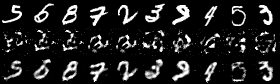
\includegraphics[width=0.7\textwidth]{figures/weakness_rec/MNIST-true-positives.png}}
        }
        \label{fig:true_positives}
    }
    \hspace{5mm}
    \subfloat[Adversarial false negatives.]{%
        \resizebox{0.45\textwidth}{!}{
          \centerline{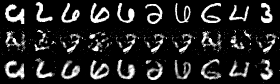
\includegraphics[width=0.7\textwidth]{figures/weakness_rec/MNIST-false-negatives.png}}
        }
        \label{fig:false_negatives}
    }
    \caption{MNIST failure predictions from the adversary.}\label{fig:predictions}
\end{figure*}


\Cref{fig:predictions} compares the failures classified by the adversary.
For the true positives in \Cref{fig:true_positives}, the top row of digits are the $10$ digits with the highest predicted failure likelihood that were true failures, the middle row shows the feature that had the strongest influence on the failure classification (decoding a one-hot vector representation of the maximum of a $\softmax$ over low-dimensional inputs), and the bottom row shows the reconstructed digits after passing through the autoencoder.
Similarly for the false negatives in \Cref{fig:false_negatives}, the top row are the $10$ digits with the lowest predicted failure likelihood that were true failures, the middle row shows the strongest influential feature, and the bottom row shows the output of the autoencoder. Notice that certain features in the middle row are shared among the other digits, indicating features that play a larger role in classifying failures.

\begin{figure*}[ht]
    \centering
    \subfloat[Confusion matrix.]{%
        \resizebox{0.45\textwidth}{!}{%% Creator: Matplotlib, PGF backend
%%
%% To include the figure in your LaTeX document, write
%%   \input{<filename>.pgf}
%%
%% Make sure the required packages are loaded in your preamble
%%   \usepackage{pgf}
%%
%% and, on pdftex
%%   \usepackage[utf8]{inputenc}\DeclareUnicodeCharacter{2212}{-}
%%
%% or, on luatex and xetex
%%   \usepackage{unicode-math}
%%
%% Figures using additional raster images can only be included by \input if
%% they are in the same directory as the main LaTeX file. For loading figures
%% from other directories you can use the `import` package
%%   \usepackage{import}
%%
%% and then include the figures with
%%   \import{<path to file>}{<filename>.pgf}
%%
%% Matplotlib used the following preamble
%%   \usepackage{fontspec}
%%
\begingroup%
\makeatletter%
\begin{pgfpicture}%
\pgfpathrectangle{\pgfpointorigin}{\pgfqpoint{3.724945in}{3.111639in}}%
\pgfusepath{use as bounding box, clip}%
\begin{pgfscope}%
\pgfsetbuttcap%
\pgfsetmiterjoin%
\definecolor{currentfill}{rgb}{1.000000,1.000000,1.000000}%
\pgfsetfillcolor{currentfill}%
\pgfsetlinewidth{0.000000pt}%
\definecolor{currentstroke}{rgb}{1.000000,1.000000,1.000000}%
\pgfsetstrokecolor{currentstroke}%
\pgfsetdash{}{0pt}%
\pgfpathmoveto{\pgfqpoint{0.000000in}{0.000000in}}%
\pgfpathlineto{\pgfqpoint{3.724945in}{0.000000in}}%
\pgfpathlineto{\pgfqpoint{3.724945in}{3.111639in}}%
\pgfpathlineto{\pgfqpoint{0.000000in}{3.111639in}}%
\pgfpathclose%
\pgfusepath{fill}%
\end{pgfscope}%
\begin{pgfscope}%
\pgfsetbuttcap%
\pgfsetmiterjoin%
\definecolor{currentfill}{rgb}{1.000000,1.000000,1.000000}%
\pgfsetfillcolor{currentfill}%
\pgfsetlinewidth{0.000000pt}%
\definecolor{currentstroke}{rgb}{0.000000,0.000000,0.000000}%
\pgfsetstrokecolor{currentstroke}%
\pgfsetstrokeopacity{0.000000}%
\pgfsetdash{}{0pt}%
\pgfpathmoveto{\pgfqpoint{0.499444in}{0.500972in}}%
\pgfpathlineto{\pgfqpoint{2.979444in}{0.500972in}}%
\pgfpathlineto{\pgfqpoint{2.979444in}{2.810972in}}%
\pgfpathlineto{\pgfqpoint{0.499444in}{2.810972in}}%
\pgfpathclose%
\pgfusepath{fill}%
\end{pgfscope}%
\begin{pgfscope}%
\pgfpathrectangle{\pgfqpoint{0.499444in}{0.500972in}}{\pgfqpoint{2.480000in}{2.310000in}}%
\pgfusepath{clip}%
\pgfsetbuttcap%
\pgfsetroundjoin%
\definecolor{currentfill}{rgb}{0.993248,0.906157,0.143936}%
\pgfsetfillcolor{currentfill}%
\pgfsetlinewidth{0.000000pt}%
\definecolor{currentstroke}{rgb}{1.000000,1.000000,1.000000}%
\pgfsetstrokecolor{currentstroke}%
\pgfsetdash{}{0pt}%
\pgfpathmoveto{\pgfqpoint{0.499444in}{2.810972in}}%
\pgfpathlineto{\pgfqpoint{1.739444in}{2.810972in}}%
\pgfpathlineto{\pgfqpoint{1.739444in}{1.655972in}}%
\pgfpathlineto{\pgfqpoint{0.499444in}{1.655972in}}%
\pgfpathlineto{\pgfqpoint{0.499444in}{2.810972in}}%
\pgfusepath{fill}%
\end{pgfscope}%
\begin{pgfscope}%
\pgfpathrectangle{\pgfqpoint{0.499444in}{0.500972in}}{\pgfqpoint{2.480000in}{2.310000in}}%
\pgfusepath{clip}%
\pgfsetbuttcap%
\pgfsetroundjoin%
\definecolor{currentfill}{rgb}{0.277941,0.056324,0.381191}%
\pgfsetfillcolor{currentfill}%
\pgfsetlinewidth{0.000000pt}%
\definecolor{currentstroke}{rgb}{1.000000,1.000000,1.000000}%
\pgfsetstrokecolor{currentstroke}%
\pgfsetdash{}{0pt}%
\pgfpathmoveto{\pgfqpoint{1.739444in}{2.810972in}}%
\pgfpathlineto{\pgfqpoint{2.979444in}{2.810972in}}%
\pgfpathlineto{\pgfqpoint{2.979444in}{1.655972in}}%
\pgfpathlineto{\pgfqpoint{1.739444in}{1.655972in}}%
\pgfpathlineto{\pgfqpoint{1.739444in}{2.810972in}}%
\pgfusepath{fill}%
\end{pgfscope}%
\begin{pgfscope}%
\pgfpathrectangle{\pgfqpoint{0.499444in}{0.500972in}}{\pgfqpoint{2.480000in}{2.310000in}}%
\pgfusepath{clip}%
\pgfsetbuttcap%
\pgfsetroundjoin%
\definecolor{currentfill}{rgb}{0.278791,0.062145,0.386592}%
\pgfsetfillcolor{currentfill}%
\pgfsetlinewidth{0.000000pt}%
\definecolor{currentstroke}{rgb}{1.000000,1.000000,1.000000}%
\pgfsetstrokecolor{currentstroke}%
\pgfsetdash{}{0pt}%
\pgfpathmoveto{\pgfqpoint{0.499444in}{1.655972in}}%
\pgfpathlineto{\pgfqpoint{1.739444in}{1.655972in}}%
\pgfpathlineto{\pgfqpoint{1.739444in}{0.500972in}}%
\pgfpathlineto{\pgfqpoint{0.499444in}{0.500972in}}%
\pgfpathlineto{\pgfqpoint{0.499444in}{1.655972in}}%
\pgfusepath{fill}%
\end{pgfscope}%
\begin{pgfscope}%
\pgfpathrectangle{\pgfqpoint{0.499444in}{0.500972in}}{\pgfqpoint{2.480000in}{2.310000in}}%
\pgfusepath{clip}%
\pgfsetbuttcap%
\pgfsetroundjoin%
\definecolor{currentfill}{rgb}{0.267004,0.004874,0.329415}%
\pgfsetfillcolor{currentfill}%
\pgfsetlinewidth{0.000000pt}%
\definecolor{currentstroke}{rgb}{1.000000,1.000000,1.000000}%
\pgfsetstrokecolor{currentstroke}%
\pgfsetdash{}{0pt}%
\pgfpathmoveto{\pgfqpoint{1.739444in}{1.655972in}}%
\pgfpathlineto{\pgfqpoint{2.979444in}{1.655972in}}%
\pgfpathlineto{\pgfqpoint{2.979444in}{0.500972in}}%
\pgfpathlineto{\pgfqpoint{1.739444in}{0.500972in}}%
\pgfpathlineto{\pgfqpoint{1.739444in}{1.655972in}}%
\pgfusepath{fill}%
\end{pgfscope}%
\begin{pgfscope}%
\pgfsetbuttcap%
\pgfsetroundjoin%
\definecolor{currentfill}{rgb}{0.000000,0.000000,0.000000}%
\pgfsetfillcolor{currentfill}%
\pgfsetlinewidth{0.803000pt}%
\definecolor{currentstroke}{rgb}{0.000000,0.000000,0.000000}%
\pgfsetstrokecolor{currentstroke}%
\pgfsetdash{}{0pt}%
\pgfsys@defobject{currentmarker}{\pgfqpoint{0.000000in}{-0.048611in}}{\pgfqpoint{0.000000in}{0.000000in}}{%
\pgfpathmoveto{\pgfqpoint{0.000000in}{0.000000in}}%
\pgfpathlineto{\pgfqpoint{0.000000in}{-0.048611in}}%
\pgfusepath{stroke,fill}%
}%
\begin{pgfscope}%
\pgfsys@transformshift{1.119444in}{0.500972in}%
\pgfsys@useobject{currentmarker}{}%
\end{pgfscope}%
\end{pgfscope}%
\begin{pgfscope}%
\definecolor{textcolor}{rgb}{0.000000,0.000000,0.000000}%
\pgfsetstrokecolor{textcolor}%
\pgfsetfillcolor{textcolor}%
\pgftext[x=1.119444in,y=0.403750in,,top]{\color{textcolor}\rmfamily\fontsize{10.000000}{12.000000}\selectfont not failure}%
\end{pgfscope}%
\begin{pgfscope}%
\pgfsetbuttcap%
\pgfsetroundjoin%
\definecolor{currentfill}{rgb}{0.000000,0.000000,0.000000}%
\pgfsetfillcolor{currentfill}%
\pgfsetlinewidth{0.803000pt}%
\definecolor{currentstroke}{rgb}{0.000000,0.000000,0.000000}%
\pgfsetstrokecolor{currentstroke}%
\pgfsetdash{}{0pt}%
\pgfsys@defobject{currentmarker}{\pgfqpoint{0.000000in}{-0.048611in}}{\pgfqpoint{0.000000in}{0.000000in}}{%
\pgfpathmoveto{\pgfqpoint{0.000000in}{0.000000in}}%
\pgfpathlineto{\pgfqpoint{0.000000in}{-0.048611in}}%
\pgfusepath{stroke,fill}%
}%
\begin{pgfscope}%
\pgfsys@transformshift{2.359444in}{0.500972in}%
\pgfsys@useobject{currentmarker}{}%
\end{pgfscope}%
\end{pgfscope}%
\begin{pgfscope}%
\definecolor{textcolor}{rgb}{0.000000,0.000000,0.000000}%
\pgfsetstrokecolor{textcolor}%
\pgfsetfillcolor{textcolor}%
\pgftext[x=2.359444in,y=0.403750in,,top]{\color{textcolor}\rmfamily\fontsize{10.000000}{12.000000}\selectfont failure}%
\end{pgfscope}%
\begin{pgfscope}%
\definecolor{textcolor}{rgb}{0.000000,0.000000,0.000000}%
\pgfsetstrokecolor{textcolor}%
\pgfsetfillcolor{textcolor}%
\pgftext[x=1.739444in,y=0.224861in,,top]{\color{textcolor}\rmfamily\fontsize{10.000000}{12.000000}\selectfont predicted failures}%
\end{pgfscope}%
\begin{pgfscope}%
\pgfsetbuttcap%
\pgfsetroundjoin%
\definecolor{currentfill}{rgb}{0.000000,0.000000,0.000000}%
\pgfsetfillcolor{currentfill}%
\pgfsetlinewidth{0.803000pt}%
\definecolor{currentstroke}{rgb}{0.000000,0.000000,0.000000}%
\pgfsetstrokecolor{currentstroke}%
\pgfsetdash{}{0pt}%
\pgfsys@defobject{currentmarker}{\pgfqpoint{-0.048611in}{0.000000in}}{\pgfqpoint{0.000000in}{0.000000in}}{%
\pgfpathmoveto{\pgfqpoint{0.000000in}{0.000000in}}%
\pgfpathlineto{\pgfqpoint{-0.048611in}{0.000000in}}%
\pgfusepath{stroke,fill}%
}%
\begin{pgfscope}%
\pgfsys@transformshift{0.499444in}{2.233472in}%
\pgfsys@useobject{currentmarker}{}%
\end{pgfscope}%
\end{pgfscope}%
\begin{pgfscope}%
\definecolor{textcolor}{rgb}{0.000000,0.000000,0.000000}%
\pgfsetstrokecolor{textcolor}%
\pgfsetfillcolor{textcolor}%
\pgftext[x=0.375278in, y=1.9in, left, base,rotate=90.000000]{\color{textcolor}\rmfamily\fontsize{10.000000}{12.000000}\selectfont not failure}%
\end{pgfscope}%
\begin{pgfscope}%
\pgfsetbuttcap%
\pgfsetroundjoin%
\definecolor{currentfill}{rgb}{0.000000,0.000000,0.000000}%
\pgfsetfillcolor{currentfill}%
\pgfsetlinewidth{0.803000pt}%
\definecolor{currentstroke}{rgb}{0.000000,0.000000,0.000000}%
\pgfsetstrokecolor{currentstroke}%
\pgfsetdash{}{0pt}%
\pgfsys@defobject{currentmarker}{\pgfqpoint{-0.048611in}{0.000000in}}{\pgfqpoint{0.000000in}{0.000000in}}{%
\pgfpathmoveto{\pgfqpoint{0.000000in}{0.000000in}}%
\pgfpathlineto{\pgfqpoint{-0.048611in}{0.000000in}}%
\pgfusepath{stroke,fill}%
}%
\begin{pgfscope}%
\pgfsys@transformshift{0.499444in}{1.078472in}%
\pgfsys@useobject{currentmarker}{}%
\end{pgfscope}%
\end{pgfscope}%
\begin{pgfscope}%
\definecolor{textcolor}{rgb}{0.000000,0.000000,0.000000}%
\pgfsetstrokecolor{textcolor}%
\pgfsetfillcolor{textcolor}%
\pgftext[x=0.375278in, y=0.9in, left, base,rotate=90.000000]{\color{textcolor}\rmfamily\fontsize{10.000000}{12.000000}\selectfont failure}%
\end{pgfscope}%
\begin{pgfscope}%
\definecolor{textcolor}{rgb}{0.000000,0.000000,0.000000}%
\pgfsetstrokecolor{textcolor}%
\pgfsetfillcolor{textcolor}%
\pgftext[x=0.223333in,y=1.655972in,,bottom,rotate=90.000000]{\color{textcolor}\rmfamily\fontsize{10.000000}{12.000000}\selectfont true failures}%
\end{pgfscope}%
\begin{pgfscope}%
\definecolor{textcolor}{rgb}{0.150000,0.150000,0.150000}%
\pgfsetstrokecolor{textcolor}%
\pgfsetfillcolor{textcolor}%
\pgftext[x=1.119444in,y=2.233472in,,]{\color{textcolor}\rmfamily\fontsize{12.000000}{14.400000}\selectfont 8849}%
\end{pgfscope}%
\begin{pgfscope}%
\definecolor{textcolor}{rgb}{1.000000,1.000000,1.000000}%
\pgfsetstrokecolor{textcolor}%
\pgfsetfillcolor{textcolor}%
\pgftext[x=2.359444in,y=2.233472in,,]{\color{textcolor}\rmfamily\fontsize{12.000000}{14.400000}\selectfont 474}%
\end{pgfscope}%
\begin{pgfscope}%
\definecolor{textcolor}{rgb}{1.000000,1.000000,1.000000}%
\pgfsetstrokecolor{textcolor}%
\pgfsetfillcolor{textcolor}%
\pgftext[x=1.119444in,y=1.078472in,,]{\color{textcolor}\rmfamily\fontsize{12.000000}{14.400000}\selectfont 524}%
\end{pgfscope}%
\begin{pgfscope}%
\definecolor{textcolor}{rgb}{1.000000,1.000000,1.000000}%
\pgfsetstrokecolor{textcolor}%
\pgfsetfillcolor{textcolor}%
\pgftext[x=2.359444in,y=1.078472in,,]{\color{textcolor}\rmfamily\fontsize{12.000000}{14.400000}\selectfont 153}%
\end{pgfscope}%
\begin{pgfscope}%
\definecolor{textcolor}{rgb}{0.000000,0.000000,0.000000}%
\pgfsetstrokecolor{textcolor}%
\pgfsetfillcolor{textcolor}%
\pgftext[x=1.739444in,y=2.894305in,,base]{\color{textcolor}\rmfamily\fontsize{12.000000}{14.400000}\selectfont Confusion matrix for adversary \(\displaystyle \mathcal{A}\)}%
\end{pgfscope}%
\begin{pgfscope}%
\pgfpathrectangle{\pgfqpoint{3.134444in}{0.500972in}}{\pgfqpoint{0.115500in}{2.310000in}}%
\pgfusepath{clip}%
\pgfsetbuttcap%
\pgfsetmiterjoin%
\definecolor{currentfill}{rgb}{1.000000,1.000000,1.000000}%
\pgfsetfillcolor{currentfill}%
\pgfsetlinewidth{0.010037pt}%
\definecolor{currentstroke}{rgb}{1.000000,1.000000,1.000000}%
\pgfsetstrokecolor{currentstroke}%
\pgfsetdash{}{0pt}%
\pgfpathmoveto{\pgfqpoint{3.134444in}{0.500972in}}%
\pgfpathlineto{\pgfqpoint{3.134444in}{0.509995in}}%
\pgfpathlineto{\pgfqpoint{3.134444in}{2.801949in}}%
\pgfpathlineto{\pgfqpoint{3.134444in}{2.810972in}}%
\pgfpathlineto{\pgfqpoint{3.249944in}{2.810972in}}%
\pgfpathlineto{\pgfqpoint{3.249944in}{2.801949in}}%
\pgfpathlineto{\pgfqpoint{3.249944in}{0.509995in}}%
\pgfpathlineto{\pgfqpoint{3.249944in}{0.500972in}}%
\pgfpathclose%
\pgfusepath{stroke,fill}%
\end{pgfscope}%
\begin{pgfscope}%
\pgfsys@transformshift{3.130000in}{0.501639in}%
\pgftext[left,bottom]{
\includegraphics[interpolate=true,width=0.120000in,height=2.310000in]{figures/weakness_rec/confusion_adversary-img0.png}}%
\end{pgfscope}%
\begin{pgfscope}%
\pgfsetbuttcap%
\pgfsetroundjoin%
\definecolor{currentfill}{rgb}{0.000000,0.000000,0.000000}%
\pgfsetfillcolor{currentfill}%
\pgfsetlinewidth{0.803000pt}%
\definecolor{currentstroke}{rgb}{0.000000,0.000000,0.000000}%
\pgfsetstrokecolor{currentstroke}%
\pgfsetdash{}{0pt}%
\pgfsys@defobject{currentmarker}{\pgfqpoint{0.000000in}{0.000000in}}{\pgfqpoint{0.048611in}{0.000000in}}{%
\pgfpathmoveto{\pgfqpoint{0.000000in}{0.000000in}}%
\pgfpathlineto{\pgfqpoint{0.048611in}{0.000000in}}%
\pgfusepath{stroke,fill}%
}%
\begin{pgfscope}%
\pgfsys@transformshift{3.249944in}{0.991608in}%
\pgfsys@useobject{currentmarker}{}%
\end{pgfscope}%
\end{pgfscope}%
\begin{pgfscope}%
\definecolor{textcolor}{rgb}{0.000000,0.000000,0.000000}%
\pgfsetstrokecolor{textcolor}%
\pgfsetfillcolor{textcolor}%
\pgftext[x=3.347166in, y=0.943413in, left, base]{\color{textcolor}\rmfamily\fontsize{10.000000}{12.000000}\selectfont \(\displaystyle {2000}\)}%
\end{pgfscope}%
\begin{pgfscope}%
\pgfsetbuttcap%
\pgfsetroundjoin%
\definecolor{currentfill}{rgb}{0.000000,0.000000,0.000000}%
\pgfsetfillcolor{currentfill}%
\pgfsetlinewidth{0.803000pt}%
\definecolor{currentstroke}{rgb}{0.000000,0.000000,0.000000}%
\pgfsetstrokecolor{currentstroke}%
\pgfsetdash{}{0pt}%
\pgfsys@defobject{currentmarker}{\pgfqpoint{0.000000in}{0.000000in}}{\pgfqpoint{0.048611in}{0.000000in}}{%
\pgfpathmoveto{\pgfqpoint{0.000000in}{0.000000in}}%
\pgfpathlineto{\pgfqpoint{0.048611in}{0.000000in}}%
\pgfusepath{stroke,fill}%
}%
\begin{pgfscope}%
\pgfsys@transformshift{3.249944in}{1.522887in}%
\pgfsys@useobject{currentmarker}{}%
\end{pgfscope}%
\end{pgfscope}%
\begin{pgfscope}%
\definecolor{textcolor}{rgb}{0.000000,0.000000,0.000000}%
\pgfsetstrokecolor{textcolor}%
\pgfsetfillcolor{textcolor}%
\pgftext[x=3.347166in, y=1.474692in, left, base]{\color{textcolor}\rmfamily\fontsize{10.000000}{12.000000}\selectfont \(\displaystyle {4000}\)}%
\end{pgfscope}%
\begin{pgfscope}%
\pgfsetbuttcap%
\pgfsetroundjoin%
\definecolor{currentfill}{rgb}{0.000000,0.000000,0.000000}%
\pgfsetfillcolor{currentfill}%
\pgfsetlinewidth{0.803000pt}%
\definecolor{currentstroke}{rgb}{0.000000,0.000000,0.000000}%
\pgfsetstrokecolor{currentstroke}%
\pgfsetdash{}{0pt}%
\pgfsys@defobject{currentmarker}{\pgfqpoint{0.000000in}{0.000000in}}{\pgfqpoint{0.048611in}{0.000000in}}{%
\pgfpathmoveto{\pgfqpoint{0.000000in}{0.000000in}}%
\pgfpathlineto{\pgfqpoint{0.048611in}{0.000000in}}%
\pgfusepath{stroke,fill}%
}%
\begin{pgfscope}%
\pgfsys@transformshift{3.249944in}{2.054165in}%
\pgfsys@useobject{currentmarker}{}%
\end{pgfscope}%
\end{pgfscope}%
\begin{pgfscope}%
\definecolor{textcolor}{rgb}{0.000000,0.000000,0.000000}%
\pgfsetstrokecolor{textcolor}%
\pgfsetfillcolor{textcolor}%
\pgftext[x=3.347166in, y=2.005971in, left, base]{\color{textcolor}\rmfamily\fontsize{10.000000}{12.000000}\selectfont \(\displaystyle {6000}\)}%
\end{pgfscope}%
\begin{pgfscope}%
\pgfsetbuttcap%
\pgfsetroundjoin%
\definecolor{currentfill}{rgb}{0.000000,0.000000,0.000000}%
\pgfsetfillcolor{currentfill}%
\pgfsetlinewidth{0.803000pt}%
\definecolor{currentstroke}{rgb}{0.000000,0.000000,0.000000}%
\pgfsetstrokecolor{currentstroke}%
\pgfsetdash{}{0pt}%
\pgfsys@defobject{currentmarker}{\pgfqpoint{0.000000in}{0.000000in}}{\pgfqpoint{0.048611in}{0.000000in}}{%
\pgfpathmoveto{\pgfqpoint{0.000000in}{0.000000in}}%
\pgfpathlineto{\pgfqpoint{0.048611in}{0.000000in}}%
\pgfusepath{stroke,fill}%
}%
\begin{pgfscope}%
\pgfsys@transformshift{3.249944in}{2.585444in}%
\pgfsys@useobject{currentmarker}{}%
\end{pgfscope}%
\end{pgfscope}%
\begin{pgfscope}%
\definecolor{textcolor}{rgb}{0.000000,0.000000,0.000000}%
\pgfsetstrokecolor{textcolor}%
\pgfsetfillcolor{textcolor}%
\pgftext[x=3.347166in, y=2.537250in, left, base]{\color{textcolor}\rmfamily\fontsize{10.000000}{12.000000}\selectfont \(\displaystyle {8000}\)}%
\end{pgfscope}%
\begin{pgfscope}%
\pgfsetbuttcap%
\pgfsetmiterjoin%
\pgfsetlinewidth{0.000000pt}%
\definecolor{currentstroke}{rgb}{0.000000,0.000000,0.000000}%
\pgfsetstrokecolor{currentstroke}%
\pgfsetdash{}{0pt}%
\pgfpathmoveto{\pgfqpoint{3.134444in}{0.500972in}}%
\pgfpathlineto{\pgfqpoint{3.134444in}{0.509995in}}%
\pgfpathlineto{\pgfqpoint{3.134444in}{2.801949in}}%
\pgfpathlineto{\pgfqpoint{3.134444in}{2.810972in}}%
\pgfpathlineto{\pgfqpoint{3.249944in}{2.810972in}}%
\pgfpathlineto{\pgfqpoint{3.249944in}{2.801949in}}%
\pgfpathlineto{\pgfqpoint{3.249944in}{0.509995in}}%
\pgfpathlineto{\pgfqpoint{3.249944in}{0.500972in}}%
\pgfpathclose%
\pgfusepath{}%
\end{pgfscope}%
\end{pgfpicture}%
\makeatother%
\endgroup%
}
        \label{fig:confusion_adversary}
    }
    \subfloat[Failure likelihood prediction per pixel.]{%
        \resizebox{0.45\textwidth}{!}{%% Creator: Matplotlib, PGF backend
%%
%% To include the figure in your LaTeX document, write
%%   \input{<filename>.pgf}
%%
%% Make sure the required packages are loaded in your preamble
%%   \usepackage{pgf}
%%
%% and, on pdftex
%%   \usepackage[utf8]{inputenc}\DeclareUnicodeCharacter{2212}{-}
%%
%% or, on luatex and xetex
%%   \usepackage{unicode-math}
%%
%% Figures using additional raster images can only be included by \input if
%% they are in the same directory as the main LaTeX file. For loading figures
%% from other directories you can use the `import` package
%%   \usepackage{import}
%%
%% and then include the figures with
%%   \import{<path to file>}{<filename>.pgf}
%%
%% Matplotlib used the following preamble
%%   \usepackage{fontspec}
%%
\begingroup%
\makeatletter%
\begin{pgfpicture}%
\pgfpathrectangle{\pgfpointorigin}{\pgfqpoint{3.640254in}{3.124000in}}%
\pgfusepath{use as bounding box, clip}%
\begin{pgfscope}%
\pgfsetbuttcap%
\pgfsetmiterjoin%
\definecolor{currentfill}{rgb}{1.000000,1.000000,1.000000}%
\pgfsetfillcolor{currentfill}%
\pgfsetlinewidth{0.000000pt}%
\definecolor{currentstroke}{rgb}{1.000000,1.000000,1.000000}%
\pgfsetstrokecolor{currentstroke}%
\pgfsetdash{}{0pt}%
\pgfpathmoveto{\pgfqpoint{0.000000in}{0.000000in}}%
\pgfpathlineto{\pgfqpoint{3.640254in}{0.000000in}}%
\pgfpathlineto{\pgfqpoint{3.640254in}{3.124000in}}%
\pgfpathlineto{\pgfqpoint{0.000000in}{3.124000in}}%
\pgfpathclose%
\pgfusepath{fill}%
\end{pgfscope}%
\begin{pgfscope}%
\pgfsetbuttcap%
\pgfsetmiterjoin%
\definecolor{currentfill}{rgb}{1.000000,1.000000,1.000000}%
\pgfsetfillcolor{currentfill}%
\pgfsetlinewidth{0.000000pt}%
\definecolor{currentstroke}{rgb}{0.000000,0.000000,0.000000}%
\pgfsetstrokecolor{currentstroke}%
\pgfsetstrokeopacity{0.000000}%
\pgfsetdash{}{0pt}%
\pgfpathmoveto{\pgfqpoint{0.515062in}{0.515000in}}%
\pgfpathlineto{\pgfqpoint{2.995062in}{0.515000in}}%
\pgfpathlineto{\pgfqpoint{2.995062in}{2.825000in}}%
\pgfpathlineto{\pgfqpoint{0.515062in}{2.825000in}}%
\pgfpathclose%
\pgfusepath{fill}%
\end{pgfscope}%
\begin{pgfscope}%
\pgfpathrectangle{\pgfqpoint{0.515062in}{0.515000in}}{\pgfqpoint{2.480000in}{2.310000in}}%
\pgfusepath{clip}%
\pgfsetbuttcap%
\pgfsetroundjoin%
\definecolor{currentfill}{rgb}{0.246811,0.283237,0.535941}%
\pgfsetfillcolor{currentfill}%
\pgfsetlinewidth{0.000000pt}%
\definecolor{currentstroke}{rgb}{1.000000,1.000000,1.000000}%
\pgfsetstrokecolor{currentstroke}%
\pgfsetdash{}{0pt}%
\pgfpathmoveto{\pgfqpoint{0.515062in}{2.825000in}}%
\pgfpathlineto{\pgfqpoint{0.603633in}{2.825000in}}%
\pgfpathlineto{\pgfqpoint{0.603633in}{2.742500in}}%
\pgfpathlineto{\pgfqpoint{0.515062in}{2.742500in}}%
\pgfpathlineto{\pgfqpoint{0.515062in}{2.825000in}}%
\pgfusepath{fill}%
\end{pgfscope}%
\begin{pgfscope}%
\pgfpathrectangle{\pgfqpoint{0.515062in}{0.515000in}}{\pgfqpoint{2.480000in}{2.310000in}}%
\pgfusepath{clip}%
\pgfsetbuttcap%
\pgfsetroundjoin%
\definecolor{currentfill}{rgb}{0.258965,0.251537,0.524736}%
\pgfsetfillcolor{currentfill}%
\pgfsetlinewidth{0.000000pt}%
\definecolor{currentstroke}{rgb}{1.000000,1.000000,1.000000}%
\pgfsetstrokecolor{currentstroke}%
\pgfsetdash{}{0pt}%
\pgfpathmoveto{\pgfqpoint{0.603633in}{2.825000in}}%
\pgfpathlineto{\pgfqpoint{0.692205in}{2.825000in}}%
\pgfpathlineto{\pgfqpoint{0.692205in}{2.742500in}}%
\pgfpathlineto{\pgfqpoint{0.603633in}{2.742500in}}%
\pgfpathlineto{\pgfqpoint{0.603633in}{2.825000in}}%
\pgfusepath{fill}%
\end{pgfscope}%
\begin{pgfscope}%
\pgfpathrectangle{\pgfqpoint{0.515062in}{0.515000in}}{\pgfqpoint{2.480000in}{2.310000in}}%
\pgfusepath{clip}%
\pgfsetbuttcap%
\pgfsetroundjoin%
\definecolor{currentfill}{rgb}{0.258965,0.251537,0.524736}%
\pgfsetfillcolor{currentfill}%
\pgfsetlinewidth{0.000000pt}%
\definecolor{currentstroke}{rgb}{1.000000,1.000000,1.000000}%
\pgfsetstrokecolor{currentstroke}%
\pgfsetdash{}{0pt}%
\pgfpathmoveto{\pgfqpoint{0.692205in}{2.825000in}}%
\pgfpathlineto{\pgfqpoint{0.780776in}{2.825000in}}%
\pgfpathlineto{\pgfqpoint{0.780776in}{2.742500in}}%
\pgfpathlineto{\pgfqpoint{0.692205in}{2.742500in}}%
\pgfpathlineto{\pgfqpoint{0.692205in}{2.825000in}}%
\pgfusepath{fill}%
\end{pgfscope}%
\begin{pgfscope}%
\pgfpathrectangle{\pgfqpoint{0.515062in}{0.515000in}}{\pgfqpoint{2.480000in}{2.310000in}}%
\pgfusepath{clip}%
\pgfsetbuttcap%
\pgfsetroundjoin%
\definecolor{currentfill}{rgb}{0.263663,0.237631,0.518762}%
\pgfsetfillcolor{currentfill}%
\pgfsetlinewidth{0.000000pt}%
\definecolor{currentstroke}{rgb}{1.000000,1.000000,1.000000}%
\pgfsetstrokecolor{currentstroke}%
\pgfsetdash{}{0pt}%
\pgfpathmoveto{\pgfqpoint{0.780776in}{2.825000in}}%
\pgfpathlineto{\pgfqpoint{0.869347in}{2.825000in}}%
\pgfpathlineto{\pgfqpoint{0.869347in}{2.742500in}}%
\pgfpathlineto{\pgfqpoint{0.780776in}{2.742500in}}%
\pgfpathlineto{\pgfqpoint{0.780776in}{2.825000in}}%
\pgfusepath{fill}%
\end{pgfscope}%
\begin{pgfscope}%
\pgfpathrectangle{\pgfqpoint{0.515062in}{0.515000in}}{\pgfqpoint{2.480000in}{2.310000in}}%
\pgfusepath{clip}%
\pgfsetbuttcap%
\pgfsetroundjoin%
\definecolor{currentfill}{rgb}{0.187231,0.414746,0.556547}%
\pgfsetfillcolor{currentfill}%
\pgfsetlinewidth{0.000000pt}%
\definecolor{currentstroke}{rgb}{1.000000,1.000000,1.000000}%
\pgfsetstrokecolor{currentstroke}%
\pgfsetdash{}{0pt}%
\pgfpathmoveto{\pgfqpoint{0.869347in}{2.825000in}}%
\pgfpathlineto{\pgfqpoint{0.957919in}{2.825000in}}%
\pgfpathlineto{\pgfqpoint{0.957919in}{2.742500in}}%
\pgfpathlineto{\pgfqpoint{0.869347in}{2.742500in}}%
\pgfpathlineto{\pgfqpoint{0.869347in}{2.825000in}}%
\pgfusepath{fill}%
\end{pgfscope}%
\begin{pgfscope}%
\pgfpathrectangle{\pgfqpoint{0.515062in}{0.515000in}}{\pgfqpoint{2.480000in}{2.310000in}}%
\pgfusepath{clip}%
\pgfsetbuttcap%
\pgfsetroundjoin%
\definecolor{currentfill}{rgb}{0.262138,0.242286,0.520837}%
\pgfsetfillcolor{currentfill}%
\pgfsetlinewidth{0.000000pt}%
\definecolor{currentstroke}{rgb}{1.000000,1.000000,1.000000}%
\pgfsetstrokecolor{currentstroke}%
\pgfsetdash{}{0pt}%
\pgfpathmoveto{\pgfqpoint{0.957919in}{2.825000in}}%
\pgfpathlineto{\pgfqpoint{1.046490in}{2.825000in}}%
\pgfpathlineto{\pgfqpoint{1.046490in}{2.742500in}}%
\pgfpathlineto{\pgfqpoint{0.957919in}{2.742500in}}%
\pgfpathlineto{\pgfqpoint{0.957919in}{2.825000in}}%
\pgfusepath{fill}%
\end{pgfscope}%
\begin{pgfscope}%
\pgfpathrectangle{\pgfqpoint{0.515062in}{0.515000in}}{\pgfqpoint{2.480000in}{2.310000in}}%
\pgfusepath{clip}%
\pgfsetbuttcap%
\pgfsetroundjoin%
\definecolor{currentfill}{rgb}{0.223925,0.334994,0.548053}%
\pgfsetfillcolor{currentfill}%
\pgfsetlinewidth{0.000000pt}%
\definecolor{currentstroke}{rgb}{1.000000,1.000000,1.000000}%
\pgfsetstrokecolor{currentstroke}%
\pgfsetdash{}{0pt}%
\pgfpathmoveto{\pgfqpoint{1.046490in}{2.825000in}}%
\pgfpathlineto{\pgfqpoint{1.135062in}{2.825000in}}%
\pgfpathlineto{\pgfqpoint{1.135062in}{2.742500in}}%
\pgfpathlineto{\pgfqpoint{1.046490in}{2.742500in}}%
\pgfpathlineto{\pgfqpoint{1.046490in}{2.825000in}}%
\pgfusepath{fill}%
\end{pgfscope}%
\begin{pgfscope}%
\pgfpathrectangle{\pgfqpoint{0.515062in}{0.515000in}}{\pgfqpoint{2.480000in}{2.310000in}}%
\pgfusepath{clip}%
\pgfsetbuttcap%
\pgfsetroundjoin%
\definecolor{currentfill}{rgb}{0.250425,0.274290,0.533103}%
\pgfsetfillcolor{currentfill}%
\pgfsetlinewidth{0.000000pt}%
\definecolor{currentstroke}{rgb}{1.000000,1.000000,1.000000}%
\pgfsetstrokecolor{currentstroke}%
\pgfsetdash{}{0pt}%
\pgfpathmoveto{\pgfqpoint{1.135062in}{2.825000in}}%
\pgfpathlineto{\pgfqpoint{1.223633in}{2.825000in}}%
\pgfpathlineto{\pgfqpoint{1.223633in}{2.742500in}}%
\pgfpathlineto{\pgfqpoint{1.135062in}{2.742500in}}%
\pgfpathlineto{\pgfqpoint{1.135062in}{2.825000in}}%
\pgfusepath{fill}%
\end{pgfscope}%
\begin{pgfscope}%
\pgfpathrectangle{\pgfqpoint{0.515062in}{0.515000in}}{\pgfqpoint{2.480000in}{2.310000in}}%
\pgfusepath{clip}%
\pgfsetbuttcap%
\pgfsetroundjoin%
\definecolor{currentfill}{rgb}{0.263663,0.237631,0.518762}%
\pgfsetfillcolor{currentfill}%
\pgfsetlinewidth{0.000000pt}%
\definecolor{currentstroke}{rgb}{1.000000,1.000000,1.000000}%
\pgfsetstrokecolor{currentstroke}%
\pgfsetdash{}{0pt}%
\pgfpathmoveto{\pgfqpoint{1.223633in}{2.825000in}}%
\pgfpathlineto{\pgfqpoint{1.312205in}{2.825000in}}%
\pgfpathlineto{\pgfqpoint{1.312205in}{2.742500in}}%
\pgfpathlineto{\pgfqpoint{1.223633in}{2.742500in}}%
\pgfpathlineto{\pgfqpoint{1.223633in}{2.825000in}}%
\pgfusepath{fill}%
\end{pgfscope}%
\begin{pgfscope}%
\pgfpathrectangle{\pgfqpoint{0.515062in}{0.515000in}}{\pgfqpoint{2.480000in}{2.310000in}}%
\pgfusepath{clip}%
\pgfsetbuttcap%
\pgfsetroundjoin%
\definecolor{currentfill}{rgb}{0.279566,0.067836,0.391917}%
\pgfsetfillcolor{currentfill}%
\pgfsetlinewidth{0.000000pt}%
\definecolor{currentstroke}{rgb}{1.000000,1.000000,1.000000}%
\pgfsetstrokecolor{currentstroke}%
\pgfsetdash{}{0pt}%
\pgfpathmoveto{\pgfqpoint{1.312205in}{2.825000in}}%
\pgfpathlineto{\pgfqpoint{1.400776in}{2.825000in}}%
\pgfpathlineto{\pgfqpoint{1.400776in}{2.742500in}}%
\pgfpathlineto{\pgfqpoint{1.312205in}{2.742500in}}%
\pgfpathlineto{\pgfqpoint{1.312205in}{2.825000in}}%
\pgfusepath{fill}%
\end{pgfscope}%
\begin{pgfscope}%
\pgfpathrectangle{\pgfqpoint{0.515062in}{0.515000in}}{\pgfqpoint{2.480000in}{2.310000in}}%
\pgfusepath{clip}%
\pgfsetbuttcap%
\pgfsetroundjoin%
\definecolor{currentfill}{rgb}{0.277941,0.056324,0.381191}%
\pgfsetfillcolor{currentfill}%
\pgfsetlinewidth{0.000000pt}%
\definecolor{currentstroke}{rgb}{1.000000,1.000000,1.000000}%
\pgfsetstrokecolor{currentstroke}%
\pgfsetdash{}{0pt}%
\pgfpathmoveto{\pgfqpoint{1.400776in}{2.825000in}}%
\pgfpathlineto{\pgfqpoint{1.489347in}{2.825000in}}%
\pgfpathlineto{\pgfqpoint{1.489347in}{2.742500in}}%
\pgfpathlineto{\pgfqpoint{1.400776in}{2.742500in}}%
\pgfpathlineto{\pgfqpoint{1.400776in}{2.825000in}}%
\pgfusepath{fill}%
\end{pgfscope}%
\begin{pgfscope}%
\pgfpathrectangle{\pgfqpoint{0.515062in}{0.515000in}}{\pgfqpoint{2.480000in}{2.310000in}}%
\pgfusepath{clip}%
\pgfsetbuttcap%
\pgfsetroundjoin%
\definecolor{currentfill}{rgb}{0.280868,0.160771,0.472899}%
\pgfsetfillcolor{currentfill}%
\pgfsetlinewidth{0.000000pt}%
\definecolor{currentstroke}{rgb}{1.000000,1.000000,1.000000}%
\pgfsetstrokecolor{currentstroke}%
\pgfsetdash{}{0pt}%
\pgfpathmoveto{\pgfqpoint{1.489347in}{2.825000in}}%
\pgfpathlineto{\pgfqpoint{1.577919in}{2.825000in}}%
\pgfpathlineto{\pgfqpoint{1.577919in}{2.742500in}}%
\pgfpathlineto{\pgfqpoint{1.489347in}{2.742500in}}%
\pgfpathlineto{\pgfqpoint{1.489347in}{2.825000in}}%
\pgfusepath{fill}%
\end{pgfscope}%
\begin{pgfscope}%
\pgfpathrectangle{\pgfqpoint{0.515062in}{0.515000in}}{\pgfqpoint{2.480000in}{2.310000in}}%
\pgfusepath{clip}%
\pgfsetbuttcap%
\pgfsetroundjoin%
\definecolor{currentfill}{rgb}{0.214298,0.355619,0.551184}%
\pgfsetfillcolor{currentfill}%
\pgfsetlinewidth{0.000000pt}%
\definecolor{currentstroke}{rgb}{1.000000,1.000000,1.000000}%
\pgfsetstrokecolor{currentstroke}%
\pgfsetdash{}{0pt}%
\pgfpathmoveto{\pgfqpoint{1.577919in}{2.825000in}}%
\pgfpathlineto{\pgfqpoint{1.666490in}{2.825000in}}%
\pgfpathlineto{\pgfqpoint{1.666490in}{2.742500in}}%
\pgfpathlineto{\pgfqpoint{1.577919in}{2.742500in}}%
\pgfpathlineto{\pgfqpoint{1.577919in}{2.825000in}}%
\pgfusepath{fill}%
\end{pgfscope}%
\begin{pgfscope}%
\pgfpathrectangle{\pgfqpoint{0.515062in}{0.515000in}}{\pgfqpoint{2.480000in}{2.310000in}}%
\pgfusepath{clip}%
\pgfsetbuttcap%
\pgfsetroundjoin%
\definecolor{currentfill}{rgb}{0.250425,0.274290,0.533103}%
\pgfsetfillcolor{currentfill}%
\pgfsetlinewidth{0.000000pt}%
\definecolor{currentstroke}{rgb}{1.000000,1.000000,1.000000}%
\pgfsetstrokecolor{currentstroke}%
\pgfsetdash{}{0pt}%
\pgfpathmoveto{\pgfqpoint{1.666490in}{2.825000in}}%
\pgfpathlineto{\pgfqpoint{1.755062in}{2.825000in}}%
\pgfpathlineto{\pgfqpoint{1.755062in}{2.742500in}}%
\pgfpathlineto{\pgfqpoint{1.666490in}{2.742500in}}%
\pgfpathlineto{\pgfqpoint{1.666490in}{2.825000in}}%
\pgfusepath{fill}%
\end{pgfscope}%
\begin{pgfscope}%
\pgfpathrectangle{\pgfqpoint{0.515062in}{0.515000in}}{\pgfqpoint{2.480000in}{2.310000in}}%
\pgfusepath{clip}%
\pgfsetbuttcap%
\pgfsetroundjoin%
\definecolor{currentfill}{rgb}{0.229739,0.322361,0.545706}%
\pgfsetfillcolor{currentfill}%
\pgfsetlinewidth{0.000000pt}%
\definecolor{currentstroke}{rgb}{1.000000,1.000000,1.000000}%
\pgfsetstrokecolor{currentstroke}%
\pgfsetdash{}{0pt}%
\pgfpathmoveto{\pgfqpoint{1.755062in}{2.825000in}}%
\pgfpathlineto{\pgfqpoint{1.843633in}{2.825000in}}%
\pgfpathlineto{\pgfqpoint{1.843633in}{2.742500in}}%
\pgfpathlineto{\pgfqpoint{1.755062in}{2.742500in}}%
\pgfpathlineto{\pgfqpoint{1.755062in}{2.825000in}}%
\pgfusepath{fill}%
\end{pgfscope}%
\begin{pgfscope}%
\pgfpathrectangle{\pgfqpoint{0.515062in}{0.515000in}}{\pgfqpoint{2.480000in}{2.310000in}}%
\pgfusepath{clip}%
\pgfsetbuttcap%
\pgfsetroundjoin%
\definecolor{currentfill}{rgb}{0.269308,0.218818,0.509577}%
\pgfsetfillcolor{currentfill}%
\pgfsetlinewidth{0.000000pt}%
\definecolor{currentstroke}{rgb}{1.000000,1.000000,1.000000}%
\pgfsetstrokecolor{currentstroke}%
\pgfsetdash{}{0pt}%
\pgfpathmoveto{\pgfqpoint{1.843633in}{2.825000in}}%
\pgfpathlineto{\pgfqpoint{1.932205in}{2.825000in}}%
\pgfpathlineto{\pgfqpoint{1.932205in}{2.742500in}}%
\pgfpathlineto{\pgfqpoint{1.843633in}{2.742500in}}%
\pgfpathlineto{\pgfqpoint{1.843633in}{2.825000in}}%
\pgfusepath{fill}%
\end{pgfscope}%
\begin{pgfscope}%
\pgfpathrectangle{\pgfqpoint{0.515062in}{0.515000in}}{\pgfqpoint{2.480000in}{2.310000in}}%
\pgfusepath{clip}%
\pgfsetbuttcap%
\pgfsetroundjoin%
\definecolor{currentfill}{rgb}{0.266580,0.228262,0.514349}%
\pgfsetfillcolor{currentfill}%
\pgfsetlinewidth{0.000000pt}%
\definecolor{currentstroke}{rgb}{1.000000,1.000000,1.000000}%
\pgfsetstrokecolor{currentstroke}%
\pgfsetdash{}{0pt}%
\pgfpathmoveto{\pgfqpoint{1.932205in}{2.825000in}}%
\pgfpathlineto{\pgfqpoint{2.020776in}{2.825000in}}%
\pgfpathlineto{\pgfqpoint{2.020776in}{2.742500in}}%
\pgfpathlineto{\pgfqpoint{1.932205in}{2.742500in}}%
\pgfpathlineto{\pgfqpoint{1.932205in}{2.825000in}}%
\pgfusepath{fill}%
\end{pgfscope}%
\begin{pgfscope}%
\pgfpathrectangle{\pgfqpoint{0.515062in}{0.515000in}}{\pgfqpoint{2.480000in}{2.310000in}}%
\pgfusepath{clip}%
\pgfsetbuttcap%
\pgfsetroundjoin%
\definecolor{currentfill}{rgb}{0.216210,0.351535,0.550627}%
\pgfsetfillcolor{currentfill}%
\pgfsetlinewidth{0.000000pt}%
\definecolor{currentstroke}{rgb}{1.000000,1.000000,1.000000}%
\pgfsetstrokecolor{currentstroke}%
\pgfsetdash{}{0pt}%
\pgfpathmoveto{\pgfqpoint{2.020776in}{2.825000in}}%
\pgfpathlineto{\pgfqpoint{2.109347in}{2.825000in}}%
\pgfpathlineto{\pgfqpoint{2.109347in}{2.742500in}}%
\pgfpathlineto{\pgfqpoint{2.020776in}{2.742500in}}%
\pgfpathlineto{\pgfqpoint{2.020776in}{2.825000in}}%
\pgfusepath{fill}%
\end{pgfscope}%
\begin{pgfscope}%
\pgfpathrectangle{\pgfqpoint{0.515062in}{0.515000in}}{\pgfqpoint{2.480000in}{2.310000in}}%
\pgfusepath{clip}%
\pgfsetbuttcap%
\pgfsetroundjoin%
\definecolor{currentfill}{rgb}{0.267968,0.223549,0.512008}%
\pgfsetfillcolor{currentfill}%
\pgfsetlinewidth{0.000000pt}%
\definecolor{currentstroke}{rgb}{1.000000,1.000000,1.000000}%
\pgfsetstrokecolor{currentstroke}%
\pgfsetdash{}{0pt}%
\pgfpathmoveto{\pgfqpoint{2.109347in}{2.825000in}}%
\pgfpathlineto{\pgfqpoint{2.197919in}{2.825000in}}%
\pgfpathlineto{\pgfqpoint{2.197919in}{2.742500in}}%
\pgfpathlineto{\pgfqpoint{2.109347in}{2.742500in}}%
\pgfpathlineto{\pgfqpoint{2.109347in}{2.825000in}}%
\pgfusepath{fill}%
\end{pgfscope}%
\begin{pgfscope}%
\pgfpathrectangle{\pgfqpoint{0.515062in}{0.515000in}}{\pgfqpoint{2.480000in}{2.310000in}}%
\pgfusepath{clip}%
\pgfsetbuttcap%
\pgfsetroundjoin%
\definecolor{currentfill}{rgb}{0.218130,0.347432,0.550038}%
\pgfsetfillcolor{currentfill}%
\pgfsetlinewidth{0.000000pt}%
\definecolor{currentstroke}{rgb}{1.000000,1.000000,1.000000}%
\pgfsetstrokecolor{currentstroke}%
\pgfsetdash{}{0pt}%
\pgfpathmoveto{\pgfqpoint{2.197919in}{2.825000in}}%
\pgfpathlineto{\pgfqpoint{2.286490in}{2.825000in}}%
\pgfpathlineto{\pgfqpoint{2.286490in}{2.742500in}}%
\pgfpathlineto{\pgfqpoint{2.197919in}{2.742500in}}%
\pgfpathlineto{\pgfqpoint{2.197919in}{2.825000in}}%
\pgfusepath{fill}%
\end{pgfscope}%
\begin{pgfscope}%
\pgfpathrectangle{\pgfqpoint{0.515062in}{0.515000in}}{\pgfqpoint{2.480000in}{2.310000in}}%
\pgfusepath{clip}%
\pgfsetbuttcap%
\pgfsetroundjoin%
\definecolor{currentfill}{rgb}{0.257322,0.256130,0.526563}%
\pgfsetfillcolor{currentfill}%
\pgfsetlinewidth{0.000000pt}%
\definecolor{currentstroke}{rgb}{1.000000,1.000000,1.000000}%
\pgfsetstrokecolor{currentstroke}%
\pgfsetdash{}{0pt}%
\pgfpathmoveto{\pgfqpoint{2.286490in}{2.825000in}}%
\pgfpathlineto{\pgfqpoint{2.375062in}{2.825000in}}%
\pgfpathlineto{\pgfqpoint{2.375062in}{2.742500in}}%
\pgfpathlineto{\pgfqpoint{2.286490in}{2.742500in}}%
\pgfpathlineto{\pgfqpoint{2.286490in}{2.825000in}}%
\pgfusepath{fill}%
\end{pgfscope}%
\begin{pgfscope}%
\pgfpathrectangle{\pgfqpoint{0.515062in}{0.515000in}}{\pgfqpoint{2.480000in}{2.310000in}}%
\pgfusepath{clip}%
\pgfsetbuttcap%
\pgfsetroundjoin%
\definecolor{currentfill}{rgb}{0.265145,0.232956,0.516599}%
\pgfsetfillcolor{currentfill}%
\pgfsetlinewidth{0.000000pt}%
\definecolor{currentstroke}{rgb}{1.000000,1.000000,1.000000}%
\pgfsetstrokecolor{currentstroke}%
\pgfsetdash{}{0pt}%
\pgfpathmoveto{\pgfqpoint{2.375062in}{2.825000in}}%
\pgfpathlineto{\pgfqpoint{2.463633in}{2.825000in}}%
\pgfpathlineto{\pgfqpoint{2.463633in}{2.742500in}}%
\pgfpathlineto{\pgfqpoint{2.375062in}{2.742500in}}%
\pgfpathlineto{\pgfqpoint{2.375062in}{2.825000in}}%
\pgfusepath{fill}%
\end{pgfscope}%
\begin{pgfscope}%
\pgfpathrectangle{\pgfqpoint{0.515062in}{0.515000in}}{\pgfqpoint{2.480000in}{2.310000in}}%
\pgfusepath{clip}%
\pgfsetbuttcap%
\pgfsetroundjoin%
\definecolor{currentfill}{rgb}{0.274128,0.199721,0.498911}%
\pgfsetfillcolor{currentfill}%
\pgfsetlinewidth{0.000000pt}%
\definecolor{currentstroke}{rgb}{1.000000,1.000000,1.000000}%
\pgfsetstrokecolor{currentstroke}%
\pgfsetdash{}{0pt}%
\pgfpathmoveto{\pgfqpoint{2.463633in}{2.825000in}}%
\pgfpathlineto{\pgfqpoint{2.552205in}{2.825000in}}%
\pgfpathlineto{\pgfqpoint{2.552205in}{2.742500in}}%
\pgfpathlineto{\pgfqpoint{2.463633in}{2.742500in}}%
\pgfpathlineto{\pgfqpoint{2.463633in}{2.825000in}}%
\pgfusepath{fill}%
\end{pgfscope}%
\begin{pgfscope}%
\pgfpathrectangle{\pgfqpoint{0.515062in}{0.515000in}}{\pgfqpoint{2.480000in}{2.310000in}}%
\pgfusepath{clip}%
\pgfsetbuttcap%
\pgfsetroundjoin%
\definecolor{currentfill}{rgb}{0.273006,0.204520,0.501721}%
\pgfsetfillcolor{currentfill}%
\pgfsetlinewidth{0.000000pt}%
\definecolor{currentstroke}{rgb}{1.000000,1.000000,1.000000}%
\pgfsetstrokecolor{currentstroke}%
\pgfsetdash{}{0pt}%
\pgfpathmoveto{\pgfqpoint{2.552205in}{2.825000in}}%
\pgfpathlineto{\pgfqpoint{2.640776in}{2.825000in}}%
\pgfpathlineto{\pgfqpoint{2.640776in}{2.742500in}}%
\pgfpathlineto{\pgfqpoint{2.552205in}{2.742500in}}%
\pgfpathlineto{\pgfqpoint{2.552205in}{2.825000in}}%
\pgfusepath{fill}%
\end{pgfscope}%
\begin{pgfscope}%
\pgfpathrectangle{\pgfqpoint{0.515062in}{0.515000in}}{\pgfqpoint{2.480000in}{2.310000in}}%
\pgfusepath{clip}%
\pgfsetbuttcap%
\pgfsetroundjoin%
\definecolor{currentfill}{rgb}{0.195860,0.395433,0.555276}%
\pgfsetfillcolor{currentfill}%
\pgfsetlinewidth{0.000000pt}%
\definecolor{currentstroke}{rgb}{1.000000,1.000000,1.000000}%
\pgfsetstrokecolor{currentstroke}%
\pgfsetdash{}{0pt}%
\pgfpathmoveto{\pgfqpoint{2.640776in}{2.825000in}}%
\pgfpathlineto{\pgfqpoint{2.729347in}{2.825000in}}%
\pgfpathlineto{\pgfqpoint{2.729347in}{2.742500in}}%
\pgfpathlineto{\pgfqpoint{2.640776in}{2.742500in}}%
\pgfpathlineto{\pgfqpoint{2.640776in}{2.825000in}}%
\pgfusepath{fill}%
\end{pgfscope}%
\begin{pgfscope}%
\pgfpathrectangle{\pgfqpoint{0.515062in}{0.515000in}}{\pgfqpoint{2.480000in}{2.310000in}}%
\pgfusepath{clip}%
\pgfsetbuttcap%
\pgfsetroundjoin%
\definecolor{currentfill}{rgb}{0.227802,0.326594,0.546532}%
\pgfsetfillcolor{currentfill}%
\pgfsetlinewidth{0.000000pt}%
\definecolor{currentstroke}{rgb}{1.000000,1.000000,1.000000}%
\pgfsetstrokecolor{currentstroke}%
\pgfsetdash{}{0pt}%
\pgfpathmoveto{\pgfqpoint{2.729347in}{2.825000in}}%
\pgfpathlineto{\pgfqpoint{2.817919in}{2.825000in}}%
\pgfpathlineto{\pgfqpoint{2.817919in}{2.742500in}}%
\pgfpathlineto{\pgfqpoint{2.729347in}{2.742500in}}%
\pgfpathlineto{\pgfqpoint{2.729347in}{2.825000in}}%
\pgfusepath{fill}%
\end{pgfscope}%
\begin{pgfscope}%
\pgfpathrectangle{\pgfqpoint{0.515062in}{0.515000in}}{\pgfqpoint{2.480000in}{2.310000in}}%
\pgfusepath{clip}%
\pgfsetbuttcap%
\pgfsetroundjoin%
\definecolor{currentfill}{rgb}{0.260571,0.246922,0.522828}%
\pgfsetfillcolor{currentfill}%
\pgfsetlinewidth{0.000000pt}%
\definecolor{currentstroke}{rgb}{1.000000,1.000000,1.000000}%
\pgfsetstrokecolor{currentstroke}%
\pgfsetdash{}{0pt}%
\pgfpathmoveto{\pgfqpoint{2.817919in}{2.825000in}}%
\pgfpathlineto{\pgfqpoint{2.906490in}{2.825000in}}%
\pgfpathlineto{\pgfqpoint{2.906490in}{2.742500in}}%
\pgfpathlineto{\pgfqpoint{2.817919in}{2.742500in}}%
\pgfpathlineto{\pgfqpoint{2.817919in}{2.825000in}}%
\pgfusepath{fill}%
\end{pgfscope}%
\begin{pgfscope}%
\pgfpathrectangle{\pgfqpoint{0.515062in}{0.515000in}}{\pgfqpoint{2.480000in}{2.310000in}}%
\pgfusepath{clip}%
\pgfsetbuttcap%
\pgfsetroundjoin%
\definecolor{currentfill}{rgb}{0.223925,0.334994,0.548053}%
\pgfsetfillcolor{currentfill}%
\pgfsetlinewidth{0.000000pt}%
\definecolor{currentstroke}{rgb}{1.000000,1.000000,1.000000}%
\pgfsetstrokecolor{currentstroke}%
\pgfsetdash{}{0pt}%
\pgfpathmoveto{\pgfqpoint{2.906490in}{2.825000in}}%
\pgfpathlineto{\pgfqpoint{2.995062in}{2.825000in}}%
\pgfpathlineto{\pgfqpoint{2.995062in}{2.742500in}}%
\pgfpathlineto{\pgfqpoint{2.906490in}{2.742500in}}%
\pgfpathlineto{\pgfqpoint{2.906490in}{2.825000in}}%
\pgfusepath{fill}%
\end{pgfscope}%
\begin{pgfscope}%
\pgfpathrectangle{\pgfqpoint{0.515062in}{0.515000in}}{\pgfqpoint{2.480000in}{2.310000in}}%
\pgfusepath{clip}%
\pgfsetbuttcap%
\pgfsetroundjoin%
\definecolor{currentfill}{rgb}{0.274128,0.199721,0.498911}%
\pgfsetfillcolor{currentfill}%
\pgfsetlinewidth{0.000000pt}%
\definecolor{currentstroke}{rgb}{1.000000,1.000000,1.000000}%
\pgfsetstrokecolor{currentstroke}%
\pgfsetdash{}{0pt}%
\pgfpathmoveto{\pgfqpoint{0.515062in}{2.742500in}}%
\pgfpathlineto{\pgfqpoint{0.603633in}{2.742500in}}%
\pgfpathlineto{\pgfqpoint{0.603633in}{2.660000in}}%
\pgfpathlineto{\pgfqpoint{0.515062in}{2.660000in}}%
\pgfpathlineto{\pgfqpoint{0.515062in}{2.742500in}}%
\pgfusepath{fill}%
\end{pgfscope}%
\begin{pgfscope}%
\pgfpathrectangle{\pgfqpoint{0.515062in}{0.515000in}}{\pgfqpoint{2.480000in}{2.310000in}}%
\pgfusepath{clip}%
\pgfsetbuttcap%
\pgfsetroundjoin%
\definecolor{currentfill}{rgb}{0.260571,0.246922,0.522828}%
\pgfsetfillcolor{currentfill}%
\pgfsetlinewidth{0.000000pt}%
\definecolor{currentstroke}{rgb}{1.000000,1.000000,1.000000}%
\pgfsetstrokecolor{currentstroke}%
\pgfsetdash{}{0pt}%
\pgfpathmoveto{\pgfqpoint{0.603633in}{2.742500in}}%
\pgfpathlineto{\pgfqpoint{0.692205in}{2.742500in}}%
\pgfpathlineto{\pgfqpoint{0.692205in}{2.660000in}}%
\pgfpathlineto{\pgfqpoint{0.603633in}{2.660000in}}%
\pgfpathlineto{\pgfqpoint{0.603633in}{2.742500in}}%
\pgfusepath{fill}%
\end{pgfscope}%
\begin{pgfscope}%
\pgfpathrectangle{\pgfqpoint{0.515062in}{0.515000in}}{\pgfqpoint{2.480000in}{2.310000in}}%
\pgfusepath{clip}%
\pgfsetbuttcap%
\pgfsetroundjoin%
\definecolor{currentfill}{rgb}{0.210503,0.363727,0.552206}%
\pgfsetfillcolor{currentfill}%
\pgfsetlinewidth{0.000000pt}%
\definecolor{currentstroke}{rgb}{1.000000,1.000000,1.000000}%
\pgfsetstrokecolor{currentstroke}%
\pgfsetdash{}{0pt}%
\pgfpathmoveto{\pgfqpoint{0.692205in}{2.742500in}}%
\pgfpathlineto{\pgfqpoint{0.780776in}{2.742500in}}%
\pgfpathlineto{\pgfqpoint{0.780776in}{2.660000in}}%
\pgfpathlineto{\pgfqpoint{0.692205in}{2.660000in}}%
\pgfpathlineto{\pgfqpoint{0.692205in}{2.742500in}}%
\pgfusepath{fill}%
\end{pgfscope}%
\begin{pgfscope}%
\pgfpathrectangle{\pgfqpoint{0.515062in}{0.515000in}}{\pgfqpoint{2.480000in}{2.310000in}}%
\pgfusepath{clip}%
\pgfsetbuttcap%
\pgfsetroundjoin%
\definecolor{currentfill}{rgb}{0.248629,0.278775,0.534556}%
\pgfsetfillcolor{currentfill}%
\pgfsetlinewidth{0.000000pt}%
\definecolor{currentstroke}{rgb}{1.000000,1.000000,1.000000}%
\pgfsetstrokecolor{currentstroke}%
\pgfsetdash{}{0pt}%
\pgfpathmoveto{\pgfqpoint{0.780776in}{2.742500in}}%
\pgfpathlineto{\pgfqpoint{0.869347in}{2.742500in}}%
\pgfpathlineto{\pgfqpoint{0.869347in}{2.660000in}}%
\pgfpathlineto{\pgfqpoint{0.780776in}{2.660000in}}%
\pgfpathlineto{\pgfqpoint{0.780776in}{2.742500in}}%
\pgfusepath{fill}%
\end{pgfscope}%
\begin{pgfscope}%
\pgfpathrectangle{\pgfqpoint{0.515062in}{0.515000in}}{\pgfqpoint{2.480000in}{2.310000in}}%
\pgfusepath{clip}%
\pgfsetbuttcap%
\pgfsetroundjoin%
\definecolor{currentfill}{rgb}{0.235526,0.309527,0.542944}%
\pgfsetfillcolor{currentfill}%
\pgfsetlinewidth{0.000000pt}%
\definecolor{currentstroke}{rgb}{1.000000,1.000000,1.000000}%
\pgfsetstrokecolor{currentstroke}%
\pgfsetdash{}{0pt}%
\pgfpathmoveto{\pgfqpoint{0.869347in}{2.742500in}}%
\pgfpathlineto{\pgfqpoint{0.957919in}{2.742500in}}%
\pgfpathlineto{\pgfqpoint{0.957919in}{2.660000in}}%
\pgfpathlineto{\pgfqpoint{0.869347in}{2.660000in}}%
\pgfpathlineto{\pgfqpoint{0.869347in}{2.742500in}}%
\pgfusepath{fill}%
\end{pgfscope}%
\begin{pgfscope}%
\pgfpathrectangle{\pgfqpoint{0.515062in}{0.515000in}}{\pgfqpoint{2.480000in}{2.310000in}}%
\pgfusepath{clip}%
\pgfsetbuttcap%
\pgfsetroundjoin%
\definecolor{currentfill}{rgb}{0.243113,0.292092,0.538516}%
\pgfsetfillcolor{currentfill}%
\pgfsetlinewidth{0.000000pt}%
\definecolor{currentstroke}{rgb}{1.000000,1.000000,1.000000}%
\pgfsetstrokecolor{currentstroke}%
\pgfsetdash{}{0pt}%
\pgfpathmoveto{\pgfqpoint{0.957919in}{2.742500in}}%
\pgfpathlineto{\pgfqpoint{1.046490in}{2.742500in}}%
\pgfpathlineto{\pgfqpoint{1.046490in}{2.660000in}}%
\pgfpathlineto{\pgfqpoint{0.957919in}{2.660000in}}%
\pgfpathlineto{\pgfqpoint{0.957919in}{2.742500in}}%
\pgfusepath{fill}%
\end{pgfscope}%
\begin{pgfscope}%
\pgfpathrectangle{\pgfqpoint{0.515062in}{0.515000in}}{\pgfqpoint{2.480000in}{2.310000in}}%
\pgfusepath{clip}%
\pgfsetbuttcap%
\pgfsetroundjoin%
\definecolor{currentfill}{rgb}{0.258965,0.251537,0.524736}%
\pgfsetfillcolor{currentfill}%
\pgfsetlinewidth{0.000000pt}%
\definecolor{currentstroke}{rgb}{1.000000,1.000000,1.000000}%
\pgfsetstrokecolor{currentstroke}%
\pgfsetdash{}{0pt}%
\pgfpathmoveto{\pgfqpoint{1.046490in}{2.742500in}}%
\pgfpathlineto{\pgfqpoint{1.135062in}{2.742500in}}%
\pgfpathlineto{\pgfqpoint{1.135062in}{2.660000in}}%
\pgfpathlineto{\pgfqpoint{1.046490in}{2.660000in}}%
\pgfpathlineto{\pgfqpoint{1.046490in}{2.742500in}}%
\pgfusepath{fill}%
\end{pgfscope}%
\begin{pgfscope}%
\pgfpathrectangle{\pgfqpoint{0.515062in}{0.515000in}}{\pgfqpoint{2.480000in}{2.310000in}}%
\pgfusepath{clip}%
\pgfsetbuttcap%
\pgfsetroundjoin%
\definecolor{currentfill}{rgb}{0.206756,0.371758,0.553117}%
\pgfsetfillcolor{currentfill}%
\pgfsetlinewidth{0.000000pt}%
\definecolor{currentstroke}{rgb}{1.000000,1.000000,1.000000}%
\pgfsetstrokecolor{currentstroke}%
\pgfsetdash{}{0pt}%
\pgfpathmoveto{\pgfqpoint{1.135062in}{2.742500in}}%
\pgfpathlineto{\pgfqpoint{1.223633in}{2.742500in}}%
\pgfpathlineto{\pgfqpoint{1.223633in}{2.660000in}}%
\pgfpathlineto{\pgfqpoint{1.135062in}{2.660000in}}%
\pgfpathlineto{\pgfqpoint{1.135062in}{2.742500in}}%
\pgfusepath{fill}%
\end{pgfscope}%
\begin{pgfscope}%
\pgfpathrectangle{\pgfqpoint{0.515062in}{0.515000in}}{\pgfqpoint{2.480000in}{2.310000in}}%
\pgfusepath{clip}%
\pgfsetbuttcap%
\pgfsetroundjoin%
\definecolor{currentfill}{rgb}{0.278012,0.180367,0.486697}%
\pgfsetfillcolor{currentfill}%
\pgfsetlinewidth{0.000000pt}%
\definecolor{currentstroke}{rgb}{1.000000,1.000000,1.000000}%
\pgfsetstrokecolor{currentstroke}%
\pgfsetdash{}{0pt}%
\pgfpathmoveto{\pgfqpoint{1.223633in}{2.742500in}}%
\pgfpathlineto{\pgfqpoint{1.312205in}{2.742500in}}%
\pgfpathlineto{\pgfqpoint{1.312205in}{2.660000in}}%
\pgfpathlineto{\pgfqpoint{1.223633in}{2.660000in}}%
\pgfpathlineto{\pgfqpoint{1.223633in}{2.742500in}}%
\pgfusepath{fill}%
\end{pgfscope}%
\begin{pgfscope}%
\pgfpathrectangle{\pgfqpoint{0.515062in}{0.515000in}}{\pgfqpoint{2.480000in}{2.310000in}}%
\pgfusepath{clip}%
\pgfsetbuttcap%
\pgfsetroundjoin%
\definecolor{currentfill}{rgb}{0.252194,0.269783,0.531579}%
\pgfsetfillcolor{currentfill}%
\pgfsetlinewidth{0.000000pt}%
\definecolor{currentstroke}{rgb}{1.000000,1.000000,1.000000}%
\pgfsetstrokecolor{currentstroke}%
\pgfsetdash{}{0pt}%
\pgfpathmoveto{\pgfqpoint{1.312205in}{2.742500in}}%
\pgfpathlineto{\pgfqpoint{1.400776in}{2.742500in}}%
\pgfpathlineto{\pgfqpoint{1.400776in}{2.660000in}}%
\pgfpathlineto{\pgfqpoint{1.312205in}{2.660000in}}%
\pgfpathlineto{\pgfqpoint{1.312205in}{2.742500in}}%
\pgfusepath{fill}%
\end{pgfscope}%
\begin{pgfscope}%
\pgfpathrectangle{\pgfqpoint{0.515062in}{0.515000in}}{\pgfqpoint{2.480000in}{2.310000in}}%
\pgfusepath{clip}%
\pgfsetbuttcap%
\pgfsetroundjoin%
\definecolor{currentfill}{rgb}{0.281446,0.084320,0.407414}%
\pgfsetfillcolor{currentfill}%
\pgfsetlinewidth{0.000000pt}%
\definecolor{currentstroke}{rgb}{1.000000,1.000000,1.000000}%
\pgfsetstrokecolor{currentstroke}%
\pgfsetdash{}{0pt}%
\pgfpathmoveto{\pgfqpoint{1.400776in}{2.742500in}}%
\pgfpathlineto{\pgfqpoint{1.489347in}{2.742500in}}%
\pgfpathlineto{\pgfqpoint{1.489347in}{2.660000in}}%
\pgfpathlineto{\pgfqpoint{1.400776in}{2.660000in}}%
\pgfpathlineto{\pgfqpoint{1.400776in}{2.742500in}}%
\pgfusepath{fill}%
\end{pgfscope}%
\begin{pgfscope}%
\pgfpathrectangle{\pgfqpoint{0.515062in}{0.515000in}}{\pgfqpoint{2.480000in}{2.310000in}}%
\pgfusepath{clip}%
\pgfsetbuttcap%
\pgfsetroundjoin%
\definecolor{currentfill}{rgb}{0.280255,0.165693,0.476498}%
\pgfsetfillcolor{currentfill}%
\pgfsetlinewidth{0.000000pt}%
\definecolor{currentstroke}{rgb}{1.000000,1.000000,1.000000}%
\pgfsetstrokecolor{currentstroke}%
\pgfsetdash{}{0pt}%
\pgfpathmoveto{\pgfqpoint{1.489347in}{2.742500in}}%
\pgfpathlineto{\pgfqpoint{1.577919in}{2.742500in}}%
\pgfpathlineto{\pgfqpoint{1.577919in}{2.660000in}}%
\pgfpathlineto{\pgfqpoint{1.489347in}{2.660000in}}%
\pgfpathlineto{\pgfqpoint{1.489347in}{2.742500in}}%
\pgfusepath{fill}%
\end{pgfscope}%
\begin{pgfscope}%
\pgfpathrectangle{\pgfqpoint{0.515062in}{0.515000in}}{\pgfqpoint{2.480000in}{2.310000in}}%
\pgfusepath{clip}%
\pgfsetbuttcap%
\pgfsetroundjoin%
\definecolor{currentfill}{rgb}{0.125394,0.574318,0.549086}%
\pgfsetfillcolor{currentfill}%
\pgfsetlinewidth{0.000000pt}%
\definecolor{currentstroke}{rgb}{1.000000,1.000000,1.000000}%
\pgfsetstrokecolor{currentstroke}%
\pgfsetdash{}{0pt}%
\pgfpathmoveto{\pgfqpoint{1.577919in}{2.742500in}}%
\pgfpathlineto{\pgfqpoint{1.666490in}{2.742500in}}%
\pgfpathlineto{\pgfqpoint{1.666490in}{2.660000in}}%
\pgfpathlineto{\pgfqpoint{1.577919in}{2.660000in}}%
\pgfpathlineto{\pgfqpoint{1.577919in}{2.742500in}}%
\pgfusepath{fill}%
\end{pgfscope}%
\begin{pgfscope}%
\pgfpathrectangle{\pgfqpoint{0.515062in}{0.515000in}}{\pgfqpoint{2.480000in}{2.310000in}}%
\pgfusepath{clip}%
\pgfsetbuttcap%
\pgfsetroundjoin%
\definecolor{currentfill}{rgb}{0.241237,0.296485,0.539709}%
\pgfsetfillcolor{currentfill}%
\pgfsetlinewidth{0.000000pt}%
\definecolor{currentstroke}{rgb}{1.000000,1.000000,1.000000}%
\pgfsetstrokecolor{currentstroke}%
\pgfsetdash{}{0pt}%
\pgfpathmoveto{\pgfqpoint{1.666490in}{2.742500in}}%
\pgfpathlineto{\pgfqpoint{1.755062in}{2.742500in}}%
\pgfpathlineto{\pgfqpoint{1.755062in}{2.660000in}}%
\pgfpathlineto{\pgfqpoint{1.666490in}{2.660000in}}%
\pgfpathlineto{\pgfqpoint{1.666490in}{2.742500in}}%
\pgfusepath{fill}%
\end{pgfscope}%
\begin{pgfscope}%
\pgfpathrectangle{\pgfqpoint{0.515062in}{0.515000in}}{\pgfqpoint{2.480000in}{2.310000in}}%
\pgfusepath{clip}%
\pgfsetbuttcap%
\pgfsetroundjoin%
\definecolor{currentfill}{rgb}{0.229739,0.322361,0.545706}%
\pgfsetfillcolor{currentfill}%
\pgfsetlinewidth{0.000000pt}%
\definecolor{currentstroke}{rgb}{1.000000,1.000000,1.000000}%
\pgfsetstrokecolor{currentstroke}%
\pgfsetdash{}{0pt}%
\pgfpathmoveto{\pgfqpoint{1.755062in}{2.742500in}}%
\pgfpathlineto{\pgfqpoint{1.843633in}{2.742500in}}%
\pgfpathlineto{\pgfqpoint{1.843633in}{2.660000in}}%
\pgfpathlineto{\pgfqpoint{1.755062in}{2.660000in}}%
\pgfpathlineto{\pgfqpoint{1.755062in}{2.742500in}}%
\pgfusepath{fill}%
\end{pgfscope}%
\begin{pgfscope}%
\pgfpathrectangle{\pgfqpoint{0.515062in}{0.515000in}}{\pgfqpoint{2.480000in}{2.310000in}}%
\pgfusepath{clip}%
\pgfsetbuttcap%
\pgfsetroundjoin%
\definecolor{currentfill}{rgb}{0.233603,0.313828,0.543914}%
\pgfsetfillcolor{currentfill}%
\pgfsetlinewidth{0.000000pt}%
\definecolor{currentstroke}{rgb}{1.000000,1.000000,1.000000}%
\pgfsetstrokecolor{currentstroke}%
\pgfsetdash{}{0pt}%
\pgfpathmoveto{\pgfqpoint{1.843633in}{2.742500in}}%
\pgfpathlineto{\pgfqpoint{1.932205in}{2.742500in}}%
\pgfpathlineto{\pgfqpoint{1.932205in}{2.660000in}}%
\pgfpathlineto{\pgfqpoint{1.843633in}{2.660000in}}%
\pgfpathlineto{\pgfqpoint{1.843633in}{2.742500in}}%
\pgfusepath{fill}%
\end{pgfscope}%
\begin{pgfscope}%
\pgfpathrectangle{\pgfqpoint{0.515062in}{0.515000in}}{\pgfqpoint{2.480000in}{2.310000in}}%
\pgfusepath{clip}%
\pgfsetbuttcap%
\pgfsetroundjoin%
\definecolor{currentfill}{rgb}{0.147607,0.511733,0.557049}%
\pgfsetfillcolor{currentfill}%
\pgfsetlinewidth{0.000000pt}%
\definecolor{currentstroke}{rgb}{1.000000,1.000000,1.000000}%
\pgfsetstrokecolor{currentstroke}%
\pgfsetdash{}{0pt}%
\pgfpathmoveto{\pgfqpoint{1.932205in}{2.742500in}}%
\pgfpathlineto{\pgfqpoint{2.020776in}{2.742500in}}%
\pgfpathlineto{\pgfqpoint{2.020776in}{2.660000in}}%
\pgfpathlineto{\pgfqpoint{1.932205in}{2.660000in}}%
\pgfpathlineto{\pgfqpoint{1.932205in}{2.742500in}}%
\pgfusepath{fill}%
\end{pgfscope}%
\begin{pgfscope}%
\pgfpathrectangle{\pgfqpoint{0.515062in}{0.515000in}}{\pgfqpoint{2.480000in}{2.310000in}}%
\pgfusepath{clip}%
\pgfsetbuttcap%
\pgfsetroundjoin%
\definecolor{currentfill}{rgb}{0.263663,0.237631,0.518762}%
\pgfsetfillcolor{currentfill}%
\pgfsetlinewidth{0.000000pt}%
\definecolor{currentstroke}{rgb}{1.000000,1.000000,1.000000}%
\pgfsetstrokecolor{currentstroke}%
\pgfsetdash{}{0pt}%
\pgfpathmoveto{\pgfqpoint{2.020776in}{2.742500in}}%
\pgfpathlineto{\pgfqpoint{2.109347in}{2.742500in}}%
\pgfpathlineto{\pgfqpoint{2.109347in}{2.660000in}}%
\pgfpathlineto{\pgfqpoint{2.020776in}{2.660000in}}%
\pgfpathlineto{\pgfqpoint{2.020776in}{2.742500in}}%
\pgfusepath{fill}%
\end{pgfscope}%
\begin{pgfscope}%
\pgfpathrectangle{\pgfqpoint{0.515062in}{0.515000in}}{\pgfqpoint{2.480000in}{2.310000in}}%
\pgfusepath{clip}%
\pgfsetbuttcap%
\pgfsetroundjoin%
\definecolor{currentfill}{rgb}{0.229739,0.322361,0.545706}%
\pgfsetfillcolor{currentfill}%
\pgfsetlinewidth{0.000000pt}%
\definecolor{currentstroke}{rgb}{1.000000,1.000000,1.000000}%
\pgfsetstrokecolor{currentstroke}%
\pgfsetdash{}{0pt}%
\pgfpathmoveto{\pgfqpoint{2.109347in}{2.742500in}}%
\pgfpathlineto{\pgfqpoint{2.197919in}{2.742500in}}%
\pgfpathlineto{\pgfqpoint{2.197919in}{2.660000in}}%
\pgfpathlineto{\pgfqpoint{2.109347in}{2.660000in}}%
\pgfpathlineto{\pgfqpoint{2.109347in}{2.742500in}}%
\pgfusepath{fill}%
\end{pgfscope}%
\begin{pgfscope}%
\pgfpathrectangle{\pgfqpoint{0.515062in}{0.515000in}}{\pgfqpoint{2.480000in}{2.310000in}}%
\pgfusepath{clip}%
\pgfsetbuttcap%
\pgfsetroundjoin%
\definecolor{currentfill}{rgb}{0.274128,0.199721,0.498911}%
\pgfsetfillcolor{currentfill}%
\pgfsetlinewidth{0.000000pt}%
\definecolor{currentstroke}{rgb}{1.000000,1.000000,1.000000}%
\pgfsetstrokecolor{currentstroke}%
\pgfsetdash{}{0pt}%
\pgfpathmoveto{\pgfqpoint{2.197919in}{2.742500in}}%
\pgfpathlineto{\pgfqpoint{2.286490in}{2.742500in}}%
\pgfpathlineto{\pgfqpoint{2.286490in}{2.660000in}}%
\pgfpathlineto{\pgfqpoint{2.197919in}{2.660000in}}%
\pgfpathlineto{\pgfqpoint{2.197919in}{2.742500in}}%
\pgfusepath{fill}%
\end{pgfscope}%
\begin{pgfscope}%
\pgfpathrectangle{\pgfqpoint{0.515062in}{0.515000in}}{\pgfqpoint{2.480000in}{2.310000in}}%
\pgfusepath{clip}%
\pgfsetbuttcap%
\pgfsetroundjoin%
\definecolor{currentfill}{rgb}{0.265145,0.232956,0.516599}%
\pgfsetfillcolor{currentfill}%
\pgfsetlinewidth{0.000000pt}%
\definecolor{currentstroke}{rgb}{1.000000,1.000000,1.000000}%
\pgfsetstrokecolor{currentstroke}%
\pgfsetdash{}{0pt}%
\pgfpathmoveto{\pgfqpoint{2.286490in}{2.742500in}}%
\pgfpathlineto{\pgfqpoint{2.375062in}{2.742500in}}%
\pgfpathlineto{\pgfqpoint{2.375062in}{2.660000in}}%
\pgfpathlineto{\pgfqpoint{2.286490in}{2.660000in}}%
\pgfpathlineto{\pgfqpoint{2.286490in}{2.742500in}}%
\pgfusepath{fill}%
\end{pgfscope}%
\begin{pgfscope}%
\pgfpathrectangle{\pgfqpoint{0.515062in}{0.515000in}}{\pgfqpoint{2.480000in}{2.310000in}}%
\pgfusepath{clip}%
\pgfsetbuttcap%
\pgfsetroundjoin%
\definecolor{currentfill}{rgb}{0.175841,0.441290,0.557685}%
\pgfsetfillcolor{currentfill}%
\pgfsetlinewidth{0.000000pt}%
\definecolor{currentstroke}{rgb}{1.000000,1.000000,1.000000}%
\pgfsetstrokecolor{currentstroke}%
\pgfsetdash{}{0pt}%
\pgfpathmoveto{\pgfqpoint{2.375062in}{2.742500in}}%
\pgfpathlineto{\pgfqpoint{2.463633in}{2.742500in}}%
\pgfpathlineto{\pgfqpoint{2.463633in}{2.660000in}}%
\pgfpathlineto{\pgfqpoint{2.375062in}{2.660000in}}%
\pgfpathlineto{\pgfqpoint{2.375062in}{2.742500in}}%
\pgfusepath{fill}%
\end{pgfscope}%
\begin{pgfscope}%
\pgfpathrectangle{\pgfqpoint{0.515062in}{0.515000in}}{\pgfqpoint{2.480000in}{2.310000in}}%
\pgfusepath{clip}%
\pgfsetbuttcap%
\pgfsetroundjoin%
\definecolor{currentfill}{rgb}{0.235526,0.309527,0.542944}%
\pgfsetfillcolor{currentfill}%
\pgfsetlinewidth{0.000000pt}%
\definecolor{currentstroke}{rgb}{1.000000,1.000000,1.000000}%
\pgfsetstrokecolor{currentstroke}%
\pgfsetdash{}{0pt}%
\pgfpathmoveto{\pgfqpoint{2.463633in}{2.742500in}}%
\pgfpathlineto{\pgfqpoint{2.552205in}{2.742500in}}%
\pgfpathlineto{\pgfqpoint{2.552205in}{2.660000in}}%
\pgfpathlineto{\pgfqpoint{2.463633in}{2.660000in}}%
\pgfpathlineto{\pgfqpoint{2.463633in}{2.742500in}}%
\pgfusepath{fill}%
\end{pgfscope}%
\begin{pgfscope}%
\pgfpathrectangle{\pgfqpoint{0.515062in}{0.515000in}}{\pgfqpoint{2.480000in}{2.310000in}}%
\pgfusepath{clip}%
\pgfsetbuttcap%
\pgfsetroundjoin%
\definecolor{currentfill}{rgb}{0.225863,0.330805,0.547314}%
\pgfsetfillcolor{currentfill}%
\pgfsetlinewidth{0.000000pt}%
\definecolor{currentstroke}{rgb}{1.000000,1.000000,1.000000}%
\pgfsetstrokecolor{currentstroke}%
\pgfsetdash{}{0pt}%
\pgfpathmoveto{\pgfqpoint{2.552205in}{2.742500in}}%
\pgfpathlineto{\pgfqpoint{2.640776in}{2.742500in}}%
\pgfpathlineto{\pgfqpoint{2.640776in}{2.660000in}}%
\pgfpathlineto{\pgfqpoint{2.552205in}{2.660000in}}%
\pgfpathlineto{\pgfqpoint{2.552205in}{2.742500in}}%
\pgfusepath{fill}%
\end{pgfscope}%
\begin{pgfscope}%
\pgfpathrectangle{\pgfqpoint{0.515062in}{0.515000in}}{\pgfqpoint{2.480000in}{2.310000in}}%
\pgfusepath{clip}%
\pgfsetbuttcap%
\pgfsetroundjoin%
\definecolor{currentfill}{rgb}{0.276194,0.190074,0.493001}%
\pgfsetfillcolor{currentfill}%
\pgfsetlinewidth{0.000000pt}%
\definecolor{currentstroke}{rgb}{1.000000,1.000000,1.000000}%
\pgfsetstrokecolor{currentstroke}%
\pgfsetdash{}{0pt}%
\pgfpathmoveto{\pgfqpoint{2.640776in}{2.742500in}}%
\pgfpathlineto{\pgfqpoint{2.729347in}{2.742500in}}%
\pgfpathlineto{\pgfqpoint{2.729347in}{2.660000in}}%
\pgfpathlineto{\pgfqpoint{2.640776in}{2.660000in}}%
\pgfpathlineto{\pgfqpoint{2.640776in}{2.742500in}}%
\pgfusepath{fill}%
\end{pgfscope}%
\begin{pgfscope}%
\pgfpathrectangle{\pgfqpoint{0.515062in}{0.515000in}}{\pgfqpoint{2.480000in}{2.310000in}}%
\pgfusepath{clip}%
\pgfsetbuttcap%
\pgfsetroundjoin%
\definecolor{currentfill}{rgb}{0.231674,0.318106,0.544834}%
\pgfsetfillcolor{currentfill}%
\pgfsetlinewidth{0.000000pt}%
\definecolor{currentstroke}{rgb}{1.000000,1.000000,1.000000}%
\pgfsetstrokecolor{currentstroke}%
\pgfsetdash{}{0pt}%
\pgfpathmoveto{\pgfqpoint{2.729347in}{2.742500in}}%
\pgfpathlineto{\pgfqpoint{2.817919in}{2.742500in}}%
\pgfpathlineto{\pgfqpoint{2.817919in}{2.660000in}}%
\pgfpathlineto{\pgfqpoint{2.729347in}{2.660000in}}%
\pgfpathlineto{\pgfqpoint{2.729347in}{2.742500in}}%
\pgfusepath{fill}%
\end{pgfscope}%
\begin{pgfscope}%
\pgfpathrectangle{\pgfqpoint{0.515062in}{0.515000in}}{\pgfqpoint{2.480000in}{2.310000in}}%
\pgfusepath{clip}%
\pgfsetbuttcap%
\pgfsetroundjoin%
\definecolor{currentfill}{rgb}{0.250425,0.274290,0.533103}%
\pgfsetfillcolor{currentfill}%
\pgfsetlinewidth{0.000000pt}%
\definecolor{currentstroke}{rgb}{1.000000,1.000000,1.000000}%
\pgfsetstrokecolor{currentstroke}%
\pgfsetdash{}{0pt}%
\pgfpathmoveto{\pgfqpoint{2.817919in}{2.742500in}}%
\pgfpathlineto{\pgfqpoint{2.906490in}{2.742500in}}%
\pgfpathlineto{\pgfqpoint{2.906490in}{2.660000in}}%
\pgfpathlineto{\pgfqpoint{2.817919in}{2.660000in}}%
\pgfpathlineto{\pgfqpoint{2.817919in}{2.742500in}}%
\pgfusepath{fill}%
\end{pgfscope}%
\begin{pgfscope}%
\pgfpathrectangle{\pgfqpoint{0.515062in}{0.515000in}}{\pgfqpoint{2.480000in}{2.310000in}}%
\pgfusepath{clip}%
\pgfsetbuttcap%
\pgfsetroundjoin%
\definecolor{currentfill}{rgb}{0.225863,0.330805,0.547314}%
\pgfsetfillcolor{currentfill}%
\pgfsetlinewidth{0.000000pt}%
\definecolor{currentstroke}{rgb}{1.000000,1.000000,1.000000}%
\pgfsetstrokecolor{currentstroke}%
\pgfsetdash{}{0pt}%
\pgfpathmoveto{\pgfqpoint{2.906490in}{2.742500in}}%
\pgfpathlineto{\pgfqpoint{2.995062in}{2.742500in}}%
\pgfpathlineto{\pgfqpoint{2.995062in}{2.660000in}}%
\pgfpathlineto{\pgfqpoint{2.906490in}{2.660000in}}%
\pgfpathlineto{\pgfqpoint{2.906490in}{2.742500in}}%
\pgfusepath{fill}%
\end{pgfscope}%
\begin{pgfscope}%
\pgfpathrectangle{\pgfqpoint{0.515062in}{0.515000in}}{\pgfqpoint{2.480000in}{2.310000in}}%
\pgfusepath{clip}%
\pgfsetbuttcap%
\pgfsetroundjoin%
\definecolor{currentfill}{rgb}{0.270595,0.214069,0.507052}%
\pgfsetfillcolor{currentfill}%
\pgfsetlinewidth{0.000000pt}%
\definecolor{currentstroke}{rgb}{1.000000,1.000000,1.000000}%
\pgfsetstrokecolor{currentstroke}%
\pgfsetdash{}{0pt}%
\pgfpathmoveto{\pgfqpoint{0.515062in}{2.660000in}}%
\pgfpathlineto{\pgfqpoint{0.603633in}{2.660000in}}%
\pgfpathlineto{\pgfqpoint{0.603633in}{2.577500in}}%
\pgfpathlineto{\pgfqpoint{0.515062in}{2.577500in}}%
\pgfpathlineto{\pgfqpoint{0.515062in}{2.660000in}}%
\pgfusepath{fill}%
\end{pgfscope}%
\begin{pgfscope}%
\pgfpathrectangle{\pgfqpoint{0.515062in}{0.515000in}}{\pgfqpoint{2.480000in}{2.310000in}}%
\pgfusepath{clip}%
\pgfsetbuttcap%
\pgfsetroundjoin%
\definecolor{currentfill}{rgb}{0.273006,0.204520,0.501721}%
\pgfsetfillcolor{currentfill}%
\pgfsetlinewidth{0.000000pt}%
\definecolor{currentstroke}{rgb}{1.000000,1.000000,1.000000}%
\pgfsetstrokecolor{currentstroke}%
\pgfsetdash{}{0pt}%
\pgfpathmoveto{\pgfqpoint{0.603633in}{2.660000in}}%
\pgfpathlineto{\pgfqpoint{0.692205in}{2.660000in}}%
\pgfpathlineto{\pgfqpoint{0.692205in}{2.577500in}}%
\pgfpathlineto{\pgfqpoint{0.603633in}{2.577500in}}%
\pgfpathlineto{\pgfqpoint{0.603633in}{2.660000in}}%
\pgfusepath{fill}%
\end{pgfscope}%
\begin{pgfscope}%
\pgfpathrectangle{\pgfqpoint{0.515062in}{0.515000in}}{\pgfqpoint{2.480000in}{2.310000in}}%
\pgfusepath{clip}%
\pgfsetbuttcap%
\pgfsetroundjoin%
\definecolor{currentfill}{rgb}{0.223925,0.334994,0.548053}%
\pgfsetfillcolor{currentfill}%
\pgfsetlinewidth{0.000000pt}%
\definecolor{currentstroke}{rgb}{1.000000,1.000000,1.000000}%
\pgfsetstrokecolor{currentstroke}%
\pgfsetdash{}{0pt}%
\pgfpathmoveto{\pgfqpoint{0.692205in}{2.660000in}}%
\pgfpathlineto{\pgfqpoint{0.780776in}{2.660000in}}%
\pgfpathlineto{\pgfqpoint{0.780776in}{2.577500in}}%
\pgfpathlineto{\pgfqpoint{0.692205in}{2.577500in}}%
\pgfpathlineto{\pgfqpoint{0.692205in}{2.660000in}}%
\pgfusepath{fill}%
\end{pgfscope}%
\begin{pgfscope}%
\pgfpathrectangle{\pgfqpoint{0.515062in}{0.515000in}}{\pgfqpoint{2.480000in}{2.310000in}}%
\pgfusepath{clip}%
\pgfsetbuttcap%
\pgfsetroundjoin%
\definecolor{currentfill}{rgb}{0.227802,0.326594,0.546532}%
\pgfsetfillcolor{currentfill}%
\pgfsetlinewidth{0.000000pt}%
\definecolor{currentstroke}{rgb}{1.000000,1.000000,1.000000}%
\pgfsetstrokecolor{currentstroke}%
\pgfsetdash{}{0pt}%
\pgfpathmoveto{\pgfqpoint{0.780776in}{2.660000in}}%
\pgfpathlineto{\pgfqpoint{0.869347in}{2.660000in}}%
\pgfpathlineto{\pgfqpoint{0.869347in}{2.577500in}}%
\pgfpathlineto{\pgfqpoint{0.780776in}{2.577500in}}%
\pgfpathlineto{\pgfqpoint{0.780776in}{2.660000in}}%
\pgfusepath{fill}%
\end{pgfscope}%
\begin{pgfscope}%
\pgfpathrectangle{\pgfqpoint{0.515062in}{0.515000in}}{\pgfqpoint{2.480000in}{2.310000in}}%
\pgfusepath{clip}%
\pgfsetbuttcap%
\pgfsetroundjoin%
\definecolor{currentfill}{rgb}{0.267968,0.223549,0.512008}%
\pgfsetfillcolor{currentfill}%
\pgfsetlinewidth{0.000000pt}%
\definecolor{currentstroke}{rgb}{1.000000,1.000000,1.000000}%
\pgfsetstrokecolor{currentstroke}%
\pgfsetdash{}{0pt}%
\pgfpathmoveto{\pgfqpoint{0.869347in}{2.660000in}}%
\pgfpathlineto{\pgfqpoint{0.957919in}{2.660000in}}%
\pgfpathlineto{\pgfqpoint{0.957919in}{2.577500in}}%
\pgfpathlineto{\pgfqpoint{0.869347in}{2.577500in}}%
\pgfpathlineto{\pgfqpoint{0.869347in}{2.660000in}}%
\pgfusepath{fill}%
\end{pgfscope}%
\begin{pgfscope}%
\pgfpathrectangle{\pgfqpoint{0.515062in}{0.515000in}}{\pgfqpoint{2.480000in}{2.310000in}}%
\pgfusepath{clip}%
\pgfsetbuttcap%
\pgfsetroundjoin%
\definecolor{currentfill}{rgb}{0.221989,0.339161,0.548752}%
\pgfsetfillcolor{currentfill}%
\pgfsetlinewidth{0.000000pt}%
\definecolor{currentstroke}{rgb}{1.000000,1.000000,1.000000}%
\pgfsetstrokecolor{currentstroke}%
\pgfsetdash{}{0pt}%
\pgfpathmoveto{\pgfqpoint{0.957919in}{2.660000in}}%
\pgfpathlineto{\pgfqpoint{1.046490in}{2.660000in}}%
\pgfpathlineto{\pgfqpoint{1.046490in}{2.577500in}}%
\pgfpathlineto{\pgfqpoint{0.957919in}{2.577500in}}%
\pgfpathlineto{\pgfqpoint{0.957919in}{2.660000in}}%
\pgfusepath{fill}%
\end{pgfscope}%
\begin{pgfscope}%
\pgfpathrectangle{\pgfqpoint{0.515062in}{0.515000in}}{\pgfqpoint{2.480000in}{2.310000in}}%
\pgfusepath{clip}%
\pgfsetbuttcap%
\pgfsetroundjoin%
\definecolor{currentfill}{rgb}{0.258965,0.251537,0.524736}%
\pgfsetfillcolor{currentfill}%
\pgfsetlinewidth{0.000000pt}%
\definecolor{currentstroke}{rgb}{1.000000,1.000000,1.000000}%
\pgfsetstrokecolor{currentstroke}%
\pgfsetdash{}{0pt}%
\pgfpathmoveto{\pgfqpoint{1.046490in}{2.660000in}}%
\pgfpathlineto{\pgfqpoint{1.135062in}{2.660000in}}%
\pgfpathlineto{\pgfqpoint{1.135062in}{2.577500in}}%
\pgfpathlineto{\pgfqpoint{1.046490in}{2.577500in}}%
\pgfpathlineto{\pgfqpoint{1.046490in}{2.660000in}}%
\pgfusepath{fill}%
\end{pgfscope}%
\begin{pgfscope}%
\pgfpathrectangle{\pgfqpoint{0.515062in}{0.515000in}}{\pgfqpoint{2.480000in}{2.310000in}}%
\pgfusepath{clip}%
\pgfsetbuttcap%
\pgfsetroundjoin%
\definecolor{currentfill}{rgb}{0.124780,0.640461,0.527068}%
\pgfsetfillcolor{currentfill}%
\pgfsetlinewidth{0.000000pt}%
\definecolor{currentstroke}{rgb}{1.000000,1.000000,1.000000}%
\pgfsetstrokecolor{currentstroke}%
\pgfsetdash{}{0pt}%
\pgfpathmoveto{\pgfqpoint{1.135062in}{2.660000in}}%
\pgfpathlineto{\pgfqpoint{1.223633in}{2.660000in}}%
\pgfpathlineto{\pgfqpoint{1.223633in}{2.577500in}}%
\pgfpathlineto{\pgfqpoint{1.135062in}{2.577500in}}%
\pgfpathlineto{\pgfqpoint{1.135062in}{2.660000in}}%
\pgfusepath{fill}%
\end{pgfscope}%
\begin{pgfscope}%
\pgfpathrectangle{\pgfqpoint{0.515062in}{0.515000in}}{\pgfqpoint{2.480000in}{2.310000in}}%
\pgfusepath{clip}%
\pgfsetbuttcap%
\pgfsetroundjoin%
\definecolor{currentfill}{rgb}{0.283229,0.120777,0.440584}%
\pgfsetfillcolor{currentfill}%
\pgfsetlinewidth{0.000000pt}%
\definecolor{currentstroke}{rgb}{1.000000,1.000000,1.000000}%
\pgfsetstrokecolor{currentstroke}%
\pgfsetdash{}{0pt}%
\pgfpathmoveto{\pgfqpoint{1.223633in}{2.660000in}}%
\pgfpathlineto{\pgfqpoint{1.312205in}{2.660000in}}%
\pgfpathlineto{\pgfqpoint{1.312205in}{2.577500in}}%
\pgfpathlineto{\pgfqpoint{1.223633in}{2.577500in}}%
\pgfpathlineto{\pgfqpoint{1.223633in}{2.660000in}}%
\pgfusepath{fill}%
\end{pgfscope}%
\begin{pgfscope}%
\pgfpathrectangle{\pgfqpoint{0.515062in}{0.515000in}}{\pgfqpoint{2.480000in}{2.310000in}}%
\pgfusepath{clip}%
\pgfsetbuttcap%
\pgfsetroundjoin%
\definecolor{currentfill}{rgb}{0.281887,0.150881,0.465405}%
\pgfsetfillcolor{currentfill}%
\pgfsetlinewidth{0.000000pt}%
\definecolor{currentstroke}{rgb}{1.000000,1.000000,1.000000}%
\pgfsetstrokecolor{currentstroke}%
\pgfsetdash{}{0pt}%
\pgfpathmoveto{\pgfqpoint{1.312205in}{2.660000in}}%
\pgfpathlineto{\pgfqpoint{1.400776in}{2.660000in}}%
\pgfpathlineto{\pgfqpoint{1.400776in}{2.577500in}}%
\pgfpathlineto{\pgfqpoint{1.312205in}{2.577500in}}%
\pgfpathlineto{\pgfqpoint{1.312205in}{2.660000in}}%
\pgfusepath{fill}%
\end{pgfscope}%
\begin{pgfscope}%
\pgfpathrectangle{\pgfqpoint{0.515062in}{0.515000in}}{\pgfqpoint{2.480000in}{2.310000in}}%
\pgfusepath{clip}%
\pgfsetbuttcap%
\pgfsetroundjoin%
\definecolor{currentfill}{rgb}{0.183898,0.422383,0.556944}%
\pgfsetfillcolor{currentfill}%
\pgfsetlinewidth{0.000000pt}%
\definecolor{currentstroke}{rgb}{1.000000,1.000000,1.000000}%
\pgfsetstrokecolor{currentstroke}%
\pgfsetdash{}{0pt}%
\pgfpathmoveto{\pgfqpoint{1.400776in}{2.660000in}}%
\pgfpathlineto{\pgfqpoint{1.489347in}{2.660000in}}%
\pgfpathlineto{\pgfqpoint{1.489347in}{2.577500in}}%
\pgfpathlineto{\pgfqpoint{1.400776in}{2.577500in}}%
\pgfpathlineto{\pgfqpoint{1.400776in}{2.660000in}}%
\pgfusepath{fill}%
\end{pgfscope}%
\begin{pgfscope}%
\pgfpathrectangle{\pgfqpoint{0.515062in}{0.515000in}}{\pgfqpoint{2.480000in}{2.310000in}}%
\pgfusepath{clip}%
\pgfsetbuttcap%
\pgfsetroundjoin%
\definecolor{currentfill}{rgb}{0.212395,0.359683,0.551710}%
\pgfsetfillcolor{currentfill}%
\pgfsetlinewidth{0.000000pt}%
\definecolor{currentstroke}{rgb}{1.000000,1.000000,1.000000}%
\pgfsetstrokecolor{currentstroke}%
\pgfsetdash{}{0pt}%
\pgfpathmoveto{\pgfqpoint{1.489347in}{2.660000in}}%
\pgfpathlineto{\pgfqpoint{1.577919in}{2.660000in}}%
\pgfpathlineto{\pgfqpoint{1.577919in}{2.577500in}}%
\pgfpathlineto{\pgfqpoint{1.489347in}{2.577500in}}%
\pgfpathlineto{\pgfqpoint{1.489347in}{2.660000in}}%
\pgfusepath{fill}%
\end{pgfscope}%
\begin{pgfscope}%
\pgfpathrectangle{\pgfqpoint{0.515062in}{0.515000in}}{\pgfqpoint{2.480000in}{2.310000in}}%
\pgfusepath{clip}%
\pgfsetbuttcap%
\pgfsetroundjoin%
\definecolor{currentfill}{rgb}{0.218130,0.347432,0.550038}%
\pgfsetfillcolor{currentfill}%
\pgfsetlinewidth{0.000000pt}%
\definecolor{currentstroke}{rgb}{1.000000,1.000000,1.000000}%
\pgfsetstrokecolor{currentstroke}%
\pgfsetdash{}{0pt}%
\pgfpathmoveto{\pgfqpoint{1.577919in}{2.660000in}}%
\pgfpathlineto{\pgfqpoint{1.666490in}{2.660000in}}%
\pgfpathlineto{\pgfqpoint{1.666490in}{2.577500in}}%
\pgfpathlineto{\pgfqpoint{1.577919in}{2.577500in}}%
\pgfpathlineto{\pgfqpoint{1.577919in}{2.660000in}}%
\pgfusepath{fill}%
\end{pgfscope}%
\begin{pgfscope}%
\pgfpathrectangle{\pgfqpoint{0.515062in}{0.515000in}}{\pgfqpoint{2.480000in}{2.310000in}}%
\pgfusepath{clip}%
\pgfsetbuttcap%
\pgfsetroundjoin%
\definecolor{currentfill}{rgb}{0.218130,0.347432,0.550038}%
\pgfsetfillcolor{currentfill}%
\pgfsetlinewidth{0.000000pt}%
\definecolor{currentstroke}{rgb}{1.000000,1.000000,1.000000}%
\pgfsetstrokecolor{currentstroke}%
\pgfsetdash{}{0pt}%
\pgfpathmoveto{\pgfqpoint{1.666490in}{2.660000in}}%
\pgfpathlineto{\pgfqpoint{1.755062in}{2.660000in}}%
\pgfpathlineto{\pgfqpoint{1.755062in}{2.577500in}}%
\pgfpathlineto{\pgfqpoint{1.666490in}{2.577500in}}%
\pgfpathlineto{\pgfqpoint{1.666490in}{2.660000in}}%
\pgfusepath{fill}%
\end{pgfscope}%
\begin{pgfscope}%
\pgfpathrectangle{\pgfqpoint{0.515062in}{0.515000in}}{\pgfqpoint{2.480000in}{2.310000in}}%
\pgfusepath{clip}%
\pgfsetbuttcap%
\pgfsetroundjoin%
\definecolor{currentfill}{rgb}{0.204903,0.375746,0.553533}%
\pgfsetfillcolor{currentfill}%
\pgfsetlinewidth{0.000000pt}%
\definecolor{currentstroke}{rgb}{1.000000,1.000000,1.000000}%
\pgfsetstrokecolor{currentstroke}%
\pgfsetdash{}{0pt}%
\pgfpathmoveto{\pgfqpoint{1.755062in}{2.660000in}}%
\pgfpathlineto{\pgfqpoint{1.843633in}{2.660000in}}%
\pgfpathlineto{\pgfqpoint{1.843633in}{2.577500in}}%
\pgfpathlineto{\pgfqpoint{1.755062in}{2.577500in}}%
\pgfpathlineto{\pgfqpoint{1.755062in}{2.660000in}}%
\pgfusepath{fill}%
\end{pgfscope}%
\begin{pgfscope}%
\pgfpathrectangle{\pgfqpoint{0.515062in}{0.515000in}}{\pgfqpoint{2.480000in}{2.310000in}}%
\pgfusepath{clip}%
\pgfsetbuttcap%
\pgfsetroundjoin%
\definecolor{currentfill}{rgb}{0.262138,0.242286,0.520837}%
\pgfsetfillcolor{currentfill}%
\pgfsetlinewidth{0.000000pt}%
\definecolor{currentstroke}{rgb}{1.000000,1.000000,1.000000}%
\pgfsetstrokecolor{currentstroke}%
\pgfsetdash{}{0pt}%
\pgfpathmoveto{\pgfqpoint{1.843633in}{2.660000in}}%
\pgfpathlineto{\pgfqpoint{1.932205in}{2.660000in}}%
\pgfpathlineto{\pgfqpoint{1.932205in}{2.577500in}}%
\pgfpathlineto{\pgfqpoint{1.843633in}{2.577500in}}%
\pgfpathlineto{\pgfqpoint{1.843633in}{2.660000in}}%
\pgfusepath{fill}%
\end{pgfscope}%
\begin{pgfscope}%
\pgfpathrectangle{\pgfqpoint{0.515062in}{0.515000in}}{\pgfqpoint{2.480000in}{2.310000in}}%
\pgfusepath{clip}%
\pgfsetbuttcap%
\pgfsetroundjoin%
\definecolor{currentfill}{rgb}{0.281887,0.150881,0.465405}%
\pgfsetfillcolor{currentfill}%
\pgfsetlinewidth{0.000000pt}%
\definecolor{currentstroke}{rgb}{1.000000,1.000000,1.000000}%
\pgfsetstrokecolor{currentstroke}%
\pgfsetdash{}{0pt}%
\pgfpathmoveto{\pgfqpoint{1.932205in}{2.660000in}}%
\pgfpathlineto{\pgfqpoint{2.020776in}{2.660000in}}%
\pgfpathlineto{\pgfqpoint{2.020776in}{2.577500in}}%
\pgfpathlineto{\pgfqpoint{1.932205in}{2.577500in}}%
\pgfpathlineto{\pgfqpoint{1.932205in}{2.660000in}}%
\pgfusepath{fill}%
\end{pgfscope}%
\begin{pgfscope}%
\pgfpathrectangle{\pgfqpoint{0.515062in}{0.515000in}}{\pgfqpoint{2.480000in}{2.310000in}}%
\pgfusepath{clip}%
\pgfsetbuttcap%
\pgfsetroundjoin%
\definecolor{currentfill}{rgb}{0.246811,0.283237,0.535941}%
\pgfsetfillcolor{currentfill}%
\pgfsetlinewidth{0.000000pt}%
\definecolor{currentstroke}{rgb}{1.000000,1.000000,1.000000}%
\pgfsetstrokecolor{currentstroke}%
\pgfsetdash{}{0pt}%
\pgfpathmoveto{\pgfqpoint{2.020776in}{2.660000in}}%
\pgfpathlineto{\pgfqpoint{2.109347in}{2.660000in}}%
\pgfpathlineto{\pgfqpoint{2.109347in}{2.577500in}}%
\pgfpathlineto{\pgfqpoint{2.020776in}{2.577500in}}%
\pgfpathlineto{\pgfqpoint{2.020776in}{2.660000in}}%
\pgfusepath{fill}%
\end{pgfscope}%
\begin{pgfscope}%
\pgfpathrectangle{\pgfqpoint{0.515062in}{0.515000in}}{\pgfqpoint{2.480000in}{2.310000in}}%
\pgfusepath{clip}%
\pgfsetbuttcap%
\pgfsetroundjoin%
\definecolor{currentfill}{rgb}{0.227802,0.326594,0.546532}%
\pgfsetfillcolor{currentfill}%
\pgfsetlinewidth{0.000000pt}%
\definecolor{currentstroke}{rgb}{1.000000,1.000000,1.000000}%
\pgfsetstrokecolor{currentstroke}%
\pgfsetdash{}{0pt}%
\pgfpathmoveto{\pgfqpoint{2.109347in}{2.660000in}}%
\pgfpathlineto{\pgfqpoint{2.197919in}{2.660000in}}%
\pgfpathlineto{\pgfqpoint{2.197919in}{2.577500in}}%
\pgfpathlineto{\pgfqpoint{2.109347in}{2.577500in}}%
\pgfpathlineto{\pgfqpoint{2.109347in}{2.660000in}}%
\pgfusepath{fill}%
\end{pgfscope}%
\begin{pgfscope}%
\pgfpathrectangle{\pgfqpoint{0.515062in}{0.515000in}}{\pgfqpoint{2.480000in}{2.310000in}}%
\pgfusepath{clip}%
\pgfsetbuttcap%
\pgfsetroundjoin%
\definecolor{currentfill}{rgb}{0.204903,0.375746,0.553533}%
\pgfsetfillcolor{currentfill}%
\pgfsetlinewidth{0.000000pt}%
\definecolor{currentstroke}{rgb}{1.000000,1.000000,1.000000}%
\pgfsetstrokecolor{currentstroke}%
\pgfsetdash{}{0pt}%
\pgfpathmoveto{\pgfqpoint{2.197919in}{2.660000in}}%
\pgfpathlineto{\pgfqpoint{2.286490in}{2.660000in}}%
\pgfpathlineto{\pgfqpoint{2.286490in}{2.577500in}}%
\pgfpathlineto{\pgfqpoint{2.197919in}{2.577500in}}%
\pgfpathlineto{\pgfqpoint{2.197919in}{2.660000in}}%
\pgfusepath{fill}%
\end{pgfscope}%
\begin{pgfscope}%
\pgfpathrectangle{\pgfqpoint{0.515062in}{0.515000in}}{\pgfqpoint{2.480000in}{2.310000in}}%
\pgfusepath{clip}%
\pgfsetbuttcap%
\pgfsetroundjoin%
\definecolor{currentfill}{rgb}{0.235526,0.309527,0.542944}%
\pgfsetfillcolor{currentfill}%
\pgfsetlinewidth{0.000000pt}%
\definecolor{currentstroke}{rgb}{1.000000,1.000000,1.000000}%
\pgfsetstrokecolor{currentstroke}%
\pgfsetdash{}{0pt}%
\pgfpathmoveto{\pgfqpoint{2.286490in}{2.660000in}}%
\pgfpathlineto{\pgfqpoint{2.375062in}{2.660000in}}%
\pgfpathlineto{\pgfqpoint{2.375062in}{2.577500in}}%
\pgfpathlineto{\pgfqpoint{2.286490in}{2.577500in}}%
\pgfpathlineto{\pgfqpoint{2.286490in}{2.660000in}}%
\pgfusepath{fill}%
\end{pgfscope}%
\begin{pgfscope}%
\pgfpathrectangle{\pgfqpoint{0.515062in}{0.515000in}}{\pgfqpoint{2.480000in}{2.310000in}}%
\pgfusepath{clip}%
\pgfsetbuttcap%
\pgfsetroundjoin%
\definecolor{currentfill}{rgb}{0.253935,0.265254,0.529983}%
\pgfsetfillcolor{currentfill}%
\pgfsetlinewidth{0.000000pt}%
\definecolor{currentstroke}{rgb}{1.000000,1.000000,1.000000}%
\pgfsetstrokecolor{currentstroke}%
\pgfsetdash{}{0pt}%
\pgfpathmoveto{\pgfqpoint{2.375062in}{2.660000in}}%
\pgfpathlineto{\pgfqpoint{2.463633in}{2.660000in}}%
\pgfpathlineto{\pgfqpoint{2.463633in}{2.577500in}}%
\pgfpathlineto{\pgfqpoint{2.375062in}{2.577500in}}%
\pgfpathlineto{\pgfqpoint{2.375062in}{2.660000in}}%
\pgfusepath{fill}%
\end{pgfscope}%
\begin{pgfscope}%
\pgfpathrectangle{\pgfqpoint{0.515062in}{0.515000in}}{\pgfqpoint{2.480000in}{2.310000in}}%
\pgfusepath{clip}%
\pgfsetbuttcap%
\pgfsetroundjoin%
\definecolor{currentfill}{rgb}{0.280894,0.078907,0.402329}%
\pgfsetfillcolor{currentfill}%
\pgfsetlinewidth{0.000000pt}%
\definecolor{currentstroke}{rgb}{1.000000,1.000000,1.000000}%
\pgfsetstrokecolor{currentstroke}%
\pgfsetdash{}{0pt}%
\pgfpathmoveto{\pgfqpoint{2.463633in}{2.660000in}}%
\pgfpathlineto{\pgfqpoint{2.552205in}{2.660000in}}%
\pgfpathlineto{\pgfqpoint{2.552205in}{2.577500in}}%
\pgfpathlineto{\pgfqpoint{2.463633in}{2.577500in}}%
\pgfpathlineto{\pgfqpoint{2.463633in}{2.660000in}}%
\pgfusepath{fill}%
\end{pgfscope}%
\begin{pgfscope}%
\pgfpathrectangle{\pgfqpoint{0.515062in}{0.515000in}}{\pgfqpoint{2.480000in}{2.310000in}}%
\pgfusepath{clip}%
\pgfsetbuttcap%
\pgfsetroundjoin%
\definecolor{currentfill}{rgb}{0.282884,0.135920,0.453427}%
\pgfsetfillcolor{currentfill}%
\pgfsetlinewidth{0.000000pt}%
\definecolor{currentstroke}{rgb}{1.000000,1.000000,1.000000}%
\pgfsetstrokecolor{currentstroke}%
\pgfsetdash{}{0pt}%
\pgfpathmoveto{\pgfqpoint{2.552205in}{2.660000in}}%
\pgfpathlineto{\pgfqpoint{2.640776in}{2.660000in}}%
\pgfpathlineto{\pgfqpoint{2.640776in}{2.577500in}}%
\pgfpathlineto{\pgfqpoint{2.552205in}{2.577500in}}%
\pgfpathlineto{\pgfqpoint{2.552205in}{2.660000in}}%
\pgfusepath{fill}%
\end{pgfscope}%
\begin{pgfscope}%
\pgfpathrectangle{\pgfqpoint{0.515062in}{0.515000in}}{\pgfqpoint{2.480000in}{2.310000in}}%
\pgfusepath{clip}%
\pgfsetbuttcap%
\pgfsetroundjoin%
\definecolor{currentfill}{rgb}{0.267968,0.223549,0.512008}%
\pgfsetfillcolor{currentfill}%
\pgfsetlinewidth{0.000000pt}%
\definecolor{currentstroke}{rgb}{1.000000,1.000000,1.000000}%
\pgfsetstrokecolor{currentstroke}%
\pgfsetdash{}{0pt}%
\pgfpathmoveto{\pgfqpoint{2.640776in}{2.660000in}}%
\pgfpathlineto{\pgfqpoint{2.729347in}{2.660000in}}%
\pgfpathlineto{\pgfqpoint{2.729347in}{2.577500in}}%
\pgfpathlineto{\pgfqpoint{2.640776in}{2.577500in}}%
\pgfpathlineto{\pgfqpoint{2.640776in}{2.660000in}}%
\pgfusepath{fill}%
\end{pgfscope}%
\begin{pgfscope}%
\pgfpathrectangle{\pgfqpoint{0.515062in}{0.515000in}}{\pgfqpoint{2.480000in}{2.310000in}}%
\pgfusepath{clip}%
\pgfsetbuttcap%
\pgfsetroundjoin%
\definecolor{currentfill}{rgb}{0.248629,0.278775,0.534556}%
\pgfsetfillcolor{currentfill}%
\pgfsetlinewidth{0.000000pt}%
\definecolor{currentstroke}{rgb}{1.000000,1.000000,1.000000}%
\pgfsetstrokecolor{currentstroke}%
\pgfsetdash{}{0pt}%
\pgfpathmoveto{\pgfqpoint{2.729347in}{2.660000in}}%
\pgfpathlineto{\pgfqpoint{2.817919in}{2.660000in}}%
\pgfpathlineto{\pgfqpoint{2.817919in}{2.577500in}}%
\pgfpathlineto{\pgfqpoint{2.729347in}{2.577500in}}%
\pgfpathlineto{\pgfqpoint{2.729347in}{2.660000in}}%
\pgfusepath{fill}%
\end{pgfscope}%
\begin{pgfscope}%
\pgfpathrectangle{\pgfqpoint{0.515062in}{0.515000in}}{\pgfqpoint{2.480000in}{2.310000in}}%
\pgfusepath{clip}%
\pgfsetbuttcap%
\pgfsetroundjoin%
\definecolor{currentfill}{rgb}{0.246811,0.283237,0.535941}%
\pgfsetfillcolor{currentfill}%
\pgfsetlinewidth{0.000000pt}%
\definecolor{currentstroke}{rgb}{1.000000,1.000000,1.000000}%
\pgfsetstrokecolor{currentstroke}%
\pgfsetdash{}{0pt}%
\pgfpathmoveto{\pgfqpoint{2.817919in}{2.660000in}}%
\pgfpathlineto{\pgfqpoint{2.906490in}{2.660000in}}%
\pgfpathlineto{\pgfqpoint{2.906490in}{2.577500in}}%
\pgfpathlineto{\pgfqpoint{2.817919in}{2.577500in}}%
\pgfpathlineto{\pgfqpoint{2.817919in}{2.660000in}}%
\pgfusepath{fill}%
\end{pgfscope}%
\begin{pgfscope}%
\pgfpathrectangle{\pgfqpoint{0.515062in}{0.515000in}}{\pgfqpoint{2.480000in}{2.310000in}}%
\pgfusepath{clip}%
\pgfsetbuttcap%
\pgfsetroundjoin%
\definecolor{currentfill}{rgb}{0.208623,0.367752,0.552675}%
\pgfsetfillcolor{currentfill}%
\pgfsetlinewidth{0.000000pt}%
\definecolor{currentstroke}{rgb}{1.000000,1.000000,1.000000}%
\pgfsetstrokecolor{currentstroke}%
\pgfsetdash{}{0pt}%
\pgfpathmoveto{\pgfqpoint{2.906490in}{2.660000in}}%
\pgfpathlineto{\pgfqpoint{2.995062in}{2.660000in}}%
\pgfpathlineto{\pgfqpoint{2.995062in}{2.577500in}}%
\pgfpathlineto{\pgfqpoint{2.906490in}{2.577500in}}%
\pgfpathlineto{\pgfqpoint{2.906490in}{2.660000in}}%
\pgfusepath{fill}%
\end{pgfscope}%
\begin{pgfscope}%
\pgfpathrectangle{\pgfqpoint{0.515062in}{0.515000in}}{\pgfqpoint{2.480000in}{2.310000in}}%
\pgfusepath{clip}%
\pgfsetbuttcap%
\pgfsetroundjoin%
\definecolor{currentfill}{rgb}{0.250425,0.274290,0.533103}%
\pgfsetfillcolor{currentfill}%
\pgfsetlinewidth{0.000000pt}%
\definecolor{currentstroke}{rgb}{1.000000,1.000000,1.000000}%
\pgfsetstrokecolor{currentstroke}%
\pgfsetdash{}{0pt}%
\pgfpathmoveto{\pgfqpoint{0.515062in}{2.577500in}}%
\pgfpathlineto{\pgfqpoint{0.603633in}{2.577500in}}%
\pgfpathlineto{\pgfqpoint{0.603633in}{2.495000in}}%
\pgfpathlineto{\pgfqpoint{0.515062in}{2.495000in}}%
\pgfpathlineto{\pgfqpoint{0.515062in}{2.577500in}}%
\pgfusepath{fill}%
\end{pgfscope}%
\begin{pgfscope}%
\pgfpathrectangle{\pgfqpoint{0.515062in}{0.515000in}}{\pgfqpoint{2.480000in}{2.310000in}}%
\pgfusepath{clip}%
\pgfsetbuttcap%
\pgfsetroundjoin%
\definecolor{currentfill}{rgb}{0.250425,0.274290,0.533103}%
\pgfsetfillcolor{currentfill}%
\pgfsetlinewidth{0.000000pt}%
\definecolor{currentstroke}{rgb}{1.000000,1.000000,1.000000}%
\pgfsetstrokecolor{currentstroke}%
\pgfsetdash{}{0pt}%
\pgfpathmoveto{\pgfqpoint{0.603633in}{2.577500in}}%
\pgfpathlineto{\pgfqpoint{0.692205in}{2.577500in}}%
\pgfpathlineto{\pgfqpoint{0.692205in}{2.495000in}}%
\pgfpathlineto{\pgfqpoint{0.603633in}{2.495000in}}%
\pgfpathlineto{\pgfqpoint{0.603633in}{2.577500in}}%
\pgfusepath{fill}%
\end{pgfscope}%
\begin{pgfscope}%
\pgfpathrectangle{\pgfqpoint{0.515062in}{0.515000in}}{\pgfqpoint{2.480000in}{2.310000in}}%
\pgfusepath{clip}%
\pgfsetbuttcap%
\pgfsetroundjoin%
\definecolor{currentfill}{rgb}{0.233603,0.313828,0.543914}%
\pgfsetfillcolor{currentfill}%
\pgfsetlinewidth{0.000000pt}%
\definecolor{currentstroke}{rgb}{1.000000,1.000000,1.000000}%
\pgfsetstrokecolor{currentstroke}%
\pgfsetdash{}{0pt}%
\pgfpathmoveto{\pgfqpoint{0.692205in}{2.577500in}}%
\pgfpathlineto{\pgfqpoint{0.780776in}{2.577500in}}%
\pgfpathlineto{\pgfqpoint{0.780776in}{2.495000in}}%
\pgfpathlineto{\pgfqpoint{0.692205in}{2.495000in}}%
\pgfpathlineto{\pgfqpoint{0.692205in}{2.577500in}}%
\pgfusepath{fill}%
\end{pgfscope}%
\begin{pgfscope}%
\pgfpathrectangle{\pgfqpoint{0.515062in}{0.515000in}}{\pgfqpoint{2.480000in}{2.310000in}}%
\pgfusepath{clip}%
\pgfsetbuttcap%
\pgfsetroundjoin%
\definecolor{currentfill}{rgb}{0.278012,0.180367,0.486697}%
\pgfsetfillcolor{currentfill}%
\pgfsetlinewidth{0.000000pt}%
\definecolor{currentstroke}{rgb}{1.000000,1.000000,1.000000}%
\pgfsetstrokecolor{currentstroke}%
\pgfsetdash{}{0pt}%
\pgfpathmoveto{\pgfqpoint{0.780776in}{2.577500in}}%
\pgfpathlineto{\pgfqpoint{0.869347in}{2.577500in}}%
\pgfpathlineto{\pgfqpoint{0.869347in}{2.495000in}}%
\pgfpathlineto{\pgfqpoint{0.780776in}{2.495000in}}%
\pgfpathlineto{\pgfqpoint{0.780776in}{2.577500in}}%
\pgfusepath{fill}%
\end{pgfscope}%
\begin{pgfscope}%
\pgfpathrectangle{\pgfqpoint{0.515062in}{0.515000in}}{\pgfqpoint{2.480000in}{2.310000in}}%
\pgfusepath{clip}%
\pgfsetbuttcap%
\pgfsetroundjoin%
\definecolor{currentfill}{rgb}{0.172719,0.448791,0.557885}%
\pgfsetfillcolor{currentfill}%
\pgfsetlinewidth{0.000000pt}%
\definecolor{currentstroke}{rgb}{1.000000,1.000000,1.000000}%
\pgfsetstrokecolor{currentstroke}%
\pgfsetdash{}{0pt}%
\pgfpathmoveto{\pgfqpoint{0.869347in}{2.577500in}}%
\pgfpathlineto{\pgfqpoint{0.957919in}{2.577500in}}%
\pgfpathlineto{\pgfqpoint{0.957919in}{2.495000in}}%
\pgfpathlineto{\pgfqpoint{0.869347in}{2.495000in}}%
\pgfpathlineto{\pgfqpoint{0.869347in}{2.577500in}}%
\pgfusepath{fill}%
\end{pgfscope}%
\begin{pgfscope}%
\pgfpathrectangle{\pgfqpoint{0.515062in}{0.515000in}}{\pgfqpoint{2.480000in}{2.310000in}}%
\pgfusepath{clip}%
\pgfsetbuttcap%
\pgfsetroundjoin%
\definecolor{currentfill}{rgb}{0.233603,0.313828,0.543914}%
\pgfsetfillcolor{currentfill}%
\pgfsetlinewidth{0.000000pt}%
\definecolor{currentstroke}{rgb}{1.000000,1.000000,1.000000}%
\pgfsetstrokecolor{currentstroke}%
\pgfsetdash{}{0pt}%
\pgfpathmoveto{\pgfqpoint{0.957919in}{2.577500in}}%
\pgfpathlineto{\pgfqpoint{1.046490in}{2.577500in}}%
\pgfpathlineto{\pgfqpoint{1.046490in}{2.495000in}}%
\pgfpathlineto{\pgfqpoint{0.957919in}{2.495000in}}%
\pgfpathlineto{\pgfqpoint{0.957919in}{2.577500in}}%
\pgfusepath{fill}%
\end{pgfscope}%
\begin{pgfscope}%
\pgfpathrectangle{\pgfqpoint{0.515062in}{0.515000in}}{\pgfqpoint{2.480000in}{2.310000in}}%
\pgfusepath{clip}%
\pgfsetbuttcap%
\pgfsetroundjoin%
\definecolor{currentfill}{rgb}{0.218130,0.347432,0.550038}%
\pgfsetfillcolor{currentfill}%
\pgfsetlinewidth{0.000000pt}%
\definecolor{currentstroke}{rgb}{1.000000,1.000000,1.000000}%
\pgfsetstrokecolor{currentstroke}%
\pgfsetdash{}{0pt}%
\pgfpathmoveto{\pgfqpoint{1.046490in}{2.577500in}}%
\pgfpathlineto{\pgfqpoint{1.135062in}{2.577500in}}%
\pgfpathlineto{\pgfqpoint{1.135062in}{2.495000in}}%
\pgfpathlineto{\pgfqpoint{1.046490in}{2.495000in}}%
\pgfpathlineto{\pgfqpoint{1.046490in}{2.577500in}}%
\pgfusepath{fill}%
\end{pgfscope}%
\begin{pgfscope}%
\pgfpathrectangle{\pgfqpoint{0.515062in}{0.515000in}}{\pgfqpoint{2.480000in}{2.310000in}}%
\pgfusepath{clip}%
\pgfsetbuttcap%
\pgfsetroundjoin%
\definecolor{currentfill}{rgb}{0.199430,0.387607,0.554642}%
\pgfsetfillcolor{currentfill}%
\pgfsetlinewidth{0.000000pt}%
\definecolor{currentstroke}{rgb}{1.000000,1.000000,1.000000}%
\pgfsetstrokecolor{currentstroke}%
\pgfsetdash{}{0pt}%
\pgfpathmoveto{\pgfqpoint{1.135062in}{2.577500in}}%
\pgfpathlineto{\pgfqpoint{1.223633in}{2.577500in}}%
\pgfpathlineto{\pgfqpoint{1.223633in}{2.495000in}}%
\pgfpathlineto{\pgfqpoint{1.135062in}{2.495000in}}%
\pgfpathlineto{\pgfqpoint{1.135062in}{2.577500in}}%
\pgfusepath{fill}%
\end{pgfscope}%
\begin{pgfscope}%
\pgfpathrectangle{\pgfqpoint{0.515062in}{0.515000in}}{\pgfqpoint{2.480000in}{2.310000in}}%
\pgfusepath{clip}%
\pgfsetbuttcap%
\pgfsetroundjoin%
\definecolor{currentfill}{rgb}{0.278826,0.175490,0.483397}%
\pgfsetfillcolor{currentfill}%
\pgfsetlinewidth{0.000000pt}%
\definecolor{currentstroke}{rgb}{1.000000,1.000000,1.000000}%
\pgfsetstrokecolor{currentstroke}%
\pgfsetdash{}{0pt}%
\pgfpathmoveto{\pgfqpoint{1.223633in}{2.577500in}}%
\pgfpathlineto{\pgfqpoint{1.312205in}{2.577500in}}%
\pgfpathlineto{\pgfqpoint{1.312205in}{2.495000in}}%
\pgfpathlineto{\pgfqpoint{1.223633in}{2.495000in}}%
\pgfpathlineto{\pgfqpoint{1.223633in}{2.577500in}}%
\pgfusepath{fill}%
\end{pgfscope}%
\begin{pgfscope}%
\pgfpathrectangle{\pgfqpoint{0.515062in}{0.515000in}}{\pgfqpoint{2.480000in}{2.310000in}}%
\pgfusepath{clip}%
\pgfsetbuttcap%
\pgfsetroundjoin%
\definecolor{currentfill}{rgb}{0.283091,0.110553,0.431554}%
\pgfsetfillcolor{currentfill}%
\pgfsetlinewidth{0.000000pt}%
\definecolor{currentstroke}{rgb}{1.000000,1.000000,1.000000}%
\pgfsetstrokecolor{currentstroke}%
\pgfsetdash{}{0pt}%
\pgfpathmoveto{\pgfqpoint{1.312205in}{2.577500in}}%
\pgfpathlineto{\pgfqpoint{1.400776in}{2.577500in}}%
\pgfpathlineto{\pgfqpoint{1.400776in}{2.495000in}}%
\pgfpathlineto{\pgfqpoint{1.312205in}{2.495000in}}%
\pgfpathlineto{\pgfqpoint{1.312205in}{2.577500in}}%
\pgfusepath{fill}%
\end{pgfscope}%
\begin{pgfscope}%
\pgfpathrectangle{\pgfqpoint{0.515062in}{0.515000in}}{\pgfqpoint{2.480000in}{2.310000in}}%
\pgfusepath{clip}%
\pgfsetbuttcap%
\pgfsetroundjoin%
\definecolor{currentfill}{rgb}{0.278826,0.175490,0.483397}%
\pgfsetfillcolor{currentfill}%
\pgfsetlinewidth{0.000000pt}%
\definecolor{currentstroke}{rgb}{1.000000,1.000000,1.000000}%
\pgfsetstrokecolor{currentstroke}%
\pgfsetdash{}{0pt}%
\pgfpathmoveto{\pgfqpoint{1.400776in}{2.577500in}}%
\pgfpathlineto{\pgfqpoint{1.489347in}{2.577500in}}%
\pgfpathlineto{\pgfqpoint{1.489347in}{2.495000in}}%
\pgfpathlineto{\pgfqpoint{1.400776in}{2.495000in}}%
\pgfpathlineto{\pgfqpoint{1.400776in}{2.577500in}}%
\pgfusepath{fill}%
\end{pgfscope}%
\begin{pgfscope}%
\pgfpathrectangle{\pgfqpoint{0.515062in}{0.515000in}}{\pgfqpoint{2.480000in}{2.310000in}}%
\pgfusepath{clip}%
\pgfsetbuttcap%
\pgfsetroundjoin%
\definecolor{currentfill}{rgb}{0.283187,0.125848,0.444960}%
\pgfsetfillcolor{currentfill}%
\pgfsetlinewidth{0.000000pt}%
\definecolor{currentstroke}{rgb}{1.000000,1.000000,1.000000}%
\pgfsetstrokecolor{currentstroke}%
\pgfsetdash{}{0pt}%
\pgfpathmoveto{\pgfqpoint{1.489347in}{2.577500in}}%
\pgfpathlineto{\pgfqpoint{1.577919in}{2.577500in}}%
\pgfpathlineto{\pgfqpoint{1.577919in}{2.495000in}}%
\pgfpathlineto{\pgfqpoint{1.489347in}{2.495000in}}%
\pgfpathlineto{\pgfqpoint{1.489347in}{2.577500in}}%
\pgfusepath{fill}%
\end{pgfscope}%
\begin{pgfscope}%
\pgfpathrectangle{\pgfqpoint{0.515062in}{0.515000in}}{\pgfqpoint{2.480000in}{2.310000in}}%
\pgfusepath{clip}%
\pgfsetbuttcap%
\pgfsetroundjoin%
\definecolor{currentfill}{rgb}{0.246811,0.283237,0.535941}%
\pgfsetfillcolor{currentfill}%
\pgfsetlinewidth{0.000000pt}%
\definecolor{currentstroke}{rgb}{1.000000,1.000000,1.000000}%
\pgfsetstrokecolor{currentstroke}%
\pgfsetdash{}{0pt}%
\pgfpathmoveto{\pgfqpoint{1.577919in}{2.577500in}}%
\pgfpathlineto{\pgfqpoint{1.666490in}{2.577500in}}%
\pgfpathlineto{\pgfqpoint{1.666490in}{2.495000in}}%
\pgfpathlineto{\pgfqpoint{1.577919in}{2.495000in}}%
\pgfpathlineto{\pgfqpoint{1.577919in}{2.577500in}}%
\pgfusepath{fill}%
\end{pgfscope}%
\begin{pgfscope}%
\pgfpathrectangle{\pgfqpoint{0.515062in}{0.515000in}}{\pgfqpoint{2.480000in}{2.310000in}}%
\pgfusepath{clip}%
\pgfsetbuttcap%
\pgfsetroundjoin%
\definecolor{currentfill}{rgb}{0.283072,0.130895,0.449241}%
\pgfsetfillcolor{currentfill}%
\pgfsetlinewidth{0.000000pt}%
\definecolor{currentstroke}{rgb}{1.000000,1.000000,1.000000}%
\pgfsetstrokecolor{currentstroke}%
\pgfsetdash{}{0pt}%
\pgfpathmoveto{\pgfqpoint{1.666490in}{2.577500in}}%
\pgfpathlineto{\pgfqpoint{1.755062in}{2.577500in}}%
\pgfpathlineto{\pgfqpoint{1.755062in}{2.495000in}}%
\pgfpathlineto{\pgfqpoint{1.666490in}{2.495000in}}%
\pgfpathlineto{\pgfqpoint{1.666490in}{2.577500in}}%
\pgfusepath{fill}%
\end{pgfscope}%
\begin{pgfscope}%
\pgfpathrectangle{\pgfqpoint{0.515062in}{0.515000in}}{\pgfqpoint{2.480000in}{2.310000in}}%
\pgfusepath{clip}%
\pgfsetbuttcap%
\pgfsetroundjoin%
\definecolor{currentfill}{rgb}{0.185556,0.418570,0.556753}%
\pgfsetfillcolor{currentfill}%
\pgfsetlinewidth{0.000000pt}%
\definecolor{currentstroke}{rgb}{1.000000,1.000000,1.000000}%
\pgfsetstrokecolor{currentstroke}%
\pgfsetdash{}{0pt}%
\pgfpathmoveto{\pgfqpoint{1.755062in}{2.577500in}}%
\pgfpathlineto{\pgfqpoint{1.843633in}{2.577500in}}%
\pgfpathlineto{\pgfqpoint{1.843633in}{2.495000in}}%
\pgfpathlineto{\pgfqpoint{1.755062in}{2.495000in}}%
\pgfpathlineto{\pgfqpoint{1.755062in}{2.577500in}}%
\pgfusepath{fill}%
\end{pgfscope}%
\begin{pgfscope}%
\pgfpathrectangle{\pgfqpoint{0.515062in}{0.515000in}}{\pgfqpoint{2.480000in}{2.310000in}}%
\pgfusepath{clip}%
\pgfsetbuttcap%
\pgfsetroundjoin%
\definecolor{currentfill}{rgb}{0.248629,0.278775,0.534556}%
\pgfsetfillcolor{currentfill}%
\pgfsetlinewidth{0.000000pt}%
\definecolor{currentstroke}{rgb}{1.000000,1.000000,1.000000}%
\pgfsetstrokecolor{currentstroke}%
\pgfsetdash{}{0pt}%
\pgfpathmoveto{\pgfqpoint{1.843633in}{2.577500in}}%
\pgfpathlineto{\pgfqpoint{1.932205in}{2.577500in}}%
\pgfpathlineto{\pgfqpoint{1.932205in}{2.495000in}}%
\pgfpathlineto{\pgfqpoint{1.843633in}{2.495000in}}%
\pgfpathlineto{\pgfqpoint{1.843633in}{2.577500in}}%
\pgfusepath{fill}%
\end{pgfscope}%
\begin{pgfscope}%
\pgfpathrectangle{\pgfqpoint{0.515062in}{0.515000in}}{\pgfqpoint{2.480000in}{2.310000in}}%
\pgfusepath{clip}%
\pgfsetbuttcap%
\pgfsetroundjoin%
\definecolor{currentfill}{rgb}{0.187231,0.414746,0.556547}%
\pgfsetfillcolor{currentfill}%
\pgfsetlinewidth{0.000000pt}%
\definecolor{currentstroke}{rgb}{1.000000,1.000000,1.000000}%
\pgfsetstrokecolor{currentstroke}%
\pgfsetdash{}{0pt}%
\pgfpathmoveto{\pgfqpoint{1.932205in}{2.577500in}}%
\pgfpathlineto{\pgfqpoint{2.020776in}{2.577500in}}%
\pgfpathlineto{\pgfqpoint{2.020776in}{2.495000in}}%
\pgfpathlineto{\pgfqpoint{1.932205in}{2.495000in}}%
\pgfpathlineto{\pgfqpoint{1.932205in}{2.577500in}}%
\pgfusepath{fill}%
\end{pgfscope}%
\begin{pgfscope}%
\pgfpathrectangle{\pgfqpoint{0.515062in}{0.515000in}}{\pgfqpoint{2.480000in}{2.310000in}}%
\pgfusepath{clip}%
\pgfsetbuttcap%
\pgfsetroundjoin%
\definecolor{currentfill}{rgb}{0.274128,0.199721,0.498911}%
\pgfsetfillcolor{currentfill}%
\pgfsetlinewidth{0.000000pt}%
\definecolor{currentstroke}{rgb}{1.000000,1.000000,1.000000}%
\pgfsetstrokecolor{currentstroke}%
\pgfsetdash{}{0pt}%
\pgfpathmoveto{\pgfqpoint{2.020776in}{2.577500in}}%
\pgfpathlineto{\pgfqpoint{2.109347in}{2.577500in}}%
\pgfpathlineto{\pgfqpoint{2.109347in}{2.495000in}}%
\pgfpathlineto{\pgfqpoint{2.020776in}{2.495000in}}%
\pgfpathlineto{\pgfqpoint{2.020776in}{2.577500in}}%
\pgfusepath{fill}%
\end{pgfscope}%
\begin{pgfscope}%
\pgfpathrectangle{\pgfqpoint{0.515062in}{0.515000in}}{\pgfqpoint{2.480000in}{2.310000in}}%
\pgfusepath{clip}%
\pgfsetbuttcap%
\pgfsetroundjoin%
\definecolor{currentfill}{rgb}{0.282656,0.100196,0.422160}%
\pgfsetfillcolor{currentfill}%
\pgfsetlinewidth{0.000000pt}%
\definecolor{currentstroke}{rgb}{1.000000,1.000000,1.000000}%
\pgfsetstrokecolor{currentstroke}%
\pgfsetdash{}{0pt}%
\pgfpathmoveto{\pgfqpoint{2.109347in}{2.577500in}}%
\pgfpathlineto{\pgfqpoint{2.197919in}{2.577500in}}%
\pgfpathlineto{\pgfqpoint{2.197919in}{2.495000in}}%
\pgfpathlineto{\pgfqpoint{2.109347in}{2.495000in}}%
\pgfpathlineto{\pgfqpoint{2.109347in}{2.577500in}}%
\pgfusepath{fill}%
\end{pgfscope}%
\begin{pgfscope}%
\pgfpathrectangle{\pgfqpoint{0.515062in}{0.515000in}}{\pgfqpoint{2.480000in}{2.310000in}}%
\pgfusepath{clip}%
\pgfsetbuttcap%
\pgfsetroundjoin%
\definecolor{currentfill}{rgb}{0.282656,0.100196,0.422160}%
\pgfsetfillcolor{currentfill}%
\pgfsetlinewidth{0.000000pt}%
\definecolor{currentstroke}{rgb}{1.000000,1.000000,1.000000}%
\pgfsetstrokecolor{currentstroke}%
\pgfsetdash{}{0pt}%
\pgfpathmoveto{\pgfqpoint{2.197919in}{2.577500in}}%
\pgfpathlineto{\pgfqpoint{2.286490in}{2.577500in}}%
\pgfpathlineto{\pgfqpoint{2.286490in}{2.495000in}}%
\pgfpathlineto{\pgfqpoint{2.197919in}{2.495000in}}%
\pgfpathlineto{\pgfqpoint{2.197919in}{2.577500in}}%
\pgfusepath{fill}%
\end{pgfscope}%
\begin{pgfscope}%
\pgfpathrectangle{\pgfqpoint{0.515062in}{0.515000in}}{\pgfqpoint{2.480000in}{2.310000in}}%
\pgfusepath{clip}%
\pgfsetbuttcap%
\pgfsetroundjoin%
\definecolor{currentfill}{rgb}{0.281412,0.155834,0.469201}%
\pgfsetfillcolor{currentfill}%
\pgfsetlinewidth{0.000000pt}%
\definecolor{currentstroke}{rgb}{1.000000,1.000000,1.000000}%
\pgfsetstrokecolor{currentstroke}%
\pgfsetdash{}{0pt}%
\pgfpathmoveto{\pgfqpoint{2.286490in}{2.577500in}}%
\pgfpathlineto{\pgfqpoint{2.375062in}{2.577500in}}%
\pgfpathlineto{\pgfqpoint{2.375062in}{2.495000in}}%
\pgfpathlineto{\pgfqpoint{2.286490in}{2.495000in}}%
\pgfpathlineto{\pgfqpoint{2.286490in}{2.577500in}}%
\pgfusepath{fill}%
\end{pgfscope}%
\begin{pgfscope}%
\pgfpathrectangle{\pgfqpoint{0.515062in}{0.515000in}}{\pgfqpoint{2.480000in}{2.310000in}}%
\pgfusepath{clip}%
\pgfsetbuttcap%
\pgfsetroundjoin%
\definecolor{currentfill}{rgb}{0.280255,0.165693,0.476498}%
\pgfsetfillcolor{currentfill}%
\pgfsetlinewidth{0.000000pt}%
\definecolor{currentstroke}{rgb}{1.000000,1.000000,1.000000}%
\pgfsetstrokecolor{currentstroke}%
\pgfsetdash{}{0pt}%
\pgfpathmoveto{\pgfqpoint{2.375062in}{2.577500in}}%
\pgfpathlineto{\pgfqpoint{2.463633in}{2.577500in}}%
\pgfpathlineto{\pgfqpoint{2.463633in}{2.495000in}}%
\pgfpathlineto{\pgfqpoint{2.375062in}{2.495000in}}%
\pgfpathlineto{\pgfqpoint{2.375062in}{2.577500in}}%
\pgfusepath{fill}%
\end{pgfscope}%
\begin{pgfscope}%
\pgfpathrectangle{\pgfqpoint{0.515062in}{0.515000in}}{\pgfqpoint{2.480000in}{2.310000in}}%
\pgfusepath{clip}%
\pgfsetbuttcap%
\pgfsetroundjoin%
\definecolor{currentfill}{rgb}{0.221989,0.339161,0.548752}%
\pgfsetfillcolor{currentfill}%
\pgfsetlinewidth{0.000000pt}%
\definecolor{currentstroke}{rgb}{1.000000,1.000000,1.000000}%
\pgfsetstrokecolor{currentstroke}%
\pgfsetdash{}{0pt}%
\pgfpathmoveto{\pgfqpoint{2.463633in}{2.577500in}}%
\pgfpathlineto{\pgfqpoint{2.552205in}{2.577500in}}%
\pgfpathlineto{\pgfqpoint{2.552205in}{2.495000in}}%
\pgfpathlineto{\pgfqpoint{2.463633in}{2.495000in}}%
\pgfpathlineto{\pgfqpoint{2.463633in}{2.577500in}}%
\pgfusepath{fill}%
\end{pgfscope}%
\begin{pgfscope}%
\pgfpathrectangle{\pgfqpoint{0.515062in}{0.515000in}}{\pgfqpoint{2.480000in}{2.310000in}}%
\pgfusepath{clip}%
\pgfsetbuttcap%
\pgfsetroundjoin%
\definecolor{currentfill}{rgb}{0.233603,0.313828,0.543914}%
\pgfsetfillcolor{currentfill}%
\pgfsetlinewidth{0.000000pt}%
\definecolor{currentstroke}{rgb}{1.000000,1.000000,1.000000}%
\pgfsetstrokecolor{currentstroke}%
\pgfsetdash{}{0pt}%
\pgfpathmoveto{\pgfqpoint{2.552205in}{2.577500in}}%
\pgfpathlineto{\pgfqpoint{2.640776in}{2.577500in}}%
\pgfpathlineto{\pgfqpoint{2.640776in}{2.495000in}}%
\pgfpathlineto{\pgfqpoint{2.552205in}{2.495000in}}%
\pgfpathlineto{\pgfqpoint{2.552205in}{2.577500in}}%
\pgfusepath{fill}%
\end{pgfscope}%
\begin{pgfscope}%
\pgfpathrectangle{\pgfqpoint{0.515062in}{0.515000in}}{\pgfqpoint{2.480000in}{2.310000in}}%
\pgfusepath{clip}%
\pgfsetbuttcap%
\pgfsetroundjoin%
\definecolor{currentfill}{rgb}{0.269308,0.218818,0.509577}%
\pgfsetfillcolor{currentfill}%
\pgfsetlinewidth{0.000000pt}%
\definecolor{currentstroke}{rgb}{1.000000,1.000000,1.000000}%
\pgfsetstrokecolor{currentstroke}%
\pgfsetdash{}{0pt}%
\pgfpathmoveto{\pgfqpoint{2.640776in}{2.577500in}}%
\pgfpathlineto{\pgfqpoint{2.729347in}{2.577500in}}%
\pgfpathlineto{\pgfqpoint{2.729347in}{2.495000in}}%
\pgfpathlineto{\pgfqpoint{2.640776in}{2.495000in}}%
\pgfpathlineto{\pgfqpoint{2.640776in}{2.577500in}}%
\pgfusepath{fill}%
\end{pgfscope}%
\begin{pgfscope}%
\pgfpathrectangle{\pgfqpoint{0.515062in}{0.515000in}}{\pgfqpoint{2.480000in}{2.310000in}}%
\pgfusepath{clip}%
\pgfsetbuttcap%
\pgfsetroundjoin%
\definecolor{currentfill}{rgb}{0.281446,0.084320,0.407414}%
\pgfsetfillcolor{currentfill}%
\pgfsetlinewidth{0.000000pt}%
\definecolor{currentstroke}{rgb}{1.000000,1.000000,1.000000}%
\pgfsetstrokecolor{currentstroke}%
\pgfsetdash{}{0pt}%
\pgfpathmoveto{\pgfqpoint{2.729347in}{2.577500in}}%
\pgfpathlineto{\pgfqpoint{2.817919in}{2.577500in}}%
\pgfpathlineto{\pgfqpoint{2.817919in}{2.495000in}}%
\pgfpathlineto{\pgfqpoint{2.729347in}{2.495000in}}%
\pgfpathlineto{\pgfqpoint{2.729347in}{2.577500in}}%
\pgfusepath{fill}%
\end{pgfscope}%
\begin{pgfscope}%
\pgfpathrectangle{\pgfqpoint{0.515062in}{0.515000in}}{\pgfqpoint{2.480000in}{2.310000in}}%
\pgfusepath{clip}%
\pgfsetbuttcap%
\pgfsetroundjoin%
\definecolor{currentfill}{rgb}{0.255645,0.260703,0.528312}%
\pgfsetfillcolor{currentfill}%
\pgfsetlinewidth{0.000000pt}%
\definecolor{currentstroke}{rgb}{1.000000,1.000000,1.000000}%
\pgfsetstrokecolor{currentstroke}%
\pgfsetdash{}{0pt}%
\pgfpathmoveto{\pgfqpoint{2.817919in}{2.577500in}}%
\pgfpathlineto{\pgfqpoint{2.906490in}{2.577500in}}%
\pgfpathlineto{\pgfqpoint{2.906490in}{2.495000in}}%
\pgfpathlineto{\pgfqpoint{2.817919in}{2.495000in}}%
\pgfpathlineto{\pgfqpoint{2.817919in}{2.577500in}}%
\pgfusepath{fill}%
\end{pgfscope}%
\begin{pgfscope}%
\pgfpathrectangle{\pgfqpoint{0.515062in}{0.515000in}}{\pgfqpoint{2.480000in}{2.310000in}}%
\pgfusepath{clip}%
\pgfsetbuttcap%
\pgfsetroundjoin%
\definecolor{currentfill}{rgb}{0.239346,0.300855,0.540844}%
\pgfsetfillcolor{currentfill}%
\pgfsetlinewidth{0.000000pt}%
\definecolor{currentstroke}{rgb}{1.000000,1.000000,1.000000}%
\pgfsetstrokecolor{currentstroke}%
\pgfsetdash{}{0pt}%
\pgfpathmoveto{\pgfqpoint{2.906490in}{2.577500in}}%
\pgfpathlineto{\pgfqpoint{2.995062in}{2.577500in}}%
\pgfpathlineto{\pgfqpoint{2.995062in}{2.495000in}}%
\pgfpathlineto{\pgfqpoint{2.906490in}{2.495000in}}%
\pgfpathlineto{\pgfqpoint{2.906490in}{2.577500in}}%
\pgfusepath{fill}%
\end{pgfscope}%
\begin{pgfscope}%
\pgfpathrectangle{\pgfqpoint{0.515062in}{0.515000in}}{\pgfqpoint{2.480000in}{2.310000in}}%
\pgfusepath{clip}%
\pgfsetbuttcap%
\pgfsetroundjoin%
\definecolor{currentfill}{rgb}{0.273006,0.204520,0.501721}%
\pgfsetfillcolor{currentfill}%
\pgfsetlinewidth{0.000000pt}%
\definecolor{currentstroke}{rgb}{1.000000,1.000000,1.000000}%
\pgfsetstrokecolor{currentstroke}%
\pgfsetdash{}{0pt}%
\pgfpathmoveto{\pgfqpoint{0.515062in}{2.495000in}}%
\pgfpathlineto{\pgfqpoint{0.603633in}{2.495000in}}%
\pgfpathlineto{\pgfqpoint{0.603633in}{2.412500in}}%
\pgfpathlineto{\pgfqpoint{0.515062in}{2.412500in}}%
\pgfpathlineto{\pgfqpoint{0.515062in}{2.495000in}}%
\pgfusepath{fill}%
\end{pgfscope}%
\begin{pgfscope}%
\pgfpathrectangle{\pgfqpoint{0.515062in}{0.515000in}}{\pgfqpoint{2.480000in}{2.310000in}}%
\pgfusepath{clip}%
\pgfsetbuttcap%
\pgfsetroundjoin%
\definecolor{currentfill}{rgb}{0.208623,0.367752,0.552675}%
\pgfsetfillcolor{currentfill}%
\pgfsetlinewidth{0.000000pt}%
\definecolor{currentstroke}{rgb}{1.000000,1.000000,1.000000}%
\pgfsetstrokecolor{currentstroke}%
\pgfsetdash{}{0pt}%
\pgfpathmoveto{\pgfqpoint{0.603633in}{2.495000in}}%
\pgfpathlineto{\pgfqpoint{0.692205in}{2.495000in}}%
\pgfpathlineto{\pgfqpoint{0.692205in}{2.412500in}}%
\pgfpathlineto{\pgfqpoint{0.603633in}{2.412500in}}%
\pgfpathlineto{\pgfqpoint{0.603633in}{2.495000in}}%
\pgfusepath{fill}%
\end{pgfscope}%
\begin{pgfscope}%
\pgfpathrectangle{\pgfqpoint{0.515062in}{0.515000in}}{\pgfqpoint{2.480000in}{2.310000in}}%
\pgfusepath{clip}%
\pgfsetbuttcap%
\pgfsetroundjoin%
\definecolor{currentfill}{rgb}{0.263663,0.237631,0.518762}%
\pgfsetfillcolor{currentfill}%
\pgfsetlinewidth{0.000000pt}%
\definecolor{currentstroke}{rgb}{1.000000,1.000000,1.000000}%
\pgfsetstrokecolor{currentstroke}%
\pgfsetdash{}{0pt}%
\pgfpathmoveto{\pgfqpoint{0.692205in}{2.495000in}}%
\pgfpathlineto{\pgfqpoint{0.780776in}{2.495000in}}%
\pgfpathlineto{\pgfqpoint{0.780776in}{2.412500in}}%
\pgfpathlineto{\pgfqpoint{0.692205in}{2.412500in}}%
\pgfpathlineto{\pgfqpoint{0.692205in}{2.495000in}}%
\pgfusepath{fill}%
\end{pgfscope}%
\begin{pgfscope}%
\pgfpathrectangle{\pgfqpoint{0.515062in}{0.515000in}}{\pgfqpoint{2.480000in}{2.310000in}}%
\pgfusepath{clip}%
\pgfsetbuttcap%
\pgfsetroundjoin%
\definecolor{currentfill}{rgb}{0.279566,0.067836,0.391917}%
\pgfsetfillcolor{currentfill}%
\pgfsetlinewidth{0.000000pt}%
\definecolor{currentstroke}{rgb}{1.000000,1.000000,1.000000}%
\pgfsetstrokecolor{currentstroke}%
\pgfsetdash{}{0pt}%
\pgfpathmoveto{\pgfqpoint{0.780776in}{2.495000in}}%
\pgfpathlineto{\pgfqpoint{0.869347in}{2.495000in}}%
\pgfpathlineto{\pgfqpoint{0.869347in}{2.412500in}}%
\pgfpathlineto{\pgfqpoint{0.780776in}{2.412500in}}%
\pgfpathlineto{\pgfqpoint{0.780776in}{2.495000in}}%
\pgfusepath{fill}%
\end{pgfscope}%
\begin{pgfscope}%
\pgfpathrectangle{\pgfqpoint{0.515062in}{0.515000in}}{\pgfqpoint{2.480000in}{2.310000in}}%
\pgfusepath{clip}%
\pgfsetbuttcap%
\pgfsetroundjoin%
\definecolor{currentfill}{rgb}{0.277941,0.056324,0.381191}%
\pgfsetfillcolor{currentfill}%
\pgfsetlinewidth{0.000000pt}%
\definecolor{currentstroke}{rgb}{1.000000,1.000000,1.000000}%
\pgfsetstrokecolor{currentstroke}%
\pgfsetdash{}{0pt}%
\pgfpathmoveto{\pgfqpoint{0.869347in}{2.495000in}}%
\pgfpathlineto{\pgfqpoint{0.957919in}{2.495000in}}%
\pgfpathlineto{\pgfqpoint{0.957919in}{2.412500in}}%
\pgfpathlineto{\pgfqpoint{0.869347in}{2.412500in}}%
\pgfpathlineto{\pgfqpoint{0.869347in}{2.495000in}}%
\pgfusepath{fill}%
\end{pgfscope}%
\begin{pgfscope}%
\pgfpathrectangle{\pgfqpoint{0.515062in}{0.515000in}}{\pgfqpoint{2.480000in}{2.310000in}}%
\pgfusepath{clip}%
\pgfsetbuttcap%
\pgfsetroundjoin%
\definecolor{currentfill}{rgb}{0.243113,0.292092,0.538516}%
\pgfsetfillcolor{currentfill}%
\pgfsetlinewidth{0.000000pt}%
\definecolor{currentstroke}{rgb}{1.000000,1.000000,1.000000}%
\pgfsetstrokecolor{currentstroke}%
\pgfsetdash{}{0pt}%
\pgfpathmoveto{\pgfqpoint{0.957919in}{2.495000in}}%
\pgfpathlineto{\pgfqpoint{1.046490in}{2.495000in}}%
\pgfpathlineto{\pgfqpoint{1.046490in}{2.412500in}}%
\pgfpathlineto{\pgfqpoint{0.957919in}{2.412500in}}%
\pgfpathlineto{\pgfqpoint{0.957919in}{2.495000in}}%
\pgfusepath{fill}%
\end{pgfscope}%
\begin{pgfscope}%
\pgfpathrectangle{\pgfqpoint{0.515062in}{0.515000in}}{\pgfqpoint{2.480000in}{2.310000in}}%
\pgfusepath{clip}%
\pgfsetbuttcap%
\pgfsetroundjoin%
\definecolor{currentfill}{rgb}{0.195860,0.395433,0.555276}%
\pgfsetfillcolor{currentfill}%
\pgfsetlinewidth{0.000000pt}%
\definecolor{currentstroke}{rgb}{1.000000,1.000000,1.000000}%
\pgfsetstrokecolor{currentstroke}%
\pgfsetdash{}{0pt}%
\pgfpathmoveto{\pgfqpoint{1.046490in}{2.495000in}}%
\pgfpathlineto{\pgfqpoint{1.135062in}{2.495000in}}%
\pgfpathlineto{\pgfqpoint{1.135062in}{2.412500in}}%
\pgfpathlineto{\pgfqpoint{1.046490in}{2.412500in}}%
\pgfpathlineto{\pgfqpoint{1.046490in}{2.495000in}}%
\pgfusepath{fill}%
\end{pgfscope}%
\begin{pgfscope}%
\pgfpathrectangle{\pgfqpoint{0.515062in}{0.515000in}}{\pgfqpoint{2.480000in}{2.310000in}}%
\pgfusepath{clip}%
\pgfsetbuttcap%
\pgfsetroundjoin%
\definecolor{currentfill}{rgb}{0.212395,0.359683,0.551710}%
\pgfsetfillcolor{currentfill}%
\pgfsetlinewidth{0.000000pt}%
\definecolor{currentstroke}{rgb}{1.000000,1.000000,1.000000}%
\pgfsetstrokecolor{currentstroke}%
\pgfsetdash{}{0pt}%
\pgfpathmoveto{\pgfqpoint{1.135062in}{2.495000in}}%
\pgfpathlineto{\pgfqpoint{1.223633in}{2.495000in}}%
\pgfpathlineto{\pgfqpoint{1.223633in}{2.412500in}}%
\pgfpathlineto{\pgfqpoint{1.135062in}{2.412500in}}%
\pgfpathlineto{\pgfqpoint{1.135062in}{2.495000in}}%
\pgfusepath{fill}%
\end{pgfscope}%
\begin{pgfscope}%
\pgfpathrectangle{\pgfqpoint{0.515062in}{0.515000in}}{\pgfqpoint{2.480000in}{2.310000in}}%
\pgfusepath{clip}%
\pgfsetbuttcap%
\pgfsetroundjoin%
\definecolor{currentfill}{rgb}{0.231674,0.318106,0.544834}%
\pgfsetfillcolor{currentfill}%
\pgfsetlinewidth{0.000000pt}%
\definecolor{currentstroke}{rgb}{1.000000,1.000000,1.000000}%
\pgfsetstrokecolor{currentstroke}%
\pgfsetdash{}{0pt}%
\pgfpathmoveto{\pgfqpoint{1.223633in}{2.495000in}}%
\pgfpathlineto{\pgfqpoint{1.312205in}{2.495000in}}%
\pgfpathlineto{\pgfqpoint{1.312205in}{2.412500in}}%
\pgfpathlineto{\pgfqpoint{1.223633in}{2.412500in}}%
\pgfpathlineto{\pgfqpoint{1.223633in}{2.495000in}}%
\pgfusepath{fill}%
\end{pgfscope}%
\begin{pgfscope}%
\pgfpathrectangle{\pgfqpoint{0.515062in}{0.515000in}}{\pgfqpoint{2.480000in}{2.310000in}}%
\pgfusepath{clip}%
\pgfsetbuttcap%
\pgfsetroundjoin%
\definecolor{currentfill}{rgb}{0.282290,0.145912,0.461510}%
\pgfsetfillcolor{currentfill}%
\pgfsetlinewidth{0.000000pt}%
\definecolor{currentstroke}{rgb}{1.000000,1.000000,1.000000}%
\pgfsetstrokecolor{currentstroke}%
\pgfsetdash{}{0pt}%
\pgfpathmoveto{\pgfqpoint{1.312205in}{2.495000in}}%
\pgfpathlineto{\pgfqpoint{1.400776in}{2.495000in}}%
\pgfpathlineto{\pgfqpoint{1.400776in}{2.412500in}}%
\pgfpathlineto{\pgfqpoint{1.312205in}{2.412500in}}%
\pgfpathlineto{\pgfqpoint{1.312205in}{2.495000in}}%
\pgfusepath{fill}%
\end{pgfscope}%
\begin{pgfscope}%
\pgfpathrectangle{\pgfqpoint{0.515062in}{0.515000in}}{\pgfqpoint{2.480000in}{2.310000in}}%
\pgfusepath{clip}%
\pgfsetbuttcap%
\pgfsetroundjoin%
\definecolor{currentfill}{rgb}{0.280868,0.160771,0.472899}%
\pgfsetfillcolor{currentfill}%
\pgfsetlinewidth{0.000000pt}%
\definecolor{currentstroke}{rgb}{1.000000,1.000000,1.000000}%
\pgfsetstrokecolor{currentstroke}%
\pgfsetdash{}{0pt}%
\pgfpathmoveto{\pgfqpoint{1.400776in}{2.495000in}}%
\pgfpathlineto{\pgfqpoint{1.489347in}{2.495000in}}%
\pgfpathlineto{\pgfqpoint{1.489347in}{2.412500in}}%
\pgfpathlineto{\pgfqpoint{1.400776in}{2.412500in}}%
\pgfpathlineto{\pgfqpoint{1.400776in}{2.495000in}}%
\pgfusepath{fill}%
\end{pgfscope}%
\begin{pgfscope}%
\pgfpathrectangle{\pgfqpoint{0.515062in}{0.515000in}}{\pgfqpoint{2.480000in}{2.310000in}}%
\pgfusepath{clip}%
\pgfsetbuttcap%
\pgfsetroundjoin%
\definecolor{currentfill}{rgb}{0.271828,0.209303,0.504434}%
\pgfsetfillcolor{currentfill}%
\pgfsetlinewidth{0.000000pt}%
\definecolor{currentstroke}{rgb}{1.000000,1.000000,1.000000}%
\pgfsetstrokecolor{currentstroke}%
\pgfsetdash{}{0pt}%
\pgfpathmoveto{\pgfqpoint{1.489347in}{2.495000in}}%
\pgfpathlineto{\pgfqpoint{1.577919in}{2.495000in}}%
\pgfpathlineto{\pgfqpoint{1.577919in}{2.412500in}}%
\pgfpathlineto{\pgfqpoint{1.489347in}{2.412500in}}%
\pgfpathlineto{\pgfqpoint{1.489347in}{2.495000in}}%
\pgfusepath{fill}%
\end{pgfscope}%
\begin{pgfscope}%
\pgfpathrectangle{\pgfqpoint{0.515062in}{0.515000in}}{\pgfqpoint{2.480000in}{2.310000in}}%
\pgfusepath{clip}%
\pgfsetbuttcap%
\pgfsetroundjoin%
\definecolor{currentfill}{rgb}{0.235526,0.309527,0.542944}%
\pgfsetfillcolor{currentfill}%
\pgfsetlinewidth{0.000000pt}%
\definecolor{currentstroke}{rgb}{1.000000,1.000000,1.000000}%
\pgfsetstrokecolor{currentstroke}%
\pgfsetdash{}{0pt}%
\pgfpathmoveto{\pgfqpoint{1.577919in}{2.495000in}}%
\pgfpathlineto{\pgfqpoint{1.666490in}{2.495000in}}%
\pgfpathlineto{\pgfqpoint{1.666490in}{2.412500in}}%
\pgfpathlineto{\pgfqpoint{1.577919in}{2.412500in}}%
\pgfpathlineto{\pgfqpoint{1.577919in}{2.495000in}}%
\pgfusepath{fill}%
\end{pgfscope}%
\begin{pgfscope}%
\pgfpathrectangle{\pgfqpoint{0.515062in}{0.515000in}}{\pgfqpoint{2.480000in}{2.310000in}}%
\pgfusepath{clip}%
\pgfsetbuttcap%
\pgfsetroundjoin%
\definecolor{currentfill}{rgb}{0.246811,0.283237,0.535941}%
\pgfsetfillcolor{currentfill}%
\pgfsetlinewidth{0.000000pt}%
\definecolor{currentstroke}{rgb}{1.000000,1.000000,1.000000}%
\pgfsetstrokecolor{currentstroke}%
\pgfsetdash{}{0pt}%
\pgfpathmoveto{\pgfqpoint{1.666490in}{2.495000in}}%
\pgfpathlineto{\pgfqpoint{1.755062in}{2.495000in}}%
\pgfpathlineto{\pgfqpoint{1.755062in}{2.412500in}}%
\pgfpathlineto{\pgfqpoint{1.666490in}{2.412500in}}%
\pgfpathlineto{\pgfqpoint{1.666490in}{2.495000in}}%
\pgfusepath{fill}%
\end{pgfscope}%
\begin{pgfscope}%
\pgfpathrectangle{\pgfqpoint{0.515062in}{0.515000in}}{\pgfqpoint{2.480000in}{2.310000in}}%
\pgfusepath{clip}%
\pgfsetbuttcap%
\pgfsetroundjoin%
\definecolor{currentfill}{rgb}{0.239346,0.300855,0.540844}%
\pgfsetfillcolor{currentfill}%
\pgfsetlinewidth{0.000000pt}%
\definecolor{currentstroke}{rgb}{1.000000,1.000000,1.000000}%
\pgfsetstrokecolor{currentstroke}%
\pgfsetdash{}{0pt}%
\pgfpathmoveto{\pgfqpoint{1.755062in}{2.495000in}}%
\pgfpathlineto{\pgfqpoint{1.843633in}{2.495000in}}%
\pgfpathlineto{\pgfqpoint{1.843633in}{2.412500in}}%
\pgfpathlineto{\pgfqpoint{1.755062in}{2.412500in}}%
\pgfpathlineto{\pgfqpoint{1.755062in}{2.495000in}}%
\pgfusepath{fill}%
\end{pgfscope}%
\begin{pgfscope}%
\pgfpathrectangle{\pgfqpoint{0.515062in}{0.515000in}}{\pgfqpoint{2.480000in}{2.310000in}}%
\pgfusepath{clip}%
\pgfsetbuttcap%
\pgfsetroundjoin%
\definecolor{currentfill}{rgb}{0.258965,0.251537,0.524736}%
\pgfsetfillcolor{currentfill}%
\pgfsetlinewidth{0.000000pt}%
\definecolor{currentstroke}{rgb}{1.000000,1.000000,1.000000}%
\pgfsetstrokecolor{currentstroke}%
\pgfsetdash{}{0pt}%
\pgfpathmoveto{\pgfqpoint{1.843633in}{2.495000in}}%
\pgfpathlineto{\pgfqpoint{1.932205in}{2.495000in}}%
\pgfpathlineto{\pgfqpoint{1.932205in}{2.412500in}}%
\pgfpathlineto{\pgfqpoint{1.843633in}{2.412500in}}%
\pgfpathlineto{\pgfqpoint{1.843633in}{2.495000in}}%
\pgfusepath{fill}%
\end{pgfscope}%
\begin{pgfscope}%
\pgfpathrectangle{\pgfqpoint{0.515062in}{0.515000in}}{\pgfqpoint{2.480000in}{2.310000in}}%
\pgfusepath{clip}%
\pgfsetbuttcap%
\pgfsetroundjoin%
\definecolor{currentfill}{rgb}{0.223925,0.334994,0.548053}%
\pgfsetfillcolor{currentfill}%
\pgfsetlinewidth{0.000000pt}%
\definecolor{currentstroke}{rgb}{1.000000,1.000000,1.000000}%
\pgfsetstrokecolor{currentstroke}%
\pgfsetdash{}{0pt}%
\pgfpathmoveto{\pgfqpoint{1.932205in}{2.495000in}}%
\pgfpathlineto{\pgfqpoint{2.020776in}{2.495000in}}%
\pgfpathlineto{\pgfqpoint{2.020776in}{2.412500in}}%
\pgfpathlineto{\pgfqpoint{1.932205in}{2.412500in}}%
\pgfpathlineto{\pgfqpoint{1.932205in}{2.495000in}}%
\pgfusepath{fill}%
\end{pgfscope}%
\begin{pgfscope}%
\pgfpathrectangle{\pgfqpoint{0.515062in}{0.515000in}}{\pgfqpoint{2.480000in}{2.310000in}}%
\pgfusepath{clip}%
\pgfsetbuttcap%
\pgfsetroundjoin%
\definecolor{currentfill}{rgb}{0.257322,0.256130,0.526563}%
\pgfsetfillcolor{currentfill}%
\pgfsetlinewidth{0.000000pt}%
\definecolor{currentstroke}{rgb}{1.000000,1.000000,1.000000}%
\pgfsetstrokecolor{currentstroke}%
\pgfsetdash{}{0pt}%
\pgfpathmoveto{\pgfqpoint{2.020776in}{2.495000in}}%
\pgfpathlineto{\pgfqpoint{2.109347in}{2.495000in}}%
\pgfpathlineto{\pgfqpoint{2.109347in}{2.412500in}}%
\pgfpathlineto{\pgfqpoint{2.020776in}{2.412500in}}%
\pgfpathlineto{\pgfqpoint{2.020776in}{2.495000in}}%
\pgfusepath{fill}%
\end{pgfscope}%
\begin{pgfscope}%
\pgfpathrectangle{\pgfqpoint{0.515062in}{0.515000in}}{\pgfqpoint{2.480000in}{2.310000in}}%
\pgfusepath{clip}%
\pgfsetbuttcap%
\pgfsetroundjoin%
\definecolor{currentfill}{rgb}{0.192357,0.403199,0.555836}%
\pgfsetfillcolor{currentfill}%
\pgfsetlinewidth{0.000000pt}%
\definecolor{currentstroke}{rgb}{1.000000,1.000000,1.000000}%
\pgfsetstrokecolor{currentstroke}%
\pgfsetdash{}{0pt}%
\pgfpathmoveto{\pgfqpoint{2.109347in}{2.495000in}}%
\pgfpathlineto{\pgfqpoint{2.197919in}{2.495000in}}%
\pgfpathlineto{\pgfqpoint{2.197919in}{2.412500in}}%
\pgfpathlineto{\pgfqpoint{2.109347in}{2.412500in}}%
\pgfpathlineto{\pgfqpoint{2.109347in}{2.495000in}}%
\pgfusepath{fill}%
\end{pgfscope}%
\begin{pgfscope}%
\pgfpathrectangle{\pgfqpoint{0.515062in}{0.515000in}}{\pgfqpoint{2.480000in}{2.310000in}}%
\pgfusepath{clip}%
\pgfsetbuttcap%
\pgfsetroundjoin%
\definecolor{currentfill}{rgb}{0.239346,0.300855,0.540844}%
\pgfsetfillcolor{currentfill}%
\pgfsetlinewidth{0.000000pt}%
\definecolor{currentstroke}{rgb}{1.000000,1.000000,1.000000}%
\pgfsetstrokecolor{currentstroke}%
\pgfsetdash{}{0pt}%
\pgfpathmoveto{\pgfqpoint{2.197919in}{2.495000in}}%
\pgfpathlineto{\pgfqpoint{2.286490in}{2.495000in}}%
\pgfpathlineto{\pgfqpoint{2.286490in}{2.412500in}}%
\pgfpathlineto{\pgfqpoint{2.197919in}{2.412500in}}%
\pgfpathlineto{\pgfqpoint{2.197919in}{2.495000in}}%
\pgfusepath{fill}%
\end{pgfscope}%
\begin{pgfscope}%
\pgfpathrectangle{\pgfqpoint{0.515062in}{0.515000in}}{\pgfqpoint{2.480000in}{2.310000in}}%
\pgfusepath{clip}%
\pgfsetbuttcap%
\pgfsetroundjoin%
\definecolor{currentfill}{rgb}{0.279574,0.170599,0.479997}%
\pgfsetfillcolor{currentfill}%
\pgfsetlinewidth{0.000000pt}%
\definecolor{currentstroke}{rgb}{1.000000,1.000000,1.000000}%
\pgfsetstrokecolor{currentstroke}%
\pgfsetdash{}{0pt}%
\pgfpathmoveto{\pgfqpoint{2.286490in}{2.495000in}}%
\pgfpathlineto{\pgfqpoint{2.375062in}{2.495000in}}%
\pgfpathlineto{\pgfqpoint{2.375062in}{2.412500in}}%
\pgfpathlineto{\pgfqpoint{2.286490in}{2.412500in}}%
\pgfpathlineto{\pgfqpoint{2.286490in}{2.495000in}}%
\pgfusepath{fill}%
\end{pgfscope}%
\begin{pgfscope}%
\pgfpathrectangle{\pgfqpoint{0.515062in}{0.515000in}}{\pgfqpoint{2.480000in}{2.310000in}}%
\pgfusepath{clip}%
\pgfsetbuttcap%
\pgfsetroundjoin%
\definecolor{currentfill}{rgb}{0.270595,0.214069,0.507052}%
\pgfsetfillcolor{currentfill}%
\pgfsetlinewidth{0.000000pt}%
\definecolor{currentstroke}{rgb}{1.000000,1.000000,1.000000}%
\pgfsetstrokecolor{currentstroke}%
\pgfsetdash{}{0pt}%
\pgfpathmoveto{\pgfqpoint{2.375062in}{2.495000in}}%
\pgfpathlineto{\pgfqpoint{2.463633in}{2.495000in}}%
\pgfpathlineto{\pgfqpoint{2.463633in}{2.412500in}}%
\pgfpathlineto{\pgfqpoint{2.375062in}{2.412500in}}%
\pgfpathlineto{\pgfqpoint{2.375062in}{2.495000in}}%
\pgfusepath{fill}%
\end{pgfscope}%
\begin{pgfscope}%
\pgfpathrectangle{\pgfqpoint{0.515062in}{0.515000in}}{\pgfqpoint{2.480000in}{2.310000in}}%
\pgfusepath{clip}%
\pgfsetbuttcap%
\pgfsetroundjoin%
\definecolor{currentfill}{rgb}{0.283187,0.125848,0.444960}%
\pgfsetfillcolor{currentfill}%
\pgfsetlinewidth{0.000000pt}%
\definecolor{currentstroke}{rgb}{1.000000,1.000000,1.000000}%
\pgfsetstrokecolor{currentstroke}%
\pgfsetdash{}{0pt}%
\pgfpathmoveto{\pgfqpoint{2.463633in}{2.495000in}}%
\pgfpathlineto{\pgfqpoint{2.552205in}{2.495000in}}%
\pgfpathlineto{\pgfqpoint{2.552205in}{2.412500in}}%
\pgfpathlineto{\pgfqpoint{2.463633in}{2.412500in}}%
\pgfpathlineto{\pgfqpoint{2.463633in}{2.495000in}}%
\pgfusepath{fill}%
\end{pgfscope}%
\begin{pgfscope}%
\pgfpathrectangle{\pgfqpoint{0.515062in}{0.515000in}}{\pgfqpoint{2.480000in}{2.310000in}}%
\pgfusepath{clip}%
\pgfsetbuttcap%
\pgfsetroundjoin%
\definecolor{currentfill}{rgb}{0.180629,0.429975,0.557282}%
\pgfsetfillcolor{currentfill}%
\pgfsetlinewidth{0.000000pt}%
\definecolor{currentstroke}{rgb}{1.000000,1.000000,1.000000}%
\pgfsetstrokecolor{currentstroke}%
\pgfsetdash{}{0pt}%
\pgfpathmoveto{\pgfqpoint{2.552205in}{2.495000in}}%
\pgfpathlineto{\pgfqpoint{2.640776in}{2.495000in}}%
\pgfpathlineto{\pgfqpoint{2.640776in}{2.412500in}}%
\pgfpathlineto{\pgfqpoint{2.552205in}{2.412500in}}%
\pgfpathlineto{\pgfqpoint{2.552205in}{2.495000in}}%
\pgfusepath{fill}%
\end{pgfscope}%
\begin{pgfscope}%
\pgfpathrectangle{\pgfqpoint{0.515062in}{0.515000in}}{\pgfqpoint{2.480000in}{2.310000in}}%
\pgfusepath{clip}%
\pgfsetbuttcap%
\pgfsetroundjoin%
\definecolor{currentfill}{rgb}{0.129933,0.559582,0.551864}%
\pgfsetfillcolor{currentfill}%
\pgfsetlinewidth{0.000000pt}%
\definecolor{currentstroke}{rgb}{1.000000,1.000000,1.000000}%
\pgfsetstrokecolor{currentstroke}%
\pgfsetdash{}{0pt}%
\pgfpathmoveto{\pgfqpoint{2.640776in}{2.495000in}}%
\pgfpathlineto{\pgfqpoint{2.729347in}{2.495000in}}%
\pgfpathlineto{\pgfqpoint{2.729347in}{2.412500in}}%
\pgfpathlineto{\pgfqpoint{2.640776in}{2.412500in}}%
\pgfpathlineto{\pgfqpoint{2.640776in}{2.495000in}}%
\pgfusepath{fill}%
\end{pgfscope}%
\begin{pgfscope}%
\pgfpathrectangle{\pgfqpoint{0.515062in}{0.515000in}}{\pgfqpoint{2.480000in}{2.310000in}}%
\pgfusepath{clip}%
\pgfsetbuttcap%
\pgfsetroundjoin%
\definecolor{currentfill}{rgb}{0.143343,0.522773,0.556295}%
\pgfsetfillcolor{currentfill}%
\pgfsetlinewidth{0.000000pt}%
\definecolor{currentstroke}{rgb}{1.000000,1.000000,1.000000}%
\pgfsetstrokecolor{currentstroke}%
\pgfsetdash{}{0pt}%
\pgfpathmoveto{\pgfqpoint{2.729347in}{2.495000in}}%
\pgfpathlineto{\pgfqpoint{2.817919in}{2.495000in}}%
\pgfpathlineto{\pgfqpoint{2.817919in}{2.412500in}}%
\pgfpathlineto{\pgfqpoint{2.729347in}{2.412500in}}%
\pgfpathlineto{\pgfqpoint{2.729347in}{2.495000in}}%
\pgfusepath{fill}%
\end{pgfscope}%
\begin{pgfscope}%
\pgfpathrectangle{\pgfqpoint{0.515062in}{0.515000in}}{\pgfqpoint{2.480000in}{2.310000in}}%
\pgfusepath{clip}%
\pgfsetbuttcap%
\pgfsetroundjoin%
\definecolor{currentfill}{rgb}{0.216210,0.351535,0.550627}%
\pgfsetfillcolor{currentfill}%
\pgfsetlinewidth{0.000000pt}%
\definecolor{currentstroke}{rgb}{1.000000,1.000000,1.000000}%
\pgfsetstrokecolor{currentstroke}%
\pgfsetdash{}{0pt}%
\pgfpathmoveto{\pgfqpoint{2.817919in}{2.495000in}}%
\pgfpathlineto{\pgfqpoint{2.906490in}{2.495000in}}%
\pgfpathlineto{\pgfqpoint{2.906490in}{2.412500in}}%
\pgfpathlineto{\pgfqpoint{2.817919in}{2.412500in}}%
\pgfpathlineto{\pgfqpoint{2.817919in}{2.495000in}}%
\pgfusepath{fill}%
\end{pgfscope}%
\begin{pgfscope}%
\pgfpathrectangle{\pgfqpoint{0.515062in}{0.515000in}}{\pgfqpoint{2.480000in}{2.310000in}}%
\pgfusepath{clip}%
\pgfsetbuttcap%
\pgfsetroundjoin%
\definecolor{currentfill}{rgb}{0.269308,0.218818,0.509577}%
\pgfsetfillcolor{currentfill}%
\pgfsetlinewidth{0.000000pt}%
\definecolor{currentstroke}{rgb}{1.000000,1.000000,1.000000}%
\pgfsetstrokecolor{currentstroke}%
\pgfsetdash{}{0pt}%
\pgfpathmoveto{\pgfqpoint{2.906490in}{2.495000in}}%
\pgfpathlineto{\pgfqpoint{2.995062in}{2.495000in}}%
\pgfpathlineto{\pgfqpoint{2.995062in}{2.412500in}}%
\pgfpathlineto{\pgfqpoint{2.906490in}{2.412500in}}%
\pgfpathlineto{\pgfqpoint{2.906490in}{2.495000in}}%
\pgfusepath{fill}%
\end{pgfscope}%
\begin{pgfscope}%
\pgfpathrectangle{\pgfqpoint{0.515062in}{0.515000in}}{\pgfqpoint{2.480000in}{2.310000in}}%
\pgfusepath{clip}%
\pgfsetbuttcap%
\pgfsetroundjoin%
\definecolor{currentfill}{rgb}{0.154815,0.493313,0.557840}%
\pgfsetfillcolor{currentfill}%
\pgfsetlinewidth{0.000000pt}%
\definecolor{currentstroke}{rgb}{1.000000,1.000000,1.000000}%
\pgfsetstrokecolor{currentstroke}%
\pgfsetdash{}{0pt}%
\pgfpathmoveto{\pgfqpoint{0.515062in}{2.412500in}}%
\pgfpathlineto{\pgfqpoint{0.603633in}{2.412500in}}%
\pgfpathlineto{\pgfqpoint{0.603633in}{2.330000in}}%
\pgfpathlineto{\pgfqpoint{0.515062in}{2.330000in}}%
\pgfpathlineto{\pgfqpoint{0.515062in}{2.412500in}}%
\pgfusepath{fill}%
\end{pgfscope}%
\begin{pgfscope}%
\pgfpathrectangle{\pgfqpoint{0.515062in}{0.515000in}}{\pgfqpoint{2.480000in}{2.310000in}}%
\pgfusepath{clip}%
\pgfsetbuttcap%
\pgfsetroundjoin%
\definecolor{currentfill}{rgb}{0.141935,0.526453,0.555991}%
\pgfsetfillcolor{currentfill}%
\pgfsetlinewidth{0.000000pt}%
\definecolor{currentstroke}{rgb}{1.000000,1.000000,1.000000}%
\pgfsetstrokecolor{currentstroke}%
\pgfsetdash{}{0pt}%
\pgfpathmoveto{\pgfqpoint{0.603633in}{2.412500in}}%
\pgfpathlineto{\pgfqpoint{0.692205in}{2.412500in}}%
\pgfpathlineto{\pgfqpoint{0.692205in}{2.330000in}}%
\pgfpathlineto{\pgfqpoint{0.603633in}{2.330000in}}%
\pgfpathlineto{\pgfqpoint{0.603633in}{2.412500in}}%
\pgfusepath{fill}%
\end{pgfscope}%
\begin{pgfscope}%
\pgfpathrectangle{\pgfqpoint{0.515062in}{0.515000in}}{\pgfqpoint{2.480000in}{2.310000in}}%
\pgfusepath{clip}%
\pgfsetbuttcap%
\pgfsetroundjoin%
\definecolor{currentfill}{rgb}{0.120565,0.596422,0.543611}%
\pgfsetfillcolor{currentfill}%
\pgfsetlinewidth{0.000000pt}%
\definecolor{currentstroke}{rgb}{1.000000,1.000000,1.000000}%
\pgfsetstrokecolor{currentstroke}%
\pgfsetdash{}{0pt}%
\pgfpathmoveto{\pgfqpoint{0.692205in}{2.412500in}}%
\pgfpathlineto{\pgfqpoint{0.780776in}{2.412500in}}%
\pgfpathlineto{\pgfqpoint{0.780776in}{2.330000in}}%
\pgfpathlineto{\pgfqpoint{0.692205in}{2.330000in}}%
\pgfpathlineto{\pgfqpoint{0.692205in}{2.412500in}}%
\pgfusepath{fill}%
\end{pgfscope}%
\begin{pgfscope}%
\pgfpathrectangle{\pgfqpoint{0.515062in}{0.515000in}}{\pgfqpoint{2.480000in}{2.310000in}}%
\pgfusepath{clip}%
\pgfsetbuttcap%
\pgfsetroundjoin%
\definecolor{currentfill}{rgb}{0.283072,0.130895,0.449241}%
\pgfsetfillcolor{currentfill}%
\pgfsetlinewidth{0.000000pt}%
\definecolor{currentstroke}{rgb}{1.000000,1.000000,1.000000}%
\pgfsetstrokecolor{currentstroke}%
\pgfsetdash{}{0pt}%
\pgfpathmoveto{\pgfqpoint{0.780776in}{2.412500in}}%
\pgfpathlineto{\pgfqpoint{0.869347in}{2.412500in}}%
\pgfpathlineto{\pgfqpoint{0.869347in}{2.330000in}}%
\pgfpathlineto{\pgfqpoint{0.780776in}{2.330000in}}%
\pgfpathlineto{\pgfqpoint{0.780776in}{2.412500in}}%
\pgfusepath{fill}%
\end{pgfscope}%
\begin{pgfscope}%
\pgfpathrectangle{\pgfqpoint{0.515062in}{0.515000in}}{\pgfqpoint{2.480000in}{2.310000in}}%
\pgfusepath{clip}%
\pgfsetbuttcap%
\pgfsetroundjoin%
\definecolor{currentfill}{rgb}{0.283229,0.120777,0.440584}%
\pgfsetfillcolor{currentfill}%
\pgfsetlinewidth{0.000000pt}%
\definecolor{currentstroke}{rgb}{1.000000,1.000000,1.000000}%
\pgfsetstrokecolor{currentstroke}%
\pgfsetdash{}{0pt}%
\pgfpathmoveto{\pgfqpoint{0.869347in}{2.412500in}}%
\pgfpathlineto{\pgfqpoint{0.957919in}{2.412500in}}%
\pgfpathlineto{\pgfqpoint{0.957919in}{2.330000in}}%
\pgfpathlineto{\pgfqpoint{0.869347in}{2.330000in}}%
\pgfpathlineto{\pgfqpoint{0.869347in}{2.412500in}}%
\pgfusepath{fill}%
\end{pgfscope}%
\begin{pgfscope}%
\pgfpathrectangle{\pgfqpoint{0.515062in}{0.515000in}}{\pgfqpoint{2.480000in}{2.310000in}}%
\pgfusepath{clip}%
\pgfsetbuttcap%
\pgfsetroundjoin%
\definecolor{currentfill}{rgb}{0.270595,0.214069,0.507052}%
\pgfsetfillcolor{currentfill}%
\pgfsetlinewidth{0.000000pt}%
\definecolor{currentstroke}{rgb}{1.000000,1.000000,1.000000}%
\pgfsetstrokecolor{currentstroke}%
\pgfsetdash{}{0pt}%
\pgfpathmoveto{\pgfqpoint{0.957919in}{2.412500in}}%
\pgfpathlineto{\pgfqpoint{1.046490in}{2.412500in}}%
\pgfpathlineto{\pgfqpoint{1.046490in}{2.330000in}}%
\pgfpathlineto{\pgfqpoint{0.957919in}{2.330000in}}%
\pgfpathlineto{\pgfqpoint{0.957919in}{2.412500in}}%
\pgfusepath{fill}%
\end{pgfscope}%
\begin{pgfscope}%
\pgfpathrectangle{\pgfqpoint{0.515062in}{0.515000in}}{\pgfqpoint{2.480000in}{2.310000in}}%
\pgfusepath{clip}%
\pgfsetbuttcap%
\pgfsetroundjoin%
\definecolor{currentfill}{rgb}{0.195860,0.395433,0.555276}%
\pgfsetfillcolor{currentfill}%
\pgfsetlinewidth{0.000000pt}%
\definecolor{currentstroke}{rgb}{1.000000,1.000000,1.000000}%
\pgfsetstrokecolor{currentstroke}%
\pgfsetdash{}{0pt}%
\pgfpathmoveto{\pgfqpoint{1.046490in}{2.412500in}}%
\pgfpathlineto{\pgfqpoint{1.135062in}{2.412500in}}%
\pgfpathlineto{\pgfqpoint{1.135062in}{2.330000in}}%
\pgfpathlineto{\pgfqpoint{1.046490in}{2.330000in}}%
\pgfpathlineto{\pgfqpoint{1.046490in}{2.412500in}}%
\pgfusepath{fill}%
\end{pgfscope}%
\begin{pgfscope}%
\pgfpathrectangle{\pgfqpoint{0.515062in}{0.515000in}}{\pgfqpoint{2.480000in}{2.310000in}}%
\pgfusepath{clip}%
\pgfsetbuttcap%
\pgfsetroundjoin%
\definecolor{currentfill}{rgb}{0.274128,0.199721,0.498911}%
\pgfsetfillcolor{currentfill}%
\pgfsetlinewidth{0.000000pt}%
\definecolor{currentstroke}{rgb}{1.000000,1.000000,1.000000}%
\pgfsetstrokecolor{currentstroke}%
\pgfsetdash{}{0pt}%
\pgfpathmoveto{\pgfqpoint{1.135062in}{2.412500in}}%
\pgfpathlineto{\pgfqpoint{1.223633in}{2.412500in}}%
\pgfpathlineto{\pgfqpoint{1.223633in}{2.330000in}}%
\pgfpathlineto{\pgfqpoint{1.135062in}{2.330000in}}%
\pgfpathlineto{\pgfqpoint{1.135062in}{2.412500in}}%
\pgfusepath{fill}%
\end{pgfscope}%
\begin{pgfscope}%
\pgfpathrectangle{\pgfqpoint{0.515062in}{0.515000in}}{\pgfqpoint{2.480000in}{2.310000in}}%
\pgfusepath{clip}%
\pgfsetbuttcap%
\pgfsetroundjoin%
\definecolor{currentfill}{rgb}{0.208623,0.367752,0.552675}%
\pgfsetfillcolor{currentfill}%
\pgfsetlinewidth{0.000000pt}%
\definecolor{currentstroke}{rgb}{1.000000,1.000000,1.000000}%
\pgfsetstrokecolor{currentstroke}%
\pgfsetdash{}{0pt}%
\pgfpathmoveto{\pgfqpoint{1.223633in}{2.412500in}}%
\pgfpathlineto{\pgfqpoint{1.312205in}{2.412500in}}%
\pgfpathlineto{\pgfqpoint{1.312205in}{2.330000in}}%
\pgfpathlineto{\pgfqpoint{1.223633in}{2.330000in}}%
\pgfpathlineto{\pgfqpoint{1.223633in}{2.412500in}}%
\pgfusepath{fill}%
\end{pgfscope}%
\begin{pgfscope}%
\pgfpathrectangle{\pgfqpoint{0.515062in}{0.515000in}}{\pgfqpoint{2.480000in}{2.310000in}}%
\pgfusepath{clip}%
\pgfsetbuttcap%
\pgfsetroundjoin%
\definecolor{currentfill}{rgb}{0.263663,0.237631,0.518762}%
\pgfsetfillcolor{currentfill}%
\pgfsetlinewidth{0.000000pt}%
\definecolor{currentstroke}{rgb}{1.000000,1.000000,1.000000}%
\pgfsetstrokecolor{currentstroke}%
\pgfsetdash{}{0pt}%
\pgfpathmoveto{\pgfqpoint{1.312205in}{2.412500in}}%
\pgfpathlineto{\pgfqpoint{1.400776in}{2.412500in}}%
\pgfpathlineto{\pgfqpoint{1.400776in}{2.330000in}}%
\pgfpathlineto{\pgfqpoint{1.312205in}{2.330000in}}%
\pgfpathlineto{\pgfqpoint{1.312205in}{2.412500in}}%
\pgfusepath{fill}%
\end{pgfscope}%
\begin{pgfscope}%
\pgfpathrectangle{\pgfqpoint{0.515062in}{0.515000in}}{\pgfqpoint{2.480000in}{2.310000in}}%
\pgfusepath{clip}%
\pgfsetbuttcap%
\pgfsetroundjoin%
\definecolor{currentfill}{rgb}{0.271828,0.209303,0.504434}%
\pgfsetfillcolor{currentfill}%
\pgfsetlinewidth{0.000000pt}%
\definecolor{currentstroke}{rgb}{1.000000,1.000000,1.000000}%
\pgfsetstrokecolor{currentstroke}%
\pgfsetdash{}{0pt}%
\pgfpathmoveto{\pgfqpoint{1.400776in}{2.412500in}}%
\pgfpathlineto{\pgfqpoint{1.489347in}{2.412500in}}%
\pgfpathlineto{\pgfqpoint{1.489347in}{2.330000in}}%
\pgfpathlineto{\pgfqpoint{1.400776in}{2.330000in}}%
\pgfpathlineto{\pgfqpoint{1.400776in}{2.412500in}}%
\pgfusepath{fill}%
\end{pgfscope}%
\begin{pgfscope}%
\pgfpathrectangle{\pgfqpoint{0.515062in}{0.515000in}}{\pgfqpoint{2.480000in}{2.310000in}}%
\pgfusepath{clip}%
\pgfsetbuttcap%
\pgfsetroundjoin%
\definecolor{currentfill}{rgb}{0.190631,0.407061,0.556089}%
\pgfsetfillcolor{currentfill}%
\pgfsetlinewidth{0.000000pt}%
\definecolor{currentstroke}{rgb}{1.000000,1.000000,1.000000}%
\pgfsetstrokecolor{currentstroke}%
\pgfsetdash{}{0pt}%
\pgfpathmoveto{\pgfqpoint{1.489347in}{2.412500in}}%
\pgfpathlineto{\pgfqpoint{1.577919in}{2.412500in}}%
\pgfpathlineto{\pgfqpoint{1.577919in}{2.330000in}}%
\pgfpathlineto{\pgfqpoint{1.489347in}{2.330000in}}%
\pgfpathlineto{\pgfqpoint{1.489347in}{2.412500in}}%
\pgfusepath{fill}%
\end{pgfscope}%
\begin{pgfscope}%
\pgfpathrectangle{\pgfqpoint{0.515062in}{0.515000in}}{\pgfqpoint{2.480000in}{2.310000in}}%
\pgfusepath{clip}%
\pgfsetbuttcap%
\pgfsetroundjoin%
\definecolor{currentfill}{rgb}{0.243113,0.292092,0.538516}%
\pgfsetfillcolor{currentfill}%
\pgfsetlinewidth{0.000000pt}%
\definecolor{currentstroke}{rgb}{1.000000,1.000000,1.000000}%
\pgfsetstrokecolor{currentstroke}%
\pgfsetdash{}{0pt}%
\pgfpathmoveto{\pgfqpoint{1.577919in}{2.412500in}}%
\pgfpathlineto{\pgfqpoint{1.666490in}{2.412500in}}%
\pgfpathlineto{\pgfqpoint{1.666490in}{2.330000in}}%
\pgfpathlineto{\pgfqpoint{1.577919in}{2.330000in}}%
\pgfpathlineto{\pgfqpoint{1.577919in}{2.412500in}}%
\pgfusepath{fill}%
\end{pgfscope}%
\begin{pgfscope}%
\pgfpathrectangle{\pgfqpoint{0.515062in}{0.515000in}}{\pgfqpoint{2.480000in}{2.310000in}}%
\pgfusepath{clip}%
\pgfsetbuttcap%
\pgfsetroundjoin%
\definecolor{currentfill}{rgb}{0.188923,0.410910,0.556326}%
\pgfsetfillcolor{currentfill}%
\pgfsetlinewidth{0.000000pt}%
\definecolor{currentstroke}{rgb}{1.000000,1.000000,1.000000}%
\pgfsetstrokecolor{currentstroke}%
\pgfsetdash{}{0pt}%
\pgfpathmoveto{\pgfqpoint{1.666490in}{2.412500in}}%
\pgfpathlineto{\pgfqpoint{1.755062in}{2.412500in}}%
\pgfpathlineto{\pgfqpoint{1.755062in}{2.330000in}}%
\pgfpathlineto{\pgfqpoint{1.666490in}{2.330000in}}%
\pgfpathlineto{\pgfqpoint{1.666490in}{2.412500in}}%
\pgfusepath{fill}%
\end{pgfscope}%
\begin{pgfscope}%
\pgfpathrectangle{\pgfqpoint{0.515062in}{0.515000in}}{\pgfqpoint{2.480000in}{2.310000in}}%
\pgfusepath{clip}%
\pgfsetbuttcap%
\pgfsetroundjoin%
\definecolor{currentfill}{rgb}{0.195860,0.395433,0.555276}%
\pgfsetfillcolor{currentfill}%
\pgfsetlinewidth{0.000000pt}%
\definecolor{currentstroke}{rgb}{1.000000,1.000000,1.000000}%
\pgfsetstrokecolor{currentstroke}%
\pgfsetdash{}{0pt}%
\pgfpathmoveto{\pgfqpoint{1.755062in}{2.412500in}}%
\pgfpathlineto{\pgfqpoint{1.843633in}{2.412500in}}%
\pgfpathlineto{\pgfqpoint{1.843633in}{2.330000in}}%
\pgfpathlineto{\pgfqpoint{1.755062in}{2.330000in}}%
\pgfpathlineto{\pgfqpoint{1.755062in}{2.412500in}}%
\pgfusepath{fill}%
\end{pgfscope}%
\begin{pgfscope}%
\pgfpathrectangle{\pgfqpoint{0.515062in}{0.515000in}}{\pgfqpoint{2.480000in}{2.310000in}}%
\pgfusepath{clip}%
\pgfsetbuttcap%
\pgfsetroundjoin%
\definecolor{currentfill}{rgb}{0.203063,0.379716,0.553925}%
\pgfsetfillcolor{currentfill}%
\pgfsetlinewidth{0.000000pt}%
\definecolor{currentstroke}{rgb}{1.000000,1.000000,1.000000}%
\pgfsetstrokecolor{currentstroke}%
\pgfsetdash{}{0pt}%
\pgfpathmoveto{\pgfqpoint{1.843633in}{2.412500in}}%
\pgfpathlineto{\pgfqpoint{1.932205in}{2.412500in}}%
\pgfpathlineto{\pgfqpoint{1.932205in}{2.330000in}}%
\pgfpathlineto{\pgfqpoint{1.843633in}{2.330000in}}%
\pgfpathlineto{\pgfqpoint{1.843633in}{2.412500in}}%
\pgfusepath{fill}%
\end{pgfscope}%
\begin{pgfscope}%
\pgfpathrectangle{\pgfqpoint{0.515062in}{0.515000in}}{\pgfqpoint{2.480000in}{2.310000in}}%
\pgfusepath{clip}%
\pgfsetbuttcap%
\pgfsetroundjoin%
\definecolor{currentfill}{rgb}{0.265145,0.232956,0.516599}%
\pgfsetfillcolor{currentfill}%
\pgfsetlinewidth{0.000000pt}%
\definecolor{currentstroke}{rgb}{1.000000,1.000000,1.000000}%
\pgfsetstrokecolor{currentstroke}%
\pgfsetdash{}{0pt}%
\pgfpathmoveto{\pgfqpoint{1.932205in}{2.412500in}}%
\pgfpathlineto{\pgfqpoint{2.020776in}{2.412500in}}%
\pgfpathlineto{\pgfqpoint{2.020776in}{2.330000in}}%
\pgfpathlineto{\pgfqpoint{1.932205in}{2.330000in}}%
\pgfpathlineto{\pgfqpoint{1.932205in}{2.412500in}}%
\pgfusepath{fill}%
\end{pgfscope}%
\begin{pgfscope}%
\pgfpathrectangle{\pgfqpoint{0.515062in}{0.515000in}}{\pgfqpoint{2.480000in}{2.310000in}}%
\pgfusepath{clip}%
\pgfsetbuttcap%
\pgfsetroundjoin%
\definecolor{currentfill}{rgb}{0.246811,0.283237,0.535941}%
\pgfsetfillcolor{currentfill}%
\pgfsetlinewidth{0.000000pt}%
\definecolor{currentstroke}{rgb}{1.000000,1.000000,1.000000}%
\pgfsetstrokecolor{currentstroke}%
\pgfsetdash{}{0pt}%
\pgfpathmoveto{\pgfqpoint{2.020776in}{2.412500in}}%
\pgfpathlineto{\pgfqpoint{2.109347in}{2.412500in}}%
\pgfpathlineto{\pgfqpoint{2.109347in}{2.330000in}}%
\pgfpathlineto{\pgfqpoint{2.020776in}{2.330000in}}%
\pgfpathlineto{\pgfqpoint{2.020776in}{2.412500in}}%
\pgfusepath{fill}%
\end{pgfscope}%
\begin{pgfscope}%
\pgfpathrectangle{\pgfqpoint{0.515062in}{0.515000in}}{\pgfqpoint{2.480000in}{2.310000in}}%
\pgfusepath{clip}%
\pgfsetbuttcap%
\pgfsetroundjoin%
\definecolor{currentfill}{rgb}{0.233603,0.313828,0.543914}%
\pgfsetfillcolor{currentfill}%
\pgfsetlinewidth{0.000000pt}%
\definecolor{currentstroke}{rgb}{1.000000,1.000000,1.000000}%
\pgfsetstrokecolor{currentstroke}%
\pgfsetdash{}{0pt}%
\pgfpathmoveto{\pgfqpoint{2.109347in}{2.412500in}}%
\pgfpathlineto{\pgfqpoint{2.197919in}{2.412500in}}%
\pgfpathlineto{\pgfqpoint{2.197919in}{2.330000in}}%
\pgfpathlineto{\pgfqpoint{2.109347in}{2.330000in}}%
\pgfpathlineto{\pgfqpoint{2.109347in}{2.412500in}}%
\pgfusepath{fill}%
\end{pgfscope}%
\begin{pgfscope}%
\pgfpathrectangle{\pgfqpoint{0.515062in}{0.515000in}}{\pgfqpoint{2.480000in}{2.310000in}}%
\pgfusepath{clip}%
\pgfsetbuttcap%
\pgfsetroundjoin%
\definecolor{currentfill}{rgb}{0.187231,0.414746,0.556547}%
\pgfsetfillcolor{currentfill}%
\pgfsetlinewidth{0.000000pt}%
\definecolor{currentstroke}{rgb}{1.000000,1.000000,1.000000}%
\pgfsetstrokecolor{currentstroke}%
\pgfsetdash{}{0pt}%
\pgfpathmoveto{\pgfqpoint{2.197919in}{2.412500in}}%
\pgfpathlineto{\pgfqpoint{2.286490in}{2.412500in}}%
\pgfpathlineto{\pgfqpoint{2.286490in}{2.330000in}}%
\pgfpathlineto{\pgfqpoint{2.197919in}{2.330000in}}%
\pgfpathlineto{\pgfqpoint{2.197919in}{2.412500in}}%
\pgfusepath{fill}%
\end{pgfscope}%
\begin{pgfscope}%
\pgfpathrectangle{\pgfqpoint{0.515062in}{0.515000in}}{\pgfqpoint{2.480000in}{2.310000in}}%
\pgfusepath{clip}%
\pgfsetbuttcap%
\pgfsetroundjoin%
\definecolor{currentfill}{rgb}{0.221989,0.339161,0.548752}%
\pgfsetfillcolor{currentfill}%
\pgfsetlinewidth{0.000000pt}%
\definecolor{currentstroke}{rgb}{1.000000,1.000000,1.000000}%
\pgfsetstrokecolor{currentstroke}%
\pgfsetdash{}{0pt}%
\pgfpathmoveto{\pgfqpoint{2.286490in}{2.412500in}}%
\pgfpathlineto{\pgfqpoint{2.375062in}{2.412500in}}%
\pgfpathlineto{\pgfqpoint{2.375062in}{2.330000in}}%
\pgfpathlineto{\pgfqpoint{2.286490in}{2.330000in}}%
\pgfpathlineto{\pgfqpoint{2.286490in}{2.412500in}}%
\pgfusepath{fill}%
\end{pgfscope}%
\begin{pgfscope}%
\pgfpathrectangle{\pgfqpoint{0.515062in}{0.515000in}}{\pgfqpoint{2.480000in}{2.310000in}}%
\pgfusepath{clip}%
\pgfsetbuttcap%
\pgfsetroundjoin%
\definecolor{currentfill}{rgb}{0.257322,0.256130,0.526563}%
\pgfsetfillcolor{currentfill}%
\pgfsetlinewidth{0.000000pt}%
\definecolor{currentstroke}{rgb}{1.000000,1.000000,1.000000}%
\pgfsetstrokecolor{currentstroke}%
\pgfsetdash{}{0pt}%
\pgfpathmoveto{\pgfqpoint{2.375062in}{2.412500in}}%
\pgfpathlineto{\pgfqpoint{2.463633in}{2.412500in}}%
\pgfpathlineto{\pgfqpoint{2.463633in}{2.330000in}}%
\pgfpathlineto{\pgfqpoint{2.375062in}{2.330000in}}%
\pgfpathlineto{\pgfqpoint{2.375062in}{2.412500in}}%
\pgfusepath{fill}%
\end{pgfscope}%
\begin{pgfscope}%
\pgfpathrectangle{\pgfqpoint{0.515062in}{0.515000in}}{\pgfqpoint{2.480000in}{2.310000in}}%
\pgfusepath{clip}%
\pgfsetbuttcap%
\pgfsetroundjoin%
\definecolor{currentfill}{rgb}{0.281887,0.150881,0.465405}%
\pgfsetfillcolor{currentfill}%
\pgfsetlinewidth{0.000000pt}%
\definecolor{currentstroke}{rgb}{1.000000,1.000000,1.000000}%
\pgfsetstrokecolor{currentstroke}%
\pgfsetdash{}{0pt}%
\pgfpathmoveto{\pgfqpoint{2.463633in}{2.412500in}}%
\pgfpathlineto{\pgfqpoint{2.552205in}{2.412500in}}%
\pgfpathlineto{\pgfqpoint{2.552205in}{2.330000in}}%
\pgfpathlineto{\pgfqpoint{2.463633in}{2.330000in}}%
\pgfpathlineto{\pgfqpoint{2.463633in}{2.412500in}}%
\pgfusepath{fill}%
\end{pgfscope}%
\begin{pgfscope}%
\pgfpathrectangle{\pgfqpoint{0.515062in}{0.515000in}}{\pgfqpoint{2.480000in}{2.310000in}}%
\pgfusepath{clip}%
\pgfsetbuttcap%
\pgfsetroundjoin%
\definecolor{currentfill}{rgb}{0.225863,0.330805,0.547314}%
\pgfsetfillcolor{currentfill}%
\pgfsetlinewidth{0.000000pt}%
\definecolor{currentstroke}{rgb}{1.000000,1.000000,1.000000}%
\pgfsetstrokecolor{currentstroke}%
\pgfsetdash{}{0pt}%
\pgfpathmoveto{\pgfqpoint{2.552205in}{2.412500in}}%
\pgfpathlineto{\pgfqpoint{2.640776in}{2.412500in}}%
\pgfpathlineto{\pgfqpoint{2.640776in}{2.330000in}}%
\pgfpathlineto{\pgfqpoint{2.552205in}{2.330000in}}%
\pgfpathlineto{\pgfqpoint{2.552205in}{2.412500in}}%
\pgfusepath{fill}%
\end{pgfscope}%
\begin{pgfscope}%
\pgfpathrectangle{\pgfqpoint{0.515062in}{0.515000in}}{\pgfqpoint{2.480000in}{2.310000in}}%
\pgfusepath{clip}%
\pgfsetbuttcap%
\pgfsetroundjoin%
\definecolor{currentfill}{rgb}{0.139147,0.533812,0.555298}%
\pgfsetfillcolor{currentfill}%
\pgfsetlinewidth{0.000000pt}%
\definecolor{currentstroke}{rgb}{1.000000,1.000000,1.000000}%
\pgfsetstrokecolor{currentstroke}%
\pgfsetdash{}{0pt}%
\pgfpathmoveto{\pgfqpoint{2.640776in}{2.412500in}}%
\pgfpathlineto{\pgfqpoint{2.729347in}{2.412500in}}%
\pgfpathlineto{\pgfqpoint{2.729347in}{2.330000in}}%
\pgfpathlineto{\pgfqpoint{2.640776in}{2.330000in}}%
\pgfpathlineto{\pgfqpoint{2.640776in}{2.412500in}}%
\pgfusepath{fill}%
\end{pgfscope}%
\begin{pgfscope}%
\pgfpathrectangle{\pgfqpoint{0.515062in}{0.515000in}}{\pgfqpoint{2.480000in}{2.310000in}}%
\pgfusepath{clip}%
\pgfsetbuttcap%
\pgfsetroundjoin%
\definecolor{currentfill}{rgb}{0.257322,0.256130,0.526563}%
\pgfsetfillcolor{currentfill}%
\pgfsetlinewidth{0.000000pt}%
\definecolor{currentstroke}{rgb}{1.000000,1.000000,1.000000}%
\pgfsetstrokecolor{currentstroke}%
\pgfsetdash{}{0pt}%
\pgfpathmoveto{\pgfqpoint{2.729347in}{2.412500in}}%
\pgfpathlineto{\pgfqpoint{2.817919in}{2.412500in}}%
\pgfpathlineto{\pgfqpoint{2.817919in}{2.330000in}}%
\pgfpathlineto{\pgfqpoint{2.729347in}{2.330000in}}%
\pgfpathlineto{\pgfqpoint{2.729347in}{2.412500in}}%
\pgfusepath{fill}%
\end{pgfscope}%
\begin{pgfscope}%
\pgfpathrectangle{\pgfqpoint{0.515062in}{0.515000in}}{\pgfqpoint{2.480000in}{2.310000in}}%
\pgfusepath{clip}%
\pgfsetbuttcap%
\pgfsetroundjoin%
\definecolor{currentfill}{rgb}{0.267968,0.223549,0.512008}%
\pgfsetfillcolor{currentfill}%
\pgfsetlinewidth{0.000000pt}%
\definecolor{currentstroke}{rgb}{1.000000,1.000000,1.000000}%
\pgfsetstrokecolor{currentstroke}%
\pgfsetdash{}{0pt}%
\pgfpathmoveto{\pgfqpoint{2.817919in}{2.412500in}}%
\pgfpathlineto{\pgfqpoint{2.906490in}{2.412500in}}%
\pgfpathlineto{\pgfqpoint{2.906490in}{2.330000in}}%
\pgfpathlineto{\pgfqpoint{2.817919in}{2.330000in}}%
\pgfpathlineto{\pgfqpoint{2.817919in}{2.412500in}}%
\pgfusepath{fill}%
\end{pgfscope}%
\begin{pgfscope}%
\pgfpathrectangle{\pgfqpoint{0.515062in}{0.515000in}}{\pgfqpoint{2.480000in}{2.310000in}}%
\pgfusepath{clip}%
\pgfsetbuttcap%
\pgfsetroundjoin%
\definecolor{currentfill}{rgb}{0.206756,0.371758,0.553117}%
\pgfsetfillcolor{currentfill}%
\pgfsetlinewidth{0.000000pt}%
\definecolor{currentstroke}{rgb}{1.000000,1.000000,1.000000}%
\pgfsetstrokecolor{currentstroke}%
\pgfsetdash{}{0pt}%
\pgfpathmoveto{\pgfqpoint{2.906490in}{2.412500in}}%
\pgfpathlineto{\pgfqpoint{2.995062in}{2.412500in}}%
\pgfpathlineto{\pgfqpoint{2.995062in}{2.330000in}}%
\pgfpathlineto{\pgfqpoint{2.906490in}{2.330000in}}%
\pgfpathlineto{\pgfqpoint{2.906490in}{2.412500in}}%
\pgfusepath{fill}%
\end{pgfscope}%
\begin{pgfscope}%
\pgfpathrectangle{\pgfqpoint{0.515062in}{0.515000in}}{\pgfqpoint{2.480000in}{2.310000in}}%
\pgfusepath{clip}%
\pgfsetbuttcap%
\pgfsetroundjoin%
\definecolor{currentfill}{rgb}{0.248629,0.278775,0.534556}%
\pgfsetfillcolor{currentfill}%
\pgfsetlinewidth{0.000000pt}%
\definecolor{currentstroke}{rgb}{1.000000,1.000000,1.000000}%
\pgfsetstrokecolor{currentstroke}%
\pgfsetdash{}{0pt}%
\pgfpathmoveto{\pgfqpoint{0.515062in}{2.330000in}}%
\pgfpathlineto{\pgfqpoint{0.603633in}{2.330000in}}%
\pgfpathlineto{\pgfqpoint{0.603633in}{2.247500in}}%
\pgfpathlineto{\pgfqpoint{0.515062in}{2.247500in}}%
\pgfpathlineto{\pgfqpoint{0.515062in}{2.330000in}}%
\pgfusepath{fill}%
\end{pgfscope}%
\begin{pgfscope}%
\pgfpathrectangle{\pgfqpoint{0.515062in}{0.515000in}}{\pgfqpoint{2.480000in}{2.310000in}}%
\pgfusepath{clip}%
\pgfsetbuttcap%
\pgfsetroundjoin%
\definecolor{currentfill}{rgb}{0.993248,0.906157,0.143936}%
\pgfsetfillcolor{currentfill}%
\pgfsetlinewidth{0.000000pt}%
\definecolor{currentstroke}{rgb}{1.000000,1.000000,1.000000}%
\pgfsetstrokecolor{currentstroke}%
\pgfsetdash{}{0pt}%
\pgfpathmoveto{\pgfqpoint{0.603633in}{2.330000in}}%
\pgfpathlineto{\pgfqpoint{0.692205in}{2.330000in}}%
\pgfpathlineto{\pgfqpoint{0.692205in}{2.247500in}}%
\pgfpathlineto{\pgfqpoint{0.603633in}{2.247500in}}%
\pgfpathlineto{\pgfqpoint{0.603633in}{2.330000in}}%
\pgfusepath{fill}%
\end{pgfscope}%
\begin{pgfscope}%
\pgfpathrectangle{\pgfqpoint{0.515062in}{0.515000in}}{\pgfqpoint{2.480000in}{2.310000in}}%
\pgfusepath{clip}%
\pgfsetbuttcap%
\pgfsetroundjoin%
\definecolor{currentfill}{rgb}{0.229739,0.322361,0.545706}%
\pgfsetfillcolor{currentfill}%
\pgfsetlinewidth{0.000000pt}%
\definecolor{currentstroke}{rgb}{1.000000,1.000000,1.000000}%
\pgfsetstrokecolor{currentstroke}%
\pgfsetdash{}{0pt}%
\pgfpathmoveto{\pgfqpoint{0.692205in}{2.330000in}}%
\pgfpathlineto{\pgfqpoint{0.780776in}{2.330000in}}%
\pgfpathlineto{\pgfqpoint{0.780776in}{2.247500in}}%
\pgfpathlineto{\pgfqpoint{0.692205in}{2.247500in}}%
\pgfpathlineto{\pgfqpoint{0.692205in}{2.330000in}}%
\pgfusepath{fill}%
\end{pgfscope}%
\begin{pgfscope}%
\pgfpathrectangle{\pgfqpoint{0.515062in}{0.515000in}}{\pgfqpoint{2.480000in}{2.310000in}}%
\pgfusepath{clip}%
\pgfsetbuttcap%
\pgfsetroundjoin%
\definecolor{currentfill}{rgb}{0.275191,0.194905,0.496005}%
\pgfsetfillcolor{currentfill}%
\pgfsetlinewidth{0.000000pt}%
\definecolor{currentstroke}{rgb}{1.000000,1.000000,1.000000}%
\pgfsetstrokecolor{currentstroke}%
\pgfsetdash{}{0pt}%
\pgfpathmoveto{\pgfqpoint{0.780776in}{2.330000in}}%
\pgfpathlineto{\pgfqpoint{0.869347in}{2.330000in}}%
\pgfpathlineto{\pgfqpoint{0.869347in}{2.247500in}}%
\pgfpathlineto{\pgfqpoint{0.780776in}{2.247500in}}%
\pgfpathlineto{\pgfqpoint{0.780776in}{2.330000in}}%
\pgfusepath{fill}%
\end{pgfscope}%
\begin{pgfscope}%
\pgfpathrectangle{\pgfqpoint{0.515062in}{0.515000in}}{\pgfqpoint{2.480000in}{2.310000in}}%
\pgfusepath{clip}%
\pgfsetbuttcap%
\pgfsetroundjoin%
\definecolor{currentfill}{rgb}{0.180629,0.429975,0.557282}%
\pgfsetfillcolor{currentfill}%
\pgfsetlinewidth{0.000000pt}%
\definecolor{currentstroke}{rgb}{1.000000,1.000000,1.000000}%
\pgfsetstrokecolor{currentstroke}%
\pgfsetdash{}{0pt}%
\pgfpathmoveto{\pgfqpoint{0.869347in}{2.330000in}}%
\pgfpathlineto{\pgfqpoint{0.957919in}{2.330000in}}%
\pgfpathlineto{\pgfqpoint{0.957919in}{2.247500in}}%
\pgfpathlineto{\pgfqpoint{0.869347in}{2.247500in}}%
\pgfpathlineto{\pgfqpoint{0.869347in}{2.330000in}}%
\pgfusepath{fill}%
\end{pgfscope}%
\begin{pgfscope}%
\pgfpathrectangle{\pgfqpoint{0.515062in}{0.515000in}}{\pgfqpoint{2.480000in}{2.310000in}}%
\pgfusepath{clip}%
\pgfsetbuttcap%
\pgfsetroundjoin%
\definecolor{currentfill}{rgb}{0.276194,0.190074,0.493001}%
\pgfsetfillcolor{currentfill}%
\pgfsetlinewidth{0.000000pt}%
\definecolor{currentstroke}{rgb}{1.000000,1.000000,1.000000}%
\pgfsetstrokecolor{currentstroke}%
\pgfsetdash{}{0pt}%
\pgfpathmoveto{\pgfqpoint{0.957919in}{2.330000in}}%
\pgfpathlineto{\pgfqpoint{1.046490in}{2.330000in}}%
\pgfpathlineto{\pgfqpoint{1.046490in}{2.247500in}}%
\pgfpathlineto{\pgfqpoint{0.957919in}{2.247500in}}%
\pgfpathlineto{\pgfqpoint{0.957919in}{2.330000in}}%
\pgfusepath{fill}%
\end{pgfscope}%
\begin{pgfscope}%
\pgfpathrectangle{\pgfqpoint{0.515062in}{0.515000in}}{\pgfqpoint{2.480000in}{2.310000in}}%
\pgfusepath{clip}%
\pgfsetbuttcap%
\pgfsetroundjoin%
\definecolor{currentfill}{rgb}{0.282656,0.100196,0.422160}%
\pgfsetfillcolor{currentfill}%
\pgfsetlinewidth{0.000000pt}%
\definecolor{currentstroke}{rgb}{1.000000,1.000000,1.000000}%
\pgfsetstrokecolor{currentstroke}%
\pgfsetdash{}{0pt}%
\pgfpathmoveto{\pgfqpoint{1.046490in}{2.330000in}}%
\pgfpathlineto{\pgfqpoint{1.135062in}{2.330000in}}%
\pgfpathlineto{\pgfqpoint{1.135062in}{2.247500in}}%
\pgfpathlineto{\pgfqpoint{1.046490in}{2.247500in}}%
\pgfpathlineto{\pgfqpoint{1.046490in}{2.330000in}}%
\pgfusepath{fill}%
\end{pgfscope}%
\begin{pgfscope}%
\pgfpathrectangle{\pgfqpoint{0.515062in}{0.515000in}}{\pgfqpoint{2.480000in}{2.310000in}}%
\pgfusepath{clip}%
\pgfsetbuttcap%
\pgfsetroundjoin%
\definecolor{currentfill}{rgb}{0.267968,0.223549,0.512008}%
\pgfsetfillcolor{currentfill}%
\pgfsetlinewidth{0.000000pt}%
\definecolor{currentstroke}{rgb}{1.000000,1.000000,1.000000}%
\pgfsetstrokecolor{currentstroke}%
\pgfsetdash{}{0pt}%
\pgfpathmoveto{\pgfqpoint{1.135062in}{2.330000in}}%
\pgfpathlineto{\pgfqpoint{1.223633in}{2.330000in}}%
\pgfpathlineto{\pgfqpoint{1.223633in}{2.247500in}}%
\pgfpathlineto{\pgfqpoint{1.135062in}{2.247500in}}%
\pgfpathlineto{\pgfqpoint{1.135062in}{2.330000in}}%
\pgfusepath{fill}%
\end{pgfscope}%
\begin{pgfscope}%
\pgfpathrectangle{\pgfqpoint{0.515062in}{0.515000in}}{\pgfqpoint{2.480000in}{2.310000in}}%
\pgfusepath{clip}%
\pgfsetbuttcap%
\pgfsetroundjoin%
\definecolor{currentfill}{rgb}{0.231674,0.318106,0.544834}%
\pgfsetfillcolor{currentfill}%
\pgfsetlinewidth{0.000000pt}%
\definecolor{currentstroke}{rgb}{1.000000,1.000000,1.000000}%
\pgfsetstrokecolor{currentstroke}%
\pgfsetdash{}{0pt}%
\pgfpathmoveto{\pgfqpoint{1.223633in}{2.330000in}}%
\pgfpathlineto{\pgfqpoint{1.312205in}{2.330000in}}%
\pgfpathlineto{\pgfqpoint{1.312205in}{2.247500in}}%
\pgfpathlineto{\pgfqpoint{1.223633in}{2.247500in}}%
\pgfpathlineto{\pgfqpoint{1.223633in}{2.330000in}}%
\pgfusepath{fill}%
\end{pgfscope}%
\begin{pgfscope}%
\pgfpathrectangle{\pgfqpoint{0.515062in}{0.515000in}}{\pgfqpoint{2.480000in}{2.310000in}}%
\pgfusepath{clip}%
\pgfsetbuttcap%
\pgfsetroundjoin%
\definecolor{currentfill}{rgb}{0.255645,0.260703,0.528312}%
\pgfsetfillcolor{currentfill}%
\pgfsetlinewidth{0.000000pt}%
\definecolor{currentstroke}{rgb}{1.000000,1.000000,1.000000}%
\pgfsetstrokecolor{currentstroke}%
\pgfsetdash{}{0pt}%
\pgfpathmoveto{\pgfqpoint{1.312205in}{2.330000in}}%
\pgfpathlineto{\pgfqpoint{1.400776in}{2.330000in}}%
\pgfpathlineto{\pgfqpoint{1.400776in}{2.247500in}}%
\pgfpathlineto{\pgfqpoint{1.312205in}{2.247500in}}%
\pgfpathlineto{\pgfqpoint{1.312205in}{2.330000in}}%
\pgfusepath{fill}%
\end{pgfscope}%
\begin{pgfscope}%
\pgfpathrectangle{\pgfqpoint{0.515062in}{0.515000in}}{\pgfqpoint{2.480000in}{2.310000in}}%
\pgfusepath{clip}%
\pgfsetbuttcap%
\pgfsetroundjoin%
\definecolor{currentfill}{rgb}{0.151918,0.500685,0.557587}%
\pgfsetfillcolor{currentfill}%
\pgfsetlinewidth{0.000000pt}%
\definecolor{currentstroke}{rgb}{1.000000,1.000000,1.000000}%
\pgfsetstrokecolor{currentstroke}%
\pgfsetdash{}{0pt}%
\pgfpathmoveto{\pgfqpoint{1.400776in}{2.330000in}}%
\pgfpathlineto{\pgfqpoint{1.489347in}{2.330000in}}%
\pgfpathlineto{\pgfqpoint{1.489347in}{2.247500in}}%
\pgfpathlineto{\pgfqpoint{1.400776in}{2.247500in}}%
\pgfpathlineto{\pgfqpoint{1.400776in}{2.330000in}}%
\pgfusepath{fill}%
\end{pgfscope}%
\begin{pgfscope}%
\pgfpathrectangle{\pgfqpoint{0.515062in}{0.515000in}}{\pgfqpoint{2.480000in}{2.310000in}}%
\pgfusepath{clip}%
\pgfsetbuttcap%
\pgfsetroundjoin%
\definecolor{currentfill}{rgb}{0.248629,0.278775,0.534556}%
\pgfsetfillcolor{currentfill}%
\pgfsetlinewidth{0.000000pt}%
\definecolor{currentstroke}{rgb}{1.000000,1.000000,1.000000}%
\pgfsetstrokecolor{currentstroke}%
\pgfsetdash{}{0pt}%
\pgfpathmoveto{\pgfqpoint{1.489347in}{2.330000in}}%
\pgfpathlineto{\pgfqpoint{1.577919in}{2.330000in}}%
\pgfpathlineto{\pgfqpoint{1.577919in}{2.247500in}}%
\pgfpathlineto{\pgfqpoint{1.489347in}{2.247500in}}%
\pgfpathlineto{\pgfqpoint{1.489347in}{2.330000in}}%
\pgfusepath{fill}%
\end{pgfscope}%
\begin{pgfscope}%
\pgfpathrectangle{\pgfqpoint{0.515062in}{0.515000in}}{\pgfqpoint{2.480000in}{2.310000in}}%
\pgfusepath{clip}%
\pgfsetbuttcap%
\pgfsetroundjoin%
\definecolor{currentfill}{rgb}{0.183898,0.422383,0.556944}%
\pgfsetfillcolor{currentfill}%
\pgfsetlinewidth{0.000000pt}%
\definecolor{currentstroke}{rgb}{1.000000,1.000000,1.000000}%
\pgfsetstrokecolor{currentstroke}%
\pgfsetdash{}{0pt}%
\pgfpathmoveto{\pgfqpoint{1.577919in}{2.330000in}}%
\pgfpathlineto{\pgfqpoint{1.666490in}{2.330000in}}%
\pgfpathlineto{\pgfqpoint{1.666490in}{2.247500in}}%
\pgfpathlineto{\pgfqpoint{1.577919in}{2.247500in}}%
\pgfpathlineto{\pgfqpoint{1.577919in}{2.330000in}}%
\pgfusepath{fill}%
\end{pgfscope}%
\begin{pgfscope}%
\pgfpathrectangle{\pgfqpoint{0.515062in}{0.515000in}}{\pgfqpoint{2.480000in}{2.310000in}}%
\pgfusepath{clip}%
\pgfsetbuttcap%
\pgfsetroundjoin%
\definecolor{currentfill}{rgb}{0.163625,0.471133,0.558148}%
\pgfsetfillcolor{currentfill}%
\pgfsetlinewidth{0.000000pt}%
\definecolor{currentstroke}{rgb}{1.000000,1.000000,1.000000}%
\pgfsetstrokecolor{currentstroke}%
\pgfsetdash{}{0pt}%
\pgfpathmoveto{\pgfqpoint{1.666490in}{2.330000in}}%
\pgfpathlineto{\pgfqpoint{1.755062in}{2.330000in}}%
\pgfpathlineto{\pgfqpoint{1.755062in}{2.247500in}}%
\pgfpathlineto{\pgfqpoint{1.666490in}{2.247500in}}%
\pgfpathlineto{\pgfqpoint{1.666490in}{2.330000in}}%
\pgfusepath{fill}%
\end{pgfscope}%
\begin{pgfscope}%
\pgfpathrectangle{\pgfqpoint{0.515062in}{0.515000in}}{\pgfqpoint{2.480000in}{2.310000in}}%
\pgfusepath{clip}%
\pgfsetbuttcap%
\pgfsetroundjoin%
\definecolor{currentfill}{rgb}{0.177423,0.437527,0.557565}%
\pgfsetfillcolor{currentfill}%
\pgfsetlinewidth{0.000000pt}%
\definecolor{currentstroke}{rgb}{1.000000,1.000000,1.000000}%
\pgfsetstrokecolor{currentstroke}%
\pgfsetdash{}{0pt}%
\pgfpathmoveto{\pgfqpoint{1.755062in}{2.330000in}}%
\pgfpathlineto{\pgfqpoint{1.843633in}{2.330000in}}%
\pgfpathlineto{\pgfqpoint{1.843633in}{2.247500in}}%
\pgfpathlineto{\pgfqpoint{1.755062in}{2.247500in}}%
\pgfpathlineto{\pgfqpoint{1.755062in}{2.330000in}}%
\pgfusepath{fill}%
\end{pgfscope}%
\begin{pgfscope}%
\pgfpathrectangle{\pgfqpoint{0.515062in}{0.515000in}}{\pgfqpoint{2.480000in}{2.310000in}}%
\pgfusepath{clip}%
\pgfsetbuttcap%
\pgfsetroundjoin%
\definecolor{currentfill}{rgb}{0.235526,0.309527,0.542944}%
\pgfsetfillcolor{currentfill}%
\pgfsetlinewidth{0.000000pt}%
\definecolor{currentstroke}{rgb}{1.000000,1.000000,1.000000}%
\pgfsetstrokecolor{currentstroke}%
\pgfsetdash{}{0pt}%
\pgfpathmoveto{\pgfqpoint{1.843633in}{2.330000in}}%
\pgfpathlineto{\pgfqpoint{1.932205in}{2.330000in}}%
\pgfpathlineto{\pgfqpoint{1.932205in}{2.247500in}}%
\pgfpathlineto{\pgfqpoint{1.843633in}{2.247500in}}%
\pgfpathlineto{\pgfqpoint{1.843633in}{2.330000in}}%
\pgfusepath{fill}%
\end{pgfscope}%
\begin{pgfscope}%
\pgfpathrectangle{\pgfqpoint{0.515062in}{0.515000in}}{\pgfqpoint{2.480000in}{2.310000in}}%
\pgfusepath{clip}%
\pgfsetbuttcap%
\pgfsetroundjoin%
\definecolor{currentfill}{rgb}{0.246811,0.283237,0.535941}%
\pgfsetfillcolor{currentfill}%
\pgfsetlinewidth{0.000000pt}%
\definecolor{currentstroke}{rgb}{1.000000,1.000000,1.000000}%
\pgfsetstrokecolor{currentstroke}%
\pgfsetdash{}{0pt}%
\pgfpathmoveto{\pgfqpoint{1.932205in}{2.330000in}}%
\pgfpathlineto{\pgfqpoint{2.020776in}{2.330000in}}%
\pgfpathlineto{\pgfqpoint{2.020776in}{2.247500in}}%
\pgfpathlineto{\pgfqpoint{1.932205in}{2.247500in}}%
\pgfpathlineto{\pgfqpoint{1.932205in}{2.330000in}}%
\pgfusepath{fill}%
\end{pgfscope}%
\begin{pgfscope}%
\pgfpathrectangle{\pgfqpoint{0.515062in}{0.515000in}}{\pgfqpoint{2.480000in}{2.310000in}}%
\pgfusepath{clip}%
\pgfsetbuttcap%
\pgfsetroundjoin%
\definecolor{currentfill}{rgb}{0.258965,0.251537,0.524736}%
\pgfsetfillcolor{currentfill}%
\pgfsetlinewidth{0.000000pt}%
\definecolor{currentstroke}{rgb}{1.000000,1.000000,1.000000}%
\pgfsetstrokecolor{currentstroke}%
\pgfsetdash{}{0pt}%
\pgfpathmoveto{\pgfqpoint{2.020776in}{2.330000in}}%
\pgfpathlineto{\pgfqpoint{2.109347in}{2.330000in}}%
\pgfpathlineto{\pgfqpoint{2.109347in}{2.247500in}}%
\pgfpathlineto{\pgfqpoint{2.020776in}{2.247500in}}%
\pgfpathlineto{\pgfqpoint{2.020776in}{2.330000in}}%
\pgfusepath{fill}%
\end{pgfscope}%
\begin{pgfscope}%
\pgfpathrectangle{\pgfqpoint{0.515062in}{0.515000in}}{\pgfqpoint{2.480000in}{2.310000in}}%
\pgfusepath{clip}%
\pgfsetbuttcap%
\pgfsetroundjoin%
\definecolor{currentfill}{rgb}{0.277134,0.185228,0.489898}%
\pgfsetfillcolor{currentfill}%
\pgfsetlinewidth{0.000000pt}%
\definecolor{currentstroke}{rgb}{1.000000,1.000000,1.000000}%
\pgfsetstrokecolor{currentstroke}%
\pgfsetdash{}{0pt}%
\pgfpathmoveto{\pgfqpoint{2.109347in}{2.330000in}}%
\pgfpathlineto{\pgfqpoint{2.197919in}{2.330000in}}%
\pgfpathlineto{\pgfqpoint{2.197919in}{2.247500in}}%
\pgfpathlineto{\pgfqpoint{2.109347in}{2.247500in}}%
\pgfpathlineto{\pgfqpoint{2.109347in}{2.330000in}}%
\pgfusepath{fill}%
\end{pgfscope}%
\begin{pgfscope}%
\pgfpathrectangle{\pgfqpoint{0.515062in}{0.515000in}}{\pgfqpoint{2.480000in}{2.310000in}}%
\pgfusepath{clip}%
\pgfsetbuttcap%
\pgfsetroundjoin%
\definecolor{currentfill}{rgb}{0.122312,0.633153,0.530398}%
\pgfsetfillcolor{currentfill}%
\pgfsetlinewidth{0.000000pt}%
\definecolor{currentstroke}{rgb}{1.000000,1.000000,1.000000}%
\pgfsetstrokecolor{currentstroke}%
\pgfsetdash{}{0pt}%
\pgfpathmoveto{\pgfqpoint{2.197919in}{2.330000in}}%
\pgfpathlineto{\pgfqpoint{2.286490in}{2.330000in}}%
\pgfpathlineto{\pgfqpoint{2.286490in}{2.247500in}}%
\pgfpathlineto{\pgfqpoint{2.197919in}{2.247500in}}%
\pgfpathlineto{\pgfqpoint{2.197919in}{2.330000in}}%
\pgfusepath{fill}%
\end{pgfscope}%
\begin{pgfscope}%
\pgfpathrectangle{\pgfqpoint{0.515062in}{0.515000in}}{\pgfqpoint{2.480000in}{2.310000in}}%
\pgfusepath{clip}%
\pgfsetbuttcap%
\pgfsetroundjoin%
\definecolor{currentfill}{rgb}{0.137770,0.537492,0.554906}%
\pgfsetfillcolor{currentfill}%
\pgfsetlinewidth{0.000000pt}%
\definecolor{currentstroke}{rgb}{1.000000,1.000000,1.000000}%
\pgfsetstrokecolor{currentstroke}%
\pgfsetdash{}{0pt}%
\pgfpathmoveto{\pgfqpoint{2.286490in}{2.330000in}}%
\pgfpathlineto{\pgfqpoint{2.375062in}{2.330000in}}%
\pgfpathlineto{\pgfqpoint{2.375062in}{2.247500in}}%
\pgfpathlineto{\pgfqpoint{2.286490in}{2.247500in}}%
\pgfpathlineto{\pgfqpoint{2.286490in}{2.330000in}}%
\pgfusepath{fill}%
\end{pgfscope}%
\begin{pgfscope}%
\pgfpathrectangle{\pgfqpoint{0.515062in}{0.515000in}}{\pgfqpoint{2.480000in}{2.310000in}}%
\pgfusepath{clip}%
\pgfsetbuttcap%
\pgfsetroundjoin%
\definecolor{currentfill}{rgb}{0.275191,0.194905,0.496005}%
\pgfsetfillcolor{currentfill}%
\pgfsetlinewidth{0.000000pt}%
\definecolor{currentstroke}{rgb}{1.000000,1.000000,1.000000}%
\pgfsetstrokecolor{currentstroke}%
\pgfsetdash{}{0pt}%
\pgfpathmoveto{\pgfqpoint{2.375062in}{2.330000in}}%
\pgfpathlineto{\pgfqpoint{2.463633in}{2.330000in}}%
\pgfpathlineto{\pgfqpoint{2.463633in}{2.247500in}}%
\pgfpathlineto{\pgfqpoint{2.375062in}{2.247500in}}%
\pgfpathlineto{\pgfqpoint{2.375062in}{2.330000in}}%
\pgfusepath{fill}%
\end{pgfscope}%
\begin{pgfscope}%
\pgfpathrectangle{\pgfqpoint{0.515062in}{0.515000in}}{\pgfqpoint{2.480000in}{2.310000in}}%
\pgfusepath{clip}%
\pgfsetbuttcap%
\pgfsetroundjoin%
\definecolor{currentfill}{rgb}{0.270595,0.214069,0.507052}%
\pgfsetfillcolor{currentfill}%
\pgfsetlinewidth{0.000000pt}%
\definecolor{currentstroke}{rgb}{1.000000,1.000000,1.000000}%
\pgfsetstrokecolor{currentstroke}%
\pgfsetdash{}{0pt}%
\pgfpathmoveto{\pgfqpoint{2.463633in}{2.330000in}}%
\pgfpathlineto{\pgfqpoint{2.552205in}{2.330000in}}%
\pgfpathlineto{\pgfqpoint{2.552205in}{2.247500in}}%
\pgfpathlineto{\pgfqpoint{2.463633in}{2.247500in}}%
\pgfpathlineto{\pgfqpoint{2.463633in}{2.330000in}}%
\pgfusepath{fill}%
\end{pgfscope}%
\begin{pgfscope}%
\pgfpathrectangle{\pgfqpoint{0.515062in}{0.515000in}}{\pgfqpoint{2.480000in}{2.310000in}}%
\pgfusepath{clip}%
\pgfsetbuttcap%
\pgfsetroundjoin%
\definecolor{currentfill}{rgb}{0.283091,0.110553,0.431554}%
\pgfsetfillcolor{currentfill}%
\pgfsetlinewidth{0.000000pt}%
\definecolor{currentstroke}{rgb}{1.000000,1.000000,1.000000}%
\pgfsetstrokecolor{currentstroke}%
\pgfsetdash{}{0pt}%
\pgfpathmoveto{\pgfqpoint{2.552205in}{2.330000in}}%
\pgfpathlineto{\pgfqpoint{2.640776in}{2.330000in}}%
\pgfpathlineto{\pgfqpoint{2.640776in}{2.247500in}}%
\pgfpathlineto{\pgfqpoint{2.552205in}{2.247500in}}%
\pgfpathlineto{\pgfqpoint{2.552205in}{2.330000in}}%
\pgfusepath{fill}%
\end{pgfscope}%
\begin{pgfscope}%
\pgfpathrectangle{\pgfqpoint{0.515062in}{0.515000in}}{\pgfqpoint{2.480000in}{2.310000in}}%
\pgfusepath{clip}%
\pgfsetbuttcap%
\pgfsetroundjoin%
\definecolor{currentfill}{rgb}{0.271828,0.209303,0.504434}%
\pgfsetfillcolor{currentfill}%
\pgfsetlinewidth{0.000000pt}%
\definecolor{currentstroke}{rgb}{1.000000,1.000000,1.000000}%
\pgfsetstrokecolor{currentstroke}%
\pgfsetdash{}{0pt}%
\pgfpathmoveto{\pgfqpoint{2.640776in}{2.330000in}}%
\pgfpathlineto{\pgfqpoint{2.729347in}{2.330000in}}%
\pgfpathlineto{\pgfqpoint{2.729347in}{2.247500in}}%
\pgfpathlineto{\pgfqpoint{2.640776in}{2.247500in}}%
\pgfpathlineto{\pgfqpoint{2.640776in}{2.330000in}}%
\pgfusepath{fill}%
\end{pgfscope}%
\begin{pgfscope}%
\pgfpathrectangle{\pgfqpoint{0.515062in}{0.515000in}}{\pgfqpoint{2.480000in}{2.310000in}}%
\pgfusepath{clip}%
\pgfsetbuttcap%
\pgfsetroundjoin%
\definecolor{currentfill}{rgb}{0.282884,0.135920,0.453427}%
\pgfsetfillcolor{currentfill}%
\pgfsetlinewidth{0.000000pt}%
\definecolor{currentstroke}{rgb}{1.000000,1.000000,1.000000}%
\pgfsetstrokecolor{currentstroke}%
\pgfsetdash{}{0pt}%
\pgfpathmoveto{\pgfqpoint{2.729347in}{2.330000in}}%
\pgfpathlineto{\pgfqpoint{2.817919in}{2.330000in}}%
\pgfpathlineto{\pgfqpoint{2.817919in}{2.247500in}}%
\pgfpathlineto{\pgfqpoint{2.729347in}{2.247500in}}%
\pgfpathlineto{\pgfqpoint{2.729347in}{2.330000in}}%
\pgfusepath{fill}%
\end{pgfscope}%
\begin{pgfscope}%
\pgfpathrectangle{\pgfqpoint{0.515062in}{0.515000in}}{\pgfqpoint{2.480000in}{2.310000in}}%
\pgfusepath{clip}%
\pgfsetbuttcap%
\pgfsetroundjoin%
\definecolor{currentfill}{rgb}{0.282910,0.105393,0.426902}%
\pgfsetfillcolor{currentfill}%
\pgfsetlinewidth{0.000000pt}%
\definecolor{currentstroke}{rgb}{1.000000,1.000000,1.000000}%
\pgfsetstrokecolor{currentstroke}%
\pgfsetdash{}{0pt}%
\pgfpathmoveto{\pgfqpoint{2.817919in}{2.330000in}}%
\pgfpathlineto{\pgfqpoint{2.906490in}{2.330000in}}%
\pgfpathlineto{\pgfqpoint{2.906490in}{2.247500in}}%
\pgfpathlineto{\pgfqpoint{2.817919in}{2.247500in}}%
\pgfpathlineto{\pgfqpoint{2.817919in}{2.330000in}}%
\pgfusepath{fill}%
\end{pgfscope}%
\begin{pgfscope}%
\pgfpathrectangle{\pgfqpoint{0.515062in}{0.515000in}}{\pgfqpoint{2.480000in}{2.310000in}}%
\pgfusepath{clip}%
\pgfsetbuttcap%
\pgfsetroundjoin%
\definecolor{currentfill}{rgb}{0.283072,0.130895,0.449241}%
\pgfsetfillcolor{currentfill}%
\pgfsetlinewidth{0.000000pt}%
\definecolor{currentstroke}{rgb}{1.000000,1.000000,1.000000}%
\pgfsetstrokecolor{currentstroke}%
\pgfsetdash{}{0pt}%
\pgfpathmoveto{\pgfqpoint{2.906490in}{2.330000in}}%
\pgfpathlineto{\pgfqpoint{2.995062in}{2.330000in}}%
\pgfpathlineto{\pgfqpoint{2.995062in}{2.247500in}}%
\pgfpathlineto{\pgfqpoint{2.906490in}{2.247500in}}%
\pgfpathlineto{\pgfqpoint{2.906490in}{2.330000in}}%
\pgfusepath{fill}%
\end{pgfscope}%
\begin{pgfscope}%
\pgfpathrectangle{\pgfqpoint{0.515062in}{0.515000in}}{\pgfqpoint{2.480000in}{2.310000in}}%
\pgfusepath{clip}%
\pgfsetbuttcap%
\pgfsetroundjoin%
\definecolor{currentfill}{rgb}{0.210503,0.363727,0.552206}%
\pgfsetfillcolor{currentfill}%
\pgfsetlinewidth{0.000000pt}%
\definecolor{currentstroke}{rgb}{1.000000,1.000000,1.000000}%
\pgfsetstrokecolor{currentstroke}%
\pgfsetdash{}{0pt}%
\pgfpathmoveto{\pgfqpoint{0.515062in}{2.247500in}}%
\pgfpathlineto{\pgfqpoint{0.603633in}{2.247500in}}%
\pgfpathlineto{\pgfqpoint{0.603633in}{2.165000in}}%
\pgfpathlineto{\pgfqpoint{0.515062in}{2.165000in}}%
\pgfpathlineto{\pgfqpoint{0.515062in}{2.247500in}}%
\pgfusepath{fill}%
\end{pgfscope}%
\begin{pgfscope}%
\pgfpathrectangle{\pgfqpoint{0.515062in}{0.515000in}}{\pgfqpoint{2.480000in}{2.310000in}}%
\pgfusepath{clip}%
\pgfsetbuttcap%
\pgfsetroundjoin%
\definecolor{currentfill}{rgb}{0.886271,0.892374,0.095374}%
\pgfsetfillcolor{currentfill}%
\pgfsetlinewidth{0.000000pt}%
\definecolor{currentstroke}{rgb}{1.000000,1.000000,1.000000}%
\pgfsetstrokecolor{currentstroke}%
\pgfsetdash{}{0pt}%
\pgfpathmoveto{\pgfqpoint{0.603633in}{2.247500in}}%
\pgfpathlineto{\pgfqpoint{0.692205in}{2.247500in}}%
\pgfpathlineto{\pgfqpoint{0.692205in}{2.165000in}}%
\pgfpathlineto{\pgfqpoint{0.603633in}{2.165000in}}%
\pgfpathlineto{\pgfqpoint{0.603633in}{2.247500in}}%
\pgfusepath{fill}%
\end{pgfscope}%
\begin{pgfscope}%
\pgfpathrectangle{\pgfqpoint{0.515062in}{0.515000in}}{\pgfqpoint{2.480000in}{2.310000in}}%
\pgfusepath{clip}%
\pgfsetbuttcap%
\pgfsetroundjoin%
\definecolor{currentfill}{rgb}{0.283197,0.115680,0.436115}%
\pgfsetfillcolor{currentfill}%
\pgfsetlinewidth{0.000000pt}%
\definecolor{currentstroke}{rgb}{1.000000,1.000000,1.000000}%
\pgfsetstrokecolor{currentstroke}%
\pgfsetdash{}{0pt}%
\pgfpathmoveto{\pgfqpoint{0.692205in}{2.247500in}}%
\pgfpathlineto{\pgfqpoint{0.780776in}{2.247500in}}%
\pgfpathlineto{\pgfqpoint{0.780776in}{2.165000in}}%
\pgfpathlineto{\pgfqpoint{0.692205in}{2.165000in}}%
\pgfpathlineto{\pgfqpoint{0.692205in}{2.247500in}}%
\pgfusepath{fill}%
\end{pgfscope}%
\begin{pgfscope}%
\pgfpathrectangle{\pgfqpoint{0.515062in}{0.515000in}}{\pgfqpoint{2.480000in}{2.310000in}}%
\pgfusepath{clip}%
\pgfsetbuttcap%
\pgfsetroundjoin%
\definecolor{currentfill}{rgb}{0.283229,0.120777,0.440584}%
\pgfsetfillcolor{currentfill}%
\pgfsetlinewidth{0.000000pt}%
\definecolor{currentstroke}{rgb}{1.000000,1.000000,1.000000}%
\pgfsetstrokecolor{currentstroke}%
\pgfsetdash{}{0pt}%
\pgfpathmoveto{\pgfqpoint{0.780776in}{2.247500in}}%
\pgfpathlineto{\pgfqpoint{0.869347in}{2.247500in}}%
\pgfpathlineto{\pgfqpoint{0.869347in}{2.165000in}}%
\pgfpathlineto{\pgfqpoint{0.780776in}{2.165000in}}%
\pgfpathlineto{\pgfqpoint{0.780776in}{2.247500in}}%
\pgfusepath{fill}%
\end{pgfscope}%
\begin{pgfscope}%
\pgfpathrectangle{\pgfqpoint{0.515062in}{0.515000in}}{\pgfqpoint{2.480000in}{2.310000in}}%
\pgfusepath{clip}%
\pgfsetbuttcap%
\pgfsetroundjoin%
\definecolor{currentfill}{rgb}{0.239346,0.300855,0.540844}%
\pgfsetfillcolor{currentfill}%
\pgfsetlinewidth{0.000000pt}%
\definecolor{currentstroke}{rgb}{1.000000,1.000000,1.000000}%
\pgfsetstrokecolor{currentstroke}%
\pgfsetdash{}{0pt}%
\pgfpathmoveto{\pgfqpoint{0.869347in}{2.247500in}}%
\pgfpathlineto{\pgfqpoint{0.957919in}{2.247500in}}%
\pgfpathlineto{\pgfqpoint{0.957919in}{2.165000in}}%
\pgfpathlineto{\pgfqpoint{0.869347in}{2.165000in}}%
\pgfpathlineto{\pgfqpoint{0.869347in}{2.247500in}}%
\pgfusepath{fill}%
\end{pgfscope}%
\begin{pgfscope}%
\pgfpathrectangle{\pgfqpoint{0.515062in}{0.515000in}}{\pgfqpoint{2.480000in}{2.310000in}}%
\pgfusepath{clip}%
\pgfsetbuttcap%
\pgfsetroundjoin%
\definecolor{currentfill}{rgb}{0.281887,0.150881,0.465405}%
\pgfsetfillcolor{currentfill}%
\pgfsetlinewidth{0.000000pt}%
\definecolor{currentstroke}{rgb}{1.000000,1.000000,1.000000}%
\pgfsetstrokecolor{currentstroke}%
\pgfsetdash{}{0pt}%
\pgfpathmoveto{\pgfqpoint{0.957919in}{2.247500in}}%
\pgfpathlineto{\pgfqpoint{1.046490in}{2.247500in}}%
\pgfpathlineto{\pgfqpoint{1.046490in}{2.165000in}}%
\pgfpathlineto{\pgfqpoint{0.957919in}{2.165000in}}%
\pgfpathlineto{\pgfqpoint{0.957919in}{2.247500in}}%
\pgfusepath{fill}%
\end{pgfscope}%
\begin{pgfscope}%
\pgfpathrectangle{\pgfqpoint{0.515062in}{0.515000in}}{\pgfqpoint{2.480000in}{2.310000in}}%
\pgfusepath{clip}%
\pgfsetbuttcap%
\pgfsetroundjoin%
\definecolor{currentfill}{rgb}{0.243113,0.292092,0.538516}%
\pgfsetfillcolor{currentfill}%
\pgfsetlinewidth{0.000000pt}%
\definecolor{currentstroke}{rgb}{1.000000,1.000000,1.000000}%
\pgfsetstrokecolor{currentstroke}%
\pgfsetdash{}{0pt}%
\pgfpathmoveto{\pgfqpoint{1.046490in}{2.247500in}}%
\pgfpathlineto{\pgfqpoint{1.135062in}{2.247500in}}%
\pgfpathlineto{\pgfqpoint{1.135062in}{2.165000in}}%
\pgfpathlineto{\pgfqpoint{1.046490in}{2.165000in}}%
\pgfpathlineto{\pgfqpoint{1.046490in}{2.247500in}}%
\pgfusepath{fill}%
\end{pgfscope}%
\begin{pgfscope}%
\pgfpathrectangle{\pgfqpoint{0.515062in}{0.515000in}}{\pgfqpoint{2.480000in}{2.310000in}}%
\pgfusepath{clip}%
\pgfsetbuttcap%
\pgfsetroundjoin%
\definecolor{currentfill}{rgb}{0.231674,0.318106,0.544834}%
\pgfsetfillcolor{currentfill}%
\pgfsetlinewidth{0.000000pt}%
\definecolor{currentstroke}{rgb}{1.000000,1.000000,1.000000}%
\pgfsetstrokecolor{currentstroke}%
\pgfsetdash{}{0pt}%
\pgfpathmoveto{\pgfqpoint{1.135062in}{2.247500in}}%
\pgfpathlineto{\pgfqpoint{1.223633in}{2.247500in}}%
\pgfpathlineto{\pgfqpoint{1.223633in}{2.165000in}}%
\pgfpathlineto{\pgfqpoint{1.135062in}{2.165000in}}%
\pgfpathlineto{\pgfqpoint{1.135062in}{2.247500in}}%
\pgfusepath{fill}%
\end{pgfscope}%
\begin{pgfscope}%
\pgfpathrectangle{\pgfqpoint{0.515062in}{0.515000in}}{\pgfqpoint{2.480000in}{2.310000in}}%
\pgfusepath{clip}%
\pgfsetbuttcap%
\pgfsetroundjoin%
\definecolor{currentfill}{rgb}{0.225863,0.330805,0.547314}%
\pgfsetfillcolor{currentfill}%
\pgfsetlinewidth{0.000000pt}%
\definecolor{currentstroke}{rgb}{1.000000,1.000000,1.000000}%
\pgfsetstrokecolor{currentstroke}%
\pgfsetdash{}{0pt}%
\pgfpathmoveto{\pgfqpoint{1.223633in}{2.247500in}}%
\pgfpathlineto{\pgfqpoint{1.312205in}{2.247500in}}%
\pgfpathlineto{\pgfqpoint{1.312205in}{2.165000in}}%
\pgfpathlineto{\pgfqpoint{1.223633in}{2.165000in}}%
\pgfpathlineto{\pgfqpoint{1.223633in}{2.247500in}}%
\pgfusepath{fill}%
\end{pgfscope}%
\begin{pgfscope}%
\pgfpathrectangle{\pgfqpoint{0.515062in}{0.515000in}}{\pgfqpoint{2.480000in}{2.310000in}}%
\pgfusepath{clip}%
\pgfsetbuttcap%
\pgfsetroundjoin%
\definecolor{currentfill}{rgb}{0.216210,0.351535,0.550627}%
\pgfsetfillcolor{currentfill}%
\pgfsetlinewidth{0.000000pt}%
\definecolor{currentstroke}{rgb}{1.000000,1.000000,1.000000}%
\pgfsetstrokecolor{currentstroke}%
\pgfsetdash{}{0pt}%
\pgfpathmoveto{\pgfqpoint{1.312205in}{2.247500in}}%
\pgfpathlineto{\pgfqpoint{1.400776in}{2.247500in}}%
\pgfpathlineto{\pgfqpoint{1.400776in}{2.165000in}}%
\pgfpathlineto{\pgfqpoint{1.312205in}{2.165000in}}%
\pgfpathlineto{\pgfqpoint{1.312205in}{2.247500in}}%
\pgfusepath{fill}%
\end{pgfscope}%
\begin{pgfscope}%
\pgfpathrectangle{\pgfqpoint{0.515062in}{0.515000in}}{\pgfqpoint{2.480000in}{2.310000in}}%
\pgfusepath{clip}%
\pgfsetbuttcap%
\pgfsetroundjoin%
\definecolor{currentfill}{rgb}{0.180629,0.429975,0.557282}%
\pgfsetfillcolor{currentfill}%
\pgfsetlinewidth{0.000000pt}%
\definecolor{currentstroke}{rgb}{1.000000,1.000000,1.000000}%
\pgfsetstrokecolor{currentstroke}%
\pgfsetdash{}{0pt}%
\pgfpathmoveto{\pgfqpoint{1.400776in}{2.247500in}}%
\pgfpathlineto{\pgfqpoint{1.489347in}{2.247500in}}%
\pgfpathlineto{\pgfqpoint{1.489347in}{2.165000in}}%
\pgfpathlineto{\pgfqpoint{1.400776in}{2.165000in}}%
\pgfpathlineto{\pgfqpoint{1.400776in}{2.247500in}}%
\pgfusepath{fill}%
\end{pgfscope}%
\begin{pgfscope}%
\pgfpathrectangle{\pgfqpoint{0.515062in}{0.515000in}}{\pgfqpoint{2.480000in}{2.310000in}}%
\pgfusepath{clip}%
\pgfsetbuttcap%
\pgfsetroundjoin%
\definecolor{currentfill}{rgb}{0.237441,0.305202,0.541921}%
\pgfsetfillcolor{currentfill}%
\pgfsetlinewidth{0.000000pt}%
\definecolor{currentstroke}{rgb}{1.000000,1.000000,1.000000}%
\pgfsetstrokecolor{currentstroke}%
\pgfsetdash{}{0pt}%
\pgfpathmoveto{\pgfqpoint{1.489347in}{2.247500in}}%
\pgfpathlineto{\pgfqpoint{1.577919in}{2.247500in}}%
\pgfpathlineto{\pgfqpoint{1.577919in}{2.165000in}}%
\pgfpathlineto{\pgfqpoint{1.489347in}{2.165000in}}%
\pgfpathlineto{\pgfqpoint{1.489347in}{2.247500in}}%
\pgfusepath{fill}%
\end{pgfscope}%
\begin{pgfscope}%
\pgfpathrectangle{\pgfqpoint{0.515062in}{0.515000in}}{\pgfqpoint{2.480000in}{2.310000in}}%
\pgfusepath{clip}%
\pgfsetbuttcap%
\pgfsetroundjoin%
\definecolor{currentfill}{rgb}{0.203063,0.379716,0.553925}%
\pgfsetfillcolor{currentfill}%
\pgfsetlinewidth{0.000000pt}%
\definecolor{currentstroke}{rgb}{1.000000,1.000000,1.000000}%
\pgfsetstrokecolor{currentstroke}%
\pgfsetdash{}{0pt}%
\pgfpathmoveto{\pgfqpoint{1.577919in}{2.247500in}}%
\pgfpathlineto{\pgfqpoint{1.666490in}{2.247500in}}%
\pgfpathlineto{\pgfqpoint{1.666490in}{2.165000in}}%
\pgfpathlineto{\pgfqpoint{1.577919in}{2.165000in}}%
\pgfpathlineto{\pgfqpoint{1.577919in}{2.247500in}}%
\pgfusepath{fill}%
\end{pgfscope}%
\begin{pgfscope}%
\pgfpathrectangle{\pgfqpoint{0.515062in}{0.515000in}}{\pgfqpoint{2.480000in}{2.310000in}}%
\pgfusepath{clip}%
\pgfsetbuttcap%
\pgfsetroundjoin%
\definecolor{currentfill}{rgb}{0.174274,0.445044,0.557792}%
\pgfsetfillcolor{currentfill}%
\pgfsetlinewidth{0.000000pt}%
\definecolor{currentstroke}{rgb}{1.000000,1.000000,1.000000}%
\pgfsetstrokecolor{currentstroke}%
\pgfsetdash{}{0pt}%
\pgfpathmoveto{\pgfqpoint{1.666490in}{2.247500in}}%
\pgfpathlineto{\pgfqpoint{1.755062in}{2.247500in}}%
\pgfpathlineto{\pgfqpoint{1.755062in}{2.165000in}}%
\pgfpathlineto{\pgfqpoint{1.666490in}{2.165000in}}%
\pgfpathlineto{\pgfqpoint{1.666490in}{2.247500in}}%
\pgfusepath{fill}%
\end{pgfscope}%
\begin{pgfscope}%
\pgfpathrectangle{\pgfqpoint{0.515062in}{0.515000in}}{\pgfqpoint{2.480000in}{2.310000in}}%
\pgfusepath{clip}%
\pgfsetbuttcap%
\pgfsetroundjoin%
\definecolor{currentfill}{rgb}{0.175841,0.441290,0.557685}%
\pgfsetfillcolor{currentfill}%
\pgfsetlinewidth{0.000000pt}%
\definecolor{currentstroke}{rgb}{1.000000,1.000000,1.000000}%
\pgfsetstrokecolor{currentstroke}%
\pgfsetdash{}{0pt}%
\pgfpathmoveto{\pgfqpoint{1.755062in}{2.247500in}}%
\pgfpathlineto{\pgfqpoint{1.843633in}{2.247500in}}%
\pgfpathlineto{\pgfqpoint{1.843633in}{2.165000in}}%
\pgfpathlineto{\pgfqpoint{1.755062in}{2.165000in}}%
\pgfpathlineto{\pgfqpoint{1.755062in}{2.247500in}}%
\pgfusepath{fill}%
\end{pgfscope}%
\begin{pgfscope}%
\pgfpathrectangle{\pgfqpoint{0.515062in}{0.515000in}}{\pgfqpoint{2.480000in}{2.310000in}}%
\pgfusepath{clip}%
\pgfsetbuttcap%
\pgfsetroundjoin%
\definecolor{currentfill}{rgb}{0.183898,0.422383,0.556944}%
\pgfsetfillcolor{currentfill}%
\pgfsetlinewidth{0.000000pt}%
\definecolor{currentstroke}{rgb}{1.000000,1.000000,1.000000}%
\pgfsetstrokecolor{currentstroke}%
\pgfsetdash{}{0pt}%
\pgfpathmoveto{\pgfqpoint{1.843633in}{2.247500in}}%
\pgfpathlineto{\pgfqpoint{1.932205in}{2.247500in}}%
\pgfpathlineto{\pgfqpoint{1.932205in}{2.165000in}}%
\pgfpathlineto{\pgfqpoint{1.843633in}{2.165000in}}%
\pgfpathlineto{\pgfqpoint{1.843633in}{2.247500in}}%
\pgfusepath{fill}%
\end{pgfscope}%
\begin{pgfscope}%
\pgfpathrectangle{\pgfqpoint{0.515062in}{0.515000in}}{\pgfqpoint{2.480000in}{2.310000in}}%
\pgfusepath{clip}%
\pgfsetbuttcap%
\pgfsetroundjoin%
\definecolor{currentfill}{rgb}{0.227802,0.326594,0.546532}%
\pgfsetfillcolor{currentfill}%
\pgfsetlinewidth{0.000000pt}%
\definecolor{currentstroke}{rgb}{1.000000,1.000000,1.000000}%
\pgfsetstrokecolor{currentstroke}%
\pgfsetdash{}{0pt}%
\pgfpathmoveto{\pgfqpoint{1.932205in}{2.247500in}}%
\pgfpathlineto{\pgfqpoint{2.020776in}{2.247500in}}%
\pgfpathlineto{\pgfqpoint{2.020776in}{2.165000in}}%
\pgfpathlineto{\pgfqpoint{1.932205in}{2.165000in}}%
\pgfpathlineto{\pgfqpoint{1.932205in}{2.247500in}}%
\pgfusepath{fill}%
\end{pgfscope}%
\begin{pgfscope}%
\pgfpathrectangle{\pgfqpoint{0.515062in}{0.515000in}}{\pgfqpoint{2.480000in}{2.310000in}}%
\pgfusepath{clip}%
\pgfsetbuttcap%
\pgfsetroundjoin%
\definecolor{currentfill}{rgb}{0.258965,0.251537,0.524736}%
\pgfsetfillcolor{currentfill}%
\pgfsetlinewidth{0.000000pt}%
\definecolor{currentstroke}{rgb}{1.000000,1.000000,1.000000}%
\pgfsetstrokecolor{currentstroke}%
\pgfsetdash{}{0pt}%
\pgfpathmoveto{\pgfqpoint{2.020776in}{2.247500in}}%
\pgfpathlineto{\pgfqpoint{2.109347in}{2.247500in}}%
\pgfpathlineto{\pgfqpoint{2.109347in}{2.165000in}}%
\pgfpathlineto{\pgfqpoint{2.020776in}{2.165000in}}%
\pgfpathlineto{\pgfqpoint{2.020776in}{2.247500in}}%
\pgfusepath{fill}%
\end{pgfscope}%
\begin{pgfscope}%
\pgfpathrectangle{\pgfqpoint{0.515062in}{0.515000in}}{\pgfqpoint{2.480000in}{2.310000in}}%
\pgfusepath{clip}%
\pgfsetbuttcap%
\pgfsetroundjoin%
\definecolor{currentfill}{rgb}{0.157729,0.485932,0.558013}%
\pgfsetfillcolor{currentfill}%
\pgfsetlinewidth{0.000000pt}%
\definecolor{currentstroke}{rgb}{1.000000,1.000000,1.000000}%
\pgfsetstrokecolor{currentstroke}%
\pgfsetdash{}{0pt}%
\pgfpathmoveto{\pgfqpoint{2.109347in}{2.247500in}}%
\pgfpathlineto{\pgfqpoint{2.197919in}{2.247500in}}%
\pgfpathlineto{\pgfqpoint{2.197919in}{2.165000in}}%
\pgfpathlineto{\pgfqpoint{2.109347in}{2.165000in}}%
\pgfpathlineto{\pgfqpoint{2.109347in}{2.247500in}}%
\pgfusepath{fill}%
\end{pgfscope}%
\begin{pgfscope}%
\pgfpathrectangle{\pgfqpoint{0.515062in}{0.515000in}}{\pgfqpoint{2.480000in}{2.310000in}}%
\pgfusepath{clip}%
\pgfsetbuttcap%
\pgfsetroundjoin%
\definecolor{currentfill}{rgb}{0.183898,0.422383,0.556944}%
\pgfsetfillcolor{currentfill}%
\pgfsetlinewidth{0.000000pt}%
\definecolor{currentstroke}{rgb}{1.000000,1.000000,1.000000}%
\pgfsetstrokecolor{currentstroke}%
\pgfsetdash{}{0pt}%
\pgfpathmoveto{\pgfqpoint{2.197919in}{2.247500in}}%
\pgfpathlineto{\pgfqpoint{2.286490in}{2.247500in}}%
\pgfpathlineto{\pgfqpoint{2.286490in}{2.165000in}}%
\pgfpathlineto{\pgfqpoint{2.197919in}{2.165000in}}%
\pgfpathlineto{\pgfqpoint{2.197919in}{2.247500in}}%
\pgfusepath{fill}%
\end{pgfscope}%
\begin{pgfscope}%
\pgfpathrectangle{\pgfqpoint{0.515062in}{0.515000in}}{\pgfqpoint{2.480000in}{2.310000in}}%
\pgfusepath{clip}%
\pgfsetbuttcap%
\pgfsetroundjoin%
\definecolor{currentfill}{rgb}{0.199430,0.387607,0.554642}%
\pgfsetfillcolor{currentfill}%
\pgfsetlinewidth{0.000000pt}%
\definecolor{currentstroke}{rgb}{1.000000,1.000000,1.000000}%
\pgfsetstrokecolor{currentstroke}%
\pgfsetdash{}{0pt}%
\pgfpathmoveto{\pgfqpoint{2.286490in}{2.247500in}}%
\pgfpathlineto{\pgfqpoint{2.375062in}{2.247500in}}%
\pgfpathlineto{\pgfqpoint{2.375062in}{2.165000in}}%
\pgfpathlineto{\pgfqpoint{2.286490in}{2.165000in}}%
\pgfpathlineto{\pgfqpoint{2.286490in}{2.247500in}}%
\pgfusepath{fill}%
\end{pgfscope}%
\begin{pgfscope}%
\pgfpathrectangle{\pgfqpoint{0.515062in}{0.515000in}}{\pgfqpoint{2.480000in}{2.310000in}}%
\pgfusepath{clip}%
\pgfsetbuttcap%
\pgfsetroundjoin%
\definecolor{currentfill}{rgb}{0.216210,0.351535,0.550627}%
\pgfsetfillcolor{currentfill}%
\pgfsetlinewidth{0.000000pt}%
\definecolor{currentstroke}{rgb}{1.000000,1.000000,1.000000}%
\pgfsetstrokecolor{currentstroke}%
\pgfsetdash{}{0pt}%
\pgfpathmoveto{\pgfqpoint{2.375062in}{2.247500in}}%
\pgfpathlineto{\pgfqpoint{2.463633in}{2.247500in}}%
\pgfpathlineto{\pgfqpoint{2.463633in}{2.165000in}}%
\pgfpathlineto{\pgfqpoint{2.375062in}{2.165000in}}%
\pgfpathlineto{\pgfqpoint{2.375062in}{2.247500in}}%
\pgfusepath{fill}%
\end{pgfscope}%
\begin{pgfscope}%
\pgfpathrectangle{\pgfqpoint{0.515062in}{0.515000in}}{\pgfqpoint{2.480000in}{2.310000in}}%
\pgfusepath{clip}%
\pgfsetbuttcap%
\pgfsetroundjoin%
\definecolor{currentfill}{rgb}{0.282656,0.100196,0.422160}%
\pgfsetfillcolor{currentfill}%
\pgfsetlinewidth{0.000000pt}%
\definecolor{currentstroke}{rgb}{1.000000,1.000000,1.000000}%
\pgfsetstrokecolor{currentstroke}%
\pgfsetdash{}{0pt}%
\pgfpathmoveto{\pgfqpoint{2.463633in}{2.247500in}}%
\pgfpathlineto{\pgfqpoint{2.552205in}{2.247500in}}%
\pgfpathlineto{\pgfqpoint{2.552205in}{2.165000in}}%
\pgfpathlineto{\pgfqpoint{2.463633in}{2.165000in}}%
\pgfpathlineto{\pgfqpoint{2.463633in}{2.247500in}}%
\pgfusepath{fill}%
\end{pgfscope}%
\begin{pgfscope}%
\pgfpathrectangle{\pgfqpoint{0.515062in}{0.515000in}}{\pgfqpoint{2.480000in}{2.310000in}}%
\pgfusepath{clip}%
\pgfsetbuttcap%
\pgfsetroundjoin%
\definecolor{currentfill}{rgb}{0.250425,0.274290,0.533103}%
\pgfsetfillcolor{currentfill}%
\pgfsetlinewidth{0.000000pt}%
\definecolor{currentstroke}{rgb}{1.000000,1.000000,1.000000}%
\pgfsetstrokecolor{currentstroke}%
\pgfsetdash{}{0pt}%
\pgfpathmoveto{\pgfqpoint{2.552205in}{2.247500in}}%
\pgfpathlineto{\pgfqpoint{2.640776in}{2.247500in}}%
\pgfpathlineto{\pgfqpoint{2.640776in}{2.165000in}}%
\pgfpathlineto{\pgfqpoint{2.552205in}{2.165000in}}%
\pgfpathlineto{\pgfqpoint{2.552205in}{2.247500in}}%
\pgfusepath{fill}%
\end{pgfscope}%
\begin{pgfscope}%
\pgfpathrectangle{\pgfqpoint{0.515062in}{0.515000in}}{\pgfqpoint{2.480000in}{2.310000in}}%
\pgfusepath{clip}%
\pgfsetbuttcap%
\pgfsetroundjoin%
\definecolor{currentfill}{rgb}{0.208623,0.367752,0.552675}%
\pgfsetfillcolor{currentfill}%
\pgfsetlinewidth{0.000000pt}%
\definecolor{currentstroke}{rgb}{1.000000,1.000000,1.000000}%
\pgfsetstrokecolor{currentstroke}%
\pgfsetdash{}{0pt}%
\pgfpathmoveto{\pgfqpoint{2.640776in}{2.247500in}}%
\pgfpathlineto{\pgfqpoint{2.729347in}{2.247500in}}%
\pgfpathlineto{\pgfqpoint{2.729347in}{2.165000in}}%
\pgfpathlineto{\pgfqpoint{2.640776in}{2.165000in}}%
\pgfpathlineto{\pgfqpoint{2.640776in}{2.247500in}}%
\pgfusepath{fill}%
\end{pgfscope}%
\begin{pgfscope}%
\pgfpathrectangle{\pgfqpoint{0.515062in}{0.515000in}}{\pgfqpoint{2.480000in}{2.310000in}}%
\pgfusepath{clip}%
\pgfsetbuttcap%
\pgfsetroundjoin%
\definecolor{currentfill}{rgb}{0.223925,0.334994,0.548053}%
\pgfsetfillcolor{currentfill}%
\pgfsetlinewidth{0.000000pt}%
\definecolor{currentstroke}{rgb}{1.000000,1.000000,1.000000}%
\pgfsetstrokecolor{currentstroke}%
\pgfsetdash{}{0pt}%
\pgfpathmoveto{\pgfqpoint{2.729347in}{2.247500in}}%
\pgfpathlineto{\pgfqpoint{2.817919in}{2.247500in}}%
\pgfpathlineto{\pgfqpoint{2.817919in}{2.165000in}}%
\pgfpathlineto{\pgfqpoint{2.729347in}{2.165000in}}%
\pgfpathlineto{\pgfqpoint{2.729347in}{2.247500in}}%
\pgfusepath{fill}%
\end{pgfscope}%
\begin{pgfscope}%
\pgfpathrectangle{\pgfqpoint{0.515062in}{0.515000in}}{\pgfqpoint{2.480000in}{2.310000in}}%
\pgfusepath{clip}%
\pgfsetbuttcap%
\pgfsetroundjoin%
\definecolor{currentfill}{rgb}{0.283072,0.130895,0.449241}%
\pgfsetfillcolor{currentfill}%
\pgfsetlinewidth{0.000000pt}%
\definecolor{currentstroke}{rgb}{1.000000,1.000000,1.000000}%
\pgfsetstrokecolor{currentstroke}%
\pgfsetdash{}{0pt}%
\pgfpathmoveto{\pgfqpoint{2.817919in}{2.247500in}}%
\pgfpathlineto{\pgfqpoint{2.906490in}{2.247500in}}%
\pgfpathlineto{\pgfqpoint{2.906490in}{2.165000in}}%
\pgfpathlineto{\pgfqpoint{2.817919in}{2.165000in}}%
\pgfpathlineto{\pgfqpoint{2.817919in}{2.247500in}}%
\pgfusepath{fill}%
\end{pgfscope}%
\begin{pgfscope}%
\pgfpathrectangle{\pgfqpoint{0.515062in}{0.515000in}}{\pgfqpoint{2.480000in}{2.310000in}}%
\pgfusepath{clip}%
\pgfsetbuttcap%
\pgfsetroundjoin%
\definecolor{currentfill}{rgb}{0.276022,0.044167,0.370164}%
\pgfsetfillcolor{currentfill}%
\pgfsetlinewidth{0.000000pt}%
\definecolor{currentstroke}{rgb}{1.000000,1.000000,1.000000}%
\pgfsetstrokecolor{currentstroke}%
\pgfsetdash{}{0pt}%
\pgfpathmoveto{\pgfqpoint{2.906490in}{2.247500in}}%
\pgfpathlineto{\pgfqpoint{2.995062in}{2.247500in}}%
\pgfpathlineto{\pgfqpoint{2.995062in}{2.165000in}}%
\pgfpathlineto{\pgfqpoint{2.906490in}{2.165000in}}%
\pgfpathlineto{\pgfqpoint{2.906490in}{2.247500in}}%
\pgfusepath{fill}%
\end{pgfscope}%
\begin{pgfscope}%
\pgfpathrectangle{\pgfqpoint{0.515062in}{0.515000in}}{\pgfqpoint{2.480000in}{2.310000in}}%
\pgfusepath{clip}%
\pgfsetbuttcap%
\pgfsetroundjoin%
\definecolor{currentfill}{rgb}{0.179019,0.433756,0.557430}%
\pgfsetfillcolor{currentfill}%
\pgfsetlinewidth{0.000000pt}%
\definecolor{currentstroke}{rgb}{1.000000,1.000000,1.000000}%
\pgfsetstrokecolor{currentstroke}%
\pgfsetdash{}{0pt}%
\pgfpathmoveto{\pgfqpoint{0.515062in}{2.165000in}}%
\pgfpathlineto{\pgfqpoint{0.603633in}{2.165000in}}%
\pgfpathlineto{\pgfqpoint{0.603633in}{2.082500in}}%
\pgfpathlineto{\pgfqpoint{0.515062in}{2.082500in}}%
\pgfpathlineto{\pgfqpoint{0.515062in}{2.165000in}}%
\pgfusepath{fill}%
\end{pgfscope}%
\begin{pgfscope}%
\pgfpathrectangle{\pgfqpoint{0.515062in}{0.515000in}}{\pgfqpoint{2.480000in}{2.310000in}}%
\pgfusepath{clip}%
\pgfsetbuttcap%
\pgfsetroundjoin%
\definecolor{currentfill}{rgb}{0.124780,0.640461,0.527068}%
\pgfsetfillcolor{currentfill}%
\pgfsetlinewidth{0.000000pt}%
\definecolor{currentstroke}{rgb}{1.000000,1.000000,1.000000}%
\pgfsetstrokecolor{currentstroke}%
\pgfsetdash{}{0pt}%
\pgfpathmoveto{\pgfqpoint{0.603633in}{2.165000in}}%
\pgfpathlineto{\pgfqpoint{0.692205in}{2.165000in}}%
\pgfpathlineto{\pgfqpoint{0.692205in}{2.082500in}}%
\pgfpathlineto{\pgfqpoint{0.603633in}{2.082500in}}%
\pgfpathlineto{\pgfqpoint{0.603633in}{2.165000in}}%
\pgfusepath{fill}%
\end{pgfscope}%
\begin{pgfscope}%
\pgfpathrectangle{\pgfqpoint{0.515062in}{0.515000in}}{\pgfqpoint{2.480000in}{2.310000in}}%
\pgfusepath{clip}%
\pgfsetbuttcap%
\pgfsetroundjoin%
\definecolor{currentfill}{rgb}{0.265145,0.232956,0.516599}%
\pgfsetfillcolor{currentfill}%
\pgfsetlinewidth{0.000000pt}%
\definecolor{currentstroke}{rgb}{1.000000,1.000000,1.000000}%
\pgfsetstrokecolor{currentstroke}%
\pgfsetdash{}{0pt}%
\pgfpathmoveto{\pgfqpoint{0.692205in}{2.165000in}}%
\pgfpathlineto{\pgfqpoint{0.780776in}{2.165000in}}%
\pgfpathlineto{\pgfqpoint{0.780776in}{2.082500in}}%
\pgfpathlineto{\pgfqpoint{0.692205in}{2.082500in}}%
\pgfpathlineto{\pgfqpoint{0.692205in}{2.165000in}}%
\pgfusepath{fill}%
\end{pgfscope}%
\begin{pgfscope}%
\pgfpathrectangle{\pgfqpoint{0.515062in}{0.515000in}}{\pgfqpoint{2.480000in}{2.310000in}}%
\pgfusepath{clip}%
\pgfsetbuttcap%
\pgfsetroundjoin%
\definecolor{currentfill}{rgb}{0.252194,0.269783,0.531579}%
\pgfsetfillcolor{currentfill}%
\pgfsetlinewidth{0.000000pt}%
\definecolor{currentstroke}{rgb}{1.000000,1.000000,1.000000}%
\pgfsetstrokecolor{currentstroke}%
\pgfsetdash{}{0pt}%
\pgfpathmoveto{\pgfqpoint{0.780776in}{2.165000in}}%
\pgfpathlineto{\pgfqpoint{0.869347in}{2.165000in}}%
\pgfpathlineto{\pgfqpoint{0.869347in}{2.082500in}}%
\pgfpathlineto{\pgfqpoint{0.780776in}{2.082500in}}%
\pgfpathlineto{\pgfqpoint{0.780776in}{2.165000in}}%
\pgfusepath{fill}%
\end{pgfscope}%
\begin{pgfscope}%
\pgfpathrectangle{\pgfqpoint{0.515062in}{0.515000in}}{\pgfqpoint{2.480000in}{2.310000in}}%
\pgfusepath{clip}%
\pgfsetbuttcap%
\pgfsetroundjoin%
\definecolor{currentfill}{rgb}{0.185556,0.418570,0.556753}%
\pgfsetfillcolor{currentfill}%
\pgfsetlinewidth{0.000000pt}%
\definecolor{currentstroke}{rgb}{1.000000,1.000000,1.000000}%
\pgfsetstrokecolor{currentstroke}%
\pgfsetdash{}{0pt}%
\pgfpathmoveto{\pgfqpoint{0.869347in}{2.165000in}}%
\pgfpathlineto{\pgfqpoint{0.957919in}{2.165000in}}%
\pgfpathlineto{\pgfqpoint{0.957919in}{2.082500in}}%
\pgfpathlineto{\pgfqpoint{0.869347in}{2.082500in}}%
\pgfpathlineto{\pgfqpoint{0.869347in}{2.165000in}}%
\pgfusepath{fill}%
\end{pgfscope}%
\begin{pgfscope}%
\pgfpathrectangle{\pgfqpoint{0.515062in}{0.515000in}}{\pgfqpoint{2.480000in}{2.310000in}}%
\pgfusepath{clip}%
\pgfsetbuttcap%
\pgfsetroundjoin%
\definecolor{currentfill}{rgb}{0.274128,0.199721,0.498911}%
\pgfsetfillcolor{currentfill}%
\pgfsetlinewidth{0.000000pt}%
\definecolor{currentstroke}{rgb}{1.000000,1.000000,1.000000}%
\pgfsetstrokecolor{currentstroke}%
\pgfsetdash{}{0pt}%
\pgfpathmoveto{\pgfqpoint{0.957919in}{2.165000in}}%
\pgfpathlineto{\pgfqpoint{1.046490in}{2.165000in}}%
\pgfpathlineto{\pgfqpoint{1.046490in}{2.082500in}}%
\pgfpathlineto{\pgfqpoint{0.957919in}{2.082500in}}%
\pgfpathlineto{\pgfqpoint{0.957919in}{2.165000in}}%
\pgfusepath{fill}%
\end{pgfscope}%
\begin{pgfscope}%
\pgfpathrectangle{\pgfqpoint{0.515062in}{0.515000in}}{\pgfqpoint{2.480000in}{2.310000in}}%
\pgfusepath{clip}%
\pgfsetbuttcap%
\pgfsetroundjoin%
\definecolor{currentfill}{rgb}{0.233603,0.313828,0.543914}%
\pgfsetfillcolor{currentfill}%
\pgfsetlinewidth{0.000000pt}%
\definecolor{currentstroke}{rgb}{1.000000,1.000000,1.000000}%
\pgfsetstrokecolor{currentstroke}%
\pgfsetdash{}{0pt}%
\pgfpathmoveto{\pgfqpoint{1.046490in}{2.165000in}}%
\pgfpathlineto{\pgfqpoint{1.135062in}{2.165000in}}%
\pgfpathlineto{\pgfqpoint{1.135062in}{2.082500in}}%
\pgfpathlineto{\pgfqpoint{1.046490in}{2.082500in}}%
\pgfpathlineto{\pgfqpoint{1.046490in}{2.165000in}}%
\pgfusepath{fill}%
\end{pgfscope}%
\begin{pgfscope}%
\pgfpathrectangle{\pgfqpoint{0.515062in}{0.515000in}}{\pgfqpoint{2.480000in}{2.310000in}}%
\pgfusepath{clip}%
\pgfsetbuttcap%
\pgfsetroundjoin%
\definecolor{currentfill}{rgb}{0.255645,0.260703,0.528312}%
\pgfsetfillcolor{currentfill}%
\pgfsetlinewidth{0.000000pt}%
\definecolor{currentstroke}{rgb}{1.000000,1.000000,1.000000}%
\pgfsetstrokecolor{currentstroke}%
\pgfsetdash{}{0pt}%
\pgfpathmoveto{\pgfqpoint{1.135062in}{2.165000in}}%
\pgfpathlineto{\pgfqpoint{1.223633in}{2.165000in}}%
\pgfpathlineto{\pgfqpoint{1.223633in}{2.082500in}}%
\pgfpathlineto{\pgfqpoint{1.135062in}{2.082500in}}%
\pgfpathlineto{\pgfqpoint{1.135062in}{2.165000in}}%
\pgfusepath{fill}%
\end{pgfscope}%
\begin{pgfscope}%
\pgfpathrectangle{\pgfqpoint{0.515062in}{0.515000in}}{\pgfqpoint{2.480000in}{2.310000in}}%
\pgfusepath{clip}%
\pgfsetbuttcap%
\pgfsetroundjoin%
\definecolor{currentfill}{rgb}{0.231674,0.318106,0.544834}%
\pgfsetfillcolor{currentfill}%
\pgfsetlinewidth{0.000000pt}%
\definecolor{currentstroke}{rgb}{1.000000,1.000000,1.000000}%
\pgfsetstrokecolor{currentstroke}%
\pgfsetdash{}{0pt}%
\pgfpathmoveto{\pgfqpoint{1.223633in}{2.165000in}}%
\pgfpathlineto{\pgfqpoint{1.312205in}{2.165000in}}%
\pgfpathlineto{\pgfqpoint{1.312205in}{2.082500in}}%
\pgfpathlineto{\pgfqpoint{1.223633in}{2.082500in}}%
\pgfpathlineto{\pgfqpoint{1.223633in}{2.165000in}}%
\pgfusepath{fill}%
\end{pgfscope}%
\begin{pgfscope}%
\pgfpathrectangle{\pgfqpoint{0.515062in}{0.515000in}}{\pgfqpoint{2.480000in}{2.310000in}}%
\pgfusepath{clip}%
\pgfsetbuttcap%
\pgfsetroundjoin%
\definecolor{currentfill}{rgb}{0.260571,0.246922,0.522828}%
\pgfsetfillcolor{currentfill}%
\pgfsetlinewidth{0.000000pt}%
\definecolor{currentstroke}{rgb}{1.000000,1.000000,1.000000}%
\pgfsetstrokecolor{currentstroke}%
\pgfsetdash{}{0pt}%
\pgfpathmoveto{\pgfqpoint{1.312205in}{2.165000in}}%
\pgfpathlineto{\pgfqpoint{1.400776in}{2.165000in}}%
\pgfpathlineto{\pgfqpoint{1.400776in}{2.082500in}}%
\pgfpathlineto{\pgfqpoint{1.312205in}{2.082500in}}%
\pgfpathlineto{\pgfqpoint{1.312205in}{2.165000in}}%
\pgfusepath{fill}%
\end{pgfscope}%
\begin{pgfscope}%
\pgfpathrectangle{\pgfqpoint{0.515062in}{0.515000in}}{\pgfqpoint{2.480000in}{2.310000in}}%
\pgfusepath{clip}%
\pgfsetbuttcap%
\pgfsetroundjoin%
\definecolor{currentfill}{rgb}{0.218130,0.347432,0.550038}%
\pgfsetfillcolor{currentfill}%
\pgfsetlinewidth{0.000000pt}%
\definecolor{currentstroke}{rgb}{1.000000,1.000000,1.000000}%
\pgfsetstrokecolor{currentstroke}%
\pgfsetdash{}{0pt}%
\pgfpathmoveto{\pgfqpoint{1.400776in}{2.165000in}}%
\pgfpathlineto{\pgfqpoint{1.489347in}{2.165000in}}%
\pgfpathlineto{\pgfqpoint{1.489347in}{2.082500in}}%
\pgfpathlineto{\pgfqpoint{1.400776in}{2.082500in}}%
\pgfpathlineto{\pgfqpoint{1.400776in}{2.165000in}}%
\pgfusepath{fill}%
\end{pgfscope}%
\begin{pgfscope}%
\pgfpathrectangle{\pgfqpoint{0.515062in}{0.515000in}}{\pgfqpoint{2.480000in}{2.310000in}}%
\pgfusepath{clip}%
\pgfsetbuttcap%
\pgfsetroundjoin%
\definecolor{currentfill}{rgb}{0.119699,0.618490,0.536347}%
\pgfsetfillcolor{currentfill}%
\pgfsetlinewidth{0.000000pt}%
\definecolor{currentstroke}{rgb}{1.000000,1.000000,1.000000}%
\pgfsetstrokecolor{currentstroke}%
\pgfsetdash{}{0pt}%
\pgfpathmoveto{\pgfqpoint{1.489347in}{2.165000in}}%
\pgfpathlineto{\pgfqpoint{1.577919in}{2.165000in}}%
\pgfpathlineto{\pgfqpoint{1.577919in}{2.082500in}}%
\pgfpathlineto{\pgfqpoint{1.489347in}{2.082500in}}%
\pgfpathlineto{\pgfqpoint{1.489347in}{2.165000in}}%
\pgfusepath{fill}%
\end{pgfscope}%
\begin{pgfscope}%
\pgfpathrectangle{\pgfqpoint{0.515062in}{0.515000in}}{\pgfqpoint{2.480000in}{2.310000in}}%
\pgfusepath{clip}%
\pgfsetbuttcap%
\pgfsetroundjoin%
\definecolor{currentfill}{rgb}{0.168126,0.459988,0.558082}%
\pgfsetfillcolor{currentfill}%
\pgfsetlinewidth{0.000000pt}%
\definecolor{currentstroke}{rgb}{1.000000,1.000000,1.000000}%
\pgfsetstrokecolor{currentstroke}%
\pgfsetdash{}{0pt}%
\pgfpathmoveto{\pgfqpoint{1.577919in}{2.165000in}}%
\pgfpathlineto{\pgfqpoint{1.666490in}{2.165000in}}%
\pgfpathlineto{\pgfqpoint{1.666490in}{2.082500in}}%
\pgfpathlineto{\pgfqpoint{1.577919in}{2.082500in}}%
\pgfpathlineto{\pgfqpoint{1.577919in}{2.165000in}}%
\pgfusepath{fill}%
\end{pgfscope}%
\begin{pgfscope}%
\pgfpathrectangle{\pgfqpoint{0.515062in}{0.515000in}}{\pgfqpoint{2.480000in}{2.310000in}}%
\pgfusepath{clip}%
\pgfsetbuttcap%
\pgfsetroundjoin%
\definecolor{currentfill}{rgb}{0.166617,0.463708,0.558119}%
\pgfsetfillcolor{currentfill}%
\pgfsetlinewidth{0.000000pt}%
\definecolor{currentstroke}{rgb}{1.000000,1.000000,1.000000}%
\pgfsetstrokecolor{currentstroke}%
\pgfsetdash{}{0pt}%
\pgfpathmoveto{\pgfqpoint{1.666490in}{2.165000in}}%
\pgfpathlineto{\pgfqpoint{1.755062in}{2.165000in}}%
\pgfpathlineto{\pgfqpoint{1.755062in}{2.082500in}}%
\pgfpathlineto{\pgfqpoint{1.666490in}{2.082500in}}%
\pgfpathlineto{\pgfqpoint{1.666490in}{2.165000in}}%
\pgfusepath{fill}%
\end{pgfscope}%
\begin{pgfscope}%
\pgfpathrectangle{\pgfqpoint{0.515062in}{0.515000in}}{\pgfqpoint{2.480000in}{2.310000in}}%
\pgfusepath{clip}%
\pgfsetbuttcap%
\pgfsetroundjoin%
\definecolor{currentfill}{rgb}{0.146180,0.515413,0.556823}%
\pgfsetfillcolor{currentfill}%
\pgfsetlinewidth{0.000000pt}%
\definecolor{currentstroke}{rgb}{1.000000,1.000000,1.000000}%
\pgfsetstrokecolor{currentstroke}%
\pgfsetdash{}{0pt}%
\pgfpathmoveto{\pgfqpoint{1.755062in}{2.165000in}}%
\pgfpathlineto{\pgfqpoint{1.843633in}{2.165000in}}%
\pgfpathlineto{\pgfqpoint{1.843633in}{2.082500in}}%
\pgfpathlineto{\pgfqpoint{1.755062in}{2.082500in}}%
\pgfpathlineto{\pgfqpoint{1.755062in}{2.165000in}}%
\pgfusepath{fill}%
\end{pgfscope}%
\begin{pgfscope}%
\pgfpathrectangle{\pgfqpoint{0.515062in}{0.515000in}}{\pgfqpoint{2.480000in}{2.310000in}}%
\pgfusepath{clip}%
\pgfsetbuttcap%
\pgfsetroundjoin%
\definecolor{currentfill}{rgb}{0.163625,0.471133,0.558148}%
\pgfsetfillcolor{currentfill}%
\pgfsetlinewidth{0.000000pt}%
\definecolor{currentstroke}{rgb}{1.000000,1.000000,1.000000}%
\pgfsetstrokecolor{currentstroke}%
\pgfsetdash{}{0pt}%
\pgfpathmoveto{\pgfqpoint{1.843633in}{2.165000in}}%
\pgfpathlineto{\pgfqpoint{1.932205in}{2.165000in}}%
\pgfpathlineto{\pgfqpoint{1.932205in}{2.082500in}}%
\pgfpathlineto{\pgfqpoint{1.843633in}{2.082500in}}%
\pgfpathlineto{\pgfqpoint{1.843633in}{2.165000in}}%
\pgfusepath{fill}%
\end{pgfscope}%
\begin{pgfscope}%
\pgfpathrectangle{\pgfqpoint{0.515062in}{0.515000in}}{\pgfqpoint{2.480000in}{2.310000in}}%
\pgfusepath{clip}%
\pgfsetbuttcap%
\pgfsetroundjoin%
\definecolor{currentfill}{rgb}{0.255645,0.260703,0.528312}%
\pgfsetfillcolor{currentfill}%
\pgfsetlinewidth{0.000000pt}%
\definecolor{currentstroke}{rgb}{1.000000,1.000000,1.000000}%
\pgfsetstrokecolor{currentstroke}%
\pgfsetdash{}{0pt}%
\pgfpathmoveto{\pgfqpoint{1.932205in}{2.165000in}}%
\pgfpathlineto{\pgfqpoint{2.020776in}{2.165000in}}%
\pgfpathlineto{\pgfqpoint{2.020776in}{2.082500in}}%
\pgfpathlineto{\pgfqpoint{1.932205in}{2.082500in}}%
\pgfpathlineto{\pgfqpoint{1.932205in}{2.165000in}}%
\pgfusepath{fill}%
\end{pgfscope}%
\begin{pgfscope}%
\pgfpathrectangle{\pgfqpoint{0.515062in}{0.515000in}}{\pgfqpoint{2.480000in}{2.310000in}}%
\pgfusepath{clip}%
\pgfsetbuttcap%
\pgfsetroundjoin%
\definecolor{currentfill}{rgb}{0.262138,0.242286,0.520837}%
\pgfsetfillcolor{currentfill}%
\pgfsetlinewidth{0.000000pt}%
\definecolor{currentstroke}{rgb}{1.000000,1.000000,1.000000}%
\pgfsetstrokecolor{currentstroke}%
\pgfsetdash{}{0pt}%
\pgfpathmoveto{\pgfqpoint{2.020776in}{2.165000in}}%
\pgfpathlineto{\pgfqpoint{2.109347in}{2.165000in}}%
\pgfpathlineto{\pgfqpoint{2.109347in}{2.082500in}}%
\pgfpathlineto{\pgfqpoint{2.020776in}{2.082500in}}%
\pgfpathlineto{\pgfqpoint{2.020776in}{2.165000in}}%
\pgfusepath{fill}%
\end{pgfscope}%
\begin{pgfscope}%
\pgfpathrectangle{\pgfqpoint{0.515062in}{0.515000in}}{\pgfqpoint{2.480000in}{2.310000in}}%
\pgfusepath{clip}%
\pgfsetbuttcap%
\pgfsetroundjoin%
\definecolor{currentfill}{rgb}{0.218130,0.347432,0.550038}%
\pgfsetfillcolor{currentfill}%
\pgfsetlinewidth{0.000000pt}%
\definecolor{currentstroke}{rgb}{1.000000,1.000000,1.000000}%
\pgfsetstrokecolor{currentstroke}%
\pgfsetdash{}{0pt}%
\pgfpathmoveto{\pgfqpoint{2.109347in}{2.165000in}}%
\pgfpathlineto{\pgfqpoint{2.197919in}{2.165000in}}%
\pgfpathlineto{\pgfqpoint{2.197919in}{2.082500in}}%
\pgfpathlineto{\pgfqpoint{2.109347in}{2.082500in}}%
\pgfpathlineto{\pgfqpoint{2.109347in}{2.165000in}}%
\pgfusepath{fill}%
\end{pgfscope}%
\begin{pgfscope}%
\pgfpathrectangle{\pgfqpoint{0.515062in}{0.515000in}}{\pgfqpoint{2.480000in}{2.310000in}}%
\pgfusepath{clip}%
\pgfsetbuttcap%
\pgfsetroundjoin%
\definecolor{currentfill}{rgb}{0.153364,0.497000,0.557724}%
\pgfsetfillcolor{currentfill}%
\pgfsetlinewidth{0.000000pt}%
\definecolor{currentstroke}{rgb}{1.000000,1.000000,1.000000}%
\pgfsetstrokecolor{currentstroke}%
\pgfsetdash{}{0pt}%
\pgfpathmoveto{\pgfqpoint{2.197919in}{2.165000in}}%
\pgfpathlineto{\pgfqpoint{2.286490in}{2.165000in}}%
\pgfpathlineto{\pgfqpoint{2.286490in}{2.082500in}}%
\pgfpathlineto{\pgfqpoint{2.197919in}{2.082500in}}%
\pgfpathlineto{\pgfqpoint{2.197919in}{2.165000in}}%
\pgfusepath{fill}%
\end{pgfscope}%
\begin{pgfscope}%
\pgfpathrectangle{\pgfqpoint{0.515062in}{0.515000in}}{\pgfqpoint{2.480000in}{2.310000in}}%
\pgfusepath{clip}%
\pgfsetbuttcap%
\pgfsetroundjoin%
\definecolor{currentfill}{rgb}{0.180629,0.429975,0.557282}%
\pgfsetfillcolor{currentfill}%
\pgfsetlinewidth{0.000000pt}%
\definecolor{currentstroke}{rgb}{1.000000,1.000000,1.000000}%
\pgfsetstrokecolor{currentstroke}%
\pgfsetdash{}{0pt}%
\pgfpathmoveto{\pgfqpoint{2.286490in}{2.165000in}}%
\pgfpathlineto{\pgfqpoint{2.375062in}{2.165000in}}%
\pgfpathlineto{\pgfqpoint{2.375062in}{2.082500in}}%
\pgfpathlineto{\pgfqpoint{2.286490in}{2.082500in}}%
\pgfpathlineto{\pgfqpoint{2.286490in}{2.165000in}}%
\pgfusepath{fill}%
\end{pgfscope}%
\begin{pgfscope}%
\pgfpathrectangle{\pgfqpoint{0.515062in}{0.515000in}}{\pgfqpoint{2.480000in}{2.310000in}}%
\pgfusepath{clip}%
\pgfsetbuttcap%
\pgfsetroundjoin%
\definecolor{currentfill}{rgb}{0.280255,0.165693,0.476498}%
\pgfsetfillcolor{currentfill}%
\pgfsetlinewidth{0.000000pt}%
\definecolor{currentstroke}{rgb}{1.000000,1.000000,1.000000}%
\pgfsetstrokecolor{currentstroke}%
\pgfsetdash{}{0pt}%
\pgfpathmoveto{\pgfqpoint{2.375062in}{2.165000in}}%
\pgfpathlineto{\pgfqpoint{2.463633in}{2.165000in}}%
\pgfpathlineto{\pgfqpoint{2.463633in}{2.082500in}}%
\pgfpathlineto{\pgfqpoint{2.375062in}{2.082500in}}%
\pgfpathlineto{\pgfqpoint{2.375062in}{2.165000in}}%
\pgfusepath{fill}%
\end{pgfscope}%
\begin{pgfscope}%
\pgfpathrectangle{\pgfqpoint{0.515062in}{0.515000in}}{\pgfqpoint{2.480000in}{2.310000in}}%
\pgfusepath{clip}%
\pgfsetbuttcap%
\pgfsetroundjoin%
\definecolor{currentfill}{rgb}{0.282623,0.140926,0.457517}%
\pgfsetfillcolor{currentfill}%
\pgfsetlinewidth{0.000000pt}%
\definecolor{currentstroke}{rgb}{1.000000,1.000000,1.000000}%
\pgfsetstrokecolor{currentstroke}%
\pgfsetdash{}{0pt}%
\pgfpathmoveto{\pgfqpoint{2.463633in}{2.165000in}}%
\pgfpathlineto{\pgfqpoint{2.552205in}{2.165000in}}%
\pgfpathlineto{\pgfqpoint{2.552205in}{2.082500in}}%
\pgfpathlineto{\pgfqpoint{2.463633in}{2.082500in}}%
\pgfpathlineto{\pgfqpoint{2.463633in}{2.165000in}}%
\pgfusepath{fill}%
\end{pgfscope}%
\begin{pgfscope}%
\pgfpathrectangle{\pgfqpoint{0.515062in}{0.515000in}}{\pgfqpoint{2.480000in}{2.310000in}}%
\pgfusepath{clip}%
\pgfsetbuttcap%
\pgfsetroundjoin%
\definecolor{currentfill}{rgb}{0.266580,0.228262,0.514349}%
\pgfsetfillcolor{currentfill}%
\pgfsetlinewidth{0.000000pt}%
\definecolor{currentstroke}{rgb}{1.000000,1.000000,1.000000}%
\pgfsetstrokecolor{currentstroke}%
\pgfsetdash{}{0pt}%
\pgfpathmoveto{\pgfqpoint{2.552205in}{2.165000in}}%
\pgfpathlineto{\pgfqpoint{2.640776in}{2.165000in}}%
\pgfpathlineto{\pgfqpoint{2.640776in}{2.082500in}}%
\pgfpathlineto{\pgfqpoint{2.552205in}{2.082500in}}%
\pgfpathlineto{\pgfqpoint{2.552205in}{2.165000in}}%
\pgfusepath{fill}%
\end{pgfscope}%
\begin{pgfscope}%
\pgfpathrectangle{\pgfqpoint{0.515062in}{0.515000in}}{\pgfqpoint{2.480000in}{2.310000in}}%
\pgfusepath{clip}%
\pgfsetbuttcap%
\pgfsetroundjoin%
\definecolor{currentfill}{rgb}{0.204903,0.375746,0.553533}%
\pgfsetfillcolor{currentfill}%
\pgfsetlinewidth{0.000000pt}%
\definecolor{currentstroke}{rgb}{1.000000,1.000000,1.000000}%
\pgfsetstrokecolor{currentstroke}%
\pgfsetdash{}{0pt}%
\pgfpathmoveto{\pgfqpoint{2.640776in}{2.165000in}}%
\pgfpathlineto{\pgfqpoint{2.729347in}{2.165000in}}%
\pgfpathlineto{\pgfqpoint{2.729347in}{2.082500in}}%
\pgfpathlineto{\pgfqpoint{2.640776in}{2.082500in}}%
\pgfpathlineto{\pgfqpoint{2.640776in}{2.165000in}}%
\pgfusepath{fill}%
\end{pgfscope}%
\begin{pgfscope}%
\pgfpathrectangle{\pgfqpoint{0.515062in}{0.515000in}}{\pgfqpoint{2.480000in}{2.310000in}}%
\pgfusepath{clip}%
\pgfsetbuttcap%
\pgfsetroundjoin%
\definecolor{currentfill}{rgb}{0.175841,0.441290,0.557685}%
\pgfsetfillcolor{currentfill}%
\pgfsetlinewidth{0.000000pt}%
\definecolor{currentstroke}{rgb}{1.000000,1.000000,1.000000}%
\pgfsetstrokecolor{currentstroke}%
\pgfsetdash{}{0pt}%
\pgfpathmoveto{\pgfqpoint{2.729347in}{2.165000in}}%
\pgfpathlineto{\pgfqpoint{2.817919in}{2.165000in}}%
\pgfpathlineto{\pgfqpoint{2.817919in}{2.082500in}}%
\pgfpathlineto{\pgfqpoint{2.729347in}{2.082500in}}%
\pgfpathlineto{\pgfqpoint{2.729347in}{2.165000in}}%
\pgfusepath{fill}%
\end{pgfscope}%
\begin{pgfscope}%
\pgfpathrectangle{\pgfqpoint{0.515062in}{0.515000in}}{\pgfqpoint{2.480000in}{2.310000in}}%
\pgfusepath{clip}%
\pgfsetbuttcap%
\pgfsetroundjoin%
\definecolor{currentfill}{rgb}{0.243113,0.292092,0.538516}%
\pgfsetfillcolor{currentfill}%
\pgfsetlinewidth{0.000000pt}%
\definecolor{currentstroke}{rgb}{1.000000,1.000000,1.000000}%
\pgfsetstrokecolor{currentstroke}%
\pgfsetdash{}{0pt}%
\pgfpathmoveto{\pgfqpoint{2.817919in}{2.165000in}}%
\pgfpathlineto{\pgfqpoint{2.906490in}{2.165000in}}%
\pgfpathlineto{\pgfqpoint{2.906490in}{2.082500in}}%
\pgfpathlineto{\pgfqpoint{2.817919in}{2.082500in}}%
\pgfpathlineto{\pgfqpoint{2.817919in}{2.165000in}}%
\pgfusepath{fill}%
\end{pgfscope}%
\begin{pgfscope}%
\pgfpathrectangle{\pgfqpoint{0.515062in}{0.515000in}}{\pgfqpoint{2.480000in}{2.310000in}}%
\pgfusepath{clip}%
\pgfsetbuttcap%
\pgfsetroundjoin%
\definecolor{currentfill}{rgb}{0.274128,0.199721,0.498911}%
\pgfsetfillcolor{currentfill}%
\pgfsetlinewidth{0.000000pt}%
\definecolor{currentstroke}{rgb}{1.000000,1.000000,1.000000}%
\pgfsetstrokecolor{currentstroke}%
\pgfsetdash{}{0pt}%
\pgfpathmoveto{\pgfqpoint{2.906490in}{2.165000in}}%
\pgfpathlineto{\pgfqpoint{2.995062in}{2.165000in}}%
\pgfpathlineto{\pgfqpoint{2.995062in}{2.082500in}}%
\pgfpathlineto{\pgfqpoint{2.906490in}{2.082500in}}%
\pgfpathlineto{\pgfqpoint{2.906490in}{2.165000in}}%
\pgfusepath{fill}%
\end{pgfscope}%
\begin{pgfscope}%
\pgfpathrectangle{\pgfqpoint{0.515062in}{0.515000in}}{\pgfqpoint{2.480000in}{2.310000in}}%
\pgfusepath{clip}%
\pgfsetbuttcap%
\pgfsetroundjoin%
\definecolor{currentfill}{rgb}{0.263663,0.237631,0.518762}%
\pgfsetfillcolor{currentfill}%
\pgfsetlinewidth{0.000000pt}%
\definecolor{currentstroke}{rgb}{1.000000,1.000000,1.000000}%
\pgfsetstrokecolor{currentstroke}%
\pgfsetdash{}{0pt}%
\pgfpathmoveto{\pgfqpoint{0.515062in}{2.082500in}}%
\pgfpathlineto{\pgfqpoint{0.603633in}{2.082500in}}%
\pgfpathlineto{\pgfqpoint{0.603633in}{2.000000in}}%
\pgfpathlineto{\pgfqpoint{0.515062in}{2.000000in}}%
\pgfpathlineto{\pgfqpoint{0.515062in}{2.082500in}}%
\pgfusepath{fill}%
\end{pgfscope}%
\begin{pgfscope}%
\pgfpathrectangle{\pgfqpoint{0.515062in}{0.515000in}}{\pgfqpoint{2.480000in}{2.310000in}}%
\pgfusepath{clip}%
\pgfsetbuttcap%
\pgfsetroundjoin%
\definecolor{currentfill}{rgb}{0.221989,0.339161,0.548752}%
\pgfsetfillcolor{currentfill}%
\pgfsetlinewidth{0.000000pt}%
\definecolor{currentstroke}{rgb}{1.000000,1.000000,1.000000}%
\pgfsetstrokecolor{currentstroke}%
\pgfsetdash{}{0pt}%
\pgfpathmoveto{\pgfqpoint{0.603633in}{2.082500in}}%
\pgfpathlineto{\pgfqpoint{0.692205in}{2.082500in}}%
\pgfpathlineto{\pgfqpoint{0.692205in}{2.000000in}}%
\pgfpathlineto{\pgfqpoint{0.603633in}{2.000000in}}%
\pgfpathlineto{\pgfqpoint{0.603633in}{2.082500in}}%
\pgfusepath{fill}%
\end{pgfscope}%
\begin{pgfscope}%
\pgfpathrectangle{\pgfqpoint{0.515062in}{0.515000in}}{\pgfqpoint{2.480000in}{2.310000in}}%
\pgfusepath{clip}%
\pgfsetbuttcap%
\pgfsetroundjoin%
\definecolor{currentfill}{rgb}{0.280868,0.160771,0.472899}%
\pgfsetfillcolor{currentfill}%
\pgfsetlinewidth{0.000000pt}%
\definecolor{currentstroke}{rgb}{1.000000,1.000000,1.000000}%
\pgfsetstrokecolor{currentstroke}%
\pgfsetdash{}{0pt}%
\pgfpathmoveto{\pgfqpoint{0.692205in}{2.082500in}}%
\pgfpathlineto{\pgfqpoint{0.780776in}{2.082500in}}%
\pgfpathlineto{\pgfqpoint{0.780776in}{2.000000in}}%
\pgfpathlineto{\pgfqpoint{0.692205in}{2.000000in}}%
\pgfpathlineto{\pgfqpoint{0.692205in}{2.082500in}}%
\pgfusepath{fill}%
\end{pgfscope}%
\begin{pgfscope}%
\pgfpathrectangle{\pgfqpoint{0.515062in}{0.515000in}}{\pgfqpoint{2.480000in}{2.310000in}}%
\pgfusepath{clip}%
\pgfsetbuttcap%
\pgfsetroundjoin%
\definecolor{currentfill}{rgb}{0.237441,0.305202,0.541921}%
\pgfsetfillcolor{currentfill}%
\pgfsetlinewidth{0.000000pt}%
\definecolor{currentstroke}{rgb}{1.000000,1.000000,1.000000}%
\pgfsetstrokecolor{currentstroke}%
\pgfsetdash{}{0pt}%
\pgfpathmoveto{\pgfqpoint{0.780776in}{2.082500in}}%
\pgfpathlineto{\pgfqpoint{0.869347in}{2.082500in}}%
\pgfpathlineto{\pgfqpoint{0.869347in}{2.000000in}}%
\pgfpathlineto{\pgfqpoint{0.780776in}{2.000000in}}%
\pgfpathlineto{\pgfqpoint{0.780776in}{2.082500in}}%
\pgfusepath{fill}%
\end{pgfscope}%
\begin{pgfscope}%
\pgfpathrectangle{\pgfqpoint{0.515062in}{0.515000in}}{\pgfqpoint{2.480000in}{2.310000in}}%
\pgfusepath{clip}%
\pgfsetbuttcap%
\pgfsetroundjoin%
\definecolor{currentfill}{rgb}{0.280868,0.160771,0.472899}%
\pgfsetfillcolor{currentfill}%
\pgfsetlinewidth{0.000000pt}%
\definecolor{currentstroke}{rgb}{1.000000,1.000000,1.000000}%
\pgfsetstrokecolor{currentstroke}%
\pgfsetdash{}{0pt}%
\pgfpathmoveto{\pgfqpoint{0.869347in}{2.082500in}}%
\pgfpathlineto{\pgfqpoint{0.957919in}{2.082500in}}%
\pgfpathlineto{\pgfqpoint{0.957919in}{2.000000in}}%
\pgfpathlineto{\pgfqpoint{0.869347in}{2.000000in}}%
\pgfpathlineto{\pgfqpoint{0.869347in}{2.082500in}}%
\pgfusepath{fill}%
\end{pgfscope}%
\begin{pgfscope}%
\pgfpathrectangle{\pgfqpoint{0.515062in}{0.515000in}}{\pgfqpoint{2.480000in}{2.310000in}}%
\pgfusepath{clip}%
\pgfsetbuttcap%
\pgfsetroundjoin%
\definecolor{currentfill}{rgb}{0.257322,0.256130,0.526563}%
\pgfsetfillcolor{currentfill}%
\pgfsetlinewidth{0.000000pt}%
\definecolor{currentstroke}{rgb}{1.000000,1.000000,1.000000}%
\pgfsetstrokecolor{currentstroke}%
\pgfsetdash{}{0pt}%
\pgfpathmoveto{\pgfqpoint{0.957919in}{2.082500in}}%
\pgfpathlineto{\pgfqpoint{1.046490in}{2.082500in}}%
\pgfpathlineto{\pgfqpoint{1.046490in}{2.000000in}}%
\pgfpathlineto{\pgfqpoint{0.957919in}{2.000000in}}%
\pgfpathlineto{\pgfqpoint{0.957919in}{2.082500in}}%
\pgfusepath{fill}%
\end{pgfscope}%
\begin{pgfscope}%
\pgfpathrectangle{\pgfqpoint{0.515062in}{0.515000in}}{\pgfqpoint{2.480000in}{2.310000in}}%
\pgfusepath{clip}%
\pgfsetbuttcap%
\pgfsetroundjoin%
\definecolor{currentfill}{rgb}{0.182256,0.426184,0.557120}%
\pgfsetfillcolor{currentfill}%
\pgfsetlinewidth{0.000000pt}%
\definecolor{currentstroke}{rgb}{1.000000,1.000000,1.000000}%
\pgfsetstrokecolor{currentstroke}%
\pgfsetdash{}{0pt}%
\pgfpathmoveto{\pgfqpoint{1.046490in}{2.082500in}}%
\pgfpathlineto{\pgfqpoint{1.135062in}{2.082500in}}%
\pgfpathlineto{\pgfqpoint{1.135062in}{2.000000in}}%
\pgfpathlineto{\pgfqpoint{1.046490in}{2.000000in}}%
\pgfpathlineto{\pgfqpoint{1.046490in}{2.082500in}}%
\pgfusepath{fill}%
\end{pgfscope}%
\begin{pgfscope}%
\pgfpathrectangle{\pgfqpoint{0.515062in}{0.515000in}}{\pgfqpoint{2.480000in}{2.310000in}}%
\pgfusepath{clip}%
\pgfsetbuttcap%
\pgfsetroundjoin%
\definecolor{currentfill}{rgb}{0.248629,0.278775,0.534556}%
\pgfsetfillcolor{currentfill}%
\pgfsetlinewidth{0.000000pt}%
\definecolor{currentstroke}{rgb}{1.000000,1.000000,1.000000}%
\pgfsetstrokecolor{currentstroke}%
\pgfsetdash{}{0pt}%
\pgfpathmoveto{\pgfqpoint{1.135062in}{2.082500in}}%
\pgfpathlineto{\pgfqpoint{1.223633in}{2.082500in}}%
\pgfpathlineto{\pgfqpoint{1.223633in}{2.000000in}}%
\pgfpathlineto{\pgfqpoint{1.135062in}{2.000000in}}%
\pgfpathlineto{\pgfqpoint{1.135062in}{2.082500in}}%
\pgfusepath{fill}%
\end{pgfscope}%
\begin{pgfscope}%
\pgfpathrectangle{\pgfqpoint{0.515062in}{0.515000in}}{\pgfqpoint{2.480000in}{2.310000in}}%
\pgfusepath{clip}%
\pgfsetbuttcap%
\pgfsetroundjoin%
\definecolor{currentfill}{rgb}{0.206756,0.371758,0.553117}%
\pgfsetfillcolor{currentfill}%
\pgfsetlinewidth{0.000000pt}%
\definecolor{currentstroke}{rgb}{1.000000,1.000000,1.000000}%
\pgfsetstrokecolor{currentstroke}%
\pgfsetdash{}{0pt}%
\pgfpathmoveto{\pgfqpoint{1.223633in}{2.082500in}}%
\pgfpathlineto{\pgfqpoint{1.312205in}{2.082500in}}%
\pgfpathlineto{\pgfqpoint{1.312205in}{2.000000in}}%
\pgfpathlineto{\pgfqpoint{1.223633in}{2.000000in}}%
\pgfpathlineto{\pgfqpoint{1.223633in}{2.082500in}}%
\pgfusepath{fill}%
\end{pgfscope}%
\begin{pgfscope}%
\pgfpathrectangle{\pgfqpoint{0.515062in}{0.515000in}}{\pgfqpoint{2.480000in}{2.310000in}}%
\pgfusepath{clip}%
\pgfsetbuttcap%
\pgfsetroundjoin%
\definecolor{currentfill}{rgb}{0.263663,0.237631,0.518762}%
\pgfsetfillcolor{currentfill}%
\pgfsetlinewidth{0.000000pt}%
\definecolor{currentstroke}{rgb}{1.000000,1.000000,1.000000}%
\pgfsetstrokecolor{currentstroke}%
\pgfsetdash{}{0pt}%
\pgfpathmoveto{\pgfqpoint{1.312205in}{2.082500in}}%
\pgfpathlineto{\pgfqpoint{1.400776in}{2.082500in}}%
\pgfpathlineto{\pgfqpoint{1.400776in}{2.000000in}}%
\pgfpathlineto{\pgfqpoint{1.312205in}{2.000000in}}%
\pgfpathlineto{\pgfqpoint{1.312205in}{2.082500in}}%
\pgfusepath{fill}%
\end{pgfscope}%
\begin{pgfscope}%
\pgfpathrectangle{\pgfqpoint{0.515062in}{0.515000in}}{\pgfqpoint{2.480000in}{2.310000in}}%
\pgfusepath{clip}%
\pgfsetbuttcap%
\pgfsetroundjoin%
\definecolor{currentfill}{rgb}{0.221989,0.339161,0.548752}%
\pgfsetfillcolor{currentfill}%
\pgfsetlinewidth{0.000000pt}%
\definecolor{currentstroke}{rgb}{1.000000,1.000000,1.000000}%
\pgfsetstrokecolor{currentstroke}%
\pgfsetdash{}{0pt}%
\pgfpathmoveto{\pgfqpoint{1.400776in}{2.082500in}}%
\pgfpathlineto{\pgfqpoint{1.489347in}{2.082500in}}%
\pgfpathlineto{\pgfqpoint{1.489347in}{2.000000in}}%
\pgfpathlineto{\pgfqpoint{1.400776in}{2.000000in}}%
\pgfpathlineto{\pgfqpoint{1.400776in}{2.082500in}}%
\pgfusepath{fill}%
\end{pgfscope}%
\begin{pgfscope}%
\pgfpathrectangle{\pgfqpoint{0.515062in}{0.515000in}}{\pgfqpoint{2.480000in}{2.310000in}}%
\pgfusepath{clip}%
\pgfsetbuttcap%
\pgfsetroundjoin%
\definecolor{currentfill}{rgb}{0.262138,0.242286,0.520837}%
\pgfsetfillcolor{currentfill}%
\pgfsetlinewidth{0.000000pt}%
\definecolor{currentstroke}{rgb}{1.000000,1.000000,1.000000}%
\pgfsetstrokecolor{currentstroke}%
\pgfsetdash{}{0pt}%
\pgfpathmoveto{\pgfqpoint{1.489347in}{2.082500in}}%
\pgfpathlineto{\pgfqpoint{1.577919in}{2.082500in}}%
\pgfpathlineto{\pgfqpoint{1.577919in}{2.000000in}}%
\pgfpathlineto{\pgfqpoint{1.489347in}{2.000000in}}%
\pgfpathlineto{\pgfqpoint{1.489347in}{2.082500in}}%
\pgfusepath{fill}%
\end{pgfscope}%
\begin{pgfscope}%
\pgfpathrectangle{\pgfqpoint{0.515062in}{0.515000in}}{\pgfqpoint{2.480000in}{2.310000in}}%
\pgfusepath{clip}%
\pgfsetbuttcap%
\pgfsetroundjoin%
\definecolor{currentfill}{rgb}{0.156270,0.489624,0.557936}%
\pgfsetfillcolor{currentfill}%
\pgfsetlinewidth{0.000000pt}%
\definecolor{currentstroke}{rgb}{1.000000,1.000000,1.000000}%
\pgfsetstrokecolor{currentstroke}%
\pgfsetdash{}{0pt}%
\pgfpathmoveto{\pgfqpoint{1.577919in}{2.082500in}}%
\pgfpathlineto{\pgfqpoint{1.666490in}{2.082500in}}%
\pgfpathlineto{\pgfqpoint{1.666490in}{2.000000in}}%
\pgfpathlineto{\pgfqpoint{1.577919in}{2.000000in}}%
\pgfpathlineto{\pgfqpoint{1.577919in}{2.082500in}}%
\pgfusepath{fill}%
\end{pgfscope}%
\begin{pgfscope}%
\pgfpathrectangle{\pgfqpoint{0.515062in}{0.515000in}}{\pgfqpoint{2.480000in}{2.310000in}}%
\pgfusepath{clip}%
\pgfsetbuttcap%
\pgfsetroundjoin%
\definecolor{currentfill}{rgb}{0.304148,0.764704,0.419943}%
\pgfsetfillcolor{currentfill}%
\pgfsetlinewidth{0.000000pt}%
\definecolor{currentstroke}{rgb}{1.000000,1.000000,1.000000}%
\pgfsetstrokecolor{currentstroke}%
\pgfsetdash{}{0pt}%
\pgfpathmoveto{\pgfqpoint{1.666490in}{2.082500in}}%
\pgfpathlineto{\pgfqpoint{1.755062in}{2.082500in}}%
\pgfpathlineto{\pgfqpoint{1.755062in}{2.000000in}}%
\pgfpathlineto{\pgfqpoint{1.666490in}{2.000000in}}%
\pgfpathlineto{\pgfqpoint{1.666490in}{2.082500in}}%
\pgfusepath{fill}%
\end{pgfscope}%
\begin{pgfscope}%
\pgfpathrectangle{\pgfqpoint{0.515062in}{0.515000in}}{\pgfqpoint{2.480000in}{2.310000in}}%
\pgfusepath{clip}%
\pgfsetbuttcap%
\pgfsetroundjoin%
\definecolor{currentfill}{rgb}{0.120638,0.625828,0.533488}%
\pgfsetfillcolor{currentfill}%
\pgfsetlinewidth{0.000000pt}%
\definecolor{currentstroke}{rgb}{1.000000,1.000000,1.000000}%
\pgfsetstrokecolor{currentstroke}%
\pgfsetdash{}{0pt}%
\pgfpathmoveto{\pgfqpoint{1.755062in}{2.082500in}}%
\pgfpathlineto{\pgfqpoint{1.843633in}{2.082500in}}%
\pgfpathlineto{\pgfqpoint{1.843633in}{2.000000in}}%
\pgfpathlineto{\pgfqpoint{1.755062in}{2.000000in}}%
\pgfpathlineto{\pgfqpoint{1.755062in}{2.082500in}}%
\pgfusepath{fill}%
\end{pgfscope}%
\begin{pgfscope}%
\pgfpathrectangle{\pgfqpoint{0.515062in}{0.515000in}}{\pgfqpoint{2.480000in}{2.310000in}}%
\pgfusepath{clip}%
\pgfsetbuttcap%
\pgfsetroundjoin%
\definecolor{currentfill}{rgb}{0.128729,0.563265,0.551229}%
\pgfsetfillcolor{currentfill}%
\pgfsetlinewidth{0.000000pt}%
\definecolor{currentstroke}{rgb}{1.000000,1.000000,1.000000}%
\pgfsetstrokecolor{currentstroke}%
\pgfsetdash{}{0pt}%
\pgfpathmoveto{\pgfqpoint{1.843633in}{2.082500in}}%
\pgfpathlineto{\pgfqpoint{1.932205in}{2.082500in}}%
\pgfpathlineto{\pgfqpoint{1.932205in}{2.000000in}}%
\pgfpathlineto{\pgfqpoint{1.843633in}{2.000000in}}%
\pgfpathlineto{\pgfqpoint{1.843633in}{2.082500in}}%
\pgfusepath{fill}%
\end{pgfscope}%
\begin{pgfscope}%
\pgfpathrectangle{\pgfqpoint{0.515062in}{0.515000in}}{\pgfqpoint{2.480000in}{2.310000in}}%
\pgfusepath{clip}%
\pgfsetbuttcap%
\pgfsetroundjoin%
\definecolor{currentfill}{rgb}{0.281412,0.155834,0.469201}%
\pgfsetfillcolor{currentfill}%
\pgfsetlinewidth{0.000000pt}%
\definecolor{currentstroke}{rgb}{1.000000,1.000000,1.000000}%
\pgfsetstrokecolor{currentstroke}%
\pgfsetdash{}{0pt}%
\pgfpathmoveto{\pgfqpoint{1.932205in}{2.082500in}}%
\pgfpathlineto{\pgfqpoint{2.020776in}{2.082500in}}%
\pgfpathlineto{\pgfqpoint{2.020776in}{2.000000in}}%
\pgfpathlineto{\pgfqpoint{1.932205in}{2.000000in}}%
\pgfpathlineto{\pgfqpoint{1.932205in}{2.082500in}}%
\pgfusepath{fill}%
\end{pgfscope}%
\begin{pgfscope}%
\pgfpathrectangle{\pgfqpoint{0.515062in}{0.515000in}}{\pgfqpoint{2.480000in}{2.310000in}}%
\pgfusepath{clip}%
\pgfsetbuttcap%
\pgfsetroundjoin%
\definecolor{currentfill}{rgb}{0.275191,0.194905,0.496005}%
\pgfsetfillcolor{currentfill}%
\pgfsetlinewidth{0.000000pt}%
\definecolor{currentstroke}{rgb}{1.000000,1.000000,1.000000}%
\pgfsetstrokecolor{currentstroke}%
\pgfsetdash{}{0pt}%
\pgfpathmoveto{\pgfqpoint{2.020776in}{2.082500in}}%
\pgfpathlineto{\pgfqpoint{2.109347in}{2.082500in}}%
\pgfpathlineto{\pgfqpoint{2.109347in}{2.000000in}}%
\pgfpathlineto{\pgfqpoint{2.020776in}{2.000000in}}%
\pgfpathlineto{\pgfqpoint{2.020776in}{2.082500in}}%
\pgfusepath{fill}%
\end{pgfscope}%
\begin{pgfscope}%
\pgfpathrectangle{\pgfqpoint{0.515062in}{0.515000in}}{\pgfqpoint{2.480000in}{2.310000in}}%
\pgfusepath{clip}%
\pgfsetbuttcap%
\pgfsetroundjoin%
\definecolor{currentfill}{rgb}{0.235526,0.309527,0.542944}%
\pgfsetfillcolor{currentfill}%
\pgfsetlinewidth{0.000000pt}%
\definecolor{currentstroke}{rgb}{1.000000,1.000000,1.000000}%
\pgfsetstrokecolor{currentstroke}%
\pgfsetdash{}{0pt}%
\pgfpathmoveto{\pgfqpoint{2.109347in}{2.082500in}}%
\pgfpathlineto{\pgfqpoint{2.197919in}{2.082500in}}%
\pgfpathlineto{\pgfqpoint{2.197919in}{2.000000in}}%
\pgfpathlineto{\pgfqpoint{2.109347in}{2.000000in}}%
\pgfpathlineto{\pgfqpoint{2.109347in}{2.082500in}}%
\pgfusepath{fill}%
\end{pgfscope}%
\begin{pgfscope}%
\pgfpathrectangle{\pgfqpoint{0.515062in}{0.515000in}}{\pgfqpoint{2.480000in}{2.310000in}}%
\pgfusepath{clip}%
\pgfsetbuttcap%
\pgfsetroundjoin%
\definecolor{currentfill}{rgb}{0.165117,0.467423,0.558141}%
\pgfsetfillcolor{currentfill}%
\pgfsetlinewidth{0.000000pt}%
\definecolor{currentstroke}{rgb}{1.000000,1.000000,1.000000}%
\pgfsetstrokecolor{currentstroke}%
\pgfsetdash{}{0pt}%
\pgfpathmoveto{\pgfqpoint{2.197919in}{2.082500in}}%
\pgfpathlineto{\pgfqpoint{2.286490in}{2.082500in}}%
\pgfpathlineto{\pgfqpoint{2.286490in}{2.000000in}}%
\pgfpathlineto{\pgfqpoint{2.197919in}{2.000000in}}%
\pgfpathlineto{\pgfqpoint{2.197919in}{2.082500in}}%
\pgfusepath{fill}%
\end{pgfscope}%
\begin{pgfscope}%
\pgfpathrectangle{\pgfqpoint{0.515062in}{0.515000in}}{\pgfqpoint{2.480000in}{2.310000in}}%
\pgfusepath{clip}%
\pgfsetbuttcap%
\pgfsetroundjoin%
\definecolor{currentfill}{rgb}{0.270595,0.214069,0.507052}%
\pgfsetfillcolor{currentfill}%
\pgfsetlinewidth{0.000000pt}%
\definecolor{currentstroke}{rgb}{1.000000,1.000000,1.000000}%
\pgfsetstrokecolor{currentstroke}%
\pgfsetdash{}{0pt}%
\pgfpathmoveto{\pgfqpoint{2.286490in}{2.082500in}}%
\pgfpathlineto{\pgfqpoint{2.375062in}{2.082500in}}%
\pgfpathlineto{\pgfqpoint{2.375062in}{2.000000in}}%
\pgfpathlineto{\pgfqpoint{2.286490in}{2.000000in}}%
\pgfpathlineto{\pgfqpoint{2.286490in}{2.082500in}}%
\pgfusepath{fill}%
\end{pgfscope}%
\begin{pgfscope}%
\pgfpathrectangle{\pgfqpoint{0.515062in}{0.515000in}}{\pgfqpoint{2.480000in}{2.310000in}}%
\pgfusepath{clip}%
\pgfsetbuttcap%
\pgfsetroundjoin%
\definecolor{currentfill}{rgb}{0.277134,0.185228,0.489898}%
\pgfsetfillcolor{currentfill}%
\pgfsetlinewidth{0.000000pt}%
\definecolor{currentstroke}{rgb}{1.000000,1.000000,1.000000}%
\pgfsetstrokecolor{currentstroke}%
\pgfsetdash{}{0pt}%
\pgfpathmoveto{\pgfqpoint{2.375062in}{2.082500in}}%
\pgfpathlineto{\pgfqpoint{2.463633in}{2.082500in}}%
\pgfpathlineto{\pgfqpoint{2.463633in}{2.000000in}}%
\pgfpathlineto{\pgfqpoint{2.375062in}{2.000000in}}%
\pgfpathlineto{\pgfqpoint{2.375062in}{2.082500in}}%
\pgfusepath{fill}%
\end{pgfscope}%
\begin{pgfscope}%
\pgfpathrectangle{\pgfqpoint{0.515062in}{0.515000in}}{\pgfqpoint{2.480000in}{2.310000in}}%
\pgfusepath{clip}%
\pgfsetbuttcap%
\pgfsetroundjoin%
\definecolor{currentfill}{rgb}{0.283197,0.115680,0.436115}%
\pgfsetfillcolor{currentfill}%
\pgfsetlinewidth{0.000000pt}%
\definecolor{currentstroke}{rgb}{1.000000,1.000000,1.000000}%
\pgfsetstrokecolor{currentstroke}%
\pgfsetdash{}{0pt}%
\pgfpathmoveto{\pgfqpoint{2.463633in}{2.082500in}}%
\pgfpathlineto{\pgfqpoint{2.552205in}{2.082500in}}%
\pgfpathlineto{\pgfqpoint{2.552205in}{2.000000in}}%
\pgfpathlineto{\pgfqpoint{2.463633in}{2.000000in}}%
\pgfpathlineto{\pgfqpoint{2.463633in}{2.082500in}}%
\pgfusepath{fill}%
\end{pgfscope}%
\begin{pgfscope}%
\pgfpathrectangle{\pgfqpoint{0.515062in}{0.515000in}}{\pgfqpoint{2.480000in}{2.310000in}}%
\pgfusepath{clip}%
\pgfsetbuttcap%
\pgfsetroundjoin%
\definecolor{currentfill}{rgb}{0.255645,0.260703,0.528312}%
\pgfsetfillcolor{currentfill}%
\pgfsetlinewidth{0.000000pt}%
\definecolor{currentstroke}{rgb}{1.000000,1.000000,1.000000}%
\pgfsetstrokecolor{currentstroke}%
\pgfsetdash{}{0pt}%
\pgfpathmoveto{\pgfqpoint{2.552205in}{2.082500in}}%
\pgfpathlineto{\pgfqpoint{2.640776in}{2.082500in}}%
\pgfpathlineto{\pgfqpoint{2.640776in}{2.000000in}}%
\pgfpathlineto{\pgfqpoint{2.552205in}{2.000000in}}%
\pgfpathlineto{\pgfqpoint{2.552205in}{2.082500in}}%
\pgfusepath{fill}%
\end{pgfscope}%
\begin{pgfscope}%
\pgfpathrectangle{\pgfqpoint{0.515062in}{0.515000in}}{\pgfqpoint{2.480000in}{2.310000in}}%
\pgfusepath{clip}%
\pgfsetbuttcap%
\pgfsetroundjoin%
\definecolor{currentfill}{rgb}{0.262138,0.242286,0.520837}%
\pgfsetfillcolor{currentfill}%
\pgfsetlinewidth{0.000000pt}%
\definecolor{currentstroke}{rgb}{1.000000,1.000000,1.000000}%
\pgfsetstrokecolor{currentstroke}%
\pgfsetdash{}{0pt}%
\pgfpathmoveto{\pgfqpoint{2.640776in}{2.082500in}}%
\pgfpathlineto{\pgfqpoint{2.729347in}{2.082500in}}%
\pgfpathlineto{\pgfqpoint{2.729347in}{2.000000in}}%
\pgfpathlineto{\pgfqpoint{2.640776in}{2.000000in}}%
\pgfpathlineto{\pgfqpoint{2.640776in}{2.082500in}}%
\pgfusepath{fill}%
\end{pgfscope}%
\begin{pgfscope}%
\pgfpathrectangle{\pgfqpoint{0.515062in}{0.515000in}}{\pgfqpoint{2.480000in}{2.310000in}}%
\pgfusepath{clip}%
\pgfsetbuttcap%
\pgfsetroundjoin%
\definecolor{currentfill}{rgb}{0.231674,0.318106,0.544834}%
\pgfsetfillcolor{currentfill}%
\pgfsetlinewidth{0.000000pt}%
\definecolor{currentstroke}{rgb}{1.000000,1.000000,1.000000}%
\pgfsetstrokecolor{currentstroke}%
\pgfsetdash{}{0pt}%
\pgfpathmoveto{\pgfqpoint{2.729347in}{2.082500in}}%
\pgfpathlineto{\pgfqpoint{2.817919in}{2.082500in}}%
\pgfpathlineto{\pgfqpoint{2.817919in}{2.000000in}}%
\pgfpathlineto{\pgfqpoint{2.729347in}{2.000000in}}%
\pgfpathlineto{\pgfqpoint{2.729347in}{2.082500in}}%
\pgfusepath{fill}%
\end{pgfscope}%
\begin{pgfscope}%
\pgfpathrectangle{\pgfqpoint{0.515062in}{0.515000in}}{\pgfqpoint{2.480000in}{2.310000in}}%
\pgfusepath{clip}%
\pgfsetbuttcap%
\pgfsetroundjoin%
\definecolor{currentfill}{rgb}{0.265145,0.232956,0.516599}%
\pgfsetfillcolor{currentfill}%
\pgfsetlinewidth{0.000000pt}%
\definecolor{currentstroke}{rgb}{1.000000,1.000000,1.000000}%
\pgfsetstrokecolor{currentstroke}%
\pgfsetdash{}{0pt}%
\pgfpathmoveto{\pgfqpoint{2.817919in}{2.082500in}}%
\pgfpathlineto{\pgfqpoint{2.906490in}{2.082500in}}%
\pgfpathlineto{\pgfqpoint{2.906490in}{2.000000in}}%
\pgfpathlineto{\pgfqpoint{2.817919in}{2.000000in}}%
\pgfpathlineto{\pgfqpoint{2.817919in}{2.082500in}}%
\pgfusepath{fill}%
\end{pgfscope}%
\begin{pgfscope}%
\pgfpathrectangle{\pgfqpoint{0.515062in}{0.515000in}}{\pgfqpoint{2.480000in}{2.310000in}}%
\pgfusepath{clip}%
\pgfsetbuttcap%
\pgfsetroundjoin%
\definecolor{currentfill}{rgb}{0.216210,0.351535,0.550627}%
\pgfsetfillcolor{currentfill}%
\pgfsetlinewidth{0.000000pt}%
\definecolor{currentstroke}{rgb}{1.000000,1.000000,1.000000}%
\pgfsetstrokecolor{currentstroke}%
\pgfsetdash{}{0pt}%
\pgfpathmoveto{\pgfqpoint{2.906490in}{2.082500in}}%
\pgfpathlineto{\pgfqpoint{2.995062in}{2.082500in}}%
\pgfpathlineto{\pgfqpoint{2.995062in}{2.000000in}}%
\pgfpathlineto{\pgfqpoint{2.906490in}{2.000000in}}%
\pgfpathlineto{\pgfqpoint{2.906490in}{2.082500in}}%
\pgfusepath{fill}%
\end{pgfscope}%
\begin{pgfscope}%
\pgfpathrectangle{\pgfqpoint{0.515062in}{0.515000in}}{\pgfqpoint{2.480000in}{2.310000in}}%
\pgfusepath{clip}%
\pgfsetbuttcap%
\pgfsetroundjoin%
\definecolor{currentfill}{rgb}{0.227802,0.326594,0.546532}%
\pgfsetfillcolor{currentfill}%
\pgfsetlinewidth{0.000000pt}%
\definecolor{currentstroke}{rgb}{1.000000,1.000000,1.000000}%
\pgfsetstrokecolor{currentstroke}%
\pgfsetdash{}{0pt}%
\pgfpathmoveto{\pgfqpoint{0.515062in}{2.000000in}}%
\pgfpathlineto{\pgfqpoint{0.603633in}{2.000000in}}%
\pgfpathlineto{\pgfqpoint{0.603633in}{1.917500in}}%
\pgfpathlineto{\pgfqpoint{0.515062in}{1.917500in}}%
\pgfpathlineto{\pgfqpoint{0.515062in}{2.000000in}}%
\pgfusepath{fill}%
\end{pgfscope}%
\begin{pgfscope}%
\pgfpathrectangle{\pgfqpoint{0.515062in}{0.515000in}}{\pgfqpoint{2.480000in}{2.310000in}}%
\pgfusepath{clip}%
\pgfsetbuttcap%
\pgfsetroundjoin%
\definecolor{currentfill}{rgb}{0.257322,0.256130,0.526563}%
\pgfsetfillcolor{currentfill}%
\pgfsetlinewidth{0.000000pt}%
\definecolor{currentstroke}{rgb}{1.000000,1.000000,1.000000}%
\pgfsetstrokecolor{currentstroke}%
\pgfsetdash{}{0pt}%
\pgfpathmoveto{\pgfqpoint{0.603633in}{2.000000in}}%
\pgfpathlineto{\pgfqpoint{0.692205in}{2.000000in}}%
\pgfpathlineto{\pgfqpoint{0.692205in}{1.917500in}}%
\pgfpathlineto{\pgfqpoint{0.603633in}{1.917500in}}%
\pgfpathlineto{\pgfqpoint{0.603633in}{2.000000in}}%
\pgfusepath{fill}%
\end{pgfscope}%
\begin{pgfscope}%
\pgfpathrectangle{\pgfqpoint{0.515062in}{0.515000in}}{\pgfqpoint{2.480000in}{2.310000in}}%
\pgfusepath{clip}%
\pgfsetbuttcap%
\pgfsetroundjoin%
\definecolor{currentfill}{rgb}{0.168126,0.459988,0.558082}%
\pgfsetfillcolor{currentfill}%
\pgfsetlinewidth{0.000000pt}%
\definecolor{currentstroke}{rgb}{1.000000,1.000000,1.000000}%
\pgfsetstrokecolor{currentstroke}%
\pgfsetdash{}{0pt}%
\pgfpathmoveto{\pgfqpoint{0.692205in}{2.000000in}}%
\pgfpathlineto{\pgfqpoint{0.780776in}{2.000000in}}%
\pgfpathlineto{\pgfqpoint{0.780776in}{1.917500in}}%
\pgfpathlineto{\pgfqpoint{0.692205in}{1.917500in}}%
\pgfpathlineto{\pgfqpoint{0.692205in}{2.000000in}}%
\pgfusepath{fill}%
\end{pgfscope}%
\begin{pgfscope}%
\pgfpathrectangle{\pgfqpoint{0.515062in}{0.515000in}}{\pgfqpoint{2.480000in}{2.310000in}}%
\pgfusepath{clip}%
\pgfsetbuttcap%
\pgfsetroundjoin%
\definecolor{currentfill}{rgb}{0.262138,0.242286,0.520837}%
\pgfsetfillcolor{currentfill}%
\pgfsetlinewidth{0.000000pt}%
\definecolor{currentstroke}{rgb}{1.000000,1.000000,1.000000}%
\pgfsetstrokecolor{currentstroke}%
\pgfsetdash{}{0pt}%
\pgfpathmoveto{\pgfqpoint{0.780776in}{2.000000in}}%
\pgfpathlineto{\pgfqpoint{0.869347in}{2.000000in}}%
\pgfpathlineto{\pgfqpoint{0.869347in}{1.917500in}}%
\pgfpathlineto{\pgfqpoint{0.780776in}{1.917500in}}%
\pgfpathlineto{\pgfqpoint{0.780776in}{2.000000in}}%
\pgfusepath{fill}%
\end{pgfscope}%
\begin{pgfscope}%
\pgfpathrectangle{\pgfqpoint{0.515062in}{0.515000in}}{\pgfqpoint{2.480000in}{2.310000in}}%
\pgfusepath{clip}%
\pgfsetbuttcap%
\pgfsetroundjoin%
\definecolor{currentfill}{rgb}{0.270595,0.214069,0.507052}%
\pgfsetfillcolor{currentfill}%
\pgfsetlinewidth{0.000000pt}%
\definecolor{currentstroke}{rgb}{1.000000,1.000000,1.000000}%
\pgfsetstrokecolor{currentstroke}%
\pgfsetdash{}{0pt}%
\pgfpathmoveto{\pgfqpoint{0.869347in}{2.000000in}}%
\pgfpathlineto{\pgfqpoint{0.957919in}{2.000000in}}%
\pgfpathlineto{\pgfqpoint{0.957919in}{1.917500in}}%
\pgfpathlineto{\pgfqpoint{0.869347in}{1.917500in}}%
\pgfpathlineto{\pgfqpoint{0.869347in}{2.000000in}}%
\pgfusepath{fill}%
\end{pgfscope}%
\begin{pgfscope}%
\pgfpathrectangle{\pgfqpoint{0.515062in}{0.515000in}}{\pgfqpoint{2.480000in}{2.310000in}}%
\pgfusepath{clip}%
\pgfsetbuttcap%
\pgfsetroundjoin%
\definecolor{currentfill}{rgb}{0.241237,0.296485,0.539709}%
\pgfsetfillcolor{currentfill}%
\pgfsetlinewidth{0.000000pt}%
\definecolor{currentstroke}{rgb}{1.000000,1.000000,1.000000}%
\pgfsetstrokecolor{currentstroke}%
\pgfsetdash{}{0pt}%
\pgfpathmoveto{\pgfqpoint{0.957919in}{2.000000in}}%
\pgfpathlineto{\pgfqpoint{1.046490in}{2.000000in}}%
\pgfpathlineto{\pgfqpoint{1.046490in}{1.917500in}}%
\pgfpathlineto{\pgfqpoint{0.957919in}{1.917500in}}%
\pgfpathlineto{\pgfqpoint{0.957919in}{2.000000in}}%
\pgfusepath{fill}%
\end{pgfscope}%
\begin{pgfscope}%
\pgfpathrectangle{\pgfqpoint{0.515062in}{0.515000in}}{\pgfqpoint{2.480000in}{2.310000in}}%
\pgfusepath{clip}%
\pgfsetbuttcap%
\pgfsetroundjoin%
\definecolor{currentfill}{rgb}{0.227802,0.326594,0.546532}%
\pgfsetfillcolor{currentfill}%
\pgfsetlinewidth{0.000000pt}%
\definecolor{currentstroke}{rgb}{1.000000,1.000000,1.000000}%
\pgfsetstrokecolor{currentstroke}%
\pgfsetdash{}{0pt}%
\pgfpathmoveto{\pgfqpoint{1.046490in}{2.000000in}}%
\pgfpathlineto{\pgfqpoint{1.135062in}{2.000000in}}%
\pgfpathlineto{\pgfqpoint{1.135062in}{1.917500in}}%
\pgfpathlineto{\pgfqpoint{1.046490in}{1.917500in}}%
\pgfpathlineto{\pgfqpoint{1.046490in}{2.000000in}}%
\pgfusepath{fill}%
\end{pgfscope}%
\begin{pgfscope}%
\pgfpathrectangle{\pgfqpoint{0.515062in}{0.515000in}}{\pgfqpoint{2.480000in}{2.310000in}}%
\pgfusepath{clip}%
\pgfsetbuttcap%
\pgfsetroundjoin%
\definecolor{currentfill}{rgb}{0.248629,0.278775,0.534556}%
\pgfsetfillcolor{currentfill}%
\pgfsetlinewidth{0.000000pt}%
\definecolor{currentstroke}{rgb}{1.000000,1.000000,1.000000}%
\pgfsetstrokecolor{currentstroke}%
\pgfsetdash{}{0pt}%
\pgfpathmoveto{\pgfqpoint{1.135062in}{2.000000in}}%
\pgfpathlineto{\pgfqpoint{1.223633in}{2.000000in}}%
\pgfpathlineto{\pgfqpoint{1.223633in}{1.917500in}}%
\pgfpathlineto{\pgfqpoint{1.135062in}{1.917500in}}%
\pgfpathlineto{\pgfqpoint{1.135062in}{2.000000in}}%
\pgfusepath{fill}%
\end{pgfscope}%
\begin{pgfscope}%
\pgfpathrectangle{\pgfqpoint{0.515062in}{0.515000in}}{\pgfqpoint{2.480000in}{2.310000in}}%
\pgfusepath{clip}%
\pgfsetbuttcap%
\pgfsetroundjoin%
\definecolor{currentfill}{rgb}{0.192357,0.403199,0.555836}%
\pgfsetfillcolor{currentfill}%
\pgfsetlinewidth{0.000000pt}%
\definecolor{currentstroke}{rgb}{1.000000,1.000000,1.000000}%
\pgfsetstrokecolor{currentstroke}%
\pgfsetdash{}{0pt}%
\pgfpathmoveto{\pgfqpoint{1.223633in}{2.000000in}}%
\pgfpathlineto{\pgfqpoint{1.312205in}{2.000000in}}%
\pgfpathlineto{\pgfqpoint{1.312205in}{1.917500in}}%
\pgfpathlineto{\pgfqpoint{1.223633in}{1.917500in}}%
\pgfpathlineto{\pgfqpoint{1.223633in}{2.000000in}}%
\pgfusepath{fill}%
\end{pgfscope}%
\begin{pgfscope}%
\pgfpathrectangle{\pgfqpoint{0.515062in}{0.515000in}}{\pgfqpoint{2.480000in}{2.310000in}}%
\pgfusepath{clip}%
\pgfsetbuttcap%
\pgfsetroundjoin%
\definecolor{currentfill}{rgb}{0.195860,0.395433,0.555276}%
\pgfsetfillcolor{currentfill}%
\pgfsetlinewidth{0.000000pt}%
\definecolor{currentstroke}{rgb}{1.000000,1.000000,1.000000}%
\pgfsetstrokecolor{currentstroke}%
\pgfsetdash{}{0pt}%
\pgfpathmoveto{\pgfqpoint{1.312205in}{2.000000in}}%
\pgfpathlineto{\pgfqpoint{1.400776in}{2.000000in}}%
\pgfpathlineto{\pgfqpoint{1.400776in}{1.917500in}}%
\pgfpathlineto{\pgfqpoint{1.312205in}{1.917500in}}%
\pgfpathlineto{\pgfqpoint{1.312205in}{2.000000in}}%
\pgfusepath{fill}%
\end{pgfscope}%
\begin{pgfscope}%
\pgfpathrectangle{\pgfqpoint{0.515062in}{0.515000in}}{\pgfqpoint{2.480000in}{2.310000in}}%
\pgfusepath{clip}%
\pgfsetbuttcap%
\pgfsetroundjoin%
\definecolor{currentfill}{rgb}{0.257322,0.256130,0.526563}%
\pgfsetfillcolor{currentfill}%
\pgfsetlinewidth{0.000000pt}%
\definecolor{currentstroke}{rgb}{1.000000,1.000000,1.000000}%
\pgfsetstrokecolor{currentstroke}%
\pgfsetdash{}{0pt}%
\pgfpathmoveto{\pgfqpoint{1.400776in}{2.000000in}}%
\pgfpathlineto{\pgfqpoint{1.489347in}{2.000000in}}%
\pgfpathlineto{\pgfqpoint{1.489347in}{1.917500in}}%
\pgfpathlineto{\pgfqpoint{1.400776in}{1.917500in}}%
\pgfpathlineto{\pgfqpoint{1.400776in}{2.000000in}}%
\pgfusepath{fill}%
\end{pgfscope}%
\begin{pgfscope}%
\pgfpathrectangle{\pgfqpoint{0.515062in}{0.515000in}}{\pgfqpoint{2.480000in}{2.310000in}}%
\pgfusepath{clip}%
\pgfsetbuttcap%
\pgfsetroundjoin%
\definecolor{currentfill}{rgb}{0.235526,0.309527,0.542944}%
\pgfsetfillcolor{currentfill}%
\pgfsetlinewidth{0.000000pt}%
\definecolor{currentstroke}{rgb}{1.000000,1.000000,1.000000}%
\pgfsetstrokecolor{currentstroke}%
\pgfsetdash{}{0pt}%
\pgfpathmoveto{\pgfqpoint{1.489347in}{2.000000in}}%
\pgfpathlineto{\pgfqpoint{1.577919in}{2.000000in}}%
\pgfpathlineto{\pgfqpoint{1.577919in}{1.917500in}}%
\pgfpathlineto{\pgfqpoint{1.489347in}{1.917500in}}%
\pgfpathlineto{\pgfqpoint{1.489347in}{2.000000in}}%
\pgfusepath{fill}%
\end{pgfscope}%
\begin{pgfscope}%
\pgfpathrectangle{\pgfqpoint{0.515062in}{0.515000in}}{\pgfqpoint{2.480000in}{2.310000in}}%
\pgfusepath{clip}%
\pgfsetbuttcap%
\pgfsetroundjoin%
\definecolor{currentfill}{rgb}{0.153364,0.497000,0.557724}%
\pgfsetfillcolor{currentfill}%
\pgfsetlinewidth{0.000000pt}%
\definecolor{currentstroke}{rgb}{1.000000,1.000000,1.000000}%
\pgfsetstrokecolor{currentstroke}%
\pgfsetdash{}{0pt}%
\pgfpathmoveto{\pgfqpoint{1.577919in}{2.000000in}}%
\pgfpathlineto{\pgfqpoint{1.666490in}{2.000000in}}%
\pgfpathlineto{\pgfqpoint{1.666490in}{1.917500in}}%
\pgfpathlineto{\pgfqpoint{1.577919in}{1.917500in}}%
\pgfpathlineto{\pgfqpoint{1.577919in}{2.000000in}}%
\pgfusepath{fill}%
\end{pgfscope}%
\begin{pgfscope}%
\pgfpathrectangle{\pgfqpoint{0.515062in}{0.515000in}}{\pgfqpoint{2.480000in}{2.310000in}}%
\pgfusepath{clip}%
\pgfsetbuttcap%
\pgfsetroundjoin%
\definecolor{currentfill}{rgb}{0.140210,0.665859,0.513427}%
\pgfsetfillcolor{currentfill}%
\pgfsetlinewidth{0.000000pt}%
\definecolor{currentstroke}{rgb}{1.000000,1.000000,1.000000}%
\pgfsetstrokecolor{currentstroke}%
\pgfsetdash{}{0pt}%
\pgfpathmoveto{\pgfqpoint{1.666490in}{2.000000in}}%
\pgfpathlineto{\pgfqpoint{1.755062in}{2.000000in}}%
\pgfpathlineto{\pgfqpoint{1.755062in}{1.917500in}}%
\pgfpathlineto{\pgfqpoint{1.666490in}{1.917500in}}%
\pgfpathlineto{\pgfqpoint{1.666490in}{2.000000in}}%
\pgfusepath{fill}%
\end{pgfscope}%
\begin{pgfscope}%
\pgfpathrectangle{\pgfqpoint{0.515062in}{0.515000in}}{\pgfqpoint{2.480000in}{2.310000in}}%
\pgfusepath{clip}%
\pgfsetbuttcap%
\pgfsetroundjoin%
\definecolor{currentfill}{rgb}{0.122606,0.585371,0.546557}%
\pgfsetfillcolor{currentfill}%
\pgfsetlinewidth{0.000000pt}%
\definecolor{currentstroke}{rgb}{1.000000,1.000000,1.000000}%
\pgfsetstrokecolor{currentstroke}%
\pgfsetdash{}{0pt}%
\pgfpathmoveto{\pgfqpoint{1.755062in}{2.000000in}}%
\pgfpathlineto{\pgfqpoint{1.843633in}{2.000000in}}%
\pgfpathlineto{\pgfqpoint{1.843633in}{1.917500in}}%
\pgfpathlineto{\pgfqpoint{1.755062in}{1.917500in}}%
\pgfpathlineto{\pgfqpoint{1.755062in}{2.000000in}}%
\pgfusepath{fill}%
\end{pgfscope}%
\begin{pgfscope}%
\pgfpathrectangle{\pgfqpoint{0.515062in}{0.515000in}}{\pgfqpoint{2.480000in}{2.310000in}}%
\pgfusepath{clip}%
\pgfsetbuttcap%
\pgfsetroundjoin%
\definecolor{currentfill}{rgb}{0.197636,0.391528,0.554969}%
\pgfsetfillcolor{currentfill}%
\pgfsetlinewidth{0.000000pt}%
\definecolor{currentstroke}{rgb}{1.000000,1.000000,1.000000}%
\pgfsetstrokecolor{currentstroke}%
\pgfsetdash{}{0pt}%
\pgfpathmoveto{\pgfqpoint{1.843633in}{2.000000in}}%
\pgfpathlineto{\pgfqpoint{1.932205in}{2.000000in}}%
\pgfpathlineto{\pgfqpoint{1.932205in}{1.917500in}}%
\pgfpathlineto{\pgfqpoint{1.843633in}{1.917500in}}%
\pgfpathlineto{\pgfqpoint{1.843633in}{2.000000in}}%
\pgfusepath{fill}%
\end{pgfscope}%
\begin{pgfscope}%
\pgfpathrectangle{\pgfqpoint{0.515062in}{0.515000in}}{\pgfqpoint{2.480000in}{2.310000in}}%
\pgfusepath{clip}%
\pgfsetbuttcap%
\pgfsetroundjoin%
\definecolor{currentfill}{rgb}{0.281887,0.150881,0.465405}%
\pgfsetfillcolor{currentfill}%
\pgfsetlinewidth{0.000000pt}%
\definecolor{currentstroke}{rgb}{1.000000,1.000000,1.000000}%
\pgfsetstrokecolor{currentstroke}%
\pgfsetdash{}{0pt}%
\pgfpathmoveto{\pgfqpoint{1.932205in}{2.000000in}}%
\pgfpathlineto{\pgfqpoint{2.020776in}{2.000000in}}%
\pgfpathlineto{\pgfqpoint{2.020776in}{1.917500in}}%
\pgfpathlineto{\pgfqpoint{1.932205in}{1.917500in}}%
\pgfpathlineto{\pgfqpoint{1.932205in}{2.000000in}}%
\pgfusepath{fill}%
\end{pgfscope}%
\begin{pgfscope}%
\pgfpathrectangle{\pgfqpoint{0.515062in}{0.515000in}}{\pgfqpoint{2.480000in}{2.310000in}}%
\pgfusepath{clip}%
\pgfsetbuttcap%
\pgfsetroundjoin%
\definecolor{currentfill}{rgb}{0.282290,0.145912,0.461510}%
\pgfsetfillcolor{currentfill}%
\pgfsetlinewidth{0.000000pt}%
\definecolor{currentstroke}{rgb}{1.000000,1.000000,1.000000}%
\pgfsetstrokecolor{currentstroke}%
\pgfsetdash{}{0pt}%
\pgfpathmoveto{\pgfqpoint{2.020776in}{2.000000in}}%
\pgfpathlineto{\pgfqpoint{2.109347in}{2.000000in}}%
\pgfpathlineto{\pgfqpoint{2.109347in}{1.917500in}}%
\pgfpathlineto{\pgfqpoint{2.020776in}{1.917500in}}%
\pgfpathlineto{\pgfqpoint{2.020776in}{2.000000in}}%
\pgfusepath{fill}%
\end{pgfscope}%
\begin{pgfscope}%
\pgfpathrectangle{\pgfqpoint{0.515062in}{0.515000in}}{\pgfqpoint{2.480000in}{2.310000in}}%
\pgfusepath{clip}%
\pgfsetbuttcap%
\pgfsetroundjoin%
\definecolor{currentfill}{rgb}{0.227802,0.326594,0.546532}%
\pgfsetfillcolor{currentfill}%
\pgfsetlinewidth{0.000000pt}%
\definecolor{currentstroke}{rgb}{1.000000,1.000000,1.000000}%
\pgfsetstrokecolor{currentstroke}%
\pgfsetdash{}{0pt}%
\pgfpathmoveto{\pgfqpoint{2.109347in}{2.000000in}}%
\pgfpathlineto{\pgfqpoint{2.197919in}{2.000000in}}%
\pgfpathlineto{\pgfqpoint{2.197919in}{1.917500in}}%
\pgfpathlineto{\pgfqpoint{2.109347in}{1.917500in}}%
\pgfpathlineto{\pgfqpoint{2.109347in}{2.000000in}}%
\pgfusepath{fill}%
\end{pgfscope}%
\begin{pgfscope}%
\pgfpathrectangle{\pgfqpoint{0.515062in}{0.515000in}}{\pgfqpoint{2.480000in}{2.310000in}}%
\pgfusepath{clip}%
\pgfsetbuttcap%
\pgfsetroundjoin%
\definecolor{currentfill}{rgb}{0.239346,0.300855,0.540844}%
\pgfsetfillcolor{currentfill}%
\pgfsetlinewidth{0.000000pt}%
\definecolor{currentstroke}{rgb}{1.000000,1.000000,1.000000}%
\pgfsetstrokecolor{currentstroke}%
\pgfsetdash{}{0pt}%
\pgfpathmoveto{\pgfqpoint{2.197919in}{2.000000in}}%
\pgfpathlineto{\pgfqpoint{2.286490in}{2.000000in}}%
\pgfpathlineto{\pgfqpoint{2.286490in}{1.917500in}}%
\pgfpathlineto{\pgfqpoint{2.197919in}{1.917500in}}%
\pgfpathlineto{\pgfqpoint{2.197919in}{2.000000in}}%
\pgfusepath{fill}%
\end{pgfscope}%
\begin{pgfscope}%
\pgfpathrectangle{\pgfqpoint{0.515062in}{0.515000in}}{\pgfqpoint{2.480000in}{2.310000in}}%
\pgfusepath{clip}%
\pgfsetbuttcap%
\pgfsetroundjoin%
\definecolor{currentfill}{rgb}{0.210503,0.363727,0.552206}%
\pgfsetfillcolor{currentfill}%
\pgfsetlinewidth{0.000000pt}%
\definecolor{currentstroke}{rgb}{1.000000,1.000000,1.000000}%
\pgfsetstrokecolor{currentstroke}%
\pgfsetdash{}{0pt}%
\pgfpathmoveto{\pgfqpoint{2.286490in}{2.000000in}}%
\pgfpathlineto{\pgfqpoint{2.375062in}{2.000000in}}%
\pgfpathlineto{\pgfqpoint{2.375062in}{1.917500in}}%
\pgfpathlineto{\pgfqpoint{2.286490in}{1.917500in}}%
\pgfpathlineto{\pgfqpoint{2.286490in}{2.000000in}}%
\pgfusepath{fill}%
\end{pgfscope}%
\begin{pgfscope}%
\pgfpathrectangle{\pgfqpoint{0.515062in}{0.515000in}}{\pgfqpoint{2.480000in}{2.310000in}}%
\pgfusepath{clip}%
\pgfsetbuttcap%
\pgfsetroundjoin%
\definecolor{currentfill}{rgb}{0.280255,0.165693,0.476498}%
\pgfsetfillcolor{currentfill}%
\pgfsetlinewidth{0.000000pt}%
\definecolor{currentstroke}{rgb}{1.000000,1.000000,1.000000}%
\pgfsetstrokecolor{currentstroke}%
\pgfsetdash{}{0pt}%
\pgfpathmoveto{\pgfqpoint{2.375062in}{2.000000in}}%
\pgfpathlineto{\pgfqpoint{2.463633in}{2.000000in}}%
\pgfpathlineto{\pgfqpoint{2.463633in}{1.917500in}}%
\pgfpathlineto{\pgfqpoint{2.375062in}{1.917500in}}%
\pgfpathlineto{\pgfqpoint{2.375062in}{2.000000in}}%
\pgfusepath{fill}%
\end{pgfscope}%
\begin{pgfscope}%
\pgfpathrectangle{\pgfqpoint{0.515062in}{0.515000in}}{\pgfqpoint{2.480000in}{2.310000in}}%
\pgfusepath{clip}%
\pgfsetbuttcap%
\pgfsetroundjoin%
\definecolor{currentfill}{rgb}{0.282327,0.094955,0.417331}%
\pgfsetfillcolor{currentfill}%
\pgfsetlinewidth{0.000000pt}%
\definecolor{currentstroke}{rgb}{1.000000,1.000000,1.000000}%
\pgfsetstrokecolor{currentstroke}%
\pgfsetdash{}{0pt}%
\pgfpathmoveto{\pgfqpoint{2.463633in}{2.000000in}}%
\pgfpathlineto{\pgfqpoint{2.552205in}{2.000000in}}%
\pgfpathlineto{\pgfqpoint{2.552205in}{1.917500in}}%
\pgfpathlineto{\pgfqpoint{2.463633in}{1.917500in}}%
\pgfpathlineto{\pgfqpoint{2.463633in}{2.000000in}}%
\pgfusepath{fill}%
\end{pgfscope}%
\begin{pgfscope}%
\pgfpathrectangle{\pgfqpoint{0.515062in}{0.515000in}}{\pgfqpoint{2.480000in}{2.310000in}}%
\pgfusepath{clip}%
\pgfsetbuttcap%
\pgfsetroundjoin%
\definecolor{currentfill}{rgb}{0.280868,0.160771,0.472899}%
\pgfsetfillcolor{currentfill}%
\pgfsetlinewidth{0.000000pt}%
\definecolor{currentstroke}{rgb}{1.000000,1.000000,1.000000}%
\pgfsetstrokecolor{currentstroke}%
\pgfsetdash{}{0pt}%
\pgfpathmoveto{\pgfqpoint{2.552205in}{2.000000in}}%
\pgfpathlineto{\pgfqpoint{2.640776in}{2.000000in}}%
\pgfpathlineto{\pgfqpoint{2.640776in}{1.917500in}}%
\pgfpathlineto{\pgfqpoint{2.552205in}{1.917500in}}%
\pgfpathlineto{\pgfqpoint{2.552205in}{2.000000in}}%
\pgfusepath{fill}%
\end{pgfscope}%
\begin{pgfscope}%
\pgfpathrectangle{\pgfqpoint{0.515062in}{0.515000in}}{\pgfqpoint{2.480000in}{2.310000in}}%
\pgfusepath{clip}%
\pgfsetbuttcap%
\pgfsetroundjoin%
\definecolor{currentfill}{rgb}{0.269308,0.218818,0.509577}%
\pgfsetfillcolor{currentfill}%
\pgfsetlinewidth{0.000000pt}%
\definecolor{currentstroke}{rgb}{1.000000,1.000000,1.000000}%
\pgfsetstrokecolor{currentstroke}%
\pgfsetdash{}{0pt}%
\pgfpathmoveto{\pgfqpoint{2.640776in}{2.000000in}}%
\pgfpathlineto{\pgfqpoint{2.729347in}{2.000000in}}%
\pgfpathlineto{\pgfqpoint{2.729347in}{1.917500in}}%
\pgfpathlineto{\pgfqpoint{2.640776in}{1.917500in}}%
\pgfpathlineto{\pgfqpoint{2.640776in}{2.000000in}}%
\pgfusepath{fill}%
\end{pgfscope}%
\begin{pgfscope}%
\pgfpathrectangle{\pgfqpoint{0.515062in}{0.515000in}}{\pgfqpoint{2.480000in}{2.310000in}}%
\pgfusepath{clip}%
\pgfsetbuttcap%
\pgfsetroundjoin%
\definecolor{currentfill}{rgb}{0.248629,0.278775,0.534556}%
\pgfsetfillcolor{currentfill}%
\pgfsetlinewidth{0.000000pt}%
\definecolor{currentstroke}{rgb}{1.000000,1.000000,1.000000}%
\pgfsetstrokecolor{currentstroke}%
\pgfsetdash{}{0pt}%
\pgfpathmoveto{\pgfqpoint{2.729347in}{2.000000in}}%
\pgfpathlineto{\pgfqpoint{2.817919in}{2.000000in}}%
\pgfpathlineto{\pgfqpoint{2.817919in}{1.917500in}}%
\pgfpathlineto{\pgfqpoint{2.729347in}{1.917500in}}%
\pgfpathlineto{\pgfqpoint{2.729347in}{2.000000in}}%
\pgfusepath{fill}%
\end{pgfscope}%
\begin{pgfscope}%
\pgfpathrectangle{\pgfqpoint{0.515062in}{0.515000in}}{\pgfqpoint{2.480000in}{2.310000in}}%
\pgfusepath{clip}%
\pgfsetbuttcap%
\pgfsetroundjoin%
\definecolor{currentfill}{rgb}{0.280255,0.165693,0.476498}%
\pgfsetfillcolor{currentfill}%
\pgfsetlinewidth{0.000000pt}%
\definecolor{currentstroke}{rgb}{1.000000,1.000000,1.000000}%
\pgfsetstrokecolor{currentstroke}%
\pgfsetdash{}{0pt}%
\pgfpathmoveto{\pgfqpoint{2.817919in}{2.000000in}}%
\pgfpathlineto{\pgfqpoint{2.906490in}{2.000000in}}%
\pgfpathlineto{\pgfqpoint{2.906490in}{1.917500in}}%
\pgfpathlineto{\pgfqpoint{2.817919in}{1.917500in}}%
\pgfpathlineto{\pgfqpoint{2.817919in}{2.000000in}}%
\pgfusepath{fill}%
\end{pgfscope}%
\begin{pgfscope}%
\pgfpathrectangle{\pgfqpoint{0.515062in}{0.515000in}}{\pgfqpoint{2.480000in}{2.310000in}}%
\pgfusepath{clip}%
\pgfsetbuttcap%
\pgfsetroundjoin%
\definecolor{currentfill}{rgb}{0.267004,0.004874,0.329415}%
\pgfsetfillcolor{currentfill}%
\pgfsetlinewidth{0.000000pt}%
\definecolor{currentstroke}{rgb}{1.000000,1.000000,1.000000}%
\pgfsetstrokecolor{currentstroke}%
\pgfsetdash{}{0pt}%
\pgfpathmoveto{\pgfqpoint{2.906490in}{2.000000in}}%
\pgfpathlineto{\pgfqpoint{2.995062in}{2.000000in}}%
\pgfpathlineto{\pgfqpoint{2.995062in}{1.917500in}}%
\pgfpathlineto{\pgfqpoint{2.906490in}{1.917500in}}%
\pgfpathlineto{\pgfqpoint{2.906490in}{2.000000in}}%
\pgfusepath{fill}%
\end{pgfscope}%
\begin{pgfscope}%
\pgfpathrectangle{\pgfqpoint{0.515062in}{0.515000in}}{\pgfqpoint{2.480000in}{2.310000in}}%
\pgfusepath{clip}%
\pgfsetbuttcap%
\pgfsetroundjoin%
\definecolor{currentfill}{rgb}{0.179019,0.433756,0.557430}%
\pgfsetfillcolor{currentfill}%
\pgfsetlinewidth{0.000000pt}%
\definecolor{currentstroke}{rgb}{1.000000,1.000000,1.000000}%
\pgfsetstrokecolor{currentstroke}%
\pgfsetdash{}{0pt}%
\pgfpathmoveto{\pgfqpoint{0.515062in}{1.917500in}}%
\pgfpathlineto{\pgfqpoint{0.603633in}{1.917500in}}%
\pgfpathlineto{\pgfqpoint{0.603633in}{1.835000in}}%
\pgfpathlineto{\pgfqpoint{0.515062in}{1.835000in}}%
\pgfpathlineto{\pgfqpoint{0.515062in}{1.917500in}}%
\pgfusepath{fill}%
\end{pgfscope}%
\begin{pgfscope}%
\pgfpathrectangle{\pgfqpoint{0.515062in}{0.515000in}}{\pgfqpoint{2.480000in}{2.310000in}}%
\pgfusepath{clip}%
\pgfsetbuttcap%
\pgfsetroundjoin%
\definecolor{currentfill}{rgb}{0.267968,0.223549,0.512008}%
\pgfsetfillcolor{currentfill}%
\pgfsetlinewidth{0.000000pt}%
\definecolor{currentstroke}{rgb}{1.000000,1.000000,1.000000}%
\pgfsetstrokecolor{currentstroke}%
\pgfsetdash{}{0pt}%
\pgfpathmoveto{\pgfqpoint{0.603633in}{1.917500in}}%
\pgfpathlineto{\pgfqpoint{0.692205in}{1.917500in}}%
\pgfpathlineto{\pgfqpoint{0.692205in}{1.835000in}}%
\pgfpathlineto{\pgfqpoint{0.603633in}{1.835000in}}%
\pgfpathlineto{\pgfqpoint{0.603633in}{1.917500in}}%
\pgfusepath{fill}%
\end{pgfscope}%
\begin{pgfscope}%
\pgfpathrectangle{\pgfqpoint{0.515062in}{0.515000in}}{\pgfqpoint{2.480000in}{2.310000in}}%
\pgfusepath{clip}%
\pgfsetbuttcap%
\pgfsetroundjoin%
\definecolor{currentfill}{rgb}{0.195860,0.395433,0.555276}%
\pgfsetfillcolor{currentfill}%
\pgfsetlinewidth{0.000000pt}%
\definecolor{currentstroke}{rgb}{1.000000,1.000000,1.000000}%
\pgfsetstrokecolor{currentstroke}%
\pgfsetdash{}{0pt}%
\pgfpathmoveto{\pgfqpoint{0.692205in}{1.917500in}}%
\pgfpathlineto{\pgfqpoint{0.780776in}{1.917500in}}%
\pgfpathlineto{\pgfqpoint{0.780776in}{1.835000in}}%
\pgfpathlineto{\pgfqpoint{0.692205in}{1.835000in}}%
\pgfpathlineto{\pgfqpoint{0.692205in}{1.917500in}}%
\pgfusepath{fill}%
\end{pgfscope}%
\begin{pgfscope}%
\pgfpathrectangle{\pgfqpoint{0.515062in}{0.515000in}}{\pgfqpoint{2.480000in}{2.310000in}}%
\pgfusepath{clip}%
\pgfsetbuttcap%
\pgfsetroundjoin%
\definecolor{currentfill}{rgb}{0.221989,0.339161,0.548752}%
\pgfsetfillcolor{currentfill}%
\pgfsetlinewidth{0.000000pt}%
\definecolor{currentstroke}{rgb}{1.000000,1.000000,1.000000}%
\pgfsetstrokecolor{currentstroke}%
\pgfsetdash{}{0pt}%
\pgfpathmoveto{\pgfqpoint{0.780776in}{1.917500in}}%
\pgfpathlineto{\pgfqpoint{0.869347in}{1.917500in}}%
\pgfpathlineto{\pgfqpoint{0.869347in}{1.835000in}}%
\pgfpathlineto{\pgfqpoint{0.780776in}{1.835000in}}%
\pgfpathlineto{\pgfqpoint{0.780776in}{1.917500in}}%
\pgfusepath{fill}%
\end{pgfscope}%
\begin{pgfscope}%
\pgfpathrectangle{\pgfqpoint{0.515062in}{0.515000in}}{\pgfqpoint{2.480000in}{2.310000in}}%
\pgfusepath{clip}%
\pgfsetbuttcap%
\pgfsetroundjoin%
\definecolor{currentfill}{rgb}{0.278826,0.175490,0.483397}%
\pgfsetfillcolor{currentfill}%
\pgfsetlinewidth{0.000000pt}%
\definecolor{currentstroke}{rgb}{1.000000,1.000000,1.000000}%
\pgfsetstrokecolor{currentstroke}%
\pgfsetdash{}{0pt}%
\pgfpathmoveto{\pgfqpoint{0.869347in}{1.917500in}}%
\pgfpathlineto{\pgfqpoint{0.957919in}{1.917500in}}%
\pgfpathlineto{\pgfqpoint{0.957919in}{1.835000in}}%
\pgfpathlineto{\pgfqpoint{0.869347in}{1.835000in}}%
\pgfpathlineto{\pgfqpoint{0.869347in}{1.917500in}}%
\pgfusepath{fill}%
\end{pgfscope}%
\begin{pgfscope}%
\pgfpathrectangle{\pgfqpoint{0.515062in}{0.515000in}}{\pgfqpoint{2.480000in}{2.310000in}}%
\pgfusepath{clip}%
\pgfsetbuttcap%
\pgfsetroundjoin%
\definecolor{currentfill}{rgb}{0.237441,0.305202,0.541921}%
\pgfsetfillcolor{currentfill}%
\pgfsetlinewidth{0.000000pt}%
\definecolor{currentstroke}{rgb}{1.000000,1.000000,1.000000}%
\pgfsetstrokecolor{currentstroke}%
\pgfsetdash{}{0pt}%
\pgfpathmoveto{\pgfqpoint{0.957919in}{1.917500in}}%
\pgfpathlineto{\pgfqpoint{1.046490in}{1.917500in}}%
\pgfpathlineto{\pgfqpoint{1.046490in}{1.835000in}}%
\pgfpathlineto{\pgfqpoint{0.957919in}{1.835000in}}%
\pgfpathlineto{\pgfqpoint{0.957919in}{1.917500in}}%
\pgfusepath{fill}%
\end{pgfscope}%
\begin{pgfscope}%
\pgfpathrectangle{\pgfqpoint{0.515062in}{0.515000in}}{\pgfqpoint{2.480000in}{2.310000in}}%
\pgfusepath{clip}%
\pgfsetbuttcap%
\pgfsetroundjoin%
\definecolor{currentfill}{rgb}{0.197636,0.391528,0.554969}%
\pgfsetfillcolor{currentfill}%
\pgfsetlinewidth{0.000000pt}%
\definecolor{currentstroke}{rgb}{1.000000,1.000000,1.000000}%
\pgfsetstrokecolor{currentstroke}%
\pgfsetdash{}{0pt}%
\pgfpathmoveto{\pgfqpoint{1.046490in}{1.917500in}}%
\pgfpathlineto{\pgfqpoint{1.135062in}{1.917500in}}%
\pgfpathlineto{\pgfqpoint{1.135062in}{1.835000in}}%
\pgfpathlineto{\pgfqpoint{1.046490in}{1.835000in}}%
\pgfpathlineto{\pgfqpoint{1.046490in}{1.917500in}}%
\pgfusepath{fill}%
\end{pgfscope}%
\begin{pgfscope}%
\pgfpathrectangle{\pgfqpoint{0.515062in}{0.515000in}}{\pgfqpoint{2.480000in}{2.310000in}}%
\pgfusepath{clip}%
\pgfsetbuttcap%
\pgfsetroundjoin%
\definecolor{currentfill}{rgb}{0.190631,0.407061,0.556089}%
\pgfsetfillcolor{currentfill}%
\pgfsetlinewidth{0.000000pt}%
\definecolor{currentstroke}{rgb}{1.000000,1.000000,1.000000}%
\pgfsetstrokecolor{currentstroke}%
\pgfsetdash{}{0pt}%
\pgfpathmoveto{\pgfqpoint{1.135062in}{1.917500in}}%
\pgfpathlineto{\pgfqpoint{1.223633in}{1.917500in}}%
\pgfpathlineto{\pgfqpoint{1.223633in}{1.835000in}}%
\pgfpathlineto{\pgfqpoint{1.135062in}{1.835000in}}%
\pgfpathlineto{\pgfqpoint{1.135062in}{1.917500in}}%
\pgfusepath{fill}%
\end{pgfscope}%
\begin{pgfscope}%
\pgfpathrectangle{\pgfqpoint{0.515062in}{0.515000in}}{\pgfqpoint{2.480000in}{2.310000in}}%
\pgfusepath{clip}%
\pgfsetbuttcap%
\pgfsetroundjoin%
\definecolor{currentfill}{rgb}{0.199430,0.387607,0.554642}%
\pgfsetfillcolor{currentfill}%
\pgfsetlinewidth{0.000000pt}%
\definecolor{currentstroke}{rgb}{1.000000,1.000000,1.000000}%
\pgfsetstrokecolor{currentstroke}%
\pgfsetdash{}{0pt}%
\pgfpathmoveto{\pgfqpoint{1.223633in}{1.917500in}}%
\pgfpathlineto{\pgfqpoint{1.312205in}{1.917500in}}%
\pgfpathlineto{\pgfqpoint{1.312205in}{1.835000in}}%
\pgfpathlineto{\pgfqpoint{1.223633in}{1.835000in}}%
\pgfpathlineto{\pgfqpoint{1.223633in}{1.917500in}}%
\pgfusepath{fill}%
\end{pgfscope}%
\begin{pgfscope}%
\pgfpathrectangle{\pgfqpoint{0.515062in}{0.515000in}}{\pgfqpoint{2.480000in}{2.310000in}}%
\pgfusepath{clip}%
\pgfsetbuttcap%
\pgfsetroundjoin%
\definecolor{currentfill}{rgb}{0.257322,0.256130,0.526563}%
\pgfsetfillcolor{currentfill}%
\pgfsetlinewidth{0.000000pt}%
\definecolor{currentstroke}{rgb}{1.000000,1.000000,1.000000}%
\pgfsetstrokecolor{currentstroke}%
\pgfsetdash{}{0pt}%
\pgfpathmoveto{\pgfqpoint{1.312205in}{1.917500in}}%
\pgfpathlineto{\pgfqpoint{1.400776in}{1.917500in}}%
\pgfpathlineto{\pgfqpoint{1.400776in}{1.835000in}}%
\pgfpathlineto{\pgfqpoint{1.312205in}{1.835000in}}%
\pgfpathlineto{\pgfqpoint{1.312205in}{1.917500in}}%
\pgfusepath{fill}%
\end{pgfscope}%
\begin{pgfscope}%
\pgfpathrectangle{\pgfqpoint{0.515062in}{0.515000in}}{\pgfqpoint{2.480000in}{2.310000in}}%
\pgfusepath{clip}%
\pgfsetbuttcap%
\pgfsetroundjoin%
\definecolor{currentfill}{rgb}{0.277134,0.185228,0.489898}%
\pgfsetfillcolor{currentfill}%
\pgfsetlinewidth{0.000000pt}%
\definecolor{currentstroke}{rgb}{1.000000,1.000000,1.000000}%
\pgfsetstrokecolor{currentstroke}%
\pgfsetdash{}{0pt}%
\pgfpathmoveto{\pgfqpoint{1.400776in}{1.917500in}}%
\pgfpathlineto{\pgfqpoint{1.489347in}{1.917500in}}%
\pgfpathlineto{\pgfqpoint{1.489347in}{1.835000in}}%
\pgfpathlineto{\pgfqpoint{1.400776in}{1.835000in}}%
\pgfpathlineto{\pgfqpoint{1.400776in}{1.917500in}}%
\pgfusepath{fill}%
\end{pgfscope}%
\begin{pgfscope}%
\pgfpathrectangle{\pgfqpoint{0.515062in}{0.515000in}}{\pgfqpoint{2.480000in}{2.310000in}}%
\pgfusepath{clip}%
\pgfsetbuttcap%
\pgfsetroundjoin%
\definecolor{currentfill}{rgb}{0.241237,0.296485,0.539709}%
\pgfsetfillcolor{currentfill}%
\pgfsetlinewidth{0.000000pt}%
\definecolor{currentstroke}{rgb}{1.000000,1.000000,1.000000}%
\pgfsetstrokecolor{currentstroke}%
\pgfsetdash{}{0pt}%
\pgfpathmoveto{\pgfqpoint{1.489347in}{1.917500in}}%
\pgfpathlineto{\pgfqpoint{1.577919in}{1.917500in}}%
\pgfpathlineto{\pgfqpoint{1.577919in}{1.835000in}}%
\pgfpathlineto{\pgfqpoint{1.489347in}{1.835000in}}%
\pgfpathlineto{\pgfqpoint{1.489347in}{1.917500in}}%
\pgfusepath{fill}%
\end{pgfscope}%
\begin{pgfscope}%
\pgfpathrectangle{\pgfqpoint{0.515062in}{0.515000in}}{\pgfqpoint{2.480000in}{2.310000in}}%
\pgfusepath{clip}%
\pgfsetbuttcap%
\pgfsetroundjoin%
\definecolor{currentfill}{rgb}{0.157729,0.485932,0.558013}%
\pgfsetfillcolor{currentfill}%
\pgfsetlinewidth{0.000000pt}%
\definecolor{currentstroke}{rgb}{1.000000,1.000000,1.000000}%
\pgfsetstrokecolor{currentstroke}%
\pgfsetdash{}{0pt}%
\pgfpathmoveto{\pgfqpoint{1.577919in}{1.917500in}}%
\pgfpathlineto{\pgfqpoint{1.666490in}{1.917500in}}%
\pgfpathlineto{\pgfqpoint{1.666490in}{1.835000in}}%
\pgfpathlineto{\pgfqpoint{1.577919in}{1.835000in}}%
\pgfpathlineto{\pgfqpoint{1.577919in}{1.917500in}}%
\pgfusepath{fill}%
\end{pgfscope}%
\begin{pgfscope}%
\pgfpathrectangle{\pgfqpoint{0.515062in}{0.515000in}}{\pgfqpoint{2.480000in}{2.310000in}}%
\pgfusepath{clip}%
\pgfsetbuttcap%
\pgfsetroundjoin%
\definecolor{currentfill}{rgb}{0.172719,0.448791,0.557885}%
\pgfsetfillcolor{currentfill}%
\pgfsetlinewidth{0.000000pt}%
\definecolor{currentstroke}{rgb}{1.000000,1.000000,1.000000}%
\pgfsetstrokecolor{currentstroke}%
\pgfsetdash{}{0pt}%
\pgfpathmoveto{\pgfqpoint{1.666490in}{1.917500in}}%
\pgfpathlineto{\pgfqpoint{1.755062in}{1.917500in}}%
\pgfpathlineto{\pgfqpoint{1.755062in}{1.835000in}}%
\pgfpathlineto{\pgfqpoint{1.666490in}{1.835000in}}%
\pgfpathlineto{\pgfqpoint{1.666490in}{1.917500in}}%
\pgfusepath{fill}%
\end{pgfscope}%
\begin{pgfscope}%
\pgfpathrectangle{\pgfqpoint{0.515062in}{0.515000in}}{\pgfqpoint{2.480000in}{2.310000in}}%
\pgfusepath{clip}%
\pgfsetbuttcap%
\pgfsetroundjoin%
\definecolor{currentfill}{rgb}{0.165117,0.467423,0.558141}%
\pgfsetfillcolor{currentfill}%
\pgfsetlinewidth{0.000000pt}%
\definecolor{currentstroke}{rgb}{1.000000,1.000000,1.000000}%
\pgfsetstrokecolor{currentstroke}%
\pgfsetdash{}{0pt}%
\pgfpathmoveto{\pgfqpoint{1.755062in}{1.917500in}}%
\pgfpathlineto{\pgfqpoint{1.843633in}{1.917500in}}%
\pgfpathlineto{\pgfqpoint{1.843633in}{1.835000in}}%
\pgfpathlineto{\pgfqpoint{1.755062in}{1.835000in}}%
\pgfpathlineto{\pgfqpoint{1.755062in}{1.917500in}}%
\pgfusepath{fill}%
\end{pgfscope}%
\begin{pgfscope}%
\pgfpathrectangle{\pgfqpoint{0.515062in}{0.515000in}}{\pgfqpoint{2.480000in}{2.310000in}}%
\pgfusepath{clip}%
\pgfsetbuttcap%
\pgfsetroundjoin%
\definecolor{currentfill}{rgb}{0.183898,0.422383,0.556944}%
\pgfsetfillcolor{currentfill}%
\pgfsetlinewidth{0.000000pt}%
\definecolor{currentstroke}{rgb}{1.000000,1.000000,1.000000}%
\pgfsetstrokecolor{currentstroke}%
\pgfsetdash{}{0pt}%
\pgfpathmoveto{\pgfqpoint{1.843633in}{1.917500in}}%
\pgfpathlineto{\pgfqpoint{1.932205in}{1.917500in}}%
\pgfpathlineto{\pgfqpoint{1.932205in}{1.835000in}}%
\pgfpathlineto{\pgfqpoint{1.843633in}{1.835000in}}%
\pgfpathlineto{\pgfqpoint{1.843633in}{1.917500in}}%
\pgfusepath{fill}%
\end{pgfscope}%
\begin{pgfscope}%
\pgfpathrectangle{\pgfqpoint{0.515062in}{0.515000in}}{\pgfqpoint{2.480000in}{2.310000in}}%
\pgfusepath{clip}%
\pgfsetbuttcap%
\pgfsetroundjoin%
\definecolor{currentfill}{rgb}{0.260571,0.246922,0.522828}%
\pgfsetfillcolor{currentfill}%
\pgfsetlinewidth{0.000000pt}%
\definecolor{currentstroke}{rgb}{1.000000,1.000000,1.000000}%
\pgfsetstrokecolor{currentstroke}%
\pgfsetdash{}{0pt}%
\pgfpathmoveto{\pgfqpoint{1.932205in}{1.917500in}}%
\pgfpathlineto{\pgfqpoint{2.020776in}{1.917500in}}%
\pgfpathlineto{\pgfqpoint{2.020776in}{1.835000in}}%
\pgfpathlineto{\pgfqpoint{1.932205in}{1.835000in}}%
\pgfpathlineto{\pgfqpoint{1.932205in}{1.917500in}}%
\pgfusepath{fill}%
\end{pgfscope}%
\begin{pgfscope}%
\pgfpathrectangle{\pgfqpoint{0.515062in}{0.515000in}}{\pgfqpoint{2.480000in}{2.310000in}}%
\pgfusepath{clip}%
\pgfsetbuttcap%
\pgfsetroundjoin%
\definecolor{currentfill}{rgb}{0.212395,0.359683,0.551710}%
\pgfsetfillcolor{currentfill}%
\pgfsetlinewidth{0.000000pt}%
\definecolor{currentstroke}{rgb}{1.000000,1.000000,1.000000}%
\pgfsetstrokecolor{currentstroke}%
\pgfsetdash{}{0pt}%
\pgfpathmoveto{\pgfqpoint{2.020776in}{1.917500in}}%
\pgfpathlineto{\pgfqpoint{2.109347in}{1.917500in}}%
\pgfpathlineto{\pgfqpoint{2.109347in}{1.835000in}}%
\pgfpathlineto{\pgfqpoint{2.020776in}{1.835000in}}%
\pgfpathlineto{\pgfqpoint{2.020776in}{1.917500in}}%
\pgfusepath{fill}%
\end{pgfscope}%
\begin{pgfscope}%
\pgfpathrectangle{\pgfqpoint{0.515062in}{0.515000in}}{\pgfqpoint{2.480000in}{2.310000in}}%
\pgfusepath{clip}%
\pgfsetbuttcap%
\pgfsetroundjoin%
\definecolor{currentfill}{rgb}{0.119423,0.611141,0.538982}%
\pgfsetfillcolor{currentfill}%
\pgfsetlinewidth{0.000000pt}%
\definecolor{currentstroke}{rgb}{1.000000,1.000000,1.000000}%
\pgfsetstrokecolor{currentstroke}%
\pgfsetdash{}{0pt}%
\pgfpathmoveto{\pgfqpoint{2.109347in}{1.917500in}}%
\pgfpathlineto{\pgfqpoint{2.197919in}{1.917500in}}%
\pgfpathlineto{\pgfqpoint{2.197919in}{1.835000in}}%
\pgfpathlineto{\pgfqpoint{2.109347in}{1.835000in}}%
\pgfpathlineto{\pgfqpoint{2.109347in}{1.917500in}}%
\pgfusepath{fill}%
\end{pgfscope}%
\begin{pgfscope}%
\pgfpathrectangle{\pgfqpoint{0.515062in}{0.515000in}}{\pgfqpoint{2.480000in}{2.310000in}}%
\pgfusepath{clip}%
\pgfsetbuttcap%
\pgfsetroundjoin%
\definecolor{currentfill}{rgb}{0.122606,0.585371,0.546557}%
\pgfsetfillcolor{currentfill}%
\pgfsetlinewidth{0.000000pt}%
\definecolor{currentstroke}{rgb}{1.000000,1.000000,1.000000}%
\pgfsetstrokecolor{currentstroke}%
\pgfsetdash{}{0pt}%
\pgfpathmoveto{\pgfqpoint{2.197919in}{1.917500in}}%
\pgfpathlineto{\pgfqpoint{2.286490in}{1.917500in}}%
\pgfpathlineto{\pgfqpoint{2.286490in}{1.835000in}}%
\pgfpathlineto{\pgfqpoint{2.197919in}{1.835000in}}%
\pgfpathlineto{\pgfqpoint{2.197919in}{1.917500in}}%
\pgfusepath{fill}%
\end{pgfscope}%
\begin{pgfscope}%
\pgfpathrectangle{\pgfqpoint{0.515062in}{0.515000in}}{\pgfqpoint{2.480000in}{2.310000in}}%
\pgfusepath{clip}%
\pgfsetbuttcap%
\pgfsetroundjoin%
\definecolor{currentfill}{rgb}{0.166383,0.690856,0.496502}%
\pgfsetfillcolor{currentfill}%
\pgfsetlinewidth{0.000000pt}%
\definecolor{currentstroke}{rgb}{1.000000,1.000000,1.000000}%
\pgfsetstrokecolor{currentstroke}%
\pgfsetdash{}{0pt}%
\pgfpathmoveto{\pgfqpoint{2.286490in}{1.917500in}}%
\pgfpathlineto{\pgfqpoint{2.375062in}{1.917500in}}%
\pgfpathlineto{\pgfqpoint{2.375062in}{1.835000in}}%
\pgfpathlineto{\pgfqpoint{2.286490in}{1.835000in}}%
\pgfpathlineto{\pgfqpoint{2.286490in}{1.917500in}}%
\pgfusepath{fill}%
\end{pgfscope}%
\begin{pgfscope}%
\pgfpathrectangle{\pgfqpoint{0.515062in}{0.515000in}}{\pgfqpoint{2.480000in}{2.310000in}}%
\pgfusepath{clip}%
\pgfsetbuttcap%
\pgfsetroundjoin%
\definecolor{currentfill}{rgb}{0.218130,0.347432,0.550038}%
\pgfsetfillcolor{currentfill}%
\pgfsetlinewidth{0.000000pt}%
\definecolor{currentstroke}{rgb}{1.000000,1.000000,1.000000}%
\pgfsetstrokecolor{currentstroke}%
\pgfsetdash{}{0pt}%
\pgfpathmoveto{\pgfqpoint{2.375062in}{1.917500in}}%
\pgfpathlineto{\pgfqpoint{2.463633in}{1.917500in}}%
\pgfpathlineto{\pgfqpoint{2.463633in}{1.835000in}}%
\pgfpathlineto{\pgfqpoint{2.375062in}{1.835000in}}%
\pgfpathlineto{\pgfqpoint{2.375062in}{1.917500in}}%
\pgfusepath{fill}%
\end{pgfscope}%
\begin{pgfscope}%
\pgfpathrectangle{\pgfqpoint{0.515062in}{0.515000in}}{\pgfqpoint{2.480000in}{2.310000in}}%
\pgfusepath{clip}%
\pgfsetbuttcap%
\pgfsetroundjoin%
\definecolor{currentfill}{rgb}{0.282623,0.140926,0.457517}%
\pgfsetfillcolor{currentfill}%
\pgfsetlinewidth{0.000000pt}%
\definecolor{currentstroke}{rgb}{1.000000,1.000000,1.000000}%
\pgfsetstrokecolor{currentstroke}%
\pgfsetdash{}{0pt}%
\pgfpathmoveto{\pgfqpoint{2.463633in}{1.917500in}}%
\pgfpathlineto{\pgfqpoint{2.552205in}{1.917500in}}%
\pgfpathlineto{\pgfqpoint{2.552205in}{1.835000in}}%
\pgfpathlineto{\pgfqpoint{2.463633in}{1.835000in}}%
\pgfpathlineto{\pgfqpoint{2.463633in}{1.917500in}}%
\pgfusepath{fill}%
\end{pgfscope}%
\begin{pgfscope}%
\pgfpathrectangle{\pgfqpoint{0.515062in}{0.515000in}}{\pgfqpoint{2.480000in}{2.310000in}}%
\pgfusepath{clip}%
\pgfsetbuttcap%
\pgfsetroundjoin%
\definecolor{currentfill}{rgb}{0.270595,0.214069,0.507052}%
\pgfsetfillcolor{currentfill}%
\pgfsetlinewidth{0.000000pt}%
\definecolor{currentstroke}{rgb}{1.000000,1.000000,1.000000}%
\pgfsetstrokecolor{currentstroke}%
\pgfsetdash{}{0pt}%
\pgfpathmoveto{\pgfqpoint{2.552205in}{1.917500in}}%
\pgfpathlineto{\pgfqpoint{2.640776in}{1.917500in}}%
\pgfpathlineto{\pgfqpoint{2.640776in}{1.835000in}}%
\pgfpathlineto{\pgfqpoint{2.552205in}{1.835000in}}%
\pgfpathlineto{\pgfqpoint{2.552205in}{1.917500in}}%
\pgfusepath{fill}%
\end{pgfscope}%
\begin{pgfscope}%
\pgfpathrectangle{\pgfqpoint{0.515062in}{0.515000in}}{\pgfqpoint{2.480000in}{2.310000in}}%
\pgfusepath{clip}%
\pgfsetbuttcap%
\pgfsetroundjoin%
\definecolor{currentfill}{rgb}{0.220057,0.343307,0.549413}%
\pgfsetfillcolor{currentfill}%
\pgfsetlinewidth{0.000000pt}%
\definecolor{currentstroke}{rgb}{1.000000,1.000000,1.000000}%
\pgfsetstrokecolor{currentstroke}%
\pgfsetdash{}{0pt}%
\pgfpathmoveto{\pgfqpoint{2.640776in}{1.917500in}}%
\pgfpathlineto{\pgfqpoint{2.729347in}{1.917500in}}%
\pgfpathlineto{\pgfqpoint{2.729347in}{1.835000in}}%
\pgfpathlineto{\pgfqpoint{2.640776in}{1.835000in}}%
\pgfpathlineto{\pgfqpoint{2.640776in}{1.917500in}}%
\pgfusepath{fill}%
\end{pgfscope}%
\begin{pgfscope}%
\pgfpathrectangle{\pgfqpoint{0.515062in}{0.515000in}}{\pgfqpoint{2.480000in}{2.310000in}}%
\pgfusepath{clip}%
\pgfsetbuttcap%
\pgfsetroundjoin%
\definecolor{currentfill}{rgb}{0.154815,0.493313,0.557840}%
\pgfsetfillcolor{currentfill}%
\pgfsetlinewidth{0.000000pt}%
\definecolor{currentstroke}{rgb}{1.000000,1.000000,1.000000}%
\pgfsetstrokecolor{currentstroke}%
\pgfsetdash{}{0pt}%
\pgfpathmoveto{\pgfqpoint{2.729347in}{1.917500in}}%
\pgfpathlineto{\pgfqpoint{2.817919in}{1.917500in}}%
\pgfpathlineto{\pgfqpoint{2.817919in}{1.835000in}}%
\pgfpathlineto{\pgfqpoint{2.729347in}{1.835000in}}%
\pgfpathlineto{\pgfqpoint{2.729347in}{1.917500in}}%
\pgfusepath{fill}%
\end{pgfscope}%
\begin{pgfscope}%
\pgfpathrectangle{\pgfqpoint{0.515062in}{0.515000in}}{\pgfqpoint{2.480000in}{2.310000in}}%
\pgfusepath{clip}%
\pgfsetbuttcap%
\pgfsetroundjoin%
\definecolor{currentfill}{rgb}{0.260571,0.246922,0.522828}%
\pgfsetfillcolor{currentfill}%
\pgfsetlinewidth{0.000000pt}%
\definecolor{currentstroke}{rgb}{1.000000,1.000000,1.000000}%
\pgfsetstrokecolor{currentstroke}%
\pgfsetdash{}{0pt}%
\pgfpathmoveto{\pgfqpoint{2.817919in}{1.917500in}}%
\pgfpathlineto{\pgfqpoint{2.906490in}{1.917500in}}%
\pgfpathlineto{\pgfqpoint{2.906490in}{1.835000in}}%
\pgfpathlineto{\pgfqpoint{2.817919in}{1.835000in}}%
\pgfpathlineto{\pgfqpoint{2.817919in}{1.917500in}}%
\pgfusepath{fill}%
\end{pgfscope}%
\begin{pgfscope}%
\pgfpathrectangle{\pgfqpoint{0.515062in}{0.515000in}}{\pgfqpoint{2.480000in}{2.310000in}}%
\pgfusepath{clip}%
\pgfsetbuttcap%
\pgfsetroundjoin%
\definecolor{currentfill}{rgb}{0.282656,0.100196,0.422160}%
\pgfsetfillcolor{currentfill}%
\pgfsetlinewidth{0.000000pt}%
\definecolor{currentstroke}{rgb}{1.000000,1.000000,1.000000}%
\pgfsetstrokecolor{currentstroke}%
\pgfsetdash{}{0pt}%
\pgfpathmoveto{\pgfqpoint{2.906490in}{1.917500in}}%
\pgfpathlineto{\pgfqpoint{2.995062in}{1.917500in}}%
\pgfpathlineto{\pgfqpoint{2.995062in}{1.835000in}}%
\pgfpathlineto{\pgfqpoint{2.906490in}{1.835000in}}%
\pgfpathlineto{\pgfqpoint{2.906490in}{1.917500in}}%
\pgfusepath{fill}%
\end{pgfscope}%
\begin{pgfscope}%
\pgfpathrectangle{\pgfqpoint{0.515062in}{0.515000in}}{\pgfqpoint{2.480000in}{2.310000in}}%
\pgfusepath{clip}%
\pgfsetbuttcap%
\pgfsetroundjoin%
\definecolor{currentfill}{rgb}{0.269308,0.218818,0.509577}%
\pgfsetfillcolor{currentfill}%
\pgfsetlinewidth{0.000000pt}%
\definecolor{currentstroke}{rgb}{1.000000,1.000000,1.000000}%
\pgfsetstrokecolor{currentstroke}%
\pgfsetdash{}{0pt}%
\pgfpathmoveto{\pgfqpoint{0.515062in}{1.835000in}}%
\pgfpathlineto{\pgfqpoint{0.603633in}{1.835000in}}%
\pgfpathlineto{\pgfqpoint{0.603633in}{1.752500in}}%
\pgfpathlineto{\pgfqpoint{0.515062in}{1.752500in}}%
\pgfpathlineto{\pgfqpoint{0.515062in}{1.835000in}}%
\pgfusepath{fill}%
\end{pgfscope}%
\begin{pgfscope}%
\pgfpathrectangle{\pgfqpoint{0.515062in}{0.515000in}}{\pgfqpoint{2.480000in}{2.310000in}}%
\pgfusepath{clip}%
\pgfsetbuttcap%
\pgfsetroundjoin%
\definecolor{currentfill}{rgb}{0.276194,0.190074,0.493001}%
\pgfsetfillcolor{currentfill}%
\pgfsetlinewidth{0.000000pt}%
\definecolor{currentstroke}{rgb}{1.000000,1.000000,1.000000}%
\pgfsetstrokecolor{currentstroke}%
\pgfsetdash{}{0pt}%
\pgfpathmoveto{\pgfqpoint{0.603633in}{1.835000in}}%
\pgfpathlineto{\pgfqpoint{0.692205in}{1.835000in}}%
\pgfpathlineto{\pgfqpoint{0.692205in}{1.752500in}}%
\pgfpathlineto{\pgfqpoint{0.603633in}{1.752500in}}%
\pgfpathlineto{\pgfqpoint{0.603633in}{1.835000in}}%
\pgfusepath{fill}%
\end{pgfscope}%
\begin{pgfscope}%
\pgfpathrectangle{\pgfqpoint{0.515062in}{0.515000in}}{\pgfqpoint{2.480000in}{2.310000in}}%
\pgfusepath{clip}%
\pgfsetbuttcap%
\pgfsetroundjoin%
\definecolor{currentfill}{rgb}{0.239346,0.300855,0.540844}%
\pgfsetfillcolor{currentfill}%
\pgfsetlinewidth{0.000000pt}%
\definecolor{currentstroke}{rgb}{1.000000,1.000000,1.000000}%
\pgfsetstrokecolor{currentstroke}%
\pgfsetdash{}{0pt}%
\pgfpathmoveto{\pgfqpoint{0.692205in}{1.835000in}}%
\pgfpathlineto{\pgfqpoint{0.780776in}{1.835000in}}%
\pgfpathlineto{\pgfqpoint{0.780776in}{1.752500in}}%
\pgfpathlineto{\pgfqpoint{0.692205in}{1.752500in}}%
\pgfpathlineto{\pgfqpoint{0.692205in}{1.835000in}}%
\pgfusepath{fill}%
\end{pgfscope}%
\begin{pgfscope}%
\pgfpathrectangle{\pgfqpoint{0.515062in}{0.515000in}}{\pgfqpoint{2.480000in}{2.310000in}}%
\pgfusepath{clip}%
\pgfsetbuttcap%
\pgfsetroundjoin%
\definecolor{currentfill}{rgb}{0.273006,0.204520,0.501721}%
\pgfsetfillcolor{currentfill}%
\pgfsetlinewidth{0.000000pt}%
\definecolor{currentstroke}{rgb}{1.000000,1.000000,1.000000}%
\pgfsetstrokecolor{currentstroke}%
\pgfsetdash{}{0pt}%
\pgfpathmoveto{\pgfqpoint{0.780776in}{1.835000in}}%
\pgfpathlineto{\pgfqpoint{0.869347in}{1.835000in}}%
\pgfpathlineto{\pgfqpoint{0.869347in}{1.752500in}}%
\pgfpathlineto{\pgfqpoint{0.780776in}{1.752500in}}%
\pgfpathlineto{\pgfqpoint{0.780776in}{1.835000in}}%
\pgfusepath{fill}%
\end{pgfscope}%
\begin{pgfscope}%
\pgfpathrectangle{\pgfqpoint{0.515062in}{0.515000in}}{\pgfqpoint{2.480000in}{2.310000in}}%
\pgfusepath{clip}%
\pgfsetbuttcap%
\pgfsetroundjoin%
\definecolor{currentfill}{rgb}{0.266580,0.228262,0.514349}%
\pgfsetfillcolor{currentfill}%
\pgfsetlinewidth{0.000000pt}%
\definecolor{currentstroke}{rgb}{1.000000,1.000000,1.000000}%
\pgfsetstrokecolor{currentstroke}%
\pgfsetdash{}{0pt}%
\pgfpathmoveto{\pgfqpoint{0.869347in}{1.835000in}}%
\pgfpathlineto{\pgfqpoint{0.957919in}{1.835000in}}%
\pgfpathlineto{\pgfqpoint{0.957919in}{1.752500in}}%
\pgfpathlineto{\pgfqpoint{0.869347in}{1.752500in}}%
\pgfpathlineto{\pgfqpoint{0.869347in}{1.835000in}}%
\pgfusepath{fill}%
\end{pgfscope}%
\begin{pgfscope}%
\pgfpathrectangle{\pgfqpoint{0.515062in}{0.515000in}}{\pgfqpoint{2.480000in}{2.310000in}}%
\pgfusepath{clip}%
\pgfsetbuttcap%
\pgfsetroundjoin%
\definecolor{currentfill}{rgb}{0.221989,0.339161,0.548752}%
\pgfsetfillcolor{currentfill}%
\pgfsetlinewidth{0.000000pt}%
\definecolor{currentstroke}{rgb}{1.000000,1.000000,1.000000}%
\pgfsetstrokecolor{currentstroke}%
\pgfsetdash{}{0pt}%
\pgfpathmoveto{\pgfqpoint{0.957919in}{1.835000in}}%
\pgfpathlineto{\pgfqpoint{1.046490in}{1.835000in}}%
\pgfpathlineto{\pgfqpoint{1.046490in}{1.752500in}}%
\pgfpathlineto{\pgfqpoint{0.957919in}{1.752500in}}%
\pgfpathlineto{\pgfqpoint{0.957919in}{1.835000in}}%
\pgfusepath{fill}%
\end{pgfscope}%
\begin{pgfscope}%
\pgfpathrectangle{\pgfqpoint{0.515062in}{0.515000in}}{\pgfqpoint{2.480000in}{2.310000in}}%
\pgfusepath{clip}%
\pgfsetbuttcap%
\pgfsetroundjoin%
\definecolor{currentfill}{rgb}{0.185556,0.418570,0.556753}%
\pgfsetfillcolor{currentfill}%
\pgfsetlinewidth{0.000000pt}%
\definecolor{currentstroke}{rgb}{1.000000,1.000000,1.000000}%
\pgfsetstrokecolor{currentstroke}%
\pgfsetdash{}{0pt}%
\pgfpathmoveto{\pgfqpoint{1.046490in}{1.835000in}}%
\pgfpathlineto{\pgfqpoint{1.135062in}{1.835000in}}%
\pgfpathlineto{\pgfqpoint{1.135062in}{1.752500in}}%
\pgfpathlineto{\pgfqpoint{1.046490in}{1.752500in}}%
\pgfpathlineto{\pgfqpoint{1.046490in}{1.835000in}}%
\pgfusepath{fill}%
\end{pgfscope}%
\begin{pgfscope}%
\pgfpathrectangle{\pgfqpoint{0.515062in}{0.515000in}}{\pgfqpoint{2.480000in}{2.310000in}}%
\pgfusepath{clip}%
\pgfsetbuttcap%
\pgfsetroundjoin%
\definecolor{currentfill}{rgb}{0.220057,0.343307,0.549413}%
\pgfsetfillcolor{currentfill}%
\pgfsetlinewidth{0.000000pt}%
\definecolor{currentstroke}{rgb}{1.000000,1.000000,1.000000}%
\pgfsetstrokecolor{currentstroke}%
\pgfsetdash{}{0pt}%
\pgfpathmoveto{\pgfqpoint{1.135062in}{1.835000in}}%
\pgfpathlineto{\pgfqpoint{1.223633in}{1.835000in}}%
\pgfpathlineto{\pgfqpoint{1.223633in}{1.752500in}}%
\pgfpathlineto{\pgfqpoint{1.135062in}{1.752500in}}%
\pgfpathlineto{\pgfqpoint{1.135062in}{1.835000in}}%
\pgfusepath{fill}%
\end{pgfscope}%
\begin{pgfscope}%
\pgfpathrectangle{\pgfqpoint{0.515062in}{0.515000in}}{\pgfqpoint{2.480000in}{2.310000in}}%
\pgfusepath{clip}%
\pgfsetbuttcap%
\pgfsetroundjoin%
\definecolor{currentfill}{rgb}{0.269308,0.218818,0.509577}%
\pgfsetfillcolor{currentfill}%
\pgfsetlinewidth{0.000000pt}%
\definecolor{currentstroke}{rgb}{1.000000,1.000000,1.000000}%
\pgfsetstrokecolor{currentstroke}%
\pgfsetdash{}{0pt}%
\pgfpathmoveto{\pgfqpoint{1.223633in}{1.835000in}}%
\pgfpathlineto{\pgfqpoint{1.312205in}{1.835000in}}%
\pgfpathlineto{\pgfqpoint{1.312205in}{1.752500in}}%
\pgfpathlineto{\pgfqpoint{1.223633in}{1.752500in}}%
\pgfpathlineto{\pgfqpoint{1.223633in}{1.835000in}}%
\pgfusepath{fill}%
\end{pgfscope}%
\begin{pgfscope}%
\pgfpathrectangle{\pgfqpoint{0.515062in}{0.515000in}}{\pgfqpoint{2.480000in}{2.310000in}}%
\pgfusepath{clip}%
\pgfsetbuttcap%
\pgfsetroundjoin%
\definecolor{currentfill}{rgb}{0.266580,0.228262,0.514349}%
\pgfsetfillcolor{currentfill}%
\pgfsetlinewidth{0.000000pt}%
\definecolor{currentstroke}{rgb}{1.000000,1.000000,1.000000}%
\pgfsetstrokecolor{currentstroke}%
\pgfsetdash{}{0pt}%
\pgfpathmoveto{\pgfqpoint{1.312205in}{1.835000in}}%
\pgfpathlineto{\pgfqpoint{1.400776in}{1.835000in}}%
\pgfpathlineto{\pgfqpoint{1.400776in}{1.752500in}}%
\pgfpathlineto{\pgfqpoint{1.312205in}{1.752500in}}%
\pgfpathlineto{\pgfqpoint{1.312205in}{1.835000in}}%
\pgfusepath{fill}%
\end{pgfscope}%
\begin{pgfscope}%
\pgfpathrectangle{\pgfqpoint{0.515062in}{0.515000in}}{\pgfqpoint{2.480000in}{2.310000in}}%
\pgfusepath{clip}%
\pgfsetbuttcap%
\pgfsetroundjoin%
\definecolor{currentfill}{rgb}{0.257322,0.256130,0.526563}%
\pgfsetfillcolor{currentfill}%
\pgfsetlinewidth{0.000000pt}%
\definecolor{currentstroke}{rgb}{1.000000,1.000000,1.000000}%
\pgfsetstrokecolor{currentstroke}%
\pgfsetdash{}{0pt}%
\pgfpathmoveto{\pgfqpoint{1.400776in}{1.835000in}}%
\pgfpathlineto{\pgfqpoint{1.489347in}{1.835000in}}%
\pgfpathlineto{\pgfqpoint{1.489347in}{1.752500in}}%
\pgfpathlineto{\pgfqpoint{1.400776in}{1.752500in}}%
\pgfpathlineto{\pgfqpoint{1.400776in}{1.835000in}}%
\pgfusepath{fill}%
\end{pgfscope}%
\begin{pgfscope}%
\pgfpathrectangle{\pgfqpoint{0.515062in}{0.515000in}}{\pgfqpoint{2.480000in}{2.310000in}}%
\pgfusepath{clip}%
\pgfsetbuttcap%
\pgfsetroundjoin%
\definecolor{currentfill}{rgb}{0.135066,0.544853,0.554029}%
\pgfsetfillcolor{currentfill}%
\pgfsetlinewidth{0.000000pt}%
\definecolor{currentstroke}{rgb}{1.000000,1.000000,1.000000}%
\pgfsetstrokecolor{currentstroke}%
\pgfsetdash{}{0pt}%
\pgfpathmoveto{\pgfqpoint{1.489347in}{1.835000in}}%
\pgfpathlineto{\pgfqpoint{1.577919in}{1.835000in}}%
\pgfpathlineto{\pgfqpoint{1.577919in}{1.752500in}}%
\pgfpathlineto{\pgfqpoint{1.489347in}{1.752500in}}%
\pgfpathlineto{\pgfqpoint{1.489347in}{1.835000in}}%
\pgfusepath{fill}%
\end{pgfscope}%
\begin{pgfscope}%
\pgfpathrectangle{\pgfqpoint{0.515062in}{0.515000in}}{\pgfqpoint{2.480000in}{2.310000in}}%
\pgfusepath{clip}%
\pgfsetbuttcap%
\pgfsetroundjoin%
\definecolor{currentfill}{rgb}{0.123463,0.581687,0.547445}%
\pgfsetfillcolor{currentfill}%
\pgfsetlinewidth{0.000000pt}%
\definecolor{currentstroke}{rgb}{1.000000,1.000000,1.000000}%
\pgfsetstrokecolor{currentstroke}%
\pgfsetdash{}{0pt}%
\pgfpathmoveto{\pgfqpoint{1.577919in}{1.835000in}}%
\pgfpathlineto{\pgfqpoint{1.666490in}{1.835000in}}%
\pgfpathlineto{\pgfqpoint{1.666490in}{1.752500in}}%
\pgfpathlineto{\pgfqpoint{1.577919in}{1.752500in}}%
\pgfpathlineto{\pgfqpoint{1.577919in}{1.835000in}}%
\pgfusepath{fill}%
\end{pgfscope}%
\begin{pgfscope}%
\pgfpathrectangle{\pgfqpoint{0.515062in}{0.515000in}}{\pgfqpoint{2.480000in}{2.310000in}}%
\pgfusepath{clip}%
\pgfsetbuttcap%
\pgfsetroundjoin%
\definecolor{currentfill}{rgb}{0.129933,0.559582,0.551864}%
\pgfsetfillcolor{currentfill}%
\pgfsetlinewidth{0.000000pt}%
\definecolor{currentstroke}{rgb}{1.000000,1.000000,1.000000}%
\pgfsetstrokecolor{currentstroke}%
\pgfsetdash{}{0pt}%
\pgfpathmoveto{\pgfqpoint{1.666490in}{1.835000in}}%
\pgfpathlineto{\pgfqpoint{1.755062in}{1.835000in}}%
\pgfpathlineto{\pgfqpoint{1.755062in}{1.752500in}}%
\pgfpathlineto{\pgfqpoint{1.666490in}{1.752500in}}%
\pgfpathlineto{\pgfqpoint{1.666490in}{1.835000in}}%
\pgfusepath{fill}%
\end{pgfscope}%
\begin{pgfscope}%
\pgfpathrectangle{\pgfqpoint{0.515062in}{0.515000in}}{\pgfqpoint{2.480000in}{2.310000in}}%
\pgfusepath{clip}%
\pgfsetbuttcap%
\pgfsetroundjoin%
\definecolor{currentfill}{rgb}{0.210503,0.363727,0.552206}%
\pgfsetfillcolor{currentfill}%
\pgfsetlinewidth{0.000000pt}%
\definecolor{currentstroke}{rgb}{1.000000,1.000000,1.000000}%
\pgfsetstrokecolor{currentstroke}%
\pgfsetdash{}{0pt}%
\pgfpathmoveto{\pgfqpoint{1.755062in}{1.835000in}}%
\pgfpathlineto{\pgfqpoint{1.843633in}{1.835000in}}%
\pgfpathlineto{\pgfqpoint{1.843633in}{1.752500in}}%
\pgfpathlineto{\pgfqpoint{1.755062in}{1.752500in}}%
\pgfpathlineto{\pgfqpoint{1.755062in}{1.835000in}}%
\pgfusepath{fill}%
\end{pgfscope}%
\begin{pgfscope}%
\pgfpathrectangle{\pgfqpoint{0.515062in}{0.515000in}}{\pgfqpoint{2.480000in}{2.310000in}}%
\pgfusepath{clip}%
\pgfsetbuttcap%
\pgfsetroundjoin%
\definecolor{currentfill}{rgb}{0.267968,0.223549,0.512008}%
\pgfsetfillcolor{currentfill}%
\pgfsetlinewidth{0.000000pt}%
\definecolor{currentstroke}{rgb}{1.000000,1.000000,1.000000}%
\pgfsetstrokecolor{currentstroke}%
\pgfsetdash{}{0pt}%
\pgfpathmoveto{\pgfqpoint{1.843633in}{1.835000in}}%
\pgfpathlineto{\pgfqpoint{1.932205in}{1.835000in}}%
\pgfpathlineto{\pgfqpoint{1.932205in}{1.752500in}}%
\pgfpathlineto{\pgfqpoint{1.843633in}{1.752500in}}%
\pgfpathlineto{\pgfqpoint{1.843633in}{1.835000in}}%
\pgfusepath{fill}%
\end{pgfscope}%
\begin{pgfscope}%
\pgfpathrectangle{\pgfqpoint{0.515062in}{0.515000in}}{\pgfqpoint{2.480000in}{2.310000in}}%
\pgfusepath{clip}%
\pgfsetbuttcap%
\pgfsetroundjoin%
\definecolor{currentfill}{rgb}{0.188923,0.410910,0.556326}%
\pgfsetfillcolor{currentfill}%
\pgfsetlinewidth{0.000000pt}%
\definecolor{currentstroke}{rgb}{1.000000,1.000000,1.000000}%
\pgfsetstrokecolor{currentstroke}%
\pgfsetdash{}{0pt}%
\pgfpathmoveto{\pgfqpoint{1.932205in}{1.835000in}}%
\pgfpathlineto{\pgfqpoint{2.020776in}{1.835000in}}%
\pgfpathlineto{\pgfqpoint{2.020776in}{1.752500in}}%
\pgfpathlineto{\pgfqpoint{1.932205in}{1.752500in}}%
\pgfpathlineto{\pgfqpoint{1.932205in}{1.835000in}}%
\pgfusepath{fill}%
\end{pgfscope}%
\begin{pgfscope}%
\pgfpathrectangle{\pgfqpoint{0.515062in}{0.515000in}}{\pgfqpoint{2.480000in}{2.310000in}}%
\pgfusepath{clip}%
\pgfsetbuttcap%
\pgfsetroundjoin%
\definecolor{currentfill}{rgb}{0.352360,0.783011,0.392636}%
\pgfsetfillcolor{currentfill}%
\pgfsetlinewidth{0.000000pt}%
\definecolor{currentstroke}{rgb}{1.000000,1.000000,1.000000}%
\pgfsetstrokecolor{currentstroke}%
\pgfsetdash{}{0pt}%
\pgfpathmoveto{\pgfqpoint{2.020776in}{1.835000in}}%
\pgfpathlineto{\pgfqpoint{2.109347in}{1.835000in}}%
\pgfpathlineto{\pgfqpoint{2.109347in}{1.752500in}}%
\pgfpathlineto{\pgfqpoint{2.020776in}{1.752500in}}%
\pgfpathlineto{\pgfqpoint{2.020776in}{1.835000in}}%
\pgfusepath{fill}%
\end{pgfscope}%
\begin{pgfscope}%
\pgfpathrectangle{\pgfqpoint{0.515062in}{0.515000in}}{\pgfqpoint{2.480000in}{2.310000in}}%
\pgfusepath{clip}%
\pgfsetbuttcap%
\pgfsetroundjoin%
\definecolor{currentfill}{rgb}{0.134692,0.658636,0.517649}%
\pgfsetfillcolor{currentfill}%
\pgfsetlinewidth{0.000000pt}%
\definecolor{currentstroke}{rgb}{1.000000,1.000000,1.000000}%
\pgfsetstrokecolor{currentstroke}%
\pgfsetdash{}{0pt}%
\pgfpathmoveto{\pgfqpoint{2.109347in}{1.835000in}}%
\pgfpathlineto{\pgfqpoint{2.197919in}{1.835000in}}%
\pgfpathlineto{\pgfqpoint{2.197919in}{1.752500in}}%
\pgfpathlineto{\pgfqpoint{2.109347in}{1.752500in}}%
\pgfpathlineto{\pgfqpoint{2.109347in}{1.835000in}}%
\pgfusepath{fill}%
\end{pgfscope}%
\begin{pgfscope}%
\pgfpathrectangle{\pgfqpoint{0.515062in}{0.515000in}}{\pgfqpoint{2.480000in}{2.310000in}}%
\pgfusepath{clip}%
\pgfsetbuttcap%
\pgfsetroundjoin%
\definecolor{currentfill}{rgb}{0.120638,0.625828,0.533488}%
\pgfsetfillcolor{currentfill}%
\pgfsetlinewidth{0.000000pt}%
\definecolor{currentstroke}{rgb}{1.000000,1.000000,1.000000}%
\pgfsetstrokecolor{currentstroke}%
\pgfsetdash{}{0pt}%
\pgfpathmoveto{\pgfqpoint{2.197919in}{1.835000in}}%
\pgfpathlineto{\pgfqpoint{2.286490in}{1.835000in}}%
\pgfpathlineto{\pgfqpoint{2.286490in}{1.752500in}}%
\pgfpathlineto{\pgfqpoint{2.197919in}{1.752500in}}%
\pgfpathlineto{\pgfqpoint{2.197919in}{1.835000in}}%
\pgfusepath{fill}%
\end{pgfscope}%
\begin{pgfscope}%
\pgfpathrectangle{\pgfqpoint{0.515062in}{0.515000in}}{\pgfqpoint{2.480000in}{2.310000in}}%
\pgfusepath{clip}%
\pgfsetbuttcap%
\pgfsetroundjoin%
\definecolor{currentfill}{rgb}{0.170948,0.694384,0.493803}%
\pgfsetfillcolor{currentfill}%
\pgfsetlinewidth{0.000000pt}%
\definecolor{currentstroke}{rgb}{1.000000,1.000000,1.000000}%
\pgfsetstrokecolor{currentstroke}%
\pgfsetdash{}{0pt}%
\pgfpathmoveto{\pgfqpoint{2.286490in}{1.835000in}}%
\pgfpathlineto{\pgfqpoint{2.375062in}{1.835000in}}%
\pgfpathlineto{\pgfqpoint{2.375062in}{1.752500in}}%
\pgfpathlineto{\pgfqpoint{2.286490in}{1.752500in}}%
\pgfpathlineto{\pgfqpoint{2.286490in}{1.835000in}}%
\pgfusepath{fill}%
\end{pgfscope}%
\begin{pgfscope}%
\pgfpathrectangle{\pgfqpoint{0.515062in}{0.515000in}}{\pgfqpoint{2.480000in}{2.310000in}}%
\pgfusepath{clip}%
\pgfsetbuttcap%
\pgfsetroundjoin%
\definecolor{currentfill}{rgb}{0.179019,0.433756,0.557430}%
\pgfsetfillcolor{currentfill}%
\pgfsetlinewidth{0.000000pt}%
\definecolor{currentstroke}{rgb}{1.000000,1.000000,1.000000}%
\pgfsetstrokecolor{currentstroke}%
\pgfsetdash{}{0pt}%
\pgfpathmoveto{\pgfqpoint{2.375062in}{1.835000in}}%
\pgfpathlineto{\pgfqpoint{2.463633in}{1.835000in}}%
\pgfpathlineto{\pgfqpoint{2.463633in}{1.752500in}}%
\pgfpathlineto{\pgfqpoint{2.375062in}{1.752500in}}%
\pgfpathlineto{\pgfqpoint{2.375062in}{1.835000in}}%
\pgfusepath{fill}%
\end{pgfscope}%
\begin{pgfscope}%
\pgfpathrectangle{\pgfqpoint{0.515062in}{0.515000in}}{\pgfqpoint{2.480000in}{2.310000in}}%
\pgfusepath{clip}%
\pgfsetbuttcap%
\pgfsetroundjoin%
\definecolor{currentfill}{rgb}{0.267968,0.223549,0.512008}%
\pgfsetfillcolor{currentfill}%
\pgfsetlinewidth{0.000000pt}%
\definecolor{currentstroke}{rgb}{1.000000,1.000000,1.000000}%
\pgfsetstrokecolor{currentstroke}%
\pgfsetdash{}{0pt}%
\pgfpathmoveto{\pgfqpoint{2.463633in}{1.835000in}}%
\pgfpathlineto{\pgfqpoint{2.552205in}{1.835000in}}%
\pgfpathlineto{\pgfqpoint{2.552205in}{1.752500in}}%
\pgfpathlineto{\pgfqpoint{2.463633in}{1.752500in}}%
\pgfpathlineto{\pgfqpoint{2.463633in}{1.835000in}}%
\pgfusepath{fill}%
\end{pgfscope}%
\begin{pgfscope}%
\pgfpathrectangle{\pgfqpoint{0.515062in}{0.515000in}}{\pgfqpoint{2.480000in}{2.310000in}}%
\pgfusepath{clip}%
\pgfsetbuttcap%
\pgfsetroundjoin%
\definecolor{currentfill}{rgb}{0.267968,0.223549,0.512008}%
\pgfsetfillcolor{currentfill}%
\pgfsetlinewidth{0.000000pt}%
\definecolor{currentstroke}{rgb}{1.000000,1.000000,1.000000}%
\pgfsetstrokecolor{currentstroke}%
\pgfsetdash{}{0pt}%
\pgfpathmoveto{\pgfqpoint{2.552205in}{1.835000in}}%
\pgfpathlineto{\pgfqpoint{2.640776in}{1.835000in}}%
\pgfpathlineto{\pgfqpoint{2.640776in}{1.752500in}}%
\pgfpathlineto{\pgfqpoint{2.552205in}{1.752500in}}%
\pgfpathlineto{\pgfqpoint{2.552205in}{1.835000in}}%
\pgfusepath{fill}%
\end{pgfscope}%
\begin{pgfscope}%
\pgfpathrectangle{\pgfqpoint{0.515062in}{0.515000in}}{\pgfqpoint{2.480000in}{2.310000in}}%
\pgfusepath{clip}%
\pgfsetbuttcap%
\pgfsetroundjoin%
\definecolor{currentfill}{rgb}{0.172719,0.448791,0.557885}%
\pgfsetfillcolor{currentfill}%
\pgfsetlinewidth{0.000000pt}%
\definecolor{currentstroke}{rgb}{1.000000,1.000000,1.000000}%
\pgfsetstrokecolor{currentstroke}%
\pgfsetdash{}{0pt}%
\pgfpathmoveto{\pgfqpoint{2.640776in}{1.835000in}}%
\pgfpathlineto{\pgfqpoint{2.729347in}{1.835000in}}%
\pgfpathlineto{\pgfqpoint{2.729347in}{1.752500in}}%
\pgfpathlineto{\pgfqpoint{2.640776in}{1.752500in}}%
\pgfpathlineto{\pgfqpoint{2.640776in}{1.835000in}}%
\pgfusepath{fill}%
\end{pgfscope}%
\begin{pgfscope}%
\pgfpathrectangle{\pgfqpoint{0.515062in}{0.515000in}}{\pgfqpoint{2.480000in}{2.310000in}}%
\pgfusepath{clip}%
\pgfsetbuttcap%
\pgfsetroundjoin%
\definecolor{currentfill}{rgb}{0.141935,0.526453,0.555991}%
\pgfsetfillcolor{currentfill}%
\pgfsetlinewidth{0.000000pt}%
\definecolor{currentstroke}{rgb}{1.000000,1.000000,1.000000}%
\pgfsetstrokecolor{currentstroke}%
\pgfsetdash{}{0pt}%
\pgfpathmoveto{\pgfqpoint{2.729347in}{1.835000in}}%
\pgfpathlineto{\pgfqpoint{2.817919in}{1.835000in}}%
\pgfpathlineto{\pgfqpoint{2.817919in}{1.752500in}}%
\pgfpathlineto{\pgfqpoint{2.729347in}{1.752500in}}%
\pgfpathlineto{\pgfqpoint{2.729347in}{1.835000in}}%
\pgfusepath{fill}%
\end{pgfscope}%
\begin{pgfscope}%
\pgfpathrectangle{\pgfqpoint{0.515062in}{0.515000in}}{\pgfqpoint{2.480000in}{2.310000in}}%
\pgfusepath{clip}%
\pgfsetbuttcap%
\pgfsetroundjoin%
\definecolor{currentfill}{rgb}{0.275191,0.194905,0.496005}%
\pgfsetfillcolor{currentfill}%
\pgfsetlinewidth{0.000000pt}%
\definecolor{currentstroke}{rgb}{1.000000,1.000000,1.000000}%
\pgfsetstrokecolor{currentstroke}%
\pgfsetdash{}{0pt}%
\pgfpathmoveto{\pgfqpoint{2.817919in}{1.835000in}}%
\pgfpathlineto{\pgfqpoint{2.906490in}{1.835000in}}%
\pgfpathlineto{\pgfqpoint{2.906490in}{1.752500in}}%
\pgfpathlineto{\pgfqpoint{2.817919in}{1.752500in}}%
\pgfpathlineto{\pgfqpoint{2.817919in}{1.835000in}}%
\pgfusepath{fill}%
\end{pgfscope}%
\begin{pgfscope}%
\pgfpathrectangle{\pgfqpoint{0.515062in}{0.515000in}}{\pgfqpoint{2.480000in}{2.310000in}}%
\pgfusepath{clip}%
\pgfsetbuttcap%
\pgfsetroundjoin%
\definecolor{currentfill}{rgb}{0.278012,0.180367,0.486697}%
\pgfsetfillcolor{currentfill}%
\pgfsetlinewidth{0.000000pt}%
\definecolor{currentstroke}{rgb}{1.000000,1.000000,1.000000}%
\pgfsetstrokecolor{currentstroke}%
\pgfsetdash{}{0pt}%
\pgfpathmoveto{\pgfqpoint{2.906490in}{1.835000in}}%
\pgfpathlineto{\pgfqpoint{2.995062in}{1.835000in}}%
\pgfpathlineto{\pgfqpoint{2.995062in}{1.752500in}}%
\pgfpathlineto{\pgfqpoint{2.906490in}{1.752500in}}%
\pgfpathlineto{\pgfqpoint{2.906490in}{1.835000in}}%
\pgfusepath{fill}%
\end{pgfscope}%
\begin{pgfscope}%
\pgfpathrectangle{\pgfqpoint{0.515062in}{0.515000in}}{\pgfqpoint{2.480000in}{2.310000in}}%
\pgfusepath{clip}%
\pgfsetbuttcap%
\pgfsetroundjoin%
\definecolor{currentfill}{rgb}{0.243113,0.292092,0.538516}%
\pgfsetfillcolor{currentfill}%
\pgfsetlinewidth{0.000000pt}%
\definecolor{currentstroke}{rgb}{1.000000,1.000000,1.000000}%
\pgfsetstrokecolor{currentstroke}%
\pgfsetdash{}{0pt}%
\pgfpathmoveto{\pgfqpoint{0.515062in}{1.752500in}}%
\pgfpathlineto{\pgfqpoint{0.603633in}{1.752500in}}%
\pgfpathlineto{\pgfqpoint{0.603633in}{1.670000in}}%
\pgfpathlineto{\pgfqpoint{0.515062in}{1.670000in}}%
\pgfpathlineto{\pgfqpoint{0.515062in}{1.752500in}}%
\pgfusepath{fill}%
\end{pgfscope}%
\begin{pgfscope}%
\pgfpathrectangle{\pgfqpoint{0.515062in}{0.515000in}}{\pgfqpoint{2.480000in}{2.310000in}}%
\pgfusepath{clip}%
\pgfsetbuttcap%
\pgfsetroundjoin%
\definecolor{currentfill}{rgb}{0.241237,0.296485,0.539709}%
\pgfsetfillcolor{currentfill}%
\pgfsetlinewidth{0.000000pt}%
\definecolor{currentstroke}{rgb}{1.000000,1.000000,1.000000}%
\pgfsetstrokecolor{currentstroke}%
\pgfsetdash{}{0pt}%
\pgfpathmoveto{\pgfqpoint{0.603633in}{1.752500in}}%
\pgfpathlineto{\pgfqpoint{0.692205in}{1.752500in}}%
\pgfpathlineto{\pgfqpoint{0.692205in}{1.670000in}}%
\pgfpathlineto{\pgfqpoint{0.603633in}{1.670000in}}%
\pgfpathlineto{\pgfqpoint{0.603633in}{1.752500in}}%
\pgfusepath{fill}%
\end{pgfscope}%
\begin{pgfscope}%
\pgfpathrectangle{\pgfqpoint{0.515062in}{0.515000in}}{\pgfqpoint{2.480000in}{2.310000in}}%
\pgfusepath{clip}%
\pgfsetbuttcap%
\pgfsetroundjoin%
\definecolor{currentfill}{rgb}{0.282884,0.135920,0.453427}%
\pgfsetfillcolor{currentfill}%
\pgfsetlinewidth{0.000000pt}%
\definecolor{currentstroke}{rgb}{1.000000,1.000000,1.000000}%
\pgfsetstrokecolor{currentstroke}%
\pgfsetdash{}{0pt}%
\pgfpathmoveto{\pgfqpoint{0.692205in}{1.752500in}}%
\pgfpathlineto{\pgfqpoint{0.780776in}{1.752500in}}%
\pgfpathlineto{\pgfqpoint{0.780776in}{1.670000in}}%
\pgfpathlineto{\pgfqpoint{0.692205in}{1.670000in}}%
\pgfpathlineto{\pgfqpoint{0.692205in}{1.752500in}}%
\pgfusepath{fill}%
\end{pgfscope}%
\begin{pgfscope}%
\pgfpathrectangle{\pgfqpoint{0.515062in}{0.515000in}}{\pgfqpoint{2.480000in}{2.310000in}}%
\pgfusepath{clip}%
\pgfsetbuttcap%
\pgfsetroundjoin%
\definecolor{currentfill}{rgb}{0.267968,0.223549,0.512008}%
\pgfsetfillcolor{currentfill}%
\pgfsetlinewidth{0.000000pt}%
\definecolor{currentstroke}{rgb}{1.000000,1.000000,1.000000}%
\pgfsetstrokecolor{currentstroke}%
\pgfsetdash{}{0pt}%
\pgfpathmoveto{\pgfqpoint{0.780776in}{1.752500in}}%
\pgfpathlineto{\pgfqpoint{0.869347in}{1.752500in}}%
\pgfpathlineto{\pgfqpoint{0.869347in}{1.670000in}}%
\pgfpathlineto{\pgfqpoint{0.780776in}{1.670000in}}%
\pgfpathlineto{\pgfqpoint{0.780776in}{1.752500in}}%
\pgfusepath{fill}%
\end{pgfscope}%
\begin{pgfscope}%
\pgfpathrectangle{\pgfqpoint{0.515062in}{0.515000in}}{\pgfqpoint{2.480000in}{2.310000in}}%
\pgfusepath{clip}%
\pgfsetbuttcap%
\pgfsetroundjoin%
\definecolor{currentfill}{rgb}{0.279574,0.170599,0.479997}%
\pgfsetfillcolor{currentfill}%
\pgfsetlinewidth{0.000000pt}%
\definecolor{currentstroke}{rgb}{1.000000,1.000000,1.000000}%
\pgfsetstrokecolor{currentstroke}%
\pgfsetdash{}{0pt}%
\pgfpathmoveto{\pgfqpoint{0.869347in}{1.752500in}}%
\pgfpathlineto{\pgfqpoint{0.957919in}{1.752500in}}%
\pgfpathlineto{\pgfqpoint{0.957919in}{1.670000in}}%
\pgfpathlineto{\pgfqpoint{0.869347in}{1.670000in}}%
\pgfpathlineto{\pgfqpoint{0.869347in}{1.752500in}}%
\pgfusepath{fill}%
\end{pgfscope}%
\begin{pgfscope}%
\pgfpathrectangle{\pgfqpoint{0.515062in}{0.515000in}}{\pgfqpoint{2.480000in}{2.310000in}}%
\pgfusepath{clip}%
\pgfsetbuttcap%
\pgfsetroundjoin%
\definecolor{currentfill}{rgb}{0.265145,0.232956,0.516599}%
\pgfsetfillcolor{currentfill}%
\pgfsetlinewidth{0.000000pt}%
\definecolor{currentstroke}{rgb}{1.000000,1.000000,1.000000}%
\pgfsetstrokecolor{currentstroke}%
\pgfsetdash{}{0pt}%
\pgfpathmoveto{\pgfqpoint{0.957919in}{1.752500in}}%
\pgfpathlineto{\pgfqpoint{1.046490in}{1.752500in}}%
\pgfpathlineto{\pgfqpoint{1.046490in}{1.670000in}}%
\pgfpathlineto{\pgfqpoint{0.957919in}{1.670000in}}%
\pgfpathlineto{\pgfqpoint{0.957919in}{1.752500in}}%
\pgfusepath{fill}%
\end{pgfscope}%
\begin{pgfscope}%
\pgfpathrectangle{\pgfqpoint{0.515062in}{0.515000in}}{\pgfqpoint{2.480000in}{2.310000in}}%
\pgfusepath{clip}%
\pgfsetbuttcap%
\pgfsetroundjoin%
\definecolor{currentfill}{rgb}{0.265145,0.232956,0.516599}%
\pgfsetfillcolor{currentfill}%
\pgfsetlinewidth{0.000000pt}%
\definecolor{currentstroke}{rgb}{1.000000,1.000000,1.000000}%
\pgfsetstrokecolor{currentstroke}%
\pgfsetdash{}{0pt}%
\pgfpathmoveto{\pgfqpoint{1.046490in}{1.752500in}}%
\pgfpathlineto{\pgfqpoint{1.135062in}{1.752500in}}%
\pgfpathlineto{\pgfqpoint{1.135062in}{1.670000in}}%
\pgfpathlineto{\pgfqpoint{1.046490in}{1.670000in}}%
\pgfpathlineto{\pgfqpoint{1.046490in}{1.752500in}}%
\pgfusepath{fill}%
\end{pgfscope}%
\begin{pgfscope}%
\pgfpathrectangle{\pgfqpoint{0.515062in}{0.515000in}}{\pgfqpoint{2.480000in}{2.310000in}}%
\pgfusepath{clip}%
\pgfsetbuttcap%
\pgfsetroundjoin%
\definecolor{currentfill}{rgb}{0.231674,0.318106,0.544834}%
\pgfsetfillcolor{currentfill}%
\pgfsetlinewidth{0.000000pt}%
\definecolor{currentstroke}{rgb}{1.000000,1.000000,1.000000}%
\pgfsetstrokecolor{currentstroke}%
\pgfsetdash{}{0pt}%
\pgfpathmoveto{\pgfqpoint{1.135062in}{1.752500in}}%
\pgfpathlineto{\pgfqpoint{1.223633in}{1.752500in}}%
\pgfpathlineto{\pgfqpoint{1.223633in}{1.670000in}}%
\pgfpathlineto{\pgfqpoint{1.135062in}{1.670000in}}%
\pgfpathlineto{\pgfqpoint{1.135062in}{1.752500in}}%
\pgfusepath{fill}%
\end{pgfscope}%
\begin{pgfscope}%
\pgfpathrectangle{\pgfqpoint{0.515062in}{0.515000in}}{\pgfqpoint{2.480000in}{2.310000in}}%
\pgfusepath{clip}%
\pgfsetbuttcap%
\pgfsetroundjoin%
\definecolor{currentfill}{rgb}{0.280868,0.160771,0.472899}%
\pgfsetfillcolor{currentfill}%
\pgfsetlinewidth{0.000000pt}%
\definecolor{currentstroke}{rgb}{1.000000,1.000000,1.000000}%
\pgfsetstrokecolor{currentstroke}%
\pgfsetdash{}{0pt}%
\pgfpathmoveto{\pgfqpoint{1.223633in}{1.752500in}}%
\pgfpathlineto{\pgfqpoint{1.312205in}{1.752500in}}%
\pgfpathlineto{\pgfqpoint{1.312205in}{1.670000in}}%
\pgfpathlineto{\pgfqpoint{1.223633in}{1.670000in}}%
\pgfpathlineto{\pgfqpoint{1.223633in}{1.752500in}}%
\pgfusepath{fill}%
\end{pgfscope}%
\begin{pgfscope}%
\pgfpathrectangle{\pgfqpoint{0.515062in}{0.515000in}}{\pgfqpoint{2.480000in}{2.310000in}}%
\pgfusepath{clip}%
\pgfsetbuttcap%
\pgfsetroundjoin%
\definecolor{currentfill}{rgb}{0.201239,0.383670,0.554294}%
\pgfsetfillcolor{currentfill}%
\pgfsetlinewidth{0.000000pt}%
\definecolor{currentstroke}{rgb}{1.000000,1.000000,1.000000}%
\pgfsetstrokecolor{currentstroke}%
\pgfsetdash{}{0pt}%
\pgfpathmoveto{\pgfqpoint{1.312205in}{1.752500in}}%
\pgfpathlineto{\pgfqpoint{1.400776in}{1.752500in}}%
\pgfpathlineto{\pgfqpoint{1.400776in}{1.670000in}}%
\pgfpathlineto{\pgfqpoint{1.312205in}{1.670000in}}%
\pgfpathlineto{\pgfqpoint{1.312205in}{1.752500in}}%
\pgfusepath{fill}%
\end{pgfscope}%
\begin{pgfscope}%
\pgfpathrectangle{\pgfqpoint{0.515062in}{0.515000in}}{\pgfqpoint{2.480000in}{2.310000in}}%
\pgfusepath{clip}%
\pgfsetbuttcap%
\pgfsetroundjoin%
\definecolor{currentfill}{rgb}{0.174274,0.445044,0.557792}%
\pgfsetfillcolor{currentfill}%
\pgfsetlinewidth{0.000000pt}%
\definecolor{currentstroke}{rgb}{1.000000,1.000000,1.000000}%
\pgfsetstrokecolor{currentstroke}%
\pgfsetdash{}{0pt}%
\pgfpathmoveto{\pgfqpoint{1.400776in}{1.752500in}}%
\pgfpathlineto{\pgfqpoint{1.489347in}{1.752500in}}%
\pgfpathlineto{\pgfqpoint{1.489347in}{1.670000in}}%
\pgfpathlineto{\pgfqpoint{1.400776in}{1.670000in}}%
\pgfpathlineto{\pgfqpoint{1.400776in}{1.752500in}}%
\pgfusepath{fill}%
\end{pgfscope}%
\begin{pgfscope}%
\pgfpathrectangle{\pgfqpoint{0.515062in}{0.515000in}}{\pgfqpoint{2.480000in}{2.310000in}}%
\pgfusepath{clip}%
\pgfsetbuttcap%
\pgfsetroundjoin%
\definecolor{currentfill}{rgb}{0.177423,0.437527,0.557565}%
\pgfsetfillcolor{currentfill}%
\pgfsetlinewidth{0.000000pt}%
\definecolor{currentstroke}{rgb}{1.000000,1.000000,1.000000}%
\pgfsetstrokecolor{currentstroke}%
\pgfsetdash{}{0pt}%
\pgfpathmoveto{\pgfqpoint{1.489347in}{1.752500in}}%
\pgfpathlineto{\pgfqpoint{1.577919in}{1.752500in}}%
\pgfpathlineto{\pgfqpoint{1.577919in}{1.670000in}}%
\pgfpathlineto{\pgfqpoint{1.489347in}{1.670000in}}%
\pgfpathlineto{\pgfqpoint{1.489347in}{1.752500in}}%
\pgfusepath{fill}%
\end{pgfscope}%
\begin{pgfscope}%
\pgfpathrectangle{\pgfqpoint{0.515062in}{0.515000in}}{\pgfqpoint{2.480000in}{2.310000in}}%
\pgfusepath{clip}%
\pgfsetbuttcap%
\pgfsetroundjoin%
\definecolor{currentfill}{rgb}{0.141935,0.526453,0.555991}%
\pgfsetfillcolor{currentfill}%
\pgfsetlinewidth{0.000000pt}%
\definecolor{currentstroke}{rgb}{1.000000,1.000000,1.000000}%
\pgfsetstrokecolor{currentstroke}%
\pgfsetdash{}{0pt}%
\pgfpathmoveto{\pgfqpoint{1.577919in}{1.752500in}}%
\pgfpathlineto{\pgfqpoint{1.666490in}{1.752500in}}%
\pgfpathlineto{\pgfqpoint{1.666490in}{1.670000in}}%
\pgfpathlineto{\pgfqpoint{1.577919in}{1.670000in}}%
\pgfpathlineto{\pgfqpoint{1.577919in}{1.752500in}}%
\pgfusepath{fill}%
\end{pgfscope}%
\begin{pgfscope}%
\pgfpathrectangle{\pgfqpoint{0.515062in}{0.515000in}}{\pgfqpoint{2.480000in}{2.310000in}}%
\pgfusepath{clip}%
\pgfsetbuttcap%
\pgfsetroundjoin%
\definecolor{currentfill}{rgb}{0.277134,0.185228,0.489898}%
\pgfsetfillcolor{currentfill}%
\pgfsetlinewidth{0.000000pt}%
\definecolor{currentstroke}{rgb}{1.000000,1.000000,1.000000}%
\pgfsetstrokecolor{currentstroke}%
\pgfsetdash{}{0pt}%
\pgfpathmoveto{\pgfqpoint{1.666490in}{1.752500in}}%
\pgfpathlineto{\pgfqpoint{1.755062in}{1.752500in}}%
\pgfpathlineto{\pgfqpoint{1.755062in}{1.670000in}}%
\pgfpathlineto{\pgfqpoint{1.666490in}{1.670000in}}%
\pgfpathlineto{\pgfqpoint{1.666490in}{1.752500in}}%
\pgfusepath{fill}%
\end{pgfscope}%
\begin{pgfscope}%
\pgfpathrectangle{\pgfqpoint{0.515062in}{0.515000in}}{\pgfqpoint{2.480000in}{2.310000in}}%
\pgfusepath{clip}%
\pgfsetbuttcap%
\pgfsetroundjoin%
\definecolor{currentfill}{rgb}{0.277134,0.185228,0.489898}%
\pgfsetfillcolor{currentfill}%
\pgfsetlinewidth{0.000000pt}%
\definecolor{currentstroke}{rgb}{1.000000,1.000000,1.000000}%
\pgfsetstrokecolor{currentstroke}%
\pgfsetdash{}{0pt}%
\pgfpathmoveto{\pgfqpoint{1.755062in}{1.752500in}}%
\pgfpathlineto{\pgfqpoint{1.843633in}{1.752500in}}%
\pgfpathlineto{\pgfqpoint{1.843633in}{1.670000in}}%
\pgfpathlineto{\pgfqpoint{1.755062in}{1.670000in}}%
\pgfpathlineto{\pgfqpoint{1.755062in}{1.752500in}}%
\pgfusepath{fill}%
\end{pgfscope}%
\begin{pgfscope}%
\pgfpathrectangle{\pgfqpoint{0.515062in}{0.515000in}}{\pgfqpoint{2.480000in}{2.310000in}}%
\pgfusepath{clip}%
\pgfsetbuttcap%
\pgfsetroundjoin%
\definecolor{currentfill}{rgb}{0.223925,0.334994,0.548053}%
\pgfsetfillcolor{currentfill}%
\pgfsetlinewidth{0.000000pt}%
\definecolor{currentstroke}{rgb}{1.000000,1.000000,1.000000}%
\pgfsetstrokecolor{currentstroke}%
\pgfsetdash{}{0pt}%
\pgfpathmoveto{\pgfqpoint{1.843633in}{1.752500in}}%
\pgfpathlineto{\pgfqpoint{1.932205in}{1.752500in}}%
\pgfpathlineto{\pgfqpoint{1.932205in}{1.670000in}}%
\pgfpathlineto{\pgfqpoint{1.843633in}{1.670000in}}%
\pgfpathlineto{\pgfqpoint{1.843633in}{1.752500in}}%
\pgfusepath{fill}%
\end{pgfscope}%
\begin{pgfscope}%
\pgfpathrectangle{\pgfqpoint{0.515062in}{0.515000in}}{\pgfqpoint{2.480000in}{2.310000in}}%
\pgfusepath{clip}%
\pgfsetbuttcap%
\pgfsetroundjoin%
\definecolor{currentfill}{rgb}{0.204903,0.375746,0.553533}%
\pgfsetfillcolor{currentfill}%
\pgfsetlinewidth{0.000000pt}%
\definecolor{currentstroke}{rgb}{1.000000,1.000000,1.000000}%
\pgfsetstrokecolor{currentstroke}%
\pgfsetdash{}{0pt}%
\pgfpathmoveto{\pgfqpoint{1.932205in}{1.752500in}}%
\pgfpathlineto{\pgfqpoint{2.020776in}{1.752500in}}%
\pgfpathlineto{\pgfqpoint{2.020776in}{1.670000in}}%
\pgfpathlineto{\pgfqpoint{1.932205in}{1.670000in}}%
\pgfpathlineto{\pgfqpoint{1.932205in}{1.752500in}}%
\pgfusepath{fill}%
\end{pgfscope}%
\begin{pgfscope}%
\pgfpathrectangle{\pgfqpoint{0.515062in}{0.515000in}}{\pgfqpoint{2.480000in}{2.310000in}}%
\pgfusepath{clip}%
\pgfsetbuttcap%
\pgfsetroundjoin%
\definecolor{currentfill}{rgb}{0.121831,0.589055,0.545623}%
\pgfsetfillcolor{currentfill}%
\pgfsetlinewidth{0.000000pt}%
\definecolor{currentstroke}{rgb}{1.000000,1.000000,1.000000}%
\pgfsetstrokecolor{currentstroke}%
\pgfsetdash{}{0pt}%
\pgfpathmoveto{\pgfqpoint{2.020776in}{1.752500in}}%
\pgfpathlineto{\pgfqpoint{2.109347in}{1.752500in}}%
\pgfpathlineto{\pgfqpoint{2.109347in}{1.670000in}}%
\pgfpathlineto{\pgfqpoint{2.020776in}{1.670000in}}%
\pgfpathlineto{\pgfqpoint{2.020776in}{1.752500in}}%
\pgfusepath{fill}%
\end{pgfscope}%
\begin{pgfscope}%
\pgfpathrectangle{\pgfqpoint{0.515062in}{0.515000in}}{\pgfqpoint{2.480000in}{2.310000in}}%
\pgfusepath{clip}%
\pgfsetbuttcap%
\pgfsetroundjoin%
\definecolor{currentfill}{rgb}{0.146180,0.515413,0.556823}%
\pgfsetfillcolor{currentfill}%
\pgfsetlinewidth{0.000000pt}%
\definecolor{currentstroke}{rgb}{1.000000,1.000000,1.000000}%
\pgfsetstrokecolor{currentstroke}%
\pgfsetdash{}{0pt}%
\pgfpathmoveto{\pgfqpoint{2.109347in}{1.752500in}}%
\pgfpathlineto{\pgfqpoint{2.197919in}{1.752500in}}%
\pgfpathlineto{\pgfqpoint{2.197919in}{1.670000in}}%
\pgfpathlineto{\pgfqpoint{2.109347in}{1.670000in}}%
\pgfpathlineto{\pgfqpoint{2.109347in}{1.752500in}}%
\pgfusepath{fill}%
\end{pgfscope}%
\begin{pgfscope}%
\pgfpathrectangle{\pgfqpoint{0.515062in}{0.515000in}}{\pgfqpoint{2.480000in}{2.310000in}}%
\pgfusepath{clip}%
\pgfsetbuttcap%
\pgfsetroundjoin%
\definecolor{currentfill}{rgb}{0.244972,0.287675,0.537260}%
\pgfsetfillcolor{currentfill}%
\pgfsetlinewidth{0.000000pt}%
\definecolor{currentstroke}{rgb}{1.000000,1.000000,1.000000}%
\pgfsetstrokecolor{currentstroke}%
\pgfsetdash{}{0pt}%
\pgfpathmoveto{\pgfqpoint{2.197919in}{1.752500in}}%
\pgfpathlineto{\pgfqpoint{2.286490in}{1.752500in}}%
\pgfpathlineto{\pgfqpoint{2.286490in}{1.670000in}}%
\pgfpathlineto{\pgfqpoint{2.197919in}{1.670000in}}%
\pgfpathlineto{\pgfqpoint{2.197919in}{1.752500in}}%
\pgfusepath{fill}%
\end{pgfscope}%
\begin{pgfscope}%
\pgfpathrectangle{\pgfqpoint{0.515062in}{0.515000in}}{\pgfqpoint{2.480000in}{2.310000in}}%
\pgfusepath{clip}%
\pgfsetbuttcap%
\pgfsetroundjoin%
\definecolor{currentfill}{rgb}{0.194100,0.399323,0.555565}%
\pgfsetfillcolor{currentfill}%
\pgfsetlinewidth{0.000000pt}%
\definecolor{currentstroke}{rgb}{1.000000,1.000000,1.000000}%
\pgfsetstrokecolor{currentstroke}%
\pgfsetdash{}{0pt}%
\pgfpathmoveto{\pgfqpoint{2.286490in}{1.752500in}}%
\pgfpathlineto{\pgfqpoint{2.375062in}{1.752500in}}%
\pgfpathlineto{\pgfqpoint{2.375062in}{1.670000in}}%
\pgfpathlineto{\pgfqpoint{2.286490in}{1.670000in}}%
\pgfpathlineto{\pgfqpoint{2.286490in}{1.752500in}}%
\pgfusepath{fill}%
\end{pgfscope}%
\begin{pgfscope}%
\pgfpathrectangle{\pgfqpoint{0.515062in}{0.515000in}}{\pgfqpoint{2.480000in}{2.310000in}}%
\pgfusepath{clip}%
\pgfsetbuttcap%
\pgfsetroundjoin%
\definecolor{currentfill}{rgb}{0.214298,0.355619,0.551184}%
\pgfsetfillcolor{currentfill}%
\pgfsetlinewidth{0.000000pt}%
\definecolor{currentstroke}{rgb}{1.000000,1.000000,1.000000}%
\pgfsetstrokecolor{currentstroke}%
\pgfsetdash{}{0pt}%
\pgfpathmoveto{\pgfqpoint{2.375062in}{1.752500in}}%
\pgfpathlineto{\pgfqpoint{2.463633in}{1.752500in}}%
\pgfpathlineto{\pgfqpoint{2.463633in}{1.670000in}}%
\pgfpathlineto{\pgfqpoint{2.375062in}{1.670000in}}%
\pgfpathlineto{\pgfqpoint{2.375062in}{1.752500in}}%
\pgfusepath{fill}%
\end{pgfscope}%
\begin{pgfscope}%
\pgfpathrectangle{\pgfqpoint{0.515062in}{0.515000in}}{\pgfqpoint{2.480000in}{2.310000in}}%
\pgfusepath{clip}%
\pgfsetbuttcap%
\pgfsetroundjoin%
\definecolor{currentfill}{rgb}{0.235526,0.309527,0.542944}%
\pgfsetfillcolor{currentfill}%
\pgfsetlinewidth{0.000000pt}%
\definecolor{currentstroke}{rgb}{1.000000,1.000000,1.000000}%
\pgfsetstrokecolor{currentstroke}%
\pgfsetdash{}{0pt}%
\pgfpathmoveto{\pgfqpoint{2.463633in}{1.752500in}}%
\pgfpathlineto{\pgfqpoint{2.552205in}{1.752500in}}%
\pgfpathlineto{\pgfqpoint{2.552205in}{1.670000in}}%
\pgfpathlineto{\pgfqpoint{2.463633in}{1.670000in}}%
\pgfpathlineto{\pgfqpoint{2.463633in}{1.752500in}}%
\pgfusepath{fill}%
\end{pgfscope}%
\begin{pgfscope}%
\pgfpathrectangle{\pgfqpoint{0.515062in}{0.515000in}}{\pgfqpoint{2.480000in}{2.310000in}}%
\pgfusepath{clip}%
\pgfsetbuttcap%
\pgfsetroundjoin%
\definecolor{currentfill}{rgb}{0.163625,0.471133,0.558148}%
\pgfsetfillcolor{currentfill}%
\pgfsetlinewidth{0.000000pt}%
\definecolor{currentstroke}{rgb}{1.000000,1.000000,1.000000}%
\pgfsetstrokecolor{currentstroke}%
\pgfsetdash{}{0pt}%
\pgfpathmoveto{\pgfqpoint{2.552205in}{1.752500in}}%
\pgfpathlineto{\pgfqpoint{2.640776in}{1.752500in}}%
\pgfpathlineto{\pgfqpoint{2.640776in}{1.670000in}}%
\pgfpathlineto{\pgfqpoint{2.552205in}{1.670000in}}%
\pgfpathlineto{\pgfqpoint{2.552205in}{1.752500in}}%
\pgfusepath{fill}%
\end{pgfscope}%
\begin{pgfscope}%
\pgfpathrectangle{\pgfqpoint{0.515062in}{0.515000in}}{\pgfqpoint{2.480000in}{2.310000in}}%
\pgfusepath{clip}%
\pgfsetbuttcap%
\pgfsetroundjoin%
\definecolor{currentfill}{rgb}{0.149039,0.508051,0.557250}%
\pgfsetfillcolor{currentfill}%
\pgfsetlinewidth{0.000000pt}%
\definecolor{currentstroke}{rgb}{1.000000,1.000000,1.000000}%
\pgfsetstrokecolor{currentstroke}%
\pgfsetdash{}{0pt}%
\pgfpathmoveto{\pgfqpoint{2.640776in}{1.752500in}}%
\pgfpathlineto{\pgfqpoint{2.729347in}{1.752500in}}%
\pgfpathlineto{\pgfqpoint{2.729347in}{1.670000in}}%
\pgfpathlineto{\pgfqpoint{2.640776in}{1.670000in}}%
\pgfpathlineto{\pgfqpoint{2.640776in}{1.752500in}}%
\pgfusepath{fill}%
\end{pgfscope}%
\begin{pgfscope}%
\pgfpathrectangle{\pgfqpoint{0.515062in}{0.515000in}}{\pgfqpoint{2.480000in}{2.310000in}}%
\pgfusepath{clip}%
\pgfsetbuttcap%
\pgfsetroundjoin%
\definecolor{currentfill}{rgb}{0.141935,0.526453,0.555991}%
\pgfsetfillcolor{currentfill}%
\pgfsetlinewidth{0.000000pt}%
\definecolor{currentstroke}{rgb}{1.000000,1.000000,1.000000}%
\pgfsetstrokecolor{currentstroke}%
\pgfsetdash{}{0pt}%
\pgfpathmoveto{\pgfqpoint{2.729347in}{1.752500in}}%
\pgfpathlineto{\pgfqpoint{2.817919in}{1.752500in}}%
\pgfpathlineto{\pgfqpoint{2.817919in}{1.670000in}}%
\pgfpathlineto{\pgfqpoint{2.729347in}{1.670000in}}%
\pgfpathlineto{\pgfqpoint{2.729347in}{1.752500in}}%
\pgfusepath{fill}%
\end{pgfscope}%
\begin{pgfscope}%
\pgfpathrectangle{\pgfqpoint{0.515062in}{0.515000in}}{\pgfqpoint{2.480000in}{2.310000in}}%
\pgfusepath{clip}%
\pgfsetbuttcap%
\pgfsetroundjoin%
\definecolor{currentfill}{rgb}{0.163625,0.471133,0.558148}%
\pgfsetfillcolor{currentfill}%
\pgfsetlinewidth{0.000000pt}%
\definecolor{currentstroke}{rgb}{1.000000,1.000000,1.000000}%
\pgfsetstrokecolor{currentstroke}%
\pgfsetdash{}{0pt}%
\pgfpathmoveto{\pgfqpoint{2.817919in}{1.752500in}}%
\pgfpathlineto{\pgfqpoint{2.906490in}{1.752500in}}%
\pgfpathlineto{\pgfqpoint{2.906490in}{1.670000in}}%
\pgfpathlineto{\pgfqpoint{2.817919in}{1.670000in}}%
\pgfpathlineto{\pgfqpoint{2.817919in}{1.752500in}}%
\pgfusepath{fill}%
\end{pgfscope}%
\begin{pgfscope}%
\pgfpathrectangle{\pgfqpoint{0.515062in}{0.515000in}}{\pgfqpoint{2.480000in}{2.310000in}}%
\pgfusepath{clip}%
\pgfsetbuttcap%
\pgfsetroundjoin%
\definecolor{currentfill}{rgb}{0.282884,0.135920,0.453427}%
\pgfsetfillcolor{currentfill}%
\pgfsetlinewidth{0.000000pt}%
\definecolor{currentstroke}{rgb}{1.000000,1.000000,1.000000}%
\pgfsetstrokecolor{currentstroke}%
\pgfsetdash{}{0pt}%
\pgfpathmoveto{\pgfqpoint{2.906490in}{1.752500in}}%
\pgfpathlineto{\pgfqpoint{2.995062in}{1.752500in}}%
\pgfpathlineto{\pgfqpoint{2.995062in}{1.670000in}}%
\pgfpathlineto{\pgfqpoint{2.906490in}{1.670000in}}%
\pgfpathlineto{\pgfqpoint{2.906490in}{1.752500in}}%
\pgfusepath{fill}%
\end{pgfscope}%
\begin{pgfscope}%
\pgfpathrectangle{\pgfqpoint{0.515062in}{0.515000in}}{\pgfqpoint{2.480000in}{2.310000in}}%
\pgfusepath{clip}%
\pgfsetbuttcap%
\pgfsetroundjoin%
\definecolor{currentfill}{rgb}{0.255645,0.260703,0.528312}%
\pgfsetfillcolor{currentfill}%
\pgfsetlinewidth{0.000000pt}%
\definecolor{currentstroke}{rgb}{1.000000,1.000000,1.000000}%
\pgfsetstrokecolor{currentstroke}%
\pgfsetdash{}{0pt}%
\pgfpathmoveto{\pgfqpoint{0.515062in}{1.670000in}}%
\pgfpathlineto{\pgfqpoint{0.603633in}{1.670000in}}%
\pgfpathlineto{\pgfqpoint{0.603633in}{1.587500in}}%
\pgfpathlineto{\pgfqpoint{0.515062in}{1.587500in}}%
\pgfpathlineto{\pgfqpoint{0.515062in}{1.670000in}}%
\pgfusepath{fill}%
\end{pgfscope}%
\begin{pgfscope}%
\pgfpathrectangle{\pgfqpoint{0.515062in}{0.515000in}}{\pgfqpoint{2.480000in}{2.310000in}}%
\pgfusepath{clip}%
\pgfsetbuttcap%
\pgfsetroundjoin%
\definecolor{currentfill}{rgb}{0.275191,0.194905,0.496005}%
\pgfsetfillcolor{currentfill}%
\pgfsetlinewidth{0.000000pt}%
\definecolor{currentstroke}{rgb}{1.000000,1.000000,1.000000}%
\pgfsetstrokecolor{currentstroke}%
\pgfsetdash{}{0pt}%
\pgfpathmoveto{\pgfqpoint{0.603633in}{1.670000in}}%
\pgfpathlineto{\pgfqpoint{0.692205in}{1.670000in}}%
\pgfpathlineto{\pgfqpoint{0.692205in}{1.587500in}}%
\pgfpathlineto{\pgfqpoint{0.603633in}{1.587500in}}%
\pgfpathlineto{\pgfqpoint{0.603633in}{1.670000in}}%
\pgfusepath{fill}%
\end{pgfscope}%
\begin{pgfscope}%
\pgfpathrectangle{\pgfqpoint{0.515062in}{0.515000in}}{\pgfqpoint{2.480000in}{2.310000in}}%
\pgfusepath{clip}%
\pgfsetbuttcap%
\pgfsetroundjoin%
\definecolor{currentfill}{rgb}{0.199430,0.387607,0.554642}%
\pgfsetfillcolor{currentfill}%
\pgfsetlinewidth{0.000000pt}%
\definecolor{currentstroke}{rgb}{1.000000,1.000000,1.000000}%
\pgfsetstrokecolor{currentstroke}%
\pgfsetdash{}{0pt}%
\pgfpathmoveto{\pgfqpoint{0.692205in}{1.670000in}}%
\pgfpathlineto{\pgfqpoint{0.780776in}{1.670000in}}%
\pgfpathlineto{\pgfqpoint{0.780776in}{1.587500in}}%
\pgfpathlineto{\pgfqpoint{0.692205in}{1.587500in}}%
\pgfpathlineto{\pgfqpoint{0.692205in}{1.670000in}}%
\pgfusepath{fill}%
\end{pgfscope}%
\begin{pgfscope}%
\pgfpathrectangle{\pgfqpoint{0.515062in}{0.515000in}}{\pgfqpoint{2.480000in}{2.310000in}}%
\pgfusepath{clip}%
\pgfsetbuttcap%
\pgfsetroundjoin%
\definecolor{currentfill}{rgb}{0.278826,0.175490,0.483397}%
\pgfsetfillcolor{currentfill}%
\pgfsetlinewidth{0.000000pt}%
\definecolor{currentstroke}{rgb}{1.000000,1.000000,1.000000}%
\pgfsetstrokecolor{currentstroke}%
\pgfsetdash{}{0pt}%
\pgfpathmoveto{\pgfqpoint{0.780776in}{1.670000in}}%
\pgfpathlineto{\pgfqpoint{0.869347in}{1.670000in}}%
\pgfpathlineto{\pgfqpoint{0.869347in}{1.587500in}}%
\pgfpathlineto{\pgfqpoint{0.780776in}{1.587500in}}%
\pgfpathlineto{\pgfqpoint{0.780776in}{1.670000in}}%
\pgfusepath{fill}%
\end{pgfscope}%
\begin{pgfscope}%
\pgfpathrectangle{\pgfqpoint{0.515062in}{0.515000in}}{\pgfqpoint{2.480000in}{2.310000in}}%
\pgfusepath{clip}%
\pgfsetbuttcap%
\pgfsetroundjoin%
\definecolor{currentfill}{rgb}{0.277134,0.185228,0.489898}%
\pgfsetfillcolor{currentfill}%
\pgfsetlinewidth{0.000000pt}%
\definecolor{currentstroke}{rgb}{1.000000,1.000000,1.000000}%
\pgfsetstrokecolor{currentstroke}%
\pgfsetdash{}{0pt}%
\pgfpathmoveto{\pgfqpoint{0.869347in}{1.670000in}}%
\pgfpathlineto{\pgfqpoint{0.957919in}{1.670000in}}%
\pgfpathlineto{\pgfqpoint{0.957919in}{1.587500in}}%
\pgfpathlineto{\pgfqpoint{0.869347in}{1.587500in}}%
\pgfpathlineto{\pgfqpoint{0.869347in}{1.670000in}}%
\pgfusepath{fill}%
\end{pgfscope}%
\begin{pgfscope}%
\pgfpathrectangle{\pgfqpoint{0.515062in}{0.515000in}}{\pgfqpoint{2.480000in}{2.310000in}}%
\pgfusepath{clip}%
\pgfsetbuttcap%
\pgfsetroundjoin%
\definecolor{currentfill}{rgb}{0.266580,0.228262,0.514349}%
\pgfsetfillcolor{currentfill}%
\pgfsetlinewidth{0.000000pt}%
\definecolor{currentstroke}{rgb}{1.000000,1.000000,1.000000}%
\pgfsetstrokecolor{currentstroke}%
\pgfsetdash{}{0pt}%
\pgfpathmoveto{\pgfqpoint{0.957919in}{1.670000in}}%
\pgfpathlineto{\pgfqpoint{1.046490in}{1.670000in}}%
\pgfpathlineto{\pgfqpoint{1.046490in}{1.587500in}}%
\pgfpathlineto{\pgfqpoint{0.957919in}{1.587500in}}%
\pgfpathlineto{\pgfqpoint{0.957919in}{1.670000in}}%
\pgfusepath{fill}%
\end{pgfscope}%
\begin{pgfscope}%
\pgfpathrectangle{\pgfqpoint{0.515062in}{0.515000in}}{\pgfqpoint{2.480000in}{2.310000in}}%
\pgfusepath{clip}%
\pgfsetbuttcap%
\pgfsetroundjoin%
\definecolor{currentfill}{rgb}{0.233603,0.313828,0.543914}%
\pgfsetfillcolor{currentfill}%
\pgfsetlinewidth{0.000000pt}%
\definecolor{currentstroke}{rgb}{1.000000,1.000000,1.000000}%
\pgfsetstrokecolor{currentstroke}%
\pgfsetdash{}{0pt}%
\pgfpathmoveto{\pgfqpoint{1.046490in}{1.670000in}}%
\pgfpathlineto{\pgfqpoint{1.135062in}{1.670000in}}%
\pgfpathlineto{\pgfqpoint{1.135062in}{1.587500in}}%
\pgfpathlineto{\pgfqpoint{1.046490in}{1.587500in}}%
\pgfpathlineto{\pgfqpoint{1.046490in}{1.670000in}}%
\pgfusepath{fill}%
\end{pgfscope}%
\begin{pgfscope}%
\pgfpathrectangle{\pgfqpoint{0.515062in}{0.515000in}}{\pgfqpoint{2.480000in}{2.310000in}}%
\pgfusepath{clip}%
\pgfsetbuttcap%
\pgfsetroundjoin%
\definecolor{currentfill}{rgb}{0.258965,0.251537,0.524736}%
\pgfsetfillcolor{currentfill}%
\pgfsetlinewidth{0.000000pt}%
\definecolor{currentstroke}{rgb}{1.000000,1.000000,1.000000}%
\pgfsetstrokecolor{currentstroke}%
\pgfsetdash{}{0pt}%
\pgfpathmoveto{\pgfqpoint{1.135062in}{1.670000in}}%
\pgfpathlineto{\pgfqpoint{1.223633in}{1.670000in}}%
\pgfpathlineto{\pgfqpoint{1.223633in}{1.587500in}}%
\pgfpathlineto{\pgfqpoint{1.135062in}{1.587500in}}%
\pgfpathlineto{\pgfqpoint{1.135062in}{1.670000in}}%
\pgfusepath{fill}%
\end{pgfscope}%
\begin{pgfscope}%
\pgfpathrectangle{\pgfqpoint{0.515062in}{0.515000in}}{\pgfqpoint{2.480000in}{2.310000in}}%
\pgfusepath{clip}%
\pgfsetbuttcap%
\pgfsetroundjoin%
\definecolor{currentfill}{rgb}{0.282884,0.135920,0.453427}%
\pgfsetfillcolor{currentfill}%
\pgfsetlinewidth{0.000000pt}%
\definecolor{currentstroke}{rgb}{1.000000,1.000000,1.000000}%
\pgfsetstrokecolor{currentstroke}%
\pgfsetdash{}{0pt}%
\pgfpathmoveto{\pgfqpoint{1.223633in}{1.670000in}}%
\pgfpathlineto{\pgfqpoint{1.312205in}{1.670000in}}%
\pgfpathlineto{\pgfqpoint{1.312205in}{1.587500in}}%
\pgfpathlineto{\pgfqpoint{1.223633in}{1.587500in}}%
\pgfpathlineto{\pgfqpoint{1.223633in}{1.670000in}}%
\pgfusepath{fill}%
\end{pgfscope}%
\begin{pgfscope}%
\pgfpathrectangle{\pgfqpoint{0.515062in}{0.515000in}}{\pgfqpoint{2.480000in}{2.310000in}}%
\pgfusepath{clip}%
\pgfsetbuttcap%
\pgfsetroundjoin%
\definecolor{currentfill}{rgb}{0.282623,0.140926,0.457517}%
\pgfsetfillcolor{currentfill}%
\pgfsetlinewidth{0.000000pt}%
\definecolor{currentstroke}{rgb}{1.000000,1.000000,1.000000}%
\pgfsetstrokecolor{currentstroke}%
\pgfsetdash{}{0pt}%
\pgfpathmoveto{\pgfqpoint{1.312205in}{1.670000in}}%
\pgfpathlineto{\pgfqpoint{1.400776in}{1.670000in}}%
\pgfpathlineto{\pgfqpoint{1.400776in}{1.587500in}}%
\pgfpathlineto{\pgfqpoint{1.312205in}{1.587500in}}%
\pgfpathlineto{\pgfqpoint{1.312205in}{1.670000in}}%
\pgfusepath{fill}%
\end{pgfscope}%
\begin{pgfscope}%
\pgfpathrectangle{\pgfqpoint{0.515062in}{0.515000in}}{\pgfqpoint{2.480000in}{2.310000in}}%
\pgfusepath{clip}%
\pgfsetbuttcap%
\pgfsetroundjoin%
\definecolor{currentfill}{rgb}{0.165117,0.467423,0.558141}%
\pgfsetfillcolor{currentfill}%
\pgfsetlinewidth{0.000000pt}%
\definecolor{currentstroke}{rgb}{1.000000,1.000000,1.000000}%
\pgfsetstrokecolor{currentstroke}%
\pgfsetdash{}{0pt}%
\pgfpathmoveto{\pgfqpoint{1.400776in}{1.670000in}}%
\pgfpathlineto{\pgfqpoint{1.489347in}{1.670000in}}%
\pgfpathlineto{\pgfqpoint{1.489347in}{1.587500in}}%
\pgfpathlineto{\pgfqpoint{1.400776in}{1.587500in}}%
\pgfpathlineto{\pgfqpoint{1.400776in}{1.670000in}}%
\pgfusepath{fill}%
\end{pgfscope}%
\begin{pgfscope}%
\pgfpathrectangle{\pgfqpoint{0.515062in}{0.515000in}}{\pgfqpoint{2.480000in}{2.310000in}}%
\pgfusepath{clip}%
\pgfsetbuttcap%
\pgfsetroundjoin%
\definecolor{currentfill}{rgb}{0.210503,0.363727,0.552206}%
\pgfsetfillcolor{currentfill}%
\pgfsetlinewidth{0.000000pt}%
\definecolor{currentstroke}{rgb}{1.000000,1.000000,1.000000}%
\pgfsetstrokecolor{currentstroke}%
\pgfsetdash{}{0pt}%
\pgfpathmoveto{\pgfqpoint{1.489347in}{1.670000in}}%
\pgfpathlineto{\pgfqpoint{1.577919in}{1.670000in}}%
\pgfpathlineto{\pgfqpoint{1.577919in}{1.587500in}}%
\pgfpathlineto{\pgfqpoint{1.489347in}{1.587500in}}%
\pgfpathlineto{\pgfqpoint{1.489347in}{1.670000in}}%
\pgfusepath{fill}%
\end{pgfscope}%
\begin{pgfscope}%
\pgfpathrectangle{\pgfqpoint{0.515062in}{0.515000in}}{\pgfqpoint{2.480000in}{2.310000in}}%
\pgfusepath{clip}%
\pgfsetbuttcap%
\pgfsetroundjoin%
\definecolor{currentfill}{rgb}{0.244972,0.287675,0.537260}%
\pgfsetfillcolor{currentfill}%
\pgfsetlinewidth{0.000000pt}%
\definecolor{currentstroke}{rgb}{1.000000,1.000000,1.000000}%
\pgfsetstrokecolor{currentstroke}%
\pgfsetdash{}{0pt}%
\pgfpathmoveto{\pgfqpoint{1.577919in}{1.670000in}}%
\pgfpathlineto{\pgfqpoint{1.666490in}{1.670000in}}%
\pgfpathlineto{\pgfqpoint{1.666490in}{1.587500in}}%
\pgfpathlineto{\pgfqpoint{1.577919in}{1.587500in}}%
\pgfpathlineto{\pgfqpoint{1.577919in}{1.670000in}}%
\pgfusepath{fill}%
\end{pgfscope}%
\begin{pgfscope}%
\pgfpathrectangle{\pgfqpoint{0.515062in}{0.515000in}}{\pgfqpoint{2.480000in}{2.310000in}}%
\pgfusepath{clip}%
\pgfsetbuttcap%
\pgfsetroundjoin%
\definecolor{currentfill}{rgb}{0.282290,0.145912,0.461510}%
\pgfsetfillcolor{currentfill}%
\pgfsetlinewidth{0.000000pt}%
\definecolor{currentstroke}{rgb}{1.000000,1.000000,1.000000}%
\pgfsetstrokecolor{currentstroke}%
\pgfsetdash{}{0pt}%
\pgfpathmoveto{\pgfqpoint{1.666490in}{1.670000in}}%
\pgfpathlineto{\pgfqpoint{1.755062in}{1.670000in}}%
\pgfpathlineto{\pgfqpoint{1.755062in}{1.587500in}}%
\pgfpathlineto{\pgfqpoint{1.666490in}{1.587500in}}%
\pgfpathlineto{\pgfqpoint{1.666490in}{1.670000in}}%
\pgfusepath{fill}%
\end{pgfscope}%
\begin{pgfscope}%
\pgfpathrectangle{\pgfqpoint{0.515062in}{0.515000in}}{\pgfqpoint{2.480000in}{2.310000in}}%
\pgfusepath{clip}%
\pgfsetbuttcap%
\pgfsetroundjoin%
\definecolor{currentfill}{rgb}{0.281924,0.089666,0.412415}%
\pgfsetfillcolor{currentfill}%
\pgfsetlinewidth{0.000000pt}%
\definecolor{currentstroke}{rgb}{1.000000,1.000000,1.000000}%
\pgfsetstrokecolor{currentstroke}%
\pgfsetdash{}{0pt}%
\pgfpathmoveto{\pgfqpoint{1.755062in}{1.670000in}}%
\pgfpathlineto{\pgfqpoint{1.843633in}{1.670000in}}%
\pgfpathlineto{\pgfqpoint{1.843633in}{1.587500in}}%
\pgfpathlineto{\pgfqpoint{1.755062in}{1.587500in}}%
\pgfpathlineto{\pgfqpoint{1.755062in}{1.670000in}}%
\pgfusepath{fill}%
\end{pgfscope}%
\begin{pgfscope}%
\pgfpathrectangle{\pgfqpoint{0.515062in}{0.515000in}}{\pgfqpoint{2.480000in}{2.310000in}}%
\pgfusepath{clip}%
\pgfsetbuttcap%
\pgfsetroundjoin%
\definecolor{currentfill}{rgb}{0.269308,0.218818,0.509577}%
\pgfsetfillcolor{currentfill}%
\pgfsetlinewidth{0.000000pt}%
\definecolor{currentstroke}{rgb}{1.000000,1.000000,1.000000}%
\pgfsetstrokecolor{currentstroke}%
\pgfsetdash{}{0pt}%
\pgfpathmoveto{\pgfqpoint{1.843633in}{1.670000in}}%
\pgfpathlineto{\pgfqpoint{1.932205in}{1.670000in}}%
\pgfpathlineto{\pgfqpoint{1.932205in}{1.587500in}}%
\pgfpathlineto{\pgfqpoint{1.843633in}{1.587500in}}%
\pgfpathlineto{\pgfqpoint{1.843633in}{1.670000in}}%
\pgfusepath{fill}%
\end{pgfscope}%
\begin{pgfscope}%
\pgfpathrectangle{\pgfqpoint{0.515062in}{0.515000in}}{\pgfqpoint{2.480000in}{2.310000in}}%
\pgfusepath{clip}%
\pgfsetbuttcap%
\pgfsetroundjoin%
\definecolor{currentfill}{rgb}{0.278826,0.175490,0.483397}%
\pgfsetfillcolor{currentfill}%
\pgfsetlinewidth{0.000000pt}%
\definecolor{currentstroke}{rgb}{1.000000,1.000000,1.000000}%
\pgfsetstrokecolor{currentstroke}%
\pgfsetdash{}{0pt}%
\pgfpathmoveto{\pgfqpoint{1.932205in}{1.670000in}}%
\pgfpathlineto{\pgfqpoint{2.020776in}{1.670000in}}%
\pgfpathlineto{\pgfqpoint{2.020776in}{1.587500in}}%
\pgfpathlineto{\pgfqpoint{1.932205in}{1.587500in}}%
\pgfpathlineto{\pgfqpoint{1.932205in}{1.670000in}}%
\pgfusepath{fill}%
\end{pgfscope}%
\begin{pgfscope}%
\pgfpathrectangle{\pgfqpoint{0.515062in}{0.515000in}}{\pgfqpoint{2.480000in}{2.310000in}}%
\pgfusepath{clip}%
\pgfsetbuttcap%
\pgfsetroundjoin%
\definecolor{currentfill}{rgb}{0.280868,0.160771,0.472899}%
\pgfsetfillcolor{currentfill}%
\pgfsetlinewidth{0.000000pt}%
\definecolor{currentstroke}{rgb}{1.000000,1.000000,1.000000}%
\pgfsetstrokecolor{currentstroke}%
\pgfsetdash{}{0pt}%
\pgfpathmoveto{\pgfqpoint{2.020776in}{1.670000in}}%
\pgfpathlineto{\pgfqpoint{2.109347in}{1.670000in}}%
\pgfpathlineto{\pgfqpoint{2.109347in}{1.587500in}}%
\pgfpathlineto{\pgfqpoint{2.020776in}{1.587500in}}%
\pgfpathlineto{\pgfqpoint{2.020776in}{1.670000in}}%
\pgfusepath{fill}%
\end{pgfscope}%
\begin{pgfscope}%
\pgfpathrectangle{\pgfqpoint{0.515062in}{0.515000in}}{\pgfqpoint{2.480000in}{2.310000in}}%
\pgfusepath{clip}%
\pgfsetbuttcap%
\pgfsetroundjoin%
\definecolor{currentfill}{rgb}{0.281887,0.150881,0.465405}%
\pgfsetfillcolor{currentfill}%
\pgfsetlinewidth{0.000000pt}%
\definecolor{currentstroke}{rgb}{1.000000,1.000000,1.000000}%
\pgfsetstrokecolor{currentstroke}%
\pgfsetdash{}{0pt}%
\pgfpathmoveto{\pgfqpoint{2.109347in}{1.670000in}}%
\pgfpathlineto{\pgfqpoint{2.197919in}{1.670000in}}%
\pgfpathlineto{\pgfqpoint{2.197919in}{1.587500in}}%
\pgfpathlineto{\pgfqpoint{2.109347in}{1.587500in}}%
\pgfpathlineto{\pgfqpoint{2.109347in}{1.670000in}}%
\pgfusepath{fill}%
\end{pgfscope}%
\begin{pgfscope}%
\pgfpathrectangle{\pgfqpoint{0.515062in}{0.515000in}}{\pgfqpoint{2.480000in}{2.310000in}}%
\pgfusepath{clip}%
\pgfsetbuttcap%
\pgfsetroundjoin%
\definecolor{currentfill}{rgb}{0.241237,0.296485,0.539709}%
\pgfsetfillcolor{currentfill}%
\pgfsetlinewidth{0.000000pt}%
\definecolor{currentstroke}{rgb}{1.000000,1.000000,1.000000}%
\pgfsetstrokecolor{currentstroke}%
\pgfsetdash{}{0pt}%
\pgfpathmoveto{\pgfqpoint{2.197919in}{1.670000in}}%
\pgfpathlineto{\pgfqpoint{2.286490in}{1.670000in}}%
\pgfpathlineto{\pgfqpoint{2.286490in}{1.587500in}}%
\pgfpathlineto{\pgfqpoint{2.197919in}{1.587500in}}%
\pgfpathlineto{\pgfqpoint{2.197919in}{1.670000in}}%
\pgfusepath{fill}%
\end{pgfscope}%
\begin{pgfscope}%
\pgfpathrectangle{\pgfqpoint{0.515062in}{0.515000in}}{\pgfqpoint{2.480000in}{2.310000in}}%
\pgfusepath{clip}%
\pgfsetbuttcap%
\pgfsetroundjoin%
\definecolor{currentfill}{rgb}{0.182256,0.426184,0.557120}%
\pgfsetfillcolor{currentfill}%
\pgfsetlinewidth{0.000000pt}%
\definecolor{currentstroke}{rgb}{1.000000,1.000000,1.000000}%
\pgfsetstrokecolor{currentstroke}%
\pgfsetdash{}{0pt}%
\pgfpathmoveto{\pgfqpoint{2.286490in}{1.670000in}}%
\pgfpathlineto{\pgfqpoint{2.375062in}{1.670000in}}%
\pgfpathlineto{\pgfqpoint{2.375062in}{1.587500in}}%
\pgfpathlineto{\pgfqpoint{2.286490in}{1.587500in}}%
\pgfpathlineto{\pgfqpoint{2.286490in}{1.670000in}}%
\pgfusepath{fill}%
\end{pgfscope}%
\begin{pgfscope}%
\pgfpathrectangle{\pgfqpoint{0.515062in}{0.515000in}}{\pgfqpoint{2.480000in}{2.310000in}}%
\pgfusepath{clip}%
\pgfsetbuttcap%
\pgfsetroundjoin%
\definecolor{currentfill}{rgb}{0.185556,0.418570,0.556753}%
\pgfsetfillcolor{currentfill}%
\pgfsetlinewidth{0.000000pt}%
\definecolor{currentstroke}{rgb}{1.000000,1.000000,1.000000}%
\pgfsetstrokecolor{currentstroke}%
\pgfsetdash{}{0pt}%
\pgfpathmoveto{\pgfqpoint{2.375062in}{1.670000in}}%
\pgfpathlineto{\pgfqpoint{2.463633in}{1.670000in}}%
\pgfpathlineto{\pgfqpoint{2.463633in}{1.587500in}}%
\pgfpathlineto{\pgfqpoint{2.375062in}{1.587500in}}%
\pgfpathlineto{\pgfqpoint{2.375062in}{1.670000in}}%
\pgfusepath{fill}%
\end{pgfscope}%
\begin{pgfscope}%
\pgfpathrectangle{\pgfqpoint{0.515062in}{0.515000in}}{\pgfqpoint{2.480000in}{2.310000in}}%
\pgfusepath{clip}%
\pgfsetbuttcap%
\pgfsetroundjoin%
\definecolor{currentfill}{rgb}{0.220057,0.343307,0.549413}%
\pgfsetfillcolor{currentfill}%
\pgfsetlinewidth{0.000000pt}%
\definecolor{currentstroke}{rgb}{1.000000,1.000000,1.000000}%
\pgfsetstrokecolor{currentstroke}%
\pgfsetdash{}{0pt}%
\pgfpathmoveto{\pgfqpoint{2.463633in}{1.670000in}}%
\pgfpathlineto{\pgfqpoint{2.552205in}{1.670000in}}%
\pgfpathlineto{\pgfqpoint{2.552205in}{1.587500in}}%
\pgfpathlineto{\pgfqpoint{2.463633in}{1.587500in}}%
\pgfpathlineto{\pgfqpoint{2.463633in}{1.670000in}}%
\pgfusepath{fill}%
\end{pgfscope}%
\begin{pgfscope}%
\pgfpathrectangle{\pgfqpoint{0.515062in}{0.515000in}}{\pgfqpoint{2.480000in}{2.310000in}}%
\pgfusepath{clip}%
\pgfsetbuttcap%
\pgfsetroundjoin%
\definecolor{currentfill}{rgb}{0.139147,0.533812,0.555298}%
\pgfsetfillcolor{currentfill}%
\pgfsetlinewidth{0.000000pt}%
\definecolor{currentstroke}{rgb}{1.000000,1.000000,1.000000}%
\pgfsetstrokecolor{currentstroke}%
\pgfsetdash{}{0pt}%
\pgfpathmoveto{\pgfqpoint{2.552205in}{1.670000in}}%
\pgfpathlineto{\pgfqpoint{2.640776in}{1.670000in}}%
\pgfpathlineto{\pgfqpoint{2.640776in}{1.587500in}}%
\pgfpathlineto{\pgfqpoint{2.552205in}{1.587500in}}%
\pgfpathlineto{\pgfqpoint{2.552205in}{1.670000in}}%
\pgfusepath{fill}%
\end{pgfscope}%
\begin{pgfscope}%
\pgfpathrectangle{\pgfqpoint{0.515062in}{0.515000in}}{\pgfqpoint{2.480000in}{2.310000in}}%
\pgfusepath{clip}%
\pgfsetbuttcap%
\pgfsetroundjoin%
\definecolor{currentfill}{rgb}{0.149039,0.508051,0.557250}%
\pgfsetfillcolor{currentfill}%
\pgfsetlinewidth{0.000000pt}%
\definecolor{currentstroke}{rgb}{1.000000,1.000000,1.000000}%
\pgfsetstrokecolor{currentstroke}%
\pgfsetdash{}{0pt}%
\pgfpathmoveto{\pgfqpoint{2.640776in}{1.670000in}}%
\pgfpathlineto{\pgfqpoint{2.729347in}{1.670000in}}%
\pgfpathlineto{\pgfqpoint{2.729347in}{1.587500in}}%
\pgfpathlineto{\pgfqpoint{2.640776in}{1.587500in}}%
\pgfpathlineto{\pgfqpoint{2.640776in}{1.670000in}}%
\pgfusepath{fill}%
\end{pgfscope}%
\begin{pgfscope}%
\pgfpathrectangle{\pgfqpoint{0.515062in}{0.515000in}}{\pgfqpoint{2.480000in}{2.310000in}}%
\pgfusepath{clip}%
\pgfsetbuttcap%
\pgfsetroundjoin%
\definecolor{currentfill}{rgb}{0.180629,0.429975,0.557282}%
\pgfsetfillcolor{currentfill}%
\pgfsetlinewidth{0.000000pt}%
\definecolor{currentstroke}{rgb}{1.000000,1.000000,1.000000}%
\pgfsetstrokecolor{currentstroke}%
\pgfsetdash{}{0pt}%
\pgfpathmoveto{\pgfqpoint{2.729347in}{1.670000in}}%
\pgfpathlineto{\pgfqpoint{2.817919in}{1.670000in}}%
\pgfpathlineto{\pgfqpoint{2.817919in}{1.587500in}}%
\pgfpathlineto{\pgfqpoint{2.729347in}{1.587500in}}%
\pgfpathlineto{\pgfqpoint{2.729347in}{1.670000in}}%
\pgfusepath{fill}%
\end{pgfscope}%
\begin{pgfscope}%
\pgfpathrectangle{\pgfqpoint{0.515062in}{0.515000in}}{\pgfqpoint{2.480000in}{2.310000in}}%
\pgfusepath{clip}%
\pgfsetbuttcap%
\pgfsetroundjoin%
\definecolor{currentfill}{rgb}{0.210503,0.363727,0.552206}%
\pgfsetfillcolor{currentfill}%
\pgfsetlinewidth{0.000000pt}%
\definecolor{currentstroke}{rgb}{1.000000,1.000000,1.000000}%
\pgfsetstrokecolor{currentstroke}%
\pgfsetdash{}{0pt}%
\pgfpathmoveto{\pgfqpoint{2.817919in}{1.670000in}}%
\pgfpathlineto{\pgfqpoint{2.906490in}{1.670000in}}%
\pgfpathlineto{\pgfqpoint{2.906490in}{1.587500in}}%
\pgfpathlineto{\pgfqpoint{2.817919in}{1.587500in}}%
\pgfpathlineto{\pgfqpoint{2.817919in}{1.670000in}}%
\pgfusepath{fill}%
\end{pgfscope}%
\begin{pgfscope}%
\pgfpathrectangle{\pgfqpoint{0.515062in}{0.515000in}}{\pgfqpoint{2.480000in}{2.310000in}}%
\pgfusepath{clip}%
\pgfsetbuttcap%
\pgfsetroundjoin%
\definecolor{currentfill}{rgb}{0.274128,0.199721,0.498911}%
\pgfsetfillcolor{currentfill}%
\pgfsetlinewidth{0.000000pt}%
\definecolor{currentstroke}{rgb}{1.000000,1.000000,1.000000}%
\pgfsetstrokecolor{currentstroke}%
\pgfsetdash{}{0pt}%
\pgfpathmoveto{\pgfqpoint{2.906490in}{1.670000in}}%
\pgfpathlineto{\pgfqpoint{2.995062in}{1.670000in}}%
\pgfpathlineto{\pgfqpoint{2.995062in}{1.587500in}}%
\pgfpathlineto{\pgfqpoint{2.906490in}{1.587500in}}%
\pgfpathlineto{\pgfqpoint{2.906490in}{1.670000in}}%
\pgfusepath{fill}%
\end{pgfscope}%
\begin{pgfscope}%
\pgfpathrectangle{\pgfqpoint{0.515062in}{0.515000in}}{\pgfqpoint{2.480000in}{2.310000in}}%
\pgfusepath{clip}%
\pgfsetbuttcap%
\pgfsetroundjoin%
\definecolor{currentfill}{rgb}{0.204903,0.375746,0.553533}%
\pgfsetfillcolor{currentfill}%
\pgfsetlinewidth{0.000000pt}%
\definecolor{currentstroke}{rgb}{1.000000,1.000000,1.000000}%
\pgfsetstrokecolor{currentstroke}%
\pgfsetdash{}{0pt}%
\pgfpathmoveto{\pgfqpoint{0.515062in}{1.587500in}}%
\pgfpathlineto{\pgfqpoint{0.603633in}{1.587500in}}%
\pgfpathlineto{\pgfqpoint{0.603633in}{1.505000in}}%
\pgfpathlineto{\pgfqpoint{0.515062in}{1.505000in}}%
\pgfpathlineto{\pgfqpoint{0.515062in}{1.587500in}}%
\pgfusepath{fill}%
\end{pgfscope}%
\begin{pgfscope}%
\pgfpathrectangle{\pgfqpoint{0.515062in}{0.515000in}}{\pgfqpoint{2.480000in}{2.310000in}}%
\pgfusepath{clip}%
\pgfsetbuttcap%
\pgfsetroundjoin%
\definecolor{currentfill}{rgb}{0.231674,0.318106,0.544834}%
\pgfsetfillcolor{currentfill}%
\pgfsetlinewidth{0.000000pt}%
\definecolor{currentstroke}{rgb}{1.000000,1.000000,1.000000}%
\pgfsetstrokecolor{currentstroke}%
\pgfsetdash{}{0pt}%
\pgfpathmoveto{\pgfqpoint{0.603633in}{1.587500in}}%
\pgfpathlineto{\pgfqpoint{0.692205in}{1.587500in}}%
\pgfpathlineto{\pgfqpoint{0.692205in}{1.505000in}}%
\pgfpathlineto{\pgfqpoint{0.603633in}{1.505000in}}%
\pgfpathlineto{\pgfqpoint{0.603633in}{1.587500in}}%
\pgfusepath{fill}%
\end{pgfscope}%
\begin{pgfscope}%
\pgfpathrectangle{\pgfqpoint{0.515062in}{0.515000in}}{\pgfqpoint{2.480000in}{2.310000in}}%
\pgfusepath{clip}%
\pgfsetbuttcap%
\pgfsetroundjoin%
\definecolor{currentfill}{rgb}{0.216210,0.351535,0.550627}%
\pgfsetfillcolor{currentfill}%
\pgfsetlinewidth{0.000000pt}%
\definecolor{currentstroke}{rgb}{1.000000,1.000000,1.000000}%
\pgfsetstrokecolor{currentstroke}%
\pgfsetdash{}{0pt}%
\pgfpathmoveto{\pgfqpoint{0.692205in}{1.587500in}}%
\pgfpathlineto{\pgfqpoint{0.780776in}{1.587500in}}%
\pgfpathlineto{\pgfqpoint{0.780776in}{1.505000in}}%
\pgfpathlineto{\pgfqpoint{0.692205in}{1.505000in}}%
\pgfpathlineto{\pgfqpoint{0.692205in}{1.587500in}}%
\pgfusepath{fill}%
\end{pgfscope}%
\begin{pgfscope}%
\pgfpathrectangle{\pgfqpoint{0.515062in}{0.515000in}}{\pgfqpoint{2.480000in}{2.310000in}}%
\pgfusepath{clip}%
\pgfsetbuttcap%
\pgfsetroundjoin%
\definecolor{currentfill}{rgb}{0.282290,0.145912,0.461510}%
\pgfsetfillcolor{currentfill}%
\pgfsetlinewidth{0.000000pt}%
\definecolor{currentstroke}{rgb}{1.000000,1.000000,1.000000}%
\pgfsetstrokecolor{currentstroke}%
\pgfsetdash{}{0pt}%
\pgfpathmoveto{\pgfqpoint{0.780776in}{1.587500in}}%
\pgfpathlineto{\pgfqpoint{0.869347in}{1.587500in}}%
\pgfpathlineto{\pgfqpoint{0.869347in}{1.505000in}}%
\pgfpathlineto{\pgfqpoint{0.780776in}{1.505000in}}%
\pgfpathlineto{\pgfqpoint{0.780776in}{1.587500in}}%
\pgfusepath{fill}%
\end{pgfscope}%
\begin{pgfscope}%
\pgfpathrectangle{\pgfqpoint{0.515062in}{0.515000in}}{\pgfqpoint{2.480000in}{2.310000in}}%
\pgfusepath{clip}%
\pgfsetbuttcap%
\pgfsetroundjoin%
\definecolor{currentfill}{rgb}{0.231674,0.318106,0.544834}%
\pgfsetfillcolor{currentfill}%
\pgfsetlinewidth{0.000000pt}%
\definecolor{currentstroke}{rgb}{1.000000,1.000000,1.000000}%
\pgfsetstrokecolor{currentstroke}%
\pgfsetdash{}{0pt}%
\pgfpathmoveto{\pgfqpoint{0.869347in}{1.587500in}}%
\pgfpathlineto{\pgfqpoint{0.957919in}{1.587500in}}%
\pgfpathlineto{\pgfqpoint{0.957919in}{1.505000in}}%
\pgfpathlineto{\pgfqpoint{0.869347in}{1.505000in}}%
\pgfpathlineto{\pgfqpoint{0.869347in}{1.587500in}}%
\pgfusepath{fill}%
\end{pgfscope}%
\begin{pgfscope}%
\pgfpathrectangle{\pgfqpoint{0.515062in}{0.515000in}}{\pgfqpoint{2.480000in}{2.310000in}}%
\pgfusepath{clip}%
\pgfsetbuttcap%
\pgfsetroundjoin%
\definecolor{currentfill}{rgb}{0.241237,0.296485,0.539709}%
\pgfsetfillcolor{currentfill}%
\pgfsetlinewidth{0.000000pt}%
\definecolor{currentstroke}{rgb}{1.000000,1.000000,1.000000}%
\pgfsetstrokecolor{currentstroke}%
\pgfsetdash{}{0pt}%
\pgfpathmoveto{\pgfqpoint{0.957919in}{1.587500in}}%
\pgfpathlineto{\pgfqpoint{1.046490in}{1.587500in}}%
\pgfpathlineto{\pgfqpoint{1.046490in}{1.505000in}}%
\pgfpathlineto{\pgfqpoint{0.957919in}{1.505000in}}%
\pgfpathlineto{\pgfqpoint{0.957919in}{1.587500in}}%
\pgfusepath{fill}%
\end{pgfscope}%
\begin{pgfscope}%
\pgfpathrectangle{\pgfqpoint{0.515062in}{0.515000in}}{\pgfqpoint{2.480000in}{2.310000in}}%
\pgfusepath{clip}%
\pgfsetbuttcap%
\pgfsetroundjoin%
\definecolor{currentfill}{rgb}{0.156270,0.489624,0.557936}%
\pgfsetfillcolor{currentfill}%
\pgfsetlinewidth{0.000000pt}%
\definecolor{currentstroke}{rgb}{1.000000,1.000000,1.000000}%
\pgfsetstrokecolor{currentstroke}%
\pgfsetdash{}{0pt}%
\pgfpathmoveto{\pgfqpoint{1.046490in}{1.587500in}}%
\pgfpathlineto{\pgfqpoint{1.135062in}{1.587500in}}%
\pgfpathlineto{\pgfqpoint{1.135062in}{1.505000in}}%
\pgfpathlineto{\pgfqpoint{1.046490in}{1.505000in}}%
\pgfpathlineto{\pgfqpoint{1.046490in}{1.587500in}}%
\pgfusepath{fill}%
\end{pgfscope}%
\begin{pgfscope}%
\pgfpathrectangle{\pgfqpoint{0.515062in}{0.515000in}}{\pgfqpoint{2.480000in}{2.310000in}}%
\pgfusepath{clip}%
\pgfsetbuttcap%
\pgfsetroundjoin%
\definecolor{currentfill}{rgb}{0.241237,0.296485,0.539709}%
\pgfsetfillcolor{currentfill}%
\pgfsetlinewidth{0.000000pt}%
\definecolor{currentstroke}{rgb}{1.000000,1.000000,1.000000}%
\pgfsetstrokecolor{currentstroke}%
\pgfsetdash{}{0pt}%
\pgfpathmoveto{\pgfqpoint{1.135062in}{1.587500in}}%
\pgfpathlineto{\pgfqpoint{1.223633in}{1.587500in}}%
\pgfpathlineto{\pgfqpoint{1.223633in}{1.505000in}}%
\pgfpathlineto{\pgfqpoint{1.135062in}{1.505000in}}%
\pgfpathlineto{\pgfqpoint{1.135062in}{1.587500in}}%
\pgfusepath{fill}%
\end{pgfscope}%
\begin{pgfscope}%
\pgfpathrectangle{\pgfqpoint{0.515062in}{0.515000in}}{\pgfqpoint{2.480000in}{2.310000in}}%
\pgfusepath{clip}%
\pgfsetbuttcap%
\pgfsetroundjoin%
\definecolor{currentfill}{rgb}{0.216210,0.351535,0.550627}%
\pgfsetfillcolor{currentfill}%
\pgfsetlinewidth{0.000000pt}%
\definecolor{currentstroke}{rgb}{1.000000,1.000000,1.000000}%
\pgfsetstrokecolor{currentstroke}%
\pgfsetdash{}{0pt}%
\pgfpathmoveto{\pgfqpoint{1.223633in}{1.587500in}}%
\pgfpathlineto{\pgfqpoint{1.312205in}{1.587500in}}%
\pgfpathlineto{\pgfqpoint{1.312205in}{1.505000in}}%
\pgfpathlineto{\pgfqpoint{1.223633in}{1.505000in}}%
\pgfpathlineto{\pgfqpoint{1.223633in}{1.587500in}}%
\pgfusepath{fill}%
\end{pgfscope}%
\begin{pgfscope}%
\pgfpathrectangle{\pgfqpoint{0.515062in}{0.515000in}}{\pgfqpoint{2.480000in}{2.310000in}}%
\pgfusepath{clip}%
\pgfsetbuttcap%
\pgfsetroundjoin%
\definecolor{currentfill}{rgb}{0.248629,0.278775,0.534556}%
\pgfsetfillcolor{currentfill}%
\pgfsetlinewidth{0.000000pt}%
\definecolor{currentstroke}{rgb}{1.000000,1.000000,1.000000}%
\pgfsetstrokecolor{currentstroke}%
\pgfsetdash{}{0pt}%
\pgfpathmoveto{\pgfqpoint{1.312205in}{1.587500in}}%
\pgfpathlineto{\pgfqpoint{1.400776in}{1.587500in}}%
\pgfpathlineto{\pgfqpoint{1.400776in}{1.505000in}}%
\pgfpathlineto{\pgfqpoint{1.312205in}{1.505000in}}%
\pgfpathlineto{\pgfqpoint{1.312205in}{1.587500in}}%
\pgfusepath{fill}%
\end{pgfscope}%
\begin{pgfscope}%
\pgfpathrectangle{\pgfqpoint{0.515062in}{0.515000in}}{\pgfqpoint{2.480000in}{2.310000in}}%
\pgfusepath{clip}%
\pgfsetbuttcap%
\pgfsetroundjoin%
\definecolor{currentfill}{rgb}{0.149039,0.508051,0.557250}%
\pgfsetfillcolor{currentfill}%
\pgfsetlinewidth{0.000000pt}%
\definecolor{currentstroke}{rgb}{1.000000,1.000000,1.000000}%
\pgfsetstrokecolor{currentstroke}%
\pgfsetdash{}{0pt}%
\pgfpathmoveto{\pgfqpoint{1.400776in}{1.587500in}}%
\pgfpathlineto{\pgfqpoint{1.489347in}{1.587500in}}%
\pgfpathlineto{\pgfqpoint{1.489347in}{1.505000in}}%
\pgfpathlineto{\pgfqpoint{1.400776in}{1.505000in}}%
\pgfpathlineto{\pgfqpoint{1.400776in}{1.587500in}}%
\pgfusepath{fill}%
\end{pgfscope}%
\begin{pgfscope}%
\pgfpathrectangle{\pgfqpoint{0.515062in}{0.515000in}}{\pgfqpoint{2.480000in}{2.310000in}}%
\pgfusepath{clip}%
\pgfsetbuttcap%
\pgfsetroundjoin%
\definecolor{currentfill}{rgb}{0.154815,0.493313,0.557840}%
\pgfsetfillcolor{currentfill}%
\pgfsetlinewidth{0.000000pt}%
\definecolor{currentstroke}{rgb}{1.000000,1.000000,1.000000}%
\pgfsetstrokecolor{currentstroke}%
\pgfsetdash{}{0pt}%
\pgfpathmoveto{\pgfqpoint{1.489347in}{1.587500in}}%
\pgfpathlineto{\pgfqpoint{1.577919in}{1.587500in}}%
\pgfpathlineto{\pgfqpoint{1.577919in}{1.505000in}}%
\pgfpathlineto{\pgfqpoint{1.489347in}{1.505000in}}%
\pgfpathlineto{\pgfqpoint{1.489347in}{1.587500in}}%
\pgfusepath{fill}%
\end{pgfscope}%
\begin{pgfscope}%
\pgfpathrectangle{\pgfqpoint{0.515062in}{0.515000in}}{\pgfqpoint{2.480000in}{2.310000in}}%
\pgfusepath{clip}%
\pgfsetbuttcap%
\pgfsetroundjoin%
\definecolor{currentfill}{rgb}{0.231674,0.318106,0.544834}%
\pgfsetfillcolor{currentfill}%
\pgfsetlinewidth{0.000000pt}%
\definecolor{currentstroke}{rgb}{1.000000,1.000000,1.000000}%
\pgfsetstrokecolor{currentstroke}%
\pgfsetdash{}{0pt}%
\pgfpathmoveto{\pgfqpoint{1.577919in}{1.587500in}}%
\pgfpathlineto{\pgfqpoint{1.666490in}{1.587500in}}%
\pgfpathlineto{\pgfqpoint{1.666490in}{1.505000in}}%
\pgfpathlineto{\pgfqpoint{1.577919in}{1.505000in}}%
\pgfpathlineto{\pgfqpoint{1.577919in}{1.587500in}}%
\pgfusepath{fill}%
\end{pgfscope}%
\begin{pgfscope}%
\pgfpathrectangle{\pgfqpoint{0.515062in}{0.515000in}}{\pgfqpoint{2.480000in}{2.310000in}}%
\pgfusepath{clip}%
\pgfsetbuttcap%
\pgfsetroundjoin%
\definecolor{currentfill}{rgb}{0.274128,0.199721,0.498911}%
\pgfsetfillcolor{currentfill}%
\pgfsetlinewidth{0.000000pt}%
\definecolor{currentstroke}{rgb}{1.000000,1.000000,1.000000}%
\pgfsetstrokecolor{currentstroke}%
\pgfsetdash{}{0pt}%
\pgfpathmoveto{\pgfqpoint{1.666490in}{1.587500in}}%
\pgfpathlineto{\pgfqpoint{1.755062in}{1.587500in}}%
\pgfpathlineto{\pgfqpoint{1.755062in}{1.505000in}}%
\pgfpathlineto{\pgfqpoint{1.666490in}{1.505000in}}%
\pgfpathlineto{\pgfqpoint{1.666490in}{1.587500in}}%
\pgfusepath{fill}%
\end{pgfscope}%
\begin{pgfscope}%
\pgfpathrectangle{\pgfqpoint{0.515062in}{0.515000in}}{\pgfqpoint{2.480000in}{2.310000in}}%
\pgfusepath{clip}%
\pgfsetbuttcap%
\pgfsetroundjoin%
\definecolor{currentfill}{rgb}{0.229739,0.322361,0.545706}%
\pgfsetfillcolor{currentfill}%
\pgfsetlinewidth{0.000000pt}%
\definecolor{currentstroke}{rgb}{1.000000,1.000000,1.000000}%
\pgfsetstrokecolor{currentstroke}%
\pgfsetdash{}{0pt}%
\pgfpathmoveto{\pgfqpoint{1.755062in}{1.587500in}}%
\pgfpathlineto{\pgfqpoint{1.843633in}{1.587500in}}%
\pgfpathlineto{\pgfqpoint{1.843633in}{1.505000in}}%
\pgfpathlineto{\pgfqpoint{1.755062in}{1.505000in}}%
\pgfpathlineto{\pgfqpoint{1.755062in}{1.587500in}}%
\pgfusepath{fill}%
\end{pgfscope}%
\begin{pgfscope}%
\pgfpathrectangle{\pgfqpoint{0.515062in}{0.515000in}}{\pgfqpoint{2.480000in}{2.310000in}}%
\pgfusepath{clip}%
\pgfsetbuttcap%
\pgfsetroundjoin%
\definecolor{currentfill}{rgb}{0.220057,0.343307,0.549413}%
\pgfsetfillcolor{currentfill}%
\pgfsetlinewidth{0.000000pt}%
\definecolor{currentstroke}{rgb}{1.000000,1.000000,1.000000}%
\pgfsetstrokecolor{currentstroke}%
\pgfsetdash{}{0pt}%
\pgfpathmoveto{\pgfqpoint{1.843633in}{1.587500in}}%
\pgfpathlineto{\pgfqpoint{1.932205in}{1.587500in}}%
\pgfpathlineto{\pgfqpoint{1.932205in}{1.505000in}}%
\pgfpathlineto{\pgfqpoint{1.843633in}{1.505000in}}%
\pgfpathlineto{\pgfqpoint{1.843633in}{1.587500in}}%
\pgfusepath{fill}%
\end{pgfscope}%
\begin{pgfscope}%
\pgfpathrectangle{\pgfqpoint{0.515062in}{0.515000in}}{\pgfqpoint{2.480000in}{2.310000in}}%
\pgfusepath{clip}%
\pgfsetbuttcap%
\pgfsetroundjoin%
\definecolor{currentfill}{rgb}{0.174274,0.445044,0.557792}%
\pgfsetfillcolor{currentfill}%
\pgfsetlinewidth{0.000000pt}%
\definecolor{currentstroke}{rgb}{1.000000,1.000000,1.000000}%
\pgfsetstrokecolor{currentstroke}%
\pgfsetdash{}{0pt}%
\pgfpathmoveto{\pgfqpoint{1.932205in}{1.587500in}}%
\pgfpathlineto{\pgfqpoint{2.020776in}{1.587500in}}%
\pgfpathlineto{\pgfqpoint{2.020776in}{1.505000in}}%
\pgfpathlineto{\pgfqpoint{1.932205in}{1.505000in}}%
\pgfpathlineto{\pgfqpoint{1.932205in}{1.587500in}}%
\pgfusepath{fill}%
\end{pgfscope}%
\begin{pgfscope}%
\pgfpathrectangle{\pgfqpoint{0.515062in}{0.515000in}}{\pgfqpoint{2.480000in}{2.310000in}}%
\pgfusepath{clip}%
\pgfsetbuttcap%
\pgfsetroundjoin%
\definecolor{currentfill}{rgb}{0.241237,0.296485,0.539709}%
\pgfsetfillcolor{currentfill}%
\pgfsetlinewidth{0.000000pt}%
\definecolor{currentstroke}{rgb}{1.000000,1.000000,1.000000}%
\pgfsetstrokecolor{currentstroke}%
\pgfsetdash{}{0pt}%
\pgfpathmoveto{\pgfqpoint{2.020776in}{1.587500in}}%
\pgfpathlineto{\pgfqpoint{2.109347in}{1.587500in}}%
\pgfpathlineto{\pgfqpoint{2.109347in}{1.505000in}}%
\pgfpathlineto{\pgfqpoint{2.020776in}{1.505000in}}%
\pgfpathlineto{\pgfqpoint{2.020776in}{1.587500in}}%
\pgfusepath{fill}%
\end{pgfscope}%
\begin{pgfscope}%
\pgfpathrectangle{\pgfqpoint{0.515062in}{0.515000in}}{\pgfqpoint{2.480000in}{2.310000in}}%
\pgfusepath{clip}%
\pgfsetbuttcap%
\pgfsetroundjoin%
\definecolor{currentfill}{rgb}{0.214298,0.355619,0.551184}%
\pgfsetfillcolor{currentfill}%
\pgfsetlinewidth{0.000000pt}%
\definecolor{currentstroke}{rgb}{1.000000,1.000000,1.000000}%
\pgfsetstrokecolor{currentstroke}%
\pgfsetdash{}{0pt}%
\pgfpathmoveto{\pgfqpoint{2.109347in}{1.587500in}}%
\pgfpathlineto{\pgfqpoint{2.197919in}{1.587500in}}%
\pgfpathlineto{\pgfqpoint{2.197919in}{1.505000in}}%
\pgfpathlineto{\pgfqpoint{2.109347in}{1.505000in}}%
\pgfpathlineto{\pgfqpoint{2.109347in}{1.587500in}}%
\pgfusepath{fill}%
\end{pgfscope}%
\begin{pgfscope}%
\pgfpathrectangle{\pgfqpoint{0.515062in}{0.515000in}}{\pgfqpoint{2.480000in}{2.310000in}}%
\pgfusepath{clip}%
\pgfsetbuttcap%
\pgfsetroundjoin%
\definecolor{currentfill}{rgb}{0.122606,0.585371,0.546557}%
\pgfsetfillcolor{currentfill}%
\pgfsetlinewidth{0.000000pt}%
\definecolor{currentstroke}{rgb}{1.000000,1.000000,1.000000}%
\pgfsetstrokecolor{currentstroke}%
\pgfsetdash{}{0pt}%
\pgfpathmoveto{\pgfqpoint{2.197919in}{1.587500in}}%
\pgfpathlineto{\pgfqpoint{2.286490in}{1.587500in}}%
\pgfpathlineto{\pgfqpoint{2.286490in}{1.505000in}}%
\pgfpathlineto{\pgfqpoint{2.197919in}{1.505000in}}%
\pgfpathlineto{\pgfqpoint{2.197919in}{1.587500in}}%
\pgfusepath{fill}%
\end{pgfscope}%
\begin{pgfscope}%
\pgfpathrectangle{\pgfqpoint{0.515062in}{0.515000in}}{\pgfqpoint{2.480000in}{2.310000in}}%
\pgfusepath{clip}%
\pgfsetbuttcap%
\pgfsetroundjoin%
\definecolor{currentfill}{rgb}{0.122606,0.585371,0.546557}%
\pgfsetfillcolor{currentfill}%
\pgfsetlinewidth{0.000000pt}%
\definecolor{currentstroke}{rgb}{1.000000,1.000000,1.000000}%
\pgfsetstrokecolor{currentstroke}%
\pgfsetdash{}{0pt}%
\pgfpathmoveto{\pgfqpoint{2.286490in}{1.587500in}}%
\pgfpathlineto{\pgfqpoint{2.375062in}{1.587500in}}%
\pgfpathlineto{\pgfqpoint{2.375062in}{1.505000in}}%
\pgfpathlineto{\pgfqpoint{2.286490in}{1.505000in}}%
\pgfpathlineto{\pgfqpoint{2.286490in}{1.587500in}}%
\pgfusepath{fill}%
\end{pgfscope}%
\begin{pgfscope}%
\pgfpathrectangle{\pgfqpoint{0.515062in}{0.515000in}}{\pgfqpoint{2.480000in}{2.310000in}}%
\pgfusepath{clip}%
\pgfsetbuttcap%
\pgfsetroundjoin%
\definecolor{currentfill}{rgb}{0.162142,0.474838,0.558140}%
\pgfsetfillcolor{currentfill}%
\pgfsetlinewidth{0.000000pt}%
\definecolor{currentstroke}{rgb}{1.000000,1.000000,1.000000}%
\pgfsetstrokecolor{currentstroke}%
\pgfsetdash{}{0pt}%
\pgfpathmoveto{\pgfqpoint{2.375062in}{1.587500in}}%
\pgfpathlineto{\pgfqpoint{2.463633in}{1.587500in}}%
\pgfpathlineto{\pgfqpoint{2.463633in}{1.505000in}}%
\pgfpathlineto{\pgfqpoint{2.375062in}{1.505000in}}%
\pgfpathlineto{\pgfqpoint{2.375062in}{1.587500in}}%
\pgfusepath{fill}%
\end{pgfscope}%
\begin{pgfscope}%
\pgfpathrectangle{\pgfqpoint{0.515062in}{0.515000in}}{\pgfqpoint{2.480000in}{2.310000in}}%
\pgfusepath{clip}%
\pgfsetbuttcap%
\pgfsetroundjoin%
\definecolor{currentfill}{rgb}{0.123463,0.581687,0.547445}%
\pgfsetfillcolor{currentfill}%
\pgfsetlinewidth{0.000000pt}%
\definecolor{currentstroke}{rgb}{1.000000,1.000000,1.000000}%
\pgfsetstrokecolor{currentstroke}%
\pgfsetdash{}{0pt}%
\pgfpathmoveto{\pgfqpoint{2.463633in}{1.587500in}}%
\pgfpathlineto{\pgfqpoint{2.552205in}{1.587500in}}%
\pgfpathlineto{\pgfqpoint{2.552205in}{1.505000in}}%
\pgfpathlineto{\pgfqpoint{2.463633in}{1.505000in}}%
\pgfpathlineto{\pgfqpoint{2.463633in}{1.587500in}}%
\pgfusepath{fill}%
\end{pgfscope}%
\begin{pgfscope}%
\pgfpathrectangle{\pgfqpoint{0.515062in}{0.515000in}}{\pgfqpoint{2.480000in}{2.310000in}}%
\pgfusepath{clip}%
\pgfsetbuttcap%
\pgfsetroundjoin%
\definecolor{currentfill}{rgb}{0.235526,0.309527,0.542944}%
\pgfsetfillcolor{currentfill}%
\pgfsetlinewidth{0.000000pt}%
\definecolor{currentstroke}{rgb}{1.000000,1.000000,1.000000}%
\pgfsetstrokecolor{currentstroke}%
\pgfsetdash{}{0pt}%
\pgfpathmoveto{\pgfqpoint{2.552205in}{1.587500in}}%
\pgfpathlineto{\pgfqpoint{2.640776in}{1.587500in}}%
\pgfpathlineto{\pgfqpoint{2.640776in}{1.505000in}}%
\pgfpathlineto{\pgfqpoint{2.552205in}{1.505000in}}%
\pgfpathlineto{\pgfqpoint{2.552205in}{1.587500in}}%
\pgfusepath{fill}%
\end{pgfscope}%
\begin{pgfscope}%
\pgfpathrectangle{\pgfqpoint{0.515062in}{0.515000in}}{\pgfqpoint{2.480000in}{2.310000in}}%
\pgfusepath{clip}%
\pgfsetbuttcap%
\pgfsetroundjoin%
\definecolor{currentfill}{rgb}{0.239346,0.300855,0.540844}%
\pgfsetfillcolor{currentfill}%
\pgfsetlinewidth{0.000000pt}%
\definecolor{currentstroke}{rgb}{1.000000,1.000000,1.000000}%
\pgfsetstrokecolor{currentstroke}%
\pgfsetdash{}{0pt}%
\pgfpathmoveto{\pgfqpoint{2.640776in}{1.587500in}}%
\pgfpathlineto{\pgfqpoint{2.729347in}{1.587500in}}%
\pgfpathlineto{\pgfqpoint{2.729347in}{1.505000in}}%
\pgfpathlineto{\pgfqpoint{2.640776in}{1.505000in}}%
\pgfpathlineto{\pgfqpoint{2.640776in}{1.587500in}}%
\pgfusepath{fill}%
\end{pgfscope}%
\begin{pgfscope}%
\pgfpathrectangle{\pgfqpoint{0.515062in}{0.515000in}}{\pgfqpoint{2.480000in}{2.310000in}}%
\pgfusepath{clip}%
\pgfsetbuttcap%
\pgfsetroundjoin%
\definecolor{currentfill}{rgb}{0.265145,0.232956,0.516599}%
\pgfsetfillcolor{currentfill}%
\pgfsetlinewidth{0.000000pt}%
\definecolor{currentstroke}{rgb}{1.000000,1.000000,1.000000}%
\pgfsetstrokecolor{currentstroke}%
\pgfsetdash{}{0pt}%
\pgfpathmoveto{\pgfqpoint{2.729347in}{1.587500in}}%
\pgfpathlineto{\pgfqpoint{2.817919in}{1.587500in}}%
\pgfpathlineto{\pgfqpoint{2.817919in}{1.505000in}}%
\pgfpathlineto{\pgfqpoint{2.729347in}{1.505000in}}%
\pgfpathlineto{\pgfqpoint{2.729347in}{1.587500in}}%
\pgfusepath{fill}%
\end{pgfscope}%
\begin{pgfscope}%
\pgfpathrectangle{\pgfqpoint{0.515062in}{0.515000in}}{\pgfqpoint{2.480000in}{2.310000in}}%
\pgfusepath{clip}%
\pgfsetbuttcap%
\pgfsetroundjoin%
\definecolor{currentfill}{rgb}{0.263663,0.237631,0.518762}%
\pgfsetfillcolor{currentfill}%
\pgfsetlinewidth{0.000000pt}%
\definecolor{currentstroke}{rgb}{1.000000,1.000000,1.000000}%
\pgfsetstrokecolor{currentstroke}%
\pgfsetdash{}{0pt}%
\pgfpathmoveto{\pgfqpoint{2.817919in}{1.587500in}}%
\pgfpathlineto{\pgfqpoint{2.906490in}{1.587500in}}%
\pgfpathlineto{\pgfqpoint{2.906490in}{1.505000in}}%
\pgfpathlineto{\pgfqpoint{2.817919in}{1.505000in}}%
\pgfpathlineto{\pgfqpoint{2.817919in}{1.587500in}}%
\pgfusepath{fill}%
\end{pgfscope}%
\begin{pgfscope}%
\pgfpathrectangle{\pgfqpoint{0.515062in}{0.515000in}}{\pgfqpoint{2.480000in}{2.310000in}}%
\pgfusepath{clip}%
\pgfsetbuttcap%
\pgfsetroundjoin%
\definecolor{currentfill}{rgb}{0.250425,0.274290,0.533103}%
\pgfsetfillcolor{currentfill}%
\pgfsetlinewidth{0.000000pt}%
\definecolor{currentstroke}{rgb}{1.000000,1.000000,1.000000}%
\pgfsetstrokecolor{currentstroke}%
\pgfsetdash{}{0pt}%
\pgfpathmoveto{\pgfqpoint{2.906490in}{1.587500in}}%
\pgfpathlineto{\pgfqpoint{2.995062in}{1.587500in}}%
\pgfpathlineto{\pgfqpoint{2.995062in}{1.505000in}}%
\pgfpathlineto{\pgfqpoint{2.906490in}{1.505000in}}%
\pgfpathlineto{\pgfqpoint{2.906490in}{1.587500in}}%
\pgfusepath{fill}%
\end{pgfscope}%
\begin{pgfscope}%
\pgfpathrectangle{\pgfqpoint{0.515062in}{0.515000in}}{\pgfqpoint{2.480000in}{2.310000in}}%
\pgfusepath{clip}%
\pgfsetbuttcap%
\pgfsetroundjoin%
\definecolor{currentfill}{rgb}{0.279574,0.170599,0.479997}%
\pgfsetfillcolor{currentfill}%
\pgfsetlinewidth{0.000000pt}%
\definecolor{currentstroke}{rgb}{1.000000,1.000000,1.000000}%
\pgfsetstrokecolor{currentstroke}%
\pgfsetdash{}{0pt}%
\pgfpathmoveto{\pgfqpoint{0.515062in}{1.505000in}}%
\pgfpathlineto{\pgfqpoint{0.603633in}{1.505000in}}%
\pgfpathlineto{\pgfqpoint{0.603633in}{1.422500in}}%
\pgfpathlineto{\pgfqpoint{0.515062in}{1.422500in}}%
\pgfpathlineto{\pgfqpoint{0.515062in}{1.505000in}}%
\pgfusepath{fill}%
\end{pgfscope}%
\begin{pgfscope}%
\pgfpathrectangle{\pgfqpoint{0.515062in}{0.515000in}}{\pgfqpoint{2.480000in}{2.310000in}}%
\pgfusepath{clip}%
\pgfsetbuttcap%
\pgfsetroundjoin%
\definecolor{currentfill}{rgb}{0.260571,0.246922,0.522828}%
\pgfsetfillcolor{currentfill}%
\pgfsetlinewidth{0.000000pt}%
\definecolor{currentstroke}{rgb}{1.000000,1.000000,1.000000}%
\pgfsetstrokecolor{currentstroke}%
\pgfsetdash{}{0pt}%
\pgfpathmoveto{\pgfqpoint{0.603633in}{1.505000in}}%
\pgfpathlineto{\pgfqpoint{0.692205in}{1.505000in}}%
\pgfpathlineto{\pgfqpoint{0.692205in}{1.422500in}}%
\pgfpathlineto{\pgfqpoint{0.603633in}{1.422500in}}%
\pgfpathlineto{\pgfqpoint{0.603633in}{1.505000in}}%
\pgfusepath{fill}%
\end{pgfscope}%
\begin{pgfscope}%
\pgfpathrectangle{\pgfqpoint{0.515062in}{0.515000in}}{\pgfqpoint{2.480000in}{2.310000in}}%
\pgfusepath{clip}%
\pgfsetbuttcap%
\pgfsetroundjoin%
\definecolor{currentfill}{rgb}{0.204903,0.375746,0.553533}%
\pgfsetfillcolor{currentfill}%
\pgfsetlinewidth{0.000000pt}%
\definecolor{currentstroke}{rgb}{1.000000,1.000000,1.000000}%
\pgfsetstrokecolor{currentstroke}%
\pgfsetdash{}{0pt}%
\pgfpathmoveto{\pgfqpoint{0.692205in}{1.505000in}}%
\pgfpathlineto{\pgfqpoint{0.780776in}{1.505000in}}%
\pgfpathlineto{\pgfqpoint{0.780776in}{1.422500in}}%
\pgfpathlineto{\pgfqpoint{0.692205in}{1.422500in}}%
\pgfpathlineto{\pgfqpoint{0.692205in}{1.505000in}}%
\pgfusepath{fill}%
\end{pgfscope}%
\begin{pgfscope}%
\pgfpathrectangle{\pgfqpoint{0.515062in}{0.515000in}}{\pgfqpoint{2.480000in}{2.310000in}}%
\pgfusepath{clip}%
\pgfsetbuttcap%
\pgfsetroundjoin%
\definecolor{currentfill}{rgb}{0.282327,0.094955,0.417331}%
\pgfsetfillcolor{currentfill}%
\pgfsetlinewidth{0.000000pt}%
\definecolor{currentstroke}{rgb}{1.000000,1.000000,1.000000}%
\pgfsetstrokecolor{currentstroke}%
\pgfsetdash{}{0pt}%
\pgfpathmoveto{\pgfqpoint{0.780776in}{1.505000in}}%
\pgfpathlineto{\pgfqpoint{0.869347in}{1.505000in}}%
\pgfpathlineto{\pgfqpoint{0.869347in}{1.422500in}}%
\pgfpathlineto{\pgfqpoint{0.780776in}{1.422500in}}%
\pgfpathlineto{\pgfqpoint{0.780776in}{1.505000in}}%
\pgfusepath{fill}%
\end{pgfscope}%
\begin{pgfscope}%
\pgfpathrectangle{\pgfqpoint{0.515062in}{0.515000in}}{\pgfqpoint{2.480000in}{2.310000in}}%
\pgfusepath{clip}%
\pgfsetbuttcap%
\pgfsetroundjoin%
\definecolor{currentfill}{rgb}{0.269308,0.218818,0.509577}%
\pgfsetfillcolor{currentfill}%
\pgfsetlinewidth{0.000000pt}%
\definecolor{currentstroke}{rgb}{1.000000,1.000000,1.000000}%
\pgfsetstrokecolor{currentstroke}%
\pgfsetdash{}{0pt}%
\pgfpathmoveto{\pgfqpoint{0.869347in}{1.505000in}}%
\pgfpathlineto{\pgfqpoint{0.957919in}{1.505000in}}%
\pgfpathlineto{\pgfqpoint{0.957919in}{1.422500in}}%
\pgfpathlineto{\pgfqpoint{0.869347in}{1.422500in}}%
\pgfpathlineto{\pgfqpoint{0.869347in}{1.505000in}}%
\pgfusepath{fill}%
\end{pgfscope}%
\begin{pgfscope}%
\pgfpathrectangle{\pgfqpoint{0.515062in}{0.515000in}}{\pgfqpoint{2.480000in}{2.310000in}}%
\pgfusepath{clip}%
\pgfsetbuttcap%
\pgfsetroundjoin%
\definecolor{currentfill}{rgb}{0.262138,0.242286,0.520837}%
\pgfsetfillcolor{currentfill}%
\pgfsetlinewidth{0.000000pt}%
\definecolor{currentstroke}{rgb}{1.000000,1.000000,1.000000}%
\pgfsetstrokecolor{currentstroke}%
\pgfsetdash{}{0pt}%
\pgfpathmoveto{\pgfqpoint{0.957919in}{1.505000in}}%
\pgfpathlineto{\pgfqpoint{1.046490in}{1.505000in}}%
\pgfpathlineto{\pgfqpoint{1.046490in}{1.422500in}}%
\pgfpathlineto{\pgfqpoint{0.957919in}{1.422500in}}%
\pgfpathlineto{\pgfqpoint{0.957919in}{1.505000in}}%
\pgfusepath{fill}%
\end{pgfscope}%
\begin{pgfscope}%
\pgfpathrectangle{\pgfqpoint{0.515062in}{0.515000in}}{\pgfqpoint{2.480000in}{2.310000in}}%
\pgfusepath{clip}%
\pgfsetbuttcap%
\pgfsetroundjoin%
\definecolor{currentfill}{rgb}{0.201239,0.383670,0.554294}%
\pgfsetfillcolor{currentfill}%
\pgfsetlinewidth{0.000000pt}%
\definecolor{currentstroke}{rgb}{1.000000,1.000000,1.000000}%
\pgfsetstrokecolor{currentstroke}%
\pgfsetdash{}{0pt}%
\pgfpathmoveto{\pgfqpoint{1.046490in}{1.505000in}}%
\pgfpathlineto{\pgfqpoint{1.135062in}{1.505000in}}%
\pgfpathlineto{\pgfqpoint{1.135062in}{1.422500in}}%
\pgfpathlineto{\pgfqpoint{1.046490in}{1.422500in}}%
\pgfpathlineto{\pgfqpoint{1.046490in}{1.505000in}}%
\pgfusepath{fill}%
\end{pgfscope}%
\begin{pgfscope}%
\pgfpathrectangle{\pgfqpoint{0.515062in}{0.515000in}}{\pgfqpoint{2.480000in}{2.310000in}}%
\pgfusepath{clip}%
\pgfsetbuttcap%
\pgfsetroundjoin%
\definecolor{currentfill}{rgb}{0.166617,0.463708,0.558119}%
\pgfsetfillcolor{currentfill}%
\pgfsetlinewidth{0.000000pt}%
\definecolor{currentstroke}{rgb}{1.000000,1.000000,1.000000}%
\pgfsetstrokecolor{currentstroke}%
\pgfsetdash{}{0pt}%
\pgfpathmoveto{\pgfqpoint{1.135062in}{1.505000in}}%
\pgfpathlineto{\pgfqpoint{1.223633in}{1.505000in}}%
\pgfpathlineto{\pgfqpoint{1.223633in}{1.422500in}}%
\pgfpathlineto{\pgfqpoint{1.135062in}{1.422500in}}%
\pgfpathlineto{\pgfqpoint{1.135062in}{1.505000in}}%
\pgfusepath{fill}%
\end{pgfscope}%
\begin{pgfscope}%
\pgfpathrectangle{\pgfqpoint{0.515062in}{0.515000in}}{\pgfqpoint{2.480000in}{2.310000in}}%
\pgfusepath{clip}%
\pgfsetbuttcap%
\pgfsetroundjoin%
\definecolor{currentfill}{rgb}{0.195860,0.395433,0.555276}%
\pgfsetfillcolor{currentfill}%
\pgfsetlinewidth{0.000000pt}%
\definecolor{currentstroke}{rgb}{1.000000,1.000000,1.000000}%
\pgfsetstrokecolor{currentstroke}%
\pgfsetdash{}{0pt}%
\pgfpathmoveto{\pgfqpoint{1.223633in}{1.505000in}}%
\pgfpathlineto{\pgfqpoint{1.312205in}{1.505000in}}%
\pgfpathlineto{\pgfqpoint{1.312205in}{1.422500in}}%
\pgfpathlineto{\pgfqpoint{1.223633in}{1.422500in}}%
\pgfpathlineto{\pgfqpoint{1.223633in}{1.505000in}}%
\pgfusepath{fill}%
\end{pgfscope}%
\begin{pgfscope}%
\pgfpathrectangle{\pgfqpoint{0.515062in}{0.515000in}}{\pgfqpoint{2.480000in}{2.310000in}}%
\pgfusepath{clip}%
\pgfsetbuttcap%
\pgfsetroundjoin%
\definecolor{currentfill}{rgb}{0.119738,0.603785,0.541400}%
\pgfsetfillcolor{currentfill}%
\pgfsetlinewidth{0.000000pt}%
\definecolor{currentstroke}{rgb}{1.000000,1.000000,1.000000}%
\pgfsetstrokecolor{currentstroke}%
\pgfsetdash{}{0pt}%
\pgfpathmoveto{\pgfqpoint{1.312205in}{1.505000in}}%
\pgfpathlineto{\pgfqpoint{1.400776in}{1.505000in}}%
\pgfpathlineto{\pgfqpoint{1.400776in}{1.422500in}}%
\pgfpathlineto{\pgfqpoint{1.312205in}{1.422500in}}%
\pgfpathlineto{\pgfqpoint{1.312205in}{1.505000in}}%
\pgfusepath{fill}%
\end{pgfscope}%
\begin{pgfscope}%
\pgfpathrectangle{\pgfqpoint{0.515062in}{0.515000in}}{\pgfqpoint{2.480000in}{2.310000in}}%
\pgfusepath{clip}%
\pgfsetbuttcap%
\pgfsetroundjoin%
\definecolor{currentfill}{rgb}{0.128729,0.563265,0.551229}%
\pgfsetfillcolor{currentfill}%
\pgfsetlinewidth{0.000000pt}%
\definecolor{currentstroke}{rgb}{1.000000,1.000000,1.000000}%
\pgfsetstrokecolor{currentstroke}%
\pgfsetdash{}{0pt}%
\pgfpathmoveto{\pgfqpoint{1.400776in}{1.505000in}}%
\pgfpathlineto{\pgfqpoint{1.489347in}{1.505000in}}%
\pgfpathlineto{\pgfqpoint{1.489347in}{1.422500in}}%
\pgfpathlineto{\pgfqpoint{1.400776in}{1.422500in}}%
\pgfpathlineto{\pgfqpoint{1.400776in}{1.505000in}}%
\pgfusepath{fill}%
\end{pgfscope}%
\begin{pgfscope}%
\pgfpathrectangle{\pgfqpoint{0.515062in}{0.515000in}}{\pgfqpoint{2.480000in}{2.310000in}}%
\pgfusepath{clip}%
\pgfsetbuttcap%
\pgfsetroundjoin%
\definecolor{currentfill}{rgb}{0.153364,0.497000,0.557724}%
\pgfsetfillcolor{currentfill}%
\pgfsetlinewidth{0.000000pt}%
\definecolor{currentstroke}{rgb}{1.000000,1.000000,1.000000}%
\pgfsetstrokecolor{currentstroke}%
\pgfsetdash{}{0pt}%
\pgfpathmoveto{\pgfqpoint{1.489347in}{1.505000in}}%
\pgfpathlineto{\pgfqpoint{1.577919in}{1.505000in}}%
\pgfpathlineto{\pgfqpoint{1.577919in}{1.422500in}}%
\pgfpathlineto{\pgfqpoint{1.489347in}{1.422500in}}%
\pgfpathlineto{\pgfqpoint{1.489347in}{1.505000in}}%
\pgfusepath{fill}%
\end{pgfscope}%
\begin{pgfscope}%
\pgfpathrectangle{\pgfqpoint{0.515062in}{0.515000in}}{\pgfqpoint{2.480000in}{2.310000in}}%
\pgfusepath{clip}%
\pgfsetbuttcap%
\pgfsetroundjoin%
\definecolor{currentfill}{rgb}{0.260571,0.246922,0.522828}%
\pgfsetfillcolor{currentfill}%
\pgfsetlinewidth{0.000000pt}%
\definecolor{currentstroke}{rgb}{1.000000,1.000000,1.000000}%
\pgfsetstrokecolor{currentstroke}%
\pgfsetdash{}{0pt}%
\pgfpathmoveto{\pgfqpoint{1.577919in}{1.505000in}}%
\pgfpathlineto{\pgfqpoint{1.666490in}{1.505000in}}%
\pgfpathlineto{\pgfqpoint{1.666490in}{1.422500in}}%
\pgfpathlineto{\pgfqpoint{1.577919in}{1.422500in}}%
\pgfpathlineto{\pgfqpoint{1.577919in}{1.505000in}}%
\pgfusepath{fill}%
\end{pgfscope}%
\begin{pgfscope}%
\pgfpathrectangle{\pgfqpoint{0.515062in}{0.515000in}}{\pgfqpoint{2.480000in}{2.310000in}}%
\pgfusepath{clip}%
\pgfsetbuttcap%
\pgfsetroundjoin%
\definecolor{currentfill}{rgb}{0.278012,0.180367,0.486697}%
\pgfsetfillcolor{currentfill}%
\pgfsetlinewidth{0.000000pt}%
\definecolor{currentstroke}{rgb}{1.000000,1.000000,1.000000}%
\pgfsetstrokecolor{currentstroke}%
\pgfsetdash{}{0pt}%
\pgfpathmoveto{\pgfqpoint{1.666490in}{1.505000in}}%
\pgfpathlineto{\pgfqpoint{1.755062in}{1.505000in}}%
\pgfpathlineto{\pgfqpoint{1.755062in}{1.422500in}}%
\pgfpathlineto{\pgfqpoint{1.666490in}{1.422500in}}%
\pgfpathlineto{\pgfqpoint{1.666490in}{1.505000in}}%
\pgfusepath{fill}%
\end{pgfscope}%
\begin{pgfscope}%
\pgfpathrectangle{\pgfqpoint{0.515062in}{0.515000in}}{\pgfqpoint{2.480000in}{2.310000in}}%
\pgfusepath{clip}%
\pgfsetbuttcap%
\pgfsetroundjoin%
\definecolor{currentfill}{rgb}{0.237441,0.305202,0.541921}%
\pgfsetfillcolor{currentfill}%
\pgfsetlinewidth{0.000000pt}%
\definecolor{currentstroke}{rgb}{1.000000,1.000000,1.000000}%
\pgfsetstrokecolor{currentstroke}%
\pgfsetdash{}{0pt}%
\pgfpathmoveto{\pgfqpoint{1.755062in}{1.505000in}}%
\pgfpathlineto{\pgfqpoint{1.843633in}{1.505000in}}%
\pgfpathlineto{\pgfqpoint{1.843633in}{1.422500in}}%
\pgfpathlineto{\pgfqpoint{1.755062in}{1.422500in}}%
\pgfpathlineto{\pgfqpoint{1.755062in}{1.505000in}}%
\pgfusepath{fill}%
\end{pgfscope}%
\begin{pgfscope}%
\pgfpathrectangle{\pgfqpoint{0.515062in}{0.515000in}}{\pgfqpoint{2.480000in}{2.310000in}}%
\pgfusepath{clip}%
\pgfsetbuttcap%
\pgfsetroundjoin%
\definecolor{currentfill}{rgb}{0.260571,0.246922,0.522828}%
\pgfsetfillcolor{currentfill}%
\pgfsetlinewidth{0.000000pt}%
\definecolor{currentstroke}{rgb}{1.000000,1.000000,1.000000}%
\pgfsetstrokecolor{currentstroke}%
\pgfsetdash{}{0pt}%
\pgfpathmoveto{\pgfqpoint{1.843633in}{1.505000in}}%
\pgfpathlineto{\pgfqpoint{1.932205in}{1.505000in}}%
\pgfpathlineto{\pgfqpoint{1.932205in}{1.422500in}}%
\pgfpathlineto{\pgfqpoint{1.843633in}{1.422500in}}%
\pgfpathlineto{\pgfqpoint{1.843633in}{1.505000in}}%
\pgfusepath{fill}%
\end{pgfscope}%
\begin{pgfscope}%
\pgfpathrectangle{\pgfqpoint{0.515062in}{0.515000in}}{\pgfqpoint{2.480000in}{2.310000in}}%
\pgfusepath{clip}%
\pgfsetbuttcap%
\pgfsetroundjoin%
\definecolor{currentfill}{rgb}{0.263663,0.237631,0.518762}%
\pgfsetfillcolor{currentfill}%
\pgfsetlinewidth{0.000000pt}%
\definecolor{currentstroke}{rgb}{1.000000,1.000000,1.000000}%
\pgfsetstrokecolor{currentstroke}%
\pgfsetdash{}{0pt}%
\pgfpathmoveto{\pgfqpoint{1.932205in}{1.505000in}}%
\pgfpathlineto{\pgfqpoint{2.020776in}{1.505000in}}%
\pgfpathlineto{\pgfqpoint{2.020776in}{1.422500in}}%
\pgfpathlineto{\pgfqpoint{1.932205in}{1.422500in}}%
\pgfpathlineto{\pgfqpoint{1.932205in}{1.505000in}}%
\pgfusepath{fill}%
\end{pgfscope}%
\begin{pgfscope}%
\pgfpathrectangle{\pgfqpoint{0.515062in}{0.515000in}}{\pgfqpoint{2.480000in}{2.310000in}}%
\pgfusepath{clip}%
\pgfsetbuttcap%
\pgfsetroundjoin%
\definecolor{currentfill}{rgb}{0.163625,0.471133,0.558148}%
\pgfsetfillcolor{currentfill}%
\pgfsetlinewidth{0.000000pt}%
\definecolor{currentstroke}{rgb}{1.000000,1.000000,1.000000}%
\pgfsetstrokecolor{currentstroke}%
\pgfsetdash{}{0pt}%
\pgfpathmoveto{\pgfqpoint{2.020776in}{1.505000in}}%
\pgfpathlineto{\pgfqpoint{2.109347in}{1.505000in}}%
\pgfpathlineto{\pgfqpoint{2.109347in}{1.422500in}}%
\pgfpathlineto{\pgfqpoint{2.020776in}{1.422500in}}%
\pgfpathlineto{\pgfqpoint{2.020776in}{1.505000in}}%
\pgfusepath{fill}%
\end{pgfscope}%
\begin{pgfscope}%
\pgfpathrectangle{\pgfqpoint{0.515062in}{0.515000in}}{\pgfqpoint{2.480000in}{2.310000in}}%
\pgfusepath{clip}%
\pgfsetbuttcap%
\pgfsetroundjoin%
\definecolor{currentfill}{rgb}{0.192357,0.403199,0.555836}%
\pgfsetfillcolor{currentfill}%
\pgfsetlinewidth{0.000000pt}%
\definecolor{currentstroke}{rgb}{1.000000,1.000000,1.000000}%
\pgfsetstrokecolor{currentstroke}%
\pgfsetdash{}{0pt}%
\pgfpathmoveto{\pgfqpoint{2.109347in}{1.505000in}}%
\pgfpathlineto{\pgfqpoint{2.197919in}{1.505000in}}%
\pgfpathlineto{\pgfqpoint{2.197919in}{1.422500in}}%
\pgfpathlineto{\pgfqpoint{2.109347in}{1.422500in}}%
\pgfpathlineto{\pgfqpoint{2.109347in}{1.505000in}}%
\pgfusepath{fill}%
\end{pgfscope}%
\begin{pgfscope}%
\pgfpathrectangle{\pgfqpoint{0.515062in}{0.515000in}}{\pgfqpoint{2.480000in}{2.310000in}}%
\pgfusepath{clip}%
\pgfsetbuttcap%
\pgfsetroundjoin%
\definecolor{currentfill}{rgb}{0.141935,0.526453,0.555991}%
\pgfsetfillcolor{currentfill}%
\pgfsetlinewidth{0.000000pt}%
\definecolor{currentstroke}{rgb}{1.000000,1.000000,1.000000}%
\pgfsetstrokecolor{currentstroke}%
\pgfsetdash{}{0pt}%
\pgfpathmoveto{\pgfqpoint{2.197919in}{1.505000in}}%
\pgfpathlineto{\pgfqpoint{2.286490in}{1.505000in}}%
\pgfpathlineto{\pgfqpoint{2.286490in}{1.422500in}}%
\pgfpathlineto{\pgfqpoint{2.197919in}{1.422500in}}%
\pgfpathlineto{\pgfqpoint{2.197919in}{1.505000in}}%
\pgfusepath{fill}%
\end{pgfscope}%
\begin{pgfscope}%
\pgfpathrectangle{\pgfqpoint{0.515062in}{0.515000in}}{\pgfqpoint{2.480000in}{2.310000in}}%
\pgfusepath{clip}%
\pgfsetbuttcap%
\pgfsetroundjoin%
\definecolor{currentfill}{rgb}{0.221989,0.339161,0.548752}%
\pgfsetfillcolor{currentfill}%
\pgfsetlinewidth{0.000000pt}%
\definecolor{currentstroke}{rgb}{1.000000,1.000000,1.000000}%
\pgfsetstrokecolor{currentstroke}%
\pgfsetdash{}{0pt}%
\pgfpathmoveto{\pgfqpoint{2.286490in}{1.505000in}}%
\pgfpathlineto{\pgfqpoint{2.375062in}{1.505000in}}%
\pgfpathlineto{\pgfqpoint{2.375062in}{1.422500in}}%
\pgfpathlineto{\pgfqpoint{2.286490in}{1.422500in}}%
\pgfpathlineto{\pgfqpoint{2.286490in}{1.505000in}}%
\pgfusepath{fill}%
\end{pgfscope}%
\begin{pgfscope}%
\pgfpathrectangle{\pgfqpoint{0.515062in}{0.515000in}}{\pgfqpoint{2.480000in}{2.310000in}}%
\pgfusepath{clip}%
\pgfsetbuttcap%
\pgfsetroundjoin%
\definecolor{currentfill}{rgb}{0.214298,0.355619,0.551184}%
\pgfsetfillcolor{currentfill}%
\pgfsetlinewidth{0.000000pt}%
\definecolor{currentstroke}{rgb}{1.000000,1.000000,1.000000}%
\pgfsetstrokecolor{currentstroke}%
\pgfsetdash{}{0pt}%
\pgfpathmoveto{\pgfqpoint{2.375062in}{1.505000in}}%
\pgfpathlineto{\pgfqpoint{2.463633in}{1.505000in}}%
\pgfpathlineto{\pgfqpoint{2.463633in}{1.422500in}}%
\pgfpathlineto{\pgfqpoint{2.375062in}{1.422500in}}%
\pgfpathlineto{\pgfqpoint{2.375062in}{1.505000in}}%
\pgfusepath{fill}%
\end{pgfscope}%
\begin{pgfscope}%
\pgfpathrectangle{\pgfqpoint{0.515062in}{0.515000in}}{\pgfqpoint{2.480000in}{2.310000in}}%
\pgfusepath{clip}%
\pgfsetbuttcap%
\pgfsetroundjoin%
\definecolor{currentfill}{rgb}{0.212395,0.359683,0.551710}%
\pgfsetfillcolor{currentfill}%
\pgfsetlinewidth{0.000000pt}%
\definecolor{currentstroke}{rgb}{1.000000,1.000000,1.000000}%
\pgfsetstrokecolor{currentstroke}%
\pgfsetdash{}{0pt}%
\pgfpathmoveto{\pgfqpoint{2.463633in}{1.505000in}}%
\pgfpathlineto{\pgfqpoint{2.552205in}{1.505000in}}%
\pgfpathlineto{\pgfqpoint{2.552205in}{1.422500in}}%
\pgfpathlineto{\pgfqpoint{2.463633in}{1.422500in}}%
\pgfpathlineto{\pgfqpoint{2.463633in}{1.505000in}}%
\pgfusepath{fill}%
\end{pgfscope}%
\begin{pgfscope}%
\pgfpathrectangle{\pgfqpoint{0.515062in}{0.515000in}}{\pgfqpoint{2.480000in}{2.310000in}}%
\pgfusepath{clip}%
\pgfsetbuttcap%
\pgfsetroundjoin%
\definecolor{currentfill}{rgb}{0.277134,0.185228,0.489898}%
\pgfsetfillcolor{currentfill}%
\pgfsetlinewidth{0.000000pt}%
\definecolor{currentstroke}{rgb}{1.000000,1.000000,1.000000}%
\pgfsetstrokecolor{currentstroke}%
\pgfsetdash{}{0pt}%
\pgfpathmoveto{\pgfqpoint{2.552205in}{1.505000in}}%
\pgfpathlineto{\pgfqpoint{2.640776in}{1.505000in}}%
\pgfpathlineto{\pgfqpoint{2.640776in}{1.422500in}}%
\pgfpathlineto{\pgfqpoint{2.552205in}{1.422500in}}%
\pgfpathlineto{\pgfqpoint{2.552205in}{1.505000in}}%
\pgfusepath{fill}%
\end{pgfscope}%
\begin{pgfscope}%
\pgfpathrectangle{\pgfqpoint{0.515062in}{0.515000in}}{\pgfqpoint{2.480000in}{2.310000in}}%
\pgfusepath{clip}%
\pgfsetbuttcap%
\pgfsetroundjoin%
\definecolor{currentfill}{rgb}{0.229739,0.322361,0.545706}%
\pgfsetfillcolor{currentfill}%
\pgfsetlinewidth{0.000000pt}%
\definecolor{currentstroke}{rgb}{1.000000,1.000000,1.000000}%
\pgfsetstrokecolor{currentstroke}%
\pgfsetdash{}{0pt}%
\pgfpathmoveto{\pgfqpoint{2.640776in}{1.505000in}}%
\pgfpathlineto{\pgfqpoint{2.729347in}{1.505000in}}%
\pgfpathlineto{\pgfqpoint{2.729347in}{1.422500in}}%
\pgfpathlineto{\pgfqpoint{2.640776in}{1.422500in}}%
\pgfpathlineto{\pgfqpoint{2.640776in}{1.505000in}}%
\pgfusepath{fill}%
\end{pgfscope}%
\begin{pgfscope}%
\pgfpathrectangle{\pgfqpoint{0.515062in}{0.515000in}}{\pgfqpoint{2.480000in}{2.310000in}}%
\pgfusepath{clip}%
\pgfsetbuttcap%
\pgfsetroundjoin%
\definecolor{currentfill}{rgb}{0.216210,0.351535,0.550627}%
\pgfsetfillcolor{currentfill}%
\pgfsetlinewidth{0.000000pt}%
\definecolor{currentstroke}{rgb}{1.000000,1.000000,1.000000}%
\pgfsetstrokecolor{currentstroke}%
\pgfsetdash{}{0pt}%
\pgfpathmoveto{\pgfqpoint{2.729347in}{1.505000in}}%
\pgfpathlineto{\pgfqpoint{2.817919in}{1.505000in}}%
\pgfpathlineto{\pgfqpoint{2.817919in}{1.422500in}}%
\pgfpathlineto{\pgfqpoint{2.729347in}{1.422500in}}%
\pgfpathlineto{\pgfqpoint{2.729347in}{1.505000in}}%
\pgfusepath{fill}%
\end{pgfscope}%
\begin{pgfscope}%
\pgfpathrectangle{\pgfqpoint{0.515062in}{0.515000in}}{\pgfqpoint{2.480000in}{2.310000in}}%
\pgfusepath{clip}%
\pgfsetbuttcap%
\pgfsetroundjoin%
\definecolor{currentfill}{rgb}{0.119483,0.614817,0.537692}%
\pgfsetfillcolor{currentfill}%
\pgfsetlinewidth{0.000000pt}%
\definecolor{currentstroke}{rgb}{1.000000,1.000000,1.000000}%
\pgfsetstrokecolor{currentstroke}%
\pgfsetdash{}{0pt}%
\pgfpathmoveto{\pgfqpoint{2.817919in}{1.505000in}}%
\pgfpathlineto{\pgfqpoint{2.906490in}{1.505000in}}%
\pgfpathlineto{\pgfqpoint{2.906490in}{1.422500in}}%
\pgfpathlineto{\pgfqpoint{2.817919in}{1.422500in}}%
\pgfpathlineto{\pgfqpoint{2.817919in}{1.505000in}}%
\pgfusepath{fill}%
\end{pgfscope}%
\begin{pgfscope}%
\pgfpathrectangle{\pgfqpoint{0.515062in}{0.515000in}}{\pgfqpoint{2.480000in}{2.310000in}}%
\pgfusepath{clip}%
\pgfsetbuttcap%
\pgfsetroundjoin%
\definecolor{currentfill}{rgb}{0.252194,0.269783,0.531579}%
\pgfsetfillcolor{currentfill}%
\pgfsetlinewidth{0.000000pt}%
\definecolor{currentstroke}{rgb}{1.000000,1.000000,1.000000}%
\pgfsetstrokecolor{currentstroke}%
\pgfsetdash{}{0pt}%
\pgfpathmoveto{\pgfqpoint{2.906490in}{1.505000in}}%
\pgfpathlineto{\pgfqpoint{2.995062in}{1.505000in}}%
\pgfpathlineto{\pgfqpoint{2.995062in}{1.422500in}}%
\pgfpathlineto{\pgfqpoint{2.906490in}{1.422500in}}%
\pgfpathlineto{\pgfqpoint{2.906490in}{1.505000in}}%
\pgfusepath{fill}%
\end{pgfscope}%
\begin{pgfscope}%
\pgfpathrectangle{\pgfqpoint{0.515062in}{0.515000in}}{\pgfqpoint{2.480000in}{2.310000in}}%
\pgfusepath{clip}%
\pgfsetbuttcap%
\pgfsetroundjoin%
\definecolor{currentfill}{rgb}{0.143343,0.522773,0.556295}%
\pgfsetfillcolor{currentfill}%
\pgfsetlinewidth{0.000000pt}%
\definecolor{currentstroke}{rgb}{1.000000,1.000000,1.000000}%
\pgfsetstrokecolor{currentstroke}%
\pgfsetdash{}{0pt}%
\pgfpathmoveto{\pgfqpoint{0.515062in}{1.422500in}}%
\pgfpathlineto{\pgfqpoint{0.603633in}{1.422500in}}%
\pgfpathlineto{\pgfqpoint{0.603633in}{1.340000in}}%
\pgfpathlineto{\pgfqpoint{0.515062in}{1.340000in}}%
\pgfpathlineto{\pgfqpoint{0.515062in}{1.422500in}}%
\pgfusepath{fill}%
\end{pgfscope}%
\begin{pgfscope}%
\pgfpathrectangle{\pgfqpoint{0.515062in}{0.515000in}}{\pgfqpoint{2.480000in}{2.310000in}}%
\pgfusepath{clip}%
\pgfsetbuttcap%
\pgfsetroundjoin%
\definecolor{currentfill}{rgb}{0.281887,0.150881,0.465405}%
\pgfsetfillcolor{currentfill}%
\pgfsetlinewidth{0.000000pt}%
\definecolor{currentstroke}{rgb}{1.000000,1.000000,1.000000}%
\pgfsetstrokecolor{currentstroke}%
\pgfsetdash{}{0pt}%
\pgfpathmoveto{\pgfqpoint{0.603633in}{1.422500in}}%
\pgfpathlineto{\pgfqpoint{0.692205in}{1.422500in}}%
\pgfpathlineto{\pgfqpoint{0.692205in}{1.340000in}}%
\pgfpathlineto{\pgfqpoint{0.603633in}{1.340000in}}%
\pgfpathlineto{\pgfqpoint{0.603633in}{1.422500in}}%
\pgfusepath{fill}%
\end{pgfscope}%
\begin{pgfscope}%
\pgfpathrectangle{\pgfqpoint{0.515062in}{0.515000in}}{\pgfqpoint{2.480000in}{2.310000in}}%
\pgfusepath{clip}%
\pgfsetbuttcap%
\pgfsetroundjoin%
\definecolor{currentfill}{rgb}{0.229739,0.322361,0.545706}%
\pgfsetfillcolor{currentfill}%
\pgfsetlinewidth{0.000000pt}%
\definecolor{currentstroke}{rgb}{1.000000,1.000000,1.000000}%
\pgfsetstrokecolor{currentstroke}%
\pgfsetdash{}{0pt}%
\pgfpathmoveto{\pgfqpoint{0.692205in}{1.422500in}}%
\pgfpathlineto{\pgfqpoint{0.780776in}{1.422500in}}%
\pgfpathlineto{\pgfqpoint{0.780776in}{1.340000in}}%
\pgfpathlineto{\pgfqpoint{0.692205in}{1.340000in}}%
\pgfpathlineto{\pgfqpoint{0.692205in}{1.422500in}}%
\pgfusepath{fill}%
\end{pgfscope}%
\begin{pgfscope}%
\pgfpathrectangle{\pgfqpoint{0.515062in}{0.515000in}}{\pgfqpoint{2.480000in}{2.310000in}}%
\pgfusepath{clip}%
\pgfsetbuttcap%
\pgfsetroundjoin%
\definecolor{currentfill}{rgb}{0.269308,0.218818,0.509577}%
\pgfsetfillcolor{currentfill}%
\pgfsetlinewidth{0.000000pt}%
\definecolor{currentstroke}{rgb}{1.000000,1.000000,1.000000}%
\pgfsetstrokecolor{currentstroke}%
\pgfsetdash{}{0pt}%
\pgfpathmoveto{\pgfqpoint{0.780776in}{1.422500in}}%
\pgfpathlineto{\pgfqpoint{0.869347in}{1.422500in}}%
\pgfpathlineto{\pgfqpoint{0.869347in}{1.340000in}}%
\pgfpathlineto{\pgfqpoint{0.780776in}{1.340000in}}%
\pgfpathlineto{\pgfqpoint{0.780776in}{1.422500in}}%
\pgfusepath{fill}%
\end{pgfscope}%
\begin{pgfscope}%
\pgfpathrectangle{\pgfqpoint{0.515062in}{0.515000in}}{\pgfqpoint{2.480000in}{2.310000in}}%
\pgfusepath{clip}%
\pgfsetbuttcap%
\pgfsetroundjoin%
\definecolor{currentfill}{rgb}{0.269308,0.218818,0.509577}%
\pgfsetfillcolor{currentfill}%
\pgfsetlinewidth{0.000000pt}%
\definecolor{currentstroke}{rgb}{1.000000,1.000000,1.000000}%
\pgfsetstrokecolor{currentstroke}%
\pgfsetdash{}{0pt}%
\pgfpathmoveto{\pgfqpoint{0.869347in}{1.422500in}}%
\pgfpathlineto{\pgfqpoint{0.957919in}{1.422500in}}%
\pgfpathlineto{\pgfqpoint{0.957919in}{1.340000in}}%
\pgfpathlineto{\pgfqpoint{0.869347in}{1.340000in}}%
\pgfpathlineto{\pgfqpoint{0.869347in}{1.422500in}}%
\pgfusepath{fill}%
\end{pgfscope}%
\begin{pgfscope}%
\pgfpathrectangle{\pgfqpoint{0.515062in}{0.515000in}}{\pgfqpoint{2.480000in}{2.310000in}}%
\pgfusepath{clip}%
\pgfsetbuttcap%
\pgfsetroundjoin%
\definecolor{currentfill}{rgb}{0.263663,0.237631,0.518762}%
\pgfsetfillcolor{currentfill}%
\pgfsetlinewidth{0.000000pt}%
\definecolor{currentstroke}{rgb}{1.000000,1.000000,1.000000}%
\pgfsetstrokecolor{currentstroke}%
\pgfsetdash{}{0pt}%
\pgfpathmoveto{\pgfqpoint{0.957919in}{1.422500in}}%
\pgfpathlineto{\pgfqpoint{1.046490in}{1.422500in}}%
\pgfpathlineto{\pgfqpoint{1.046490in}{1.340000in}}%
\pgfpathlineto{\pgfqpoint{0.957919in}{1.340000in}}%
\pgfpathlineto{\pgfqpoint{0.957919in}{1.422500in}}%
\pgfusepath{fill}%
\end{pgfscope}%
\begin{pgfscope}%
\pgfpathrectangle{\pgfqpoint{0.515062in}{0.515000in}}{\pgfqpoint{2.480000in}{2.310000in}}%
\pgfusepath{clip}%
\pgfsetbuttcap%
\pgfsetroundjoin%
\definecolor{currentfill}{rgb}{0.214298,0.355619,0.551184}%
\pgfsetfillcolor{currentfill}%
\pgfsetlinewidth{0.000000pt}%
\definecolor{currentstroke}{rgb}{1.000000,1.000000,1.000000}%
\pgfsetstrokecolor{currentstroke}%
\pgfsetdash{}{0pt}%
\pgfpathmoveto{\pgfqpoint{1.046490in}{1.422500in}}%
\pgfpathlineto{\pgfqpoint{1.135062in}{1.422500in}}%
\pgfpathlineto{\pgfqpoint{1.135062in}{1.340000in}}%
\pgfpathlineto{\pgfqpoint{1.046490in}{1.340000in}}%
\pgfpathlineto{\pgfqpoint{1.046490in}{1.422500in}}%
\pgfusepath{fill}%
\end{pgfscope}%
\begin{pgfscope}%
\pgfpathrectangle{\pgfqpoint{0.515062in}{0.515000in}}{\pgfqpoint{2.480000in}{2.310000in}}%
\pgfusepath{clip}%
\pgfsetbuttcap%
\pgfsetroundjoin%
\definecolor{currentfill}{rgb}{0.246811,0.283237,0.535941}%
\pgfsetfillcolor{currentfill}%
\pgfsetlinewidth{0.000000pt}%
\definecolor{currentstroke}{rgb}{1.000000,1.000000,1.000000}%
\pgfsetstrokecolor{currentstroke}%
\pgfsetdash{}{0pt}%
\pgfpathmoveto{\pgfqpoint{1.135062in}{1.422500in}}%
\pgfpathlineto{\pgfqpoint{1.223633in}{1.422500in}}%
\pgfpathlineto{\pgfqpoint{1.223633in}{1.340000in}}%
\pgfpathlineto{\pgfqpoint{1.135062in}{1.340000in}}%
\pgfpathlineto{\pgfqpoint{1.135062in}{1.422500in}}%
\pgfusepath{fill}%
\end{pgfscope}%
\begin{pgfscope}%
\pgfpathrectangle{\pgfqpoint{0.515062in}{0.515000in}}{\pgfqpoint{2.480000in}{2.310000in}}%
\pgfusepath{clip}%
\pgfsetbuttcap%
\pgfsetroundjoin%
\definecolor{currentfill}{rgb}{0.214298,0.355619,0.551184}%
\pgfsetfillcolor{currentfill}%
\pgfsetlinewidth{0.000000pt}%
\definecolor{currentstroke}{rgb}{1.000000,1.000000,1.000000}%
\pgfsetstrokecolor{currentstroke}%
\pgfsetdash{}{0pt}%
\pgfpathmoveto{\pgfqpoint{1.223633in}{1.422500in}}%
\pgfpathlineto{\pgfqpoint{1.312205in}{1.422500in}}%
\pgfpathlineto{\pgfqpoint{1.312205in}{1.340000in}}%
\pgfpathlineto{\pgfqpoint{1.223633in}{1.340000in}}%
\pgfpathlineto{\pgfqpoint{1.223633in}{1.422500in}}%
\pgfusepath{fill}%
\end{pgfscope}%
\begin{pgfscope}%
\pgfpathrectangle{\pgfqpoint{0.515062in}{0.515000in}}{\pgfqpoint{2.480000in}{2.310000in}}%
\pgfusepath{clip}%
\pgfsetbuttcap%
\pgfsetroundjoin%
\definecolor{currentfill}{rgb}{0.123463,0.581687,0.547445}%
\pgfsetfillcolor{currentfill}%
\pgfsetlinewidth{0.000000pt}%
\definecolor{currentstroke}{rgb}{1.000000,1.000000,1.000000}%
\pgfsetstrokecolor{currentstroke}%
\pgfsetdash{}{0pt}%
\pgfpathmoveto{\pgfqpoint{1.312205in}{1.422500in}}%
\pgfpathlineto{\pgfqpoint{1.400776in}{1.422500in}}%
\pgfpathlineto{\pgfqpoint{1.400776in}{1.340000in}}%
\pgfpathlineto{\pgfqpoint{1.312205in}{1.340000in}}%
\pgfpathlineto{\pgfqpoint{1.312205in}{1.422500in}}%
\pgfusepath{fill}%
\end{pgfscope}%
\begin{pgfscope}%
\pgfpathrectangle{\pgfqpoint{0.515062in}{0.515000in}}{\pgfqpoint{2.480000in}{2.310000in}}%
\pgfusepath{clip}%
\pgfsetbuttcap%
\pgfsetroundjoin%
\definecolor{currentfill}{rgb}{0.166383,0.690856,0.496502}%
\pgfsetfillcolor{currentfill}%
\pgfsetlinewidth{0.000000pt}%
\definecolor{currentstroke}{rgb}{1.000000,1.000000,1.000000}%
\pgfsetstrokecolor{currentstroke}%
\pgfsetdash{}{0pt}%
\pgfpathmoveto{\pgfqpoint{1.400776in}{1.422500in}}%
\pgfpathlineto{\pgfqpoint{1.489347in}{1.422500in}}%
\pgfpathlineto{\pgfqpoint{1.489347in}{1.340000in}}%
\pgfpathlineto{\pgfqpoint{1.400776in}{1.340000in}}%
\pgfpathlineto{\pgfqpoint{1.400776in}{1.422500in}}%
\pgfusepath{fill}%
\end{pgfscope}%
\begin{pgfscope}%
\pgfpathrectangle{\pgfqpoint{0.515062in}{0.515000in}}{\pgfqpoint{2.480000in}{2.310000in}}%
\pgfusepath{clip}%
\pgfsetbuttcap%
\pgfsetroundjoin%
\definecolor{currentfill}{rgb}{0.212395,0.359683,0.551710}%
\pgfsetfillcolor{currentfill}%
\pgfsetlinewidth{0.000000pt}%
\definecolor{currentstroke}{rgb}{1.000000,1.000000,1.000000}%
\pgfsetstrokecolor{currentstroke}%
\pgfsetdash{}{0pt}%
\pgfpathmoveto{\pgfqpoint{1.489347in}{1.422500in}}%
\pgfpathlineto{\pgfqpoint{1.577919in}{1.422500in}}%
\pgfpathlineto{\pgfqpoint{1.577919in}{1.340000in}}%
\pgfpathlineto{\pgfqpoint{1.489347in}{1.340000in}}%
\pgfpathlineto{\pgfqpoint{1.489347in}{1.422500in}}%
\pgfusepath{fill}%
\end{pgfscope}%
\begin{pgfscope}%
\pgfpathrectangle{\pgfqpoint{0.515062in}{0.515000in}}{\pgfqpoint{2.480000in}{2.310000in}}%
\pgfusepath{clip}%
\pgfsetbuttcap%
\pgfsetroundjoin%
\definecolor{currentfill}{rgb}{0.214298,0.355619,0.551184}%
\pgfsetfillcolor{currentfill}%
\pgfsetlinewidth{0.000000pt}%
\definecolor{currentstroke}{rgb}{1.000000,1.000000,1.000000}%
\pgfsetstrokecolor{currentstroke}%
\pgfsetdash{}{0pt}%
\pgfpathmoveto{\pgfqpoint{1.577919in}{1.422500in}}%
\pgfpathlineto{\pgfqpoint{1.666490in}{1.422500in}}%
\pgfpathlineto{\pgfqpoint{1.666490in}{1.340000in}}%
\pgfpathlineto{\pgfqpoint{1.577919in}{1.340000in}}%
\pgfpathlineto{\pgfqpoint{1.577919in}{1.422500in}}%
\pgfusepath{fill}%
\end{pgfscope}%
\begin{pgfscope}%
\pgfpathrectangle{\pgfqpoint{0.515062in}{0.515000in}}{\pgfqpoint{2.480000in}{2.310000in}}%
\pgfusepath{clip}%
\pgfsetbuttcap%
\pgfsetroundjoin%
\definecolor{currentfill}{rgb}{0.271828,0.209303,0.504434}%
\pgfsetfillcolor{currentfill}%
\pgfsetlinewidth{0.000000pt}%
\definecolor{currentstroke}{rgb}{1.000000,1.000000,1.000000}%
\pgfsetstrokecolor{currentstroke}%
\pgfsetdash{}{0pt}%
\pgfpathmoveto{\pgfqpoint{1.666490in}{1.422500in}}%
\pgfpathlineto{\pgfqpoint{1.755062in}{1.422500in}}%
\pgfpathlineto{\pgfqpoint{1.755062in}{1.340000in}}%
\pgfpathlineto{\pgfqpoint{1.666490in}{1.340000in}}%
\pgfpathlineto{\pgfqpoint{1.666490in}{1.422500in}}%
\pgfusepath{fill}%
\end{pgfscope}%
\begin{pgfscope}%
\pgfpathrectangle{\pgfqpoint{0.515062in}{0.515000in}}{\pgfqpoint{2.480000in}{2.310000in}}%
\pgfusepath{clip}%
\pgfsetbuttcap%
\pgfsetroundjoin%
\definecolor{currentfill}{rgb}{0.277134,0.185228,0.489898}%
\pgfsetfillcolor{currentfill}%
\pgfsetlinewidth{0.000000pt}%
\definecolor{currentstroke}{rgb}{1.000000,1.000000,1.000000}%
\pgfsetstrokecolor{currentstroke}%
\pgfsetdash{}{0pt}%
\pgfpathmoveto{\pgfqpoint{1.755062in}{1.422500in}}%
\pgfpathlineto{\pgfqpoint{1.843633in}{1.422500in}}%
\pgfpathlineto{\pgfqpoint{1.843633in}{1.340000in}}%
\pgfpathlineto{\pgfqpoint{1.755062in}{1.340000in}}%
\pgfpathlineto{\pgfqpoint{1.755062in}{1.422500in}}%
\pgfusepath{fill}%
\end{pgfscope}%
\begin{pgfscope}%
\pgfpathrectangle{\pgfqpoint{0.515062in}{0.515000in}}{\pgfqpoint{2.480000in}{2.310000in}}%
\pgfusepath{clip}%
\pgfsetbuttcap%
\pgfsetroundjoin%
\definecolor{currentfill}{rgb}{0.275191,0.194905,0.496005}%
\pgfsetfillcolor{currentfill}%
\pgfsetlinewidth{0.000000pt}%
\definecolor{currentstroke}{rgb}{1.000000,1.000000,1.000000}%
\pgfsetstrokecolor{currentstroke}%
\pgfsetdash{}{0pt}%
\pgfpathmoveto{\pgfqpoint{1.843633in}{1.422500in}}%
\pgfpathlineto{\pgfqpoint{1.932205in}{1.422500in}}%
\pgfpathlineto{\pgfqpoint{1.932205in}{1.340000in}}%
\pgfpathlineto{\pgfqpoint{1.843633in}{1.340000in}}%
\pgfpathlineto{\pgfqpoint{1.843633in}{1.422500in}}%
\pgfusepath{fill}%
\end{pgfscope}%
\begin{pgfscope}%
\pgfpathrectangle{\pgfqpoint{0.515062in}{0.515000in}}{\pgfqpoint{2.480000in}{2.310000in}}%
\pgfusepath{clip}%
\pgfsetbuttcap%
\pgfsetroundjoin%
\definecolor{currentfill}{rgb}{0.225863,0.330805,0.547314}%
\pgfsetfillcolor{currentfill}%
\pgfsetlinewidth{0.000000pt}%
\definecolor{currentstroke}{rgb}{1.000000,1.000000,1.000000}%
\pgfsetstrokecolor{currentstroke}%
\pgfsetdash{}{0pt}%
\pgfpathmoveto{\pgfqpoint{1.932205in}{1.422500in}}%
\pgfpathlineto{\pgfqpoint{2.020776in}{1.422500in}}%
\pgfpathlineto{\pgfqpoint{2.020776in}{1.340000in}}%
\pgfpathlineto{\pgfqpoint{1.932205in}{1.340000in}}%
\pgfpathlineto{\pgfqpoint{1.932205in}{1.422500in}}%
\pgfusepath{fill}%
\end{pgfscope}%
\begin{pgfscope}%
\pgfpathrectangle{\pgfqpoint{0.515062in}{0.515000in}}{\pgfqpoint{2.480000in}{2.310000in}}%
\pgfusepath{clip}%
\pgfsetbuttcap%
\pgfsetroundjoin%
\definecolor{currentfill}{rgb}{0.223925,0.334994,0.548053}%
\pgfsetfillcolor{currentfill}%
\pgfsetlinewidth{0.000000pt}%
\definecolor{currentstroke}{rgb}{1.000000,1.000000,1.000000}%
\pgfsetstrokecolor{currentstroke}%
\pgfsetdash{}{0pt}%
\pgfpathmoveto{\pgfqpoint{2.020776in}{1.422500in}}%
\pgfpathlineto{\pgfqpoint{2.109347in}{1.422500in}}%
\pgfpathlineto{\pgfqpoint{2.109347in}{1.340000in}}%
\pgfpathlineto{\pgfqpoint{2.020776in}{1.340000in}}%
\pgfpathlineto{\pgfqpoint{2.020776in}{1.422500in}}%
\pgfusepath{fill}%
\end{pgfscope}%
\begin{pgfscope}%
\pgfpathrectangle{\pgfqpoint{0.515062in}{0.515000in}}{\pgfqpoint{2.480000in}{2.310000in}}%
\pgfusepath{clip}%
\pgfsetbuttcap%
\pgfsetroundjoin%
\definecolor{currentfill}{rgb}{0.175841,0.441290,0.557685}%
\pgfsetfillcolor{currentfill}%
\pgfsetlinewidth{0.000000pt}%
\definecolor{currentstroke}{rgb}{1.000000,1.000000,1.000000}%
\pgfsetstrokecolor{currentstroke}%
\pgfsetdash{}{0pt}%
\pgfpathmoveto{\pgfqpoint{2.109347in}{1.422500in}}%
\pgfpathlineto{\pgfqpoint{2.197919in}{1.422500in}}%
\pgfpathlineto{\pgfqpoint{2.197919in}{1.340000in}}%
\pgfpathlineto{\pgfqpoint{2.109347in}{1.340000in}}%
\pgfpathlineto{\pgfqpoint{2.109347in}{1.422500in}}%
\pgfusepath{fill}%
\end{pgfscope}%
\begin{pgfscope}%
\pgfpathrectangle{\pgfqpoint{0.515062in}{0.515000in}}{\pgfqpoint{2.480000in}{2.310000in}}%
\pgfusepath{clip}%
\pgfsetbuttcap%
\pgfsetroundjoin%
\definecolor{currentfill}{rgb}{0.171176,0.452530,0.557965}%
\pgfsetfillcolor{currentfill}%
\pgfsetlinewidth{0.000000pt}%
\definecolor{currentstroke}{rgb}{1.000000,1.000000,1.000000}%
\pgfsetstrokecolor{currentstroke}%
\pgfsetdash{}{0pt}%
\pgfpathmoveto{\pgfqpoint{2.197919in}{1.422500in}}%
\pgfpathlineto{\pgfqpoint{2.286490in}{1.422500in}}%
\pgfpathlineto{\pgfqpoint{2.286490in}{1.340000in}}%
\pgfpathlineto{\pgfqpoint{2.197919in}{1.340000in}}%
\pgfpathlineto{\pgfqpoint{2.197919in}{1.422500in}}%
\pgfusepath{fill}%
\end{pgfscope}%
\begin{pgfscope}%
\pgfpathrectangle{\pgfqpoint{0.515062in}{0.515000in}}{\pgfqpoint{2.480000in}{2.310000in}}%
\pgfusepath{clip}%
\pgfsetbuttcap%
\pgfsetroundjoin%
\definecolor{currentfill}{rgb}{0.214298,0.355619,0.551184}%
\pgfsetfillcolor{currentfill}%
\pgfsetlinewidth{0.000000pt}%
\definecolor{currentstroke}{rgb}{1.000000,1.000000,1.000000}%
\pgfsetstrokecolor{currentstroke}%
\pgfsetdash{}{0pt}%
\pgfpathmoveto{\pgfqpoint{2.286490in}{1.422500in}}%
\pgfpathlineto{\pgfqpoint{2.375062in}{1.422500in}}%
\pgfpathlineto{\pgfqpoint{2.375062in}{1.340000in}}%
\pgfpathlineto{\pgfqpoint{2.286490in}{1.340000in}}%
\pgfpathlineto{\pgfqpoint{2.286490in}{1.422500in}}%
\pgfusepath{fill}%
\end{pgfscope}%
\begin{pgfscope}%
\pgfpathrectangle{\pgfqpoint{0.515062in}{0.515000in}}{\pgfqpoint{2.480000in}{2.310000in}}%
\pgfusepath{clip}%
\pgfsetbuttcap%
\pgfsetroundjoin%
\definecolor{currentfill}{rgb}{0.255645,0.260703,0.528312}%
\pgfsetfillcolor{currentfill}%
\pgfsetlinewidth{0.000000pt}%
\definecolor{currentstroke}{rgb}{1.000000,1.000000,1.000000}%
\pgfsetstrokecolor{currentstroke}%
\pgfsetdash{}{0pt}%
\pgfpathmoveto{\pgfqpoint{2.375062in}{1.422500in}}%
\pgfpathlineto{\pgfqpoint{2.463633in}{1.422500in}}%
\pgfpathlineto{\pgfqpoint{2.463633in}{1.340000in}}%
\pgfpathlineto{\pgfqpoint{2.375062in}{1.340000in}}%
\pgfpathlineto{\pgfqpoint{2.375062in}{1.422500in}}%
\pgfusepath{fill}%
\end{pgfscope}%
\begin{pgfscope}%
\pgfpathrectangle{\pgfqpoint{0.515062in}{0.515000in}}{\pgfqpoint{2.480000in}{2.310000in}}%
\pgfusepath{clip}%
\pgfsetbuttcap%
\pgfsetroundjoin%
\definecolor{currentfill}{rgb}{0.252194,0.269783,0.531579}%
\pgfsetfillcolor{currentfill}%
\pgfsetlinewidth{0.000000pt}%
\definecolor{currentstroke}{rgb}{1.000000,1.000000,1.000000}%
\pgfsetstrokecolor{currentstroke}%
\pgfsetdash{}{0pt}%
\pgfpathmoveto{\pgfqpoint{2.463633in}{1.422500in}}%
\pgfpathlineto{\pgfqpoint{2.552205in}{1.422500in}}%
\pgfpathlineto{\pgfqpoint{2.552205in}{1.340000in}}%
\pgfpathlineto{\pgfqpoint{2.463633in}{1.340000in}}%
\pgfpathlineto{\pgfqpoint{2.463633in}{1.422500in}}%
\pgfusepath{fill}%
\end{pgfscope}%
\begin{pgfscope}%
\pgfpathrectangle{\pgfqpoint{0.515062in}{0.515000in}}{\pgfqpoint{2.480000in}{2.310000in}}%
\pgfusepath{clip}%
\pgfsetbuttcap%
\pgfsetroundjoin%
\definecolor{currentfill}{rgb}{0.266580,0.228262,0.514349}%
\pgfsetfillcolor{currentfill}%
\pgfsetlinewidth{0.000000pt}%
\definecolor{currentstroke}{rgb}{1.000000,1.000000,1.000000}%
\pgfsetstrokecolor{currentstroke}%
\pgfsetdash{}{0pt}%
\pgfpathmoveto{\pgfqpoint{2.552205in}{1.422500in}}%
\pgfpathlineto{\pgfqpoint{2.640776in}{1.422500in}}%
\pgfpathlineto{\pgfqpoint{2.640776in}{1.340000in}}%
\pgfpathlineto{\pgfqpoint{2.552205in}{1.340000in}}%
\pgfpathlineto{\pgfqpoint{2.552205in}{1.422500in}}%
\pgfusepath{fill}%
\end{pgfscope}%
\begin{pgfscope}%
\pgfpathrectangle{\pgfqpoint{0.515062in}{0.515000in}}{\pgfqpoint{2.480000in}{2.310000in}}%
\pgfusepath{clip}%
\pgfsetbuttcap%
\pgfsetroundjoin%
\definecolor{currentfill}{rgb}{0.246811,0.283237,0.535941}%
\pgfsetfillcolor{currentfill}%
\pgfsetlinewidth{0.000000pt}%
\definecolor{currentstroke}{rgb}{1.000000,1.000000,1.000000}%
\pgfsetstrokecolor{currentstroke}%
\pgfsetdash{}{0pt}%
\pgfpathmoveto{\pgfqpoint{2.640776in}{1.422500in}}%
\pgfpathlineto{\pgfqpoint{2.729347in}{1.422500in}}%
\pgfpathlineto{\pgfqpoint{2.729347in}{1.340000in}}%
\pgfpathlineto{\pgfqpoint{2.640776in}{1.340000in}}%
\pgfpathlineto{\pgfqpoint{2.640776in}{1.422500in}}%
\pgfusepath{fill}%
\end{pgfscope}%
\begin{pgfscope}%
\pgfpathrectangle{\pgfqpoint{0.515062in}{0.515000in}}{\pgfqpoint{2.480000in}{2.310000in}}%
\pgfusepath{clip}%
\pgfsetbuttcap%
\pgfsetroundjoin%
\definecolor{currentfill}{rgb}{0.123444,0.636809,0.528763}%
\pgfsetfillcolor{currentfill}%
\pgfsetlinewidth{0.000000pt}%
\definecolor{currentstroke}{rgb}{1.000000,1.000000,1.000000}%
\pgfsetstrokecolor{currentstroke}%
\pgfsetdash{}{0pt}%
\pgfpathmoveto{\pgfqpoint{2.729347in}{1.422500in}}%
\pgfpathlineto{\pgfqpoint{2.817919in}{1.422500in}}%
\pgfpathlineto{\pgfqpoint{2.817919in}{1.340000in}}%
\pgfpathlineto{\pgfqpoint{2.729347in}{1.340000in}}%
\pgfpathlineto{\pgfqpoint{2.729347in}{1.422500in}}%
\pgfusepath{fill}%
\end{pgfscope}%
\begin{pgfscope}%
\pgfpathrectangle{\pgfqpoint{0.515062in}{0.515000in}}{\pgfqpoint{2.480000in}{2.310000in}}%
\pgfusepath{clip}%
\pgfsetbuttcap%
\pgfsetroundjoin%
\definecolor{currentfill}{rgb}{0.153894,0.680203,0.504172}%
\pgfsetfillcolor{currentfill}%
\pgfsetlinewidth{0.000000pt}%
\definecolor{currentstroke}{rgb}{1.000000,1.000000,1.000000}%
\pgfsetstrokecolor{currentstroke}%
\pgfsetdash{}{0pt}%
\pgfpathmoveto{\pgfqpoint{2.817919in}{1.422500in}}%
\pgfpathlineto{\pgfqpoint{2.906490in}{1.422500in}}%
\pgfpathlineto{\pgfqpoint{2.906490in}{1.340000in}}%
\pgfpathlineto{\pgfqpoint{2.817919in}{1.340000in}}%
\pgfpathlineto{\pgfqpoint{2.817919in}{1.422500in}}%
\pgfusepath{fill}%
\end{pgfscope}%
\begin{pgfscope}%
\pgfpathrectangle{\pgfqpoint{0.515062in}{0.515000in}}{\pgfqpoint{2.480000in}{2.310000in}}%
\pgfusepath{clip}%
\pgfsetbuttcap%
\pgfsetroundjoin%
\definecolor{currentfill}{rgb}{0.279574,0.170599,0.479997}%
\pgfsetfillcolor{currentfill}%
\pgfsetlinewidth{0.000000pt}%
\definecolor{currentstroke}{rgb}{1.000000,1.000000,1.000000}%
\pgfsetstrokecolor{currentstroke}%
\pgfsetdash{}{0pt}%
\pgfpathmoveto{\pgfqpoint{2.906490in}{1.422500in}}%
\pgfpathlineto{\pgfqpoint{2.995062in}{1.422500in}}%
\pgfpathlineto{\pgfqpoint{2.995062in}{1.340000in}}%
\pgfpathlineto{\pgfqpoint{2.906490in}{1.340000in}}%
\pgfpathlineto{\pgfqpoint{2.906490in}{1.422500in}}%
\pgfusepath{fill}%
\end{pgfscope}%
\begin{pgfscope}%
\pgfpathrectangle{\pgfqpoint{0.515062in}{0.515000in}}{\pgfqpoint{2.480000in}{2.310000in}}%
\pgfusepath{clip}%
\pgfsetbuttcap%
\pgfsetroundjoin%
\definecolor{currentfill}{rgb}{0.273006,0.204520,0.501721}%
\pgfsetfillcolor{currentfill}%
\pgfsetlinewidth{0.000000pt}%
\definecolor{currentstroke}{rgb}{1.000000,1.000000,1.000000}%
\pgfsetstrokecolor{currentstroke}%
\pgfsetdash{}{0pt}%
\pgfpathmoveto{\pgfqpoint{0.515062in}{1.340000in}}%
\pgfpathlineto{\pgfqpoint{0.603633in}{1.340000in}}%
\pgfpathlineto{\pgfqpoint{0.603633in}{1.257500in}}%
\pgfpathlineto{\pgfqpoint{0.515062in}{1.257500in}}%
\pgfpathlineto{\pgfqpoint{0.515062in}{1.340000in}}%
\pgfusepath{fill}%
\end{pgfscope}%
\begin{pgfscope}%
\pgfpathrectangle{\pgfqpoint{0.515062in}{0.515000in}}{\pgfqpoint{2.480000in}{2.310000in}}%
\pgfusepath{clip}%
\pgfsetbuttcap%
\pgfsetroundjoin%
\definecolor{currentfill}{rgb}{0.279574,0.170599,0.479997}%
\pgfsetfillcolor{currentfill}%
\pgfsetlinewidth{0.000000pt}%
\definecolor{currentstroke}{rgb}{1.000000,1.000000,1.000000}%
\pgfsetstrokecolor{currentstroke}%
\pgfsetdash{}{0pt}%
\pgfpathmoveto{\pgfqpoint{0.603633in}{1.340000in}}%
\pgfpathlineto{\pgfqpoint{0.692205in}{1.340000in}}%
\pgfpathlineto{\pgfqpoint{0.692205in}{1.257500in}}%
\pgfpathlineto{\pgfqpoint{0.603633in}{1.257500in}}%
\pgfpathlineto{\pgfqpoint{0.603633in}{1.340000in}}%
\pgfusepath{fill}%
\end{pgfscope}%
\begin{pgfscope}%
\pgfpathrectangle{\pgfqpoint{0.515062in}{0.515000in}}{\pgfqpoint{2.480000in}{2.310000in}}%
\pgfusepath{clip}%
\pgfsetbuttcap%
\pgfsetroundjoin%
\definecolor{currentfill}{rgb}{0.257322,0.256130,0.526563}%
\pgfsetfillcolor{currentfill}%
\pgfsetlinewidth{0.000000pt}%
\definecolor{currentstroke}{rgb}{1.000000,1.000000,1.000000}%
\pgfsetstrokecolor{currentstroke}%
\pgfsetdash{}{0pt}%
\pgfpathmoveto{\pgfqpoint{0.692205in}{1.340000in}}%
\pgfpathlineto{\pgfqpoint{0.780776in}{1.340000in}}%
\pgfpathlineto{\pgfqpoint{0.780776in}{1.257500in}}%
\pgfpathlineto{\pgfqpoint{0.692205in}{1.257500in}}%
\pgfpathlineto{\pgfqpoint{0.692205in}{1.340000in}}%
\pgfusepath{fill}%
\end{pgfscope}%
\begin{pgfscope}%
\pgfpathrectangle{\pgfqpoint{0.515062in}{0.515000in}}{\pgfqpoint{2.480000in}{2.310000in}}%
\pgfusepath{clip}%
\pgfsetbuttcap%
\pgfsetroundjoin%
\definecolor{currentfill}{rgb}{0.283229,0.120777,0.440584}%
\pgfsetfillcolor{currentfill}%
\pgfsetlinewidth{0.000000pt}%
\definecolor{currentstroke}{rgb}{1.000000,1.000000,1.000000}%
\pgfsetstrokecolor{currentstroke}%
\pgfsetdash{}{0pt}%
\pgfpathmoveto{\pgfqpoint{0.780776in}{1.340000in}}%
\pgfpathlineto{\pgfqpoint{0.869347in}{1.340000in}}%
\pgfpathlineto{\pgfqpoint{0.869347in}{1.257500in}}%
\pgfpathlineto{\pgfqpoint{0.780776in}{1.257500in}}%
\pgfpathlineto{\pgfqpoint{0.780776in}{1.340000in}}%
\pgfusepath{fill}%
\end{pgfscope}%
\begin{pgfscope}%
\pgfpathrectangle{\pgfqpoint{0.515062in}{0.515000in}}{\pgfqpoint{2.480000in}{2.310000in}}%
\pgfusepath{clip}%
\pgfsetbuttcap%
\pgfsetroundjoin%
\definecolor{currentfill}{rgb}{0.282290,0.145912,0.461510}%
\pgfsetfillcolor{currentfill}%
\pgfsetlinewidth{0.000000pt}%
\definecolor{currentstroke}{rgb}{1.000000,1.000000,1.000000}%
\pgfsetstrokecolor{currentstroke}%
\pgfsetdash{}{0pt}%
\pgfpathmoveto{\pgfqpoint{0.869347in}{1.340000in}}%
\pgfpathlineto{\pgfqpoint{0.957919in}{1.340000in}}%
\pgfpathlineto{\pgfqpoint{0.957919in}{1.257500in}}%
\pgfpathlineto{\pgfqpoint{0.869347in}{1.257500in}}%
\pgfpathlineto{\pgfqpoint{0.869347in}{1.340000in}}%
\pgfusepath{fill}%
\end{pgfscope}%
\begin{pgfscope}%
\pgfpathrectangle{\pgfqpoint{0.515062in}{0.515000in}}{\pgfqpoint{2.480000in}{2.310000in}}%
\pgfusepath{clip}%
\pgfsetbuttcap%
\pgfsetroundjoin%
\definecolor{currentfill}{rgb}{0.274128,0.199721,0.498911}%
\pgfsetfillcolor{currentfill}%
\pgfsetlinewidth{0.000000pt}%
\definecolor{currentstroke}{rgb}{1.000000,1.000000,1.000000}%
\pgfsetstrokecolor{currentstroke}%
\pgfsetdash{}{0pt}%
\pgfpathmoveto{\pgfqpoint{0.957919in}{1.340000in}}%
\pgfpathlineto{\pgfqpoint{1.046490in}{1.340000in}}%
\pgfpathlineto{\pgfqpoint{1.046490in}{1.257500in}}%
\pgfpathlineto{\pgfqpoint{0.957919in}{1.257500in}}%
\pgfpathlineto{\pgfqpoint{0.957919in}{1.340000in}}%
\pgfusepath{fill}%
\end{pgfscope}%
\begin{pgfscope}%
\pgfpathrectangle{\pgfqpoint{0.515062in}{0.515000in}}{\pgfqpoint{2.480000in}{2.310000in}}%
\pgfusepath{clip}%
\pgfsetbuttcap%
\pgfsetroundjoin%
\definecolor{currentfill}{rgb}{0.262138,0.242286,0.520837}%
\pgfsetfillcolor{currentfill}%
\pgfsetlinewidth{0.000000pt}%
\definecolor{currentstroke}{rgb}{1.000000,1.000000,1.000000}%
\pgfsetstrokecolor{currentstroke}%
\pgfsetdash{}{0pt}%
\pgfpathmoveto{\pgfqpoint{1.046490in}{1.340000in}}%
\pgfpathlineto{\pgfqpoint{1.135062in}{1.340000in}}%
\pgfpathlineto{\pgfqpoint{1.135062in}{1.257500in}}%
\pgfpathlineto{\pgfqpoint{1.046490in}{1.257500in}}%
\pgfpathlineto{\pgfqpoint{1.046490in}{1.340000in}}%
\pgfusepath{fill}%
\end{pgfscope}%
\begin{pgfscope}%
\pgfpathrectangle{\pgfqpoint{0.515062in}{0.515000in}}{\pgfqpoint{2.480000in}{2.310000in}}%
\pgfusepath{clip}%
\pgfsetbuttcap%
\pgfsetroundjoin%
\definecolor{currentfill}{rgb}{0.281412,0.155834,0.469201}%
\pgfsetfillcolor{currentfill}%
\pgfsetlinewidth{0.000000pt}%
\definecolor{currentstroke}{rgb}{1.000000,1.000000,1.000000}%
\pgfsetstrokecolor{currentstroke}%
\pgfsetdash{}{0pt}%
\pgfpathmoveto{\pgfqpoint{1.135062in}{1.340000in}}%
\pgfpathlineto{\pgfqpoint{1.223633in}{1.340000in}}%
\pgfpathlineto{\pgfqpoint{1.223633in}{1.257500in}}%
\pgfpathlineto{\pgfqpoint{1.135062in}{1.257500in}}%
\pgfpathlineto{\pgfqpoint{1.135062in}{1.340000in}}%
\pgfusepath{fill}%
\end{pgfscope}%
\begin{pgfscope}%
\pgfpathrectangle{\pgfqpoint{0.515062in}{0.515000in}}{\pgfqpoint{2.480000in}{2.310000in}}%
\pgfusepath{clip}%
\pgfsetbuttcap%
\pgfsetroundjoin%
\definecolor{currentfill}{rgb}{0.274128,0.199721,0.498911}%
\pgfsetfillcolor{currentfill}%
\pgfsetlinewidth{0.000000pt}%
\definecolor{currentstroke}{rgb}{1.000000,1.000000,1.000000}%
\pgfsetstrokecolor{currentstroke}%
\pgfsetdash{}{0pt}%
\pgfpathmoveto{\pgfqpoint{1.223633in}{1.340000in}}%
\pgfpathlineto{\pgfqpoint{1.312205in}{1.340000in}}%
\pgfpathlineto{\pgfqpoint{1.312205in}{1.257500in}}%
\pgfpathlineto{\pgfqpoint{1.223633in}{1.257500in}}%
\pgfpathlineto{\pgfqpoint{1.223633in}{1.340000in}}%
\pgfusepath{fill}%
\end{pgfscope}%
\begin{pgfscope}%
\pgfpathrectangle{\pgfqpoint{0.515062in}{0.515000in}}{\pgfqpoint{2.480000in}{2.310000in}}%
\pgfusepath{clip}%
\pgfsetbuttcap%
\pgfsetroundjoin%
\definecolor{currentfill}{rgb}{0.182256,0.426184,0.557120}%
\pgfsetfillcolor{currentfill}%
\pgfsetlinewidth{0.000000pt}%
\definecolor{currentstroke}{rgb}{1.000000,1.000000,1.000000}%
\pgfsetstrokecolor{currentstroke}%
\pgfsetdash{}{0pt}%
\pgfpathmoveto{\pgfqpoint{1.312205in}{1.340000in}}%
\pgfpathlineto{\pgfqpoint{1.400776in}{1.340000in}}%
\pgfpathlineto{\pgfqpoint{1.400776in}{1.257500in}}%
\pgfpathlineto{\pgfqpoint{1.312205in}{1.257500in}}%
\pgfpathlineto{\pgfqpoint{1.312205in}{1.340000in}}%
\pgfusepath{fill}%
\end{pgfscope}%
\begin{pgfscope}%
\pgfpathrectangle{\pgfqpoint{0.515062in}{0.515000in}}{\pgfqpoint{2.480000in}{2.310000in}}%
\pgfusepath{clip}%
\pgfsetbuttcap%
\pgfsetroundjoin%
\definecolor{currentfill}{rgb}{0.195860,0.395433,0.555276}%
\pgfsetfillcolor{currentfill}%
\pgfsetlinewidth{0.000000pt}%
\definecolor{currentstroke}{rgb}{1.000000,1.000000,1.000000}%
\pgfsetstrokecolor{currentstroke}%
\pgfsetdash{}{0pt}%
\pgfpathmoveto{\pgfqpoint{1.400776in}{1.340000in}}%
\pgfpathlineto{\pgfqpoint{1.489347in}{1.340000in}}%
\pgfpathlineto{\pgfqpoint{1.489347in}{1.257500in}}%
\pgfpathlineto{\pgfqpoint{1.400776in}{1.257500in}}%
\pgfpathlineto{\pgfqpoint{1.400776in}{1.340000in}}%
\pgfusepath{fill}%
\end{pgfscope}%
\begin{pgfscope}%
\pgfpathrectangle{\pgfqpoint{0.515062in}{0.515000in}}{\pgfqpoint{2.480000in}{2.310000in}}%
\pgfusepath{clip}%
\pgfsetbuttcap%
\pgfsetroundjoin%
\definecolor{currentfill}{rgb}{0.258965,0.251537,0.524736}%
\pgfsetfillcolor{currentfill}%
\pgfsetlinewidth{0.000000pt}%
\definecolor{currentstroke}{rgb}{1.000000,1.000000,1.000000}%
\pgfsetstrokecolor{currentstroke}%
\pgfsetdash{}{0pt}%
\pgfpathmoveto{\pgfqpoint{1.489347in}{1.340000in}}%
\pgfpathlineto{\pgfqpoint{1.577919in}{1.340000in}}%
\pgfpathlineto{\pgfqpoint{1.577919in}{1.257500in}}%
\pgfpathlineto{\pgfqpoint{1.489347in}{1.257500in}}%
\pgfpathlineto{\pgfqpoint{1.489347in}{1.340000in}}%
\pgfusepath{fill}%
\end{pgfscope}%
\begin{pgfscope}%
\pgfpathrectangle{\pgfqpoint{0.515062in}{0.515000in}}{\pgfqpoint{2.480000in}{2.310000in}}%
\pgfusepath{clip}%
\pgfsetbuttcap%
\pgfsetroundjoin%
\definecolor{currentfill}{rgb}{0.255645,0.260703,0.528312}%
\pgfsetfillcolor{currentfill}%
\pgfsetlinewidth{0.000000pt}%
\definecolor{currentstroke}{rgb}{1.000000,1.000000,1.000000}%
\pgfsetstrokecolor{currentstroke}%
\pgfsetdash{}{0pt}%
\pgfpathmoveto{\pgfqpoint{1.577919in}{1.340000in}}%
\pgfpathlineto{\pgfqpoint{1.666490in}{1.340000in}}%
\pgfpathlineto{\pgfqpoint{1.666490in}{1.257500in}}%
\pgfpathlineto{\pgfqpoint{1.577919in}{1.257500in}}%
\pgfpathlineto{\pgfqpoint{1.577919in}{1.340000in}}%
\pgfusepath{fill}%
\end{pgfscope}%
\begin{pgfscope}%
\pgfpathrectangle{\pgfqpoint{0.515062in}{0.515000in}}{\pgfqpoint{2.480000in}{2.310000in}}%
\pgfusepath{clip}%
\pgfsetbuttcap%
\pgfsetroundjoin%
\definecolor{currentfill}{rgb}{0.275191,0.194905,0.496005}%
\pgfsetfillcolor{currentfill}%
\pgfsetlinewidth{0.000000pt}%
\definecolor{currentstroke}{rgb}{1.000000,1.000000,1.000000}%
\pgfsetstrokecolor{currentstroke}%
\pgfsetdash{}{0pt}%
\pgfpathmoveto{\pgfqpoint{1.666490in}{1.340000in}}%
\pgfpathlineto{\pgfqpoint{1.755062in}{1.340000in}}%
\pgfpathlineto{\pgfqpoint{1.755062in}{1.257500in}}%
\pgfpathlineto{\pgfqpoint{1.666490in}{1.257500in}}%
\pgfpathlineto{\pgfqpoint{1.666490in}{1.340000in}}%
\pgfusepath{fill}%
\end{pgfscope}%
\begin{pgfscope}%
\pgfpathrectangle{\pgfqpoint{0.515062in}{0.515000in}}{\pgfqpoint{2.480000in}{2.310000in}}%
\pgfusepath{clip}%
\pgfsetbuttcap%
\pgfsetroundjoin%
\definecolor{currentfill}{rgb}{0.246811,0.283237,0.535941}%
\pgfsetfillcolor{currentfill}%
\pgfsetlinewidth{0.000000pt}%
\definecolor{currentstroke}{rgb}{1.000000,1.000000,1.000000}%
\pgfsetstrokecolor{currentstroke}%
\pgfsetdash{}{0pt}%
\pgfpathmoveto{\pgfqpoint{1.755062in}{1.340000in}}%
\pgfpathlineto{\pgfqpoint{1.843633in}{1.340000in}}%
\pgfpathlineto{\pgfqpoint{1.843633in}{1.257500in}}%
\pgfpathlineto{\pgfqpoint{1.755062in}{1.257500in}}%
\pgfpathlineto{\pgfqpoint{1.755062in}{1.340000in}}%
\pgfusepath{fill}%
\end{pgfscope}%
\begin{pgfscope}%
\pgfpathrectangle{\pgfqpoint{0.515062in}{0.515000in}}{\pgfqpoint{2.480000in}{2.310000in}}%
\pgfusepath{clip}%
\pgfsetbuttcap%
\pgfsetroundjoin%
\definecolor{currentfill}{rgb}{0.252194,0.269783,0.531579}%
\pgfsetfillcolor{currentfill}%
\pgfsetlinewidth{0.000000pt}%
\definecolor{currentstroke}{rgb}{1.000000,1.000000,1.000000}%
\pgfsetstrokecolor{currentstroke}%
\pgfsetdash{}{0pt}%
\pgfpathmoveto{\pgfqpoint{1.843633in}{1.340000in}}%
\pgfpathlineto{\pgfqpoint{1.932205in}{1.340000in}}%
\pgfpathlineto{\pgfqpoint{1.932205in}{1.257500in}}%
\pgfpathlineto{\pgfqpoint{1.843633in}{1.257500in}}%
\pgfpathlineto{\pgfqpoint{1.843633in}{1.340000in}}%
\pgfusepath{fill}%
\end{pgfscope}%
\begin{pgfscope}%
\pgfpathrectangle{\pgfqpoint{0.515062in}{0.515000in}}{\pgfqpoint{2.480000in}{2.310000in}}%
\pgfusepath{clip}%
\pgfsetbuttcap%
\pgfsetroundjoin%
\definecolor{currentfill}{rgb}{0.241237,0.296485,0.539709}%
\pgfsetfillcolor{currentfill}%
\pgfsetlinewidth{0.000000pt}%
\definecolor{currentstroke}{rgb}{1.000000,1.000000,1.000000}%
\pgfsetstrokecolor{currentstroke}%
\pgfsetdash{}{0pt}%
\pgfpathmoveto{\pgfqpoint{1.932205in}{1.340000in}}%
\pgfpathlineto{\pgfqpoint{2.020776in}{1.340000in}}%
\pgfpathlineto{\pgfqpoint{2.020776in}{1.257500in}}%
\pgfpathlineto{\pgfqpoint{1.932205in}{1.257500in}}%
\pgfpathlineto{\pgfqpoint{1.932205in}{1.340000in}}%
\pgfusepath{fill}%
\end{pgfscope}%
\begin{pgfscope}%
\pgfpathrectangle{\pgfqpoint{0.515062in}{0.515000in}}{\pgfqpoint{2.480000in}{2.310000in}}%
\pgfusepath{clip}%
\pgfsetbuttcap%
\pgfsetroundjoin%
\definecolor{currentfill}{rgb}{0.221989,0.339161,0.548752}%
\pgfsetfillcolor{currentfill}%
\pgfsetlinewidth{0.000000pt}%
\definecolor{currentstroke}{rgb}{1.000000,1.000000,1.000000}%
\pgfsetstrokecolor{currentstroke}%
\pgfsetdash{}{0pt}%
\pgfpathmoveto{\pgfqpoint{2.020776in}{1.340000in}}%
\pgfpathlineto{\pgfqpoint{2.109347in}{1.340000in}}%
\pgfpathlineto{\pgfqpoint{2.109347in}{1.257500in}}%
\pgfpathlineto{\pgfqpoint{2.020776in}{1.257500in}}%
\pgfpathlineto{\pgfqpoint{2.020776in}{1.340000in}}%
\pgfusepath{fill}%
\end{pgfscope}%
\begin{pgfscope}%
\pgfpathrectangle{\pgfqpoint{0.515062in}{0.515000in}}{\pgfqpoint{2.480000in}{2.310000in}}%
\pgfusepath{clip}%
\pgfsetbuttcap%
\pgfsetroundjoin%
\definecolor{currentfill}{rgb}{0.231674,0.318106,0.544834}%
\pgfsetfillcolor{currentfill}%
\pgfsetlinewidth{0.000000pt}%
\definecolor{currentstroke}{rgb}{1.000000,1.000000,1.000000}%
\pgfsetstrokecolor{currentstroke}%
\pgfsetdash{}{0pt}%
\pgfpathmoveto{\pgfqpoint{2.109347in}{1.340000in}}%
\pgfpathlineto{\pgfqpoint{2.197919in}{1.340000in}}%
\pgfpathlineto{\pgfqpoint{2.197919in}{1.257500in}}%
\pgfpathlineto{\pgfqpoint{2.109347in}{1.257500in}}%
\pgfpathlineto{\pgfqpoint{2.109347in}{1.340000in}}%
\pgfusepath{fill}%
\end{pgfscope}%
\begin{pgfscope}%
\pgfpathrectangle{\pgfqpoint{0.515062in}{0.515000in}}{\pgfqpoint{2.480000in}{2.310000in}}%
\pgfusepath{clip}%
\pgfsetbuttcap%
\pgfsetroundjoin%
\definecolor{currentfill}{rgb}{0.229739,0.322361,0.545706}%
\pgfsetfillcolor{currentfill}%
\pgfsetlinewidth{0.000000pt}%
\definecolor{currentstroke}{rgb}{1.000000,1.000000,1.000000}%
\pgfsetstrokecolor{currentstroke}%
\pgfsetdash{}{0pt}%
\pgfpathmoveto{\pgfqpoint{2.197919in}{1.340000in}}%
\pgfpathlineto{\pgfqpoint{2.286490in}{1.340000in}}%
\pgfpathlineto{\pgfqpoint{2.286490in}{1.257500in}}%
\pgfpathlineto{\pgfqpoint{2.197919in}{1.257500in}}%
\pgfpathlineto{\pgfqpoint{2.197919in}{1.340000in}}%
\pgfusepath{fill}%
\end{pgfscope}%
\begin{pgfscope}%
\pgfpathrectangle{\pgfqpoint{0.515062in}{0.515000in}}{\pgfqpoint{2.480000in}{2.310000in}}%
\pgfusepath{clip}%
\pgfsetbuttcap%
\pgfsetroundjoin%
\definecolor{currentfill}{rgb}{0.216210,0.351535,0.550627}%
\pgfsetfillcolor{currentfill}%
\pgfsetlinewidth{0.000000pt}%
\definecolor{currentstroke}{rgb}{1.000000,1.000000,1.000000}%
\pgfsetstrokecolor{currentstroke}%
\pgfsetdash{}{0pt}%
\pgfpathmoveto{\pgfqpoint{2.286490in}{1.340000in}}%
\pgfpathlineto{\pgfqpoint{2.375062in}{1.340000in}}%
\pgfpathlineto{\pgfqpoint{2.375062in}{1.257500in}}%
\pgfpathlineto{\pgfqpoint{2.286490in}{1.257500in}}%
\pgfpathlineto{\pgfqpoint{2.286490in}{1.340000in}}%
\pgfusepath{fill}%
\end{pgfscope}%
\begin{pgfscope}%
\pgfpathrectangle{\pgfqpoint{0.515062in}{0.515000in}}{\pgfqpoint{2.480000in}{2.310000in}}%
\pgfusepath{clip}%
\pgfsetbuttcap%
\pgfsetroundjoin%
\definecolor{currentfill}{rgb}{0.281887,0.150881,0.465405}%
\pgfsetfillcolor{currentfill}%
\pgfsetlinewidth{0.000000pt}%
\definecolor{currentstroke}{rgb}{1.000000,1.000000,1.000000}%
\pgfsetstrokecolor{currentstroke}%
\pgfsetdash{}{0pt}%
\pgfpathmoveto{\pgfqpoint{2.375062in}{1.340000in}}%
\pgfpathlineto{\pgfqpoint{2.463633in}{1.340000in}}%
\pgfpathlineto{\pgfqpoint{2.463633in}{1.257500in}}%
\pgfpathlineto{\pgfqpoint{2.375062in}{1.257500in}}%
\pgfpathlineto{\pgfqpoint{2.375062in}{1.340000in}}%
\pgfusepath{fill}%
\end{pgfscope}%
\begin{pgfscope}%
\pgfpathrectangle{\pgfqpoint{0.515062in}{0.515000in}}{\pgfqpoint{2.480000in}{2.310000in}}%
\pgfusepath{clip}%
\pgfsetbuttcap%
\pgfsetroundjoin%
\definecolor{currentfill}{rgb}{0.255645,0.260703,0.528312}%
\pgfsetfillcolor{currentfill}%
\pgfsetlinewidth{0.000000pt}%
\definecolor{currentstroke}{rgb}{1.000000,1.000000,1.000000}%
\pgfsetstrokecolor{currentstroke}%
\pgfsetdash{}{0pt}%
\pgfpathmoveto{\pgfqpoint{2.463633in}{1.340000in}}%
\pgfpathlineto{\pgfqpoint{2.552205in}{1.340000in}}%
\pgfpathlineto{\pgfqpoint{2.552205in}{1.257500in}}%
\pgfpathlineto{\pgfqpoint{2.463633in}{1.257500in}}%
\pgfpathlineto{\pgfqpoint{2.463633in}{1.340000in}}%
\pgfusepath{fill}%
\end{pgfscope}%
\begin{pgfscope}%
\pgfpathrectangle{\pgfqpoint{0.515062in}{0.515000in}}{\pgfqpoint{2.480000in}{2.310000in}}%
\pgfusepath{clip}%
\pgfsetbuttcap%
\pgfsetroundjoin%
\definecolor{currentfill}{rgb}{0.269308,0.218818,0.509577}%
\pgfsetfillcolor{currentfill}%
\pgfsetlinewidth{0.000000pt}%
\definecolor{currentstroke}{rgb}{1.000000,1.000000,1.000000}%
\pgfsetstrokecolor{currentstroke}%
\pgfsetdash{}{0pt}%
\pgfpathmoveto{\pgfqpoint{2.552205in}{1.340000in}}%
\pgfpathlineto{\pgfqpoint{2.640776in}{1.340000in}}%
\pgfpathlineto{\pgfqpoint{2.640776in}{1.257500in}}%
\pgfpathlineto{\pgfqpoint{2.552205in}{1.257500in}}%
\pgfpathlineto{\pgfqpoint{2.552205in}{1.340000in}}%
\pgfusepath{fill}%
\end{pgfscope}%
\begin{pgfscope}%
\pgfpathrectangle{\pgfqpoint{0.515062in}{0.515000in}}{\pgfqpoint{2.480000in}{2.310000in}}%
\pgfusepath{clip}%
\pgfsetbuttcap%
\pgfsetroundjoin%
\definecolor{currentfill}{rgb}{0.267968,0.223549,0.512008}%
\pgfsetfillcolor{currentfill}%
\pgfsetlinewidth{0.000000pt}%
\definecolor{currentstroke}{rgb}{1.000000,1.000000,1.000000}%
\pgfsetstrokecolor{currentstroke}%
\pgfsetdash{}{0pt}%
\pgfpathmoveto{\pgfqpoint{2.640776in}{1.340000in}}%
\pgfpathlineto{\pgfqpoint{2.729347in}{1.340000in}}%
\pgfpathlineto{\pgfqpoint{2.729347in}{1.257500in}}%
\pgfpathlineto{\pgfqpoint{2.640776in}{1.257500in}}%
\pgfpathlineto{\pgfqpoint{2.640776in}{1.340000in}}%
\pgfusepath{fill}%
\end{pgfscope}%
\begin{pgfscope}%
\pgfpathrectangle{\pgfqpoint{0.515062in}{0.515000in}}{\pgfqpoint{2.480000in}{2.310000in}}%
\pgfusepath{clip}%
\pgfsetbuttcap%
\pgfsetroundjoin%
\definecolor{currentfill}{rgb}{0.273006,0.204520,0.501721}%
\pgfsetfillcolor{currentfill}%
\pgfsetlinewidth{0.000000pt}%
\definecolor{currentstroke}{rgb}{1.000000,1.000000,1.000000}%
\pgfsetstrokecolor{currentstroke}%
\pgfsetdash{}{0pt}%
\pgfpathmoveto{\pgfqpoint{2.729347in}{1.340000in}}%
\pgfpathlineto{\pgfqpoint{2.817919in}{1.340000in}}%
\pgfpathlineto{\pgfqpoint{2.817919in}{1.257500in}}%
\pgfpathlineto{\pgfqpoint{2.729347in}{1.257500in}}%
\pgfpathlineto{\pgfqpoint{2.729347in}{1.340000in}}%
\pgfusepath{fill}%
\end{pgfscope}%
\begin{pgfscope}%
\pgfpathrectangle{\pgfqpoint{0.515062in}{0.515000in}}{\pgfqpoint{2.480000in}{2.310000in}}%
\pgfusepath{clip}%
\pgfsetbuttcap%
\pgfsetroundjoin%
\definecolor{currentfill}{rgb}{0.280868,0.160771,0.472899}%
\pgfsetfillcolor{currentfill}%
\pgfsetlinewidth{0.000000pt}%
\definecolor{currentstroke}{rgb}{1.000000,1.000000,1.000000}%
\pgfsetstrokecolor{currentstroke}%
\pgfsetdash{}{0pt}%
\pgfpathmoveto{\pgfqpoint{2.817919in}{1.340000in}}%
\pgfpathlineto{\pgfqpoint{2.906490in}{1.340000in}}%
\pgfpathlineto{\pgfqpoint{2.906490in}{1.257500in}}%
\pgfpathlineto{\pgfqpoint{2.817919in}{1.257500in}}%
\pgfpathlineto{\pgfqpoint{2.817919in}{1.340000in}}%
\pgfusepath{fill}%
\end{pgfscope}%
\begin{pgfscope}%
\pgfpathrectangle{\pgfqpoint{0.515062in}{0.515000in}}{\pgfqpoint{2.480000in}{2.310000in}}%
\pgfusepath{clip}%
\pgfsetbuttcap%
\pgfsetroundjoin%
\definecolor{currentfill}{rgb}{0.282327,0.094955,0.417331}%
\pgfsetfillcolor{currentfill}%
\pgfsetlinewidth{0.000000pt}%
\definecolor{currentstroke}{rgb}{1.000000,1.000000,1.000000}%
\pgfsetstrokecolor{currentstroke}%
\pgfsetdash{}{0pt}%
\pgfpathmoveto{\pgfqpoint{2.906490in}{1.340000in}}%
\pgfpathlineto{\pgfqpoint{2.995062in}{1.340000in}}%
\pgfpathlineto{\pgfqpoint{2.995062in}{1.257500in}}%
\pgfpathlineto{\pgfqpoint{2.906490in}{1.257500in}}%
\pgfpathlineto{\pgfqpoint{2.906490in}{1.340000in}}%
\pgfusepath{fill}%
\end{pgfscope}%
\begin{pgfscope}%
\pgfpathrectangle{\pgfqpoint{0.515062in}{0.515000in}}{\pgfqpoint{2.480000in}{2.310000in}}%
\pgfusepath{clip}%
\pgfsetbuttcap%
\pgfsetroundjoin%
\definecolor{currentfill}{rgb}{0.248629,0.278775,0.534556}%
\pgfsetfillcolor{currentfill}%
\pgfsetlinewidth{0.000000pt}%
\definecolor{currentstroke}{rgb}{1.000000,1.000000,1.000000}%
\pgfsetstrokecolor{currentstroke}%
\pgfsetdash{}{0pt}%
\pgfpathmoveto{\pgfqpoint{0.515062in}{1.257500in}}%
\pgfpathlineto{\pgfqpoint{0.603633in}{1.257500in}}%
\pgfpathlineto{\pgfqpoint{0.603633in}{1.175000in}}%
\pgfpathlineto{\pgfqpoint{0.515062in}{1.175000in}}%
\pgfpathlineto{\pgfqpoint{0.515062in}{1.257500in}}%
\pgfusepath{fill}%
\end{pgfscope}%
\begin{pgfscope}%
\pgfpathrectangle{\pgfqpoint{0.515062in}{0.515000in}}{\pgfqpoint{2.480000in}{2.310000in}}%
\pgfusepath{clip}%
\pgfsetbuttcap%
\pgfsetroundjoin%
\definecolor{currentfill}{rgb}{0.278012,0.180367,0.486697}%
\pgfsetfillcolor{currentfill}%
\pgfsetlinewidth{0.000000pt}%
\definecolor{currentstroke}{rgb}{1.000000,1.000000,1.000000}%
\pgfsetstrokecolor{currentstroke}%
\pgfsetdash{}{0pt}%
\pgfpathmoveto{\pgfqpoint{0.603633in}{1.257500in}}%
\pgfpathlineto{\pgfqpoint{0.692205in}{1.257500in}}%
\pgfpathlineto{\pgfqpoint{0.692205in}{1.175000in}}%
\pgfpathlineto{\pgfqpoint{0.603633in}{1.175000in}}%
\pgfpathlineto{\pgfqpoint{0.603633in}{1.257500in}}%
\pgfusepath{fill}%
\end{pgfscope}%
\begin{pgfscope}%
\pgfpathrectangle{\pgfqpoint{0.515062in}{0.515000in}}{\pgfqpoint{2.480000in}{2.310000in}}%
\pgfusepath{clip}%
\pgfsetbuttcap%
\pgfsetroundjoin%
\definecolor{currentfill}{rgb}{0.276194,0.190074,0.493001}%
\pgfsetfillcolor{currentfill}%
\pgfsetlinewidth{0.000000pt}%
\definecolor{currentstroke}{rgb}{1.000000,1.000000,1.000000}%
\pgfsetstrokecolor{currentstroke}%
\pgfsetdash{}{0pt}%
\pgfpathmoveto{\pgfqpoint{0.692205in}{1.257500in}}%
\pgfpathlineto{\pgfqpoint{0.780776in}{1.257500in}}%
\pgfpathlineto{\pgfqpoint{0.780776in}{1.175000in}}%
\pgfpathlineto{\pgfqpoint{0.692205in}{1.175000in}}%
\pgfpathlineto{\pgfqpoint{0.692205in}{1.257500in}}%
\pgfusepath{fill}%
\end{pgfscope}%
\begin{pgfscope}%
\pgfpathrectangle{\pgfqpoint{0.515062in}{0.515000in}}{\pgfqpoint{2.480000in}{2.310000in}}%
\pgfusepath{clip}%
\pgfsetbuttcap%
\pgfsetroundjoin%
\definecolor{currentfill}{rgb}{0.267968,0.223549,0.512008}%
\pgfsetfillcolor{currentfill}%
\pgfsetlinewidth{0.000000pt}%
\definecolor{currentstroke}{rgb}{1.000000,1.000000,1.000000}%
\pgfsetstrokecolor{currentstroke}%
\pgfsetdash{}{0pt}%
\pgfpathmoveto{\pgfqpoint{0.780776in}{1.257500in}}%
\pgfpathlineto{\pgfqpoint{0.869347in}{1.257500in}}%
\pgfpathlineto{\pgfqpoint{0.869347in}{1.175000in}}%
\pgfpathlineto{\pgfqpoint{0.780776in}{1.175000in}}%
\pgfpathlineto{\pgfqpoint{0.780776in}{1.257500in}}%
\pgfusepath{fill}%
\end{pgfscope}%
\begin{pgfscope}%
\pgfpathrectangle{\pgfqpoint{0.515062in}{0.515000in}}{\pgfqpoint{2.480000in}{2.310000in}}%
\pgfusepath{clip}%
\pgfsetbuttcap%
\pgfsetroundjoin%
\definecolor{currentfill}{rgb}{0.204903,0.375746,0.553533}%
\pgfsetfillcolor{currentfill}%
\pgfsetlinewidth{0.000000pt}%
\definecolor{currentstroke}{rgb}{1.000000,1.000000,1.000000}%
\pgfsetstrokecolor{currentstroke}%
\pgfsetdash{}{0pt}%
\pgfpathmoveto{\pgfqpoint{0.869347in}{1.257500in}}%
\pgfpathlineto{\pgfqpoint{0.957919in}{1.257500in}}%
\pgfpathlineto{\pgfqpoint{0.957919in}{1.175000in}}%
\pgfpathlineto{\pgfqpoint{0.869347in}{1.175000in}}%
\pgfpathlineto{\pgfqpoint{0.869347in}{1.257500in}}%
\pgfusepath{fill}%
\end{pgfscope}%
\begin{pgfscope}%
\pgfpathrectangle{\pgfqpoint{0.515062in}{0.515000in}}{\pgfqpoint{2.480000in}{2.310000in}}%
\pgfusepath{clip}%
\pgfsetbuttcap%
\pgfsetroundjoin%
\definecolor{currentfill}{rgb}{0.262138,0.242286,0.520837}%
\pgfsetfillcolor{currentfill}%
\pgfsetlinewidth{0.000000pt}%
\definecolor{currentstroke}{rgb}{1.000000,1.000000,1.000000}%
\pgfsetstrokecolor{currentstroke}%
\pgfsetdash{}{0pt}%
\pgfpathmoveto{\pgfqpoint{0.957919in}{1.257500in}}%
\pgfpathlineto{\pgfqpoint{1.046490in}{1.257500in}}%
\pgfpathlineto{\pgfqpoint{1.046490in}{1.175000in}}%
\pgfpathlineto{\pgfqpoint{0.957919in}{1.175000in}}%
\pgfpathlineto{\pgfqpoint{0.957919in}{1.257500in}}%
\pgfusepath{fill}%
\end{pgfscope}%
\begin{pgfscope}%
\pgfpathrectangle{\pgfqpoint{0.515062in}{0.515000in}}{\pgfqpoint{2.480000in}{2.310000in}}%
\pgfusepath{clip}%
\pgfsetbuttcap%
\pgfsetroundjoin%
\definecolor{currentfill}{rgb}{0.277134,0.185228,0.489898}%
\pgfsetfillcolor{currentfill}%
\pgfsetlinewidth{0.000000pt}%
\definecolor{currentstroke}{rgb}{1.000000,1.000000,1.000000}%
\pgfsetstrokecolor{currentstroke}%
\pgfsetdash{}{0pt}%
\pgfpathmoveto{\pgfqpoint{1.046490in}{1.257500in}}%
\pgfpathlineto{\pgfqpoint{1.135062in}{1.257500in}}%
\pgfpathlineto{\pgfqpoint{1.135062in}{1.175000in}}%
\pgfpathlineto{\pgfqpoint{1.046490in}{1.175000in}}%
\pgfpathlineto{\pgfqpoint{1.046490in}{1.257500in}}%
\pgfusepath{fill}%
\end{pgfscope}%
\begin{pgfscope}%
\pgfpathrectangle{\pgfqpoint{0.515062in}{0.515000in}}{\pgfqpoint{2.480000in}{2.310000in}}%
\pgfusepath{clip}%
\pgfsetbuttcap%
\pgfsetroundjoin%
\definecolor{currentfill}{rgb}{0.280255,0.165693,0.476498}%
\pgfsetfillcolor{currentfill}%
\pgfsetlinewidth{0.000000pt}%
\definecolor{currentstroke}{rgb}{1.000000,1.000000,1.000000}%
\pgfsetstrokecolor{currentstroke}%
\pgfsetdash{}{0pt}%
\pgfpathmoveto{\pgfqpoint{1.135062in}{1.257500in}}%
\pgfpathlineto{\pgfqpoint{1.223633in}{1.257500in}}%
\pgfpathlineto{\pgfqpoint{1.223633in}{1.175000in}}%
\pgfpathlineto{\pgfqpoint{1.135062in}{1.175000in}}%
\pgfpathlineto{\pgfqpoint{1.135062in}{1.257500in}}%
\pgfusepath{fill}%
\end{pgfscope}%
\begin{pgfscope}%
\pgfpathrectangle{\pgfqpoint{0.515062in}{0.515000in}}{\pgfqpoint{2.480000in}{2.310000in}}%
\pgfusepath{clip}%
\pgfsetbuttcap%
\pgfsetroundjoin%
\definecolor{currentfill}{rgb}{0.243113,0.292092,0.538516}%
\pgfsetfillcolor{currentfill}%
\pgfsetlinewidth{0.000000pt}%
\definecolor{currentstroke}{rgb}{1.000000,1.000000,1.000000}%
\pgfsetstrokecolor{currentstroke}%
\pgfsetdash{}{0pt}%
\pgfpathmoveto{\pgfqpoint{1.223633in}{1.257500in}}%
\pgfpathlineto{\pgfqpoint{1.312205in}{1.257500in}}%
\pgfpathlineto{\pgfqpoint{1.312205in}{1.175000in}}%
\pgfpathlineto{\pgfqpoint{1.223633in}{1.175000in}}%
\pgfpathlineto{\pgfqpoint{1.223633in}{1.257500in}}%
\pgfusepath{fill}%
\end{pgfscope}%
\begin{pgfscope}%
\pgfpathrectangle{\pgfqpoint{0.515062in}{0.515000in}}{\pgfqpoint{2.480000in}{2.310000in}}%
\pgfusepath{clip}%
\pgfsetbuttcap%
\pgfsetroundjoin%
\definecolor{currentfill}{rgb}{0.221989,0.339161,0.548752}%
\pgfsetfillcolor{currentfill}%
\pgfsetlinewidth{0.000000pt}%
\definecolor{currentstroke}{rgb}{1.000000,1.000000,1.000000}%
\pgfsetstrokecolor{currentstroke}%
\pgfsetdash{}{0pt}%
\pgfpathmoveto{\pgfqpoint{1.312205in}{1.257500in}}%
\pgfpathlineto{\pgfqpoint{1.400776in}{1.257500in}}%
\pgfpathlineto{\pgfqpoint{1.400776in}{1.175000in}}%
\pgfpathlineto{\pgfqpoint{1.312205in}{1.175000in}}%
\pgfpathlineto{\pgfqpoint{1.312205in}{1.257500in}}%
\pgfusepath{fill}%
\end{pgfscope}%
\begin{pgfscope}%
\pgfpathrectangle{\pgfqpoint{0.515062in}{0.515000in}}{\pgfqpoint{2.480000in}{2.310000in}}%
\pgfusepath{clip}%
\pgfsetbuttcap%
\pgfsetroundjoin%
\definecolor{currentfill}{rgb}{0.260571,0.246922,0.522828}%
\pgfsetfillcolor{currentfill}%
\pgfsetlinewidth{0.000000pt}%
\definecolor{currentstroke}{rgb}{1.000000,1.000000,1.000000}%
\pgfsetstrokecolor{currentstroke}%
\pgfsetdash{}{0pt}%
\pgfpathmoveto{\pgfqpoint{1.400776in}{1.257500in}}%
\pgfpathlineto{\pgfqpoint{1.489347in}{1.257500in}}%
\pgfpathlineto{\pgfqpoint{1.489347in}{1.175000in}}%
\pgfpathlineto{\pgfqpoint{1.400776in}{1.175000in}}%
\pgfpathlineto{\pgfqpoint{1.400776in}{1.257500in}}%
\pgfusepath{fill}%
\end{pgfscope}%
\begin{pgfscope}%
\pgfpathrectangle{\pgfqpoint{0.515062in}{0.515000in}}{\pgfqpoint{2.480000in}{2.310000in}}%
\pgfusepath{clip}%
\pgfsetbuttcap%
\pgfsetroundjoin%
\definecolor{currentfill}{rgb}{0.199430,0.387607,0.554642}%
\pgfsetfillcolor{currentfill}%
\pgfsetlinewidth{0.000000pt}%
\definecolor{currentstroke}{rgb}{1.000000,1.000000,1.000000}%
\pgfsetstrokecolor{currentstroke}%
\pgfsetdash{}{0pt}%
\pgfpathmoveto{\pgfqpoint{1.489347in}{1.257500in}}%
\pgfpathlineto{\pgfqpoint{1.577919in}{1.257500in}}%
\pgfpathlineto{\pgfqpoint{1.577919in}{1.175000in}}%
\pgfpathlineto{\pgfqpoint{1.489347in}{1.175000in}}%
\pgfpathlineto{\pgfqpoint{1.489347in}{1.257500in}}%
\pgfusepath{fill}%
\end{pgfscope}%
\begin{pgfscope}%
\pgfpathrectangle{\pgfqpoint{0.515062in}{0.515000in}}{\pgfqpoint{2.480000in}{2.310000in}}%
\pgfusepath{clip}%
\pgfsetbuttcap%
\pgfsetroundjoin%
\definecolor{currentfill}{rgb}{0.252194,0.269783,0.531579}%
\pgfsetfillcolor{currentfill}%
\pgfsetlinewidth{0.000000pt}%
\definecolor{currentstroke}{rgb}{1.000000,1.000000,1.000000}%
\pgfsetstrokecolor{currentstroke}%
\pgfsetdash{}{0pt}%
\pgfpathmoveto{\pgfqpoint{1.577919in}{1.257500in}}%
\pgfpathlineto{\pgfqpoint{1.666490in}{1.257500in}}%
\pgfpathlineto{\pgfqpoint{1.666490in}{1.175000in}}%
\pgfpathlineto{\pgfqpoint{1.577919in}{1.175000in}}%
\pgfpathlineto{\pgfqpoint{1.577919in}{1.257500in}}%
\pgfusepath{fill}%
\end{pgfscope}%
\begin{pgfscope}%
\pgfpathrectangle{\pgfqpoint{0.515062in}{0.515000in}}{\pgfqpoint{2.480000in}{2.310000in}}%
\pgfusepath{clip}%
\pgfsetbuttcap%
\pgfsetroundjoin%
\definecolor{currentfill}{rgb}{0.231674,0.318106,0.544834}%
\pgfsetfillcolor{currentfill}%
\pgfsetlinewidth{0.000000pt}%
\definecolor{currentstroke}{rgb}{1.000000,1.000000,1.000000}%
\pgfsetstrokecolor{currentstroke}%
\pgfsetdash{}{0pt}%
\pgfpathmoveto{\pgfqpoint{1.666490in}{1.257500in}}%
\pgfpathlineto{\pgfqpoint{1.755062in}{1.257500in}}%
\pgfpathlineto{\pgfqpoint{1.755062in}{1.175000in}}%
\pgfpathlineto{\pgfqpoint{1.666490in}{1.175000in}}%
\pgfpathlineto{\pgfqpoint{1.666490in}{1.257500in}}%
\pgfusepath{fill}%
\end{pgfscope}%
\begin{pgfscope}%
\pgfpathrectangle{\pgfqpoint{0.515062in}{0.515000in}}{\pgfqpoint{2.480000in}{2.310000in}}%
\pgfusepath{clip}%
\pgfsetbuttcap%
\pgfsetroundjoin%
\definecolor{currentfill}{rgb}{0.283072,0.130895,0.449241}%
\pgfsetfillcolor{currentfill}%
\pgfsetlinewidth{0.000000pt}%
\definecolor{currentstroke}{rgb}{1.000000,1.000000,1.000000}%
\pgfsetstrokecolor{currentstroke}%
\pgfsetdash{}{0pt}%
\pgfpathmoveto{\pgfqpoint{1.755062in}{1.257500in}}%
\pgfpathlineto{\pgfqpoint{1.843633in}{1.257500in}}%
\pgfpathlineto{\pgfqpoint{1.843633in}{1.175000in}}%
\pgfpathlineto{\pgfqpoint{1.755062in}{1.175000in}}%
\pgfpathlineto{\pgfqpoint{1.755062in}{1.257500in}}%
\pgfusepath{fill}%
\end{pgfscope}%
\begin{pgfscope}%
\pgfpathrectangle{\pgfqpoint{0.515062in}{0.515000in}}{\pgfqpoint{2.480000in}{2.310000in}}%
\pgfusepath{clip}%
\pgfsetbuttcap%
\pgfsetroundjoin%
\definecolor{currentfill}{rgb}{0.280255,0.165693,0.476498}%
\pgfsetfillcolor{currentfill}%
\pgfsetlinewidth{0.000000pt}%
\definecolor{currentstroke}{rgb}{1.000000,1.000000,1.000000}%
\pgfsetstrokecolor{currentstroke}%
\pgfsetdash{}{0pt}%
\pgfpathmoveto{\pgfqpoint{1.843633in}{1.257500in}}%
\pgfpathlineto{\pgfqpoint{1.932205in}{1.257500in}}%
\pgfpathlineto{\pgfqpoint{1.932205in}{1.175000in}}%
\pgfpathlineto{\pgfqpoint{1.843633in}{1.175000in}}%
\pgfpathlineto{\pgfqpoint{1.843633in}{1.257500in}}%
\pgfusepath{fill}%
\end{pgfscope}%
\begin{pgfscope}%
\pgfpathrectangle{\pgfqpoint{0.515062in}{0.515000in}}{\pgfqpoint{2.480000in}{2.310000in}}%
\pgfusepath{clip}%
\pgfsetbuttcap%
\pgfsetroundjoin%
\definecolor{currentfill}{rgb}{0.258965,0.251537,0.524736}%
\pgfsetfillcolor{currentfill}%
\pgfsetlinewidth{0.000000pt}%
\definecolor{currentstroke}{rgb}{1.000000,1.000000,1.000000}%
\pgfsetstrokecolor{currentstroke}%
\pgfsetdash{}{0pt}%
\pgfpathmoveto{\pgfqpoint{1.932205in}{1.257500in}}%
\pgfpathlineto{\pgfqpoint{2.020776in}{1.257500in}}%
\pgfpathlineto{\pgfqpoint{2.020776in}{1.175000in}}%
\pgfpathlineto{\pgfqpoint{1.932205in}{1.175000in}}%
\pgfpathlineto{\pgfqpoint{1.932205in}{1.257500in}}%
\pgfusepath{fill}%
\end{pgfscope}%
\begin{pgfscope}%
\pgfpathrectangle{\pgfqpoint{0.515062in}{0.515000in}}{\pgfqpoint{2.480000in}{2.310000in}}%
\pgfusepath{clip}%
\pgfsetbuttcap%
\pgfsetroundjoin%
\definecolor{currentfill}{rgb}{0.210503,0.363727,0.552206}%
\pgfsetfillcolor{currentfill}%
\pgfsetlinewidth{0.000000pt}%
\definecolor{currentstroke}{rgb}{1.000000,1.000000,1.000000}%
\pgfsetstrokecolor{currentstroke}%
\pgfsetdash{}{0pt}%
\pgfpathmoveto{\pgfqpoint{2.020776in}{1.257500in}}%
\pgfpathlineto{\pgfqpoint{2.109347in}{1.257500in}}%
\pgfpathlineto{\pgfqpoint{2.109347in}{1.175000in}}%
\pgfpathlineto{\pgfqpoint{2.020776in}{1.175000in}}%
\pgfpathlineto{\pgfqpoint{2.020776in}{1.257500in}}%
\pgfusepath{fill}%
\end{pgfscope}%
\begin{pgfscope}%
\pgfpathrectangle{\pgfqpoint{0.515062in}{0.515000in}}{\pgfqpoint{2.480000in}{2.310000in}}%
\pgfusepath{clip}%
\pgfsetbuttcap%
\pgfsetroundjoin%
\definecolor{currentfill}{rgb}{0.278826,0.175490,0.483397}%
\pgfsetfillcolor{currentfill}%
\pgfsetlinewidth{0.000000pt}%
\definecolor{currentstroke}{rgb}{1.000000,1.000000,1.000000}%
\pgfsetstrokecolor{currentstroke}%
\pgfsetdash{}{0pt}%
\pgfpathmoveto{\pgfqpoint{2.109347in}{1.257500in}}%
\pgfpathlineto{\pgfqpoint{2.197919in}{1.257500in}}%
\pgfpathlineto{\pgfqpoint{2.197919in}{1.175000in}}%
\pgfpathlineto{\pgfqpoint{2.109347in}{1.175000in}}%
\pgfpathlineto{\pgfqpoint{2.109347in}{1.257500in}}%
\pgfusepath{fill}%
\end{pgfscope}%
\begin{pgfscope}%
\pgfpathrectangle{\pgfqpoint{0.515062in}{0.515000in}}{\pgfqpoint{2.480000in}{2.310000in}}%
\pgfusepath{clip}%
\pgfsetbuttcap%
\pgfsetroundjoin%
\definecolor{currentfill}{rgb}{0.265145,0.232956,0.516599}%
\pgfsetfillcolor{currentfill}%
\pgfsetlinewidth{0.000000pt}%
\definecolor{currentstroke}{rgb}{1.000000,1.000000,1.000000}%
\pgfsetstrokecolor{currentstroke}%
\pgfsetdash{}{0pt}%
\pgfpathmoveto{\pgfqpoint{2.197919in}{1.257500in}}%
\pgfpathlineto{\pgfqpoint{2.286490in}{1.257500in}}%
\pgfpathlineto{\pgfqpoint{2.286490in}{1.175000in}}%
\pgfpathlineto{\pgfqpoint{2.197919in}{1.175000in}}%
\pgfpathlineto{\pgfqpoint{2.197919in}{1.257500in}}%
\pgfusepath{fill}%
\end{pgfscope}%
\begin{pgfscope}%
\pgfpathrectangle{\pgfqpoint{0.515062in}{0.515000in}}{\pgfqpoint{2.480000in}{2.310000in}}%
\pgfusepath{clip}%
\pgfsetbuttcap%
\pgfsetroundjoin%
\definecolor{currentfill}{rgb}{0.246811,0.283237,0.535941}%
\pgfsetfillcolor{currentfill}%
\pgfsetlinewidth{0.000000pt}%
\definecolor{currentstroke}{rgb}{1.000000,1.000000,1.000000}%
\pgfsetstrokecolor{currentstroke}%
\pgfsetdash{}{0pt}%
\pgfpathmoveto{\pgfqpoint{2.286490in}{1.257500in}}%
\pgfpathlineto{\pgfqpoint{2.375062in}{1.257500in}}%
\pgfpathlineto{\pgfqpoint{2.375062in}{1.175000in}}%
\pgfpathlineto{\pgfqpoint{2.286490in}{1.175000in}}%
\pgfpathlineto{\pgfqpoint{2.286490in}{1.257500in}}%
\pgfusepath{fill}%
\end{pgfscope}%
\begin{pgfscope}%
\pgfpathrectangle{\pgfqpoint{0.515062in}{0.515000in}}{\pgfqpoint{2.480000in}{2.310000in}}%
\pgfusepath{clip}%
\pgfsetbuttcap%
\pgfsetroundjoin%
\definecolor{currentfill}{rgb}{0.266580,0.228262,0.514349}%
\pgfsetfillcolor{currentfill}%
\pgfsetlinewidth{0.000000pt}%
\definecolor{currentstroke}{rgb}{1.000000,1.000000,1.000000}%
\pgfsetstrokecolor{currentstroke}%
\pgfsetdash{}{0pt}%
\pgfpathmoveto{\pgfqpoint{2.375062in}{1.257500in}}%
\pgfpathlineto{\pgfqpoint{2.463633in}{1.257500in}}%
\pgfpathlineto{\pgfqpoint{2.463633in}{1.175000in}}%
\pgfpathlineto{\pgfqpoint{2.375062in}{1.175000in}}%
\pgfpathlineto{\pgfqpoint{2.375062in}{1.257500in}}%
\pgfusepath{fill}%
\end{pgfscope}%
\begin{pgfscope}%
\pgfpathrectangle{\pgfqpoint{0.515062in}{0.515000in}}{\pgfqpoint{2.480000in}{2.310000in}}%
\pgfusepath{clip}%
\pgfsetbuttcap%
\pgfsetroundjoin%
\definecolor{currentfill}{rgb}{0.199430,0.387607,0.554642}%
\pgfsetfillcolor{currentfill}%
\pgfsetlinewidth{0.000000pt}%
\definecolor{currentstroke}{rgb}{1.000000,1.000000,1.000000}%
\pgfsetstrokecolor{currentstroke}%
\pgfsetdash{}{0pt}%
\pgfpathmoveto{\pgfqpoint{2.463633in}{1.257500in}}%
\pgfpathlineto{\pgfqpoint{2.552205in}{1.257500in}}%
\pgfpathlineto{\pgfqpoint{2.552205in}{1.175000in}}%
\pgfpathlineto{\pgfqpoint{2.463633in}{1.175000in}}%
\pgfpathlineto{\pgfqpoint{2.463633in}{1.257500in}}%
\pgfusepath{fill}%
\end{pgfscope}%
\begin{pgfscope}%
\pgfpathrectangle{\pgfqpoint{0.515062in}{0.515000in}}{\pgfqpoint{2.480000in}{2.310000in}}%
\pgfusepath{clip}%
\pgfsetbuttcap%
\pgfsetroundjoin%
\definecolor{currentfill}{rgb}{0.206756,0.371758,0.553117}%
\pgfsetfillcolor{currentfill}%
\pgfsetlinewidth{0.000000pt}%
\definecolor{currentstroke}{rgb}{1.000000,1.000000,1.000000}%
\pgfsetstrokecolor{currentstroke}%
\pgfsetdash{}{0pt}%
\pgfpathmoveto{\pgfqpoint{2.552205in}{1.257500in}}%
\pgfpathlineto{\pgfqpoint{2.640776in}{1.257500in}}%
\pgfpathlineto{\pgfqpoint{2.640776in}{1.175000in}}%
\pgfpathlineto{\pgfqpoint{2.552205in}{1.175000in}}%
\pgfpathlineto{\pgfqpoint{2.552205in}{1.257500in}}%
\pgfusepath{fill}%
\end{pgfscope}%
\begin{pgfscope}%
\pgfpathrectangle{\pgfqpoint{0.515062in}{0.515000in}}{\pgfqpoint{2.480000in}{2.310000in}}%
\pgfusepath{clip}%
\pgfsetbuttcap%
\pgfsetroundjoin%
\definecolor{currentfill}{rgb}{0.229739,0.322361,0.545706}%
\pgfsetfillcolor{currentfill}%
\pgfsetlinewidth{0.000000pt}%
\definecolor{currentstroke}{rgb}{1.000000,1.000000,1.000000}%
\pgfsetstrokecolor{currentstroke}%
\pgfsetdash{}{0pt}%
\pgfpathmoveto{\pgfqpoint{2.640776in}{1.257500in}}%
\pgfpathlineto{\pgfqpoint{2.729347in}{1.257500in}}%
\pgfpathlineto{\pgfqpoint{2.729347in}{1.175000in}}%
\pgfpathlineto{\pgfqpoint{2.640776in}{1.175000in}}%
\pgfpathlineto{\pgfqpoint{2.640776in}{1.257500in}}%
\pgfusepath{fill}%
\end{pgfscope}%
\begin{pgfscope}%
\pgfpathrectangle{\pgfqpoint{0.515062in}{0.515000in}}{\pgfqpoint{2.480000in}{2.310000in}}%
\pgfusepath{clip}%
\pgfsetbuttcap%
\pgfsetroundjoin%
\definecolor{currentfill}{rgb}{0.274128,0.199721,0.498911}%
\pgfsetfillcolor{currentfill}%
\pgfsetlinewidth{0.000000pt}%
\definecolor{currentstroke}{rgb}{1.000000,1.000000,1.000000}%
\pgfsetstrokecolor{currentstroke}%
\pgfsetdash{}{0pt}%
\pgfpathmoveto{\pgfqpoint{2.729347in}{1.257500in}}%
\pgfpathlineto{\pgfqpoint{2.817919in}{1.257500in}}%
\pgfpathlineto{\pgfqpoint{2.817919in}{1.175000in}}%
\pgfpathlineto{\pgfqpoint{2.729347in}{1.175000in}}%
\pgfpathlineto{\pgfqpoint{2.729347in}{1.257500in}}%
\pgfusepath{fill}%
\end{pgfscope}%
\begin{pgfscope}%
\pgfpathrectangle{\pgfqpoint{0.515062in}{0.515000in}}{\pgfqpoint{2.480000in}{2.310000in}}%
\pgfusepath{clip}%
\pgfsetbuttcap%
\pgfsetroundjoin%
\definecolor{currentfill}{rgb}{0.279566,0.067836,0.391917}%
\pgfsetfillcolor{currentfill}%
\pgfsetlinewidth{0.000000pt}%
\definecolor{currentstroke}{rgb}{1.000000,1.000000,1.000000}%
\pgfsetstrokecolor{currentstroke}%
\pgfsetdash{}{0pt}%
\pgfpathmoveto{\pgfqpoint{2.817919in}{1.257500in}}%
\pgfpathlineto{\pgfqpoint{2.906490in}{1.257500in}}%
\pgfpathlineto{\pgfqpoint{2.906490in}{1.175000in}}%
\pgfpathlineto{\pgfqpoint{2.817919in}{1.175000in}}%
\pgfpathlineto{\pgfqpoint{2.817919in}{1.257500in}}%
\pgfusepath{fill}%
\end{pgfscope}%
\begin{pgfscope}%
\pgfpathrectangle{\pgfqpoint{0.515062in}{0.515000in}}{\pgfqpoint{2.480000in}{2.310000in}}%
\pgfusepath{clip}%
\pgfsetbuttcap%
\pgfsetroundjoin%
\definecolor{currentfill}{rgb}{0.283072,0.130895,0.449241}%
\pgfsetfillcolor{currentfill}%
\pgfsetlinewidth{0.000000pt}%
\definecolor{currentstroke}{rgb}{1.000000,1.000000,1.000000}%
\pgfsetstrokecolor{currentstroke}%
\pgfsetdash{}{0pt}%
\pgfpathmoveto{\pgfqpoint{2.906490in}{1.257500in}}%
\pgfpathlineto{\pgfqpoint{2.995062in}{1.257500in}}%
\pgfpathlineto{\pgfqpoint{2.995062in}{1.175000in}}%
\pgfpathlineto{\pgfqpoint{2.906490in}{1.175000in}}%
\pgfpathlineto{\pgfqpoint{2.906490in}{1.257500in}}%
\pgfusepath{fill}%
\end{pgfscope}%
\begin{pgfscope}%
\pgfpathrectangle{\pgfqpoint{0.515062in}{0.515000in}}{\pgfqpoint{2.480000in}{2.310000in}}%
\pgfusepath{clip}%
\pgfsetbuttcap%
\pgfsetroundjoin%
\definecolor{currentfill}{rgb}{0.204903,0.375746,0.553533}%
\pgfsetfillcolor{currentfill}%
\pgfsetlinewidth{0.000000pt}%
\definecolor{currentstroke}{rgb}{1.000000,1.000000,1.000000}%
\pgfsetstrokecolor{currentstroke}%
\pgfsetdash{}{0pt}%
\pgfpathmoveto{\pgfqpoint{0.515062in}{1.175000in}}%
\pgfpathlineto{\pgfqpoint{0.603633in}{1.175000in}}%
\pgfpathlineto{\pgfqpoint{0.603633in}{1.092500in}}%
\pgfpathlineto{\pgfqpoint{0.515062in}{1.092500in}}%
\pgfpathlineto{\pgfqpoint{0.515062in}{1.175000in}}%
\pgfusepath{fill}%
\end{pgfscope}%
\begin{pgfscope}%
\pgfpathrectangle{\pgfqpoint{0.515062in}{0.515000in}}{\pgfqpoint{2.480000in}{2.310000in}}%
\pgfusepath{clip}%
\pgfsetbuttcap%
\pgfsetroundjoin%
\definecolor{currentfill}{rgb}{0.235526,0.309527,0.542944}%
\pgfsetfillcolor{currentfill}%
\pgfsetlinewidth{0.000000pt}%
\definecolor{currentstroke}{rgb}{1.000000,1.000000,1.000000}%
\pgfsetstrokecolor{currentstroke}%
\pgfsetdash{}{0pt}%
\pgfpathmoveto{\pgfqpoint{0.603633in}{1.175000in}}%
\pgfpathlineto{\pgfqpoint{0.692205in}{1.175000in}}%
\pgfpathlineto{\pgfqpoint{0.692205in}{1.092500in}}%
\pgfpathlineto{\pgfqpoint{0.603633in}{1.092500in}}%
\pgfpathlineto{\pgfqpoint{0.603633in}{1.175000in}}%
\pgfusepath{fill}%
\end{pgfscope}%
\begin{pgfscope}%
\pgfpathrectangle{\pgfqpoint{0.515062in}{0.515000in}}{\pgfqpoint{2.480000in}{2.310000in}}%
\pgfusepath{clip}%
\pgfsetbuttcap%
\pgfsetroundjoin%
\definecolor{currentfill}{rgb}{0.192357,0.403199,0.555836}%
\pgfsetfillcolor{currentfill}%
\pgfsetlinewidth{0.000000pt}%
\definecolor{currentstroke}{rgb}{1.000000,1.000000,1.000000}%
\pgfsetstrokecolor{currentstroke}%
\pgfsetdash{}{0pt}%
\pgfpathmoveto{\pgfqpoint{0.692205in}{1.175000in}}%
\pgfpathlineto{\pgfqpoint{0.780776in}{1.175000in}}%
\pgfpathlineto{\pgfqpoint{0.780776in}{1.092500in}}%
\pgfpathlineto{\pgfqpoint{0.692205in}{1.092500in}}%
\pgfpathlineto{\pgfqpoint{0.692205in}{1.175000in}}%
\pgfusepath{fill}%
\end{pgfscope}%
\begin{pgfscope}%
\pgfpathrectangle{\pgfqpoint{0.515062in}{0.515000in}}{\pgfqpoint{2.480000in}{2.310000in}}%
\pgfusepath{clip}%
\pgfsetbuttcap%
\pgfsetroundjoin%
\definecolor{currentfill}{rgb}{0.282290,0.145912,0.461510}%
\pgfsetfillcolor{currentfill}%
\pgfsetlinewidth{0.000000pt}%
\definecolor{currentstroke}{rgb}{1.000000,1.000000,1.000000}%
\pgfsetstrokecolor{currentstroke}%
\pgfsetdash{}{0pt}%
\pgfpathmoveto{\pgfqpoint{0.780776in}{1.175000in}}%
\pgfpathlineto{\pgfqpoint{0.869347in}{1.175000in}}%
\pgfpathlineto{\pgfqpoint{0.869347in}{1.092500in}}%
\pgfpathlineto{\pgfqpoint{0.780776in}{1.092500in}}%
\pgfpathlineto{\pgfqpoint{0.780776in}{1.175000in}}%
\pgfusepath{fill}%
\end{pgfscope}%
\begin{pgfscope}%
\pgfpathrectangle{\pgfqpoint{0.515062in}{0.515000in}}{\pgfqpoint{2.480000in}{2.310000in}}%
\pgfusepath{clip}%
\pgfsetbuttcap%
\pgfsetroundjoin%
\definecolor{currentfill}{rgb}{0.214298,0.355619,0.551184}%
\pgfsetfillcolor{currentfill}%
\pgfsetlinewidth{0.000000pt}%
\definecolor{currentstroke}{rgb}{1.000000,1.000000,1.000000}%
\pgfsetstrokecolor{currentstroke}%
\pgfsetdash{}{0pt}%
\pgfpathmoveto{\pgfqpoint{0.869347in}{1.175000in}}%
\pgfpathlineto{\pgfqpoint{0.957919in}{1.175000in}}%
\pgfpathlineto{\pgfqpoint{0.957919in}{1.092500in}}%
\pgfpathlineto{\pgfqpoint{0.869347in}{1.092500in}}%
\pgfpathlineto{\pgfqpoint{0.869347in}{1.175000in}}%
\pgfusepath{fill}%
\end{pgfscope}%
\begin{pgfscope}%
\pgfpathrectangle{\pgfqpoint{0.515062in}{0.515000in}}{\pgfqpoint{2.480000in}{2.310000in}}%
\pgfusepath{clip}%
\pgfsetbuttcap%
\pgfsetroundjoin%
\definecolor{currentfill}{rgb}{0.248629,0.278775,0.534556}%
\pgfsetfillcolor{currentfill}%
\pgfsetlinewidth{0.000000pt}%
\definecolor{currentstroke}{rgb}{1.000000,1.000000,1.000000}%
\pgfsetstrokecolor{currentstroke}%
\pgfsetdash{}{0pt}%
\pgfpathmoveto{\pgfqpoint{0.957919in}{1.175000in}}%
\pgfpathlineto{\pgfqpoint{1.046490in}{1.175000in}}%
\pgfpathlineto{\pgfqpoint{1.046490in}{1.092500in}}%
\pgfpathlineto{\pgfqpoint{0.957919in}{1.092500in}}%
\pgfpathlineto{\pgfqpoint{0.957919in}{1.175000in}}%
\pgfusepath{fill}%
\end{pgfscope}%
\begin{pgfscope}%
\pgfpathrectangle{\pgfqpoint{0.515062in}{0.515000in}}{\pgfqpoint{2.480000in}{2.310000in}}%
\pgfusepath{clip}%
\pgfsetbuttcap%
\pgfsetroundjoin%
\definecolor{currentfill}{rgb}{0.237441,0.305202,0.541921}%
\pgfsetfillcolor{currentfill}%
\pgfsetlinewidth{0.000000pt}%
\definecolor{currentstroke}{rgb}{1.000000,1.000000,1.000000}%
\pgfsetstrokecolor{currentstroke}%
\pgfsetdash{}{0pt}%
\pgfpathmoveto{\pgfqpoint{1.046490in}{1.175000in}}%
\pgfpathlineto{\pgfqpoint{1.135062in}{1.175000in}}%
\pgfpathlineto{\pgfqpoint{1.135062in}{1.092500in}}%
\pgfpathlineto{\pgfqpoint{1.046490in}{1.092500in}}%
\pgfpathlineto{\pgfqpoint{1.046490in}{1.175000in}}%
\pgfusepath{fill}%
\end{pgfscope}%
\begin{pgfscope}%
\pgfpathrectangle{\pgfqpoint{0.515062in}{0.515000in}}{\pgfqpoint{2.480000in}{2.310000in}}%
\pgfusepath{clip}%
\pgfsetbuttcap%
\pgfsetroundjoin%
\definecolor{currentfill}{rgb}{0.229739,0.322361,0.545706}%
\pgfsetfillcolor{currentfill}%
\pgfsetlinewidth{0.000000pt}%
\definecolor{currentstroke}{rgb}{1.000000,1.000000,1.000000}%
\pgfsetstrokecolor{currentstroke}%
\pgfsetdash{}{0pt}%
\pgfpathmoveto{\pgfqpoint{1.135062in}{1.175000in}}%
\pgfpathlineto{\pgfqpoint{1.223633in}{1.175000in}}%
\pgfpathlineto{\pgfqpoint{1.223633in}{1.092500in}}%
\pgfpathlineto{\pgfqpoint{1.135062in}{1.092500in}}%
\pgfpathlineto{\pgfqpoint{1.135062in}{1.175000in}}%
\pgfusepath{fill}%
\end{pgfscope}%
\begin{pgfscope}%
\pgfpathrectangle{\pgfqpoint{0.515062in}{0.515000in}}{\pgfqpoint{2.480000in}{2.310000in}}%
\pgfusepath{clip}%
\pgfsetbuttcap%
\pgfsetroundjoin%
\definecolor{currentfill}{rgb}{0.274128,0.199721,0.498911}%
\pgfsetfillcolor{currentfill}%
\pgfsetlinewidth{0.000000pt}%
\definecolor{currentstroke}{rgb}{1.000000,1.000000,1.000000}%
\pgfsetstrokecolor{currentstroke}%
\pgfsetdash{}{0pt}%
\pgfpathmoveto{\pgfqpoint{1.223633in}{1.175000in}}%
\pgfpathlineto{\pgfqpoint{1.312205in}{1.175000in}}%
\pgfpathlineto{\pgfqpoint{1.312205in}{1.092500in}}%
\pgfpathlineto{\pgfqpoint{1.223633in}{1.092500in}}%
\pgfpathlineto{\pgfqpoint{1.223633in}{1.175000in}}%
\pgfusepath{fill}%
\end{pgfscope}%
\begin{pgfscope}%
\pgfpathrectangle{\pgfqpoint{0.515062in}{0.515000in}}{\pgfqpoint{2.480000in}{2.310000in}}%
\pgfusepath{clip}%
\pgfsetbuttcap%
\pgfsetroundjoin%
\definecolor{currentfill}{rgb}{0.235526,0.309527,0.542944}%
\pgfsetfillcolor{currentfill}%
\pgfsetlinewidth{0.000000pt}%
\definecolor{currentstroke}{rgb}{1.000000,1.000000,1.000000}%
\pgfsetstrokecolor{currentstroke}%
\pgfsetdash{}{0pt}%
\pgfpathmoveto{\pgfqpoint{1.312205in}{1.175000in}}%
\pgfpathlineto{\pgfqpoint{1.400776in}{1.175000in}}%
\pgfpathlineto{\pgfqpoint{1.400776in}{1.092500in}}%
\pgfpathlineto{\pgfqpoint{1.312205in}{1.092500in}}%
\pgfpathlineto{\pgfqpoint{1.312205in}{1.175000in}}%
\pgfusepath{fill}%
\end{pgfscope}%
\begin{pgfscope}%
\pgfpathrectangle{\pgfqpoint{0.515062in}{0.515000in}}{\pgfqpoint{2.480000in}{2.310000in}}%
\pgfusepath{clip}%
\pgfsetbuttcap%
\pgfsetroundjoin%
\definecolor{currentfill}{rgb}{0.216210,0.351535,0.550627}%
\pgfsetfillcolor{currentfill}%
\pgfsetlinewidth{0.000000pt}%
\definecolor{currentstroke}{rgb}{1.000000,1.000000,1.000000}%
\pgfsetstrokecolor{currentstroke}%
\pgfsetdash{}{0pt}%
\pgfpathmoveto{\pgfqpoint{1.400776in}{1.175000in}}%
\pgfpathlineto{\pgfqpoint{1.489347in}{1.175000in}}%
\pgfpathlineto{\pgfqpoint{1.489347in}{1.092500in}}%
\pgfpathlineto{\pgfqpoint{1.400776in}{1.092500in}}%
\pgfpathlineto{\pgfqpoint{1.400776in}{1.175000in}}%
\pgfusepath{fill}%
\end{pgfscope}%
\begin{pgfscope}%
\pgfpathrectangle{\pgfqpoint{0.515062in}{0.515000in}}{\pgfqpoint{2.480000in}{2.310000in}}%
\pgfusepath{clip}%
\pgfsetbuttcap%
\pgfsetroundjoin%
\definecolor{currentfill}{rgb}{0.194100,0.399323,0.555565}%
\pgfsetfillcolor{currentfill}%
\pgfsetlinewidth{0.000000pt}%
\definecolor{currentstroke}{rgb}{1.000000,1.000000,1.000000}%
\pgfsetstrokecolor{currentstroke}%
\pgfsetdash{}{0pt}%
\pgfpathmoveto{\pgfqpoint{1.489347in}{1.175000in}}%
\pgfpathlineto{\pgfqpoint{1.577919in}{1.175000in}}%
\pgfpathlineto{\pgfqpoint{1.577919in}{1.092500in}}%
\pgfpathlineto{\pgfqpoint{1.489347in}{1.092500in}}%
\pgfpathlineto{\pgfqpoint{1.489347in}{1.175000in}}%
\pgfusepath{fill}%
\end{pgfscope}%
\begin{pgfscope}%
\pgfpathrectangle{\pgfqpoint{0.515062in}{0.515000in}}{\pgfqpoint{2.480000in}{2.310000in}}%
\pgfusepath{clip}%
\pgfsetbuttcap%
\pgfsetroundjoin%
\definecolor{currentfill}{rgb}{0.153364,0.497000,0.557724}%
\pgfsetfillcolor{currentfill}%
\pgfsetlinewidth{0.000000pt}%
\definecolor{currentstroke}{rgb}{1.000000,1.000000,1.000000}%
\pgfsetstrokecolor{currentstroke}%
\pgfsetdash{}{0pt}%
\pgfpathmoveto{\pgfqpoint{1.577919in}{1.175000in}}%
\pgfpathlineto{\pgfqpoint{1.666490in}{1.175000in}}%
\pgfpathlineto{\pgfqpoint{1.666490in}{1.092500in}}%
\pgfpathlineto{\pgfqpoint{1.577919in}{1.092500in}}%
\pgfpathlineto{\pgfqpoint{1.577919in}{1.175000in}}%
\pgfusepath{fill}%
\end{pgfscope}%
\begin{pgfscope}%
\pgfpathrectangle{\pgfqpoint{0.515062in}{0.515000in}}{\pgfqpoint{2.480000in}{2.310000in}}%
\pgfusepath{clip}%
\pgfsetbuttcap%
\pgfsetroundjoin%
\definecolor{currentfill}{rgb}{0.214298,0.355619,0.551184}%
\pgfsetfillcolor{currentfill}%
\pgfsetlinewidth{0.000000pt}%
\definecolor{currentstroke}{rgb}{1.000000,1.000000,1.000000}%
\pgfsetstrokecolor{currentstroke}%
\pgfsetdash{}{0pt}%
\pgfpathmoveto{\pgfqpoint{1.666490in}{1.175000in}}%
\pgfpathlineto{\pgfqpoint{1.755062in}{1.175000in}}%
\pgfpathlineto{\pgfqpoint{1.755062in}{1.092500in}}%
\pgfpathlineto{\pgfqpoint{1.666490in}{1.092500in}}%
\pgfpathlineto{\pgfqpoint{1.666490in}{1.175000in}}%
\pgfusepath{fill}%
\end{pgfscope}%
\begin{pgfscope}%
\pgfpathrectangle{\pgfqpoint{0.515062in}{0.515000in}}{\pgfqpoint{2.480000in}{2.310000in}}%
\pgfusepath{clip}%
\pgfsetbuttcap%
\pgfsetroundjoin%
\definecolor{currentfill}{rgb}{0.282290,0.145912,0.461510}%
\pgfsetfillcolor{currentfill}%
\pgfsetlinewidth{0.000000pt}%
\definecolor{currentstroke}{rgb}{1.000000,1.000000,1.000000}%
\pgfsetstrokecolor{currentstroke}%
\pgfsetdash{}{0pt}%
\pgfpathmoveto{\pgfqpoint{1.755062in}{1.175000in}}%
\pgfpathlineto{\pgfqpoint{1.843633in}{1.175000in}}%
\pgfpathlineto{\pgfqpoint{1.843633in}{1.092500in}}%
\pgfpathlineto{\pgfqpoint{1.755062in}{1.092500in}}%
\pgfpathlineto{\pgfqpoint{1.755062in}{1.175000in}}%
\pgfusepath{fill}%
\end{pgfscope}%
\begin{pgfscope}%
\pgfpathrectangle{\pgfqpoint{0.515062in}{0.515000in}}{\pgfqpoint{2.480000in}{2.310000in}}%
\pgfusepath{clip}%
\pgfsetbuttcap%
\pgfsetroundjoin%
\definecolor{currentfill}{rgb}{0.279574,0.170599,0.479997}%
\pgfsetfillcolor{currentfill}%
\pgfsetlinewidth{0.000000pt}%
\definecolor{currentstroke}{rgb}{1.000000,1.000000,1.000000}%
\pgfsetstrokecolor{currentstroke}%
\pgfsetdash{}{0pt}%
\pgfpathmoveto{\pgfqpoint{1.843633in}{1.175000in}}%
\pgfpathlineto{\pgfqpoint{1.932205in}{1.175000in}}%
\pgfpathlineto{\pgfqpoint{1.932205in}{1.092500in}}%
\pgfpathlineto{\pgfqpoint{1.843633in}{1.092500in}}%
\pgfpathlineto{\pgfqpoint{1.843633in}{1.175000in}}%
\pgfusepath{fill}%
\end{pgfscope}%
\begin{pgfscope}%
\pgfpathrectangle{\pgfqpoint{0.515062in}{0.515000in}}{\pgfqpoint{2.480000in}{2.310000in}}%
\pgfusepath{clip}%
\pgfsetbuttcap%
\pgfsetroundjoin%
\definecolor{currentfill}{rgb}{0.280255,0.165693,0.476498}%
\pgfsetfillcolor{currentfill}%
\pgfsetlinewidth{0.000000pt}%
\definecolor{currentstroke}{rgb}{1.000000,1.000000,1.000000}%
\pgfsetstrokecolor{currentstroke}%
\pgfsetdash{}{0pt}%
\pgfpathmoveto{\pgfqpoint{1.932205in}{1.175000in}}%
\pgfpathlineto{\pgfqpoint{2.020776in}{1.175000in}}%
\pgfpathlineto{\pgfqpoint{2.020776in}{1.092500in}}%
\pgfpathlineto{\pgfqpoint{1.932205in}{1.092500in}}%
\pgfpathlineto{\pgfqpoint{1.932205in}{1.175000in}}%
\pgfusepath{fill}%
\end{pgfscope}%
\begin{pgfscope}%
\pgfpathrectangle{\pgfqpoint{0.515062in}{0.515000in}}{\pgfqpoint{2.480000in}{2.310000in}}%
\pgfusepath{clip}%
\pgfsetbuttcap%
\pgfsetroundjoin%
\definecolor{currentfill}{rgb}{0.278012,0.180367,0.486697}%
\pgfsetfillcolor{currentfill}%
\pgfsetlinewidth{0.000000pt}%
\definecolor{currentstroke}{rgb}{1.000000,1.000000,1.000000}%
\pgfsetstrokecolor{currentstroke}%
\pgfsetdash{}{0pt}%
\pgfpathmoveto{\pgfqpoint{2.020776in}{1.175000in}}%
\pgfpathlineto{\pgfqpoint{2.109347in}{1.175000in}}%
\pgfpathlineto{\pgfqpoint{2.109347in}{1.092500in}}%
\pgfpathlineto{\pgfqpoint{2.020776in}{1.092500in}}%
\pgfpathlineto{\pgfqpoint{2.020776in}{1.175000in}}%
\pgfusepath{fill}%
\end{pgfscope}%
\begin{pgfscope}%
\pgfpathrectangle{\pgfqpoint{0.515062in}{0.515000in}}{\pgfqpoint{2.480000in}{2.310000in}}%
\pgfusepath{clip}%
\pgfsetbuttcap%
\pgfsetroundjoin%
\definecolor{currentfill}{rgb}{0.274128,0.199721,0.498911}%
\pgfsetfillcolor{currentfill}%
\pgfsetlinewidth{0.000000pt}%
\definecolor{currentstroke}{rgb}{1.000000,1.000000,1.000000}%
\pgfsetstrokecolor{currentstroke}%
\pgfsetdash{}{0pt}%
\pgfpathmoveto{\pgfqpoint{2.109347in}{1.175000in}}%
\pgfpathlineto{\pgfqpoint{2.197919in}{1.175000in}}%
\pgfpathlineto{\pgfqpoint{2.197919in}{1.092500in}}%
\pgfpathlineto{\pgfqpoint{2.109347in}{1.092500in}}%
\pgfpathlineto{\pgfqpoint{2.109347in}{1.175000in}}%
\pgfusepath{fill}%
\end{pgfscope}%
\begin{pgfscope}%
\pgfpathrectangle{\pgfqpoint{0.515062in}{0.515000in}}{\pgfqpoint{2.480000in}{2.310000in}}%
\pgfusepath{clip}%
\pgfsetbuttcap%
\pgfsetroundjoin%
\definecolor{currentfill}{rgb}{0.283072,0.130895,0.449241}%
\pgfsetfillcolor{currentfill}%
\pgfsetlinewidth{0.000000pt}%
\definecolor{currentstroke}{rgb}{1.000000,1.000000,1.000000}%
\pgfsetstrokecolor{currentstroke}%
\pgfsetdash{}{0pt}%
\pgfpathmoveto{\pgfqpoint{2.197919in}{1.175000in}}%
\pgfpathlineto{\pgfqpoint{2.286490in}{1.175000in}}%
\pgfpathlineto{\pgfqpoint{2.286490in}{1.092500in}}%
\pgfpathlineto{\pgfqpoint{2.197919in}{1.092500in}}%
\pgfpathlineto{\pgfqpoint{2.197919in}{1.175000in}}%
\pgfusepath{fill}%
\end{pgfscope}%
\begin{pgfscope}%
\pgfpathrectangle{\pgfqpoint{0.515062in}{0.515000in}}{\pgfqpoint{2.480000in}{2.310000in}}%
\pgfusepath{clip}%
\pgfsetbuttcap%
\pgfsetroundjoin%
\definecolor{currentfill}{rgb}{0.270595,0.214069,0.507052}%
\pgfsetfillcolor{currentfill}%
\pgfsetlinewidth{0.000000pt}%
\definecolor{currentstroke}{rgb}{1.000000,1.000000,1.000000}%
\pgfsetstrokecolor{currentstroke}%
\pgfsetdash{}{0pt}%
\pgfpathmoveto{\pgfqpoint{2.286490in}{1.175000in}}%
\pgfpathlineto{\pgfqpoint{2.375062in}{1.175000in}}%
\pgfpathlineto{\pgfqpoint{2.375062in}{1.092500in}}%
\pgfpathlineto{\pgfqpoint{2.286490in}{1.092500in}}%
\pgfpathlineto{\pgfqpoint{2.286490in}{1.175000in}}%
\pgfusepath{fill}%
\end{pgfscope}%
\begin{pgfscope}%
\pgfpathrectangle{\pgfqpoint{0.515062in}{0.515000in}}{\pgfqpoint{2.480000in}{2.310000in}}%
\pgfusepath{clip}%
\pgfsetbuttcap%
\pgfsetroundjoin%
\definecolor{currentfill}{rgb}{0.241237,0.296485,0.539709}%
\pgfsetfillcolor{currentfill}%
\pgfsetlinewidth{0.000000pt}%
\definecolor{currentstroke}{rgb}{1.000000,1.000000,1.000000}%
\pgfsetstrokecolor{currentstroke}%
\pgfsetdash{}{0pt}%
\pgfpathmoveto{\pgfqpoint{2.375062in}{1.175000in}}%
\pgfpathlineto{\pgfqpoint{2.463633in}{1.175000in}}%
\pgfpathlineto{\pgfqpoint{2.463633in}{1.092500in}}%
\pgfpathlineto{\pgfqpoint{2.375062in}{1.092500in}}%
\pgfpathlineto{\pgfqpoint{2.375062in}{1.175000in}}%
\pgfusepath{fill}%
\end{pgfscope}%
\begin{pgfscope}%
\pgfpathrectangle{\pgfqpoint{0.515062in}{0.515000in}}{\pgfqpoint{2.480000in}{2.310000in}}%
\pgfusepath{clip}%
\pgfsetbuttcap%
\pgfsetroundjoin%
\definecolor{currentfill}{rgb}{0.216210,0.351535,0.550627}%
\pgfsetfillcolor{currentfill}%
\pgfsetlinewidth{0.000000pt}%
\definecolor{currentstroke}{rgb}{1.000000,1.000000,1.000000}%
\pgfsetstrokecolor{currentstroke}%
\pgfsetdash{}{0pt}%
\pgfpathmoveto{\pgfqpoint{2.463633in}{1.175000in}}%
\pgfpathlineto{\pgfqpoint{2.552205in}{1.175000in}}%
\pgfpathlineto{\pgfqpoint{2.552205in}{1.092500in}}%
\pgfpathlineto{\pgfqpoint{2.463633in}{1.092500in}}%
\pgfpathlineto{\pgfqpoint{2.463633in}{1.175000in}}%
\pgfusepath{fill}%
\end{pgfscope}%
\begin{pgfscope}%
\pgfpathrectangle{\pgfqpoint{0.515062in}{0.515000in}}{\pgfqpoint{2.480000in}{2.310000in}}%
\pgfusepath{clip}%
\pgfsetbuttcap%
\pgfsetroundjoin%
\definecolor{currentfill}{rgb}{0.253935,0.265254,0.529983}%
\pgfsetfillcolor{currentfill}%
\pgfsetlinewidth{0.000000pt}%
\definecolor{currentstroke}{rgb}{1.000000,1.000000,1.000000}%
\pgfsetstrokecolor{currentstroke}%
\pgfsetdash{}{0pt}%
\pgfpathmoveto{\pgfqpoint{2.552205in}{1.175000in}}%
\pgfpathlineto{\pgfqpoint{2.640776in}{1.175000in}}%
\pgfpathlineto{\pgfqpoint{2.640776in}{1.092500in}}%
\pgfpathlineto{\pgfqpoint{2.552205in}{1.092500in}}%
\pgfpathlineto{\pgfqpoint{2.552205in}{1.175000in}}%
\pgfusepath{fill}%
\end{pgfscope}%
\begin{pgfscope}%
\pgfpathrectangle{\pgfqpoint{0.515062in}{0.515000in}}{\pgfqpoint{2.480000in}{2.310000in}}%
\pgfusepath{clip}%
\pgfsetbuttcap%
\pgfsetroundjoin%
\definecolor{currentfill}{rgb}{0.267968,0.223549,0.512008}%
\pgfsetfillcolor{currentfill}%
\pgfsetlinewidth{0.000000pt}%
\definecolor{currentstroke}{rgb}{1.000000,1.000000,1.000000}%
\pgfsetstrokecolor{currentstroke}%
\pgfsetdash{}{0pt}%
\pgfpathmoveto{\pgfqpoint{2.640776in}{1.175000in}}%
\pgfpathlineto{\pgfqpoint{2.729347in}{1.175000in}}%
\pgfpathlineto{\pgfqpoint{2.729347in}{1.092500in}}%
\pgfpathlineto{\pgfqpoint{2.640776in}{1.092500in}}%
\pgfpathlineto{\pgfqpoint{2.640776in}{1.175000in}}%
\pgfusepath{fill}%
\end{pgfscope}%
\begin{pgfscope}%
\pgfpathrectangle{\pgfqpoint{0.515062in}{0.515000in}}{\pgfqpoint{2.480000in}{2.310000in}}%
\pgfusepath{clip}%
\pgfsetbuttcap%
\pgfsetroundjoin%
\definecolor{currentfill}{rgb}{0.282884,0.135920,0.453427}%
\pgfsetfillcolor{currentfill}%
\pgfsetlinewidth{0.000000pt}%
\definecolor{currentstroke}{rgb}{1.000000,1.000000,1.000000}%
\pgfsetstrokecolor{currentstroke}%
\pgfsetdash{}{0pt}%
\pgfpathmoveto{\pgfqpoint{2.729347in}{1.175000in}}%
\pgfpathlineto{\pgfqpoint{2.817919in}{1.175000in}}%
\pgfpathlineto{\pgfqpoint{2.817919in}{1.092500in}}%
\pgfpathlineto{\pgfqpoint{2.729347in}{1.092500in}}%
\pgfpathlineto{\pgfqpoint{2.729347in}{1.175000in}}%
\pgfusepath{fill}%
\end{pgfscope}%
\begin{pgfscope}%
\pgfpathrectangle{\pgfqpoint{0.515062in}{0.515000in}}{\pgfqpoint{2.480000in}{2.310000in}}%
\pgfusepath{clip}%
\pgfsetbuttcap%
\pgfsetroundjoin%
\definecolor{currentfill}{rgb}{0.157729,0.485932,0.558013}%
\pgfsetfillcolor{currentfill}%
\pgfsetlinewidth{0.000000pt}%
\definecolor{currentstroke}{rgb}{1.000000,1.000000,1.000000}%
\pgfsetstrokecolor{currentstroke}%
\pgfsetdash{}{0pt}%
\pgfpathmoveto{\pgfqpoint{2.817919in}{1.175000in}}%
\pgfpathlineto{\pgfqpoint{2.906490in}{1.175000in}}%
\pgfpathlineto{\pgfqpoint{2.906490in}{1.092500in}}%
\pgfpathlineto{\pgfqpoint{2.817919in}{1.092500in}}%
\pgfpathlineto{\pgfqpoint{2.817919in}{1.175000in}}%
\pgfusepath{fill}%
\end{pgfscope}%
\begin{pgfscope}%
\pgfpathrectangle{\pgfqpoint{0.515062in}{0.515000in}}{\pgfqpoint{2.480000in}{2.310000in}}%
\pgfusepath{clip}%
\pgfsetbuttcap%
\pgfsetroundjoin%
\definecolor{currentfill}{rgb}{0.203063,0.379716,0.553925}%
\pgfsetfillcolor{currentfill}%
\pgfsetlinewidth{0.000000pt}%
\definecolor{currentstroke}{rgb}{1.000000,1.000000,1.000000}%
\pgfsetstrokecolor{currentstroke}%
\pgfsetdash{}{0pt}%
\pgfpathmoveto{\pgfqpoint{2.906490in}{1.175000in}}%
\pgfpathlineto{\pgfqpoint{2.995062in}{1.175000in}}%
\pgfpathlineto{\pgfqpoint{2.995062in}{1.092500in}}%
\pgfpathlineto{\pgfqpoint{2.906490in}{1.092500in}}%
\pgfpathlineto{\pgfqpoint{2.906490in}{1.175000in}}%
\pgfusepath{fill}%
\end{pgfscope}%
\begin{pgfscope}%
\pgfpathrectangle{\pgfqpoint{0.515062in}{0.515000in}}{\pgfqpoint{2.480000in}{2.310000in}}%
\pgfusepath{clip}%
\pgfsetbuttcap%
\pgfsetroundjoin%
\definecolor{currentfill}{rgb}{0.244972,0.287675,0.537260}%
\pgfsetfillcolor{currentfill}%
\pgfsetlinewidth{0.000000pt}%
\definecolor{currentstroke}{rgb}{1.000000,1.000000,1.000000}%
\pgfsetstrokecolor{currentstroke}%
\pgfsetdash{}{0pt}%
\pgfpathmoveto{\pgfqpoint{0.515062in}{1.092500in}}%
\pgfpathlineto{\pgfqpoint{0.603633in}{1.092500in}}%
\pgfpathlineto{\pgfqpoint{0.603633in}{1.010000in}}%
\pgfpathlineto{\pgfqpoint{0.515062in}{1.010000in}}%
\pgfpathlineto{\pgfqpoint{0.515062in}{1.092500in}}%
\pgfusepath{fill}%
\end{pgfscope}%
\begin{pgfscope}%
\pgfpathrectangle{\pgfqpoint{0.515062in}{0.515000in}}{\pgfqpoint{2.480000in}{2.310000in}}%
\pgfusepath{clip}%
\pgfsetbuttcap%
\pgfsetroundjoin%
\definecolor{currentfill}{rgb}{0.271828,0.209303,0.504434}%
\pgfsetfillcolor{currentfill}%
\pgfsetlinewidth{0.000000pt}%
\definecolor{currentstroke}{rgb}{1.000000,1.000000,1.000000}%
\pgfsetstrokecolor{currentstroke}%
\pgfsetdash{}{0pt}%
\pgfpathmoveto{\pgfqpoint{0.603633in}{1.092500in}}%
\pgfpathlineto{\pgfqpoint{0.692205in}{1.092500in}}%
\pgfpathlineto{\pgfqpoint{0.692205in}{1.010000in}}%
\pgfpathlineto{\pgfqpoint{0.603633in}{1.010000in}}%
\pgfpathlineto{\pgfqpoint{0.603633in}{1.092500in}}%
\pgfusepath{fill}%
\end{pgfscope}%
\begin{pgfscope}%
\pgfpathrectangle{\pgfqpoint{0.515062in}{0.515000in}}{\pgfqpoint{2.480000in}{2.310000in}}%
\pgfusepath{clip}%
\pgfsetbuttcap%
\pgfsetroundjoin%
\definecolor{currentfill}{rgb}{0.257322,0.256130,0.526563}%
\pgfsetfillcolor{currentfill}%
\pgfsetlinewidth{0.000000pt}%
\definecolor{currentstroke}{rgb}{1.000000,1.000000,1.000000}%
\pgfsetstrokecolor{currentstroke}%
\pgfsetdash{}{0pt}%
\pgfpathmoveto{\pgfqpoint{0.692205in}{1.092500in}}%
\pgfpathlineto{\pgfqpoint{0.780776in}{1.092500in}}%
\pgfpathlineto{\pgfqpoint{0.780776in}{1.010000in}}%
\pgfpathlineto{\pgfqpoint{0.692205in}{1.010000in}}%
\pgfpathlineto{\pgfqpoint{0.692205in}{1.092500in}}%
\pgfusepath{fill}%
\end{pgfscope}%
\begin{pgfscope}%
\pgfpathrectangle{\pgfqpoint{0.515062in}{0.515000in}}{\pgfqpoint{2.480000in}{2.310000in}}%
\pgfusepath{clip}%
\pgfsetbuttcap%
\pgfsetroundjoin%
\definecolor{currentfill}{rgb}{0.281887,0.150881,0.465405}%
\pgfsetfillcolor{currentfill}%
\pgfsetlinewidth{0.000000pt}%
\definecolor{currentstroke}{rgb}{1.000000,1.000000,1.000000}%
\pgfsetstrokecolor{currentstroke}%
\pgfsetdash{}{0pt}%
\pgfpathmoveto{\pgfqpoint{0.780776in}{1.092500in}}%
\pgfpathlineto{\pgfqpoint{0.869347in}{1.092500in}}%
\pgfpathlineto{\pgfqpoint{0.869347in}{1.010000in}}%
\pgfpathlineto{\pgfqpoint{0.780776in}{1.010000in}}%
\pgfpathlineto{\pgfqpoint{0.780776in}{1.092500in}}%
\pgfusepath{fill}%
\end{pgfscope}%
\begin{pgfscope}%
\pgfpathrectangle{\pgfqpoint{0.515062in}{0.515000in}}{\pgfqpoint{2.480000in}{2.310000in}}%
\pgfusepath{clip}%
\pgfsetbuttcap%
\pgfsetroundjoin%
\definecolor{currentfill}{rgb}{0.225863,0.330805,0.547314}%
\pgfsetfillcolor{currentfill}%
\pgfsetlinewidth{0.000000pt}%
\definecolor{currentstroke}{rgb}{1.000000,1.000000,1.000000}%
\pgfsetstrokecolor{currentstroke}%
\pgfsetdash{}{0pt}%
\pgfpathmoveto{\pgfqpoint{0.869347in}{1.092500in}}%
\pgfpathlineto{\pgfqpoint{0.957919in}{1.092500in}}%
\pgfpathlineto{\pgfqpoint{0.957919in}{1.010000in}}%
\pgfpathlineto{\pgfqpoint{0.869347in}{1.010000in}}%
\pgfpathlineto{\pgfqpoint{0.869347in}{1.092500in}}%
\pgfusepath{fill}%
\end{pgfscope}%
\begin{pgfscope}%
\pgfpathrectangle{\pgfqpoint{0.515062in}{0.515000in}}{\pgfqpoint{2.480000in}{2.310000in}}%
\pgfusepath{clip}%
\pgfsetbuttcap%
\pgfsetroundjoin%
\definecolor{currentfill}{rgb}{0.182256,0.426184,0.557120}%
\pgfsetfillcolor{currentfill}%
\pgfsetlinewidth{0.000000pt}%
\definecolor{currentstroke}{rgb}{1.000000,1.000000,1.000000}%
\pgfsetstrokecolor{currentstroke}%
\pgfsetdash{}{0pt}%
\pgfpathmoveto{\pgfqpoint{0.957919in}{1.092500in}}%
\pgfpathlineto{\pgfqpoint{1.046490in}{1.092500in}}%
\pgfpathlineto{\pgfqpoint{1.046490in}{1.010000in}}%
\pgfpathlineto{\pgfqpoint{0.957919in}{1.010000in}}%
\pgfpathlineto{\pgfqpoint{0.957919in}{1.092500in}}%
\pgfusepath{fill}%
\end{pgfscope}%
\begin{pgfscope}%
\pgfpathrectangle{\pgfqpoint{0.515062in}{0.515000in}}{\pgfqpoint{2.480000in}{2.310000in}}%
\pgfusepath{clip}%
\pgfsetbuttcap%
\pgfsetroundjoin%
\definecolor{currentfill}{rgb}{0.185556,0.418570,0.556753}%
\pgfsetfillcolor{currentfill}%
\pgfsetlinewidth{0.000000pt}%
\definecolor{currentstroke}{rgb}{1.000000,1.000000,1.000000}%
\pgfsetstrokecolor{currentstroke}%
\pgfsetdash{}{0pt}%
\pgfpathmoveto{\pgfqpoint{1.046490in}{1.092500in}}%
\pgfpathlineto{\pgfqpoint{1.135062in}{1.092500in}}%
\pgfpathlineto{\pgfqpoint{1.135062in}{1.010000in}}%
\pgfpathlineto{\pgfqpoint{1.046490in}{1.010000in}}%
\pgfpathlineto{\pgfqpoint{1.046490in}{1.092500in}}%
\pgfusepath{fill}%
\end{pgfscope}%
\begin{pgfscope}%
\pgfpathrectangle{\pgfqpoint{0.515062in}{0.515000in}}{\pgfqpoint{2.480000in}{2.310000in}}%
\pgfusepath{clip}%
\pgfsetbuttcap%
\pgfsetroundjoin%
\definecolor{currentfill}{rgb}{0.248629,0.278775,0.534556}%
\pgfsetfillcolor{currentfill}%
\pgfsetlinewidth{0.000000pt}%
\definecolor{currentstroke}{rgb}{1.000000,1.000000,1.000000}%
\pgfsetstrokecolor{currentstroke}%
\pgfsetdash{}{0pt}%
\pgfpathmoveto{\pgfqpoint{1.135062in}{1.092500in}}%
\pgfpathlineto{\pgfqpoint{1.223633in}{1.092500in}}%
\pgfpathlineto{\pgfqpoint{1.223633in}{1.010000in}}%
\pgfpathlineto{\pgfqpoint{1.135062in}{1.010000in}}%
\pgfpathlineto{\pgfqpoint{1.135062in}{1.092500in}}%
\pgfusepath{fill}%
\end{pgfscope}%
\begin{pgfscope}%
\pgfpathrectangle{\pgfqpoint{0.515062in}{0.515000in}}{\pgfqpoint{2.480000in}{2.310000in}}%
\pgfusepath{clip}%
\pgfsetbuttcap%
\pgfsetroundjoin%
\definecolor{currentfill}{rgb}{0.144759,0.519093,0.556572}%
\pgfsetfillcolor{currentfill}%
\pgfsetlinewidth{0.000000pt}%
\definecolor{currentstroke}{rgb}{1.000000,1.000000,1.000000}%
\pgfsetstrokecolor{currentstroke}%
\pgfsetdash{}{0pt}%
\pgfpathmoveto{\pgfqpoint{1.223633in}{1.092500in}}%
\pgfpathlineto{\pgfqpoint{1.312205in}{1.092500in}}%
\pgfpathlineto{\pgfqpoint{1.312205in}{1.010000in}}%
\pgfpathlineto{\pgfqpoint{1.223633in}{1.010000in}}%
\pgfpathlineto{\pgfqpoint{1.223633in}{1.092500in}}%
\pgfusepath{fill}%
\end{pgfscope}%
\begin{pgfscope}%
\pgfpathrectangle{\pgfqpoint{0.515062in}{0.515000in}}{\pgfqpoint{2.480000in}{2.310000in}}%
\pgfusepath{clip}%
\pgfsetbuttcap%
\pgfsetroundjoin%
\definecolor{currentfill}{rgb}{0.235526,0.309527,0.542944}%
\pgfsetfillcolor{currentfill}%
\pgfsetlinewidth{0.000000pt}%
\definecolor{currentstroke}{rgb}{1.000000,1.000000,1.000000}%
\pgfsetstrokecolor{currentstroke}%
\pgfsetdash{}{0pt}%
\pgfpathmoveto{\pgfqpoint{1.312205in}{1.092500in}}%
\pgfpathlineto{\pgfqpoint{1.400776in}{1.092500in}}%
\pgfpathlineto{\pgfqpoint{1.400776in}{1.010000in}}%
\pgfpathlineto{\pgfqpoint{1.312205in}{1.010000in}}%
\pgfpathlineto{\pgfqpoint{1.312205in}{1.092500in}}%
\pgfusepath{fill}%
\end{pgfscope}%
\begin{pgfscope}%
\pgfpathrectangle{\pgfqpoint{0.515062in}{0.515000in}}{\pgfqpoint{2.480000in}{2.310000in}}%
\pgfusepath{clip}%
\pgfsetbuttcap%
\pgfsetroundjoin%
\definecolor{currentfill}{rgb}{0.237441,0.305202,0.541921}%
\pgfsetfillcolor{currentfill}%
\pgfsetlinewidth{0.000000pt}%
\definecolor{currentstroke}{rgb}{1.000000,1.000000,1.000000}%
\pgfsetstrokecolor{currentstroke}%
\pgfsetdash{}{0pt}%
\pgfpathmoveto{\pgfqpoint{1.400776in}{1.092500in}}%
\pgfpathlineto{\pgfqpoint{1.489347in}{1.092500in}}%
\pgfpathlineto{\pgfqpoint{1.489347in}{1.010000in}}%
\pgfpathlineto{\pgfqpoint{1.400776in}{1.010000in}}%
\pgfpathlineto{\pgfqpoint{1.400776in}{1.092500in}}%
\pgfusepath{fill}%
\end{pgfscope}%
\begin{pgfscope}%
\pgfpathrectangle{\pgfqpoint{0.515062in}{0.515000in}}{\pgfqpoint{2.480000in}{2.310000in}}%
\pgfusepath{clip}%
\pgfsetbuttcap%
\pgfsetroundjoin%
\definecolor{currentfill}{rgb}{0.241237,0.296485,0.539709}%
\pgfsetfillcolor{currentfill}%
\pgfsetlinewidth{0.000000pt}%
\definecolor{currentstroke}{rgb}{1.000000,1.000000,1.000000}%
\pgfsetstrokecolor{currentstroke}%
\pgfsetdash{}{0pt}%
\pgfpathmoveto{\pgfqpoint{1.489347in}{1.092500in}}%
\pgfpathlineto{\pgfqpoint{1.577919in}{1.092500in}}%
\pgfpathlineto{\pgfqpoint{1.577919in}{1.010000in}}%
\pgfpathlineto{\pgfqpoint{1.489347in}{1.010000in}}%
\pgfpathlineto{\pgfqpoint{1.489347in}{1.092500in}}%
\pgfusepath{fill}%
\end{pgfscope}%
\begin{pgfscope}%
\pgfpathrectangle{\pgfqpoint{0.515062in}{0.515000in}}{\pgfqpoint{2.480000in}{2.310000in}}%
\pgfusepath{clip}%
\pgfsetbuttcap%
\pgfsetroundjoin%
\definecolor{currentfill}{rgb}{0.220057,0.343307,0.549413}%
\pgfsetfillcolor{currentfill}%
\pgfsetlinewidth{0.000000pt}%
\definecolor{currentstroke}{rgb}{1.000000,1.000000,1.000000}%
\pgfsetstrokecolor{currentstroke}%
\pgfsetdash{}{0pt}%
\pgfpathmoveto{\pgfqpoint{1.577919in}{1.092500in}}%
\pgfpathlineto{\pgfqpoint{1.666490in}{1.092500in}}%
\pgfpathlineto{\pgfqpoint{1.666490in}{1.010000in}}%
\pgfpathlineto{\pgfqpoint{1.577919in}{1.010000in}}%
\pgfpathlineto{\pgfqpoint{1.577919in}{1.092500in}}%
\pgfusepath{fill}%
\end{pgfscope}%
\begin{pgfscope}%
\pgfpathrectangle{\pgfqpoint{0.515062in}{0.515000in}}{\pgfqpoint{2.480000in}{2.310000in}}%
\pgfusepath{clip}%
\pgfsetbuttcap%
\pgfsetroundjoin%
\definecolor{currentfill}{rgb}{0.195860,0.395433,0.555276}%
\pgfsetfillcolor{currentfill}%
\pgfsetlinewidth{0.000000pt}%
\definecolor{currentstroke}{rgb}{1.000000,1.000000,1.000000}%
\pgfsetstrokecolor{currentstroke}%
\pgfsetdash{}{0pt}%
\pgfpathmoveto{\pgfqpoint{1.666490in}{1.092500in}}%
\pgfpathlineto{\pgfqpoint{1.755062in}{1.092500in}}%
\pgfpathlineto{\pgfqpoint{1.755062in}{1.010000in}}%
\pgfpathlineto{\pgfqpoint{1.666490in}{1.010000in}}%
\pgfpathlineto{\pgfqpoint{1.666490in}{1.092500in}}%
\pgfusepath{fill}%
\end{pgfscope}%
\begin{pgfscope}%
\pgfpathrectangle{\pgfqpoint{0.515062in}{0.515000in}}{\pgfqpoint{2.480000in}{2.310000in}}%
\pgfusepath{clip}%
\pgfsetbuttcap%
\pgfsetroundjoin%
\definecolor{currentfill}{rgb}{0.275191,0.194905,0.496005}%
\pgfsetfillcolor{currentfill}%
\pgfsetlinewidth{0.000000pt}%
\definecolor{currentstroke}{rgb}{1.000000,1.000000,1.000000}%
\pgfsetstrokecolor{currentstroke}%
\pgfsetdash{}{0pt}%
\pgfpathmoveto{\pgfqpoint{1.755062in}{1.092500in}}%
\pgfpathlineto{\pgfqpoint{1.843633in}{1.092500in}}%
\pgfpathlineto{\pgfqpoint{1.843633in}{1.010000in}}%
\pgfpathlineto{\pgfqpoint{1.755062in}{1.010000in}}%
\pgfpathlineto{\pgfqpoint{1.755062in}{1.092500in}}%
\pgfusepath{fill}%
\end{pgfscope}%
\begin{pgfscope}%
\pgfpathrectangle{\pgfqpoint{0.515062in}{0.515000in}}{\pgfqpoint{2.480000in}{2.310000in}}%
\pgfusepath{clip}%
\pgfsetbuttcap%
\pgfsetroundjoin%
\definecolor{currentfill}{rgb}{0.279574,0.170599,0.479997}%
\pgfsetfillcolor{currentfill}%
\pgfsetlinewidth{0.000000pt}%
\definecolor{currentstroke}{rgb}{1.000000,1.000000,1.000000}%
\pgfsetstrokecolor{currentstroke}%
\pgfsetdash{}{0pt}%
\pgfpathmoveto{\pgfqpoint{1.843633in}{1.092500in}}%
\pgfpathlineto{\pgfqpoint{1.932205in}{1.092500in}}%
\pgfpathlineto{\pgfqpoint{1.932205in}{1.010000in}}%
\pgfpathlineto{\pgfqpoint{1.843633in}{1.010000in}}%
\pgfpathlineto{\pgfqpoint{1.843633in}{1.092500in}}%
\pgfusepath{fill}%
\end{pgfscope}%
\begin{pgfscope}%
\pgfpathrectangle{\pgfqpoint{0.515062in}{0.515000in}}{\pgfqpoint{2.480000in}{2.310000in}}%
\pgfusepath{clip}%
\pgfsetbuttcap%
\pgfsetroundjoin%
\definecolor{currentfill}{rgb}{0.244972,0.287675,0.537260}%
\pgfsetfillcolor{currentfill}%
\pgfsetlinewidth{0.000000pt}%
\definecolor{currentstroke}{rgb}{1.000000,1.000000,1.000000}%
\pgfsetstrokecolor{currentstroke}%
\pgfsetdash{}{0pt}%
\pgfpathmoveto{\pgfqpoint{1.932205in}{1.092500in}}%
\pgfpathlineto{\pgfqpoint{2.020776in}{1.092500in}}%
\pgfpathlineto{\pgfqpoint{2.020776in}{1.010000in}}%
\pgfpathlineto{\pgfqpoint{1.932205in}{1.010000in}}%
\pgfpathlineto{\pgfqpoint{1.932205in}{1.092500in}}%
\pgfusepath{fill}%
\end{pgfscope}%
\begin{pgfscope}%
\pgfpathrectangle{\pgfqpoint{0.515062in}{0.515000in}}{\pgfqpoint{2.480000in}{2.310000in}}%
\pgfusepath{clip}%
\pgfsetbuttcap%
\pgfsetroundjoin%
\definecolor{currentfill}{rgb}{0.262138,0.242286,0.520837}%
\pgfsetfillcolor{currentfill}%
\pgfsetlinewidth{0.000000pt}%
\definecolor{currentstroke}{rgb}{1.000000,1.000000,1.000000}%
\pgfsetstrokecolor{currentstroke}%
\pgfsetdash{}{0pt}%
\pgfpathmoveto{\pgfqpoint{2.020776in}{1.092500in}}%
\pgfpathlineto{\pgfqpoint{2.109347in}{1.092500in}}%
\pgfpathlineto{\pgfqpoint{2.109347in}{1.010000in}}%
\pgfpathlineto{\pgfqpoint{2.020776in}{1.010000in}}%
\pgfpathlineto{\pgfqpoint{2.020776in}{1.092500in}}%
\pgfusepath{fill}%
\end{pgfscope}%
\begin{pgfscope}%
\pgfpathrectangle{\pgfqpoint{0.515062in}{0.515000in}}{\pgfqpoint{2.480000in}{2.310000in}}%
\pgfusepath{clip}%
\pgfsetbuttcap%
\pgfsetroundjoin%
\definecolor{currentfill}{rgb}{0.225863,0.330805,0.547314}%
\pgfsetfillcolor{currentfill}%
\pgfsetlinewidth{0.000000pt}%
\definecolor{currentstroke}{rgb}{1.000000,1.000000,1.000000}%
\pgfsetstrokecolor{currentstroke}%
\pgfsetdash{}{0pt}%
\pgfpathmoveto{\pgfqpoint{2.109347in}{1.092500in}}%
\pgfpathlineto{\pgfqpoint{2.197919in}{1.092500in}}%
\pgfpathlineto{\pgfqpoint{2.197919in}{1.010000in}}%
\pgfpathlineto{\pgfqpoint{2.109347in}{1.010000in}}%
\pgfpathlineto{\pgfqpoint{2.109347in}{1.092500in}}%
\pgfusepath{fill}%
\end{pgfscope}%
\begin{pgfscope}%
\pgfpathrectangle{\pgfqpoint{0.515062in}{0.515000in}}{\pgfqpoint{2.480000in}{2.310000in}}%
\pgfusepath{clip}%
\pgfsetbuttcap%
\pgfsetroundjoin%
\definecolor{currentfill}{rgb}{0.257322,0.256130,0.526563}%
\pgfsetfillcolor{currentfill}%
\pgfsetlinewidth{0.000000pt}%
\definecolor{currentstroke}{rgb}{1.000000,1.000000,1.000000}%
\pgfsetstrokecolor{currentstroke}%
\pgfsetdash{}{0pt}%
\pgfpathmoveto{\pgfqpoint{2.197919in}{1.092500in}}%
\pgfpathlineto{\pgfqpoint{2.286490in}{1.092500in}}%
\pgfpathlineto{\pgfqpoint{2.286490in}{1.010000in}}%
\pgfpathlineto{\pgfqpoint{2.197919in}{1.010000in}}%
\pgfpathlineto{\pgfqpoint{2.197919in}{1.092500in}}%
\pgfusepath{fill}%
\end{pgfscope}%
\begin{pgfscope}%
\pgfpathrectangle{\pgfqpoint{0.515062in}{0.515000in}}{\pgfqpoint{2.480000in}{2.310000in}}%
\pgfusepath{clip}%
\pgfsetbuttcap%
\pgfsetroundjoin%
\definecolor{currentfill}{rgb}{0.258965,0.251537,0.524736}%
\pgfsetfillcolor{currentfill}%
\pgfsetlinewidth{0.000000pt}%
\definecolor{currentstroke}{rgb}{1.000000,1.000000,1.000000}%
\pgfsetstrokecolor{currentstroke}%
\pgfsetdash{}{0pt}%
\pgfpathmoveto{\pgfqpoint{2.286490in}{1.092500in}}%
\pgfpathlineto{\pgfqpoint{2.375062in}{1.092500in}}%
\pgfpathlineto{\pgfqpoint{2.375062in}{1.010000in}}%
\pgfpathlineto{\pgfqpoint{2.286490in}{1.010000in}}%
\pgfpathlineto{\pgfqpoint{2.286490in}{1.092500in}}%
\pgfusepath{fill}%
\end{pgfscope}%
\begin{pgfscope}%
\pgfpathrectangle{\pgfqpoint{0.515062in}{0.515000in}}{\pgfqpoint{2.480000in}{2.310000in}}%
\pgfusepath{clip}%
\pgfsetbuttcap%
\pgfsetroundjoin%
\definecolor{currentfill}{rgb}{0.229739,0.322361,0.545706}%
\pgfsetfillcolor{currentfill}%
\pgfsetlinewidth{0.000000pt}%
\definecolor{currentstroke}{rgb}{1.000000,1.000000,1.000000}%
\pgfsetstrokecolor{currentstroke}%
\pgfsetdash{}{0pt}%
\pgfpathmoveto{\pgfqpoint{2.375062in}{1.092500in}}%
\pgfpathlineto{\pgfqpoint{2.463633in}{1.092500in}}%
\pgfpathlineto{\pgfqpoint{2.463633in}{1.010000in}}%
\pgfpathlineto{\pgfqpoint{2.375062in}{1.010000in}}%
\pgfpathlineto{\pgfqpoint{2.375062in}{1.092500in}}%
\pgfusepath{fill}%
\end{pgfscope}%
\begin{pgfscope}%
\pgfpathrectangle{\pgfqpoint{0.515062in}{0.515000in}}{\pgfqpoint{2.480000in}{2.310000in}}%
\pgfusepath{clip}%
\pgfsetbuttcap%
\pgfsetroundjoin%
\definecolor{currentfill}{rgb}{0.262138,0.242286,0.520837}%
\pgfsetfillcolor{currentfill}%
\pgfsetlinewidth{0.000000pt}%
\definecolor{currentstroke}{rgb}{1.000000,1.000000,1.000000}%
\pgfsetstrokecolor{currentstroke}%
\pgfsetdash{}{0pt}%
\pgfpathmoveto{\pgfqpoint{2.463633in}{1.092500in}}%
\pgfpathlineto{\pgfqpoint{2.552205in}{1.092500in}}%
\pgfpathlineto{\pgfqpoint{2.552205in}{1.010000in}}%
\pgfpathlineto{\pgfqpoint{2.463633in}{1.010000in}}%
\pgfpathlineto{\pgfqpoint{2.463633in}{1.092500in}}%
\pgfusepath{fill}%
\end{pgfscope}%
\begin{pgfscope}%
\pgfpathrectangle{\pgfqpoint{0.515062in}{0.515000in}}{\pgfqpoint{2.480000in}{2.310000in}}%
\pgfusepath{clip}%
\pgfsetbuttcap%
\pgfsetroundjoin%
\definecolor{currentfill}{rgb}{0.255645,0.260703,0.528312}%
\pgfsetfillcolor{currentfill}%
\pgfsetlinewidth{0.000000pt}%
\definecolor{currentstroke}{rgb}{1.000000,1.000000,1.000000}%
\pgfsetstrokecolor{currentstroke}%
\pgfsetdash{}{0pt}%
\pgfpathmoveto{\pgfqpoint{2.552205in}{1.092500in}}%
\pgfpathlineto{\pgfqpoint{2.640776in}{1.092500in}}%
\pgfpathlineto{\pgfqpoint{2.640776in}{1.010000in}}%
\pgfpathlineto{\pgfqpoint{2.552205in}{1.010000in}}%
\pgfpathlineto{\pgfqpoint{2.552205in}{1.092500in}}%
\pgfusepath{fill}%
\end{pgfscope}%
\begin{pgfscope}%
\pgfpathrectangle{\pgfqpoint{0.515062in}{0.515000in}}{\pgfqpoint{2.480000in}{2.310000in}}%
\pgfusepath{clip}%
\pgfsetbuttcap%
\pgfsetroundjoin%
\definecolor{currentfill}{rgb}{0.239346,0.300855,0.540844}%
\pgfsetfillcolor{currentfill}%
\pgfsetlinewidth{0.000000pt}%
\definecolor{currentstroke}{rgb}{1.000000,1.000000,1.000000}%
\pgfsetstrokecolor{currentstroke}%
\pgfsetdash{}{0pt}%
\pgfpathmoveto{\pgfqpoint{2.640776in}{1.092500in}}%
\pgfpathlineto{\pgfqpoint{2.729347in}{1.092500in}}%
\pgfpathlineto{\pgfqpoint{2.729347in}{1.010000in}}%
\pgfpathlineto{\pgfqpoint{2.640776in}{1.010000in}}%
\pgfpathlineto{\pgfqpoint{2.640776in}{1.092500in}}%
\pgfusepath{fill}%
\end{pgfscope}%
\begin{pgfscope}%
\pgfpathrectangle{\pgfqpoint{0.515062in}{0.515000in}}{\pgfqpoint{2.480000in}{2.310000in}}%
\pgfusepath{clip}%
\pgfsetbuttcap%
\pgfsetroundjoin%
\definecolor{currentfill}{rgb}{0.283187,0.125848,0.444960}%
\pgfsetfillcolor{currentfill}%
\pgfsetlinewidth{0.000000pt}%
\definecolor{currentstroke}{rgb}{1.000000,1.000000,1.000000}%
\pgfsetstrokecolor{currentstroke}%
\pgfsetdash{}{0pt}%
\pgfpathmoveto{\pgfqpoint{2.729347in}{1.092500in}}%
\pgfpathlineto{\pgfqpoint{2.817919in}{1.092500in}}%
\pgfpathlineto{\pgfqpoint{2.817919in}{1.010000in}}%
\pgfpathlineto{\pgfqpoint{2.729347in}{1.010000in}}%
\pgfpathlineto{\pgfqpoint{2.729347in}{1.092500in}}%
\pgfusepath{fill}%
\end{pgfscope}%
\begin{pgfscope}%
\pgfpathrectangle{\pgfqpoint{0.515062in}{0.515000in}}{\pgfqpoint{2.480000in}{2.310000in}}%
\pgfusepath{clip}%
\pgfsetbuttcap%
\pgfsetroundjoin%
\definecolor{currentfill}{rgb}{0.218130,0.347432,0.550038}%
\pgfsetfillcolor{currentfill}%
\pgfsetlinewidth{0.000000pt}%
\definecolor{currentstroke}{rgb}{1.000000,1.000000,1.000000}%
\pgfsetstrokecolor{currentstroke}%
\pgfsetdash{}{0pt}%
\pgfpathmoveto{\pgfqpoint{2.817919in}{1.092500in}}%
\pgfpathlineto{\pgfqpoint{2.906490in}{1.092500in}}%
\pgfpathlineto{\pgfqpoint{2.906490in}{1.010000in}}%
\pgfpathlineto{\pgfqpoint{2.817919in}{1.010000in}}%
\pgfpathlineto{\pgfqpoint{2.817919in}{1.092500in}}%
\pgfusepath{fill}%
\end{pgfscope}%
\begin{pgfscope}%
\pgfpathrectangle{\pgfqpoint{0.515062in}{0.515000in}}{\pgfqpoint{2.480000in}{2.310000in}}%
\pgfusepath{clip}%
\pgfsetbuttcap%
\pgfsetroundjoin%
\definecolor{currentfill}{rgb}{0.275191,0.194905,0.496005}%
\pgfsetfillcolor{currentfill}%
\pgfsetlinewidth{0.000000pt}%
\definecolor{currentstroke}{rgb}{1.000000,1.000000,1.000000}%
\pgfsetstrokecolor{currentstroke}%
\pgfsetdash{}{0pt}%
\pgfpathmoveto{\pgfqpoint{2.906490in}{1.092500in}}%
\pgfpathlineto{\pgfqpoint{2.995062in}{1.092500in}}%
\pgfpathlineto{\pgfqpoint{2.995062in}{1.010000in}}%
\pgfpathlineto{\pgfqpoint{2.906490in}{1.010000in}}%
\pgfpathlineto{\pgfqpoint{2.906490in}{1.092500in}}%
\pgfusepath{fill}%
\end{pgfscope}%
\begin{pgfscope}%
\pgfpathrectangle{\pgfqpoint{0.515062in}{0.515000in}}{\pgfqpoint{2.480000in}{2.310000in}}%
\pgfusepath{clip}%
\pgfsetbuttcap%
\pgfsetroundjoin%
\definecolor{currentfill}{rgb}{0.280868,0.160771,0.472899}%
\pgfsetfillcolor{currentfill}%
\pgfsetlinewidth{0.000000pt}%
\definecolor{currentstroke}{rgb}{1.000000,1.000000,1.000000}%
\pgfsetstrokecolor{currentstroke}%
\pgfsetdash{}{0pt}%
\pgfpathmoveto{\pgfqpoint{0.515062in}{1.010000in}}%
\pgfpathlineto{\pgfqpoint{0.603633in}{1.010000in}}%
\pgfpathlineto{\pgfqpoint{0.603633in}{0.927500in}}%
\pgfpathlineto{\pgfqpoint{0.515062in}{0.927500in}}%
\pgfpathlineto{\pgfqpoint{0.515062in}{1.010000in}}%
\pgfusepath{fill}%
\end{pgfscope}%
\begin{pgfscope}%
\pgfpathrectangle{\pgfqpoint{0.515062in}{0.515000in}}{\pgfqpoint{2.480000in}{2.310000in}}%
\pgfusepath{clip}%
\pgfsetbuttcap%
\pgfsetroundjoin%
\definecolor{currentfill}{rgb}{0.258965,0.251537,0.524736}%
\pgfsetfillcolor{currentfill}%
\pgfsetlinewidth{0.000000pt}%
\definecolor{currentstroke}{rgb}{1.000000,1.000000,1.000000}%
\pgfsetstrokecolor{currentstroke}%
\pgfsetdash{}{0pt}%
\pgfpathmoveto{\pgfqpoint{0.603633in}{1.010000in}}%
\pgfpathlineto{\pgfqpoint{0.692205in}{1.010000in}}%
\pgfpathlineto{\pgfqpoint{0.692205in}{0.927500in}}%
\pgfpathlineto{\pgfqpoint{0.603633in}{0.927500in}}%
\pgfpathlineto{\pgfqpoint{0.603633in}{1.010000in}}%
\pgfusepath{fill}%
\end{pgfscope}%
\begin{pgfscope}%
\pgfpathrectangle{\pgfqpoint{0.515062in}{0.515000in}}{\pgfqpoint{2.480000in}{2.310000in}}%
\pgfusepath{clip}%
\pgfsetbuttcap%
\pgfsetroundjoin%
\definecolor{currentfill}{rgb}{0.220057,0.343307,0.549413}%
\pgfsetfillcolor{currentfill}%
\pgfsetlinewidth{0.000000pt}%
\definecolor{currentstroke}{rgb}{1.000000,1.000000,1.000000}%
\pgfsetstrokecolor{currentstroke}%
\pgfsetdash{}{0pt}%
\pgfpathmoveto{\pgfqpoint{0.692205in}{1.010000in}}%
\pgfpathlineto{\pgfqpoint{0.780776in}{1.010000in}}%
\pgfpathlineto{\pgfqpoint{0.780776in}{0.927500in}}%
\pgfpathlineto{\pgfqpoint{0.692205in}{0.927500in}}%
\pgfpathlineto{\pgfqpoint{0.692205in}{1.010000in}}%
\pgfusepath{fill}%
\end{pgfscope}%
\begin{pgfscope}%
\pgfpathrectangle{\pgfqpoint{0.515062in}{0.515000in}}{\pgfqpoint{2.480000in}{2.310000in}}%
\pgfusepath{clip}%
\pgfsetbuttcap%
\pgfsetroundjoin%
\definecolor{currentfill}{rgb}{0.257322,0.256130,0.526563}%
\pgfsetfillcolor{currentfill}%
\pgfsetlinewidth{0.000000pt}%
\definecolor{currentstroke}{rgb}{1.000000,1.000000,1.000000}%
\pgfsetstrokecolor{currentstroke}%
\pgfsetdash{}{0pt}%
\pgfpathmoveto{\pgfqpoint{0.780776in}{1.010000in}}%
\pgfpathlineto{\pgfqpoint{0.869347in}{1.010000in}}%
\pgfpathlineto{\pgfqpoint{0.869347in}{0.927500in}}%
\pgfpathlineto{\pgfqpoint{0.780776in}{0.927500in}}%
\pgfpathlineto{\pgfqpoint{0.780776in}{1.010000in}}%
\pgfusepath{fill}%
\end{pgfscope}%
\begin{pgfscope}%
\pgfpathrectangle{\pgfqpoint{0.515062in}{0.515000in}}{\pgfqpoint{2.480000in}{2.310000in}}%
\pgfusepath{clip}%
\pgfsetbuttcap%
\pgfsetroundjoin%
\definecolor{currentfill}{rgb}{0.206756,0.371758,0.553117}%
\pgfsetfillcolor{currentfill}%
\pgfsetlinewidth{0.000000pt}%
\definecolor{currentstroke}{rgb}{1.000000,1.000000,1.000000}%
\pgfsetstrokecolor{currentstroke}%
\pgfsetdash{}{0pt}%
\pgfpathmoveto{\pgfqpoint{0.869347in}{1.010000in}}%
\pgfpathlineto{\pgfqpoint{0.957919in}{1.010000in}}%
\pgfpathlineto{\pgfqpoint{0.957919in}{0.927500in}}%
\pgfpathlineto{\pgfqpoint{0.869347in}{0.927500in}}%
\pgfpathlineto{\pgfqpoint{0.869347in}{1.010000in}}%
\pgfusepath{fill}%
\end{pgfscope}%
\begin{pgfscope}%
\pgfpathrectangle{\pgfqpoint{0.515062in}{0.515000in}}{\pgfqpoint{2.480000in}{2.310000in}}%
\pgfusepath{clip}%
\pgfsetbuttcap%
\pgfsetroundjoin%
\definecolor{currentfill}{rgb}{0.150476,0.504369,0.557430}%
\pgfsetfillcolor{currentfill}%
\pgfsetlinewidth{0.000000pt}%
\definecolor{currentstroke}{rgb}{1.000000,1.000000,1.000000}%
\pgfsetstrokecolor{currentstroke}%
\pgfsetdash{}{0pt}%
\pgfpathmoveto{\pgfqpoint{0.957919in}{1.010000in}}%
\pgfpathlineto{\pgfqpoint{1.046490in}{1.010000in}}%
\pgfpathlineto{\pgfqpoint{1.046490in}{0.927500in}}%
\pgfpathlineto{\pgfqpoint{0.957919in}{0.927500in}}%
\pgfpathlineto{\pgfqpoint{0.957919in}{1.010000in}}%
\pgfusepath{fill}%
\end{pgfscope}%
\begin{pgfscope}%
\pgfpathrectangle{\pgfqpoint{0.515062in}{0.515000in}}{\pgfqpoint{2.480000in}{2.310000in}}%
\pgfusepath{clip}%
\pgfsetbuttcap%
\pgfsetroundjoin%
\definecolor{currentfill}{rgb}{0.229739,0.322361,0.545706}%
\pgfsetfillcolor{currentfill}%
\pgfsetlinewidth{0.000000pt}%
\definecolor{currentstroke}{rgb}{1.000000,1.000000,1.000000}%
\pgfsetstrokecolor{currentstroke}%
\pgfsetdash{}{0pt}%
\pgfpathmoveto{\pgfqpoint{1.046490in}{1.010000in}}%
\pgfpathlineto{\pgfqpoint{1.135062in}{1.010000in}}%
\pgfpathlineto{\pgfqpoint{1.135062in}{0.927500in}}%
\pgfpathlineto{\pgfqpoint{1.046490in}{0.927500in}}%
\pgfpathlineto{\pgfqpoint{1.046490in}{1.010000in}}%
\pgfusepath{fill}%
\end{pgfscope}%
\begin{pgfscope}%
\pgfpathrectangle{\pgfqpoint{0.515062in}{0.515000in}}{\pgfqpoint{2.480000in}{2.310000in}}%
\pgfusepath{clip}%
\pgfsetbuttcap%
\pgfsetroundjoin%
\definecolor{currentfill}{rgb}{0.199430,0.387607,0.554642}%
\pgfsetfillcolor{currentfill}%
\pgfsetlinewidth{0.000000pt}%
\definecolor{currentstroke}{rgb}{1.000000,1.000000,1.000000}%
\pgfsetstrokecolor{currentstroke}%
\pgfsetdash{}{0pt}%
\pgfpathmoveto{\pgfqpoint{1.135062in}{1.010000in}}%
\pgfpathlineto{\pgfqpoint{1.223633in}{1.010000in}}%
\pgfpathlineto{\pgfqpoint{1.223633in}{0.927500in}}%
\pgfpathlineto{\pgfqpoint{1.135062in}{0.927500in}}%
\pgfpathlineto{\pgfqpoint{1.135062in}{1.010000in}}%
\pgfusepath{fill}%
\end{pgfscope}%
\begin{pgfscope}%
\pgfpathrectangle{\pgfqpoint{0.515062in}{0.515000in}}{\pgfqpoint{2.480000in}{2.310000in}}%
\pgfusepath{clip}%
\pgfsetbuttcap%
\pgfsetroundjoin%
\definecolor{currentfill}{rgb}{0.221989,0.339161,0.548752}%
\pgfsetfillcolor{currentfill}%
\pgfsetlinewidth{0.000000pt}%
\definecolor{currentstroke}{rgb}{1.000000,1.000000,1.000000}%
\pgfsetstrokecolor{currentstroke}%
\pgfsetdash{}{0pt}%
\pgfpathmoveto{\pgfqpoint{1.223633in}{1.010000in}}%
\pgfpathlineto{\pgfqpoint{1.312205in}{1.010000in}}%
\pgfpathlineto{\pgfqpoint{1.312205in}{0.927500in}}%
\pgfpathlineto{\pgfqpoint{1.223633in}{0.927500in}}%
\pgfpathlineto{\pgfqpoint{1.223633in}{1.010000in}}%
\pgfusepath{fill}%
\end{pgfscope}%
\begin{pgfscope}%
\pgfpathrectangle{\pgfqpoint{0.515062in}{0.515000in}}{\pgfqpoint{2.480000in}{2.310000in}}%
\pgfusepath{clip}%
\pgfsetbuttcap%
\pgfsetroundjoin%
\definecolor{currentfill}{rgb}{0.239346,0.300855,0.540844}%
\pgfsetfillcolor{currentfill}%
\pgfsetlinewidth{0.000000pt}%
\definecolor{currentstroke}{rgb}{1.000000,1.000000,1.000000}%
\pgfsetstrokecolor{currentstroke}%
\pgfsetdash{}{0pt}%
\pgfpathmoveto{\pgfqpoint{1.312205in}{1.010000in}}%
\pgfpathlineto{\pgfqpoint{1.400776in}{1.010000in}}%
\pgfpathlineto{\pgfqpoint{1.400776in}{0.927500in}}%
\pgfpathlineto{\pgfqpoint{1.312205in}{0.927500in}}%
\pgfpathlineto{\pgfqpoint{1.312205in}{1.010000in}}%
\pgfusepath{fill}%
\end{pgfscope}%
\begin{pgfscope}%
\pgfpathrectangle{\pgfqpoint{0.515062in}{0.515000in}}{\pgfqpoint{2.480000in}{2.310000in}}%
\pgfusepath{clip}%
\pgfsetbuttcap%
\pgfsetroundjoin%
\definecolor{currentfill}{rgb}{0.257322,0.256130,0.526563}%
\pgfsetfillcolor{currentfill}%
\pgfsetlinewidth{0.000000pt}%
\definecolor{currentstroke}{rgb}{1.000000,1.000000,1.000000}%
\pgfsetstrokecolor{currentstroke}%
\pgfsetdash{}{0pt}%
\pgfpathmoveto{\pgfqpoint{1.400776in}{1.010000in}}%
\pgfpathlineto{\pgfqpoint{1.489347in}{1.010000in}}%
\pgfpathlineto{\pgfqpoint{1.489347in}{0.927500in}}%
\pgfpathlineto{\pgfqpoint{1.400776in}{0.927500in}}%
\pgfpathlineto{\pgfqpoint{1.400776in}{1.010000in}}%
\pgfusepath{fill}%
\end{pgfscope}%
\begin{pgfscope}%
\pgfpathrectangle{\pgfqpoint{0.515062in}{0.515000in}}{\pgfqpoint{2.480000in}{2.310000in}}%
\pgfusepath{clip}%
\pgfsetbuttcap%
\pgfsetroundjoin%
\definecolor{currentfill}{rgb}{0.267968,0.223549,0.512008}%
\pgfsetfillcolor{currentfill}%
\pgfsetlinewidth{0.000000pt}%
\definecolor{currentstroke}{rgb}{1.000000,1.000000,1.000000}%
\pgfsetstrokecolor{currentstroke}%
\pgfsetdash{}{0pt}%
\pgfpathmoveto{\pgfqpoint{1.489347in}{1.010000in}}%
\pgfpathlineto{\pgfqpoint{1.577919in}{1.010000in}}%
\pgfpathlineto{\pgfqpoint{1.577919in}{0.927500in}}%
\pgfpathlineto{\pgfqpoint{1.489347in}{0.927500in}}%
\pgfpathlineto{\pgfqpoint{1.489347in}{1.010000in}}%
\pgfusepath{fill}%
\end{pgfscope}%
\begin{pgfscope}%
\pgfpathrectangle{\pgfqpoint{0.515062in}{0.515000in}}{\pgfqpoint{2.480000in}{2.310000in}}%
\pgfusepath{clip}%
\pgfsetbuttcap%
\pgfsetroundjoin%
\definecolor{currentfill}{rgb}{0.216210,0.351535,0.550627}%
\pgfsetfillcolor{currentfill}%
\pgfsetlinewidth{0.000000pt}%
\definecolor{currentstroke}{rgb}{1.000000,1.000000,1.000000}%
\pgfsetstrokecolor{currentstroke}%
\pgfsetdash{}{0pt}%
\pgfpathmoveto{\pgfqpoint{1.577919in}{1.010000in}}%
\pgfpathlineto{\pgfqpoint{1.666490in}{1.010000in}}%
\pgfpathlineto{\pgfqpoint{1.666490in}{0.927500in}}%
\pgfpathlineto{\pgfqpoint{1.577919in}{0.927500in}}%
\pgfpathlineto{\pgfqpoint{1.577919in}{1.010000in}}%
\pgfusepath{fill}%
\end{pgfscope}%
\begin{pgfscope}%
\pgfpathrectangle{\pgfqpoint{0.515062in}{0.515000in}}{\pgfqpoint{2.480000in}{2.310000in}}%
\pgfusepath{clip}%
\pgfsetbuttcap%
\pgfsetroundjoin%
\definecolor{currentfill}{rgb}{0.241237,0.296485,0.539709}%
\pgfsetfillcolor{currentfill}%
\pgfsetlinewidth{0.000000pt}%
\definecolor{currentstroke}{rgb}{1.000000,1.000000,1.000000}%
\pgfsetstrokecolor{currentstroke}%
\pgfsetdash{}{0pt}%
\pgfpathmoveto{\pgfqpoint{1.666490in}{1.010000in}}%
\pgfpathlineto{\pgfqpoint{1.755062in}{1.010000in}}%
\pgfpathlineto{\pgfqpoint{1.755062in}{0.927500in}}%
\pgfpathlineto{\pgfqpoint{1.666490in}{0.927500in}}%
\pgfpathlineto{\pgfqpoint{1.666490in}{1.010000in}}%
\pgfusepath{fill}%
\end{pgfscope}%
\begin{pgfscope}%
\pgfpathrectangle{\pgfqpoint{0.515062in}{0.515000in}}{\pgfqpoint{2.480000in}{2.310000in}}%
\pgfusepath{clip}%
\pgfsetbuttcap%
\pgfsetroundjoin%
\definecolor{currentfill}{rgb}{0.252194,0.269783,0.531579}%
\pgfsetfillcolor{currentfill}%
\pgfsetlinewidth{0.000000pt}%
\definecolor{currentstroke}{rgb}{1.000000,1.000000,1.000000}%
\pgfsetstrokecolor{currentstroke}%
\pgfsetdash{}{0pt}%
\pgfpathmoveto{\pgfqpoint{1.755062in}{1.010000in}}%
\pgfpathlineto{\pgfqpoint{1.843633in}{1.010000in}}%
\pgfpathlineto{\pgfqpoint{1.843633in}{0.927500in}}%
\pgfpathlineto{\pgfqpoint{1.755062in}{0.927500in}}%
\pgfpathlineto{\pgfqpoint{1.755062in}{1.010000in}}%
\pgfusepath{fill}%
\end{pgfscope}%
\begin{pgfscope}%
\pgfpathrectangle{\pgfqpoint{0.515062in}{0.515000in}}{\pgfqpoint{2.480000in}{2.310000in}}%
\pgfusepath{clip}%
\pgfsetbuttcap%
\pgfsetroundjoin%
\definecolor{currentfill}{rgb}{0.270595,0.214069,0.507052}%
\pgfsetfillcolor{currentfill}%
\pgfsetlinewidth{0.000000pt}%
\definecolor{currentstroke}{rgb}{1.000000,1.000000,1.000000}%
\pgfsetstrokecolor{currentstroke}%
\pgfsetdash{}{0pt}%
\pgfpathmoveto{\pgfqpoint{1.843633in}{1.010000in}}%
\pgfpathlineto{\pgfqpoint{1.932205in}{1.010000in}}%
\pgfpathlineto{\pgfqpoint{1.932205in}{0.927500in}}%
\pgfpathlineto{\pgfqpoint{1.843633in}{0.927500in}}%
\pgfpathlineto{\pgfqpoint{1.843633in}{1.010000in}}%
\pgfusepath{fill}%
\end{pgfscope}%
\begin{pgfscope}%
\pgfpathrectangle{\pgfqpoint{0.515062in}{0.515000in}}{\pgfqpoint{2.480000in}{2.310000in}}%
\pgfusepath{clip}%
\pgfsetbuttcap%
\pgfsetroundjoin%
\definecolor{currentfill}{rgb}{0.248629,0.278775,0.534556}%
\pgfsetfillcolor{currentfill}%
\pgfsetlinewidth{0.000000pt}%
\definecolor{currentstroke}{rgb}{1.000000,1.000000,1.000000}%
\pgfsetstrokecolor{currentstroke}%
\pgfsetdash{}{0pt}%
\pgfpathmoveto{\pgfqpoint{1.932205in}{1.010000in}}%
\pgfpathlineto{\pgfqpoint{2.020776in}{1.010000in}}%
\pgfpathlineto{\pgfqpoint{2.020776in}{0.927500in}}%
\pgfpathlineto{\pgfqpoint{1.932205in}{0.927500in}}%
\pgfpathlineto{\pgfqpoint{1.932205in}{1.010000in}}%
\pgfusepath{fill}%
\end{pgfscope}%
\begin{pgfscope}%
\pgfpathrectangle{\pgfqpoint{0.515062in}{0.515000in}}{\pgfqpoint{2.480000in}{2.310000in}}%
\pgfusepath{clip}%
\pgfsetbuttcap%
\pgfsetroundjoin%
\definecolor{currentfill}{rgb}{0.250425,0.274290,0.533103}%
\pgfsetfillcolor{currentfill}%
\pgfsetlinewidth{0.000000pt}%
\definecolor{currentstroke}{rgb}{1.000000,1.000000,1.000000}%
\pgfsetstrokecolor{currentstroke}%
\pgfsetdash{}{0pt}%
\pgfpathmoveto{\pgfqpoint{2.020776in}{1.010000in}}%
\pgfpathlineto{\pgfqpoint{2.109347in}{1.010000in}}%
\pgfpathlineto{\pgfqpoint{2.109347in}{0.927500in}}%
\pgfpathlineto{\pgfqpoint{2.020776in}{0.927500in}}%
\pgfpathlineto{\pgfqpoint{2.020776in}{1.010000in}}%
\pgfusepath{fill}%
\end{pgfscope}%
\begin{pgfscope}%
\pgfpathrectangle{\pgfqpoint{0.515062in}{0.515000in}}{\pgfqpoint{2.480000in}{2.310000in}}%
\pgfusepath{clip}%
\pgfsetbuttcap%
\pgfsetroundjoin%
\definecolor{currentfill}{rgb}{0.149039,0.508051,0.557250}%
\pgfsetfillcolor{currentfill}%
\pgfsetlinewidth{0.000000pt}%
\definecolor{currentstroke}{rgb}{1.000000,1.000000,1.000000}%
\pgfsetstrokecolor{currentstroke}%
\pgfsetdash{}{0pt}%
\pgfpathmoveto{\pgfqpoint{2.109347in}{1.010000in}}%
\pgfpathlineto{\pgfqpoint{2.197919in}{1.010000in}}%
\pgfpathlineto{\pgfqpoint{2.197919in}{0.927500in}}%
\pgfpathlineto{\pgfqpoint{2.109347in}{0.927500in}}%
\pgfpathlineto{\pgfqpoint{2.109347in}{1.010000in}}%
\pgfusepath{fill}%
\end{pgfscope}%
\begin{pgfscope}%
\pgfpathrectangle{\pgfqpoint{0.515062in}{0.515000in}}{\pgfqpoint{2.480000in}{2.310000in}}%
\pgfusepath{clip}%
\pgfsetbuttcap%
\pgfsetroundjoin%
\definecolor{currentfill}{rgb}{0.250425,0.274290,0.533103}%
\pgfsetfillcolor{currentfill}%
\pgfsetlinewidth{0.000000pt}%
\definecolor{currentstroke}{rgb}{1.000000,1.000000,1.000000}%
\pgfsetstrokecolor{currentstroke}%
\pgfsetdash{}{0pt}%
\pgfpathmoveto{\pgfqpoint{2.197919in}{1.010000in}}%
\pgfpathlineto{\pgfqpoint{2.286490in}{1.010000in}}%
\pgfpathlineto{\pgfqpoint{2.286490in}{0.927500in}}%
\pgfpathlineto{\pgfqpoint{2.197919in}{0.927500in}}%
\pgfpathlineto{\pgfqpoint{2.197919in}{1.010000in}}%
\pgfusepath{fill}%
\end{pgfscope}%
\begin{pgfscope}%
\pgfpathrectangle{\pgfqpoint{0.515062in}{0.515000in}}{\pgfqpoint{2.480000in}{2.310000in}}%
\pgfusepath{clip}%
\pgfsetbuttcap%
\pgfsetroundjoin%
\definecolor{currentfill}{rgb}{0.246811,0.283237,0.535941}%
\pgfsetfillcolor{currentfill}%
\pgfsetlinewidth{0.000000pt}%
\definecolor{currentstroke}{rgb}{1.000000,1.000000,1.000000}%
\pgfsetstrokecolor{currentstroke}%
\pgfsetdash{}{0pt}%
\pgfpathmoveto{\pgfqpoint{2.286490in}{1.010000in}}%
\pgfpathlineto{\pgfqpoint{2.375062in}{1.010000in}}%
\pgfpathlineto{\pgfqpoint{2.375062in}{0.927500in}}%
\pgfpathlineto{\pgfqpoint{2.286490in}{0.927500in}}%
\pgfpathlineto{\pgfqpoint{2.286490in}{1.010000in}}%
\pgfusepath{fill}%
\end{pgfscope}%
\begin{pgfscope}%
\pgfpathrectangle{\pgfqpoint{0.515062in}{0.515000in}}{\pgfqpoint{2.480000in}{2.310000in}}%
\pgfusepath{clip}%
\pgfsetbuttcap%
\pgfsetroundjoin%
\definecolor{currentfill}{rgb}{0.241237,0.296485,0.539709}%
\pgfsetfillcolor{currentfill}%
\pgfsetlinewidth{0.000000pt}%
\definecolor{currentstroke}{rgb}{1.000000,1.000000,1.000000}%
\pgfsetstrokecolor{currentstroke}%
\pgfsetdash{}{0pt}%
\pgfpathmoveto{\pgfqpoint{2.375062in}{1.010000in}}%
\pgfpathlineto{\pgfqpoint{2.463633in}{1.010000in}}%
\pgfpathlineto{\pgfqpoint{2.463633in}{0.927500in}}%
\pgfpathlineto{\pgfqpoint{2.375062in}{0.927500in}}%
\pgfpathlineto{\pgfqpoint{2.375062in}{1.010000in}}%
\pgfusepath{fill}%
\end{pgfscope}%
\begin{pgfscope}%
\pgfpathrectangle{\pgfqpoint{0.515062in}{0.515000in}}{\pgfqpoint{2.480000in}{2.310000in}}%
\pgfusepath{clip}%
\pgfsetbuttcap%
\pgfsetroundjoin%
\definecolor{currentfill}{rgb}{0.266580,0.228262,0.514349}%
\pgfsetfillcolor{currentfill}%
\pgfsetlinewidth{0.000000pt}%
\definecolor{currentstroke}{rgb}{1.000000,1.000000,1.000000}%
\pgfsetstrokecolor{currentstroke}%
\pgfsetdash{}{0pt}%
\pgfpathmoveto{\pgfqpoint{2.463633in}{1.010000in}}%
\pgfpathlineto{\pgfqpoint{2.552205in}{1.010000in}}%
\pgfpathlineto{\pgfqpoint{2.552205in}{0.927500in}}%
\pgfpathlineto{\pgfqpoint{2.463633in}{0.927500in}}%
\pgfpathlineto{\pgfqpoint{2.463633in}{1.010000in}}%
\pgfusepath{fill}%
\end{pgfscope}%
\begin{pgfscope}%
\pgfpathrectangle{\pgfqpoint{0.515062in}{0.515000in}}{\pgfqpoint{2.480000in}{2.310000in}}%
\pgfusepath{clip}%
\pgfsetbuttcap%
\pgfsetroundjoin%
\definecolor{currentfill}{rgb}{0.277134,0.185228,0.489898}%
\pgfsetfillcolor{currentfill}%
\pgfsetlinewidth{0.000000pt}%
\definecolor{currentstroke}{rgb}{1.000000,1.000000,1.000000}%
\pgfsetstrokecolor{currentstroke}%
\pgfsetdash{}{0pt}%
\pgfpathmoveto{\pgfqpoint{2.552205in}{1.010000in}}%
\pgfpathlineto{\pgfqpoint{2.640776in}{1.010000in}}%
\pgfpathlineto{\pgfqpoint{2.640776in}{0.927500in}}%
\pgfpathlineto{\pgfqpoint{2.552205in}{0.927500in}}%
\pgfpathlineto{\pgfqpoint{2.552205in}{1.010000in}}%
\pgfusepath{fill}%
\end{pgfscope}%
\begin{pgfscope}%
\pgfpathrectangle{\pgfqpoint{0.515062in}{0.515000in}}{\pgfqpoint{2.480000in}{2.310000in}}%
\pgfusepath{clip}%
\pgfsetbuttcap%
\pgfsetroundjoin%
\definecolor{currentfill}{rgb}{0.257322,0.256130,0.526563}%
\pgfsetfillcolor{currentfill}%
\pgfsetlinewidth{0.000000pt}%
\definecolor{currentstroke}{rgb}{1.000000,1.000000,1.000000}%
\pgfsetstrokecolor{currentstroke}%
\pgfsetdash{}{0pt}%
\pgfpathmoveto{\pgfqpoint{2.640776in}{1.010000in}}%
\pgfpathlineto{\pgfqpoint{2.729347in}{1.010000in}}%
\pgfpathlineto{\pgfqpoint{2.729347in}{0.927500in}}%
\pgfpathlineto{\pgfqpoint{2.640776in}{0.927500in}}%
\pgfpathlineto{\pgfqpoint{2.640776in}{1.010000in}}%
\pgfusepath{fill}%
\end{pgfscope}%
\begin{pgfscope}%
\pgfpathrectangle{\pgfqpoint{0.515062in}{0.515000in}}{\pgfqpoint{2.480000in}{2.310000in}}%
\pgfusepath{clip}%
\pgfsetbuttcap%
\pgfsetroundjoin%
\definecolor{currentfill}{rgb}{0.276022,0.044167,0.370164}%
\pgfsetfillcolor{currentfill}%
\pgfsetlinewidth{0.000000pt}%
\definecolor{currentstroke}{rgb}{1.000000,1.000000,1.000000}%
\pgfsetstrokecolor{currentstroke}%
\pgfsetdash{}{0pt}%
\pgfpathmoveto{\pgfqpoint{2.729347in}{1.010000in}}%
\pgfpathlineto{\pgfqpoint{2.817919in}{1.010000in}}%
\pgfpathlineto{\pgfqpoint{2.817919in}{0.927500in}}%
\pgfpathlineto{\pgfqpoint{2.729347in}{0.927500in}}%
\pgfpathlineto{\pgfqpoint{2.729347in}{1.010000in}}%
\pgfusepath{fill}%
\end{pgfscope}%
\begin{pgfscope}%
\pgfpathrectangle{\pgfqpoint{0.515062in}{0.515000in}}{\pgfqpoint{2.480000in}{2.310000in}}%
\pgfusepath{clip}%
\pgfsetbuttcap%
\pgfsetroundjoin%
\definecolor{currentfill}{rgb}{0.277134,0.185228,0.489898}%
\pgfsetfillcolor{currentfill}%
\pgfsetlinewidth{0.000000pt}%
\definecolor{currentstroke}{rgb}{1.000000,1.000000,1.000000}%
\pgfsetstrokecolor{currentstroke}%
\pgfsetdash{}{0pt}%
\pgfpathmoveto{\pgfqpoint{2.817919in}{1.010000in}}%
\pgfpathlineto{\pgfqpoint{2.906490in}{1.010000in}}%
\pgfpathlineto{\pgfqpoint{2.906490in}{0.927500in}}%
\pgfpathlineto{\pgfqpoint{2.817919in}{0.927500in}}%
\pgfpathlineto{\pgfqpoint{2.817919in}{1.010000in}}%
\pgfusepath{fill}%
\end{pgfscope}%
\begin{pgfscope}%
\pgfpathrectangle{\pgfqpoint{0.515062in}{0.515000in}}{\pgfqpoint{2.480000in}{2.310000in}}%
\pgfusepath{clip}%
\pgfsetbuttcap%
\pgfsetroundjoin%
\definecolor{currentfill}{rgb}{0.258965,0.251537,0.524736}%
\pgfsetfillcolor{currentfill}%
\pgfsetlinewidth{0.000000pt}%
\definecolor{currentstroke}{rgb}{1.000000,1.000000,1.000000}%
\pgfsetstrokecolor{currentstroke}%
\pgfsetdash{}{0pt}%
\pgfpathmoveto{\pgfqpoint{2.906490in}{1.010000in}}%
\pgfpathlineto{\pgfqpoint{2.995062in}{1.010000in}}%
\pgfpathlineto{\pgfqpoint{2.995062in}{0.927500in}}%
\pgfpathlineto{\pgfqpoint{2.906490in}{0.927500in}}%
\pgfpathlineto{\pgfqpoint{2.906490in}{1.010000in}}%
\pgfusepath{fill}%
\end{pgfscope}%
\begin{pgfscope}%
\pgfpathrectangle{\pgfqpoint{0.515062in}{0.515000in}}{\pgfqpoint{2.480000in}{2.310000in}}%
\pgfusepath{clip}%
\pgfsetbuttcap%
\pgfsetroundjoin%
\definecolor{currentfill}{rgb}{0.171176,0.452530,0.557965}%
\pgfsetfillcolor{currentfill}%
\pgfsetlinewidth{0.000000pt}%
\definecolor{currentstroke}{rgb}{1.000000,1.000000,1.000000}%
\pgfsetstrokecolor{currentstroke}%
\pgfsetdash{}{0pt}%
\pgfpathmoveto{\pgfqpoint{0.515062in}{0.927500in}}%
\pgfpathlineto{\pgfqpoint{0.603633in}{0.927500in}}%
\pgfpathlineto{\pgfqpoint{0.603633in}{0.845000in}}%
\pgfpathlineto{\pgfqpoint{0.515062in}{0.845000in}}%
\pgfpathlineto{\pgfqpoint{0.515062in}{0.927500in}}%
\pgfusepath{fill}%
\end{pgfscope}%
\begin{pgfscope}%
\pgfpathrectangle{\pgfqpoint{0.515062in}{0.515000in}}{\pgfqpoint{2.480000in}{2.310000in}}%
\pgfusepath{clip}%
\pgfsetbuttcap%
\pgfsetroundjoin%
\definecolor{currentfill}{rgb}{0.172719,0.448791,0.557885}%
\pgfsetfillcolor{currentfill}%
\pgfsetlinewidth{0.000000pt}%
\definecolor{currentstroke}{rgb}{1.000000,1.000000,1.000000}%
\pgfsetstrokecolor{currentstroke}%
\pgfsetdash{}{0pt}%
\pgfpathmoveto{\pgfqpoint{0.603633in}{0.927500in}}%
\pgfpathlineto{\pgfqpoint{0.692205in}{0.927500in}}%
\pgfpathlineto{\pgfqpoint{0.692205in}{0.845000in}}%
\pgfpathlineto{\pgfqpoint{0.603633in}{0.845000in}}%
\pgfpathlineto{\pgfqpoint{0.603633in}{0.927500in}}%
\pgfusepath{fill}%
\end{pgfscope}%
\begin{pgfscope}%
\pgfpathrectangle{\pgfqpoint{0.515062in}{0.515000in}}{\pgfqpoint{2.480000in}{2.310000in}}%
\pgfusepath{clip}%
\pgfsetbuttcap%
\pgfsetroundjoin%
\definecolor{currentfill}{rgb}{0.187231,0.414746,0.556547}%
\pgfsetfillcolor{currentfill}%
\pgfsetlinewidth{0.000000pt}%
\definecolor{currentstroke}{rgb}{1.000000,1.000000,1.000000}%
\pgfsetstrokecolor{currentstroke}%
\pgfsetdash{}{0pt}%
\pgfpathmoveto{\pgfqpoint{0.692205in}{0.927500in}}%
\pgfpathlineto{\pgfqpoint{0.780776in}{0.927500in}}%
\pgfpathlineto{\pgfqpoint{0.780776in}{0.845000in}}%
\pgfpathlineto{\pgfqpoint{0.692205in}{0.845000in}}%
\pgfpathlineto{\pgfqpoint{0.692205in}{0.927500in}}%
\pgfusepath{fill}%
\end{pgfscope}%
\begin{pgfscope}%
\pgfpathrectangle{\pgfqpoint{0.515062in}{0.515000in}}{\pgfqpoint{2.480000in}{2.310000in}}%
\pgfusepath{clip}%
\pgfsetbuttcap%
\pgfsetroundjoin%
\definecolor{currentfill}{rgb}{0.218130,0.347432,0.550038}%
\pgfsetfillcolor{currentfill}%
\pgfsetlinewidth{0.000000pt}%
\definecolor{currentstroke}{rgb}{1.000000,1.000000,1.000000}%
\pgfsetstrokecolor{currentstroke}%
\pgfsetdash{}{0pt}%
\pgfpathmoveto{\pgfqpoint{0.780776in}{0.927500in}}%
\pgfpathlineto{\pgfqpoint{0.869347in}{0.927500in}}%
\pgfpathlineto{\pgfqpoint{0.869347in}{0.845000in}}%
\pgfpathlineto{\pgfqpoint{0.780776in}{0.845000in}}%
\pgfpathlineto{\pgfqpoint{0.780776in}{0.927500in}}%
\pgfusepath{fill}%
\end{pgfscope}%
\begin{pgfscope}%
\pgfpathrectangle{\pgfqpoint{0.515062in}{0.515000in}}{\pgfqpoint{2.480000in}{2.310000in}}%
\pgfusepath{clip}%
\pgfsetbuttcap%
\pgfsetroundjoin%
\definecolor{currentfill}{rgb}{0.278826,0.175490,0.483397}%
\pgfsetfillcolor{currentfill}%
\pgfsetlinewidth{0.000000pt}%
\definecolor{currentstroke}{rgb}{1.000000,1.000000,1.000000}%
\pgfsetstrokecolor{currentstroke}%
\pgfsetdash{}{0pt}%
\pgfpathmoveto{\pgfqpoint{0.869347in}{0.927500in}}%
\pgfpathlineto{\pgfqpoint{0.957919in}{0.927500in}}%
\pgfpathlineto{\pgfqpoint{0.957919in}{0.845000in}}%
\pgfpathlineto{\pgfqpoint{0.869347in}{0.845000in}}%
\pgfpathlineto{\pgfqpoint{0.869347in}{0.927500in}}%
\pgfusepath{fill}%
\end{pgfscope}%
\begin{pgfscope}%
\pgfpathrectangle{\pgfqpoint{0.515062in}{0.515000in}}{\pgfqpoint{2.480000in}{2.310000in}}%
\pgfusepath{clip}%
\pgfsetbuttcap%
\pgfsetroundjoin%
\definecolor{currentfill}{rgb}{0.257322,0.256130,0.526563}%
\pgfsetfillcolor{currentfill}%
\pgfsetlinewidth{0.000000pt}%
\definecolor{currentstroke}{rgb}{1.000000,1.000000,1.000000}%
\pgfsetstrokecolor{currentstroke}%
\pgfsetdash{}{0pt}%
\pgfpathmoveto{\pgfqpoint{0.957919in}{0.927500in}}%
\pgfpathlineto{\pgfqpoint{1.046490in}{0.927500in}}%
\pgfpathlineto{\pgfqpoint{1.046490in}{0.845000in}}%
\pgfpathlineto{\pgfqpoint{0.957919in}{0.845000in}}%
\pgfpathlineto{\pgfqpoint{0.957919in}{0.927500in}}%
\pgfusepath{fill}%
\end{pgfscope}%
\begin{pgfscope}%
\pgfpathrectangle{\pgfqpoint{0.515062in}{0.515000in}}{\pgfqpoint{2.480000in}{2.310000in}}%
\pgfusepath{clip}%
\pgfsetbuttcap%
\pgfsetroundjoin%
\definecolor{currentfill}{rgb}{0.153364,0.497000,0.557724}%
\pgfsetfillcolor{currentfill}%
\pgfsetlinewidth{0.000000pt}%
\definecolor{currentstroke}{rgb}{1.000000,1.000000,1.000000}%
\pgfsetstrokecolor{currentstroke}%
\pgfsetdash{}{0pt}%
\pgfpathmoveto{\pgfqpoint{1.046490in}{0.927500in}}%
\pgfpathlineto{\pgfqpoint{1.135062in}{0.927500in}}%
\pgfpathlineto{\pgfqpoint{1.135062in}{0.845000in}}%
\pgfpathlineto{\pgfqpoint{1.046490in}{0.845000in}}%
\pgfpathlineto{\pgfqpoint{1.046490in}{0.927500in}}%
\pgfusepath{fill}%
\end{pgfscope}%
\begin{pgfscope}%
\pgfpathrectangle{\pgfqpoint{0.515062in}{0.515000in}}{\pgfqpoint{2.480000in}{2.310000in}}%
\pgfusepath{clip}%
\pgfsetbuttcap%
\pgfsetroundjoin%
\definecolor{currentfill}{rgb}{0.269308,0.218818,0.509577}%
\pgfsetfillcolor{currentfill}%
\pgfsetlinewidth{0.000000pt}%
\definecolor{currentstroke}{rgb}{1.000000,1.000000,1.000000}%
\pgfsetstrokecolor{currentstroke}%
\pgfsetdash{}{0pt}%
\pgfpathmoveto{\pgfqpoint{1.135062in}{0.927500in}}%
\pgfpathlineto{\pgfqpoint{1.223633in}{0.927500in}}%
\pgfpathlineto{\pgfqpoint{1.223633in}{0.845000in}}%
\pgfpathlineto{\pgfqpoint{1.135062in}{0.845000in}}%
\pgfpathlineto{\pgfqpoint{1.135062in}{0.927500in}}%
\pgfusepath{fill}%
\end{pgfscope}%
\begin{pgfscope}%
\pgfpathrectangle{\pgfqpoint{0.515062in}{0.515000in}}{\pgfqpoint{2.480000in}{2.310000in}}%
\pgfusepath{clip}%
\pgfsetbuttcap%
\pgfsetroundjoin%
\definecolor{currentfill}{rgb}{0.162142,0.474838,0.558140}%
\pgfsetfillcolor{currentfill}%
\pgfsetlinewidth{0.000000pt}%
\definecolor{currentstroke}{rgb}{1.000000,1.000000,1.000000}%
\pgfsetstrokecolor{currentstroke}%
\pgfsetdash{}{0pt}%
\pgfpathmoveto{\pgfqpoint{1.223633in}{0.927500in}}%
\pgfpathlineto{\pgfqpoint{1.312205in}{0.927500in}}%
\pgfpathlineto{\pgfqpoint{1.312205in}{0.845000in}}%
\pgfpathlineto{\pgfqpoint{1.223633in}{0.845000in}}%
\pgfpathlineto{\pgfqpoint{1.223633in}{0.927500in}}%
\pgfusepath{fill}%
\end{pgfscope}%
\begin{pgfscope}%
\pgfpathrectangle{\pgfqpoint{0.515062in}{0.515000in}}{\pgfqpoint{2.480000in}{2.310000in}}%
\pgfusepath{clip}%
\pgfsetbuttcap%
\pgfsetroundjoin%
\definecolor{currentfill}{rgb}{0.221989,0.339161,0.548752}%
\pgfsetfillcolor{currentfill}%
\pgfsetlinewidth{0.000000pt}%
\definecolor{currentstroke}{rgb}{1.000000,1.000000,1.000000}%
\pgfsetstrokecolor{currentstroke}%
\pgfsetdash{}{0pt}%
\pgfpathmoveto{\pgfqpoint{1.312205in}{0.927500in}}%
\pgfpathlineto{\pgfqpoint{1.400776in}{0.927500in}}%
\pgfpathlineto{\pgfqpoint{1.400776in}{0.845000in}}%
\pgfpathlineto{\pgfqpoint{1.312205in}{0.845000in}}%
\pgfpathlineto{\pgfqpoint{1.312205in}{0.927500in}}%
\pgfusepath{fill}%
\end{pgfscope}%
\begin{pgfscope}%
\pgfpathrectangle{\pgfqpoint{0.515062in}{0.515000in}}{\pgfqpoint{2.480000in}{2.310000in}}%
\pgfusepath{clip}%
\pgfsetbuttcap%
\pgfsetroundjoin%
\definecolor{currentfill}{rgb}{0.165117,0.467423,0.558141}%
\pgfsetfillcolor{currentfill}%
\pgfsetlinewidth{0.000000pt}%
\definecolor{currentstroke}{rgb}{1.000000,1.000000,1.000000}%
\pgfsetstrokecolor{currentstroke}%
\pgfsetdash{}{0pt}%
\pgfpathmoveto{\pgfqpoint{1.400776in}{0.927500in}}%
\pgfpathlineto{\pgfqpoint{1.489347in}{0.927500in}}%
\pgfpathlineto{\pgfqpoint{1.489347in}{0.845000in}}%
\pgfpathlineto{\pgfqpoint{1.400776in}{0.845000in}}%
\pgfpathlineto{\pgfqpoint{1.400776in}{0.927500in}}%
\pgfusepath{fill}%
\end{pgfscope}%
\begin{pgfscope}%
\pgfpathrectangle{\pgfqpoint{0.515062in}{0.515000in}}{\pgfqpoint{2.480000in}{2.310000in}}%
\pgfusepath{clip}%
\pgfsetbuttcap%
\pgfsetroundjoin%
\definecolor{currentfill}{rgb}{0.218130,0.347432,0.550038}%
\pgfsetfillcolor{currentfill}%
\pgfsetlinewidth{0.000000pt}%
\definecolor{currentstroke}{rgb}{1.000000,1.000000,1.000000}%
\pgfsetstrokecolor{currentstroke}%
\pgfsetdash{}{0pt}%
\pgfpathmoveto{\pgfqpoint{1.489347in}{0.927500in}}%
\pgfpathlineto{\pgfqpoint{1.577919in}{0.927500in}}%
\pgfpathlineto{\pgfqpoint{1.577919in}{0.845000in}}%
\pgfpathlineto{\pgfqpoint{1.489347in}{0.845000in}}%
\pgfpathlineto{\pgfqpoint{1.489347in}{0.927500in}}%
\pgfusepath{fill}%
\end{pgfscope}%
\begin{pgfscope}%
\pgfpathrectangle{\pgfqpoint{0.515062in}{0.515000in}}{\pgfqpoint{2.480000in}{2.310000in}}%
\pgfusepath{clip}%
\pgfsetbuttcap%
\pgfsetroundjoin%
\definecolor{currentfill}{rgb}{0.194100,0.399323,0.555565}%
\pgfsetfillcolor{currentfill}%
\pgfsetlinewidth{0.000000pt}%
\definecolor{currentstroke}{rgb}{1.000000,1.000000,1.000000}%
\pgfsetstrokecolor{currentstroke}%
\pgfsetdash{}{0pt}%
\pgfpathmoveto{\pgfqpoint{1.577919in}{0.927500in}}%
\pgfpathlineto{\pgfqpoint{1.666490in}{0.927500in}}%
\pgfpathlineto{\pgfqpoint{1.666490in}{0.845000in}}%
\pgfpathlineto{\pgfqpoint{1.577919in}{0.845000in}}%
\pgfpathlineto{\pgfqpoint{1.577919in}{0.927500in}}%
\pgfusepath{fill}%
\end{pgfscope}%
\begin{pgfscope}%
\pgfpathrectangle{\pgfqpoint{0.515062in}{0.515000in}}{\pgfqpoint{2.480000in}{2.310000in}}%
\pgfusepath{clip}%
\pgfsetbuttcap%
\pgfsetroundjoin%
\definecolor{currentfill}{rgb}{0.221989,0.339161,0.548752}%
\pgfsetfillcolor{currentfill}%
\pgfsetlinewidth{0.000000pt}%
\definecolor{currentstroke}{rgb}{1.000000,1.000000,1.000000}%
\pgfsetstrokecolor{currentstroke}%
\pgfsetdash{}{0pt}%
\pgfpathmoveto{\pgfqpoint{1.666490in}{0.927500in}}%
\pgfpathlineto{\pgfqpoint{1.755062in}{0.927500in}}%
\pgfpathlineto{\pgfqpoint{1.755062in}{0.845000in}}%
\pgfpathlineto{\pgfqpoint{1.666490in}{0.845000in}}%
\pgfpathlineto{\pgfqpoint{1.666490in}{0.927500in}}%
\pgfusepath{fill}%
\end{pgfscope}%
\begin{pgfscope}%
\pgfpathrectangle{\pgfqpoint{0.515062in}{0.515000in}}{\pgfqpoint{2.480000in}{2.310000in}}%
\pgfusepath{clip}%
\pgfsetbuttcap%
\pgfsetroundjoin%
\definecolor{currentfill}{rgb}{0.244972,0.287675,0.537260}%
\pgfsetfillcolor{currentfill}%
\pgfsetlinewidth{0.000000pt}%
\definecolor{currentstroke}{rgb}{1.000000,1.000000,1.000000}%
\pgfsetstrokecolor{currentstroke}%
\pgfsetdash{}{0pt}%
\pgfpathmoveto{\pgfqpoint{1.755062in}{0.927500in}}%
\pgfpathlineto{\pgfqpoint{1.843633in}{0.927500in}}%
\pgfpathlineto{\pgfqpoint{1.843633in}{0.845000in}}%
\pgfpathlineto{\pgfqpoint{1.755062in}{0.845000in}}%
\pgfpathlineto{\pgfqpoint{1.755062in}{0.927500in}}%
\pgfusepath{fill}%
\end{pgfscope}%
\begin{pgfscope}%
\pgfpathrectangle{\pgfqpoint{0.515062in}{0.515000in}}{\pgfqpoint{2.480000in}{2.310000in}}%
\pgfusepath{clip}%
\pgfsetbuttcap%
\pgfsetroundjoin%
\definecolor{currentfill}{rgb}{0.201239,0.383670,0.554294}%
\pgfsetfillcolor{currentfill}%
\pgfsetlinewidth{0.000000pt}%
\definecolor{currentstroke}{rgb}{1.000000,1.000000,1.000000}%
\pgfsetstrokecolor{currentstroke}%
\pgfsetdash{}{0pt}%
\pgfpathmoveto{\pgfqpoint{1.843633in}{0.927500in}}%
\pgfpathlineto{\pgfqpoint{1.932205in}{0.927500in}}%
\pgfpathlineto{\pgfqpoint{1.932205in}{0.845000in}}%
\pgfpathlineto{\pgfqpoint{1.843633in}{0.845000in}}%
\pgfpathlineto{\pgfqpoint{1.843633in}{0.927500in}}%
\pgfusepath{fill}%
\end{pgfscope}%
\begin{pgfscope}%
\pgfpathrectangle{\pgfqpoint{0.515062in}{0.515000in}}{\pgfqpoint{2.480000in}{2.310000in}}%
\pgfusepath{clip}%
\pgfsetbuttcap%
\pgfsetroundjoin%
\definecolor{currentfill}{rgb}{0.255645,0.260703,0.528312}%
\pgfsetfillcolor{currentfill}%
\pgfsetlinewidth{0.000000pt}%
\definecolor{currentstroke}{rgb}{1.000000,1.000000,1.000000}%
\pgfsetstrokecolor{currentstroke}%
\pgfsetdash{}{0pt}%
\pgfpathmoveto{\pgfqpoint{1.932205in}{0.927500in}}%
\pgfpathlineto{\pgfqpoint{2.020776in}{0.927500in}}%
\pgfpathlineto{\pgfqpoint{2.020776in}{0.845000in}}%
\pgfpathlineto{\pgfqpoint{1.932205in}{0.845000in}}%
\pgfpathlineto{\pgfqpoint{1.932205in}{0.927500in}}%
\pgfusepath{fill}%
\end{pgfscope}%
\begin{pgfscope}%
\pgfpathrectangle{\pgfqpoint{0.515062in}{0.515000in}}{\pgfqpoint{2.480000in}{2.310000in}}%
\pgfusepath{clip}%
\pgfsetbuttcap%
\pgfsetroundjoin%
\definecolor{currentfill}{rgb}{0.214298,0.355619,0.551184}%
\pgfsetfillcolor{currentfill}%
\pgfsetlinewidth{0.000000pt}%
\definecolor{currentstroke}{rgb}{1.000000,1.000000,1.000000}%
\pgfsetstrokecolor{currentstroke}%
\pgfsetdash{}{0pt}%
\pgfpathmoveto{\pgfqpoint{2.020776in}{0.927500in}}%
\pgfpathlineto{\pgfqpoint{2.109347in}{0.927500in}}%
\pgfpathlineto{\pgfqpoint{2.109347in}{0.845000in}}%
\pgfpathlineto{\pgfqpoint{2.020776in}{0.845000in}}%
\pgfpathlineto{\pgfqpoint{2.020776in}{0.927500in}}%
\pgfusepath{fill}%
\end{pgfscope}%
\begin{pgfscope}%
\pgfpathrectangle{\pgfqpoint{0.515062in}{0.515000in}}{\pgfqpoint{2.480000in}{2.310000in}}%
\pgfusepath{clip}%
\pgfsetbuttcap%
\pgfsetroundjoin%
\definecolor{currentfill}{rgb}{0.124780,0.640461,0.527068}%
\pgfsetfillcolor{currentfill}%
\pgfsetlinewidth{0.000000pt}%
\definecolor{currentstroke}{rgb}{1.000000,1.000000,1.000000}%
\pgfsetstrokecolor{currentstroke}%
\pgfsetdash{}{0pt}%
\pgfpathmoveto{\pgfqpoint{2.109347in}{0.927500in}}%
\pgfpathlineto{\pgfqpoint{2.197919in}{0.927500in}}%
\pgfpathlineto{\pgfqpoint{2.197919in}{0.845000in}}%
\pgfpathlineto{\pgfqpoint{2.109347in}{0.845000in}}%
\pgfpathlineto{\pgfqpoint{2.109347in}{0.927500in}}%
\pgfusepath{fill}%
\end{pgfscope}%
\begin{pgfscope}%
\pgfpathrectangle{\pgfqpoint{0.515062in}{0.515000in}}{\pgfqpoint{2.480000in}{2.310000in}}%
\pgfusepath{clip}%
\pgfsetbuttcap%
\pgfsetroundjoin%
\definecolor{currentfill}{rgb}{0.214298,0.355619,0.551184}%
\pgfsetfillcolor{currentfill}%
\pgfsetlinewidth{0.000000pt}%
\definecolor{currentstroke}{rgb}{1.000000,1.000000,1.000000}%
\pgfsetstrokecolor{currentstroke}%
\pgfsetdash{}{0pt}%
\pgfpathmoveto{\pgfqpoint{2.197919in}{0.927500in}}%
\pgfpathlineto{\pgfqpoint{2.286490in}{0.927500in}}%
\pgfpathlineto{\pgfqpoint{2.286490in}{0.845000in}}%
\pgfpathlineto{\pgfqpoint{2.197919in}{0.845000in}}%
\pgfpathlineto{\pgfqpoint{2.197919in}{0.927500in}}%
\pgfusepath{fill}%
\end{pgfscope}%
\begin{pgfscope}%
\pgfpathrectangle{\pgfqpoint{0.515062in}{0.515000in}}{\pgfqpoint{2.480000in}{2.310000in}}%
\pgfusepath{clip}%
\pgfsetbuttcap%
\pgfsetroundjoin%
\definecolor{currentfill}{rgb}{0.267968,0.223549,0.512008}%
\pgfsetfillcolor{currentfill}%
\pgfsetlinewidth{0.000000pt}%
\definecolor{currentstroke}{rgb}{1.000000,1.000000,1.000000}%
\pgfsetstrokecolor{currentstroke}%
\pgfsetdash{}{0pt}%
\pgfpathmoveto{\pgfqpoint{2.286490in}{0.927500in}}%
\pgfpathlineto{\pgfqpoint{2.375062in}{0.927500in}}%
\pgfpathlineto{\pgfqpoint{2.375062in}{0.845000in}}%
\pgfpathlineto{\pgfqpoint{2.286490in}{0.845000in}}%
\pgfpathlineto{\pgfqpoint{2.286490in}{0.927500in}}%
\pgfusepath{fill}%
\end{pgfscope}%
\begin{pgfscope}%
\pgfpathrectangle{\pgfqpoint{0.515062in}{0.515000in}}{\pgfqpoint{2.480000in}{2.310000in}}%
\pgfusepath{clip}%
\pgfsetbuttcap%
\pgfsetroundjoin%
\definecolor{currentfill}{rgb}{0.183898,0.422383,0.556944}%
\pgfsetfillcolor{currentfill}%
\pgfsetlinewidth{0.000000pt}%
\definecolor{currentstroke}{rgb}{1.000000,1.000000,1.000000}%
\pgfsetstrokecolor{currentstroke}%
\pgfsetdash{}{0pt}%
\pgfpathmoveto{\pgfqpoint{2.375062in}{0.927500in}}%
\pgfpathlineto{\pgfqpoint{2.463633in}{0.927500in}}%
\pgfpathlineto{\pgfqpoint{2.463633in}{0.845000in}}%
\pgfpathlineto{\pgfqpoint{2.375062in}{0.845000in}}%
\pgfpathlineto{\pgfqpoint{2.375062in}{0.927500in}}%
\pgfusepath{fill}%
\end{pgfscope}%
\begin{pgfscope}%
\pgfpathrectangle{\pgfqpoint{0.515062in}{0.515000in}}{\pgfqpoint{2.480000in}{2.310000in}}%
\pgfusepath{clip}%
\pgfsetbuttcap%
\pgfsetroundjoin%
\definecolor{currentfill}{rgb}{0.280868,0.160771,0.472899}%
\pgfsetfillcolor{currentfill}%
\pgfsetlinewidth{0.000000pt}%
\definecolor{currentstroke}{rgb}{1.000000,1.000000,1.000000}%
\pgfsetstrokecolor{currentstroke}%
\pgfsetdash{}{0pt}%
\pgfpathmoveto{\pgfqpoint{2.463633in}{0.927500in}}%
\pgfpathlineto{\pgfqpoint{2.552205in}{0.927500in}}%
\pgfpathlineto{\pgfqpoint{2.552205in}{0.845000in}}%
\pgfpathlineto{\pgfqpoint{2.463633in}{0.845000in}}%
\pgfpathlineto{\pgfqpoint{2.463633in}{0.927500in}}%
\pgfusepath{fill}%
\end{pgfscope}%
\begin{pgfscope}%
\pgfpathrectangle{\pgfqpoint{0.515062in}{0.515000in}}{\pgfqpoint{2.480000in}{2.310000in}}%
\pgfusepath{clip}%
\pgfsetbuttcap%
\pgfsetroundjoin%
\definecolor{currentfill}{rgb}{0.279574,0.170599,0.479997}%
\pgfsetfillcolor{currentfill}%
\pgfsetlinewidth{0.000000pt}%
\definecolor{currentstroke}{rgb}{1.000000,1.000000,1.000000}%
\pgfsetstrokecolor{currentstroke}%
\pgfsetdash{}{0pt}%
\pgfpathmoveto{\pgfqpoint{2.552205in}{0.927500in}}%
\pgfpathlineto{\pgfqpoint{2.640776in}{0.927500in}}%
\pgfpathlineto{\pgfqpoint{2.640776in}{0.845000in}}%
\pgfpathlineto{\pgfqpoint{2.552205in}{0.845000in}}%
\pgfpathlineto{\pgfqpoint{2.552205in}{0.927500in}}%
\pgfusepath{fill}%
\end{pgfscope}%
\begin{pgfscope}%
\pgfpathrectangle{\pgfqpoint{0.515062in}{0.515000in}}{\pgfqpoint{2.480000in}{2.310000in}}%
\pgfusepath{clip}%
\pgfsetbuttcap%
\pgfsetroundjoin%
\definecolor{currentfill}{rgb}{0.274128,0.199721,0.498911}%
\pgfsetfillcolor{currentfill}%
\pgfsetlinewidth{0.000000pt}%
\definecolor{currentstroke}{rgb}{1.000000,1.000000,1.000000}%
\pgfsetstrokecolor{currentstroke}%
\pgfsetdash{}{0pt}%
\pgfpathmoveto{\pgfqpoint{2.640776in}{0.927500in}}%
\pgfpathlineto{\pgfqpoint{2.729347in}{0.927500in}}%
\pgfpathlineto{\pgfqpoint{2.729347in}{0.845000in}}%
\pgfpathlineto{\pgfqpoint{2.640776in}{0.845000in}}%
\pgfpathlineto{\pgfqpoint{2.640776in}{0.927500in}}%
\pgfusepath{fill}%
\end{pgfscope}%
\begin{pgfscope}%
\pgfpathrectangle{\pgfqpoint{0.515062in}{0.515000in}}{\pgfqpoint{2.480000in}{2.310000in}}%
\pgfusepath{clip}%
\pgfsetbuttcap%
\pgfsetroundjoin%
\definecolor{currentfill}{rgb}{0.231674,0.318106,0.544834}%
\pgfsetfillcolor{currentfill}%
\pgfsetlinewidth{0.000000pt}%
\definecolor{currentstroke}{rgb}{1.000000,1.000000,1.000000}%
\pgfsetstrokecolor{currentstroke}%
\pgfsetdash{}{0pt}%
\pgfpathmoveto{\pgfqpoint{2.729347in}{0.927500in}}%
\pgfpathlineto{\pgfqpoint{2.817919in}{0.927500in}}%
\pgfpathlineto{\pgfqpoint{2.817919in}{0.845000in}}%
\pgfpathlineto{\pgfqpoint{2.729347in}{0.845000in}}%
\pgfpathlineto{\pgfqpoint{2.729347in}{0.927500in}}%
\pgfusepath{fill}%
\end{pgfscope}%
\begin{pgfscope}%
\pgfpathrectangle{\pgfqpoint{0.515062in}{0.515000in}}{\pgfqpoint{2.480000in}{2.310000in}}%
\pgfusepath{clip}%
\pgfsetbuttcap%
\pgfsetroundjoin%
\definecolor{currentfill}{rgb}{0.121380,0.629492,0.531973}%
\pgfsetfillcolor{currentfill}%
\pgfsetlinewidth{0.000000pt}%
\definecolor{currentstroke}{rgb}{1.000000,1.000000,1.000000}%
\pgfsetstrokecolor{currentstroke}%
\pgfsetdash{}{0pt}%
\pgfpathmoveto{\pgfqpoint{2.817919in}{0.927500in}}%
\pgfpathlineto{\pgfqpoint{2.906490in}{0.927500in}}%
\pgfpathlineto{\pgfqpoint{2.906490in}{0.845000in}}%
\pgfpathlineto{\pgfqpoint{2.817919in}{0.845000in}}%
\pgfpathlineto{\pgfqpoint{2.817919in}{0.927500in}}%
\pgfusepath{fill}%
\end{pgfscope}%
\begin{pgfscope}%
\pgfpathrectangle{\pgfqpoint{0.515062in}{0.515000in}}{\pgfqpoint{2.480000in}{2.310000in}}%
\pgfusepath{clip}%
\pgfsetbuttcap%
\pgfsetroundjoin%
\definecolor{currentfill}{rgb}{0.258965,0.251537,0.524736}%
\pgfsetfillcolor{currentfill}%
\pgfsetlinewidth{0.000000pt}%
\definecolor{currentstroke}{rgb}{1.000000,1.000000,1.000000}%
\pgfsetstrokecolor{currentstroke}%
\pgfsetdash{}{0pt}%
\pgfpathmoveto{\pgfqpoint{2.906490in}{0.927500in}}%
\pgfpathlineto{\pgfqpoint{2.995062in}{0.927500in}}%
\pgfpathlineto{\pgfqpoint{2.995062in}{0.845000in}}%
\pgfpathlineto{\pgfqpoint{2.906490in}{0.845000in}}%
\pgfpathlineto{\pgfqpoint{2.906490in}{0.927500in}}%
\pgfusepath{fill}%
\end{pgfscope}%
\begin{pgfscope}%
\pgfpathrectangle{\pgfqpoint{0.515062in}{0.515000in}}{\pgfqpoint{2.480000in}{2.310000in}}%
\pgfusepath{clip}%
\pgfsetbuttcap%
\pgfsetroundjoin%
\definecolor{currentfill}{rgb}{0.246811,0.283237,0.535941}%
\pgfsetfillcolor{currentfill}%
\pgfsetlinewidth{0.000000pt}%
\definecolor{currentstroke}{rgb}{1.000000,1.000000,1.000000}%
\pgfsetstrokecolor{currentstroke}%
\pgfsetdash{}{0pt}%
\pgfpathmoveto{\pgfqpoint{0.515062in}{0.845000in}}%
\pgfpathlineto{\pgfqpoint{0.603633in}{0.845000in}}%
\pgfpathlineto{\pgfqpoint{0.603633in}{0.762500in}}%
\pgfpathlineto{\pgfqpoint{0.515062in}{0.762500in}}%
\pgfpathlineto{\pgfqpoint{0.515062in}{0.845000in}}%
\pgfusepath{fill}%
\end{pgfscope}%
\begin{pgfscope}%
\pgfpathrectangle{\pgfqpoint{0.515062in}{0.515000in}}{\pgfqpoint{2.480000in}{2.310000in}}%
\pgfusepath{clip}%
\pgfsetbuttcap%
\pgfsetroundjoin%
\definecolor{currentfill}{rgb}{0.233603,0.313828,0.543914}%
\pgfsetfillcolor{currentfill}%
\pgfsetlinewidth{0.000000pt}%
\definecolor{currentstroke}{rgb}{1.000000,1.000000,1.000000}%
\pgfsetstrokecolor{currentstroke}%
\pgfsetdash{}{0pt}%
\pgfpathmoveto{\pgfqpoint{0.603633in}{0.845000in}}%
\pgfpathlineto{\pgfqpoint{0.692205in}{0.845000in}}%
\pgfpathlineto{\pgfqpoint{0.692205in}{0.762500in}}%
\pgfpathlineto{\pgfqpoint{0.603633in}{0.762500in}}%
\pgfpathlineto{\pgfqpoint{0.603633in}{0.845000in}}%
\pgfusepath{fill}%
\end{pgfscope}%
\begin{pgfscope}%
\pgfpathrectangle{\pgfqpoint{0.515062in}{0.515000in}}{\pgfqpoint{2.480000in}{2.310000in}}%
\pgfusepath{clip}%
\pgfsetbuttcap%
\pgfsetroundjoin%
\definecolor{currentfill}{rgb}{0.227802,0.326594,0.546532}%
\pgfsetfillcolor{currentfill}%
\pgfsetlinewidth{0.000000pt}%
\definecolor{currentstroke}{rgb}{1.000000,1.000000,1.000000}%
\pgfsetstrokecolor{currentstroke}%
\pgfsetdash{}{0pt}%
\pgfpathmoveto{\pgfqpoint{0.692205in}{0.845000in}}%
\pgfpathlineto{\pgfqpoint{0.780776in}{0.845000in}}%
\pgfpathlineto{\pgfqpoint{0.780776in}{0.762500in}}%
\pgfpathlineto{\pgfqpoint{0.692205in}{0.762500in}}%
\pgfpathlineto{\pgfqpoint{0.692205in}{0.845000in}}%
\pgfusepath{fill}%
\end{pgfscope}%
\begin{pgfscope}%
\pgfpathrectangle{\pgfqpoint{0.515062in}{0.515000in}}{\pgfqpoint{2.480000in}{2.310000in}}%
\pgfusepath{clip}%
\pgfsetbuttcap%
\pgfsetroundjoin%
\definecolor{currentfill}{rgb}{0.575563,0.844566,0.256415}%
\pgfsetfillcolor{currentfill}%
\pgfsetlinewidth{0.000000pt}%
\definecolor{currentstroke}{rgb}{1.000000,1.000000,1.000000}%
\pgfsetstrokecolor{currentstroke}%
\pgfsetdash{}{0pt}%
\pgfpathmoveto{\pgfqpoint{0.780776in}{0.845000in}}%
\pgfpathlineto{\pgfqpoint{0.869347in}{0.845000in}}%
\pgfpathlineto{\pgfqpoint{0.869347in}{0.762500in}}%
\pgfpathlineto{\pgfqpoint{0.780776in}{0.762500in}}%
\pgfpathlineto{\pgfqpoint{0.780776in}{0.845000in}}%
\pgfusepath{fill}%
\end{pgfscope}%
\begin{pgfscope}%
\pgfpathrectangle{\pgfqpoint{0.515062in}{0.515000in}}{\pgfqpoint{2.480000in}{2.310000in}}%
\pgfusepath{clip}%
\pgfsetbuttcap%
\pgfsetroundjoin%
\definecolor{currentfill}{rgb}{0.275191,0.194905,0.496005}%
\pgfsetfillcolor{currentfill}%
\pgfsetlinewidth{0.000000pt}%
\definecolor{currentstroke}{rgb}{1.000000,1.000000,1.000000}%
\pgfsetstrokecolor{currentstroke}%
\pgfsetdash{}{0pt}%
\pgfpathmoveto{\pgfqpoint{0.869347in}{0.845000in}}%
\pgfpathlineto{\pgfqpoint{0.957919in}{0.845000in}}%
\pgfpathlineto{\pgfqpoint{0.957919in}{0.762500in}}%
\pgfpathlineto{\pgfqpoint{0.869347in}{0.762500in}}%
\pgfpathlineto{\pgfqpoint{0.869347in}{0.845000in}}%
\pgfusepath{fill}%
\end{pgfscope}%
\begin{pgfscope}%
\pgfpathrectangle{\pgfqpoint{0.515062in}{0.515000in}}{\pgfqpoint{2.480000in}{2.310000in}}%
\pgfusepath{clip}%
\pgfsetbuttcap%
\pgfsetroundjoin%
\definecolor{currentfill}{rgb}{0.266580,0.228262,0.514349}%
\pgfsetfillcolor{currentfill}%
\pgfsetlinewidth{0.000000pt}%
\definecolor{currentstroke}{rgb}{1.000000,1.000000,1.000000}%
\pgfsetstrokecolor{currentstroke}%
\pgfsetdash{}{0pt}%
\pgfpathmoveto{\pgfqpoint{0.957919in}{0.845000in}}%
\pgfpathlineto{\pgfqpoint{1.046490in}{0.845000in}}%
\pgfpathlineto{\pgfqpoint{1.046490in}{0.762500in}}%
\pgfpathlineto{\pgfqpoint{0.957919in}{0.762500in}}%
\pgfpathlineto{\pgfqpoint{0.957919in}{0.845000in}}%
\pgfusepath{fill}%
\end{pgfscope}%
\begin{pgfscope}%
\pgfpathrectangle{\pgfqpoint{0.515062in}{0.515000in}}{\pgfqpoint{2.480000in}{2.310000in}}%
\pgfusepath{clip}%
\pgfsetbuttcap%
\pgfsetroundjoin%
\definecolor{currentfill}{rgb}{0.283091,0.110553,0.431554}%
\pgfsetfillcolor{currentfill}%
\pgfsetlinewidth{0.000000pt}%
\definecolor{currentstroke}{rgb}{1.000000,1.000000,1.000000}%
\pgfsetstrokecolor{currentstroke}%
\pgfsetdash{}{0pt}%
\pgfpathmoveto{\pgfqpoint{1.046490in}{0.845000in}}%
\pgfpathlineto{\pgfqpoint{1.135062in}{0.845000in}}%
\pgfpathlineto{\pgfqpoint{1.135062in}{0.762500in}}%
\pgfpathlineto{\pgfqpoint{1.046490in}{0.762500in}}%
\pgfpathlineto{\pgfqpoint{1.046490in}{0.845000in}}%
\pgfusepath{fill}%
\end{pgfscope}%
\begin{pgfscope}%
\pgfpathrectangle{\pgfqpoint{0.515062in}{0.515000in}}{\pgfqpoint{2.480000in}{2.310000in}}%
\pgfusepath{clip}%
\pgfsetbuttcap%
\pgfsetroundjoin%
\definecolor{currentfill}{rgb}{0.258965,0.251537,0.524736}%
\pgfsetfillcolor{currentfill}%
\pgfsetlinewidth{0.000000pt}%
\definecolor{currentstroke}{rgb}{1.000000,1.000000,1.000000}%
\pgfsetstrokecolor{currentstroke}%
\pgfsetdash{}{0pt}%
\pgfpathmoveto{\pgfqpoint{1.135062in}{0.845000in}}%
\pgfpathlineto{\pgfqpoint{1.223633in}{0.845000in}}%
\pgfpathlineto{\pgfqpoint{1.223633in}{0.762500in}}%
\pgfpathlineto{\pgfqpoint{1.135062in}{0.762500in}}%
\pgfpathlineto{\pgfqpoint{1.135062in}{0.845000in}}%
\pgfusepath{fill}%
\end{pgfscope}%
\begin{pgfscope}%
\pgfpathrectangle{\pgfqpoint{0.515062in}{0.515000in}}{\pgfqpoint{2.480000in}{2.310000in}}%
\pgfusepath{clip}%
\pgfsetbuttcap%
\pgfsetroundjoin%
\definecolor{currentfill}{rgb}{0.280868,0.160771,0.472899}%
\pgfsetfillcolor{currentfill}%
\pgfsetlinewidth{0.000000pt}%
\definecolor{currentstroke}{rgb}{1.000000,1.000000,1.000000}%
\pgfsetstrokecolor{currentstroke}%
\pgfsetdash{}{0pt}%
\pgfpathmoveto{\pgfqpoint{1.223633in}{0.845000in}}%
\pgfpathlineto{\pgfqpoint{1.312205in}{0.845000in}}%
\pgfpathlineto{\pgfqpoint{1.312205in}{0.762500in}}%
\pgfpathlineto{\pgfqpoint{1.223633in}{0.762500in}}%
\pgfpathlineto{\pgfqpoint{1.223633in}{0.845000in}}%
\pgfusepath{fill}%
\end{pgfscope}%
\begin{pgfscope}%
\pgfpathrectangle{\pgfqpoint{0.515062in}{0.515000in}}{\pgfqpoint{2.480000in}{2.310000in}}%
\pgfusepath{clip}%
\pgfsetbuttcap%
\pgfsetroundjoin%
\definecolor{currentfill}{rgb}{0.218130,0.347432,0.550038}%
\pgfsetfillcolor{currentfill}%
\pgfsetlinewidth{0.000000pt}%
\definecolor{currentstroke}{rgb}{1.000000,1.000000,1.000000}%
\pgfsetstrokecolor{currentstroke}%
\pgfsetdash{}{0pt}%
\pgfpathmoveto{\pgfqpoint{1.312205in}{0.845000in}}%
\pgfpathlineto{\pgfqpoint{1.400776in}{0.845000in}}%
\pgfpathlineto{\pgfqpoint{1.400776in}{0.762500in}}%
\pgfpathlineto{\pgfqpoint{1.312205in}{0.762500in}}%
\pgfpathlineto{\pgfqpoint{1.312205in}{0.845000in}}%
\pgfusepath{fill}%
\end{pgfscope}%
\begin{pgfscope}%
\pgfpathrectangle{\pgfqpoint{0.515062in}{0.515000in}}{\pgfqpoint{2.480000in}{2.310000in}}%
\pgfusepath{clip}%
\pgfsetbuttcap%
\pgfsetroundjoin%
\definecolor{currentfill}{rgb}{0.545524,0.838039,0.275626}%
\pgfsetfillcolor{currentfill}%
\pgfsetlinewidth{0.000000pt}%
\definecolor{currentstroke}{rgb}{1.000000,1.000000,1.000000}%
\pgfsetstrokecolor{currentstroke}%
\pgfsetdash{}{0pt}%
\pgfpathmoveto{\pgfqpoint{1.400776in}{0.845000in}}%
\pgfpathlineto{\pgfqpoint{1.489347in}{0.845000in}}%
\pgfpathlineto{\pgfqpoint{1.489347in}{0.762500in}}%
\pgfpathlineto{\pgfqpoint{1.400776in}{0.762500in}}%
\pgfpathlineto{\pgfqpoint{1.400776in}{0.845000in}}%
\pgfusepath{fill}%
\end{pgfscope}%
\begin{pgfscope}%
\pgfpathrectangle{\pgfqpoint{0.515062in}{0.515000in}}{\pgfqpoint{2.480000in}{2.310000in}}%
\pgfusepath{clip}%
\pgfsetbuttcap%
\pgfsetroundjoin%
\definecolor{currentfill}{rgb}{0.171176,0.452530,0.557965}%
\pgfsetfillcolor{currentfill}%
\pgfsetlinewidth{0.000000pt}%
\definecolor{currentstroke}{rgb}{1.000000,1.000000,1.000000}%
\pgfsetstrokecolor{currentstroke}%
\pgfsetdash{}{0pt}%
\pgfpathmoveto{\pgfqpoint{1.489347in}{0.845000in}}%
\pgfpathlineto{\pgfqpoint{1.577919in}{0.845000in}}%
\pgfpathlineto{\pgfqpoint{1.577919in}{0.762500in}}%
\pgfpathlineto{\pgfqpoint{1.489347in}{0.762500in}}%
\pgfpathlineto{\pgfqpoint{1.489347in}{0.845000in}}%
\pgfusepath{fill}%
\end{pgfscope}%
\begin{pgfscope}%
\pgfpathrectangle{\pgfqpoint{0.515062in}{0.515000in}}{\pgfqpoint{2.480000in}{2.310000in}}%
\pgfusepath{clip}%
\pgfsetbuttcap%
\pgfsetroundjoin%
\definecolor{currentfill}{rgb}{0.183898,0.422383,0.556944}%
\pgfsetfillcolor{currentfill}%
\pgfsetlinewidth{0.000000pt}%
\definecolor{currentstroke}{rgb}{1.000000,1.000000,1.000000}%
\pgfsetstrokecolor{currentstroke}%
\pgfsetdash{}{0pt}%
\pgfpathmoveto{\pgfqpoint{1.577919in}{0.845000in}}%
\pgfpathlineto{\pgfqpoint{1.666490in}{0.845000in}}%
\pgfpathlineto{\pgfqpoint{1.666490in}{0.762500in}}%
\pgfpathlineto{\pgfqpoint{1.577919in}{0.762500in}}%
\pgfpathlineto{\pgfqpoint{1.577919in}{0.845000in}}%
\pgfusepath{fill}%
\end{pgfscope}%
\begin{pgfscope}%
\pgfpathrectangle{\pgfqpoint{0.515062in}{0.515000in}}{\pgfqpoint{2.480000in}{2.310000in}}%
\pgfusepath{clip}%
\pgfsetbuttcap%
\pgfsetroundjoin%
\definecolor{currentfill}{rgb}{0.172719,0.448791,0.557885}%
\pgfsetfillcolor{currentfill}%
\pgfsetlinewidth{0.000000pt}%
\definecolor{currentstroke}{rgb}{1.000000,1.000000,1.000000}%
\pgfsetstrokecolor{currentstroke}%
\pgfsetdash{}{0pt}%
\pgfpathmoveto{\pgfqpoint{1.666490in}{0.845000in}}%
\pgfpathlineto{\pgfqpoint{1.755062in}{0.845000in}}%
\pgfpathlineto{\pgfqpoint{1.755062in}{0.762500in}}%
\pgfpathlineto{\pgfqpoint{1.666490in}{0.762500in}}%
\pgfpathlineto{\pgfqpoint{1.666490in}{0.845000in}}%
\pgfusepath{fill}%
\end{pgfscope}%
\begin{pgfscope}%
\pgfpathrectangle{\pgfqpoint{0.515062in}{0.515000in}}{\pgfqpoint{2.480000in}{2.310000in}}%
\pgfusepath{clip}%
\pgfsetbuttcap%
\pgfsetroundjoin%
\definecolor{currentfill}{rgb}{0.280868,0.160771,0.472899}%
\pgfsetfillcolor{currentfill}%
\pgfsetlinewidth{0.000000pt}%
\definecolor{currentstroke}{rgb}{1.000000,1.000000,1.000000}%
\pgfsetstrokecolor{currentstroke}%
\pgfsetdash{}{0pt}%
\pgfpathmoveto{\pgfqpoint{1.755062in}{0.845000in}}%
\pgfpathlineto{\pgfqpoint{1.843633in}{0.845000in}}%
\pgfpathlineto{\pgfqpoint{1.843633in}{0.762500in}}%
\pgfpathlineto{\pgfqpoint{1.755062in}{0.762500in}}%
\pgfpathlineto{\pgfqpoint{1.755062in}{0.845000in}}%
\pgfusepath{fill}%
\end{pgfscope}%
\begin{pgfscope}%
\pgfpathrectangle{\pgfqpoint{0.515062in}{0.515000in}}{\pgfqpoint{2.480000in}{2.310000in}}%
\pgfusepath{clip}%
\pgfsetbuttcap%
\pgfsetroundjoin%
\definecolor{currentfill}{rgb}{0.250425,0.274290,0.533103}%
\pgfsetfillcolor{currentfill}%
\pgfsetlinewidth{0.000000pt}%
\definecolor{currentstroke}{rgb}{1.000000,1.000000,1.000000}%
\pgfsetstrokecolor{currentstroke}%
\pgfsetdash{}{0pt}%
\pgfpathmoveto{\pgfqpoint{1.843633in}{0.845000in}}%
\pgfpathlineto{\pgfqpoint{1.932205in}{0.845000in}}%
\pgfpathlineto{\pgfqpoint{1.932205in}{0.762500in}}%
\pgfpathlineto{\pgfqpoint{1.843633in}{0.762500in}}%
\pgfpathlineto{\pgfqpoint{1.843633in}{0.845000in}}%
\pgfusepath{fill}%
\end{pgfscope}%
\begin{pgfscope}%
\pgfpathrectangle{\pgfqpoint{0.515062in}{0.515000in}}{\pgfqpoint{2.480000in}{2.310000in}}%
\pgfusepath{clip}%
\pgfsetbuttcap%
\pgfsetroundjoin%
\definecolor{currentfill}{rgb}{0.233603,0.313828,0.543914}%
\pgfsetfillcolor{currentfill}%
\pgfsetlinewidth{0.000000pt}%
\definecolor{currentstroke}{rgb}{1.000000,1.000000,1.000000}%
\pgfsetstrokecolor{currentstroke}%
\pgfsetdash{}{0pt}%
\pgfpathmoveto{\pgfqpoint{1.932205in}{0.845000in}}%
\pgfpathlineto{\pgfqpoint{2.020776in}{0.845000in}}%
\pgfpathlineto{\pgfqpoint{2.020776in}{0.762500in}}%
\pgfpathlineto{\pgfqpoint{1.932205in}{0.762500in}}%
\pgfpathlineto{\pgfqpoint{1.932205in}{0.845000in}}%
\pgfusepath{fill}%
\end{pgfscope}%
\begin{pgfscope}%
\pgfpathrectangle{\pgfqpoint{0.515062in}{0.515000in}}{\pgfqpoint{2.480000in}{2.310000in}}%
\pgfusepath{clip}%
\pgfsetbuttcap%
\pgfsetroundjoin%
\definecolor{currentfill}{rgb}{0.214298,0.355619,0.551184}%
\pgfsetfillcolor{currentfill}%
\pgfsetlinewidth{0.000000pt}%
\definecolor{currentstroke}{rgb}{1.000000,1.000000,1.000000}%
\pgfsetstrokecolor{currentstroke}%
\pgfsetdash{}{0pt}%
\pgfpathmoveto{\pgfqpoint{2.020776in}{0.845000in}}%
\pgfpathlineto{\pgfqpoint{2.109347in}{0.845000in}}%
\pgfpathlineto{\pgfqpoint{2.109347in}{0.762500in}}%
\pgfpathlineto{\pgfqpoint{2.020776in}{0.762500in}}%
\pgfpathlineto{\pgfqpoint{2.020776in}{0.845000in}}%
\pgfusepath{fill}%
\end{pgfscope}%
\begin{pgfscope}%
\pgfpathrectangle{\pgfqpoint{0.515062in}{0.515000in}}{\pgfqpoint{2.480000in}{2.310000in}}%
\pgfusepath{clip}%
\pgfsetbuttcap%
\pgfsetroundjoin%
\definecolor{currentfill}{rgb}{0.122606,0.585371,0.546557}%
\pgfsetfillcolor{currentfill}%
\pgfsetlinewidth{0.000000pt}%
\definecolor{currentstroke}{rgb}{1.000000,1.000000,1.000000}%
\pgfsetstrokecolor{currentstroke}%
\pgfsetdash{}{0pt}%
\pgfpathmoveto{\pgfqpoint{2.109347in}{0.845000in}}%
\pgfpathlineto{\pgfqpoint{2.197919in}{0.845000in}}%
\pgfpathlineto{\pgfqpoint{2.197919in}{0.762500in}}%
\pgfpathlineto{\pgfqpoint{2.109347in}{0.762500in}}%
\pgfpathlineto{\pgfqpoint{2.109347in}{0.845000in}}%
\pgfusepath{fill}%
\end{pgfscope}%
\begin{pgfscope}%
\pgfpathrectangle{\pgfqpoint{0.515062in}{0.515000in}}{\pgfqpoint{2.480000in}{2.310000in}}%
\pgfusepath{clip}%
\pgfsetbuttcap%
\pgfsetroundjoin%
\definecolor{currentfill}{rgb}{0.162142,0.474838,0.558140}%
\pgfsetfillcolor{currentfill}%
\pgfsetlinewidth{0.000000pt}%
\definecolor{currentstroke}{rgb}{1.000000,1.000000,1.000000}%
\pgfsetstrokecolor{currentstroke}%
\pgfsetdash{}{0pt}%
\pgfpathmoveto{\pgfqpoint{2.197919in}{0.845000in}}%
\pgfpathlineto{\pgfqpoint{2.286490in}{0.845000in}}%
\pgfpathlineto{\pgfqpoint{2.286490in}{0.762500in}}%
\pgfpathlineto{\pgfqpoint{2.197919in}{0.762500in}}%
\pgfpathlineto{\pgfqpoint{2.197919in}{0.845000in}}%
\pgfusepath{fill}%
\end{pgfscope}%
\begin{pgfscope}%
\pgfpathrectangle{\pgfqpoint{0.515062in}{0.515000in}}{\pgfqpoint{2.480000in}{2.310000in}}%
\pgfusepath{clip}%
\pgfsetbuttcap%
\pgfsetroundjoin%
\definecolor{currentfill}{rgb}{0.283072,0.130895,0.449241}%
\pgfsetfillcolor{currentfill}%
\pgfsetlinewidth{0.000000pt}%
\definecolor{currentstroke}{rgb}{1.000000,1.000000,1.000000}%
\pgfsetstrokecolor{currentstroke}%
\pgfsetdash{}{0pt}%
\pgfpathmoveto{\pgfqpoint{2.286490in}{0.845000in}}%
\pgfpathlineto{\pgfqpoint{2.375062in}{0.845000in}}%
\pgfpathlineto{\pgfqpoint{2.375062in}{0.762500in}}%
\pgfpathlineto{\pgfqpoint{2.286490in}{0.762500in}}%
\pgfpathlineto{\pgfqpoint{2.286490in}{0.845000in}}%
\pgfusepath{fill}%
\end{pgfscope}%
\begin{pgfscope}%
\pgfpathrectangle{\pgfqpoint{0.515062in}{0.515000in}}{\pgfqpoint{2.480000in}{2.310000in}}%
\pgfusepath{clip}%
\pgfsetbuttcap%
\pgfsetroundjoin%
\definecolor{currentfill}{rgb}{0.275191,0.194905,0.496005}%
\pgfsetfillcolor{currentfill}%
\pgfsetlinewidth{0.000000pt}%
\definecolor{currentstroke}{rgb}{1.000000,1.000000,1.000000}%
\pgfsetstrokecolor{currentstroke}%
\pgfsetdash{}{0pt}%
\pgfpathmoveto{\pgfqpoint{2.375062in}{0.845000in}}%
\pgfpathlineto{\pgfqpoint{2.463633in}{0.845000in}}%
\pgfpathlineto{\pgfqpoint{2.463633in}{0.762500in}}%
\pgfpathlineto{\pgfqpoint{2.375062in}{0.762500in}}%
\pgfpathlineto{\pgfqpoint{2.375062in}{0.845000in}}%
\pgfusepath{fill}%
\end{pgfscope}%
\begin{pgfscope}%
\pgfpathrectangle{\pgfqpoint{0.515062in}{0.515000in}}{\pgfqpoint{2.480000in}{2.310000in}}%
\pgfusepath{clip}%
\pgfsetbuttcap%
\pgfsetroundjoin%
\definecolor{currentfill}{rgb}{0.263663,0.237631,0.518762}%
\pgfsetfillcolor{currentfill}%
\pgfsetlinewidth{0.000000pt}%
\definecolor{currentstroke}{rgb}{1.000000,1.000000,1.000000}%
\pgfsetstrokecolor{currentstroke}%
\pgfsetdash{}{0pt}%
\pgfpathmoveto{\pgfqpoint{2.463633in}{0.845000in}}%
\pgfpathlineto{\pgfqpoint{2.552205in}{0.845000in}}%
\pgfpathlineto{\pgfqpoint{2.552205in}{0.762500in}}%
\pgfpathlineto{\pgfqpoint{2.463633in}{0.762500in}}%
\pgfpathlineto{\pgfqpoint{2.463633in}{0.845000in}}%
\pgfusepath{fill}%
\end{pgfscope}%
\begin{pgfscope}%
\pgfpathrectangle{\pgfqpoint{0.515062in}{0.515000in}}{\pgfqpoint{2.480000in}{2.310000in}}%
\pgfusepath{clip}%
\pgfsetbuttcap%
\pgfsetroundjoin%
\definecolor{currentfill}{rgb}{0.263663,0.237631,0.518762}%
\pgfsetfillcolor{currentfill}%
\pgfsetlinewidth{0.000000pt}%
\definecolor{currentstroke}{rgb}{1.000000,1.000000,1.000000}%
\pgfsetstrokecolor{currentstroke}%
\pgfsetdash{}{0pt}%
\pgfpathmoveto{\pgfqpoint{2.552205in}{0.845000in}}%
\pgfpathlineto{\pgfqpoint{2.640776in}{0.845000in}}%
\pgfpathlineto{\pgfqpoint{2.640776in}{0.762500in}}%
\pgfpathlineto{\pgfqpoint{2.552205in}{0.762500in}}%
\pgfpathlineto{\pgfqpoint{2.552205in}{0.845000in}}%
\pgfusepath{fill}%
\end{pgfscope}%
\begin{pgfscope}%
\pgfpathrectangle{\pgfqpoint{0.515062in}{0.515000in}}{\pgfqpoint{2.480000in}{2.310000in}}%
\pgfusepath{clip}%
\pgfsetbuttcap%
\pgfsetroundjoin%
\definecolor{currentfill}{rgb}{0.166617,0.463708,0.558119}%
\pgfsetfillcolor{currentfill}%
\pgfsetlinewidth{0.000000pt}%
\definecolor{currentstroke}{rgb}{1.000000,1.000000,1.000000}%
\pgfsetstrokecolor{currentstroke}%
\pgfsetdash{}{0pt}%
\pgfpathmoveto{\pgfqpoint{2.640776in}{0.845000in}}%
\pgfpathlineto{\pgfqpoint{2.729347in}{0.845000in}}%
\pgfpathlineto{\pgfqpoint{2.729347in}{0.762500in}}%
\pgfpathlineto{\pgfqpoint{2.640776in}{0.762500in}}%
\pgfpathlineto{\pgfqpoint{2.640776in}{0.845000in}}%
\pgfusepath{fill}%
\end{pgfscope}%
\begin{pgfscope}%
\pgfpathrectangle{\pgfqpoint{0.515062in}{0.515000in}}{\pgfqpoint{2.480000in}{2.310000in}}%
\pgfusepath{clip}%
\pgfsetbuttcap%
\pgfsetroundjoin%
\definecolor{currentfill}{rgb}{0.283072,0.130895,0.449241}%
\pgfsetfillcolor{currentfill}%
\pgfsetlinewidth{0.000000pt}%
\definecolor{currentstroke}{rgb}{1.000000,1.000000,1.000000}%
\pgfsetstrokecolor{currentstroke}%
\pgfsetdash{}{0pt}%
\pgfpathmoveto{\pgfqpoint{2.729347in}{0.845000in}}%
\pgfpathlineto{\pgfqpoint{2.817919in}{0.845000in}}%
\pgfpathlineto{\pgfqpoint{2.817919in}{0.762500in}}%
\pgfpathlineto{\pgfqpoint{2.729347in}{0.762500in}}%
\pgfpathlineto{\pgfqpoint{2.729347in}{0.845000in}}%
\pgfusepath{fill}%
\end{pgfscope}%
\begin{pgfscope}%
\pgfpathrectangle{\pgfqpoint{0.515062in}{0.515000in}}{\pgfqpoint{2.480000in}{2.310000in}}%
\pgfusepath{clip}%
\pgfsetbuttcap%
\pgfsetroundjoin%
\definecolor{currentfill}{rgb}{0.258965,0.251537,0.524736}%
\pgfsetfillcolor{currentfill}%
\pgfsetlinewidth{0.000000pt}%
\definecolor{currentstroke}{rgb}{1.000000,1.000000,1.000000}%
\pgfsetstrokecolor{currentstroke}%
\pgfsetdash{}{0pt}%
\pgfpathmoveto{\pgfqpoint{2.817919in}{0.845000in}}%
\pgfpathlineto{\pgfqpoint{2.906490in}{0.845000in}}%
\pgfpathlineto{\pgfqpoint{2.906490in}{0.762500in}}%
\pgfpathlineto{\pgfqpoint{2.817919in}{0.762500in}}%
\pgfpathlineto{\pgfqpoint{2.817919in}{0.845000in}}%
\pgfusepath{fill}%
\end{pgfscope}%
\begin{pgfscope}%
\pgfpathrectangle{\pgfqpoint{0.515062in}{0.515000in}}{\pgfqpoint{2.480000in}{2.310000in}}%
\pgfusepath{clip}%
\pgfsetbuttcap%
\pgfsetroundjoin%
\definecolor{currentfill}{rgb}{0.246811,0.283237,0.535941}%
\pgfsetfillcolor{currentfill}%
\pgfsetlinewidth{0.000000pt}%
\definecolor{currentstroke}{rgb}{1.000000,1.000000,1.000000}%
\pgfsetstrokecolor{currentstroke}%
\pgfsetdash{}{0pt}%
\pgfpathmoveto{\pgfqpoint{2.906490in}{0.845000in}}%
\pgfpathlineto{\pgfqpoint{2.995062in}{0.845000in}}%
\pgfpathlineto{\pgfqpoint{2.995062in}{0.762500in}}%
\pgfpathlineto{\pgfqpoint{2.906490in}{0.762500in}}%
\pgfpathlineto{\pgfqpoint{2.906490in}{0.845000in}}%
\pgfusepath{fill}%
\end{pgfscope}%
\begin{pgfscope}%
\pgfpathrectangle{\pgfqpoint{0.515062in}{0.515000in}}{\pgfqpoint{2.480000in}{2.310000in}}%
\pgfusepath{clip}%
\pgfsetbuttcap%
\pgfsetroundjoin%
\definecolor{currentfill}{rgb}{0.265145,0.232956,0.516599}%
\pgfsetfillcolor{currentfill}%
\pgfsetlinewidth{0.000000pt}%
\definecolor{currentstroke}{rgb}{1.000000,1.000000,1.000000}%
\pgfsetstrokecolor{currentstroke}%
\pgfsetdash{}{0pt}%
\pgfpathmoveto{\pgfqpoint{0.515062in}{0.762500in}}%
\pgfpathlineto{\pgfqpoint{0.603633in}{0.762500in}}%
\pgfpathlineto{\pgfqpoint{0.603633in}{0.680000in}}%
\pgfpathlineto{\pgfqpoint{0.515062in}{0.680000in}}%
\pgfpathlineto{\pgfqpoint{0.515062in}{0.762500in}}%
\pgfusepath{fill}%
\end{pgfscope}%
\begin{pgfscope}%
\pgfpathrectangle{\pgfqpoint{0.515062in}{0.515000in}}{\pgfqpoint{2.480000in}{2.310000in}}%
\pgfusepath{clip}%
\pgfsetbuttcap%
\pgfsetroundjoin%
\definecolor{currentfill}{rgb}{0.246811,0.283237,0.535941}%
\pgfsetfillcolor{currentfill}%
\pgfsetlinewidth{0.000000pt}%
\definecolor{currentstroke}{rgb}{1.000000,1.000000,1.000000}%
\pgfsetstrokecolor{currentstroke}%
\pgfsetdash{}{0pt}%
\pgfpathmoveto{\pgfqpoint{0.603633in}{0.762500in}}%
\pgfpathlineto{\pgfqpoint{0.692205in}{0.762500in}}%
\pgfpathlineto{\pgfqpoint{0.692205in}{0.680000in}}%
\pgfpathlineto{\pgfqpoint{0.603633in}{0.680000in}}%
\pgfpathlineto{\pgfqpoint{0.603633in}{0.762500in}}%
\pgfusepath{fill}%
\end{pgfscope}%
\begin{pgfscope}%
\pgfpathrectangle{\pgfqpoint{0.515062in}{0.515000in}}{\pgfqpoint{2.480000in}{2.310000in}}%
\pgfusepath{clip}%
\pgfsetbuttcap%
\pgfsetroundjoin%
\definecolor{currentfill}{rgb}{0.237441,0.305202,0.541921}%
\pgfsetfillcolor{currentfill}%
\pgfsetlinewidth{0.000000pt}%
\definecolor{currentstroke}{rgb}{1.000000,1.000000,1.000000}%
\pgfsetstrokecolor{currentstroke}%
\pgfsetdash{}{0pt}%
\pgfpathmoveto{\pgfqpoint{0.692205in}{0.762500in}}%
\pgfpathlineto{\pgfqpoint{0.780776in}{0.762500in}}%
\pgfpathlineto{\pgfqpoint{0.780776in}{0.680000in}}%
\pgfpathlineto{\pgfqpoint{0.692205in}{0.680000in}}%
\pgfpathlineto{\pgfqpoint{0.692205in}{0.762500in}}%
\pgfusepath{fill}%
\end{pgfscope}%
\begin{pgfscope}%
\pgfpathrectangle{\pgfqpoint{0.515062in}{0.515000in}}{\pgfqpoint{2.480000in}{2.310000in}}%
\pgfusepath{clip}%
\pgfsetbuttcap%
\pgfsetroundjoin%
\definecolor{currentfill}{rgb}{0.147607,0.511733,0.557049}%
\pgfsetfillcolor{currentfill}%
\pgfsetlinewidth{0.000000pt}%
\definecolor{currentstroke}{rgb}{1.000000,1.000000,1.000000}%
\pgfsetstrokecolor{currentstroke}%
\pgfsetdash{}{0pt}%
\pgfpathmoveto{\pgfqpoint{0.780776in}{0.762500in}}%
\pgfpathlineto{\pgfqpoint{0.869347in}{0.762500in}}%
\pgfpathlineto{\pgfqpoint{0.869347in}{0.680000in}}%
\pgfpathlineto{\pgfqpoint{0.780776in}{0.680000in}}%
\pgfpathlineto{\pgfqpoint{0.780776in}{0.762500in}}%
\pgfusepath{fill}%
\end{pgfscope}%
\begin{pgfscope}%
\pgfpathrectangle{\pgfqpoint{0.515062in}{0.515000in}}{\pgfqpoint{2.480000in}{2.310000in}}%
\pgfusepath{clip}%
\pgfsetbuttcap%
\pgfsetroundjoin%
\definecolor{currentfill}{rgb}{0.269308,0.218818,0.509577}%
\pgfsetfillcolor{currentfill}%
\pgfsetlinewidth{0.000000pt}%
\definecolor{currentstroke}{rgb}{1.000000,1.000000,1.000000}%
\pgfsetstrokecolor{currentstroke}%
\pgfsetdash{}{0pt}%
\pgfpathmoveto{\pgfqpoint{0.869347in}{0.762500in}}%
\pgfpathlineto{\pgfqpoint{0.957919in}{0.762500in}}%
\pgfpathlineto{\pgfqpoint{0.957919in}{0.680000in}}%
\pgfpathlineto{\pgfqpoint{0.869347in}{0.680000in}}%
\pgfpathlineto{\pgfqpoint{0.869347in}{0.762500in}}%
\pgfusepath{fill}%
\end{pgfscope}%
\begin{pgfscope}%
\pgfpathrectangle{\pgfqpoint{0.515062in}{0.515000in}}{\pgfqpoint{2.480000in}{2.310000in}}%
\pgfusepath{clip}%
\pgfsetbuttcap%
\pgfsetroundjoin%
\definecolor{currentfill}{rgb}{0.229739,0.322361,0.545706}%
\pgfsetfillcolor{currentfill}%
\pgfsetlinewidth{0.000000pt}%
\definecolor{currentstroke}{rgb}{1.000000,1.000000,1.000000}%
\pgfsetstrokecolor{currentstroke}%
\pgfsetdash{}{0pt}%
\pgfpathmoveto{\pgfqpoint{0.957919in}{0.762500in}}%
\pgfpathlineto{\pgfqpoint{1.046490in}{0.762500in}}%
\pgfpathlineto{\pgfqpoint{1.046490in}{0.680000in}}%
\pgfpathlineto{\pgfqpoint{0.957919in}{0.680000in}}%
\pgfpathlineto{\pgfqpoint{0.957919in}{0.762500in}}%
\pgfusepath{fill}%
\end{pgfscope}%
\begin{pgfscope}%
\pgfpathrectangle{\pgfqpoint{0.515062in}{0.515000in}}{\pgfqpoint{2.480000in}{2.310000in}}%
\pgfusepath{clip}%
\pgfsetbuttcap%
\pgfsetroundjoin%
\definecolor{currentfill}{rgb}{0.250425,0.274290,0.533103}%
\pgfsetfillcolor{currentfill}%
\pgfsetlinewidth{0.000000pt}%
\definecolor{currentstroke}{rgb}{1.000000,1.000000,1.000000}%
\pgfsetstrokecolor{currentstroke}%
\pgfsetdash{}{0pt}%
\pgfpathmoveto{\pgfqpoint{1.046490in}{0.762500in}}%
\pgfpathlineto{\pgfqpoint{1.135062in}{0.762500in}}%
\pgfpathlineto{\pgfqpoint{1.135062in}{0.680000in}}%
\pgfpathlineto{\pgfqpoint{1.046490in}{0.680000in}}%
\pgfpathlineto{\pgfqpoint{1.046490in}{0.762500in}}%
\pgfusepath{fill}%
\end{pgfscope}%
\begin{pgfscope}%
\pgfpathrectangle{\pgfqpoint{0.515062in}{0.515000in}}{\pgfqpoint{2.480000in}{2.310000in}}%
\pgfusepath{clip}%
\pgfsetbuttcap%
\pgfsetroundjoin%
\definecolor{currentfill}{rgb}{0.253935,0.265254,0.529983}%
\pgfsetfillcolor{currentfill}%
\pgfsetlinewidth{0.000000pt}%
\definecolor{currentstroke}{rgb}{1.000000,1.000000,1.000000}%
\pgfsetstrokecolor{currentstroke}%
\pgfsetdash{}{0pt}%
\pgfpathmoveto{\pgfqpoint{1.135062in}{0.762500in}}%
\pgfpathlineto{\pgfqpoint{1.223633in}{0.762500in}}%
\pgfpathlineto{\pgfqpoint{1.223633in}{0.680000in}}%
\pgfpathlineto{\pgfqpoint{1.135062in}{0.680000in}}%
\pgfpathlineto{\pgfqpoint{1.135062in}{0.762500in}}%
\pgfusepath{fill}%
\end{pgfscope}%
\begin{pgfscope}%
\pgfpathrectangle{\pgfqpoint{0.515062in}{0.515000in}}{\pgfqpoint{2.480000in}{2.310000in}}%
\pgfusepath{clip}%
\pgfsetbuttcap%
\pgfsetroundjoin%
\definecolor{currentfill}{rgb}{0.274128,0.199721,0.498911}%
\pgfsetfillcolor{currentfill}%
\pgfsetlinewidth{0.000000pt}%
\definecolor{currentstroke}{rgb}{1.000000,1.000000,1.000000}%
\pgfsetstrokecolor{currentstroke}%
\pgfsetdash{}{0pt}%
\pgfpathmoveto{\pgfqpoint{1.223633in}{0.762500in}}%
\pgfpathlineto{\pgfqpoint{1.312205in}{0.762500in}}%
\pgfpathlineto{\pgfqpoint{1.312205in}{0.680000in}}%
\pgfpathlineto{\pgfqpoint{1.223633in}{0.680000in}}%
\pgfpathlineto{\pgfqpoint{1.223633in}{0.762500in}}%
\pgfusepath{fill}%
\end{pgfscope}%
\begin{pgfscope}%
\pgfpathrectangle{\pgfqpoint{0.515062in}{0.515000in}}{\pgfqpoint{2.480000in}{2.310000in}}%
\pgfusepath{clip}%
\pgfsetbuttcap%
\pgfsetroundjoin%
\definecolor{currentfill}{rgb}{0.279574,0.170599,0.479997}%
\pgfsetfillcolor{currentfill}%
\pgfsetlinewidth{0.000000pt}%
\definecolor{currentstroke}{rgb}{1.000000,1.000000,1.000000}%
\pgfsetstrokecolor{currentstroke}%
\pgfsetdash{}{0pt}%
\pgfpathmoveto{\pgfqpoint{1.312205in}{0.762500in}}%
\pgfpathlineto{\pgfqpoint{1.400776in}{0.762500in}}%
\pgfpathlineto{\pgfqpoint{1.400776in}{0.680000in}}%
\pgfpathlineto{\pgfqpoint{1.312205in}{0.680000in}}%
\pgfpathlineto{\pgfqpoint{1.312205in}{0.762500in}}%
\pgfusepath{fill}%
\end{pgfscope}%
\begin{pgfscope}%
\pgfpathrectangle{\pgfqpoint{0.515062in}{0.515000in}}{\pgfqpoint{2.480000in}{2.310000in}}%
\pgfusepath{clip}%
\pgfsetbuttcap%
\pgfsetroundjoin%
\definecolor{currentfill}{rgb}{0.175841,0.441290,0.557685}%
\pgfsetfillcolor{currentfill}%
\pgfsetlinewidth{0.000000pt}%
\definecolor{currentstroke}{rgb}{1.000000,1.000000,1.000000}%
\pgfsetstrokecolor{currentstroke}%
\pgfsetdash{}{0pt}%
\pgfpathmoveto{\pgfqpoint{1.400776in}{0.762500in}}%
\pgfpathlineto{\pgfqpoint{1.489347in}{0.762500in}}%
\pgfpathlineto{\pgfqpoint{1.489347in}{0.680000in}}%
\pgfpathlineto{\pgfqpoint{1.400776in}{0.680000in}}%
\pgfpathlineto{\pgfqpoint{1.400776in}{0.762500in}}%
\pgfusepath{fill}%
\end{pgfscope}%
\begin{pgfscope}%
\pgfpathrectangle{\pgfqpoint{0.515062in}{0.515000in}}{\pgfqpoint{2.480000in}{2.310000in}}%
\pgfusepath{clip}%
\pgfsetbuttcap%
\pgfsetroundjoin%
\definecolor{currentfill}{rgb}{0.280267,0.073417,0.397163}%
\pgfsetfillcolor{currentfill}%
\pgfsetlinewidth{0.000000pt}%
\definecolor{currentstroke}{rgb}{1.000000,1.000000,1.000000}%
\pgfsetstrokecolor{currentstroke}%
\pgfsetdash{}{0pt}%
\pgfpathmoveto{\pgfqpoint{1.489347in}{0.762500in}}%
\pgfpathlineto{\pgfqpoint{1.577919in}{0.762500in}}%
\pgfpathlineto{\pgfqpoint{1.577919in}{0.680000in}}%
\pgfpathlineto{\pgfqpoint{1.489347in}{0.680000in}}%
\pgfpathlineto{\pgfqpoint{1.489347in}{0.762500in}}%
\pgfusepath{fill}%
\end{pgfscope}%
\begin{pgfscope}%
\pgfpathrectangle{\pgfqpoint{0.515062in}{0.515000in}}{\pgfqpoint{2.480000in}{2.310000in}}%
\pgfusepath{clip}%
\pgfsetbuttcap%
\pgfsetroundjoin%
\definecolor{currentfill}{rgb}{0.169646,0.456262,0.558030}%
\pgfsetfillcolor{currentfill}%
\pgfsetlinewidth{0.000000pt}%
\definecolor{currentstroke}{rgb}{1.000000,1.000000,1.000000}%
\pgfsetstrokecolor{currentstroke}%
\pgfsetdash{}{0pt}%
\pgfpathmoveto{\pgfqpoint{1.577919in}{0.762500in}}%
\pgfpathlineto{\pgfqpoint{1.666490in}{0.762500in}}%
\pgfpathlineto{\pgfqpoint{1.666490in}{0.680000in}}%
\pgfpathlineto{\pgfqpoint{1.577919in}{0.680000in}}%
\pgfpathlineto{\pgfqpoint{1.577919in}{0.762500in}}%
\pgfusepath{fill}%
\end{pgfscope}%
\begin{pgfscope}%
\pgfpathrectangle{\pgfqpoint{0.515062in}{0.515000in}}{\pgfqpoint{2.480000in}{2.310000in}}%
\pgfusepath{clip}%
\pgfsetbuttcap%
\pgfsetroundjoin%
\definecolor{currentfill}{rgb}{0.258965,0.251537,0.524736}%
\pgfsetfillcolor{currentfill}%
\pgfsetlinewidth{0.000000pt}%
\definecolor{currentstroke}{rgb}{1.000000,1.000000,1.000000}%
\pgfsetstrokecolor{currentstroke}%
\pgfsetdash{}{0pt}%
\pgfpathmoveto{\pgfqpoint{1.666490in}{0.762500in}}%
\pgfpathlineto{\pgfqpoint{1.755062in}{0.762500in}}%
\pgfpathlineto{\pgfqpoint{1.755062in}{0.680000in}}%
\pgfpathlineto{\pgfqpoint{1.666490in}{0.680000in}}%
\pgfpathlineto{\pgfqpoint{1.666490in}{0.762500in}}%
\pgfusepath{fill}%
\end{pgfscope}%
\begin{pgfscope}%
\pgfpathrectangle{\pgfqpoint{0.515062in}{0.515000in}}{\pgfqpoint{2.480000in}{2.310000in}}%
\pgfusepath{clip}%
\pgfsetbuttcap%
\pgfsetroundjoin%
\definecolor{currentfill}{rgb}{0.273006,0.204520,0.501721}%
\pgfsetfillcolor{currentfill}%
\pgfsetlinewidth{0.000000pt}%
\definecolor{currentstroke}{rgb}{1.000000,1.000000,1.000000}%
\pgfsetstrokecolor{currentstroke}%
\pgfsetdash{}{0pt}%
\pgfpathmoveto{\pgfqpoint{1.755062in}{0.762500in}}%
\pgfpathlineto{\pgfqpoint{1.843633in}{0.762500in}}%
\pgfpathlineto{\pgfqpoint{1.843633in}{0.680000in}}%
\pgfpathlineto{\pgfqpoint{1.755062in}{0.680000in}}%
\pgfpathlineto{\pgfqpoint{1.755062in}{0.762500in}}%
\pgfusepath{fill}%
\end{pgfscope}%
\begin{pgfscope}%
\pgfpathrectangle{\pgfqpoint{0.515062in}{0.515000in}}{\pgfqpoint{2.480000in}{2.310000in}}%
\pgfusepath{clip}%
\pgfsetbuttcap%
\pgfsetroundjoin%
\definecolor{currentfill}{rgb}{0.225863,0.330805,0.547314}%
\pgfsetfillcolor{currentfill}%
\pgfsetlinewidth{0.000000pt}%
\definecolor{currentstroke}{rgb}{1.000000,1.000000,1.000000}%
\pgfsetstrokecolor{currentstroke}%
\pgfsetdash{}{0pt}%
\pgfpathmoveto{\pgfqpoint{1.843633in}{0.762500in}}%
\pgfpathlineto{\pgfqpoint{1.932205in}{0.762500in}}%
\pgfpathlineto{\pgfqpoint{1.932205in}{0.680000in}}%
\pgfpathlineto{\pgfqpoint{1.843633in}{0.680000in}}%
\pgfpathlineto{\pgfqpoint{1.843633in}{0.762500in}}%
\pgfusepath{fill}%
\end{pgfscope}%
\begin{pgfscope}%
\pgfpathrectangle{\pgfqpoint{0.515062in}{0.515000in}}{\pgfqpoint{2.480000in}{2.310000in}}%
\pgfusepath{clip}%
\pgfsetbuttcap%
\pgfsetroundjoin%
\definecolor{currentfill}{rgb}{0.201239,0.383670,0.554294}%
\pgfsetfillcolor{currentfill}%
\pgfsetlinewidth{0.000000pt}%
\definecolor{currentstroke}{rgb}{1.000000,1.000000,1.000000}%
\pgfsetstrokecolor{currentstroke}%
\pgfsetdash{}{0pt}%
\pgfpathmoveto{\pgfqpoint{1.932205in}{0.762500in}}%
\pgfpathlineto{\pgfqpoint{2.020776in}{0.762500in}}%
\pgfpathlineto{\pgfqpoint{2.020776in}{0.680000in}}%
\pgfpathlineto{\pgfqpoint{1.932205in}{0.680000in}}%
\pgfpathlineto{\pgfqpoint{1.932205in}{0.762500in}}%
\pgfusepath{fill}%
\end{pgfscope}%
\begin{pgfscope}%
\pgfpathrectangle{\pgfqpoint{0.515062in}{0.515000in}}{\pgfqpoint{2.480000in}{2.310000in}}%
\pgfusepath{clip}%
\pgfsetbuttcap%
\pgfsetroundjoin%
\definecolor{currentfill}{rgb}{0.159194,0.482237,0.558073}%
\pgfsetfillcolor{currentfill}%
\pgfsetlinewidth{0.000000pt}%
\definecolor{currentstroke}{rgb}{1.000000,1.000000,1.000000}%
\pgfsetstrokecolor{currentstroke}%
\pgfsetdash{}{0pt}%
\pgfpathmoveto{\pgfqpoint{2.020776in}{0.762500in}}%
\pgfpathlineto{\pgfqpoint{2.109347in}{0.762500in}}%
\pgfpathlineto{\pgfqpoint{2.109347in}{0.680000in}}%
\pgfpathlineto{\pgfqpoint{2.020776in}{0.680000in}}%
\pgfpathlineto{\pgfqpoint{2.020776in}{0.762500in}}%
\pgfusepath{fill}%
\end{pgfscope}%
\begin{pgfscope}%
\pgfpathrectangle{\pgfqpoint{0.515062in}{0.515000in}}{\pgfqpoint{2.480000in}{2.310000in}}%
\pgfusepath{clip}%
\pgfsetbuttcap%
\pgfsetroundjoin%
\definecolor{currentfill}{rgb}{0.175841,0.441290,0.557685}%
\pgfsetfillcolor{currentfill}%
\pgfsetlinewidth{0.000000pt}%
\definecolor{currentstroke}{rgb}{1.000000,1.000000,1.000000}%
\pgfsetstrokecolor{currentstroke}%
\pgfsetdash{}{0pt}%
\pgfpathmoveto{\pgfqpoint{2.109347in}{0.762500in}}%
\pgfpathlineto{\pgfqpoint{2.197919in}{0.762500in}}%
\pgfpathlineto{\pgfqpoint{2.197919in}{0.680000in}}%
\pgfpathlineto{\pgfqpoint{2.109347in}{0.680000in}}%
\pgfpathlineto{\pgfqpoint{2.109347in}{0.762500in}}%
\pgfusepath{fill}%
\end{pgfscope}%
\begin{pgfscope}%
\pgfpathrectangle{\pgfqpoint{0.515062in}{0.515000in}}{\pgfqpoint{2.480000in}{2.310000in}}%
\pgfusepath{clip}%
\pgfsetbuttcap%
\pgfsetroundjoin%
\definecolor{currentfill}{rgb}{0.267968,0.223549,0.512008}%
\pgfsetfillcolor{currentfill}%
\pgfsetlinewidth{0.000000pt}%
\definecolor{currentstroke}{rgb}{1.000000,1.000000,1.000000}%
\pgfsetstrokecolor{currentstroke}%
\pgfsetdash{}{0pt}%
\pgfpathmoveto{\pgfqpoint{2.197919in}{0.762500in}}%
\pgfpathlineto{\pgfqpoint{2.286490in}{0.762500in}}%
\pgfpathlineto{\pgfqpoint{2.286490in}{0.680000in}}%
\pgfpathlineto{\pgfqpoint{2.197919in}{0.680000in}}%
\pgfpathlineto{\pgfqpoint{2.197919in}{0.762500in}}%
\pgfusepath{fill}%
\end{pgfscope}%
\begin{pgfscope}%
\pgfpathrectangle{\pgfqpoint{0.515062in}{0.515000in}}{\pgfqpoint{2.480000in}{2.310000in}}%
\pgfusepath{clip}%
\pgfsetbuttcap%
\pgfsetroundjoin%
\definecolor{currentfill}{rgb}{0.283229,0.120777,0.440584}%
\pgfsetfillcolor{currentfill}%
\pgfsetlinewidth{0.000000pt}%
\definecolor{currentstroke}{rgb}{1.000000,1.000000,1.000000}%
\pgfsetstrokecolor{currentstroke}%
\pgfsetdash{}{0pt}%
\pgfpathmoveto{\pgfqpoint{2.286490in}{0.762500in}}%
\pgfpathlineto{\pgfqpoint{2.375062in}{0.762500in}}%
\pgfpathlineto{\pgfqpoint{2.375062in}{0.680000in}}%
\pgfpathlineto{\pgfqpoint{2.286490in}{0.680000in}}%
\pgfpathlineto{\pgfqpoint{2.286490in}{0.762500in}}%
\pgfusepath{fill}%
\end{pgfscope}%
\begin{pgfscope}%
\pgfpathrectangle{\pgfqpoint{0.515062in}{0.515000in}}{\pgfqpoint{2.480000in}{2.310000in}}%
\pgfusepath{clip}%
\pgfsetbuttcap%
\pgfsetroundjoin%
\definecolor{currentfill}{rgb}{0.258965,0.251537,0.524736}%
\pgfsetfillcolor{currentfill}%
\pgfsetlinewidth{0.000000pt}%
\definecolor{currentstroke}{rgb}{1.000000,1.000000,1.000000}%
\pgfsetstrokecolor{currentstroke}%
\pgfsetdash{}{0pt}%
\pgfpathmoveto{\pgfqpoint{2.375062in}{0.762500in}}%
\pgfpathlineto{\pgfqpoint{2.463633in}{0.762500in}}%
\pgfpathlineto{\pgfqpoint{2.463633in}{0.680000in}}%
\pgfpathlineto{\pgfqpoint{2.375062in}{0.680000in}}%
\pgfpathlineto{\pgfqpoint{2.375062in}{0.762500in}}%
\pgfusepath{fill}%
\end{pgfscope}%
\begin{pgfscope}%
\pgfpathrectangle{\pgfqpoint{0.515062in}{0.515000in}}{\pgfqpoint{2.480000in}{2.310000in}}%
\pgfusepath{clip}%
\pgfsetbuttcap%
\pgfsetroundjoin%
\definecolor{currentfill}{rgb}{0.204903,0.375746,0.553533}%
\pgfsetfillcolor{currentfill}%
\pgfsetlinewidth{0.000000pt}%
\definecolor{currentstroke}{rgb}{1.000000,1.000000,1.000000}%
\pgfsetstrokecolor{currentstroke}%
\pgfsetdash{}{0pt}%
\pgfpathmoveto{\pgfqpoint{2.463633in}{0.762500in}}%
\pgfpathlineto{\pgfqpoint{2.552205in}{0.762500in}}%
\pgfpathlineto{\pgfqpoint{2.552205in}{0.680000in}}%
\pgfpathlineto{\pgfqpoint{2.463633in}{0.680000in}}%
\pgfpathlineto{\pgfqpoint{2.463633in}{0.762500in}}%
\pgfusepath{fill}%
\end{pgfscope}%
\begin{pgfscope}%
\pgfpathrectangle{\pgfqpoint{0.515062in}{0.515000in}}{\pgfqpoint{2.480000in}{2.310000in}}%
\pgfusepath{clip}%
\pgfsetbuttcap%
\pgfsetroundjoin%
\definecolor{currentfill}{rgb}{0.192357,0.403199,0.555836}%
\pgfsetfillcolor{currentfill}%
\pgfsetlinewidth{0.000000pt}%
\definecolor{currentstroke}{rgb}{1.000000,1.000000,1.000000}%
\pgfsetstrokecolor{currentstroke}%
\pgfsetdash{}{0pt}%
\pgfpathmoveto{\pgfqpoint{2.552205in}{0.762500in}}%
\pgfpathlineto{\pgfqpoint{2.640776in}{0.762500in}}%
\pgfpathlineto{\pgfqpoint{2.640776in}{0.680000in}}%
\pgfpathlineto{\pgfqpoint{2.552205in}{0.680000in}}%
\pgfpathlineto{\pgfqpoint{2.552205in}{0.762500in}}%
\pgfusepath{fill}%
\end{pgfscope}%
\begin{pgfscope}%
\pgfpathrectangle{\pgfqpoint{0.515062in}{0.515000in}}{\pgfqpoint{2.480000in}{2.310000in}}%
\pgfusepath{clip}%
\pgfsetbuttcap%
\pgfsetroundjoin%
\definecolor{currentfill}{rgb}{0.252899,0.742211,0.448284}%
\pgfsetfillcolor{currentfill}%
\pgfsetlinewidth{0.000000pt}%
\definecolor{currentstroke}{rgb}{1.000000,1.000000,1.000000}%
\pgfsetstrokecolor{currentstroke}%
\pgfsetdash{}{0pt}%
\pgfpathmoveto{\pgfqpoint{2.640776in}{0.762500in}}%
\pgfpathlineto{\pgfqpoint{2.729347in}{0.762500in}}%
\pgfpathlineto{\pgfqpoint{2.729347in}{0.680000in}}%
\pgfpathlineto{\pgfqpoint{2.640776in}{0.680000in}}%
\pgfpathlineto{\pgfqpoint{2.640776in}{0.762500in}}%
\pgfusepath{fill}%
\end{pgfscope}%
\begin{pgfscope}%
\pgfpathrectangle{\pgfqpoint{0.515062in}{0.515000in}}{\pgfqpoint{2.480000in}{2.310000in}}%
\pgfusepath{clip}%
\pgfsetbuttcap%
\pgfsetroundjoin%
\definecolor{currentfill}{rgb}{0.449368,0.813768,0.335384}%
\pgfsetfillcolor{currentfill}%
\pgfsetlinewidth{0.000000pt}%
\definecolor{currentstroke}{rgb}{1.000000,1.000000,1.000000}%
\pgfsetstrokecolor{currentstroke}%
\pgfsetdash{}{0pt}%
\pgfpathmoveto{\pgfqpoint{2.729347in}{0.762500in}}%
\pgfpathlineto{\pgfqpoint{2.817919in}{0.762500in}}%
\pgfpathlineto{\pgfqpoint{2.817919in}{0.680000in}}%
\pgfpathlineto{\pgfqpoint{2.729347in}{0.680000in}}%
\pgfpathlineto{\pgfqpoint{2.729347in}{0.762500in}}%
\pgfusepath{fill}%
\end{pgfscope}%
\begin{pgfscope}%
\pgfpathrectangle{\pgfqpoint{0.515062in}{0.515000in}}{\pgfqpoint{2.480000in}{2.310000in}}%
\pgfusepath{clip}%
\pgfsetbuttcap%
\pgfsetroundjoin%
\definecolor{currentfill}{rgb}{0.243113,0.292092,0.538516}%
\pgfsetfillcolor{currentfill}%
\pgfsetlinewidth{0.000000pt}%
\definecolor{currentstroke}{rgb}{1.000000,1.000000,1.000000}%
\pgfsetstrokecolor{currentstroke}%
\pgfsetdash{}{0pt}%
\pgfpathmoveto{\pgfqpoint{2.817919in}{0.762500in}}%
\pgfpathlineto{\pgfqpoint{2.906490in}{0.762500in}}%
\pgfpathlineto{\pgfqpoint{2.906490in}{0.680000in}}%
\pgfpathlineto{\pgfqpoint{2.817919in}{0.680000in}}%
\pgfpathlineto{\pgfqpoint{2.817919in}{0.762500in}}%
\pgfusepath{fill}%
\end{pgfscope}%
\begin{pgfscope}%
\pgfpathrectangle{\pgfqpoint{0.515062in}{0.515000in}}{\pgfqpoint{2.480000in}{2.310000in}}%
\pgfusepath{clip}%
\pgfsetbuttcap%
\pgfsetroundjoin%
\definecolor{currentfill}{rgb}{0.154815,0.493313,0.557840}%
\pgfsetfillcolor{currentfill}%
\pgfsetlinewidth{0.000000pt}%
\definecolor{currentstroke}{rgb}{1.000000,1.000000,1.000000}%
\pgfsetstrokecolor{currentstroke}%
\pgfsetdash{}{0pt}%
\pgfpathmoveto{\pgfqpoint{2.906490in}{0.762500in}}%
\pgfpathlineto{\pgfqpoint{2.995062in}{0.762500in}}%
\pgfpathlineto{\pgfqpoint{2.995062in}{0.680000in}}%
\pgfpathlineto{\pgfqpoint{2.906490in}{0.680000in}}%
\pgfpathlineto{\pgfqpoint{2.906490in}{0.762500in}}%
\pgfusepath{fill}%
\end{pgfscope}%
\begin{pgfscope}%
\pgfpathrectangle{\pgfqpoint{0.515062in}{0.515000in}}{\pgfqpoint{2.480000in}{2.310000in}}%
\pgfusepath{clip}%
\pgfsetbuttcap%
\pgfsetroundjoin%
\definecolor{currentfill}{rgb}{0.260571,0.246922,0.522828}%
\pgfsetfillcolor{currentfill}%
\pgfsetlinewidth{0.000000pt}%
\definecolor{currentstroke}{rgb}{1.000000,1.000000,1.000000}%
\pgfsetstrokecolor{currentstroke}%
\pgfsetdash{}{0pt}%
\pgfpathmoveto{\pgfqpoint{0.515062in}{0.680000in}}%
\pgfpathlineto{\pgfqpoint{0.603633in}{0.680000in}}%
\pgfpathlineto{\pgfqpoint{0.603633in}{0.597500in}}%
\pgfpathlineto{\pgfqpoint{0.515062in}{0.597500in}}%
\pgfpathlineto{\pgfqpoint{0.515062in}{0.680000in}}%
\pgfusepath{fill}%
\end{pgfscope}%
\begin{pgfscope}%
\pgfpathrectangle{\pgfqpoint{0.515062in}{0.515000in}}{\pgfqpoint{2.480000in}{2.310000in}}%
\pgfusepath{clip}%
\pgfsetbuttcap%
\pgfsetroundjoin%
\definecolor{currentfill}{rgb}{0.257322,0.256130,0.526563}%
\pgfsetfillcolor{currentfill}%
\pgfsetlinewidth{0.000000pt}%
\definecolor{currentstroke}{rgb}{1.000000,1.000000,1.000000}%
\pgfsetstrokecolor{currentstroke}%
\pgfsetdash{}{0pt}%
\pgfpathmoveto{\pgfqpoint{0.603633in}{0.680000in}}%
\pgfpathlineto{\pgfqpoint{0.692205in}{0.680000in}}%
\pgfpathlineto{\pgfqpoint{0.692205in}{0.597500in}}%
\pgfpathlineto{\pgfqpoint{0.603633in}{0.597500in}}%
\pgfpathlineto{\pgfqpoint{0.603633in}{0.680000in}}%
\pgfusepath{fill}%
\end{pgfscope}%
\begin{pgfscope}%
\pgfpathrectangle{\pgfqpoint{0.515062in}{0.515000in}}{\pgfqpoint{2.480000in}{2.310000in}}%
\pgfusepath{clip}%
\pgfsetbuttcap%
\pgfsetroundjoin%
\definecolor{currentfill}{rgb}{0.253935,0.265254,0.529983}%
\pgfsetfillcolor{currentfill}%
\pgfsetlinewidth{0.000000pt}%
\definecolor{currentstroke}{rgb}{1.000000,1.000000,1.000000}%
\pgfsetstrokecolor{currentstroke}%
\pgfsetdash{}{0pt}%
\pgfpathmoveto{\pgfqpoint{0.692205in}{0.680000in}}%
\pgfpathlineto{\pgfqpoint{0.780776in}{0.680000in}}%
\pgfpathlineto{\pgfqpoint{0.780776in}{0.597500in}}%
\pgfpathlineto{\pgfqpoint{0.692205in}{0.597500in}}%
\pgfpathlineto{\pgfqpoint{0.692205in}{0.680000in}}%
\pgfusepath{fill}%
\end{pgfscope}%
\begin{pgfscope}%
\pgfpathrectangle{\pgfqpoint{0.515062in}{0.515000in}}{\pgfqpoint{2.480000in}{2.310000in}}%
\pgfusepath{clip}%
\pgfsetbuttcap%
\pgfsetroundjoin%
\definecolor{currentfill}{rgb}{0.255645,0.260703,0.528312}%
\pgfsetfillcolor{currentfill}%
\pgfsetlinewidth{0.000000pt}%
\definecolor{currentstroke}{rgb}{1.000000,1.000000,1.000000}%
\pgfsetstrokecolor{currentstroke}%
\pgfsetdash{}{0pt}%
\pgfpathmoveto{\pgfqpoint{0.780776in}{0.680000in}}%
\pgfpathlineto{\pgfqpoint{0.869347in}{0.680000in}}%
\pgfpathlineto{\pgfqpoint{0.869347in}{0.597500in}}%
\pgfpathlineto{\pgfqpoint{0.780776in}{0.597500in}}%
\pgfpathlineto{\pgfqpoint{0.780776in}{0.680000in}}%
\pgfusepath{fill}%
\end{pgfscope}%
\begin{pgfscope}%
\pgfpathrectangle{\pgfqpoint{0.515062in}{0.515000in}}{\pgfqpoint{2.480000in}{2.310000in}}%
\pgfusepath{clip}%
\pgfsetbuttcap%
\pgfsetroundjoin%
\definecolor{currentfill}{rgb}{0.262138,0.242286,0.520837}%
\pgfsetfillcolor{currentfill}%
\pgfsetlinewidth{0.000000pt}%
\definecolor{currentstroke}{rgb}{1.000000,1.000000,1.000000}%
\pgfsetstrokecolor{currentstroke}%
\pgfsetdash{}{0pt}%
\pgfpathmoveto{\pgfqpoint{0.869347in}{0.680000in}}%
\pgfpathlineto{\pgfqpoint{0.957919in}{0.680000in}}%
\pgfpathlineto{\pgfqpoint{0.957919in}{0.597500in}}%
\pgfpathlineto{\pgfqpoint{0.869347in}{0.597500in}}%
\pgfpathlineto{\pgfqpoint{0.869347in}{0.680000in}}%
\pgfusepath{fill}%
\end{pgfscope}%
\begin{pgfscope}%
\pgfpathrectangle{\pgfqpoint{0.515062in}{0.515000in}}{\pgfqpoint{2.480000in}{2.310000in}}%
\pgfusepath{clip}%
\pgfsetbuttcap%
\pgfsetroundjoin%
\definecolor{currentfill}{rgb}{0.190631,0.407061,0.556089}%
\pgfsetfillcolor{currentfill}%
\pgfsetlinewidth{0.000000pt}%
\definecolor{currentstroke}{rgb}{1.000000,1.000000,1.000000}%
\pgfsetstrokecolor{currentstroke}%
\pgfsetdash{}{0pt}%
\pgfpathmoveto{\pgfqpoint{0.957919in}{0.680000in}}%
\pgfpathlineto{\pgfqpoint{1.046490in}{0.680000in}}%
\pgfpathlineto{\pgfqpoint{1.046490in}{0.597500in}}%
\pgfpathlineto{\pgfqpoint{0.957919in}{0.597500in}}%
\pgfpathlineto{\pgfqpoint{0.957919in}{0.680000in}}%
\pgfusepath{fill}%
\end{pgfscope}%
\begin{pgfscope}%
\pgfpathrectangle{\pgfqpoint{0.515062in}{0.515000in}}{\pgfqpoint{2.480000in}{2.310000in}}%
\pgfusepath{clip}%
\pgfsetbuttcap%
\pgfsetroundjoin%
\definecolor{currentfill}{rgb}{0.260571,0.246922,0.522828}%
\pgfsetfillcolor{currentfill}%
\pgfsetlinewidth{0.000000pt}%
\definecolor{currentstroke}{rgb}{1.000000,1.000000,1.000000}%
\pgfsetstrokecolor{currentstroke}%
\pgfsetdash{}{0pt}%
\pgfpathmoveto{\pgfqpoint{1.046490in}{0.680000in}}%
\pgfpathlineto{\pgfqpoint{1.135062in}{0.680000in}}%
\pgfpathlineto{\pgfqpoint{1.135062in}{0.597500in}}%
\pgfpathlineto{\pgfqpoint{1.046490in}{0.597500in}}%
\pgfpathlineto{\pgfqpoint{1.046490in}{0.680000in}}%
\pgfusepath{fill}%
\end{pgfscope}%
\begin{pgfscope}%
\pgfpathrectangle{\pgfqpoint{0.515062in}{0.515000in}}{\pgfqpoint{2.480000in}{2.310000in}}%
\pgfusepath{clip}%
\pgfsetbuttcap%
\pgfsetroundjoin%
\definecolor{currentfill}{rgb}{0.195860,0.395433,0.555276}%
\pgfsetfillcolor{currentfill}%
\pgfsetlinewidth{0.000000pt}%
\definecolor{currentstroke}{rgb}{1.000000,1.000000,1.000000}%
\pgfsetstrokecolor{currentstroke}%
\pgfsetdash{}{0pt}%
\pgfpathmoveto{\pgfqpoint{1.135062in}{0.680000in}}%
\pgfpathlineto{\pgfqpoint{1.223633in}{0.680000in}}%
\pgfpathlineto{\pgfqpoint{1.223633in}{0.597500in}}%
\pgfpathlineto{\pgfqpoint{1.135062in}{0.597500in}}%
\pgfpathlineto{\pgfqpoint{1.135062in}{0.680000in}}%
\pgfusepath{fill}%
\end{pgfscope}%
\begin{pgfscope}%
\pgfpathrectangle{\pgfqpoint{0.515062in}{0.515000in}}{\pgfqpoint{2.480000in}{2.310000in}}%
\pgfusepath{clip}%
\pgfsetbuttcap%
\pgfsetroundjoin%
\definecolor{currentfill}{rgb}{0.239346,0.300855,0.540844}%
\pgfsetfillcolor{currentfill}%
\pgfsetlinewidth{0.000000pt}%
\definecolor{currentstroke}{rgb}{1.000000,1.000000,1.000000}%
\pgfsetstrokecolor{currentstroke}%
\pgfsetdash{}{0pt}%
\pgfpathmoveto{\pgfqpoint{1.223633in}{0.680000in}}%
\pgfpathlineto{\pgfqpoint{1.312205in}{0.680000in}}%
\pgfpathlineto{\pgfqpoint{1.312205in}{0.597500in}}%
\pgfpathlineto{\pgfqpoint{1.223633in}{0.597500in}}%
\pgfpathlineto{\pgfqpoint{1.223633in}{0.680000in}}%
\pgfusepath{fill}%
\end{pgfscope}%
\begin{pgfscope}%
\pgfpathrectangle{\pgfqpoint{0.515062in}{0.515000in}}{\pgfqpoint{2.480000in}{2.310000in}}%
\pgfusepath{clip}%
\pgfsetbuttcap%
\pgfsetroundjoin%
\definecolor{currentfill}{rgb}{0.266580,0.228262,0.514349}%
\pgfsetfillcolor{currentfill}%
\pgfsetlinewidth{0.000000pt}%
\definecolor{currentstroke}{rgb}{1.000000,1.000000,1.000000}%
\pgfsetstrokecolor{currentstroke}%
\pgfsetdash{}{0pt}%
\pgfpathmoveto{\pgfqpoint{1.312205in}{0.680000in}}%
\pgfpathlineto{\pgfqpoint{1.400776in}{0.680000in}}%
\pgfpathlineto{\pgfqpoint{1.400776in}{0.597500in}}%
\pgfpathlineto{\pgfqpoint{1.312205in}{0.597500in}}%
\pgfpathlineto{\pgfqpoint{1.312205in}{0.680000in}}%
\pgfusepath{fill}%
\end{pgfscope}%
\begin{pgfscope}%
\pgfpathrectangle{\pgfqpoint{0.515062in}{0.515000in}}{\pgfqpoint{2.480000in}{2.310000in}}%
\pgfusepath{clip}%
\pgfsetbuttcap%
\pgfsetroundjoin%
\definecolor{currentfill}{rgb}{0.168126,0.459988,0.558082}%
\pgfsetfillcolor{currentfill}%
\pgfsetlinewidth{0.000000pt}%
\definecolor{currentstroke}{rgb}{1.000000,1.000000,1.000000}%
\pgfsetstrokecolor{currentstroke}%
\pgfsetdash{}{0pt}%
\pgfpathmoveto{\pgfqpoint{1.400776in}{0.680000in}}%
\pgfpathlineto{\pgfqpoint{1.489347in}{0.680000in}}%
\pgfpathlineto{\pgfqpoint{1.489347in}{0.597500in}}%
\pgfpathlineto{\pgfqpoint{1.400776in}{0.597500in}}%
\pgfpathlineto{\pgfqpoint{1.400776in}{0.680000in}}%
\pgfusepath{fill}%
\end{pgfscope}%
\begin{pgfscope}%
\pgfpathrectangle{\pgfqpoint{0.515062in}{0.515000in}}{\pgfqpoint{2.480000in}{2.310000in}}%
\pgfusepath{clip}%
\pgfsetbuttcap%
\pgfsetroundjoin%
\definecolor{currentfill}{rgb}{0.263663,0.237631,0.518762}%
\pgfsetfillcolor{currentfill}%
\pgfsetlinewidth{0.000000pt}%
\definecolor{currentstroke}{rgb}{1.000000,1.000000,1.000000}%
\pgfsetstrokecolor{currentstroke}%
\pgfsetdash{}{0pt}%
\pgfpathmoveto{\pgfqpoint{1.489347in}{0.680000in}}%
\pgfpathlineto{\pgfqpoint{1.577919in}{0.680000in}}%
\pgfpathlineto{\pgfqpoint{1.577919in}{0.597500in}}%
\pgfpathlineto{\pgfqpoint{1.489347in}{0.597500in}}%
\pgfpathlineto{\pgfqpoint{1.489347in}{0.680000in}}%
\pgfusepath{fill}%
\end{pgfscope}%
\begin{pgfscope}%
\pgfpathrectangle{\pgfqpoint{0.515062in}{0.515000in}}{\pgfqpoint{2.480000in}{2.310000in}}%
\pgfusepath{clip}%
\pgfsetbuttcap%
\pgfsetroundjoin%
\definecolor{currentfill}{rgb}{0.199430,0.387607,0.554642}%
\pgfsetfillcolor{currentfill}%
\pgfsetlinewidth{0.000000pt}%
\definecolor{currentstroke}{rgb}{1.000000,1.000000,1.000000}%
\pgfsetstrokecolor{currentstroke}%
\pgfsetdash{}{0pt}%
\pgfpathmoveto{\pgfqpoint{1.577919in}{0.680000in}}%
\pgfpathlineto{\pgfqpoint{1.666490in}{0.680000in}}%
\pgfpathlineto{\pgfqpoint{1.666490in}{0.597500in}}%
\pgfpathlineto{\pgfqpoint{1.577919in}{0.597500in}}%
\pgfpathlineto{\pgfqpoint{1.577919in}{0.680000in}}%
\pgfusepath{fill}%
\end{pgfscope}%
\begin{pgfscope}%
\pgfpathrectangle{\pgfqpoint{0.515062in}{0.515000in}}{\pgfqpoint{2.480000in}{2.310000in}}%
\pgfusepath{clip}%
\pgfsetbuttcap%
\pgfsetroundjoin%
\definecolor{currentfill}{rgb}{0.188923,0.410910,0.556326}%
\pgfsetfillcolor{currentfill}%
\pgfsetlinewidth{0.000000pt}%
\definecolor{currentstroke}{rgb}{1.000000,1.000000,1.000000}%
\pgfsetstrokecolor{currentstroke}%
\pgfsetdash{}{0pt}%
\pgfpathmoveto{\pgfqpoint{1.666490in}{0.680000in}}%
\pgfpathlineto{\pgfqpoint{1.755062in}{0.680000in}}%
\pgfpathlineto{\pgfqpoint{1.755062in}{0.597500in}}%
\pgfpathlineto{\pgfqpoint{1.666490in}{0.597500in}}%
\pgfpathlineto{\pgfqpoint{1.666490in}{0.680000in}}%
\pgfusepath{fill}%
\end{pgfscope}%
\begin{pgfscope}%
\pgfpathrectangle{\pgfqpoint{0.515062in}{0.515000in}}{\pgfqpoint{2.480000in}{2.310000in}}%
\pgfusepath{clip}%
\pgfsetbuttcap%
\pgfsetroundjoin%
\definecolor{currentfill}{rgb}{0.274128,0.199721,0.498911}%
\pgfsetfillcolor{currentfill}%
\pgfsetlinewidth{0.000000pt}%
\definecolor{currentstroke}{rgb}{1.000000,1.000000,1.000000}%
\pgfsetstrokecolor{currentstroke}%
\pgfsetdash{}{0pt}%
\pgfpathmoveto{\pgfqpoint{1.755062in}{0.680000in}}%
\pgfpathlineto{\pgfqpoint{1.843633in}{0.680000in}}%
\pgfpathlineto{\pgfqpoint{1.843633in}{0.597500in}}%
\pgfpathlineto{\pgfqpoint{1.755062in}{0.597500in}}%
\pgfpathlineto{\pgfqpoint{1.755062in}{0.680000in}}%
\pgfusepath{fill}%
\end{pgfscope}%
\begin{pgfscope}%
\pgfpathrectangle{\pgfqpoint{0.515062in}{0.515000in}}{\pgfqpoint{2.480000in}{2.310000in}}%
\pgfusepath{clip}%
\pgfsetbuttcap%
\pgfsetroundjoin%
\definecolor{currentfill}{rgb}{0.197636,0.391528,0.554969}%
\pgfsetfillcolor{currentfill}%
\pgfsetlinewidth{0.000000pt}%
\definecolor{currentstroke}{rgb}{1.000000,1.000000,1.000000}%
\pgfsetstrokecolor{currentstroke}%
\pgfsetdash{}{0pt}%
\pgfpathmoveto{\pgfqpoint{1.843633in}{0.680000in}}%
\pgfpathlineto{\pgfqpoint{1.932205in}{0.680000in}}%
\pgfpathlineto{\pgfqpoint{1.932205in}{0.597500in}}%
\pgfpathlineto{\pgfqpoint{1.843633in}{0.597500in}}%
\pgfpathlineto{\pgfqpoint{1.843633in}{0.680000in}}%
\pgfusepath{fill}%
\end{pgfscope}%
\begin{pgfscope}%
\pgfpathrectangle{\pgfqpoint{0.515062in}{0.515000in}}{\pgfqpoint{2.480000in}{2.310000in}}%
\pgfusepath{clip}%
\pgfsetbuttcap%
\pgfsetroundjoin%
\definecolor{currentfill}{rgb}{0.282290,0.145912,0.461510}%
\pgfsetfillcolor{currentfill}%
\pgfsetlinewidth{0.000000pt}%
\definecolor{currentstroke}{rgb}{1.000000,1.000000,1.000000}%
\pgfsetstrokecolor{currentstroke}%
\pgfsetdash{}{0pt}%
\pgfpathmoveto{\pgfqpoint{1.932205in}{0.680000in}}%
\pgfpathlineto{\pgfqpoint{2.020776in}{0.680000in}}%
\pgfpathlineto{\pgfqpoint{2.020776in}{0.597500in}}%
\pgfpathlineto{\pgfqpoint{1.932205in}{0.597500in}}%
\pgfpathlineto{\pgfqpoint{1.932205in}{0.680000in}}%
\pgfusepath{fill}%
\end{pgfscope}%
\begin{pgfscope}%
\pgfpathrectangle{\pgfqpoint{0.515062in}{0.515000in}}{\pgfqpoint{2.480000in}{2.310000in}}%
\pgfusepath{clip}%
\pgfsetbuttcap%
\pgfsetroundjoin%
\definecolor{currentfill}{rgb}{0.283072,0.130895,0.449241}%
\pgfsetfillcolor{currentfill}%
\pgfsetlinewidth{0.000000pt}%
\definecolor{currentstroke}{rgb}{1.000000,1.000000,1.000000}%
\pgfsetstrokecolor{currentstroke}%
\pgfsetdash{}{0pt}%
\pgfpathmoveto{\pgfqpoint{2.020776in}{0.680000in}}%
\pgfpathlineto{\pgfqpoint{2.109347in}{0.680000in}}%
\pgfpathlineto{\pgfqpoint{2.109347in}{0.597500in}}%
\pgfpathlineto{\pgfqpoint{2.020776in}{0.597500in}}%
\pgfpathlineto{\pgfqpoint{2.020776in}{0.680000in}}%
\pgfusepath{fill}%
\end{pgfscope}%
\begin{pgfscope}%
\pgfpathrectangle{\pgfqpoint{0.515062in}{0.515000in}}{\pgfqpoint{2.480000in}{2.310000in}}%
\pgfusepath{clip}%
\pgfsetbuttcap%
\pgfsetroundjoin%
\definecolor{currentfill}{rgb}{0.262138,0.242286,0.520837}%
\pgfsetfillcolor{currentfill}%
\pgfsetlinewidth{0.000000pt}%
\definecolor{currentstroke}{rgb}{1.000000,1.000000,1.000000}%
\pgfsetstrokecolor{currentstroke}%
\pgfsetdash{}{0pt}%
\pgfpathmoveto{\pgfqpoint{2.109347in}{0.680000in}}%
\pgfpathlineto{\pgfqpoint{2.197919in}{0.680000in}}%
\pgfpathlineto{\pgfqpoint{2.197919in}{0.597500in}}%
\pgfpathlineto{\pgfqpoint{2.109347in}{0.597500in}}%
\pgfpathlineto{\pgfqpoint{2.109347in}{0.680000in}}%
\pgfusepath{fill}%
\end{pgfscope}%
\begin{pgfscope}%
\pgfpathrectangle{\pgfqpoint{0.515062in}{0.515000in}}{\pgfqpoint{2.480000in}{2.310000in}}%
\pgfusepath{clip}%
\pgfsetbuttcap%
\pgfsetroundjoin%
\definecolor{currentfill}{rgb}{0.280894,0.078907,0.402329}%
\pgfsetfillcolor{currentfill}%
\pgfsetlinewidth{0.000000pt}%
\definecolor{currentstroke}{rgb}{1.000000,1.000000,1.000000}%
\pgfsetstrokecolor{currentstroke}%
\pgfsetdash{}{0pt}%
\pgfpathmoveto{\pgfqpoint{2.197919in}{0.680000in}}%
\pgfpathlineto{\pgfqpoint{2.286490in}{0.680000in}}%
\pgfpathlineto{\pgfqpoint{2.286490in}{0.597500in}}%
\pgfpathlineto{\pgfqpoint{2.197919in}{0.597500in}}%
\pgfpathlineto{\pgfqpoint{2.197919in}{0.680000in}}%
\pgfusepath{fill}%
\end{pgfscope}%
\begin{pgfscope}%
\pgfpathrectangle{\pgfqpoint{0.515062in}{0.515000in}}{\pgfqpoint{2.480000in}{2.310000in}}%
\pgfusepath{clip}%
\pgfsetbuttcap%
\pgfsetroundjoin%
\definecolor{currentfill}{rgb}{0.282623,0.140926,0.457517}%
\pgfsetfillcolor{currentfill}%
\pgfsetlinewidth{0.000000pt}%
\definecolor{currentstroke}{rgb}{1.000000,1.000000,1.000000}%
\pgfsetstrokecolor{currentstroke}%
\pgfsetdash{}{0pt}%
\pgfpathmoveto{\pgfqpoint{2.286490in}{0.680000in}}%
\pgfpathlineto{\pgfqpoint{2.375062in}{0.680000in}}%
\pgfpathlineto{\pgfqpoint{2.375062in}{0.597500in}}%
\pgfpathlineto{\pgfqpoint{2.286490in}{0.597500in}}%
\pgfpathlineto{\pgfqpoint{2.286490in}{0.680000in}}%
\pgfusepath{fill}%
\end{pgfscope}%
\begin{pgfscope}%
\pgfpathrectangle{\pgfqpoint{0.515062in}{0.515000in}}{\pgfqpoint{2.480000in}{2.310000in}}%
\pgfusepath{clip}%
\pgfsetbuttcap%
\pgfsetroundjoin%
\definecolor{currentfill}{rgb}{0.250425,0.274290,0.533103}%
\pgfsetfillcolor{currentfill}%
\pgfsetlinewidth{0.000000pt}%
\definecolor{currentstroke}{rgb}{1.000000,1.000000,1.000000}%
\pgfsetstrokecolor{currentstroke}%
\pgfsetdash{}{0pt}%
\pgfpathmoveto{\pgfqpoint{2.375062in}{0.680000in}}%
\pgfpathlineto{\pgfqpoint{2.463633in}{0.680000in}}%
\pgfpathlineto{\pgfqpoint{2.463633in}{0.597500in}}%
\pgfpathlineto{\pgfqpoint{2.375062in}{0.597500in}}%
\pgfpathlineto{\pgfqpoint{2.375062in}{0.680000in}}%
\pgfusepath{fill}%
\end{pgfscope}%
\begin{pgfscope}%
\pgfpathrectangle{\pgfqpoint{0.515062in}{0.515000in}}{\pgfqpoint{2.480000in}{2.310000in}}%
\pgfusepath{clip}%
\pgfsetbuttcap%
\pgfsetroundjoin%
\definecolor{currentfill}{rgb}{0.252194,0.269783,0.531579}%
\pgfsetfillcolor{currentfill}%
\pgfsetlinewidth{0.000000pt}%
\definecolor{currentstroke}{rgb}{1.000000,1.000000,1.000000}%
\pgfsetstrokecolor{currentstroke}%
\pgfsetdash{}{0pt}%
\pgfpathmoveto{\pgfqpoint{2.463633in}{0.680000in}}%
\pgfpathlineto{\pgfqpoint{2.552205in}{0.680000in}}%
\pgfpathlineto{\pgfqpoint{2.552205in}{0.597500in}}%
\pgfpathlineto{\pgfqpoint{2.463633in}{0.597500in}}%
\pgfpathlineto{\pgfqpoint{2.463633in}{0.680000in}}%
\pgfusepath{fill}%
\end{pgfscope}%
\begin{pgfscope}%
\pgfpathrectangle{\pgfqpoint{0.515062in}{0.515000in}}{\pgfqpoint{2.480000in}{2.310000in}}%
\pgfusepath{clip}%
\pgfsetbuttcap%
\pgfsetroundjoin%
\definecolor{currentfill}{rgb}{0.239346,0.300855,0.540844}%
\pgfsetfillcolor{currentfill}%
\pgfsetlinewidth{0.000000pt}%
\definecolor{currentstroke}{rgb}{1.000000,1.000000,1.000000}%
\pgfsetstrokecolor{currentstroke}%
\pgfsetdash{}{0pt}%
\pgfpathmoveto{\pgfqpoint{2.552205in}{0.680000in}}%
\pgfpathlineto{\pgfqpoint{2.640776in}{0.680000in}}%
\pgfpathlineto{\pgfqpoint{2.640776in}{0.597500in}}%
\pgfpathlineto{\pgfqpoint{2.552205in}{0.597500in}}%
\pgfpathlineto{\pgfqpoint{2.552205in}{0.680000in}}%
\pgfusepath{fill}%
\end{pgfscope}%
\begin{pgfscope}%
\pgfpathrectangle{\pgfqpoint{0.515062in}{0.515000in}}{\pgfqpoint{2.480000in}{2.310000in}}%
\pgfusepath{clip}%
\pgfsetbuttcap%
\pgfsetroundjoin%
\definecolor{currentfill}{rgb}{0.229739,0.322361,0.545706}%
\pgfsetfillcolor{currentfill}%
\pgfsetlinewidth{0.000000pt}%
\definecolor{currentstroke}{rgb}{1.000000,1.000000,1.000000}%
\pgfsetstrokecolor{currentstroke}%
\pgfsetdash{}{0pt}%
\pgfpathmoveto{\pgfqpoint{2.640776in}{0.680000in}}%
\pgfpathlineto{\pgfqpoint{2.729347in}{0.680000in}}%
\pgfpathlineto{\pgfqpoint{2.729347in}{0.597500in}}%
\pgfpathlineto{\pgfqpoint{2.640776in}{0.597500in}}%
\pgfpathlineto{\pgfqpoint{2.640776in}{0.680000in}}%
\pgfusepath{fill}%
\end{pgfscope}%
\begin{pgfscope}%
\pgfpathrectangle{\pgfqpoint{0.515062in}{0.515000in}}{\pgfqpoint{2.480000in}{2.310000in}}%
\pgfusepath{clip}%
\pgfsetbuttcap%
\pgfsetroundjoin%
\definecolor{currentfill}{rgb}{0.174274,0.445044,0.557792}%
\pgfsetfillcolor{currentfill}%
\pgfsetlinewidth{0.000000pt}%
\definecolor{currentstroke}{rgb}{1.000000,1.000000,1.000000}%
\pgfsetstrokecolor{currentstroke}%
\pgfsetdash{}{0pt}%
\pgfpathmoveto{\pgfqpoint{2.729347in}{0.680000in}}%
\pgfpathlineto{\pgfqpoint{2.817919in}{0.680000in}}%
\pgfpathlineto{\pgfqpoint{2.817919in}{0.597500in}}%
\pgfpathlineto{\pgfqpoint{2.729347in}{0.597500in}}%
\pgfpathlineto{\pgfqpoint{2.729347in}{0.680000in}}%
\pgfusepath{fill}%
\end{pgfscope}%
\begin{pgfscope}%
\pgfpathrectangle{\pgfqpoint{0.515062in}{0.515000in}}{\pgfqpoint{2.480000in}{2.310000in}}%
\pgfusepath{clip}%
\pgfsetbuttcap%
\pgfsetroundjoin%
\definecolor{currentfill}{rgb}{0.231674,0.318106,0.544834}%
\pgfsetfillcolor{currentfill}%
\pgfsetlinewidth{0.000000pt}%
\definecolor{currentstroke}{rgb}{1.000000,1.000000,1.000000}%
\pgfsetstrokecolor{currentstroke}%
\pgfsetdash{}{0pt}%
\pgfpathmoveto{\pgfqpoint{2.817919in}{0.680000in}}%
\pgfpathlineto{\pgfqpoint{2.906490in}{0.680000in}}%
\pgfpathlineto{\pgfqpoint{2.906490in}{0.597500in}}%
\pgfpathlineto{\pgfqpoint{2.817919in}{0.597500in}}%
\pgfpathlineto{\pgfqpoint{2.817919in}{0.680000in}}%
\pgfusepath{fill}%
\end{pgfscope}%
\begin{pgfscope}%
\pgfpathrectangle{\pgfqpoint{0.515062in}{0.515000in}}{\pgfqpoint{2.480000in}{2.310000in}}%
\pgfusepath{clip}%
\pgfsetbuttcap%
\pgfsetroundjoin%
\definecolor{currentfill}{rgb}{0.265145,0.232956,0.516599}%
\pgfsetfillcolor{currentfill}%
\pgfsetlinewidth{0.000000pt}%
\definecolor{currentstroke}{rgb}{1.000000,1.000000,1.000000}%
\pgfsetstrokecolor{currentstroke}%
\pgfsetdash{}{0pt}%
\pgfpathmoveto{\pgfqpoint{2.906490in}{0.680000in}}%
\pgfpathlineto{\pgfqpoint{2.995062in}{0.680000in}}%
\pgfpathlineto{\pgfqpoint{2.995062in}{0.597500in}}%
\pgfpathlineto{\pgfqpoint{2.906490in}{0.597500in}}%
\pgfpathlineto{\pgfqpoint{2.906490in}{0.680000in}}%
\pgfusepath{fill}%
\end{pgfscope}%
\begin{pgfscope}%
\pgfpathrectangle{\pgfqpoint{0.515062in}{0.515000in}}{\pgfqpoint{2.480000in}{2.310000in}}%
\pgfusepath{clip}%
\pgfsetbuttcap%
\pgfsetroundjoin%
\definecolor{currentfill}{rgb}{0.260571,0.246922,0.522828}%
\pgfsetfillcolor{currentfill}%
\pgfsetlinewidth{0.000000pt}%
\definecolor{currentstroke}{rgb}{1.000000,1.000000,1.000000}%
\pgfsetstrokecolor{currentstroke}%
\pgfsetdash{}{0pt}%
\pgfpathmoveto{\pgfqpoint{0.515062in}{0.597500in}}%
\pgfpathlineto{\pgfqpoint{0.603633in}{0.597500in}}%
\pgfpathlineto{\pgfqpoint{0.603633in}{0.515000in}}%
\pgfpathlineto{\pgfqpoint{0.515062in}{0.515000in}}%
\pgfpathlineto{\pgfqpoint{0.515062in}{0.597500in}}%
\pgfusepath{fill}%
\end{pgfscope}%
\begin{pgfscope}%
\pgfpathrectangle{\pgfqpoint{0.515062in}{0.515000in}}{\pgfqpoint{2.480000in}{2.310000in}}%
\pgfusepath{clip}%
\pgfsetbuttcap%
\pgfsetroundjoin%
\definecolor{currentfill}{rgb}{0.231674,0.318106,0.544834}%
\pgfsetfillcolor{currentfill}%
\pgfsetlinewidth{0.000000pt}%
\definecolor{currentstroke}{rgb}{1.000000,1.000000,1.000000}%
\pgfsetstrokecolor{currentstroke}%
\pgfsetdash{}{0pt}%
\pgfpathmoveto{\pgfqpoint{0.603633in}{0.597500in}}%
\pgfpathlineto{\pgfqpoint{0.692205in}{0.597500in}}%
\pgfpathlineto{\pgfqpoint{0.692205in}{0.515000in}}%
\pgfpathlineto{\pgfqpoint{0.603633in}{0.515000in}}%
\pgfpathlineto{\pgfqpoint{0.603633in}{0.597500in}}%
\pgfusepath{fill}%
\end{pgfscope}%
\begin{pgfscope}%
\pgfpathrectangle{\pgfqpoint{0.515062in}{0.515000in}}{\pgfqpoint{2.480000in}{2.310000in}}%
\pgfusepath{clip}%
\pgfsetbuttcap%
\pgfsetroundjoin%
\definecolor{currentfill}{rgb}{0.190631,0.407061,0.556089}%
\pgfsetfillcolor{currentfill}%
\pgfsetlinewidth{0.000000pt}%
\definecolor{currentstroke}{rgb}{1.000000,1.000000,1.000000}%
\pgfsetstrokecolor{currentstroke}%
\pgfsetdash{}{0pt}%
\pgfpathmoveto{\pgfqpoint{0.692205in}{0.597500in}}%
\pgfpathlineto{\pgfqpoint{0.780776in}{0.597500in}}%
\pgfpathlineto{\pgfqpoint{0.780776in}{0.515000in}}%
\pgfpathlineto{\pgfqpoint{0.692205in}{0.515000in}}%
\pgfpathlineto{\pgfqpoint{0.692205in}{0.597500in}}%
\pgfusepath{fill}%
\end{pgfscope}%
\begin{pgfscope}%
\pgfpathrectangle{\pgfqpoint{0.515062in}{0.515000in}}{\pgfqpoint{2.480000in}{2.310000in}}%
\pgfusepath{clip}%
\pgfsetbuttcap%
\pgfsetroundjoin%
\definecolor{currentfill}{rgb}{0.255645,0.260703,0.528312}%
\pgfsetfillcolor{currentfill}%
\pgfsetlinewidth{0.000000pt}%
\definecolor{currentstroke}{rgb}{1.000000,1.000000,1.000000}%
\pgfsetstrokecolor{currentstroke}%
\pgfsetdash{}{0pt}%
\pgfpathmoveto{\pgfqpoint{0.780776in}{0.597500in}}%
\pgfpathlineto{\pgfqpoint{0.869347in}{0.597500in}}%
\pgfpathlineto{\pgfqpoint{0.869347in}{0.515000in}}%
\pgfpathlineto{\pgfqpoint{0.780776in}{0.515000in}}%
\pgfpathlineto{\pgfqpoint{0.780776in}{0.597500in}}%
\pgfusepath{fill}%
\end{pgfscope}%
\begin{pgfscope}%
\pgfpathrectangle{\pgfqpoint{0.515062in}{0.515000in}}{\pgfqpoint{2.480000in}{2.310000in}}%
\pgfusepath{clip}%
\pgfsetbuttcap%
\pgfsetroundjoin%
\definecolor{currentfill}{rgb}{0.279574,0.170599,0.479997}%
\pgfsetfillcolor{currentfill}%
\pgfsetlinewidth{0.000000pt}%
\definecolor{currentstroke}{rgb}{1.000000,1.000000,1.000000}%
\pgfsetstrokecolor{currentstroke}%
\pgfsetdash{}{0pt}%
\pgfpathmoveto{\pgfqpoint{0.869347in}{0.597500in}}%
\pgfpathlineto{\pgfqpoint{0.957919in}{0.597500in}}%
\pgfpathlineto{\pgfqpoint{0.957919in}{0.515000in}}%
\pgfpathlineto{\pgfqpoint{0.869347in}{0.515000in}}%
\pgfpathlineto{\pgfqpoint{0.869347in}{0.597500in}}%
\pgfusepath{fill}%
\end{pgfscope}%
\begin{pgfscope}%
\pgfpathrectangle{\pgfqpoint{0.515062in}{0.515000in}}{\pgfqpoint{2.480000in}{2.310000in}}%
\pgfusepath{clip}%
\pgfsetbuttcap%
\pgfsetroundjoin%
\definecolor{currentfill}{rgb}{0.241237,0.296485,0.539709}%
\pgfsetfillcolor{currentfill}%
\pgfsetlinewidth{0.000000pt}%
\definecolor{currentstroke}{rgb}{1.000000,1.000000,1.000000}%
\pgfsetstrokecolor{currentstroke}%
\pgfsetdash{}{0pt}%
\pgfpathmoveto{\pgfqpoint{0.957919in}{0.597500in}}%
\pgfpathlineto{\pgfqpoint{1.046490in}{0.597500in}}%
\pgfpathlineto{\pgfqpoint{1.046490in}{0.515000in}}%
\pgfpathlineto{\pgfqpoint{0.957919in}{0.515000in}}%
\pgfpathlineto{\pgfqpoint{0.957919in}{0.597500in}}%
\pgfusepath{fill}%
\end{pgfscope}%
\begin{pgfscope}%
\pgfpathrectangle{\pgfqpoint{0.515062in}{0.515000in}}{\pgfqpoint{2.480000in}{2.310000in}}%
\pgfusepath{clip}%
\pgfsetbuttcap%
\pgfsetroundjoin%
\definecolor{currentfill}{rgb}{0.283072,0.130895,0.449241}%
\pgfsetfillcolor{currentfill}%
\pgfsetlinewidth{0.000000pt}%
\definecolor{currentstroke}{rgb}{1.000000,1.000000,1.000000}%
\pgfsetstrokecolor{currentstroke}%
\pgfsetdash{}{0pt}%
\pgfpathmoveto{\pgfqpoint{1.046490in}{0.597500in}}%
\pgfpathlineto{\pgfqpoint{1.135062in}{0.597500in}}%
\pgfpathlineto{\pgfqpoint{1.135062in}{0.515000in}}%
\pgfpathlineto{\pgfqpoint{1.046490in}{0.515000in}}%
\pgfpathlineto{\pgfqpoint{1.046490in}{0.597500in}}%
\pgfusepath{fill}%
\end{pgfscope}%
\begin{pgfscope}%
\pgfpathrectangle{\pgfqpoint{0.515062in}{0.515000in}}{\pgfqpoint{2.480000in}{2.310000in}}%
\pgfusepath{clip}%
\pgfsetbuttcap%
\pgfsetroundjoin%
\definecolor{currentfill}{rgb}{0.282290,0.145912,0.461510}%
\pgfsetfillcolor{currentfill}%
\pgfsetlinewidth{0.000000pt}%
\definecolor{currentstroke}{rgb}{1.000000,1.000000,1.000000}%
\pgfsetstrokecolor{currentstroke}%
\pgfsetdash{}{0pt}%
\pgfpathmoveto{\pgfqpoint{1.135062in}{0.597500in}}%
\pgfpathlineto{\pgfqpoint{1.223633in}{0.597500in}}%
\pgfpathlineto{\pgfqpoint{1.223633in}{0.515000in}}%
\pgfpathlineto{\pgfqpoint{1.135062in}{0.515000in}}%
\pgfpathlineto{\pgfqpoint{1.135062in}{0.597500in}}%
\pgfusepath{fill}%
\end{pgfscope}%
\begin{pgfscope}%
\pgfpathrectangle{\pgfqpoint{0.515062in}{0.515000in}}{\pgfqpoint{2.480000in}{2.310000in}}%
\pgfusepath{clip}%
\pgfsetbuttcap%
\pgfsetroundjoin%
\definecolor{currentfill}{rgb}{0.279574,0.170599,0.479997}%
\pgfsetfillcolor{currentfill}%
\pgfsetlinewidth{0.000000pt}%
\definecolor{currentstroke}{rgb}{1.000000,1.000000,1.000000}%
\pgfsetstrokecolor{currentstroke}%
\pgfsetdash{}{0pt}%
\pgfpathmoveto{\pgfqpoint{1.223633in}{0.597500in}}%
\pgfpathlineto{\pgfqpoint{1.312205in}{0.597500in}}%
\pgfpathlineto{\pgfqpoint{1.312205in}{0.515000in}}%
\pgfpathlineto{\pgfqpoint{1.223633in}{0.515000in}}%
\pgfpathlineto{\pgfqpoint{1.223633in}{0.597500in}}%
\pgfusepath{fill}%
\end{pgfscope}%
\begin{pgfscope}%
\pgfpathrectangle{\pgfqpoint{0.515062in}{0.515000in}}{\pgfqpoint{2.480000in}{2.310000in}}%
\pgfusepath{clip}%
\pgfsetbuttcap%
\pgfsetroundjoin%
\definecolor{currentfill}{rgb}{0.281412,0.155834,0.469201}%
\pgfsetfillcolor{currentfill}%
\pgfsetlinewidth{0.000000pt}%
\definecolor{currentstroke}{rgb}{1.000000,1.000000,1.000000}%
\pgfsetstrokecolor{currentstroke}%
\pgfsetdash{}{0pt}%
\pgfpathmoveto{\pgfqpoint{1.312205in}{0.597500in}}%
\pgfpathlineto{\pgfqpoint{1.400776in}{0.597500in}}%
\pgfpathlineto{\pgfqpoint{1.400776in}{0.515000in}}%
\pgfpathlineto{\pgfqpoint{1.312205in}{0.515000in}}%
\pgfpathlineto{\pgfqpoint{1.312205in}{0.597500in}}%
\pgfusepath{fill}%
\end{pgfscope}%
\begin{pgfscope}%
\pgfpathrectangle{\pgfqpoint{0.515062in}{0.515000in}}{\pgfqpoint{2.480000in}{2.310000in}}%
\pgfusepath{clip}%
\pgfsetbuttcap%
\pgfsetroundjoin%
\definecolor{currentfill}{rgb}{0.283091,0.110553,0.431554}%
\pgfsetfillcolor{currentfill}%
\pgfsetlinewidth{0.000000pt}%
\definecolor{currentstroke}{rgb}{1.000000,1.000000,1.000000}%
\pgfsetstrokecolor{currentstroke}%
\pgfsetdash{}{0pt}%
\pgfpathmoveto{\pgfqpoint{1.400776in}{0.597500in}}%
\pgfpathlineto{\pgfqpoint{1.489347in}{0.597500in}}%
\pgfpathlineto{\pgfqpoint{1.489347in}{0.515000in}}%
\pgfpathlineto{\pgfqpoint{1.400776in}{0.515000in}}%
\pgfpathlineto{\pgfqpoint{1.400776in}{0.597500in}}%
\pgfusepath{fill}%
\end{pgfscope}%
\begin{pgfscope}%
\pgfpathrectangle{\pgfqpoint{0.515062in}{0.515000in}}{\pgfqpoint{2.480000in}{2.310000in}}%
\pgfusepath{clip}%
\pgfsetbuttcap%
\pgfsetroundjoin%
\definecolor{currentfill}{rgb}{0.266580,0.228262,0.514349}%
\pgfsetfillcolor{currentfill}%
\pgfsetlinewidth{0.000000pt}%
\definecolor{currentstroke}{rgb}{1.000000,1.000000,1.000000}%
\pgfsetstrokecolor{currentstroke}%
\pgfsetdash{}{0pt}%
\pgfpathmoveto{\pgfqpoint{1.489347in}{0.597500in}}%
\pgfpathlineto{\pgfqpoint{1.577919in}{0.597500in}}%
\pgfpathlineto{\pgfqpoint{1.577919in}{0.515000in}}%
\pgfpathlineto{\pgfqpoint{1.489347in}{0.515000in}}%
\pgfpathlineto{\pgfqpoint{1.489347in}{0.597500in}}%
\pgfusepath{fill}%
\end{pgfscope}%
\begin{pgfscope}%
\pgfpathrectangle{\pgfqpoint{0.515062in}{0.515000in}}{\pgfqpoint{2.480000in}{2.310000in}}%
\pgfusepath{clip}%
\pgfsetbuttcap%
\pgfsetroundjoin%
\definecolor{currentfill}{rgb}{0.279574,0.170599,0.479997}%
\pgfsetfillcolor{currentfill}%
\pgfsetlinewidth{0.000000pt}%
\definecolor{currentstroke}{rgb}{1.000000,1.000000,1.000000}%
\pgfsetstrokecolor{currentstroke}%
\pgfsetdash{}{0pt}%
\pgfpathmoveto{\pgfqpoint{1.577919in}{0.597500in}}%
\pgfpathlineto{\pgfqpoint{1.666490in}{0.597500in}}%
\pgfpathlineto{\pgfqpoint{1.666490in}{0.515000in}}%
\pgfpathlineto{\pgfqpoint{1.577919in}{0.515000in}}%
\pgfpathlineto{\pgfqpoint{1.577919in}{0.597500in}}%
\pgfusepath{fill}%
\end{pgfscope}%
\begin{pgfscope}%
\pgfpathrectangle{\pgfqpoint{0.515062in}{0.515000in}}{\pgfqpoint{2.480000in}{2.310000in}}%
\pgfusepath{clip}%
\pgfsetbuttcap%
\pgfsetroundjoin%
\definecolor{currentfill}{rgb}{0.192357,0.403199,0.555836}%
\pgfsetfillcolor{currentfill}%
\pgfsetlinewidth{0.000000pt}%
\definecolor{currentstroke}{rgb}{1.000000,1.000000,1.000000}%
\pgfsetstrokecolor{currentstroke}%
\pgfsetdash{}{0pt}%
\pgfpathmoveto{\pgfqpoint{1.666490in}{0.597500in}}%
\pgfpathlineto{\pgfqpoint{1.755062in}{0.597500in}}%
\pgfpathlineto{\pgfqpoint{1.755062in}{0.515000in}}%
\pgfpathlineto{\pgfqpoint{1.666490in}{0.515000in}}%
\pgfpathlineto{\pgfqpoint{1.666490in}{0.597500in}}%
\pgfusepath{fill}%
\end{pgfscope}%
\begin{pgfscope}%
\pgfpathrectangle{\pgfqpoint{0.515062in}{0.515000in}}{\pgfqpoint{2.480000in}{2.310000in}}%
\pgfusepath{clip}%
\pgfsetbuttcap%
\pgfsetroundjoin%
\definecolor{currentfill}{rgb}{0.277134,0.185228,0.489898}%
\pgfsetfillcolor{currentfill}%
\pgfsetlinewidth{0.000000pt}%
\definecolor{currentstroke}{rgb}{1.000000,1.000000,1.000000}%
\pgfsetstrokecolor{currentstroke}%
\pgfsetdash{}{0pt}%
\pgfpathmoveto{\pgfqpoint{1.755062in}{0.597500in}}%
\pgfpathlineto{\pgfqpoint{1.843633in}{0.597500in}}%
\pgfpathlineto{\pgfqpoint{1.843633in}{0.515000in}}%
\pgfpathlineto{\pgfqpoint{1.755062in}{0.515000in}}%
\pgfpathlineto{\pgfqpoint{1.755062in}{0.597500in}}%
\pgfusepath{fill}%
\end{pgfscope}%
\begin{pgfscope}%
\pgfpathrectangle{\pgfqpoint{0.515062in}{0.515000in}}{\pgfqpoint{2.480000in}{2.310000in}}%
\pgfusepath{clip}%
\pgfsetbuttcap%
\pgfsetroundjoin%
\definecolor{currentfill}{rgb}{0.276194,0.190074,0.493001}%
\pgfsetfillcolor{currentfill}%
\pgfsetlinewidth{0.000000pt}%
\definecolor{currentstroke}{rgb}{1.000000,1.000000,1.000000}%
\pgfsetstrokecolor{currentstroke}%
\pgfsetdash{}{0pt}%
\pgfpathmoveto{\pgfqpoint{1.843633in}{0.597500in}}%
\pgfpathlineto{\pgfqpoint{1.932205in}{0.597500in}}%
\pgfpathlineto{\pgfqpoint{1.932205in}{0.515000in}}%
\pgfpathlineto{\pgfqpoint{1.843633in}{0.515000in}}%
\pgfpathlineto{\pgfqpoint{1.843633in}{0.597500in}}%
\pgfusepath{fill}%
\end{pgfscope}%
\begin{pgfscope}%
\pgfpathrectangle{\pgfqpoint{0.515062in}{0.515000in}}{\pgfqpoint{2.480000in}{2.310000in}}%
\pgfusepath{clip}%
\pgfsetbuttcap%
\pgfsetroundjoin%
\definecolor{currentfill}{rgb}{0.235526,0.309527,0.542944}%
\pgfsetfillcolor{currentfill}%
\pgfsetlinewidth{0.000000pt}%
\definecolor{currentstroke}{rgb}{1.000000,1.000000,1.000000}%
\pgfsetstrokecolor{currentstroke}%
\pgfsetdash{}{0pt}%
\pgfpathmoveto{\pgfqpoint{1.932205in}{0.597500in}}%
\pgfpathlineto{\pgfqpoint{2.020776in}{0.597500in}}%
\pgfpathlineto{\pgfqpoint{2.020776in}{0.515000in}}%
\pgfpathlineto{\pgfqpoint{1.932205in}{0.515000in}}%
\pgfpathlineto{\pgfqpoint{1.932205in}{0.597500in}}%
\pgfusepath{fill}%
\end{pgfscope}%
\begin{pgfscope}%
\pgfpathrectangle{\pgfqpoint{0.515062in}{0.515000in}}{\pgfqpoint{2.480000in}{2.310000in}}%
\pgfusepath{clip}%
\pgfsetbuttcap%
\pgfsetroundjoin%
\definecolor{currentfill}{rgb}{0.253935,0.265254,0.529983}%
\pgfsetfillcolor{currentfill}%
\pgfsetlinewidth{0.000000pt}%
\definecolor{currentstroke}{rgb}{1.000000,1.000000,1.000000}%
\pgfsetstrokecolor{currentstroke}%
\pgfsetdash{}{0pt}%
\pgfpathmoveto{\pgfqpoint{2.020776in}{0.597500in}}%
\pgfpathlineto{\pgfqpoint{2.109347in}{0.597500in}}%
\pgfpathlineto{\pgfqpoint{2.109347in}{0.515000in}}%
\pgfpathlineto{\pgfqpoint{2.020776in}{0.515000in}}%
\pgfpathlineto{\pgfqpoint{2.020776in}{0.597500in}}%
\pgfusepath{fill}%
\end{pgfscope}%
\begin{pgfscope}%
\pgfpathrectangle{\pgfqpoint{0.515062in}{0.515000in}}{\pgfqpoint{2.480000in}{2.310000in}}%
\pgfusepath{clip}%
\pgfsetbuttcap%
\pgfsetroundjoin%
\definecolor{currentfill}{rgb}{0.257322,0.256130,0.526563}%
\pgfsetfillcolor{currentfill}%
\pgfsetlinewidth{0.000000pt}%
\definecolor{currentstroke}{rgb}{1.000000,1.000000,1.000000}%
\pgfsetstrokecolor{currentstroke}%
\pgfsetdash{}{0pt}%
\pgfpathmoveto{\pgfqpoint{2.109347in}{0.597500in}}%
\pgfpathlineto{\pgfqpoint{2.197919in}{0.597500in}}%
\pgfpathlineto{\pgfqpoint{2.197919in}{0.515000in}}%
\pgfpathlineto{\pgfqpoint{2.109347in}{0.515000in}}%
\pgfpathlineto{\pgfqpoint{2.109347in}{0.597500in}}%
\pgfusepath{fill}%
\end{pgfscope}%
\begin{pgfscope}%
\pgfpathrectangle{\pgfqpoint{0.515062in}{0.515000in}}{\pgfqpoint{2.480000in}{2.310000in}}%
\pgfusepath{clip}%
\pgfsetbuttcap%
\pgfsetroundjoin%
\definecolor{currentfill}{rgb}{0.199430,0.387607,0.554642}%
\pgfsetfillcolor{currentfill}%
\pgfsetlinewidth{0.000000pt}%
\definecolor{currentstroke}{rgb}{1.000000,1.000000,1.000000}%
\pgfsetstrokecolor{currentstroke}%
\pgfsetdash{}{0pt}%
\pgfpathmoveto{\pgfqpoint{2.197919in}{0.597500in}}%
\pgfpathlineto{\pgfqpoint{2.286490in}{0.597500in}}%
\pgfpathlineto{\pgfqpoint{2.286490in}{0.515000in}}%
\pgfpathlineto{\pgfqpoint{2.197919in}{0.515000in}}%
\pgfpathlineto{\pgfqpoint{2.197919in}{0.597500in}}%
\pgfusepath{fill}%
\end{pgfscope}%
\begin{pgfscope}%
\pgfpathrectangle{\pgfqpoint{0.515062in}{0.515000in}}{\pgfqpoint{2.480000in}{2.310000in}}%
\pgfusepath{clip}%
\pgfsetbuttcap%
\pgfsetroundjoin%
\definecolor{currentfill}{rgb}{0.266580,0.228262,0.514349}%
\pgfsetfillcolor{currentfill}%
\pgfsetlinewidth{0.000000pt}%
\definecolor{currentstroke}{rgb}{1.000000,1.000000,1.000000}%
\pgfsetstrokecolor{currentstroke}%
\pgfsetdash{}{0pt}%
\pgfpathmoveto{\pgfqpoint{2.286490in}{0.597500in}}%
\pgfpathlineto{\pgfqpoint{2.375062in}{0.597500in}}%
\pgfpathlineto{\pgfqpoint{2.375062in}{0.515000in}}%
\pgfpathlineto{\pgfqpoint{2.286490in}{0.515000in}}%
\pgfpathlineto{\pgfqpoint{2.286490in}{0.597500in}}%
\pgfusepath{fill}%
\end{pgfscope}%
\begin{pgfscope}%
\pgfpathrectangle{\pgfqpoint{0.515062in}{0.515000in}}{\pgfqpoint{2.480000in}{2.310000in}}%
\pgfusepath{clip}%
\pgfsetbuttcap%
\pgfsetroundjoin%
\definecolor{currentfill}{rgb}{0.258965,0.251537,0.524736}%
\pgfsetfillcolor{currentfill}%
\pgfsetlinewidth{0.000000pt}%
\definecolor{currentstroke}{rgb}{1.000000,1.000000,1.000000}%
\pgfsetstrokecolor{currentstroke}%
\pgfsetdash{}{0pt}%
\pgfpathmoveto{\pgfqpoint{2.375062in}{0.597500in}}%
\pgfpathlineto{\pgfqpoint{2.463633in}{0.597500in}}%
\pgfpathlineto{\pgfqpoint{2.463633in}{0.515000in}}%
\pgfpathlineto{\pgfqpoint{2.375062in}{0.515000in}}%
\pgfpathlineto{\pgfqpoint{2.375062in}{0.597500in}}%
\pgfusepath{fill}%
\end{pgfscope}%
\begin{pgfscope}%
\pgfpathrectangle{\pgfqpoint{0.515062in}{0.515000in}}{\pgfqpoint{2.480000in}{2.310000in}}%
\pgfusepath{clip}%
\pgfsetbuttcap%
\pgfsetroundjoin%
\definecolor{currentfill}{rgb}{0.250425,0.274290,0.533103}%
\pgfsetfillcolor{currentfill}%
\pgfsetlinewidth{0.000000pt}%
\definecolor{currentstroke}{rgb}{1.000000,1.000000,1.000000}%
\pgfsetstrokecolor{currentstroke}%
\pgfsetdash{}{0pt}%
\pgfpathmoveto{\pgfqpoint{2.463633in}{0.597500in}}%
\pgfpathlineto{\pgfqpoint{2.552205in}{0.597500in}}%
\pgfpathlineto{\pgfqpoint{2.552205in}{0.515000in}}%
\pgfpathlineto{\pgfqpoint{2.463633in}{0.515000in}}%
\pgfpathlineto{\pgfqpoint{2.463633in}{0.597500in}}%
\pgfusepath{fill}%
\end{pgfscope}%
\begin{pgfscope}%
\pgfpathrectangle{\pgfqpoint{0.515062in}{0.515000in}}{\pgfqpoint{2.480000in}{2.310000in}}%
\pgfusepath{clip}%
\pgfsetbuttcap%
\pgfsetroundjoin%
\definecolor{currentfill}{rgb}{0.270595,0.214069,0.507052}%
\pgfsetfillcolor{currentfill}%
\pgfsetlinewidth{0.000000pt}%
\definecolor{currentstroke}{rgb}{1.000000,1.000000,1.000000}%
\pgfsetstrokecolor{currentstroke}%
\pgfsetdash{}{0pt}%
\pgfpathmoveto{\pgfqpoint{2.552205in}{0.597500in}}%
\pgfpathlineto{\pgfqpoint{2.640776in}{0.597500in}}%
\pgfpathlineto{\pgfqpoint{2.640776in}{0.515000in}}%
\pgfpathlineto{\pgfqpoint{2.552205in}{0.515000in}}%
\pgfpathlineto{\pgfqpoint{2.552205in}{0.597500in}}%
\pgfusepath{fill}%
\end{pgfscope}%
\begin{pgfscope}%
\pgfpathrectangle{\pgfqpoint{0.515062in}{0.515000in}}{\pgfqpoint{2.480000in}{2.310000in}}%
\pgfusepath{clip}%
\pgfsetbuttcap%
\pgfsetroundjoin%
\definecolor{currentfill}{rgb}{0.278012,0.180367,0.486697}%
\pgfsetfillcolor{currentfill}%
\pgfsetlinewidth{0.000000pt}%
\definecolor{currentstroke}{rgb}{1.000000,1.000000,1.000000}%
\pgfsetstrokecolor{currentstroke}%
\pgfsetdash{}{0pt}%
\pgfpathmoveto{\pgfqpoint{2.640776in}{0.597500in}}%
\pgfpathlineto{\pgfqpoint{2.729347in}{0.597500in}}%
\pgfpathlineto{\pgfqpoint{2.729347in}{0.515000in}}%
\pgfpathlineto{\pgfqpoint{2.640776in}{0.515000in}}%
\pgfpathlineto{\pgfqpoint{2.640776in}{0.597500in}}%
\pgfusepath{fill}%
\end{pgfscope}%
\begin{pgfscope}%
\pgfpathrectangle{\pgfqpoint{0.515062in}{0.515000in}}{\pgfqpoint{2.480000in}{2.310000in}}%
\pgfusepath{clip}%
\pgfsetbuttcap%
\pgfsetroundjoin%
\definecolor{currentfill}{rgb}{0.265145,0.232956,0.516599}%
\pgfsetfillcolor{currentfill}%
\pgfsetlinewidth{0.000000pt}%
\definecolor{currentstroke}{rgb}{1.000000,1.000000,1.000000}%
\pgfsetstrokecolor{currentstroke}%
\pgfsetdash{}{0pt}%
\pgfpathmoveto{\pgfqpoint{2.729347in}{0.597500in}}%
\pgfpathlineto{\pgfqpoint{2.817919in}{0.597500in}}%
\pgfpathlineto{\pgfqpoint{2.817919in}{0.515000in}}%
\pgfpathlineto{\pgfqpoint{2.729347in}{0.515000in}}%
\pgfpathlineto{\pgfqpoint{2.729347in}{0.597500in}}%
\pgfusepath{fill}%
\end{pgfscope}%
\begin{pgfscope}%
\pgfpathrectangle{\pgfqpoint{0.515062in}{0.515000in}}{\pgfqpoint{2.480000in}{2.310000in}}%
\pgfusepath{clip}%
\pgfsetbuttcap%
\pgfsetroundjoin%
\definecolor{currentfill}{rgb}{0.262138,0.242286,0.520837}%
\pgfsetfillcolor{currentfill}%
\pgfsetlinewidth{0.000000pt}%
\definecolor{currentstroke}{rgb}{1.000000,1.000000,1.000000}%
\pgfsetstrokecolor{currentstroke}%
\pgfsetdash{}{0pt}%
\pgfpathmoveto{\pgfqpoint{2.817919in}{0.597500in}}%
\pgfpathlineto{\pgfqpoint{2.906490in}{0.597500in}}%
\pgfpathlineto{\pgfqpoint{2.906490in}{0.515000in}}%
\pgfpathlineto{\pgfqpoint{2.817919in}{0.515000in}}%
\pgfpathlineto{\pgfqpoint{2.817919in}{0.597500in}}%
\pgfusepath{fill}%
\end{pgfscope}%
\begin{pgfscope}%
\pgfpathrectangle{\pgfqpoint{0.515062in}{0.515000in}}{\pgfqpoint{2.480000in}{2.310000in}}%
\pgfusepath{clip}%
\pgfsetbuttcap%
\pgfsetroundjoin%
\definecolor{currentfill}{rgb}{0.263663,0.237631,0.518762}%
\pgfsetfillcolor{currentfill}%
\pgfsetlinewidth{0.000000pt}%
\definecolor{currentstroke}{rgb}{1.000000,1.000000,1.000000}%
\pgfsetstrokecolor{currentstroke}%
\pgfsetdash{}{0pt}%
\pgfpathmoveto{\pgfqpoint{2.906490in}{0.597500in}}%
\pgfpathlineto{\pgfqpoint{2.995062in}{0.597500in}}%
\pgfpathlineto{\pgfqpoint{2.995062in}{0.515000in}}%
\pgfpathlineto{\pgfqpoint{2.906490in}{0.515000in}}%
\pgfpathlineto{\pgfqpoint{2.906490in}{0.597500in}}%
\pgfusepath{fill}%
\end{pgfscope}%
\begin{pgfscope}%
\pgfsetbuttcap%
\pgfsetroundjoin%
\definecolor{currentfill}{rgb}{0.000000,0.000000,0.000000}%
\pgfsetfillcolor{currentfill}%
\pgfsetlinewidth{0.803000pt}%
\definecolor{currentstroke}{rgb}{0.000000,0.000000,0.000000}%
\pgfsetstrokecolor{currentstroke}%
\pgfsetdash{}{0pt}%
\pgfsys@defobject{currentmarker}{\pgfqpoint{0.000000in}{-0.048611in}}{\pgfqpoint{0.000000in}{0.000000in}}{%
\pgfpathmoveto{\pgfqpoint{0.000000in}{0.000000in}}%
\pgfpathlineto{\pgfqpoint{0.000000in}{-0.048611in}}%
\pgfusepath{stroke,fill}%
}%
\begin{pgfscope}%
\pgfsys@transformshift{0.515062in}{0.515000in}%
\pgfsys@useobject{currentmarker}{}%
\end{pgfscope}%
\end{pgfscope}%
\begin{pgfscope}%
\definecolor{textcolor}{rgb}{0.000000,0.000000,0.000000}%
\pgfsetstrokecolor{textcolor}%
\pgfsetfillcolor{textcolor}%
\pgftext[x=0.549784in, y=0.348333in, left, base,rotate=90.000000]{\color{textcolor}\rmfamily\fontsize{10.000000}{12.000000}\selectfont 0}%
\end{pgfscope}%
\begin{pgfscope}%
\pgfsetbuttcap%
\pgfsetroundjoin%
\definecolor{currentfill}{rgb}{0.000000,0.000000,0.000000}%
\pgfsetfillcolor{currentfill}%
\pgfsetlinewidth{0.803000pt}%
\definecolor{currentstroke}{rgb}{0.000000,0.000000,0.000000}%
\pgfsetstrokecolor{currentstroke}%
\pgfsetdash{}{0pt}%
\pgfsys@defobject{currentmarker}{\pgfqpoint{0.000000in}{-0.048611in}}{\pgfqpoint{0.000000in}{0.000000in}}{%
\pgfpathmoveto{\pgfqpoint{0.000000in}{0.000000in}}%
\pgfpathlineto{\pgfqpoint{0.000000in}{-0.048611in}}%
\pgfusepath{stroke,fill}%
}%
\begin{pgfscope}%
\pgfsys@transformshift{1.135062in}{0.515000in}%
\pgfsys@useobject{currentmarker}{}%
\end{pgfscope}%
\end{pgfscope}%
\begin{pgfscope}%
\definecolor{textcolor}{rgb}{0.000000,0.000000,0.000000}%
\pgfsetstrokecolor{textcolor}%
\pgfsetfillcolor{textcolor}%
\pgftext[x=1.169784in, y=0.348333in, left, base,rotate=90.000000]{\color{textcolor}\rmfamily\fontsize{10.000000}{12.000000}\selectfont 7}%
\end{pgfscope}%
\begin{pgfscope}%
\pgfsetbuttcap%
\pgfsetroundjoin%
\definecolor{currentfill}{rgb}{0.000000,0.000000,0.000000}%
\pgfsetfillcolor{currentfill}%
\pgfsetlinewidth{0.803000pt}%
\definecolor{currentstroke}{rgb}{0.000000,0.000000,0.000000}%
\pgfsetstrokecolor{currentstroke}%
\pgfsetdash{}{0pt}%
\pgfsys@defobject{currentmarker}{\pgfqpoint{0.000000in}{-0.048611in}}{\pgfqpoint{0.000000in}{0.000000in}}{%
\pgfpathmoveto{\pgfqpoint{0.000000in}{0.000000in}}%
\pgfpathlineto{\pgfqpoint{0.000000in}{-0.048611in}}%
\pgfusepath{stroke,fill}%
}%
\begin{pgfscope}%
\pgfsys@transformshift{1.755062in}{0.515000in}%
\pgfsys@useobject{currentmarker}{}%
\end{pgfscope}%
\end{pgfscope}%
\begin{pgfscope}%
\definecolor{textcolor}{rgb}{0.000000,0.000000,0.000000}%
\pgfsetstrokecolor{textcolor}%
\pgfsetfillcolor{textcolor}%
\pgftext[x=1.789784in, y=0.278889in, left, base,rotate=90.000000]{\color{textcolor}\rmfamily\fontsize{10.000000}{12.000000}\selectfont 14}%
\end{pgfscope}%
\begin{pgfscope}%
\pgfsetbuttcap%
\pgfsetroundjoin%
\definecolor{currentfill}{rgb}{0.000000,0.000000,0.000000}%
\pgfsetfillcolor{currentfill}%
\pgfsetlinewidth{0.803000pt}%
\definecolor{currentstroke}{rgb}{0.000000,0.000000,0.000000}%
\pgfsetstrokecolor{currentstroke}%
\pgfsetdash{}{0pt}%
\pgfsys@defobject{currentmarker}{\pgfqpoint{0.000000in}{-0.048611in}}{\pgfqpoint{0.000000in}{0.000000in}}{%
\pgfpathmoveto{\pgfqpoint{0.000000in}{0.000000in}}%
\pgfpathlineto{\pgfqpoint{0.000000in}{-0.048611in}}%
\pgfusepath{stroke,fill}%
}%
\begin{pgfscope}%
\pgfsys@transformshift{2.375062in}{0.515000in}%
\pgfsys@useobject{currentmarker}{}%
\end{pgfscope}%
\end{pgfscope}%
\begin{pgfscope}%
\definecolor{textcolor}{rgb}{0.000000,0.000000,0.000000}%
\pgfsetstrokecolor{textcolor}%
\pgfsetfillcolor{textcolor}%
\pgftext[x=2.409784in, y=0.278889in, left, base,rotate=90.000000]{\color{textcolor}\rmfamily\fontsize{10.000000}{12.000000}\selectfont 21}%
\end{pgfscope}%
\begin{pgfscope}%
\pgfsetbuttcap%
\pgfsetroundjoin%
\definecolor{currentfill}{rgb}{0.000000,0.000000,0.000000}%
\pgfsetfillcolor{currentfill}%
\pgfsetlinewidth{0.803000pt}%
\definecolor{currentstroke}{rgb}{0.000000,0.000000,0.000000}%
\pgfsetstrokecolor{currentstroke}%
\pgfsetdash{}{0pt}%
\pgfsys@defobject{currentmarker}{\pgfqpoint{0.000000in}{-0.048611in}}{\pgfqpoint{0.000000in}{0.000000in}}{%
\pgfpathmoveto{\pgfqpoint{0.000000in}{0.000000in}}%
\pgfpathlineto{\pgfqpoint{0.000000in}{-0.048611in}}%
\pgfusepath{stroke,fill}%
}%
\begin{pgfscope}%
\pgfsys@transformshift{2.995062in}{0.515000in}%
\pgfsys@useobject{currentmarker}{}%
\end{pgfscope}%
\end{pgfscope}%
\begin{pgfscope}%
\definecolor{textcolor}{rgb}{0.000000,0.000000,0.000000}%
\pgfsetstrokecolor{textcolor}%
\pgfsetfillcolor{textcolor}%
\pgftext[x=3.029784in, y=0.278889in, left, base,rotate=90.000000]{\color{textcolor}\rmfamily\fontsize{10.000000}{12.000000}\selectfont 28}%
\end{pgfscope}%
\begin{pgfscope}%
\definecolor{textcolor}{rgb}{0.000000,0.000000,0.000000}%
\pgfsetstrokecolor{textcolor}%
\pgfsetfillcolor{textcolor}%
\pgftext[x=1.755062in,y=0.223333in,,top]{\color{textcolor}\rmfamily\fontsize{10.000000}{12.000000}\selectfont \(\displaystyle x\)-pixel}%
\end{pgfscope}%
\begin{pgfscope}%
\pgfsetbuttcap%
\pgfsetroundjoin%
\definecolor{currentfill}{rgb}{0.000000,0.000000,0.000000}%
\pgfsetfillcolor{currentfill}%
\pgfsetlinewidth{0.803000pt}%
\definecolor{currentstroke}{rgb}{0.000000,0.000000,0.000000}%
\pgfsetstrokecolor{currentstroke}%
\pgfsetdash{}{0pt}%
\pgfsys@defobject{currentmarker}{\pgfqpoint{-0.048611in}{0.000000in}}{\pgfqpoint{0.000000in}{0.000000in}}{%
\pgfpathmoveto{\pgfqpoint{0.000000in}{0.000000in}}%
\pgfpathlineto{\pgfqpoint{-0.048611in}{0.000000in}}%
\pgfusepath{stroke,fill}%
}%
\begin{pgfscope}%
\pgfsys@transformshift{0.515062in}{2.825000in}%
\pgfsys@useobject{currentmarker}{}%
\end{pgfscope}%
\end{pgfscope}%
\begin{pgfscope}%
\definecolor{textcolor}{rgb}{0.000000,0.000000,0.000000}%
\pgfsetstrokecolor{textcolor}%
\pgfsetfillcolor{textcolor}%
\pgftext[x=0.348395in, y=2.776805in, left, base]{\color{textcolor}\rmfamily\fontsize{10.000000}{12.000000}\selectfont 0}%
\end{pgfscope}%
\begin{pgfscope}%
\pgfsetbuttcap%
\pgfsetroundjoin%
\definecolor{currentfill}{rgb}{0.000000,0.000000,0.000000}%
\pgfsetfillcolor{currentfill}%
\pgfsetlinewidth{0.803000pt}%
\definecolor{currentstroke}{rgb}{0.000000,0.000000,0.000000}%
\pgfsetstrokecolor{currentstroke}%
\pgfsetdash{}{0pt}%
\pgfsys@defobject{currentmarker}{\pgfqpoint{-0.048611in}{0.000000in}}{\pgfqpoint{0.000000in}{0.000000in}}{%
\pgfpathmoveto{\pgfqpoint{0.000000in}{0.000000in}}%
\pgfpathlineto{\pgfqpoint{-0.048611in}{0.000000in}}%
\pgfusepath{stroke,fill}%
}%
\begin{pgfscope}%
\pgfsys@transformshift{0.515062in}{2.247500in}%
\pgfsys@useobject{currentmarker}{}%
\end{pgfscope}%
\end{pgfscope}%
\begin{pgfscope}%
\definecolor{textcolor}{rgb}{0.000000,0.000000,0.000000}%
\pgfsetstrokecolor{textcolor}%
\pgfsetfillcolor{textcolor}%
\pgftext[x=0.348395in, y=2.199305in, left, base]{\color{textcolor}\rmfamily\fontsize{10.000000}{12.000000}\selectfont 7}%
\end{pgfscope}%
\begin{pgfscope}%
\pgfsetbuttcap%
\pgfsetroundjoin%
\definecolor{currentfill}{rgb}{0.000000,0.000000,0.000000}%
\pgfsetfillcolor{currentfill}%
\pgfsetlinewidth{0.803000pt}%
\definecolor{currentstroke}{rgb}{0.000000,0.000000,0.000000}%
\pgfsetstrokecolor{currentstroke}%
\pgfsetdash{}{0pt}%
\pgfsys@defobject{currentmarker}{\pgfqpoint{-0.048611in}{0.000000in}}{\pgfqpoint{0.000000in}{0.000000in}}{%
\pgfpathmoveto{\pgfqpoint{0.000000in}{0.000000in}}%
\pgfpathlineto{\pgfqpoint{-0.048611in}{0.000000in}}%
\pgfusepath{stroke,fill}%
}%
\begin{pgfscope}%
\pgfsys@transformshift{0.515062in}{1.670000in}%
\pgfsys@useobject{currentmarker}{}%
\end{pgfscope}%
\end{pgfscope}%
\begin{pgfscope}%
\definecolor{textcolor}{rgb}{0.000000,0.000000,0.000000}%
\pgfsetstrokecolor{textcolor}%
\pgfsetfillcolor{textcolor}%
\pgftext[x=0.278951in, y=1.621805in, left, base]{\color{textcolor}\rmfamily\fontsize{10.000000}{12.000000}\selectfont 14}%
\end{pgfscope}%
\begin{pgfscope}%
\pgfsetbuttcap%
\pgfsetroundjoin%
\definecolor{currentfill}{rgb}{0.000000,0.000000,0.000000}%
\pgfsetfillcolor{currentfill}%
\pgfsetlinewidth{0.803000pt}%
\definecolor{currentstroke}{rgb}{0.000000,0.000000,0.000000}%
\pgfsetstrokecolor{currentstroke}%
\pgfsetdash{}{0pt}%
\pgfsys@defobject{currentmarker}{\pgfqpoint{-0.048611in}{0.000000in}}{\pgfqpoint{0.000000in}{0.000000in}}{%
\pgfpathmoveto{\pgfqpoint{0.000000in}{0.000000in}}%
\pgfpathlineto{\pgfqpoint{-0.048611in}{0.000000in}}%
\pgfusepath{stroke,fill}%
}%
\begin{pgfscope}%
\pgfsys@transformshift{0.515062in}{1.092500in}%
\pgfsys@useobject{currentmarker}{}%
\end{pgfscope}%
\end{pgfscope}%
\begin{pgfscope}%
\definecolor{textcolor}{rgb}{0.000000,0.000000,0.000000}%
\pgfsetstrokecolor{textcolor}%
\pgfsetfillcolor{textcolor}%
\pgftext[x=0.278951in, y=1.044305in, left, base]{\color{textcolor}\rmfamily\fontsize{10.000000}{12.000000}\selectfont 21}%
\end{pgfscope}%
\begin{pgfscope}%
\pgfsetbuttcap%
\pgfsetroundjoin%
\definecolor{currentfill}{rgb}{0.000000,0.000000,0.000000}%
\pgfsetfillcolor{currentfill}%
\pgfsetlinewidth{0.803000pt}%
\definecolor{currentstroke}{rgb}{0.000000,0.000000,0.000000}%
\pgfsetstrokecolor{currentstroke}%
\pgfsetdash{}{0pt}%
\pgfsys@defobject{currentmarker}{\pgfqpoint{-0.048611in}{0.000000in}}{\pgfqpoint{0.000000in}{0.000000in}}{%
\pgfpathmoveto{\pgfqpoint{0.000000in}{0.000000in}}%
\pgfpathlineto{\pgfqpoint{-0.048611in}{0.000000in}}%
\pgfusepath{stroke,fill}%
}%
\begin{pgfscope}%
\pgfsys@transformshift{0.515062in}{0.515000in}%
\pgfsys@useobject{currentmarker}{}%
\end{pgfscope}%
\end{pgfscope}%
\begin{pgfscope}%
\definecolor{textcolor}{rgb}{0.000000,0.000000,0.000000}%
\pgfsetstrokecolor{textcolor}%
\pgfsetfillcolor{textcolor}%
\pgftext[x=0.278951in, y=0.466805in, left, base]{\color{textcolor}\rmfamily\fontsize{10.000000}{12.000000}\selectfont 28}%
\end{pgfscope}%
\begin{pgfscope}%
\definecolor{textcolor}{rgb}{0.000000,0.000000,0.000000}%
\pgfsetstrokecolor{textcolor}%
\pgfsetfillcolor{textcolor}%
\pgftext[x=0.223395in,y=1.670000in,,bottom,rotate=90.000000]{\color{textcolor}\rmfamily\fontsize{10.000000}{12.000000}\selectfont \(\displaystyle y\)-label}%
\end{pgfscope}%
\begin{pgfscope}%
\definecolor{textcolor}{rgb}{0.000000,0.000000,0.000000}%
\pgfsetstrokecolor{textcolor}%
\pgfsetfillcolor{textcolor}%
\pgftext[x=1.755062in,y=2.908333in,,base]{\color{textcolor}\rmfamily\fontsize{12.000000}{14.400000}\selectfont Failure likelihood per pixel}%
\end{pgfscope}%
\begin{pgfscope}%
\pgfpathrectangle{\pgfqpoint{3.150062in}{0.515000in}}{\pgfqpoint{0.115500in}{2.310000in}}%
\pgfusepath{clip}%
\pgfsetbuttcap%
\pgfsetmiterjoin%
\definecolor{currentfill}{rgb}{1.000000,1.000000,1.000000}%
\pgfsetfillcolor{currentfill}%
\pgfsetlinewidth{0.010037pt}%
\definecolor{currentstroke}{rgb}{1.000000,1.000000,1.000000}%
\pgfsetstrokecolor{currentstroke}%
\pgfsetdash{}{0pt}%
\pgfpathmoveto{\pgfqpoint{3.150062in}{0.515000in}}%
\pgfpathlineto{\pgfqpoint{3.150062in}{0.524023in}}%
\pgfpathlineto{\pgfqpoint{3.150062in}{2.815976in}}%
\pgfpathlineto{\pgfqpoint{3.150062in}{2.825000in}}%
\pgfpathlineto{\pgfqpoint{3.265562in}{2.825000in}}%
\pgfpathlineto{\pgfqpoint{3.265562in}{2.815976in}}%
\pgfpathlineto{\pgfqpoint{3.265562in}{0.524023in}}%
\pgfpathlineto{\pgfqpoint{3.265562in}{0.515000in}}%
\pgfpathclose%
\pgfusepath{stroke,fill}%
\end{pgfscope}%
\begin{pgfscope}%
\pgfsys@transformshift{3.150000in}{0.514000in}%
\pgftext[left,bottom]{
\includegraphics[interpolate=true,width=0.120000in,height=2.310000in]{figures/weakness_rec/failure-likelihood-img0.png}}%
\end{pgfscope}%
\begin{pgfscope}%
\pgfsetbuttcap%
\pgfsetroundjoin%
\definecolor{currentfill}{rgb}{0.000000,0.000000,0.000000}%
\pgfsetfillcolor{currentfill}%
\pgfsetlinewidth{0.803000pt}%
\definecolor{currentstroke}{rgb}{0.000000,0.000000,0.000000}%
\pgfsetstrokecolor{currentstroke}%
\pgfsetdash{}{0pt}%
\pgfsys@defobject{currentmarker}{\pgfqpoint{0.000000in}{0.000000in}}{\pgfqpoint{0.048611in}{0.000000in}}{%
\pgfpathmoveto{\pgfqpoint{0.000000in}{0.000000in}}%
\pgfpathlineto{\pgfqpoint{0.048611in}{0.000000in}}%
\pgfusepath{stroke,fill}%
}%
\begin{pgfscope}%
\pgfsys@transformshift{3.265562in}{1.028934in}%
\pgfsys@useobject{currentmarker}{}%
\end{pgfscope}%
\end{pgfscope}%
\begin{pgfscope}%
\definecolor{textcolor}{rgb}{0.000000,0.000000,0.000000}%
\pgfsetstrokecolor{textcolor}%
\pgfsetfillcolor{textcolor}%
\pgftext[x=3.362784in, y=0.980740in, left, base]{\color{textcolor}\rmfamily\fontsize{10.000000}{12.000000}\selectfont \(\displaystyle {0.1}\)}%
\end{pgfscope}%
\begin{pgfscope}%
\pgfsetbuttcap%
\pgfsetroundjoin%
\definecolor{currentfill}{rgb}{0.000000,0.000000,0.000000}%
\pgfsetfillcolor{currentfill}%
\pgfsetlinewidth{0.803000pt}%
\definecolor{currentstroke}{rgb}{0.000000,0.000000,0.000000}%
\pgfsetstrokecolor{currentstroke}%
\pgfsetdash{}{0pt}%
\pgfsys@defobject{currentmarker}{\pgfqpoint{0.000000in}{0.000000in}}{\pgfqpoint{0.048611in}{0.000000in}}{%
\pgfpathmoveto{\pgfqpoint{0.000000in}{0.000000in}}%
\pgfpathlineto{\pgfqpoint{0.048611in}{0.000000in}}%
\pgfusepath{stroke,fill}%
}%
\begin{pgfscope}%
\pgfsys@transformshift{3.265562in}{1.583404in}%
\pgfsys@useobject{currentmarker}{}%
\end{pgfscope}%
\end{pgfscope}%
\begin{pgfscope}%
\definecolor{textcolor}{rgb}{0.000000,0.000000,0.000000}%
\pgfsetstrokecolor{textcolor}%
\pgfsetfillcolor{textcolor}%
\pgftext[x=3.362784in, y=1.535209in, left, base]{\color{textcolor}\rmfamily\fontsize{10.000000}{12.000000}\selectfont \(\displaystyle {0.2}\)}%
\end{pgfscope}%
\begin{pgfscope}%
\pgfsetbuttcap%
\pgfsetroundjoin%
\definecolor{currentfill}{rgb}{0.000000,0.000000,0.000000}%
\pgfsetfillcolor{currentfill}%
\pgfsetlinewidth{0.803000pt}%
\definecolor{currentstroke}{rgb}{0.000000,0.000000,0.000000}%
\pgfsetstrokecolor{currentstroke}%
\pgfsetdash{}{0pt}%
\pgfsys@defobject{currentmarker}{\pgfqpoint{0.000000in}{0.000000in}}{\pgfqpoint{0.048611in}{0.000000in}}{%
\pgfpathmoveto{\pgfqpoint{0.000000in}{0.000000in}}%
\pgfpathlineto{\pgfqpoint{0.048611in}{0.000000in}}%
\pgfusepath{stroke,fill}%
}%
\begin{pgfscope}%
\pgfsys@transformshift{3.265562in}{2.137873in}%
\pgfsys@useobject{currentmarker}{}%
\end{pgfscope}%
\end{pgfscope}%
\begin{pgfscope}%
\definecolor{textcolor}{rgb}{0.000000,0.000000,0.000000}%
\pgfsetstrokecolor{textcolor}%
\pgfsetfillcolor{textcolor}%
\pgftext[x=3.362784in, y=2.089679in, left, base]{\color{textcolor}\rmfamily\fontsize{10.000000}{12.000000}\selectfont \(\displaystyle {0.3}\)}%
\end{pgfscope}%
\begin{pgfscope}%
\pgfsetbuttcap%
\pgfsetroundjoin%
\definecolor{currentfill}{rgb}{0.000000,0.000000,0.000000}%
\pgfsetfillcolor{currentfill}%
\pgfsetlinewidth{0.803000pt}%
\definecolor{currentstroke}{rgb}{0.000000,0.000000,0.000000}%
\pgfsetstrokecolor{currentstroke}%
\pgfsetdash{}{0pt}%
\pgfsys@defobject{currentmarker}{\pgfqpoint{0.000000in}{0.000000in}}{\pgfqpoint{0.048611in}{0.000000in}}{%
\pgfpathmoveto{\pgfqpoint{0.000000in}{0.000000in}}%
\pgfpathlineto{\pgfqpoint{0.048611in}{0.000000in}}%
\pgfusepath{stroke,fill}%
}%
\begin{pgfscope}%
\pgfsys@transformshift{3.265562in}{2.692343in}%
\pgfsys@useobject{currentmarker}{}%
\end{pgfscope}%
\end{pgfscope}%
\begin{pgfscope}%
\definecolor{textcolor}{rgb}{0.000000,0.000000,0.000000}%
\pgfsetstrokecolor{textcolor}%
\pgfsetfillcolor{textcolor}%
\pgftext[x=3.362784in, y=2.644149in, left, base]{\color{textcolor}\rmfamily\fontsize{10.000000}{12.000000}\selectfont \(\displaystyle {0.4}\)}%
\end{pgfscope}%
\begin{pgfscope}%
\pgfsetbuttcap%
\pgfsetmiterjoin%
\pgfsetlinewidth{0.000000pt}%
\definecolor{currentstroke}{rgb}{0.000000,0.000000,0.000000}%
\pgfsetstrokecolor{currentstroke}%
\pgfsetdash{}{0pt}%
\pgfpathmoveto{\pgfqpoint{3.150062in}{0.515000in}}%
\pgfpathlineto{\pgfqpoint{3.150062in}{0.524023in}}%
\pgfpathlineto{\pgfqpoint{3.150062in}{2.815976in}}%
\pgfpathlineto{\pgfqpoint{3.150062in}{2.825000in}}%
\pgfpathlineto{\pgfqpoint{3.265562in}{2.825000in}}%
\pgfpathlineto{\pgfqpoint{3.265562in}{2.815976in}}%
\pgfpathlineto{\pgfqpoint{3.265562in}{0.524023in}}%
\pgfpathlineto{\pgfqpoint{3.265562in}{0.515000in}}%
\pgfpathclose%
\pgfusepath{}%
\end{pgfscope}%
\end{pgfpicture}%
\makeatother%
\endgroup%
}
        \label{fig:failure_likelihood}
    }
    \caption{Failure classifier performance and predictions.}
    \label{fig:prediction_results}
\end{figure*}


\section{Discussion}
To avoid exhaustively searching an entire validation set for failures, we show that an iterative framework that uses an adversarial failure classifier trained on low-dimensional representations of the inputs can select failures about $3$ times more likely than randomly choosing candidates to evaluate.
To extend this framework, we could investigate different adversarial architectures, particularly around deep reinforcement learning.
We could also explore how to take the true failures found, automatically improve the system under test, and then in a continual learning approach we could rerun this validation loop to use prior knowledge of previous system failures to find new system failures.
